\chapter{Lie algebras}
\section{Definition of Lie algebras}
In this section, $\K$ will denote a commutative ring with unit not reduced to zero.
\subsection{Algebras and Lie algebras}
Let $A$ be a $\K$-module with a bilinear map $(x,y)\mapsto xy$ of $A\times A$ into $A$. All the axioms for algebras are satisfied except associativity of multiplication. By an abuse of language, $A$ is called a (not necessarily associative) \textbf{algebra} over $\K$, or sometimes, when no confusion can arise, an algebra over $\K$. In this paragraph we shall use the latter notation. If the $\K$-module $A$ is given the multiplication $(x,y)\mapsto yx$, an algebra is obtained called the \textbf{opposite} of the above algebra.\par
A sub-$\K$-module $I$ of $A$ which is stable under multiplication is given the structure of an algebra over $\K$ in an obvious way. Then $I$ is called a subalgebra of $A$. Also, $I$ is called a left (resp. right) \textbf{ideal} of $A$ if the conditions $x\in I$, $y\in A$ imply $yx\in A$ (resp. $xy\in I$). If $I$ is both a left ideal and a right ideal of $A$, $I$ is called a two-sided ideal of $A$. In this case the multiplication on $A$ enables us to define, on passing to the quotient, a bilinear multiplication on the quotient space $A/I$ such that $A/I$ has an algebra structure. The algebra $A/I$ is called the quotient algebra of $A$ by $I$.\par
Let $A_1$ and $A_2$ be two algebras over $\K$ and $\phi$ a map of $A_1$ into $A_2$. Then $\phi$ is called a homomorphism if $\phi$ is $\K$-linear and $\phi(xy)=\phi(x)\phi(y)$ for $x,y\in A_1$. The kernel $I$ of $\phi$ is a two-sided ideal of $A_1$ and the image of $\phi$ is a subalgebra of $A_2$. On passing to the quotient, $\phi$ defines an isomorphism of the algebra $A_1/I$ onto the algebra $\phi(A_1)$.\par
Let $A$ be an algebra over $\K$. A map $D$ of $A$ into $A$ is called a \textbf{derivation} of $A$ if it is $\K$-linear and $D(xy)=(Dx)y+x(Dy)$ for all $x,y\in A$. The kernel of a derivation of $A$ is a subalgebra of $A$. If $D_1$ and $D_2$ are derivations of $A$, then $D_1D_2-D_2D_1$ is a derivation of $A$.\par
Let $A_1$ and $A_2$ be two algebras over $\K$. On the product $\K$-module $A=A_1\times A_2$ we define a multiplication by writing
\[(x_1,y_1)(x_2,y_2)=(x_1x_2,y_1y_2)\]
for all $x_1,x_2\in A_1$ and $y_1,y_2\in A_2$. The algebra thus defined is called the \textbf{product algebra} of $A_1$ and $A_2$. The map $x_1\mapsto(x_1,0)$ (resp. $y_1\mapsto (0,y_1)$) is an isomorphism of $A_1$ (resp. $A_2$) onto a two-sided ideal of $A$. Under these isomorphisms $A_1$ and $A_2$ are identified with two-sided ideals of $A$. The $\K$-module $A$ is then the direct sum of $A_1$ and $A_2$ Conversely, let $A$ be an algebra over $\K$ and $A_1$, $A_2$ two two-sided ideals of $A$ such that $A$ is the direct sum of $A_1$ and $A_2$. Then $A_1A_2\sub A_1\cap A_2=\{0\}$; then, if $x_1,x_2$ belong to $A_1$ and $y_1,y_2$ to $A_2$, then $(x_1+y_1)(x_2+y_2)=x_1x_2+y_1y_2$, so that $A$ is identified with the product algebra $A_1\times A_2$. Every left (resp. right, twosided) ideal of $A_1$ is a left (resp. right, two-sided) ideal of $A$. We leave to the reader the task of formulating the analogous results in the case of an arbitrary finite family of algebras.\par
Let $A$ be an algebra over $\K$ and suppose that the $\K$-module $A$ admits a basis $(a_i)_{i\in I}$. There exists a unique system $(\gamma_{ijk})_{(i,j,k)\in I\times I\times I}$ of elements of $\K$ such that $a_ia_j=\sum_k\gamma_{ijk}a_k$ for all $a_i,a_j$ in $I$. The $\gamma_{ijk}$ are called the \textbf{constants of structure} of $A$ with respect to the basis $(a_i)_{i\in I}$.
\begin{definition}
An algebra $\g$ over $\K$ is called a \textbf{Lie algebra} over $\K$ if its multiplication (denoted by $(x,y)\mapsto[x,y]$) satisfies the identities:
\begin{itemize}
\item (\textbf{Anti-symmetric}) $[x,y]=-[y,x]$ for any $x\in\g$.
\item (\textbf{Jacobi identity}) $[[x,y],z]+[[y,z],x]+[[z,x],y]=0$ for all $x,y,z\in\g$.
\end{itemize}
The product $[x,y]$ is called the bracket of $x$ and $y$.
\end{definition}
The bracket $[x,y]$ is an alternating bilinear function of $x$ and $y$. We have the identity $[x,y]=-[y,x]$. Every subalgebra and every quotient algebra of a Lie algebra is a Lie algebra. Every product of Lie algebras is a Lie algebra. If $\g$ is a Lie algebra, the opposite algebra $\g^{op}$ is a Lie algebra and the map $x\mapsto-x$ an isomorphism of $\g$ onto $\g^{op}$.
\begin{example}
Let $A$ be an associative algebra over $\K$. The bracket $[x,y]=xy-yx$ is a bilinear function of $x$ and $y$. It is easily verified that the law of composition $(x,y)\mapsto[x,y]$ on the $\K$-module $A$ makes $A$ into a Lie algebra over $\K$, which is denoted by $\mathfrak{Lie}(A)$.
\end{example}
\begin{example}
Choose $A$ to be the associative algebra of endomorphisms of a $\K$-module $M$. We obtain the Lie algebra of endomorphisms of $M$, denoted by $\gl(M)$. (If $M=\K^n$, the Lie algebra $\gl(M)$ is denoted by $\gl(n,\K)$.) Every Lie subalgebra of $\gl(M)$ is a Lie algebra over $\K$. In particular
\begin{itemize}
\item[(a)] If $M$ is given a (not necessarily associative) algebra structure, the derivations of $M$ form a Lie algebra over $\K$.
\item[(b)] If $M$ admits a finite basis, the endomorphisms of $M$ of zero trace form a Lie algebra over $\K$ denoted by $\sl(M)$ (or $\sl(n,\K)$ if $M=\K^n$).
\item[(c)] The set $\mathcal{M}_n(\K)$ of square matrices of order $n$ can be considered as a Lie algebra over $\K$ canonically isomorphic to $\gl(n,\K)$. Let $(E_{ij})$ be the canonical basis of $\mathcal{M}_n(\K)$. It follows easily that:
\begin{equation}\label{Lie algebra matrix basis relation}
\begin{cases}
[E_{ij},E_{kl}]=0&\text{if $j\neq k$ and $i\neq l$}\\
[E_{ij},E_{jl}]=E_{il}&\text{if $i\neq l$}\\
[E_{ij},E_{ki}]=-E_{kj}&\text{if $j\neq k$}\\
[E_{ij},E_{ji}]=E_{ii}-E_{jj}&
\end{cases}
\end{equation}
The Lie subalgebra of $\mathcal{M}_n(\K)$ consisting of the triangular matrices (resp. triangular matrices of zero trace, resp. triangular matrices of zero diagonal) is denoted by $\t(n,\K)$ (resp. $\st(n,\K)$, resp. $\n(n,\K)$).
\end{itemize}
\end{example}
\begin{example}
Let $M$ be a $\K$-module. A tuple $\mathcal{F}=(M_0,\dots,M_n)$ of sub-$\K$-modules with
\[\{0\}=M_0\sub M_1\sub\cdots\sub M_n=M\]
is called a \textbf{flag} in $M$. Then
\[\g(\mathcal{F})=\{x\in\gl(M):\text{$x(M_i)\sub M_i$ for all $i$}\}\]
is a Lie subalgebra of $\gl(M)$. To visualize this Lie algebra, we shall describe linear maps by suitable block matrices. If $M$ is a $\K$-module which is a direct sum $M=M_1\oplus\cdots\oplus M_n$, then we write an endomorphism $A\in\End(M)$ as an $n\times n$ block matrix
\[A=(A_{ij})=\begin{pmatrix}
A_{11}&\cdots&A_{1n}\\
A_{21}&\cdots&A_{2n}\\
\vdots&\ddots&\vdots\\
A_{n1}&\cdots&A_{nn}
\end{pmatrix}\]
where $A_{ij}\in\Hom(M_j,M_i)$ is uniquely determined by the requirement that the image of $v=(v_1,\dots,v_n)\in M$ is
\[Av=\Big(\sum_{j=1}^{n}A_{ij}v_j\Big)_{i=1,\dots,n}.\]
\end{example}
Two elements $x,y$ of a Lie algebra $\g$ are said to commute if $[x,y]=0$. The Lie algebra $\g$ is said to be \textbf{abelian} if any two of its elements commute. Let $A$ be an associative algebra and $\g$ the Lie algebra defined by it. Two elements $x,y$ commute in $\g$ if and only if $xy=yx$ in $A$. Every $\K$-space can obviously be given a unique commutative Lie algebra structure over $\K$. If $\g$ is a Lie algebra, every one-dimensional sub-$\K$-module of $\g$ is an abelian Lie subalgebra of $\g$.
\begin{example}[\textbf{Lie algebras of dimension one}]
A one dimensional Lie algebra $\g$ over $\K$ must have $[x,x]=0$ if $\{x\}$ is a basis. Thus $\g$ must be abelian and is unique up to isomorphism.
\end{example}
\begin{example}[\textbf{Lie algebras of dimension two}]\label{Lie algebra dim 2}
Let $\g$ be a $2$-dimensional Lie algebra and $\{v,w\}$ be a basis of $\g$. The expansion of $[v,w]$ in terms of $u$ and $v$ determines the Lie algebra up to isomorphism. If $[v,w]=0$, then $\g$ is abelian. Otherwise let $[v,w]=\alpha v+\beta w$. We shall produce a basis $\{x,y\}$ with $[x,y]=y$. We set $x=av+bw$ and $y=cv+dw$, then
\[[x,y]=[av+bw,cv+dw]=(ad-bc)[v,w]=(ad-bc)(\alpha v+\beta w).\]
We can choose $a,b$ such that $ad-bc=1$. Then to obtain $[x,y]=y$, we can set $\alpha=c$ and $\beta=d$. Then we conclude that the only possible $2$-dimensional Lie algebras $\g$ over the field $\K$, up to isomorphism, are
\begin{itemize}
\item $\g$ abelian.
\item $\g$ with a basis $\{x,y\}$ such that $[x,y]=y$.
\end{itemize}
When $\K=\R$, the second example arises as follows
\[G=\{\begin{pmatrix}
a&b\\
0&1
\end{pmatrix}:a,b\in\R\},\quad\mathfrak{Lie}(G)=\{\begin{pmatrix}
a&b\\
0&0
\end{pmatrix}:a,b\in\R\}\]
The group $G$ is isomorphic to the group of affine transformations $t\mapsto at+b$ of the line.
\end{example}
\begin{example}[\textbf{Lie algebras of dimension three}]\label{Lie algebra dim 3}
We give some examples in dimension $3$ with $\K=\R$.
\begin{itemize}
\item[(\rmnum{1})] The \textbf{Heisenberg Lie algebra} which is defined to be the set of all matrices
\[\begin{pmatrix}
0&a&c\\
0&0&b\\
0&0&0
\end{pmatrix}\]
is an example of what will be called a \textit{nilpotent Lie algebra}. This Lie algebra is used even when the field is not $\R$.
\item[(\rmnum{2})] The Lie algebra of all matrices
\[\begin{pmatrix}
t&0&x\\
0&t&y\\
0&0&0
\end{pmatrix}\]
is an example of what will be called a \textit{split solvable Lie algebra}. It is isomorphic with the Lie algebra of the group of translations and dilations of the plane.
\item[(\rmnum{3})] The Lie algebra of all matrices
\[\begin{pmatrix}
0&\theta&x\\
-\theta&0&y\\
0&0&0
\end{pmatrix}\]
is an example of a \textit{solvable Lie algebra} that is not split solvable. It is isomorphic with the Lie algebra of the group of translations and rotations of the plane.
\item[(\rmnum{4})] The vector product Lie algebra has a basis $\mathbf{i},\mathbf{j},\mathbf{k}$ with bracket relations
\[[\mathbf{i},\mathbf{j}]=\mathbf{k},\quad [\mathbf{j},\mathbf{k}]=\mathbf{i},\quad[\mathbf{k},\mathbf{i}]=\mathbf{j}\] 
It is an example of what will be called a \textit{simple Lie algebra}, and it is isomorphic to the Lie algebra $\so(3)$ of the group of rotations in $\R^3$, via the isomorphism
\begin{align}\label{so(3) iso R^3}
\mathbf{i}\mapsto\begin{pmatrix}
0&0&0\\
0&0&1\\
0&-1&0
\end{pmatrix}\quad \mathbf{j}\mapsto\begin{pmatrix}
0&0&1\\
0&0&0\\
-1&0&0
\end{pmatrix}\quad \mathbf{k}\mapsto\begin{pmatrix}
0&1&0\\
-1&0&0\\
0&0&0
\end{pmatrix}
\end{align}
\end{itemize}
\end{example}
\begin{example}\label{Heisenberg osillator algebra}
Let $\h_3(\R)$ be the $3$-dimensional vector space with the basis $p,q,z$ equipped with the Lie bracket determined by
\[[p,q]=z,\quad[p,z]=[q,z]=0.\]
Then $\h_3(\R)$ is exactly the three-dimensional Heisenberg algebra introduced in Example~\ref{Lie algebra dim 3}. The linear endomorphism of $\h_3(\R)$ defined by
\[Dz=0,\quad Dp=q,\quad Dq=-p\]
is then a derivation of $\h_3(\R)$, so that we obtain a Lie algebra $\g:=\h_3(\R)\rtimes_{D}\R$, called the \textbf{oscillator algebra}. Writing $h:=(0,1)$ for the additional basis element in $\g$, the nonzero brackets of basis elements are
\[[p,q]=z,\quad [h,p]=q,\quad [h,q]=-p.\]
The algebras have the following interperations. On the algebra $A:=C^{\infty}(\R,\C)$, consider the operators
\[Pf(x)=i\tilde{F}(x),\quad Qf(x)=xf(x),\quad Zf(x)=if(x).\]
Then the Lie subalgebra of $\gl(A)$ generated by $P,Q$, and $Z$ is isomorphic to the Heisenberg algebra $\h_3(\R)$, i.e.,
\[[P,Q]=Z,\quad [P,Z]=[Q,Z]=0.\]
Adding also the operator
\[Hf(x)=\frac{i}{2}(P^2+Q^2)f(x)=\frac{i}{2}\Big(-\frac{d^2f}{dx^2}(x)+x^2f(x)\Big)\]
we obtain a four-dimensional subalgebra, whose bracket is given by
\[[P,Q]=Z,\quad[H,P]=Q,\quad[H,Q]=-P\]
so this is isomorphic to the oscillator algebra.
\end{example}
\begin{definition}
Let $\g$ be a Lie algebra and $x$ an element of $\g$. The linear map $y\mapsto [x,y]$ of $\g$ into $\g$ is called the \textbf{adjoint representation} of $x$ and is denoted by $\ad_\g(x)$ or $\ad(x)$.
\end{definition}
\begin{proposition}\label{Lie algebra derivation and adjoint map}
Let $\g$ be a Lie algebra. For all $x\in\g$, $\ad(x)$ is a derivation. The map $x\mapsto\ad(x)$ is a homomorphism of the Lie algebra $\g$ into the Lie algebra $\b$ of derivations of $\g$. If $D\in\d$ and $x\in\g$, then $[D,\ad(x)]=\ad(Dx)$. The map $\ad(x)$ is also called the \textbf{inner derivation} defined by $x$.
\end{proposition}
\begin{proof}
The Jacobi identity can be written as
\[\ad(x)([y,z])=[\ad(x)(y),z]+[y,\ad(x)(z)]\]
or
\[\ad([x,y])(z)=\ad(x)(\ad(y)(z))-\ad(y)(\ad(x)(z))\]
whence the first two assertions. On the other hand, if $D\in\d$, $x\in\g$, $y\in\g$, then
\[[D,\ad(x)]y=D([x,y])-[x,Dy]=[Dx,y]=\ad(Dx)(y),\]
whence the last assertion.
\end{proof}
\begin{proposition}\label{Lie algebra adjoint conjugate under automorphism}
Let $\g$ be a Lie algebra and $\phi\in\Aut(\g)$. Then for $x\in\g$, we have $\ad(\phi(x))=\phi\circ\ad(x)\circ\phi^{-1}$.
\end{proposition}
\begin{proof}
By the definition of a homomorphism, we have
\[\phi([x,y])=[\phi(x),\phi(y)]\]
for $x,y\in\g$. This means $\phi(\ad(x)(y))=\ad(\phi(x))(\phi(y))$, whence $\phi\circ\ad(x)=\ad(\phi(x))\circ\phi$, so the claim follows.
\end{proof}
\subsection{Ideals of Lie algebras}
It follows from the anti-symmetric property of Lie brackets that in a Lie algebra $\g$ there is no distinction between left ideals and right ideals, every ideal being two-sided. We therefore speak simply of ideals.\par
Let $\a$ and $\b$ be two sub-$\K$-modules of $\g$. By an abuse of notation, the sub-$\K$-module of $\g$ generated by the elements of the form $[x,y]$ with $x\in\a$, $y\in\b$ is denoted by $[\a,\b]$. If $z\in\g$, then $[z,\a]$, or $[\a,z]$, denotes the sub-$\K$-module $[\K z,\a]=\ad(z)(\a)$.
\begin{proposition}
Let $\g$ be a Lie algebra. If $\a$ and $\b$ are ideals of $\g$, $\a+\b$ and $\a\cap\b$ are ideals of $\g$.
\end{proposition}
\begin{proof}
Be definition, an ideal of $\g$ is a sub-$\K$-module of $\g$ which is stable under the inner derivations of $\g$, so the claim follows.
\end{proof}
\begin{definition}
A sub-$\K$-module of $\g$ which is stable under every derivation of $\g$ is called a \textbf{characteristic ideal} of $\g$.
\end{definition}
\begin{proposition}\label{Lie algebra characteristic ideal transitive prop}
Let $\g$ be a Lie algebra, $\a$ an ideal (resp. a characteristic ideal) of $\g$ and $\b$ a characteristic ideal of $\a$. Then $\b$ is an ideal (resp. a characteristic ideal) of $\g$.
\end{proposition}
\begin{proof}
Every inner derivation (resp. every derivation) of $\g$ leaves $\a$ stable and induces on $\a$ a derivation and hence leaves $\b$ stable.
\end{proof}
\begin{example}
Let $\Der(\g)$ be the Lie algebra of derivations of a Lie algebra $\g$. Then by \cref{Lie algebra derivation and adjoint map}, we see $\ad(\g)$ is a characteristic ideal of $\Der(\g)$.
\end{example}
\begin{proposition}\label{Lie algebra ideal commutator prop}
If $\a$ and $\b$ are ideals (resp. characteristic ideals) of $\g$, then $[\a,\b]$ is an ideal (resp. a characteristic ideal) of $\g$.
\end{proposition}
\begin{proof}
Let $D$ be an inner derivation (resp. a derivation) of $\g$. If $x\in\a$ and $y\in\b$, then
\[D([x,y])=[Dx,y]+[x,Dy]\in[\a,\b].\]
Hence the proposition.
\end{proof}
\begin{example}
Let $\g$ be a Lie algebra. The sub-$\K$-module $[\g,\g]$ is an ideal, called the \textbf{commutator algebra} of $\g$. Since $\g$ is stable under each derivation of $\g$, by \cref{Lie algebra ideal commutator prop}, $[\g,\g]$ is a characteristic ideal of $\g$.\par
If $\a$ is a sub-$\K$-module of $\g$, the set of $x\in\g$ such that $[x,\a]\sub\a$ is a subalgebra $\n$ of $\g$ called the normalizer of $\a$ in $\g$. If further $\a$ is a subalgebra of $\g$, then $\a\sub\n$ and $\a$ is an ideal of $\n$.
\end{example}
\subsection{Extensions of Lie algebras}
\begin{definition}
Let $\a$ and $\b$ be two Lie algebras over $\K$. An \textbf{extension} of $\b$ by $\a$ is an exact sequence
\[\begin{tikzcd}[column sep=18pt]
0\ar[r]&\a\ar[r,"\lambda"]&\g\ar[r,"\mu"]&\b\ar[r]&0
\end{tikzcd}\]
where $\g$ is a Lie algebra over $\K$.
\end{definition}
The kernel $\n$ of $\mu$ is called the \textbf{kernel} of the extension. The homomorphism $\lambda$ is an isomorphism of $\a$ onto $\n$ and the homomorphism $\lambda$ defines an isomorphism of $\g/\n$ onto $\b$ when passing to the quotient. By an abuse of language, $\g$ is also called an extension of $\b$ by $\a$.\par
Two extensions
\[0\to\a\stackrel{\lambda}{\to}\g\stackrel{\mu}{\to}\b\to 0,\quad 0\to\a\stackrel{\tilde{\lambda}}{\to}\tilde{\g}\stackrel{\tilde{\mu}}{\to}\b\to 0\]
are said to be \textbf{equivalent} if there exists a homomorphism $\phi$ of $\g$ into $\tilde{\g}$ such that the following diagram commutes:
\[\begin{tikzcd}
0\ar[r]&\a\ar[r,"\lambda"]\ar[d,equal]&\g\ar[d,"\phi"]\ar[r,"\mu"]&\b\ar[r]\ar[d,equal]&0\\
0\ar[r]&\a\ar[r,"\tilde{\lambda}"]&\tilde{\g}\ar[r,"\tilde{\mu}"]&\b\ar[r]&0
\end{tikzcd}\]
By the five lemma, such an homomorphism must by bijective. It follows from this that the relation just defined between two extensions of $\b$ by $\a$ is an equivalence relation.
\begin{proposition}\label{Lie algebra extension inessential iff}
Let 
\[\begin{tikzcd}[column sep=18pt]
0\ar[r]&\a\ar[r,"\lambda"]&\g\ar[r,"\mu"]&b\ar[r]&0
\end{tikzcd}\]
be an extension of $\b$ by $\a$ and $\n$ its kernel.
\begin{itemize}
\item[(a)] If there exists a subalgebra $\m$ of $\g$ supplementary to $\n$ in $\g$, the restriction of $\mu$ to $\m$ is an isomorphism of $\m$ onto $\b$. If $\nu$ denotes the inverse isomorphism of this restriction, then $\nu$ is a homomorphism of $\b$ into $\g$ and $\mu\circ\nu$ is the identity automorphism of $\b$.
\item[(b)] Conversely, if there exists a homomorphism $\nu$ of $\b$ into $\g$ such that $\mu\circ\nu$ is the identity automorphism of $\b$, then $\nu(\b)$ is a supplementary subalgebra of $\n$ in $\g$.
\end{itemize}
\end{proposition}
\begin{proof}
The assertions of (a) are immediate. On the other hand, let $\nu$ be a homomorphism of $\b$ into $\g$ such that $\mu\circ\nu$ is the identity automorphism of $\b$. Then $\nu^{-1}(\b)$ is a subalgebra of $\g$ and $\g$ is the sum of $\nu(\b)$ and $\mu^{-1}(0)=\n$.
\end{proof}
\begin{definition}
Let 
\[\begin{tikzcd}[column sep=18pt]
0\ar[r]&\a\ar[r,"\lambda"]&\g\ar[r,"\mu"]&\b\ar[r]&0
\end{tikzcd}\]
be an extension of $\b$ by $\a$ and $\n$ its kernel. This extension is called \textbf{inessential} (resp. \textbf{trivial}) if there exists a subalgebra (resp. an ideal) of $\g$ supplementary to $\n$ in $\g$. This extension is called \textbf{central} if $\n$ is contained in the centre of $\g$.
\end{definition}
If the extension is trivial, let $\m$ be an ideal of $\g$ supplementary to $\n$ in $\g$. Then $\g$ is canonically identified with the Lie algebra $\m\times\n$ and hence with the Lie algebra $\a\times\b$. Conversely, let $\a$ and $\b$ be two Lie algebras; then $\a\times\b$ is a trivial extension of $\a$ by $\b$. An inessential central extension is trivial, for let $\g$ be a Lie algebra, $\n$ an ideal of $\g$ contained in the centre of $\g$ and $\m$ a subalgebra of $\g$ supplementary to $\n$ in $\g$. Then
\[[\m,\g]=[\m,\m]+[\m,\n]=[\m,\m]\sub\m\]
and hence $\m$ is an ideal of $\g$.
\subsection{Semi-direct product of Lie algebras}
Let $\a$ and $\b$ be two Lie algebras over $\K$. It is not easy to construct all the extensions of $\b$ by $\a$, but we shall describe quite simply all the inessential extensions of $\b$ by $\a$.\par
Let $\g$ be an inessential extension of $\b$ by $\a$. We identify $\a$ with an ideal of $\g$, $\b$ with a subalgebra of $\g$ supplementary to $\a$ and the $\K$-module $\g$ with the $\K$-module $\a\oplus\b$. For all $b\in\b$, let $\phi_b$ be the restriction to $\a$ of $\ad_\g(b)$; this is a derivation of $\a$ and the map $b\mapsto\phi_b$ is a homomorphism of $\b$ into the Lie algebra of derivations of $\a$. On the other hand, for $a_1,a_2\in\a$ and $b_1,b_2\in\b$, we have:
\begin{align*}
[(a_1,b_1),(a_2,b_2)]&=[a_1+b_1,a_2+b_2]\\
&=[a_1,a_2]+[a_1,b_2]+[b_1,a_2]+[b_1,b_2]\\
&=[a_1,a_2]+\phi_{b_1}(a_2)-\phi_{b_2}(a_1)+[b_1,b_2].
\end{align*}
Conversely, let $\a$ and $\b$ be Lie algebras over $\K$ and $\phi:\b\to\Der(\a)$ a homomorphism of $\b$ into the Lie algebra of derivations of $\a$. On the direct sum $\g$ of the $\K$-modules $\a$ and $\b$ we define the bracket of two elements by writing:
\[[(a_1,b_1),(a_2,b_2)]=[a_1,a_2]+\phi_{b_1}(a_2)-\phi_{b_2}(a_1)+[b_1,b_2].\]
for all $a_1,a_2\in\a$ and $b_1,b_2\in\b$. It is immediate that this bracket is an alternating bilinear function on $\g$. A simple but tedious verification shows that this defines a Lie algebra structure on $\g$, for with we will denoted by $\a\rtimes_\phi\b$. The map $(a,b)\mapsto b$ of $\g$ onto $\b$ is a homomorphism $\mu$ whose kernel $\n$ is the ideal of elements of $\g$ of the form $(a,0)$. The map $a\mapsto(a,0)$ is an isomorphism $\lambda$ of $\a$ onto $\n$. Hence
\[\begin{tikzcd}[column sep=18pt]
0\ar[r]&\a\ar[r,"\lambda"]&\g\ar[r,"\mu"]&b\ar[r]&0
\end{tikzcd}\]
is an extension of $\b$ by $\a$ of kernel $\n$, which is said to be canonically defined by $\a$, $\b$, and the homomorphism $\phi$. The map $\b\mapsto(0,\b)$ is an isomorphism $\nu$ of $\b$ onto a subalgebra of $\g$ supplementary to $\n$ in $\g$, hence the extension is inessential.\par
If $\a$ is identified with $\n$ under $\lambda$ and $\b$ with $\nu(\b)$ under $\nu$, then, for $a\in\a$ and $b\in\b$,
\[\ad(b)(a)=[(0,b),(a,0)]=(\phi_b(a),0)=\phi_b(a).\]
When $\phi=0$, $\g$ is then the product Lie algebra of $\b$ and $\a$. In the general case, $\g$ is called the \textbf{semi-direct product} of $\b$ by $\a$ (corresponding to the homomorphism $\phi$). We have therefore established the following proposition:
\begin{proposition}\label{Lie algebra inessential extension char}
Let $\a$ and $\b$ be two Lie algebras over $\K$ and
\[\begin{tikzcd}[column sep=18pt]
0\ar[r]&\a\ar[r,"\lambda"]&\g\ar[r,"\mu"]&b\ar[r]&0
\end{tikzcd}\]
an inessential extension of $\b$ by $\a$, and $\phi$ the corresponding homomorphism of $\b$ into the Lie algebra of derivations of $\a$. Then this extension is equivalent to the semi-direct product of $\b$ by $\a$ corresponding to the homomorphism $\phi$.
\end{proposition}
\begin{example}\label{Lie algebra extension by a derivation eg}
Let $\g$ be a Lie algebra over $\K$ and $D$ a derivation of $\g$. Let $\h$ be the abelian Lie algebra $\K$. The map $\lambda\mapsto \lambda D$ is then a homomorphism of $\h$ into the Lie algebra of derivations of $\g$. We form the corresponding semidirect product $\k$ of $\h$ by $\g$. Let $x_0$ be the element $(0,1)$ of $\k$. Then for all $x\in\g$, we have $Dx=[x_0,x]$.
\end{example}
\begin{example}\label{Lie algebra aff(M) eg}
Let $\g$ be a Lie algebra over $\K$, $M$ a $\K$-module and $\rho$ a homomorphism of $\g$ into $\gl(M)$. If $M$ is considered as an abelian Lie algebra, the Lie algebra of derivations of $M$ is $\gl(M)$. We can therefore form the semi-direct product $\k$ of $\g$ by $M$ corresponding to $\rho$.\par
In particular, let $\g=\gl(M)$ and $\rho$ be the identity map of $\gl(M)$. The semi-direct product of $\g$ by $M$ is then denoted by $\aff(M)$ (or $\aff(n,\K)$ if $M=\K^n$). An element of $\aff(M)$ is an ordered pair $(v,x)$, where $v\in M$, $x\in\gl(M)$; and the bracket is defined by
\[[(v,x),(w,y)]=(x(w)-y(v)),[x,y]).\]
When $M$ is a finite-dimensional vector space over $\R$, $\aff(M)$ is canonically identified with the Lie algebra of the affine group of $M$.\par
Let $\t$ be a Lie algebra over $\K$. A linear map $\theta$ of $\t$ into $\aff(M)$ can be written $x\mapsto((\zeta(x),\eta(x))$, where $\zeta$ is a linear map of $\t$ into $M$ and $\eta$ a linear map of $\t$ into $\gl(M)$. We examine the conditions that $\zeta$ and $\eta$ must satisfy for $\theta$ to be a homomorphism. For $x,y\in\t$, we must have $\theta([x,y])=[\theta(x),\theta(y)]$, which is to say
\begin{align*}
(\zeta([x,y]),\eta([x,y]))&=[(\zeta(x),\eta(x)),(\zeta(y),\eta(y))]\\
&=(\eta(x)\cdot\zeta(y)-\eta(y)\cdot\zeta(x),[\eta(x),\eta(y)]).
\end{align*}
Hence for $\theta$ to be a homomorphism of $\t$ into $\aff(M)$, it is necessary and sufficient that $\eta$ be a homomorphism of $\t$ into $\gl(M)$ and that $\zeta$ satisfy the relation
\begin{align}\label{Lie algebra aff(M) eg-1}
\zeta([x,y])=\eta(x)\cdot\zeta(y)-\eta(y)\cdot\zeta(x).
\end{align}

Let $W$ be the $\K$-module $M\oplus\K$. We take $\t$ to be the subalgebra of $\gl(W)$ consisting of the $x\in\gl(W)$ such that $x(W)\sub M$. For all $x\in\t$, let $\eta(x)$ be the restriction of $x$ to $M$ and $\zeta(x)=x(0,1)\in M$. For $x,y\in\t$,
\[\zeta([x,y])=[x,y](0,1)=\eta(x)\zeta(y)-\eta(y)\zeta(x).\]
Hence the map $x\mapsto(\zeta(x),\eta(x))$ is a homomorphism $\theta$ of $\t$ into $\aff(M)$. Clearly $\theta$ is bijective. Let $\phi=\theta^{-1}$. If $(v,x)\in\aff(M)$, $\phi(v,x)$ is the element $\tilde{x}$ of $\t$ defined by
\[\tilde{x}(w,\lambda)=(x(w)+\lambda v,0).\]
The algebra $\aff(M)$ is often identified with the subalgebra $\t$ of $\gl(W)$ under the isomorphism $\phi$.\par
When $M$ is a finite-dimensional vector space over $\R$, the homomorphism $\phi$ of $\aff(M)$ into $\gl(M)$ corresponds to a canonical homomorphism $\Phi$ of the affine group $A$ of $M$ into the group $\GL(W)$. If $a\in A$, $\Phi(a)$ is the unique element $g$ of $\GL(W)$ such that $g(v,1)=(a(v),1)$ for all $v\in M$. This homomorphism is injective and $\Phi(A)$ is the set of automorphisms of $W$ which leave invariant all the linear varieties of $W$ parallel to $M$.
\end{example}
\begin{example}
Let $\g$ be a Lie algebra and $\d$ be the Lie algebra of derivations of $\g$. Then the identity map of $\d$ defines a semi-direct product $\mathfrak{D}$ of $\d$ by $\g$ called the \textbf{holomorph} of $\g$. Then $\g$ is identified with an ideal and $\d$ with a subalgebra of $\mathfrak{D}$.
\end{example}
\subsection{Extension of scalars}
Let $\K_0$ be a commutative ring and $\rho$ a homomorphism of $\K_0$ into $\K$. Let $\g$ be a Lie algebra over $\K$. Let $\rho^*(\g)$ be the algebra obtained by considering $\g$ as an algebra over $\K_0$ by means of $\rho$. Then $\rho^*(\g)$ is a Lie algebra. The subalgebras (resp. ideals) of $\g$ are subalgebras (resp. ideals) of $\rho^*(\g)$. If $\a$ and $\b$ are sub-$\K$-modules of $\g$, the bracket $[\a,\b]$ is the same in $\g$ and in $\rho^*(\g)$, for $[\a,\b]$ is the set of elements of the form $\sum_i[x_i,y_i]$ where $x_i\in\a$, $y_i\in\b$.\par
Let $\K'$ be a commutative ring and $\sigma$ a homomorphism of $\K$ into $\K'$. Let $\g$ be a Lie algebra over $\K$. Let $\sigma_*(\g)=\g\otimes_\K\K'$ be the algebra over $\K'$ derived from $\g$ by extending scalars. Then $\sigma_*(\g)$ is a Lie algebra over $\K'$. If $\a$ is a subalgebra (resp. an ideal) of $\g$, the canonical image of $\sigma_*(\a)$ in $\sigma_*(\g)$ is a subalgebra (resp. an ideal) of $\sigma_*(\g)$. If $\a$ and $\b$ are submodules of $\g$, the canonical image in $\sigma_*(\g)$ of $\sigma_*([\a,\b])$ is equal to the bracket of the canonical images of $\sigma_*(\a)$ and $\sigma_*(\b)$.\par
If $\K$ is a field, $\K'$ is an extension field of $\K$, and $\sigma$ the canonical injection of $\K$ into $\K'$, then with the usual identifications we have
\[[\a,\b]\otimes_\K\K'=[\a\otimes_\K\K',\b\otimes_\K\K'].\]
If $M$ is a finite-dimensional vector space over the field $\K$, $M\otimes_\K\K'$ is a finite-dimensional vector space over $\K'$ and the associative algebra $\End(M\otimes_\K\K')$ is canonically identified with the associative algebra $\End(M)\otimes_\K\K'$. Hence the Lie algebra $\gl(M\otimes_\K\K')$ is canonically identified with the Lie algebra $\gl(M)\otimes_\K\K'$.
\begin{definition}
Let $\g$ be a complex Lie algebra. A real Lie algebra $\h$ with $\h_{(\C)}\cong\g$ is called a \textbf{real form} of $\g$.
\end{definition}
We have seen that to every real Lie algebra we can assign a complexification in a unique way. However, nonisomorphic real algebras can have isomorphic complexifications, resp., complex Lie algebras can have nonisomorphic real forms.
\begin{example}\label{noniso real Lie algebra same complexification}
The complexifications of $\so(3)$ and $\sl_2(\R)$ are both isomorphic to $\sl_2(\C)$. To see this, we consider the bases
\[h=\begin{pmatrix}
1&0\\
0&-1
\end{pmatrix}\quad u=\begin{pmatrix}
0&1\\
-1&0
\end{pmatrix}\quad t=\begin{pmatrix}
0&1\\
1&0
\end{pmatrix}\]
of $\sl_2(\R)$, and
\[x=\begin{pmatrix}
0&1&0\\
-1&0&0\\
0&0&0
\end{pmatrix}\quad y=\begin{pmatrix}
0&0&1\\
0&0&0\\
-1&0&0
\end{pmatrix}\quad z=\begin{pmatrix}
0&0&0\\
0&0&1\\
0&-1&0
\end{pmatrix}\]
of $\so(3)$. Then
\[[h,u]=2t,\quad[u,t]=2h,\quad[t,h]=-2u\]
and
\[[x,y]=z,\quad[y,z]=x,\quad[z,x]=y.\]
Let $\h=\R ih+\R u+\R it$. Then $\h$ is a Lie algebra with $\h_{(\C)}=\sl_2(\C)$ and is isomorphic to $\so(3)$ via
\[\h\to\so(3),\quad ih\mapsto 2x,u\mapsto 2y,it\mapsto 2z.\]
We note that $\h$ coincides with $\su_2(\C)$. Since, obviously, $\sl_2(\R)_{(\C)}=\sl_2(\C)$, it only remains to show that $\sl_2(\R)$ and $\so(3)$ are not isomorphic. For this, it suffices to check that $\R h+\R(u+t)$ is a two-dimensional subalgebra of $\sl_2(\R)$, while $\so(3)$ has no two-dimensional subalgebra. Namely, the latter is isomorphic to $\R^3$ with the vector product, and since the vector product of two vectors is orthogonal to these vectors, a plane cannot be a subalgebra.
\end{example}
\begin{example}[\textbf{A complex Lie algebra with no real form}]
On the abelian Lie algebra $V:=\C^2$, we consider the linear operator $D$  defined by $De_1=2e_1$ and $De_2=ie_2$ with respect to the canonical basis. Then we form the three-dimensional complex Lie algebra $g:=V\rtimes_{D}\C$ and note that $V=[\g,\g]$ is a $2$-dimensional ideal of $\g$.\par
Suppose that $\g$ has a real form. Let $\sigma\in\Aut(\g)$ be the corresponding complex conjugation, which is an involutive automorphism of $\g$. Then
\[\sigma(V)=\sigma([\g,\g])=[\sigma(\g),\sigma(\g)]=[\g,\g]=V,\]
so that $\sigma$ induces an antilinear involution $\theta_V$ on $V$. Let $\sigma(0,1)=(v_0,\lambda)$ and note that $\sigma(V)=V$ implies that $\lambda\neq 0$. Applying $\sigma$ again, we see that
\[(0,1)=\sigma^2(0,1)=\theta_V(v_0)+\widebar{\lambda}\sigma(0,1)=(\theta_V(v_0)+\widebar{\lambda}v_0,|\lambda|^2).\]
We conclude that $|\lambda|=1$. Further, since $\sigma$ is a homomorphism, we have
\[\sigma\circ\ad(0,1)=\sigma([(0,1),\cdot])=[\sigma(0,1),\sigma]=\ad(\sigma(0,1))\circ\sigma=\ad(v_0,\lambda)\circ\sigma\]
which implies by restricting to $V$ that
\[\theta_V\circ D\circ\theta_V=\lambda D.\]
If $v\in V$ is a $D$-eigenvector with $D_v=\alpha v$, then
\[D(\theta_Vv)=\theta_V(\lambda Dv)=\widebar{\lambda\alpha}\theta_V(v).\]
This means that $\theta_V(V_\alpha(D))=V_{\widebar{\lambda\alpha}}(D)$. In particular, $\theta_V$ permutes the $D$-eigenspaces. Now $|\lambda|=1$, so $\theta_V$ preserves both eigenspaces. For $\alpha=2$, this leads to $\lambda=1$. For $\alpha=i$, this implies $\lambda=-i$. This is a contradiction.\par
This example is minimal because each complex Lie algebra of dimension $2$ has a real form.
\end{example}
\section{Enveloping algebra of a Lie algebra}
\subsection{The enveloping algebra}
Let $\g$ be a Lie algebra over $\K$. For any associative algebra with unit element $A$ over $\K$, a homomorphism of $\g$ into $A$ is a $\K$-linear map $\sigma$ of $\g$ into $A$ such that
\[\sigma([x,y])=[\sigma(x),\sigma(y)].\]
(in other words a homomorphism of $\g$ into the Lie algebra associated with $A$). If $B$ is another associative algebra with unit element over $\K$ and $\tau$ a homomorphism of $A$ into $B$, then $\tau\circ\sigma$ is an a-map of $\g$ into $B$. We shall look for an associative algebra with unit element and a homomorphism of $\g$ into this algebra which are universal.
\begin{definition}
Let $\g$ be a Lie algebra. A pair $(U(\g),\iota)$, consisting of a unital associative algebra $U(\g)$ and a homomorphism $\iota:\g\to U(\g)$ of Lie algebras, is called a \textbf{(universal) enveloping algebra} of $\g$ if it has the following universal property. For each homomorphism $\sigma:\g\to \mathfrak{Lie}(A)$ of $\g$ into the Lie algebra $A$, where $A$ is a unital associative algebra, there exists a unique homomorphism $\tilde{\sigma}:U(\g)\to A$ of unital associative algebras with $\tilde{\sigma}\circ\iota=\sigma$.
\[\begin{tikzcd}
\g\ar[r,"\sigma"]\ar[d,"\iota"]&A\\
U(\g)\ar[ru,swap,"\tilde{\sigma}"]
\end{tikzcd}\]
\end{definition}
The universal property determines a universal enveloping algebra uniquely in the following sense:
\begin{proposition}[\textbf{Uniqueness of the Enveloping Algebra}]
If $(U(\g),\iota)$ and $(\tilde{U}(\g),\tilde{\iota})$ are two enveloping algebras of the Lie algebra $\g$, then there exists an isomorphism $\phi:U(\g)\to\tilde{U}(\g)$ of unital associative algebras satisfying $\phi\circ\iota=\tilde{\iota}$.
\end{proposition}
\begin{proof}
Since $\tilde{\iota}:\g\to\tilde{U}(\g)$ is a homomorphism of Lie algebras, the universal property of the pair $(U(\g),\iota)$ implies the existence of a unique algebra homomorphism $\phi:U(\g)\to\tilde{U}(\g)$ with $\phi\circ\iota=\tilde{\iota}$. Similarly, the universal property of $(\tilde{U}(\g),\tilde{\iota})$ implies the existence of an algebra homomorphism $\psi:\tilde{U}(\g)\to U(\g)$ with $\psi\circ\tilde{\iota}=\iota$. Then $\psi\circ\phi:U(\g)\to U(\g)$ is an algebra homomorphism with $(\psi\circ\phi)\circ\iota=\iota$, so that the uniqueness part of the universal property of $(U(\g),\iota)$ yields $\psi\circ\phi=\id_{U(\g)}$. We likewise get $\phi\circ\psi=\id_{\tilde{U}(\g)}$, showing that $\phi$ is an isomorphism of unital algebras.
\end{proof}
\begin{proposition}[\textbf{Existence of the Enveloping Algebra}]
Each Lie algebra $\g$ has an enveloping algebra $(U(\g),\iota)$.
\end{proposition}
\begin{proof}
Let $T(\g)$ be the tensor algebra of $\g$ and consider the ideal $J$ of $T(\g)$ generated by the tensors $x\otimes y-y\otimes x-[x,y]$, where $x,y\in\g$. Then $U(\g)=T(\g)/J$ is a unital associative algebra and the quotient map $\iota:\g\to U(\g)$ is a linear map satisfying
\[\iota([x,y])=[x,y]+J=x\otimes y-y\otimes x+J=[\iota(x),\iota(y)].\]
so that $\iota$ is a homomorphism of Lie algebras $\g\to\mathfrak{Lie}(U(\g))$.\par
To verify the universal property for $(U(\g),\iota)$, let $\phi:\g\to \mathfrak{Lie}(A)$ be a homomorphism of Lie algebras, where $A$ is a unital associative algebra. In view of the universal property of $T(\g)$, there exists an algebra homomorphism $\tilde{\phi}:T(\g)\to A$ with $\tilde{\phi}(x)=\phi(x)$ for all $x\in\g$. Then $J\sub\ker\tilde{\phi}$ and so $\tilde{\phi}$ factors through an algebra homomorphism $\tilde{\phi}:U(\g)\to A$ with $\tilde{\phi}\circ\iota=\phi$. To see that $\tilde{\phi}$ is unique, it suffices to note that $\iota(\g)$ and $1$ generate $U(\g)$ as an associative algebra because $\g$ and $1$ generate $T(\g)$ as an associative algebra.
\end{proof}
Let $T_+(\g)$ be the two-sided ideal of $T(\g)$ consisting of the tensors whose component of order $0$ is zero, and $T_0(\g)=\K$ be the set of elements of $T(\g)$ of order $0$. Let $U_+(\g)$ and $U_0(\g)$ be the canonical images of $T_+(\g)$ and $T_0(\g)$ in $U(\g)$. As $J\sub T_+(\g)$, the decomposition $T(\g)=T_0(\g)\oplus T_+(\g)$ implies a decomposition into a direct sum $U(\g)=U_0(\g)\oplus U_+(\g)$. The algebra $U(\g)$ therefore has a unit element distinct from $0$ and $U_0(\g)=\K\cdot 1$. For all $x\in U(\g)$, the component of $x$ in $U_0(\g)$ is called the \textbf{constant term} of $x$. The elements with constant term zero form a two-sided ideal of $U(\g)$, namely the two-sided ideal $U_+(\g)$ generated by the canonical image of $\g$ in $U(\g)$.
\subsection{Enveloping algebra of the opposite Lie algebra}
Let $\g$ be a Lie algebra over $\K$, $\g^{op}$ the opposite Lie algebra and $\iota$ and $\iota^{op}$ the canonical maps of $\g$ and $\g^{op}$ into their enveloping algebras $U(\g)$ and $U(\g^{op})$. Then $\iota$ is a homomorphism of $\g^{op}$ into the associative algebra $U(\g)^{op}$ opposite to the associative algebra $U(\g)$. Hence there exists one and only one homomorphism $\phi$ of $U(\g^{op})$ into $U(\g)^{op}$ such that $\iota=\phi\circ\iota^{op}$.
\begin{proposition}\label{Lie enveloping algebra of opposite}
The homomorphism $\phi$ is an isomorphism of $U(\g^{op})$ onto $U(\g)^{op}$.
\end{proposition}
\begin{proof}
There exists a homomorphism $\psi$ of $U(\g)$ into $U(\g^{op})$ and such that $\iota^{op}=\psi\circ\iota$. Also $\psi$ can be considered as a homomorphism of $U(\g)^{op}$ into $U(\g^{op})$. Then 
\[\iota^{op}=\psi\circ\phi\circ\iota^{op}\quad \iota=\phi\circ\psi\circ\iota\]
so $\psi\circ\phi$ and $\phi\circ\psi$ are the identity maps of $U(\g^{op})$ and $U(\g)$. Hence the proposition.
\end{proof}
By \cref{Lie enveloping algebra of opposite}, $U(\g^{op})$ is identified with $U(\g)^{op}$ under the isomorphism $\phi$. Then $\iota^{op}$ is identified with $\iota$. With this identification, the isomorphism $\theta:x\mapsto-x$ of $\g$ onto $\g^{op}$ defines an isomorphism $\tilde{\theta}$ of $U(\g)$ onto $U(\g^{op})=U(\g)^{op}$. This isomorphism can be considered as an antiautomorphism of $U(\g)$. It is called the \textbf{principal antiautomorphism} of $U(\g)$. If $x_1,\dots,x_n$ are in $\g$, then:
\[\tilde{\theta}(\iota(x_1)\cdots\iota(x_n))=\tilde{\theta}(\iota(x_n))\cdots\tilde{\theta}(\iota(x_n))=(-\iota(x_n))\cdots(-\iota(x_1))=(-1)^n\iota(x_n)\cdots\iota(x_1).\]
\subsection{Enveloping algebra of product of algebras}
Let $\g_1,\dots,\g_n$ be Lie algebras over $\K$, $U(\g_i)$ the enveloping algebra of $\g_i$ and $\iota_i$ the canonical map of $\g_i$ into $U(\g_i)$. Let $\g=\g_1\times\cdots\times\g_n$ be the product, $U(\g)$ be its enveloping algebra and $\iota$ the canonical map of $\g$ into $U(\g)$. The canonical injections of $\g_i$ into $\g$ define canonical homomorphisms of $U(\g_i)$ into $U(\g)$ whose images commute and hence a homomorphism $\phi:U(\g_1)\otimes_\K\cdots\otimes_\K U(\g_n)\to U(\g)$.
\begin{proposition}\label{Lie enveloping algebra of product algebra char}
The homomorphism $\phi$ is an algebra isomorphism.
\end{proposition}
\begin{proof}
For simplicity we may assume that $n=2$. The map
\[\sigma:(x_1,x_2)\mapsto\iota_1(x_1)\otimes 1+1\otimes\iota_2(x_2)\]
is a homomorphism of $\g$ into $U(\g_1)\otimes U(\g_2)$ and hence there exists a unique homomorphism $\tilde{\sigma}:U(\g)\to U(\g_1)\otimes_\K U(\g_2)$ such that $\tilde{\sigma}\circ\iota=\sigma$.
\[\begin{tikzcd}
\g\ar[d,"\iota"]\ar[r,"\sigma"]&U(\g_1)\otimes_\K U(\g_2)\ar[ld,bend left=10pt,"\phi"]\\
U(\g)\ar[ru,bend left=10pt,"\tilde{\sigma}"]
\end{tikzcd}\]
Now by definition we have $\iota=\phi\circ\sigma$, whence
\[\phi\circ\tilde{\sigma}\circ\iota=\phi\circ\sigma=\iota,\quad\tilde{\sigma}\circ\phi\circ\sigma=\tilde{\sigma}\circ\iota=\sigma,\]
so $\phi\circ\tilde{\sigma}$ and $\tilde{\sigma}\circ\phi$ are the identity maps of $U(\g)$ and $U(\g_1)\otimes_\K U(\g_2)$ respectively. Hence the proposition.
\end{proof}
By \cref{Lie enveloping algebra of product algebra char}, if $\g_1,\dots,\g_n$ are Lie algebras over $\K$ with enveloping algebras $U(\g_1),\dots,U(\g_n)$, the enveloping algebra $U$ of $\g=\g_1\times\cdots\times\g_n$ is canonically identified with $U(\g_1)\otimes_\K\cdots\otimes_\K U(\g_n)$ and the canonical map of $\g_1\times\cdots\times\g_n$ into $U(\g)$ is identified with the map:
\[(x_1,\dots,x_n)\mapsto\iota_1(x_1)\otimes 1\otimes\cdots\otimes 1+\cdots+1\otimes\cdots\otimes 1\otimes\iota_2(x_2)\]
where $\iota_i$ is the canonical map of $\g_i$ into $U(\g_i)$.
\subsection{Extension of scalars}
Let $\g$ be a Lie algebra over $\K$, $T(\g)$ its tensor algebra, $J$ the two-sided ideal of $T(\g)$ generated by the $x\otimes y-y\otimes x-[x,y]$ with $x,y\in\g$ and $U(\g)=T(\g)/J$. Let $\K'$ be a commutative ring with unit element and $\rho$ a homomorphism of $\K$ into $\K'$. Then the tensor algebra of $\rho_*(\g)$ is canonically identified with $\rho_*(T(\g))$. Let $\tilde{J}$ be the two-sided ideal of $\rho_*(T(\g))$ generated by the $x\otimes y-y\otimes x-[x,y]$ with $x,y\in\rho_*(\g)$. Clearly the canonical image of $\rho_*(J)$ in $\rho_*(T(\g))$ is contained in $\tilde{J}$. To see that it is equal to $\tilde{J}$, it suffices to show that, if $x$ and $y$ denote two elements of $\rho_*(\g)$, then $x\otimes y-y\otimes x-[x,y]$ belongs to this image. Now
\[x=\sum_ix_i\otimes\lambda_i,\quad y=\sum_jy_j\otimes\mu_j,\quad x_i,y_j\in\g,\lambda_i,\mu_j\in\K'.\]
whence
\[x\otimes y-y\otimes x-[x,y]=\sum_{i,j}(x_i\otimes y_j-y_j\otimes x_j-[x_i,y_j])\otimes\lambda_i\mu_j\]
which proves our assertion. Then it can be seen that $\rho_*(U(\g))=\rho_*(T(\g)/J)$ is canonically identified with $\rho_*(T(\g))/\tilde{J}$, so the enveloping algebra of $\rho_*(\g)$ is canonically identified with $\rho_*(U(\g))$ and the canonical map of $\rho_*(\g)$ into its enveloping algebra is identified with $\iota\otimes 1$ (where $\iota$ denotes the canonical map of $\g$ into $U(\g)$).
\subsection{Filtration on the enveloping algebra}
Let $\g$ be a Lie algebra over $\K$ and $T(\g)$ the tensor algebra of the $\K$-module $\g$. Let $T^n(\g)$ be the sub-$\K$-module of $T(\g)$ consisting of homogeneous tensors of order $n$ and $T_n(\g)=\bigoplus_{i\leq n}T^i(\g)$ (for $n<0$ we set $T_n(\g)=\{0\}$). Let $U_n(\g)$ be the canonical image of $T_n(\g)$ in the enveloping algebra $U(\g)$ of $\g$. Then the family $(U_n(\g))$ is a filtration on $U(\g)$ induced by that on $T(\g)$. With this filtration, we can form the graded algebra $\gr(U(\g))$ by defining $\gr_n(U(\g))=U_n(\g)/U_{n-1}(\g)$. Since $T(\g)$ is a graded algebra isomorphic to $\gr(T(\g))$, we get a homomorphism $\phi:T(\g)\to\gr(U(\g))$, induced by the compositions
\[T_n(\g)\to U_n(\g)\to\gr_n(U(\g))=U_n(\g)/U_{n-1}(\g).\]
Note that with the corresponding topology, the algebra $U(\g)$ is discrete and hence Hausdorff and complete.
\begin{proposition}\label{Lie enveloping algebra image of tensor algebra}
The map $\phi$ of $T(\g)$ onto $\gr(U(\g))$ is an algebra homomorphism map $1$ to $1$ and is zero on the two-sided ideal generated by the tensors $x\otimes y-y\otimes x$ with $x,y\in\g$.
\end{proposition}
\begin{proof}
If $s\in T^p(\g)$ and $t\in T^q(\g)$, then $\phi(s)\phi(t)=\phi(st)$ by definition of the multiplication on $\gr(U(\g))$. Hence $\phi$ is an algebra homomorphism and clearly $\phi(1)=1$. If $x,y$ are in $\g$, then $x\otimes y-y\otimes x\in T^2(\g)$ and the canonical image of this element in $U_2(\g)$ is equal to that of $[x,y]$ and therefore belongs to $U_1(\g)$. Hence $\phi(x\otimes y-y\otimes x)=0$, which proves the proposition.
\end{proof}
Let $\bm{S}(\g)$ be the symmetric algebra of the $\K$-module $\g$ and $\tau$ the canonical homomorphism of $T(\g)$ onto $\bm{S}(\g)$. Then \cref{Lie enveloping algebra image of tensor algebra} shows that there exists a canonical homomorphism $\varpi:\bm{S}(\g)\to\gr(U(\g))$ which is surjective and such that $\phi=\varpi\circ\tau$. Then we have the following commutative diagram:
\begin{equation}\label{Lie enveloping algebra maps on algebras}
\begin{tikzcd}[row sep=10pt, column sep=10pt]
&U_n(\g)\ar[rd,"\pi_n"]&\\
T^n(\g)\ar[rd,swap,"\tau_n"]\ar[ru,"\psi_n"]\ar[rr,"\phi_n"]&&\gr_n(U(\g))\\
&\bm{S}^n(\g)\ar[ru,swap,"\varpi_n"]&
\end{tikzcd}
\end{equation}
\begin{proposition}\label{Lie enveloping algebra algebra Noe if finite dim}
If $\K$ is Noetherian and $\g$ is a finitely generated module, then the ring $U(\g)$ is right and left Noetherian.
\end{proposition}
\begin{proof}
The algebra $\bm{S}(\g)$ is a finitely generated algebra over $\K$ and hence a Noetherian ring. Hence $\gr(U(\g))$, which is isomorphic to a quotient ring of $\bm{S}(\g)$, is Noetherian.  Hence $U(\g)$ is right and left Noetherian (Corollary~\ref{filtration complete ring gr(A) Noe imply A Noe}).
\end{proof}
\begin{corollary}\label{Lie algebra finite codim ideals in enveloping algebra}
Suppose that $\K$ is a field and that $\g$ is finite-dimensional over $\K$. Let $I_1,\dots,I_r$ be right (resp. left) ideals of finite codimension in $U(\g)$. Then the product ideal $I_1\cdots I_r$ is of finite codimension.
\end{corollary}
\begin{proof}
By induction on $r$ it suffices to consider the case of, for example, two right ideals. The right $U(\g)$-module $I_1$ is generated by a finite number of elements $u_1,\dots,u_p$ by \cref{Lie enveloping algebra algebra Noe if finite dim}. Let $v_1,\dots,v_q$ be elements of $U(\g)$ whose classes modulo $I_2$ generate the $\K$-module $U(\g)/I_2$. Then the canonical images in $I_1/I_1I_2$ of the $u_iv_i$ generate the $\K$-module $I_1/I_1I_2$, which is therefore finite-dimensional.
Hence
\[\dim_\K(U/I_1I_2)=\dim_\K(U/I_1)+\dim_\K(I_1/I_1I_2)<+\infty\]
which proves the claim.
\end{proof}
\subsection{The Poincar\'e-Birkhoff-Witt theorem}
Let $\g$ be a Lie $\K$-algebra which is a free $\K$-module and $(x_\lambda)_{\lambda\in\Lambda}$ be a basis of the $\K$-module $\g$. We give $\Lambda$ a total ordering. Let $P$ be the polynomial algebra $\K[\{z_\lambda\}_{\lambda\in\Lambda}]$ in indeterminates $z_i$ in one-to-one correspondence with the $x_i$. For every sequence $I=(\lambda_1,\dots,\lambda_n)$ of elements of $I$, let $z_I$ denote the monomial $z_{\lambda_1}\cdots z_{\lambda_n}$ and $x_I$ the tensor $x_{\lambda_1}\otimes\cdots\otimes x_{\lambda_n}$.\par
The $z_\lambda$'s, for $\lambda$ increasing, form a basis of the $\K$-module $P$ (we make the convention that $\emp$ is an increasing sequence and that $z_\emp=1$) . Let $P_n$ be the sub-$\K$-module of polynomials of degree $\leq n$. We shall first prove several lemmas. (To abbreviate, we write $\lambda\leq I$ if $\lambda\leq\mu$ for every index $\mu$ of the sequence $I$.)
\begin{lemma}\label{Lie algebra representation on polynomial existence}
For every integer $n\geq 0$, there exists a unique homomorphism $\sigma_n$ of the $\K$-module $\g\otimes_\K P_n$ into the $\K$-module $P$ satisfying the following conditions:
\begin{enumerate}[leftmargin=40pt]
\item[($A_n$)] $\sigma_n(x_\lambda\otimes z_I)=z_\lambda z_I$ for $\lambda\leq I$ and $z_I\in P_n$.
\item[($B_n$)] $\sigma_n(x_\lambda\otimes z_I)-z_\lambda z_I\in P_k$ for $z_I\in P_k$ with $k\leq n$.
\item[($C_n$)] $\sigma_n(x_\lambda\otimes\sigma_n(x_\mu\otimes z_J))=\sigma_n(x_\mu\otimes\sigma_n(x_\lambda\otimes z_J))+\sigma_n([x_\lambda,x_\mu]\otimes z_J)$ for $z_J\in P_{n-1}$.
\end{enumerate}
Moreover, the restriction of $\sigma_n$ to $\g\otimes_\K P_{n-1}$ coincides with $\sigma_{n-1}$.
\end{lemma}
\begin{proof}
The last assertion follows from the others since the restriction of $\sigma_n$ to $\g\otimes_\K P_{n-1}$ satisfies conditions ($A_{n-1}$), ($B_{n-1}$) and ($C_{n-1}$). We shall prove the existence and uniqueness of $\sigma_n$ by induction on $n$. For $n=0$, condition ($A_0$) gives $\sigma_0(x_i\otimes 1)=z_i$, and conditions ($B_0$) and ($C_0$) are then obviously
satisfied. Suppose now that the existence and uniqueness of $\sigma_{n-1}$ are proved. We show that $\sigma_{n-1}$ admits a unique extension $\sigma_n$ to $\g\otimes_\K P_n$ satisfying conditions ($A_n$), ($B_n$) and ($C_n$).\par
To extend $\sigma_{n-1}$, we must define $\sigma_n(x_\lambda\otimes z_I)$ for an increasing sequence $I$ of $n$ elements. If $\lambda\leq I$, the value is given by condition ($A_n$). Otherwise, $I$ can be written uniquely in the form $(\mu,J)$, where $\mu<\lambda$ and $\mu\leq J$. Now we observe that, if the map $\sigma_n$ is already defined, then by condition ($C_n$) we must have
\[\sigma_n(x_\lambda\otimes z_I)=\sigma_n(x_\lambda\otimes\sigma_n(x_{\mu}\otimes z_J))=\sigma_n(x_{\mu}\otimes\sigma_n(x_\lambda\otimes z_J))+\sigma_n([x_\lambda,x_\mu]\otimes z_J).\]
Also note that, since $\mu\leq(\lambda,J)$, we have $\sigma_n(x_\mu\otimes(z_\lambda z_J))=z_\mu z_\lambda z_{J}=z_\lambda z_I$. So the above equation can be written as
\[\sigma_n(x_\lambda\otimes z_I)=z_\lambda z_I+\sigma_n(x_\mu\otimes(\sigma_n(x_\lambda\otimes z_J)-z_\lambda z_J))+\sigma_n([x_\lambda,x_\mu]\otimes z_J).\]
This is our definition of $\sigma_n(x_\lambda\otimes z_I)$; namely, we set
\[\sigma_n(x_\lambda\otimes z_I):=\begin{cases}
z_\lambda z_I&\text{if $\lambda\leq I$}\\
z_\lambda z_I+\sigma_{n-1}(x_\mu\otimes(\sigma_{n-1}(x_\lambda\otimes z_J)-z_\lambda z_J))+\sigma_{n-1}([x_\lambda,x_\mu]\otimes z_J)&\text{otherwise}
\end{cases}\]
By ($B_{n-1}$) we have $\sigma_{n-1}(x_\lambda\otimes z_J)-z_\lambda z_J\in P_{n-1}$, so conditions ($A_n$) and ($B_n$) are satisfied. It remains to verify condition ($C_n$).\par
Let $J$ be an increasing sequence such that $z_J\in P_{n-1}$. In the above case $\mu<\lambda$ and $\mu\leq J$, since $\mu\leq(\lambda,J)$, we have $\sigma_n(x_\mu\otimes(z_\lambda z_J))=z_\mu z_\lambda z_J$, so
\begin{equation}\label{Lie algebra representation on polynomial existence-1}
\begin{aligned}
\sigma_n(x_\mu\otimes\sigma_n(x_\lambda\otimes z_J))&=\sigma_{n-1}(x_\mu\otimes(z_\lambda z_J))+\sigma_{n-1}(x_\mu\otimes(\sigma_n(x_\lambda\otimes z_J)-z_\lambda z_J))\\
&=z_\mu z_\lambda z_J+\sigma_{n-1}(x_\mu\otimes(\sigma_{n-1}(x_\lambda\otimes z_J)-z_\lambda z_J)).
\end{aligned}
\end{equation}
So from our definition on $\sigma_n(x_\lambda\otimes z_I)$, we see condition $(C_n$) is satisfied in this case. As condition ($C_n$) is trivially satisfied for $\lambda=\mu$, we see ($C_n$) holds if $\lambda\leq J$ or $\mu\leq J$. If none of these inequalities holds, $J=(\nu,Q)$, where $\nu<Q$, $\nu<\lambda$, and $\nu<\mu$. Writing henceforth to abbreviate $\sigma_n(x\otimes z)=xz$, it follows from ($A_n$) and the previous argument that
\begin{align*}
x_\mu(z_J)=x_\mu x_{\nu}(z_{Q})=x_{\nu}x_\mu(z_{Q})+[x_\mu,x_{\nu}](z_{Q}).
\end{align*}
Now $x_\mu(z_Q)$ is of the form $z_\mu z_Q+w$, where $w\in P_{n-2}$. The condition ($C_n$) can be applied to $x_\lambda x_\nu(z_\mu z_Q)$ since $\nu<(\mu,Q)$, and to $x_\lambda x_\nu(w)$ by the induction hypothesis, and hence to $x_\lambda x_\nu x_\mu(z_Q)$. Hence
\begin{align*}
x_\lambda x_\mu(z_J)&=x_\lambda x_{\nu}x_\mu(z_{Q})+x_\lambda[x_\mu,x_{\nu}](z_{Q})\\
&=x_\nu x_\lambda x_\mu(z_{Q})+[x_\lambda,x_\nu](x_\mu(z_Q))+[x_\mu,x_\nu](x_\lambda(z_Q))+[x_\lambda,[x_\mu,x_\nu]](z_Q).
\end{align*}
Since $\lambda,\mu$ are both larger than $\nu$, exchanging $\lambda$ and $\mu$ and subtracting, we get
\begin{align*}
&x_\lambda x_\mu(z_J)-x_\mu x_\lambda(z_J)=x_\nu[x_\lambda,x_\mu](z_Q)+[x_\lambda,[x_\nu,x_\mu]](z_Q)-[x_\mu,[x_\lambda,x_\nu]](z_Q)\\
&=[x_\lambda,x_\mu](x_\nu(z_Q))+[x_\nu,[x_\lambda,x_\mu]](z_Q)+[x_\lambda,[x_\nu,x_\mu]](z_Q)-[x_\mu,[x_\lambda,x_\nu]](z_Q)
\end{align*}
and hence by the Jacobi identity
\[x_\lambda x_\mu(z_J)-x_\mu x_\lambda(z_J)=[x_\lambda,x_\mu](x_\nu(z_Q))=[x_\lambda,x_\mu](z_J)\]
which completes the proof of the lemma.
\end{proof}
\begin{lemma}\label{Lie algebra representation on polynomial prop}
There exists a homomorphism $\rho:\g\to\End(P)$ such that
\begin{itemize}
\item[(a)] $\rho(x_\lambda)z_I=z_\lambda z_I$ for $\lambda\leq I$;
\item[(b)] $\rho(x_\lambda)z_I\equiv z_\lambda z_I$ mod $P_n$ if $I$ has length $n$.
\end{itemize}
\end{lemma}
\begin{proof}
By \cref{Lie algebra representation on polynomial existence} there exists a homomorphism $\sigma$ of the $\K$-module $\g\otimes_\K P$ into $P$ satisfying, for all $n$, conditions ($A_n$), ($B_n$), ($C_n$) (where $\sigma_n$ is replaced by $\sigma$). This homomorphism defines a homomorphism $\rho$ of the $\K$-module $\g$ into the $\K$-module $\End(P)$ and $\rho$ is a homomorphism because of condition ($C_n$). Finally, $\rho$ satisfies properties (a) and (b) of the lemma because of conditions ($A_n$) and ($B_n$).
\end{proof}
\begin{lemma}\label{Lie enveloping algebra zero in U_n}
Let $\tilde{s}$ be a tensor in $T_n(\g)$ that is mapped to zero in $U_n(\g)$. Then the homogeneous component $t_n$ of $\tilde{s}$ of order $n$ is in the kernel of the canonical homomorphism $T(\g)\to \bm{S}(\g)$.
\end{lemma}
\begin{proof}
We write $t_n$ in the form $t_n=\sum_{i=1}^{r}x_{I_i}$, where the $I_i$ are sequences of $n$ elements of $\Lambda$. The map $\rho$ extends to a homomorphism of the algebra $T(\g)$ into the algebra $\End(P)$ (which we shall also denote by $\rho$). By \cref{Lie algebra representation on polynomial prop}, $\rho(t)$ is a polynomial whose terms of highest degree are $\sum_{i=1}^{r}z_{I_i}$. Since $\tilde{s}$ is mapped to zero in $U_n(\g)$, $\rho(t)=0$ and hence $\sum_{i=1}^{r}z_{I_i}=0$ in $P$. Now $P$ is canonically identified with $\bm{S}(\g)$, since $\g$ has basis $(x_\lambda)$. Hence the canonical image of $t_n$ in $\bm{S}(\g)$ is zero.
\end{proof}
\begin{theorem}[\textbf{Poincar\'e-Birkhoff-Witt Theorem}]
Let $\g$ be a Lie $\K$-algebra, $U(\g)$ its enveloping algebra, $\gr(U(\g))$ the graded algebra associated with the filtered algebra $U(\g)$ and $\bm{S}(\g)$ the symmetric algebra of the $\K$-module $\g$. If $\g$ is a free $\K$-module, the canonical homomorphism $\bm{S}(\g)\to\gr(U(\g))$ is an isomorphism.
\end{theorem}
\begin{proof}
It is necessary to prove that the canonical homomorphism of $\bm{S}(\g)$ onto $\gr(U(\g))$ is injective. In other words, in the notations of $(\ref{Lie enveloping algebra maps on algebras})$, it is necessary to show that the condition $\psi(t)\in U_{n-1}(\g)$ implies $\tau(t)=0$. Now $\psi(t)\in U_{n-1}(\g)$ means that there exists a tensor $s\in T_{n-1}(\g)$ such that $t-s$ is mapped to zero in $U_n(\g)$. The tensor $t-s$ admits $\tilde{s}$ as homogeneous component of order $n$ and hence $\tilde{s}$ is zero in $\bm{S}(\g)$ by \cref{Lie enveloping algebra zero in U_n}.
\end{proof}
\begin{corollary}\label{Lie enveloping algebra submodule of T^n mapped to S^n prop}
Suppose that $\g$ is a free $\K$-module. Let $W$ be a sub-$\K$-module of $T^n(\g)$. If in the notation of diagram $(\ref{Lie enveloping algebra maps on algebras})$, the restriction of $\tau_n$ to $W$ is an isomorphism of $W$ onto $\bm{S}^n(\g)$, then the restriction of $\psi_n$ to $W$ is an isomorphism of $W$ onto a supplement of $U_{n-1}(\g)$ in $U_n(\g)$.
\end{corollary}
\begin{proof}
The restriction to $W$ of $\varpi_n\circ\tau_n$ is a bijection of $W$ onto $\gr_n(U(\g))$; so is the restriction $\theta_n\circ\psi_n$ to $W$. Hence the corollary.
\end{proof}
\begin{corollary}\label{Lie enveloping algebra injectivity}
If $\g$ is a free $\K$-module, then the canonical map of $\g$ into its enveloping algebra is injective.
\end{corollary}
\begin{proof}
This follows from Corollary~\ref{Lie enveloping algebra submodule of T^n mapped to S^n prop} bytaking $W=T^1(\g)$.
\end{proof}
When $\g$ is a free $\K$-module (in particular when $\K$ is a field), $\g$ is identified with a submodule of $U(\g)$ under the canonical map of $\g$ into $U(\g)$. This convention is adopted from the following corollary onwards.
\begin{corollary}\label{Lie enveloping algebra basis of U(g)}
If $\g$ admits a totally ordered basis $(x_\lambda)_{\lambda\in\Lambda}$, then the elements $x_{\lambda_1}\cdots x_{\lambda_n}$ of the enveloping algebra $U(\g)$, where $(\lambda_1,\dots,\lambda_n)$ is an arbitrary increasing finite sequence of elements of $\Lambda$, form a basis of the $\K$-module $U(\g)$.
\end{corollary}
\begin{proof}
Let $\Lambda_n$ be the set of increasing sequences of $n$ elements of $\Lambda$. For $I=(\lambda_1,\dots,\lambda_n)\in\Lambda_n$, let $y_I=x_{\lambda_1}\otimes\cdots\otimes x_{\lambda_n}$. Let $W$ be the submodule of $T^n(\g)$ with basis $(y_I)_{I\in\Lambda_n}$. Then Corollary~\ref{Lie enveloping algebra submodule of T^n mapped to S^n prop} shows that the restriction of $\psi_n$ to $W$ is an isomorphism of $W$ onto a supplement of $U_{n-1}(\g)$ in $U_n(\g)$. But $\psi_n(y_I)=x_{\lambda_1}\cdots x_{\lambda_n}$, whence the corollary.
\end{proof}
\begin{corollary}\label{Lie algebra image of S^n in enveloping algebra}
Let $\tilde{S}^n(\g)\sub T^n(\g)$ be the set of homogeneous symmetric tensors of order $n$. Suppose that $\K$ is a field of characteristic $0$. Then the composite map of the canonical maps
\[\bm{S}^n(\g)\to \tilde{S}^n(\g)\to U_n(\g)\]
is an isomorphism of the vector space $\bm{S}^n(\g)$ onto a supplement of $U_{n-1}(\g)$ in $U_n(\g)$.
\end{corollary}
\begin{proof}
This follows from Corollary~\ref{Lie enveloping algebra submodule of T^n mapped to S^n prop} by taking $W=\tilde{S}^n(\g)$. 
\end{proof}
Suppose henceforth that $\K$ is a field of characteristic $0$. Let $\eta_n$ be the map of $\bm{S}^n(\g)$ into $U_n(\g)$ just defined. Let $U^n(\g)=\eta_n(\bm{S}^n(\g))$. The vector space $U(\g)$ is then the direct sum of the $U^n(\g)$. The $\eta_n$ define an isomorphism $\eta$ of the vector space $\bm{S}(\g)=\bigoplus_n\bm{S}^n(\g)$ onto the vector space $U(\g)=\bigoplus_nU^n(\g)$, called the \textbf{canonical isomorphism} of $\bm{S}(\g)$ onto $U(\g)$; this is not an algebra isomorphism. We have the commutative diagram
\begin{equation}\label{Lie enveloping algebra isomorphisms}
\begin{tikzcd}[row sep=10pt, column sep=10pt]
&U^n(\g)\ar[rd,"\pi_n"]&\\
\tilde{S}^n(\g)\ar[rd,swap,"\tau_n"]\ar[ru,"\psi_n"]&&\gr_n(U(\g))\\
&\bm{S}^n(\g)\ar[ru,swap,"\varpi_n"]\ar[uu,"\eta_n"]&
\end{tikzcd}
\end{equation}
where each arrow represents a vector space isomorphism. If $x_1,\dots,x_n$ are in $\g$, then $\eta_n$ maps the product $x_1x_2\cdots x_n$, calculated in $\bm{S}(\g)$, to the element
\[\frac{1}{n!}\sum_{\sigma\in\mathfrak{S}_n}x_{\sigma(1)}\cdots x_{\sigma(n)}\]
calculated in $U(\g)$.
\begin{corollary}\label{Lie enveloping algebra integral if}
If $\K$ is an integral domain and $\g$ is a free $\K$-module, the algebra $U(\g)$ has no divisors of zero.
\end{corollary}
\begin{proof}
The algebra $\gr_n(U(\g))$ is isomorphic to a polynomial algebra over $\K$ and is therefore an integral domain. Hence the corollary by Corollary~\ref{filtration gr(A) integral then B/n integral}.
\end{proof}
\subsection{Enveloping algebra of subalgebras and quotients}
Let $\g$ be a Lie algebra over $\K$, $\h$ a subalgebra of $\g$ and $\iota_\g$, $\iota_\h$ the canonical maps of $\g$, $\g$ into their enveloping algebras $U(\g)$, $U(\h)$. Then the canonical injection $i$ of $\h$ into $\g$ defines a homomorphism $\tilde{i}$, called canonical, of $U(\h)$ into $U(\g)$ such that $\iota_\g\circ i=\tilde{i}\circ\iota_\h$. The algebra $\tilde{i}(U(\h))$ is generated by $1$ and $\iota_\g(\h)$.
\begin{proposition}\label{Lie enveloping algebra subalgebra injective}
Let $\h$ be a subalgebra of the Lie algebra $\g$ and $U(\h)$ its enveloping algebra. Suppose that the $\K$-modules $\h$ and $\g/\h$ are free (for example if $\K$ is a field) . Let $(x_\alpha)_{\alpha\in\Lambda}$ be a basis of $\h$ and $(y_\beta)_{\beta\in\Delta}$ a family of elements of $\g$ whose canonical images in $\g/\h$ form a basis of $\g/\h$.
\begin{itemize}
\item[(a)] The canonical homomorphism of $U(\h)$ into $U(\g)$ is injective.
\item[(b)] If $\Delta$ is totally ordered, the elements $y_{\beta_1}\cdots y_{\beta_n}$, with $\beta_i$ increasing, form a basis of $U(\g)$ considered as a left or right module over $U(\h)$.
\end{itemize}
\end{proposition}
\begin{proof}
We give $\Lambda\cup\Delta$ a total ordering such that every element of $\Lambda$ is less than every element of $\Delta$. The elements $x_{\alpha_1}\cdots x_{\alpha_p}$ in $U(\h)$, with $\alpha_i$ increasing, form a basis of $U(\h)$. The elements $x_{\alpha_1}\cdots x_{\alpha_p}y_{\beta_1}\cdots y_{\beta_q}$ calculated in $U(\g)$ similarly form a basis of $U(\g)$. Hence the canonical homomorphism of $U(\h)$ into $U(\h)$ maps the elements of a basis of $U(\h)$ to linearly independent elements of $U(\g)$ and is therefore injective. It is moreover seen that the $y_{\beta_1}\cdots\beta_{\beta_q}$ form a basis of $U(\g)$ considered as a left $U(\h)$-module. Ordering $\Lambda\cup\Delta$ so that every element of $\Delta$ is less than every element of $\Lambda$, it is similarly seen that the $y_{\beta_1}\cdots y_{\beta_q}$ form a basis of $U(\g)$ considered as a right $U(\h)$-module.
\end{proof}
Under the conditions of \cref{Lie enveloping algebra subalgebra injective}, $U(\h)$ is identified with the subalgebra of $U(\h)$ generated by $\h$ by means of the canonical homomorphism of $U(\h)$ into $U(\g)$.\par
If $\h$ is an ideal of $\g$, the left ideal of $U(\g)$ generated by $\iota_\g(\h)$ coincides with the right ideal generated by $\iota_\g(\h)$, in other words it is a two-sided ideal. This follows since, for $x\in\h$ and $y\in\g$,
\[\iota_\g(x)\iota_\g(y)=\iota_\g(y)\iota_\g(x)+\iota_\g([x,y])\]
and $[x,y]\in\h$.
\begin{proposition}\label{Lie enveloping algebra right exactness}
Let $\h$ be an ideal of $\g$, $\pi$ the canonical homomorphism of $\g$ onto $\g/\h$. Then we have an exact sequence
\[\begin{tikzcd}
U(\h)\ar[r,"\tilde{i}"]\ar[r]&U(\g)\ar[r,"\tilde{\pi}"]&U(\g/\h)\ar[r]&0
\end{tikzcd}\]
of unitial algebras.
\end{proposition}
\begin{proof}
Let $\iota_{\g/\h}$ be the canonical map of $\g/\h$ into $U(\g/\h)$. The commutative diagram
\begin{equation}\label{Lie enveloping algebra right exactness-1}
\begin{tikzcd}[row sep=15pt, column sep=15pt]
\h\ar[d,"\iota_{\h}"]\ar[r,"i"]&\g\ar[r,"\pi"]\ar[d,"\iota_\g"]&\g/\h\ar[d,"\iota_{\g/\h}"]\\
U(\h)\ar[r,"\tilde{i}"]&U(\g)\ar[r,"\tilde{\pi}"]&U(\g/\h)
\end{tikzcd}
\end{equation}
proves that $\tilde{\pi}$ is zero on $\iota_\g(\h)$ and hence on the ideal $I$ it generates. Let $\psi:U(\g)\to U(\g)/I$ be the canonical homomorphism. There exists a homomorphism $\phi:U(\g)/I\to U(\g/\h)$ such that $\tilde{\pi}=\phi\circ\psi$.
\[\begin{tikzcd}[row sep=16pt, column sep=16pt]
\g\ar[rr,"\pi"]\ar[d,"\iota_\g"]&&\g/\h\ar[d,"\iota_{\g/\h}"]\ar[ld,swap,"\theta"]\\
U(\g)\ar[rr,bend right=35pt,swap,"\tilde{\pi}"]\ar[r,"\psi"]&U(\g)/I\ar[r,shift left=2pt,"\phi"]&U(\g/\h)\ar[l,shift left=2pt,"\tilde{\theta}"]
\end{tikzcd}\]
The map $\psi\circ\iota_\g$ of $\g$ into $U(\g)/I$ is a homomorphism and is zero on $\h$ and hence defines a homomorphism $\theta:\g/\h\to U(\g)/I$ such that $\theta\circ\pi=\psi\circ\iota_\g$. Now by the commutativity of $(\ref{Lie enveloping algebra right exactness})$, we see
$\phi\circ\psi\circ\iota_\g=\tilde{\pi}\circ\iota_\g=\iota_{\g/\h}\circ\pi$, whence $\phi\circ\theta=\iota_{\g/\h}$. By the universal property of $U(\g/\h)$, there exist a unique homomorphism $\tilde{\theta}:U(\g/\h)\to U(\g)/I$ such that $\theta=\tilde{\theta}\circ\iota_{\g/\h}$. Then
\[\tilde{\theta}\circ\phi\circ\theta=\tilde{\theta}\circ\iota_{\g/\h}=\theta,\quad \phi\circ\tilde{\theta}\circ\iota_{\g/\h}=\phi\circ\theta=\iota_{\g/\h}\]
whence $\tilde{\theta}\circ\phi$ and $\phi\circ\tilde{\theta}$ are the identity maps of $U(\g)/I$ and $U(\g/\h)$ respectively. This completes the proof.
\end{proof}
\subsection{Extension by derivations}
\begin{lemma}\label{tensor algebra extend derivation lemma}
Let $V$ be a $\K$-module and $T(V)$ the tensor algebra of $V$. Let $u$ be an endomorphism of $V$. There exists one and only one derivation of $T(V)$ which extends $u$. This derivation commutes with the symmetry operators on $T(V)$.
\end{lemma}
\begin{proof}
Let $u_n$ be the endomorphism of $T^n(V)$ defined by
\[x_1\otimes\cdots\otimes x_n\mapsto \sum_{i=1}^{n}x_1\otimes\cdots\otimes u(x_i)\otimes\cdots\otimes x_n.\]
It is easy to check that $u_n$ is a derivation, and the map $\bigoplus_nu_n$ then satisfies the requirements.
\end{proof}
\begin{proposition}\label{Lie enveloping algebra derivation prop}
Let $\g$ be a Lie algebra, $U(\g)$ its enveloping algebra, $\iota$ the canonical map of $\g$ into $U(\g)$ and $D$ a derivation of $\g$.
\begin{itemize}
\item[(a)] There exists one and only one derivation $D_U$ of $U(\g)$ such that $\iota\circ D=D_U\circ\iota$ (that is, such that $D_U$ extends $D$, when $\g$ can be identified with a submodule of $U(\g)$ under $\iota$).
\item[(b)] $D_U$ leaves stable $U_n(\g)$ and $U^n(\g)$ (the latter can be identified with the images in $U(\g)$ of the homogeneous symmetric tensors of order $n$ over $\g$).
\item[(c)] $D_U$ commutes with the principal antiautomorphism of $U(\g)$.
\item[(d)] If $D$ is the inner derivation of $\g$ defined by an element $x$ of $\g$, $D_U$ is the inner derivation of $U(\g)$ defined by $\iota(x)$.
\end{itemize}
\end{proposition}
\begin{proof}
Let $D_T$ be the derivation of the tensor algebra $T(\g)$ of $\g$ which extends $D$. The two-sided ideal $J$ of $T(\g)$ generated by the $x\otimes y-y\otimes x-[x,y]$ with $x,y\in\g$ is stable under $D_T$, for
\[D_T(x\otimes y-y\otimes x-[x,y])=Dx\otimes y-y\otimes Dx-[Dx,y]+x\otimes Dy-Dy\otimes x-[x,Dy].\]
On passing to the quotient, $D_T$ defines a derivation $D_U$ of $U(\g)$ such that $\iota\circ D=D_U\circ\iota$. The uniqueness of $D_U$ is immediate since $1$ and $\iota(\g)$ generate the algebra $U(\g)$. Assertion (b) is obvious. Let $\omega$ be the principal antiautomorphism of $U(\g)$. We now prove (c). If $x_1,\dots,x_n$ are in $\g$, then
\begin{align*}
D_U\omega(\iota(x_1)\cdots\iota(x_n))&=D_U((-1)^n\iota(x_n)\cdots\iota(x_1))\\
&=(-1)^n\sum_{i=1}^{n}\sigma(x_n)\cdots D_U(\iota(x_i))\cdots\iota(x_1)\\
&=\omega D_U(\iota(x_1)\cdots\iota(x_n)).
\end{align*}
Finally, let $x\in\g$. Let $\ad_U(\iota(x))$ be the inner derivation $y\mapsto\iota(x)y-y\iota(x)$ of $U(\g)$. Then, for $y\in\g$,
\[(\ad_U(\iota(x))\circ\iota)(y)=\iota(x)\iota(y)-\iota(y)\iota(x)=\iota([x,y])=(\iota\circ\ad_\g(x))(y)\]
whence $\ad_U(\iota(x))\circ\iota=\iota\circ\ad_\g(x)$. This completes the proof.
\end{proof}
Applying \cref{Lie enveloping algebra derivation prop} to the case of an abelian Lie algebra, it is seen that every endomorphism $u$ of a $\K$-module can be extended uniquely to a derivation of the symmetric algebra of this module; this derivation is derived on passing to the quotient from the derivation of the tensor algebra which extends $u$.\par
We again take a Lie algebra $\g$ over $\K$ and let $D$ be a derivation of $\g$. Let $D_T$, $D_S$ be the derivations of $T(\g)$, $\bm{S}(\g)$ which extend $D$ and let $D_U$ be the unique derivation of $U(\g)$ such that $\iota\circ D=D_U\circ\iota$. Since $D_U$ leaves the $U_n(\g)$ stable, $D_U$ defines on taking quotients a derivation $D_G$ of $\gr(U(\g))$. Also, the commutative diagram (\ref{Lie enveloping algebra maps on algebras}) proves that $D_G$ can also be derived from $D_S$ by the homomorphism $\varpi_n$. If further $\K$ is a field of characteristic $0$, the isomorphisms of diagram (\ref{Lie enveloping algebra isomorphisms}) map one into another the restrictions of $D_T$, $D_S$, $D_U$, $D_G$ to $\tilde{S}^n(\g)$, $\bm{S}^n(\g)$, $U^n(\g)$, $\gr_n(U(\g))$. Hence the canonical isomorphism of $\bm{S}(\g)$ onto $U(\g)$ maps $D_S$ to $D_U$. This proves, in particular, that \textit{the canonical isomorphism $\eta:\bm{S}(\g)\to U(\g)$ is in fact an isomorphism of $\g$-modules}.
\section{Representations of Lie algebras}
\subsection{Representations}
Let $\g$ be a Lie algebra over $\K$ and $M$ a $\K$-module. A homomorphism of $\g$ into the Lie Algebra $\gl(M)$ is called a \textbf{representation} of $\g$ on the module $M$. An injective representation is called faithful. If $\K$ is a field, the dimension (finite or infinite) of $M$ over $\K$ is called the \textbf{dimension} of the representation. The representation $x\mapsto\ad(x)$ of $\g$ on the $\K$-module $\g$ is called the \textbf{adjoint representation} of $\g$. If $M$ is a $\g$-module and $x\in\g$, we denote by $x_M$ the homothety of $M$ defined by $x$.
\begin{example}
Let $G$ be a real Lie group, $\g$ its Lie algebra and $\theta$ a smooth representation of $G$ on a finite-dimensional real vector space $M$. Then the corresponding homomorphism of $\g$ into $\gl(M)$ is a representation of $\g$ on $M$.
\end{example}
Let $U(\g)$ be the enveloping algebra of $\g$. Then we have a one-to-one correspondence between the set of representations of $\g$ on $M$ and the set of representations of $U(\g)$ on $M$. On the other hand we know that there is an equivalence between the notion of representation of the associative algebra $U(\g)$ and that of left $U(\g)$-module.
\begin{definition}
Let $\g$ be a Lie algebra over $\K$ and $U(\g)$ its enveloping algebra. A unitary left module over $U(\g)$ is called a \textbf{left $\g$-module}, or simply a \textbf{$\g$-module}.
\end{definition}
A unitary right module over $U(\g)$ is called a right $\g$-module. Such a module is identified with a left $U(\g)^{op}$-module, that is, with a left $\g^{op}$-module. Let $\omega$ be the principal antiautomorphism of $U(\g)$. If $M$ is a right $\g$-module, a left $\g$-module structure is defined on $M$ by writing $a\cdot v=v\cdot\omega(a)$ for $v\in M$ and $a\in U(\g)$.\par
The notions and results of the theory of modules can be translated into the language of representations:
\begin{itemize}
\item Two representations $\rho$ and $\eta$ of $\g$ on $M$ and $W$ are called \textbf{similar} or \textbf{isomorphic} if the $\g$-modules $M$ and $W$ are isomorphic. For this it is necessary and sufficient that there exist an isomorphism $u$ of the $\K$-module $M$ onto the $\K$-module $W$ such that $u\rho u^{-1}=\eta$.
\item For all $i\in I$, let $\rho_i$ be a representation of $\g$ on $M_i$. Let $M$ be the $\g$-module the direct sum of the $\g$-modules $M_i$. There is a corresponding representation $\rho$ of $\g$ on $M$, called the direct sum of the $\rho_i$ and denoted by $\sum_i\rho_i$. If $v=(v_i)_{i\in I}$ is an element of $M$ and $x\in\g$, then $\rho(x)\cdot v=(\rho_i(x)\cdot v_i)_{i\in I}$.
\item A representation $\rho$ of $\g$ on $M$ is called \textbf{simple} or \textbf{irreducible} if the associated $\g$-module is simple. It amounts to the same to say that there exists no sub-$\K$-module of $M$ (other than $\{0\}$ and $M$) stable under all the $\rho(x)$, $x\in\g$. A class of simple g-modules defines a class of simple representations of $\g$.
\item A representation $\rho$ of $\g$ on $M$ is called semi-simple or completely reducible if the associated $\g$-module is semi-simple. It amounts to the same to say that $\rho$ is similar to a direct sum of simple representations or that every sub-$\K$-module of $M$ stable under $\rho(\g)$ has a supplement stable under $\rho(\g)$.
\item Let $\delta$ be a class of simple representations of $\g$ corresponding to a class $C$ of simple $\g$-modules. Let $\rho$ be a representation of $\g$ on $M$. The isotypical component $M_C$ of species $C$ of the $\g$-module $M$ is also called the isotypical component of $M$ of species $\delta$. This component is the sum of the sub-$\K$-modules of $M$ stable under the $\rho(x)$ and on which the $\rho(x)$ induce a representation of class $\delta$. If $M_\delta$ is of length $n$, then $\delta$ is said to have multiplicity $n$. The sum of the different $M_\delta$ is direct, and it is equal to $M$ if and only if $\rho$ is semi-simple.
\end{itemize}
Let $M$ be a $\g$-module. The quotient $\g$-modules of the sub-$\g$-modules of $M$ are also the sub-$\g$-modules of the quotient modules of $M$: they are obtained by considering two sub-$\g$-modules $U$, $M$ of $M$ such that $U\sups V$ and forming the $\g$-module $U/V$. If all the simple modules of the above type are isomorphic to a given simple $\g$-module $S$, $M$ is called a \textbf{pure $\g$-module of species $\bm{S}$}. If $\rho$ and $\eta$ are the representations of $\g$ corresponding to $M$ and $S$, we also say that $\rho$ is pure of species $\eta$.\par
Let $N$ be a sub-$\g$-module of $M$. For $M$ to be pure of species $S$, it is necessary and sufficient that $M$ and $M/N$ be pure of species $S$. Henceforth let $M$ be a g-module and suppose that the set of sub-$\g$-modules of $M$ which are pure of species $S$ admits a maximal element $N$. Then every submodule of $M$ which is pure of species $S$ is contained in $N$, for if $P$ is any such module, then $P+N$ is also pure of species $S$.\par
Suppose that the $\g$-module $M$ admits a Jordan-H\"older series $(M_i)_{0\leq i\leq n}$. For $M$ to be pure of species $N$, it is necessary and sufficient that the successive quotients $M_i/M_{i-1}$ be isomorphic to $N$.
\begin{proposition}\label{Lie algebra maximal species is g-submodule}
Let $\g$ be a Lie algebra over $\K$ and $\a$ an ideal of $\g$. Let $M$ be a $\g$-module and $S$ a simple $\a$-module. Consider $M$ as an $\a$-module and suppose that the set of sub-$\a$-modules of $M$ which are pure of species $S$ admits a maximal element $N$. Then $N$ is a sub-$\g$-module of $M$.
\end{proposition}
\begin{proof}
Let $\pi$ be the canonical map of $M$ onto $M/N$ considered as $\a$-modules. For $y\in\g$, denote by $f_y$ the map $v\mapsto\pi(y\cdot v)$ of $N$ into $M/N$. It suffices to show that $f_y(N)=\{0\}$. Let $x\in\a$ and $v\in N$, then 
\[x_M\cdot f_y(v)=x_M\cdot\pi(y_M\cdot v)=\pi(x_My_M\cdot v)=\pi(y_Mx_M\cdot v)+\pi([x,y]_M\cdot v).\]
Since $\a$ is an ideal, we have $[x,y]\in\a$, whence
\[x_M\cdot f_y(v)=\pi(y_Mx_M\cdot v)+\pi([x,y]_M\cdot v)=f_y(x_M\cdot v).\]
This shows $f_y$ is a homomorphism of $\a$-modules, so it follows that $f_y(N)$ is a sub-$\a$-module of $M/N$ isomorphic to a quotient of $N$ and hence pure of species $S$; hence $f_y(N)=\{0\}$.
\end{proof}
\begin{corollary}\label{Lie algebra simple module is pure species on ideal}
Let $\g$ be a Lie algebra over $\K$ and $\a$ an ideal of $\g$. Let $M$ be a simple $\g$-module, and of finite length as a $\K$-module. Then there exists a simple $\a$-module $S$ such that $M$ is a pure a-module of species $S$.
\end{corollary}
\begin{proof}
Since the $\a$-module $M$ is of finite length, there exists a minimal element $S$ in the set of sub-$\a$-modules of $M$: it is a simple sub-$\a$-module of $M$. The largest sub-$\a$-module of $M$ which is pure of species $S$ is therefore nonzero and is a sub-$\g$-module of $M$ (\cref{Lie algebra maximal species is g-submodule}) and is therefore identical with $M$.
\end{proof}
\subsection{Tensor product of \texorpdfstring{$\g$}{g}-modules}
We have defined the direct sum of a family of representations of $\g$. We shall now define other operations on representations. Let $\g_1,\g_2$ be two Lie algebras over $\K$ and $M_i$ a $\g_i$-module. Let $U(\g_i)$ be the enveloping algebra of $\g_i$ and $\iota_i$ the canonical map of $\g_i$ into $U(\g_i)$. Then $M_i$ is a left $U(\g_i)$-module and hence $M_1\otimes_\K M_2$ has a canonical left $U(\g_1)\otimes_\K U(\g_2)$-module structure. Now $U(\g_1)\otimes_\K U(\g_2)$ is the enveloping algebra of $\g_1\times\g_2$ and the map $(x_1,x_2)\mapsto\iota_1(x_1)\otimes 1+1\otimes\iota_2(x_2)$ is the canonical map of $\g_1\times\g_2$ into this enveloping algebra. Hence there exists a $(\g_1\times\g_2)$-module structure on $M=M_1\otimes_\K M_2$ such that:
\begin{align*}
(x_1,x_2)\cdot(v_1\otimes v_2)&=(\iota_1(x_1)\otimes 1+1\otimes\iota_2(x_2))\cdot(v_1\otimes v_2)\\
&=(x_1)\cdot v_1\otimes v_2+v_1\otimes(x_2)\cdot v_2.
\end{align*}
This structure defines a representation of $\g_1\otimes\g_2$ on $M$. If now $\g_1=\g_2=\g$, the homomorphism $x\mapsto(x,x)$ of $\g$ into $\g\times\g$, composed with the above representation, defines a representation of $\g$ on $M$ and hence a $\g$-module structure on $M$ such that:
\[x\cdot (v_1\otimes v_2)=(x_{M_1}\cdot v_1)\otimes v_2+v_1\otimes(x_{M_2}\cdot v_2).\]
By an analogous argument we see that:
\begin{proposition}\label{Lie algebra tensor product of modules}
Let $\g$ be a Lie algebra over $\K$ and $M_1,\dots,M_n$ be $\g$-module. On the tensor product $M_1\otimes_\K\cdots\otimes_\K M_n$, there exists one and only one $\g$-module structure such that
\begin{align}\label{Lie algebra tensor product of modules-1}
x\cdot(v_1\otimes v_n)=\sum_{i=1}^{n}v_1\otimes\cdots\otimes x\cdot v_i\otimes\cdots\otimes v_n
\end{align}
for all $x\in\g$, $x_i\in M_i$.
\end{proposition}
The corresponding representation is called the tensor product of the given
representations of $\g$ on the $M_i$. In particular, if $M$ is a $\g$-module, we have a $\g$-module structure on each $M_n=\bigotimes^nM$ and hence on the tensor algebra $T(M)$ of $M$.\par
Note that formula $(\ref{Lie algebra tensor product of modules-1})$ shows that, for all $x\in\g$, $x_T$ is the unique derivation of the algebra $T(M)$ which extends $x_M$. We know that $x_T$ defines on passing to the quotient a derivation of the symmetric algebra $\bm{S}(M)$ of $M$. Hence $\bm{S}(M)$ can be considered as a quotient $\g$-module of $T(M)$ and the $x_S$ are derivations of $\bm{S}(M)$.\par
Still more particularly, consider $\g$ as a $\g$-module by means of the adjoint representation of $\g$. Let $U(\g)$ be the enveloping algebra of $\g$. By \cref{Lie enveloping algebra derivation prop}, $x_M$ defines on passing to the quotients a derivation of $U$ which is just the inner derivation defined by $\iota(x)$ ($\iota$ denoting the canonical map of $\g$ into $U(\g)$). Then $U(\g)$ can be considered as a quotient $\g$-module of $T(\g)$. If $\K$ is a field of characteristic $0$, the canonical isomorphism of $\bm{S}(\g)$ onto $U(\g)$ is a $\g$-module isomorphism.
\subsection{Representation on homomorphism modules}
Again let $\g_1$ and $\g_2$ be two Lie algebras over $\K$ and $M_i$ a $\g_i$-module. Let $U(\g_i)$ be the enveloping algebra of $\g_i$ and $\iota_i$ the canonical map of $\g_i$ into $U(\g_i)$. Then $M_i$ is a left $U(\g_i)$-module and hence $\Hom_\K(M_1,M_2)$ has a canonical left $U(\g_1)^{op}\otimes_\K U(\g_2)$-module structure. Now $U(\g_1)^{op}\otimes_\K U(\g_2)$ is the enveloping algebra of $\g_1^{op}\times \g_2$ and the map
\[(x_1,x_2)\mapsto\iota_1(x_1)\otimes 1+1\otimes\iota_2(x_2)\]
is the canonical map of $\g_1^{op}\times\g_2$ into this enveloping algebra. Hence there exists a $\g_1^{op}\times\g_2$-module structure on $M=\Hom_\K(M_1,M_2)$ such that
\begin{align*}
((x_1,x_2)\cdot u)(v)&=((\iota_1(x_1)\otimes 1+1\otimes\iota_2(x_2))\cdot u)(v)\\
&=u(x_1\cdot v)+x_2\cdot u(v).
\end{align*}
for all $u\in\Hom_\K(M_1,M_2)$ and $v\in M_1$. This structure defines a representation of $\g_1^{op}\times\g_2$ on $M$. If now $\g_1=\g_2=\g$ the homomorphism $x\mapsto(-x,x)$ of $\g$ into $\g^{op}\times\g$ composed with the above representation, defines a representation of $\g$ on $M$ and hence a $\g$-module structure on $M$ such that
\[(x\cdot u)(v)=x\cdot u(v)-u(x\cdot v).\]
Combining these results with \cref{Lie algebra tensor product of modules}, we see that:
\begin{proposition}\label{Lie algebra rep on Hom set}
Let $\g$ be a Lie algebra over $\K$ and $M_1,\dots,M_{n+1}$ be $\g$-modules. Let $N$ be the $\K$-module $\Hom_\K(M_1,\dots,M_n;M_{n+1})$ of multilinear maps of $\prod_{i=1}^{n}M_i$ into $M_{n+1}$. Then there exists one and only one $\g$-module structure on $N$ such that
\begin{align}\label{Lie algebra rep on Hom set-1}
(x\cdot u)(v_1,\dots,v_n)=x\cdot u(v_1,\dots,v_n)-\sum_{i=1}^{n}u(v_1,\dots,x\cdot v_i,\dots,v_n)
\end{align}
for all $x\in\g$, $u\in N$, and $v_i\in M_i$.
\end{proposition}
In particular, let $\g$ be a Lie algebra over $\K$ and $M$ a $\g$-module and consider $\K$ as a trivial $\g$-module. Then \cref{Lie algebra rep on Hom set} defines a $\g$-module structure on $\Hom_\K(M,\K)=M^*$. The corresponding representation is called the \textbf{dual representation} of the representation $M$. We have
\[(x\cdot f)(v)=-f(x\cdot v).\]
for all $x\in\g$, $f\in M^*$, $v\in M$. In other words, $x_{M^*}=-x_M^t$. When $\K$ is a field and $M$ is finite-dimensional, the $\g$-module $M$ is simple (resp. semi-simple) if and only if the $\g$-module $M^*$ is simple (resp. semi-simple).
\begin{proposition}\label{Lie algebra rep tensor and endo isomorphism}
Let $M_1,M_2$ be two $\g$-modules. Then the canonical $\K$-linear maps
\[M_1^*\otimes_\K M_2\stackrel{\phi}{\to}\Hom_\K(M_1,M_2),\quad \Hom_\K(M_1,M_2^*)\stackrel{\psi}{\to} (M_1\otimes_\K M_2)^*\]
(where the second is bijective) are $\g$-module homomorphisms.
\end{proposition}
\begin{proof}
For $x\in\g$, $f\in M_1^*$, $v_1\in M_1$, $v_2\in M_2$, we have
\begin{align*}
\phi(x\cdot(f\otimes v_2))(v_1)&=(\phi((x\cdot f)\otimes v_2+f\otimes(x\cdot v_2)))(v_1)\\
&=\langle x\cdot f,v_1\rangle v_2+\langle f,v_1\rangle(x\cdot v_2),\\
(x\cdot\phi(f\otimes v_2))(v_1)&=x\cdot\phi(f\otimes v_2)(v_1)-\phi(f\otimes v_2)(x\cdot v_1)\\
&=\langle f,v_1\rangle(x\cdot v_2)-\langle f,x\cdot v_1\rangle v_2\\
&=\langle f,v_1\rangle(x\cdot v_2)+\langle x\cdot f,v_1\rangle v_2.
\end{align*}
Similarly, for $x\in\g$, $u\in\Hom_\K(M_1,M_2^*)$, and $v_1\in M_1,v_2\in M_2$, we have
\begin{align*}
(\psi(x\cdot u))(v_1\otimes v_2)&=\langle (x\cdot u)(v_1),v_2\rangle=\langle x\cdot u(v_1),v_2\rangle-\langle u(x\cdot v_1),v_2\rangle\\
&=-\langle u(v_1),x\cdot v_2\rangle-\langle u(x\cdot v_1),v_2\rangle\\
(x\cdot\psi(u))(v_1\otimes v_2)&=-\psi(u)(x\cdot(v_1\otimes v_2))=-\psi(u)((x\cdot v_1)\otimes v_2+v_1\otimes(x\cdot v_2))\\
&=-\langle u(x\cdot v_1),v_2\rangle-\langle u(v_1),x\cdot v_2\rangle.
\end{align*}
These completes the proof.
\end{proof}
The $\g$-modules $\Hom_\K(M_1,M_2^*)$ and $(M_1\otimes M_2)^*$ are identified under the isomorphism $\psi$. If $M_1$ and $M_2$ have finite bases, $\phi$ is an isomorphism, which allows us to identify the $\g$-modules $M_1^*\otimes_\K M_2$ and $\Hom_\K(M_1,M_2)$; in that case, we can therefore identify the $\g$-modules $M_1^*\otimes_\K M_2^*$, $\Hom_\K(M_1,M_2^*)$ and $(M_1\otimes_\K M_2)^*$.
\begin{example}
Let $\g$ be a Lie algebra over $\K$ and $M$ a $\g$-module. The $\g$-module structure on $M$ and the trivial $\g$-module structure on $\K$ define a $\g$-module structure on the $\K$-module $N=\Hom_\K(M,M;\K)$ of bilinear forms on $M$. Then
\[(x\cdot\beta)(v,w)=-\beta(x\cdot v,w)-\beta(v,x\cdot w).\]
for all $x\in\g$, $v,w\in M$, and $\beta\in N$. If $\beta$ is a given element of $N$, the set of $x\in\g$ such that $x\cdot\beta=0$ is a subalgebra of $\g$.\par
Let $M$ be a $\K$-module and $\beta$ a bilinear form on $M$. By the above, the set of $x\in\gl(M)$ such that for all $v,w\in M$,
\[\beta(x\cdot v,w)+\beta(v,x\cdot w)=0,\]
is a Lie subalgebra of $\gl(M)$. Suppose that $\K$ is a field, $M$ is finite-dimensional and $\beta$ is non-degenerate. Then every $x\in\gl(M)$ admits a left adjoint $x^*$ (relative to $\beta$) which is everywhere defined and the subalgebra in question is the set of $x\in\gl(M)$ such that $x^*=-x$. By this process we can construct two important examples of Lie algebras:
\begin{itemize}
\item[(a)] Take $M=\K^n$ and $\beta$ be the standard inner product on $M$ given by
\[\beta((\zeta_1,\dots,\zeta_n),(\eta_1,\dots,\eta_n))=\sum_{i=1}^{n}\zeta_i\eta_i.\]
We canonically identify $\gl(\K^n)$ with $\mathcal{M}_n(\K)$. Then the Lie algebra obtained is the Lie algebra of skew-symmetric matrices, denoted by $\so(n,\K)$. (When $\K=\R$, this algebra is the Lie algebra of the orthogonal group $\O(n,\R)$). 
\item[(b)] Take $M=\K^{2n}$ and let $\beta$ be the bilinera form
\[\beta((\zeta_1,\dots,\zeta_{2n}),(\eta_1,\dots,\eta_{2n}))=\sum_{i=1}^{n}\zeta_i\eta_i-\sum_{i=1}^{n}\zeta_{n+i}\eta_{n+i}.\]
The matrix of $\beta$ with respect to the canonical basis of $\K^{2n}$ is $(\begin{smallmatrix}0&I_n\\ -I_n&0\end{smallmatrix})$. Let $U=(\begin{smallmatrix}A&B\\ C&D\end{smallmatrix})$ be the matrix with respect to the canonical basis of $\K^{2n}$ of an element $u$ of $\gl(M)$ (where $A,B,C,D$ lying in $\mathcal{M}_n(\K)$). Then $u^*$ has with respect to the same basis the matrix
\[\begin{pmatrix}
0&I_n\\
-I_n&0
\end{pmatrix}\begin{pmatrix}
A&B\\
C&D
\end{pmatrix}\begin{pmatrix}
0&-I_n\\
I_n&0
\end{pmatrix}=\begin{pmatrix}
D^T&-B^T\\
-C^T&A^T
\end{pmatrix}\]
The condition $u^*=-u$ is therefore equivalent to the conditions
\[D=-A^T,\quad B=B^t,\quad C=C^t.\]
The Lie algebra defined above is usually denoted by $\mathfrak{sp}(2n,\K)$. Note that when $\K=\R$, the Lie algebra obtained is the Lie algebra of the symplectic group $\Sp(2n,\R)$.
\end{itemize}
\end{example}
\begin{example}
The $\g$-module structure on $M$ defines on the $\K$-module $\End_\K(M,M)$ of endomorphisms of $M$ a $\g$-module structure. For all $x\in\g$ and $u\in\End_\K(M)$,
\[x\cdot u=[x_M,u]=\ad(x_M)(u).\]
where $\ad(x_M)$ denotes the image of $x_M$ under the adjoint representation of $\gl(M)$. 
\end{example}
\subsection{Invariant elements and bilinear forms}
\begin{definition}
Let $\g$ be a Lie algebra and $M$ a $\g$-module. An element $v\in M$ is called \textbf{invariant} (with respect to the $\g$-module structure on $M$ or with respect to the corresponding representation of $\g$) if $x\cdot v=0$ for all $x\in\g$.
\end{definition}
\begin{example}
Let $M$, $N$ be two $\g$-modules and $P=\Hom_\K(M,N)$. For an element $f$ of $P$ to be invariant, it is necessary and sufficient that $f$ be a homomorphism of the $\g$-module $M$ into the $\g$-module $N$. In particular, if $M=N$, $f$ is invariant if and only if $f$ is permutable with the $x_M$ for all $x\in\g$.
\end{example}
\begin{example}\label{Lie algebra module invariant in End}
Let $M$ be a $\K$-module with a finite basis. If $M$ has a $\g$-module structure, $\Hom_\K(M,M)$ and $M^*\otimes_\K M$ have $\g$-module structures and the canonical map of $M^*\otimes_\K M$ into $\Hom_\K(M,M)$ is a $\g$-module isomorphism. As $1\in\Hom_\K(M,M)$ is obviously invariant, the corresponding element $u$ of $M^*\otimes_\K M$ is an invariant. If $(e_1,\dots,e_n)$ is a basis of $M$ and $(e_1^*,\dots,e_n^*)$ is the dual basis, we have $u=\sum_{i=1}^{n}e_i^*\otimes e_i$.
\end{example}
\begin{example}\label{Lie algebra module invariant in tensor product}
Let $M$ be a $\g$-module. Let $\beta$ be a bilinear form on $M$ and $f$ the corresponding element of $\Hom_\K(M,M^*)$. For $\beta$ to be invariant, it is necessary and sufficient that $f$ be a $\g$-module homomorphism. Suppose that $\K$ is a field and that $M$ is finite dimensional. A non-degenerate invariant bilinear form $\beta$ on $M$ defines an isomorphism of the $\g$-module $M$ onto the $\g$-module $M^*$ and hence an isomorphism of the $\g$ -module $M\otimes_\K M$ onto the $\g$-module $M^*\otimes_\K M$. Thus, by Example~\ref{Lie algebra module invariant in End}, giving $\beta$ defines canonically an invariant element $\Omega$ in the $\g$-module $M\otimes_\K M$, which can be constructed as follows: let $(e_1,\dots,e_n)$ be a basis of $M$ and $(e^1,\dots,e^n)$ the basis of $M$ such that $\beta(e_i,e^j)=\delta_{ij}$. Then $\Omega=\sum_{i=1}^{n}e^i\otimes e_i$.
\end{example}
\begin{proposition}\label{Lie algebra invariant under ideal is submodule}
Let $\g$ be a Lie $\K$-algebra, $\a$ an ideal of $\g$, $\rho$ a representation of $\g$ on $M$. Then the set $N$ of elements of $M$ invariant under $\a$ is a sub-$\g$-module.
\end{proposition}
\begin{proof}
Let $v\in N$ and $y\in\g$. For all $x\in\g$, $[x,y]\in\a$ and hence
\[\rho(x)\rho(y)v=\rho([x,y])v+\rho(y)\rho(x)v=0,\]
hence $\rho(y)v\in N$.
\end{proof}
\begin{proposition}\label{Lie algebra invariants submodule complement char}
Let $M$ be a semi-simple $\g$-module. Then the sub-$\g$-module $M^\g$ of invariant elements of $M$ admits one and only one supplement $\g$-module, namely the sub-$\g$-module $M_{\mathfrak{eff}}=\g\cdot M$.
\end{proposition}
\begin{proof}
Let $N$ be a submodule of $M$ which is stable under $\g$ and a supplement of $M^\g$ in $M$. Then for any $v\in M$, we have $v=v_0+v_1$ with $v_0\in M^\g$ and $v_1\in N$, so
\[x\cdot v=x\cdot v_1\in N.\]
Since $x$ is arbitrary, this implies $M_{\mathfrak{eff}}\sub N$. Now let $N_1$ be a sub-$\g$-module of $N$ supplementary to $M_{\mathfrak{eff}}$ in $N$. For all $v\in N_1$, $x\cdot v\in M_{\mathfrak{eff}}\cap N_1=\{0\}$ for all $x\in\g$, hence $v\in M^\g$ and $v=0$. This proves that $M_{\mathfrak{eff}}=N$.
\end{proof}
Let $\g$ be a Lie algebra over $\K$. The adjoint representation of $\g$ on $\g$ and the zero representation of $\g$ on $\K$ define a $\g$-module structure on the $\K$-module $P=\Hom_\K(\g,\g;\K)$ of bilinear forms on $\g$. Briefly we say that a bilinear form $\beta$ on $\g$ is \textbf{invariant} if it is invariant under the representation of $P$. By definition, the necessary and sufficient condition for this to be so is that
\[\beta([x,y],z)=\beta(x,[y,z]).\]
for all $x,y,z$ in $\g$. Now let $\d$ be the Lie algebra of derivations of $\g$. The identity representation of $\d$ and the zero representation of $\d$ on $\K$ define a representation of $\b$ on $P$. Briefly we say that a bilinear form on $\g$ is \textbf{completely invariant} if it is invariant under the representation of $P$. A completely invariant bilinear form is invariant. For a bilinear form $\beta$ on $\g$ to be completely invariant, it is necessary and sufficient that
\[\beta(Dx,y)+\beta(x,Dy)=0.\]
\begin{proposition}\label{Lie algebra bilinear form orthogonal prop}
Let $\g$ be a Lie algebra, $\beta$ an invariant symmetric bilinear form on $\g$ and $\a$ an ideal of $\g$.
\begin{itemize}
\item[(a)] The orthogonal $\a^\bot$ of $\a$ with respect to $\beta$ is an ideal of $\g$.
\item[(b)] If $\a$ is characteristic and $\beta$ is completely invariant, then $\a^\bot$ is characteristic.
\item[(c)] If $\beta$ is non-degenerate, then $\a\cap\a^\bot$ is abelian. 
\end{itemize}
\end{proposition}
\begin{proof}
Let $D$ be a derivation of $\g$. Suppose that $\a$ is stable under $D$ and that $\beta(Dx,y)+\beta(x,Dy)=0$ for $x,y$ in $\g$. Then $z\in\a^\bot$ implies $Dz\in\a^\bot$, since, for all $y\in\a$, $Dy\in\a$ and hence $\beta(Dz,y)=-\beta(z,Dy)=0$. Thus $\a^\bot$ is stable under $D$. This establishes (a) and (b).\par
Now let $\b$ be an ideal of $\g$ and suppose that the restriction of $\beta$ to $\b$ is zero. For $x,y$ in $\b$ and $z\in\g$, since $[y,z]\in\b$, we have
\[\beta([x,y],z)=\beta(x,[y,z])=0,\]
Thus $[\b,\b]$ is orthogonal to $\g$. If $\beta$ is non-degenerate, $\b$ is therefore abelian. This result applied to $\a\cap\a^\bot$ proves (c).
\end{proof}
\begin{definition}
Let $\g$ be a Lie $\K$-algebra and $M$ a $\g$-module. Suppose that $M$, considered as a $\K$-module, admits a finite basis. The bilinear form \textbf{associated} with the $\g$-module $M$ (or with the corresponding representation) is the symmetric bilinear form $(x,y)\mapsto\tr(x_My_M)$ on $\g$. If the representation in question is the adjoint representation, the associated bilinear form is called the \textbf{Killing form} of $\g$.
\end{definition}
\begin{example}[\textbf{Killing forms for some Lie algebras}]
\mbox{}
\begin{itemize}
\item[(a)] Let $(h,u,t)$ be the basis for $\sl_2(\K)$ given in Example~\ref{noniso real Lie algebra same complexification}. The bracket ralation is given by
\[[h,u]=2t,\quad [u,t]=2h,\quad[t,h]=-2u.\]
Therefore the matrix of $\ad(h),\ad(u),\ad(t)$ are
\[\ad(h)=\begin{pmatrix}
0&0&0\\
0&0&2\\
0&2&0
\end{pmatrix}\quad\ad(u)=\begin{pmatrix}
0&0&2\\
0&0&0\\
-2&0&0
\end{pmatrix}\quad\ad(t)=\begin{pmatrix}
0&-2&0\\
-2&0&0\\
0&0&0
\end{pmatrix}\] 
and the Killing form has the matrix
\[\kappa=\begin{pmatrix}
8&0&0\\
0&-8&0\\
0&0&8
\end{pmatrix}\] 
\item[(b)] Let $(x,y,z)$ be the basis for $\so(3)$ given in Example~\ref{noniso real Lie algebra same complexification}. Then the Killing form has the matrix
\[\kappa=\begin{pmatrix}
-2&0&0\\
0&-2&0\\
0&0&-2
\end{pmatrix}\]
\item[(c)] Let $(h,p,q,z)$ be the basis for the oscillator algebra given in Example~\ref{Heisenberg osillator algebra}, The nontrivial bracket ralation is given by
\[[p,q]=z,\quad [h,p]=q,\quad[h,q]=-p.\]
Therefore the matrix of $\ad(h)$, $\ad(p)$, $\ad(q)$ are
\[\ad(h)=\begin{pmatrix}
0&0&0&0\\
0&0&-1&0\\
0&1&0&0\\
0&0&0&0
\end{pmatrix}\quad\ad(p)=\begin{pmatrix}
0&0&0&0\\
0&0&0&0\\
-1&0&0&0\\
0&0&1&0
\end{pmatrix}\quad\ad(q)=\begin{pmatrix}
0&0&0&0\\
1&0&0&0\\
0&0&0&0\\
0&-1&0&0
\end{pmatrix}\]
while $\ad(z)=0$. Killing form has the matrix
\[\kappa=\begin{pmatrix}
-2&0&0&0\\
0&0&0&0\\
0&0&0&0\\
0&0&0&0
\end{pmatrix}\]
\end{itemize}
\end{example}
\begin{proposition}
Let $\g$ be a Lie algebra and $M$ a $\g$-module. Supose that $M$, considered as a $\K$-module, admits a finite basis. Then the bilinear form associated with $M$ is invariant.
\end{proposition}
\begin{proof}
For $x,y,z$ in $\g$, we have:
\begin{align*}
\tr([x,y]z)&=\tr(xyz)-\tr(yxz)=\tr(xyz)-\tr(xzy)=\tr(x[y,z]),
\end{align*}
whence the claim.
\end{proof}
\begin{proposition}\label{Lie algebra Killing form on ideal}
Suppose that $\K$ is a field and that the Lie algebra $\g$ is finite-dimensional over $\K$. Let $\a$ be an ideal of $\g$, $\kappa$ the Killing form of $\g$. Then $\kappa|_{\a\times\a}$ is the Killing form on $\a$.
\end{proposition}
\begin{proof}
Let $u$ be an endomorphism of the vector space $\g$ which leaves $\a$ stable. Let $u|_\a$ be the restriction of $u$ to $\a$ and $\bar{u}$ the endomorphism of the vector space $\g/\a$ derived from $u$ when passing to the quotient. Then $\tr(u)=\tr(u|_\a)+\tr(\bar{u})$. Let $x\in\a,y\in\a$ and apply the above formula to the case where $u=\ad_\g(x)\ad_\g(y)$, we see $u|_\a=\ad_\a(x)\ad_\a(y)$ and $\bar{u}=0$, hence $\tr(\ad_\a(x)\ad_\a(y))=\beta(x,y)$.
\end{proof}
\begin{proposition}\label{Lie algebra Killing form is completely invariant}
Suppose that $\K$ is a field and that the Lie algebra $\g$ is inite-dimensional over $\K$. The Killing form $\kappa$ of $\g$ is completely invariant.
\end{proposition}
\begin{proof}
Let $D$ be a derivation of $\g$. There exists a Lie algebra $\tilde{\g}$ containing $\g$ as an ideal of codimension $1$ and an element $x_0$ of $\tilde{\g}$ such that $Dx=[x_0,x]$ for all $x\in\g$ (Example~\ref{Lie algebra extension by a derivation eg}). Let $\tilde{\kappa}$ be the Killing form of $\tilde{\g}$. For $x,y$ in $\g$, we have $\tilde{\kappa}([x,x_0],y)=\tilde{\kappa}(x,[x_0,y])$, that is, $\tilde{\kappa}(Dx,y)+\tilde{\kappa}(x,Dy)=0$. Now the restriction of $\tilde{\kappa}$ to $\g$ is $\kappa$ by \cref{Lie algebra Killing form is completely invariant}. Hence the proposition.
\end{proof}
\begin{proposition}\label{Lie algebra Killing form invariant under automorphism}
Let $\g$ be a Lie algebra and $\kappa$ the Killing form on $\g$. Then for every $\phi\in\Aut(\g)$, we have
\[\kappa(\phi(x),y)=\kappa(x,\phi^{-1}(y))\]
for $x,y\in\g$.
\end{proposition}
\begin{proof}
By \cref{Lie algebra adjoint conjugate under automorphism}, we have
\begin{align*}
\kappa(\phi(x),y)&=\tr(\ad(\phi(x))\ad(y))=\tr(\phi\,\ad(x)\phi^{-1}\ad(y))\\
\kappa(x,\phi^{-1}(y))&=\tr(\ad(x)\ad(\phi^{-1}(y)))=\tr(\ad(x)\phi^{-1}\ad(y)\phi).
\end{align*}
Since $\phi\,\ad(x)\phi^{-1}\ad(y)$ and $\ad(x)\phi^{-1}\ad(y)\phi$ are conjugate, they have the same trace, so the claim follows.
\end{proof}
\subsection{Casimir element}
\begin{proposition}\label{Lie algebra Casimir element def}
Let $\g$ be a Lie algebra over a field $\K$, $U(\g)$ its enveloping algebra, $\a$ a finite-dimensional ideal of $\g$ and $\beta$ an invariant bilinear form on $\g$, whose restriction to $\a$ is non-degenerate. Let $(e_1,\dots,e_n)$ and $(e^1,\dots,e^n)$ be two bases of $\a$ such that $\beta(e_i,e^j)=\delta_{ij}$. Then the element
\[\Omega(\beta,\a)=\sum_{i=1}^{n}e_ie^i\]
of $U(\g)$ belongs to the centre of $U(\g)$ and is independent of the choice of basis $(e_i)$.
\end{proposition}
\begin{proof}
For $x\in\g$ let $x_\a$ be the restriction to $\a$ of $\ad_\g(x)$. Then $x\mapsto x_\a$ is a representation of $\g$ on the vector space $\a$ and the restriction $\kappa|_\a$ of $\kappa$ to $\a$ is invariant under this representation. By Example~\ref{Lie algebra module invariant in tensor product}, the tensor $\sum_{i=1}^{n}e_i\otimes f_i$ is independent of the choice of basis $(e_i)$ and is an invariant element of the tensor algebra of $\a$. It is also an element of the tensor algebra $T(\g)$ of $\g$, which is invariant for the representation derived from the adjoint representation of $\g$. Its canonical image in $U(\g)$, that is $\Omega$, is therefore independent of the choice of basis $(e_i)$ and is an invariant for the representation of $\g$ on $U(\g)$. This element is therefore permutable with every element of $\g$ and therefore belongs to the centre of $U(\g)$.
\end{proof}
When $\beta$ is the bilinear form associated with a $\g$-module $M$, the element $c$ of \cref{Lie algebra Casimir element def} is called the Casimir element associated with $M$ (or with the corresponding representation). This element exists if the restriction of $\beta$ to $\a$ is nondegenerate.
\begin{proposition}\label{Lie algebra Casimir element prop}
Let $\g$ be a Lie algebra over a field $\K$, $\a$ an ideal of $\g$ of finite dimension $n$ and $M$ a $\g$-module of finite dimension over $\K$. Let $\Omega$ be the Casimir element (assumed to exist) associated with $M$ and $\a$, then $\tr(\Omega_M)=n$. In particular, if $M$ is simple and $n$ is not divisible by the characteristic of $\K$, then $\Omega_M$ is an automorphism of $M$.
\end{proposition}
\begin{proof}
In the notation of \cref{Lie algebra Casimir element def},
\[\tr(\Omega_M)=\sum_{i=1}^{n}\tr(e_ie^i)=\sum_{i=1}^{n}\beta(e_i,e^i)=n.\]
Hence, if $n$ is not divisible by the characteristic of $\K$, then $\Omega_M\neq 0$. On the other hand, as $\Omega$ belongs to the centre of $U(\g)$, $\Omega_M$ is permutable with all the $x_M$, $x\in\g$. If further $M$ is simple, $\Omega_M$ is therefore invertible in $\End_\g(M)$ by Schur's lemma.
\end{proof}
\subsection{Extension of scalars}
Let $\K'$ be a commutative ring with unit element and $\sigma$ a homomorphism of $\K$ into $\K'$. Let $\g$ be a Lie $\K$-algebra, $U(\g)$ its enveloping algebra and $M$ a left $\g$-module, that is a left $U(\g)$-module. Then $\sigma_*(M)$ has a canonical left $\sigma_*(U(\g))$-module structure and hence a left $\sigma_*(\g)$-module structure. Let $\rho$ and $\sigma_*\rho$ be the representations of $\g$ and $\sigma_*(\g)$ corresponding to $M$ and $\sigma_*(M)$. Then $\sigma_*\rho$ is said to be derived from $\sigma$ by extending scalars. If $x\in\g$, $\sigma_*\rho(x)$ is just the endomorphism $\rho(x)\otimes 1$ of $\rho_*(M)=M\otimes_\K\K'$.\par
Suppose that $\K$ is a field, that $\K'$ is an extension of $\K$ and that $\sigma$ is the canonical injection of $\K$ into $\K'$. Let $V$ and $W$ be vector subspaces of $M$. Let $\a$ be the vector subspace of $\g$ consisting of the $x\in\g$ such that $\rho(x)(V)\sub W$. Let $\tilde{\a}$ be the vector subspace of $\sigma_*(\g)$ consisting of the $x\in\sigma_*(\g)$ such that $\sigma_*\rho(x)(\sigma_*(V))\sub\sigma_*(W)$. Then $\tilde{\a}=\sigma_*(\a)$, for clearly $\sigma_*(\a)\sub\tilde{\a}$, and each $x\in\tilde{\a}$ can be written as $x=\sum_{i=1}^{n}\lambda_ix_i$, where $x_i\in\g$ and $\lambda_i\in\K'$ are linearly independent over $\K$. For all $v\in V$, $\rho(x)v\in \sigma_*(W)$, that is, $\sum_{i=1}^{n}\lambda_i\rho(x_i)v\in \sigma_*(W)$, whence $\rho(x_i)v\in W$ for each $i$.\par
In particular, the centre of $\sigma_*(\g)$ is derived from the centre of $\g$ by extending $\K$ to $\K'$. Similarly, let $\h$ be a subalgebra of $\g$ and $\n$ the normalizer of $\h$ in $\g$. Then the normalizer of $\sigma_*(\h)$ in $\sigma_*(\g)$ is $\sigma_*(\n)$.\par
Let $\b$ be a vector subspace of $\g$ and $W$ a vector subspace of $M$. Let $V$ be the vector subspace of $M$ consisting of the $v\in M$ such that $\rho(\b)\cdot v\sub W$. Let $\tilde{V}$ be the vector subspace of $\sigma_*(M)$ consisting of the $v\in\sigma_*(M)$ such that $(\sigma_*\rho)(\sigma_*(\b))\cdot v\sub\sigma_*(W)$. As above it is seen that $\tilde{V}=\sigma_*(V)$. In particular, the vector subspace of invariants of $\sigma_*(M)$ is derived from the vector subspace of invariants of $M$ by extending the base field from $\K$ to $\K'$.\par
Let $\rho$ be a representation of $\g$ on a $\K$-module $M$ with a finite basis $(x_1,\dots,x_n)$. Then the bilinear form on $\iota_*(M)$ associated with $\iota_*\rho$ is derived from the bilinear form associated with $\rho$ by extending the base ring to $\K'$ (for, if $u\in\End_\K(M)$, then $u$ has the same matrix with respect to $(x_1,\dots,x_n)$ as $u\otimes 1$ with respect to $(x_1\otimes 1,\dots,x_n\otimes 1)$ and hence $u$ and $u\otimes 1$ have the same trace) . In particular, if the $\K$-module $\g$ has a finite basis, the Killing form of $\sigma_*(\g)$ is derived from that of $\g$ by extending the base ring to $\K'$.\par
Let $\g$ be a Lie $\K$-algebra and $M$ and $N$ be $\g$-modules. If $M$ and $N$ are isomorphic $\g$-modules, $\sigma_*(M)$ and $\sigma_*(N)$ are isomorphic $\iota_*(\g)$-modules. The converse also holds if $\K$ and $\K'$ are fields.
\begin{proposition}\label{Lie algebra extension scalar module isomorphic iff}
Let $\K$ be a field, $\K'$ an extension of $\K$, $\g$ a Lie $\K$-algebra and $M$, $N$ two $\g$-modules of finite dimension over $\K$. If $\sigma_*(M)$ and $\sigma_*(M)$ are isomorphic $\sigma_*(\g)$-modules, then $M$ and $N$ are isomorphic $\g$-modules.
\end{proposition}
\begin{proof}
Suppose first that $\K'$ is an extension of $\K$ of finite degree $n$. Let $U(\g)$ be the enveloping algebra of $\g$, so that the enveloping algebra of $\sigma_*(\g)$ is $\sigma_*(U(\g))$. As $\sigma_*(M)$ and $\sigma_*(N)$ are isomorphic as $\sigma_*(\g)$-modules, they are a fort-iori isomorphic as $U(\g)$-modules; but as $U(\g)$-modules they are respectively isomorphic to $M^n$ and $N^n$. Now $M$ and $N$ are $U(\g)$-modules of finite length; $M$ (resp. $N$) is therefore the direct sum of a family $(P_i^{r_i})_{1\leq i\leq p}$ (resp. $(Q_j^{s_j})_{1\leq j\leq q}$) of submodules such that the $P_i$ (resp. $Q_j$) are indecomposable and two $P_i$ (resp. $Q_j$) of different indices are not isomorphic. Then $M^n$ (resp. $N^n$) is isomorphic to the direct sum of the $P_i^{nr_i}$ (resp. $Q_j^{ns_j}$); it follows that $p=q$ and that after permuting the $Q_j$ if necessary $nr_i=ns_i$ and $P_i$ is isomorphic to $Q_i$ for all $i$. Hence $M$ is isomorphic to $N$.\par
In the general case, let $P$ be the $\g$-module $\Hom_\K(M,N)$ and $Q$ the subspace of invariants of $P$, that is, the set of homomorphisms of the $\g$-module $M$ into the $\g$-module $N$. In the $\iota_*(\g)$-module $\Hom_{\K'}(\sigma_*(M),\sigma_*(N))$ the subspace of invariants is $\sigma_*(Q)$. The hypothesis that $\sigma_*(M)$ and $\sigma_*(N)$ are isomorphic implies that $M$ and $N$ have the same dimension over $\K$ and that there exists in $\sigma_*(Q)$ an element $g$ which is an isomorphism of $\sigma_*(M)$ onto $\sigma_*(N)$. Let $(f_1,\dots,f_d)$ be a basis of $Q$ over $\K$ and choose bases of $M$ and $N$ over $\K$. If $\lambda_k\in\K$, the matrix of $f=\sum_{k=1}^{d}\lambda_kf_k$ with respect to these bases has determinant which is a polynomial $D(\lambda_1,\dots,\lambda_d)$ with coefficients in $\K$. When $f=g$, this determinant is non-zero and hence the coefficients of $D$ are not all non-zero. Therefore, if $\widebar{\K}$ is the algebraic closure of $\K$, there exists (since $\widebar{\K}$ is infinite) elements $\mu_k\in\widebar{\K}$ such that $D(\mu_1,\dots,\mu_d)\neq 0$. If $\K_2$ is the algebraic extension of $\K$ generated by the $\mu_k$, it follows that $\sum_{k=1}^{d}\mu_kf_k$ is an isomorphism of $\sigma_*(M)$ onto $\sigma_*(M)$; but $\K_2$ is of finite degree over $\K$ and hence $M$ and $N$ are isomorphic by the first part of the argument.
\end{proof}

\section{Nilpotent Lie algebras}
In the following, we shall encounter several important classes of Lie algebras that play a central role in the structure theory of finite-dimensional Lie algebras. The first of these classes, nilpotent Lie algebras, are those for which iterated brackets $[x_1,[x_2,[x_3,[x_4,\dots]]]]$ of sufficiently large order vanish. The most important result on nilpotent Lie algebras is Engel's Theorem which translates nilpotency of a Lie algebra into a pointwise condition. Typical examples of nilpotent Lie algebras are Lie algebras of strictly upper triangular (block) matrices.\par
Henceforth $\K$ denotes a field. In the rest of this section the Lie algebras are assumed to be finite-dimensional over $\K$.
\subsection{Central series and nilpotent Lie algebras}
\paragraph{Lower central series and upper central series}
Let $\g$ be a Lie algebra. The \textbf{lower central series} of $\g$ is the decreasing sequence of characteristic ideals of $\g$ defined inductively as follows
\[C^1(\g)=\g,\quad C^{p+1}(\g)=[\g,C^p(\g)].\]

\begin{proposition}\label{Lie algebra surjective homomorphism lower central series}
Let $\g$ and $\h$ be two Lie algebras over $\K$ and $f$ a surjective homomorphism of $\g$ onto $\h$. Then $f(C^p(\g))=C^p(\h)$.
\end{proposition}
\begin{proof}
If $\a$ and $\b$ are submodules of $\g$, it follows immediately that $(f[\a,\b])=[f(\a),f(\b)]$. The proposition is then immediate by induction on $p$.
\end{proof}

Let $\s$ a subset of $\g$. The \textbf{centralizer} of $\s$ in $\g$ is the set of elements of $\g$ which commute with those of $\s$. This is the intersection of the kernels of the $\ad(y)$, where $y$ runs through $\s$; it is therefore a subalgebra of $\g$.

\begin{proposition}\label{Lie algebra centralizer of ideal}
Let $\g$ be a Lie algebra and $\a$ an ideal (resp. a characteristic ideal) of $\g$. The centralizer $\z(\a)$ of $\a$ in $\g$ is an ideal (resp. a characteristic ideal) of $\g$.
\end{proposition}
\begin{proof}
Let $D$ be an inner derivation (resp. a derivation) of $\g$. If $x\in\z(\a)$ and $y\in\a$, then
\[[Dx,y]=D([x,y])-[x,Dy]=0\]
hence $Dx\in\z(\a)$ and the proposition follows.
\end{proof}
The centralizer of $\g$ in g is called the \textbf{centre} of $\g$, that is the characteristic ideal of $x\in\g$ such that $[x,y]=0$ for all $y\in\g$. The \textbf{upper central series} of $\g$ is the increasing sequence of characteristic ideals of $\g$ defined inductively as follows: $C_0(\g)=\{0\}$ and $C_{p+1}(\g)$ is the inverse image of the centre of $\g/C_p(\g)$ in $\g$. In particular, $C_1(\g)$ is the centre of $\g$.

\begin{definition}
A Lie algebra $\g$ is called \textbf{nilpotent} if there exists a decreasing finite sequence of ideals $(\g_i)_{0\leq i\leq p}$ of $\g$ with $\g_0=\g$, $\g_p=\{0\}$, such that $[\g,\g_i]\sub\g_{i+1}$.
\end{definition}

\begin{example}[\textbf{Examples of nilpotent Lie algebras}]
\mbox{}
\begin{enumerate}
\item[(a)] The Heisenberg algebra $\h_3(\R)$ is nilpotent
\item[(b)] Every abelian Lie algebra is nilpotent.
\item[(c)] If $\mathcal{F}=(V_0,\dots,V_n)$ is a flag in the vector space $V$, then $\g_n(\mathcal{F})$ is a nilpotent Lie algebra.
\end{enumerate}
\end{example}

\begin{proposition}\label{Lie algebra nilpotent iff}
Let $\g$ be a Lie algebra. The following conditions are equivalent:
\begin{itemize}
\item[(\rmnum{1})] $\g$ is nilpotent;
\item[(\rmnum{2})] $C^k(\g)=\{0\}$ for sufficiently large $k$;
\item[(\rmnum{3})] $C_k(\g)=\g$ for sufficiently large $k$;
\item[(\rmnum{4})] there exists an integer $k>0$ such that $\ad(x_1)\circ\cdots\circ\ad(x_k)=0$ for all elements $x_1,\dots,x_k$ in $\g$;
\item[(\rmnum{5})] there exists a decreasing sequence of ideals $(\g_i)_{0\leq i\leq n}$ of $\g$ with $\g_0=\g$, $\g_n=\{0\}$, such that $[\g,\g_i]\sub\g_{i+1}$ and $\dim(\g/\g_{i+1})=1$ for $0\leq i<n$. 
\end{itemize}
\end{proposition}
\begin{proof}
First we note that, if $C^k(\g)=\{0\}$ (resp. $C_k(\g)=\g$), then the sequence $C^0(\g),\dots,C^p(\g)$ (resp. $C_k(\g),\dots,C_0(\g)$) has the above properties and hence $\g$ is nilpotent. Conversely, suppose that there exists a sequence $(\g_i)_{0\leq i\leq n}$ with the properties prescribed. It is seen by induction on $n$ that $\g_i\sups C^{i+1}(\g)$ and $\g_{i-1}\sub C_i(\g)$. Hence $C^{p+1}(\g)=\{0\}$ and $C_p(\g)=\g$. We have thus proved that conditions (\rmnum{1}), (\rmnum{2}) and (\rmnum{3}) are equivalent. On the other hand, $C^i(\g)$ is the set of linear combinations of elements of the form
\[[x_1[x_2,[\cdots,[x_{i-2},[x_{i-1},x_i]]\cdots]]]\]
where $x_1,\dots,x_i$ run through $\g$. Hence conditions (\rmnum{2}) and (\rmnum{4}) are equivalent. Finally, it is clear that (\rmnum{5}) implies (\rmnum{1}); conversely, if there exists a sequence $(\g_i)_{0\leq i\leq p}$ of ideals with the properties in the definition of nilpotency, then there exists a decreasing sequence $(\h_i)_{0\leq i\leq n}$ of vector subspaces of $\g$ of dimensions $n,n-1,\dots,0$ and a sequence of indices $i_0<i_1<\cdots<i_p$ with $\g_0=\h_{i_0}$, $\g_1=\h_{i_1},\dots,\g_p=\h_{i_p}$; then as $[\g,\g_i]\sub\g_{i+1}$, the $\h_i$ are ideals and $[\g,\h_i]\sub\h_{i+1}$ for all $i$. Hence conditions (\rmnum{1}) and (\rmnum{5}) are equivalent.
\end{proof}

\begin{corollary}\label{Lie nilpotent algebra centre nonzero}
The centre of a non-zero nilpotent Lie algebra is non-zero.
\end{corollary}
\begin{proof}
If $k$ is the largest integer such that $C^k(\g)\neq\{0\}$, then we have $[\g,C^k(\g)]=\{0\}$, whence $\z(\g)\supset C^k(\g)$ and is nonzero.
\end{proof}

\begin{corollary}\label{Lie nilpotent algebra Killing form zero}
The Killing form of a nilpotent Lie algebra is zero. Moreover, if $\g$ is a Lie algebra and $\a$ is a nilpotent ideal of $\g$, then $\a$ is orthogonal to $\g$ under the Killing form.
\end{corollary}
\begin{proof}
For all $x$ and $y$ in a nilpotent Lie algebra $\ad(x)\ad(y)$ is nilpotent and hence of zero trace, so the Killing form is trivial. Now let $\a$ be a nilpotent ideal of a Lie algebra $\g$; then for $x\in\g$ and $y\in\a$, we can show by induction that
\[(\ad(x)\ad(y))^n(\g)\sub C^{n}(\a).\]
Since $\a$ is nilpotent, this shows $\ad(x)\ad(y)$ is nilpotent, so $\a\bot\g$ under the Killing form.
\end{proof}

\begin{proposition}\label{Lie nilpotent extension prop}
Subalgebras, quotient algebras and central extensions of a nilpotent Lie algebra are nilpotent. A finite sum of nilpotent Lie algebras is a nilpotent Lie algebra.
\end{proposition}
\begin{proof}
Let $\g$ be a Lie algebra, $\h$ a subalgebra of $\g$, $\a$ an ideal of $\g$, $\k=\g/\a$ and $\pi$ the canonical map of $\g$ onto $\k$. If $\g$ is nilpotent, then $C^k(\g)=\{0\}$ for some integer $k$, hence $C^k(\h)\sub C^k(\g)=\{0\}$ and $C^k(\k)=\pi(C^k(\g))=\{0\}$ and hence $\h$ and $\k$ are nilpotent. If $\k$ is nilpotent and $\a$ is contained in the centre of $\g$, then $C^k(\k)=\{0\}$ for some integer $k$, hence $C^k(\g)\sub\a$ and therefore $C^{k+1}(\g)=\{0\}$, so that $\g$ is nilpotent. Finally, the assertion concerning products follows for example from the equivalence of (\rmnum{1}) and (\rmnum{4}) of \cref{Lie algebra nilpotent iff}.
\end{proof}

Note that the result of \cref{Lie nilpotent extension prop} can not be strengthed: in fact, there exsit non-nilpotent Lie algebras with a nilpotent ideal and nilpotent quotient. Here is an example.

\begin{example}
Let $\g$ be a $2$-dimensional nonabelian Lie algebra with basis $x,y$ such that $[x,y]=y$. Then $\a=\K y$ is an nilpotent ideal in $\g$, and $\g/\a$ is $1$-dimensional and hence also nilpotent. However, $\g$ is not nilpotent, since $C^n(\g)=\a$ for $n\geq 2$. 
\end{example}

\begin{proposition}\label{Lie nilpotent algebra proper subalgebra normalizer}
Let $\g$ be a nilpotent Lie algebra and $\h$ a subalgebra of $\g$ distinct from $\g$. Then the normalizer of $\h$ in $\g$ is distinct from $\h$.
\end{proposition}
\begin{proof}
Let $k$ be the greatest integer such that $C^k(\g)+\h\neq\h$. Then
\[[C^k(\g)+\h,\h]\sub C^{k+1}(\g)+\h\sub\h,\]
so the normalizer of $\h$ in $\g$ contains $C^k(\g)$, which implies it is distinct from $\h$.
\end{proof}

\subsection{Engel's theorem}
\begin{lemma}\label{Lie algebra endo nilpotent ad is nilpotent}
Let $V$ be a vector space over $\K$. If $x$ is a nilpotent endomorphism of $V$, the map $y\mapsto[x,y]$ of $\End_\K(V)$ into $\End_\K(V)$ is nilpotent.
\end{lemma}
\begin{proof}
If $\ad(x)$ denotes this map, then $\ad(x)^n(y)$ is a sum of terms of the form $\pm x^iyx^j$ with $i+j=n$. If $x^k=0$, then $\ad(x)^{2k-1}(y)=0$ for all $y$.
\end{proof}

\begin{theorem}[\textbf{Engel}]\label{Lie subalg of gl(V) Engel theorem}
Let $V$ be a vector space over $\K$ and $\g$ a finite-dimensional subalgebra of $\gl(V)$ whose elements are nilpotent endomorphisms of $V$. If $V$ is nonzero, then there exists nonzero $v$ in $V$ such that $x\cdot v=0$ for all $x\in\g$.
\end{theorem}
\begin{proof}
We proceed by induction on the dimension $n$ of $\g$. The theorem is obvious if $n=0$, so suppose that it is true for algebras of dimension smaller than $n$. Let $\h$ be a Lie subalgebra of $\g$ of dimension $m<n$. If $x\in\h$, then $\ad_\g(x)$ maps $\h$ into itself and defines on passing to the quotient an endomorphism $\ad_{\g/\h}(x)$ of the space $\g/\h$. By \cref{Lie algebra endo nilpotent ad is nilpotent}, $\ad_\g(x)$ is nilpotent and hence $\ad_{\g/\h}(x)$ is nilpotent. By the induction hypothesis there exists a non-zero element of $\g/\h$ which is annihilated by all the $\ad_{\g/\h}(x)$, $x\in\h$. It follows that $\h$ is an ideal in a certain $(m+1)$-dimensional subalgebra of $\g$.\par
We conclude (by iteration starting with $\h=\{0\}$) that $\g$ has an ideal $\h$ of dimension $n-1$. Let $y\in\g-\h$. We again use the induction hypothesis: the $v\in V$ such that $x\cdot v=0$ for all $x\in\g$ form a non-zero vector subspace $U$ of $V$. This subspace is stable under $y$ by \cref{Lie algebra invariant under ideal is submodule}. Since $y$ is a nilpotent endomorphism of $V$, there exists a non-zero element of $U$ which is annihilated by $y$ and hence by every element of $\g$.
\end{proof}
\begin{corollary}\label{Lie algebra nilpotent iff ad nilpotent}
For a Lie algebra $\g$ to be nilpotent, it is necessary and sufficient that, for all $x\in\g$, $\ad(x)$ be nilpotent.
\end{corollary}
\begin{proof}
The condition is necessary by \cref{Lie algebra nilpotent iff}. Suppose that its sufficiency has been proved for Lie algebras of dimension smaller than $n$. Let $\g$ be an $n$-dimensional Lie algebra such that, for all $x\in\g$, $\ad(x)$ is nilpotent. Then by \cref{Lie subalg of gl(V) Engel theorem} applied to the set of $\ad(x)$, $x\in\g$, the centre $\z$ of $\g$ is non-zero. Then $\g$ is a central extension of the Lie algebra $\g/\z$, which is nilpotent by our induction hypothesis. The proof is completed by applying \cref{Lie nilpotent extension prop}.
\end{proof}

\begin{corollary}\label{Lie algebra nilpotent centre nontrivial}
Let $\g$ be a nilpotent Lie algebra. Then the centre of $\g$ is nonzero.
\end{corollary}
\begin{proof}
By applying $\g$ on itself by the adjoint representation and consider its image in $\gl(\g)$, we may assume that $\g$ is a subalgebra of $\gl(V)$ consists of nilpotent endomorphisms of $V$ (\cref{Lie algebra nilpotent iff ad nilpotent}). Then we can apply \cref{Lie subalg of gl(V) Engel theorem}.
\end{proof}

\begin{corollary}\label{Lie algebra nilpotent if quotient and ad nilpotent}
Let $\g$ be a Lie algebra and $\a$ an ideal of $\g$. Suppose that $\g/\a$ is nilpotent and that, for all $x\in\g$, the restriction of $\ad(x)$ to $\a$ is nilpotent. Then $\g$ is nilpotent.
\end{corollary}
\begin{proof}
Let $x\in\g$. As $\g/\a$ is nilpotent, there exists an integer $n$ such that $\ad(x)^n(\g)\sub\a$. By hypothesis there exists an integer $m$ such that $\ad(x)^m(\a)=\{0\}$. Hence $\ad(x)^{m+n}(\g)=\{0\}$, which shows $\g$ is nilpotent by Corollary~\ref{Lie algebra nilpotent iff ad nilpotent}.
\end{proof}

\begin{example}\label{Lie algebra Engel theorem counter-example}
We consider the vector space $V=\K^{\N}$ with the basis $\{e_i:i\in\N\}$. In terms of the rank-one-operators $E_{ij}\in\End(V)$ defined by $E_{ij}e_k=\delta_{jk}e_i$, we consider the Lie algebra
\[\g=\mathrm{span}\{E_{ij}:i>j\}.\]
This is an inifinite version of strictly lower triangular matrices. Then by a computation just as the ordinary case, we see that
\[C^n(\g)=\mathrm{span}\{E_{ij}:i-j>n-1\}\]
and this implies that $\g$ is not nilpotent. But we have $C^\infty(\g)=\bigcap_{n}C^n(\g)=\{0\}$, i.e., $\g$ is \textit{residually nilpotent}. As a vector space, $\g$ consists of endomorphisms of finite rank, so every element in $\g$ is nilpotent. Thus Engel's theorem fails in infinite case.
\end{example}

\begin{proposition}\label{Lie algebra nilpotent ideal operation is nilpotent}
If $\a,\b$ are nilpotent ideals of $\g$, then $\a+\b$, $\a\cap\b$, and $[\a,\b]$ are all nilpotent. 
\end{proposition}
\begin{proof}
Since $\a\cap\b$ and $[\a,\b]$ are subalgebras of $\a$, they are nilpotent. As for $\a+\b$, we claim that
\begin{align*}
C^{2n}(\a+\b)\sub C^n(\a)+C^n(\b).
\end{align*}
which implies the assertion because $C^n(\a)=C^n(\b)=\{0\}$ holds if $n$ is sufficiently large. To prove this claim, note that the space $C^{2n}(\a+\b)$ is spanned by elements of the form
\[y=[x_1,[x_2,\dots[x_{2n-1},x_{2n}]\dots]]\]
with $x_i\in\a\cup\b$. If at least $n$ of the $x_i$ are contained in $\a$, then $y\in C^n(\a)$. If this is not the case, then $n$ of the $x_i$ are contained in $\b$, which leads to $y\in C^n(\b)$.
\end{proof}

\begin{definition}
Let $\g$ be a finite-dimensional Lie algebra, then by \cref{Lie algebra nilpotent ideal operation is nilpotent}, there is a largest nilpotent ideal of $\g$. The maximal nilpotent ideal is called the \textbf{nilradical of $\g$}, and is denoted by $\nil(\g)$.
\end{definition} 

Now let $\g$ be a Lie $\K$-algebra, $\K'$ an extension of $\K$ and $\sigma$ the canonical embedding of $\K$ to $\K'$. As $C^p(\iota_*(\g))=\sigma_*(C^p(\g))$, $\g$ is nilpotent if and only if $\sigma_*(\g)$ is nilpotent.\par
Let $M$ be a $\g$-module of finite dimension over $\K$, $\n$ the largest nilpotency ideal for $M$. Let $(M_i)_{0\leq i\leq n}$ be a Jordan-H\"older series of the $\g$-module $M$. Then $x_M(M_i)\sub M_{i+1}$ for all $i$ and all $x\in\n$, hence
\[x_{\sigma_*(M)}(\sigma_*(M_i))\sub\sigma_*(M_{i+1})\]
for all $i$ and all $x\in\sigma_*(\g)$; hence $x_{\sigma_*(M)}$ is nilpotent for $x\in\sigma_*(\g)$ so that $\iota_*(\n)$ is contained in the largest nilpotency ideal $\tilde{\n}$ for $\sigma_*(M)$. We shall now see that, if $\K'$ is separable over $\K$, then $\tilde{\n}=\sigma_*(\n)$.
\begin{proposition}\label{Lie algebra largest nilpotency ideal extension scalar}
Let $\K'$ be a separable extension of $\K$. Then the largest nilpotency ideal of $\sigma_*(\g)$ for $\sigma_*(M)$ is $\sigma_*(\n)$.
\end{proposition}
\begin{proof}
Let $A$ be the associative $\K$-algebra generated by $1$ and the $x_M$ ($x\in\g$), $\tilde{A}$ the associative $\K$-algebra generated by $1$ and the $x_{\sigma_*(M)}$ ($x\in\sigma_*(\g)$) and $R$ and $\tilde{r}$ the Jacobson radicals of $A$ and $\tilde{A}$. The algebra $\tilde{A}$ is canonically identified with $\sigma_*(A)$. Then let $y\in\tilde{\n}$ and write $y=\sum_{i=1}^{n}\lambda_iy_i$, where the $y_i$ are in $\g$ and the $\lambda_i\in\K'$ are linearly independent over $\K$. Then $y_{\sigma_*(M)}=\sum_{i=1}^{n}\lambda_i(y_i)_{\sigma_*(M)}$ and $y_{\sigma_*(M)}\in\tilde{r}=\sigma_*(R)$. Hence $(y_i)_M\in R$ and therefore $y_i\in\n$ for all $i$. It follows that $y\in\sigma_*(\n)$, whence $\tilde{\n}=\sigma_*(\n)$.
\end{proof}
In particular, if $\K'$ is separable over $\K$, the nilradical of $\sigma_*(\g)$ is derived from that of $\g$ by extending the base field from $\K$ to $\K'$.

\subsection{The largest nilpotency ideal of a representation}
In Corollary~\ref{Lie algebra nilpotent iff ad nilpotent} we have seen that nilpotency of a Lie algebra is intensively connected with the nilpotency of the endomorphisms it induces (via the adjoint representation). In this subsection we generalize this concept and consider a Lie algebra $\g$ with an arbitrary representation $M$ of $\g$. We will see the subset $\a$ of $\g$ with act nilpotently on $M$ is a nilpotent ideal, which will be called the largest nilpotency ideal associated with $M$.

\begin{lemma}\label{Lie algebra rep nilpotent on simple module zero}
Let $\g$ be a Lie algebra, $\a$ an ideal of $\g$ and $M$ a simple $\g$ -module. If for all $x\in\a$, $x_M$ is nilpotent, then $x_M=0$ for all $x\in\a$.
\end{lemma}
\begin{proof}
Let $N$ be the subspace of $M$ consisting of the $v\in M$ such that $x_M\cdot v=0$ for all $x\in\a$. By \cref{Lie subalg of gl(V) Engel theorem}, $N\neq\{0\}$. On the other hand, for all $y\in\g$, $N$ is stable under $\g$ by \cref{Lie algebra invariant under ideal is submodule}. Hence $N=M$, which proves the lemma.
\end{proof}

\begin{proposition}\label{Lie algebra rep nilpotent endo iff}
Let $\g$ be a Lie algebra, $\a$ an ideal of $\g$, $M$ a $\g$-module of finite dimension over $\K$ and $(M_i)_{0\leq i\leq n}$ a Jordan-H\"older series of the $\g$-module $M$. Then the following conditions are equivalent:
\begin{itemize}
\item[(\rmnum{1})] for all $x\in\a$, $x_M$ is nilpotent;
\item[(\rmnum{2})] for all $x\in\a$, $x_M$ is in the Jacobson radical of the associative algebra $A$ generated by $1$ and the $y_M$ where $y\in\g$;
\item[(\rmnum{3})] for all $x\in\a$, $x_M(M_i)\sub M_{i+1}$ for each $0\leq i<n$.
\end{itemize}
If these conditions are fulfilled, then $\a$ is orthogonal to $\g$ with respect to the bilinear form associated with the $\g$-module $M$.
\end{proposition}
\begin{proof}
As $A$ is finite-dimensional over $\K$, the Jacobson radical of $A$ is a nilpotent ideal (\cref{*}) and hence every element of this radical is nilpotent. This proves (\rmnum{2})$\Rightarrow$(\rmnum{1}). Now assume (\rmnum{1}). Then since each $Q_i=M_i/M_{i+1}$ is a simple $\g$-module and the endomorphism $x_{Q_i}$ on it induced by $x$ is nilpotent, we see $x_{Q_i}=0$, whence (\rmnum{1}) implies (\rmnum{3}).\par
For (\rmnum{3})$\Rightarrow$(\rmnum{1}), suppose condition (\rmnum{3}) holds; let $x\in\a$ and $z\in A$. Then $z(M_i)\sub M_i$ and hence $(zx_M)^n(M)=\{0\}$; thus $Ax_M$ is a left nilideal of $A$ and hence is contained in the Jacobson radical of $A$ (\cref{*}).\par
Finally, suppose conditions (\rmnum{1}), (\rmnum{2}) and (\rmnum{3}) hold. Let $x\in\a$ and $y\in\g$. We have just seen that $y_Mx_M$ is nilpotent and hence $\tr(y_Mx_M)=0$, which proves the last assertion of the proposition.
\end{proof}

\begin{proposition}\label{Lie algebra rep largest nilpotency ideal prop}
Let $\g$ be a Lie algebra, $M$ a $\g$-module of finite dimension over $\K$ and $A$ the associative algebra generated by $1$ and the $x_M$.
\begin{itemize}
\item[(a)] The ideals $\a$ of $\g$ such that $x_M$ is nilpotent for all $x\in\a$ has a largest element $\n$.
\item[(b)] The ideal $\n$ is the set of $x\in\g$ such that $x_M$ belongs to the Jacobson radical of $A$.
\item[(c)] Let $(M_i)_{0\leq i\leq n}$ be a Jordan-H\"older series of the $\g$-module $M$; then $\n$ is also the set of $x\in\g$ such that $x_{M_i/M{i+1}}=0$ for all $i$.
\item[(d)] $\n$ is orthogonal to $\g$ with respect to the bilinear form associated with $M$.  
\end{itemize}
The ideal $\n$ is called the \textbf{largest nilpotency ideal} for the $\g$-module $M$ or the largest nilpotency ideal of the corresponding representation.
\end{proposition}
\begin{proof}
The set of $x\in\g$ such that $x_M$ belongs to the Jacobson radical of $A$ is obviously an ideal of $\g$. The proposition then follows immediately from \cref{Lie algebra rep nilpotent endo iff}.
\end{proof}
Clearly $\n$ contains the kernel of the representation on $M$. It equals it when $M$ is semi-simple (\cref{Lie algebra rep largest nilpotency ideal prop}(c)), but not in general. It should be noted that an element of $x$ of $\g$ such that $x_M$ is nilpotent does not necessarily belong to $\n$. We also note that a particular case of \cref{Lie algebra rep nilpotent endo iff} immediately gives the following result:

\begin{corollary}\label{Lie linear algebra nilpotent endo into upper-triangular matrices}
Let $V$ be a finite-dimensional vector space and $\g$ be a nilpotent subalgebra of $\gl(V)$ such that all elements of $\g$ are nilpotent. Then there exists a complete flag $\mathcal{F}$ in $V$ with $\g\sub\g_n(\mathcal{F})$. In particular, $\g$ is nilpotent and there is a basis for $V$ with respect to which the elements of $\g$ correspond to strictly upper triangular matrices.
\end{corollary}
Let $\g$ be a Lie algebra and $\a$ an ideal of $\g$. For $\a$ to be nilpotent, it is necessary and sufficient that, for all $x\in\a$, $\ad_\g(x)$ be nilpotent; the condition is obviously sufficient and is necessary, for, if $\a$ is nilpotent and $x\in\a$, $\ad_\a(x)$ is nilpotent and $\ad_\g(x)$ maps $\g$ into $\a$, hence $\ad_\g(x)$ is nilpotent. Then \cref{Lie algebra rep largest nilpotency ideal prop} applied to the adjoint representation of $\g$ gives the following result:
\begin{proposition}\label{Lie algebra nilradical is largest nilpotency for ad}
Let $\g$ be a Lie algebra and $A$ the associative subalgebra of $\gl(\g)$ generated by $1$ and the $\ad_\g(x)$.
\begin{itemize}
\item[(a)] The set $\n$ of $y\in\g$ such that $\ad_\g(y)$ belongs to the Jacobson radical of $A$ is the nilradical of $\g$.
\item[(b)] $\n$ is orthogonal to $\g$ under the Killing form.
\end{itemize}
\end{proposition}

\section{Solvable Lie algebras}
In this section, we turn to the class of solvable Lie algebras. They are defined in a similar fashion as nilpotent ones, and indeed every nilpotent Lie algebra is solvable. The central results on solvable Lie algebras are Lie's Theorem on representations of solvable Lie algebras and Cartan's Solvability Criterion in terms of vanishing of $\tr(\ad[x,y]\ad z)$ for $x,y,z\in\g$. As we shall see later on, similar techniques apply to semi-simple Lie algebras.\par
In this section $\K$ henceforth denotes a field of characteristic $0$ and all Lie algebras are assumed to be finite-dimensional over $\K$.

\subsection{Solvable Lie algebras}
The derived series of $\g$ is the decreasing sequence of characteristic ideals of $\g$ defined inductively as follows
\[D^0(\g)=\g,\quad D^{p+1}(\g)=[D^p(\g),D^p(\g)].\]
A Lie algebra $\g$ is called \textbf{solvable} if its $p$-th derived algebra $D^p(\g)$ is zero for sufficiently large $p$. Clearly a nilpotent Lie algebra is solvable.

\begin{proposition}\label{Lie solvable algebra prop}
Subalgebras and quotient algebras of a solvable Lie algebra are solvable. Every extension of a solvable algebra by a solvable algebra is solvable. Every finite sum of solvable algebras is solvable.
\end{proposition}
\begin{proof}
Let $\g$ be a Lie algebra, $\h$ be a subalgebra, $\a$ be an ideal of $\g$, $\k=g/\a$ and $\pi:\g\to\k$ be the canonical map. If $\g$ is solvable then $D^p(\g)$ is trivial for some integer $p>0$, hence $D^p(\h)\sub D^p(\g)=\{0\}$ and $D^p(\k)=\pi(D^p(\g))=\{0\}$, and $\h$, $\k$ are solvable. If $\a$ and $\k$ are solvable then there exist integers $s$, $t$ such that $D^s(\a)=D^t(\k)=\{0\}$; then $D^t(\g)\sub\a$, hence $D^{s+t}(\g)=D^s(D^t(\g))\sub D^s(\a)=\{0\}$ and $\g$ is solvable. The last assertion follows from the second by induction on the number of factors.
\end{proof}

\begin{proposition}\label{Lie algebra solvable iff}
Let $\g$ be a Lie algebra. The following conditions are equivalent:
\begin{itemize}
\item[(\rmnum{1})] $\g$ is solvable;
\item[(\rmnum{2})] there exists a decreasing sequence $(\g_i)_{0\leq i\leq n}$ of ideals of $\g$ such that the algebras $\g_i/\g_{i+1}$ are abelian;
\item[(\rmnum{3})] there exists a decreasing sequence $(\g_i)_{0\leq i\leq n}$ of subalgebras of $\g$ such that $\g_{i+1}$ is an ideal of $\g$ and $\g_i/\g_{i+1}$ is abelian;
\item[(\rmnum{4})] there exists a decreasing sequence $(\g_i)_{0\leq i\leq n}$ of subalgebras of $\g$ such that $\g_{i+1}$ is an ideal of $\g_i$ of codimension $1$.
\end{itemize}
\end{proposition}
\begin{proof}
Clearly (\rmnum{1}) implies (\rmnum{2}) by considering the sequence of derived ideals of $\g$, and (\rmnum{2}) implies (\rmnum{3}). Suppose that condition (\rmnum{3}) holds; every vector subspace of $\g_i$ containing $\g_{i+1}$ is an ideal of $\g_i$, whence immediately (\rmnum{4}). Finally, (\rmnum{4}) implies (\rmnum{1}) since an extension of a solvable algebra by a solvable algebra is solvable.
\end{proof}

\begin{example}[\textbf{Examples of solvable Lie algebras}]
\mbox{}
\begin{itemize}
\item[(a)] The oscillator algebra is solvable, but not nilpotent.
\item[(b)] Every nilpotent Lie algebra is solvable because $D^n(\g)\sub C^{n}(\g)$ follows easily by induction.
\item[(c)] Consider $\R$ and $\C$ as abelian real Lie algebras and write $I\in\End_{\R}(\C)$ for the multiplication with $i$. Then the Lie algebra $\C\rtimes_{I}\R$ is solvable, but not nilpotent. It is isomorphic to $\g/\z(\g)$, where $\g$ is the oscillator algebra.
\item[(d)] Let $\g$ be a $2$-dimensional nonabelian Lie algebra with basis $x,y$ and bracket $[x,y]=y$. Then $D^1(\g)=\K y$ and $D^2(\g)=\{0\}$, so that $\g$ is solvable. On the other hand, $C^n(\g)=\langle y\rangle$ for each $n\geq 2$, so that $\g$ is not nilpotent.
\item[(e)] It is not hard to verify that $D(\t(n,\K))=\n(n,\K)$. As $\n(n,\K)$ is nilpotent and hence solvable, $\t(n,\K)$ is solvable. Therefore $\st(n,\K)$ is solvable.  
\end{itemize}
\end{example}

\begin{example}
If $\mathcal{F}=(V_0,\dots,V_n)$ is a complete flag in the $n$-dimensional vector space $V$, then $\g(\mathcal{F})$ is a solvable Lie algebra. In fact,
\[\g(\mathcal{F})\cong\g_n(\mathcal{F})\rtimes\gl(1,\K)^n\cong\g_n(\mathcal{F})\rtimes \K^n\]
Since $\K^n\cong\g(\mathcal{F})/\g_n(\mathcal{F})$ is abelian and $\g_n(\mathcal{F})$ nilpotent, the solvability of $\g(\mathcal{F})$ follows. Below we shall see that Lie's Theorem provides a converse for solvable subalgebras of $\gl(V)$.
\end{example}

Let $\a$, $\b$ be two solvable ideals of a Lie algebra $\g$. The algebra $(\a+\b)/\b$ is isomorphic to $\a/(\a\cap\b$) and hence is solvable and $\a+\b$, which is an extension of $(\a+\b)/\b$ by $\b$, is also solvable. It follows that a maximal solvable ideal of $\g$ contains every solvable ideal of $\g$ and hence $\g$ has a largest solvable ideal, which is called that \textbf{radical} of $\g$.

\begin{proposition}\label{Lie algebra radical quotient smallest semi-simple}
The radical $\r$ of a Lie algebra $\g$ is the smallest ideal of $\g$ such that $\g/\r$ has radical $\{0\}$.
\end{proposition}
\begin{proof}
Let $\a$ be an ideal of $\g$ and $\pi$ the canonical map of $\g$ onto $\g/\a$. If the radical of $\g/\a$ is zero, then $\pi(\r)$, which is a solvable ideal of $\g/\a$, is zero; hence $\a\sub\r$.\par
On the other hand, the inverse image $\pi^{-1}(\tilde{\r})$ of the radical $\tilde{\r}$ of $\g/\r$ is an ideal of $\g$ which is solvable by \cref{Lie solvable algebra prop} and hence is equal to $\r$; therefore $\tilde{\r}=\{0\}$.
\end{proof}

\begin{proposition}\label{Lie algebra product radical char}
Let $\g_1,\dots,\g_n$ be Lie algebras. The radical $\r$ of the product of the $\r_i$ is the product of the radicals $\r_i$ of the $\g_i$.
\end{proposition}
\begin{proof}
The product $\tilde{\r}$ of the $\r_i$ is a solvable ideal and hence $\tilde{\r}\sub\r$. The canonical image of $\r$ in $\g_i$ is a solvable ideal of $\g_i$ and hence is contained in $\r_i$; hence $\r\sub\tilde{\r}$.
\end{proof}

\subsection{Nilpotent radical of a Lie algebra}
Let $\g$ be a Lie algebra and $M$ a $\g$-module. Recall that the largest nilpotency ideal of $\g$ for $M$ is defined to be the largest ideal $\a$ such that $x_M$ is nilpotent for all $x\in\a$.

\begin{proposition}\label{Lie algebra intersection of largest nilpotency}
Let $\g$ be a Lie algebra. Then the following ideals coincide:
\begin{itemize}
\item[(\rmnum{1})] the intersection of the largest nilpotency ideals of the finite-dimensional representations of $\g$;
\item[(\rmnum{2})] the intersection of the kernels of the finite-dimensional semi-simple representations of $\g$;
\item[(\rmnum{3})] the intersection of the kernels of the finite-dimensional simple representations of $\g$;
\end{itemize}
\end{proposition}
\begin{proof}
Let $\s$ be the intersection of the kernels of the finite-dimensional simple representations of $\g$, then $\s$ is the intersection in (\rmnum{1}) by \cref{Lie algebra rep largest nilpotency ideal prop}~(c), hence the claim.
\end{proof}

The common ideal $\s$ in \cref{Lie algebra intersection of largest nilpotency} is called the \textbf{nilpotent radical} of $\g$. Since the nilradical of $\g$ is the largest nilpotency ideal for the adjoint representation, we see $\s$ is contained in the nilradical of $\g$, hence a nilpotent ideal of $\g$.

\begin{lemma}\label{Lie algebra simple module abelian ideal intersection}
Let $V$ be a finite-dimensional vector space over $\K$, $\g$ a subalgebra of $\gl(V)$ such that $V$ is a simple $\g$-module and $\a$ an abelian ideal of $\g$. Then $\a\cap [\g,\g]=[\g,\a]=\{0\}$.
\end{lemma}
\begin{proof}
Let $A$ be the subalgebra of $\End_\K(V)$ generated by $1$ and $\a$. Let $\b$ be an ideal of $\g$ contained in $\a$ such that $\tr(bs)=0$ for all $b\in\b,s\in A$. Then $\tr(b^n)=0$ for every integer $n>0$ and hence $b$ is nilpotent. As the elements of $\b$ are all nilpotent, $\b$ is nilpotent and hence $\b=\{0\}$ by \cref{Lie algebra rep nilpotent on simple module zero}.\par
Now if $x\in\g$, $a\in\a$, $s\in A$, then since $\a$ is abelian,
\[\tr([x,a]s)=\tr(xas-axs)=\tr(x[a,s])=0\]
Therefore by taking $\b=[\g,\a]$ we get $[\g,\a]=\{0\}$. The elements of $\g$ then commute with those of $A$, so if $x,y$ belong to $\g$ and $s\in A$,
\[\tr([x,y]s)=\tr(xys-yxs)=\tr(x[y,s])=0.\]
Again by taking $\b=[\g,\g]\cap\a$, it follows that $[\g,\g]\cap\a=\{0\}$.
\end{proof}

\begin{theorem}\label{Lie algebra nilpotent radical char}
Let $\g$ be a Lie algebra, $\r$ its radical and $\s$ its nilpotent radical. Then $\s=[\g,\g]\cap\r$.
\end{theorem}
\begin{proof}
Every linear form $\lambda$ on $\g$ which is zero on $[\g,\g]$ is a simple representation (with space $\K$) of $\g$, whence $\lambda(\s)=\{0\}$. It follows that $\s\sub [\g,\g]$. On the other hand, $\s$ is contained in the radical $\r$ of $\g$ since it is nilpotent, so we get $\s\sub[\g,\g]\cap\r$.\par
Let $\rho$ is a finite-dimensional simple representation of $\g$. Let $k$ be the least non-negative integer such that $\rho(D^{k+1}(\r))=\{0\}$, and write
\[\tilde{\g}=\rho(\g),\quad \tilde{\a}=\rho(D^k(\r)).\]
As $D^k(\r)$ is an ideal of $\g$ and $D^{k+1}(\g)=\{0\}$, we see $\tilde{\a}$ is an abelian ideal of $\tilde{\g}$. If $V$ is the space of $\rho$, then $\tilde{\g}\sub\gl(V)$ and $V$ is a simple $\tilde{\g}$-module. By \cref{Lie algebra simple module abelian ideal intersection}, we have
\begin{align}\label{Lie algebra nilpotent radical char-1}
\rho([\g,\g]\cap D^k(\r))\sub[\tilde{\g},\tilde{\g}]\cap\tilde{\a}=\{0\}.
\end{align}
Since $\rho(D^k(\r))\neq\{0\}$, we must have $D^k(\r)\nsubseteq[\g,\g]$ in view of $(\ref{Lie algebra nilpotent radical char-1})$, whence $k=0$. That is, $\rho([\g,\g]\cap\r)=\{0\}$. By the definition of $\s$, this implies $[\g,\g]\cap\r\sub\s$, which completes the proof.
\end{proof}

\begin{corollary}\label{Lie solvable algebra simple module image abelian}
Let $\g$ be a solvable Lie algebra. Then the nilpotent radical of $\g$ is $[\g,\g]$. If $\rho$ is a finite-dimensional simple representation of $\g$, then $\rho(\g)$ is abelian and the associative algebra $L$ generated by $1$ and $\rho(\g)$ is a field of finite degree over $\K$.
\end{corollary}
\begin{proof}
Here we have $\r=\g$, so $\s=[\g,\g]$ and $\rho([\g,\g])=\{0\}$ by the definition of $\s$. This shows that $\tilde{\g}=\rho(\g)$ is abelian. Every nonzero element of $L$ is invertible by Schur's Lemma, so $L$ is a field.
\end{proof}

\begin{corollary}[\textbf{Lie's theorem}]\label{Lie solvable algebra Lie thm}
Let $\g$ be a solvable Lie algebra and assume that $\K$ is algebraically closed. Let $M$ be a $\g$-module of finite dimension over $\K$ and $(M_i)_{0\leq i\leq n}$ be a Jordan-H\"older series of $M$. Then $M_i/M_{i+1}$ is of dimension $1$ over $\K$ for $0\leq i<n$ and, for all $x\in\g$, 
\[\rho_i(x)=\lambda_i(x)\cdot 1,\]
where $\lambda_i$ is a linear form on $\g$ which is zero on $[\g,\g]$ and $\rho_i$ is the representation of $\g$ on $M_i/M_{i+1}$. In particular, every simple $\g$-module of finite dimension over $\K$ is of dimension $1$.
\end{corollary}
\begin{proof}
The associative algebra $L_i$ generated by $1$ and $\rho_i(\g)$ is a finite field extension of $\K$ and therefore equal to $\K$, so $\rho_i(\g)$ acts on $M_i/M_{i+1}$ by scalars. Moreover, $M_{i}/M_{i+1}$ is a simple $L_i$-module, whence $\dim(M_i/M_{i+1})=1$. The rest of the corollary is obvious.
\end{proof}

\begin{corollary}\label{Lie solvable algebra ideal is sequence of ideals}
Suppose that $\K$ is algebraically closed. If $\g$ is an $n$-dimensional solvable Lie algebra, every ideal of $\g$ is a term of a decreasing sequence of ideals of dimensions $n,n-1,\dots,0$.
\end{corollary}
\begin{proof}
Every ideal is part of a Jordan-H\"older series of $\g$, considered as the space of the adjoint representation. Then it suffices to apply Corollary~\ref{Lie solvable algebra Lie thm}.
\end{proof}

\begin{corollary}
Suppose that $\K=\R$. Let $\g$ be a solvable Lie algebra. Every simple representation of $\g$ is of dimension $\leq 2$. Every ideal of $\g$ is a term of a decreasing sequence $(\g_i)_{0\leq i\leq n}$ of ideals such that $\dim(\g_i/\g_{i+1})\leq 2$.
\end{corollary}
\begin{proof}
This is proved in a similar way to that for Corollaries~\ref{Lie solvable algebra Lie thm}, using the fact that every algebraic extension of $\R$ is of degree $\leq 2$.
\end{proof}

\begin{corollary}\label{Lie algebra solvable iff commutator nilpotent}
For a Lie algebra $\g$ to be solvable, it is necessary and sufficient that $[\g,\g]$ be nilpotent.
\end{corollary}
\begin{proof}
If $[\g,\g]$ is nilpotent, then $\g$ is solvable because $\g/[\g,\g]$ is abelian and solvability is an extension property. If, conversely, $\g$ is solvable, then \cref{Lie algebra nilpotent radical char} implies that the adjoint representation of $[\g,\g]$ on $\g$, and hence on $[\g,\g]$, is nilpotent. Then we derive that $[\g,\g]$ is nilpotent.
\end{proof}

\begin{corollary}\label{Lie algebra rep nilpotent in radical contained in largest nilpotency}
Let $\rho$ be a finite-dimensional representation of a Lie algebra $\g$ and $\r$ be the radical of $\g$. Then the largest nilpotency ideal $\a$ of $\r$ for $\rho$ is contained in the largest nilpotency ideal $\n$ of $\g$ for $\rho$.
\end{corollary}
\begin{proof}
It is clear that $\n\cap\r\sub\a$, so by \cref{Lie algebra nilpotent radical char}, $[\g,\a]\sub[\g,\g]\cap\r\sub\n\cap\r\sub\a$ and hence $\a$ is an ideal of $\g$. This proves $\a\sub\n$.
\end{proof}

\begin{corollary}\label{Lie algebra nilradical of radical prop}
Let $\g$ be a Lie algebra and $\r$ its radical. The following sets are identical:
\begin{itemize}
\item[(\rmnum{1})] the nilradical of $\g$;
\item[(\rmnum{2})] the nilradical of $\r$;
\item[(\rmnum{3})] the set of $x\in\r$ such that $\ad_\g(x)$ is nilpotent;
\item[(\rmnum{4})] the set of $x\in\r$ such that $\ad_\r(x)$ is nilpotent.
\end{itemize}
\end{corollary}
\begin{proof}
Let these sets be denoted by $\a,\b,\c,\d$. The inclusions $\a\sub\b\sub\d\sub\c$ are clear. We have $\c\sub\a$ by Corollary~\ref{Lie algebra rep nilpotent in radical contained in largest nilpotency} applied to the adjoint representation of $\g$, so the claim follows.
\end{proof}

\subsection{Cartan's criterion for solvability}
\begin{lemma}\label{Lie subalgebra normalizer of gl product trace zero then nilpotent}
Let $M$ be a finite-dimensional vector space, $U$ and $V$ two vector subspaces of $\gl(M)$ such that $V\sub U$ and $\t$ the set of $t\in\gl(M)$ such that $[t,U]\sub V$. If $z\in\t$ is such that $\tr(zt)=0$ for all $t\in\t$, then $z$ is nilpotent.
\end{lemma}
\begin{proof}
It suffices to prove this when $\K$ is algebraically closed, which we shall assume henceforth. Let $z_s$ and $z_n$ be the semi-simple and nilpotent components of $z$ and let $(e_i)$ be a basis of $M$ such that $z_s(e_i)=\lambda_ie_i$ where $\lambda_i\in\K$. Let $Q$ be the vector space over $\Q$ generated by the $\lambda_i$. We need to prove that $Q=\{0\}$. For this, let $f$ be a $\Q$-linear form on $Q$ and let $\tilde{s}$ be the endomorphism of $M$ such that $t(e_i)=f(\lambda_i)e_i$. If $(E_{ij})$ is the canonical basis of $\gl(M)$ defined by $E_{ij}e_k=\delta_{jk}e_i$, then
\[\ad(z_s)E_{ij}=(\lambda_i-\lambda_j)E_{ij},\quad \ad(t)E_{ij}=f(\lambda_i-\lambda_j)E_{ij}.\]
Now there exists a polynomial $P$ with no constant term and with coefficients in $\K$ such that $P(\lambda_i-\lambda_j)=f(\lambda_i)-f(\lambda_j)$ for all $i$ and $j$. Then
\[P(\ad(z_s))E_{ij}=f(\lambda_i-\lambda_j)\]
$\ad(t)=P(\ad(z_s))$. On the other hand, $\ad(z_s)$ is a polynomial with no constant term in $\ad(z)$. Now $\ad(z)(U)\sub V$, whence also $\ad(t)(U)\sub V$ and $t\in\t$. By the hypothesis $0=\tr(zt)=\sum_i\lambda_if(\lambda_i)$, so $0=f(\tr(zt))=\sum_if(\lambda_i)^2$. Since the $f(\lambda_i)$ are rational numbers, $f=0$, which completes the proof.
\end{proof}
\begin{theorem}[\textbf{Cartan's Criterion}]\label{Lie algebra solvability Cartan ceriterion}
Let $\g$ be a Lie algebra, $M$ a finite-dimensional vector space, $\rho$ a representation of $\g$ on $M$ and $\beta$ the bilinear form on $\g$ associated with $\rho$. Then $\rho(\g)$ is solvable if and only if $[\g,\g]$ is orthogonal to $\g$ with respect to $\beta$.
\end{theorem}
\begin{proof}
It can obviously be reduced to the case where $\g$ is a Lie subalgebra of $\gl(M)$ and $\rho$ is the identity map. If $\g$ is solvable, $[\g,\g]$ is contained in the largest nilpotency ideal of the identity representation of $\g$ (\cref{Lie algebra nilpotent radical char}) and hence is orthogonal to $\g$ with respect to $\beta$ (\cref{Lie algebra rep nilpotent endo iff}).\par
Suppose that $[\g,\g]$ is orthogonal to $\g$ with respect to $\beta$. We prove that $\g$ is solvable. Let $\t$ be the set of $t\in\gl(M)$ such that $[t,\g]\sub[\g,\g]$. If $t\in\t$ and $x,y$ belong to $\g$, then $[t,x]\in[\g,\g]$ and hence
\[\tr(t[x,y])=\beta(t,[x,y])=0\]
whence by linearity $\tr(tu)=0$ for all $u\in[\g,\g]$. Also, clearly $[\g,\g]\sub\t$. Hence (\cref{Lie subalgebra normalizer of gl product trace zero then nilpotent}) every element of $[\g,\g]$ is nilpotent. It follows that $[\g,\g]$ is nilpotent and hence that $\g$ is solvable.
\end{proof}
\subsection{Properties of the radical ideal}
\begin{proposition}\label{Lie algebra radical and [g g] prop}
Let $\g$ be a Lie algebra and $\r$ its radical.
\begin{itemize}
\item[(a)] If $\rho$ is a finite-dimensional representation of $\g$ and $\beta$ is the associated bilinear form, then $\r$ and $[\g,\g]$ are orthogonal with respect to $\beta$.
\item[(b)] $\r$ is the orthogonal of $[\g,\g]$ with respect to the Killing form.
\end{itemize}
\end{proposition}
\begin{proof}
Let $x,y$ be in $\g$, $z\in\r$. Then $[y,z]\in[\g,\g]\cap\r$ and hence
\[\beta([x,y],z)=\beta(x,[y,z])=0\]
by \cref{Lie algebra nilpotent radical char}. Hence (a). Let $\tilde{\r}$ be the orthogonal of $[\g,\g]$ with respect to the Killing form. It is an ideal of $\g$ which contains $\r$ by the above. On the other hand, the image $\s$ of $\tilde{\r}$ under the adjoint representation of $\g$ is solvable by \cref{Lie algebra solvability Cartan ceriterion} and hence $\tilde{\r}$ is solvable being a central extension of $\s$. Hence $\tilde{\r}=\r$.
\end{proof}
\begin{corollary}\label{Lie algebra solvable iff [g,g] orthogonal to g}
Let $\g$ be a Lie algebra. Then $\g$ is solvable if and only if $[\g,\g]$ is orthogonal to $\g$ under the Killing form.
\end{corollary}
\begin{proof}
This is a concequence of \cref{Lie algebra radical and [g g] prop}.
\end{proof}
\begin{corollary}\label{Lie algebra radical is characteristic}
The radical $\r$ of a Lie algebra $\g$ is a characteristic ideal.
\end{corollary}
\begin{proof}
Recall that $[\g,\g]$ is a characteristic ideal and the Killing form is completely invariant (\cref{Lie algebra Killing form is completely invariant}). Hence the orthogonal of $[\g,\g]$ with respect to the Killing form is a characteristic ideal by \cref{Lie algebra bilinear form orthogonal prop}.
\end{proof}
\begin{corollary}\label{Lie algebra radical of ideal is intersection}
Let $\g$ be a Lie algebra, $\r$ its radical and $\a$ an ideal of $\g$. Then the radical of $\a$ is equal to $\r\cap\a$.
\end{corollary}
\begin{proof}
The set $\r\cap\a$ is a solvable ideal of $\a$ and hence is contained in the radical $\tilde{\r}$ of $\a$. Conversely, $\tilde{\r}$ is an ideal of $\g$ (Corollary~\ref{Lie algebra radical is characteristic}) and hence $\tilde{\r}=\r$.
\end{proof}
\begin{corollary}\label{Lie algebra nilradical is characteristic}
Let $\g$ be a Lie algebra, $\r$ its radical and $\n$ its nilradical. Then for any derivation $D$ of $\g$, we have $D(\r)\sub\n$. In particular, $\n$ is a characteristic ideal.
\end{corollary}
\begin{proof}
Consider the Lie algebra $\tilde{\g}=\g\rtimes_{D}\K$ extended by $D$, where $D=\ad(x_0)$ for some $x_0\in\tilde{\g}$. We identify $\g$ with an ideal of $\tilde{\g}$. Let $\tilde{\r}$ be the radical of $\tilde{\g}$ and $\tilde{\n}$ the nilradical of $\tilde{\g}$. Then $\r$ is a solvable ideal of $\tilde{\g}$, hence contained in $\tilde{\r}$. By \cref{Lie algebra nilpotent radical char}, we thus obtain
\[D(\r)=[x_0,\r]\sub[\tilde{\g},\tilde{\g}]\cap\tilde{\r}=\tilde{\s}\]
where $\tilde{\s}$ is the nilpotent radical of $\tilde{\g}$. For all $x\in\tilde{\s}$, $\ad_{\tilde{\g}}(x)$ is nilpotent, hence $\ad_\g(x)$ is nilpotent and $\tilde{\s}\cap\g$ is therefore a nilpotent ideal. This shows $D(\r)\sub\n$, and the second claim follows since $\n\sub\r$.
\end{proof}
\begin{corollary}\label{Lie algebra nilradical of ideal}
Let $\g$ be a Lie algebra and $\a$ an ideal of $\g$. If the nilradical of $\g$ is $\n$, then the nilradical of $\a$ is $\a\cap\n$.
\end{corollary}
\begin{proof}
Clearly, $\a\cap\n$ is a nilpotent ideal of $\a$, hence contained in the nilradical of $\a$, denoted by $\tilde{\n}$. Conversely, $\tilde{\n}$ is an ideal of $\g$ because it is invariant under all the derivations $\ad_\a(x)$, $x\in\a$, by Corollary~\ref{Lie algebra nilradical is characteristic}. This implies that $\tilde{\n}\sub\a\cap\n$.
\end{proof}
\begin{remark}
To summarize some of the above results, note that, if $\r$, $\n$, $\s$, $\g^\bot$ denote respectively the radical of $\g$, the largest nilpotent ideal of $\g$, the nilpotent radical of $\g$ and the orthogonal of $\g$ with respect to the Killing form, then
\[\r\supset\g^\bot\supset\n\supset\s.\]
The inclusion $\r\supset\g^\bot$ follows from \cref{Lie algebra radical and [g g] prop}. The inclusion $\g^\bot\supset\n$ and $\n\supset\s$ follow from \cref{Lie algebra nilradical is largest nilpotency for ad}.
\end{remark}
Let $\g$ be a Lie $\K$-algebra and $\sigma:\K\to \K'$ an extension of fields. Clearly $\sigma_*(\g)$ is solvable if and only if $\g$ is solvable, since $D^p(\sigma_*(\g))=\sigma_*(D^p(\g))$. Let $\r$ be the radical of $\g$. Then $\sigma_*(\r)$ is the radical of $\sigma_*(\g)$. For let $\beta$ be the Killing form of $\g$. As $\r$ is the orthogonal of $[\g,\g]$ with respect to $\beta$, $\sigma_*(\g)$ is the orthogonal of $[\sigma_*(\g),\sigma_*(\g)]$ with respect to the form derived from $\beta$ by extension from $\K$ to $\K'$, that is, the Killing form of $\sigma_*(\g)$. Our assertion then follows from a further application of \cref{Lie algebra radical and [g g] prop}.
\section{Semi-simple Lie algebras}
In this section, we encounter a third class of Lie algebras. Semisimple Lie algebras are a counterpart to the solvable and nilpotent Lie algebras because their ideal structure is quite simple. They can be decomposed as a product of simple ideals. On the other hand, they have a rich geometric structure which even makes a complete classification of finite-dimensional semi-simple Lie algebras possible. One can even show that every finite-dimensional Lie algebra is a semidirect product of its radical and a semi-simple subalgebra.\par
Recall that $\K$ denotes a field of characteristic $0$ and that all Lie algebras are assumed to be finite-dimensional over $\K$.
\subsection{Semi-simple Lie algebras}
\begin{definition}
A Lie algebra $\g$ is called \textbf{semi-simple} if the only abelian ideal of $\g$ is $\{0\}$. The Lie algebra $\g$ is called \textbf{simple} if it is not abelian and it contains no ideals other than $\g$ and $\{0\}$.
\end{definition}
A semi-simple algebra has zero centre and hence its adjoint representation is faithful. The algebra $\{0\}$ is semi-simple, and a Lie algebra of dimension $1$ or $2$ is not semi-simple. If $\g_1,\dots,\g_n$ are semi-simple, then $\g=\g_1\times\cdots\g_n$ is semi-simple: for if $\a$ is an abelian ideal of $\g$, then projections of $\a$ onto $\g_1,\dots,\g_n$ reduce to $\{0\}$.
\begin{example}
Any $3$-dimensional Lie algebra $\g$ is either solvable or simple. In fact, we have already seen that any Lie algebra of dimension $1$ or $2$ is solvable. If $\g$ is not simple, then it has a nontrivial ideal $\a$. This $\a$ is solvable, and so is $\g/\a$. Hence $\g$ is solvable by \cref{Lie solvable algebra prop}.\par
To decide whether such a $\g$ is solvable or simple, we have only to compute $[\g,\g]$. If $[\g,\g]=\g$, then $\g$ is simple (because the commutator series cannot end in $0$), while if $[\g,\g]\neq\g$, then $\g$ is solvable (because $[\g,\g]$ has dimension at most $2$ and is therefore solvable). It follows from this analysis that $\sl_2(\K)$ and $\so(3)$ are both simple.
\end{example}
\begin{proposition}\label{Lie algebra semi-simple iff}
Let $\g$ be a Lie algebra. The following conditions are equivalent:
\begin{itemize}
\item[(\rmnum{1})] $\g$ is semi-simple.
\item[(\rmnum{2})] The radical $\r$ of $\g$ is zero.
\item[(\rmnum{3})] The Killing form $\beta$ of $\g$ is non-degenerate.
\end{itemize}
Moreover, a semi-simple Lie algebra is equal to its derived ideal.
\end{proposition}
\begin{proof}
If $\g$ is semi-simple then $\r=\{0\}$, for otherwise the last non-zero derived algebra of $\r$ is an abelian ideal of $\g$. Conversely, since every abelian ideal of $\g$ is contained in $\g$, if $\r=\{0\}$ then $\g$ is semi-simple. The last claim follows from \cref{Lie algebra radical and [g g] prop}, since $[\g,\g]=\r^\bot$.
\end{proof}
\begin{corollary}\label{Lie semi-simple algebra rep image is in sl}
Let $\g$ be a semi-simple Lie algebra and $(M,\rho)$ a finite-dimensional representation of $\g$. Then $\rho(\g)\sub\sl(M)$.
\end{corollary}
\begin{proof}
The linear form $x\mapsto\tr(\rho(x))$ is zero on $[\g,\g]=\g$.
\end{proof}
\begin{proposition}\label{Lie semi-simple algebra rep bilinear non-degenerate}
Let $\g$ be a semi-simple Lie algebra and $\rho$ a finite-dimensional faithful representation of $\g$. Then the bilinear form on $\g$ associated with $\rho$ is non-degenerate.
\end{proposition}
\begin{proof}
We may identify $\g$ with $\rho(\g)$. Then since $[\g,\g]=\g$, the orthogonal of $\g$ with respect to this form is a solvable ideal by \cref{Lie algebra solvability Cartan ceriterion} and hence is zero.
\end{proof}
\begin{corollary}\label{Lie algebra orthogonal of semi-simple subalgebra prop}
Let $\g$ be a Lie algebra, $\kappa$ its Killing form and $\a$ a semi-simple subalgebra of $\g$. The orthogonal $\a^\bot$ of $\a$ with respect to $\kappa$ is a supplementary subspace of $\a$ in $\g$ and $[\a,\a^\bot]\sub\a^\bot$. If $\a$ is an ideal of $\g$, so is $\a^\bot$, which is then the centralizer of $\a$ in $\g$.
\end{corollary}
\begin{proof}
Since $\a$ is semi-simple, the adjoint representation of $\a$ on $\g$ is faithful and $\kappa|_{\a\times\a}$ is non-degenerate. Hence $\a^\bot$ is a supplementary subapce to $\a$ in $\g$. On the other hand, if $x,y$ are in $\a$ and $z\in\a^\bot$, then
\[\kappa(x,[y,z])=\kappa([x,y],z)=0\]
which proves that $[\a,\a^\bot]\sub\a^\bot$. If $\a$ is an ideal of $\g$, we know that $\a^\bot$ is an ideal of $\g$ by \cref{Lie algebra bilinear form orthogonal prop} and therefore $\g$ is identified with $\a\times\a^{\bot}$. As the centre of $\a$ is zero, the centralizer of $\a$ in $\g$ is $\a^\bot$.
\end{proof}
\begin{corollary}\label{Lie semi-simple algebra extension is trivial}
Let $\a$ and $\b$ be Lie algebras and $\g$ be an extension of $\b$ by $\a$. If $\a$ is semi-simple, then this extension is trivial. 
\end{corollary}
\begin{proof}
Since $\a$ is an ideal of $\g$, by Corollary~\ref{Lie algebra orthogonal of semi-simple subalgebra prop} $\a^\bot$ is an ideal of $\g$ and $\g\cong\a\times\a^\bot$. since $\a^\bot$ is isomorphic to $\b$, this extension is trivial and $\g$ is therefore semi-simple. 
\end{proof}
\begin{corollary}\label{Lie semi-simple algebra derivation is inner}
If $\g$ is semi-simple, every derivation of $\g$ is inner.
\end{corollary}
\begin{proof}
Since $\z(\g)=\{0\}$, the space $\ad(\g)$ is isomorphic to $\g$ and hence semi-simple and is an ideal of the Lie algebra $\d$ of derivations of $\g$. Corollary~\ref{Lie algebra orthogonal of semi-simple subalgebra prop} then implies $\d=\ad(\g)\times\ad(\g)^\bot$ and $\ad(\g)^\bot$ is the centralizer of $\ad(\g)$ in $\d$. But if $D\in\d$ commutes with the elements of $\ad(\g)$, then, for all $x\in\g$, $\ad(D(x))=[D,\ad(x)]=0$, whence $D(x)=0$; hence $D=0$. This shows $\ad(\g)^\bot=\{0\}$, whence the claim follows.
\end{proof}
\subsection{Semi-simplicity of representations}
\begin{proposition}\label{Lie semi-simple algebra subalgebra split}
Let $\g$ be a semi-simple Lie algebra. Then the adjoint representation of $\g$ is semi-simple. Every ideal and every quotient algebra of $\g$ is semi-simple.
\end{proposition}
\begin{proof}
Let $\a$ be an ideal of $\g$. Then orthogonal $\a^\bot$ of $\a$ in $\g$ with respect to the Killing form is an ideal of $\g$ and $\a^\bot\cap\a$ is an abelian ideal (\cref{Lie algebra bilinear form orthogonal prop}) and hence zero. Hence $\g=\a\times\a^\bot$ as $\g$-modules. Moreover, as the Killing form of $\g$ is non-degenerate, so are its restrictions to $\a$ and $\a^\bot$ and hence $\a$ and $\a^\bot$ are semi-simple.
\end{proof}
\begin{lemma}\label{Lie algebra rep semi-simple iff codim=1 case}
Let $\g$ be a Lie algebra. Then the following two conditions are equivalent:
\begin{itemize}
\item[(\rmnum{1})] All finite-dimensional representations of $\g$ are semi-simple.
\item[(\rmnum{2})] Given a linear representation $\rho$ of $\g$ on a finite-dimensional vector space $V$ and a vector subspace $W$ of codimension $1$ such that $\rho(x)(V)\sub W$ for all $x\in\g$, there exists a supplementary line of $W$ which is stable under $\rho(\g)$ (and hence annihilated by $\rho(\g)$).
\end{itemize}
\end{lemma}
\begin{proof}
Since a subspace $W$ of $V$ as in (\rmnum{2}) is stable under $\g$, we see (\rmnum{1}) implies (\rmnum{2}). Suppose that (\rmnum{2}) holds. Let $(M,\rho)$ be a finite-dimensional representation of $\g$ and $N$ a $\g$-invariant subspace. Let $\mu$ be the representation of $\g$ on $\End_\K(M)$ canonically derived from $\rho$, given by $\mu(x)=\ad_{\End_\K(M)}(\rho(x))$. Let $V$ (resp. $W$) be the subspace of $\End_\K(M)$ consisting of the linear maps of $M$ into $N$ whose restriction to $N$ is a homothety (resp. zero); then $W$ is of codimension $1$ in $V$ and for all $x\in\g$ we have $\mu(x)(V)\sub W$. By condition (\rmnum{2}), there exists $u\in V$ which is annihilated by $\mu(x)$ for all $x\in\g$ and whose restriction to $N$ is a non-zero homothety. By multiplying $u$ by a suitable scalar, it can be assumed that $u$ is a projection of $M$ onto $N$. Now to say that $\mu(x)\cdot u=0$ means that $u$ commutes with $\rho(x)$, so it is a homomorphism of $\g$-modules. Hence the kernel of $u$ is a supplement sub-$\g$-module of $N$ in $M$, which shows $M$ is semi-simple.
\end{proof}
\begin{lemma}\label{Lie semi-simple algebra  codim=1 case split}
Let $\g$ be a semi-simple Lie algebra, $\rho$ a representation of $\g$ on a finite-dimensional vector space $V$ and $W$ a subspace of $V$ of codimension $1$ such that $\rho(x)(V)\sub W$ for all $x\in\g$. Then there exists a supplementary line of $W$ which is stable under $\rho(\g)$.
\end{lemma}
\begin{proof}
For all $x\in\g$ let $\tilde{\rho}(x)$ be the restriction of $\rho(x)$ to $W$. Suppose first that $\tilde{\rho}$ is simple. If $\tilde{\rho}=0$, then $\rho(x)\rho(y)=0$ for all $x,y$ in $\g$, hence $\rho(\g)=\rho([\g,\g])=\{0\}$ and our assertion is obvious. If $\tilde{\rho}\neq 0$, let $\a$ be the kernel of $\tilde{\rho}$ and let $\b$ be a supplementary ideal of $\a$ in $\g$; then $\b\neq\{0\}$ and the restriction of $\tilde{\rho}$ to $\b$ is faithful. The restriction to $\b$ of the bilinear form associated with $\tilde{\rho}$ is non-degenerate (\cref{Lie semi-simple algebra rep bilinear non-degenerate}) and hence the Casimir element $\Omega$ associated with $\b$ and $\tilde{\rho}$ can be formed. By \cref{Lie algebra Casimir element prop}, $\tilde{\rho}(\Omega)$ is an automorphism of $W$. On the other hand, $\rho(\Omega)(V)\sub W$, hence the kernel $Z$ of $\rho(\Omega)$ is a supplementary line of $W$. Since by \cref{Lie algebra Casimir element def}, $\Omega$ belongs to the centre of the enveloping algebra of $\g$, $\rho(\Omega)$ is permutable with $\rho(x)$ for all $x\in\g$ and hence $Z$ is stable under $\rho(\g)$.\par
In the general case we argue by induction on the dimension of $V$. Let $U$ be a minimal non-zero stable subspace of $W$. Let $\bar{\rho}$ be the quotient representation on $\widebar{V}=V/U$. Then, for all $x\in\g$, $\bar{\rho}(x)(\widebar{V})\sub\widebar{W}$, where $\widebar{W}=W/U$ is of codimension $1$ in $\widebar{V}$. By the induction hypothesis there exists a line $\widebar{Z}$ which is supplementary to $\widebar{W}$ and stable under $\bar{\rho}(\g)$. Let $Z$ be the inverse image of $\widebar{Z}$ in $V$, which is stable under $\rho(\g)$. Then $Z$ contains $U$ as subspace of codimension $1$ and $\rho(x)(Z)\sub W\cap Z=U$, so by inductional hypothesis there exists a supplementary line of $T$ in $Z$ which is stable under $\rho(\g)$; this line is supplementary to $W$ in $V$, which completes the proof.
\end{proof}
\begin{theorem}[\textbf{Weyl}]\label{Lie algebra semi-simple iff rep semi-simple}
A Lie algebra is semi-simple if and only if every finite-dimensional representation is completely reducible.
\end{theorem}
\begin{proof}
One direction is already proved by \cref{Lie algebra rep semi-simple iff codim=1 case} and \cref{Lie semi-simple algebra  codim=1 case split}.\par
Conversely, assume that every finite-dimensional representation of a Lie algebra $\g$ is completely reducible. Since the adjojnt representation is semi-simple, every ideal of $\g$ admits a supplementary ideal and hence can be considered as a quotient of $\g$. If $\g$ is not semi-simple then $\g$ admits a non-zero abelian quotient and therefore a quotient of dimension $1$. Now the Lie algebra $\K$ of dimension $1$ admits non-semi-simple representations, for example
\[\lambda\mapsto\begin{pmatrix}
0&0\\
\lambda&0
\end{pmatrix}\]
This induces a non-semi-simple representation of $\g$, which is a contradiction.
\end{proof}
A Lie algebra $\g$ is called \textbf{simple} if the only ideals of $\g$ are $\{0\}$ and $\g$ and if further $\g$ is nonabelian. Clearly a simple Lie algebra is semi-simple. The algebra $\{0\}$ is not simple.
\begin{proposition}\label{Lie algebra semi-simple iff sum of simple}
For a Lie algebra $\g$ to be semi-simple, it is necessary and sufficient
that it be a product of simple algebras.
\end{proposition}
\begin{proof}
The condition is sufficient. Conversely, suppose that $\g$ is semi-simple. Since the adjoint representation of $\g$ is semi-simple, $\g$ is the product of minimal non-zero ideals $\g_1,\dots,\g_k$. Then by \cref{Lie semi-simple algebra extension is trivial} $\g$ is identified with the product algebra of the $\g_i$. Every ideal of $\g_i$ is then an ideal of $\g$ and hence zero or equal to $\g_i$. On the other hand $\g_i$ is non-abelian. Hence the $\g_i$ are simple Lie algebras.
\end{proof}
\begin{corollary}\label{Lie semi-simple algebra ideal product of simple}
A semi-simple Lie algebra is the product of its simple ideals $\g_i$. Every ideal of $\g$ is the sum of certain of the $\g_i$.
\end{corollary}
\begin{proof}
We have $\g=\g_1\times\cdots\times\g_n$, where the $\g_i$ are simple. As the centre of $\g_i$ is zero, the centralizer of $\g_i$ in $\g$ is the product of the $\g_j$ for $j\neq i$. Then let $\a$ be an ideal of $\g$. If it does not contain $\g_i$, then $\a\cap\g_i=\{0\}$, hence $[\a,\g_i]=\{0\}$ and $\a$ is contained in the sum of the $\g_i$ for $j\neq i$. It follows that $\a$ is the product of certain of the $\g_i$. Hence the simple ideals of $\g$ are precisely the $\g_i$.
\end{proof}
The simple ideals of a semi-simple Lie algebra $\g$ are called the \textbf{simple components} of $\g$.
\begin{corollary}\label{Lie algebra radical under surjective homomorphism}
Let $\g_1$, $\g_2$ be two Lie algebras, $\r_1$ and $\r_2$ their radicals and $f:\g_1\to\g_2$ a surjective homomorphism. Then $\r_2=f(\r_1)$.
\end{corollary}
\begin{proof}
As $f(\r_1)$ is solvable, $f(\r_1)\sub\r_2$. On the other hand, $\g_1/\r_1$ is semi-simple, hence $\g_2/f(\r_2)$, which is isomorphic to a quotient of $\g_1/\r_1$, is semi-simple and hence $f(\r_1)\sups\r_2$.
\end{proof}
\begin{example}\label{Lie semi-simple algebra H^1 zero eg}
Let $\g$ be a Lie algebra over $\K$ and $\rho$ a representation of $\g$ on a vector space $M$. On the other hand let $f$ be a $\K$-linear map of $\g$ into $M$ such that:
\[f([x,y])=\rho(x)f(y)-\rho(y)f(x).\]
for all $x,y\in\g$. By Example~\ref{Lie algebra aff(M) eg}, being given $\rho$ and $f$ is equivalent to being given a homomorphism $x\mapsto(f(x),\rho(x))$ of $\g$ into $\aff(M)$. On the other hand we have seen that the element $(f(x),\rho(x))$ of $\aff(M)$ is canonically identified with the element $\tau(x)$ of $\gl(N)$ (where $N=M\oplus\K$) which induces $\rho(x)$ on $M$ and maps the element $(0,1)$ of $N$ to $f(x)$. And $\tau$ is then a representation of $\g$ on $N$ such that $\tau(x)(N)\sub M$ for all $x\in\g$.\par
Then, if $\g$ is semi-simple, there exists by \cref{Lie semi-simple algebra  codim=1 case split} a line $Z$ which is supplementary to $M$ in $N$ and annihilated by $\tau(\g)$. In other words, there exists an element $v_0\in M$ such that $(-v_0,1)\in N$ is annihilated by $\tau(x)$, that is such that
\[f(x)=\rho(x)\cdot v_0\]
for all $x\in\g$.
\end{example}
\subsection{Jordan decomposition}
\begin{proposition}\label{Lie semi-simple subalgebra of gl(M) decomposable}
Let $M$ be a finite-dimensional vector space over $\K$ and $\g$ a semi-simple subalgebra of $\gl(M)$. Then $\g$ contains the semi-simple and nilpotent components of its elements.
\end{proposition}
\begin{proof}
If $\sigma:\K\to\K'$ is an extension of $\K$, the Killing form of $\sigma_*(\g)$ is the extension to $\sigma_*(\g)$ of that of $\g$ and hence is non-degenerate; therefore $\sigma_*(\g)$ is semi-simple. It therefore suffices to prove the proposition when the base field is algebraically closed, which we shall henceforth assume to be the case.\par
For every subspace $N$ of $M$, let $\g_N$ be the subalgebra of $\gl(M)$ consisting of the elements which leave $N$ stable and whose restriction to $N$ has trace zero. As $\g=[\g,\g]$, $\g\sub\g_N$ if $N$ is stable under $\g$. Then let $\g^*$ be the intersection of the normalizer of $\g$ in $\gl(M)$ and the algebras $\g_N$ where $N$ runs through the set of subspaces of $M$ which are stable under $\g$. As the semi-simple (resp. nilpotent) component $x_s$ (resp. $x_n$) of $x\in\gl(M)$ is a polynomial in $x$ with no constant term and $\ad(x_s)$ (resp. $\ad(x_n)$) is the semi-simple (resp. nilpotent) part of $\ad(x)$, clearly $x\in\g^*$ implies $x_s\in\g^*$ and $x_n\in\g^*$; it therefore suffices to show that $\g^*=\g$.\par
Since $\g$ is a semi-simple ideal of $\g^*$, $\g^*=\a\times\g$ by \cref{Lie algebra orthogonal of semi-simple subalgebra prop}. Let $a\in\a$ and let $N$ be a subspace which is minimal among the non-zero subspaces of $M$ which are stable under $\g$. The restriction of $a$ to $N$ is a scalar multiple of the identity by Schur's lemma, has trace zero by construction and hence is zero since $\K$ is of characteristic $0$. As $M$ is the direct sum of subspaces such as $N$, it follows that $a=0$ and hence $\g^*=\g$.
\end{proof}
\begin{corollary}\label{Lie semi-simple subalgebra of gl(M) semi-simple iff ad}
Let $M$ be a finite-dimensional vector space over $\K$ and $\g$ a semi-simple subalgebra of $\gl(M)$. Then an element $x$ of $\g$ is a semi-simple (resp. nilpotent) endomorphism of $M$ if and only if $\ad_\g(x)$ is a semi-simple (resp. nilpotent) endomorphism of $\g$.
\end{corollary}
\begin{proof}
Let $x_s$ (resp. $x_n$) be the semi-simple (resp. nilpotent) component of $x\in\g$. Then $x_s\in\g$ and $x_n\in\g$ (\cref{Lie semi-simple subalgebra of gl(M) decomposable}). Then $\ad_\g(x_s)$ (resp. $\ad_\g(x_n)$) is the semi-simple (resp. nilpotent) component of $\ad_\g(x)$. If $x$ is semi-simple (resp. nilpotent) so then is $\ad_\g(x)$. If now $\ad_\g(x)$ is semi-simple (resp. nilpotent), it is equal to $\ad_\g(x_s)$ (resp. $\ad_\g(x_n)$) and hence $x=x_s$ (resp. $x=x_n$) since the adjoint representation of $\g$ is faithful ($\g$ is semi-simple).
\end{proof}

\begin{definition}
Let $\g$ be a semi-simple Lie algebra. An element $x$ of $\g$ is called \textbf{semi-simple} (resp. \textbf{nilpotent}) if for any finite dimension representation $M$ of $\g$ over $\K$, $x_M$ is a semi-simple (resp. nilpotent) endomorphism of $M$.
\end{definition}

\begin{proposition}\label{Lie semi-simple element under homomorphism}
Let $\g$, $\tilde{\g}$ be semi-simple Lie algebras and $\varphi$ a homomorphism of $\g$ into $\tilde{\g}$. If $x\in\g$ is semi-simple (resp. nilpotent), so is $\varphi(x)$. If $\varphi$ is surjective, every semi-simple (resp. nilpotent) element of $\tilde{\g}$ is the image under $f$ of a semi-simple (resp. nilpotent) element of $\g$.
\end{proposition}
\begin{proof}
If $\rho$ is a representation of $\tilde{\g}$, $\rho\circ\varphi$ of is a representation of $\g$, whence the first assertion. If $\varphi$ is surjective, there exists a homomorphism $\g$ of $\tilde{\g}$ into $\g$ such that $\varphi\circ\rho$ is the identity homomorphism of $\tilde{\g}$ (Corollary~\ref{Lie semi-simple algebra extension is trivial}) and the second assertion then follows from the first assertion.
\end{proof}
\begin{theorem}\label{Lie semi-simple algebra Jordan decomposition}
Let $\g$ be a semi-simple Lie algebra.
\begin{itemize}
\item[(a)] Let $x\in\g$. If there exists a faithful representation $\rho$ of $\g$ such that $\rho(x)$ is a semi-simple (resp. nilpotent) endomorphism, then $x$ is semi-simple (resp. nilpotent) .
\item[(b)] Every element of $\g$ can be written uniquely as the sum of a semi-simple element and a nilpotent element which commute with each other.
\end{itemize}
\end{theorem}
\begin{proof}
Suppose that the hypothesis of (a) holds, so that we can identify $\g$ with a subalgebra of $\gl(V)$, where $V$ is the space of $\rho$. Then by hypothesis $\rho(x)$ is a semi-simple (resp. nilpotent) endomorphism, whence $\ad_\g(x)$ is semi-simple (resp. nilpotent) by Corollary~\ref{Lie semi-simple subalgebra of gl(M) semi-simple iff ad}. Now let $(M,\tau)$ be a representation of $\g$, $\b$ the supplementary ideal of the kernel $\a$ of $\tau$, and $\pi$ the projection of $\g$ onto $\b$. Since $\ad_\g(x)$ is semi-simple (resp. nilpotent) and $\g=\a\times\b$, we see $\ad_\b(x)=\ad_\b(\pi(x))$ is semi-simple (resp. nilpotent), and therefore $\tau(x)$ is a semi-simple (resp. nilpotent) endomorphism of $M$ (we have $\tau(\g)\cong\b$). This shows the first assertion in view of Corollary~\ref{Lie semi-simple subalgebra of gl(M) semi-simple iff ad}. The second result then follows from \cref{Lie semi-simple subalgebra of gl(M) decomposable} applied to a faithful representation.
\end{proof}
\subsection{Reductive Lie algebras}
We give a brief discussion of reductive Lie algebras. This class of Lie algebras is only slightly larger than the class of semi-simple Lie algebras, but they occur naturally. It contains the abelian Lie algebras. Reductive Lie algebras often occur as stabilizer subalgebras inside semi-simple Lie algebras, thus they appear frequently in proofs by induction on the dimension.

\begin{definition}
A Lie algebra is called \textbf{reductive} if its adjoint representation is semi-simple.
\end{definition}
We now that a semisimple Lie algebra has semi-simple representations. Therefore, any semi-simple Lie algebra is reductive. On the other hand, most results for semi-simple Lie algebras can be translated without diffculty to reductive Lie algebras.

\begin{proposition}\label{Lie algebra reductive iff}
Let $\g$ be a Lie algebra and $\r$ its radical. The following conditions are equivalent:
\begin{enumerate}
\item[(\rmnum{1})] $\g$ is reductive;
\item[(\rmnum{2})] $[\g,\g]$ is semi-simple;
\item[(\rmnum{3})] $\g$ is the product of a semi-simple algebra and an abelian algebra;
\item[(\rmnum{4})] $\g$ has a finite-dimensional representation whose associated bilinear form is non-degenerate;
\item[(\rmnum{5})] $\g$ has a faithful semi-simple finite-dimensional representation;
\item[(\rmnum{6})] The nilpotent radical of $\g$ is zero.
\item[(\rmnum{7})] $\r$ is the centre of $\g$.
\end{enumerate}
\end{proposition}
\begin{proof}
If the adjoint representation of $\g$ is semi-simple, then $\g$ is a direct sum of minimal non-zero ideals $\a_i$ and hence is isomorphic to the product of the $\a_i$; the $\a_i$ have no ideals other than $\{0\}$, so $\a_i$ and hence is simple or abelian of dimension $1$. Therefore, $[\g,\g]$ is equal to the product of those $\a_i$ which are simple and hence is semi-simple. Conversely, if $[\g,\g]$ is semi-simple, $\g$ is isomorphic to the product of $[\g,\g]$ by a Lie algebra $\h$ (Corollary~\ref{Lie semi-simple algebra extension is trivial}); $\h$ is isomorphic to $\g/[\g,\g]$ and hence is abelian. We have therefore proves (\rmnum{1})$\Leftrightarrow$(\rmnum{2}).\par
Let $\g_1$ and $\g_2$ be two Lie algebras, $\rho_i$ a finite-dimensional representation of $\g_i$ and $\beta_i$ the bilinear form on $\g_i$ associated with $\rho_i$; $\rho_1$ and $\rho_2$ can be considered as representations of $\g=\g_1\times\g_2$; let $\rho$ be their direct sum. Clearly the bilinear form on $\g$ associated with $\rho$ is the direct sum of $\beta_1$ and $\beta_2$ and hence is non-degenerate if $\beta_1$ and $\beta_2$ are non-degenerate. Then to prove the implication (\rmnum{3})$\Rightarrow$(\rmnum{4}) it suffices to consider the following cases: (a) $\g$ is semi-simple; then the adjoint representation admits as associated form the Killing form, which is non-degenerate; (b) $\g=\K$; then the identity representation of $\g$ on $\K$ has an associated bilinear form which is non-degenerate.\par
Let $(M,\rho)$ be a finite-dimensional representation of $\g$ and $\beta$ the associated bilinear form. By \cref{Lie algebra rep largest nilpotency ideal prop}, the largest nilpotency ideal $\n$ of $\g$ for $\rho$ is orthogonal to $\g$ with respect to $\g$. Let $(M_i)_{0\leq i\leq n}$ be a Jordan-H\"older series for the $\g$-module $M$ and let $\rho_i$ be the representation on $M_i/M_{i+1}$. Then by \cref{Lie algebra rep largest nilpotency ideal prop}(c), $\n$ is the set of $x\in\g$ such that $\rho_i(x)=0$ for all $i$. Let $\tau=\sum_i\rho_i$, then $\tau$ has kernel $\n$ and is a semi-simple representation of $\g$. If $\beta$ is non-degenerate, then $\n=\{0\}$ and hence $\tau$ is faithful. This proves (\rmnum{4})$\Rightarrow$(\rmnum{5}). Also, it is clear that (\rmnum{5})$\Rightarrow$(\rmnum{6}).\par 
If the nilpotent radical of $\g$ is zero, then $[\g,\g]\cap\r=\{0\}$ by \cref{Lie algebra nilpotent radical char}; as $[\g,\r]\sub[\g,\g]\cap\r$, $\r$ is the centre of $\g$. Finally, if $\r$ is the centre of $\g$, then the adjoint representation of $\g$ is identified with a representation of $\g/\r$, which is a semi-simple Lie algebra; this representation is therefore semi-simple.
\end{proof}
\begin{remark}
If a Lie algebra $\g$ can be decomposed as a product $\a\times\b$ of an abelian Lie algebra $\a$ and a semi-simple Lie algebra $\b$, this decomposition is unique. More precisely, the centre of $\g$ is equal to the product of the centres of $\a$ and $\b$ and is hence equal to $\a$. And $[\g,\g]=[\a,\a]\times[\b,\b]=\b$.
\end{remark}
\begin{corollary}\label{Lie reductive algebra prop}
Let $\g$ be a Lie algebra.
\begin{itemize}
\item[(a)] Every finite product of reductive algebras is a reductive algebra.
\item[(b)] If $\g$ is a reductive Lie algebra of centre $\z$, every ideal of $\g$ is a direct factor, the product of its intersections with $\z$ and $[\g,\g]$, and is a reductive Lie algebra.
\item[(c)] Every quotient of a reductive Lie algebra is a reductive Lie algebra.
\end{itemize}
\end{corollary}
\begin{proof}
Assertion (a) follows for example from condition (c) of \cref{Lie algebra reductive iff}. Suppose that $\g$ is reductive. Let $\a$ be an ideal of $\g$. Since the adjoint representation of $\g$ is semi-simple, $\a$ has a supplementary ideal $\b$ and $\g$ is identified with $\a\times\b$. For all $x\in\g$, let $\rho(x)$ be the restriction of $\ad_\g(x)$ to $\a$. Then $\rho$ is a semi-simple representation of $\g$ which is zero on $\b$ and defines on passing to the quotient the adjoint representation on $\a$. Hence $\a$ is reductive. Similarly, $\g/\a$ and $\b$, which are isomorphic, are reductive. Finally, let $\z(\a)$, $\z(\b)$ be the centres of $\a$ and $\b$; then $\a=\z(\a)\times[\a,\a]$, $\b=\z(\b)\times[\b,\b]$, $\z(\g)=\z(\a)\times\z(\b)$, and $[\g,\g]=[\a,\a]\times[\b,\b]$; hence $\a=(\a\cap\z(\a))+(\a\cap[\g,\g])$.
\end{proof}
\begin{proposition}\label{Lie algebra nilpotent radical second char}
Let $\g$ be a Lie algebra, $\r$ its radical and $\s$ its nilpotent radical. Then:
\begin{itemize}
\item[(a)] $\s=[\g,\r]=[\g,\g]\cap\r$.
\item[(b)] $\s$ is the intersection of the orthogonals of $\g$ with respect to the bilinear forms associated with the finite-dimensional representations of $\g$.
\end{itemize}
\end{proposition}
\begin{proof}
Clearly $[\g,\r]\sub[\g,\g]\cap\r$, and $[\g,\g]\cap\r=\s$ by \cref{Lie algebra nilpotent radical char}. Let $\tilde{\g}=\g/[\g,\r]$ and $\pi$ be the canonical homomorphism of $\g$ onto $\tilde{\g}$; then $\pi(\r)$ is the radical $\tilde{\r}$ of $\tilde{\g}$ (Corollary~\ref{Lie algebra radical under surjective homomorphism}), hence $[\tilde{\g},\tilde{\r}]=\{0\}$ and $\tilde{\r}$ is the centre of $\tilde{\g}$; therefore (\cref{Lie algebra reductive iff}) $\tilde{\g}$ has a finite-dimensional faithful semi-simple representation, whence $\s\sub[\g,\r]$, and this proves (a).\par
Now let $\t$ be the intersection of the orthogonals of $\g$ with respect to the bilinear forms associated with the finite-dimensional representations of $\g$. Then $\s\sub\t$ by \cref{Lie algebra rep largest nilpotency ideal prop}. On the other hand, $\g/\s$ has a finite-dimensional faithful semi-simple representation and hence (\cref{Lie reductive algebra prop}) a finite-dimensional representation $\rho$ such that the associated bilinear form is non-degenerate. Considered as a representation of $\g$, $\rho$ has an associated bilinear form $\beta$ on $\g$ and the orthogonal of $\g$ with respect to $\g$ is $\s$, whence $\t\sub\s$.
\end{proof}
\begin{corollary}\label{Lie algebra nilpotent radical under surjective homomorphism}
Let $\g_1$, $\g_2$ be Lie algebras, $\s_1$ (resp. $\s_2$) the nilpotent radical of $\g_1$ (resp. $\g_2$) and $f$ a surjective homomorphism of $\g_1$ to $\g_2$. Then $\s_2=f(\s_1)$ and $\g_2$ is reductive if and only if the kernel of $f$ contains $\s$.
\end{corollary}
\begin{proof}
If $\r_1,\r_2$ are the radicals of $\g_1,\g_2$, then $\s_2=[\g_1,\r_1]=[f(\g_1),f(\r_1)]=f([\g_1,\r_1])=f(\s_1)$. Assertion (b) is an immediate consequence of (a).
\end{proof}
As an application, we establish the following useful criterion for the semi-simplicity of representations of a Lie algebra.
\begin{theorem}\label{Lie algebra rep semi-simple iff image reductive}
Let $\g$ be a Lie algebra, $\r$ its radical, $\rho$ a finite-dimensional representation of $\g$, $\tilde{\g}=\rho(\g)$ and $\tilde{\r}=\rho(\r)$. Then the following conditions are equivalent:
\begin{itemize}
\item[(\rmnum{1})] $\rho$ is semi-simple;
\item[(\rmnum{2})] $\tilde{\g}$ is reductive and its centre consists of semi-simple endomorphisms;
\item[(\rmnum{3})] $\tilde{\r}$ consists of semi-simple endomorphisms;
\item[(\rmnum{4})] the restriction of $\rho$ to $\r$ is semi-simple. 
\end{itemize}
\end{theorem}
\begin{proof}
If $\rho$ is semi-simple, then $\tilde{\rho}$ is reductive (\cref{Lie algebra reductive iff}(\rmnum{5})); the associative algebra generated by $1$ and $\tilde{\g}$ is semi-simple by \cref{*}, hence its centre is semi-simple (\cref{*}) and the elements of this centre are semi-simple endomorphisms (\cref{*}).\par
If $\tilde{\g}$ is reductive, its centre is equal to its radical, that is $\tilde{\r}$, whence the implication (\rmnum{2})$\Rightarrow$(\rmnum{3}). Suppose that $\tilde{\r}$ consists of semi-simple endomorphisms. As $[\tilde{\g},\tilde{\r}]$ consists of nilpotent endomorphisms, $[\tilde{\g},\tilde{\r}]=\{0\}$. Then the implication (\rmnum{3})$\Rightarrow$(\rmnum{4}) follows from \cref{*}.\par
Finally, assume the restriction of $\rho$ on $\r$ is semi-simple. Let $\s$ be the nilpotent radical of $\g$ and $\tilde{\rho}$ the restriction of $\rho$ to $\r$. The elements of $\rho(\s)$ are nilpotent and hence $\s$ is contained in the largest nilpotency ideal of $\tilde{\rho}$. As $\tilde{\rho}$ is semi-simple, $\tilde{\rho}(\s)=\{0\}$ and $\tilde{\g}$ is reductive (Corollary~\ref{Lie algebra nilpotent radical under surjective homomorphism}), so that $\tilde{\g}=[\tilde{\g},\tilde{\g}]\times\tilde{\r}$ with $[\tilde{\g},\tilde{\g}]$ semi-simple. Let $A$ (resp. $B$) be the associative algebra generated by $1$ and $[\tilde{\g},\tilde{\g}]$ (resp. $\tilde{\r}$). Then $A$ is semi-simple by \cref{*}, hence $A\otimes_\K B$ is semi-simple (Corollary~\ref{}) and hence the associative algebra generated by $1$ and $\tilde{\g}$, which is a quotient of $A\otimes_\K B$, is semi-simple, which proves that $\rho$ is semi-simple.
\end{proof}
\begin{corollary}\label{Lie algebra semi-simple rep tensor product}
Let $\g$ be a Lie algebra and $\rho$ and $\tau$ two finite-dimensional semi-simple representations of $\g$. Then the tensor product of $\rho$ and $\tau$ is semi-simple.
\end{corollary}
\begin{proof}
Let $\r$ be the radical of $\g$. For $x\in\r$, $\rho(x)$ and $\tau(x)$ are semi-simple (\cref{Lie algebra rep semi-simple iff image reductive}), hence $\rho(x)\otimes 1+1\otimes\tau(x)$ is semi-simple and hence the tensor product of $\rho$ and $\tau$ is semi-simple (\cref{Lie algebra rep semi-simple iff image reductive}).
\end{proof}
\begin{corollary}\label{Lie algebra semi-simple rep on endomorphism}
Let $\g$ be a Lie algebra and $\rho$ and $\tau$ two finite-dimensional semi-simple representations of $\g$ on spaces $M$ and $N$. Then the representation of $\g$ on $\End_\K(M,N)$ canonically derived from $\rho$ and $\tau$ is semi-simple.
\end{corollary}
\begin{proof}
The $\g$-module $\End_\K(M,N)$ is canonically identified with the $\g$-module $M^*\otimes_\K N$ (\cref{Lie algebra rep tensor and endo isomorphism}), so the claim follows from Corollary~\ref{Lie algebra semi-simple rep tensor product}.
\end{proof}
\begin{corollary}\label{Lie algebra semi-simple rep on tensor and symmetric power}
Let $\g$ be a Lie algebra, $\rho$ a semi-simple representation of $\g$ on a finite-dimensional vector space $V$, $T(V)$ and $\bm{S}(V)$ the tensor and symmetric algebras of $V$ and $\rho_T$, $\rho_S$ the representations of $\g$ on $T(V)$ and $\bm{S}(V)$ canonically derived from $\rho$. Then $\rho_T$ and $\rho_S$ are semi-simple and, more precisely, direct sums of finite-dimensional simple representations.
\end{corollary}
\begin{proof}
Let $T^n(V)$ be the subspace of $T$ consisting of the homogeneous tensors of order $n$. This subspace is stable under $\rho_T$ and the representation defined by $\rho_T$ on $T^n(V)$ is semi-simple by Corollary~\ref{Lie algebra semi-simple rep tensor product}. Hence the corollary for $\rho_T$ and therefore for $\rho_S$, which is a quotient representation of $\rho_T$.
\end{proof}
\begin{corollary}\label{Lie algebra semi-simple rep restriction on ideal}
Let $\g$ be a Lie algebra, $\a$ an ideal of $\g$ and $\rho$ a semi-simple representation of $\g$.
\begin{itemize}
\item[(a)] The restriction $\tilde{\rho}$ of $\rho$ to $\a$ is semi-simple.
\item[(b)] If $\rho$ is simple, $\tilde{\rho}$ is a sum of simple representations isomorphic to one another.
\end{itemize}
\end{corollary}
\begin{proof}
Passing to the quotient by the kernel of $\rho$, $\rho$ can be assumed to be faithful. Then $\g$ is reductive. Let $\g=\g_1\times\g_2$, where $\g_1$ is the centre of $\g$ and $\g_2$ is semi-simple. Then $\a=\a_1\times\a_2$, where $\a_i\sub\g_i$ and $\a_1$ is the centre of $\a$. The elements of $\rho(\g_1)$, and in particular those of $\rho(\a_1)$, are semi-simple by \cref{Lie algebra rep semi-simple iff image reductive} and hence $\tilde{\rho}$ is semi-simple. Hence (a). Assertion (b) follows from (a), using Corollary~\ref{Lie algebra simple module is pure species on ideal}.
\end{proof}
Let $\g$ be a Lie algebra and $\h$ a Lie subalgebra of $\g$. Then $\h$ is called \textbf{reductive in $\g$} if the representation $x\mapsto\ad_\g(x)$ of $\h$ is semi-simple. This representation admits as subrepresentation the adjoint representation of $\h$. Hence, if $\h$ is reductive in $\g$, $\h$ is reductive. On the other hand, to say that a Lie algebra is reductive in itself is equivalent to saying that it is reductive.
\begin{proposition}\label{Lie reductive subalgebra simple module sum is g-module}
Let $\g$ be a Lie algebra, $\h$ a subalgebra reductive in $\g$, $\rho$ a representation of $\g$ on a vector space $V$ and $W$ the sum of the finite-dimensional subspaces of $V$ which are simple $\h$-modules. Then $W$ is stable under $\rho(\g)$.
\end{proposition}
\begin{proof}
Let $W_0$ be a finite-dimensional simple sub-$\h$-module of $V$. We need to prove that $\rho(x)(W_0)\sub W$ for all $x\in\g$. Let $M$ denote the vector space $\g$ considered as an $\h$-module by means of the representation $x\mapsto\ad_\g(x)$ of $\h$ on $\g$. Then $M\otimes_\K W_0$ is a semi-simple $\h$-module (Corollary~\ref{Lie algebra semi-simple rep tensor product}). Let $\theta$ be the $\K$-linear map of $M\otimes_\K W_0$ into $V$ defined by $\theta(x\otimes w)=\rho(x)w$. This is an $\g$-module homomorphism, for if $y\in\g$ then:
\[\theta([y,x]\otimes w+x\otimes\rho(y)w)=\rho([y,x])w+\rho(x)\rho(y)w=\rho(y)\rho(x)w=\rho(y)\theta(x\otimes w).\]
Hence $\theta(M\otimes_\K W_0)$ is a finite-dimensional semi-simple $\h$ -module. Hence $\theta(M\otimes_\K W_0)\sub W$, that is, $\rho(x)(W_0)\sub W$ for all $x\in\g$.
\end{proof}
\begin{corollary}\label{Lie reductive algebra semi-simple rep restriction}
Let $\g$ be a Lie algebra, $\h$ a subalgebra reductive in $\g$ and $\rho$ a finite-dimensional semi-simple representation of $\g$. Then the restriction of $\rho$ to $\h$ is semi-simple.
\end{corollary}
\begin{proof}
It suffices to consider the case where $\rho$ is simple. We adopt the notation $V$, $W$ of \cref{Lie reductive subalgebra simple module sum is g-module}. Let $W_1$ be a nonzero minimal sub-$\h$-module of $V$. Then $W_1\sub W$, hence $W\neq\{0\}$ and $W=V$.
\end{proof}
\begin{corollary}\label{Lie reductive subalgebra transitive}
Let $\g$ be a Lie algebra, $\h$ a subalgebra reductive in $\g$ and $\k$ a subalgebra of $\h$ reductive in $\h$. Then $\k$ is reductive in $\g$.
\end{corollary}
\begin{proof}
The representation $x\mapsto\ad_\g(x)$ of $\h$ on $\g$ is semi-simple and hence its restriction to $\k$ is semi-simple by Corollary~\ref{Lie reductive algebra semi-simple rep restriction}.
\end{proof}
To conclude this paragraph, we now present a technique for recognizing certain Lie algebras of matrices as semi-simple. It begins with the following proposition.
\begin{proposition}\label{Lie algebra so and sp semi-simple}
Let $V$ be a finite-dimensional vector space over $\K$ and $\beta$ a nondegenerate symmetric (resp. alternating) bilinear form on $V$. Let $\g$ be the Lie algebra consisting of the $x\in\gl(V)$ such that
\[\beta(xv,w)=-\beta(v,xw)\]
for all $v,w\in V$. Then $\g$ is reductive; $\g$ is even semi-simple except in the case where $\beta$ is symmetric and $\dim(V)=2$.
\end{proposition}
\begin{proof}
For all $x\in\gl(V)$ let $x^*$ denote its adjoint relative to $\beta$; then $\tr(x)=\tr(x^*)$. The condition $\beta(xv,w)=-\beta(v,xw)$ means $x=-x^*$. In particular, if $y\in\gl(V)$ then $y-y^*\in\g$. Then let $x$ be an element of $\g$ orthogonal to $\g$ with respect to the bilinear form $\kappa$ associated with the identity representation of $\g$. For all $y\in\gl(V)$, $\tr(x(y-y^*))=0$, hence
\[\tr(xy)=\tr(xy^*)=\tr((xy^*)^*)=\tr(yx^*)=-\tr(yx)=-\tr(xy)\]
and hence $\tr(xy)=0$. It follows that $x=0$, so that $\kappa$ is non-degenerate. Hence $\g$ is reductive by \cref{Lie algebra reductive iff}. It remains to show that the centre of $\g$ is zero (except when $\beta$ is symmetric and $n=2$). By extending the base field, we can assume that $\K$ is algebraically closed.\par
When $\beta$ is symmetric, it can be identified with the bilinear form on $\K^n$ with matrix $I_n$ with respect to the canonical basis. Under these conditions $\g$ is identified with the Lie algebra $\so(n,\K)$ of skew-symmetric matrices. Let $X=(x_{ij})\in\g$ be in the center of $\g$ and $E_{ij}$ be a standard basis for $\mathcal{M}_n(\K)$. We use the fact that $X$ commutes with the matrix $Y_{kl}=E_{kl}-E_{lk}$, which implies
\[x_{ik}=x_{il}=x_{kj}=x_{kl}=0\for \text{$i\neq k,l$ and $j\neq k,l$}.\]
If $n>2$, there exist, for all distinct indices $i$ and $l$, distinct indices $k$ and $j$ such that $k\neq i$, $j\neq l$, $k\neq j$; hence $x_{il}=0$. This proves that an element of the centre of $\g$ is zero. Note that when $n=2$, the Lie algebra $\so(2,\K)$ is abelian.\par
When $\beta$ is alternating, $\beta$ can be identified with the bilinear form on $\K^{2n}$ with matrix $(\begin{smallmatrix}0&I_n\\-I_n&0\end{smallmatrix})$ with respect to the canonical basis. Under these conditions $\g$ is identified with the Lie algebra $\mathfrak{sp}(2n,\K)$ of matrices of the form $X=(\begin{smallmatrix}A&B\\C&-A^t\end{smallmatrix})$ where $B$ and $C$ are symmetric. Assume that $X$ is an element in the center of $\g$. We use first the fact that $X$ commutes with the matrix $(\begin{smallmatrix}Y&0\\0&-Y^t\end{smallmatrix})$, where $Y\in\mathcal{M}_n(\K)$. Then
\begin{align}\label{Lie algebra so and sp semi-simple-1}
AX=XA,\quad CX=-X^tC,\quad XB=-BX^t.
\end{align}
As these equalities must hold for all $Y$, it follows that $A$ is a scalar matrix $\lambda I_n$. We now use the fact that $X$ commutes with the matrix $(\begin{smallmatrix}0&Y\\0&0\end{smallmatrix})$ where $Y$ is a symmetric matrix of $\mathcal{M}_n(\K)$. Then $\lambda Y=YC=CY=0$, which proves first that $\lambda=0$.\par
For all $Y\in\mathcal{M}_n(\K)$, $Y+Y^t$ is symmetric, hence we have $YC=-Y^tC$. Using the equation $CX=-X^tC$ in $(\ref{Lie algebra so and sp semi-simple-1})$, we see that $C$ commutes with every element of $\mathcal{M}_n(\K)$ and hence is a scalar matrix, necessarily zero since $YC=0$. It is similarly shown that $B=0$.
\end{proof}
\begin{example}
As another example, let $\g$ be a real Lie algebra of real or complex or quaternion matrices closed under conjugate transpose. We show that $\g$ is reductive. For this, let $(-)^*$ denote the conjugate transpose and define a bilinear form on $\g$ by $(X,Y)=\Re\tr(XY^*)$. This bilinear form is a real inner product since
\begin{align*}
(X,X)=\Re\tr(XX^*)=\Re\sum_{i=1}^{n}(AA^*)_{ii}=\sum_{i=1}^{n}\sum_{j=1}^{n}X_{ij}\bar{X}_{ji}=\sum_{i=1}^{n}\sum_{j=1}^{n}|X_{ij}|^2\geq 0
\end{align*}
with equality iff $X=0$. Now let $\a$ be an ideal in $\g$, and let $\a^{\bot}$ be the orthogonal complement of $\a$ in $\g$. Then $\g=\a\oplus\a^{\bot}$ as vector spaces. To see that $\a^{\bot}$ is an ideal in $\g$, let $X$ be in $\a^{\bot}$, $Y$ be in $\g$, and $Z$ be in $\a$. Then (recall that $\Re(x\bar{y})=\Re(y\bar{x})$)
\begin{align*}
([X,Y],Z)&=\Re\tr(XYZ^*-YXZ^*)\\
&=-\Re\tr(XZ^*Y)+\Re\tr(XYZ^*)\\
&=-\Re\tr(XZ^*Y-XYZ^*)\\
&=-\Re\tr(X(Y^*Z)^*-X(ZY^*)^*)\\
&=-(X,[Y,Z]).
\end{align*}
Since $Y^*$ is in $\g$, $[Y^*,Z]$ is in $\a$. Thus the right side is $0$ for all $Z$, and $[X,Y]$ is in $\a^\bot$. Hence $\a^\bot$ is an ideal, and $\g$ is reductive.
\end{example}
\subsection{The Levi-Malcev theorem}
In the preceding expositions, we dealt in particular with solvable and semi-simple Lie algebras separately. Now we shall address the question how a finite-dimensional Lie algebra $\g$ decomposes into its maximal solvable ideal $\r$ and the semi-simple quotient $\g/\r$. The theorems of Levi and Malcev are fundamental for the structure theory of finite-dimensional Lie algebras. Levi's Theorem asserts the existence of a semi-simple subalgebra $\s$ of $\g$ complementing the radical $\r$, also called a \textbf{Levi complement}. As a consequence, $\g\cong\r\rtimes\s$ is a semidirect sum. Malcev's Theorem asserts that all Levi complements are conjugate under the group of inner automorphisms of $\g$, which is a uniqueness result.\par
Let $E$ be a vector space over the field $\K$ and $u$ a nilpotent endomorphoism of $E$. The series $\sum_nu^n/n!$ has only a finite number of non-zero terms and we can therefore write
\[e^u=\exp(u)=\sum_n\frac{u^n}{n!}.\]
This definition agrees with the usual one if $\K=\R$ and if $E$ is complete and normed. If $v$ is another nilpotent endomorphism of $E$ which commutes with $u$, then
\[e^ue^v=\sum_{i,j}\frac{u^i}{i!}\frac{v^j}{j!}=\sum_n\frac{(u+v)^n}{n!}=e^{u+v}\]
In particular, $e^ue^{-u}=e^{-u}e^u=1$ and hence $e^u$ is always an automorphism of $V$.\par
If further $E$ is a (not necessarily associative) algebra and $u$ is a (nilpotent) derivation of $E$, then $e^u$ is an automorphism of the algebra $V$. For if $x,y\in E$ then
\[u^n(xy)=\sum_{i+j=n}\binom{n}{i}u^i(x)u^j(y)\]
for every integer $n\geq 0$ (Leibniz's formula). It follows that
\[e^u(xy)=\sum_n\frac{u^n(xy)}{n!}=\sum_n\sum_{i+j=n}\frac{u^i(x)}{i!}\frac{u^j(y)}{j!}=e^u(x)e^u(y)\]
whence our assertion.\par
Now let $\g$ be a Lie algebra. If $x$ belongs to the nilpotent radical of $\g$, the derivation $\ad_\g(x)$ of $\g$ is nilpotent. Such an automorphism is called a \textbf{special automorphism} of $\g$. Clearly a special automorphism leaves every ideal of $\g$ stable.\par
Let $\g$ be a Lie algebra and $\r$ its radical. A \textbf{Levi subalgebra} of $\g$ is any subalgebra of $\g$ supplementary to $\r$. A Levi subalgebra is isomorphic to $\g/\r$ and hence is semi-simple. As a semi-simple subalgebra has only $0$ in common with $\r$, every semi-simple subalgebra $\s$ such that $\g=\r+\s$ is a Levi subalgebra; consequently the image of a Levi subalgebra under a surjective homomorphism is a Levi subalgebra.
\begin{theorem}[\textbf{Levi-Malcev}]\label{Lie algebra Levi-Malcev thm}
Every Lie algebra $\g$ possesses has a Levi subalgebra $\s$, and every Levi subalgebra of $\g$ is the image of $\s$ under a special automorphism.
\end{theorem}
\begin{proof}
Let $\r$ denote the radical of $\g$. We first treat two special cases. If $[\g,\r]=\{0\}$, then by \cref{Lie algebra reductive iff}, $\g$ is then the product of its centre $\r$ by $[\g,\g]$, which is semi-simple. Hence $[\g,\g]$ is a Levi subalgebra. Moreover, if $\tilde{\s}$ is a semi-simple subalgebra, then $\tilde{\s}=[\tilde{\s},\tilde{\s}]$, hence $\s\sub[\g,\g]$ and $[\g,\g]$ is the unique Levi subalgebra of $\g$.\par
Then assume that $[\g,\r]\neq\{0\}$ and the only ideals of $\g$ contained in $\r$ are $\{0\}$ and $\r$. Then $[\g,\r]=\r$, $[\r,\r]=\{0\}$ and the centre of $\g$ is zero. Let $M$ (resp. $N$) be the subspace of $\End_\K(\g)$ consisting of the linear maps of $\g$ into $\r$ whose restriction to $\r$ is a homothety (resp. zero); $N$ is therefore of codimension $1$ in $M$. For $u\in M$, let $\lambda(u)$ denote the ratio of the homothety of $\r$ defined by $u$. Let $\rho$ be the representation of $\g$ on $\End_\K(\g)$ canonically derived from the adjoint representation: that is, $\rho(x)\cdot u=[\ad_\g(x),u]$ for $x\in\g$ and $u\in\End_\K(\g)$. Clearly $\rho(x)(M)\sub N$ for all $x\in\g$. Moreover, if $x\in\r,y\in\g$ and $u\in M$, then
\begin{align}\label{Lie algebra Levi-Malcev thm-1}
(\rho(x)\cdot u)(y)=[x,u(y)]-u([x,y])=-\lambda(u)[x,y]
\end{align}
since $u(y)\in\r$ and $[\r,\r]=\{0\}$. This equation can also be written as $\rho(x)\cdot u=-\ad_\g(\lambda(u)x)$.\par
As the centre of $\g$ is zero, the map $x\mapsto\ad_\g(x)$ defines a bijection $\phi$ of $\r$ onto a subspace $P$ of $\End_\K(\g)$. This subspace is stable under $\rho(\g)$ and contained in $N$ since $\r$ is an abelian ideal and $(\ref{Lie algebra Levi-Malcev thm-1})$ shows that $\rho(x)(M)\sub P$ for $x\in\r$. The representation of $\g$ on $M/P$ derived from $\rho$ is therefore zero on $\r$ and defines a representation $\bar{\rho}$ of the semi-simple algebra $\g/\r$. For all $y\in\g/\r$, the space $\bar{\rho}(y)(M/P)$ is contained in $N/P$, which is of codimension $1$ in $M/P$. Consequently by \cref{Lie semi-simple algebra  codim=1 case split} there exists $u_0\in M$ such that $\lambda(u_0)=-1$ and $\rho(x)u_0\in P$ for all $x\in\g$. The map $x\mapsto\phi^{-1}(\rho(x)\cdot u_0)$ is a linear map of $\g$ into $\r$. By $(\ref{Lie algebra Levi-Malcev thm-1})$ its restriction to $\r$ is the identity map of $\r$. Hence its kernel is a subspace $\s$ of $\g$ supplementary to $\r$ in $\g$. As $\s$ is the set of $x\in\g$ such that $\rho(x)\cdot u_0=0$, $\s$ is a subalgebra of $\g$ and therefore a Levi subalgebra of $\g$.\par
Let $\tilde{\s}$ be another Levi subalgebra. For all $x\in\tilde{\s}$, let $h(x)$ be the unique element of $\r$ such that $x+h(x)\in\s$. Since $\s$ is a subalgebra and $\r$ is abelian, for $x,y$ in $\tilde{\s}$,
\[[x+h(x),y+h(y)]=[x,y]+[x,h(y)]+[h(x),y]\in\s\]
hence
\[h([x,y])=[x,h(y)]+[h(x),y]=\ad(x)(h(y))-\ad(y)(h(x)).\]
By Example~\ref{Lie semi-simple algebra H^1 zero eg}, there exists $a\in\r$ such that $h(x)=-[x,a]$ for all $x\in\g$. Then:
\begin{align}\label{Lie algebra Levi-Malcev thm-2}
x+h(x)=x+[a,x]=(1+\ad(a))\cdot x.
\end{align}
As $\r$ is commutative, we have $1+\ad(a)=e^{\ad(a)}$. As $\r=[\g,\r]$, $e^{\ad(a)}$ is a special automorphism of $\g$. By $(\ref{Lie algebra Levi-Malcev thm-2})$ this special automorphism maps $\tilde{\s}$ to $\s$.\par
In the general case, we argue by induction on the dimension $n$ of the radical. There is nothing to prove if $n=0$ and hence it can be assumed that the theorem holds for Lie algebras whose radical is of dimension $<\dim(\g)$. Also, it suffices to consider the case where $[\g,\r]\neq\{0\}$. As $[\g,\r]$ is nilpotent (\cref{Lie algebra nilpotent radical second char}), its centre $\z$ is nonzero. Let $\m$ be a minimal non-zero ideal of $\g$ contained in $\z$ (whence contained in $\m$). If $\m=\r$, we return to the case prescribed above. Therefore assume that $\m\neq\r$ and let $\pi$ be the canonical map of $\g$ onto $\bar{\g}=\g/\m$. The radical of $\bar{\g}$ is $\bar{\r}=\r/\m$. By the induction hypothesis, $\bar{\g}$ has a Levi subalgebra $\bar{\h}$. Then $\h=\pi^{-1}(\bar{\h})$ is a subalgebra of $\g$ containing $\m$ such that $\h/\m=\bar{\h}$ is semi-simple and hence having $\m$ as radical. By the induction hypothesis $\h=\m+\s$ where $\s$ is a semi-simple subalgebra. Then the equality $\bar{\g}=\bar{\r}+\bar{\h}$ implies
\[\g=\r+\h=\r+\m+\s=\r+\s\]
hence $\s$ is a Levi subalgebra of $\g$.\par
Let $\tilde{\s}$ be another Levi subalgebra of $\g$. Then $\pi(\s)$ and $\pi(\tilde{\s})$ are two Levi subalgebras of $\bar{\g}$ and there exists by the induction hypothesis $\bar{a}\in[\bar{\g},\bar{\r}]$ such that $e^{\ad(\bar{a})}(\pi(\tilde{\s}))=\pi(\s)$. If $a\in[\g,\r]$ is such that $\pi(a)=\bar{a}$, it follows that:
\[\s_1:=e^{\ad(a)}(\tilde{\s})\sub\m+\s=\h\]
Then $\s_1$ and $\s$ are two Levi subalgebras of $\h$ and by the induction hypothesis there exists $b\in\m$ such that $e^{\ad(b)}(\s_1)=\s$. Hence $\s=e^{\ad(b)}e^{\ad(a)}(\tilde{\s})$. Finally, as $\m$ is in the centre of $[\g,\r]$, $e^{\ad(b)}e^{\ad(a)}=e^{\ad(b+a)}$ and $b+a\in[\g,\r]$, which completes the proof.
\end{proof}
\begin{corollary}\label{Lie algebra Levi subalgebra maximal}
Let $\s$ be a Levi subalgebra of $\g$ and $\h$ a semi-simple subalgebra of $\g$.
\begin{itemize}
\item[(a)] There exists a special automorphism of $\g$ map $\h$ onto a subalgebra of $\s$.
\item[(b)] $\h$ is contained in a Levi subalgebra of $\g$.
\end{itemize}
\end{corollary}
\begin{proof}
Let $\r$ be the radical of $\g$ and $\k=\h+\r$, which is a subalgebra of $\g$. Then $\k/\r$ is semi-simple and $\r$ is solvable, hence $\r$ is the radical of $\k$ and $\h$ is a Levi subalgebra of $\k$. On the other hand, $\k\cap\s=\tilde{\h}$ is a supplementary subalgebra to $\r$ in $\k$ and hence also a Levi subalgebra of $\k$. Then there exists $a\in[\a,\r]$ such that $e^{\ad_\a(a)}$ maps $\h$ onto $\tilde{\h}$. Now $a\in[\g,\r]$; $e^{\ad_\a(a)}$ maps $\h$ onto a subalgebra of $\s$ and therefore $e^{-\ad_\a(a)}(\s)$ is a Levi subalgebra of $\g$ containing $\h$.
\end{proof}
\begin{corollary}
For a subalgebra $\h$ of $\g$ to be a Levi subalgebra of $\g$, it is necessary and sufficient that $\h$ be a maximal semi-simple subalgebra of $\g$.
\end{corollary}
\begin{corollary}\label{Lie semi-simple algebra extension inessential}
Let $\g$ be a Lie algebra and $\a$ an ideal of $\g$ such that $\g/\a$ is semi-simple. Then $\g$ contains a subalgebra supplementary to $\a$ in $\g$. In other words, every extension of a semi-simple Lie algebra is inessential.
\end{corollary}
\begin{proof}
Let $\s$ be a Levi subalgebra of $\g$. Its canonical image in $\g/\a$ is a Levi subalgebra and therefore equal to $\g/\a$, hence $\g=\s+\a$. Then an ideal of $\s$ supplementary in $\s$ to the ideal $\a\cap\s$ is a subalgebra of $\g$ supplementary to $\a$ in $\g$.
\end{proof}
\begin{corollary}\label{Lie algebra Levi decomposition of ideal}
Let $\g$ be a Lie algebra, $\r$ its radical, $\s$ a Levi subalgebra of $\g$ and $\a$ an ideal of $\g$. Then $\a$ is the direct sum of $\a\cap\r$ which is its radical and $\a\cap\s$ which is a Levi subalgebra of $\a$.
\end{corollary}
\begin{proof}
We know that $\a\cap\r$ is the radical of $\a$ (Corollary~\ref{Lie algebra radical of ideal is intersection}). Let $\h$ be a Levi subalgebra of $\a$ and $\s_1$ a Levi subalgebra of $\g$ containing $\h$ (Corollary~\ref{Lie algebra Levi subalgebra maximal}). The algebra $\a\cap\s_1$ is an ideal of $\s_1$, is therefore semi-simple, and contains $\h$ and is therefore equal to $\h$. Hence $\a$ is the direct sum of $\a\cap\s_1$ and $\a\cap\r$. There exists a special automorphism map $\s_1$ onto $\s$; this automorphism leaves $\r$ and $\a$ invariant; hence $\a$ is the direct sum of $\a\cap\r$ and $\a\cap\s$ and $\a\cap\s$ is a Levi subalgebra of $\a$.
\end{proof}
\begin{corollary}\label{Lie algebra bracket with radical decomposition}
Let $\g$ be a Lie algebra, $\r$ the radical of $\g$ and $\s$ a Levi subalgebra of $\g$. Then
\[[\g,\g]=[\g,\r]\rtimes\s\]
In particular, $\s$ is a Levi-subalgebra of $[\g,\g]$.
\end{corollary}
\begin{proof}
Since $\s$ is semi-simple, we have $[\s,\s]=\s$, which implies $\s\sub[\g,\g]$. Therefore Corollary~\ref{Lie algebra Levi decomposition of ideal} shows $[\g,\g]=([\g,\g]\cap\r)+\s$. But we know that $[\g,\g]\cap\r=[\g,\r]$, so the claim follows.
\end{proof}
\subsection{The invariant theorem}
Let $\g$ be a Lie algebra and $\rho$ a representation of $\g$ on a vector space $M$. For every class $\delta$ of simple representations of $\g$ let $M_\delta$ be the isotypical component of $M$ of species $\delta$. The subspace $M_0$ of invariant elements of $M$ is just $M_{\delta_0}$, where $\delta_0$ denotes the class of the zero representation of $\g$ on a space of dimension $1$. In this paragraph, we deduce some of the properties about this subspace.
\begin{lemma}\label{Lie algebra invariant subspace under bilinear form}
Let $(M,\rho)$, $(N,\sigma)$, and $(P,\tau)$ be representations of $\g$. Suppose that we are given a $\K$-bilinear map $(\cdot\,\cdot)$ of $M\times N$ into $P$ such that
\[(\rho(x)m,n)+(m,\sigma(x)n)=\tau(x)(m,n)\]
for all $m\in M$, $n\in N$, $x\in\g$.
\begin{itemize}
\item[(a)] If $m\in M_0$, then the map $n\mapsto(m,n)$ is a $\g$-module homomorphism.
\item[(b)] If $n\in N_\delta$, then $(m,n)\in P_\delta$.
\item[(c)] If $M$ is a (not necessarily associative) algebra and the $\rho(x)$ are derivations of $M$, $M_0$ is a subalgebra of $M$ and each $M_\delta$ is a right and left $M_0$-module.
\end{itemize}
\end{lemma}
\begin{proof}
For $m\in M_0$, $n\in N$ and $x\in\g$,
\[\tau(x)(m,n)=(m,\sigma(x)n),\]
whence (a). Assertion (b) follows from (a). If $M=N=P$ and $\rho=\sigma=\tau$, assertion (b) gives assertion (c) as a special case.
\end{proof}
\begin{lemma}\label{Lie algebra invariant subspace under bilinear form component prop}
Suppose further that $(N,\sigma)$ and $(P,\tau)$ are semi-simple. For all $n\in N$ (resp. $p\in P$), let $n^\sharp$ (resp. $p^\sharp$) be its component in $N_0$ (resp. $P_0$). Let $m\in M_0$, then for all $n\in N$, $(m,n)^\sharp)=(m,n^\sharp)$.
\end{lemma}
\begin{proof}
By linearity it suffices to consider the case where $n\in N_\delta$. If $\delta\neq\delta_0$, $n^\sharp=0$ and $(m,n)\in P_\delta$ by \cref{Lie algebra invariant subspace under bilinear form}, hence $(m,n)^\sharp)=0=(m,n^\sharp)$. If $\delta=\delta_0$, $n^\sharp=n$ and $(m,n)\in P_0$ (\cref{Lie algebra invariant subspace under bilinear form}), hence $(m,n)^\sharp=(m,n)=(m,n^\sharp)$.
\end{proof}
\begin{theorem}\label{Lie algebra invariant on symmetric algebra prop}
Let $\g$ be a Lie algebra, $V$ a semi-simple $\g$-module of finite dimension over $\K$, $S=\bm{S}(V)$ the symmetric algebra of $V$ and $x_S$ the derivation of $S$ which extends $s_V$ (so that $x\mapsto x_S$ is a representation of $\g$ on $S$).
\begin{itemize}
\item[(a)] The algebra $S_0$ of invariants of $S$ is generated by a finite number of elements.
\item[(b)] For every class $\delta$ of simple representations of $\g$ of finite dimension over $\K$, let $S_\delta$ be the isotypical component of $S$ of species $\delta$. Then $S_\delta$ is a finitely generated $S_0$- module.
\end{itemize}
\end{theorem}
\subsection{Extension of scalars}
Let $\sigma:\K\to\K'$ be an extension of $\K$. For a Lie algebra $\g$ over $\K$ to be semi-simple, it is necessary and sufficient that $\sigma_*(\g)$ be semi-simple; for the Killing form of $\sigma_*(\g)$ is derived from the Killing form of $\g$ by extending the base field from $\K$ to $\K'$; hence is non-degenerate if and only if that of $\g$ is non-degenerate.\par
If $\sigma_*(\g)$ is simple, $\g$ is semi-simple by the above and cannot be a product of two non-zero ideals, hence $\g$ is simple. On the other hand if $\g$ is simple $\sigma_*(\g)$ (which is semi-simple) may be not simple.\par
Let $\g$ be a Lie algebra and $\r$ its radical. Then $\sigma_*(\r)$ is the radical of $\sigma_*(\g)$. Therefore, if $\s$ denotes the nilpotent radical of $\g$, the nilpotent radical of $\sigma_*(\g)$ is $[\sigma_*(\g),\sigma_*(\r)]=\sigma_*(\s)$. It follows that $\g$ is reductive if and only if $\sigma_*(\g)$ is reductive.\par
Let $\g$ be a Lie algebra and $\h$ a subalgebra. Recall that a representation of $\g$ is semi-simple if and only if the representation of $\sigma_*(\g)$ derived by extending the base field to $\K'$ is semi-simple. Hence $\h$ is reductive in $\g$ if and only if $\sigma_*(\h)$ is reductive in $\sigma_*(\g)$.\par
Now let $\K_0$ be a subfield of $\K$ such that $[\K:\K_0]$ is finite. Let $\g$ be a Lie algebra and $\g_0$ the (finite-dimensional) Lie algebra derived from $\g$ by restricting the base field from $\K$ to $\K_0$. Every abelian ideal of $\g$ is an abelian ideal of $\g_0$; conversely, if $\a_0$ is an abelian ideal of $\g_0$, the smallest vector subspace over $\K$ of $\g$ containing $\a_0$ is an abelian ideal of $\g$; hence $\g$ is semi-simple if and only if $\g_0$ is semi-simple. If $\g_0$ is simple, clearly $\g$ is simple. Conversely, if the Lie algebra $\g$ is simple, then $\g_0$ is also simple. To see this, let $\a_0$ be a simple component of $\g_0$. For all $\lambda\in\K^\times$, $\lambda\a_0$ is an ideal of $\g_0$ and
\[[\a_0,\lambda\a_0]=\lambda[\a_0,\a_0]=\lambda\a_0\neq\{0\}\]
hence $\lambda\a_0\sups\a_0$ and therefore $\lambda\a_0=\a_0$ since $\dim_{\K_0}(\lambda\a_0)=\dim_{\K_0}(\a_0)$. Now the vector subspace of $\g$ generated by $\a_0$ is a non-zero ideal of $\g$ and hence is the whole of $\g$. Hence $\g_0=\a_0$, which proves our assertion.
\section{Ado's theorem}
Recall that $\K$ denotes a field of characteristic $0$ and that all Lie algebras are assumed to be finite-dimensional over $\K$.
\subsection{Coefficients of a representation}
Let $U$ be an associative algebra with unit element over $\K$, $U^*$ the dual of the vector space $U$ and $\rho$ a representation of $U$ on a vector space $E$. For $e\in E$ and $e^*\in E^*$, let $\theta(e^*,e)\in U^*$ be the corresponding coefficient of $\rho$, defined by $\theta(e^*,e)(x)=\langle e^*,\rho(x)e\rangle$ for $x\in U$. If $U^*$ is endowed with the \textbf{coregular representation}, defined by
\[(y\cdot f)(x)=f(xy)\]
where $x,y\in U$ and $f\in U^*$, then for fixed $e^*$, the map $e\mapsto\theta(e^*,e)$ is a homomorphism of the $U$-module $E$ into the $U$-module $U^*$. In fact, for $x,y\in U$,
\[\theta(e^*,\rho(y)e)(x)=\langle e^*,\rho(x)\rho(y)e\rangle=\langle e^*,\rho(xy)e\rangle=\theta(e^*,e)(xy)=(y\cdot\theta(e^*,e))(x).\]
Therefore the vector subspace $C(\rho)$ of $U^*$ generated by the coefficients of $\rho$ is a sub-$U$-module of $U^*$. If $(e_i^*)_{i\in I}$ is a family of elements generating $E^*$ over $\K$, the map $e\mapsto(\theta(e_i^*,e))$ is an injective $U$-homomorphism of $E$ into $C(\rho)^I$, for $\theta(e_i^*,e)=0$ for all $i$ implies
\[\langle e_i^*,e\rangle=\theta(e_i^*,e)(1)=0\]
for all $i$ and hence $e=0$.\par
In particular, if $U$ is the enveloping algebra of a Lie algebra $\g$ and $\rho$ is a representation of $\g$ (identified with a representation of $U$) on an $n$-dimensional vector space $E$, the $\g$-module $E$ is isomorphic to a sub-$\g$-module of $(C(\rho))^n$.
\subsection{The extension theorem}
\begin{proposition}\label{Lie algebra rep on enveloping algebra of ideal}
Let $\g=\a+\h$ be a Lie algebra which is the direct sum of an ideal $\a$ and a subalgebra $\h$, $U(\g)$ the enveloping algebra of $\g$ and $U(\a)\sub U(\g)$ the enveloping algebra of $\a$. Then there exists one and only one g-module structure on $U(\a)$ such that:
\begin{itemize}
\item[(a)] for $x\in\a$ and $u\in U(\a)$, $x_{U(\a)}\cdot u=-ux$;
\item[(b)] for $x\in\h$ and $u\in U(\a)$, $x_{U(\a)}\cdot u=xu-ux$ (the latter element is certainly in $U(\a)$ since the inner derivation of $U(\g)$ defined by $x$ leaves $\a$ and hence $U(\a)$ stable).
\end{itemize}
\end{proposition}
\begin{proof}
For conditions (a) and (b) define uniquely a linear map $x\mapsto x_{U(\a)}$ of $\g$ into $\End_\K(U(\a))$. It therefore suffices to verify that $[x,y]_{U(\a)}=[x_{U(\a)},y_{U(\a)}]$. If $x,y\in\a$ or $x,y\in\h$, this is immediate from the definition. Otherwise, assume that $x\in\h$ and $y\in\a$. Then 
\begin{align*}
[x_{U(\a)},y_{U(\a)}]\cdot u&=x_{U(\a)}(-uy)-y_{U(\a)}(xu-ux)=x(-uy)-(-uy)x-(-(xu-ux)y)\\
&=uyx-uxy=u(yx-xy)=[x,y]_{U(\a)}\cdot u.
\end{align*}
This proves the claim.
\end{proof}
We shall also consider the dual representation $x\mapsto-x_{U(\a)}^t$ of $\g$ on $U(\a)^*$. For $x\in\a$, the endomorphism $-x_{U(\a)}^t$ is the transpose of right multiplication by $x$ in $U(\a)$; the corresponding representation of $U(\a)$ is therefore the coregular representation on $U(\a)^*$.
\begin{definition}
Let $\g$ be a Lie algebra, $\h$ a subalgebra of $\g$ and $\tau$ a representation of $\h$ on $W$. A representation $\rho$ of $\g$ on $V$ is called an \textbf{extension} of $\tau$ to $\g$ if there exists an injective homomorphism of the $\h$-module $W$ into the $\h$-module $V$. We also say that the $\g$-module $V$ is an extension of the $\h$-module $W$.
\end{definition}
\begin{lemma}\label{Lie algebra rep nilpotency of direct sum algebra}
Let $\g=\a+\h$ be a Lie algebra which is the sum of an ideal $\a$ and a subalgebra $\h$. Let $\rho$ be a finite-dimensional representation of $\g$. Suppose that $\rho(x)$ is nilpotent for all $x\in\a$ and all $x\in\h$. Then $\rho(x)$ is nilpotent for all $x\in\g$.
\end{lemma}
\begin{proof}
Passing to the quotient by the kernel of $\rho$, $\rho$ may be assumed to be faithful. Then $\a$ and $\h$ are nilpotent and hence $\g$, which is an extension of a quotient of $\h$ by $\a$, is solvable. Then $\h$ and $\a$ are contained in the largest nilpotency ideal of $\rho$ by Corollary~\ref{Lie algebra rep nilpotent in radical contained in largest nilpotency}, which then equals to $\g$ since $\g=\a+\h$. 
\end{proof}
\begin{theorem}[\textbf{Zassenhaus}]\label{Lie algebra rep extension thm}
Let $\g=\a+\h$ be a Lie algebra which is the direct sum of an ideal $\a$ and a subalgebra $\h$ and $\tau$ a finite-dimensional representation of $\a$ whose largest nilpotency ideal contains $[\a,\h]$.
\begin{itemize}
\item[(a)] There exists a finite-dimensional extension $\rho$ of $\tau$ to $\g$ whose largest nilpotency ideal contains that of $\tau$.
\item[(b)] If for all $x\in\h$ the restriction to $\a$ of $\ad(x)$ is nilpotent, $\rho$ can be chosen such that moreover the largest nilpotency ideal of $\rho$ contains $\h$.
\end{itemize}
\end{theorem}
\begin{proof}
Let $U(\a)$ be the enveloping algebra of $\a$. Suppose that $U(\a)$ and $U(\a)^*$ have the $\g$-module structures defined at the beginning of this paragraph. Let $I\sub U(\a)$ be the kernel of $\tau$ (identified with a representation of $U(\a)$). It is a two-sided ideal of $U(\a)$ of finite codimension. By definition the subspace $C(\tau)$ of $U(\a)^*$ is orthogonal from $I$. Let $T$ be the sub-$\g$-module of $U(\a)^*$ generated by $C(\tau)$.\par
We now show that $T$ is finite-dimensional over $\K$. Let $W$ be the space on which $\tau$ operates and $W=W_0\supset W_1\supset\cdots\supset W_r=\{0\}$ a Jordan-H\"older series of the $\a$-module $W$. Let $\tau_i$ be the representation of $\a$ on $W_i/W_{i+1}$ derived from $\tau$. Let $J\sub U(\a)$ be the intersection of the kernels of the $\tau_i$ (identified with representations of $U(\a)$). Then
\[J^r\sub I\sub J\]
and $J\cap\a$ is the largest nilpotency ideal of $\tau$. By Corollary~\ref{Lie algebra finite codim ideals in enveloping algebra}, $J^r$ is of finite codimension in $U(\a)$. If $x\in\h$, the derivation $u\mapsto xu-ux$ of $U(\a)$ maps $\a$ into $[\h,\a]\sub J$, hence $U(\a)$ into $J$ and hence $J^r$ into $J^r$. On the other hand, clearly $J^r$ is a sub-$\a$-module of $U(\a)$. Hence $J^r$ is a sub-$\g$-module of $U(\a)$. The orthogonal of $J^r$ in $U(\a)^*$ is then a finite-dimensional sub-$\g$-module which contains $C(\tau)$ and therefore $T$. This shows that $T$ is finite-dimensional over $\K$.\par
We have seen that the $\a$-module $W$ is isomorphic to a sub-$\a$-module of a product $(C(\tau))^n$. Hence the $\g$-module $T^n$ provides a finite-dimensional extension $\rho$ of $\tau$ to $\g$. Moreover, $\rho(x)$ is nilpotent for $x\in J\cap\a$, since $x^r$ is contained in $J^r$ and therefore kills $T$. Since $J\cap\a$ is an ideal of $\g$ (for it contains $[\h,\a]$ by hypothesis), we see that $J\cap\a$ is contained in the largest nilpotency ideal of $\rho$. Thus (a) is proved.\par
Suppose finally that for all $x\in\h$ the restriction to $\a$ of $\ad_\g(x)$ is nilpotent. As the elements of $\h$ operate on $U(\a)$ by derivations, there exists an integer $n$ such that $(x_{U(\a)})^n=0$ for all $x\in\h$; the endomorphisms derived from $x_{U(\a)}$ on $U(\a)/J^r$ and on $T$ (which are finite-dimensional spaces) are therefore nilpotent. Thus $\rho(x)$ is nilpotent for all $x\in\h$. We have seen earlier that this is also true for $x\in J\cap\a$. As $J\cap\a$ is an ideal of $\a$ containing $[\h,\a]$, the sum $\h+(J\cap\a)$ is also an ideal of $\g$. Assertion (b) of then results from \cref{Lie algebra rep nilpotency of direct sum algebra}.
\end{proof}
\subsection{Ado's theorem}
\begin{proposition}\label{Lie algebra nilpotent rep on nilpotent ideal extension}
Let $\g$ be a Lie algebra, $\n$ its nilradical, $\a$ a nilpotent ideal of $\g$ and $\tau$ a finite-dimensional representation of $\a$ such that every element of $\tau(\a)$ is nilpotent. Then $\tau$ admits a finite-dimensional extension $\rho$ to $\g$ such that every element of $\rho(\n)$ is nilpotent.
\end{proposition}
\begin{proof}
Let $\a=\n_0\sub\n_1\sub\cdots\sub\n_p=\n$ be a sequence of subalgebras of $\n$ such that $\n_{i-1}$ is an ideal of $\n_i$ of codimension $1$ for $1\leq i\leq p$ (\cref{Lie algebra nilpotent iff}). The algebra $\n_i$ is therefore the direct sum of $\n_{i-1}$ and a $1$-dimensional subalgebra. As $\ad_\n(x)$ is nilpotent for all $x\in\n$, it is possible by \cref{Lie algebra rep extension thm}(b) to find one by one finite-dimensional extensions $\tau_1,\tau_2,\dots,\tau_p$ of $\tau$ to $\n_1,\dots,\n_p=\n$ of $\tau$ such that every element of $\tau_p(\n)$ is nilpotent.\par
Let $\r$ be the radical of $\g$ and let $\n=\r_0\sub\r_1\sub\cdots\sub\r_q=\r$ be a sequence of subalgebras of $\r$ such that $\r_{i-1}$ is an ideal of $\r_i$ of codimension $1$ for $1\leq i\leq q$ (\cref{Lie algebra solvable iff}). The algebra $\r_i$ is thus the direct sum of $\r_{i-1}$ and a $1$-dimensional subalgebra. As $[\r,\r]$ is nilpotent and hence contained in $\n$, it is possible by \cref{Lie algebra rep extension thm}(a) to find one by one finite-dimensional extensions $\tau_{p+1},\tau_{p+2},\dots,\tau_{p+q}$ of $\tau_p$ to $\r_1,\r_2,\dots,\r_q=\r$ such that every element of $\tau_{p+q}(\n)$ is nilpotent.\par
Finally $\g$ is the direct of $\r$ and a Levi subalgebra $\s$. As $[\s,\r]\sub[\g,\r]\sub\n$ (\cref{Lie algebra nilpotent radical char}), it is possible by \cref{Lie algebra rep extension thm}(a) to find a finite-dimensional extension $\rho$ of $\tau_{p+q}$ to $\g$ such that every element of $\rho(\n)$ is nilpotent.
\end{proof}
\begin{theorem}[\textbf{Ado}]\label{Lie algebra Ado thm}
Let $\g$ be a Lie algebra and $\n$ its nilradical. Then there exists a finite-dimensional faithful representation $\rho$ of $\g$ such that every element of $\rho(\n)$ is nilpotent.
\end{theorem}
\begin{proof}
The $1$-dimensional Lie algebra $\K$ admits finite-dimensional faithful representations $\eta$ such that every element of $\eta(\K)$ is nilpotent, for example the representation
\[\lambda\mapsto\begin{pmatrix}
0&0\\
\lambda&0
\end{pmatrix}.\]
It is easily deduced that the centre $\z$ of $\g$, which is a product of $1$-dimensional algebras, admits a finite-dimensional faithful representation $\tau$ such that every element of $\tau(\z)$ is nilpotent. Let $\rho_1$ be a finite-dimensional extension of $\tau$ to $\g$ such that every element of $\rho_1(\n)$ is nilpotent (\cref{Lie algebra nilpotent rep on nilpotent ideal extension}); if $\a$ denotes the kernel of $\rho_1$, then $\a\cap\z=\{0\}$. On the other hand, let $\rho_2$ be the adjoint representation of $\g$, whose kernel is $\z$; every element of $\rho_2(\n)$ is nilpotent. The direct sum $\rho$ of $\rho_1$ and $\rho_2$ is finite-dimensional; every element of $\rho(\n)$ is nilpotent; and the kernel of $\rho$, contained in $\a$ and in $\z$, is zero, so that $\rho$ is faithful.
\end{proof}
\chapter{Free Lie algebras}
In this section, the letter $\K$ denotes a non-zero commutative ring. The unit element of $\K$ is denoted by $1$. Unless otherwise mentioned, all cogebras, algebras and bigebras, all modules and all tensors products are over $\K$. However, when necessary, $\K$ will be assumed to be a field of characteristic $0$.
\section{Enveloping bigebra of a Lie algebra}
Throughout this section, $\g$ will denote a Lie algebra over $\K$, $U(\g)$ or simply $U$ its enveloping algebra, $\iota$ the canonical map of $\g$ into $U(\g)$ and $(U_n)$ the canonical filtration of $U$.
\subsection{Primitive elements}
We consider a cogebra $E$ with coproduct $c:E\to E\otimes E$ and counit $\eps$. Recall that $\eps$ is a linear form on the $\K$-module $E$ such that (with the canonical identification of $E\otimes\K$ and $\K\otimes E$ with $E$):
\[1_E=(\eps\otimes 1_E)\circ c=(1_E\otimes\eps)\circ c.\]
Let $E^+$ denote the kernel of $\eps$ and let $e$ be an element of $E$ such that
\[c(e)=e\otimes e,\quad \eps(e)=1.\]
The $\K$-module $E$ is then the direct sum of $E^+$ and the submodule $\K e$ which is free with basis $e$ (\cref{cogebra counit image 1 mod relation}); let $\pi_e:E\to E^+$ and $\eta_e:E\to\K e$ denote the projectors associated with this decomposition:
\[\pi_e(x)=x-\eps(x)e,\quad \eta_e(x)=\eps(x)e.\]
With these settings, an element $x$ of $E$ is called \textbf{$\bm{e}$-primitive} if
\begin{align}\label{cogebra primitive element def}
c(x)=x\otimes e+e\otimes x.
\end{align}
The $e$-primitive elements of $E$ form a submodule of $E$, which is denoted by $P_e(E)$.
\begin{proposition}\label{cogebra primitive is zero on counit}
Every $e$-primitive element of $E$ belongs to $E^+$.
\end{proposition}
\begin{proof}
We note that (\ref{cogebra primitive element def}) implies
\[x=\eps(x)e+\eps(e)x=\eps(x)e+x\]
whence $\eps(x)=0$.
\end{proof}
\begin{remark}
We note that, conversely, if $c(x)=y\otimes e+e\otimes z$ with $y,z\in E^+$, then
\[x=\eps(y)e+\eps(e)z=z,\quad x=y\eps(e)+e\eps(z)=y\]
so $x$ is $e$-primitive. In other words, $x$ is $e$-primitive if and only if $c(x)\in e\otimes E^+\oplus E^+\otimes e$.
\end{remark}
\begin{proposition}\label{cogebra coproduct on E^+ prop}
For $x\in E^+$, write
\[c_e^+(x)=c(x)-x\otimes e-e\otimes x\]
so that the $e$-primitive elements are the kenrel of $c_e^+$. Then
\begin{align}\label{cogebra coproduct on E^+ prop-1}
(\pi_e\otimes\pi_e)\circ c=c_e^+\circ\pi_e. 
\end{align}
\end{proposition}
\begin{proof}
Let $x$ be in $e$. Then
\begin{align*}
(\pi_e\circ\pi_e)(c(x))&=((1-\eta_e)\otimes(1-\eta_e))(c(x))\\
&=c(x)-(1\otimes\eta_e)(c(x))-(\eta_e\otimes 1)(c(x))+(\eta_e\otimes\eta_e)(c(x)).
\end{align*}
As $\eps$ is the counit of $E$, we have
\[(1\otimes\eta_e)(c(x))=x\otimes e,\quad (\eta_e\otimes 1)(c(x))=e\otimes x\]
whence
\[(\eta_e\otimes\eta_e)(c(x))=(\eta_e\otimes 1)(1\otimes\eta_e)(c(x))=\eps(x)e\otimes e\]
from this we conclude
\[(\pi_e\otimes\pi_e)(c(x))=c(x)-x\otimes e-e\otimes x+\eps(x)e\otimes e.\]
On the other hand,
\begin{align*}
c_e^+(\pi_e(x))&=c_e^+(x-\eps(x)e)=c(x-\eps(x)e)-(x-\eps(x)e)\otimes e-e\otimes(x-\eps(x)e)\\
&=c(x)-x\otimes e-e\otimes x+\eps(x)e\otimes e
\end{align*}
whence the claim.
\end{proof}
As $E^+$ is a direct factor submodule of $E$, $E^+\otimes E^+$ can be identified with a direct factor submodule of $E\otimes E$. With this identification, $\pi_e\otimes\pi_e$ is a projector of $E\otimes E$ onto $E^+\otimes E^+$. By formula (\ref{cogebra coproduct on E^+ prop-1}), $c_e^+$ maps $E^+$ into $E^+\otimes E^+$ and $\pi_e$ is a morphism of the cogebra $(E,c)$ into the cogebra $(E^+,c_e^+)$.
\begin{proposition}\label{cogebra and kernel of counit prop}
If the cogebra $(E,c)$ is coassociative (resp. cocommutative), so is the cogebra $(E^+,c_e^+)$.
\end{proposition}
\begin{proof}
Let $\pi:E\to F$ be a surjective cogebra morphism. Then for any associative $\K$-algebra $B$, the map $f\mapsto f\circ\pi$ is an injective algebra homomorphism of $\Hom_{\K}(F,B)$ into $\Hom_{\K}(E,B)$. By \cref{cogebra coassociativity and dual} and \cref{cogebra cocommutativity and opposite}, we see if $E$ is coassociative (resp. cocommutative), then so is $F$. Now it amounts to apply this result to the morphism $\pi_e:E\to E^+$.
\end{proof}
Now let $E$ be a bigebra, $c$ its coproduct, $\eps$ its counit and $1$ its unit element. As $\eps(1)=1$ and $c(1)=1\otimes 1$, the preceding results can be applied with $e=1$. The $1$-primitive elements of $E$ are simply called primitive, that is the elements $x$ of $E$ such that
\[c(x)=x\otimes 1+1\otimes x.\]
We write simply $\pi$, $\eta$, $P(E)$, $c^+$ instead of $\pi_1$, $\eta_1$, $P_1(E)$, $c_1^+$.
\begin{proposition}\label{bigebra primitive elements is Lie algebra}
The set $P(E)$ of primitive elements of $E$ is a Lie subalgebra of $E$.
\end{proposition}
\begin{proof}
If $x,y$ are in $P(E)$, then
\begin{align*}
c(xy)&=c(x)c(y)=(x\otimes 1+1\otimes x)(y\otimes 1+1\otimes y)\\
&=xy\otimes 1+1\otimes xy+x\otimes y+y\otimes x
\end{align*}
whence
\begin{align*}
c([x,y])=[x,y]\otimes 1+1\otimes[x,y].\qedhere
\end{align*}
\end{proof}
\begin{proposition}\label{bigebra primitive element under morphism}
Let $\phi:E\to F$ be a bigebra morphism. If $x$ is a primitive element of $E$, then $\phi(x)$ is a primitive element of $F$ and the restriction of $\phi$ to $P(E)$ is a Lie algebra homomorphism $P(\phi):P(E)\to P(F)$.
\end{proposition}
\begin{proof}
Let $c_E$ (resp. $c_F$) be the coproduct of $E$ (resp. $F$). Since $\phi$ is a cogebra morphism, $c_F\circ\phi=(\phi\otimes\phi)\circ c_E$, whence
\begin{align*}
c_F(\phi(x))&=(\phi\otimes\phi)(c_E(x))=(\phi\otimes\phi)(x\otimes 1+1\otimes x)\\
&=\phi(x)\otimes 1+1\otimes\phi(x)
\end{align*}
so $\phi$ maps $P(E)$ to $P(F)$ and $\phi([x,y])=[\phi(x),\phi(y)]$ since $\phi$ is an algebra homomorphism.
\end{proof}
\begin{remark}
Let $p$ be a prime number such that $p\cdot 1=0$ in $\K$. The binomial formula and the congruences $\binom{p}{i}\equiv 0$ (mod $p$) for $1\leq i\leq p-1$ imply that $P(E)$ is stable under the map $x\mapsto x^p$.
\end{remark}
\begin{remark}\label{bigebra primitive under base change}
By definition, the diagram
\[\begin{tikzcd}
0\ar[r]&P(E)\ar[r]&E^+\ar[r,"c^+"]&E^+\otimes E^+
\end{tikzcd}\]
is an exact sequence. If $\K'$ is a commutative ring and $\rho:\K\to\K'$ a ring homomorphism, $E_{(\K')}=E\otimes_\K\K'$ is a $K'$-bigebra and the inclusion $P(E)\to E$ defines a homomorphism of Lie $\K'$-algebras
\[\alpha:P(E)\otimes_{\K}\K'\to P(E\otimes_{\K}\K').\]
If $\K'$ is flat over $\K$, it follows that the diagram
\[\begin{tikzcd}
0\ar[r]&P(E)\otimes_\K\K'\ar[r]&E^+\otimes_\K\K'\ar[r,"c^+\otimes 1_{\K'}"]&(E^+\otimes_\K\K')\otimes_{\K'}(E^+\otimes_\K\K')
\end{tikzcd}\]
is an exact sequence, which implies that $\alpha$ is an isomorphism.
\end{remark}
Recall that we a graduation on a bigebra is that compatible with the bialgebra structure. Similarly, a \textbf{filtration} on the bigebra $E$ is that compatible with the bigebra structure on $E$: that is, an increasing sequence $(E_n)_{n\geq 0}$ of submodules of $E$ such that
\begin{itemize}
\item $E_0=\K\cdot 1$ and $E=\bigcup_{n\geq 0}E_n$;
\item $E_m\cdot E_n\sub E_{m+n}$ for $m,n\geq 0$;
\item $c(E_n)\sub\sum_{i+j=n}\mathrm{im}(E_i\otimes E_j)$ for $n\geq 0$;\footnote{If $A$ and $B$ are two submodules of $E$, we denote by $\mathrm{im}( A\otimes B)$ the image of the canonical map $A\otimes B\to E\otimes E$.}   
\end{itemize}
Note that if $E$ is a graded bigebra and $(E^n)_{n\geq 0}$ is its graduation, the sequence $(E_n)$ where $E_n=\sum_{i=0}^{n}E^i$ is then a filtration compatible with the bigebra structure on $E$.
\begin{proposition}\label{bigebra filtered filtration and c^+ map prop}
Let $E$ be a filtered bigebra and $(E_n)_{n\geq 0}$ its filtration. For every integer $n$, let $E_n^+=E_n\cap E^+$. Then $E_0^+=\{0\}$ and
\begin{align}\label{bigebra filtered filtration and c^+ map prop-1}
c^+(E_n^+)\sub\sum_{i=1}^{n-1}\mathrm{im}(E_i^+\otimes E_{n-i}^+).
\end{align}
\end{proposition}
\begin{proof}
As $E_0=\K\cdot 1$ we have $E_0^+=0$. If $x\in E_n$, then $\pi(x)=x-\eps(x)\cdot 1$, whence $\pi(x)\in E_n^+$ and $\pi(E_n)\sub E_n^+$. It follows that $\pi\otimes\pi$ maps $\mathrm{im}(E_i\otimes E_j)$ into $\mathrm{im}(E_i^+\otimes E_j^+)$ for $i,j\geq 0$. As $c^+=(\pi\otimes\pi)\circ c$ in $E^+$ (\cref{cogebra coproduct on E^+ prop}),
\[c^+(E_n^+)\sub\sum_{i=0}^{n}\mathrm{im}(E_i^+\otimes E_{n-i}^+)=\sum_{i=1}^{n-1}\mathrm{im}(E_i^+\otimes E_{n-i}^+)\]
which proves the claim.
\end{proof}
\begin{corollary}\label{bigebra filtered E1^+ is primitive}
The elements of $E_1^+$ are primitive.
\end{corollary}
\begin{proof}
If $x\in E_1^+$, then $c^+(x)=0$ by (\ref{bigebra filtered filtration and c^+ map prop-1}), so $x$ is primitive.
\end{proof}
\begin{example}
Let $M$ be a $\K$-module and $E=T(M)$ (resp. $\bm{S}(M)$ or $\bigw(M)$) be its tensor algebra (resp. symmetric or exterior). Then the elements of degree $1$ are primitive elements of $E$, which justifies Corollary~\ref{bigebra filtered E1^+ is primitive}. The converse is also true, for example, if $\K$ is a field of characteristic zero. 
\end{example}
\subsection{Enveloping bigebra of a Lie algebra}
Recall that $\g$ denotes a Lie algebra and $U$ its enveloping algebra, with its canonical filtration $(U_n)_{n\geq 0}$. We now define a coproduct $c$ on $U$ such that $U$, with the filtration $(U_n)$, becomes a filtered bigebra. The bigebra $(U,c)$ will be called the \textbf{enveloping bigebra} of $\g$.
\begin{proposition}\label{Lie algebra enveloping bigebra structure}
There exists on the algebra $U$ one and only one coproduct $c$ which makes $U$ into a bigebra such that the elements of $\iota(\g)$ are primitive. The bigebra $(U,c)$ is cocommutative; its counit is the linear form $\eps$: such that the constant term of every element $x$ of $U$ is $\eps(x)\cdot 1$. The canonical filtration $(U_n)_{n\geq 0}$ of $U$ is compatible with this bigebra structure.
\end{proposition}
\begin{proof}
Let $x\in\g$; we write $c_0(x)=\iota(x)\otimes 1+1\otimes\iota(x)\in U\otimes U$. If $x,y$ are in $\g$, then
\[c_0(x)c_0(y)=\iota(x)\iota(y)\otimes 1+1\otimes\iota(x)\iota(y)+\iota(x)\otimes\iota(y)+\iota(y)\otimes\iota(x)\]
whence $[c_0(x),c_0(y)]=c_0([x,y])$. By the universal property of $U$, there exists a unique unital algebra homomorphism
\[c:U\to U\otimes U\]
such that $c(\iota(x))=\iota(x)\otimes 1+1\otimes\iota(x)$ for $x\in\g$. This proves the uniqueness assertion.\par
We need to show that $c$ is coassociative and cocommutative. First, the linear maps $c_1$ and $c_2$ of $U$ into $U\otimes U\otimes U$ defined by
\[c_1=(c\otimes 1_U)\circ c,\quad c_2=(1_U\otimes c)\circ c\]
are unital algebra homomorphisms which coincide on $\iota(\g)$ since, for $a\in\iota(\g)$,
\[c_1(a)=a\otimes 1+1\otimes a\otimes 1+1\otimes 1\otimes a=c_2(a)\]
so $c$ is indeed coassociative. Now let $\sigma$ be the automorphism of $U\otimes U$ such that $\sigma(a\otimes b)=b\otimes a$ for $a,b\in U$. The map $\sigma\circ c$ and $c$ of $U$ into $U\otimes U$ are unital algebra homomorphisms which coincide on $\iota(\g)$, so they coincide on $U$. This proves the cocommutativity of $c$.\par
Let $\eps$ be such that the constant term of every element $x$ of $U$ is $\eps(x)\cdot 1$. Then the maps $(1_U\otimes\eps)\circ c$ and $(\eps\otimes 1_U)\circ c$ of $U$ into $U$ are unital algebra homomorphisms which coincide with $1_U$ on $\iota(\g)$. Thus they are all identity on $U$, and therefore $\eps$ is a counit for $c$.\par
Finally, we know that $U_0=\K\cdot 1$, $U=\bigcup_{n\geq 0}U_n$ and $U_n\cdot U_m\sub U_{m+n}$. Let $a_1,\dots,a_n$ be in $\iota(\g)$. Then
\begin{equation}\label{Lie algebra enveloping bigebra structure-1}
\begin{aligned}
c(a_1\cdots a_n)&=\prod_{i=1}^{n}c(a_i)=\prod_{i=1}^{n}(a_i\otimes 1+1\otimes a_i)\\
&=\sum_{i=0}^{n}\sum_{\sigma\in\Sh(i,n-i)}(a_{\sigma(1)}\cdots a_{\sigma(i)})\otimes(a_{\sigma(i+1)}\cdots a_{\sigma(n)})
\end{aligned}
\end{equation}
As $U_n$ is the $\K$-module generated by the products of at most $n$ elements of $\iota(\g)$, formula (\ref{Lie algebra enveloping bigebra structure}) implies that the filtration $(U_n)$ is compatible with the bigebra structure of $(U,c)$. This completes the proof.
\end{proof}
\begin{proposition}\label{Lie algebra enveloping is universal bigebra}
Let $E$ be a bigebra with coproduct denoted by $c_E$ and let $\phi$ be a Lie algebra homomorphism of $\g$ into $P(E)$. Then the unital algebra homomorphism $\tilde{\phi}:U\to E$ such that $\tilde{\phi}\circ\iota=\phi$ is a bigebra morphism.
\end{proposition}
\begin{proof}
We show that $(\phi\otimes\phi)\circ c=c_E\circ\phi$. These are two unital algebra homomorphisms of $U$ into $E\otimes E$ and, for $a\in\iota(\g)$,
\[(\phi\otimes\phi)(c(a))=\phi(a)\otimes 1+1\otimes\phi(a)=c_E(\phi(a))\]
since $\phi(a)\in P(E)$. Similarly if $\eps_E$ is the counit of $E$, $\eps_E\circ\phi$ is a unital algebra homomorphism $U\to\K$ which is zero on $\iota(\g)$ (\cref{cogebra primitive is zero on counit}) and therefore coincides with $\eps$.
\end{proof}
It follows from Propositions~\ref{Lie algebra enveloping is universal bigebra} that the map $\phi\mapsto\phi\circ\iota$ defines a one-to-one correspondence between bigebra homomorphisms $U(\g)\to E$ and Lie algebra homomorphisms $\g\to P(E)$.
\begin{corollary}\label{Lie algebra enveloping morphism is bigebra}
Let $\g_i$ be a Lie algebra, $U(\g_i)$ its enveloping bigebra and $\iota_i:\g_i\to U(\g_i)$ the canonical map ($i=1,2$). For every Lie algebra homomorphism $\varphi:\g_1\to\g_2$, the unital algebra homomorphism $U(\varphi):U(\g_1)\to U(\g_2)$ such that $U(\varphi)\circ\iota_1=\iota_2\circ\varphi$ is a bigebra morphism.
\end{corollary}
\subsection{Structure of the cogebra \boldmath\texorpdfstring{$U(\g)$}{Ug} in characteristic zero}
We now explore the structure of the bigebra $U(\g)$, for which we will from now on assume that $\K$ is \textit{a field of characteristic $0$}. Let $\bm{S}(\g)$ be the symmetric algebra of the vector space $\g$, $c_{\bm{S}}$ its coproduct and $\eta$ the canonical isomorphism of $\bm{S}(\g)$ onto the vector space $U$. Recall that if $x_1,\dots,x_n$ are in $\g$, then
\begin{align}\label{Lie algebra S and U isomorphism formula}
\eta(x_1\cdots x_n)=\frac{1}{n!}\sum_{\sigma\in\mathfrak{S}_n}\iota(x_{\sigma(1)})\cdots\iota(x_{\sigma(n)}).
\end{align}
In particular, for $x\in\g$ and $n\geq 0$, we have
\[\eta(x^n)=\iota(x)^n.\]
Note that by \cref{*}, $\eta$ is the unique linear map of $\bm{S}(\g)$ into $U$ satisfying condition (\ref{Lie algebra S and U isomorphism formula}).
\begin{proposition}\label{Lie algebra enveloping cogebra isomorphic to S}
For every integer $n\in\N$, let $U^n$ be the vector subspace of $U$ generated by the $\iota(x)^n$ for $x\in\g$.
\begin{itemize}
\item[(a)] The sequence $(U^n)_{n\geq 0}$ is a graduation of the vector space $U$ compatible with its cogebra structure.
\item[(b)] The canonical map $\eta:\bm{S}(\g)\to U$ is an isomorphism of graded cogebras. 
\end{itemize}
The graduation $(U^n)_{n\geq 0}$ of $U$ is called the \textbf{canonical graduation}.
\end{proposition}
\begin{proof}
Let $x\in\g$ and $n\in\N$. Then since $c_{\bm{S}}$ is an algebra homomorphism,
\[c_{\bm{S}}(x^n)=c_{\bm{S}}(x)^n=(x\otimes 1+1\otimes x)^n=\sum_{i=0}^{n}\binom{n}{i}x^i\otimes x^{n-i}.\]
Similarly, by (\ref{Lie algebra S and U isomorphism formula}),
\begin{equation}\label{Lie algebra enveloping cogebra isomorphic to S-1}
\begin{aligned}
c(\eta(x^n))&=c(\iota(x)^n)=c(\iota(x))^n=(\iota(x)\otimes 1+1\otimes\iota(x))^n\\
&=\sum_{i=0}^{n}\binom{n}{i}\sigma(x)^i\otimes\iota(x)^{n-i}=\sum_{i=0}^{n}\binom{n}{i}\eta(x^i)\otimes\eta(x^{n-i}),
\end{aligned}
\end{equation}
whence
\[(\eta\otimes\eta)(c_{\bm{S}}(x^n))=c(\eta(x^n)).\]
As the $x^n$, for $x\in\g$ and $n\in\N$, generate the vector space $\bm{S}(\g)$, $(\eta\otimes\eta)\circ c_{\bm{S}}=c\circ\eta$ and $\eta$ is a cogebra isomorphism. On the other hand, formula (\ref{Lie algebra S and U isomorphism formula}) shows that $\eta(\bm{S}^n(\g))=U^n$, which completes the proof of (a) and (b) taking account of the fact that the graduation of $\bm{S}(\g)$ is compatible with its cogebra structure.
\end{proof}
\begin{corollary}\label{Lie algebra primitive element in envoloping isomorphism}
The canonical map $\iota$ defines an isomorphism of $\g$ onto the Lie algebra $P(U)$ of primitive elements of $U$.
\end{corollary}
\begin{proof}
As $c^+$ is a graded homomorphism of degree $0$,
\[P(U)=\sum_{n\geq 1}(P(U)\cap U^n).\]
It suffices to prove that if $n>1$ and $a\in U^n$ is primitive, then $a=0$. Now $a$ can be written as $\sum_i\lambda_ia_i^n$, where $\lambda_i\in\K$, $a_i\in\iota(\g)$. By (\ref{Lie algebra enveloping cogebra isomorphic to S-1}), the term of bi-degree $(1,n-1)$ in $c^+(a)$ is $n\sum_i\lambda_ia_i\otimes a_i^{n-1}$. Hence $\sum_i\lambda_ia_i\otimes a_i^{n-1}=0$. If $m:U\otimes U\to U$ is the linear map defined by multiplication on $U$, then
\[a=\sum_i\lambda_ia_i^n=m\Big(\sum_i\lambda_ia_i\otimes a_i^{n-1}\Big)=0\]
which proves the claim.
\end{proof}
\begin{example}
Let $V$ be a vector space. The primitive elements of the bigebra $\bm{S}(V)$ are the elements of degree $1$, as we have already seen. This also follows from Corollary~\ref{Lie algebra primitive element in envoloping isomorphism} applied to the commutative Lie algebra $V$.
\end{example}
\begin{remark}
The map $\eta$ is the unique morphism of graded cogebras of $\bm{S}(\g)$ into $U$ such that $\eta(1)=1$ and $\eta(x)=\iota(x)$ for $x\in\g$. For if $\tilde{\eta}$ is a morphism satisfying these conditions, we can prove by induction on $n$ that $\tilde{\eta}(x^n)=\eta(x^n)$ for $x\in\g$ and $n>1$. To this end, assume the hypothesis for degree smaller than $n$; as $c_{\bm{S}}^+(x^n)=\sum_{i=1}^{n-1}\binom{n}{i}x^i\otimes x^{n-i}$, by the induction hypothesis we have
\[(\eta\otimes\eta)(c_{\bm{S}}^+(x^n))=(\tilde{\eta}\otimes\tilde{\eta})(c_{\bm{S}}^+(x^n)).\]
It then follows that $c^+(\eta(x^n))=c^+(\tilde{\eta}(x^n))$, so $\eta(x^n)-\tilde{\eta}(x^n)$ is a primitive element of degree $n$ and hence is zero (Corollary to \cref{Lie algebra primitive element in envoloping isomorphism}).
\end{remark}
Let $(e_i)_{i\in I}$ be a basis of the vector $\K$-space $\g$, where the indexing set $I$ is totally ordered. For all $\alpha\in\N^{\oplus I}$, we write
\[e_\alpha=\prod_{i\in I}\frac{\iota(e_i)^{\alpha_i}}{\alpha_i!}.\]
The $e_\alpha$, for $|\alpha|\leq n$, form a basis of the vector $\K$-space $U_n$ (Corollary~\ref{Lie enveloping algebra basis of U(g)}). Then
\[e_0=1,\quad e_{\eps_i}=\iota(e_i)\for i\in I.\]
As the graded algebra associated with the filtered algebra $U$ is commutative, for $\alpha,\beta$ in $\N^{\oplus I}$,
\[e_\alpha\cdot e_\beta\equiv (\alpha,\beta)e_{\alpha+\beta}\mod U_{|\alpha|+|\beta|-1}\]
where 
\[(\alpha,\beta)=\prod_{i\in I}\frac{(\alpha_i+\beta_i)}{\alpha_i!\beta_i!}.\]
On the other hand, we have immediately
\[\eps(e_0)=1,\quad \eps(e_\alpha)=0\for |\alpha|\geq 1.\]
Finally, formula (\ref{Lie algebra enveloping cogebra isomorphic to S-1}) implies that, for $\alpha\in\N^{\oplus I}$,
\begin{align}\label{Lie algebra enveloping algbra coproduct on basis}
c(e_\alpha)=\sum_{\beta+\gamma=\alpha}e_\beta\otimes e_\gamma.
\end{align}
This formula allows us to determine the algebra $U^*=\Hom(U,\K)$ dual to the cogebra $U$. For let $\K\llbracket X_i\rrbracket_{i\in I}$ be the algebra of formal power series in indeterminates $(X_i)_{i\in I}$; if $\lambda\in U^*$, let $f_\lambda$ denote the formal power series
\[f_\lambda=\sum_\alpha\langle f,e_\alpha\rangle X^\alpha\quad \text{where $X^\alpha=\prod_{i\in I}X_i^{\alpha_i}$}\]
and the summation index $\alpha$ runs through $\N^{\oplus I}$.
\begin{proposition}\label{Lie algebra enveloping algebra dual}
The map $\lambda\mapsto f_\lambda$ is an isomorphism of the algebra $U^*$ onto the algebra of formal power series $\K\llbracket X_i\rrbracket_{i\in I}$.
\end{proposition}
\begin{proof}
Because $(e_\alpha)$ is a basis of $U$, the map $\lambda\mapsto f_\lambda$ is $\K$-linear and bijective. On the other hand, for $\lambda,\mu$ in $U^*$, by (\ref{Lie algebra enveloping algbra coproduct on basis}),
\begin{align*}
f_{\lambda\mu}&=\sum_\alpha\langle\lambda\mu,e_\alpha\rangle X^\alpha=\sum_\alpha\langle\lambda\otimes\mu,c(e_\alpha)\rangle x^\alpha\\
&=\sum_\alpha\langle\lambda\otimes\mu,\sum_{\beta+\gamma=\alpha}e_\beta\otimes e_\gamma\rangle X^\alpha\\
&=\sum_{\beta,\gamma}\langle\lambda,e_\beta\rangle\langle \mu,e_\gamma\rangle X^{\beta+\gamma}=f_\lambda f_\mu,
\end{align*}
which shows that $\lambda\mapsto f_\lambda$ is an algebra isomorphism and completes the proof.
\end{proof}
Recall that, if $E$ is a bigebra, the subset $P(E)$ is a Lie algebra, which also has a universal enveloping bigebra $U(P(E))$. Therefore, the canonical injection $P(E)\to E$ can be extended to a bigebra morphism $\phi_E:U(P(E))\to E$ (\cref{Lie algebra enveloping is universal bigebra}). Using the structural results for the enveloping bigebra $U(P(E))$, we are able to prove the following theorem:
\begin{theorem}\label{bigebra cocommutative is enveloping of primitive}
Let $E$ be a cocommutative bigebra.
\begin{itemize}
\item[(a)] The bigebra morphism $\phi_E:U(P(E))\to E$ is injective.
\item[(b)] If there exists on $E$ a filtration compatible with its bigebra structure, the morphism $\phi_E$ is an isomorphism.
\end{itemize}
\end{theorem}
\begin{proof}
Let $c_E$ (resp. $\eps_E$) be the coproduct (resp. counit) of $E$. we write $\g=P(E)$; let $(e_i)_{i\in I}$ be a basis of the vector $\K$-space $\g$, where the indexing set $I$ is totally ordered, and let $(e_\alpha)_{\alpha\in\N^{\oplus I}}$ be the basis for $U(\g)$. We write $X_\alpha=\phi_E(e_\alpha)$ for $\alpha\in\N^{\oplus I}$. Since $\phi_E$ is a cogebra morphism, we have:
\begin{align}\label{bigebra cocommutative is enveloping of primitive-1}
\eps_E(X_0)=1,\quad \eps_E(X_\alpha)=0\for|\alpha|\geq 1,
\end{align}
\begin{align}\label{bigebra cocommutative is enveloping of primitive-2}
c_E(X_\alpha)=\sum_{\beta+\gamma=\alpha}X_\beta\otimes X_\gamma\for \alpha\in\N^{\oplus I}
\end{align}

We show that $\phi_E$ is injective. In fact, we will show that, if $\phi:\bm{S}(\g)\to E$ is a cogebra morphism that is injective on $\bm{S}^0(\g)+\bm{S}^1(\g)$, then $\phi$ is injective. To prove this, let $n\geq 0$; we write $\bm{S}_n(\g)=\sum_{i\leq n}\bm{S}^i(\g)$ and $c_{\bm{S}}$ for the coproduct of $\bm{S}(\g)$ and show by induction on $n$ that $\phi|_{\bm{S}_n(\g)}$ is injective. Since the assertion is trivial for $n=0$ and $n=1$, we assume that $n\geq 2$ and let $u\in \bm{S}_n(\g)$ be such that $\phi(u)=0$. Then
\begin{align*}
0=c_E(\phi(u))&=(\phi\otimes\phi)(c_{\bm{S}}(u))\\
&=\phi(u)\otimes 1+1\otimes\phi(u)+(\phi\otimes\phi)(c^+_{\bm{S}}(u))\\
&=(\phi\otimes\phi)(c_{\bm{S}}^+(u)).
\end{align*}
As $c_{\bm{S}}^+(u)\in \bm{S}_{n-1}(\g)\otimes \bm{S}_{n-1}(\g)$,  the induction hypothesis shows that $u$ is a primitive element of $\bm{S}(V)$, hence is of degree $1$ and hence is zero, since $\phi|_{\bm{S}^1(V)}$ is injective. Now since $U(\g)$ is isomorphic to $\bm{S}(\g)$ as cogebras and $\phi_E|_{\bm{S}^1(\g)}$ is identified with the canonical inclusion from $P(E)$ to $E$, we see the first assertion follows. In particular, the family $(X_\alpha)$ is free.\par
We show that $\phi_E$ is surjective if $E$ has a filtration compatible with its bigebra structure. Let $(E_n)_{n\geq 0}$ be such a filtration and write $E_n^+=E_n\cap\ker(\eps_E)$. We show by induction on $n$ that $E_n^+$ is contained in the image of $\phi_E$. As $E=\K\cdot 1+\bigcup_{n\geq 0}E_n^+$, this will imply the surjectivity of $\phi_E$. The assertion is trivial for $n=0$ and follows from Corollary~\ref{bigebra filtered E1^+ is primitive} if $n=1$; suppose henceforth that $n\geq 2$ and let $x\in E_n^+$. By \cref{bigebra filtered filtration and c^+ map prop},
\[c_E^+(x)\in\sum_{i=1}^{n-1}E_i^+\otimes E_{n-i}^+\]
and by the induction hypothesis there exist scalars $\lambda_{\alpha,\beta}$, where $\alpha,\beta$ are in $\N^{\oplus I}$, which are zero except for a finite number, such that
\[c_E^+(x)=\sum_{\alpha,\beta\neq 0}\lambda_{\alpha,\beta}X_\alpha\otimes X_\beta.\]
Hence by (\ref{bigebra cocommutative is enveloping of primitive-2}),
\begin{align*}
(c_E^+\otimes 1_E)(c_E^+(x))&=\sum_{\alpha,\beta,\gamma\neq 0}\lambda_{\alpha+\beta,\gamma}X_\alpha\otimes X_\beta\otimes X_\gamma,\\
(1_E\otimes c_E^+)(c_E^+(x))&=\sum_{\alpha,\beta,\gamma\neq 0}\lambda_{\alpha,\beta+\gamma}X_\alpha\otimes X_\beta\otimes X_\gamma.
\end{align*}
By \cref{cogebra and kernel of counit prop} the coproduct $c_E^+$ is coassociative, so the linear independence of the $X_\alpha$ implies that
\begin{align}\label{bigebra cocommutative is enveloping of primitive-3}
\lambda_{\alpha+\beta,\gamma}=\lambda_{\alpha,\beta+\gamma}\for \alpha,\beta,\gamma\in\N^{\oplus I}\setminus\{0\}.
\end{align}
On the other hand, since the coproduct $c_E$ is cocommutative, the same argument as above implies
\begin{align}\label{bigebra cocommutative is enveloping of primitive-4}
\lambda_{\alpha,\beta}=\lambda_{\beta,\alpha}\for \alpha,\beta\in\N^{\oplus I}\setminus\{0\}.
\end{align}
Suppose that there exists a family of scalars $(\mu_\alpha)$ with $|\alpha|\geq 2$ such that
\begin{align}\label{bigebra cocommutative is enveloping of primitive-5}
\mu_{\alpha+\beta}=\lambda_{\alpha,\beta}\for \alpha,\beta\in\N^{\oplus I}\setminus\{0\}.
\end{align}
Then
\[c_E^+(x)=\sum_{\alpha,\beta\neq 0}\mu_{\alpha+\beta}X_\alpha\otimes X_\beta=\sum_{|\gamma|\geq 2}\mu_\gamma c_E^+(X_\gamma)\]
by (\ref{bigebra cocommutative is enveloping of primitive-2}), hence $y-x-\sum_{|\gamma|\geq 2}\mu_\gamma X_\gamma$ is primitive and hence belongs to $P(E)\sub\im\phi_E$. Then
\[x=y+\sum_{|\gamma|\geq 2}\mu_\gamma\phi_E(e_\gamma)\in\im(\phi_E).\]
The proof will therefore be complete when we have proved the existence of the family $(\mu_\alpha)$. For this, it suffices to prove that
\[\alpha+\beta=\gamma+\delta\]
implies $\lambda_{\alpha,\beta}=\lambda_{\gamma,\delta}$ for $\alpha,\beta,\gamma,\delta$ non-zero. By Riesz's Decomposition Lemma there exist $\pi,\rho,\sigma,\tau$ in $\N^{\oplus I}$ such that
\[\alpha=\pi+\sigma,\quad \beta=\rho+\tau,\quad \gamma=\pi+\rho,\quad\delta=\sigma+\tau.\]
Supose $\pi\neq 0$; as $\sigma+\beta=\rho+\delta$, relation (\ref{bigebra cocommutative is enveloping of primitive-3}) implies
\[\lambda_{\alpha,\beta}=\lambda_{\pi+\sigma,\beta}=\lambda_{\pi,\sigma+\beta}=\lambda_{\pi,\rho+\delta}=\lambda_{\pi+\rho,\delta}=\lambda_{\gamma,\delta}.\]
If on the other hand $\pi=0$, then $\beta=\gamma+\tau$ and $\delta=\alpha+\tau$, whence
\[\lambda_{\alpha,\beta}=\lambda_{\alpha,\gamma+\tau}=\lambda_{\alpha+\tau,\gamma}=\lambda_{\delta,\gamma}\]
by (\ref{bigebra cocommutative is enveloping of primitive-3}), but also $\lambda_{\delta,\gamma}=\lambda_{\gamma,\delta}$ by (\ref{bigebra cocommutative is enveloping of primitive-4}), whence $\lambda_{\alpha,\beta}=\lambda_{\gamma,\delta}$.
\end{proof}
\section{Free Lie algebra over a set \boldmath\texorpdfstring{$X$}{X}}
\subsection{The free Lie algebra \boldmath\texorpdfstring{$L(X)$}{LX}}
Let $X$ be a set. Recall the construction of the free magma $M(X)$ constructed on $X$. By induction on the integer $n\geq 1$, we define the sets $X_n$ by writing $X_1=X$ and taking 
\[X_n=\coprod_{p=1}^{n-1}X_p\times X_{n-p}\]
if $X$ is finite, so is each $X_n$. The disjoint union of the family $(X_n)_{n\geq 1}$ is denoted by $M(X)$; each of the sets $X_n$ (and in particular $X$) is identified with a subset of $M(X)$. Let $x$ and $y$ be in $M(X)$; let $p$ and $q$ denote the integers such that $x\in X_p$ and $y\in X_q$ and let $n=p+q$; the image of the ordered pair $(x,y)$ under the canonical injection of $X_p\times X_{n-p}$ into Xn is denoted by $\cdot y$ and called the product of $x$ and $y$. Every map of $X$ into a magma $M$ can be extended in a unique way to a magma homomorphism of $M(X)$ into $M$.\par
Let $x$ be in $M(X)$; the unique integer $n$ such that $x\in X_n$ is called the length of $x$ and denoted by $\ell(x)$. Then $\ell(x\cdot y)=\ell(x)+\ell(y)$ for $x,y\in M(X)$. The set $X$ is the subset of $M(X)$ consisting of the elements of length $1$. Every element $x$ of length $\geq 2$ can be written uniquely in the form $x=y\cdot z$.\par
Now suppose we are given a commutative ring $\K$ with unity and a nonempty set $X$. Let $M(X)$ be the free magma on $X$. We introduce a free $\K$-module whose basis is $M(X)$, denoted by $\Lib(X)$. We will define multiplication in $\Lib(X)$ to turn it into a $\K$-algebra. So let $f,g\in \Lib(X)$; then we can write $f$ and $g$ as
\[f=\sum_{u\in M(X)}\lambda_uu,\quad g=\sum_{v\in M(X)}\mu_vv.\]
Then we can define a multiplication $fg$ by the following formula
\[fg=\sum_{\mu,\nu}\lambda_\mu\mu\]
It is clear that $\Lib(X)$ is a $\K$-algebra (it is denoted by $\Lib_\K(X)$ when it is necessary to indicate the ring $\K$). The set $M(X)$ is a basis of the $\K$-module $\Lib(X)$ and $X$ will therefore be identified with a subset of $\Lib(X)$. If $A$ is an algebra, every map of $X$ into $A$ can be extended uniquely to a homomorphism of $\Lib(X)$ into $A$.\par
It is obvious that any homomorphism from $\Lib(X)$ into a Lie algebra sends to zero the elements of either two forms, $a\cdot a$ and $a\cdot(b\cdot c)+b\cdot(c\cdot a)+c\cdot(a\cdot b)$, where $a,b,c\in\Lib(X)$. The \textbf{free Lie algebra} over the set $X$ is then defined to be the quotient algebra
\[L(X)=\Lib(X)/\a\]
where $\a$ is the two-sided ideal of $\Lib(X)$ generated by the elements of one of the forms
\[Q(a)=a\cdot a\for a\in\Lib(X),\]
\[J(a,b,c)=a\cdot(b\cdot c)+b\cdot(c\cdot a)+c\cdot(a\cdot b)\]
for $a,b,c\in\Lib(X)$. Clearly $L(X)$ is a Lie $\K$-lagebra. The product of two elements $u,v$ of $L(X)$ will be denoted by $[u,v]$, like a usual Lie algebra. When it is necessary to indicate the ring $\K$, we write $L_\K(X)$ for $L(X)$. The following proposition justifies the name \textit{free} Lie algebra given to $L(X)$.
\begin{proposition}\label{Lie algebra free universal prop}
Let $\iota$ be the canonical map of $X$ to $L(X)$. For every map $f$ of $X$ into a Lie algebra $\g$, there exists one and only one homomorphism $\varphi:L(X)\to\g$ such that $f=\varphi\circ\iota$.
\[\begin{tikzcd}
L(X)\ar[r,"\varphi"]&\g\\
X\ar[u,"\iota"]\ar[ru,swap,"f"]&
\end{tikzcd}\]
\end{proposition}
\begin{proof}
let $h$ be the homomorphism of $\Lib(X)$ into $\g$ extending $f$. For all $a\in\Lib(X)$, $h(Q(a))=h(a\cdot a)=[h(a),h(a)]=0$. Similarly, the Jacobi identity of $\g$ implies that $h(J(a,b,c))=0$ for $a,b,c$ in $\Lib(X)$. It follows that $h(a)=0$, whence there is a homomorphism $\varphi$ of $L(X)$ into $\g$. By restricting to $X$, we obtain $f=\varphi\circ\iota$.
\end{proof}
\begin{corollary}\label{Lie algebra free image of set free}
The family $(\iota(x))_{x\in X}$ is free over $\K$ in $L(X)$.
\end{corollary}
\begin{proof}
Let $x_1,\dots,x_n$ be distinct elements in $X$ and $\lambda_1,\dots,\lambda_n$ be elements of $\K$ such that
\begin{align}\label{Lie algebra free image of set free-1}
\sum_{i=1}^{n}\lambda_i\iota(x_i)=0.
\end{align}
Let $\g$ be the commutative Lie algebra with $\K$ as underlying module. For $i=1,\dots,n$, there exists a homomorphism $\varphi_i$ of $L(X)$ into $\g$ such that $\varphi_i(\iota(x_i))=1$ and $\varphi_i(\iota(x))=0$ for $x\neq x_i$ (\cref{Lie algebra free universal prop}); applying $\varphi_i$ to relation (\ref{Lie algebra free image of set free-1}), we obtain $\lambda_i=0$.
\end{proof}
\begin{corollary}\label{Lie algebra free extension inessential}
Let $\a$ be a Lie algebra. Every extension of $L(X)$ by $\a$ is inessential.
\end{corollary}
\begin{proof}
Let $\begin{tikzcd}\a\ar[r,"\lambda"]&\g\ar[r,"\mu"]&L(X)\end{tikzcd}$ be an extension. As $\mu$ is surjective, there exists a map $f$ of $X$ into $\g$ such that $\iota=\mu\circ f$. Let $\varphi$ be the homomorphism of $L(X)$ into $\g$ such that $f=\varphi\circ\iota$. Then $(\mu\circ\varphi)\circ\iota=\mu\circ f=\iota$ and \cref{Lie algebra free universal prop} shows that $\mu\circ\varphi$ is the identity of $L(X)$. The given extension is therefore inessential.
\end{proof}
As the ring $\K$ is non-zero, Corollary~\ref{Lie algebra free image of set free} shows that $\iota$ is injective. Hence the set $X$ can be identified by means of $\iota$ with its image in $L(X)$; with this convention, $X$ generates $L(X)$ and every map of $X$ into a Lie algebra $\g$ can be extended to a Lie algebra homomorphism of $L(X)$ into $\g$.
\begin{proposition}\label{Lie algebra free derivation induced by map}
Let $X$ be a set, let $M$ be an $L(X)$-module and let $d$ be a map of $X$ into $M$. There exists a unique linear map $D$ of $L(X)$ into $M$ extending $d$ and satisfying the relation
\begin{align}\label{Lie algebra free derivation induced by map-1}
D([a,b])=a\cdot D(b)-b\cdot D(a)\for a,b\in L(X).
\end{align}
\end{proposition}
\begin{proof}
We define a Lie algebra $\g$ with underlying module $M\times L(X)$ by means of the bracket
\begin{align}\label{Lie algebra free derivation induced by map-2}
[(m,a),(n,b)]=(a\cdot n-b\cdot m,[a,b]),
\end{align}
for $a,b$ in $L(X)$ and $m,n$ in M. Let $\varphi$ be the homomorphism of $L(X)$ into $\g$ such that $\varphi(x)=(d(x),x)$ for all $x$ in $X$; let $\varphi(a)=(D(a),u(a))$ for all $a$ in $L(X)$. By formula (\ref{Lie algebra free derivation induced by map-2}), $u$ is a homomorphism of $L(X)$ into itself; as $u(x)=x$ for $x$ in $X$, $u(a)=a$ for all $a$ in $L(X)$, whence
\begin{align}\label{Lie algebra free derivation induced by map-3}
\varphi(a)=(D(a),a).
\end{align}
By (\ref{Lie algebra free derivation induced by map-2}) and (\ref{Lie algebra free derivation induced by map-3}), relation (\ref{Lie algebra free derivation induced by map-1}) then follows from $\varphi([a,b])=[\varphi(a),\varphi(b)]$. The uniqueness of $D$ follows from the universal property of $L(X)$.
\end{proof}
\begin{corollary}\label{Lie algebra free map extend unique to derivation}
Every map of $X$ into $L(X)$ can be extended uniquely into a derivation of $L(X)$.
\end{corollary}
\begin{proof}
When $M$ is equal to $L(X)$ with the adjoint representation, relation (\ref{Lie algebra free derivation induced by map-1}) means that $D$ is a derivation.
\end{proof}
\begin{proposition}\label{Lie algebra free functional prop}
Let $X$ and $Y$ be two sets. Every map $f:X\to Y$ can be extended uniquely to a Lie algebra homomorphism $L(f):L(X)\to L(Y)$. For every map $g:Y\to Z$, we have $:(g\circ f)=L(g)\circ L(f)$.
\end{proposition}
\begin{proof}
The existence and uniqueness of $L(f)$ follow from \cref{Lie algebra free universal prop}. The homomorphisms $L(g\circ f)$ and $L(g)\circ L(f)$ have the same restriction to $X$ and hence are equal (\cref{Lie algebra free universal prop}).
\end{proof}
\begin{corollary}
If $f$ is injective (resp. surjective, bijective), so is $L(f)$.
\end{corollary}
\begin{proof}
Since the assertion is trivial for $X=\emp$, we assume $X\neq\emp$. If $f$ is injective there exists a map $g$ of $Y$ into $X$ such that $g\circ f$ is the identity map of $X$; by \cref{Lie algebra free functional prop}, $L(g)\circ L(f)$ is the identity of automorphism of $L(X)$ and hence $L(f)$ is injective. When $f$ is surjective, there exists a map $g$ of $Y$ into $X$ such that $f\circ g$ is the identity map of $Y$; then $L(f)\circ L(g)$ is the identity map of $L(Y)$, which proves that $L(f)$ is surjective.
\end{proof}
Let $X$ be a set and $S$ a subset of $X$. The above corollary shows that the canonical injection of $S$ into $X$ can be extended to an isomorphism of $L(S)$ onto the Lie subalgebra $\tilde{L}(S)$ of $L(X)$ generated by $S$; we shall identify $L(S)$ and $\tilde{L}(S)$ by means of this isomorphism.\par
Let $(S_\alpha)_{\alpha\in I}$ be a right directed family of subsets of $X$ with union $S$. The relation $S_\alpha\sub S_\beta$ implies $L(S_\alpha)\sub L(S_\beta)$ and hence the family of Lie subalgebras $L(S_\alpha)$ of $L(X)$ is right directed. Therefore $\g=\bigcup_{\alpha\in I}L(S_\alpha)$ is a Lie subalgebra of $L(X)$; then $S\sub\g$, whence $L(S)\sub\g$, and, as $L(S_\alpha)\sub L(S)$ for all $\alpha\in I$, $\g\sub L(S)$. Hence
\begin{align}
L\Big(\bigcup_{\alpha\in I}S_\alpha\Big)=\bigcup_{\alpha\in I}L(S_\alpha)
\end{align}
for every right directed family $(S_\alpha)_{\alpha\in I}$ of subsets of $X$.\par
Applying the above to the family of finite subsets of $X$, we see that every element of $L(X)$ is of the form $P(x_1,\dots,x_n)$ where $P$ is a Lie polynomial in $n$ indeterminates and $x_1,\dots,x_n$ are elements of $X$.
\begin{proposition}\label{Lie algebra free extension of scalar}
Let $\K'$ be a non-zero commutative ring and $\rho:\K\to\K'$ a ring homomorphism. For every set $X$ there exists one and only one Lie $\K'$-algebra isomorphism
\[\nu:L_\K(X)\otimes\K'\to L_{\K'}(X)\]
such that $\nu(x\otimes 1)=x$ for $x\in X$.
\end{proposition}
\begin{proof}
Applying \cref{Lie algebra free universal prop} to $\g=L_{\K'}(X)$ considered as a Lie $\K$-algebra and the map $x\mapsto x$ of $X$ into $\g$, we obtain a $\K$-homomorphism $L_\K(X)\to L_{\K'}(X)$, whence there is a $\K'$-homomorphism $\nu:L_{\K}(X)\otimes\K'\to L_{\K'}(X)$. The fact that $\nu$ is unique and is an isomorphism follows from the fact that the ordered pair $(L_{\K}(X)\otimes\K',x\mapsto x\otimes 1)$ is a solution of the same universal map problem as the ordered pair $(L_{\K'}(X),x\mapsto x)$.
\end{proof}
Let $\g$ be a Lie algebra and $\mathscr{A}=(a_i)_{i\in I}$ a family of elements of $\g$. Let $\varphi_{\mathscr{A}}$ be the homomorphism of $L(I)$ into $\g$ map each $i\in I$ to $a_i$. The image of $\varphi_{\mathscr{A}}$ is the subalgebra of $\g$ generated by $\bm{a}$; the elements of the kernel of $\varphi_{\mathscr{A}}$ are called the \textbf{relators} of the family $\bm{\a}$. The family $\bm{a}$ is called \textbf{generating} (resp. \textbf{free}, \textbf{basic}) if $\varphi_{\mathscr{A}}$ is surjective (resp. injective, bijective). A \textbf{presentation} of $\g$ is then defined to be an ordered pair $(\mathscr{A},\mathscr{R})$ consisting of a generating family $\mathscr{A}=(a_i)_{i\in I}$ and a family $\mathscr{R}=(r_j)_{J\in J}$ of relators of a generating the ideal of $L(I)$ the kernel of $\varphi_{\mathscr{A}}$. We also say that $\g$ is \textbf{presented} by the family $\mathscr{A}$ related by the relators $\mathscr{R}$.\par
Let $I$ be a set and $\mathscr{R}=(r_j)_{j\in J}$ be a family of elements of the free Lie algebra $L(I)$; let $\a_{\mathscr{R}}$ be the ideal of $L(I)$ generated by $\mathscr{R}$. The quotient algebra $L(I,\mathscr{R})=L(I)/\a_{\mathscr{R}}$ is called the \textit{Lie algebra defined by $I$ and the family of relators $\mathscr{R}$}; we also say that $L(I,\mathscr{R})$ is defined by the presentation $(I,\mathscr{R})$, or also by $(I,(r_j=0)_{j\in J})$. When the family $\mathscr{R}$ is empty, $L(I,\mathscr{R})=L(I)$.\par
Let $I$ and $\mathscr{R}$ be as above; let $\xi_i$ denote the image of $i$ in $L(I,\mathscr{R})$. The generating family $\mathscr{X}=(\xi_i)_{i\in I}$ and the family of relators $\mathscr{R}$ constitute a presentation of $L(I,\mathscr{R})$. Conversely, if $\g$ is a Lie algebra and $(\mathscr{A},\mathscr{R})$, where $\mathscr{A}=(a_i)_{i\in I}$ is a presentation of $\g$, there exists a unique isomorphism $\varphi:L(I,\mathscr{R})\to\g$ such that $\varphi(\xi_i)=a_i$ for all $i\in I$.\par
Let $I$ be a set. Let $T_i$ denote the canonical image of the element $i$ of $I$ in $L(I)$ (which is also sometimes denoted by $L((T_i)_{i\in I}))$; the elements of $L(I)$ are called \textbf{Lie polynomials} in the indeterminates $(T_i)_{i\in I}$. Let $\g$ be a Lie algebra. If $\mathscr{T}=(t_i)_{i\in I}$ is a family of elements of $\g$, let $\varphi_{\mathscr{T}}$ denote the homomorphism of $L(I)$ into $\g$ such that $\varphi_{\mathscr{T}}(T_i)=t_i$ for $i\in I$. The image under $\varphi_{\mathscr{T}}$ of the element $P$ of $L(I)$ is denoted by $P(\{t_i\}_{i\in I})$. In particular, $P(\{T_i\}_{i\in I})=P$; the above element $P(\{t_i\}_{i\in I})$ is sometimes called the element of $\g$ obtained by \textbf{substituting} the $t_i$ for the $T_i$ in the Lie polynomial $P((T_i)_{i\in I})$.\par
Let $\sigma:\g\to\tilde{\g}$ be a Lie algebra homomorphism. For every family $\mathscr{T}=(t_i)_{i\in I}$ of elements of $\g$ and all $P\in L(I)$,
\begin{align}\label{Lie algebra Lie polynomial-1}
\sigma(P(\{t_i\}_{i\in I}))=P(\{\sigma(t_i)\}_{i\in I})
\end{align}
for $\sigma\circ\varphi_{\mathscr{T}}$ maps $T_i$ to $\sigma(t_i)$ for $i\in I$.\par
Let $(Q_j)_{j\in J}$ be a family of elements of $L(I)$ and let $P\in L(J)$. By substituting the $Q_j$ for the $T_j$ in $P$, we obtain a Lie polynomial $R=P(\{Q_j\}_{j\in J})\in L(I)$. Then
\begin{align}\label{Lie algebra Lie polynomial-2}
R(\{t_i\}_{i\in I})=P(\{Q_j(\{t_i\}_{i\in I})\}_{j\in J})
\end{align}
for every family $\mathscr{T}=(t_i)_{i\in I}$ of elements of a Lie algebra $\g$, as is seen by operating by the homomorphism $\varphi_{\mathscr{T}}$ on the equation $R=P((Q_j)_{j\in J})$ and using (\ref{Lie algebra Lie polynomial-1}).\par
Let $\g$ be a Lie algebra, $I$ a finite set and $P\in L(I)$. Suppose that $\g$ is a free $\K$-module. The map
\[\tilde{P}:\g^I\to\g\]
defined by $\tilde{P}(\{t_i\}_{i\in I})=P(\{t_i\}_{i\in I})$ is then polynomial\footnote{Recall the definition of polynomial maps of a free module $M$ into a module $N$: if $p\geq 0$ is an integer, a map $f:M\to N$ is called \textbf{homogeneous polynomial} of degree $p$ if there exists a multilinear map $u$ of $M^p$ into $N$ such that
\[f(x)=u(x,\cdots,x)\for x\in M.\]
A map of $M$ into $N$ is called \textbf{polynomial} if it is a finite sum of homogeneous polynomial map of suitable degrees.}. For the set $F$ of mapps of $\g^I$ to $\g$ is a Lie algebra with bracket defined by
\[[\phi,\psi](t)=[\phi(t),\psi(t)];\]
the set $\tilde{F}$ of polynomial maps of $\g^I$ into $\g$ is a Lie subalgebra of $F$ by the bilinearity of the bracket. Our assertion then follows from the fact that the map $P\mapsto\tilde{P}$ is a Lie algebra homomorphism and $\tilde{T}_i=\pi_i\in\tilde{F}$ for all $i\in I$.
\subsection{Graduation of the free Lie algebra}
Let $\Delta$ be a commutative monoid, written additively. Let $\phi_0$ denote a map of $X$ into $\Delta$ and $\phi$ the homomorphism of the free magma $M(X)$ into $\Delta$ which extends $\phi_0$. For all $\delta\in\Delta$, let $\Lib^\delta(X)$ be the submodule of $\Lib(X)$ with basis the subset $\phi^{-1}(\delta)$ of $M(X)$. The family $(\Lib^\delta(X))_{\delta\in\Delta}$ is a graduation of the algebra $\Lib(X)$, that is
\[\Lib(X)=\bigoplus_{\delta\in\Delta}\Lib^\delta(X)\]
\[\Lib^\delta(X)\cdot\Lib^{\gamma}(X)\sub\Lib^{\delta+\gamma}(X)\for\delta,\gamma\in\Delta.\]
We calim that the graduation of $\Lib(X)$ descents to $L(X)$, so that we get a graduation on $L(X)$. For this, it suffices to show the following lemma.
\begin{lemma}
The ideal $\a$ defining $L(X)$ is graded.
\end{lemma}
\begin{proof}
For $a,b\in\Lib(X)$, let $B(a,b)=a\cdot b+b\cdot a$. The formulae
\[B(a,b)=Q(a+b)-Q(a)-Q(b)\]
\[Q(\lambda_1w_1+\cdots+\lambda_nw_n)=\sum_{i}\lambda_i^2Q(w_i)+\sum_{i<j}\lambda_i\lambda_jB(w_i,w_j)\]
for $w_1,\dots,w_n\in M(X)$ and $\lambda_1,\dots,\lambda_n$ in $\K$, show that the family $(Q(a))$ and $(Q(w),B(w,\tilde{w}))$ generate the same submodule of $\Lib(X)$. As $J$ is trilinear the ideal $\a$ is generated by the homogeneous elements $Q(w)$, $B(v,w)$ and $J(u,v,w)$, where $u,v,w$ are in $M(X)$, and hence is graded (\cref{graded ring ideal generated by homogenous}).
\end{proof}
Let the Lie algebra $L(X)=\Lib(X)/\a$ be given the quotient graduation. The homogeneous component of $L(X)$ of degree $\delta$ is denoted by $L^\delta(X)$; it is the submodule of $L(X)$ generated by the image of $w\in M(X)$ such that $\phi(w)=\delta$. We shall make special use of the following two cases:
\begin{enumerate}[leftmargin=20pt]
\item[(a)] Total graduation: we take $\Delta=\N$ and $\phi_0(x)=1$ for all $x\in X$, whence $\phi(w)=\ell(w)$ for $w\in M(X)$. The $\K$-module $L^n(X)$ is generated by the images of the elements of length $n$ in $M(X)$, which we shall call alternants of degree $n$. We shall see later that the module $L^n(X)$ is free and admits a basis consisting of alternants of degree $n$. Then $L(X)=\bigoplus_{n\geq 1}L^n(X)$ and $L^1(X)$ admits $X$ as a basis. By the construction of $M(X)$,
\begin{align}\label{Lie algebra free total graduation-1}
L^n(X)=\sum_{p=1}^{n-1}[L^p(X),L^{n-p}(X)]
\end{align} 
and in particular
\begin{align}\label{Lie algebra free total graduation-2}
[L^m(X),L^n(X)]\sub L^{m+n}(X).
\end{align}
\item[(b)] Multigraduation: we take $\Delta$ to be the free commutative monoid $\N^{\oplus X}$ constructed on $X$. The map $\phi_0$ of $X$ into $\Delta$ is defined by $\phi_0(x)_y=\delta_{xy}$, where $\delta_{xy}$ is the Kronecker symbol. For $w\in M(X)$ and $x\in X$, the integer $(\phi(w))_x$ is "the number of occurrences of the letter $x$ in $w$." For $\alpha\in\N^{\oplus X}$, we write $|\alpha|=\sum_{x\in X}\alpha_x$, whence $|\phi(w)|=\ell(w)$ for all $w\in M(X)$. It follows that
\begin{align}\label{Lie algebra free multigraduation-1}
L^n(X)=\bigoplus_{|\alpha|=n}L^\alpha(X);
\end{align}
\begin{align}\label{Lie algebra free multigraduation-2}
[L^\alpha(X),L^\beta(X)]\sub L^{\alpha+\beta}(X)\for \alpha,\beta\in\N^{\oplus X}.
\end{align}
\end{enumerate}
In the following, when we talk about canonical graduations, we always mean the above two graduations on $L(X)$.
\begin{proposition}\label{Lie algebra subset miltigraduation prop}
Let $S$ be a subset of $X$. If $\N^{\oplus S}$ is identified with its canonical image in $\N^{\oplus X}$, then $L(S)=\sum_{\alpha\in\N^{\oplus}}L^\alpha(X)$. Further, for all $\alpha\in\N^{\oplus S}$, the homogeneous component of degree $\alpha$ under the multigraduation on $L(S)$ is equal to $L^\alpha(X)$.
\end{proposition}
\begin{proof}
Let $\alpha\in\N^{\oplus S}$. The module $L^\alpha(S)$ is generated by the image in $L(X)$ of the elements $w$ in $M(S)$ such that $\phi(w)=\alpha$, that is, the set of $w$ of $M(X)$ such that $\phi(w)=\alpha$. Hence $L^\alpha(S)=L^\alpha(X)$. The proposition follows from this and the relation $L(S)=\sum_{\alpha\in\N^{\oplus S}}L^\alpha(S)$.
\end{proof}
\begin{corollary}\label{Lie algebra free over subset intersection}
For every family $(S_i)_{i\in I}$ of subsets of $X$,
\[L\Big(\bigcap_{i\in I}S_i\Big)=\bigcap_{i\in I}L(S_i).\]
\end{corollary}
\begin{proof}
This follows from \cref{Lie algebra subset miltigraduation prop} and the obvious formula $\N^{\oplus S}=\bigcap_{i\in I}\N^{\oplus S_i}$, where we have written $S=\bigcap_{i\in I}S_i$.
\end{proof}
It turns out that the total graduation on the free Lie algebra $L(X)$ can be identified with the lower central series: recall that the latter is defined by the following inductive formula:
\[C^1(L(X))=L(X),\quad C^{n+1}(L(X))=[L(X),L^n(X)].\]
\begin{proposition}\label{Lie algebra iterated bracket prop}
Let $\g$ be a Lie algebra and $P$ a submodule of $\g$. Define the submodule $P_n$ of $\g$ by $P_1=P$ and $P_{n+1}=[P,P_n]$ for $n\geq 1$. Then
\begin{align}
[P_m,P_n]&\sub P_{n+m},\label{Lie algebra iterated bracket prop-1}\\
P_n=\sum_{k=1}^{n-1}[P_k,&P_{n-k}]\for n\geq 2.\label{Lie algebra iterated bracket prop-2}
\end{align}
\end{proposition}
\begin{proof}
We prove (\ref{Lie algebra iterated bracket prop-1}) by induction on $m$. The case $m=1$ is obvious. By the Jacobi identity,
\[[[P,P_m],P_n]\sub [P_m,[P,P_n]]+[P,[P_m,P_n]],\]
which is
\[[P_{m+1},P_n]\sub[P_m,P_{n+1}]+[P,[P_m,P_n]].\]
The induction hypothesis implies $[P_m,P_{n+1}]\sub P_{m+n+1}$ and $[P_m,P_n]\sub P_{m+n}$, whence
\[[P_{m+1},P_n]\sub P_{m+n+1}+[P,P_{m+n}]=P_{m+n+1}.\]
With (\ref{Lie algebra iterated bracket prop-1}), $P_n\sups\sum_{k=1}^{n-1}[P_k,P_{n-k}]\sups[P_1,P_n]=P_{n+1}$, whence (\ref{Lie algebra iterated bracket prop-2}).
\end{proof}
\begin{corollary}
Let $\g$ be a Lie algebra and $(C^n(\g))_{n\geq 1}$ the lower central series of $\g$. Then
\[[C^m(\g),C^n(\g)]\sub C^{m+n}(\g)\for m,n\geq 1.\]
\end{corollary}
\begin{proof}
When we take $P=\g$, it is clear that the sequence $(P_n)$ is the lower central series $(C^n(\g))$ of $\g$. Hence we get the implication.
\end{proof}
\begin{proposition}\label{Lie algebra free lower central series char}
Let $X$ be a set and $n\geq 0$ an integer.
\begin{itemize}
\item[(a)] $L^{n+1}(X)=[L^1(X),L^n(X)]$.
\item[(b)] The module $L^n(X)$ is generated by the elements  $[x_1,[x_2,\dots,[x_{n-1},x_n]\dots]]$, where $x_1,\dots,x_n$ runs through the set of sequences of $n$ elements of $X$.
\item[(c)] The lower central series of $L(X)$ is given by $C^n(L(X))=\sum_{p\geq n}L^p(X)$.
\end{itemize}
\end{proposition}
\begin{proof}
We apply \cref{Lie algebra iterated bracket prop} with $\g=L(X)$ and $P=L^1(X)$. By induction on $n$, we deduce from (\ref{Lie algebra free total graduation-1}) and (\ref{Lie algebra iterated bracket prop-1}) the equality $P_n=L^n(X)$. The desired relation in (a) is equivalent to the definition $[P,P_n]=P_{n+1}$. Assertion (b) then follows from (a) by induction on $n$.\par
Let $\g=L(X)$ and $\g_n=\sum_{p\geq n}L^p(X)$. Then $\g=\g_0$ and formula (\ref{Lie algebra free total graduation-2}) implies $[\g_n,\g_m]\sub\g_{n+m}$ and in particular $[\g,\g_n]\sub\g_{n+1}$. By induction on $n$, $C^n(\g)\sub\g_n$. On the other hand, from (a) we deduce that $L^{n}(X)\sub\g_n$ by induction on $n$. As $C^n(\g)$ is an ideal of $\g$, the relation $L^p(X)\sub C^n(\g)$ implies that
\[L^{p+1}(X)=[L^1(X),L^p(X)]\sub C^n(\g)\]
by (a). Hence $L^p(X)\sub C^n(\g)$ for $p\geq n+1$, whence $\g_n\sub C^n(\g)$.
\end{proof}
\begin{corollary}
Let $\g$ be a Lie algebra and $(x_i)_{i\in I}$ a generating family of g. The $n$-th term $C^n(\g)$ of the lower central series of $\g$ is generated by the iterated brackets $[x_{i_1},[x_{i_2},\dots,[x_{i_{p-1}},x_{i_p}]\dots]]$ for $p\geq n$, and $i_1,\dots,i_p$ in $I$.
\end{corollary}
\begin{proof}
Let $\varphi$ be the homomorphism of $L(I)$ into $\g$ such that $\varphi(i)=x_i$ for all $i\in I$. As $(x_i)_{i\in I}$ generates $\g$, $\g=\varphi(L(I))$, whence $C^n(\g)=\varphi(C^n(L(I)))$ by \cref{Lie algebra surjective homomorphism lower central series}. The corollary then follows from assertions (b) and (c) of \cref{Lie algebra free lower central series char}.
\end{proof}
\subsection{Elimination theorem}
\begin{proposition}\label{Lie algebra free disjoint set quotient}
Let $S_1$ and $S_2$ be two disjoint sets and $d:S_1\times S_2\to L(S_2)$ a map. Let $\g$ be the quotient Lie algebra of $L(S_1\cup S_2)$ by the ideal generated by the elements $[s_1,s_2]-d(s_1,s_2)$ with $s_1\in S_1,s_2\in S_2$; let $\psi:L(S_1\cup S_2)\to\g$ be the canonical quotient map.
\begin{itemize}
\item[(a)] The restriction $\iota_i$ of $\psi$ to $S_i$ can be extended to an isomorphism of $L(S_i)$ onto a subalgebra $\a_i$ of $\g$;
\item[(b)] $\g=\a_1+\a_2$, $\a_1\cap\a_2=\{0\}$ and $\a_2$ is an ideal of $\g$.
\end{itemize}
\end{proposition}
\begin{proof}
For $i=1,2$, let $\psi_i$ denote the homomorphism of $L(S_i)$ into $\g$ which extends $\iota_i$ and $\a_i$ its image. Clearly $\iota_i(S_i)$ generates $\a_i$. Let $s_1\in S_1$; we write $D=\ad(\iota_1(s_1))$. The derivation $D$ of $\g$ maps $\iota_2(S_2)$ into $\a_2$ by the relation
\[[\iota_1(s_1),\iota_2(s_2)]=\psi_2(d(s_1,s_2))\for s_2\in S_2;\]
as the subalgebra $\a_2$ of $\g$ is generated by $\iota_2(S_2)$, therefore $D(\a_2)\sub\a_2$. The normalizer of $\a_2$ in $\g$ then contains $\iota_1(S_1)$ by the above and hence also $\a_1$. Hence
\begin{align}\label{Lie algebra free disjoint set quotient-1}
[\a_1,\a_2]\sub\a_2.
\end{align}
Therefore $\a_1+\a_2$ is a Lie subalgebra of $\g$ and, as it contains the generating set $\iota_1(S_1)\cup\iota_2(S_2)$,
\begin{align}\label{Lie algebra free disjoint set quotient-2}
\a_1+\a_2=\g.
\end{align}
For all $s_1\in S_1$ there exists a derivation $D_{s_1}$ of $L(S_2)$ such that
\[D_{s_1}(s_2)=d(s_1,s_2)\]
for all $s_2\in S_2$ (Corollary~\ref{Lie algebra free map extend unique to derivation}). The map $s_1\mapsto D_{s_1}$ can be extended to a homomorphism $D$ of $L(S_1)$ into the Lie algebra of derivations of $L(S_2)$. Let $\h$ be the semi-direct product of $L(S_1)$ by $L(S_2)$ corresponding to $D$. As a module $\h$ is equal to $L(S_1)\times L(S_2)$ and in particular
\begin{align}\label{Lie algebra free disjoint set quotient-3}
[(s_1,0),(0,s_2)]=(0,d(s_1,s_2))
\end{align}
for $s_1\in S_1$ and $s_2\in S_2$. From (\ref{Lie algebra free disjoint set quotient-3}) we deduce the existence of a homomorphism $f$ of $\g$ into $\h$ such that $f(\iota_1(s_1))=(s_1,0)$ and $f(\iota_2(s_2))=(0,s_2)$ for $s_1\in S_1$ and $s_2\in S_2$. We deduce immediately the relation
\begin{align}\label{Lie algebra free disjoint set quotient-4}
f(\psi_1(a_1)+\psi_2(a_2))=(a_1,a_2)
\end{align}
for $a_1\in L(S_1)$ and $a_2\in L(S_2)$. Formula (\ref{Lie algebra free disjoint set quotient-4}) shows $\psi_1$ and $\psi_2$ are injective and $\a_1\cap\a_2=\{0\}$. Formulae (\ref{Lie algebra free disjoint set quotient-1}) and (\ref{Lie algebra free disjoint set quotient-2}) then imply the proposition.
\end{proof}
\begin{proposition}[\textbf{Elimination Theorem}]
Let $X$ be a set, $S$ a subset of $X$ and $T$ the set of sequences $(s_1,\dots,s_n,x)$ with $n\geq 0$, $s_1,\dots,s_n$ in $S$ and $x$ in $X\setminus S$.
\begin{itemize}
\item[(a)] The module $L(X)$ is the direct sum of the subalgebra $L(S)$ of $L(X)$ and the ideal $\a$ of $L(X)$ generated by $X\setminus S$.
\item[(b)] There exists a Lie algebra isomorphism $\phi$ of $L(T)$ onto $\a$ which maps $(s_1,\dots,s_n,x)$ to $(\ad(s_1)\circ\cdots\circ\ad(s_n))(x)$.
\end{itemize}
\end{proposition}
\begin{proof}
Let $\g$ be the Lie algebra constructed as in \cref{Lie algebra free disjoint set quotient} given
\[S_1=S,\quad S_2=T,\quad d(s,t)=(s,s_1,\dots,s_n,x)\in T\sub L(T)\]
for $t=(s_1,\dots,s_n,x)$ in $T$ and $s\in S_1$. We identify $L(S)$ and $L(T)$ with their canonical images in $\g$ (\cref{Lie algebra free disjoint set quotient}(a)). Let $\psi$ be the map $(s_1,\dots,s_n,x)\mapsto(\ad(s_1)\circ\cdots\circ\ad(s_n))(x)$ of $T$ into $L(X)$. Obviously $\psi(d(s,t))=[s,\psi(t)]$ for $s\in S$ and $t\in T$ and hence there exists a homomorphism $\alpha:\g\to L(X)$ whose restriction to $S$ is the identity and whose restriction to $T$ is $\psi$. Now $X\setminus S\sub T$, whence there is a homomorphism $\beta:L(X)\to\g$ whose restriction to $X=S\cup(X\setminus S)$ is the identity.\par
We show that $\alpha$ is an isomorphism and $\beta$ the inverse isomorphism. As $\psi(x)=x$ for $x$ in $X\setminus S$, we see that $\alpha\circ\beta$ coincides with the identity on $X$, whence $\alpha\circ\beta=\id_{L(X)}$. On the other hand, $[s,t]=d(s,t)$ in $\g$ for $s\in S$, $t\in T$ by construction; it follows that $t=(s_1,\dots,s_n,x)$ is equal in $\g$ to $(\ad(s_1)\circ\cdots\circ\ad(s_n))(x)$ whence $t=\beta(\alpha(t))$. As $\beta(\alpha(s))=s$ for $s\in S$ and $S\cup T$ generates $\g$, $\beta\circ\alpha=\id_{\g}$.\par
As $\alpha$ is an isomorphism of $\g$ onto $L(X)$, \cref{Lie algebra free disjoint set quotient} shows that the restriction of $\alpha$ to $L(T)$ is an isomorphism $\phi$ of $L(T)$ onto an ideal $\b$ of $L(X)$ such that the module $L(X)$ is the direct sum of $L(S)$ and $\b$. Obviously
\[\phi(s_1,\dots,s_n,x)=(\ad(s_1)\circ\cdots\circ\ad(s_n))(x)\]
for $(s_1,\dots,s_n,x)$ in $T$. Hence $\phi(T)\sub\a$, whereas $\b\sub\a$ since $\phi(T)$ generates the subalgebra $\b$ of $L(X)$. But $\b$ is an ideal and $X\setminus S\sub\phi(T)\sub\b$, whence $\a=\b$.
\end{proof}
Applying the elimination theorem for $S=\{y\}$, we obtain the following corollary.
\begin{corollary}\label{Lie algebra free direct sum of that of singleton}
Let $y\in X$. The free Lie algebra $L(X)$ is the direct sum of the free submodule $\K y$ and the Lie subalgebra admitting as basic family the family of $\ad(y)^n(z)$ where $n\geq 0$ and $z\in X\setminus\{y\}$.
\end{corollary}
\subsection{Bases for the free Lie algebra}
Let $X$ be a set, $M(X)$ the free magma constructed on $X$ and $M^n(X)$, where $n\in\N^+$, the set of elements of $M(X)$ of length $n$. If $w\in M(X)$ and $\ell(w)\geq 2$, let $\alpha(w)$ and $\beta(w)$ denote the elements of $M(X)$ determined by the relation $w=\alpha(w)\cdot\beta(w)$; then $\ell(\alpha(w))<\ell(w)$, $\ell(\beta(w))<\ell(w)$. Finally, for $u,v$ in $M(X)$, let $u^nv$ denote the element defined by induction on the integer $n\geq 0$ by $u^0v=v$ and $u^{n+1}v=u(u^nv)$.\par
We now extract a special family for the free Lie algebra $L(X)$, which turns out to be a basis for the $\K$-module $L(X)$ (called the \textit{Hall basis of $L(X)$}). For this, we shall first define the \textit{Hall set} of a free magma: Let $X$ be a set, a \textbf{Hall set} relative to $X$ is any totally ordered subset $H$ of $M(X)$ satisfying the following conditions:
\begin{itemize}
\item[(H1)] If $u\in H$, $v\in H$ and $\ell(u)<\ell(v)$, then $u<v$.
\item[(H2)] $X\sub H$ and $H\cap M^2(X)$ consists of the products $xy$ with $x,y$ in $X$ and $x<y$.
\item[(H3)] An element $w$ of $M(X)$ of length $\geq 3$ belongs to $H$ if and only if it is of the form $a(bc)$ with $a,b,c$ in $H$, $bc$ in $H$, $b\leq a<bc$ and $b<c$.  
\end{itemize}
\begin{proposition}\label{Lie algebra Hall set singleton and two elements}
Let $H$ be a Hall set relative to $X$ and let $x,y$ be in $X$.
\begin{itemize}
\item[(a)] $H\cap M(\{x\})=\{x\}$.
\item[(b)] Suppose that $x<y$ and let $d_y$ be the homomorphism of $M(X)$ into $\N$ such that $d_y(y)=1$ and $d_y(z)=0$ for $z\in X$, $z\neq y$. The set of elements $w\in H\cap M(\{x,y\})$ such that $d_y(w)=1$ consists of the elements $x^ny$ with $n\geq 0$ an integer.
\end{itemize}
\end{proposition}
\begin{proof}
For every subset $S$ of $X$, we identify the free magma $M(S)$ with its canonical
image in $M(X)$. By condition (H2) , $x\in H$ and $H\cap M^2(\{x\})=0$. If $w\in H\cap M(\{x\})$, where $n=\ell(w)\geq 3$, the elements $\alpha(w)$ and $\beta(w)$ also belong to $H\cap M(\{x\})$ by condition (H3). It immediately follows by induction on $n$ that $H\cap M^n(\{x\})=0$ for $n\geq 2$, whence (a).\par
We now prove (b). By condition (H2), $y\in H$ and $xy\in H$. We show by induction on $n$ that $x^ny\in H$ for $n\geq 2$ an integer. Now $x^ny=x(x(x^{n-2}y))$ and the induction hypothesis implies that $x^{n-2}y\in H$. Now $\ell(x)<\ell(x^{n-2}y)$ for $n>2$ and $x<y$, whence $x<x^{n-2}y$ in any case; condition (H3) shows that $x^ny\in H$. On the other hand, certainly $d_y(x^ny)=1$. Conversely, let $w\in H\cap M(\{x,y\})$, with $d_y(w)=1$. If $\ell(w)=1$, then $w=y$; if $\ell(w)=2$, then $w=xy$ by condition (H2). If $\ell(w)\geq 3$, then $w=a(bc)$ with $a,b,c$ in $H\cap M(\{x,y\})$. The case $d_y(bc)=0$ is impossible, since this would imply $bc\in M(\{x\})$, which is impossible by (a). Hence $d_y(bc)=1$ and $d_y(a)=0$, whence $a=x$ by (a). It follows immediately by induction on $n=\ell(w)$ that $w=x^{n-1}y$, which completes the proof of (b).
\end{proof}
\begin{corollary}\label{Lie algebra Hall set intersection nonempty}
If $|X|\geq 2$, then $H\cap M^n(X)\neq\emp$ for every integer $n\geq 1$.
\end{corollary}
\begin{proposition}\label{Lie algebra free Hall set sequence P_n}
Let $X$ be a finite set with at least two elements. Let $H$ be a Hall set relative to $X$. Then there exist a strictly increasing bijection $p\mapsto w_p$ of $\N$ onto $H$ and a sequence $(P_p)_{p\in\N}$ of subsets of $H$ with the following properties:
\begin{itemize}
\item[(a)] $P_0=X$.
\item[(b)] For every integer $p\geq 0$, $w_p\in P_p$.
\item[(c)] For every integer $n\geq 1$, there exists an integer $p(n)$ such that every element of $P_p$ is of length $>n$ for all $p\geq p(n)$.
\item[(d)] For every integer $p\geq 0$, the set $P_{p+1}$ consists of the elements of the form $w_p^iw$, where $i\geq 0$, $w\in P_p$ and $w\neq w_p$. 
\end{itemize}
\end{proposition}
\begin{proof}
As $X$ is finite, each of the sets $M^n(X)$ is finite. Let $H_n=H\cap M^n(X)$ for all $n\geq 1$. Then Corollary~\ref{Lie algebra Hall set intersection nonempty} shows that the finite set $H_n$ is non-empty. Let $u_n$ be the cardinal of $H_n$; let $v_0=0$ and $v_n=u_1+\cdots+u_n$ for $n\geq 1$. As $H_n$ is a totally ordered finite set, there exists a strictly increasing bijection $p\mapsto w_p$ of the interval $[v_{n-1},v_n-1]$ of $\N$ onto $H_n$. It is immediate that $p\mapsto w_p$ is a strictly increasing bijection of $\N$ onto $H$.\par
Let $P_0=X$ and for every integer $p\geq 1$ define 
\[P_p=\{w\in H:\text{$w\neq w_p$, and, either $w\in X$ or $\alpha(w)<w_p$}\}.\]
(Note that if $w$ is of length $\geq 2$ the relation $w\in H$ implies $\alpha(w)\in H$ by condition (H3).) Then $w_p\in P_p$: this is clear if $w_p\in X$ and follows from the inequality $\ell(\alpha(w_p))<\ell(w_p)$ and condition (H1) when $w_p\notin X$. Hence conditions (a) and (b) are satisfied.\par
Let $n\geq 1$ be an integer and let $p\geq v_n$. For all $w\in P_p$, $\ell(w)\geq\ell(w_p)>n$ by the very definition of the map $p\mapsto w_p$. This establishes (c). We now show that every element of the form $u=w_p^iw$ with $i\geq 0$, $w\in P_P$ and $w\neq w_p$ belongs to $P_{p+1}$. If $i\neq 0$, then $\ell(u)>\ell(w_p)$, whence $u>w_p$ and $u\geq w_{p+1}$; then $u\notin X$ and $\alpha(u)=w_p<w_{p+1}$, whence $u\in P_{p+1}$. If $i=0$, then $u\in P_P$ and $u\neq w_p$; then $u>w_p$, whence $u\geq w_{p+1}$; if $u$ does not belong to $X$, then $\alpha(w)<w_p$ (by the definition of $P_p$), whence $\alpha(w)<w_{p+1}$; then again $u\in P_{p+1}$.\par
Conversely, let $u\in P_{p+1}$. We distinguish two cases:
\begin{itemize}
\item[($\alpha$)] There exists no element $v$ of $M(X)$ such that $u=w_pv$. By definition of $P_{p+1}$, $u>w_p$. Further, if $u\notin X$, then $\alpha(u)\neq w_p$ by the given hypothesis and $\alpha(u)<w_{p+1}$ since $u\in P_{p+1}$; hence $\alpha(u)<w_p$. This shows $u\in P_p$ and $u\neq w_p$.
\item[($\beta$)] There exists $v$ in $M(X)$ such that $u=w_pv$. By condition (H3), of necessity, either $w_p\in X$, $v\in X$ and $w_p<v$, or $v\notin X$ and $\alpha(v)\leq w_p<v$. In either case, $v\in P_{p+1}$.
\end{itemize}
Then there exist an integer $i\geq 0$ and an element $w$ of $M(X)$ such that $u=w_p^iw$, and either $w\in X$ or $w\notin X$ and $\alpha(w)\neq w_p$. If $i=0$, we have case ($\alpha$) above, whence $w\in P_p$ and $w\neq w_p$. If $i>0$, the proof of ($\beta$) above establishes, by induction on $i$, the relations $w\in P_{p+1}$ and $w\neq w_p$. Suppose $w\notin X$; from $w\in P_{p+1}$ it follows that $\alpha(w)\leq w_p$ and as $\alpha(w)\neq w_p$, we conclude that $w\in P_p$. This completes the proof of (d).
\end{proof}
We now arrive the most important theorem in this paragraph, which shows that any Hall set $H$ relative to $X$ gives arise to a basis for the free Lie algebra $L(X)$. More precisely, we have the following result:
\begin{theorem}\label{Lie algebra free module basis by Hall set}
Let $H$ be a Hall set relative to $X$ and $\eps$ the canonical map of $M(X)$ into the free Lie algebra $L(X)$. Then the image of $H$ is a basis of the module $L(X)$.
\end{theorem}
\begin{proof}
For every element $w$ of $H$ we write $\bar{w}=\eps(w)$. We first consider the case where $X$ is finite. If $X$ is empty, so are $M(X)$ and therefore $H$ and $L(X)$ is zero. If $X$ has a single element $x$, $H\cap M_n(X)$ is empty for $n\geq 2$ (\cref{Lie algebra Hall set singleton and two elements}(a)). Therefore, $H=\{x\}$; we know also that the module $L(X)$ is free and has basis $\{x\}$. The theorem is therefore true when $X$ has at most one element.\par
Suppose henceforth that $X$ has at least two elements; choose sequences $(w_p)$ and $(P_p)$ with the properties stated in \cref{Lie algebra free Hall set sequence P_n}. For every integer $p\geq 0$, let $L_p$ denote the submodule of $L(X)$ generated by the elements $w_i$ with $0\leq i<p$ and $\g_p$ the Lie subalgebra of $L(X)$ generated by the family $\eps(P_p)$.\par
We claim that, for every integer $p\geq 0$, the module $L_p$ admits the family $(\bar{w}_i)_{0\leq i<p}$ as basis, the Lie algebra $\g_p$ admits $\eps(P_p)$ as basic family and the module $L(X)$ is the direct sum of $L_p$ and $\g_p$: $L_0=\{0\}$ and $\g_0=L(X)$, so the claim is true for $p=0$. We argue by induction on $p$. Suppose then that the claim is true for some integer $p\geq 0$. Let $u_{i,w}=\ad(\bar{w}_p)^i(\bar{w})=\eps(w_p^iw)$ for $i\geq 0$, $w\in P_p$, $w\neq w_p$. By Corollary~\ref{Lie algebra free direct sum of that of singleton}, the free Lie algebra $\g_p$ is the direct sum of the module $T_p$ of basis $\{\bar{w}_p\}$ and a Lie subalgebra $\h_p$ admitting
\[\mathscr{F}=(u_{i,w})_{i\geq 0,w\in P_p,w\neq w_p}\]
as basic family. By \cref{Lie algebra free Hall set sequence P_n}(b), the family $(\bar{u})_{u\in P_{p+1}}$ is equal to $\mathscr{F}$ and hence is a basic family for $\h_p=\g_{p+1}$. Hence $L(X)=L_p\oplus T_p\oplus \g_{p+1}$ and, as $L_{p+1}=L_p+T_p$, we see $L(X)=L_{p+1}\oplus\g_{p+1}$ and $(\bar{w}_i)_{0\leq i\leq p}$ is a basis of the module $L_{p+1}$.\par
Let $n$ be a positive integer. By \cref{Lie algebra free Hall set sequence P_n}(c) there exists an integer $p(n)$ such that $P_p$ has only elements of length $>n$ for $p\geq p(n)$. For $p\geq p(n)$, the Lie subalgebra $\g_p$ of $L(X)$ is generated by elements of degree $>n$ and hence $L^n(X)\cap\g_p=\{0\}$. On the other hand, the elements $\bar{w}_i$ of $L(X)$ are homogeneous and the family $(w_i)_{0\leq i<p}$ is a basis of a supplementary module of $\g_p$. It follows immediately that the family of elements $\bar{w}_i$ of degree $n$ is a basis of the module $L^n(X)$ and that the sequence $(\bar{w}_i)_{i\geq 0}$ is a basis of the module $L(X)$.\par
Now we consider the general case. If $S$ is a subset of $X$, recall that $M(S)$ is identified with the submagna of $M(X)$ generated by $S$ and $L(S)$ is identified with the Lie subalgebra of $L(X)$ generated by $S$; we have seen that if $w\in M(S)$ is of length $\geq 2$ then $\alpha(w)\in M(S)$ and $\alpha(w)\in M(S)$. It follows immediately that $H\cap M(S)$ is a Hall set relative
to $S$. For every finite subset $\Phi$ of $H$ there exists a finite subset $S$ of $X$ such that $\Phi\sub M(S)$. The finite case then shows that the elements $\bar{w}$ with $w\in\Phi$ are linearly independent in $L(S)$ and hence in $L(X)$. Therefore the family $(\bar{w})_{w\in H}$ is free. For every element $a$ of $L(X)$ there exists a finite subset $S$ of $X$ such that $a\in L(S)$. By the finite case, the subset $\eps(H\cap M(S))$ of $\eps(H)$ generates the module $L(S)$ and hence $a$ is a linear combination of elements of $\eps(H)$. Hence $\eps(H)$ generates the module $L(X)$, which completes the proof.
\end{proof}
\begin{corollary}\label{Lie algebra free is free module and submodule char}
The module $L(X)$ is free and so is each of the submodules $L^\alpha(X)$ where $\alpha\in\N^{\oplus X}$ and $L^n(X)$ where $n\in\N$. The modules $L^\alpha(X)$ are of finite rank and so are the modules $L^n(X)$ if $X$ is finite.
\end{corollary}
\begin{proof}
There exists a Hall set $H$ relative to $X$. For all $w\in H$, the element $\eps(w)$ of $L(X)$ belongs to one of the modules $L^\alpha(X)$ (with $\alpha\in\N^{\oplus X}$) and the module $L(X)$ is the direct sum of the submodules $L^\alpha(X)$. Further, for all $\alpha\in\N^{\oplus X}$, the set of elements of $M(X)$ whose canonical image in $\N^{\oplus X}$ is equal to $\alpha$ is finite; this shows that each of the modules $L^\alpha(X)$ is free and of finite rank and that $L(X)$ is free. Now $L^n(X)=\sum_{|\alpha|=n}L^\alpha(X)$ and hence $L^n(X)$ is free; when $X$ is finite, the set of $\alpha\in\N^{\oplus X}$ such that $|\alpha|=n$ is finite and hence $L^n(X)$ is then of finite rank.
\end{proof}
\begin{example}\label{Lie algebra degree 1 on y prop}
Suppose that $X$ consists of two distinct elements $x$ and $y$ and let $L^{(-,1)}$ be the submodule of $L(X)$ the sum of the $L^\alpha(X)$ where $\alpha\in\N^{\oplus X}$ and $\alpha(y)=1$. It follows immediately from \cref{Lie algebra free module basis by Hall set} and \cref{Lie algebra Hall set singleton and two elements} that the elements of $\ad(x)^n(y)$ where $n\geq 0$ is an integer form a basis of the submodule $L^{(-,1)}$. It follows that the restriction to $L^{(-,1)}$ of the map $\ad(x)$ is injective.
\end{example}
\subsection{Subalgebras of the free Lie algebra}
A well-known theorem in the group theory due to Nielsen–Schreier says that every subgroup of a free group is itself free. This result has no full counterpart in the theory of Lie algebras over arbitrary commutative rings. For instance, let $L=L(\{x,y\})$ be a free \textit{Lie ring}, which is a Lie algebra over integers. Further, let $\g$ denote its Lie subalgebra generated by $2x$, $y$, $[x,y]$. Suppose that $\g$ is a free Lie ring, then $\g/[\g,\g]$ must be a free abelian group. But $\g/[\g,\g]$ contains an element $[x,y]+[\g,\g]$ of additive order $2$, a contradiction. Hence, $\g$ is not a free Lie ring.\par
However, if $\g$ is generated by a subset of $\K X$ which can be included into a basis of this free module, then $\g$ is a free Lie algebra. This is an easy consequence of an auxiliary lemma, which follows.
\begin{lemma}\label{Lie algebra free generating set if basis for kX}
Let $L(X)$ be a free Lie algebra over a commutative ring $\K$, $Y$ being a basis of the free $\K$-module $\K X$. Then $Y$ is the free generating set for $L(X)$.
\end{lemma}
\begin{proof}
Let $\varphi$ denote an automorphism of the free module $\K X=\K Y$ sending $X$ into $Y$, and $\psi$ its inverse. The restriction $\varphi|_X$ and $\psi|_X$ extend to homomorphisms $\tilde{\varphi},\tilde{\psi}:L(X)\to L(Y)$. Thus we have
\[(\tilde{\varphi}\circ\tilde{\psi})|_{\K X}=\tilde{\varphi}|_{\K X}\circ\tilde{\psi}|_{\K X}=\varphi|_{\K X}\circ\psi|_{\K Y}=(\varphi\circ\psi)|_{\K X}=1_{\K X}.\]
Simiarly, $(\tilde{\psi}\circ\tilde{\varphi})|_{\K X}$. Since $\K X$ generates $L(X)$, it follows that $\tilde{\varphi}$ is an isomorphism with inverse $\tilde{\psi}$ transforming $X$ to $Y$. Since $X$ is a free generating set, the same is true for $Y$.
\end{proof}
In this paragraph we are going to prove a proposition which will give the freeness of some special subalgebras of free Lie algebras. This will enable us to prove the main theorem concerning the freeness of homogeneous subalgebras in the case where the base ring satisfies some rather mild restrictions (all projective modules over this ring must be free). Then, as corollaries, we will derive well-known theorems of Shirshov and Witt in which the base ring is respectively a field or the ring of integers.\par
We will require some more notation. Let $X$ be a nonempty set and $M(X)$ the free magma over $X$. A subset $S$ is called a \textbf{left ideal} of $M(X)$ if for all $u\in M(X)$, $v\in S$, we have $uv\in S$. Suppose that $H$ is a Hall family in $M(X)$ satisfying the following condition: for any $u\in H\setminus S$, $v\in H\cap S$, we have $u\leq v$. An element $w\in S$ is called \textbf{$\bm{S}$-reducible} if it can be represented in the form $w=uv$, where $u,v\in S$; all the other elements $w\in S$ are called \textbf{$\bm{S}$-irreducible}.
\begin{proposition}\label{Lie algebra free irreducible element generate free subalgebra}
Let $S$ be a left ideal in $M(X)$, $Y$ the set of $S$-irreducible elements in $H\cap S$ ($H$ as above). Then the $\K$-submodule $M$ of the free Lie algebra $L(X)$ generated over $\K$ by $H\cap S$ is a free Lie algebra with $Y$ as a free generating set.
\end{proposition}
\begin{proof}
Let $\tilde{Y}$ denote a set which is in a bijective correspondence with $Y$. We consider $M(\tilde{Y})$ and let $\phi:M(\tilde{Y})\to M(Y)$ be the the isomorphism of magmas. We will be constructing a basic family $\tilde{H}$ in $M(\tilde{Y})$ as follows. We set $\tilde{H}_1=\tilde{Y}$ and using $\phi^{-1}$, we transfer $\tilde{Y}$ the ordering of $Y$ (which is a subset of the well-ordered set $H$). Supose that we managed to construct $\tilde{H}_1,\dots,\tilde{H}_{n-1}$ so that $\phi(\tilde{H}_i)\sub H\cap S$. We also suppose that $\tilde{H}_1\cup\dots\cup\tilde{H}_{n-1}$ is a linearly ordered set in such a way that $\phi$ is a homomorphism of ordered sets on $\tilde{H}_1\cup\dots\cup\tilde{H}_{n-1}$. We will construct $\tilde{H}_n$ from these data by
\[\tilde{H}_n=\{uv:\text{$u\in\tilde{H}_t,v\in\tilde{H}_{n-t},u<v$, and if $\ell(v)>1$ then $u\geq\alpha(v)$}\}.\]
Let us show first that $\phi(\tilde{H}_n)\sub H\cap S$. For this, we first note that $\phi(u),\phi(v)\in H\cap S$ and $\phi(u)<\phi(v)$ since $u<v$. We now distinguish two cases:
\begin{itemize}
\item[(a)] If $\ell(v)>1$, then $v=\alpha(v)\beta(v)$ and $\alpha(v),\beta(v)\in\phi^{-1}(S)$. Since $u\geq\alpha(v)$ we have $\phi(u)\geq\phi(\alpha(v))$. Hence $w\in H\cap S$ by condition (H3)
\item[(b)] If $\ell(v)=1$ then $\ell(\phi(v))=1$, so $\phi(uv)=\phi(u)\phi(v)\in H$ be condition (H2). Moreover, since $S$ is a left ideal we have $\phi(uv)\in S$, so $w\in H\cap S$.
\end{itemize}
Setting $\tilde{H}=\bigcup_n\tilde{H}_n$, we obtain a Hall set $\tilde{H}$ in $M(\tilde{Y})$. Hence $\tilde{H}$ becomes a basis of the free $\K$-module $L(\tilde{Y})$. The image of $L(\tilde{Y})$ under a homomorphism $\tilde{\phi}$ induced by $\phi$ is a subalgebra $\g$ of $L(X)$ which coincides with $\K(H\cap S)$ since $S$ is an ideal in $M(X)$. The elements of $\tilde{H}$, which is a basis of the $\K$-module $L(\tilde{Y})$, map injectively into the elements of the $\K$-basis $H$ of $L(X)$. Thus $\tilde{\phi}:L(\tilde{Y})\to\g$ is an isomorphism of the free Lie $L(\tilde{Y})$ and the subalgebra $\K(H\cap S)$ map $\tilde{Y}$ into $Y$. Hence $Y$ is a set of free generators for $\K(H\cap S)$.
\end{proof}
\begin{corollary}\label{Lie algebra free derived algebra is free}
Let $L(X)$ be a free Lie algebra over an arbitrary commutative ring $\K$. Then the derived algebra $[L(X),L(X)]$ is a free Lie algebra provided $|X|>1$, and its free generating set consists of all right-normed products of the form
\begin{align}\label{Lie algebra free derived algebra is free-1}
x_1x_2\cdots x_{s-1}x_s,\quad x_i\in X,x_1\geq x_2\geq\cdots\geq x_{s-1}<x_s,s\geq 2.
\end{align}
\end{corollary}
\begin{proof}
In this case we set $S$ to be the set of elements of length $\geq 2$ in $M(X)$ and choose for $H$ any of Hall bases. Then the irreducible elements in $H\cap S$ will be precisely of the form as in (\ref{Lie algebra free derived algebra is free-1}) and $\K(H\cap S)=[L(X),L(X)]$.
\end{proof}
\begin{theorem}\label{Lie algebra free subalgebra free if direct summand}
Let $\K$ be a commutative ring over which all projective modules are free. Suppose that $L=L(X)$ is a free Lie algebra with some $\N$-grading in which $X$ is homogeneous and $\g$ is a homogeneous subalgebra which is a direct summand of the $\K$-module $L(X)$. Then $\g$ is a free Lie algebra with a homogeneous set of free generators.
\end{theorem}
The hypotheses of \cref{Lie algebra free subalgebra free if direct summand} are satisfied by any principal ideal domain (e.g., by any field), by the polynomial rings over fields, etc. In some cases it is possible to abandon restrictions imposed on the subalgebra or weaken them somewhat.
\begin{theorem}[\textbf{A.I.Shirshov}]\label{Lie algebra free over field subalgebra free}
Let $\g$ be a nonzero subalgebra of a free Lie algebra $L(X)$ over a field $\K$. Then $\g$ is a free Lie algebra.
\end{theorem}\begin{proof}
We consider the natural grading of $L(X)$ (with respect to degrees in $X$).
\end{proof}
\begin{corollary}
Let $L(X)$ be a free Lie algebra over a field $\K$ and $\a$ a proper nonzero ideal in $L(X)$. Then $\a$ is a free Lie algebra of infinite rank.
\end{corollary}
\begin{proof}
Since $\a\neq L(X)$ there exists $x\in L(X)\setminus\a$. We set $\g=\a\oplus\K x$. Since $[\g,\g]\sub\a$, a free generating set $Y$ for $\g$ can be chosen using \cref{Lie algebra free generating set if basis for kX} so that $x\in Y$ and $Y\setminus\{x\}\sub\a$. Using the Elimination theorem, we find that a free generating set for $\a$ can be chosen to include all products of the form
\[\ad(x)^n(y),\quad n=0,1,\cdots,y\in Y\setminus\{x\}.\]
By the invariance of the rank of a free Lie algebra, $\a$ cannot be
generated by a finite set.
\end{proof}
\begin{theorem}[\textbf{E.Witt}]
Let $L(X)$ be a free Lie ring and $\g$ a homogeneous subring. If the abelian group $L(X)/\g$ is free then $\g$ is a free Lie ring.
\end{theorem}
\begin{proof}
We apply natural grading of $L(X)$. By our hypotheses, $\g$ is the direct summand of the abelian group $L(X)$. Each projective module over $\Z$ being free follows using the theorem about subgroups of abelian groups. Thus \cref{Lie algebra free subalgebra free if direct summand} applies.
\end{proof}
\section{Enveloping algebra of the free Lie algebra}
In this section, $A(X)=A_{\K}(X)$ denote the \textit{free associative algebra} of the set $X$ over the ring $\K$. The set $X$ is identified with its canonical image in $A(X)$; recall that the $\K$-module $A(X)$ admits as basis the free monoid $\Delta(X)$ derived from $X$; $A^+(X)$ denotes the submodule of $A(X)$ generated by the non-empty words.
\subsection{The enveloping algebra of \texorpdfstring{$\bm{L(X)}$}{LX}}
\begin{theorem}\label{Lie algebra free enveloping algebra char}
Let $\alpha:L(X)\to A(X)$ be the unique Lie algebra homomorphism extending the canonical injection of $X$ into $A(X)$. Let $\iota:L(X)\to U(L(X))$ be the canonical map of $L(X)$ into its enveloping algebra and $\tilde{\alpha}:U(L(X))\to A(X)$ the unique unital algebra homomorphism such that $\tilde{\alpha}\circ\iota=\alpha$. Then
\begin{itemize}
\item[(a)] $\alpha$ is injective and $\alpha(L(X))$ is a direct factor submodule of $A(X)$. 
\item[(b)] $\tilde{\alpha}$ is bijective.
\end{itemize}
\end{theorem}
\begin{proof}
Let $B$ be a unital $\K$-algebra and $\phi:X\to B$ a map; by \cref{Lie algebra free universal prop}, there exists a Lie algebra homomorphism $\psi:L(X)\to B$ such that $\psi|_X=\phi$; by the universal property of enveloping algebra, there exists a unital algebra homomorphism $\theta:U(L(X))\to B$ such that $\theta\circ\iota=\psi$ and hence such that $(\theta\circ\iota)|_X=\phi$. As $\iota(X)$ generates the unital algebra $U(L(X))$, the homomorphism $\theta$ is the unique unital algebra homomorphism satisfying the latter condition. This shows that the ordered pair $(U(L(X))),\iota|_X)$ is a solution of the same universal map problem as $A(X)$; taking $\phi$ to be the canonical injection of $X$ into $A(X)$, we deduce that $\beta$ is an isomorphism, which shows (b).\par
Finally, as $L(X)$ is a free $\K$-module (Corollary~\ref{Lie algebra free is free module and submodule char}), $\iota$ is injective and $\iota(L(X))$ is a direct factor submodule of $U(L(X))$ (Corollary~\ref{Lie enveloping algebra basis of U(g)}). By (b), this proves (a).
\end{proof}
\begin{corollary}\label{Lie algebra A(X) is bigebra}
There exists on the algebra $A(X)$ a unique coproduct making $A(X)$ into a bigebra such that the elements of $X$ are primitive. Further, $\beta$ is an isomorphism of the bigebra $U(L(X))$ onto $A(X)$ with this bigebra structure.
\end{corollary}
\begin{proof}
This follows from assertion (b) of the theorem and the fact that $X$ generates the unital algebra $A(X)$ (c.f. \cref{Lie algebra enveloping bigebra structure}).
\end{proof}
Henceforth $A(X)$ is given this bigebra structure and $L(X)$ is identified with its image under $\alpha$, that is, with the Lie subalgebra of $A(X)$ generated by $X$. For $x,y$ in $L(X)$, we write $[x,y]$ for the Lie bracket computed in $L(X)$; then under the map $\alpha$, $[x,y]$ is mapped to $xy-yx$. Hence we may identify the element $[x,y]$ with $xy-yx$.
\begin{corollary}\label{Lie algebra free is primitive is char 0}
If $\K$ is a field of characteristic $0$, $L(X)$ is the Lie algebra ef primitive elements of $A(X)$.
\end{corollary}
\begin{proof}
This follows from Corollary~\ref{Lie algebra A(X) is bigebra} and Corollary~\ref{Lie algebra primitive element in envoloping isomorphism}.
\end{proof}
\begin{remark}\label{Lie algebra free extension scalar is intersection}
Let $\K'$ be a commutative ring containing $\K$. If $A(X)$, $L(X)$ and $L_{\K'}(X)$ are identified with subsets of $A_{\K'}(X)$, we deduce from assertion (a) of \cref{Lie algebra free enveloping algebra char} the relation
\begin{align}\label{Lie algebra A(X) and L(X) under base change}
L(X)=L_{\K'}(X)\cap A(X).
\end{align}
\end{remark}
\begin{remark}
Corollary~\ref{Lie algebra free is primitive is char 0} remains valid if it only assumes that the additive group of the ring $\K$ is torsion-free. For suppose first that $\K=\Z$; every primitive element of $A(X)$ is a primitive element of $A_{\Q}(X)$ and hence is in $L_{\Q}(X)\cap A(X)=L(X)$ (Corollary~\ref{Lie algebra free is primitive is char 0} and (\ref{Lie algebra A(X) and L(X) under base change})). In the general case, $\K$ is flat over $\Z$ and we apply \cref{bigebra primitive under base change} and \cref{Lie algebra free extension of scalar}.
\end{remark}
\begin{remark}
Let $\Delta$ be a commutative monoid, $\phi_0$ a map of $X$ into $\Delta$ and $\phi:\Delta(X)\to\Delta$ the homomorphism of the associated monoid; if $A(X)$ is given the graduation $(A^\delta(X))_{\delta\in\Delta}$ and $L(X)$ the graduation $(L^\delta(X))_{\delta\in\Delta}$, we have immediately, for $\delta\in\Delta$, $L^\delta(X)\sub L(X)\cap A^\delta(X)$. As $L$ is the sum of the $L^\delta(X)$ for $\delta\in\Delta$, and the sum of the $L(X)\cap A^\delta(X)$ for $\delta\in\Delta$ is direct, this implies
\begin{align}\label{Lie algebra A(X) and L(X) graduation}
L^\delta(X)=L(X)\cap A^\delta(X).
\end{align}
\end{remark}
\subsection{Projection of \boldmath\texorpdfstring{$A^+(X)$}{AX} onto \boldmath\texorpdfstring{$L(X)$}{LX}}
Given an element $u$ of $A(X)$, it is typically hard to tell that whether $u$ belongs to $L(X)$. It is the point that such an element $u$ is usually represented as products in the algebra $A(X)$, rather than brackets. In this paragraph, we give a conventient way to solve this problem: namely, we will give a projection of $A(X)$ onto $L(X)$.
\begin{proposition}\label{Lie algebra free A^+ to L projection def}
Let $\pi$ be the linear map of $A^+(X)$ into $L(X)$ defined by
\[\pi(x_1\cdots x_n)=(\ad(x_1)\circ\cdots\circ\ad(x_{n-1}))(x_n)\]
for $x_1,\dots,x_n$ in $X$. Then
\begin{itemize}
\item[(a)] the restriction $\pi_0$ of $\pi$ to $L(X)$ is a derivation of $L(X)$;
\item[(b)] for every integer $n\geq 1$ and $u\in L^n(X)$, $\pi(u)=n\cdot u$.
\end{itemize}
\end{proposition}
\begin{proof}
Let $E$ be the endomorphism algebra of the module $L(X)$ and $\theta$ the homomorphism of $A(X)$ into $E$ such that $\theta(x)=\ad(x)$ for all $x\in X$. The restriction of $\theta$ to $L(X)$ is a Lie algebra homomorphism of $L(X)$ into $E$, which coincides on $X$ with the adjoint representation of $L(X)$, whence
\begin{align}\label{Lie algebra free A^+ to L projection def-1}
\theta(u)\cdot v=[u,v]\for u,v\in L(X).
\end{align}
Let $a$ be in $A(X)$ and $b$ in $A^+(X)$; then
\begin{align}\label{Lie algebra free A^+ to L projection def-2}
\pi(a\cdot b)=\theta(a)\cdot\pi(b).
\end{align}
(It suffices to consider the case $a=x_1\cdots x_p$ and $b=x_{p+1}\cdots x_{p+q}$ with $x_1,\dots,x_{p+q}$ in $X$; but then (\ref{Lie algebra free A^+ to L projection def-2}) follows immediately from (\ref{Lie algebra free A^+ to L projection def-1}) since $\theta(x)=\ad(x)$ for $x\in x$.) Let $u$ and $v$ be in $L(X)$; by (\ref{Lie algebra free A^+ to L projection def-1}) and (\ref{Lie algebra free A^+ to L projection def-2}),
\begin{align*}
\pi_0([u,v])&=\pi(uv-vu)=\theta(u)\cdot\pi(v)-\theta(v)\cdot\pi(u)\\
&=[u,\pi(v)]-[v,\pi(u)]=[u,\pi_0(v)]+[\pi_0(u),v]
\end{align*}
hence $\pi_0$ is a derivation of $L(X)$. Let $\pi_1$ be the endomorphism of the module $L(X)$ which coincides on $L^n(X)$ with multiplication by the integer $n$. The formula $[L^n(X),L^m(X)]\sub L^{m+n}(X)$ shows that $\pi_1$ is a derivation. The derivation $\pi_1-\pi_0$ of $L(X)$ is zero on $X$ and, as $X$ generates $L(X)$, $\pi_0=\pi_1$, whence (b).
\end{proof}
\begin{remark}
We have also a more straightforward proof for assertion (b) of \cref{Lie algebra free A^+ to L projection def}, using inductions: Note that $\pi(x)=x$ for $x\in X$; moreover, if $\pi$ coincides with $\pi_0$ on $L^n(X)$, then for $u\in L^1(X)$ and $v\in L^n(X)$,
\[\pi([u,v])=[u,\pi(v)]+[\pi(u),v]=n[u,v]+[u,v]=(n+1)[u,v]\]
which shows that $\pi=\pi_0$ on $L^{n+1}(X)$ since $L^{n+1}(X)=[L^1(X),L^n(X)]$. 
\end{remark}
\begin{corollary}\label{Lie algebra free A^+ to L projection}
Suppose that $\K$ is a $\Q$-algebra. Let $P$ be the linear map of $A^+(X)$ into itself such that
\[P(x_1\cdots x_n)=\frac{1}{n}(\ad(x_1)\circ\cdots\circ\ad(x_{n-1}))(x_n)\]
for $x_1,\dots,x_n$ in $X$. Then $P$ is a projection of $A^+(X)$ onto $L(X)$.
\end{corollary}
\begin{proof}
The image of $P$ is contained in $L(X)$. Further, for all $n\geq 1$ and all $u$ in $L^n(X)$, $P(u)=u$ by \cref{Lie algebra free A^+ to L projection def}. As $L(X)=\bigoplus_{n\geq 1}L^n(X)$, we see that the restriction of $P$ to $L(X)$ is the identity.
\end{proof}
\begin{remark}
Suppose that $\K$ is a field of characteristic zero and let $Q$ be the projection of $A(X)=U(L(X))$ onto $L(X)$ associated with the canonical graduation of $U(L(X))$. For $\alpha\in\N^{\oplus X}$, $Q(A^\alpha(X))\sub L^\alpha(X)$: It suffices to verify that the image and the kernel of $Q$ are graded submodules of $A(X)$ with the graduation of type $\N^{\oplus X}$. This is obvious for the image, which is equal to $L(X)$. On the other hand, let $n\geq 1$ be an integer. The vector subspace of $A(X)$ generated by the $y^n$, where $y\in L(X)$, is equal to the vector subspace of $A(X)$ generated by the $\sum_{\sigma\in\mathfrak{S}_n}y_{\sigma(1)}\cdots y_{\sigma(n)}$, where $y_1,\dots,y_n$ are homogeneous elements of $L(X)$; then this subspace is a graded submodule of $A(X)$.\par
Note that, if $|X|\geq 2$, the projectors $P$ and $Q$ do not coincide on $A^+(X)$.
For let $x,y$ be in $X$ with $x\neq y$ and write
\[z=x[x,y]+[x,y]x=x^2y-yx^2.\]
Then $Q(z)=0$ and $P(z)=\frac{1}{3}[x,[x,y]]\neq 0$.
\end{remark}
\subsection{Dimension of the homogeneous components}
Let $X$ be a set, $\alpha$ an element of $N^{\oplus X}$ and $d>0$ an integer. We write $d\mid\alpha$ if there exists $\beta\in\N^{\oplus X}$ such that $\alpha=d\beta$. The element $\beta$ which is unique, is then denoted by $\alpha/d$.
\begin{lemma}\label{Mobius invertion of product of (1-T)}
Let $n>0$ be an integer, $T_1,\dots,T_n$ indeterminates and $u_1,\dots,u_n$ elements of $\Z$. Let $(c(\alpha))_{\alpha\in\N^n\setminus\{0\}}$ be a family of elements of $\Z$ such that
\begin{align}\label{Mobius invertion of product of (1-T)-1}
1-\sum_{i=1}^{n}u_iT_i=\prod_{\alpha\neq 0}(1-T^\alpha)^{c(\alpha)}
\end{align}
Then for $\alpha\in\N^n\setminus\{0\}$,
\begin{align}\label{Mobius invertion of product of (1-T)-2}
c(\alpha)=\frac{1}{|\alpha|}\sum_{d\mid\alpha}\mu(d)\frac{(|\alpha|/d)!}{(\alpha/d)!}u^{\alpha/d}
\end{align}
where $\mu$ is the M\"obius function.
\end{lemma}
\begin{proof}
Formula (\ref{Mobius invertion of product of (1-T)-1}) is equivalent, on taking logarithms on both sides
\begin{align*}
\log\Big(1-\sum_{i=1}^{n}u_iT_i\Big)=\sum_{\alpha\neq 0}c(\alpha)\log(1-T^\alpha).
\end{align*}
Now
\begin{align*}
-\log\Big(1-\sum_{i=1}^{n}u_iT_i\Big)&=\sum_{j\neq 1}\frac{1}{j}\Big(\sum_{i=1}^{n}u_iT_i\Big)^j=\sum_{j\neq 1}\frac{1}{j}\sum_{|\beta|=j}\frac{|\beta|!}{\beta!}u^\beta T^\beta=\sum_{|\beta|>0}\frac{1}{|\beta|}\frac{|\beta|!}{\beta!}u^\beta T^\beta.
\end{align*}
On the other hand,
\begin{align*}
-\sum_{\alpha\neq 0}c(\alpha)\log(1-T^\alpha)&=\sum_{|\alpha|>0,k\geq 1}\frac{1}{k}c(\alpha)T^{k\alpha}=\sum_{|\beta|>0,k\mid\beta}\frac{1}{k}c(\beta/k)T^\beta.
\end{align*}
Hence (\ref{Mobius invertion of product of (1-T)-1}) is equivalent to
\begin{align}\label{Mobius invertion of product of (1-T)-3}
\sum_{k\mid\beta}\Big|\frac{\beta}{k}\Big|c\Big(\frac{\beta}{k}\Big)=\frac{|\beta|!}{\beta!}u^\beta\for \beta\in\N^n\setminus\{0\}.
\end{align}
Let $\Lambda$ be the set of $(\lambda_1,\dots,\lambda_n)\in\N^n\setminus\{0\}$ such that the g.c.d. of $\lambda_1,\dots,\lambda_n$ is equal to $1$. Every element of $\N^n\setminus\{0\}$ can be written uniquely in the form $m\lambda$, where $m\neq 1$ is an integer and $\lambda\in\Lambda$. Condition (\ref{Mobius invertion of product of (1-T)-3}) is then equivalent to
\begin{align}\label{Mobius invertion of product of (1-T)-4}
\sum_{k\mid m}\Big|\frac{m\lambda}{k}\Big|c\Big(\frac{m\lambda}{k}\Big)=\frac{(m|\lambda|)!}{(m\lambda)!}u^{m\lambda}\for\lambda\in\Lambda,m\geq 1.
\end{align}
By the Mobius inversion formula, condition (\ref{Mobius invertion of product of (1-T)-4}) is equivalent to
\begin{align*}
|m\lambda|c(m\lambda)=\sum_{d\mid m}\mu(d)\frac{\Big|\frac{m\lambda}{d}\Big|!}{\Big(\frac{m\lambda}{d}\Big)!}u^{\frac{m\lambda}{d}}
\end{align*}
for all $\lambda\in\Lambda$ and $m\geq 1$. This proves the lemma.
\end{proof}
\begin{theorem}\label{Lie algebra free dimension of homogeneous component}
Let $X$ be a finite set of $n$ elements.
\begin{itemize}
\item[(a)] For every $r\geq 1$, the $\K$-module $L^r(X)$ is free of rank
\begin{align}\label{Lie algebra free dimension of homogeneous component-total}
c(r)=\frac{1}{r}\sum_{d\mid r}\mu(d)n^{r/d},
\end{align}
where $\mu$ is the M\"obius function.
\item[(b)] For all $\alpha\in\N^{\oplus X}\setminus\{0\}$, the $\K$-module $L^\alpha(X)$ is free of rank
\begin{align}\label{Lie algebra free dimension of homogeneous component-multi}
c(\alpha)=\frac{1}{|\alpha|}\sum_{d\mid\alpha}\mu(d)\frac{(|\alpha|/d)!}{(\alpha/d)!}.
\end{align} 
\end{itemize}
\end{theorem}
\begin{proof}
We already know that the modules $L^r(X)$, where $r\in\N$, and $L^\alpha(X)$, where $\alpha\in\N^{\oplus X}$, are free. Consider the multigraduation $(A^\alpha(X))_{\alpha\in\N^{\oplus X}}$ of $A(X)$ defined by the canonical homomorphism $\phi$ of $\Delta(X)$ into $\N^{\oplus X}$; then $A^\alpha(X)\cap L(X)=L^\alpha(X)$. For $\alpha\in\N^{\oplus X}$, the $\K$-module $A^\alpha(X)$ admits as basis the set of words in which each letter $x$ of $X$ appears $\alpha_x$ times. Let $d(\alpha)$ be the number of these words, that is, the rank of $A^\alpha(X)$. We shall calculate in two different ways the formal power series $P((T_x)_{x\in X})\in\Z\llbracket(T_x)_{x\in X}\rrbracket$ defined by
\begin{align}\label{Lie algebra free dimension of homogeneous component-1}
P(T)=\sum_{\alpha\in\N^{\oplus X}}d(\alpha)T^\alpha.
\end{align}

First, we have
\begin{align*}
P(T)=\sum_{m\in\Delta(X)}T^{\phi(m)}=\sum_{r=0}^{\infty}\sum_{x_1,\dots,x_r}T_{x_1}\cdots T_{x_r}=\sum_{r=0}^{\infty}\Big(\sum_{x\in X}T_x\Big)^r
\end{align*}
whence
\begin{align}\label{Lie algebra free dimension of homogeneous component-2}
P(T)=\Big(1-\sum_{x\in X}T_x\Big)^{-1}.
\end{align}
On the other hand, for all $\alpha\in\N^{\oplus X}\setminus\{0\}$, let $(e_{\alpha,j})_{1\leq j\leq c(\alpha)}$ be a basis of $L^\alpha(X)$ and give the set $I$ of ordered pairs $(\alpha,j)$ such that $\alpha\in\N^{\oplus X}\setminus\{0\}$ and $1\leq j\leq c(\alpha)$ a total ordering. By \cref{Lie algebra free enveloping algebra char} and the Poincar\'e-Birkhoff-Witt Theorem. the elements
\[y_{\bm{m}}=\prod_{(\alpha,j)\in I}(e_{\alpha,j})^{\bm{m}(\alpha,j)}\]
where the index $\bm{m}$ runs through $\N^{\oplus I}$, form a basis for $A(X)$. Each $y_m$ is multidegree $u(\bm{m}):=\sum_{(\alpha,j)\in I}\bm{m}(\alpha,j)\alpha$. It follows that
\begin{align*}
P(T)&=\sum_{\bm{m}\in\N^{\oplus I}}T^{u(\bm{m})}=\sum_{\bm{m}\in\N^{\oplus I}}\prod_{(\alpha,j)\in I}T^{\bm{m}(\alpha,j)\alpha}=\prod_{(\alpha,j)\in I}\sum_{r=0}^{\infty}T^{r\alpha}=\prod_{(\alpha,j)\in I}(1-T^\alpha)^{-1},
\end{align*}
so finally
\begin{align}\label{Lie algebra free dimension of homogeneous component-3}
P(T)=\prod_{\alpha\in\N^{\oplus X}\setminus\{0\}}(1-T^\alpha)^{-c(\alpha)}.
\end{align}
Comparing (\ref{Lie algebra free dimension of homogeneous component-2}) and (\ref{Lie algebra free dimension of homogeneous component-3}), we obtain
\begin{align}\label{Lie algebra free dimension of homogeneous component-4}
1-\sum_{x\in X}T_x=\prod_{\alpha\in\N^{\oplus X}\setminus\{0\}}(1-T^\alpha)^{c(\alpha)}.
\end{align}
\cref{Mobius invertion of product of (1-T)} then gives (b).\par
If we now substitute the same indeterminate $U$ for the $T_x$ for $x\in X$ in formula (\ref{Lie algebra free dimension of homogeneous component-4}), we obtain
\[1-nU=\prod_{\alpha\in\N^{\oplus X}\setminus\{0\}}(1-U^{|\alpha|})^{c(\alpha)}=\prod_{r>0}(1-U^r)^{c(r)}\]
Applying \cref{Mobius invertion of product of (1-T)} again, we deduce (a).
\end{proof}
\section{Central filtrations}
\subsection{Real filtrations and order functions}
Let $G$ be a group. A \textbf{real filtration} on $G$ is a family $(G_\alpha)_{\alpha\in\R}$ of subgroups of $G$ such that
\begin{align}\label{Lie algebra real filtration def}
G_\alpha=\bigcap_{\beta<\alpha}G_\beta\for\alpha\in\R.
\end{align}
Note that this implies $G_\alpha\sub G_\beta$ for $\beta<\alpha$ and hence the family $(G_\alpha)$ is decreasing. The filtration $(G_\alpha)$ is called separated if $\bigcap_\alpha G_\alpha$ reduces to the identity element and is called exhaustive if $G=\bigcup_\alpha G_\alpha$.
\begin{example}
Let $(G_n)_{n\in\Z}$ be a decreasing sequence of subgroups of $G$. It is a decreasing filtration in the usual sense. For every integer $n$ and all $\alpha$ in the interval $(n-1,n]$ of $\R$, we write $H_\alpha=G_n$, in particular $H_n=G_n$. It is immediate that we thus obtain a real filtration $(H_\alpha)_{\alpha\in\R}$ on $G$; such a filtration will be called an \textbf{integral filtration}. Hence decreasing filtrations can be identified with integral filtrations.
\end{example}
Let $A$ be an algebra; a real filtration $(A_\alpha)$ on the additive group of A is called \textbf{compatible with the algebra structure} if $A_\alpha\cdot A_\beta\sub A_{\alpha+\beta}$ for $\alpha,\beta$ in $\R$ and $\K\cdot A_\alpha\sub A_\alpha$ for $\alpha\in\R$. If the filtration is exhaustive, $(A_\alpha)$ is a fundamental system of neighbourhoods of $0$ under the topology on $A$ which is compatible with the algebra structure. Let $B$ be a unital algebra; a real filtration $(B_\alpha)$ on the additive group of $B$ is called \textbf{compatible with the unital algebra structure} if it is compatible with the algebra structure and $1\in B_0$.\par
Let $G$ be a group with identity element $e$. Let $(G_\alpha)$ be a real filtration on $G$. For all $x$ in $G$ let $I_x$ denote the set of real numbers $\alpha$ such that $x\in G_\alpha$. If $\alpha\in I_x$ and $\beta<\alpha$, then $\beta\in I_x$ and hence $I_x$ is an interval. Using relation (\ref{Lie algebra real filtration def}), we see that $I_x$ contains its least upper bound when this is finite. Therefore $I_x$ is of the form $(-\infty,v(x)]\cap\R$ with $v(x)\in\widebar{\R}$; we have $v(x)=\sup\{\alpha:x\in G_\alpha\}$.\par
The map $v$ of $G$ into $\widebar{\R}$ is called the \textbf{order function} associated with the real filtration $(G_\alpha)$ and $v(x)$ is called the \textbf{order} of $x$. This map has the following properties:
\begin{itemize}
\item[(a)] For $x\in G$ and $\alpha\in\R$, the relations $x\in G_\alpha$ and $v(x)\geq\alpha$ are equivalent. 
\item[(b)] For $x,y$ in $G$,
\begin{align}\label{Lie algebra real filtration order function prop}
v(e)=+\infty,\quad v(x^{-1})=v(x),\quad v(xy)\geq\inf\{v(x),v(y)\}.
\end{align}
and we have the equality $v(xy)=\inf\{v(x),v(y)\}$ if $v(x)>v(y)$.
\item[(c)] For all $\alpha\in\R$, let $G_\alpha^+$ denote the set of $x\in G$ such that $v(x)>\alpha$. Then $G_\alpha^+=\bigcup_{\beta>\alpha}G_\beta$ and in particular $G_\alpha^+$ is a subgroup of $G$.
\end{itemize}
Conversely, let $v$ be a map of $G$ into $\widebar{\R}$ satisfying relations (\ref{Lie algebra real filtration order function prop}). For all $\alpha\in\R$, let $G_\alpha$ be the set of $x\in G$ such that $v(x)\geq\alpha$. Then $(G_\alpha)_{\alpha\in\R}$ is a real filtration of $G$ and $v$ is the order function associated with this filtration. For the filtration $(G_\alpha)$ to be integral, it is necessary and sufficient that $v$ map $G$ into $\Z\cup\{\pm\infty\}$. For it to be exhaustive (resp. separated), it is necessary and sufficient that $v^{-1}(-\infty)=0$ (resp. $v(+\infty)=\{e\}$).\par
Let $A$ be a $\K$-algebra (resp. unital $\K$-algebra). By the above, the relation
\[x\in A_\alpha\Leftrightarrow v(x)\geq\alpha\for x\in A,\alpha\in\R\]
defines a bijection of the set of exhaustive real filtrations $(A_\alpha)_{\alpha\in\R}$ compatible with the algebra (resp. unital algebra) structure on $A$ onto the set of maps $v:A\to\widebar{\R}$ not taking the value $-\infty$ and satisfying axioms (\ref{filtration real algebra-1}) to (\ref{filtration real algebra-4}) (resp. (\ref{filtration real algebra-2}) to (\ref{filtration real algebra-5})) below: ($x,y\in A$ and $\lambda\in\K$)
\begin{align}
v(x+y)&\geq\inf\{v(x),v(y)\}\label{filtration real algebra-1}\\
v(-x)&=v(x)\label{filtration real algebra-2}\\
v(\lambda x)&\geq v(x)\label{filtration real algebra-3}\\
v(xy)&\geq v(x)+v(y)\label{filtration real algebra-4}\\
v(1)&\geq 0\label{filtration real algebra-5}
\end{align}
Let $G$ be a commutative group with a real filtration $(G_\alpha)_{\alpha\in\R}$. As before we write
\[G_\alpha^+=\bigcup_{\beta>\alpha}G_\alpha.\]
Clearly $G_\alpha^+$ is a subgroup of $G_\alpha$. We write $\gr_\alpha(G)=G_\alpha=G_\alpha^+$ and
\[\gr(G)=\bigoplus_{\alpha\in\R}\gr_\alpha(G).\]
The graded group associated with the filtered group $G$ is the group $\gr(G)$ with its natural graduation of type $\R$.
\begin{example}
When the filtration $(G_\alpha)$ is integral, $\gr_\alpha(G)=\{0\}$ for non-integral $\alpha$ and $\gr_n(G)=G_n/G_{n-1}$ for every integer $n$. The definition of the associated graded group therefore coincides essentially with the usual one.
\end{example}
Let $A$ be an algebra (resp. unital algebra) and $(A_\alpha)_{\alpha\in\R}$ a real filtration compatible with the algebra (resp. unital algebra) structure. Then
\[A_\alpha\cdot A_\beta\sub A_{\alpha+\beta},\quad A_\alpha^+\cdot A_\beta+A_\alpha\cdot A_\beta^+\sub A_{\alpha+\beta}^+,\]
and the bilinear map of $A_\alpha\times A_\beta$ into $A_{\alpha+\beta}$ the restriction of multiplication on $A$ defines on taking quotients a bilinear map
\[\gr_\alpha(A)\times\gr_\beta(A)\to\gr_{\alpha+\beta}(A).\]
We derive a bilinear map of $\gr(A)\times\gr(A)$ into $\gr(A)$ which makes it a graded algebra (resp. unital graded algebra) of type $\R$. If $A$ is an associative (resp. commutative, resp. Lie) algebra, so is $\gr(A)$.
\subsection{Central filtrations on a group}
Let $G$ be a group. A real filtration $(G_\alpha)_{\alpha\in\R}$ on $G$ is called \textbf{central} if $G=\bigcup_{\alpha>0}G_\alpha$ and the commutator $[x,y]=x^{-1}y^{-1}xy$ of an element $x$ of $G_\alpha$ and an element $y$ of $G_\beta$ belongs to $G_{\alpha+\beta}$. In terms of the order function $v$, the above definition translates into the relations
\begin{align}\label{central filtration by order function}
v(x)>0,\quad v([x,y])\geq v(x)+v(y)\for x,y\in G.
\end{align}
We deduce that $v([x,y])>v(x)$ if $v(x)\neq+\infty$; if we write $x^y=y^{-1}xy$, then $x^y=x\cdot[x,y]$, whence
\[v(x^y)=v(x).\]
This relation expresses the fact that each of the subgroups $G_\alpha$ of $G$ is normal. The $G_\alpha$ form a fundamental system of neighbourhoods of $e$ for a topology compatible with the group structure on $G$ said to be defined by the filtration $(G_\alpha)$.\par
In the rest of our discussion, $G$ denotes a group with a \textit{central filtration} $(G_\alpha)$. For all $\alpha\in\R$, we define the subgroup $G_\alpha^+$ of $G$ by
\[G_\alpha^+=\bigcup_{\beta>\alpha}G_\alpha.\]
In particular $G_\alpha^+=G_\alpha=G$ for $\alpha\leq 0$. Recall that if $A$ and $B$ are two subgroups of $G$, $[A,B]$ denotes the subgroup of $G$ generated by the commutators $[a,b]$ with $a\in A$ and $b\in B$. With this notation we have the formulae
\begin{align}
[G_\alpha,G_\beta]&\sub G_{\alpha+\beta}\label{central filtration commutator-1}\\
[G_\alpha^+,G_\beta]&\sub G_{\alpha+\beta}^+\label{central filtration commutator-2}\\
[G,G_\alpha]&\sub G_\alpha^+.\label{central filtration commutator-3}
\end{align}
By (\ref{central filtration commutator-3}), $G_\alpha^+$ is a normal subgroup of $G_\alpha$ for all $\alpha\in\R$ and the quotient group $\gr_\alpha(G)=G_\alpha/G_\alpha^+$ is commutative. We write $\gr(G)=\gr_\alpha(G)$ and give this group the graduation of type $\R$ in which $\gr_\alpha(G)$ consists of elements of degree $\alpha$. Then $\gr_\alpha(G)=\{0\}$ for $\alpha\leq 0$.
\begin{proposition}\label{central filtration commutator map}
Let $G$ be a group with a central filtration $(G_\alpha)$.
\begin{itemize}
\item[(a)] Let $\alpha,\beta$ be in $\R$. There exists a biadditive map
\[\phi_{\alpha\beta}:\gr_\alpha(G)\times\gr_\beta(G)\to\gr_{\alpha+\beta}(G)\]
which maps $(xG_\alpha^+,yG_\beta^+)$ onto $[x,y]G_{\alpha+\beta}^+$. 
\item[(b)] Let $\phi$ be the biadditive map of $\gr(G)\times\gr(G)$ into $\gr(G)$ whose restriction to $\gr_\alpha(G)\times\gr_\beta(G)$ is $\phi_{\alpha\beta}$ for every ordered pair $(\alpha,\beta)$. Then the map $\phi$ gives $\gr(G)$ a Lie $\Z$-algebra structure, called the \textbf{graded Lie algebra associated with the filtered group $\bm{G}$}.
\end{itemize}
\end{proposition}
\begin{proof}
Recall that identity
\begin{align}\label{central filtration commutator map-1}
[xy,z]=[x,z]^y[y,z]
\end{align}
for $x,y,z$ in $G$. For $x\in G_\alpha$ and $y\in G_\beta$ the class modulo $G_{\alpha+\beta}^+$ of the element $[x,y]$ of $G_{\alpha+\beta}$ will be denoted by $f(x,y)$. For $a\in G_{\alpha+\beta}$ and $z\in G$, $a^{-1}\cdot a^z=[a,z]\in G_{\alpha+\beta}^+$; in particular $f(x,y)$ is equal to the class modulo $G_{\alpha+\beta}^+$ of $[x,y]^z$. Formula (\ref{central filtration commutator map-1}) therefore implies
\begin{align}\label{central filtration commutator map-2}
f(xy,z)=f(x,z)f(y,z).
\end{align}
Now $[y,x]=[x,y]^{-1}$, whence
\begin{align}\label{central filtration commutator map-3}
f(y,x)=f(x,y)^{-1}.
\end{align}
Formula (\ref{central filtration commutator map-2}) and (\ref{central filtration commutator map-3}) we deduce
\begin{align}\label{central filtration commutator map-4}
f(x,yz)=f(x,y)f(x,z).
\end{align}
We have to prove that the map $f:G_\alpha\times G_\beta\to\gr_{\alpha+\beta}(G)$ defines on taking quotients a map $\phi_{\alpha\beta}:\gr_\alpha(G)\times\gr_\beta(G)\to\gr_{\alpha+\beta}(G)$. By (\ref{central filtration commutator map-2}) and (\ref{central filtration commutator map-4}) it suffices to prove that $f(x,y)=0$ if $x\in G_\alpha^+$ or $y\in G_\beta^+$, which follows from (\ref{central filtration commutator-2}).\par
As $[x,x]=e$, it follows from (\ref{central filtration commutator map-3}) that $\phi$ is an alternating $\Z$-bilinear map. Hence it remains to prove that, for $u\in\gr_\alpha(G)$, $v\in\gr_\beta(G)$ and $w\in\gr_\gamma(G)$,
\begin{align}\label{central filtration commutator map-5}
\phi(u,\phi(v,w))+\phi(v,\phi(w,u))+\phi(w,\phi(u,v))=0.
\end{align}
Let $x\in G_\alpha$, $y\in G_\beta$, and $z\in G_\gamma$ be elements representing respectively $u$, $v$ and $w$. We know that $x^y$ and $x$ are two elements of $G_\alpha^+$ which are congruent modulo $G$; and hence $x^y$ is a representative of $u$ in $G_\alpha$; as $[y,z]$ is a representative of $\phi(v,w)$ in $G_{\beta+\gamma}$, we see that $[x^y,[y,z]]$ is a representative of $\phi(u,\phi(v,w))$ in $G_{\alpha+\beta+\gamma}$. By cyclic permutation, we see that $[y^z,[z,x]]$ and $[z^x,[x,y]]$ represent respectively $\phi(v,\phi(w,u))$ and $\phi(w,\phi(u,v))$ in $G_{\alpha+\beta+\gamma}$. Relation (\ref{central filtration commutator map-5}) is then a consequence of the following identity
\begin{equation*}
[x^y,[y,z]]\cdot[y^z,[z,x]]\cdot[z^x,[x,y]]=e.\qedhere
\end{equation*}
\end{proof}
Now we give an example of central filtrations. Let $A$ be a unital associative algebra with a unital algebra filtration $(A_\alpha)$ such that $A_0=A$; then $A_\alpha$ is a two-sided ideal of $A$ for all $\alpha\in\R$. Let $A^*$ denote the multiplicative group of invertible elements of $A$. For all $\alpha>0$, let $\Gamma_\alpha$ denote the set of $x\in A^*$ such that $x-1\in A_\alpha$; we write $\Gamma=\bigcup_{\alpha>0}\Gamma_\alpha$ and $\Gamma_\beta=\Gamma$ for $\beta\leq 0$.
\begin{proposition}\label{central filtration Gamma}
The set $\Gamma$ is a subgroup of $A^*$ and $(\Gamma_\alpha)$ is a central filtration on $\Gamma$.
\end{proposition}
\begin{proof}
We have $\Gamma=\bigcup_{\alpha>0}\Gamma_\alpha$ by construction and the realtion $\Gamma_\alpha=\bigcap_{\beta<\alpha}\Gamma_\beta$ follows from $A_\alpha=\bigcap_{\beta<\alpha}A_\beta$. We show that $\Gamma_\alpha$ is a subgroup of $A^*$. Now $1\in\Gamma_\alpha$; let $x,y$ be in $\Gamma_\alpha$, whence $x-1\in A_\alpha$, $y-1\in A_\alpha$. As $A_\alpha$ is a two-sided ideal of $A$, the formulae
\begin{align}
xy-1&=(x-1)(y-1)+(x-1)+(y-1)\label{central filtration Gamma-1}\\
x^{-1}-1&=-x^{-1}(x-1)\label{central filtration Gamma-2}
\end{align}
imply that $xy-1\in A_\alpha$ and $x^{-1}-1\in A_\alpha$, whence $xy\in\Gamma_\alpha$ and $x^{-1}\in\Gamma_\alpha$. As $\Gamma=\bigcup_{\alpha>0}\Gamma_\alpha$, this is a subgroup of $A^*$.\par
Finally, let $\alpha>0$, $\beta>0$, $x\in\Gamma_\alpha$ and $y\in\Gamma_\beta$. Let $\xi=x-1$ and $\eta=y-1$. Then
\begin{align}\label{central filtration Gamma-3}
[x,y]-1=x^{-1}y^{-1}(\xi\eta-\eta\xi)
\end{align}
by hypothesis, $\xi\in A_\alpha$ and $\eta\in A_\beta$, whence $\xi\eta-\eta\xi\in A_{\alpha+\beta}$. As $A_{\alpha+\beta}$ is a two-sided ideal of $A$, $[x,y]-1\in A_{\alpha+\beta}$, whence $[x,y]\in\Gamma_{\alpha+\beta}$.
\end{proof}
\begin{remark}
Let $\alpha,\beta\geq 0$. By formulae (\ref{central filtration Gamma-1}), (\ref{central filtration Gamma-2}) and (\ref{central filtration Gamma-3}),
\begin{align}
x^{-1}-1\equiv -(x-1)&\mod A_{2\alpha}\label{central filtration on algebra-1}\\
xy-1\equiv(x-1)+(y-1)&\mod A_{\alpha+\beta}\label{central filtration on algebra-2}\\
[x,y]-1\equiv [(x-1),(y-1)]&\mod A_{\alpha+\beta+\inf\{\alpha,\beta\}}.\label{central filtration on algebra-3}
\end{align}
We prove for example (\ref{central filtration on algebra-3}). If $x-1=\xi$ and $y-1=\eta$, (\ref{central filtration Gamma-3}) gives:
\[[x,y]-1-[\xi,\eta]=\big((x^{-1}-1)+(y^{-1}-1)+(x^{-1}-1)(y^{-1}-1)\big)[\xi,\eta]\]
Now $[\xi,\eta]\in A_{\alpha+\beta}$, $x^{-1}-1\in A_\alpha$, $y^{-1}-1\in A_\beta$, whence we obtain (\ref{central filtration on algebra-3}).
\end{remark}
Let $G$ be a group and $\rho:G\to\Gamma$ a homomorphism. For all real $\alpha$ we write $G_\alpha=\rho^{-1}(\Gamma_\alpha)$. As $(\Gamma_\alpha)$ is a central filtration on $\Gamma$, it is immediate that $(G_\alpha)$ is a central filtration on $G$.
\begin{proposition}\label{central filtration induced by Gamma prop}
Let $G$ be endowed with the central filtration induced by $\rho$.
\begin{itemize}
\item[(a)] For all $\alpha\in\R$, there exist a unique group homomorphism $\phi_\alpha:\gr_\alpha(G)\to\gr_\alpha(A)$ which maps the class modulo $G_\alpha^+$ of an element $a\in G_\alpha$ to the class modulo $A_\alpha^+$ of $\rho(a)-1$.
\item[(b)] Let $\phi$ be the group homomorphism of $\gr(G)$ into $\gr(A)$ whose restriction to $\gr_\alpha(G)$ is $\phi_\alpha$. Then $\phi$ is an injective homomorphism of $\Z$-Lie algebras.
\end{itemize}
\end{proposition}
\begin{proof}
Let $\alpha>0$. By hypothesis, for all $a$ in $G_\alpha$, $\rho(a)-1\in A_\alpha$; let $p_\alpha(a)$ denote the class of $\rho(a)-1$ modulo $A_\alpha^+$. As $A_{2\alpha}\sub A_\alpha^+$, relation (\ref{central filtration on algebra-2}) implies $p_\alpha(ab)=p_\alpha(a)+p_\alpha(b)$. Then $a\in G_\alpha^+$ if and only if $\rho(a)-1\in A_\alpha^+$; therefore $G_\alpha^+$ is the kernel of the homomorphism $p_\alpha$ of $G_\alpha$ into $\gr_\alpha(A)$. On passing to the quotient, $p_\alpha$ then defines an injective homomorphism $\phi_\alpha$ of $\gr_\alpha(G)$ into $\gr_\alpha(A)$. For $\alpha\leq 0$, $\gr_\alpha(G)=\{0\}$ and the only choice is $\phi_\alpha=0$.\par
As $\phi_\alpha$ is injective for all $\alpha$, $\phi$ is injective. We show that $\phi$ is a Lie algebra homomorphism. As $\gr_\alpha(G)=\{0\}$ for $\alpha\leq 0$, it suffices to establish the formula
\[p_{\alpha+\beta}([a,b])=[p_\alpha(a),p_\beta(b)]\]
for $\alpha>0$, $\beta>0$, $a\in G_\alpha$ and $b\in G_\beta$. which follows from (\ref{central filtration on algebra-3}).
\end{proof}
\subsection{Integral central filtrations}
Recall that a filtration $(G_\alpha)$ on the group $G$ is called integral if $G_\alpha=G_n$ for every integer $n$ and all $\alpha\in(n-1,n]$. To be given an integral central filtration on a group $G$ is equivalent to being given a sequence $(G_n)_{n\geq 1}$ of subgroups of $G$ satisfying the conditions
\begin{align*}
G_1&=G\\
G_n&\sups G_{n+1}\for n\geq 1\\
[G_m,G_n]&\sub G_{m+n}\for m,n\geq 1
\end{align*}
For every integer $n\geq 1$, $G_n$ is a normal subgroup of $G$ and the quotient $\gr_n(G)=G_n/G_{n+1}$ is commutative. On taking quotients, the map $(x,y)\mapsto [x,y]=x^{-1}y^{-1}xy$ of $G_m\times G_n$ into $G_{m+n}$ allows us to define on $\gr(G)=\bigoplus_{n\geq 1}\gr_n(G)$ a graded Lie algebra structure of type $\N$ over the ring $\Z$.
\begin{example}
For a group $G$, recall that the lower central series of $G$ is defined by
\[C^1(G)=G,\quad C^{n+1}(G)=[G,C^n(G)] \for n\geq 1.\]
The corresponding filtration is called the \textbf{lower central filtration} of $G$.
\end{example}
\begin{example}
Let $\K$ be a ring, $n>0$ an integer and $A$ the set of upper triangular matrices with $n$ rows and $n$ columns and elements in $\K$. For $p\geq 0$, let 
\[A_p=\{(x_{ij})\in A:\text{$x_{ij}=0$ for $i-j>p$}\}.\]
Then $A_0=A$ and $A_pA_q\sub A_{p+q}$. Let $\Gamma_p=1+A_p$. Then $\Gamma_1$ is a subgroup of $\GL(n,\K)$ called the \textbf{strict upper triangular group} of order $n$ over $\K$. By \cref{central filtration Gamma}, $(\Gamma_p)$ is an integral filtration on $\Gamma_1$. As $\Gamma_n=\{1\}$, we see that the group $\Gamma_1$ is nilpotent.
\end{example}
\begin{proposition}\label{central filtration integral and lower central series}
The lower central series of $G$ is an integral central filtration on $G$. Moreover, if $(G_n)_{n\geq 1}$ is an integral central filtration on $G$, then $C^n(G)\sub G_n$ for all $n\geq 1$.
\end{proposition}
\begin{proof}
We prove the second claim by induction on $n$; $C^1(G)=G=G_1$; for $n>1$, 
\[C^n(G)=[G,C^{n-1}(G)]\sub[G,G_{n-1}]\sub G_n.\]
This completes the proof.
\end{proof}
\begin{proposition}\label{central filtration lower central series gr is generated}
Let $G$ be a group and $\gr(G)$ the graded Lie $\Z$-algebra associated with the lower central filtration on $G$. Then $\gr(G)$ is generated by $\gr_1(G)=G/[G,G]$.
\end{proposition}
\begin{proof}
Let $L$ be the Lie subalgebra of $\gr(G)$ generated by $\gr_1(G)$; we show that $L\sups\gr_n(G)$ by induction on $n$, the assertion being trivial for $n=1$. Suppose that $n>1$ and $L\sups \gr_{n-1}(G)$. As $C^n(G)=[G,C^{n-1}(G)]$, the construction of the Lie algebra law on $\gr(G)$ shows immediately that
\[\gr_n(G)=[\gr_1(G),\gr_{n-1}(G)]\sub L.\]
Thus the claim follows.
\end{proof}
The above proof shows that the lower central series of the Lie algebra $\gr(G)$ is given by
\[C^n(\gr(G))=\sum_{m\geq n}\gr_m(G).\]
\subsection{Magnus algebras}
In this section and the following, $X$ denotes a set, $F(X)$ the free group constructed on $X$ and $A(X)$ the free associative algebra constructed on $X$ with its total graduation $(A_n(X))_{n\geq 0}$. The set $X$ is identified with its images in $F(X)$ and $A(X)$.\par
Let $\widehat{A}(X)$ be the product module $\prod_{n\geq 0}A^n(X)$. We define on $\widehat{A}(X)$ a multiplication by the rule
\[(a\cdot b)_n=\sum_{i=0}^{n}a_i\cdot b_{n-i}\]
where $a=(a_n)$ and $b=(b_n)$ are in $\widehat{A}(X)$. We know that $\widehat{A}(X)$ is an associated algebra and that $A(X)$ is identified with the subalgebra of $\widehat{A}(X)$ consisting of the sequence all of whose terms are zero except for a finite number.\par
The algebra $\widehat{A}(X)$ is given the product topology of the discrete topologies on the factors $A^n(X)$; this topology makes $A(X)$ into a complete Hausdorff topological algebra, when the ring $\K$ has the discrete topology, and $A(X)$ is dense in $A(X)$. Let $a=(a_n)\in\widehat{A}(X)$; the family $(a_n)_{n\geq 0}$ is summable and $a=\sum_{n\geq 0}a_n$.\par
For every integer $m\geq 0$, let $\widehat{A}_m(X)$ denote the ideal consisting of the series $a=\sum_{n\geq m}a_n$ such that $a_n\in A^n(X)$ for all $n\geq m$. This sequence of ideals is a fundamental system of neighbourhoods of $0$ in $A(X)$ and an integral filtration on $A(X)$. The order function associated with the above filtration is denoted by $\omega$; then $\omega(0)=+\infty$ and $\omega(a)=m$ if $a=\sum_{n\geq m}a_n$ with $a_n\in A_n(X)$ for all $n\geq m$ and $a_m\neq 0$.\par
The algebra $\widehat{A}(X)$ is called the Magnus algebra of the set $X$ with coefficients in $\K$. If there is any ambiguity over $\K$ we write $\widehat{A}_\K(X)$.
\begin{proposition}\label{Magnus algebra universal prop}
Let $B$ be a unital associative algebra with a real filtration $(B_\alpha)_{\alpha\in\R}$ such that $B$ is Hausdorff and complete. Let $f:X\to B$ be a mapp such that there exists $\lambda>0$ for which $f(X)\sub B_\lambda$. Then $f$ can be extended in a unique way to a continuous unital homomorphism $\hat{f}$ of $\widehat{A}(X)$ into $B$.
\end{proposition}
\begin{proof}
Let $\tilde{f}$ be the unique unital algebra homomorphism of $A(X)$ into $B$ extending $f$. We show that $\tilde{f}$ is continuous: $\tilde{f}(A^n(X))\sub B_{n\lambda}$ whence $\tilde{f}(\widehat{A}_n(X)\cap A(X))\sub B_{n\lambda}$. Therefore $\tilde{f}$ can be extended in a unique wat by continuity to a homomorphism $\hat{f}:\widehat{A}(X)\to B$.
\end{proof}
We preserve the hypotheses and notation of \cref{Magnus algebra universal prop} and let $u\in\widehat{A}(X)$. The element $\hat{f}(u)$ is denoted by $u(\{f(x)\}_{x\in X})$ and called the \textbf{result of substituting the $\bm{f(x)}$ for the $\bm{x}$ in $\bm{u}$}. In particular, $u(\{x\}_{x\in X})=u$. Now let $\bm{u}=(u_y)_{y\in Y}$ be a family of elements of $\widehat{A}_1(X)$ and let $u\in A(Y)$. The above allows us to define the element $v(\{u_y\}_{y\in Y})\in\widehat{A}(X)$. It is denoted by $v\circ\bm{u}$. As $u_y(\{f(x)\})\in B_\lambda$, the elements $u_y(\{f(x)\})$ can be substituted for the $y$ in $v$. The maps $v\mapsto(v\circ\bm{u})(\{f(x)\})$ and $v\mapsto v(\{u_y(\{f(x)\})\})$ are then two continuous homomorphisms of unital algebras of $\widehat{A}(X)$ into $B$ taking the same value $u_y(\{f(x)\})$ at the element $y\in Y$. Therefore (\cref{Magnus algebra universal prop})
\begin{align}\label{Magnus algebra substitution prop}
(v\circ\bm{u})(\{f(x)\})=v(\{u_y(\{f(x)\})\})
\end{align}
for all $v\in\widehat{A}(Y)$.
\subsection{Magnus group}
For all $a=(a_n)_{n\geq 0}$ in $\widehat{A}(X)$, the element $a_0$ of $\K$ will be called the \textbf{constant term} of $a$ and denoted by $\eps(a)$. Formula (\ref{Magnus algebra substitution prop}) shows that $\eps$ is an algebra homomorphism of $\widehat{A}(X)$ into $\K$.
\begin{lemma}
For an element $a$ of $\widehat{A}(X)$ to be invertible, it is necessary and sufficient that its constant term be invertible in $\K$.
\end{lemma}
\begin{proof}
If $a$ is invertible in $\widehat{A}(X)$, $\eps(a)$ is invertible in $\K$. Conversely, if $\eps(a)$ is invertible in $\K$, there exists $u\in\widehat{A}_1(X)$ such that $a=\eps(a)(1-u)$; we write $b=\eps(a)^{-1}\sum_{n\geq 0}u^n$. Then $ab=ba=1$ and $a$ is invertible. 
\end{proof}
The set of elements of $\widehat{A}(X)$ of constant term $1$ is therefore a subgroup of the multiplicative monoid $\widehat{A}(X)$, called the \textbf{Magnus group} constructed on $X$ (relative to $\K$). In this paragraph it will be denoted by $\Gamma(X)$ or simply $\Gamma$. For every integer $n\geq 1$, we denote by $\Gamma_n$ the set of $a\in\Gamma$ such that $\omega(a-1)\geq n$. By \cref{central filtration Gamma}, the sequence $(\Gamma_n)_{n\geq 0}$ is an integral central filtration on $\Gamma$.\par
We now explore the relation between the Magnus group $\Gamma(X)$ and the free group $F(X)$. For this we first prove some lemmas.
\begin{lemma}\label{Magnus group (1+t)^n expansion prop}
Let $n$ be an nonzero rational integer. In the ring $\K\llbracket t\rrbracket$ of formal power series we write $(1+t)^n=\sum_{j\geq 0}c_{j,n}t^j$. Then there exists an integer $j\geq 1$ such that $c_{j,n}\neq 0$.
\end{lemma}
\begin{proof}
If $n>0$, then $c_{n,n}=1$ by the binomial formula. Suppose that $n<0$ and let $m=-n$. If $c_{j,n}=0$ for all $j\geq 1$, then $(1+t)^n=1$, whence, taking the inverse, $(1+t)^m=1$, which contradicts the formula $c_{m,m}=1$.
\end{proof}
\begin{lemma}\label{Magnus group (1+xi)^ni unequal to 1}
Let $x_1,\dots,x_s$ be elements of $X$ such that $x_i\neq x_{i+1}$ for $1\leq i\leq s-1$. Let $n_1,\dots,n_s$ be nonzero rational integers. Then the element $\prod_{i=1}^{s}(1+x_i)^{n_i}$ of $\widehat{A}$ is unequal to $1$.
\end{lemma}
\begin{proof}
Let $\m$ be a maximal ideal of $\K$ and $\kappa$ the field $\K/\m$. Let $\pi:\widehat{A}_{\K}(X)\to\widehat{A}_{\kappa}(X)$ be the unique continuous homomorphism of unital $\K$-algebras such that $\pi(x)=x$ for $x\in X$. It suffices to prove that $\pi(\prod_i(1+x_i)^{n_i})\neq 1$ and the problem is reduced to the case where $\K$ is a field. In the notation of \cref{Magnus group (1+t)^n expansion prop}:
\[\prod_{i=1}^{s}(1+x_i)^{n_i}=\sum_{b_i\geq 0}c_{b_1,n_1}\cdots c_{b_s,n_s}x_1^{b_1}\cdots x_s^{b_s}.\]
By \cref{Magnus group (1+t)^n expansion prop}, there exist integers $a_i>0$ such that $c_{a_i,n_i}\neq 0$ for $1\leq i\leq s$. Now no monomial $x_1^{b_1}\cdots x_s^{b_s}$ such that $b_i\geq 0$ and $(b_1,\dots,b_s)\neq(a_1,\dots,a_s)$ can be equal to $x_1^{a_1}\cdots x_s^{a_s}$. It follows that the coefficient of $x_1^{a_1}\cdots x_s^{a_s}$ in $\prod_{i=1}^{s}(1+x_i)^{n_i}$ is $c_{a_1,n_1}\cdots c_{a_s,n_s}\neq 0$, which implies the result.
\end{proof}
\begin{lemma}\label{Magnus group sigma is automorphism}
Let $r$ be a map of $X$ into $\widehat{A}(X)$ such that $\omega(r(x))\geq 2$ for all $x\in X$. Let $\sigma$ be the continuous endomorphism of $\widehat{A}(X)$ such that $\sigma(x)=x+r(x)$ for $x\in X$. Then $\sigma$ is an automorphism and $\sigma(\widehat{A}_m(X))=\widehat{A}_m(X)$ for all $m\in\N$.
\end{lemma}
\begin{proof}
We have $\sigma(x)\equiv x$ mod $\widehat{A}_2(X)$ for $x\in X$, whence, for $n\geq 1$ and $x_1,\dots,x_n$ in $X$,
\[\sigma(x_1)\cdots\sigma(x_n)\equiv x_1\cdots x_n\mod \widehat{A}_{n+1}(X);\]
it follows by linearity that $\sigma(a)\equiv a$ modulo $\widehat{A}_{n+1}(X)$ for all $a\in A^n(X)$ and in particular $\sigma(A^n(X))\sub\widehat{A}_n(X)$. It follows that $\sigma(A^m(X))\sub\widehat{A}_n(X)$ for $m\geq n$, whence $\sigma(\widehat{A}_n(X))\sub\widehat{A}_n(X)$. In other words, $\sigma$ is compatible with the filtration $(\widehat{A}_m(X))$ on $A(X)$ and its restriction to the associated graded ring is the identity. Hence $\sigma$ is bijective. 
\end{proof}
\begin{theorem}\label{Magnus group free group injection}
Let $r:X\to\widehat{A}(X)$ be a map such that $\omega(r(x))\geq 2$ for all $x\in X$. Then the unique homomorphism $g:F(X)\to\Gamma(X)$ such that $g(x)=1+x+f(x)$ for all $x\in X$ is injective.
\end{theorem}
\begin{proof}
Let $w\neq 1$ be an element on $F(X)$. By \cref{*}, there exist $x_1,\dots,x_s$ in $X$ and nonzero integers $n_1,\dots,n_s$ such that $x_i\neq x_{i+1}$ for $1\leq i\leq s-1$ and
\[w=x_1^{n_1}\cdots x_s^{n_s}.\]
In the notation of \cref{Magnus group sigma is automorphism},
\[g(w)=\prod_{i}(1+\sigma(x_i))^{n_i}=\sigma\Big(\prod_i(1+x_i)^{n_i}\Big)\]
hence $g(w)\neq 1$ by \cref{Magnus group (1+xi)^ni unequal to 1} and \ref{Magnus group sigma is automorphism}.
\end{proof}
\begin{theorem}\label{Lie algebra free Magnus group of A and filtration of F}
Suppose that in the ring $\K$ the relation $n\cdot 1=0$ implies $n=0$ for every integer $n$. Let $r:X\to\widehat{A}(X)$ such that $\omega(r(x))\geq 2$ for $x\in X$ and let $\eta$ be the homomorphism of $F(X)$ into the Magnus group $\Gamma(X)$ such that $\eta(x)=1+x+r(x)$ for $x\in X$.
\begin{itemize}
\item[(a)] For all $n\geq 0$, $C^n(F(X))$ is the inverse image under $\eta$ the subgroup $1+\widehat{A}_{n}(X)$ of $\Gamma(X)$.
\item[(b)] Let $c(x)$ be the canonical image of $x$ in $F(X)/[F(X),F(X)]$ for $x\in X$. Let $\g$ be the graded Lie $\Z$-algebra associated with the filtration $(C^n(F(X)))_{n\geq 1}$ of $F(X)$. Then the unique homomorphism of the free Lie $\Z$-algebra $L_{\Z}(X)$ into $\g$ which extends $c$ is an isomorphism.
\end{itemize}
\end{theorem}
\begin{proof}
We write $F(X)=F$, $\Gamma(X)=\Gamma$, $\widehat{A}(X)=\widehat{A}$, $\widehat{A}_{\Z}(X)=\widehat{A}_{\Z}$, $C^n(F(X))=C^n$, $\Gamma_n=1+\widehat{A}_n(X)$ and let $\alpha:L_\Z(X)\to\g$ be the homomorphism introduced in the statement of (b).\par
Let $\gamma$ denote the homomorphism of $F$ into $\Gamma$ defined by $\gamma(x)=1+x$ for $x\in X$. By \cref{Magnus group sigma is automorphism} there exists an automorphism $\sigma$ of the algebra $A$ compatible with the filtration on $A$ and such that $\sigma(1+x)=\eta(x)$ for all $x\in X$; then $\sigma(\Gamma_n)=\Gamma_n$ for all $n$. As the homomorphisms $\eta$ and $\sigma\circ\gamma$ of $F$ into $\Gamma$ coincide on $X$, $\eta=\sigma\circ\gamma$ and hence $\eta^{-1}(\Gamma_n)=\gamma^{-1}(\Gamma_n)$ . Under the hypotheses of $\K$, $\Z$ can be identified with a subring of $\K$; the Magnus algebra $A_{\Z}$ is therefore identified with a subring of $A$ and the filtration on $A_{\Z}$ is induced by that on $A$. As $\gamma$ maps $F$ into $A_{\Z}$, we see that it suffices to prove the claims under the supplementary hypotheses $\K=\Z$, $r=0$ and hence $\eta=\gamma$, hypotheses which we shall henceforth make.\par
As $X$ generates the group $F=C^1$, the set $c(X)$ generates the $\Z$-module $\g^1=C^1/C^2$. But $\g^1$ generates the Lie $\Z$-algebra $\g$ (\cref{central filtration lower central series gr is generated}) and hence $c(X)$ generates $\g$, which proves that $\alpha$ is surjective. We now identify $\gr(\widehat{A})$ with $A(X)$ under the canonical isomorphisms $A^n(X)\cong\widehat{A}_{n}/\widehat{A}_{n+1}$. For every integer $n\geq 1$, we write $F^n=\gamma^{-1}(\Gamma_n)$; then $(F^n)_{n\geq 1}$ is an integral central filtration on $F$. Let $\tilde{\g}$ denote the associated graded Lie $\Z$-algebra. Let $f$ be the Lie algebra homomorphism of $\tilde{\g}$ into $A(X)$ associated with $\gamma$ (\cref{central filtration induced by Gamma prop}). Now $C^n\sub F^n$ for every integer $n\geq 1$ (\cref{central filtration integral and lower central series}) and hence there is a canonical homomorphism $\eps$ of $\g=\bigoplus_nC^n/C^{n+1}$ into $\tilde{\g}=\bigoplus_nF^n/F^{n+1}$.
\[\begin{tikzcd}
L_{\Z}(X)\ar[r,"\alpha"]&\g\ar[r,"\eps"]&\tilde{\g}\ar[r,"f"]&A(X)
\end{tikzcd}\]
We write $\beta=f\circ\eps$; we give $\beta$ explicitly as follows: if $u$ is the class modulo $C^{n+1}$ of an element $w$ of $C^n$, then $\gamma(w)-1$ is of order $\geq n$ in $A$ and $\beta(u)$ is the homogeneous component of $\gamma(w)-1$ of degree $n$. In particular,
\begin{align}\label{Lie algebra free Magnus group of A and filtration of F-1}
\beta(c(x))=x\for x\in X.
\end{align}
The Lie algebra homomorphism $\beta\circ\alpha:L_{\Z}(X)\to A(X)$ restricted to $X$ is the identity by (\ref{Lie algebra free Magnus group of A and filtration of F-1}) and hence is the canonical injection. Therefore $\alpha$ is injective and hence bijective; this proves (b). As $\beta\circ\alpha=f\circ\eps\circ\alpha$ is injective and $\alpha$ is bijective, $\eps$ is injective. For all $n\geq 1$,
\[\eps_n:C^n/C^{n+1}\to F^n/F^{n+1}.\]
Now $C^1=F=F^1$; moreover, if $C^n=F^n$, then $C^n\cap F^{n+1}=F^{n+1}$ whence $C^{n+1}=F^{n+1}$. This proves (a) by induction on $n\geq 1$.
\end{proof}
\begin{corollary}
Under the hypothesis of \cref{Lie algebra free Magnus group of A and filtration of F}, we have $\bigcap_nC^n(F(X))=\{e\}$.
\end{corollary}
\begin{proof}
Apply \cref{Lie algebra free Magnus group of A and filtration of F} with $\K=\Z$ and $r=0$, we get
\[\bigcap_nC^n(F(X))=\bigcap_n\eta^{-1}(1+\widehat{A}_n(X))=\eta^{-1}\Big(\bigcap_n(A+\widehat{A}_n(X))\Big)=\eta^{-1}(1)=\{e\}.\]
This proves the claim.
\end{proof}
Let $H$ be a Hall set relative to $X$. Let $M$ be the magma defined by the law of composition $(x,y)\mapsto[x,y]=x^{-1}y^{-1}xy$ on $F(X)$ and let $\phi$ be the homomorphism of $M(X)$ into $M$ whose restriction to $X$ is the identity. The elements of $\phi(H)$ are called the \textbf{basic commutators} of $F(X)$ associated with the Hall set $H$. For every integer $n\geq 1$, let $H_n$ be the subset of $H$ consisting of the elements of length $n$; we know that the canonical map of $H_n$ into $L_{\Z}(X)$ is a basis of the Abelian group $L_{\Z}^n(X)$. Moreover, $\phi(H_n)\sub C^n$; for all $u\in H_n$, let $\phi_n(u)$ denote the class mod $C^{n+1}$ of $\phi(u)\in C^n$. \cref{Lie algebra free Magnus group of A and filtration of F} then shows that $\phi_n$ is a bijection of $H_n$ onto a basis of the Abelian group $C^n/C^{n+1}$. It follows immediately that, for all $w\in F(X)$ and all $i\geq 1$, there exists a unique element $\alpha_i$ of $\Z^{\oplus H_i}$ such that, for $n\geq 1$,
\[w=\prod_{i=1}^{n}\prod_{u\in H_i}\phi(u)^{\alpha_i(u)}\mod C^{n+1},\]
where the product is calculated according to the total ordering given on $H$.
\begin{example}
Suppose that $X$ is a set with two elements $x,y$ and let $H_1=\{x,y\}$, $H_2=\{xy\}$. Every element $w$ of $F(X)$ can therefore be written
\[w=x^ay^b[x,y]^c\mod C^3.\]
\end{example}
\section{The Hausdorff series}
In this section we assume that $\K$ is a field of characteristic $0$. We shall consider the exponential and logarithm maps on Lie algebras and derive the famous Hausdorff formula for Lie algebras.
\subsection{Exponential and logarithm in filtered algebras}
Let $A$ be a unital associative algebra which is Hausdorff and complete under a real filtration $(A_\alpha)$. We write $\m=A_0^+=\bigcup_{\alpha>0}A_\alpha$. For $x\in\m$, the family $(x^n/n!)_{n\in\N}$ is then summable. We write
\[e^x=\exp(x)=\sum_{n=0}^{\infty}\frac{x^n}{n!}.\]
Then $\exp(x)\in 1+\m$ and the map $\exp:\m\to 1+\m$ is called the \textbf{exponential map} of $A$.\par
For all $y\in 1+\m$, the family $((-1)^{n-1}(y-1)^n/n)_{n\geq 1}$ is summable. We write
\[\log(y)=\sum_{n=1}^{\infty}(-1)^{n-1}\frac{(y-1)^n}{n}.\]
Then $\log(y)\in\m$ and the map $\log:1+\m\to\m$ is called the \textbf{logarithmic map} of $A$.
\begin{proposition}\label{filtered algebra exp map bijection}
The exponential map is a homeomorphism of $\m$ to $1+\m$ and the logarithmic map is the inverse homeomorphism.
\end{proposition}
\begin{proof}
For $x\in A_\alpha$, the term $x^n/n!$ is in $A_{n\alpha}$. It follows that the series defining the exponential converges uniformly on each of the sets $A_\alpha$ for $\alpha>0$; as $A_\alpha$ is open in $\m$ and $\m=\bigcup_{\alpha>0}A_\alpha$, the exponential map is continuous. It can be similarly shown that the logarithmic map is continuous.\par
Let $e$ and $l$ be the formal power series with
\[e(X)=\sum_{n=1}^{\infty}\frac{X^n}{n!},\quad l(X)=\sum_{n=1}^{\infty}(-1)^{n-1}\frac{X^n}{n}.\]
We know that $e(l(X))=l(e(X))=X$ on $\widehat{A}(\{X\})=\K\llbracket X\rrbracket$. By substitution, we deduce that
\[e(l(x))=l(e(x))=x\]
for $x\in\m$; as
\[\exp(x)=e(x)+1,\quad \log(1+x)=l(x)\]
it follows immediately that $\log(\exp(x))=x$ and $\exp(\log(1+x))=1+x$ for $x$ in $\m$, whence the proposition.
\end{proof}
\begin{example}
If $x,y\in\m$ and $x$ and $y$ commute, then
\[\exp(x+y)=\exp(x)\exp(y)\]
since the family $(x^iy^j/i!j!)$ is summable.
\end{example}
\begin{remark}
Let $B$ be a complete Hausdorff filtered unital associative algebra and $\n=\bigcup_{\alpha>0}B_\alpha$. Let $f$ be a continuous unital homomorphism of A into B such that $f(\m)\sub\n$. Then $f(\exp(x))=\exp(f(x))$ for $x\in\m$ and $f(\log(y))=\log(f(y))$ for $y\in 1+\m$; we show for example the first of these formulae:
\[f(\exp(x))=\sum_{n=0}^{\infty}\frac{f(x^n)}{n!}=\sum_{n=0}^{\infty}\frac{f(x)^n}{n!}=\exp(f(x)).\]
\end{remark}
\begin{remark}
As the series $e$ and $l$ are without constant term and $A_\alpha$ is a closed ideal of $A$, $\exp(A_\alpha)\sub 1+A_\alpha$ and $\log(1+A_\alpha)\sub A_\alpha$ whence $\exp(A_\alpha)=1+A_\alpha$ and $\log(1+A_\alpha)=A_\alpha$ for $\alpha>0$.
\end{remark}
\begin{remark}
Let $E$ be a unital associative algebra. If $a$ is a nilpotent element of $E$, the family $(a^n/n!)$ has finite support and we write $\exp(a)=\sum_{n=0}^\infty a^n/n!$. An element $b$ is called \textbf{unipotent} if $b-1$ is nilpotent; then we write
\[\log(b)=\sum_{n=1}^{\infty}(-1)^{n-1}\frac{(b-1)^n}{n}.\]
We deduce from the relations $e(l(X))=l(e(X))=X$ that the map $a\mapsto\exp(a)$ is a bijection of the set of nilpotent elements of $E$ onto the set of unipotent elements of $E$ and that $b\mapsto\log(b)$ is the inverse map.
\end{remark}
Let $X$ be a set. We identify the free Lie algebra $L(X)$ with its canonical image in $A(X)$ and denote by $\widehat{L}(X)$ the closure of $L(X)$ in $\widehat{A}(X)$, that is the set of elements of $\widehat{A}(X)$ of the form $a=\sum_{n\geq 1}a_n$ such that $a_n\in L^n(X)$ for all $n\geq 1$; this is a filtered Lie subalgebra of $\widehat{A}(X)$.
\begin{theorem}\label{free Lie algebra exp map bijection}
The restriction of the exponential map of $\widehat{A}$ to $\widehat{L}(X)$ is a bijection of $\widehat{L}(X)$ onto a closed subgroup of the Magnus group $\Gamma(X)$.
\end{theorem}
\begin{proof}
We write $A(X)=A$, $A^n(X)=A^n$, $\widehat{A}(X)=\widehat{A}$, $L^n(X)=L^n$, $\widehat{L}(X)=\widehat{L}$, $\Gamma(X)=\Gamma$. Let $B$ be the algebra $A\otimes A$ with the graduation of type $\N$ defined by $B_n=\sum_{i+j=n}A^i\otimes A^j$. Let $\widehat{B}=\prod_nB^n$ be the associated complete filtered algebra. The coproduct $c:A\to A\otimes A$ defined in Corollary~\ref{Lie algebra A(X) is bigebra} is graded of degree $0$ and hence extends by continuity to a homomorphism $\hat{c}:\widehat{A}\to\widehat{B}$ given by
\[\hat{c}\Big(\sum_na_n\Big)=\sum_nc(a_n)\for a_n\in A^n.\]
We also define continuous homomorphisms $\delta_1$ and $\delta_2$ of $\widehat{A}$ into $\widehat{B}$ by
\[\delta_1\Big(\sum_{n=0}^{\infty}a_n\Big)=\sum_{n=0}^{\infty}(a_n\otimes 1),\quad \delta_2\Big(\sum_{n=0}^{\infty}a_n\Big)=\sum_{n=0}^{\infty}(1\otimes a_n)\]
for $a_n\in A^n$. By Corollary~\ref{Lie algebra free is primitive is char 0}, $L^n$ is the set of $a_n\in A^n$ such that $c(a_n)=a_n\otimes 1+1\otimes a_n$. It follows that $\widehat{L}$ is the set of $a\in\widehat{A}$ such that
\begin{align}\label{free Lie algebra exp map bijection-1}
\hat{c}(a)=\delta_1(a)+\delta_2(a).
\end{align}
Let $\Delta$ be the set of $b\in\widehat{A}$ of constant term equal to $1$ and satisfying the relation
\begin{align}\label{free Lie algebra exp map bijection-2}
\hat{c}(b)=\delta_1(b)\cdot\delta_2(b),
\end{align}
in other words, the set of $b=\sum_nb_n$ such that $b_n\in A^n$ for all $n\geq 0$, $b_0=1$ and $c(b_n)=\sum_{i+j=n}b_i\otimes b_j$. The latter characterization shows that $\Delta$ closed subset of $\Gamma$; as $\hat{c}$, $\delta_1$ and $\delta_2$ are ring homomorphisms and every element of $\delta_1(\widehat{A})$ commutes with every element of $\delta_2(\widehat{A})$, the restrictions to $\Gamma$ of the maps $c$ and $\delta_1\delta_2$ are group homomorphisms and $\Delta$ is a subgroup of $\Gamma$.\par
By \cref{filtered algebra exp map bijection}, the exponential map of $\widehat{A}$ is a bijection of the set $\widehat{A}^+$ of elements of $\widehat{A}$ with no constant term onto $\Gamma$. Let $a\in\widehat{A}^+$ and $b=\exp(a)$. As $c$ is a continuous ring homomorphism,
\[\hat{c}(b)=\hat{c}\Big(\sum_{n=0}^{\infty}\frac{a^n}{n!}\Big)=\sum_{n=0}^{\infty}\frac{\hat{c}(a)^n}{n!}=\exp(\hat{c}(a)).\]
The relations $\delta_1(b)=\exp(\delta_1(a))$ and $\delta_2(b)=\exp(\delta_2(a))$ are proved similarly and, as $\delta_1(a)$ commutes with $\delta_2(a)$,
\[\delta_1(b)\delta_2(b)=\exp(\delta_1(a)+\delta_2(a)).\]
Therefore $a$ satisfies (\ref{free Lie algebra exp map bijection-1}) if and only if $b$ satisfies (\ref{free Lie algebra exp map bijection-2}), which proves the theorem.
\end{proof}
By the proof, the set $\widehat{L}(X)$ is mapped bijectively to the closed subgroup $\Delta$. Hence the group law of $\Delta$ can be transported by the exponential map to $\widehat{L}(X)$. In other words, $\widehat{L}(X)$ is a complete topological group with the law of composition $(a,b)\mapsto a b$ given by
\[a\star b=\log(\exp(a)\exp(b)).\]
The topological group thus obtained is called the \textbf{Hausdorff group} ( derived from $X$ relative to $\K$).\par
Let $\eta$ be the homomorphism of the free group $F(X)$ into $\Gamma$ such that $\eta(x)=\exp(x)$ for $x\in X$. As $\exp(x)-1-x$ is of order $\geq 2$, $\eta$ is injective by \cref{Lie algebra free Magnus group of A and filtration of F}. Therefore the map $\log\circ\eta$ is an injective homomorphism of $F(X)$ into the Hausdodf group which extends the canonical jnjection $X\to\widehat{L}(X)$.\par
For every integer $n\geq 1$ we denote by $\widehat{L}_n$ the set of elements of order $\geq n$ in $\widehat{L}$ and by $\Gamma_n$ the set of $u\in\Gamma$ such that $u-1$ is of order $\geq n$. Then $\widehat{L}_n=\exp^{-1}(\Gamma_n)$; as $(\Gamma_n)_{n\geq 1}$ is an integral central filtration on $\Gamma$, $(\widehat{L}_n)_{n\geq 1}$ is an integral central filtration on the group $\widehat{L}$.
\begin{lemma}\label{Lie algebra filtered substitution by Lie polynomial prop}
Let $\g$ be a filtered Lie algebra, $(\g_\alpha)_{\alpha\in\R}$ its filtration and let $\alpha\in\R$. Let $P$ be a homogeneous Lie polynomial of degree $n$ in the indeterminates $(T_i)_{i\in I}$. Then $P(\{a_i\})\in\g_{n\alpha}$ every family $(a_i)_{i\in I}$ of elements of $\g_{\alpha}$.
\end{lemma}
\begin{proof}
Every Lie polynomial of degree $n\geq 2$ is a finite sum of terms of the form $[Q,R]$ where $Q$ and $R$ are of degree $<n$ and the sum their degrees is equal to $n$ (\cref{Lie algebra free lower central series char}). The lemma follows by induction on $n$.
\end{proof}
A \textbf{Lie formal power series} (with coefficients in $\K$) in the indeterminates $(T_i)_{i\in I}$ is any element of the Lie algebra $\widehat{L}(\{T_i\}_{i\in I})=\widehat{L}(I)$. Such an element $P$ can be written uniquely as the sum of a summable family $(P_\nu)_{\nu\in\N}$ where $P_\nu\in L^\nu(I)$.
\begin{proposition}\label{Lie algebra filtered complete Hausdorff substitution}
Suppose that $I$ is finite. Let $\g$ be a complete Hausdorff filtered Lie algebra such that $\g=\bigcup_{\alpha>0}\g_\alpha$; let $\mathscr{T}=(t_i)_{i\in I}$ be a family of elements of $\g$. Then the homomorphism $\phi_{\mathscr{T}}:L(I)\to\g$ such that $\phi_{\mathscr{T}}(T_i)=t_i$ can be extended by continuity  to a unique continuous homomorphism $\hat{\phi}_{\mathscr{T}}$ of $\widehat{L}(I)$ into $\g$.
\end{proposition}
\begin{proof}
There exists $\alpha>0$ such that $t_i\in\g_\alpha$ for all $i\in I$; hence $\phi_{\mathscr{T}}(L^\nu(I))\sub\g_{|\nu|\alpha}$ for all $\nu$ (\cref{Lie algebra filtered substitution by Lie polynomial prop}) , which implies the continuity of $\phi_{\mathscr{T}}$.
\end{proof}
If $u\in\widehat{L}(I)$, we write $u(\{t_i\})$ for $\hat{\phi}_{\mathscr{T}}(u)$. In particular, taking $\g=\widehat{L}(I)$, $u=u(\{T_i\})$; in the general case, $u(\{t_i\})$ is called the result of \textbf{substituting} the $t_i$ for the $T_i$ in the Lie formal power series $u(\{T_i\})$. If $u=\sum_{\nu\in\N^{\oplus I}}u_\nu$, where $u_\nu\in L^\nu(X)$, the family $(u_\nu(\{t_i\}))_{\nu\in\N^{\oplus I}}$ is summable and
\[u(\{t_i\})=\sum_{\nu\in\N^{\oplus I}}u_\nu(\{t_i\}).\]
Let $\sigma$ be a continuous homomorphism of $\g$ into a complete Hausdorff filtered Lie algebra $\tilde{\g}$ such that $\tilde{\g}=\bigcup_{\alpha>0}\tilde{\g}_\alpha$. For every finite family $\mathscr{T}=(t_i)_{i\in I}$ of elements of $\g$ and all $u\in\widehat{L}(I)$,
\begin{align}\label{Lie series substitution and homomorphism-1}
\sigma(u(\{t_i))=u(\{\sigma(t_i)\}),
\end{align}
for the homomorphism $\sigma\circ\hat{\phi}_{\mathscr{T}}$ is continuous and maps $T_i$ to $\sigma(t_i)$ for $i\in I$.\par
Let $\mathscr{U}=(u_j)_{j\in J}$ be a \textit{finite} family of elements of $\widehat{L}(I)$ and let $v\in\widehat{L}(J)$; by substituting the $u_j$ for the $T_j$ in $v$, we obtain an element $w=v(\{u_j\}_{j\in J})$ denoted by $v\circ\mathscr{U}$. Then
\begin{align}\label{Lie series substitution and homomorphism-2}
w(\{t_i\}_{i\in I})=v(\{u_j(\{t_i\}_{i\in I})\}_{j\in J})
\end{align}
for every finite family $\mathscr{T}=(t_i)_{i\in I}$ of elements of $\g$, as is seen by operating with the continuous homomorphism $\hat{\phi}_{\mathscr{T}}$ on the equation $w=v(\{u_j\}_{j\in J})$.
\subsection{The Hausdorff series}
Let $\{U,V\}$ be a set of two elements. In this paragraph, we consider the element $H=U\star V=\log(\exp(U)\exp(V))$ of the Lie algebra $\widehat{L}_{\Q}(\{U,V\})$, which is called the \textbf{Hausdoiff series} in the indeterminates $U$ and $V$. We denote by $H_n$ (resp. $H_{r,s}$) the homogeneous component of $H$ of total degree $n$ (resp. multidegree $(r,s)$). Then
\begin{align}\label{Hausdorff series component}
H=\sum_{n\geq 0}H_n=\sum_{r,s\geq 0}H_{r,s},\quad H_n=\sum_{\substack{r+s=n\\ r,s\geq 0}}H_{r,s}.
\end{align}
\begin{theorem}\label{Hausdorff series formula}
If $r,s$ are two positive integers such that $r+s\geq 1$, then $H_{r,s}=H_{r,s}^{(1)}+H_{r,s}^{(2)}$, where
\begin{align}\label{Hausdorff series H_rs-1}
H_{r,s}^{(1)}=\frac{1}{r+s}\sum_{n\geq 1}\frac{(-1)^{n-1}}{n}\sum_{\substack{r_1+\cdots+r_{n-1}=r\\ s_1+\cdots+s_{n-1}=s-1\\ r_1+s_1\geq 1,\dots,r_{n-1}+s_{n-1}\geq 1}}\Big(\Big(\prod_{i=1}^{n-1}\frac{\ad(U)^{r_i}}{r_i!}\frac{\ad(V)^{s_i}}{s_i!}\Big)\frac{\ad(U)^{r_n}}{r_n!}\Big)(V)
\end{align}
\begin{align}\label{Hausdorff series H_rs-2}
H_{r,s}^{(2)}=\frac{1}{r+s}\sum_{n\geq 1}\frac{(-1)^{n-1}}{n}\sum_{\substack{r_1+\cdots+r_{n-1}=r-1\\ s_1+\cdots+s_{n-1}=s\\ r_1+s_1\geq 1,\dots,r_{n-1}+s_{n-1}\geq 1}}\Big(\prod_{i=1}^{n-1}\frac{\ad(U)^{r_i}}{r_i!}\frac{\ad(V)^{s_i}}{s_i!}\Big)(U)
\end{align}
\end{theorem}
\begin{proof}
In the algebra $\widehat{A}_{\Q}(\{U,V\})$ we have $\exp(U)\exp(V)=1+W$, where $W=\sum_{r+s\geq 1}\frac{U^r}{r!}\frac{V^s}{s!}$, whence $H=\sum_{n\geq 1}(-1)^{n-1}W^n/n$; that is,
\begin{align}\label{Hausdorff series formula-1}
H_{r,s}=\sum_{n\geq 1}\frac{(-1)^{n-1}}{n}\sum_{\substack{r_1+\cdots+r_{n}=r\\ s_1+\cdots+s_{n}=s\\ r_1+s_1\geq 1,\dots,r_{n}+s_{n}\geq 1}}\prod_{i=1}^{n}\frac{U^{r_i}}{r_i!}\frac{V^{s_i}}{s_i!}.
\end{align}
The linear map $P_n$ defined by (Corollary~\ref{Lie algebra free A^+ to L projection})
\[P_n(x_1,\dots,x_n)=\frac{1}{n}(\ad(x_1)\circ\cdots\circ\ad(x_{n-1}))(x_n) \for x_1,\dots,x_n\in\{U,V\}\]
is a projection of $A_{\Q}^n(\{U,V\})$ onto $L_{\Q}^n(\{U,V\})$; as $H_{r,s}$ belongs to $L_{\Q}^{r+s}(\{U,V\})$, we then have $H_{r,s}=P_{r+s}(H_{r,s})$. Now
\begin{align}\label{Hausdorff series formula-2}
P_{r+s}\Big(\prod_{i=1}^{n}\frac{U^{r_i}}{r_i!}\frac{V^{s_i}}{s_i!}\Big)=\frac{1}{r+s}\Big(\Big(\prod_{i=1}^{n-1}\frac{\ad(U)^{r_i}}{r_i!}\frac{\ad(V)^{s_i}}{s_i!}\Big)\frac{\ad(U)^{r_n}}{r_n!}\frac{\ad(V)^{s_n-1}}{s_n!}\Big)(V)
\end{align}
when $s_n\geq 1$ and
\begin{align}\label{Hausdorff series formula-3}
P_{r+s}\Big(\prod_{i=1}^{n}\frac{U^{r_i}}{r_i!}\frac{V^{s_i}}{s_i!}\Big)=\frac{1}{r+s}\Big(\Big(\prod_{i=1}^{n-1}\frac{\ad(U)^{r_i}}{r_i!}\frac{\ad(V)^{s_i}}{s_i!}\Big)\frac{\ad(U)^{r_n-1}}{r_n!}\Big)(U)
\end{align}
when $r_n\geq 1$ and $s_n=0$. Moreover, obviously $\ad(t)^{p-1}(t)=0$ if $p\geq 2$ and $\ad(t)^0(t)=t$. It follows that the two sides of (\ref{Hausdorff series formula-2}) are zero when $s_n\geq 2$ and those of (\ref{Hausdorff series formula-3}) are zero when $r_n\geq 2$. The theorem then follows since $H_{r,s}^{(1)}$ is the sum of the terms of type (\ref{Hausdorff series formula-2}) and $H_{r,s}^{(2)}$ is the sum of the terms of type (\ref{Hausdorff series formula-3}).
\end{proof}
\begin{example}
By a few computation, we get that
\begin{align*}
H(U,V)\equiv U+V+\frac{1}{2}[U,V]+\frac{1}{12}[U,[U,V]]+\frac{1}{2}[V,[V,U]]+\frac{1}{24}[V,[U,[V,U]]]
\end{align*}
modulo $\sum_{n\geq 5}L^n(\{U,V\})$.
\end{example}
\begin{remark}
We note that $H_{0,n}=H_{n,0}=0$ for every integer $n\neq 1$, whence
\[H(U,0)=H(0,U)=U.\]
On the other hand, as $[U,-U]=0$, we have $H(U,-U)=0$.
\end{remark}
\begin{remark}
We have defined a projector $Q$ of $A(X)$ onto $L(X)$ such that $Q(a^n)=0$ for $a\in L(X)$ and $n\geq 2$ and $Q(1)=0$. From this we see $H=Q(\exp(H)) =Q(\exp(U)\exp(V))$, whence immediately
\[H_{r,s}=Q\Big(\frac{U^r}{r!}\frac{V^s}{s!}\Big)\]
since $Q$ preserves the graduation on $L(X)$.
\end{remark}
As $\K$ is a field containing $\Q$, the Hausdorff series can be considered as a Lie formal power series with coefficients in $\K$. Therefore, if $\g$ is a complete Hausdorff filtered Lie algebra with $\g=\bigcup_\alpha\g_\alpha$ then, for $a,b$ in $\g$, $a$ and $b$ can be substituted for $U$ and $V$ in $H$.\par
In particular, let $A$ be a complete Hausdorff filtered unital associative algebra. We write $\m=\bigcup_{\alpha>0}A_\alpha$ and $\m_\alpha=A_\alpha\cap\m$ for $\alpha\in\R$. With the bracket $[a,b]=ab-ba$, $\m$ is a complete Hausdorff filtered Lie algebra, to which the above can be applied. With this notation, we have the following result which completes \cref{filtered algebra exp map bijection}.
\begin{proposition}\label{Lie algebra Hausdorff series substitution prop}
If $a,b\in\m$, then $\exp(H(a,b))=\exp(a)\exp(b)$.
\end{proposition}
\begin{proof}
Let $a,b$ be in $\m$; there exists $\alpha>0$ such that $a\in A_\alpha$ and $b\in A_\alpha$. Then there exists a continuous homomorphism $\theta$ from the Magnus algebra $\widehat{A}(\{U,V\})$ into $A$ map $U$ to $a$ and $V$ to $b$ (\cref{Magnus algebra universal prop}). The restriction of $\theta$ to $\widehat{L}(\{U,V\})$ is a continuous homomorphism of Lie algebras of $L(\{U,V\})$ into $\m$ which maps $U$ (resp. $V$) to $a$ (resp. $b$). By formula (\ref{Lie series substitution and homomorphism-1}), therefore $\theta(H)=H(a,b)$. It then suffices to apply the continuous homomorphism $\theta$ to the two sides of the relation
\[\exp(H(U,V))=\exp(U)\exp(V)\]
to obtain the claim.
\end{proof}
\begin{remark}
If $a$ and $b$ commute, then $H_{r,s}(a,b)=0$ for $r+s\geq 2$, for every homogeneous Lie polynomial of degree $\geq 2$ is zero at $(a,b)$. Then $H(a,b)=a+b$ and \cref{Lie algebra Hausdorff series substitution prop} recovers the formula
\[\exp(a+b)=\exp(a)\exp(b).\]
\end{remark}
\begin{proposition}\label{Lie algebra product law by Hausdorff series}
Let $\g$ be a complete Hausdorff filtered Lie algebra such that $\g=\bigcup_{\alpha>0}\g_\alpha$. The map $(a,b)\mapsto H(a,b)$ is a group law on $\g$ compatible with the topology on $\g$ under which $0$ is the identity element and $-a$ is the inverse of $a$ for all $a\in\g$.
\end{proposition}
\begin{proof}
The map $(a,b)\mapsto H(a,b)$ of $\g\times\g$ into $\g$ is continuous (\cref{Lie algebra filtered complete Hausdorff substitution}); as the map $a\mapsto-a$ is obviously continuous, it suffices to prove the relations
\begin{align}
H(H(a,b),c)&=H(a,H(b,c))\label{Lie algebra product law by Hausdorff series-1}\\
H(a,-a)&=0\label{Lie algebra product law by Hausdorff series-2}\\
H(a,0)&=H(0,a)=0\label{Lie algebra product law by Hausdorff series-3}
\end{align}
for $a,b,c$ in $\g$. By formula (\ref{Lie series substitution and homomorphism-2}), it suffices to prove these formulae when $a,b,c$ are three indeterminates and $\g=\widehat{L}(\{a,b,c\})$. Now the restriction of the exponential map to $\widehat{L}(\{a,b,c\})$ is an injection into the Magnus algebra $\widehat{A}(\{a,b,c\})$ and by \cref{Lie algebra Hausdorff series substitution prop}:
\begin{align*}
\exp(H(H(a,b),c))&=\exp(H(a,b))\exp(c)=\exp(a)\exp(b)\exp(c)\\
\exp(H(a,H(b,c)))&=\exp(a)\exp(H(b,c))=\exp(a)\exp(b)\exp(c)\\
\exp(H(a,-a))&=\exp(a)\exp(-a)=\exp(a-a)=\exp(0)\\
\exp(H(a,0))&=\exp(a)\exp(0)=\exp(a)\\
\exp(H(0,a))&=\exp(0)\exp(a)=\exp(a).
\end{align*}
This establishes relations (\ref{Lie algebra product law by Hausdorff series-1}) to (\ref{Lie algebra product law by Hausdorff series-3})
\end{proof}
\begin{remark}
Take $\g$ to be the Lie algebra $\widehat{L}(X)$. The group law introduced in the above proposition coincides with the law defined for $\widehat{L}(X)$. In other words,
\[a\star b=H(a,b)\for a,b\in\widehat{L}(X).\]
Thus the Hausdorff group law is given by the Hausdorff series.
\end{remark}
\begin{remark}
Let $\g$ be a Lie algebra with the integral filtration $(C^n(\g))$ defined by the lower central series. Suppose that there exists $N\geq 1$ such that $C^N(\g)=\{0\}$. With the topology derived from the filtration $(C^n(\g))_{n\geq 1}$, the Lie algebra $\g$ is Hausdorff, complete and even discrete. Then $P(a_1,\dots,a_r)=0$ for $a_1,\dots,a_r$ in $\g$ and for every homogeneous Lie polynomial $P$ of degree $\geq N$; in particular, $H_{r,s}(a,b)=0$ for $r+s\geq N$ and the series $H(a,b)=\sum_{r,s}H_{r,s}(a,b)$ has only a finite number of non-zero terms. The group law $(a,b)\mapsto H(a,b)$ on $\g$ is then a polynomial map.
\end{remark}
\begin{proposition}\label{Lie algebra component of H(U+V,-U)}
Let $K_{r,s}$ be the component of $H(U+V,-U)$ of multidegree $(r,s)$. Then
\[H_{n,1}(U,V)=\frac{1}{(n+1)!}\ad(U)^n(V)\for n\geq 0.\]
\end{proposition}
\begin{proof}
We write $K(U,V)=H(U+V,-U)$, $K_1(U,V)=\sum_{n}K_{n,1}(U,V)$. We denote by $L$ (resp. $R$) left (resp. right) multiplication by $U$ on $\widehat{A}(\{U,V\})$. We can write
\begin{align*}
e^UVe^{-U}&=\sum_{p,q}\frac{U^p}{p!}V\frac{(-U)^q}{q!}=\sum_{n=0}^{\infty}\frac{1}{n!}\Big(\sum_{p+q=n}\frac{n!}{p!q!}L^p(-R)^q(V)\Big)=\sum_{n=0}^{\infty}\frac{1}{n!}(L-R)^n(V),
\end{align*}
and therefore
\begin{align}\label{Lie algebra component of H(U+V,-U)-1}
e^UVe^{-U}=\sum_{n=0}^{\infty}\frac{1}{n!}\ad(U)^n(V).
\end{align}

We now calculate modulo the ideal $\sum_{m=0}^{\infty}\sum_{n\geq 2}\widehat{A}^{m,n}(\{U,V\})$ of $\widehat{A}(\{U,V\})$. For $n\geq 1$,
\[(U+V)^n\equiv U^n+\sum_{i=1}^{n-1}U^iVU^{n-1-i}\]
whence
\begin{align*}
\ad(U)(U+V)^n\equiv (L-R)\sum_{i=1}^{n-1}L^iR^{n-i}(V)\equiv(L^n-R^n)(V)\equiv U^nV-VU^n.
\end{align*}
Summing over $n$, we conclude that
\begin{align}\label{Lie algebra component of H(U+V,-U)-2}
\ad(U)e^{U+V}\equiv e^UV-Ve^U.
\end{align}
On the other hand, $K_1(U,V)\equiv K(U,V)$ and $e^{K_1(U,V)}\equiv 1+K_1(U,V)$ and hence
\[K_1\equiv e^K-1\equiv e^{U+V}e^{-U}-1\]
by \cref{Lie algebra Hausdorff series substitution prop}. We deduce that
\begin{align*}
\ad(U)(K_1)&=Ue^{U+V}e^{-U}-E^{U+V}e^{-U}U\equiv (Ue^{U+V}-e^{U+V}U)e^{-U}\\
&\equiv e^UV-Ve^U\equiv e^UVe^{-U}-V\\
&\equiv\sum_{n=1}^{\infty}\frac{1}{n!}\ad(U)^n(V)\equiv\ad(U)\Big(\sum_{n=0}^{\infty}\frac{\ad(U)^n}{(n+1)!}\Big)(V).
\end{align*}
It then suffices to apply Example~\ref{Lie algebra degree 1 on y prop}.
\end{proof}
\subsection{Convergence of the Hausdorff series}
\paragraph{Real or complex case}
In this paragraph we assume that $\K$ is one of the fields $\R$ or $\C$ with its usual absolute value. Recall that a \textbf{normable algebra} over $\K$ is a (not necessarily associative) algebra over $\K$ with a topology $\mathcal{T}$ with the following properties:
\begin{itemize}
\item[(a)] $\mathcal{T}$ can be defined by a norm;
\item[(b)] the map $(x,y)\mapsto xy$ of $A\times A$ into $A$ is continuous.
\end{itemize}
We denote by $\g$ a complete normable Lie algebra over $\K$. We choose a norm on $\g$ and a number $M>0$ such that
\[\|[x,y]\|\leq M\|x\|\|y\|\]
for $x,y\in\g$.\par
Let $I$ be a finite set and let $P(\g^I,\g)$ (resp. $\widehat{P}(\g^I,\g)$) be the vector space of continuous-polynomials (resp. formal power series with continuous components) on $\g^I$ with values in $\g$. Recall $P(\g^I,\g)$ has a graduation of type $\N^I$ and that $\widehat{P}(\g^I,\g)$ is identified with the completion of the vector space $P(\g^I,\g)$ with the topology defined by the filtration associated with the graduation of $P(\g^I,\g)$. Moreover, $P(\g^I,\g)$ is a graded Lie algebra with the bracket defined by $[f,g](x)=[f(x),g(x)]$ for $f,g$ in $P(\g^I,\g)$, $x\in\g^I$; this Lie algebra structure can be extended by continuity to $\widehat{P}(\g^I,\g)$ and makes it into a complete Hausdorff filtered Lie algebra.\par
By \cref{Lie algebra filtered complete Hausdorff substitution}, there exists one and only one continuous Lie algebra homomorphism $\phi_I:u\mapsto\tilde{u}$ of $\widehat{L}(I)$ into $\widehat{P}(\g^I,\g)$ map the indeterminate of index $i$ to the projection $\pi_i$ for all $i\in I$, since $\pi_i\in P(\g^I,\g)$. It follows that $\tilde{u}\in P(\g^I,\g)$ for $u\in L(I)$; more precisely, when $u\in L(I)$, $\tilde{u}$ is just the polynomial map $(t_i)\mapsto u(\{t_i\})$. On the other hand, clearly $\phi_I$ is compatible with the multigraduations of $L(I)$ and $P(\g^I,\g)$. If $u=\sum_{\nu\in\N^I}u_\nu$ where $u_\nu\in L^\nu(I)$ for $\nu\in\N^I$, then
\[\tilde{u}=\sum_{\nu\in\N^I}\tilde{u}_\nu,\quad \tilde{u}_\nu\in P_\nu(\g^I,\g).\]
Let $\mathscr{U}=(u_j)_{j\in J}$ be a \textit{finite} family of elements of $\widehat{L}(I)$, let $v\in\widehat{L}(J)$ and let $w=v\circ\mathscr{U}$. We write $\tilde{\mathscr{U}}=(\tilde{u}_j)_{j\in J}$. Then again we have
\begin{align}\label{Lie algebra series substitution composition}
\tilde{v}\circ\tilde{\mathscr{U}}=\widetilde{v\circ\mathscr{U}}.
\end{align}

Let $H=\sum_{r,s}H_{r,s}\in\widehat{L}(U,V)$ be the Hausdorff series. We shall show that the corresponding formal power series
\[\tilde{H}=\sum_{r,s}\tilde{H}_{r,s}\in\widehat{P}(\g\times\g,\g)\]
is convergent. For this, we introduce the following formal power series $\eta\in\Q\llbracket U,V\rrbracket$:
\begin{equation}\label{Lie algebra Hausdorff series eta series-1}
\begin{aligned}
\eta(U,V)&=-\log(2-\exp(U+V))=\sum_{n=1}^{\infty}\frac{1}{n}(\exp(U+V)-1)\\
&=\sum_{n=1}^{\infty}\frac{1}{n}\sum_{\substack{r_1,\dots,r_n\\ s_1,\dots,s_n\\ r_i+s_i\geq 1}}\frac{U^{r_1}}{r_1!}\frac{V^{s_1}}{s_1!}\cdots\frac{U^{r_n}}{r_n!}\frac{V^{s_n}}{s_n!}
\end{aligned}
\end{equation}
To simplify our notation, we set
\begin{align}\label{Lie algebra Hausdorff series eta series-2}
\eta(U,V)=\sum_{r,s}\eta_{r,s}U^rV^s
\end{align}
where
\begin{align}\label{Lie algebra Hausdorff series eta series-3}
\eta_{r,s}=\sum_{n=1}^{\infty}\sum_{\substack{r_1,\dots,r_n\\ s_1,\dots,s_n\\ r_i+s_i\geq 1}}\frac{1}{r_1!\cdots r_n!s_1!\cdots s_n!}.
\end{align}
Now let $u$ and $v$ be two positive real numbers such that $u+v<\log 2$; then $0\leq\exp(u+v)-1<1$; the series derived from (\ref{Lie algebra Hausdorff series eta series-1}) by substituting $u$ for $U$ and $v$ for $V$ are then convergent and the above calculations imply that
\begin{align}\label{Lie algebra Hausdorff series eta series-4}
\sum_{r,s}\eta_{r,s}u^rv^s=-\log(2-\exp(u+v))<+\infty.
\end{align}
\begin{lemma}\label{Lie algebra Hausdorff series component substitution converge}
Let $r,s$ be non-negative integers and $\|\tilde{H}_{r,s}\|$ be the norm of the continuous polynomial $\tilde{H}_{r,s}$. Then
\[\|\tilde{H}_{r,s}\|\leq M^{r+s-1}\eta_{r,s}.\]
\end{lemma}
\begin{proof}
Let $r_i$, $s_i$ be in $\N$ for $1\leq i\leq n$, with $s_n=1$; we write $r=\sum_ir_i$, $s=\sum_is_i$ and consider the following element of $L(\{U,V\})$:
\[Z=\Big(\Big(\sum_{i=1}^{n-1}\ad(U)^{r_i}\ad(V)^{s_i}\Big)\ad(U)^{r_n}\Big)(V).\]
Then $\tilde{Z}=f\circ\gamma$, where $f$ is the following $(r+s)$-linear map of $\g^{r+s}$ into $\g$:
\[(x_1,\dots,x_r,y_1,\dots,y_s)\mapsto(\ad(x_1)\circ\cdots\circ\ad(x_{r_1})\circ\ad(y_1)\circ\cdots\circ\ad(y_{s_1})\circ\ad(x_{r_1}+1)\circ\cdots\circ\ad(x_r))(y_s)\]
and where $\gamma$ is the following map of $\g^2$ to $\g^{r+s}$:
\[(x,y)\mapsto(\underbrace{x,\dots,x}^{r},\underbrace{y,\dots,y}^{r});\]
whence $\|\tilde{Z}\|\leq\|f\|\leq M^{r+s-1}$. Applying these inequalities to the various terms on the right hand side of formulae in \cref{Hausdorff series formula}, we obtain:
\begin{align}\label{Lie algebra Hausdorff series component substitution converge-1}
\big\|\widetilde{H^{(1)}_{r,s}}\big\|\leq\frac{M^{r+s-1}}{r+s}\sum_{n=1}^{\infty}\frac{1}{n}\sum_{\substack{r_1+\cdots+r_n=r\\ s_1+\cdots+s_{n-1}=s-1\\ r_1+s_1\geq 1,\dots,r_{n-1}+s_{n-1}\geq 1}}\frac{1}{r_1!\cdots r_n!s_1!\cdots s_{n-1}!}.
\end{align}
A similar argument gives
\begin{align}\label{Lie algebra Hausdorff series component substitution converge-2}
\big\|\widetilde{H^{(2)}_{r,s}}\big\|\leq\frac{M^{r+s-1}}{r+s}\sum_{n=1}^{\infty}\frac{1}{n}\sum_{\substack{r_1+\cdots+r_{n-1}=r-1\\ s_1+\cdots+s_n=s\\ r_1+s_1\geq 1,\dots,r_{n-1}+s_{n-1}\geq 1}}\frac{1}{r_1!\cdots r_{n-1}!s_1!\cdots s_n!};
\end{align}
whence, by (\ref{Lie algebra Hausdorff series eta series-3})
\[\|\tilde{H}_{r,s}\|\leq\eta_{r+s}\frac{M^{r+s-1}}{r+s}\leq\eta_{r,s}M^{r+s-1}\]
which proves the lemma.
\end{proof}
\begin{proposition}\label{Lie algebra Hausdorff series convergence domain}
The formal power series $\tilde{H}$ is a convergent series; its domain of absolute convergence contains the open set
\[\Omega=\{(x,y)\in\g\times\g:\|x\|+\|y\|<\frac{1}{M}\log 2\}.\]
\end{proposition}
\begin{proof}
Let $u,v$ be two positive real numbers such that $u+v<\frac{1}{M}\log 2$; then by \cref{Lie algebra Hausdorff series component substitution converge},
\begin{align}\label{Lie algebra Hausdorff series convergence domain-1}
M\sum_{r,s}\|\tilde{H}_{r,s}\|u^rv^s\leq\sum_{r,s}\eta_{r,s}M^{r+s}u^rv^s=-\log(2-\exp(u+v))<+\infty
\end{align}
where we use formula (\ref{Lie algebra Hausdorff series eta series-2}).
\end{proof}
Let $h:\Omega\to\g$ denote the analytic function defined by $\tilde{H}$, that is, by the formula
\begin{align}\label{Lie algebra Hausdorff series convergence domain-2}
h(x,y)=\sum_{r,s}\tilde{H}_{r,s}(x,y)=\sum_{r,s}H_{r,s}(x,y)\for (x,y)\in\Omega.
\end{align}
This function is called the Hausdorff function of $\g$ relative to $M$ (or simply the Hausdorff function of $\g$ if no confusion can arise). Note that $H_{r,s}(U,-U)=0$ if $r+s\geq 2$ and hence
\begin{align}\label{Lie algebra Huasdorff function prop-1}
h(x,-x)=0\for \|x\|<\frac{1}{2M}\log 2.
\end{align}
Similarly,
\begin{align}\label{Lie algebra Huasdorff function prop-2}
h(0,x)=h(x,0)=x\for\|x\|<\frac{1}{M}\log 2.
\end{align}
\begin{proposition}\label{Lie algebra Hausdorff function fundamental domain}
Let $\Xi$ be the subset of $\g\times\g\times\g$ defined by
\[\Xi=\{(x,y,z)\in\g\times\g\times\g:\|x\|+\|y\|+\|z\|<\frac{1}{M}\log\frac{3}{2}\}.\]
If $(x,y,z)\in\Xi$, then
\begin{align}\label{Lie algebra Hausdorff function fundamental domain-1}
(x,y)\in\Omega,\quad(h(x,y),z)\in\Omega,\quad (y,z)\in\Omega,\quad (x,h(y,z))\in\Omega,
\end{align}
and
\begin{align}\label{Lie algebra Hausdorff function fundamental domain-2}
h(h(x,y),z)=h(x,h(y,z)).
\end{align}
\end{proposition}
\begin{proof}
Let $(x,y,z)\in\Xi$; clearly $(x,y)\in\Omega$ and $(y,z)\in\Omega$. Moreover:
\[\|h(x,y)\|\leq\sum_{r,s}\|\tilde{H}_{r,s}\|\|x\|^r\|y\|^s,\]
and hence by (\ref{Lie algebra Hausdorff series convergence domain-2}),
\[\|h(x,y)\|\leq-\frac{1}{M}\log(2-\exp(M(\|x\|+\|y\|))).\]
Now $M(\|x\|+\|y\|)<\log\frac{3}{2}-M\|z\|$; we write $u=\exp(M\|z\|)$; then $1\leq u\leq\frac{3}{2}$ and
\begin{align*}
M(\|h(x,y)\|+\|z\|)&<-\log(2-\exp(\log\frac{3}{2}-M\|z\|))+M\|z\|\\
&=-\log\Big(2-\frac{3}{2u}\Big)+\log u=\log\frac{2u^2}{4u-3}\\
&=\log\Big(2+\frac{2(u-1)(u-3)}{4u-3}\Big)\leq\log 2.
\end{align*}
We see similarly that $(x,h(y,z))\in\Omega$. We now prove (\ref{Lie algebra Hausdorff function fundamental domain-2}). Recall that by \cref{Lie algebra product law by Hausdorff series}, in the Lie algebra $\widehat{L}(\{U,V,W\})$ we have
\[H(H(U,V),W)=H(U,H(V,W)).\]
By formula (\ref{Lie algebra series substitution composition}), we therefore have in $\widehat{P}(\g\times\g\times\g,\g)$ the relation
\[\tilde{H}\circ(\tilde{H}\times 1_\g)=\tilde{H}\circ(1_\g\times\tilde{H}).\]
By \cref{*}, there exists a number $\eps>0$ such that formula (\ref{Lie algebra Hausdorff function fundamental domain-2}) is true when $\|x\|$, $\|y\|$, and $\|z\|$ are $\leq\eps$. But the functions $(x,y,z)\mapsto h(h(x,y),z)$ and $(x,y,z)\mapsto h(x,h(y,z))$ are analytic functions on $\Xi$ with values in $\g$. As $\Xi$ is connected and they coincide in a neighbourhood of $0$, they are equal.
\end{proof}
Let $\alpha$ be a real number such that $0<\alpha\leq\frac{1}{3M}\log\frac{3}{2}$; set
\[G=\{x\in\g:\|x\|<\alpha\},\quad \Theta=\{(x,y)\in G\times G:h(x,y)\in G\}\]
and $m:\Theta\to G$ be the restriction of $h$ to $\Theta$. Then
\begin{itemize}
\item[(a)] $\Theta$ is open in $G\times G$ and $m$ is analytic.
\item[(b)] $x\in G$ implies $(0,x)\in\Theta$, $(x,0)\in\Theta$ and $m(0,x)=m(x,0)=x$.
\item[(c)] $x\in G$ implies $-x\in G$, $(x,-x)\in\Theta$, $(-x,x)\in\Theta$ and
\[m(x,-x)=m(-x,x)=0.\] 
\item[(d)] Let $x,y,z$ be elements of $G$ such that $(x,y)\in\Theta$, $(m(x,y),z)\in\Theta$, $(y,z)\in\Theta$ and $(x,m(y,z))\in\Theta$. Then $m(m(x,y),z)=m(x,m(y,z))$.
\end{itemize}
In other words, if we write $-x=i(x)$, the quadruple $(G,0,i,m)$ is a \textit{Lie group germ} over $\K$.

\begin{example}\label{Lie algebra Hausdorff series substitution on associative eg}
Let $A$ be a complete normed unital associative algebra. Then $\|xy\|\leq\|x\|\|y\|$ for $x,y$ in $A$. Let $I$ be a finite set and let $\widehat{P}(A^I,A)$ be the vector space of formal power series with continuous components on $A^I$ with values in $A$ with the algebra structure obtained by writing
\[f\cdot g=m\circ(f,g)\for f,g\in\widehat{P}(A^I,A),\]
where $m:A\times A\to A$ denotes multiplication on $A$. Similarly, we define a continuous homomorphism of unital algebras $u\mapsto\tilde{u}$ of $\widehat{A}(I)$ into $\widehat{P}(A^I,A)$ map the indeterminate of index $i$ to $\pi_i$; this homomorphism extends the Lie algebra homomorphism of $\widehat{L}(I)$ into $\widehat{P}(A^I;A)$. If $u=\sum_\nu u_\nu$ with $u_\nu\in A^\nu(I)$ for $\nu\in\N^I$, then $\tilde{u}=\sum_\nu\tilde{u}_\nu$, where $\tilde{u}_\nu$ is the polynomial map $(t_i)_{i\in I}\mapsto u_\nu(\{t_i\})$.\par
Let $\mathscr{U}=(u_j)_{j\in J}$ be a finite family of elements of $\widehat{A}(J)$, let $v\in\widehat{A}(J)$ and write $w=v\circ\mathscr{U}$. Then
\begin{align}\label{Lie algebra substitution of associated algebra composition}
\widetilde{(v\circ\mathscr{U})}=\tilde{v}\circ\tilde{\mathscr{U}}.
\end{align}

In particular we take $I=\{U\}$, identify $A$ and $A^{\{U\}}$ and consider the images $e$ and $l$ of the series $e(U)=\sum_{n=1}^\infty U^n/n!$ and $l(U)=\sum_{n=1}^{\infty}(-1)^{n-1}U^n/n$ in $\widehat{P}(A,A)$. Then $\|\tilde{U}^n\|\leq 1$ for $\|x_1\cdots x_n\|\leq\|x_1\|\cdots\|x_n\|$ for $x_1,\dots,x_n$ in $A$. Therefore the radius of absolute convergence of $e$ (resp. $l$) is infinite (resp. $\geq 1$). We shall denote by $e_A$ (resp. $l_A$) the analytic map of $A$ into $A$ (resp. of $B$ into $A$, where $B$ is the open unit ball of $A$) defined by the convergent series $\tilde{e}$ (resp. $\tilde{l}$) and we shall write $\exp_A(x)=1+e_A(x)$ (for $x\in A$) and $\log_A(x)=l_A(x-1)$ (for $x\in A$ and $\|x-1\|<1$). Then 
\begin{gather*}
\exp_A(x)=\sum_{n=0}^{\infty}\frac{x^n}{n!},\for x\in A,\\
\log_A(x)=\sum_{n=1}^{\infty}(-1)^{n-1}\frac{(x-1)^n}{n},\for x\in A,\|x-1\|<1.
\end{gather*}
As $(e\circ l)(U)=(l\circ e)(U)=U$, we conclude from (\ref{Lie algebra substitution of associated algebra composition}) that $\tilde{e}\circ\tilde{l}=\tilde{l}\circ\tilde{e}=1_A$, therefore
\begin{gather*}
\exp_A(\log_A(x))=x,\for x\in A,\|x-1\|<1,
\log_A(\exp_A(x))=x,\for x\in A,\|x\|<\log 2,
\end{gather*}
(because $\|x\|<\log 2$ implies $\|\exp_A(x)-1\|\leq\exp(\|x\|)-1<1$.)\par
Finally, we consider $A$ as a complete normed Lie algebra. In this case, we have
\[\|[x,y]\|=\|xy-yx\|\leq 2\|x\|\|y\|,\]
so \cref{Lie algebra Hausdorff series convergence domain} implies that the domain of absolute convergence of the formal power series $\tilde{H}$ contains the open set
\[\Omega=\{(x,y)\in A\times A:\|x\|+\|y\|<\frac{1}{2}\log 2\}.\]
Hence $\tilde{H}$ defines an analytic function $h:\Omega\to A$. Then $h(x,y)=\sum_{r,s}H_{r,s}(x,y)$. Moreover, for $\|x\|+\|y\|<\frac{1}{2}\log 2$ we have
\begin{align}\label{Lie algebra Hausdorff series for associated algebra exp prop}
\exp_A(x)\exp_A(y)=\exp_A(h(x,y)).
\end{align}
In fact, it follows from (\ref{Lie algebra substitution of associated algebra composition}) and the relation $e^Ue^V=e^{H(U,V)}$ that
\[m\circ(1+\tilde{e},1+\tilde{e})=(1+\tilde{e})\circ\tilde{H}\]
in $\widehat{P}(A\times A,A)$. We therefore deduce that (\ref{Lie algebra Hausdorff series for associated algebra exp prop}) is true for $(x,y)$ sufficiently close to $(0,0)$, whence the claim follows by analytic continuation.
\end{example}

\paragraph{Ultrametric case}
We now consider the case where $\K$ is a non-discrete complete valued field of characteristic zero, with an ultrametric absolute value. We denote by $p$ the characteristic of the residue field of $\K$.\par
We assume that $p\neq 0$ and write $a=|p|$ (where $|\cdot|$ is the absolute value on $\K$); we know that $0<a<1$ and that there exists one and only one valuation $v$ on $\K$ with values in $\R$ whose restriction to $\Q$ is the $p$-adic valuation $v_p$ and which is such that $|x|=a^{v(x)}$ for all $x\in\K$. Also we write
\[\theta=\frac{1}{p-1}.\]
\begin{lemma}\label{Lie algebra Hausdorff series valuation of n!}
Let $n$ be a non-negative integer and $n=n_0+n_1p+\cdots+n_kp^k$ be the $p$-adic expansion of $n$. Let $S(n)=n_0+n_1+\cdots+n_k$. Then
\[v_p(n!)=\frac{n-S(n)}{p-1}.\]
\end{lemma}
\begin{proof}
Recall that $v_p(n!)=\sum_{i=1}^{n}v_p(i)$ and the number of integers $i$ between $1$ and $n$ for which $v_p(i)\geq j$ is equal to the integral part $[n/p^j]$ of $n/p^j$. Then
\[v_p(n!)=\sum_{j=0}^{\infty}j([n/p^j]-[n/p^{j+1}])=\sum_{j=1}^{\infty}[n/p^j].\]
As $[n/p^j]=\sum_{i=j}^{\infty}n_ip^{i-j}$, we then conclude that
\begin{align*}
v_p(n!)=\sum_{j=1}^{\infty}\sum_{i=j}^{\infty}n_ip^{i-j}=\sum_{i=1}^{\infty}\sum_{j=1}^{i}n_ip^{i-j}=\sum_{i=1}^{\infty}n_i\frac{1-p^i}{1-p}=\frac{n-S(n)}{p-1}.
\end{align*}
This proves the lemma.
\end{proof}
\begin{lemma}\label{Lie algebra Hausdorff series valuation of n and n!}
For every integer $n\geq 1$, we have
\[v_p(n)\leq v_p(n!)\leq(n-1)\theta\And v_p(n)\leq\frac{\log n}{\log p}.\] 
\end{lemma}
\begin{proof}
We have $v_p(n!)=(n-S(n))\theta\leq(n-1)\theta$ by \cref{Lie algebra Hausdorff series valuation of n!}, which proves the first inequality. On the other hand, $n\geq p^{v_p(n)}$ by the definition of $v_p$, whence $v(n)\leq(\log n)/(\log p)$.
\end{proof}
Let $I=\{U,V\}$ be a set of two elements and let $H=\sum_{r,s}H_{r,s}\in \widehat{L}_{\Q}(I)$ be the Hausdorff series. Let $\Z_{(p)}$ be the local ring of $\Z$ relative to the prime ideal $(p)$ and $(e_b)_{b\in B}$ a basis of $L_{\Z_{(p)}}(I)$ over $\Z$. It is also a basis of $L_{\Q}(I)$ over $\Q$.
\begin{proposition}\label{Lie algebra Hausdorff series valuation of coefficient}
Let $r,s$ be two non-negative integers. If $H_{r,s}=\sum_b\lambda_be_b$, where $\lambda_b\in\Q$, is the decomposition of $H$ with respect to the basis $(e_b)_{b\in B}$, then for all $b\in B$,
\begin{align}\label{Lie algebra Hausdorff series valuation of coefficient-1}
v_p(\lambda_b)\geq -(r+s-1)\theta.
\end{align}
\end{proposition}
\begin{proof}
The ring $A_{\Z_{(p)}}(I)$ is identified with the sub-$\Z_{(p)}$-module of $A_{\Q}(I)$ generated by the words $w\in\Delta(I)$ (the free monoid over $I$). As $L_{\Z_{(p)}}(I)$ is a direct factor of $A_{\Z_{(p)}}(I)$ (c.f. \cref{Lie algebra free extension scalar is intersection}),
\begin{align}\label{Lie algebra Hausdorff series valuation of coefficient-2}
L_{\Z_{(p)}}(I)=A_{\Z_{(p)}}(I)\cap L_\Q(I).
\end{align}
Let $f$ be the integer such that $f\leq(r+s-1)\theta<f+1$. Relation (\ref{Lie algebra Hausdorff series valuation of coefficient-1}) is then equivalent to $v_p(\lambda_b)\geq -f$ for all $b\in B$, that is, $H_{r,s}\in p^{-f}L_{\Z_{(p)}}$. But this is equivalent also by (\ref{Lie algebra Hausdorff series valuation of coefficient-2}) to $H_{r,s}\in p^{-f}A_{\Z_{(p)}}(I)$.\par
By formula (\ref{Hausdorff series formula-1}), it suffices to show that, for every integer $n\geq 1$ and all integers $r_1,\dots,r_n$ and $s_1,\dots,s_n$ such that $r_1+\cdots+r_n=r$, $s_1+\cdots+s_n=s$, and $r_i+s_i\geq 1$ for $1\leq i\leq n$, we have
\begin{align}\label{Lie algebra Hausdorff series valuation of coefficient-3}
v_p(n\cdot r_1!\cdots r_n!s_1!\cdots s_n!)\leq f.
\end{align}
But by \cref{Lie algebra Hausdorff series valuation of n and n!}, $v_p(r_i!s_i!)\leq(r_i+s_i-1)\theta$ and $v_p(n)\leq v_p(n!)\leq(n-1)\theta$; the left hand side of (\ref{Lie algebra Hausdorff series valuation of coefficient-3}) is therefore bounded above by
\[\theta(n-1+\sum_{i=1}^{n}(r_i+s_i-1))=\theta(r+s-1);\]
as it is an integer, it is bounded by $f$, which completes the proof.
\end{proof}
Now let $\g$ be a \textbf{normed Lie algebra over $\K$}, by which we mean a Lie algebra with a norm $\|\cdot\|$ such that
\begin{align*}
\|x+y\|\leq\sup\{\|x\|,\|y\|\},\quad \|[x,y]\|\leq\|x\|\|y\|,
\end{align*}
for $x,y\in\g$. For every finite set $I$ we define a continuous Lie algebra homomorphism $u\mapsto\tilde{u}$ of $\widehat{L}(I)$ into $\widehat{P}(\g^I,\g)$. We see that if $u=\sum_\nu u_\nu$ with $u_\nu\in L^\nu(I)$ for $\nu\in\N^I$, then $u=\sum_\nu\tilde{u}_\nu$, where $\tilde{u}_\nu$ is the polynomial map $(t_i)_{i\in I}\mapsto u_\nu(\{t_i\})$. The composition formula (\ref{Lie algebra series substitution composition}) remains valid.\par
Let $H=\sum_{r,s}H_{r,s}\in\widehat{L}(\{U,V\})$ be the Hausdorff series. We shall show that the corresponding formal power series with continuous components
\[\tilde{H}=\sum_{r,s}\tilde{H}_{r,s}\in\widehat{P}(\g\times\g,\g)\]
is convergent.
\begin{lemma}\label{Lie algebra Huasdorff series valuation norm bounded}
Let $r,s$ be non-negative integers such that $r+s\neq 0$ and let $\|\tilde{H}_{r,s}\|$ be the norm of the continuous polynomial $\tilde{H}_{r,s}$. Then
\[\|\tilde{H}_{r,s}\|\leq a^{-(r+s-1)\theta}.\]
\end{lemma}
\begin{proof}
Let $B$ be a Hall set relative to $I$ and let $H_{r,s}=\sum_{b\in B}\lambda_be_b$ be the decomposition of $H_{r,s}$ with respect to the corresponding basis of $L(\{U,V\})$. Then
\begin{align}\label{Lie algebra Huasdorff series valuation norm bounded-1}
|\lambda_b|\leq a^{-(r+s-1)\theta}.
\end{align}
Moreover, for $b\in B$ we have
\begin{align}\label{Lie algebra Huasdorff series valuation norm bounded-2}
\|\tilde{e}_b\|\leq 1.
\end{align}
We show more generally by induction on $n$ that, for every alternant $b$ of degree $n$ in the two indeterminates $U$ and $V$, $\|\tilde{b}\|\leq 1$. If $n=1$, $b$ is one of the projections of $\g\times\g$ onto $\g$ and hence is of norm $\leq 1$; if $n>1$, there exist two alternants $b_1$ and $b_2$ of degrees $<n$ such that $b=[b_1,b_2]$. As the map $\gamma:(x,y)\mapsto[x,y]$ of $\g\times\g$ into $\g$ is bilinear of norm $\leq 1$, we have
\[\|\tilde{b}\|=\|\gamma\circ(\tilde{b}_1,\tilde{b}_2)\|\leq\|\tilde{b}_1\|\|\tilde{b}_2\|\leq 1.\]
Relations (\ref{Lie algebra Huasdorff series valuation norm bounded-1}) and (\ref{Lie algebra Huasdorff series valuation norm bounded-2}) imply the lemma.
\end{proof}
\begin{proposition}\label{Lie algebra Hausdorff series valuation case convergence domain}
The formal power series $\tilde{H}$ is a convergent series. If $G$ is the ball $\{x\in\g:\|x\|<a^\theta\}$, the domain of absolute convergence of $\tilde{H}$ contains $G\times G$.
\end{proposition}
\begin{proof}
If $u$ and $v$ are two positive real numbers such that $u<a^\theta$ and $v<a^\theta$, then by \cref{Lie algebra Huasdorff series valuation norm bounded},
\[\|\tilde{H}_{r,s}\|u^rv^s\leq a^{-(r+s-1)\theta}u^rv^s=a^{\theta}(ua^{-\theta})^r(va^{-\theta})^s\]
and therefore $\|\tilde{H}_{r,s}\|u^rv^s$ tends to $0$ when $r+s$ tends to infinity.
\end{proof}
We denote by $h:G\times G\to\g$ the analytic function defined by $H$, that is by the formula
\[h(x,y)=\sum_{r,s}\tilde{H}_{r,s}(x,y)=\sum_{r,s}H_{r,s}(x,y)\for (x,y)\in G\times G.\]
This function is called the \textbf{Hausdorff function} of $\g$. Let $(x,y)\in G\times G$, then
\begin{align}
\|\tilde{H}_{r,s}(x,y)\|&\leq \sup\{\|x\|,\|y\|\}\label{Lie algebra Hausdorff function valuation case prop-1}\\
\|h(x,y)\|&\leq\sup\{\|x\|,\|y\|\}\label{Lie algebra Hausdorff function valuation case prop-2}
\end{align}
To see this, we note that (\ref{Lie algebra Hausdorff function valuation case prop-2}) follows immediately from (\ref{Lie algebra Hausdorff function valuation case prop-1}) and (\ref{Lie algebra Hausdorff function valuation case prop-2}) is trivial for $r=s=0$; if $r\geq 1$, then
\begin{align*}
\|\tilde{H}_{r,s}(x,y)\|\leq\tilde{H}_{r,s}\|\|x\|^r\|y\|^s\leq\|x\|\Big(\frac{\|x\|}{a^\theta}\Big)^{r-1}\Big(\frac{\|y\|}{a^\theta}\Big)^{s}\leq\|x\|;
\end{align*}
we argue similarly if $s\geq 1$. In particular, $h(x,y)\in G$ for $(x,y)\in G\times G$.
\begin{proposition}\label{Lie algebra Hausdorff series valuation case group}
Let $G$ be the ball $\{x\in\g:\|x\|<a^\theta\}$. The analytic map
\[h:G\times G\to G\]
makes $G$ into a group in which $0$ is the identity element and $-x$ is the inverse of $x$ for all $x\in G$. Moreover, if $r$ is a real number such that $0<r<a^\theta$, the ball
\[G_r=\{x\in\g:\|x\|<r\}\]
is an open subgroup of $G$.
\end{proposition}
\begin{proof}
As $H(U,-U)=0$ and $H(0,U)=H(U,0)=U$, $h(x,-x)=0$ and
\[h(0,x)=h(x,0)=x\]
for $x\in G$. It therefore remains to prove the associativity formula
\begin{align}\label{Lie algebra Hausdorff series valuation case group-1}
h(h(x,y),z)=h(x,h(y,z))\for x,y,z\in G.
\end{align}
Now recall that
\[H(H(U,V),W)=H(U,H(V,W))\]
in $\widehat{L}(\{U,V,W\})$ (\cref{Lie algebra product law by Hausdorff series}), so we have
\begin{align}\label{Lie algebra Hausdorff series valuation case group-2}
\tilde{H}\circ(\tilde{H}\times 1_\g)=\tilde{H}\circ(1_\g\times\tilde{H})
\end{align}
in $\widehat{P}(\g\times\g\times\g,\g)$ and (\ref{Lie algebra Hausdorff series valuation case group-2}) implies (\ref{Lie algebra Hausdorff series valuation case group-1}).
\end{proof}
\begin{example}\label{Lie algebra Hausdorff series substitution on associative valuation eg}
For an example, we let $A$ be a unital associative algebra with a norm $\|\cdot\|$ satisfying the conditions:
\begin{align*}
\|x+y\|&\leq\sup\{\|x\|,\|y\|\}\\
\|xy\|&\leq\|x\|\|y\|\\
\|1\|&=1
\end{align*}
for $x,y$ in $A$, and complete with this norm. Again we have the substituting $u\mapsto\tilde{u}$ as in Example~\ref{Lie algebra Hausdorff series substitution on associative eg} and the composition formula is valid.\par
We take $I=\{U\}$ and consider the image $\tilde{e}$ and $\tilde{l}$ of the series $e(U)=\sum_{n=1}^{\infty}U^n/n!$ and $l(U)=\sum_{n=1}^{\infty}(-1)^{n-1}U^n/n$ in $\widehat{P}(A,A)$. Then
\begin{align*}
\Big\|\widetilde{\Big(\frac{U^n}{n!}\Big)}\Big\|\leq a^{-(n-1)\theta},\quad \Big\|\widetilde{\Big(\frac{U^n}{n}\Big)}\Big\|\leq a^{-\frac{\log n}{\log p}}
\end{align*}
by \cref{Lie algebra Hausdorff series valuation of n and n!}. Hence the radius of absolute convergence of the series $\tilde{e}$ (resp. $\tilde{l}$) is $\geq a^\theta$ (resp. $\geq 1$). For $r>0$, let $G_r=\{x\in A:\|x\|<r\}$; we write $G=G_{a^\theta}$. The series $\tilde{e}$ (resp. $\tilde{l}$) defines an analytic map $e_A$ (resp. $l_A$) of $G$ (resp. $G_1$) into $A$. We write:
\[\exp_A(x)=1+e_A(x)=\sum_{n=0}^{\infty}\frac{x^n}{n!}\for x\in G\]
\[\log_A(x)=l_A(x-1)=\sum_{n=1}^{\infty}(-1)^{n-1}\frac{(x-1)^n}{n}\for x-1\in G_1.\]
For $x\in G_r$ and $n\geq 1$,
\[\Big\|\frac{x^n}{n}\Big\|\leq\Big\|\frac{x^n}{n!}\Big\|<r^na^{-(n-1)\theta}=r\Big(\frac{r}{a^\theta}\Big)^{n-1}<r\]
whence $e_A(G_r)\sub G_r$ and $l_A(G_r)\sub G_r$ for $r<a^\theta$. Since $e(l(X))=X$ and $l(e(X))=X$, we deduce that $e_A(l_A(x))=l_A(e_A(x))=x$ for $x\in G_r$. Then
\[\exp_A(\log_A(x))=x\for x\in 1+G_r,\]
\[\log_A(\exp_A(x))=x\for x\in G_r.\]
That is, \textit{the map $\exp_A$ defines an analytic isomorphism of $G_r$ onto $1+G_r$ and the inverse isomorphism is the restriction of $\log_A$ to $1+G_r$}.\par
If $A$ is given the bracket $[x,y]=xy-yx$, $A$ becomes a complete normed Lie algebra, for
\[\|xy-yx\|\leq\sup\{\|xy\|,\|yx\|\}\leq\|x\|\|y\|.\]
\cref{Lie algebra Hausdorff series valuation case convergence domain} then implies that the domain of absolute convergence of $\tilde{H}$ contains $G\times G$ and $\tilde{H}$ therefore defines an analytic function $h:G\times G\to A$, which is
\[h(x,y)=\sum_{r,s}H_{r,s}(x,y).\]
Again, we have $\exp_A(x)\exp_A(y)=\exp_A(h(x,y))$ for $x,y$ in $G$ as in Example~\ref{Lie algebra Hausdorff series substitution on associative eg}.
\end{example}
\chapter{Coxeter systems and tits systems}
\section{Coxeter systems}\label{Coxeter system subsection}
In this section, $W$ denotes a group written multiplicatively, with identity element $1$, and $S$ denotes a set of generators of $W$ such that $S=S^{-1}$ and $1\notin S$. Every element of $W$ is the product of a finite sequence of elements of $S$.
\subsection{Length and reduced decompositions}
Let $w\in W$. The \textbf{length} of $w$ (with respect to $S$), denoted by $\ell_S(w)$ or simply by $\ell(w)$, is the smallest positive integer $p$ such that $w$ is the product of a sequence of $p$ elements of $S$. A reduced decomposition of $w$ (with respect to $S$) is any sequence $\bm{s}=(s_1,\dots,s_p)$ of elements of $S$ such that $w=s_1\cdots s_p$ and $p=\ell(w)$. In particular, we see $1$ is the unique element of length $0$ and $S$ consists of the elements of length $1$.
\begin{proposition}\label{Coxeter system length prop}
Let $w$ and $\tilde{w}$ be in $W$. Then
\begin{align}\label{Coxeter system length prop-1}
\ell(w\tilde{w})\leq\ell(w)+\ell(\tilde{w}),\quad \ell(w^{-1})=\ell(w),\quad |\ell(w)-\ell(\tilde{w})|\leq\ell(w\tilde{w}^{-1}).
\end{align}
\end{proposition}
\begin{proof}
Let $(s_1,\dots,s_p)$ and $(\tilde{s}_1,\dots,\tilde{s}_q)$ be reduced decompositions of $w$ and $\tilde{w}$ respectively. Thus $\ell(w)=p$ and $\ell(\tilde{w})=q$. Since, we see $\ell(w\tilde{w})\leq p+q$. Since $S=S^{-1}$ and $w^{-1}=s_p^{-1}\cdots s_1^{-1}$ we have $\ell(w^{-1})\leq p=\ell(w)$. Replacing $w$ by $w^{-1}$ gives the opposite inequality, so $\ell(w)=\ell(w^{-1})$. Replacing $w$ by $w\tilde{w}^{-1}$ gives the relations
\begin{align}\label{Coxeter system length prop-2}
\ell(w)-\ell(\tilde{w})\leq\ell(w\tilde{w}^{-1}),\quad \ell(w\tilde{w}^{-1})=\ell(\tilde{w}w^{-1}).
\end{align}
Exchanging $w$ and $\tilde{w}$ in $(\ref{Coxeter system length prop-1})$ gives $\ell(\tilde{w})-\ell(w)\leq\ell(\tilde{w}w^{-1})$, proving the last claim.
\end{proof}
\begin{corollary}\label{Coxeter system length product is reduced decomposition iff}
Let $\bm{s}=(s_1,\dots,s_p)$ and $\tilde{\bm{s}}=(\tilde{s}_1,\dots,\tilde{s}_q)$ be two sequences of elements of $S$ such that $w=s_1\cdots s_p$ and $\tilde{w}=\tilde{s}_1\cdots\tilde{w}_q$. If the sequence $(s_1,\dots,s_p,\tilde{s}_1,\dots,\tilde{s}_q)$ is a reduced decomposition of $w\tilde{w}$, then $\bm{s}$ is a reduced decomposition of $w$ and $\tilde{\bm{s}}$ is one of $\tilde{w}$.
\end{corollary}
\begin{proof}
By hypothesis, $\ell(w)\leq p$, $\ell(\tilde{w})\leq q$ and $\ell(w\tilde{w})=p+q$. By \cref{Coxeter system length prop}, we must have $\ell(w)=p$ and $\ell(\tilde{w})=q$, hence the corollary.
\end{proof}
\begin{corollary}
The map $d(w,\tilde{w})=\ell(w\tilde{w}^{-1})$ defines a metric on $W$, which is invariant under right translations.
\end{corollary}
Let $n$ be a positive integer (possibly infinite) larger than $2$ and consider the dihedral group $D_n$, which is defined by the following presentations
\[D_n=\langle\tau,\sigma\mid \tau^2=\sigma^n=1,(\tau\sigma)^2=1\rangle=\langle\tau,\tilde{\tau}\mid\tau^2=\tilde{\tau}^2=1,(\tau\tilde{\tau})^n=1\rangle.\]
(where the second presentation is obtained from the first one by setting $\tilde{\tau}=\tau\sigma$.)
\begin{proposition}\label{Coxeter system generated dihedral group prop}
Assume that $S$ consists of two distinct elements $s$ and $\tilde{s}$ of order $2$.
\begin{itemize}
\item[(a)] The subgroup $C$ of $W$ generated by $r=s\tilde{s}$ is normal, and $W$ is the semi-direct product of the subgroup $N=\{1,s\}$ and $C$. Moreover, $[W:C]=2$.
\item[(b)] Let $n$ be the order (finite or infinite) of $r$. Then $W$ is of order $2n$ and there is a unique isomorphism $\varphi:D_n\to W$ such that $\varphi(\tau)=s$ and $\varphi(\tilde{\tau})=\tilde{s}$.
\end{itemize}
\end{proposition}
\begin{proof}
We have $srs^{-1}=ss\tilde{s}s=\tilde{s}s=r^{-1}$, and hence $sr^ns^{-1}=r^{-n}$ for every integer $n$. Since $W$ is generated by $\{s,\tilde{s}\}$ and hence by $\{s,r\}$, the subgroup $C$ is normal. It follows that $NC$ is a subgroup of $W$, and since $NC$ contains $s$ and $\tilde{s}=sr$, we have $W=NC=C\cup sC$. To prove (a), it is therefore enough to show that $W\neq C$. If $W=C$, the group $W$ would be abelian, so $r^2=s^2\tilde{s}^2=1$. But then the only elements of $W=C$ would be $1$ and $r$, contradicting the hypothesis that $W$ contains at least three elements, namely $1$, $s$ and $\tilde{s}$.\par
Since $s\neq \tilde{s}$, we have $r\neq 1$ and so $n\geq 2$. Since $C$ is of order $n$ and $[W:C]=2$, the order of $W$ is $2n$. The group $W$ is the semi-direct product of $N$ and $C$. In view of the formulas
\[sr^ns^{-1}=r^{-n},\quad \tau\sigma^n\tau^{-1}=\sigma^{-n}\]
There exists an isomorphism $\varphi:D_n\to W$ such that $\varphi(\tau)=s$ and $\varphi(\sigma)=r$, and hence $\varphi(\tilde{\tau})=\tilde{s}$. The uniqueness of $\varphi$ follows from the fact that $D_n$ is generated by $\{\tau,\tilde{\tau}\}$.
\end{proof}
In view of \cref{Coxeter system generated dihedral group prop}, a group generated by distinct elements of order two is also called a \textbf{dihedral group}. For such a group $W$ of order $2n$ generated by $s$ and $\tilde{s}$, denote by $\bm{s}_p$ (resp. $\tilde{\bm{s}}_p$) the sequence of length $p$ whose odd (resp. even) numbered terms are equal to $s$ and whose even (resp. odd) numbered terms are equal to $\tilde{s}$. If $w_p$ (resp. $\tilde{w}_p$) be the product of the elements in $\bm{s}_p$ (resp. $\tilde{\bm{s}}_p$). We have
\begin{align}\label{Dihedral group sequence}
w_{2k}=(s\tilde{s})^k,\quad w_{2k+1}=(s\tilde{s})^ks,\quad \tilde{w}_{2k}=(\tilde{s}s)^k=(s\tilde{s})^{-k},\quad \tilde{w}_{2k+1}=(s\tilde{s})^{-k-1}s.
\end{align}
If $\bm{s}=(s_1,\dots,s_p)$ is a reduced decomposition (with respect to $\{s,\tilde{s}\}$) of an element $w$ of $W$, then clearly $s_i\neq s_{i+1}$ for $1\leq i<p$. Hence, $\bm{s}=\bm{s}_p$ or $\bm{s}=\tilde{\bm{s}}_p$.\par
If $n=+\infty$, the elements $(s\tilde{s})^k$ and $(s\tilde{s})^ks$ for $n\in\Z$ are distinct. Hence, the elements $w_p$ and $\tilde{w}_p$ are distinct, and if $\bm{s}$ is a reduced decomposition of $w_p$ (resp. $\tilde{w}_p$) we necessarily have $\bm{s}=\bm{s}_p$ (resp. $\bm{s}=\tilde{\bm{s}}_p$). It follows from this that $\ell(w_p)=\ell(\tilde{w}_p)=p$ and that the set of reduced decompositions of the elements of $W$ consists of the $\bm{s}_p$ and the $\tilde{\bm{s}}_p$. Moreover, every element of $W$ has a unique reduced decomposition.\par
Suppose now that $n$ is finite. If $p\geq 2n$, we have $w_p=w_{p-2n}$ and $\tilde{w}_p=\tilde{w}_{p-2n}$; if $n\leq p\leq 2n$, we have $w_p=\tilde{w}_{2n-p}$ and $\tilde{w}_p=w_{2n-p}$. Hence, neither $\bm{s}_p$ nor $\tilde{\bm{s}}_p$ are reduced decompositions if $p>n$. It follows that each elements of $W$ is one of the $2n$ elements $w_0=\tilde{w}_0$, $w_p$, and $\tilde{w}_p$ for $1\leq p\leq n-1$, and $w_n=\tilde{w}_n$. These $2n$ elements are thus distinct and it follows as above that $\ell(w_p)=\ell(\tilde{w}_p)=p$ for $p\leq n$ and that the set of reduced
decompositions of elements of $W$ consists of the $\bm{s}_p$ and the $\tilde{\bm{s}}_p$ for $0\leq p\leq n$. Every element of $W$ except $w_n$ has a unique reduced decomposition; $w_n$ has two.
\subsection{Coxeter systems and Coxeter groups}
From now on we assume that the elements of $S$ are of order $2$. The system $(W,S)$ is said to be a \textbf{Coxeter system} if it satisfies the following condition:
\begin{enumerate}[leftmargin=20pt]
\item[(C)] For $s,\tilde{s}$ in $S$, let $m(s,\tilde{s})$ be the order of $s\tilde{s}$ and let $I$ be the set of pairs $(s,\tilde{s})$ such that $m(s,\tilde{s})$ is finite. Then the generating set $S$ and the relations $(s\tilde{s})^{m(s,\tilde{s})}=1$ for $(s,\tilde{s})$ in $I$ form a presentation of the group $W$.
\end{enumerate}
When $(W,S)$ is a Coxeter system, one also says, by abuse of language, that $W$ is a \textbf{Coxeter system}.
\begin{example}
Let $S=\{s,\tilde{s}\}$ and consider the group $W$ given by the following presentation
\[W=\langle s,\tilde{s}\mid s^2=\tilde{s}^2=1,(s\tilde{s})^n=1\rangle.\]
Consider on the other hand the dihedral group $D_n$, which is given by the same presentation with $\{s,\tilde{s}\}$ replaced by $\{\tau,\tilde{\tau}\}$. Therefore $(W,S)$ is a Coxeter system and there is an isomorphism $\psi:W\to D_n$ such that $\psi(s)=\tau$, $\psi(\tilde{s})=\tilde{\tau}$.
\end{example}
\begin{example}
Suppose that $(W,S)$ is a Coxeter system. There exists a homomorphism $\epsilon:W\to\{\pm 1\}$ characterized by $\epsilon(s)=-1$ for all $s\in S$. We call $\epsilon(w)$ the \textbf{signature} of $w$; it is equal to $(-1)^\ell(w)$. The formula $\epsilon(w\tilde{w})=\epsilon(w)\epsilon(\tilde{w})$ thus translates into $\ell(w\tilde{w})=\ell(w)+\ell(\tilde{w})$ mod $2$.
\end{example}
Let $I$ be a set. A \textbf{Coxeter matrix} of type $I$ is a symmetric square matrix $M=(m_{ij})_{i,j\in I}$ whose entries are integers or $+\infty$ satisfying the relations
\begin{align*}
m_{ii}=1,\quad m_{ij}\geq 2\quad\text{for $i,j\in I$, $i\neq j$}.
\end{align*}
A \textbf{Coxeter graph} of type $I$ is (by abuse of language) a pair consisting of a graph $\Gamma$ having $I$ as its set of uertices and a map $f$ from the set of edges of this graph to the set consisting of $+\infty$ and the set of integers $\geq 3$.\par
A Coxeter graph $(\Gamma,f)$ is associated to any Coxeter matrix $M$ of type $I$ as follows: the graph $\Gamma$ has set of vertices $I$ and set of edges the set pairs $\{i,j\}$ of elements of $I$ such that $m_{ij}\geq 3$, and the map $f$ associates to the edge $\{i,j\}$ the corresponding element $m_{ij}$ of $M$. It is clear that this gives rise to a bijection between the set of Coxeter matrices of type $I$ and the set of Coxeter graphs of type $I$.\par
If $(W,S)$ is a Coxeter system, the matrix $M=(m(s,\tilde{s}))_{s,\tilde{s}\in S}$, where $m(s,\tilde{s})$ is the order of $s\tilde{s}$, is a Coxeter matrix of type $S$ which is called the \textbf{Coxeter matrix of \bm{$(W,S)$}}: indeed, $m(s,s)=1$ since $s^2=1$ for all $s\in S$, and $m(s,\tilde{s})=m(\tilde{s},s)\geq 2$ if $s\neq\tilde{s}$ since $s\tilde{s}=(\tilde{s}s)^{-1}$ is then $\neq 1$. The Coxeter graph $(\Gamma,f)$ associated to $M$ is called the Coxeter graph of $(W,S)$. We remark that two vertices $s$ and $\tilde{s}$ of $S$ are joined if and only if $s$ and $\tilde{s}$ do not commute.
\begin{example}
The Coxeter matrix of the dihedral group $D_n$ is $(\begin{smallmatrix}1&n\\n&1\end{smallmatrix})$ and its Coxeter graph is represented by $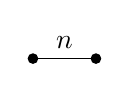
\begin{tikzpicture}[scale=1]
\node at (0.4,0) [above]{$n$};
\draw (0,0)--(0.8,0);
\filldraw
(0,0) circle (.06)
(0.8,0) circle (.06);
\end{tikzpicture}$ when $n\geq 3$, and by $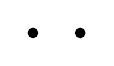
\begin{tikzpicture}[scale=1]
\filldraw
(0,0) circle (.06)
(0.6,0) circle (.06);
\end{tikzpicture}$ when $n=2$.
\end{example}
\begin{example}\label{Coxeter group A_n graph}
The path
\[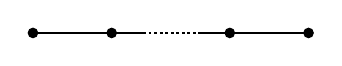
\begin{tikzpicture}[scale=1]
\draw (0,0)--(1,0)--(1.4,0);
\draw[dash pattern=on 1pt off 1pt] (1.4,0)--(2.1,0);
\draw (2.1,0)--(2.5,0)--(3.5,0);
\filldraw
(0,0) circle (.06)
(1,0) circle (.06)
(2.5,0) circle (.06)
(3.5,0) circle (.06);
\end{tikzpicture}\]
is the Coxeter graph of the symmetric group $\mathfrak{S}_n$ with respect to the generating system of adjacent transpositions $s_i=(i,i+1)$, $1\leq i\leq n-1$ (We will see this later). An understanding of this particular example is very valuable, both because of the importance of the symmetric group as such and its role as the most accessible nontrivial example of a Coxeter group. We will frequently return to $\mathfrak{S}_n$ in order to concretely illustrate various general concepts and constructions.
\end{example}
\begin{example}\label{Coxeter group B_n graph}
The graph
\[
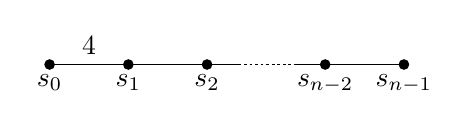
\begin{tikzpicture}[scale=1]
\node at (-0.5,0) [above]{$4$};
\node at (-1,0) [below]{$s_0$};
\node at (0,0) [below]{$s_1$};
\node at (1,0) [below]{$s_2$};
\node at (2.5,0) [below]{$s_{n-2}$};
\node at (3.5,0) [below]{$s_{n-1}$};
\draw (-1,0)--(0,0)--(1,0)--(1.4,0);
\draw[dash pattern=on 1pt off 1pt] (1.4,0)--(2.1,0);
\draw (2.1,0)--(2.5,0)--(3.5,0);
\filldraw
(-1,0) circle (.06)
(0,0) circle (.06)
(1,0) circle (.06)
(2.5,0) circle (.06)
(3.5,0) circle (.06);
\end{tikzpicture}\]
is the Coxeter graph of the group $\mathfrak{S}_n^B$ of all signed permutations of the set $[n]=\{1,2,\dots,n\}$. It can be thought of in terms of the following combinatorial model. Suppose that we have a deck of $n$ cards, such that the $j$-th card has "$+j$" written on one side and "$-j$" on the other. The elements of $\mathfrak{S}_n^B$ can then be identified with the possible rearrangements of stacks of cards; that is, a group element is a permutation of $[n]=\{1,2,\dots,n\}$ (the order of the cards in the stack) together with the sign information $[n]\mapsto\{+,-\}$ (telling which side of each card is up). The Coxeter generators $s_i$ ($1\leq i\leq n-1$) interchange the card in position $i$ with that in position $i+1$ in the stack (preserving orientation), and $s_0$ flips the first card (the top card).\par
The group $\mathfrak{S}_n^B$ has a subgroup, denoted $\mathfrak{S}_n^D$, with Coxeter graph
\[
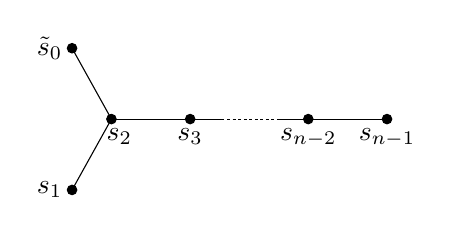
\begin{tikzpicture}[scale=1]
\node at (-0.5,0.9) [left]{$\tilde{s}_0$};
\node at (-0.5,-0.9) [left]{$s_1$};
\node at (0.1,0) [below]{$s_2$};
\node at (1,0) [below]{$s_3$};
\node at (2.5,0) [below]{$s_{n-2}$};
\node at (3.5,0) [below]{$s_{n-1}$};
\draw (-0.5,0.9)--(0,0);
\draw (-0.5,-0.9)--(0,0);
\draw (0,0)--(1,0)--(1.4,0);
\draw[dash pattern=on 1pt off 1pt] (1.4,0)--(2.1,0);
\draw (2.1,0)--(2.5,0)--(3.5,0);
\filldraw
(-0.5,0.9) circle (.06)
(-0.5,-0.9) circle (.06)
(0,0) circle (.06)
(1,0) circle (.06)
(2.5,0) circle (.06)
(3.5,0) circle (.06);
\end{tikzpicture}\]
where $\tilde{s}_0=s_0s_{1}s_0$. In terms of the card model this group consists of the stacks with an even number of turned-over cards (i.e., with minus side up). The generators $s_i$ ($1\leq i\leq n-1$) are adjacent interchanges as before, and $\tilde{s}_0$ flips cards first and the second cards together (as a package).
\end{example}
\begin{example}\label{Coxeter group D_n graph}
The circuit
\[
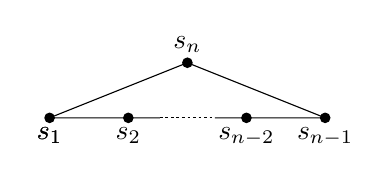
\begin{tikzpicture}[scale=1]
\node at (1.75,0.7) [above]{$s_n$};
\node at (0,0) [below]{$s_1$};
\node at (0,0) [below]{$s_1$};
\node at (1,0) [below]{$s_2$};
\node at (2.5,0) [below]{$s_{n-2}$};
\node at (3.5,0) [below]{$s_{n-1}$};
\draw (1.75,0.7)--(0,0)--(1,0)--(1.4,0);
\draw[dash pattern=on 1pt off 1pt] (1.4,0)--(2.1,0);
\draw (2.1,0)--(2.5,0)--(3.5,0)--(1.75,0.7);
\filldraw
(1.75,0.7) circle (.06)
(0,0) circle (.06)
(1,0) circle (.06)
(2.5,0) circle (.06)
(3.5,0) circle (.06);
\end{tikzpicture}\]
is the Coxeter graph of the group $\widetilde{\mathfrak{S}}_n$ of \textbf{affine permutations} of the integers. This is the group of all permutations $\sigma$ of the set $\Z$ such that
\[\sigma(j+n)=\sigma(j)+n\quad\text{for $j\in\Z$}\]
and
\[\sum_{i=1}^{n}\sigma(i)=\binom{n+1}{2}\]
with composition as group operation. The Coxeter generators are the periodic adjacent transpositions $\tilde{s}_i=\prod_{j\in\Z}(i+jn,i+1+jn)$ for $i=1,\dots,n$.
\end{example}
\begin{example}
The one-way infinite path
\[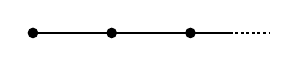
\begin{tikzpicture}[scale=1]
\draw (0,0)--(1,0)--(2,0)--(2.5,0);
\draw[dash pattern=on 1pt off 1pt] (2.5,0)--(3,0);
\filldraw
(0,0) circle (.06)
(1,0) circle (.06)
(2,0) circle (.06);
\end{tikzpicture}\]
is the Coxeter graph of the group of permutations with finite support of the positive integers (i.e., permutations that leave all but a finite subset fixed). The generators are the adjacent transpositions $s_i=(i,i+1)$ with $i\geq 1$.
\end{example}
A Coxeter system $(W,S)$ is said to be \textbf{irreducible} if the underlying graph of its Coxeter graph is connected and non-empty. Equivalently, $S$ is non-empty and there exists no partition of $S$ into two distinct subsets $S_1$ and $S_2$ of $S$ such that every element of $S_1$ commutes with every element of $S_2$. More generally, let $(\Gamma_i)_{i\in I}$ be the family of connected components of $\Gamma$ and let $S_i$ be the set of vertices of $\Gamma_i$. Let $W_i=W_{S_i}$ be the subgroup of W generated by $S_i$. Then the $(W_i,S_i)$ are irreducible Coxeter systems (\cref{Coxeter system W_X subgroup operation prop}) called the irreducible components of $(W,S)$. Moreover, the group $W$ is the restricted direct product\footnote{A group $G$ is the restricted direct product of a family $(G_i)_{i\in I}$ of subgroups if, for any finite subset $J$ of $I$, the subgroup $G_J$ of $G$ generated by the $G_i$ for $i\in J$ is the direct product of the $G_i$ for $i\in J$ and if $G$ is the union of the $G_J$. Equivalently, every element of $G_i$ commutes with every element of $G_j$ for $i\neq j$ and every element of $G$ can be written uniquely as a product $\prod_{i\in I}g_i$ with $g_i\in G_i$ and $g_i=1$ for all but finitely many indices $i$.}. Indeed, this follows from the following more general proposition:
\begin{proposition}\label{Coxeter system restricted product if}
Let $(S_i)_{i\in I}$ be a partition of $S$ such that every element of $S_i$ commutes with every element of $S_j$ if $i\neq j$. For all $i\in I$, let $W_i$ be the subgroup generated by $S_i$. Then $W$ is the restricted direct product of the family $(W_i)_{i\in I}$.
\end{proposition}
\begin{proof}
It is clear that for all $i\in I$ the subgroup $\tilde{W}_i$ generated by the union of the $W_j$ for $j\neq i$ is also generated by $\tilde{S}_i=\bigcup_{j\neq i}S_i$. Thus $W_i\cap\widetilde{W}_i=W_\emp=1$. Since $W$ is generated by the union of the $W_i$, this proves the proposition.
\end{proof}
\subsection{Reduced decompositions for a Coxeter system}\label{Coxeter system reduced decomp paragraph}
Suppose that $(W,S)$ is a Coxeter system. Let $T$ be the set of conjugates in $W$ of elements of $S$. The elements of $T$ (i.e., the elements conjugate to some Coxeter generator) are called \textbf{reflections}. The definition shows that $S\sub T$ and that $t^2=1$ for $t\in T$. The elements of S are sometimes called \textbf{simple reflections}.\par
For any finite sequence $\bm{s}=(s_1,\dots,s_p)$ of elements of $S$, let $w_i=s_1\cdots s_i$ and denote by $\widehat{T}(\bm{s})$ the sequence $(t_1,\dots,t_p)$ of elements of $T$ defined by
\[t_j=(s_1\cdots s_{j-1})s_j(s_1\cdots s_{j-1})^{-1}=w_js_jw_j^{-1}\quad\text{where $w_j=s_1\cdots s_j$ for $1\leq j\leq p$}.\]
Note that we have the following formulas for the sequence $\widehat{T}(\bm{s})$:
\begin{align}\label{Coxeter system t-sequence prop}
t_jw=s_1\cdots\hat{s}_j\cdots s_p,\quad s_1\cdots s_p=t_pt_{p-1}\cdots t_1.
\end{align}
For any element $t\in T$, denote by $n(\bm{s},t)$ the number of integers $j$ such that $t_j=t$.
\begin{proposition}\label{Coxeter system rep on T times pm 1}
Let $(W,S)$ be a Coxeter system and $T$ be the set of conjugates in $W$ of elements of $S$.
\begin{itemize}
\item[(a)] Let $w\in W$ and $t\in T$. Then the number $(-1)^{n(\bm{s},t)}$ has the same value $\eta(w,t)$ for all sequences $\bm{s}=(s_1,\dots,s_p)$ of elements of $S$ such that $w=s_1\dots s_p$.
\item[(b)] For $w\in W$, let $\pi_w$ be the map from $T\times\{\pm 1\}$ to itself defined by
\begin{align}\label{Coxeter system rep on T times pm 1-1}
\pi_w(t,\eps)=(wtw^{-1},\eps\cdot\eta(w^{-1},t)). 
\end{align}
Then the map $w\mapsto \pi_w$ is a homomorphism from $W$ to $\mathfrak{S}_{T\times\{\pm 1\}}$. 
\end{itemize}
\end{proposition}
\begin{proof}
For $s\in S$, define a map $\pi_s$ from $T\times\{\pm 1\}$ to itself by
\begin{align}\label{Coxeter system rep on T times pm 1-2}
\pi_s(t,\eps)=(sts^{-1},\eps\cdot(-1)^{\delta_{st}})
\end{align}
where $(t,\eps)\in T\times\{\pm 1\}$. It is immediate that $\pi_s^2=1$, which shows that $\pi_s$ is a permutation of $T\times\{\pm 1\}$. Let $\bm{s}=(s_1,\dots,s_p)$ be a sequence of elements of $S$. Put $w=s_p\cdots s_1$ and $\pi_{\bm{s}}=\pi_{s_p}\cdots \pi_{s_1}$. We shall show, by induction on $p$, that
\begin{align}\label{Coxeter system rep on T times pm 1-3}
\pi_{\bm{s}}(t,\eps)=(wtw^{-1},\eps\cdot(-1)^{n(\bm{s},t)}).
\end{align}
This is clear for $p=0$. If $p>1$, put $\tilde{\bm{s}}=(s_1,\dots,s_{p-1})$ and $\tilde{w}=s_{p-1}\cdots s_1$. Using the induction hypothesis, we obtain
\begin{align*}
\pi_{\bm{s}}(t,\eps)=\pi_{s_q}(\tilde{w}t\tilde{w}^{-1},\eps\cdot(-1)^{n(\tilde{\bm{s}},t)})=(wtw^{-1},\eps\cdot(-1)^{n(\tilde{\bm{s}},t)+\delta_{s_p,\tilde{w}t\tilde{w}^{-1}}}).
\end{align*}
But $\widehat{T}(\bm{s})=(\widehat{T}(\tilde{\bm{s}}),\tilde{w}^{-1}s_p\tilde{w})$ and $n(\bm{s},t)=n(\tilde{\bm{s}},t)+\delta_{s_p,\tilde{w}t\tilde{w}^{-1}}$, proving formula $(\ref{Coxeter system rep on T times pm 1-3})$.\par
Now let $s,\tilde{s}\in S$ be such that $r=s\tilde{s}$ has finite order $n$. Let $\bm{s}=(s_1,\dots,s_{2n})$ be the sequence of elements of $S$ defined by $s_j=s$ for $j$ odd and $s_j=\tilde{s}$ for $j$ even. Then $s_{2n}\cdots s_1=r^{-n}=1$ and by definition we have
\[t_j=r^{j-1}s\for 1\leq j\leq 2n.\]
Since $r$ is of order $n$, the elements $t_1,\dots,t_n$ are distinct and $t_{j+n}=t$, for $1\leq j\leq n$. For all $t\in T$, the integer $n(\bm{s},t)$ is thus equal to $0$ or $2$ and $(\ref{Coxeter system rep on T times pm 1-3})$ shows that $\pi_{\bm{s}}=1$. In other words, $(\pi_{s}\pi_{\tilde{s}})^n=1$. Thus, by the definition of Coxeter systems, there exists a homomorphism $w\mapsto \pi_w$ from $W$ to $\mathfrak{S}_{T\times\{\pm 1\}}$ such that $\pi_s$ is given by the right-hand side of $(\ref{Coxeter system rep on T times pm 1-3})$. Then by the homomorphism property, we have $\pi_w=\pi_{\bm{s}}$ for every sequence $\bm{s}=(s_1,\dots,s_p)$ such that $w=s_p\cdots s_1$ and from $(\ref{Coxeter system rep on T times pm 1-3})$ we see $(-1)^{n(\bm{s},t)}$ shares a common value $\eta(w,t)$ for such a sequence $\bm{s}$. This proves the proposition.
\end{proof}
We now come to the so-called "exchange property," which is a fundamental combinatorial property of a Coxeter group. In its basic version, the condition $t\in T$ in the statement below is weakened to $t\in S$, hence the adjective "strong" for the version given here.
\begin{proposition}[\textbf{Strong Exchange Property}]\label{Coxeter system exchange property}
Let $(W,S)$ be a Coxeter system, $w\in W$ and $t\in T$. Let $\eta(w,t)$ be the number defined in \cref{Coxeter system rep on T times pm 1}. Then the following conditions are equivalent.
\begin{itemize}
\item[(\rmnum{1})] $\ell(tw)<\ell(w)$;
\item[(\rmnum{2})] $\eta(w,t)=-1$.
\end{itemize}
If these conditions are satisfied, then for any sequence $\bm{s}=(s_1,\dots,s_p)$ of elements of $S$ with $w=s_1\cdots s_p$ there exists an integer $j$ such that
\[t_j=s_1\cdots s_{j-1}s_j(s_1\cdots s_{j-1})^{-1}=t.\]
\end{proposition}
\begin{proof}
First, assume that $\eta(w,t)=-1$, and choose a reduced decomposition $\bm{s}=(s_1,\dots,s_p)$ of $w$. Then by \cref{Coxeter system rep on T times pm 1} we have $\eta(w,t)=(-1)^{n(\bm{s},t)}$, whence $n(\bm{s},t)$ is odd. In particular, since $n(\bm{s},t)\neq 0$, we have $t=t_j$ for some $j$, so
\[\ell(tw)=\ell(s_1\cdots\hat{s}_j\cdots s_p)\leq p-1<p=\ell(w).\]
Conversely, if $\eta(w,t)=1$, then using $(\ref{Coxeter system rep on T times pm 1-1})$, we get
\begin{align*}
\pi_{(tw)^{-1}}(t,\eps)&=\pi_{w^{-1}}\pi_t(t,\eps)=\pi_{w^{-1}}(t,-\eps)\\
&=(w^{-1}tw,-\eps\cdot\eta(w,t))=(w^{-1}tw,-\eps).
\end{align*}
This means that $\eta(tw,t)=-1$, which by the implication (\rmnum{2})$\Rightarrow$(\rmnum{1}) already proved shows that $\ell(ttw)<\ell(tw)$, that is, $\ell(w)<\ell(tw)$.\par
Fianlly, assume the given conditions, and choose a sequence $\bm{s}=(s_1,\dots,s_p)$ of elements of $S$ with $w=s_1\cdots s_p$. Then, since $\eta(w,t)=(-1)^{n(\bm{s},t)}$, we deduce that $n(\bm{s},t)$ is odd, and hence that $t=t_j$ for some $j$. Therefore, $tw=s_1\cdots\hat{s}_j\cdots s_p$.
\end{proof}
\begin{corollary}\label{Coxeter system l(tw) leq l(w) iff commutes}
Let $(W,S)$ be a Coxeter system, $w\in W$ and $t\in T$. If $\bm{s}=(s_1,\dots,s_p)$ is a reduced sequence for $w$, then the follwing are equivalent:
\begin{itemize}
\item[(\rmnum{1})] $\ell(tw)<\ell(w)$;
\item[(\rmnum{2})] $tw=s_1\cdots\hat{s}_j\cdots s_p$ for some $j$;
\item[(\rmnum{3})] $t=(s_1\cdots s_{j-1})s_j(s_1\cdots s_{j-1})^{-1}$ for some $j$.
\end{itemize}
\end{corollary}
\begin{proof}
The equivalence (\rmnum{2})$\Leftrightarrow$(\rmnum{3}) is easy to see (and does not require the hypothesis that $\bm{s}$ is reduced). \cref{Coxeter system exchange property} shows that (\rmnum{1})$\Rightarrow$(\rmnum{2}), and the converse is obvious.
\end{proof}
We now consider the following sets:
\begin{align}\label{Coxeter system associated reflection def}
T_L(w)=\{t\in T:\ell(tw)<\ell(w)\},\quad T_R(w)=\{t\in T:\ell(wt)<\ell(w)\}.
\end{align}
In this notation "$L$" and "$R$" are mnemonic for "left" and "right." The set $T_L(w)$ is called the set of \textbf{left associated reflections} to $w$, and similarly for $T_R(w)$. Corollary~\ref{Coxeter system l(tw) leq l(w) iff commutes} gives some useful characterizations of the set $T_L(w)$, and we have a similar description for $T_R(w)$ by applying these to $w^{-1}$, since clearly $T_R(w)=T_L(w^{-1})$.
\begin{proposition}\label{Coxeter system reduced iff t-sequence distinct}
Let $(W,S)$ be a Coxeter system, $w\in W$, $\bm{s}=(s_1,\dots,s_p)$ be a sequence such that $w=s_1\cdots s_p$, and $\widehat{T}(\bm{s})=(t_1,\dots,t_p)$. Then the sequence $\bm{s}$ is a reduced decomposition of $w$ if and only if the $t_j$ are distinct, and in that case $T_L(w)=\{t_1,\dots,t_p\}$ and $|T_L(w)|=\ell(w)$.
\end{proposition}
\begin{proof}
If $t\in T_L(w)$, then $n(\bm{s},t)=-1$ so $t$ equals to at least one of the $t_j$'s, hence $T_w\sub\{t_1,\dots,t_p\}$, whence $|T_w|\leq\ell(w)$ since $\bm{s}$ is arbitrary. If the $t_j$ are distinct, then $n(\bm{s},t)$ is equal to $1$ or $0$ according to whether $t$ does or does not belong to $\{t_1,\dots,t_p\}$. It follows that $T_w=\{t_1,\dots,t_p\}$ and that $p=|T_w|\leq\ell(w)$, which implies that $\bm{s}$ is reduced.\par
Suppose finally that $t_i=t_j$ with $i<j$. This gives $s_i=us_ju^{-1}$ with $u=s_{i+1}\cdots s_{j-1}$, hence
\[w=w_{i-1}s_ius_js_{j+1}\cdots s_p=w_{i-1}us_js_js_{j+1}\cdots s_p=s_1\cdots\hat{s}_i\cdots\hat{s}_j\cdots s_p.\]
This shows that $\bm{s}$ is not a reduced decomposition of $w$.
\end{proof}
\begin{corollary}\label{Coxeter system T_L(w) char by product}
Let $(W,S)$ be a Coxeter system and $w\in W$. Then the set $T_L(w)$ consists of elements in $T$ of the form $w_2sw_2^{-1}$ corresponding to the triples $(w_1,w_2,s)\in W\times W\times S$ such that $w=w_2sw_1$ and $\ell(w_1)+\ell(w_2)+1=\ell(w)$.
\end{corollary}
\begin{proof}
By \cref{Coxeter system reduced iff t-sequence distinct}, if $\bm{s}=(s_1,\dots,s_p)$ is a reduced decomposition of $w$ and $\widehat{T}(\bm{s})=(t_1,\dots,t_p)$, then $T_L(w)=\{t_1,\dots,t_p\}$. Now each element $t_j$ can be written as
\[t_j=w_2s_jw_2^{-1}\quad\text{where $w_2=s_1\cdots s_{j-1}$}\]
and therefore
\[w=w_2s_jw_1\quad\text{where $w_1=s_{j+1}\cdots s_p$}.\]
Moreover, since $\bm{s}$ is reduced, we have $\ell(w_2)=j-1$ and $\ell(w_1)=p-j$, whence $\ell(w)=\ell(w_1)+\ell(w_2)+1$.\par
Conversely, if $t=w_2sw_s^{-1}$ where $(w_1,w_2,s)$ is a triple such that $w=w_2sw_1$ and $\ell(w_1)+\ell(w_2)+1=\ell(w)$, then
\[\ell(tw)=\ell(w_2sw_2^{-1}w)=\ell(w_2w_1)\leq\ell(w_2)+\ell(w_1)=\ell(w)-1<\ell(w)\]
whence $t\in T_L(w)$. This completes the proof. 
\end{proof}
We will quite often need to refer to the associated simple reflections, for
which we introduce the following special notation and terminology:
\[D_L(w)=T_L(w)\cap S=\{s\in S:\ell(sw)<\ell(w)\},\quad D_R(w)=\{s\in S:\ell(ws)<\ell(w)\}.\]
The set $D_R(w)$ is called the \textbf{right descent set}, and similarly for $D_L(w)$. Their elements are called \textbf{right} (resp. \textbf{left}) \textbf{descents}. The reason for this terminology will become clear when we specialize to the symmetric groups. Still, we have $D_R(w)=D_L(w^{-1})$.
\begin{corollary}\label{Coxeter system descent set iff}
Let $(W,S)$ be a Coxeter system. For all $s\in S$ and $w\in W$, the following hold:
\begin{itemize}
\item[(a)] $s\in D_L(w)$ if and only if some reduced expression for $w$ begins with the letter $s$.
\item[(b)] $s\in D_R(w)$ if and only if some reduced expression for w ends with the letter $s$.
\end{itemize}
\end{corollary}
\begin{proof}
One direction is clear, and the other direction follows easily from Corollary~\ref{Coxeter system l(tw) leq l(w) iff commutes}.
\end{proof}
\begin{proposition}[\textbf{Deletion Property}]\label{Coxeter system deletion property}
Let $(W,S)$ be a Coxeter system, $w\in W$, and $\bm{s}=(s_1,\dots,s_p)$ be a sequence such that $w=s_1\cdots s_p$. If $\bm{s}$ is not reduced for $w$, then there exists indices $i<j$ such that $w=s_1\cdots\hat{s}_i\cdots\hat{s}_j\cdots s_p$.
\end{proposition}
\begin{proof}
This is contained in the proof of \cref{Coxeter system reduced iff t-sequence distinct}.
\end{proof}
\begin{corollary}
Let $(W,S)$ be a Coxeter system. Then any expression $w=s_1\cdots s_p$ contains a reduced expression for $w$ as a subword, obtainable by deleting an even number of letters.
\end{corollary}
\begin{proposition}\label{Coxeter group conjugate iff}
Assume that $(W,S)$ is a Coxeter system. Then, two elements $s$ and $\tilde{s}$ of $S$ are conjugate in $W$ if and only if the following condition is satisfied: there exists a finite sequence $(s_1,\dots,s_p)$ of elements of $S$ such that $s_1=s,s_p=\tilde{s}$ and $s_is_{i+1}$ is of finite odd order for $1\leq i<p$.
\end{proposition}
\begin{proof}
Let $s$ and $\tilde{s}$ in $S$ be such that $r=s\tilde{s}$ is of finite order $2n+1$. Then we have $srs=r^{-1}$, hence
\[r^nsr^{-n}=r^nr^ns=r^{-1}s=\tilde{s}ss=\tilde{s}\]
and $\tilde{s}$ is conjugate to $s$.\par
For a fixed $s$ in $S$, let $C_s$ be the set of $\tilde{s}\in S$ satisfying the prescribed condition. Then by the above argument, the elements $s_i$ and $s_{i+1}$ are conjugate for $1\leq i<p$ by the above, hence every element $\tilde{s}$ of $C_s$ is conjugate to $s$. Now define a map $f:S\to\{\pm 1\}$ which equals to $1$ on $C_s$ and to $-1$ on $S\setminus C_s$. Let $s_1$ and $s_2$ in $S$ be such that $s_1s_2$ is of finite order $n$. Then $f(s_1)f(s_2)=1$ if $s_1$ and $s_2$ are both in $C_s$ or both in $S\setminus C_s$. In the other case, $f(s_1)f(s_2)=-1$, but $n$ is even. Thus $(f(s_1)f(s_2))^n=1$ in all cases. Since $(W,S)$ is a Coxeter system, there exists a extension of $f$ on $W$, which we still denote by $f$. Let $\tilde{s}\in S$ be a conjugate of $s$. Since $s$ belongs to the kernel of $f$, so does $\tilde{s}$, hence $f(\tilde{s})=1$ and finally $\tilde{s}\in C_s$.
\end{proof}
\subsection{Characterization of Coxeter systems}
The statement that the Exchange Property is fundamental in the combinatorial theory of Coxeter groups can be made very precise: It characterizes such groups! This is often a convenient way to prove that a given group is a Coxeter group.\par
Throughout this paragraph we assume that $W$ is an arbitrary group and that $S\sub W$ is a generating subset such that $s^2=1$ for all $s\in S$. For such a pair, we define the "Exchange Property" and "Deletion Property" as follows.
\begin{enumerate}[leftmargin=20pt]
\item[(E)] Let $w\in W$ and $s\in S$ be such that $\ell(sw)\leq\ell(w)$. Then for any reduced decomposition $(s_1,\dots,s_p)$ of $w$, there exists an integer $j$ such that $s=s_1\cdots s_{j-1}s_j(s_1\cdots s_{j-1})^{-1}$.
\item[(D)] Let $w\in W$ and $s\in S$. If $(s_1,\dots,s_p)$ is not a reduced decomposition of $w$, then there exists integers $i<j$ such that $w=s_1\cdots\hat{s}_i\cdots\hat{s}_j\cdots s_p$.
\end{enumerate}
By \cref{Coxeter system exchange property}, we see $(W,S)$ satisfies this condition if it is a Coxeter system.
\begin{proposition}\label{E system decomposition of sw}
Let $(W,S)$ be a system satisfying (E). Let $s\in S$, $w\in W$ and $\bm{s}=(s_1,\dots,s_p)$ be a reduced decomposition of $w$. Then one of the following must hold:
\begin{itemize}
\item[(\rmnum{1})] $\ell(sw)=\ell(w)+1$ and $(s,s_1,\dots,s_p)$ is a reduced decomposition of $sw$.
\item[(\rmnum{2})] $\ell(sw)=\ell(w)-1$ and there exists an integer $j$ such that $(s_1,\dots,\hat{s}_j,\dots,s_p)$ is a reduced decomposition of $sw$ and $(s,s_1,\dots,\hat{s}_j,\dots,s_p)$ is a reduced decomposition of $w$.
\end{itemize}
\end{proposition}
\begin{proof}
Put $\tilde{w}=sw$, then we have $\ell(\tilde{w})=\ell(w)\pm 1$. We distinguish two cases. If $\ell(\tilde{w})>\ell(w)$ then $\ell(\tilde{w})=p+1$ and $\tilde{w}=ss_1\cdots s_p$, so $(s,s_1,\dots,s_p)$ is a reduced decomposition of $\tilde{w}$. If $\ell(\tilde{w})\leq\ell(w)$, then by (E), there exists an integer $j$ such that $s=t_j$. Then $\tilde{w}=s_1\cdots\hat{s}_j\cdots s_p$ and hence $w=ss_1\cdots\hat{s}_j\cdots s_p$. It then follows that $\ell(\tilde{w})=p-1$ and that $(s_1,\dots,\hat{s}_j,\dots,s_p)$ is a reduced decomposition of $\tilde{w}$.
\end{proof}
\begin{lemma}\label{E system spacial map constant}
Let $(W,S)$ be a system satisfying (E). Let $w\in W$ have length $p\geq 1$, let $D$ be the set of reduced decompositions of $w$ and let $f:D\to E$ be a map from $D$ to a set $E$. Assume that $f(s)=f(\tilde{s})$ if the elements $\bm{s}=(s_1,\dots,s_p)$, $\tilde{\bm{s}}=(\tilde{s}_1,\dots,\tilde{s}_p)$ of $D$ satisfy one of the following hypotheses:
\begin{itemize}
\item[(a)] $s_1=\tilde{s}_1$ or $s_p=\tilde{s}_p$. 
\item[(b)] There exist $s$ and $\tilde{s}$ in $S$ such that $s_i=\tilde{s}_j=s$ and $s_j=\tilde{s}_i=\tilde{s}$ for every $i$ odd and $j$ even.
\end{itemize}
Then $f$ is constant.
\end{lemma}
\begin{proof}
Let $\bm{s},\tilde{\bm{s}}\in D$ and put $\bm{t}=(\tilde{s}_1,s_1,\dots,s_{p-1})$. We are going to show that if $f(\bm{s})\neq f(\tilde{\bm{s}})$ then $\bm{t}\in D$ and $f(\bm{t})\neq f(\bm{s})$. Indeed, $w=\tilde{s}_1\cdots\tilde{s}_p$; and hence $\tilde{s}_1w=\tilde{s}_2\cdots\tilde{s}_p$ is of length $<p$. By \cref{E system decomposition of sw}, there exists an integer $j$ such that the sequence $\bm{u}=(\tilde{s}_1,s_1,\dots,\hat{s}_j,\dots,s_p)$ belongs to $D$. We have $f(\bm{u})=f(\tilde{\bm{s}})$ by condition (a); if $j\neq p$ we would have $f(\bm{s})=f(\bm{u})$ for the same reason, and hence $f(\bm{s})=f(\tilde{\bm{s}})$ contrary to our hypothesis. Thus $j=p$ and hence $\bm{t}=\bm{u}\in D$ and $f(\bm{t})=f(\tilde{\bm{s}})\neq f(\bm{s})$.\par
For any integer $j$ with $0\leq j\leq p+1$, define a sequence $\bm{s}_j$ of $p$ elements of $S$ as follows:
\begin{align*}
\bm{s}_0&=(\tilde{s}_1,\dots,\tilde{s}_p)\\
\bm{s}_{p-k+1}&=(s_1,\tilde{s}_1,\dots,s_1,\tilde{s}_1,s_1,\dots,s_k)\quad \text{for $p-k$ even and $0\leq k\leq p$}\\
\bm{s}_{p-k+1}&=(\tilde{s}_1,s_1,\dots,s_1,\tilde{s}_1,s_1,\dots,s_k)\quad \text{for $p-k$ odd and $0\leq k\leq p$}.
\end{align*}
Denote by ($H_j$) the assertion "$\bm{s}_j,\bm{s}_{j+1}\in D$ and $f(\bm{s}_j)\neq f(\bm{s}_{j+1})$." By the preceding argument, ($H_j$) implies ($H_{j+1}$) for $0\leq j<p$, and ($H_p$) is not satisfied by condition (b). Hence, ($H_0$) is not satisfied. Since $\bm{s}_0=\tilde{\bm{s}}$ and $\bm{s}_1=\bm{s}$, it follows that $f(\bm{s})=f(\tilde{\bm{s}})$.
\end{proof}
\begin{proposition}\label{E system symmetric map on S extension to W}
Let $(W,S)$ be a system satisfying (E). Let $M$ be a monoid (with unit element $1$) and $f:S\to M$ a map. For $s,\tilde{s}\in S$, let $m(s,\tilde{s})$ be the order of $s\tilde{s}$ and put
\[\alpha(s,\tilde{s})=\begin{cases}
(f(s)f(\tilde{s}))^k&\text{if $m(s,\tilde{s})=2k$, $k$ finite}\\
(f(s)f(\tilde{s}))^kf(s)&\text{if $m(s,\tilde{s})=2k+1$, $k$ finite}\\
1&\text{if $m(s,\tilde{s})=\infty$}.
\end{cases}\]
If $\alpha(s,\tilde{s})=\alpha(\tilde{s},s)$ whenever $s\neq\tilde{s}$ are in $S$, then there exists a map $f:W\to M$ such that
\[g(w)=f(s_1)\cdots f(s_p)\]
for all $w\in W$ and any reduced decomposition $(s_1,\dots,\tilde{s}_p)$ of $w$.
\end{proposition}
\begin{proof}
For any $w\in W$, let $D_w$ be the set of reduced decompositions of $w$ and $f_w:D_w\to M$ the map defined by
\[f_w(s_1,\dots,s_p)=f(s_1)\cdots f(s_p).\]
We are going to prove by induction on the length of $w$ that $f_w$ is constant, which will establish the proposition. The cases $\ell(w)=0,1$ being trivial, we assume that $p\geq 2$ and that our assertion is proved for the elements to with $\ell(w)<p$. Let $w$ be of length $p$ and $\bm{s},\tilde{\bm{s}}\in D_w$; by \cref{E system spacial map constant} it suffices to prove that $f_w(\bm{s})=f_w(\tilde{\bm{s}})$ in cases (a) and (b) of that Lemma.\par
In case (a), the formula
\[f_w(s_1,\dots,s_p)=f(s_1)f_{w_2}(s_2,\dots,s_p)=f_{w_1}(s_1,\dots,s_{p-1})f(s_p)\]
for $w_1=s_1\dots s_{p-1}$ and $w_2=s_2\dots s_p$ and the induction hypothesis show that $f_w(\bm{s})=f_w(\bm{s})$ if $s_1=\tilde{s}_1$ or $s_p=\tilde{s}_p$.\par
Suppose that there exist two elements $s$ and $\tilde{s}$ of $S$ such that $s_i=\tilde{s}_j=s$ and $s_j=\tilde{s}_i=\tilde{s}$ for every $i$ odd and $j$ even. It suffices to treat the case $s\neq \tilde{s}$, since otherwise $\bm{s}=\tilde{\bm{s}}$. In this case, the sequences $\bm{s}$ and $\tilde{\bm{s}}$ are then two distinct reduced decompositions of $w$ in the dihedral group generated by $s$ and $\tilde{s}$, whence the order $n$ of $s\tilde{s}$ is finite. In the notation of $(\ref{Dihedral group sequence})$, we have $\bm{s}=\bm{s}_n$ and $\tilde{\bm{s}}=\tilde{\bm{s}}_n$. Consequently, $f_w(\bm{s})=\alpha(\bm{s},\tilde{\bm{s}})$ and $f_w(\tilde{\bm{s}})=\alpha(\tilde{\bm{s}},\bm{s})$, hence $f_w(\bm{s})=f_w(\tilde{\bm{s}})$.
\end{proof}
\begin{theorem}\label{Coxeter system iff exchange iff deletion}
For a system $(W,S)$, the following conditions are equivalent.
\begin{itemize}
\item[(\rmnum{1})] $(W,S)$ is a Coxeter system;
\item[(\rmnum{2})] $(W,S)$ has the Exchange Property;
\item[(\rmnum{3})] $(W,S)$ has the Deletion Property.
\end{itemize}
\end{theorem}
\begin{proof}
Denote by (E) the exchange Property, and by (D) the Deletion Property.
\cref{Coxeter system exchange property} shows that any Coxeter system satisfies (E), and \cref{Coxeter system deletion property} shows that any coxeter system satisfies (D). Conversely, suppose that (E) is satisfied. Let $G$ be a group and $f:S\to G$ a map such that $(f(s)f(\tilde{s}))^n=1$ whenever $s$ and $\tilde{s}$ belong to $S$ and $s\tilde{s}$ is of finite order $n$. Then by $f$ satisfies the condition in \cref{E system symmetric map on S extension to W}, so there exists a map $g:W\to G$ such that
\[g(w)=f(w_1)\cdots f(w_p)\]
whenever $w=s_1\cdots s_p$ is of length $p$. To prove that $(W,S)$ is a Coxeter system, it suffices to prove that $g$ is a homomorphism, which is a consequence of the formula
\[g(sw)=f(s)g(w)\for s\in S,w\in W.\]
since $S$ generates $W$. This follows by applying \cref{E system decomposition of sw}.\par
Fianlly, we show that (\rmnum{3})$\Rightarrow$(\rmnum{1}). Suppose that $\ell(sw)<\ell(w)=p$. Then, by the Deletion Property, two letters can be deleted from $ss_1\cdots s_p$, giving a new expression for $sw$. If $s$ is not one of these letters, then $ss_1\cdots s_p=ss_1\cdots\hat{s}_i\cdots\hat{s}_j\cdots s_p$ would give
\[\ell(w)=\ell(s_1\cdots\hat{s}_i\cdots\hat{s}_j\cdots s_p)<p,\]
a contradiction. Hence, $s$ must be one of the deleted letters and we obtain $sw=ss_1\cdots s_p=s_1\cdots\hat{s}_j\cdots s_p$. This completes the proof.
\end{proof}
\begin{remark}
The Exchange Property is stated above in its "left" version, since we are acting with $s$ on the left of $w$. There is, of course, a "right" version (replace $sw$ by $ws$), which is equivalent as a consequence of \cref{Coxeter system iff exchange iff deletion}.
\end{remark}
\subsection{Coxeter system defined by partitions}
\begin{proposition}\label{Coxeter system ABC conditions}
Suppose that $(W,S)$ is a Coxeter system. For any $s\in S$, let $P_s$ be the set of elements $w\in W$ such that $\ell(sw)>\ell(w)$. We have the following properties:
\begin{enumerate}[leftmargin=20pt]
\item[(A)] $\bigcap_{s\in S}P_s=\{1\}$.
\item[(B)] For any $s$ in $S$, the sets $P_s$ and $sP_s$ form a partition of $W$.
\item[(C)] Let $s,\tilde{s}$ be in $S$ and let $w$ be in $W$. If $w\in P_s$ and $w\tilde{s}\notin P_s$ then $s=w\tilde{s}w^{-1}$.   
\end{enumerate}
\end{proposition}
\begin{proof}
For (A), let $w\neq 1$ be in $W$ and let $(s_1,\dots,s_p)$ be a reduced decomposition of $w$. Then $p\geq 1$ and $(s_2,\dots,s_p)$ is a reduced decomposition of $s_1w$, so $\ell(w)=p$ and $\ell(s_1w)=p-1$. Hence $w\notin P_{s_1}$.\par
To prove (B), let $w\in W$ and $s\in S$. If $\ell(sw)=l(w)+1$ then $w\in P_s$. On the other hand, if $\ell(sw)=\ell(w)-1$, put $\tilde{w}=sw$ so that $w=s\tilde{w}$; then $\ell(\tilde{w})<\ell(s\tilde{w})$ hence $\tilde{w}\in P_s$ and so $w\in sP_s$.\par
Let $s,\tilde{s}\in S$ and $w\in W$ be as in (C); let $p$ be the length of $w$. From $w\in P_s$ it follows that $\ell(sw)=p+1$; and from $w\tilde{s}\notin P_s$ it follows that $\ell(sw\tilde{s})=\ell(w\tilde{s})-1\leq p$. Since $\ell(sw\tilde{s})=\ell(sw)\pm 1$, we have finally that $\ell(w\tilde{s})=p+1$ and $\ell(sw\tilde{s})=p$. Let $(s_1,\dots,s_p)$ be a reduced decomposition of $w$ and $s_{p+1}=\tilde{s}$; then $(s_1,\dots,s_{p+1})$ is a reduced decomposition of the element $w\tilde{s}$ of length $p+1$. Since $\ell(sw\tilde{s})=p$, by the exchange condition there exists an integer $j$ with $1\leq j\leq p+1$ such that
\[s=(s_1\cdots s_{j-1})s_j(s_1\cdots s_{j-1})^{-1}.\]
If $1\leq j\leq p$, we would have $sw=s_1\cdots\hat{s}_j\cdots s_p$, contradicting the formula $\ell(sw)=p+1$. Thus $j=p+1$ and we get $s=w\tilde{s}w^{-1}$.
\end{proof}
Conversely, we have the following result:
\begin{proposition}\label{Coxeter system if A'B'C conditions}
Let $(P_s)_{s\in S}$ be a family of subsets of $W$ satisfying (C) and the following conditions:
\begin{enumerate}
\item[(A')] $1\in P_s$ for all $s\in S$.
\item[(B')] The sets $P_s$ and $sP_s$ are disjoint for all $s\in S$.
\end{enumerate}
Then $(W,S)$ is a Coxeter system and $P_s$ consists of the elements $w\in W$ such that $\ell(sw)>\ell(w)$.
\end{proposition}
\begin{proof}
Let $s\in S$ and $w\in W$. If $w\notin P_s$, let $(s_1,\dots,s_p)$ be a reduced decomposition of $w$ and $w_j=s_1\cdots s_j$ for $1\leq i\leq p$; also put $w_0=1$. Since $w_0\in P_s$ by (A') and since $w_p=w$ is not in $P_s$, there exists an integer $j$ with $1\leq j<p$ such that $w_{j-1}\in P_s$ and $w_j=w_{j-1}s_j$ does not belong to $P_s$. By (C), we therefore have
\[ss_1\cdot ss_{j-1}=s_1\cdots s_{j-1}s_j.\]
Which implies that $sw=s_1\cdots\hat{s}_j\cdots s_p$ and $\ell(sw)<\ell(w)$. Note that we have also showed that the exchange condition holds for $(W,S)$, so it is a Coxeter system.\par
On the other hand, assume that $w\in P_s$. Put $\tilde{s}=sw$, so that $\tilde{w}\notin P_s$ by (B'). By the preceding argument, we then have $\ell(s\tilde{w})<\ell(\tilde{w})$, that is $\ell(w)<\ell(sw)$. It then follows that $P_s$ consists of those $w\in W$ such that $\ell(sw)>\ell(w)$.
\end{proof}
\subsection{Subgroups of a Coxeter group}
Let $(W,S)$ is a Coxeter system. For any subset $X$ of $S$, we denote by $W_X$ the subgroup of $W$ generated by $X$.
\begin{proposition}\label{Coxeter system decomposition image set equal}
Let $(W,S)$ be a a Coxeter system and $w$ be in $W$. There exists a subset $S_w$ of $S$ such that $\{s_1,\dots,s_p\}=S_w$ for any reduced decomposition $(s_1,\dots,s_p)$ of $w$.
\end{proposition}
\begin{proof}
Denote by $M$ the monoid consisting of the subsets of $S$ with the composition law $(A,B)\mapsto A\cup B$; the identity element of $M$ is $\emp$. Put $f(s)=\{s\}$ for $s\in S$. We are going to apply \cref{E system symmetric map on S extension to W} to $M$ and $f$. We have $\alpha(s,\tilde{s})=\{s,\tilde{s}\}$ for $s,\tilde{s}$ in $S$ if $m(s,\tilde{s})$ is finite, hence there exists a map $g:w\mapsto S_w$ from $W$ to $M$ such that $g(w)=f(s_1)\cup\cdots\cup(s_p)$. Therefore $S_w=\{s_1,\dots,s_p\}$ for any $w\in W$ and any reduced decomposition $(s_1,\dots,s_p)$ of $w$.
\end{proof}
\begin{example}
Let $n$ be an integer and consider the Coxeter group $D_n$ generated by $\{s,\tilde{s}\}$. Recall that if $n$ is finite then the element $w_n$ in $(\ref{Dihedral group sequence})$ have two reduced decomposition, and we have $S_{w_n}=\{s,\tilde{s}\}$, verifying \cref{Coxeter system decomposition image set equal}.
\end{example}
\begin{corollary}\label{Coxeter system subgroup W_X char}
Let $(W,S)$ is a Coxeter system. For any subset $X$ of $S$, the subgroup $W_X$ of $W$ consists of the elements $w$ of $W$ such that $S_w\sub X$.
\end{corollary}
\begin{proof}
If $w=(s_1,\dots,s_p)$ with $s_1,\dots,s_p$ in $S$, then $w^{-1}=s_p\cdots s_1$, hence $S_w=S_{w^{-1}}$. \cref{E system decomposition of sw} shows that $S_{sw}\sub \{s\}\cup S_w$ for $s\in S$ and $w\in W$, which implies the formula $S_{w\tilde{w}}\sub S_w\cup S_{\tilde{w}}$ by induction on the length of $w$. Therefore, the set $U$ of $w\in W$ such that $S_w\sub X$ is a subgroup of $W$; we have $X\sub U\sub W_X$, hence $U=W_X$.
\end{proof}
\begin{corollary}\label{Coxeter system W_X intersection with S}
Let $(W,S)$ is a Coxeter system. For any subset $X$ of $S$, we have $W_X\cap S=X$.
\end{corollary}
\begin{proof}
This follows from Corollary~\ref{Coxeter system subgroup W_X char} and the formula $S_s=\{s\}$ for $s$ in $S$.
\end{proof}
\begin{corollary}\label{Coexter group W_X length function is restriction}
Let $(W,S)$ is a Coxeter system. For any subset $X$ of $S$ and any $w$ in $W_X$, the length of $w$ with respect to the generating set $X$ of $W_X$ is equal to $\ell_S(w)$.
\end{corollary}
\begin{proof}
Let $(s_1,\dots,s_p)$ be a reduced decomposition of $w$ considered as an element of $W$. We have $w=s_1\dots s_p$ and $s_i\in X$ for $1\leq i\leq p$. Moreover, $w$ cannot be a product of $q<p$ elements of $X\sub S$ by definition of $p=\ell_S(w)$, so $\ell_X(w)=p=\ell_S(w)$.
\end{proof}
\begin{proposition}\label{Coxeter system W_X subgroup operation prop}
Let $(W,S)$ is a Coxeter system.
\begin{itemize}
\item[(a)] For any subset $X$ of $S$, the pair $(W_X,X)$ is a Coxeter system.
\item[(b)] Let $(X_\alpha)_{\alpha\in A}$ be a family of subsets of $S$. If $X=\bigcap_\alpha X_\alpha$, then $W_X=\bigcap_\alpha W_{X_\alpha}$.
\item[(c)] Let $X$ and $Y$ be two subsets of $S$. Then $W_X\sub W_Y$ if and only if $X\sub Y$.
\end{itemize}
\end{proposition}
\begin{proof}
Every element of $X$ is of order $2$ and $X$ generates $W_X$. Let $s\in X$ and $w\in W_X$ with $\ell_X(sw)\leq\ell_X(w)=p$. By Corollary~\ref{Coexter group W_X length function is restriction}, we have $\ell_S(sw)\leq\ell_S(w)=p$. Let $s_1,\dots,s_p$ be elements of $X$ such that $w=s_1\cdots s_p$. Since $(W,S)$ satisfies the exchange condition, there exists an integer $j$ such that $s=(s_1\cdots s_{j-1})s_j(s_1\cdots s_{j-1})^{-1}$. Thus, $(W_X,X)$ satisfies the exchange condition and is therefore a Coxeter system. This proves (a), and assertions (b) and (c) follow immediately from Corollary~\ref{Coxeter system subgroup W_X char}.
\end{proof}
\section{Tits systems}
\subsection{Tits systems and Bruhat decompositions}
Let $G$ be a group and $B$ a subgroup of $G$. The group $B\times B$ acts on $G$ by $(b,\tilde{b})\cdot g=bg\tilde{b}^{-1}$ for $b,\tilde{b}\in B$ and $g\in G$. The orbits of $B\times B$ on $G$ are the sets $BgB$ for $g\in G$, and are called the double cosets of $G$ with respect to $B$. They form a partition of $G$; the corresponding quotient is denoted by $B\backslash G/B$. If $C$ and $\widetilde{C}$ are double cosets, $C\tilde{C}$ is a union of double cosets.
\begin{definition}
A \textbf{Tits system} is a quadruple $(G,B,N,S)$, where $G$ is a group, $B$ and $N$ are two subgroups of $G$ and $S$ is a subset of $N/(B\cap N)$, satisfying the following axioms:
\begin{itemize}
\item[(T1)] The set $B\cup N$ generates $G$ and $B\cap N$ is a normal subgroup of $N$.
\item[(T2)] The set $S$ generates the group $W=N/(B\cap N)$ and consists of elements of order $2$.
\item[(T3)] $sBw\sub BwB\cup BswB$ for $s\in S$ and $w\in W$\footnote{Every element of $W$ is a coset modulo $B\cap N$, and is thus a subset of $G$; hence products such as $BwB$ make sense. More generally, for any subset $A$ of $W$, we denote by $BAB$ the subset $\bigcup_{w\in A}BwB$.}.
\item[(T4)] For all $s\in S$, $sBs\nsubseteq B$.  
\end{itemize}
\end{definition}
\begin{remark}
Let $(G,B,N,S)$ be a Tits system, and let $Z$ be a normal subgroup of $G$ contained in $B$. Let $\tilde{G}=G/Z$, $\tilde{B}=B/Z$, $\tilde{N}=N/(Z\cap N)$, and let $\tilde{S}$ be the image of $S$ in $\tilde{N}/(\tilde{B}\cap\tilde{N})$. Then one sees immediately that $(\tilde{G},\tilde{B},\tilde{N},\tilde{S})$ is a Tits system.
\end{remark}
Throughout this paragraph, let $(G,B,N,S)$ be a Tits system. We set $T=B\cap N$ and $W=N/T$. A double coset means a double coset of $G$ with respect to $B$. For any $w\in W$, we set $C(w)=BwB$; this is a double coset.\par
We first deduce several elementary consequences of the axioms (T1) to (T4). We denote by $w,\tilde{w},\dots$ elements of $W$ and by $s,\tilde{s},\dots$ elements of $S$. The following relations are clear:
\begin{align}\label{Tits system prop-1}
C(1)=B,\quad C(w\tilde{w})\sub C(w)C(\tilde{w}),\quad C(w^{-1})=C(w)^{-1}
\end{align}
Axiom (T3) can also be written in the form
\begin{align}\label{Tits system prop-2}
C(s)\cdot C(w)\sub C(w)\cup C(sw).
\end{align}
Moreover, since $C(sw)\sub C(s)\cdot C(w)$ by (\ref{Tits system prop-1}) and since $C(s)\cdot C(w)$ is a union of double cosets, it either contains $C(w)$ or is disjoint with $C(w)$. Therefore, there are only two possibilities:
\begin{align}\label{Tits system prop-3}
C(s)\cdot C(w)=\begin{cases}
C(sw)&\text{if $C(w)\nsubseteq C(s)\cdot C(w)$}\\
C(w)\cup C(sw)&\text{if $C(w)\sub C(s)\cdot C(w)$}.
\end{cases}
\end{align}
By (T4), $B\neq C(s)\cdot C(s)$; putting $w=s$ in (\ref{Tits system prop-3}) and using the relation $s^2=1$, we obtain
\begin{align}\label{Tits system prop-4}
C(s)\cdot C(s)=B\cup C(s).
\end{align}
This formula shows that $B\cup C(s)$ is a subgroup of $G$. Multiplying both sides of (\ref{Tits system prop-4}) on the right by $C(w)$, and using formula (\ref{Tits system prop-3}) and the relation $B\cdot C(w)=C(w)$, we obtain
\begin{align}\label{Tits system prop-5}
C(s)\cdot C(s)\cdot C(w)=C(w)\cup C(sw).
\end{align}

Taking the inverses of the sets entering into formulas (\ref{Tits system prop-2}), (\ref{Tits system prop-3}) and (\ref{Tits system prop-5}) and then replacing $w$ by $w^{-1}$, we obtain the formulas
\begin{gather}
C(w)\cdot C(s)\sub C(w)\cup C(ws)\label{Tits system prop-6}\\
C(w)\cdot C(s)=\begin{cases}
C(ws)&\text{if $C(w)\nsubseteq C(w)\cdot C(s)$}\\
C(w)\cup C(ws)&\text{if $C(w)\sub C(w)\cdot C(s)$}
\end{cases}\label{Tits system prop-7}\\
C(w)\cdot C(s)\cdot C(s)=C(w)\cup C(ws).\label{Tits system prop-8}
\end{gather}
\begin{proposition}\label{Tits system coset product prop}
Let $s_1,\dots,s_p\in S$ and let $w\in W$. We have
\[C(s_1\cdots s_p)\cdot C(w)\sub\bigcup_{(i_1,\dots,i_k)}C(s_{i_1}\cdots s_{i_p}w)\]
where $(i_1,\dots,i_k)$ denotes the set of strictly increasing sequences of integers in the interval $[1,p]$.
\end{proposition}
\begin{proof}
We argue by induction on $p$, the case $p=0$ being trivial. If $p\geq 1$, we have $C(s_1\cdots s_p)\cdot C(w)\sub C(s_1)\cdot C(s_2\cdots s_p)\cdot C(w)$. By the induction hypothesis, $C(s_2\cdots s_p)\cdot C(w)$ is contained in the union of the $C(s_{j_1}\cdots s_{j_k}w)$, where $2\leq j_1<\cdots<j_k\leq p$. By (T3), the set $C(s_1)\cdot C(s_{j_1}\cdots j_{k}w)$ is contained in the union of the sets $C(s_1s_{j_1}\cdots s_{j_p}w)$ and $C(s_{j_1}\cdots s_{j_k}w)$. This proves the claim.
\end{proof}
\begin{example}
Let $\K$ be a field, $n$ a positive integer, and $(e_i)$ the canonical basis of $\K^n$. Let $G=\GL(n,\K)$, $B$ be the upper triangular subgroup of $G$, and let $N$ be the subgroup of $G$ consisting of the matrices having exactly one non-zero element in each row and column. An element of $N$ permutes the lines $\K e_i$; this gives rise to a surjective homomorphism $N\to\mathfrak{S}_n$, whose kernel is the subgroup $T=B\cap N$ of diagonal matrices, and allows us to identify $W=N/T$ with $\mathfrak{S}_n$. We denote by $s_j$ the element of $W$ corresponding to the transposition of $j$ and $j+1$; let $S$ be the set of $s_j$.\par
Now we show that the quadruple $(G,B,N,S)$ is a Tits system. We only need to verify (T3), i.e.
\[s_jBw\sub BwB\cup Bs_jwB\quad\text{for $1\leq j\leq n-1,w\in W$}.\]
or equivalently,
\[s_jB\sub B\widetilde{B}\cup Bs_j\widetilde{B}\quad\text{with $\widetilde{B}=wBw^{-1}$}.\]
Let $G_j$ be the subgroup of $G$ consisting of the elements that fix the $e_i$ for $i\neq j,j+1$ and stabilize the plane spanned by $e_j$ and $e_{j+1}$; this group is isomorphic to $\GL(2,\K)$. One checks that $G_jB=BG_j$. Since $s_j\in G_j$, we have $s_jB\sub BG_j$, and it suffices to prove that
\[G_j\sub (B\cap G_j)(\widetilde{B}\cap G_j)\cup(B\cap G_j)s_j(\widetilde{B}\cap G_j).\]
Identify $G_j$ with $\GL(2,\K)$; the group $B\cap G_j$ is then identified with the upper triangular subgroup $B_2$ of $\GL(2,\K)$, while the group $\widetilde{B}\cap G_j$ is identified with $B_2$ when $w(j)<w(j+1)$ and with the lower triangular subgroup $B_2^{-}$ otherwise. In the first case, the formula to be proved can be written
\[\GL(2,\K)=B_2\cup B_2sB_2\quad s=\begin{pmatrix}
0&1\\
1&0
\end{pmatrix}\]
this follows for example from the fact that $B_2$ is the stabilizer of a point for the action of $\GL(2,\K)$ on the projective line $\P^1(\K)$, and acts transitively on the complement of this point. In the second case, the formula to be proved can be written
\[\GL(2,\K)=B_2B_2^{-}\cup B_2sB_2^{-}\]
since $B_2^{-}=sB_2s$, this follows from the preceding formula by multiplying on the right by $s$.
\end{example}
\begin{theorem}[\textbf{Bruhat Decomposition}]\label{Tits system Bruhat decomposition}
Let $(G,B,N,S)$ be a Tits system. Then we have
\[G=BWB=\bigcup_{w\in W}BwB.\]
Moreover the map $w\mapsto C(w)$ is a bijection from $W$ to the set $B\backslash G/B$ of double cosets of $G$ with respect to $B$.
\end{theorem}
\begin{proof}
It is clear that $BWB$ is stable under $x\mapsto x^{-1}$, and \cref{Tits system coset product prop} shows that it is stable under the product. Since it contains $B$ and $N$, it is equal to $G$. It remains to prove that $C(w)\neq C(\tilde{w})$ if $w\neq\tilde{w}$. For this, we shall prove by induction on the integer $p$ the following assertion:
\begin{enumerate}
\item[($A_p$)] If $w$ and $\tilde{w}$ are distinct elements of $W$ such that $\ell(w)\geq\ell(\tilde{w})=p$, then $C(w)\neq C(\tilde{w})$.
\end{enumerate}
This assertion is clear for $p=0$, since then $\tilde{w}=1$ and $w\neq 1$, hence $C(\tilde{w})=B$ and $C(w)\neq B$. Assume that $p\geq 1$ and that $w,\tilde{w}$ satisfy the hypotheses of ($A_p$). There exists $s\in S$ such that $s\tilde{w}$ is of length $p-1$. We have
\[\ell(w)>\ell(s\tilde{w})\]
hence $w\neq s\tilde{w}$. Moreover, $sw\neq s\tilde{w}$; by formula (\ref{Coxeter system length prop-1}), we have
\[\ell(sw)\geq\ell(w)-1\geq\ell(s\tilde{w})=p-1\]
By the induction hypothesis, $C(s\tilde{w})$ is distinct from $C(w)$ and from $C(sw)$; from formula (2) it follows that
\[C(s\tilde{w})\cap C(s)\cdot C(w)=\emp.\]
Since $C(s\tilde{w})\sub C(s)\cdot C(\tilde{w})$, we have finally that $C(w)\neq C(\tilde{w})$.
\end{proof}
\subsection{Relation with Coxeter systems}
\begin{theorem}\label{Tits system WS is Coxeter system}
Let $(G,B,N,S)$ be a Tits system. Then the pair $(W,S)$ is a Coxeter system. Moreover, for $s\in S$ and $w\in W$, the relations $C(sw)=C(s)\cdot C(w)$ and $\ell(sw)>\ell(w)$ are equivalent.
\end{theorem}
\begin{proof}
For any $s\in S$, let $P_s$ be the set of elements $w\in W$ such that $C(s)\cdot C(w)=C(sw)$. We are going to verify that the $P_s$ satisfy conditions (A'), (B') and (C) of \cref{Coxeter system if A'B'C conditions}. The two assertions of the theorem will then follow.\par
Condition (A') is clear, and we verify (B'). If $P_s$ and $sP_s$ had an element $w$ in common, we would have $w\in P_s$ and $sw\in P_s$, and hence
\[C(s)\cdot C(s)=C(sw),\quad C(s)\cdot C(sw)=C(w).\]
It would follow that $C(s)\cdot C(s)\cdot C(w)=C(w)$ and, by formula (\ref{Tits system prop-5}), this would imply that $C(w)=C(sw)$, which would contradict \cref{Tits system Bruhat decomposition}.\par
We verify (C). Let $s,\tilde{s}\in S$ and $w\in W$ be such that $w\in P_s$ and $w\tilde{s}\notin P_s$. We show that $C(sw)=C(w\tilde{s})$, which then implies $sw=w\tilde{s}$ by \cref{Tits system Bruhat decomposition} and verifies (C). To this end, we first note that, by the definition of $P_s$ and (\ref{Tits system prop-3}), we have
\begin{gather}
C(sw)=C(s)\cdot C(w)=C(s)\tilde{w}\tilde{s}B\label{Tits system (W,S) is Coxeter system-1}\\
C(\tilde{w})\sub C(s)\cdot C(\tilde{w})\label{Tits system (W,S) is Coxeter system-2}
\end{gather}
where we use the relation $w=\tilde{w}\tilde{s}$. On the other hand, formula (\ref{Tits system prop-6}) implies
\begin{align}\label{Tits system (W,S) is Coxeter system-3}
C(\tilde{w})\cdot C(\tilde{s})\sub C(\tilde{w})\cup C(\tilde{w}\tilde{s})=C(\tilde{w})\cup C(w).
\end{align}
Since $C(\tilde{w})$ is a union of left cosets of $B$ and since $C(s)\cdot C(\tilde{w})=C(s)\tilde{w}B$, formula (\ref{Tits system (W,S) is Coxeter system-2}) shows that $C(s)\tilde{w}$ meets $C(\tilde{w})$ and a fortiori that $C(s)\tilde{w}\tilde{s}B$ meets $C(\tilde{w})\tilde{s}B=C(\tilde{w})\cdot C(\tilde{s})$. It follows from formulas (\ref{Tits system (W,S) is Coxeter system-1}) and (\ref{Tits system (W,S) is Coxeter system-3}) that the double coset $C(sw)$ is equal to one of the double cosets $C(w\tilde{s})$ and $C(w)$; since $sw\neq w$, we conclude that $C(sw)=C(w\tilde{s})$, which finishes the proof.
\end{proof}
\begin{corollary}\label{Tits system (W,S) product length equal}
Let $(G,B,N,S)$ be a Tits system and $(W,S)$ be the corresponding Coxeter system. Let $w_1,\dots,w_p$ be elements of $W$ and $w=w_1\cdots w_p$. If
\[\ell(w)=\ell(w_1)+\cdots+\ell(w_p)\]
then $C(w)=C(w_1)\cdots C(w_p)$.
\end{corollary}
\begin{proof}
On taking reduced decompositions of the $w_i$, one is reduced to the case of a reduced decomposition $w=s_1\cdots s_p$ with $s_i\in S$. If $u=s_2\cdots s_p$, then $w=s_1u$ and $\ell(s_1u)>\ell(u)$, so $C(w)=C(s)\cdot C(u)$ by \cref{Tits system WS is Coxeter system}. The required formula follows from this by induction on $p$.
\end{proof}
\begin{corollary}\label{Tits system left associated set C(t) prop}
Let $(G,B,N,S)$ be a Tits system and $(W,S)$ be the corresponding Coxeter system. Let $w\in W$ and let $T_L(w)$ be the set of left associated reflections to $w$. If $t\in T_L(w)$, then $C(t)\sub C(w)\cdot C(w^{-1})$.
\end{corollary}
\begin{proof}
If $t\in T_L(w)$, there exist by Corollary~\ref{Coxeter system T_L(w) char by product} elements $w_1,w_2\in W$ and $s\in S$ such that
\[w=w_1sw_2,\quad\ell(w)=\ell(w_1)+\ell(w_2)+1,\quad t=w_1sw_1^{-1}.\]
By Corollary~\ref{Tits system (W,S) product length equal}, we then have
\[C(w)\cdot C(w)^{-1}=C(w_1)\cdot C(s)\cdot C(w_2)\cdot C(w_2^{-1})\cdot C(s)\cdot C(w_1^{-1})\supseteq C(w_1)\cdot C(s)\cdot C(s)\cdot C(w_1^{-1}).\]
By (\ref{Tits system prop-8}), we have $C(s)\sub C(s)\cdot C(s)$. Hence
\[C(w)\cdot C(w^{-1})\supseteq C(w_1)\cdot C(s)\cdot C(w_1^{-1})\supset C(t).\]
This proves the claim.
\end{proof}
\begin{corollary}\label{Tits system group H_w prop}
Let $(G,B,N,S)$ be a Tits system and $(W,S)$ be the corresponding Coxeter system. Let $w\in W$ and let $H_w$ be the subgroup of $G$ generated by $C(w)\cdot C(w^{-1})$. Then:
\begin{itemize}
\item[(a)] For any reduced decomposition $(s_1,\dots,s_p)$ of $w$, we have $C(s_j)\sub H_w$ for each $j$.
\item[(b)] The group $H_w$ contains $C(w)$ and is generated by $C(w)$.
\end{itemize}
\end{corollary}
\begin{proof}
We prove (a) by induction on $j$. Assume that $C(s_k)$ is contained in $H_w$ for $k<j$. Let $t=t_j=(s_1\cdots s_{j-1})s_j(s_1\cdot s_{j-1})^{-1}$, which belongs to the subset $T_L(w)$ of $W$ by \cref{Coxeter system reduced iff t-sequence distinct}. By Corollary~\ref{Tits system left associated set C(t) prop} we then have $C(t)\sub H_w$, whence $C(s_j)\sub H_w$ by the induction hypothesis. Since $C(w)=C(s_1)\cdot C(s_p)$ by Corollary~\ref{Tits system (W,S) product length equal}, we have $C(w)\sub H_w$, so (b) follows since $C(w^{-1})=C(w)^{-1}$.
\end{proof}
\begin{example}
From the Tits system for $\GL(n,\K)$, we see the symmetric group $\mathfrak{S}_n$, with the set of transpositions of consecutive elements, is a Coxeter group.
\end{example}
\subsection{Parabolic subgroups in a Tits system}
For any subset $X$ of $S$, we denote by $W_X$ the subgroup of $W$ generated by $X$ and by $G_X$ the union $BW_XB$ of the double cosets $C(w)$, $w\in W_X$. We have $G_\emp=B$ and $G_S=G$.
\begin{theorem}\label{Tits system subgroup G_X prop}
Let $(G,B,N,S)$ be a Tits system and $(W,S)$ be the corresponding Coxeter system.
\begin{itemize}
\item[(a)] For any subset $X$ of $S$, the set $G_X$ is a subgroup of $G$, generated by $\bigcup_{s\in X}C(s)$.
\item[(b)] The map $X\mapsto G_X$ is a bijection from $\mathscr{P}(S)$ to the set of subgroups of $G$ containing $B$.
\item[(c)] Let $(X_i)_{i\in I}$ be a family of subsets of $X$. If $X=\bigcap_{i\in I}X_i$, then $G_X=\bigcap_{i\in I}G_{X_i}$.
\item[(d)] Let $X$ and $Y$ be two subsets of $S$. Then $G_X\sub G_Y$ if and only if $X\sub Y$.
\end{itemize}
\end{theorem}
\begin{proof}
It is clear that $G_X=G_X^{-1}$; \cref{Tits system coset product prop} shows that $G_X\cdot G_X\sub G_X$, and hence (a) follows, taking into account Corollary~\ref{Tits system (W,S) product length equal}.\par
The injectivity of $X\mapsto G_X$ follows from that of $X\mapsto W_X$ and \cref{Tits system Bruhat decomposition}. Conversely, let $H$ be a subgroup of $G$ containing $B$. Let $U$ be the set of $w\in W$ such that $C(w)\sub H$. We have $H=BUB$ since $H$ is a union of double cosets. Let $X= U\cap S$; we show that $H=G_X$. Clearly, $G_X\sub H$. On the other hand, let $u\in U$ and let $(s_1,\dots,s_p)$ be a reduced decomposition of $u$. Corollary~\ref{Tits system group H_w prop} implies that $C(s_j)\sub H$, and hence that $s_j\in X$ for each $j$. Thus, $u\in W_X$, and since $H$ is the union of the $C(u)$ for $u\in U$, we have $H\sub G_X$, which proves (b). Assertions (c) and (d) follow from analogous properties of $W_X$.
\end{proof}
\begin{corollary}\label{Tits system char of S}
Let $(G,B,N,S)$ be a Tits system and $(W,S)$ be the corresponding Coxeter system. Then the set $S$ consists of the elements $w\in W$ such that $w\neq 1$ and $B\cup C(w)$ is a subgroup of $G$.
\end{corollary}
\begin{proof}
The elements $w\in W$ such that $B\cup C(w)$ is a subgroup of $G$ are those for which there exists $X\sub S$ with $W_X=\{1,w\}$. Moreover, if $w\neq 1$, we necessarily have $|X|=1$, i.e. $w\in S$.
\end{proof}
\begin{remark}
The above corollary shows that $S$ is determined by $(G,B,N)$; for this reason, we sometimes allow ourselves to say that $(G,B,N)$ is a Tits system, or that $(B,N)$ is a Tits system in $G$.
\end{remark}
\begin{proposition}\label{Tits system of subset}
Let $(G,B,N,S)$ be a Tits system and $(W,S)$ be the corresponding Coxeter system. Let $X$ be a subset of $S$ and $N_X$ a subgroup of $N$ whose image in $W$ is equal to $W_X$. Then $(G_X,B,N_X,X)$ is a Tits system.
\end{proposition}
\begin{proof}
We have $G_X=BW_XB=BN_XB$, which shows that $G_X$ is generated by $B\cup N_X$. The verification of the axioms (T1) to (T4) is now immediate.
\end{proof}
\begin{proposition}\label{Tits system char of G_XwG_Y}
Let $(G,B,N,S)$ be a Tits system and $(W,S)$ be the corresponding Coxeter system. Let $X,Y\sub S$ and $w\in W$. We have $G_XwG_Y=BW_XwW_YB$.
\end{proposition}
\begin{proof}
Let $s_1,\dots,s_p\in X$ and $t_1,\dots,t_q\in Y$. \cref{Tits system coset product prop} shows that
\[C(s_1\cdots s_p)\cdot C(w)\cdot C(t_1\cdots t_q)\sub BW_XwW_YB.\]
and hence that $G_XwG_Y\sub BW_XwW_YB$. The opposite inclusion is obvious.
\end{proof}
\begin{remark}
Denote by $G_X\backslash G/G_Y$ the set of subsets of $G$ of the form $G_XgG_Y$, $g\in G$; and define $W_X\backslash W/W_Y$ analogously. The preceding proposition shows that the canonical bijection $w\mapsto C(w)$ from $W$ to $B\backslash G/B$ defines a bijection $W_X\backslash W/W_Y\mapsto G_X\backslash G/G_Y$.
\end{remark}
\begin{proposition}\label{Tits system conjugation of B prop}
Let $(G,B,N,S)$ be a Tits system and $(W,S)$ be the corresponding Coxeter system. Let $X\sub S$ and $g\in G$. Then the relation $gBg^{-1}\sub G_X$ implies that $g\in G_X$.
\end{proposition}
\begin{proof}
Let $w\in W$ be such that $g\in C(w)$. Since $B$ is a subgroup of $G_X$, the hypothesis $gBg^{-1}\sub G_X$ implies that $C(w)\cdot C(w^{-1})\sub G_X$, and hence that $C(w)\sub G_X$ by Corollary~\ref{Tits system group H_w prop}, so $g$ belongs to $G_X$.
\end{proof}
\begin{definition}
Let $(G,B,N,S)$ be a Tits system. A subgroup of $G$ is said to be \textbf{parabolic} if it contains a conjugate of $B$.
\end{definition}
\begin{proposition}\label{Tits system parabolic subgroup char}
Let $(G,B,N,S)$ be a Tits system and $(W,S)$ be the corresponding Coxeter system. Let $P$ be a subgroup of $G$.
\begin{itemize}
\item[(a)] $P$ is parabolic if and only if there exists a subset $X$ of $S$ such that $P$ is conjugate to $G_X$.
\item[(b)] Let $X,\widetilde{X}\sub S$ and $g,\tilde{g}\in G$ be such that $P=gG_Xg^{-1}=\tilde{g}G_{\widetilde{X}}\tilde{g}^{-1}$. Then, $X=\widetilde{X}$ and $g\tilde{g}^{-1}\in P$.
\end{itemize}
\end{proposition}
\begin{proof}
Assertion (a) follows from \cref{Tits system subgroup G_X prop}(b). Under the hypotheses of (b), we have
\[g^{-1}\tilde{g}B\tilde{g}^{-1}g\sub g^{-1}\tilde{g}G_{\widetilde{X}}\tilde{g}^{-1}g=G_X\]
and \cref{Tits system conjugation of B prop} shows that $g^{-1}\tilde{g}\in G_X$. Hence, $G_{\widetilde{X}}=G_X$ and $\widetilde{X}=X$ by \cref{Tits system subgroup G_X prop}(b). Finally,
\[\widetilde{g}g^{-1}=g\cdot g^{-1}\tilde{g}g^{-1}\in gG_Xg^{-1},\]
which finishes the proof of (b).
\end{proof}
In view of \cref{Tits system parabolic subgroup char}, if the parabolic subgroup $P$ is conjugate to $G_X$, where $X\sub S$, then $P$ is said to be of \textbf{type} $X$.
\begin{theorem}\label{Tits system parabolic group conjugate prop}
Let $(G,B,N,S)$ be a Tits system and $(W,S)$ be the corresponding Coxeter system.
\begin{itemize}
\item[(a)] Let $P_1$ and $P_2$ be two parabolic subgroups of $G$ whose intersection is parabolic and let $g\in G$ be such that $gP_1g^{-1}\sub P_2$. Then $g\in P_2$ and $P_1\sub P_2$.
\item[(b)] Two distinct parabolic subgroups whose intersection is parabolic are not conjugate.
\item[(c)] Let $Q_1$ and $Q_2$ be two parabolic subgroups of $G$ contained in a subgroup $Q$ of $G$. Then any $g\in G$ such that $gQ_1g^{-1}=Q_2$ belongs to $Q$.
\item[(d)] Every parabolic subgroup is its own normaliser. 
\end{itemize}
\end{theorem}
\begin{proof}
Assertion (a) follows from \cref{Tits system conjugation of B prop} and \ref{Tits system parabolic subgroup char}, and implies (b). Under the hypotheses of (c), we have $gQ_1g^{-1}\sub Q$, which implies that $g\in Q$ by (a). Finally, (d) follows from (c) by taking $Q_1=Q_2=Q$.
\end{proof}
\begin{proposition}\label{Tits system intersection of parabolic subgroup}
Let $(G,B,N,S)$ be a Tits system and $T=B\cap N$. Let $P_1$ and $P_2$ be two parabolic subgroups of $G$. Then $P_1\cap P_2$ contains a conjugate of $T$.
\end{proposition}
\begin{proof}
By first transforming $P_1$ and $P_2$ by an inner automorphism of $G$, we may assume that $B\sub P_1$. Let $g\in G$ be such that $gBg^{-1}\sub P_2$. By \cref{Tits system Bruhat decomposition}, there exist $n\in N$ and $b,\tilde{b}\in B$ such that $g=bn\tilde{b}$. Since $T$ is normal in $N$,
\[P_2\supseteq gBg^{-1}=bnBn^{-1}b^{-1}\supseteq bnTn^{-1}b^{-1}=bTb^{-1},\quad P_1\supseteq B\supseteq bTb^{-1},\]
which proves the proposition.
\end{proof}
\chapter{Groups generated by reflections}
\section{Hyperplanes, chambers and facets}
In this section, $E$ denotes a real affine space of finite dimension $d$ and $T$ the space of translations of $E$. If $x$ and $y$ are two points of $E$, $[x,y]$ (resp. $(x,y)$, resp. $(x,y]$) will denote the closed segment (resp. open segment, resp. segment open at $x$ and closed at $y$) with extremities $x,y$. The space $T$ is provided with its unique separated topological vector space topology; it is isomorphic to $\R^d$. The space $E$ is provided with the unique topology such that, for all $e\in E$, the map $t\mapsto t+e$ from $T$ to $E$ is a homeomorphism.\par
Let $H$ be a hyperplane of $E$. Recall that $E\setminus H$ has two connected components, called the \textbf{open half-spaces} bounded by $H$. Their closures are called the \textbf{closed half-spaces} bounded by $H$. Let $x,y\in E$. Then $x$ and $y$ are said to be \textbf{strictly on the same side} of $H$ if they are contained in the same open half-space bounded by $H$, or equivalently, if the closed segment with extremities $x$ and $y$ does not meet $H$; $x$ and $y$ are said to be \textbf{on opposite sides} of $H$ if $x$ belongs to one of the open half-spaces bounded by $H$ and $y$ to the other. If $x\in E$ and $t\in T$, then $x$ and $t$ are said to be \textbf{strictly on the same side} of $H$ if this is so for $x$ and $h+t$ for all $h\in H$.\par
Let $A$ be a non-empty connected subset of $E$. For any hyperplane $H$ of $E$ that does not meet $A$, $D_H(A)$ denotes the unique open half-space bounded by $H$ that contains $A$. If $\mathcal{H}$ is a set of hyperplanes of $E$, none of which meet $A$, put
\[D_{\mathcal{H}}(A)=\bigcap_{H\in\mathcal{H}}D_H(A).\]
If $A$ consists of a single point $a$, we write $D_H(a)$ and $D_{\mathcal{H}}(a)$ instead of $D_H(\{a\})$ and $D_{\mathcal{H}}(\{a\})$.
\subsection{Facets and chambers}
Let $\mathcal{H}$ be a locally finite subset of hyperplanes of $E$. Then since each hyperplane is closed, the union of $\mathcal{H}$ is closed. In other words, the set of points of $E$ that do not belong to any hyperplane $H$ of the set $\mathcal{H}$ is open since $\mathcal{H}$ is locally finite. More precisely, we have the following result:
\begin{proposition}\label{hyperplanes locally finite connected nbhd}
Let $a$ be a point of $E$. There exists a connected open neighbourhood of $a$ that does not meet any hyperplane $H$ that belongs to $\mathcal{H}$ and does not pass through $a$. Moreover, there exist only finitely many hyperplanes that belong to $\mathcal{H}$ and pass through $a$.
\end{proposition}
\begin{proof}
The set $\mathcal{R}$ of hyperplanes $H$ such that $H\in\mathcal{H}$ and $a\notin H$ is locally finite since it is contained in $\mathcal{H}$. Hence, the set $U$ of points of $E$ that do not belong to any of the hyperplanes of the set $\mathcal{R}$ is open. Since $a\in U$, there is a connected open neighbourhood of $a$ contained in $U$. The remainder of the proposition is clear.
\end{proof}
Given two points $x$ and $y$ of $E$, denote by $xRy$ the relation "for any hyperplane $H\in\mathcal{H}$, either $x\in H$ and $y\in H$ or $x$ and $y$ are strictly on the same side of $H$." Clearly $R$ is an equivalence relation on $E$. A \textbf{facet} of $E$ relative to $\mathcal{H}$ is defined to be an equivalence class of the equivalence relation $R$. Since $\mathcal{H}$ is locally finite, it is clear that the set of facets is locally finite.\par
Let $F$ be a facet and $a$ a point of $F$. A hyperplane $H\in\mathcal{H}$ contains $F$ if and only if $a\in H$; the set $\mathcal{F}$ of these hyperplanes is thus finite; their intersection is an affine subspace $L$ of $E$, which we shall call the \textbf{affine support} of $F$ (if this family is empty, we set $L=E$). The dimension of $L$ will be called the \textbf{dimension} of $F$.\par
If $\mathcal{R}$ is the set of hyperplanes $H\in\mathcal{H}$ not containing $F$, then
\begin{align}\label{reflection group facet intersection of affine-1}
F=L\cap\bigcap_{H\in\mathcal{R}}D_H(a).
\end{align}
In fact, the closure of $F$ is given by
\begin{align}\label{reflection group facet intersection of affine-2}
\widebar{F}=L\cap\bigcap_{H\in\mathcal{R}}\widebar{D_H(a)}.
\end{align}
It is clear that the right-hand side contains the left-hand side. Conversely, let $x$ be in the right-hand side. The open segment with extremities $a$ and $x$ is contained in $L$ and in each of the $D_H(a)$ for $H\in\mathcal{H}$, and hence in $F$. It follows that $x$ is in the closure of $F$, hence the formula.
\begin{proposition}\label{reflection group facet affine support prop}
Let $F$ be a facet and $L$ its afffine support.
\begin{itemize}
\item[(a)] The set $F$ is a convex open subset of the affine subspace $L$ of $E$.
\item[(b)] The closure of $F$ is the union of $F$ and facets of dimension strictly smaller than that of $F$.
\item[(c)] In the topological space $L$, the set $F$ is the interior of its closure.
\end{itemize}
\end{proposition}
\begin{proof}
Since every open half-space and every hyperplane are convex subsets of $E$, formula (\ref{reflection group facet intersection of affine-1}) shows that $F$ is the intersection of a family of convex subsets, and hence is convex. On the other hand, let $a$ be in $F$, and let $U$ be a convex open neighbourhood of $a$ in $E$ that does not meet any of the hyperplanes in the set $\mathcal{R}$ of $H\in\mathcal{H}$ such that $a\notin H$. For any $H\in\mathcal{R}$, we thus have $U\sub D_H(a)$, hence $L\cap U\sub F$, so that $F$ is open in the topological space $L$.\par
Let $b$ be a point of $\widebar{F}\setminus F$, belonging to a facet $\tilde{F}$, and let $\mathcal{R}_1$ be the set of hyperplanes $H\in\mathcal{R}$ passing through $b$. Put $\mathcal{R}_2=\mathcal{R}\setminus\mathcal{R}_1$. For any $H$ in $\mathcal{R}_2$, we have $b\notin H$ and $b\in\widebar{D_H(a)}$, hence $b\in D_H(a)$ and $D_H(b)=D_H(a)$. By the definition of a facet, we thus have
\begin{align}\label{reflection group facet affine support prop-1}
\tilde{F}=L\cap\bigcap_{H\in\mathcal{R}_1}H\cap\bigcap_{H\in\mathcal{R}_2}D_H(a).
\end{align}
whereas (\ref{reflection group facet intersection of affine-2}) implies that
\begin{align}\label{reflection group facet affine support prop-2}
\widebar{F}=L\cap\bigcap_{H\in\mathcal{R}_1}\widebar{D_H(a)}\cap\bigcap_{H\in\mathcal{R}_2}\widebar{D_H(a)}.
\end{align}
hence $\tilde{F}\sub F$. We cannot have $\mathcal{R}_1=\emp$, for this would imply that $F=\tilde{F}$ by (\ref{reflection group facet intersection of affine-1}) and (\ref{reflection group facet affine support prop-1}), contrary to the hypothesis that $b\notin F$ and $b\in \tilde{F}$. The support of $\tilde{F}$ is the set $\tilde{L}=L\cap\bigcap_{H\in\mathcal{R}_1}H$; we have $a\in L$, but $a\notin H$ for $H$ in $\mathcal{R}_1$, so $\tilde{L}\neq L$ and finally $\dim(\tilde{L})<\dim(L)$. This proves (b).\par
Let $H$ be in $\mathcal{R}_1$ and let $D$ be the open half-space bounded by $H$ and distinct from $D_H(a)$; we have $b\in H\cap L$, and it is immediate that $D\cap L$ is a half-space of $L$ bounded by the hyperplane $H\cap L$ of $L$. Consequently, every neighbourhood of $b$ in $L$ meets $D\cap L$, and since $D\cap L$ is disjoint from $\widebar{F}$ by (\ref{reflection group facet intersection of affine-2}), we see that the point $b$ of $\widebar{F}\setminus F$ cannot be in the interior of $F$ in the topological space $L$. Since $F$ is open in $L$, we have (c).
\end{proof}
\begin{corollary}\label{reflection group facet closure equal iff equal}
Let $F_1$ and $F_2$ be two facets. If $\widebar{F}_1=\widebar{F}_2$, the facets $F_1$ and $F_2$ are equal.
\end{corollary}
\begin{proof}
This follows from \cref{reflection group facet affine support prop}(c).
\end{proof}
\begin{proposition}\label{reflection group affine intersection of hyperplanes prop}
Let $F$ be a facet, and let $L$ be an affine subspace of $E$ that is an intersection of hyperplanes belonging to $\mathcal{H}$. Denote by $\mathcal{R}$ the set of hyperplanes $H\in\mathcal{H}$ that do not contain $L$. Then the following conditions are equivalent:
\begin{itemize}
\item[(\rmnum{1})] There exists a facet $\tilde{F}$ with support $L$ that meets $\widebar{F}$.
\item[(\rmnum{2})] There exists a facet $\tilde{F}$ with support $L$ contained in $\widebar{F}$.
\item[(\rmnum{3})] There exists a point $x$ in $L\cap\widebar{F}$ that does not belong to any of the hyperplanes of $\mathcal{R}$. 
\end{itemize}
If these conditions are satisfied, $L\cap D_{\mathcal{R}}(F)$ is the unique facet with support $L$ contained in $\widebar{F}$.
\end{proposition}
\begin{proof}
Since $\widebar{F}$ is a union of facets (\cref{reflection group facet affine support prop}(b)), every facet that meets $\widebar{F}$ meets a facet contained in $\widebar{F}$, and so is equal to it. This shows (\rmnum{1})$\Rightarrow$(\rmnum{2}). Moreover, in this case every point $x$ of $\tilde{F}$ satisfies (c) since every hyperplane of $\mathcal{H}$ containing $x$ contains $\tilde{F}$, and hence $L$, so (\rmnum{3}) is fullfilled.\par
Let $x$ be a point satisfying (\rmnum{3}) and let $\tilde{F}$ be the facet containing $x$; it is clear that $\tilde{F}$ meets $\widebar{F}$. Let $H\in\mathcal{H}$, then $x\notin H$ if $H\in\mathcal{R}$ and clearly $x\in H$ if $H\notin\mathcal{R}$. Consequently the support of $\tilde{F}$ is the intersection of the hyperplanes of $\mathcal{H}\setminus\mathcal{R}$, and is equal to $L$.\par
Finally, let $\tilde{F}$ be a facet with support $L$ contained in $F$, and let $x$ be a point of $\tilde{F}$. Since no hyperplane of $\mathcal{R}\sub\mathcal{H}$ passes through $x$, \cref{hyperplanes locally finite connected nbhd} shows that there exists a convex open neighbourhood $U$ of $x$ that does not meet any hyperplane of $\mathcal{R}$. Since $x$ is in the closure of $F$, $U\cap F\neq\emp$. Now $\mathcal{R}$ is the set of hyperplanes $H\in\mathcal{H}$ that do not contain $\tilde{F}$, and for all $H$ in $\mathcal{R}$ we have $D_H(x)=D_H(U)=D_H (U\cap F)=D_H(F)$ and formula (\ref{reflection group facet intersection of affine-1}) implies that $\tilde{F}=L\cap D_{\mathcal{R}}(F)$.
\end{proof}
\begin{definition}
A \textbf{chamber} of $E$ relative to $\mathcal{H}$ (or simply a chamber if there is no ambiguity regarding $\mathcal{H}$) is a facet of $E$ relative to $\mathcal{H}$ that is not contained in any hyperplane belonging to $\mathcal{H}$.
\end{definition}
Let $U$ be the open set in $E$ consisting of the points that do not belong to any hyperplane of $\mathcal{H}$. Since a hyperplane of $\mathcal{H}$ must contain any facet that it meets, the chambers of $E$ are exactly the facets contained in $U$. Every chamber is a convex (hence connected) open subset of E by \cref{reflection group facet affine support prop}(a). Since the chambers form a partition of $U$, they are exactly the connected components of $U$. Every convex subset $A$ of $U$ is connected, and thus contained in a chamber, which is unique if $A$ is non-empty. It is clear that the chambers are the facets with support $E$, and \cref{reflection group facet affine support prop}(c) shows that every chamber is the interior of its closure. Finally, let $C$ be a chamber and $A$ a non-empty subset of $C$; formulas (\ref{reflection group facet intersection of affine-1}) and (\ref{reflection group facet intersection of affine-2}) imply that
\begin{align}\label{reflection group chamber formula}
C=\bigcap_{H\in\mathcal{H}}D_H(A)=D_{\mathcal{H}}(A),\quad \widebar{C}=\bigcap_{H\in\mathcal{H}}\widebar{D_H(A)}.
\end{align}
since $D_H(A)=D_H(a)$ for all $a\in A$.
\begin{proposition}\label{reflection group chamber if}
Let $C$ be a non-empty subset of $E$. Assume that there exists a subset $\mathcal{R}$ of $\mathcal{H}$ with the following properties:
\begin{itemize}
\item[(a)] For any $H\in\mathcal{R}$, there exists an open half-space $D_H$ bounded by $H$ such that $C=\bigcap_{H\in\mathcal{R}}D_H$.
\item[(b)] The set $C$ does not meet any hyperplane belonging to $\mathcal{H}\setminus\mathcal{R}$.
\end{itemize}
Under these conditions, $C$ is a chamber defined by $\mathcal{H}$ in $E$, and $D_H=D_H(C)$ for all $H\in\mathcal{H}$.
\end{proposition}
\begin{proof}
Properties (a) and b) show that $C$ is a convex subset of $U$; hence there is a chamber $\tilde{C}$ with $C\sub \tilde{C}$. Since $C\sub D_H$, we have $D_H=D_H(C)$ for all $H$ in $\mathcal{R}$, hence $C=D_{\mathcal{R}}(C)\supseteq D_{\mathcal{H}}(C)$. We have $D_{\mathcal{H}}(C)=\tilde{C}$ by (\ref{reflection group chamber formula}), hence $C\supseteq \tilde{C}$ and therefore $C=\tilde{C}$.
\end{proof}
\begin{proposition}\label{reflection group point in closure of chamber}
Every point of $E$ is in the closure of at least one chamber.
\end{proposition}
\begin{proof}
If $E$ reduces to a single point, this is clear. Otherwise, let $a\in E$ and let $H_1,\dots,H_m$ be the hyperplanes of $\mathcal{H}$ containing $a$. Since $\mathcal{H}$ is locally finite, there exists a neighbourhood $V$ of $a$ that does not meet any hyperplane of $\mathcal{H}$ other than $H_1,\dots,H_m$. Let $D$ be a straight line passing through $a$ and not contained in any of the $H_i$; if $x\in D$, $x\neq a$, and $x$ is sufficiently close to $a$, then the open segment $(a,x)$ is contained in $V$ and does not meet any of the $H_i$. Then $(a,x)\sub U$; since $(a,x)$ is connected, it is contained in a chamber $C$, hence $a\in\widebar{C}$.
\end{proof}
\begin{proposition}\label{reflection group open subset of affine subspace chamber}
Let $L$ be an affine subspace of $E$ and $\Omega$ a non-empty open subset of $L$.
\begin{itemize}
\item[(a)] There exists a point $a$ in $\Omega$ that does not belong to any of the hyperplanes of $\mathcal{H}$ that do not contain $L$.
\item[(b)] If $L$ is a hyperplane and $L\notin\mathcal{H}$, there exists a chamber that meets $\Omega$.
\item[(c)] If $L$ is a hyperplane and $L\in\mathcal{H}$, there exists a point $a$ in $\Omega$ that does not belong to any hyperplane $H\neq L$ of $\mathcal{H}$. 
\end{itemize}
\end{proposition}
\begin{proof}
Denote by $\mathcal{R}$ the set of hyperplanes $H$ with $H\in\mathcal{H}$ and $L\nsubseteq H$, and by $\mathcal{L}$ the set of hyperplanes of the affine space $L$ of the form $L\cap H$ with $H\in\mathcal{R}$. It is clear that $\mathcal{L}$ is a locally finite set of hyperplanes in $L$, and \cref{reflection group point in closure of chamber} shows that $\Omega$ meets a chamber $\Gamma$ defined by $\mathcal{L}$ in $L$. If $a$ is a point of $\Gamma\cap\Omega$, then $a\notin H$ for all $H\in\mathcal{R}$, hence (a).\par
Assume now that $L$ is a hyperplane; any hyperplane containing L is then
equal to it, so we may distinguish two cases. If $L\notin\mathcal{H}$, then $\mathcal{R}=\mathcal{H}$, and we have $a\notin H$ for all $H\in\mathcal{H}$; thus $a$ belongs to a chamber defined by $\mathcal{H}$ in $E$, hence (b). If $L\in\mathcal{H}$, then $\mathcal{R}=\mathcal{H}\setminus\{L\}$, so (c) follows.
\end{proof}
\subsection{Walls and faces}
\begin{definition}
Let $C$ be a chamber of $E$. A \textbf{face} of $C$ is defined to be a facet contained in the closure of $C$ whose support is a hyperplane. A \textbf{wall} of $C$ is a hyperplane that is the support of a face of $C$.
\end{definition}
Every wall of $C$ belongs to $\mathcal{H}$. \cref{reflection group affine intersection of hyperplanes prop} shows that a hyperplane $L\in\mathcal{H}$ is a wall of $C$ if and only if $C\neq D_{\mathcal{H}\setminus\{L\}}(C)$. Moreover, every wall of $C$ is the support of a single face of $C$.
\begin{proposition}\label{reflection group hyperplane is wall of chamber}
Every hyperplane $H$ belonging to $\mathcal{H}$ is the wall of at least one chamber.
\end{proposition}
\begin{proof}
Every hyperplane $H$ belonging to $\mathcal{H}$ is the wall of at least one chamber.
\end{proof}
\begin{proof}
By \cref{reflection group open subset of affine subspace chamber}(c), there exists a point $a$ of $H$ that does not belong to any hypgplane $L\neq H$ of $\mathcal{H}$; by \cref{reflection group point in closure of chamber}, there exists a chamber $C$ such that $a\in\widebar{C}$. \cref{reflection group affine intersection of hyperplanes prop} then shows that $H$ is a wall of $C$.
\end{proof}
\begin{proposition}\label{reflection group wall of chamber prop}
Let $C$ be a chamber and $\mathcal{W}$ the set of walls of $C$. Then $C= D_{\mathcal{W}}(C)$ and every subset $\mathcal{L}$ of $\mathcal{H}$ such that $C=D_{\mathcal{W}}(C)$ contains $\mathcal{W}$. A subset $F$ of $\widebar{C}C$ is a facet if and only if it is a facet of $E$ relative to the family $\mathcal{W}$.
\end{proposition}
\begin{proof}
Let $\mathcal{L}$ be a subset of $\mathcal{H}$ such that $C=D_{\mathcal{L}}(C)$. Consider a hyperplane $L\in\mathcal{H}\setminus\mathcal{L}$ and let $\mathcal{R}=\mathcal{H}\setminus\{L\}$. Then $\mathcal{L}\sub\mathcal{R}$, and we get $C=D_{\mathcal{R}}(C)$ because
\[C\sub D_{\mathcal{R}}(C)\sub D_{\mathcal{L}}(C).\]
In particular, $L$ does not meet $D_{\mathcal{R}}(C)$ since it does not meet $C$. By \cref{reflection group affine intersection of hyperplanes prop}, this implies $L$ is not a wall. Consequently, every wall of $C$ belongs to $\mathcal{L}$.\par
Now let $H$ be a hyperplane belonging to $\mathcal{L}$ that is not a wall of $C$. Since $C=D_{\mathcal{L}}(C)$, by applying \cref{reflection group affine intersection of hyperplanes prop} to $\mathcal{L}$ and $H$, we see the convex set $D_{\mathcal{L}\setminus\{H\}}(C)$ does not meet $H$, so $D_{\mathcal{L}\setminus\{H\}}(C)\sub D_H(C)$ and $C=D_{\mathcal{L}\setminus\{H\}}(C)$. If $\mathcal{F}$ is a finite subset of $\mathcal{L}$ that does not contain any wall of $C$, we conclude by induction on the cardinal of $\mathcal{F}$ that $C=D_{\mathcal{L}\setminus\mathcal{F}}(C)$.\par
Let $a$ be a point of $C$ and $b$ be a point of $D_{\mathcal{W}}(a)$. Since the closed segment $[a,b]$ is compact, the set $\mathcal{S}$ of hyperplanes $H\in\mathcal{H}$ that meet $[a,b]$ is finite. Since $a$ and $b$ are strictly on the same side of every wall of $C$, no wall of $C$ belongs to $\mathcal{S}$, so by the preceding paragraph we have $C=D_{\mathcal{L}\setminus\mathcal{S}}(C)$, whence $b\in D_{\mathcal{L}\setminus\mathcal{S}}(C)=C$. We have therefore proved that $D_{\mathcal{W}}(a)\sub C$, whence $C=D_{\mathcal{W}}(a)$ and the first part of the proposition is established.\par
To prove the last assertion of the proposition, it clearly suffices to show that a subset $F$ of $\widebar{C}$ that is a facet of $E$ relative to $\mathcal{W}$ is a facet of $E$ relative to $\mathcal{H}$, or that every hyperplane $H\in\mathcal{H}$ that meets $F$ contains $F$. So let $H$ be a hyperplane that meets $F$ but does not contain it. Since $F$ is open in its affine support, it is not completely on one side of $H$. It follows that $\widebar{C}$ is not completely on one side of $H$ and hence that the hyperplane $H$ does not belong to $\mathcal{H}$, which completes the proof.
\end{proof}
\begin{remark}
It follows from formula (\ref{reflection group facet intersection of affine-2}) and \cref{reflection group wall of chamber prop} that the closure of a chamber $C$ is the intersection of the closed half-spaces that are bounded by a wall of $C$ and contain $C$.
\end{remark}
Let $F$ be a facet whose support is a hyperplane $L$; then $F$ is a face of two chambers. In fact, let $\mathcal{R}=\mathcal{H}\setminus\{L\}$ and denote by $D^+$ and $D^-$ the two open half-spaces bounded by $L$. The set $D_{\mathcal{R}}(F)$ is open and contains $F\sub L$, and since every point of $F$ is in the closure of $D^+$ and $D^-$, the sets $C^+=D_{\mathcal{R}}(F)\cap D^+$ and $C^-=D_{\mathcal{R}}(F)\cap D^-$ are nonempty, so by \cref{reflection group chamber if} they are chambers. Moreover, the hyperplane $L$ meets $D_{\mathcal{R}}(F)=D_{\mathcal{R}}(C^+)$; \cref{reflection group affine intersection of hyperplanes prop} shows that $L$ is a wall of $C^+$ and that $F$, which meets $L\cap D_{\mathcal{R}}(F)$, is a face of $C^+$; similarly, $F$ is a face of $C^-$. Finally, let $C$ be a chamber of which $F$ is a face, and suppose for example that $D^+=D_L(C)$. By \cref{reflection group affine intersection of hyperplanes prop}, the set $D_{\mathcal{R}}(C)$ meets $F$, and hence is equal to $D_{\mathcal{R}}(F)$, and we have
\[C=D_{\mathcal{H}}(C)=D_L(C)\cap D_{\mathcal{R}}(C)=D^+\cap D_{\mathcal{R}}(F)=C^+.\]
This shows the uniqueness of the chambers $C^+$ and $C^-$.
\subsection{Intersection hyperplanes}
Recall that two affine subspaces $P_1$ and $P_2$ of $E$ are said to be \textbf{parallel} if they have the same direction, or equivalently there exists a vector $t$ in $T$ such that $P_2=t+P_1$. It is clear that the relation "$P_1$ and $P_2$ are parallel" is an equivalence relation on the set of affine subspaces of $E$.
\begin{lemma}\label{reflection group non-parallel then intersect}
Any two non-parallel hyperplanes have nonempty intersection.
\end{lemma}
\begin{proof}
Let $H_1$ and $H_2$ be two non-parallel hyperplanes, $x_1\in H_1$ and $x_2\in H_2$; there exist two hyperplanes $M_1$ and $M_2$ of the vector space $T$ of translations such that $H_1=M_1+x_1$ and $H_2=M_2+x_2$. Since $H_1$ and $H_2$ are not parallel, we have $M_1\neq M_2$ and hence $T=M_1+M_2$; hence there exist $u_1\in M_1$ and $u_2\in M_2$ such that $x_1-x_2=u_1-u_2$, and the point $u_1+x_1=u_2+x_2$ belongs to $H_1\cap H_2$.
\end{proof}
\begin{proposition}\label{reflection group parallel and functional}
Let $H_1$ and $H_2$ be two distinct hyperplanes of $E$, and $f_1$, $f_2$ two affine functions on $E$ such that $H_1$ (resp. $H_2$) consists of the points $x\in E$ such that $f_1(x)=0$ (resp. $f_2(x)=0$). Finally, let $L$ be a hyperplane of $E$. Assume that one of the following hypotheses is satisfied:
\begin{itemize}
\item[(a)] The hyperplanes $H_1$, $H_2$ and $L$ are parallel.
\item[(b)] The hyperplanes $H_1$ and $H_2$ are not parallel, and $H_1\cap H_2\sub L$.
\end{itemize}
Then there exist real numbers $\lambda_1,\lambda_2$, not both zero, such that $L$ consists of those points $x\in E$ at which the affine function $g=\lambda_1f_1+\lambda_2f_2$ vanishes.
\end{proposition}
\begin{proof}
The claim being trivial when $L=H_1$, we assume that there exists a point $a$ in $L$ with $a\notin H_1$. Put $\lambda_1=f_2(a)$, $\lambda_2=-f_1(a)$ and
\[g=\lambda_1f_1+\lambda_2f_2.\]
then $\lambda_2\neq 0$ since $a\notin H_1$; moreover, since $H_1\neq H_2$, there exists $b\in H_1$ such that $b\notin H_2$, so that $f_1(b)=0$, $f_2(b)\neq 0$, and thus $g(b)=-f_1(a)f_2(b)$ is nonzero. The set $\tilde{L}$ of points where the affine function $g$ vanishes is then a hyperplane of $E$; we have $g(a)=0$, so $a\in \tilde{L}$.\par
Assume that $H_1$ and $H_2$ are parallel. Then since $g$ and $f_1$ both vanish at every point of $\tilde{L}\cap H_1$, so does $f_2$ (since $\lambda_2\neq 0$); thus every point of $\tilde{L}\cap H_1$ belongs to $H_2$; but since $H_1$ and $H_2$ are parallel and distinct, they are disjoint, so $\tilde{L}\cap H_1=\emp$, and \cref{reflection group non-parallel then intersect} shows that $\tilde{L}$ is parallel to $H_1$. Since $a\in L$ and $a\in\tilde{L}$, we thus have $L=\tilde{L}$.\par
Assume that $H_1$ and $H_2$ are not parallel. Then by \cref{reflection group non-parallel then intersect}, there is a point $c\in H_1\cap H_2$; we give $E$ the vector space structure obtained by taking $c$ as the origin. Then $H_1\cap H_2$ is a vector subspace of $E$ of codimension $2$, and since $a\notin H_1$, the vector subspace $M$ of $E$ generated by $H_1\cap H_2$ and $a$ is a hyperplane. Since $H_1\cap H_2\sub L\cap\tilde{L}$ and $a\in L\cap\tilde{L}$, we have $M\sub L\cap\tilde{L}$, hence $M=L=\tilde{L}$.
\end{proof}
\begin{proposition}\label{reflection group parallel and chamber}
Let $C$ be a chamber, let $H_1$ and $H_2$ be two walls of $C$, and let $L$ be a hyperplane meeting $D_{H_1}(C)\cap D_{H_2}(C)$. Assume that $H_1$ is distinct from $H_2$ and that one of the following conditions is satisfied:
\begin{itemize}
\item[(a)] The hyperplanes $H_1$, $H_2$ and $L$ are parallel.
\item[(b)] The hyperplanes $H_1$ and $H_2$ are not parallel, and $H_1\cap H_2\sub L$.
\end{itemize}
Then $L$ meets $C$.
\end{proposition}
\begin{proof}
Let $b_1$ (resp. $b_2$) be a point of the face of $C$ with support $H_1$ (resp. $H_2$); it is immediate that every point of the segment $(b_1,b_2)$ belongs to $C$. Introduce an affine function $f_1$ that vanishes at every point of $H_1$ and is such that $f_1(x)>0$ for $x$ in $D_{H_1}(C)$; similarly, introduce an affine function $f_2$ having an analogous property with respect to $H_2$. By applying \cref{reflection group parallel and functional}, we can find numbers $\lambda_1$ and $\lambda_2$ and an affine function $g$ having the properties stated in the proposition. We have $(\lambda_1,\lambda_2)\neq(0,0)$, and for every point $x$ of $L\cap D_{H_1}(C)\cap D_{H_2}(C)$, we have $f_1(x)>0$, $f_2(x)>0$ and $\lambda_1f_1(x)+\lambda_2f_2(x)=0$, so $\lambda_1\lambda_2<0$. On the other hand, we have $g(b_1)=\lambda_2f_2(b_1)$ and $g(b_2)=\lambda_1f_1(b_2)$, and since $f_1(b_2)>0$, $f_2(b_1)>0$, we have $g(b_1)g(b_2)<0$. The points $b_1$ and $b_2$ are thus strictly on opposite sides of the hyperplane $L$, hence there exists a point $c$ of $L$ which belongs to $(b_1,b_2)$, hence that belongs to $C$.
\end{proof}
\section{Reflections over a vector space}
In this section, $\K$ will denote a field with characteristic not equal to $2$. We denote by $V$ a vector space over $\K$.
\subsection{Pseudo-reflections and reflections}
\begin{definition}
An endomorphism $s$ of the vector space $V$ is said to be a \textbf{pseudo-reflection} if $1-s$ is of rank $1$.
\end{definition}
Let $s$ be a pseudo-reflection in $V$, and let $D$ be the image of $1-s$. By definition, $D$ is of dimension $1$; thus, given $a\neq 0$ in $D$, there exists a non-zero linear form $a^*$ on $V$ such that $x-s(x)=\langle a^*,x\rangle a$ for all $x\in V$.\par
Conversely, given $a\neq 0$ in $V$ and a linear form $a^*\neq 0$ on $V$, the formula
\begin{align}\label{pseudo-reflection given by form and vector-1}
s_{a,a^*}(x)=x-\langle a^*,x\rangle a \for x\in V
\end{align}
defines a pseudo-reflection $s_{a,a^*}$. The image of $1-s_{a,a^*}$ is generated by $a$ and the kernel of $1-s_{a,s^*}$ is the hyperplane of $V$ consisting of those $x$ such that $\langle a^*,x\rangle=0$. If $V^*$ is the dual of $V$, it is immediate that the transpose $s_{a^*,a}$ of $s_{a,a^*}$ is the pseudo-reflection of $V^*$ given by the formula
\begin{align}\label{pseudo-reflection given by form and vector-2}
s_{a^*,a}(x^*)=x^*-\langle x,a^*\rangle a^*\for x^*\in V^*.
\end{align}
If $a$ is a non-zero vector, a \textbf{pseudo-reflection with vector $\bm{a}$} is any pseudo-reflection $s$ such that $a$ belongs to the image of $1-s$. The \textbf{hyperplane of a pseudo-reflection} $s$ is the kernel of $1-s$, the set of vectors $x$ such that $s(x)=x$.
\begin{proposition}\label{pseudo-reflection and irreducible representation}
Let $G$ be a group and $\rho$ an irreducible representation of $G$ on a vector space $V$; assume that there exists an element $g$ of $G$ such that $\rho(g)$ is a pseudo-reflection.
\begin{itemize}
\item[(a)] Every endomorphism of $V$ commuting with $\rho(G)$ is a homothety, and $\rho$ is absolutely irreducible.
\item[(b)] Assume that $V$ is finite dimensional. Let $\beta$ be a non-zero bilinear form on $V$ invariant under $\rho(G)$. Then $\beta$ is non-degenerate, either symmetric or skew-symmetric, and every bilinear form on $V$ invariant under $\rho(G)$ is proportional to $\beta$.
\end{itemize}
\end{proposition}
\begin{proof}
Let $u$ be an endomorphism of $V$ commuting with $\rho(G)$. Let $g$ be an element of $G$ such that $\rho(g)$ is a pseudo-reflection and let $D$ be the image of $1-\rho(g)$. Since $D$ is of dimension $1$ and $u(D)\sub D$, there exists $\lambda\in\K$ such that $u-\lambda I$ vanishes on $D$; the kernel $N$ of $u-\lambda I$ is then a vector subspace of $V$ invariant under $\rho(G)$ and is non-zero as it contains $D$; since $\rho$ is irreducible, $N=V$ and $u=\lambda I$. The second part of (a) follows from the first.\par
Let $N$ be the subspace of $V$ consisting of those $x\in V$ such that $\beta(x,y)=0$ for all $y$ in $V$. Since $\beta$ is invariant under $\rho(G)$, the subspace $N$ is stable under $\rho(G)$ and distinct from $V$ since $\beta\neq 0$. Since $\rho$ is irreducible, $N=0$ and $\beta$ is therefore non-degenerate.\par
If $V$ is finite dimensional, every bilinear form on $V$ is given by the formula
\[\tilde{\beta}(x,y)=\beta(u(x),y)\]
for some endomorphism $u$ of $V$. If $\tilde{\beta}$ is invariant under $\rho(G)$, then $u$ commutes with $\rho(G)$. Indeed, let $x,y$ be in $V$ and let $g$ be in $G$; since $\beta$ and $\tilde{\beta}$ are invariant under $\rho(G)$, we have
\begin{align*}
\beta(u(\rho(g)(x)),y)&=\tilde{\beta}(\rho(g)(x),y)=\tilde{\beta}(x,\rho(g^{-1})(y))\\
&=\beta(u(x),\rho(g^{-1})(y))=\beta(\rho(g)(u(x)),y).
\end{align*}
hence $u(\rho(g)(x))=\rho(g)(u(x))$ since $\beta$ is non-degenerate. By (a), there exists $\lambda\in\K$ with $u=\lambda I$, so $\tilde{\beta}=\lambda\beta$.\par
In particular, we can apply this to the bilinear form $\tilde{\beta}(x,y)=\beta(y,x)$; then $\beta(y,x)=\lambda\beta(x,y)=\lambda^2\beta(y,x)$ for all $x,y$ in $V$, and since $\beta$ is nonzero we have $\lambda^2=1$, hence $\lambda=1$ or $\lambda=-1$. Thus, $\beta$ is either symmetric or skew-symmetric.
\end{proof}
Recall that the field $\K$ is assumed to be of characteristic different from $2$. A \textbf{reflection} in $V$ is a pseudo-reflection $s$ such that $s^2=1$. If $s$ is a reflection, we denote by $V^+(s)$ the kernel of $s-1$ and by $V^-(s)$ that of $s+1$.
\begin{proposition}\label{reflection direct sum decomposition char}
Let $s$ be an endomorphism of $V$.
\begin{itemize}
\item[(a)] If $s$ is a reflection, $V$ is the direct sum of the hyperplane $V^+(s)$ and the line $V^-(s)$.
\item[(b)] Conversely, assume that $V$ is the direct sum of a hyperplane $H$ and a line $D$ such that $s(x)=x$ and $s(y)=-y$ for $x\in H$ and $y\in D$. Then $s$ is a reflection and $H=V^+(s)$, $D=V^-(s)$. Finally, $D$ is the image of $1-s$.
\end{itemize}
\end{proposition}
\begin{proof}
If $s$ is a reflection, $V^+(s)$ is a hyperplane. If $x$ belongs to $V^+(s)\cap V^-(s)$, then $x=s(x)=-s(x)$, so $x=0$ since $K$ is of characteristic $\neq 2$. Finally, for $x\in V$, the vector $y=s(x)+x$ (resp. $z=s(x)-x$) belongs to $V^+(s)$ (resp. $V^-(s)$) since $s^2=1$, and $2x=y-z$. Thus $V$ is the direct sum of $V^+(s)$ and $V^-(s)$, and $V^-(s)$ is necessarily of dimension $1$ since $V^+(s)$ is a hyperplane.\par
Conversely, under the hypotheses of (b), every element of $V$ can be written uniquely in the form $v=x+y$ with $x\in H$ and $y\in D$ and we have $s(v)=x-y$; assertion (b) follows immediately from this.
\end{proof}
\begin{corollary}\label{reflection determinant is -1}
If $V$ is finite dimensional, every reflection is of determinant $-1$.
\end{corollary}
\begin{proof}
Let $s$ be a reflection in $V$. \cref{reflection direct sum decomposition char} shows that there exists a basis $(e_1,\dots,e_n)$ of $V$ such that $s(e_1)=e_1,\dots,s(e_{n-1})=e_{n-1}$ and $s(e_n)=-e_n$, hence $\det(s)=-1$.
\end{proof}
\begin{proposition}\label{reflection invariant subspace endo iff}
Let $s$ be a reflection in $V$.
\begin{itemize}
\item[(a)] A subspace $U$ of $V$ is stable under $s$ if and only if $V^-(s)\sub U$ or $U\sub V^+(s)$.
\item[(b)] An endomorphism $u$ of $V$ commutes with $s$ if and only if $V^+(s)$ and $V^-(s)$ are stable under $u$.
\end{itemize}
\end{proposition}
\begin{proof}
If $U\sub V^+(s)$ then $s(x)=x$ for all $x\in U$, so $s(U)\sub U$. Assume that $V^-(s)\sub U$; then, for any $x\in U$, $s(x)-x\in V^-(s)\sub U$, hence $s(x)\in U$; thus $s(U)\sub U$. Conversely, assume that $s(U)\sub U$; if $U\nsubseteq V^+(s)$, there exists $x\in W$ with $s(x)\neq x$; the non-zero vector $a=s(x)-x$ belongs to the line $V^-(s)$, and hence generates this space; since $a\in U$, we have $V^-(s)\sub U$.\par
Now assume first that $u$ commutes with $s$. If $x$ is a vector such that $s(x)=\eps x$ (where $\eps=\pm 1$), then $s(u(x))=\eps u(x)$, so $V^+(s)$ and $V^-(s)$ are stable under $u$. Conversely, assume that $V^+(s)$ and $V^-(s)$ are stable under $u$. It is clear that $us-su$ vanishes on $V^+(s)$ and on $V^-(s)$, and since $V$ is the direct sum of $V^+(s)$ and $V^-(s)$, we have $us-su=0$.
\end{proof}
\begin{corollary}\label{reflection commute iff}
Two distinct reflections $s_1$ and $s_2$ commute if and only if $V^-(s_1)\sub V^+(s_2)$ and $V^-(s_2)\sub V^+(s_1)$.
\end{corollary}
\begin{proof}
If $V^-(s_1)\sub V^+(s_2)$ and $V^-(s_2)\sub V^+(s_1)$, \cref{reflection invariant subspace endo iff}(a) shows that $V^+(s_2)$ and $V^-(s_2)$ are stable under $s_1$, hence $s_1s_2=s_2s_1$ by \cref{reflection invariant subspace endo iff}(b).\par
Conversely, if $s_1s_2=s_2s_1$, the subspace $V^-(s_1)$ is stable under $s_2$ by \cref{reflection invariant subspace endo iff}(b); by \cref{reflection invariant subspace endo iff}(a), there are two possible cases: if $V^-(s_2)\sub V^-(s_1)$, then since they are both of dimension $1$, these spaces are therefore equal, hence $V^-(s_1)\nsubseteq V^+(s_2)$ since $V^+(s_2)$ is stable under $s_1$, we have $V^+(s_2)\sub V^+(s_1)$ and so these two hyperplanes are equal. But then $s_1=s_2$, contrary to our assumptions.\par
If $V^-(s_1)\sub V^+(s_2)$, then the image of $1-s_1$ is contained in the kernel of $1-s_2$, so $(1-s_2)(1-s_1)=0$. Since $s_1$ and $s_2$ commute, we have $(1-s_1)(1-s_2)=0$, in other words $V^-(s_2)\sub V^+(s_1)$.
\end{proof}
\begin{example}
Let $a$ be a nonzero vector in $V$ and $a^*$ be a nonzero linear form on $V$. It follows from formula (\ref{pseudo-reflection given by form and vector-1}) that
\[s_{a,a^*}^2(x)=x+(\langle a^*,a\rangle-2)\langle a^*,x\rangle a\]
and hence that $s_{a,a^*}$ is a reflection if and only if $\langle a^*,a\rangle=2$. In this case, we have $s_{a,a^*}(a)=-a$.
\end{example}
\subsection{Orthogonal reflections in a Euclidean affine space}
Assume that $V$ is finite dimensional and let $\beta$ be a non-degenerate bilinear form on $V$. Then $\beta$ is invariant under a reflection $s$ in $V$ if and only if the subspaces $V^+(s)$ and $V^-(s)$ of $V$ are orthogonal with respect to $\beta$; they are then non-isotropic. Moreover, for any non-isotropic hyperplane $H$ in $V$, there is a unique reflection $s$ that preserves $\beta$ and induces the identity on $H$. This is the \textbf{symmetry} with respect to $H$. If $a$ is a nonzero vector orthogonal to $H$, we have $\beta(a,a)\neq 0$ and the reflection $s$ is given by the formula
\begin{align}\label{orthogonal reflection formula}
s(x)=x-2\frac{\beta(x,a)}{\beta(a,a)}a\for x\in V.
\end{align}
The reflection $s$ is also called the \textbf{orthogonal reflection with respect to $\bm{H}$}.
\begin{proposition}\label{reflection orthogonal invariant subspace iff}
Assume that $V$ is finite dimensional. Let $\beta$ be a nondegenerate symmetric bilinear form on $V$, $U$ a subspace of $V$ and $U^\bot$ the orthogonal complement of $U$ with respect to $\beta$. Finally, let $s$ be the orthogonal reflection with respect to a non-isotropic hyperplane $H$ of $V$. Then the following conditions are equivalent:
\begin{itemize}
\item[(\rmnum{1})] $U$ is stable under $s$.
\item[(\rmnum{2})] $U^\bot$ is stable under $s$.
\item[(\rmnum{3})] $H$ contains $U$ or $U^\bot$. 
\end{itemize}
\end{proposition}
\begin{proof}
We have $V^+(s)=H$, and by what we have said, $V^-(s)$ is the orthogonal complement $H^\bot$ of $H$ with respect to $\beta$. By \cref{reflection invariant subspace endo iff}, $U$ is stable under $s$ if and only if $U\sub H$ or $H^\bot\sub U$; but the relation $H^\bot\sub U$ is equivalent to $U^\bot\sub H$. This proves the equivalence of (\rmnum{1}) and (\rmnum{3}); that of (\rmnum{2}) and (\rmnum{3}) follows by interchanging the roles of $U$ and $U^\bot$, since $(U^\bot)^\bot=U$.
\end{proof}
Now let $E$ be an affine space of which $V$ is the space of translations. Giving the form $\beta$ on $V$ provides $E$ with the structure of a Euclidean space. Let $H$ be a non-isotropic hyperplane of $E$. The symmetry with respect to $H$ is also called the orthogonal reflection with respect to $H$; we often denote it by $s_H$. We have $s_H^2=1$ and $s_H$ is the unique displacement of $E$, distinct from the identity and leaving fixed the elements of $H$. The automorphism of $V$ associated to $s_H$ is the orthogonal reflection with respect to the direction of $H$ (which is a non-isotropic hyperplane of $V$).\par
Every $x$ in $E$ can be written uniquely in the form $x=h+v$, with $h\in H$ and $u\in V$ orthogonal to $H$; we have
\[s_H(h+v)=h-v.\]
\begin{proposition}\label{reflection orthogonal composition of parallel}
Let $H_1$ and $H_2$ be two parallel, non-isotropic hyperplanes of $E$. There exists a unique vector $v\in V$ orthogonal to $H$ and such that $H_2=H_1+v$. The displacement $s_{H_1}s_{H_2}$ is the translation by the vector $2v$.
\end{proposition}
\begin{proof}
The existence and uniqueness of $v$ are immediate. The automorphism of $V$ associated to $s_{H_2}s_{H_1}$ is the identity; thus $s_{H_2}s_{H_1}$ is a translation. On the other hand, let $a\in H_2$; then $a-v\in H_1$ and
\[s_{H_2}s_{H_1}(a-v)=s_{H_2}(a-v)=a+v=(a-v)+2v\]
showing that $s_{H_2}s_{H_1}$ is the translation by the vector $2v$.
\end{proof}
\begin{proposition}\label{reflection orthogonal parallel generate dihedral group}
Let $H_1$ and $H_2$ be two distinct, parallel, non-isotropic hyperplanes. If $\K$ is of characteristic zero (resp. $p>0$, with $p\neq 2$), the group of displacements of $E$ generated by $s_{H_1}$ and $s_{H_2}$ is an infinite dihedral group (resp. a dihedral group of order $2p$).
\end{proposition}
\begin{proof}
Indeed, by \cref{Coxeter system generated dihedral group prop}, it suffices to show that $s_{H_2}s_{H_1}$ is of infinite order (resp. order $2p$), which is clear.
\end{proof}
\begin{example}\label{reflection on R length prop}
We retain the notation of \cref{reflection orthogonal composition of parallel} and assume in addition that $\K=\R$. Put $s_1=s_{H_1}$ and $s_2=s_{H_2}$. Let $H_n$ be the hyperplane $H+nv$ and let $C_n$ be the set of points of $E$ of the form $a+\xi v$ with $a\in H$ and $n<\xi<n+1$. The $C_n$ are connected open sets forming a partition of $E-a$. They are therefore the chambers defined by the system $\mathcal{H}=(H_n)$ in $E$. The translation $(s_2s_1)^n$ transforms the chamber $C=C_0$ into the chamber $C_{2n}$ and since $s_1(C_0)=C_{-1}$, we have $(s_2s_1)^ns_1(C)=C_{2n-1}$. It follows that the dihedral group $W$ generated by $s_1$ and $s_2$ permutes the chambers $C_n$ simply-transitively.\par
Moreover, as we shall now show, if the chambers $C$ and $w(C)$ are on opposite sides of $H_1$ (for $w\in W$), we have $\ell(s_1w)=\ell(w)-1$ (the lengths being taken with respect to $S=\{s_1,s_2\}$). Indeed, we then have $w(C)=C_n$ for some $n<0$, and we have two cases:
\begin{itemize}
\item[(a)] If $n=-2k$, then $w=(s_1s_2)^k$ and
\[s_1w=s_1\cdot \underbrace{s_1s_2\cdots s_1s_2}_{\text{$k$-times}}=\underbrace{s_2s_1\cdots s_2s_1}_{\text{$k-1$-times}}\cdot s_2=(s_2s_1)^{k-1}s_2,\]
so $\ell(w)=2k$ and $\ell(s_1w)=2k-1$.
\item[(b)] If $n=-2k-1$, then $w=(s_1s_2)^ks_1$ and
\[s_1w=s_1\cdot \underbrace{s_1s_2\cdots s_1s_2}_{\text{$k$-times}}\cdot s_1=\underbrace{s_2s_1\cdots s_2s_1}_{\text{$k$-times}}=(s_2s_1)^k,\]
so $\ell(w)=2k+1$ and $\ell(sw)=2k$.
\end{itemize}
\end{example}
\subsection{Complements on plane rotations}
In this paragraph $V$ denotes a real vector space of dimension $2$, provided with a scalar product (that is, a non-degenerate, positive, symmetric bilinear form) and an orientation. The measures of angles will be taken with respect to the base $2\pi$. The principal measure of an angle between half-lines (resp. lines) is thus a real number $\theta$ such that $0\leq\theta <2\pi$ (resp. $0\leq\theta<\pi$). By abuse of language, for any real number $\theta$, we shall use $\theta$ to denote an angle whose measure is $\theta$ and denote by $\rho_\theta$ the rotation with angle $\theta$.
\begin{proposition}\label{reflection on plane angle of two line}
Let $s$ be the orthogonal reflection with respect to a line $D$ of $V$. If $\Delta_1$ and $\Delta_2$ are two half-lines starting at the origin (resp. two lines passing through the origin) of $V$, we have
\[\widehat{(s(\Delta_1),s(\Delta_2))}\equiv -\widehat{(\Delta_1,\Delta_2)}\mod 2\pi\quad\text{(resp. $\mathrm{mod}$ $\pi$)}.\]
\end{proposition}
\begin{proof}
Let $u$ be a rotation transforming $\Delta_1$ into $\Delta_2$. Since $su$ is an orthogonal transformation of $V$ of determinant $-1$, it is a reflection and thus $(su)^2=1$. Consequently, $u^{-1}=sus^{-1}$ transforms $s(\Delta_1)$ into $s(\Delta_2)$, hence the proposition.
\end{proof}
\begin{corollary}\label{reflection on plane reflection composition is rotation}
Let $D_1$ and $D_2$ be two lines of $V$ and let $\theta$ be a measure of the angle $(D_1,D_2)$. Then $s_{D_2}s_{D_1}=\rho_{2\theta}$.
\end{corollary}
\begin{proof}
We know that $s_{D_2}s_{D_1}$ is a rotation since it is of determinant $1$. Let $\Delta_1$ and $\Delta_2$ be two half-lines starting at the origin carried by $D_1$ and $D_2$. We have
\begin{align*}
\widehat{(\Delta,s_{D_2}s_{D_1}(\Delta))}&\equiv\widehat{(\Delta_1,s_{D_2}(\Delta_1))}\equiv\widehat{(\Delta_1,\Delta_2)}+\widehat{(\Delta_2,s_{D_2}(\Delta_1))}\\
&\equiv\widehat{(\Delta_1,\Delta_2)}+\widehat{(s_{D_2}(\Delta_2),s_{D_2}(\Delta_1))}\\
&\equiv\widehat{(\Delta_1,\Delta_2)}-\widehat{(\Delta_2,\Delta_1)}\equiv 2\widehat{(\Delta_1,\Delta_2)}\mod 2\pi.
\end{align*}
hence the corollary.
\end{proof}
Now let $\Delta_1$ and $\Delta_2$ be two half-lines of $V$ such that $\Delta_2\neq\pm\Delta_1$, and let $s_1$ and $s_2$ be the orthogonal reflections with respect to the lines $D_1$ and $D_2$ containing $\Delta_1$ and $\Delta_2$. Let $\theta$ be the principal measure of the angle $(D_1,D_2)$. If $\theta\in\pi\Q$, denote by $m$ the smallest positive integer such that $m\theta\in\pi\Z$. If $\theta\notin\pi\Q$, put $m=\infty$. Let $W$ be the group generated by $s_1$ and $s_2$.
\begin{proposition}\label{reflection on plane dihedral group}
The group $W$ is dihedral of order $2m$. It consists of the rotations $\rho_{2n\theta}$ and the products $\rho_{2n\theta}s_1$ for $n\in\Z$. The transforms of $D_1$ and $D_2$ by the elements of $W$ are the transforms of $D_1$ by the rotations $\rho_{n\theta}$ for $n\in\Z$.
\end{proposition}
\begin{proof}
The Corollary to \cref{reflection on plane angle of two line} shows that $s_2s_1$ is of order $m$, which gives the first assertion. The elements of $W$ are thus of the form $(s_2s_1)^n=\rho_{2n\theta}$ or $(s_2s_1)^ns_1=\rho_{2n\theta}s_1$. The last assertion follows from this, since $D_2=\rho_{\theta}(D_1)$.
\end{proof}
\begin{corollary}\label{reflection on plane transform not meeting chamber iff}
Let $C$ be the open angular sector formed by the half-lines $\Delta_1$ and $\Delta_2$, with angular $\theta$. Then no transform of $D_1$ or $D_2$ by an element of $W$ meets $C$ if and only if $m$ is finite and $\theta=\pi/m$.
\end{corollary}
\begin{proof}
If $m=\infty$, the image of the set $n\theta$ ($n\in\Z$) is dense in $\R/2\pi\Z$; the union of the transforms of $D_1$ by the elements of $W$ is thus dense in $V$ and meets $C$. If $m$ is finite and if $\theta=k\pi/m$ with $1<k<m$, the integers $k$ and $m$ being refittively prime, there exists an integer $j$ such that $kj=1$ mod $m$. Then $(D_1,\rho_{j\theta}(D_1))\equiv\pi/m$ mod $\pi$, and $\rho_{j\theta}(D_1)$ meets $C$. This shows that the condition is necessary. The converse is immediate.
\end{proof}
\begin{example}\label{reflection on plane length prop}
Assume that $m$ is finite and that $\theta=\pi/m$. If $n\in\Z$, let $C_n$ be the open angular sector formed by $\rho_{n\theta}(\Delta_1)$ and $\rho_{n\theta}(\Delta_2)$. The $C_n$ for $-m<n<m$ are connected open subsets forming a partition of $E\setminus\bigcup_nD_n$ (where $D_n=\rho_{n\theta}(D_1)$). These are therefore the chambers determined in $E$ by the system of $m$ lines $D_n$ with $1\leq n\leq m$. We have $C_{2k}=\rho_{2k\theta}(C)$. Moreover, $C_{2k-1}=\rho_{2k\theta}s_1(C)$ if and only if $n\in 2m\Z$. Consequently, the group $W$ permutes the chambers $C_n$ simply-transitively.\par
We show finally that, if $w\in W$ is such that the chambers $C$ and $w(C)$ are on opposite sides of the line $D$, then $\ell(sw)=\ell(w)-1$ (the lengths being taken with respect to $S=\{s,\tilde{s}\}$). Indeed, the assumption implies that $w(C)=C_n$ with $-m\leq n<0$. If $n=-2k$, we have $w=(s\tilde{s})^k$ and $sw=\tilde{s}(s\tilde{s})^{k-1}$, so $\ell(w)=2k$ and $\ell(sw)=2k-1$ (Example~\ref{reflection on R length prop}). If $n=-2k+1$, we have $w=(s\tilde{s})^{k-1}s$ and $sw=(\tilde{s}s)^{k-1}$, hence $\ell(w)=2k-1$ and $\ell(sw)=2k-2$.
\end{example}
\section{Reflection group over affine spaces}\label{reflection group section}
In this paragraph, we denote by $E$ a real affine space of finite dimension $l$, and by $T$ the space of translations of $E$. We assume that $T$ is provided with a scalar product (that is, a non-degenerate, positive, symmetric bilinear form), denoted by $(\cdot,\cdot)$. For $t\in T$, put $\|t\|=\sqrt{(t,t)}$. The function $d(x,y)=\|x-y\|$ is a distance on $E$, which defines the topology of $E$.
\subsection{The associated Coxeter system}
We denote by $\mathcal{H}$ a collection of hyperplanes of $E$ and by $W$ the group of displacements of the Euclidean space $E$ generated by the orthogonal reflections $s_H$ with respect to the hyperplanes $H\in\mathcal{H}$. We assume that the following \textbf{discreteness conditions} are satisfied:
\begin{enumerate}
\item[(D1)] For any $w\in W$ and any $H\in\mathcal{H}$, the hyperplane $w(H)$ belongs to $\mathcal{H}$;
\item[(D2)] The group $W$, provided with the discrete topology, acts properly on $E$.
\end{enumerate}
Since $E$ is locally compact, it follows that condition (D2) is equivalent to the following condition:
\begin{enumerate}
\item[(D2')] For any two compact subsets $K$ and $L$ of $E$, the set of $w\in W$ such that $w(K)$ meets $L$ is finite.
\end{enumerate}
\begin{lemma}
The set of hyperplanes $\mathcal{H}$ is locally finite.
\end{lemma}
\begin{proof}
Indeed, let $K$ be a compact subset of $E$. If a hyperplane $H\in\mathcal{H}$ meets $K$, the set $s_H(K)$ also meets $K$, since every point of $K\cap H$ is fixed by $s_H$. The set of $H\in\mathcal{H}$ meeting $K$ is thus finite by (D2').
\end{proof}
We can thus apply to $E$ and $\mathcal{H}$ the definitions and results of the previous parts. We shall call the chambers, facets, walls, etc. defined in $E$ by $\mathcal{H}$ simply the chambers, facets, walls, etc. relative to $W$. Any displacement $w\in W$ permutes the chambers, facets, walls, etc.
\begin{proposition}\label{reflection group transitive on chambers}
Let $C$ be a chamber.
\begin{itemize}
\item[(a)] For any $x\in E$, there exists an element $w\in W$ such that $w(x)\in\widebar{C}$.
\item[(b)] For any chamber $\tilde{C}$, there is an element $w\in W$ such that $w(\tilde{C})=C$.
\item[(c)] The group $W$ is generated by the set of orthogonal reflections with respect to the walls of $C$. 
\end{itemize}
\end{proposition}
\begin{proof}
Let $\mathcal{W}$ be the set of walls of $C$ and let $W_C$ be the subgroup of $W$ generated by the reflections with respect to the walls of $C$.\par
Let $x\in E$ and let $O_x$ be the orbit of $x$ under the group $W_C$. It suffices to prove that $O_x$ meets $\widebar{C}$. Let $a$ be a point of $C$; there is a closed ball $B$ with centre $a$ meeting $O_x$; since $B$ is compact, property (D2') shows that $B\cap O_x$ is finite. Hence, there exists a point $y$ of $O_x$ such that
\begin{align}\label{reflection group transitive on chambers-1}
d(a,y)\leq d(a,z)\for z\in O_x.
\end{align}
We shall prove that $y\in\widebar{C}$. For this, it suflices to show that if $H$ is a wall of $C$ then $y\in\widebar{D_H(C)}$ (\cref{reflection group wall of chamber prop}). Since $s_H\in W_C$, we have $s_H(y)\in O_x$ and so
\begin{align}\label{reflection group transitive on chambers-2}
d(a,y)^2\leq d(a,s_H(y))^2
\end{align}
by (\ref{reflection group transitive on chambers-1}). There exist $b\in H$ and two vectors $t$ and $u$ such that $a=b+t$ and $y=b+u$, the vector $u$ being orthogonal to $H$; then $s_H(y)=b-u$, and (\ref{reflection group transitive on chambers-2}) is equivalent to $(t-u,t-u)\leq(t+u,t+u)$, or to $(t,u)\geq 0$. This inequality implies that $y\in\widebar{D_H(C)}$.\par
Let $\tilde{C}$ be a chamber and $b\in \tilde{C}$. By what we have proved, there exist $w\in W_C$ such that $w^{-1}(b)\in\widebar{C}$; hence, the chamber $\tilde{C}$ meets $\widebar{w(C)}$; since $\widebar{w(C)}$ is the union of $w(C)$ and facets with empty interior, we have $\tilde{C}=w(C)$.\par
Finally, we have to prove that $W=W_C$ and for this it suffices to prove that $s_{\tilde{H}}\in W_C$ for all $\tilde{H}\in\mathcal{H}$. Now $\tilde{H}$ is a wall of at least one chamber $\tilde{C}$; we have seen that there exists $w\in W_C$ such that $\tilde{C}=w(C)$; consequently, there exists a wall $H$ of $C$ such that $\tilde{H}=w(H)$; hence $s_{\tilde{H}}=ws_Hw^{-1}\in W_C$.
\end{proof}
\begin{theorem}\label{reflection group is Coxeter system}
Let $C$ be a chamber and let $S$ be the set of reflections with respect to the walls of $C$.
\begin{itemize}
\item[(a)] The pair $(W,S)$ is a Coxeter system.
\item[(b)] Let $w\in W$ and let $H$ be a wall of $C$. Then the relation $\ell(s_Hw)>\ell(w)$ implies that the chambers $C$ and $w(C)$ are on the same side of $H$.
\item[(c)] For any chamber $\tilde{C}$, there exists a unique element $w\in W$ such that $w(C)=\tilde{C}$.
\item[(d)] The set of hyperplanes $H$ such that $s_H\in W$ is equal to $\mathcal{H}$.  
\end{itemize}
\end{theorem}
\begin{proof}
Every element of $S$ is of order $2$ and \cref{reflection group transitive on chambers} shows that $S$ generates $W$. For any wall $H$ of $C$, denote by $P_H$ the set of elements $w\in W$ such that the chambers $C$ and $w(C)$ (which do not meet $H$) are on the same side of $H$. We shall verify conditions (A'), (B') and (C) of \cref{Coxeter system if A'B'C conditions}.\par
Since $1\in P_H$, condition (A') is trivial. For (B'), we show that $P_H$ and $s_H\cdot P_H$ are disjoint: Indeed, $w(C)$ and $s_Hw(C)$ are on opposite sides of $H$, so if $w(C)$ is on the same side of $H$ as $C$, it is not on the same side as $s_Hw(C)$.\par
To prove condition (C), let $w\in P_H$ and let $\tilde{H}$ be a wall of $C$ such that $ws_{\tilde{H}}\notin P_H$. By assumption, $w(C)$ is on the same side of $H$ as $C$ and $ws_{\tilde{H}}(C)$ is on the other side. Thus, $ws_{\tilde{H}}(C)$ and $w(C)$ are on opposite sides of $H$; hence, the chambers $s_{\tilde{H}}(C)$ and $C$ are on opposite sides of the hyperplane $w^{-1}(H)$. Let $a$ be a point of the face of $C$ with support $\tilde{H}$. The point $a=s_{\tilde{H}}(a)$ is in the closure of the two chambers $C$ and $s_{\tilde{H}}(C)$ that are contained respectively in the two open half-spaces bounded by $w^{-1}(H)$; thus, $a\in w^{-1}(H)$, so $\tilde{H}=w^{-1}(H)$. From this we deduce that $s_{\tilde{H}}=w^{-1}s_Hw$, hence (C) is verified.\par
Assertions (a) and (b) follow from this and \cref{Coxeter system if A'B'C conditions}. Moreover, we have (by condition (A) of \cref{Coxeter system ABC conditions})
\begin{align}\label{reflection group is Coxeter system-1}
\bigcap_{H\in\mathcal{W}}P_H=\{1\}.
\end{align}
\cref{reflection group transitive on chambers} shows that $W$ acts transitively on the set of chambers. Moreover, if $w\in W$ is such that $w(C)=C$, then $w\in P_H$ for every wall H of C, hence $w=1$ by (\ref{reflection group is Coxeter system-1}). This proves (c).\par
Finally, let $H$ be a hyperplane such that $s_H\in W$. If $H$ did not belong to $\mathcal{H}$, there would be at least one chamber $\tilde{C}$ meeting $H$ (\cref{reflection group open subset of affine subspace chamber}). Every point of $H\cap\tilde{C}$ is invariant under $s_H$, and thus belongs to the chambers $\tilde{C}$ and $s_H(\tilde{C})$; thus, $\tilde{C}=s_H(\tilde{C})$, which contradicts (c) since $s_H\neq 1$.
\end{proof}
\begin{corollary}\label{reflection group generator conjugation prop}
Let $\Sigma$ be a set of reflections generating $W$. Then every reflection belonging to $W$ is conjugate to an element of $\Sigma$.
\end{corollary}
\begin{proof}
Let $\tilde{\mathcal{H}}$ be the set of hyperplanes of the form $w(H)$ with $w\in W$ and $H\in\mathcal{H}$ such that $s_H\in\Sigma$. Since $W$ is generated by the family $(s_H)_{H\in\tilde{\mathcal{H}}}$ and since $\tilde{\mathcal{H}}$ is stable under $W$, we can apply all the results of this paragraph to $\tilde{\mathcal{H}}$ instead of $\mathcal{H}$. But \cref{reflection group is Coxeter system}(d) shows that every reflection $s_H$ in $W$ is of the form $s_{\tilde{H}}=ws_Hw^{-1}$ with $\tilde{H}=w(H)\in\tilde{\mathcal{H}}$, hence the corollary.
\end{proof}
\subsection{Fundamental domain and stabilisers}
Recall that a subset $D$ of $E$ is called a fundamental domain for the group $W$ if every orbit of $W$ in $E$ meets $D$ in exactly one point. This is equivalent to the following conditions:
\begin{itemize}
\item[(a)] For every $x\in E$, there exists to $w\in W$ such that $w(x)\in D$.
\item[(b)] If $x,y\in D$ and $w\in W$ are such that $y=w(x)$, then $x=y$ (even though we may have $w\neq 1$).
\end{itemize}
\begin{theorem}\label{reflection group closure of chamber is fundamental domain}
For any chamber $C$, the closure $\widebar{C}$ of $C$ is a fundamental domain for the action of $W$ on $E$.
\end{theorem}
\begin{proof}
By \cref{reflection group transitive on chambers}, it suffices to prove the following assertion:
\begin{equation}\label{reflection group closure of chamber is fundamental domain-1}
\parbox{\dimexpr\linewidth-6em}
{\strut
Let $C$ be a chamber, let $x$ and $y$ be two points of $C$ and let $w\in W$ be such that $w(x)=y$. Then $x=y$ and $w$ belongs to the subgroup $W_{\mathcal{W}}$, where $\mathcal{W}$ is the set of walls of $C$ containing $x$.
\strut}
\end{equation}
We argue by induction on the length $p$ of $w$ (relative to the set $S$ of reflections with respect to the walls of $C$), the case $p=0$ being obvious. If $p\geq 1$, there exist a wall $H$ of $C$ and an element $\tilde{w}\in W$ such that $w=s_H\tilde{w}$ and $\ell(s_H\tilde{w})=p-1$. Since $\ell(s_Hw)<\ell(w)$, the chambers $C$ and $w(C)$ are on opposite sides of $H$ by \cref{reflection group is Coxeter system}. Thus, $\widebar{C}\cap w(\widebar{C})\sub H$, so $y\in H$. Thus $y=\tilde{w}(x)$ and the induction hypothesis implies that $x=y$ and $\tilde{w}\in W_{\mathcal{W}}$. Since $y\in H$, it follows that $H\in\mathcal{W}$, and hence that $w=s_H\tilde{w}\in W_{\mathcal{W}}$, completing the proof.
\end{proof}
\begin{corollary}\label{reflection group transform facet to chamber}
If $C$ is a chamber and $F$ a facet, there exists a unique facet $\tilde{F}$ contained in $C$ that is transformed into $F$ by an element of $W$.
\end{corollary}
\begin{proposition}\label{reflection group action on facet meet iff}
Let $F$ be a facet and $C$ a chamber such that $F\sub\widebar{C}$. Let $w\in W$. The following conditions are equivalent:
\begin{itemize}
\item[(\rmnum{1})] $w(F)$ meets $F$;
\item[(\rmnum{2})] $w(F)=F$;
\item[(\rmnum{3})] $w(\widebar{F})=\widebar{F}$;
\item[(\rmnum{4})] $w$ fixes at least one point of $F$;
\item[(\rmnum{5})] $w$ fixes every point of $F$;
\item[(\rmnum{6})] $w$ fixes every point of $\widebar{F}$;
\item[(\rmnum{7})] $w$ belongs to the subgroup of $W$ generated by the reflections with respect to the walls of $C$ containing $F$.
\end{itemize}
\end{proposition}
\begin{proof}
We know two distinct facets are disjoint and have distinct closures (Corollary~\ref{reflection group facet closure equal iff equal}). The equivalence of (\rmnum{1}), (\rmnum{2}) and (\rmnum{3}) follows. On the other hand, it is clear that 
\[\text{(\rmnum{7})}\Rightarrow\text{(\rmnum{6})}\Rightarrow\text{(\rmnum{5})}\Rightarrow\text{(\rmnum{4})}\Rightarrow\text{(\rmnum{1})}\]
and assertion (\ref{reflection group closure of chamber is fundamental domain-1}) shows that (\rmnum{1})$\Rightarrow$(\rmnum{7}).
\end{proof}
For every subset $X$ of $E$, denote by $W(X)$ the subgroup of $W$ consisting of the elements that fix every point of $X$.
\begin{proposition}\label{reflection group generated by subset char}
Let $X$ be a non-empty subset of $E$, let $\mathcal{H}_X$ be the set of hyperplanes $H\in\mathcal{H}$ containing $X$, let $L_X$ be the intersection of the $H\in\mathcal{H}_X$, and let $F$ be a facet of $E$ open in $L_X$. Then $W(X)=W(L_X)=W(F)$, and $W(X)$ is generated by the reflections with respect to the hyperplanes in $\mathcal{H}_X$.
\end{proposition}
\begin{proof}
let $\tilde{X}$ be the affine subspace of $E$ generated by $X$. Clearly, $W(X)=W(\tilde{X})$. By \cref{reflection group open subset of affine subspace chamber}, there exists a point $x\in\tilde{X}$ that does not belong to any hyperplane $H\in\mathcal{H}\setminus\mathcal{H}_X$. Let $F_x$ be the facet containing $x$; it is open in $\tilde{X}$ and \cref{reflection group action on facet meet iff} shows that
\[W(F_x)\sub W(L_X)\sub W(X)=W(\tilde{X})\sub W(\{x\})=W(F_x)\]
hence $W(X)=W(L_X)=W(F_x)$. Replacing $X$ by $F$, we also have $W(X)=W(F)$, hence the proposition.
\end{proof}
\begin{corollary}\label{reflection group stabilizer Coxeter}
For any non-empty subset $X$ of $E$, there exists a point $a\in E$ such that $W(X)=W(\{a\})$. Moreover, the group $W(X)$ is a Coxeter group.
\end{corollary}
\begin{proof}
By the proof of \cref{reflection group generated by subset char}, we see $W(X)=W(a)$ for some $a\in X$. Moreover, if $\mathcal{R}$ is the set of hyperplanes $H\in\mathcal{H}$ such that $a\in H$, then $W(X)$ is generated by reflections $s_H$ with $H\in\mathcal{R}$, whence $W(X)$ is a Coxeter group by \cref{reflection group is Coxeter system}. 
\end{proof}
\begin{corollary}\label{reflection group fixed iff fixed by decomposition}
Let $C$ be a chamber of $E$ and $S$ the set of reflections With respect to the walls of $C$. Let $w\in W$ and let $(s_1,\dots,s_p)$ be a reduced decomposition of $w$ with respect to $S$. If $x\in\widebar{C}$ is fixed by $w$, then $s_j(x)=x$ for all $j$.
\end{corollary}
\begin{proof}
Since $W$ acts freely on chambers, we see $x$ is contained in a facet $F$ of $C$. Therefore by \cref{reflection group action on facet meet iff} $w$ is contained in the group $W(F)$, which is generated by the set $S(F)$ of reflections with respect to the hyperplanes in $\mathcal{H}_F$ (\cref{reflection group generated by subset char}). By Corollary~\ref{Coxeter system subgroup W_X char}, we see $w\in W(F)$ if and only if $S_w\sub S(F)$, whence the claim.
\end{proof}
\subsection{Coexter matrix and Coxeter graph of reflection groups}
Let $C$ be a chamber, $S=S(C)$ the set of orthogonal reflections with respect to the walls of $C$ and $M=(m(s,\tilde{s}))$ the Coxeter matrix of the Coxeter system $(W,S)$: recall that $m(s,\tilde{s})$ is the order (finite or infinite) of the element $s\tilde{s}$ of $W$ (for $s,\tilde{s}\in S$). If $\tilde{C}$ is another chamber, the unique element $w\in W$ such that $w(C)=\tilde{C}$ defines a bijection
\[s\mapsto f(s)=wsw^{-1}\]
from $S$ to $\tilde{S}=S(\tilde{C})$, and we have $m(f(s),f(\tilde{s}))=m(s,\tilde{s})$. It follows that, if $W$ acts on the set $X(W)$ of pairs $(C,s)$, where $C$ is a chamber and $s\in S(C)$, by
\[w\cdot(C,s) = (w(C),wsw^{-1}),\]
each orbit $i$ of $W$ in $X$ meets each of the sets $\{C\}\times S(C)$ in exactly one point, which we denote by $(C,s_i(C))$. Thus, if $I$ is the set of orbits and $i,j\in I$, the number $m_{ij}=m(s_i(C),s_j(C))$ is independent of the choice of chamber $C$. The matrix $M(W)=(m_{ij})_{i,j\in I}$ is a Coxeter matrix called the \textbf{Coxeter matrix of $\bm{W}$}. The Coxeter graph associated to $M(W)$ is called the \textbf{Coxeter graph of $\bm{W}$}.\par
Let $C$ be a chamber. For any $i\in I$, denote by $H_i(C)$ the wall of $C$ such that $s_i(C)$ is the reflection with respect to $H_i(C)$ and by $e_i(C)$ the unit vector orthogonal to $H_i(C)$ on the same side of $H_i(C)$ as $C$. The map $i\mapsto H_i(C)$ is called the \textbf{canonically indexed family} of walls of $C$.
\begin{example}
Consider the space plane $\R^2$ and the following hyperplanes:
\[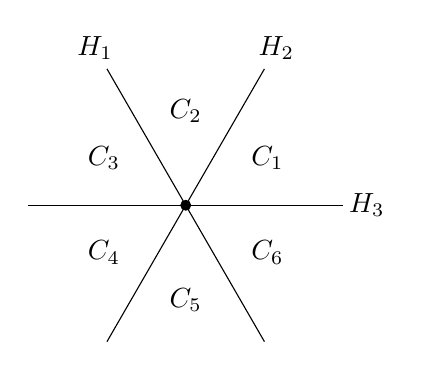
\begin{tikzpicture}
\draw (180:2) -- (0:2);
\draw (60:2) -- (-120:2);
\draw (120:2) -- (-60:2);
\node at (0,0)[circle,fill,inner sep=1.4pt] {};
\node at (120:2.3) {$H_1$};
\node at (60:2.3) {$H_2$};
\node at (0:2.3) {$H_3$};
\node at (30:1.2) {$C_1$};
\node at (90:1.2) {$C_2$};
\node at (150:1.2) {$C_3$};
\node at (210:1.2) {$C_4$};
\node at (270:1.2) {$C_5$};
\node at (330:1.2) {$C_6$};
\end{tikzpicture}\]
and let $W$ be its Weyl group. If we denote by $\{s,\tilde{s}\}$ the orbit of $W$ in $X(W)$ and set $s(C_1)=s_{H_2}$ and $\tilde{s}(C_1)=s_{H_3}$, then
\begin{alignat*}{9}
s(C_1)&=s_{H_2}&\quad& s(C_2)&=s_{H_2}&\quad&s(C_3)&=s_{H_3}&\quad &s(C_4)&=s_{H_3}&\quad&s(C_5)&=s_{H_1}&\quad&s(C_6)&=s_{H_1}\\
\tilde{s}(C_1)&=s_{H_3}&\quad& \tilde{s}(C_2)&=s_{H_1}&\quad&\tilde{s}(C_3)&=s_{H_1}&\quad &\tilde{s}(C_4)&=s_{H_2}&\quad&\tilde{s}(C_5)&=s_{H_2}&\quad&\tilde{s}(C_6)&=s_{H_3}
\end{alignat*}
With this, we see the Coxeter matrix of $W$ is given by
\[M(W)=\begin{pmatrix}
1&3\\
3&1
\end{pmatrix}\]
We then recognize that this matrix is the Coxeter matrix of $\mathfrak{S}_2$, as in Example~\ref{Coxeter group A_n graph}.
\end{example}
\begin{proposition}\label{reflection group Coexter matrix angle prop}
Let $C$ be a chamber and let $i,j\in I$ with $i\neq j$. Put $s_i=s_i(C)$, $H_i=H_i(C)$, $e_i=e_i(C)$ and define $s_j$, $H_j$, and $e_j$ similarly.
\begin{itemize}
\item[(a)] If $H_i$ and $H_j$ are parallel, then $m_{ij}=\infty$ and $e_i=-e_j$.
\item[(b)] If $H_i$ and $H_j$ are not parallel, then $m_{ij}$ is finite and
\begin{align}\label{reflection group Coexter matrix angle prop-1}
(e_i,e_j)=-\cos(\pi/m_{ij}).
\end{align}
In particular, we have $(e_i,e_j)\leq 0$.
\end{itemize}
\end{proposition}
\begin{proof}
If $H_i$ and $H_j$ are parallel, then $s_is_j$ is a translation, so $m_{ij}=\infty$. Moreover, $e_i=\pm e_j$. Now, there exists a point $a$ (resp. $b$) in the closure of $C$ that belongs to $H_i$ (resp. $H_j$) but not to $H_j$ (resp. $H_i$). Then $(a-b,e_i)>0$ and $(b-a,e_j)>0$, which excludes the case $e_i=e_j$ and proves (a).\par
Assume now that $H_i$ and $H_j$ are not parallel. Choose an origin $a\in H_i\cap H_j$ and identify $T$ with $E$ by the bijection $t\mapsto a+t$. Let $V$ be the plane orthogonal to $H_i\cap H_j$ and passing through $a$. Put $\Gamma=V\cap D_{H_i}(C)\cap D_{H_j}(C)$ (where $D_H(C)$ denotes the open half-space bounded by $H$ and containing $C$) and let $D_i$ (resp. $D_j$) be the half-line in $V$ contained in $H_i\cap V$ (resp. $H_j\cap V$) and in the closure of $F$. For a suitable orientation of $V$, the set $F$ is the union of the open half-lines $\Delta$ in $V$ such that
\[0<\widehat{(D,\Delta)}<\widehat{(D_1,D_2)}.\]
Let $\tilde{W}$ be the subgroup of $W$ generated by $s_i$ and $s_j$. For any $w\in\tilde{W}$, the hyperplanes $w(H_i)$ and $w(H_j)$ belong to $\mathcal{H}$, contain $H_i\cap H_j$ and do not meet $C$. It follows that they do not meet $\Gamma$ (\cref{reflection group parallel and chamber}). Then Corollary~\ref{reflection on plane transform not meeting chamber iff} thus implies (b).
\end{proof}
\subsection{Systems of obtuse vectors}
Let $q$ be a positive quadratic form on a real vector space $V$ and let $\beta$ be the associated symmetric bilinear form. A subset $A$ of $V$ is called \textbf{obtuse} with respect to $\beta$ if $\beta(a,b)\leq 0$ for all $a,b\in A$.
\begin{lemma}\label{reflection group obtuse subset linera dependence}
Let $\{a_1,\dots,a_n\}$ be a obtuse subset of $V$ with respect to $\beta$.
\begin{itemize}
\item[(a)] If $c_1,\dots,c_n$ are real numbers such that $q(\sum_ic_ia_i)=0$, then $q(\sum_i|c_i|a_i)=0$.
\item[(b)] If $q$ is non-degenerate and if there exists a linear form $f$ on $V$ such that $f(a_i)>0$ for all $i$, the vectors $a_1,\dots,a_n$ are linearly independent.
\end{itemize} 
\end{lemma}
\begin{proof}
The relation $\beta(a_i,a_j)\leq 0$ for $i\neq j$ immediately implies that
\[q(\sum_i|c_i|a_i)=\sum_{i,j}|c_ic_j|\beta(a_i,a_j)\leq\sum_{i,j}c_ic_j\beta(a_i,a_j)=q(\sum_ic_ia_i),\]
whence (a). If $q$ is non-degenerate, the relation $\sum_ic_ia_i=0$ thus implies that $\sum_i|c_i|a_i=0$; it follows that, for any linear form $f$ on $V$, we have $\sum_i|c_i|f(a_i)=0$, and hence $c_i=0$ for all $i$ if we also have $f(a_i)>0$ for all $i$. This proves (b).
\end{proof}
\begin{lemma}\label{reflection group obtuse symmetric matrix prop}
Let $Q=(q_{ij})$ be a real, symmetric, square matrix of order $n$ such that:
\begin{itemize}
\item[(\rmnum{1})] $q_{ij}\leq 0$ for $i\neq j$;
\item[(\rmnum{2})] there does not exist a partition of $\{1,2,\dots,n\}$ into two non-empty subsets $I$ and $J$ such that $q_{ij}=0$ for $i\in I,j\in J$;
\item[(\rmnum{3})] the quadratic form $q(\bm{x})=\bm{x}^TQ\bm{x}$ induced by $Q$ on $\R^n$ is positive. 
\end{itemize}
Then 
\begin{itemize}
\item[(a)] The kernel $N$ of $q$ is of dimension $0$ or $1$. If $\dim(N)=1$, $N$ is generated by a vector all of whose coordinates are positive.
\item[(b)] The smallest eigenvalue of $Q$ is of multiplicity $1$ and a corresponding eigenvector has all its coordinates positive or all its coordinates negative.
\end{itemize}
\end{lemma}
\begin{proof}
Since $q$ is a positive quadratic form, the kernel $N$ of $q$ is the set of isotropic vectors for $q$. Let $e_1,\dots,e_n$ be the canonical basis of $\R^n$. If $\sum_ic_ie_i\in N$, \cref{reflection group obtuse subset linera dependence} shows that we also have $\sum_i|c_i|e_i\in N$, and hence $\sum_iq_{ij}|c_i|=0$ for all $j$. Let $I$ be the set of $i$ such that $c_i\neq 0$. If $j\notin I$, then $q_{ij}|c_i|<0$ for $i\in I$ (since $i\neq j$) and $q_{ij}|c_i|=0$ for $i\notin I$, so $q_{ij}=0$ for $i\in I$ and all $j$. In particular, assumption (\rmnum{2}) implies that either $I=\emp$ or $I=\{1,\dots,n\}$. Consequently, every non-zero vector in $N$ has nonzero coordinates. If $\dim(N)\geq 2$, the intersection of $N$ with the hyperplane with equation $x_i=0$ would be of dimension $\geq 1$, contrary to what we have just shown. The preceding argument also shows that, if $\dim(N)=1$, then $N$ contains a vector all of whose coordinates are positive. This proves (a).\par
On the other hand, we know that the eigenvalues of $Q$ are real and positive since $q$ is positive. Let $\lambda$ be the smallest of them. The matrix $\tilde{Q}=Q-\lambda I_n$ is then the matrix of a degenerate positive form $\tilde{q}$ and the off-diagonal elements of $\tilde{Q}$ are the same as those of $Q$. Consequently, $\tilde{Q}$ satisfies conditions (\rmnum{1}), (\rmnum{2}) and (\rmnum{3}) of the statement of the lemma. Since the kernel $\tilde{N}$ of $\tilde{q}$ is the eigenspace of $Q$ corresponding to the eigenvalue $\lambda$, assertion (b) follows from (a).
\end{proof}
Now we return to our real affine vector space $E$ and its space of translations $T$. Recall that $\dim(E)=l$ and we have a scalar product on $T$, the results above can be applied to $T$. 
\begin{proposition}\label{reflection group obtuse generating subset prop}
Let $\{e_1,\dots,e_n\}$ be a obtuse subset of $T$ such that
\begin{itemize}
\item[(\rmnum{1})] $\{e_1,\dots,e_n\}$ generates $T$;
\item[(\rmnum{2})] there does not exist a partition of $\{1,\dots,n\}$ into two non-empty subsets $I$ and $J$ such that $(e_i,e_j)=0$ for $i\in I$ and $j\in J$.
\end{itemize}
Then there are two possibilities:
\begin{itemize}
\item[(a)] $(e_1,\dots,e_n)$ is a basis of $T$;
\item[(b)] $n=l+1$, and there exists a family $(c_i)_{1\leq i\leq n}$ of positive real numbers such that $\sum_ic_ie_i=0$, and any family $(\tilde{c}_i)_{1\leq i\leq n}$ of real numbers such that $\sum_i\tilde{c}_ie_i=0$ is proportional to $(c_i)_{1\leq i\leq n}$.
\end{itemize}
\end{proposition}
\begin{proof}
Put $q_{ij}=(e_i,e_j)$. The matrix $Q=(q_{ij})$ then satisfies the hypotheses of \cref{reflection group obtuse symmetric matrix prop}. The kernel $N$ of the quadratic form $q$ on $\R^n$ with matrix $Q$ is the set of $(c_1,\dots,c_n)$ such that $\sum_ic_ie_i=0$. If $N=\{0\}$, the $e_i$ are linearly dependent and we are in case (a). If $\dim(N)=1$, \cref{reflection group obtuse symmetric matrix prop} shows that we are in case (b).
\end{proof}
\begin{proposition}\label{reflection group obtuse basis prop}
Let $(e_1,\dots,e_n)$ be a obtuse basis of $T$.
\begin{itemize}
\item[(a)] If $x=\sum_ic_ie_i$ is such that $(x,e_i)\geq 0$ for all $i$, then $c_i\geq 0$ for all $i$.
\item[(b)] If $x$ and $y$ are two elements of $T$ such that $(x,e_i)\geq 0$ and $(y,e_i)\geq 0$ for all $i$, then $(x,y)\geq 0$. If $(x,e_i)>0$ and $(y,e_i)>0$ for all $i$, then $(x,y)>0$.
\end{itemize}
\end{proposition}
\begin{proof}
Under the hypotheses of (a), assume that $c_i<0$ for some $i$. Let $f$ be the linear form on $T$ defined by $f(e_i)=1$ and $f(e_j)=-c_i/\sum_{k=1}^{n}|c_k|)^{-1}$ for $j\neq i$. The vectors $-x,e_1,\dots,e_n$ then satisfy the hypotheses of \cref{reflection group obtuse subset linera dependence}(b) (taking for $q$ the metric form on $T$). We conclude that they are linearly independent, which is absurd. Hence (a). Moreover, if $x=\sum_ic_ie_i$ and $y\in T$, then $(x,y)=\sum_ic_i(e_i,y)$, so (b) follows immediately from (a).
\end{proof}
\subsection{Finiteness theorems}
\begin{lemma}\label{reflection group inner product leq 1 set finite}
Let $A$ be a set of unit vectors in $T$. If there exists a real number $\lambda<1$ such that $(a,b)\leq\lambda$ for $a,b\in A$ and $a\neq b$, then the set $A$ is finite.
\end{lemma}
\begin{proof}
For $a,b\in A$ such that $a\neq b$, we have
\[\|a-b\|^2=2-2(a,b)\geq 2-2\lambda.\]
Now the unit sphere $S$ of $T$ being compact, there exists a finite covering of $S$ by sets of diameter $<\sqrt{(2-2\lambda)}$ each of these sets contains at most one point of $A$, hence the lemma.
\end{proof}
Denote by $U(w)$ the automorphism of $T$ associated to the affine map $w\in W$ from $E$ to itself. We have
\[w(x+t)=w(x)+U(w)\cdot t\quad\text{for $t\in T$ and $x\in E$}\]
This defines a homomorphism $U$ from the group $W$ to the orthogonal group of $T$; the kernel of $U$ is the set of translations belonging to $W$.
\begin{theorem}\label{reflection group finiteness thm}
Let $U$ be the homomorphism defined above.
\begin{itemize}
\item[(a)] The set of walls of a chamber is finite.
\item[(b)] The set of directions of hyperplanes belonging to $\mathcal{H}$ is finite.
\item[(c)] The group $U(W)$ is finite.
\end{itemize}
\end{theorem}
\begin{proof}
Assertion (a) follows immediately from \cref{reflection group Coexter matrix angle prop}(b) and \cref{reflection group inner product leq 1 set finite}. We prove (b). Let $C$ be a chamber and $\mathcal{W}$ the set of its walls. The facets of $\widebar{C}$ (relative to $\mathcal{H}$) are the same as those relative to $\mathcal{W}$ (\cref{reflection group wall of chamber prop}). Since $\mathcal{W}$ is finite, they are finite in number. Since a facet meets only finitely many hyperplanes belonging to $\mathcal{H}$, the set of hyperplanes belonging to $\mathcal{H}$ and meeting $\widebar{C}$ is finite, hence so is the set $A(C)$ of unit vectors in $T$ orthogonal to some hyperplane belonging to $\mathcal{H}$ and meeting $\widebar{C}$. Consequently, there exists a real number $\lambda<1$ such that $(a,b)\leq\lambda$ for $a,b\in A(C)$ and $a\neq b$.\par
Let $A$ be the set of unit vectors in $T$ orthogonal to a hyperplane belonging to $\mathcal{H}$. Let $a,b\in A$ with $a\neq b$. If $a$ and $b$ are parallel, then $a=-a$ and $(a,b)=-1$. Otherwise, let $H\in\mathcal{H}$ (resp. $L\in\mathcal{H}$) be such that $a$ (resp. $b$) is orthogonal to $H$ (resp. $L$). We have $H\cap L\neq\emp$, and if $x\in H\cap L$ there exists an element $w\in W$ such that $x\in w(\widebar{C})$. The vectors $U(w)\cdot a$ and $U(w)\cdot b$ then belong to $A(C)$, we have 
\[(a,b)=(U(w)\cdot a,U(w)\cdot b)\leq \lambda\]
and the set $A$ is finite by \cref{reflection group inner product leq 1 set finite}. Hence (b).\par
Now let $w\in W$ be such that $U(w)\cdot a=a$ for all $a\in A$. Then $U(w)\cdot t=t$ for all $t$ belonging to the subspace of $T$ generated by $A$. On the other hand, if $t\in T$ is orthogonal to $A$, we have $U(s_H)\cdot t=t$ for all $H\in\mathcal{H}$, hence $U(w)\cdot t=t$ and therefore $U(w)=1$. Since $U(w)(A)=A$ for all $w\in W$, we deduce that $U(W)$ is isomorphic to a group of permutations of the finite set $A$, hence (c).
\end{proof}
\begin{proposition}\label{reflection group subgroup of walls finite iff}
Let $C$ be a chamber and $\mathcal{R}$ a set of walls of $C$. Let $W_{\mathcal{R}}$ be the subgroup of $W$ generated by the orthogonal reflections with respect to the elements of $\mathcal{R}$. For $H\in\mathcal{R}$, denote by $e_H$ the unit vector orthogonal to $H$ on the same side of $H$ as $C$. Then the following conditions are equivalent:
\begin{itemize}
\item[(\rmnum{1})] The group $W_{\mathcal{R}}$ is finite.
\item[(\rmnum{2})] There exists a point of $E$ invariant under every element of $W_{\mathcal{R}}$. 
\item[(\rmnum{3})] The hyperplanes belonging to $\mathcal{R}$ have non-empty intersection.
\item[(\rmnum{4})] The family of vectors $(e_H)_{H\in\mathcal{R}}$ is free in $T$.
\end{itemize}
\end{proposition}
\begin{proof}
If $W_{\mathcal{R}}$ is finite, then the element $\sum_{w\in W_{\mathcal{R}}}w(x)$ is invariant under $W_{\mathcal{R}}$, so $W_{\mathcal{R}}$ has a fixed point. Converselt, by property (D2) at the beginning of this paragraph, the stabiliser in $W$ of every point of $E$ is finite, so (\rmnum{2}) implies (\rmnum{1}).\par
Since the group $W_{\mathcal{R}}$ is generated by the set of reflections with respect to the hyperplanes belonging to $\mathcal{R}$, the fixed points of $W_{\mathcal{R}}$ are the points of $E$ belonging to every hyperplane $H\in\mathcal{R}$, hence the equivalence of (\rmnum{2}) and (\rmnum{3}).\par
Assume that there exists a point $a$ of $E$ such that $a\in H$ for all $H\in\mathcal{R}$ and let $t\in T$ be such that $a+t\in C$. Since $(e_{H_1},e_{H_2})\leq 0$ for $H_1,H_2\in\mathcal{R}$ such that $H_1\neq H_3$ (\cref{reflection group Coexter matrix angle prop}), and since $(t,e_H)>0$ for all $H\in\mathcal{R}$, \cref{reflection group obtuse subset linera dependence}(b) implies that the $e_H$ for $H\in\mathcal{R}$ are linearly independent. Consequently, (\rmnum{3}) implies (\rmnum{4}).\par
Suppose finally that the family $(e_H)_{H\in\mathcal{R}}$ is free. Let $a$ be a point of $E$. For any hyperplane $H\in\mathcal{R}$, there exists a real number $c_H$ such that $H$ consists of the points $a+t$ of $E$ with $(t,e_H)=c_H$. Since the family $(e_H)$ is free, there exists $t\in T$ such that $(t,e_H)=c_H$ for all $H\in\mathcal{R}$, and the point $a+t$ of $E$ belongs to all the hyperplanes $H\in\mathcal{R}$. Thus, (\rmnum{4}) implies (\rmnum{3}).
\end{proof}
\begin{remark}
Since $W$ is generated by reflections with respect to the walls of the chamber $C$, the preceding proposition gives a criterion for $W$ to be finite. We shall return to this question later.
\end{remark}
\begin{example}
Let $F$ be a finite-dimensional real affine space and $G$ a group of automorphisms of $F$. For all $g\in G$, denote by $U(g)$ the automorphism of the space of translations $V$ of $F$ associated to $g$. Assume that the image $U(G)$ is a finite subgroup of $\GL(V)$; then $V$ has a scalar product invariant under $U(G)$. If, in addition, $G$ acts properly on $F$ when it is provided with the discrete topology, and if it is generated by reflections, we can apply to $G$ the results of this paragraph.
\end{example}
\subsection{Representation of the Weyl group on the underlying space}
Let $I$ be the set of vertices of the Coxeter graph of $W$ and let $J$ be a subset of $I$ such that no vertex in $J$ is linked to any vertex in $I\setminus J$. Ley $C$ be a chamber, $s$ the canonical bijection from $I$ to the set of reflections with respect to the walls of $C$, and let $W_{J,C}$ be the subgroup generated by the image $s(J)$. It follows from \cref{Coxeter system restricted product if} that $W$ is the direct product of the two subgroups $W_{J,C}$ and $W_{I\setminus J,C}$. Let $\tilde{C}$ be another chamber and $\tilde{s}$ the corresponding injection of $I$ into $W$. We have seen that if $w\in W$ transforms $C$ into $\tilde{C}$, then $\tilde{s}(i)=ws(i)w^{-1}$ for $i\in I$. Since $W_{J,C}$ is normal in $W$, it follows that $\tilde{s}(i)\in W_{J,C}$ for all $i\in J$. We deduce that the subgroup $W_{J,C}$ does not depend on $C$. We denote it simply by $W_J$ from now on.
\begin{remark}
The definition of $W_{J,C}$ clearly extends to an arbitrary subset $J$ of $I$. But if there exist a vertex in $J$ and a vertex in $I\setminus J$ that are linked, then $W_{J,C}$ is not normal and depends on the choice of $C$.
\end{remark}
Let $T_J$ be the subspace of $T$ consisting of the vectors invariant under every element of $U(W_J)$ and let $T_J^\bot$ be the subspace orthogonal to $T_J$. Since $W_J$ is a normal subgroup of $W$, it is clear that $T_J$ is invariant under $U(W)$, and hence so is $T_J^\bot$.
\begin{proposition}\label{reflection group representation on translation space prop}
Let $J_1,\dots,J_r$ be the sets of vertices of the connected components of the Coxeter graph of $W$. For $1\leq p\leq r$, put
\[W_p=W_{J_p},\quad T_p=T_{J_p},\quad T_p^\bot=T_{J_p}^\bot,\quad\text{and}\quad T_0=\bigcap_{p=1}^{r}T_p.\]
\begin{itemize}
\item[(a)] The group $W$ is the direct product of the groups $W_p$.
\item[(b)] The space $T$ is the orthogonal direct sum of the subspaces $T_0,T_1^\bot,\dots,T_r^\bot$, which are all stable under $U(W)$.
\item[(c)] For all $q$, the subspace $T_q$ of $T$ consists of the vectors invariant under $U(W_q)$; it is the direct sum of the $T_p^\bot$ for $p\neq q$.
\item[(d)] Let $C$ be a chamber. The subspace $T_p^\bot$ is generated by the vectors $e_i(C)$ for $i\in J_p$.
\item[(e)] The representations of $W$ in the subspaces $T_p^\bot$ are absolutely irreducible, non-trivial, and pairwise inequivalent. 
\end{itemize}
\end{proposition}
\begin{proof}
Assertion (a) follows from \cref{Coxeter system restricted product if}. On the other hand, we have already seen that the subspaces $T_p^\bot$, are invariant under $U(W)$, and so is $T_0$. Let $C$ be a chamber; since $W_p$ is generated by the reflections $s_i(C)$ for $i\in J_p$, it is clear that $T_p$ is the subspace orthogonal to the $e_i(C)$ (which we simply denote by $e_i$ henceforth) for $i\in J_p$, hence (d). Moreover, if $i\in J_p$, $j\in J_q$ with $p\neq q$, then $m_{ij}=2$ since $\{i,j\}$ is not an edge of the Coxeter graph of $W$, so $(e_i,e_j)=0$. Assertion (b) is now immediate. And assertion (c) follows, since $T_p$ is the orthogonal complement of $T_p^\bot$.\par
Finally, let $V$ be a subspace of $T_p^\bot$ invariant under $U(W_p)$. For all $i\in J_p$, either $e_i\in V$ is orthogonal to $V$ (\cref{reflection invariant subspace endo iff}). Let $A$ (resp. $B$) be the set of $i\in J_p$ such that $e_i\in V$ (resp. $e_i$ is orthogonal to $V$). Clearly $(e_i,e_j)=0$ for $i\in A$ and $j\in B$, and since $J_p$ is the vertices of a connected component of the Coxeter graph, it follows that either $A=\emp$ and $V=\{0\}$, or $A=J_p$ and $V=T_p^\bot$. Consequently, the representation of $W_p$ on $T_p^\bot$ is irreducible, hence absolutely irreducible (\cref{pseudo-reflection and irreducible representation}). It is non-trivial by the very definition of $T_p^\bot$. Finally, the last assertion in (e) follows immediately from (c).
\end{proof}
If the subspace $T_0$ of vectors in $T$ invariant under $U(W)$ reduces to $\{0\}$, then $W$ is said to be \textbf{essential}; if the representation $U$ of $W$ on $T$ is irreducible, then $W$ is said to be \textbf{irreducible}.
\begin{corollary}
Assume that $W\neq\{1\}$. Then $W$ is irreducible if and only if it is essential and its Coxeter graph is connected.
\end{corollary}
We retain the notation of \cref{reflection group representation on translation space prop}. For $1\leq p\leq r$, let $E_p$ be the set of orbits of the group $T_p$ in $E$, and let $\pi_p$ be the canonical map from $E$ to $E_p$. Moreover, let $E_0$ be the set of orbits of $T_0^\bot$. The action of $T$ on $E$ passes to the quotient; in particular, $T_p^\bot$ acts on $E_p$ and it is immediate (for example by taking an origin in $E$) that $E_p$ is an affine space admitting $T_p^\bot$ as its space of translations. Put $\tilde{E}=E_0\times E_1\times\cdots\times E_r$; this is an affine space having $T=T_0\oplus T_1^\bot\oplus\cdots\oplus T_r^\bot$ as its space of translations. Let $\pi:E\to\tilde{E}$ be the product map of the $\pi_p$; since $\pi$ commutes with the action of $T$, this is a bijection and even an isomorphism of affine spaces. In what follows, we identify $E$ and $\tilde{E}$ by means of $\pi$; the map $\pi_p$ is then identified with the canonical projection of $\tilde{E}$ onto $E_p$.\par
Since $W$ leaves $T_p$ stable, the action of $W$ on $E$ passes to the quotient and defines an action of $W$ on $E_p$, and hence by restriction an action of $W_p$ on $E_p$. On the other hand, let $C$ be a chamber, let $i\in I$ and let $p$ be the integer such that $i\in J_p$. For any $x\in E$, we have
\[s_i(C)(x)=x-\lambda e_i(C)\quad\text{with}\quad\lambda\in\R.\]
Since $e_i\in T_q$ for $q\neq p$, it follows that $\pi_q(w(x))=\pi_q(x)$ for $x\in E$, $w\in W_p$ and $q\neq p$. Consequently, if $w=w_1\cdot w_r$ with $w_p\in W_p$ for $1\leq p\leq r$, then
\begin{align}\label{reflection group action on affine space is product}
w(x_0,\dots,x_r)=(x_0,w_1(x_1),\dots,x_r(x_r))
\end{align}
for all $x_p\in E_p$ and $0\leq p\leq r$. In other words, the action of $W$ on $E$ is exactly the product of the actions of the $W_p$ on $E$ (we put $W_0=\{1\}$). It follows that $W_p$ acts faithfully on $E_p$ and that $W_p$ can be identified with a group of displacements of the Euclidean space $E_p$ (the space $T_p^\bot$ of translations of $E_p$ being provided, of course, with the scalar product induced by that on $T$).
\begin{proposition}\label{reflection group decomposition of affine space}
Assume the notations in \cref{reflection group representation on translation space prop}.
\begin{itemize}
\item[(a)] The group $W_p$ is a group of displacements of the Euclidean affine space $E_p$; it is generated by reflections; provided with the discrete topology, it acts properly on $E_p$; it is irreducible.
\item[(b)] Let $\mathcal{H}_p$ be the set of hyperplanes $H$ of $E_p$ such that $s_H\in W_p$. The set $\mathcal{H}$ consists of the hyperplanes of the form
\[H=E_0\times E_1\times\cdots\times E_{p-1}\times H_p\times E_{p+1}\times\cdots E_r\] 
with $1\leq p\leq r$ and $H_p\in\mathcal{H}_p$.
\item[(c)] Every chamber $C$ is of the form $E_0\times C_1\times\cdots\times C_p$, where for each $p$ the set $C_p$ is a chamber defined in $E_p$ by the set of hyperplanes $\mathcal{H}_p$; moreover, the walls of $C_p$ are the hyperplanes $\pi_p(H_i(C))$ for $i\in J_p$.
\end{itemize}
\end{proposition}
\begin{proof}
Let $C$ be a chamber. Put $H_i=H_i(C)$, $e_i=e_i(C)$ and $s_i=s_i(C)$ for $i\in I$. Let $i$ be in $J_p$. Since $e_i\in T_p^\bot$ and $T$ is the direct sum of the mutually orthogonal subspaces $T_0,T_1^\bot,\dots,T_r^\bot$, the hyperplane of $T$ orthogonal to $e_i$ is of the form $L_i+T_p$, where $L_i$ is the hyperplane of $T_p^\bot$ orthogonal to $e_i$. The affine hyperplane $H_i$ of $E$ is of the form $L_i+T_p+x$, with $x\in E$, and we have
\begin{align}\label{reflection group decomposition of affine space-1}
H_i=E_0\times E_1\times\cdots\times E_{p-1}\times\tilde{H}_i\times E_{p+1}\times\cdots\times E_r
\end{align}
with $\tilde{H}_i=L_i+\pi_p(x)=\pi_p(H_i)$. It is now immediate that $s_i$ acts in $E_p$ by the reflection associated to the hyperplane $\tilde{H}_i$ of $E_p$. Thus, the group $W_p$ is a group of displacements generated by reflections in $E_p$; the verification of the properness criterion (D2') is immediate. Finally, \cref{reflection group representation on translation space prop}(e) shows that $W_p$ is irreducible. This proves (a).\par
By Corollary~\ref{reflection group generator conjugation prop}, the set $\mathcal{H}_p$ consists of the hyperplanes of the form $w_p(\tilde{H}_i)$ for $i\in J_p$ and $w\in W_p$. Further, if $w=w_1\cdots w_r$ with $w_p\in W_p$ for all $p$, formulas (\ref{reflection group action on affine space is product}) and (\ref{reflection group decomposition of affine space-1}) imply that
\begin{align}\label{reflection group decomposition of affine space-2}
w(H_i)=E_0\times E_1\times\cdots\times E_{p-1}\times w_p(\tilde{H}_i)\times E_{p+1}\times\cdots\times E_r
\end{align}
from which (b) follows immediately.\par
Let $i\in J_p$. By formula (\ref{reflection group decomposition of affine space-2}), the open half-space $D_i$ bounded by $H_i$ and containing $C$ is of the form
\[D_i=E_0\times E_1\times\cdots\times E_{p-1}\times\tilde{D}_i\times E_{p+1}\times\cdots\times E_r\]
Where $\tilde{D}_i$ is an open half-space bounded by $\tilde{H}_i$ in $E_p$. Put $C_p=\bigcap_{i\in J_p}\tilde{D}_i$; since $C=\bigcap_{i\in I}D_i$, it follows immediately that
\[C=E_0\times C_1\times\cdots\times C_r\]
consequently, none of the sets $C_p$ is empty, and since $C$ does not meet any hyperplane belonging to $\mathcal{H}$, the set $C_p$ does not meet any hyperplane belonging to $\mathcal{H}_p$. \cref{reflection group chamber if} now shows that $C_p$ is one of the chambers defined by $\mathcal{H}_p$ in $E_p$. By using \cref{reflection group affine intersection of hyperplanes prop}, it is easy to see that the walls of $C_p$ are the hyperplanes $\tilde{H}_i=\pi_p(H_i)$ for $i\in J_p$.
\end{proof}
\subsection{Structure of chambers}
Let $C$ be a chamber, let $\mathcal{W}$ be the set of walls of $C$, and for $H\in\mathcal{W}$ let $e_H$ be the unit vector orthogonal to $H$ on the same side of $H$ as $C$.
\begin{proposition}\label{reflection group essential finite chamber prop}
Assume that the group $W$ is essential and finite. Then:
\begin{itemize}
\item[(a)] There exists a unique point $a$ of $E$ invariant under $W$.
\item[(b)] The family $(e_H)_{H\in\mathcal{W}}$ is a basis of $T$.
\item[(c)] The chamber $C$ is the open simplicial cone with vertex $a$ defined by the dual basis of $(e_H)_{H\in\mathcal{W}}$ in $T$.
\end{itemize}
\end{proposition}
\begin{proof}
By \cref{reflection group subgroup of walls finite iff}, there exists a point $a\in E$ invariant under $W$. Let $t\in T$ be such that $t+a$ is invariant under $W$. For all $w\in W$,
\[U(w)\cdot t+a=w(t+a)=t+a\]
so $U(w)\cdot t=t$. Since $W$ is essential, this implies that $t=0$, showing the uniqueness of $a$.\par
Since $W$ is essential, $T_0=\{0\}$ in the notation of \cref{reflection group representation on translation space prop}, and \cref{reflection group representation on translation space prop} shows that the family $(e_H)_{H\in\mathcal{W}}$ generates the vector space $T$. The existence of a point of $E$ invariant under $W$ shows that the family $(e_H)_{H\in\mathcal{W}}$ is free (\cref{reflection group subgroup of walls finite iff}).\par
Let $a$ be the unique point of $E$ invariant under $W$. Since $(e_H)_{H\in\mathcal{W}}$ is a basis of $T$, and since the scalar product is a non-degenerate bilinear form on $T$, there exists a unique basis $(f_H)_{H\in\mathcal{W}}$ of $T$ such that $(e_H,f_L)=\delta_{H,L}$ for $H,L$ in $\mathcal{W}$. Every point $x$ of $E$ can be written uniquely in the form $x=t+a$ with $t=\sum_{H}\xi_H f_H$. Then $x$ belongs to $C$ if and only if, for every hyperplane $H\in\mathcal{W}$, $x$ is on the same side of $H$ as $e_H$, or in other words $(t,e_H)=\xi_H$ is strictly positive. Hence (c).
\end{proof}
\begin{proposition}\label{reflection group essential infinite chamber prop}
Assume that the group $W$ is essential, irreducible and infinite. Then:
\begin{itemize}
\item[(a)] No point of $E$ is invariant under $W$.
\item[(b)] We have $|\mathcal{W}|=\dim(T)+1$, and there exist real numbers $c_H>0$ such that $\sum_Hc_He_H=0$. Moreover, any family $(\tilde{c}_H)_{H\in\mathcal{W}}$ of real numbers such that $\sum_H\tilde{c}_He_H=0$ is proportional to $(c_H)_{H\in\mathcal{W}}$. 
\item[(c)] The chamber $C$ is an open simplex.
\end{itemize}
\end{proposition}
\begin{proof}
Assertion (a) follows from \cref{reflection group subgroup of walls finite iff}. On the other hand, since $W$ is essential, the vectors $(e_H)_{H\in\mathcal{W}}$ generate $T$. We have $(e_H,e_{\tilde{H}})\leq 0$ for $H,\tilde{H}\in\mathcal{H}$ and $H\neq\tilde{H}$ (\cref{reflection group Coexter matrix angle prop}) and, since $W$ is irreducible, there does not exist a partition of $\mathcal{W}$ into two disjoint subsets $\mathcal{W}_1$ and $\mathcal{W}_2$ such that $H_1\in\mathcal{W}_1$ and $H_2\in\mathcal{W}_2$ imply that $e_{H_1},e_{H_2})=0$. We can thus apply \cref{reflection group obtuse generating subset prop} and case (a) of that lemma is excluded; indeed, the $e_H$ are not linearly independent, since $W$ has no fixed point. Assertion (b) follows.\par
We now prove (c). Number the walls of $C$ as $H_0,H_1,\dots,H_l$ and put $t_i=e_{H_i}$. By (b), the vectors $t_1,\dots,t_l$ form a basis of $T$, so the hyperplanes $H_1,\dots,H_l$ have a point $a_0$ in common, and there exists a basis $(t_1^*,\dots,t_l^*)$ of $T$ such that $(t_i,t_j^*)=\delta_{ij}$. Moreover, again by (b) there exist positive real numbers $c_1,\dots,c_l$ such that 
\[t_0=-(c_1t_1+\cdots+c_lt_l).\]
Since the vector $t_0$ is orthogonal to the hyperplane $H_0$, there exists a real number $c$ such that $H_0$ is the set of points $x=t+a_0$ of $E$ with $(t,t_0)=-c$.\par
Every point of $E$ can be written uniquely in the form $x=t+a_0$ with $t=\xi_1t_1^*+\cdots+\xi_lt_l^*$ and $\xi_1,\dots,\xi_l$ real. The point $x$ belongs to $C$ if and only if it is on the same side of $H_i$ as $t_i$ for $0\leq i\leq l$; this translates into the inequalities $(t,t_i)>0$ for $1\leq i\leq l$ and $(t,t_0)>-c$, or equivalently by $\xi_i>0$ for $1\leq i\leq l$ and $c_1\xi_1+\cdots+c_l\xi_l<c$. Since $C$ is non-empty, we therefore have $c>0$. Put $a_i=a_0+\frac{c}{c_i}t_i^*$ for $1\leq i\leq l$. Then the chamber $C$ consists of the $l$ points of $E$ of the form $a_0+\sum_{i=1}^{l}\lambda_i(a-a_0)$ with $\lambda_i>0$ and $\lambda_1+\cdots+\lambda_l<1$, so $C$ is the open simplex with vertices $a_0,\dots,a_l$.
\end{proof}
\begin{remark}
Identify $E$ with $E_0\times E_1\times\cdots E_r$ and $W$ with $W_1\times\cdots\times W_r$. By \cref{reflection group decomposition of affine space}, the chamber $C$ is then identified with $E_0\times C_1\times\cdots\times C_r$ where $C_p$ is a chamber in $E_p$ with respect to the set of hyperplanes $\mathcal{H}_p$. By \cref{reflection group essential finite chamber prop} and \cref{reflection group essential infinite chamber prop}, each of the chambers $C_p$ is an open simplicial cone or an open simplex.
\end{remark}
\begin{remark}
Assume that $W$ is irreducible and essential. If $H_1$ and $H_2$ are two walls of $C$, then $m_{H_1,H_2}$ if and only if $e_{H_1}=-e_{H_2}$ (\cref{reflection group Coexter matrix angle prop}). By \cref{reflection group essential finite chamber prop} and \cref{reflection group essential infinite chamber prop}, this can happen only if $H_1$ and $H_2$ are the only walls of $C$ and $E$ is of dimension $1$. Thus, the only case in which one of the $m_{H_1,H_2}$ is infinite is that in which $E$ is of dimension $1$ and the group $W$ is generated by the reflections associated to two distinct points.\par
In the general case, the entries of the Coxeter matrix associated to $W$ are finite unless at least one of $E_1,\dots,E_r$ is of the preceding type.
\end{remark}
\subsection{Special points}
Let $W_T$ be the set of translations belonging to $W$ and let $\Lambda$ be the set of $t\in T$ such that the translation $x\mapsto x+t$ belongs to $W_T$. It is immediate that $\Lambda$ is stable under $U(W)$ and that $W_T$ is a normal subgroup of $W$. Since $W$ acts properly on $E$, the same holds for $W_T$, and it follows easily that $\Lambda$ is a discrete subgroup of $T$. For any point $x$ of $E$, denote by $W_x$ the stabiliser of $x$ in $W$.
\begin{proposition}\label{reflection group special point iff}
Let $x\in E$. The following conditions are equivalent:
\begin{itemize}
\item[(\rmnum{1})] We have $W=W_x\cdot W_T$.
\item[(\rmnum{2})] The restriction of the homomorphism $U$ to $W_x$ is an isomorphism from $W_x$ to $U(W)$.
\item[(\rmnum{3})] For every hyperplane $H\in\mathcal{H}$, there exists a hyperplane $\tilde{H}\in\mathcal{H}$ parallel to $H$ and such that $x\in\mathcal{H}$.
\end{itemize}
\end{proposition}
\begin{proof}
It is clear that (\rmnum{1})$\Leftrightarrow$(\rmnum{2}), since $W_T$ is the kernel of $U$ and $W_T\cap W_x=\{1\}$. Assume (\rmnum{1}) and let $H\in\mathcal{H}$; then $s_H\in W_x\cdot W_T$ so there exists a vector $t\in\Lambda$ such that $x=s_H(x)+t$. The vector $t$ is therefore orthogonal to $H$, and if $\tilde{H}=H+\frac{1}{2}t$ then $s_{\tilde{H}}(x)=s_H(x)+t$ for all $x\in E$. Since $t\in\Lambda$ and $s_H\in W$, we have $s_{\tilde{H}}\in W$, and so $\tilde{H}\in\mathcal{H}$; we also have $x=s_{\tilde{H}}(x)$, and so $x\in\tilde{H}$. Thus, (\rmnum{1}) implies (\rmnum{3}).\par
Assume (\rmnum{3}). Let $H\in\mathcal{H}$, take $\tilde{H}$ as in (\rmnum{3}). Then $s_{\tilde{H}}(x)=x$, so $s_{\tilde{H}}\in W_x$. Since $H$ is parallel to $\tilde{H}$, the element $w=s_{\tilde{H}}s_H$ of $W$ is a translation, so $w\in W_T$; then $s_H=s_{\tilde{H}}w\in W_x\cdot W_T$. Since $W$ is generated by the family $(s_H)_{H\in\mathcal{H}}$, it follows that $W=W_x\cdot W_T$ and hence (\rmnum{3}) implies (\rmnum{1}).
\end{proof}
A point $x$ of $E$ is called \textbf{special} for $W$ if it satisfies the equivalent conditions in \cref{reflection group special point iff}. It is clear that the set of special points of $E$ is stable under $W$.
\begin{proposition}
There exists a special point for $W$.
\end{proposition}
\begin{proof}
By \cref{reflection group representation on translation space prop}, we need only consider the case when $W$ is essential. The group $U(W)$ of automorphisms of $T$ is finite (\cref{reflection group finiteness thm}) and $U(s_H)$ is an orthogonal reflection for every hyperplane $H$; moreover, $U(W)$ is generated by the family $(U(s_H))_{H\in\mathcal{H}}$. By \cref{reflection group essential finite chamber prop}, there exists a basis $(e_i)_{i\in I}$ of $T$ such that the group $U(W)$ is generated by the set of reflections $(s_i)_{i\in I}$ defined by
\[s_i(t)=t-2(t,e_i)e_i\]
The Corollary~\ref{reflection group generator conjugation prop} shows that every reflection $s\in U(W)$ is of the form $s=U(s_H)$ with $H\in\mathcal{H}$. We can thus find in $\mathcal{H}$ a family of hyperplanes $(H_i)_{i\in I}$ such that $s_i=U(s_{H_i})$ for all $i$. Since the vectors $e_i$ are linearly independent, there exists $x\in E$ such that $x\in H_i$ for all $i\in I$ (\cref{reflection group subgroup of walls finite iff}). We have $s_{H_i}\in W_x$, so $U(W)=U(W_x)$, which means that $W=W_x\cdot W_T$ since $W_T$ is the kernel of $U$. Thus, $x$ is a special point.
\end{proof}
\begin{remark}
When $W$ is finite and essential, there is only one special point for $W$, namely the unique point invariant under W. Thus, the consideration of special points is interesting mainly when $W$ is infinite.
\end{remark}
\begin{proposition}\label{reflection group special point defined chamber prop}
Assume that $W$ is essential. Let $x$ be a special point for $W$. Then the chambers relative to $W_x$ are the open simplicial cones with vertex $x$. For every chamber $C_x$ relative to $W_x$, there exists a unique chamber $C$ relative to $W$ contained in $C_x$ and such that $x\in\widebar{C}$. The union of the $\tilde{w}(\widebar{C})$ for $\tilde{w}\in W_x$ is a closed neighbourhood of $x$ in $E$. Every wall of $C_x$ is a wall of $C$. If $W$ is infinite and irreducible, the walls of $C$ are the walls of $C_x$ together with an affine hyperplane not parallel to the walls of $C_x$.
\end{proposition}
\begin{proof}
Let $\mathcal{H}_x$ be the set of $H\in\mathcal{H}$ containing $x$. The group $W_x$ is generated by the $H$ for $H\in\mathcal{H}_x$ \cref{reflection group generated by subset char}). The chambers relative to $W_x$ are the open simplicial cones with vertex $x$ (\cref{reflection group essential finite chamber prop}). Let $C_x$ be such a chamber and let $U$ be a non-empty open ball with centre $x$ not meeting any element of $\mathcal{H}\setminus\mathcal{H}_x$. Since $x\in\widebar{C}_x$, there exists a point $y$ in $U\cap C_x$. Then $y\notin H$ for all $H\in\mathcal{H}$, so $y$ belongs to a chamber $C$ relative to $\mathcal{H}$. Since $\mathcal{H}_x\sub\mathcal{H}$, we have $C\sub C_x$. The set $U\cap C_x$ does not meet any $H\in\mathcal{H}$ and is convex, so $U\cap C_x\sub C$; thus $x\in C$. Conversely, let $C_1$ be a chamber relative to $W$ contained in $C_x$ and such that $x\in\widebar{C}_1$; then $C_1$ meets $U$ and $U\cap C_1\sub U\cap C_x=U\cap C$; the chambers $C$ and $C_1$, having a point in common, must coincide. For any $\tilde{w}\in W_x$, we have $\tilde{w}(U)=U$, so
\[U\cap\tilde{w}(C)=\tilde{w}(U\cap C)=\tilde{w}(U\cap C_x)=U\cap\tilde{w}(C_x).\]
Since the union of the $\tilde{w}(C_x)$ for $\tilde{w}\in W_x$ is dense in $E$, the union of the $U\cap\tilde{w}(C)=U\cap\tilde{w}(C_x)$ is dense in $U$, and the union of the $\tilde{w}(\widebar{C})$ for $\tilde{w}\in W_x$ thus contains $U$. Finally, if $H$ is a wall of $C_x$, there exist a point $z\in U\cap H$ and an open neighbourhood $V\sub U$ of $z$ such that $V\cap C_x$ is the intersection of $V$ and the open half-space bounded by $H$ containing $C_x$; since $V\cap C_x=V\cap U\cap C_x=V\cap U\cap C=V\cap C$, it follows that $H$ is awall of $C$. If $W$ is infinite and irreducible, $C$ is an open simplex by \cref{reflection group essential infinite chamber prop} and so has one more wall than the open simplicial cone $C_x$.
\end{proof}
\begin{corollary}\label{reflection group special point and vertex of chamber}
Assume that $W$ is essential.
\begin{itemize}
\item[(a)] If $x\in E$ is special, there exists a chamber $C$ such that $x$ is an extremal point of $C$.
\item[(b)] If $C$ is a chamber, there exists an emtremal point of $C$ that is special.
\end{itemize}
\end{corollary}
\begin{proof}
The first assertion follows from \cref{reflection group special point defined chamber prop}. The second follows from the first and the fact that $W$ acts transitively on the set of chambers.
\end{proof}
\begin{remark}
Assume that $W$ is essential, irreducible and infinite and retain the notation of \cref{reflection group special point defined chamber prop}. Since $U$ is an isomorphism from $W_x$ to $U(W)$, it follows that the Coxeter graph of the group of displacements $U(W)$ (which is generated by the reflections $U(s_H)$ for $H\in\mathcal{H}$ can be obtained from the Coxeter graph of $W$ by omitting the vertex $i$ corresponding to the unique wall of $C$ that is not a wall of $C_x$.
\end{remark}
\begin{proposition}\label{reflection group special point under translation}
Assume that $W$ is essential. Let $x$ be a special point, $\Omega_x$ be the set of its transforms under the group of translations $W_T$, and let $C$ be a chamber. Then $C$ meets $\Omega_x$ in a unique point, which is an extremal point of $C$.
\end{proposition}
\begin{proof}
There exists a chamber $C_0$ such that $x$ is an extremal point of $C_0$ (Corollary~\ref{reflection group special point and vertex of chamber}). Every chamber is of the form $C=t\tilde{w}(C_0)$ with $\tilde{w}\in W_x$ and $t\in W_T$ since $W=W_x\cdot W_T$. Thus $t\tilde{w}(x)=t(x)\in \Omega_x$ is an extremal point of $C$. On the other hand, $C$ cannot contain two distinct points of $\Omega_x$ since $C$ is a fundamental domain for $W$.
\end{proof}
\begin{remark}
The set $\Omega_x$ is contained in the set of special points, but in general is distinct from it.
\end{remark}
\section{Geometric representation of a Coxeter matrix}
In this section, all vector spaces will be assumed to be real.
\subsection{Associated form and reflections of a Coxeter matrix}
Let $S$ be a set and let $M=(m(s,\tilde{s}))$ be a Coxeter matrix of type $S$. Let $E$ be the real vector space spanned by $S$, $(e_s)_{s\in S}$ be the canonical basis of $E$, and let $\beta_M$ be the bilinear form on $E$ such that
\[\beta_M(e_s,e_{\tilde{s}})=-\cos\frac{\pi}{m(s,\tilde{s})}.\]
The form $\beta_M$ is symmetric. It is called the associated form of the matrix $M$. We have $\beta_M(s,s)=1$ and $\beta_M(s,\tilde{s})\leq 0$ for $s,\tilde{s}\in S$ and $s\neq\tilde{s}$. Let $s\in S$ and let $f_s$ be the linear form $x\mapsto 2\beta_M(e_s,x)$. We denote by $\sigma_s$ the pseudo-reflection defined by the pair $(e_s,f_s)$; since $(e_s,f_s)=2$, it is a reflection. We have
\[\sigma_s(x)=x-2\beta_M(e_s,x)e_s\]
and in particular
\[\sigma_s(e_{\tilde{s}})=e_{\tilde{s}}-2\cos\frac{\pi}{m(s,\tilde{s})}e_s.\]
Since $e_s$ is not isotropic for $\beta_M$, the space $E$ is the direct sum of the line $\R e_s$ and the hyperplane $H_s$ orthogonal to $e_s$. Since $\sigma_s$ is equal to $-1$ on $\R e_s$ and to $1$ on $H_s$, it follows that $\sigma_s$ preserves the form $\beta_M$. When $S$ is finite and $\beta_M$ is non-degenerate (a case to which we shall examine), it follows that $\sigma_s$ is an orthogonal reflection.\par
Now let $s,\tilde{s}\in S$ with $s\neq\tilde{s}$, and denote by $E_{s,\tilde{s}}$ the plane $\R e_s\oplus\R e_{\tilde{s}}$.
\begin{proposition}\label{Coxeter matrix form non-dege iff finite}
The restriction of $\beta_M$ to $E_{s,\tilde{s}}$ is positive, and it is nondegenerate if and only if $m(s,\tilde{s})$ is finite.
\end{proposition}
\begin{proof}
Let $z=xe_s+ye_{\tilde{s}}$ with $x,y\in\R$ be an element of $E_{s,\tilde{s}}$. We have
\[\beta_M(z,z)=x^2-2xy\cos\frac{\pi}{m(s,\tilde{s})}+y^2=(x-\cos\frac{\pi}{m(s,\tilde{s})}y)^2+\sin^2\frac{\pi}{m(s,\tilde{s})}y^2,\]
which shows that $\beta_M$ is positive on $E_{s,\tilde{s}}$, and that it is non-degenerate there if and only if $\sin(\pi/m(s,\tilde{s}))\neq 0$. The proposition follows.
\end{proof}
The reflections $\sigma_s$ and $\sigma_{\tilde{s}}$ leave $E_{s,\tilde{s}}$ stable. We are going to determine the order of $\sigma_s\sigma_{\tilde{s}}$.
\begin{proposition}\label{Coxeter matrix plane reflection diheral}
The subgroup of $\GL(E)$ generated by $\sigma_s$ and $\sigma_{\tilde{s}}$ is a dihedral group of order $2m(s,\tilde{s})$.
\end{proposition}
\begin{proof}
First assume that $m(s,\tilde{s})=\infty$. Let $u=e_s+e_{\tilde{s}}$. We have $\beta_M(u,e_s)=\beta_M(u,e_{\tilde{s}})=0$, so $u$ is invariant under $\sigma_s$ and $\sigma_{\tilde{s}}$. Moreover,
\[\sigma_s(\sigma_{\tilde{s}})(e_s)=\sigma_s(e_s+2e_{\tilde{s}})=3e_s+2e_{\tilde{s}}=2u+e_s\]
hence $(\sigma_s\sigma_{\tilde{s}})^n(e_s)=2nu+e_s$ for all $n\in\Z$. It follows that the restriction of $\sigma_s\sigma_{\tilde{s}}$ to $E_{s,\tilde{s}}$ is of infinite order.\par
Now consider the case $m(s,\tilde{s})$ is finite. The form $\beta_M$ provides $E_{s,\tilde{s}}$ with the structure of a Euclidean plane. Since the scalar product of $e_s$ and $e_{\tilde{s}}$ is equal to $-\cos(\pi/m(s,\tilde{s}))=\cos(\pi-\pi/m(s,\tilde{s}))$, we can orient $E_{s,\tilde{s}}$ so that the angle between the half-lines $\R e_s$ and $\R e_{\tilde{s}}$ is equal to $\pi-\pi/m(s,\tilde{s})$. If $D$ and $\tilde{D}$ denote the lines orthogonal to $e_s$ and $e_{\tilde{s}}$,
\[\widehat{(\tilde{D},D)}=\pi-\widehat{(D,\tilde{D})}=\pi/m(s,\tilde{s}).\]
Now, the restrictions $\bar{\sigma}_s$ and $\bar{\sigma}_{\tilde{s}}$ of $\sigma_s$ and $\sigma_{\tilde{s}}$ to $E_{s,\tilde{s}}$ are the orthogonal symmetries with respect to $D$ and $\tilde{D}$. By the Corollary~\ref{reflection on plane dihedral group}, it follows that $\bar{\sigma}_s\bar{\sigma}_{\tilde{s}}$ is the rotation with angle $2\pi/m(s,\tilde{s})$. In particular, its order is $m(s,\tilde{s})$.\par
Finally we return to the space $E$. Since $\sigma_s$ and $\sigma_{\tilde{s}}$ are of order $2$, and are distinct, it is enough to show that their product $\sigma_s\sigma_{\tilde{s}}$ is of order $m(s,\tilde{s})$. When $m(s,\tilde{s})$ is infinite, this follows the argument above. When $m(s,\tilde{s})$ is finite, it follows from \cref{Coxeter matrix form non-dege iff finite} that $E$ is the direct sum of $E_{s,\tilde{s}}$ and its orthogonal complement $E_{s,\tilde{s}}^\bot$. Since $\sigma_s$ and $\sigma_{\tilde{s}}$ act as the identity on $E_{s,\tilde{s}}^\bot$, and since the restriction of $\sigma_s\sigma_{\tilde{s}}$ to $E_{s,\tilde{s}}$ is of order $m(s,\tilde{s})$, the order of $\sigma_s\sigma_{\tilde{s}}$ is indeed equal to $m(s,\tilde{s})$.
\end{proof}
Mow let $W=W(M)$ be the group defined by the family of generators $(g_s)_{s\in S}$ and the relations
\[(g_sg_{\tilde{s}})^{m(s,\tilde{s})}=1\for s,\tilde{s}\in S,m(s,\tilde{s})\neq+\infty.\]
\begin{proposition}\label{Coxeter matrix group rep to reflection}
There exists a unique homomorphism $\sigma:W\to\GL(E)$ such that $\sigma(g_s)=\sigma_s$ for all $s\in S$. The elements of $\sigma(W)$ preserve the bilinear form $\beta_M$.
\end{proposition}
\begin{proof}
To prove the existence and uniqueness of $\sigma$, it is enough to show that $(\sigma_s\sigma_{\tilde{s}})^{m(s,\tilde{s})}=1$ if $m(s,\tilde{s})\neq+\infty$. Now, if $s=\tilde{s}$, this follows from the fact that $\sigma_s$ is of order $2$; if $s\neq\tilde{s}$, it follows from what we proved in \cref{Coxeter matrix plane reflection diheral}. Finally, since the reflections $\sigma_s$ preserve $\beta_M$, so do the elements of $\sigma(W)$.
\end{proof}
\begin{proposition}\label{Coxeter matrix rep to abstract Weyl group prop}
Let $\sigma:W\to\GL(E)$ be the homomorphism in \cref{Coxeter matrix group rep to reflection}.
\begin{itemize}
\item[(a)] The map $s\mapsto g_s$ from $S$ to $W$ is injective.
\item[(b)] Each of the $g_s$ is of order $2$.
\item[(c)] If $s,\tilde{s}\in S$, then $g_sg_{\tilde{s}}$ is of order $m(s,\tilde{s})$.
\end{itemize}
In particular, $S$ can be identified with a subset of $W$.
\end{proposition}
\begin{proof}
Assertion (a) follows from the fact that the composite map $s\mapsto g_s\mapsto\sigma_s$ from $S$ to $\GL(E)$ is injective. For (b) (resp. (c)), we remark that the order of $g_s$ (resp. the order of $g_sg_{\tilde{s}}$) is at most $2$ (resp. at most $m(s,\tilde{s})$). Since we have seen in \cref{Coxeter matrix plane reflection diheral} that the order of $\sigma_s$ (resp. of $\sigma_s\sigma_{\tilde{s}}$) is $2$ (resp. $m(s,\tilde{s})$), we must have equality.
\end{proof}
\begin{corollary}\label{Coxeter matrix associated group is Coxeter}
The pair $(W,S)$ is a Coxeter system with matrix $M$. In particular, every Coxeter matrix corresponds to a Coxeter group.
\end{corollary}
\begin{proof}
This is simply the content of properties (b) and (c) in \cref{Coxeter matrix rep to abstract Weyl group prop}, together with the definition of $W$.
\end{proof}
\subsection{Contragradient representation}
Let $E^*$ be the dual of $E$. Since $W$ acts on $E$ via $\sigma$, it also acts, by transport of structure, on $E^*$. The corresponding representation
\[\sigma^*:W\to\GL(E^*)\]
is called the \textbf{contragredient representation} of $\sigma$. We have
\[\sigma^*(w)=(\sigma(w)^{-1})^t\for w\in W.\]
If $x^*\in E^*$ and $w\in W$, we denote by $w(x^*)$ the action of $w$ on $x^*$.\par
For $s\in S$, we denote by $A_s$ the set of $x^*\in E^*$ such that $x^*(e_s)>0$. Let $C$ be the intersection of the $A_s$ for $s\in S$. When $S$ is finite, $C$ is an open simplicial cone in $E^*$. Also, if $s,\tilde{s}\in S$, let $W_{s,\tilde{s}}$ be the subgroup of $W$ generated by $s$ and $\tilde{s}$.
\begin{lemma}\label{Coexter matrix rep of dihedral lemma}
Let $s,\tilde{s}\in S$ with $s\neq\tilde{s}$, and let $w\in W_{s,\tilde{s}}$. Then $w(A_s\cap A_{\tilde{s}})$ is contained in either $A_s$ or in $s(A_s)$, and in the second case $\ell(sw)=\ell(w)-1$.
\end{lemma}
\begin{proof}
Let $E_{s,\tilde{s}}^*$ be the dual of the plane $E_{s,\tilde{s}}=\R e_s\oplus\R e_{\tilde{s}}$. The transpose of the injection $E_{\tilde{s},\tilde{s}}\to E$ is a surjection $\pi:E^*\to E_{s,\tilde{s}}^*$ that commutes with the action of the group $W_{s,\tilde{s}}$. It is clear that $A_s$, $A_{\tilde{s}}$, and $A_s\cap A_{\tilde{s}}$ are the inverse images under $\pi$ of corresponding subsets of $E_{s,\tilde{s}}^*$ (considered as the space of the contragredient representation of the Coxeter group $W_{s,\tilde{s}}$). Moreover, since the length of an element of $W_{s,\tilde{s}}$ is the same with respect to $\{s,\tilde{s}\}$ and with respect to $S$ (Corollary~\ref{Coexter group W_X length function is restriction}), we are reduced finally to the case where $S=\{s,\tilde{s}\}$. If $m=m(s,\tilde{s})$, the group $W$ is then a dihedral group of order $2m$.\par
We first deal with the case $m=+\infty$. In this case $\beta_M(e_s,e_{\tilde{s}})=-1$, so
\begin{alignat*}{3}
s(e_s)&=-e_s&\quad&&\tilde{s}(e_s)&=e_s+2e_{\tilde{s}},\\
s(e_{\tilde{s}})&=e_{\tilde{s}}+2e_s&\quad&&\tilde{s}(e_{\tilde{s}})&=-e_{\tilde{s}}.
\end{alignat*}
Let $(\eps,\tilde{\eps})$ be the dual basis of $(e_s,e_{\tilde{s}})$. Then
\begin{alignat*}{3}
s(\eps)&=-\eps+2\tilde{\eps}&\quad&&\tilde{s}(\eps)&=\eps,\\
s(\tilde{\eps})&=\tilde{\eps}&\quad&&\tilde{s}(\tilde{\eps})&=-\tilde{\eps}+2\eps.
\end{alignat*}
Let $D$ be the affine line of $E^*$ containing $\eps$ and $\tilde{\eps}$. The formulas above show that $D$ is stable under $s$ and $\tilde{s}$ and that the restriction of $s$ (resp. $\tilde{s}$) to $D$ is the reflection with respect to the point $\tilde{\eps}$ (resp. $\eps$). Let $\theta:\R\to D$ be the affine bijection
\[t\mapsto\theta(t)=t\eps+(1-t)\tilde{\eps}.\]
Let $I_n$ be the image under $\theta$ of the open interval $(n,n+1)$, and let $C_n$ be the union of the $\lambda I_n$ for $\lambda>0$ (that is, the simplicial cone induced by $I_n$ from the origin). Then $C_0=C$. Moreover, by Example~\ref{reflection on R length prop}, on the affine space $D$, the $I_n$ are permuted simply-transitively by $W$; hence so are the $C_n$. If $w\in W$, $w(C)$ is equal to one of the $C_n$ hence is contained in $A_s$ if $n\geq 0$ and in $s(A_s)$ if $n<0$. In the second case, $I_0$ and $I_n$ are on opposite sides of the point $\tilde{\eps}$; hence $\ell(sw)=\ell(w)-1$.\par
Now assume that $m$ is finite. The form $\beta_M$ is then non-degenerate so we can identify $E^*$ with $E$. We have seen that $E$ can be oriented so that the angle between the half-lines $\R_+e_s$ and $\R_+e_{\tilde{s}}$ is equal to $\pi-\pi/m$. Let $D$ (resp. $\tilde{D}$) be the half-line obtained from $\R_+e_s$ (resp. $\R_+e_{\tilde{s}}$) by a rotation of $\pi/2$ (resp. $-\pi/2$), cf. Fig.~\ref{}. The chamber $C$ is the set of $x\in C$ whose scalar product with $e_s$ and $e_{\tilde{s}}$ is positive. This is the open angular sector with origin $\tilde{D}$ and extremity $D$. By Example~\ref{reflection on plane length prop}, every element $w$ of $W$ transforms $C$ into an angular sector that is on the same side of $D$ as $C$ (i.e. is contained in $A_s$) or on the opposite side (i.e. contained in $s(A_s)$), and in the latter case $\ell(sw)=\ell(w)-1$, which completes the proof of the lemma.
\end{proof}
\begin{theorem}[\textbf{Tits}]\label{Coxeter matrix rep on dual space cone prop}
If $w\in W$ and $C\cap w(C)\neq\emp$, then $w=1$. Therefore, the group $W$ acts simply-transitively on the set of $w(C)$ for $w\in W$.
\end{theorem}
\begin{proof}
We are going to prove the following assertions, where $n$ denotes an non-negative integer:
\begin{itemize}
\item[($P_n$)] Let $w\in W$ with $\ell(w)=n$ and $s\in S$. Then either $w(C)\sub A_s$, or $w(C)\sub s(A_s)$ and $\ell(sw)=\ell(w)-1$.
\item[($Q_n$)] Let $w\in W$ with $\ell(w)=n$ and $s,\tilde{s}\in S$, $s\neq\tilde{s}$. Then there exists $u\in W_{s,\tilde{s}}$ such that
\[w(C)\sub u(A_s\cap A_{\tilde{s}})\And \ell(w)=\ell(u)+\ell(u^{-1}w).\] 
\end{itemize}
These assertions are trivial for $n=0$. We prove them by induction on $n$ according to the scheme
\[((P_n)\wedge(Q_n))\Rightarrow(P_{n+1})\And ((P_{n+1})\wedge(Q_n))\Rightarrow Q_{n+1}.\]

Let us first prove the implication $((P_n)\wedge(Q_n))\Rightarrow(P_{n+1})$. Let $w\in W$ with $\ell(w)=n+1$ and $s\in S$. We can write $w$ in the form $w=\tilde{s}\tilde{w}$ with $\tilde{s}\in S$ and $\ell(\tilde{w})=n$. If $\tilde{s}=s$, ($P_n$) applied to $\tilde{s}$ shows that $\tilde{w}(C)\sub A_s$, hence $w(C)\sub s(A_s)$ and $\ell(sw)=\ell(\tilde{w})=\ell(w)-1$. If $\tilde{s}\neq s$, ($Q_n$) applied to $\tilde{w}$ shows that there exists $u\in W_{s,\tilde{s}}$ such that
\[\tilde{w}(C)\sub u(A_s\cap A_{\tilde{s}})\And \ell(\tilde{w})=\ell(u)+\ell(u^{-1}\tilde{w}),\]
whence $w(C)=\tilde{s}\tilde{w}(C)\sub\tilde{s}u(A_s\cap A_{\tilde{s}})$. We now apply \cref{Coexter matrix rep of dihedral lemma} to the element $v=\tilde{s}u$. There are two possibilities: either
\[\tilde{s}u(A_s\cap A_{\tilde{s}})\sub A_s\hspace{6pt}\text{and a fortoiri}\hspace{6pt}w(C)\sub A_s,\]
or
\[\tilde{s}u(A_s\cap A_{\tilde{s}})\sub s(A_s)\hspace{6pt}\text{and a fortoiri}\hspace{6pt}w(C)\sub s(A_s).\]
Moreover, in the second case $\ell(s\tilde{s}u)=\ell(\tilde{s}u)-1$, hence
\begin{align*}
\ell(sw)&=\ell(s\tilde{s}\tilde{w})=\ell(s\tilde{s}uu^{-1}\tilde{w})\leq\ell(s\tilde{s}u)+\ell(u^{-1}\tilde{w})=\ell(\tilde{s}u)-1+\ell(u^{-1}\tilde{w})\\
&=\ell(\tilde{s}u)-1-\ell(u)+\ell(\tilde{w})\leq\ell(\tilde{w})=\ell(w)-1,
\end{align*}
which implies $\ell(sw)=\ell(w)-1$.\par
Now we turn to the proof of $((P_{n+1})\wedge(Q_n))\Rightarrow(Q_{n+1})$. Let $w\in W$ with $\ell(w)=n+1$ and $s,\tilde{s}\in S$, $s\neq\tilde{s}$. If $w(C)$ is contained in $A_s\cap A_{\tilde{s}}$, condition ($Q_{n+1}$) is satisfied with $u=1$. For if not, suppose for example that $w(C)$ is not contained in $A_s$. By ($P_{n+1}$), $w(C)\sub s(A_s)$ and $\ell(sw)=n$. By ($Q_n$) applied to $sw$, there exists $v\in W_{s,\tilde{s}}$ such that
\[sw(C)\sub v(A_s\cap A_{\tilde{s}})\And \ell(sw)=\ell(v)+\ell(v^{-1}sw).\]
Then $w(C)\sub sv(A_s\cap A_{\tilde{s}})$ and
\begin{align*}
\ell(w)&=1+\ell(sw)=1+\ell(v)+\ell(v^{-1}sw)\geq \ell(sv)+\ell((sv)^{-1}w)\geq\ell(w),
\end{align*}
so the inequalities above must be equalities. It follows that ($Q_{n+1}$) is satisfied with $u=sv$.\par
Finally we are left to prove the theorem using ($P_n$) and $(Q_n$). Let $w\in W$ with $w\neq 1$. We can write $w$ in the form $s\tilde{w}$ with $s\in S$ and $\ell(\tilde{w})=\ell(w)-1$. By ($P_n$) applied to $\tilde{w}$ and $n=\ell(\tilde{w})$, we have $\tilde{w}(C)\sub A_s$, since the case $\tilde{w}(C)\sub s(A_s)$ is excluded because $\ell(s\tilde{w})=\ell(w)=\ell(\tilde{w})+1$. Therefore $w(C)=w\tilde{w}(C)\sub s(A_s)$, and since $A_s$ and $s(A_s)$ are disjoint, we have $C\cap w(C)=\emp$. This completes the proof.
\end{proof}
\begin{corollary}\label{Coxeter matrix rep on reflection group injective}
The representations $\sigma$ and $\sigma^*$ are injective.
\end{corollary}
\begin{proof}
Indeed, if $\sigma^*(w)=1$, then $w(C)=C$, so $w=1$ by \cref{Coxeter matrix rep on reflection group injective}. The injectivity of $\sigma$ follows from that of $\sigma^*$.
\end{proof}
\begin{corollary}\label{Coxeter matrix rep on reflection group discrete}
If $S$ is finite, $\sigma(W)$ is a discrete subgroup of $\GL(E)$ provided with its canonical Lie group structure. Similarly, $\sigma^*(W)$ is a discrete subgroup of $\GL(E^*)$.
\end{corollary}
\begin{proof}
Let $x^*\in C$. Since $S$ is finite, the set $U$ of $g\in\GL(E^*)$ such that $g(x^*)\in C$ is a neighbourhood of the identity element in $\GL(E^*)$ (it is an intersection of finitely many open sets). By \cref{Coxeter matrix rep on dual space cone prop}, $\sigma^*(W)\cap U=\{1\}$, thus $\sigma^*(W)$ is a discrete subgroup of $\GL(E^*)$. By transport of structure, it follows that $\sigma(W)$ is discrete in $\GL(E)$.
\end{proof}
For $s\in S$, we define
\[H_s=\{x^*\in E^*:\langle x^*,e_s\rangle=0\},\quad \widebar{A}_s=\{x^*\in E^*:\langle x^*,e_s\rangle\geq 0\},\quad \widebar{C}=\bigcap_{s\in S}\widebar{A}_s.\]
For the weak topology $\sigma(E^*,E)$ defined by the duality between $E^*$ and $E$, the $\widebar{A}$ are closed half-spaces and $\widebar{C}$ is a closed convex cone. Moreover, $\widebar{C}$ is the weak$^*$ closure of $C$; indeed, if $x^*\in\widebar{C}$ and $y^*\in C$, then $x^*+ty^*\in C$ for every real number $t>0$ and $x^*=\lim_{t\to 0^+}(x^*+ty^*)$.\par
For $X\sub S$, put
\[C_X=\Big(\bigcap_{s\in X}H_s\Big)\cap\Big(\bigcap_{s\in S\setminus X}A_s\Big).\]
We have $C_X\sub C$, $C_\emp=C$ and $C_S=\{0\}$. The sets $C_X$, for $X\in\mathscr{P}(S)$, form a partition of $\widebar{C}$. On the other hand, recall that $W_X$ denotes the subgroup of $W$ generated by $X$. Clearly $w(x^*)=x^*$ for $w\in W_X$ and $x^*\in C_X$.
\begin{proposition}\label{Coxeter matrix Weyl group free action on C_X}
Let $X,\tilde{X}\sub X$ and $w,\tilde{w}\in W$. If $w(C_X)\cap\tilde{w}(C_{\tilde{X}})\neq\emp$, then $X=\tilde{X}$, $w=\tilde{w}$, and $w(C_X)=\tilde{w}(C_{\tilde{X}})$.
\end{proposition}
\begin{proof}
We are reduced immediately to the case $\tilde{w}=1$. The proof is by induction on the length $n$ of $w$. If $n=0$, the assertion is clear. If $\ell(w)>0$, there exists $s\in S$ such that $\ell(sw)=\ell(w)-1$ and then $w(C)\sub s(A_s)$, hence $w(\widebar{C})\sub s(\widebar{A}_s)$. Since $\widebar{C}\sub\widebar{A}_s$, it follows that
\[\widebar{C}\cap w(\widebar{C})\sub H_s.\]
Then $s(x^*)=x^*$ for all $x^*\in \widebar{C}\cap w(\widebar{C})$, and a fortiori for all $x^*\in C_{\tilde{X}}\cap w(C_X)$. Consequently, the relation $C_{\tilde{X}}\cap w(C_X)\neq\emp$ implies on the one hand that $C_{\tilde{X}}\cap H_s\neq\emp$, and hence that $s\in\tilde{X}$, and on the other hand that $C_{\tilde{X}}\cap sw(C_X)\neq\emp$. The induction hypothesis then implies that $X=\tilde{X}$ and $swW_X=W_{\tilde{X}}=W_X$, so $sw\in W_X$ and $w\in W_X$ since $s\in W_X$. It follows that $w\in W_X$ and that $w(C_X)=C_X=C_{\tilde{X}}$.
\end{proof}
\begin{corollary}\label{Coxeter matrix action C_X stabiliser W_X}
Let $X$ be a subset of $S$ and $x^*$ an element of $C_X$. The stabiliser of $x^*$ in $W$ is $W_X$.
\end{corollary}
Now let $U$ be the union of the $w(\widebar{C})$ for $w\in W$, and let $\mathcal{F}$ be the set of subsets of $U$ of the form $w(C_X)$, with $X\sub S$ and $w\in W$. By the above, $\mathcal{F}$ is a partition of $U$.
\begin{proposition}\label{Coxeter matrix Weyl group fundamental domain}
Let $U$ and $\mathcal{F}$ be defined as above.
\begin{itemize}
\item[(a)] The cone $U$ is convex.
\item[(b)] Every closed segment contained in $U$ meets only finitely many elements of $\mathcal{F}$.
\item[(c)] The cone $\widebar{C}$ is a fundamental domain for the action of $W$ on $U$.
\end{itemize}
\end{proposition}
\begin{proof}
To prove (c), it is enough to show that, if $x^*,y^*\in C$ and $w\in W$ are such that $w(x^*)=y^*$, then $x^*=y^*$. Now there exist two subsets $X$ and $Y$ of $S$ such that $x^*\in C_X$ and $y^*\in C_Y$; we have $w(C_X)\cap C_Y\neq\emp$, and \cref{Coxeter matrix Weyl group free action on C_X} shows that $X=Y$ and $w\in W_X$, which implies that $x^*=y^*$.\par
Now let $x^*,y^*\in U$; we shall show that the segment $[x^*,y^*]$ is covered by \textit{finitely many} elements of $\mathcal{F}$, which will establish both (a) and (b). By transforming $x^*$ and $y^*$ by the same element of $W$, we can assume that $x^*\in\widebar{C}$. Let $w\in W$ be such that $y^*\in w(\widebar{C})$. We argue by induction on the length of $w$. For $s\in S$, the relation $w(\widebar{C})\nsubseteq\widebar{A}_s$ is equivalent to $w(C)\nsubseteq A_s$ and hence to $\ell(sw)<\ell(w)$. \cref{Coxeter system decomposition image set equal} now implies that there exist only finitely many $s\in S$ such that $w(\widebar{C})\nsubseteq\widebar{A}_s$. The set $T$ of $s\in S$ such that $\langle y^*,e_s\rangle<0$ is thus finite.\par
On the other hand, the intersection $\widebar{C}\cap [x^*,y^*]$ is a closed segment $[x^*,z^*]$. If $z^*=y^*$, that is, if $y^*\in\widebar{C}$, then there exist subsets $X$ and $Y$ of $S$ such that $x^*\in C_X$ and $y^*\in C_Y$. The open segment $(x^*,y^*)$ is then contained in $W_{X\cap Y}$ (follows from the definition of $W_{X\cap Y}$), so $[x^*,y^*]\sub C_X\cup C_Y\cup C_{X\cap Y}$. If $z^*\neq y^*$, choose $s\in T$ such that $z^*\in H_s$. Then $w(C)\nsubseteq A_s$ and $\ell(sw)<\ell(w)$. Since $s(y^*)\in sw(\widebar{C})$ and $\ell(sw)<\ell(w)$, the induction hypothesis thus implies that the segment $[z^*,y^*]=s([z^*,s(y^*)])$ is covered by a finite number of elements of $\mathcal{F}$, and hence so is $[x^*,y^*]=[x^*,z^*]\cup[z^*,y^*]$ since $[x^*,z^*]\sub\widebar{C}$.
\end{proof}
\subsection{Irreducibility and finiteness criterion}
We retain the preceding notations, and assume that $S$ is finite from now on, so that the space $E$ has finite dimension.

\begin{proposition}\label{Coxeter matrix irreducible invariant subspace prop}
Assume that $(W,S)$ is irreducible. Let $E^\bot$ be the subspace of $E$ orthogonal to $E$ with respect to $\beta_M$. The group $W$ acts trivially on $E^\bot$, and every proper subspace of $E$ stable under $W$ is contained in $E^\bot$.
\end{proposition}
\begin{proof}
If $x\in E^\bot$, then $\sigma_s(x)=x$ for all $s\in S$. Since $W$ is generated by $S$, it follows that $W$ acts trivially on $E^\bot$.\par
Let $H$ be a subspace of $E$ stable under $W$. Let $s,\tilde{s}\in S$ be two elements that are linked in the graph $\Gamma$ of $(W,S)$ (recall that this means that $m(s,\tilde{s})\geq 3$). Suppose that $e_s\in H$. Then $\sigma_{\tilde{s}}(e_s)=e_s-2\beta_M(e_s,e_{\tilde{s}})e_{\tilde{s}}\in H$ and since $\beta_M(e_s,e_{\tilde{s}})$ is non-zero, we have $e_{\tilde{s}}\in H$. Since $\Gamma$ is connected, it follows that, if $H$ contains one of the $e_s$ it contains them all and coincides with $E$. Except in this case, it follows from \cref{reflection invariant subspace endo iff} that, for all $s\in S$, $H$ is contained in the hyperplane $H_s$ orthogonal to $e_s$. Since the intersection of the $H_s$ is equal to $E^\bot$, this proves the proposition.
\end{proof}
\begin{corollary}\label{Coxeter matrix geometric rep simple iff beta_M}
Assume that $(W,S)$ is irreducible. Then:
\begin{itemize}
\item[(a)] If $\beta_M$ is non-degenerate, the $W$-module $E$ is absolutely simple.
\item[(b)] If $\beta_M$ is degenerate, the $W$-module $E$ is not semi-simple.
\end{itemize}
\end{corollary}
\begin{proof}
In case (a), \cref{Coxeter matrix irreducible invariant subspace prop} shows that $E$ is simple, hence also absolutely simple (\cref{pseudo-reflection and irreducible representation}). In case (b), $E^\bot\neq\{0\}$ and $E\neq E^\bot$ (since $\beta_M\neq 0$), and \cref{Coxeter matrix irreducible invariant subspace prop} shows that $E^\bot$ has no complement stable under $W$, so the $W$-module $E$ is not semi-simple.
\end{proof}
\begin{theorem}\label{Coxeter matrix group finite iff positive non-dege}
The following properties are equivalent:
\begin{itemize}
\item[(\rmnum{1})] $W$ is finite.
\item[(\rmnum{2})] The form $\beta_M$ is positive and non-degenerate. 
\end{itemize}
\end{theorem}
\begin{proof}
First assume that $W$ is finite. Let $S=\bigcup_iS_i$ be the decomposition of $S$ into connected components and let $W=\prod_iW_i$ be the corresponding decomposition of $W$. The space $E$ can be identified with the direct sum of the spaces $E_i=\R^{S_i}$, and $\beta_M$ can be identified with the direct sum of the corresponding forms $\beta_{M_i}$. We are thus reduced to the case when $(W,S)$ is irreducible. Since $W$ is assumed to be finite, the group algebra $\R[W]$ is semi-simple, whence $E$ is a semi-simple $W$-module. By Corollary~\ref{Coxeter matrix geometric rep simple iff beta_M}, it follows that $E$ is absolutely simple. Let $\tilde{\beta}$ be a positive non-degenerate form on $E$, and let $\tilde{\beta}_W$ be the sum of its transforms under $W$. Since $\tilde{\beta}_W$ is invariant under $W$, it is proportional to $\beta_M$ by \cref{pseudo-reflection and irreducible representation}. Since $\beta_M(e_s,e_s)=1$ for all $s\in S$, the coefficient of proportionality is positive, and since $\tilde{\beta}_W$ is positive so is $\beta_M$, which proves (\rmnum{2}).\par
Converselt, if $\beta_M$ is positive non-degenerate, the orthogonal group $\O(\beta_M)$ is compact. Since $\sigma(W)$ is a discrete subgroup of $\O(\beta_M)$ (Corollary~\ref{Coxeter matrix rep on reflection group discrete}), it follows that $\sigma(W)$ is finite, hence so is $W$.
\end{proof}
\begin{corollary}
If $(W,S)$ is irreducible and finite, $E$ is an absolutely simple $W$-module.
\end{corollary}
The finiteness criterion provided by \cref{Coxeter matrix group finite iff positive non-dege} permits the classification of all finite Coxeter groups. We restrict ourselves here to the following preliminary result:
\begin{proposition}\label{Coxeter matrix W finite then graph forest}
If $W$ is finite, the graph of $(W,S)$ is a forest (a disjoint union of trees).
\end{proposition}
\begin{proof}
Otherwise, this graph would contain a loop $(s_1,s_2,\dots,s_n,s_1)$ with $n\geq 3$. Putting $m_i=m(s_i,s_{i+1})$ for $i=1,\dots,n-1$ and $m_n=m(s_n,s_1)$, this means that $m_i\geq 3$ for all $i$. Let $x=e_{s_1}+\cdots+e_{s_n}$. Then $x\neq 0$ and $\beta_M(x,x)=n+2\sum_{i<j}\beta_M(e_{s_i},e_{s_j})$. Now for $i<j$,
\[\beta_M(e_{s_i},e_{s_{i+1}})=-\cos\frac{\pi}{m_i}\leq-\cos\frac{\pi}{3}\leq-\frac{1}{2}.\]
and similarly for $\beta_M(e_{s_n},e_{s_1})$. Since the other terms in the sum are non-positive, we obtain
\[\beta_M(x,x)\leq n-n=0,\]
contrary to the fact that $\beta_M$ is positive non-degenerate.
\end{proof}
Let $(W,S)$ be a finite Coxeter group and denote by $(x,y)$ the form $\beta_M(x,y)$. By \cref{Coxeter matrix group finite iff positive non-dege}, this is a scalar product on $E$. For all $s\in S$, let $H_s$ be the hyperplane associated to the orthogonal reflection $\sigma_s$, and let $\mathcal{H}$ be the family of hyperplanes $w(H_s)$, for $s\in S$, $w\in W$. Let $C$ be the set of $x\in E$ such that $(x,e_s)>0$ for all $s\in S$. Finally, identify $W$ (by means of $\sigma$) with a subgroup of the orthogonal group $\O(E)$ of the space $E$.
\begin{proposition}\label{Coxeter group identify as reflection}
With the preceding notations, $W$ is the subgroup of $\O(E)$ generated by the reflections with respect to the hyperplanes of $\mathcal{H}$. It is an essential group and $C$ is a chamber of $E$ relative to $\mathcal{H}$.
\end{proposition}
\begin{proof}
The first assertion is trivial. On the other hand, if $x\in E$ is invariant under $W$, it is orthogonal to all the $e_s$, and hence is zero; this shows that $W$ is essential. Finally, the isomorphism $E\to E^*$ defined by $\beta_M$ transforms $C$ to the set $C$ of the previous part; the property ($P_n$) proved there shows that, for all $w\in W$ and all $s\in S$, $w(C)$ does not meet $H_s$. It follows that $C$ is contained in the complement $U$ of the union of the hyperplanes of $\mathcal{H}$, and since $C$ is connected, open and closed in $U$, it is a chamber of $E$ relative to $\mathcal{H}$.
\end{proof}
We can apply to $W$ and $C$ all the properties proved for reflection groups. In particular, $C$ is a fundamental domain for the action of $W$ on $E$. Conversely, let $E$ be a finite dimensional real vector space, provided with a scalar product $(\cdot,\cdot)$ and let $W$ be an essential finite group of displacements of $E$ leaving $0$ fixed; assume that $W$ is generated by reflections. Let $C$ be a chamber of $E$ with respect to $W$, and let $S$ be the set of orthogonal reflections relative to the walls of $C$. Then $(W,S)$ is a finite Coxeter system. Moreover, if $s\in S$, denote by $H_s$ the wall of $C$ corresponding to $s$, and denote by $e_s$ the unit vector orthogonal to $H_s$ and on the same side of $H_s$ as $C$. If $M=(m(s,\tilde{s}))$ denotes the Coxeter matrix of $(W,S)$, \cref{reflection group Coexter matrix angle prop} and \cref{reflection group essential finite chamber prop} show that
\[(e_s,e_{\tilde{s}})=-\cos(\pi/m(s,\tilde{s}))\]
and that the $e_s$ form a basis of $E$. The natural representation of $W$ on $E$ can thus be identified with the representation $\sigma$.
\subsection{Coxeter matrices with positive degenerate bilinear form}
To conclude this section, we consider the case where the bilinear form $\beta_M$ is positive and degenerate. Still, we assume that $S$ is finite.
\begin{lemma}\label{Coxeter matrix positive dege form E^bot char}
The orthogonal complement $E^\bot$ of $E$ for $\beta_M$ is of dimension $1$. It is generated by an element $e=\sum_{s\in S}\lambda_se_s$ with $\lambda_s>0$ for all $s$.
\end{lemma}
\begin{proof}
This follows from \cref{reflection group obtuse symmetric matrix prop}, applied to the matrix with entries $\beta_M(e_s,e_{\tilde{s}})$.
\end{proof}
Let $e_M=\sum_s\lambda_se_s$ be the unique vector satisfying the conditions of \cref{Coxeter matrix positive dege form E^bot char} and such that $\sum_s\lambda_s=1$, and let $A$ be the affine hyperplane of $E^*$ consisting of the $y^*\in E^*$ such that $\langle y^*,e_M\rangle=1$. If $T$ denotes the orthogonal complement of $e_M$ in $E^*$, $A$ has a natural structure of an affine space with space of translations $T$. Moreover, the form $\beta_M$ defines by passage to the quotient a non-degenerate scalar product on $E/E^\bot$, hence also on its dual $T$. This gives a Euclidean structure on the affine space $A$.\par
Let $G$ be the subgroup of $\GL(E)$ consisting of the automorphisms leaving $e_M$ and $\beta_M$ invariant. If $g\in G$, the contragredient map $g^*=(g^{-1})^t$ leaves $A$ and $T$ stable, and defines by restriction to $A$ a displacement $i(g)$ of $A$. It is immediate that this gives an isomorphism from $G$ to the group of displacements of $A$. Moreover, the stabiliser $G_a$ of a point $a$ of $A$ can be identified with the orthogonal group of the Hilbert space $T$ and is thus compact. On the other hand, $G$ is a locally compact group countable at infinity and $A$ is a Baire space, so it follows that the map $g\mapsto g(a)$ defines a homeomorphism from $G/G_a$ to $A$, whence $G$ acts properly on $A$. Since $W$ is a subgroup of $G$, it can be identified with a group of displacements of $A$. We are going to show that this group satisfies the discreteness conditions. More precisely:
\begin{proposition}\label{Coxeter matrix positive degenerate affine subspace}
The group $W$ provided with the discrete topology acts properly on $A$ and is generated by orthogonal reflections. It is infinite, irreducible and essential. The intersection $C\cap A$ is a chamber of $A$ for $W$. The walls of $C\cap A$ are the hyperplane of $A$ formed by the intersection of $A$ with the hyperplane of $E^*$ orthogonal to $e_s$ (which we denote by $L_s$), with $s\in S$. If $\eps_s$ is the unit vector of $T$ orthogonal to $L_s$ on the same side of $L_s$ as $C\cap A$, then $(\eps_s,\eps_{\tilde{s}})=-\cos(\pi/m(s,\tilde{s}))$ and the Coxeter matrix of $W$ is identified with $M$.
\end{proposition}
\begin{proof}
By Corollary~\ref{Coxeter matrix rep on reflection group discrete}, $W$ is discrete in $\GL(E)$, and hence in $G$, and acts properly on $A$. Let $s\in S$. Since $|S|\geq 2$, the hyperplane of $E^*$ orthogonal to $e_s$ is not orthogonal to $e_M$ and its intersection $L_s$ with $A$ is indeed a hyperplane. The displacement corresponding to $s$ is thus a displacement of order $2$ leaving fixed all the points of $L_s$: it is necessarily the orthogonal reflection associated to $L_s$. It follows that $W$ is generated by orthogonal reflections. \cref{Coxeter matrix group finite iff positive non-dege} now shows that it is infinite and \cref{Coxeter matrix irreducible invariant subspace prop} that it is essential and irreducible.\par
Since $C$ is an open simplicial cone, whose walls are the hyperplanes orthogonal to $e_s$ with $s\in S$, the intersection $C\cap A$ is a convex, hence connected, open and closed subset of the complement of the union of the $L_s$ in $A$. Moreover, $C\cap A$ is non-empty, for if $x^*\in C$ we have $\langle x^*,e_M\rangle=\sum_s\lambda_s\langle x^*,e_s\rangle>0$ and therefore $\langle x^*,e_M\rangle^{-1}x^*\in A$. It follows that $C\cap A$ is a chamber of $A$ relative to the system of the $L_s$. Moreover, $w(C\cap A)\cap L_s=\emp$ for all $w\in W$ (cf. property ($P_n$) of \cref{Coxeter matrix rep on dual space cone prop}) and it follows that $C\cap A$ is a chamber of $A$ relative to the system consisting of the transforms of the $L_s$ by the elements of $W$; by Corollary~\ref{reflection group generator conjugation prop}, it follows that $C\cap A$ is a chamber of $A$ relative to $W$.\par
Let $a_s^*$ be the vertex of the simplex $C\cap A$ not contained in $L_s$. We have $\langle a_s^*,e_{\tilde{s}}\rangle=0$ for $s,\tilde{s}\in S$ and $s\neq\tilde{s}$, and since $a_s^*\in A$, we have $\langle a_s^*,e_M\rangle=1$, whence
\[\langle a_s^*,e_s\rangle=\lambda_s^{-1}\langle a_s^*,e_M\rangle=\lambda_s^{-1}.\]
Let $\eps_s$ be the vector in $T$ defined by the relations:
\[(\eps_s,a_s^*-a_{\tilde{s}}^*)=\lambda_s^{-1}\for s,\tilde{s}\in S,s\neq\tilde{s}.\]
The vector $\eps_s$ is orthogonal to $L_s$ and is on the same side of the hyperplane $L_s$ as $C\cap A$. Moreover,
\[(\eps_s,a_s^*-a_{\tilde{s}}^*)=\langle e_s,a_s^*-a_{\tilde{s}}^*\rangle\for s,\tilde{s}\in S.\]
which shows that $\eps_s$ is the image of the class of $e_s$ under the isomorphism from $E/E^\bot$ to $T$ given by the quadratic form $\beta_M$. It follows that $(\eps_s,\eps_{\tilde{s}})=\beta_M(e_s,e_{\tilde{s}})$. Consequently $\eps_s$ is a unit vector and the last assertion of \cref{Coxeter matrix positive degenerate affine subspace} is proved.
\end{proof}
The Euclidean affine space $A$ provided with the group $W$ is called \textbf{the space associated to the Coaceter matrix $\bm{M}$} and we denote it by $A_M$ (and by $T_M$ the space of translations of $A_M$). \cref{Coxeter matrix positive degenerate affine subspace} admits a converse:
\begin{proposition}\label{Coxeter group infinite positive degenerate form}
Let $W$ be a group of displacements of a Euclidean affine space $A$ with translation space $T$ satisfying the discreteness conditions. Assume that $W$ is infinite, essential and irreducible. Then the form $\beta_M$ attached to the Coxeter matrix $M$ of $W$ is positive degenerate and there exists a unique isomorphism from the affine space $A_M$ associated to $M$ to $A$, commuting with the action of $W$. This isomorphism transforms the scalar product of $A_M$ into a multiple of the scalar product of $A$.
\end{proposition}
\begin{proof}
Let $C_0$ be a chamber of $A$ and let $S$ be the set of orthogonal reflections with respect to the walls of $C_0$. If $\eta_s$ denotes the unit vector orthogonal to the hyperplane $N_s$ associated to the reflection $s$ and on the same side of $N_s$ as $C_0$, the form $\beta_M$ is such that $\beta_M(e_s,e_{\tilde{s}})=(\eta_s,\eta_{\tilde{s}})$ for $s,\tilde{s}\in S$. It is thus positive. Since the $\eta_s$ are linearly dependent (\cref{reflection group essential infinite chamber prop}), it is degenerate.\par
We can thus apply the preceding constructions to $M$. With the same notation as above, $(e_s,e_{\tilde{s}})=(\eta_s,\eta_{\tilde{s}})$ and there exists a unique isomorphism $\varphi:T_M\to T$ such that $\varphi(\eps_s)=\eta_s$. Let $a$ and $b$ be two distinct vertices of $C_0$ and $s_0$ the reflection in $S$ such that $a\notin N_{s_0}$. Put $\lambda=(\eta_s,a-b)$ and let $\psi$ be the affine bijection from $A_M$ to $A$ defined by
\[\psi(a_{s_0}^*+x)=a+\lambda\varphi(x)\for x\in T_M.\]
It is then immediate that $\psi(L_s)=N_s$ for all $s\in S$ and that $\psi$ transforms the scalar product of $A_M$ into a multiple of that on $A$. It follows at once that $\psi$ commutes with the action of $W$. Finally, the uniqueness of $\psi$ is evident, for $a_s$ for example is the unique point of $A_M$ invariant under the reflections $\tilde{s}\in S$ with $\tilde{s}\neq s$.
\end{proof}
\section{Invariants in the symmetric algebra}
\subsection{Poincar\'e series of graded algebras}
Let $\mathbbb{k}$ be a field. Let $M$ be a graded $\mathbbb{k}$-module of type $\Z$, and $M_n$ the set of homogeneous elements of $M$ of degree $n$. Assume that each $M_n$ is finite-dimensional. Recall that the filtration on $M$ is called bounded below if there exist an integer $n_0$ such that $M_n=0$ for $n\leq n_0$.
\begin{definition}
If the filtration on $M$ is bounded below, the formal series $\sum_n\dim_{\mathbbb{k}}(M_n)T^n$, which is an element of $\Q((T))$, is called the \textbf{Poincar\'e series} of $M$ and denoted by $P_M(T)$.
\end{definition}
Let $N$ be another graded $\mathbbb{k}$-module of type $\Z$, and $(N_n)_{n\in\Z}$ its grading. Assume that $N_n$. Then
\begin{align}\label{Poincare series add}
P_{M\oplus N}(T)=P_M(T)+P_N(T),
\end{align}
and, if $M\otimes_{\mathbbb{k}} N$ is provided with the total grading, then
\begin{align}\label{Poincare series multiply}
P_{M\otimes_{\mathbbb{k}}N}(T)=P_M(T)P_N(T).
\end{align}
\begin{proposition}\label{Poincare series of graded free K-algebra}
Let $S=\bigoplus_{n\in\N}S_n$ be a commutative graded $\mathbbb{k}$-algebra with a system of generators $(x_1,\dots,x_l)$ consisting of homogeneous and algebraically independent elements. Let $d_i$ be the degree of $x_i$ and assume that $d_i>0$ for all $i$. Then the $S_n$ are free and of finite rank over $\mathbbb{k}$, and
\begin{align}\label{Poincare series of graded free K-algebra-1}
P_n(S)=\prod_{i=1}^{l}(1-T^{d_i})^{-1}.
\end{align}
\end{proposition}
\begin{proof}
Indeed, $S$ can be identified with the tensor product $\mathbbb{k}[x_1]\otimes\cdots\otimes\mathbbb{k}[x_l]$ provided with the total grading. The Poincar\'e series of $\mathbbb{k}[x_i]$ is $\sum_{n\in\N}T^{nd_i}=(1-T^{d_i})^{-1}$, and it suffices to apply (\ref{Poincare series multiply}).
\end{proof}
Under the assumptions of \cref{Poincare series of graded free K-algebra}, we shall say that $S$ is a \textbf{graded polynomial algebra} over $\mathbbb{k}$.
\begin{corollary}\label{Poincare series of graded free K-algebra d_i unique}
The degrees $d_i$ are determined up to order by $S$.
\end{corollary}
\begin{proof}
Indeed, the inverse of $P_S(T)$ is the polynomial $N(T)=\prod_{i=1}^{l}(1-T^{d_i})$, which is thus uniquely determined. If $q$ is an integer $\geq 1$ and if $\zeta\in\C$ is a primitive $q$-th root of unity, the multiplicity of the root $\zeta$ of $N(T)$ is equal to the number of $d_i$ that are multiples of $q$. This number is zero for $q$ sufficiently large. The number of $d_i$ equal to $q$ is thus determined uniquely by descending induction.
\end{proof}
The integers $d_i$ are called the \textbf{characteristic degrees} of $S$. The number of them is equal to the transcendence degree of $S$ over $\mathbbb{k}$. It is the multiplicity of the root $1$ of the polynomial $N(T)$.\par
Let $S=\bigoplus_{n\in\N}S_n$ be a commutative graded $\mathbbb{k}$-algebra, and $R=\bigoplus_{n\in\N}R_n$ a graded subalgebra of $S$. Assume that each $R_n$ is finite-dimensional and that the $R$-module $S$ admits a finite basis consisting of homogeneous elements $z_1,\dots,z_s$ of degrees $f_1,\dots,f_s$. Then, if $M$ denotes the graded $\mathbbb{k}$-module $\sum_i\mathbbb{k}z_i$, the graded $\mathbbb{k}$-module $S$ is isomorphic to $R\otimes_{\mathbbb{k}} M$, so each $S_n$ is free and of finite type and
\begin{align}\label{Poincare series of graded polynomial subalgebra}
P_S(T)=P_M(T)P_R(T)=\Big(\sum_{i=1}^{s}T^{f_i}\Big)P_R(T).
\end{align}
\begin{proposition}\label{Poincare series of graded polynomial subalgebra tr.deg prop}
Retain the preceding notation and assume that $S$ and $R$ are graded polynomial algebras.
\begin{itemize}
\item[(a)] The graded $\mathbbb{k}$-algebras $R$ and $S$ have the same transcendence degree $r$ over $\mathbbb{k}$.
\item[(b)] Let $p_1,\dots,p_l$ (resp. $q_1,\dots,q_l$) be the characteristic degrees of $S$ (resp. $R$). Then
\begin{align}\label{Poincare series of graded polynomial subalgebra tr.deg prop-1}
\prod_{i=1}^{l}(1-T^{q_i})=\Big(\sum_{i=1}^{s}T^{f_i}\Big)\prod_{i=1}^{l}(1-T^{p_i}).
\end{align}
In particular, we have $sp_1\cdots p_l=q_1\cdots q_l$.
\end{itemize}
\end{proposition}
\begin{proof}
Formula (\ref{Poincare series of graded polynomial subalgebra}) shows first of all that the multiplicity of the root $1$ is the same in the polynomials $P_S(T)^{-1}$ and $P_R(T)^{-1}$ and, taking (\ref{Poincare series of graded free K-algebra-1}) into account, proves both (a) and the first part of (b). It follows from (\ref{Poincare series of graded polynomial subalgebra tr.deg prop-1}) that
\[\prod_{i=1}^{l}(1+T+T^2+\cdots+T^{q_i-1})=\Big(\sum_{i=1}^{s}T^{f_i}\Big)\prod_{i=1}^{l}(1+T+T^2+\cdots+T^{p_i-1}).\]
Putting $T=1$ in this relation gives the last claim.
\end{proof}
\begin{remark}
Let $S=\mathbbb{k}[X_1,\dots,X_l]$ be a graded polynomial algebra over $\mathbbb{k}$, $d_i$ the degree of $X_i$, and $F(X_1,\dots,X_l)$ a homogeneous element of degree $d$ of $S$. Then
\[\sum_{i=1}^{l}d_iX_i\frac{\partial F}{\partial X_i}=dF.\]
Indeed, it is immediate that the $\mathbbb{k}$-linear map $D$ from $S$ to $S$ that transforms every homogeneous element $z$ of degree $p$ into $pz$ is a derivation of $S$. Thus
\begin{align}\label{homogeneous polynomial eular equation}
dF(X_1,\dots,X_l)=D(F(X_1,\dots,X_l))=\sum_{i=1}^{l}D(X_i)\frac{\partial F}{\partial X_i}=\sum_{i=1}^{l}d_iX_i\frac{\partial F}{\partial X_i}.
\end{align}
\end{remark}
\subsection{Invariants of finite linear groups}
Let $\mathbbb{k}$ be a field, $V$ a $\mathbbb{k}$-vector space, and $G$ a group acting on $V$. We know that every automorphism of $V$ extends uniquely to an automorphism of the symmetric algebra $S=\mathcal{S}(V)$, and thus $G$ acts on this algebra. If $x\in S$ and $g\in G$, we denote by $g\cdot x$ the transform of $x$ by $g$. Let $R$ be the subalgebra $S^G$ of $S$ formed by the elements invariant under $G$.\par
Assume that $G$ is finite and $V$ has finite dimension. Then $S$ is an $R$-module of finite type, and $R$ is an integral $\mathbbb{k}$-algebra of finite type (\cref{algebra action finiteness}). Let $L$ be its field of fractions of $S$. The field of fractions $K$ of $R$ is then the set of elements of $L$ invariant under $G$ (Corollary~\ref{algebra action invariant and fraction field}), so $L$ is a Galois extension of $R$ (\cref{*}). Every element of $L$ can be written $z/t$ with $z\in S$ and $t\in R$ (\cref{algebra action and localization}). Therefore the rank of the $R$-module $S$ is $[L:K]$. Assume that $G$ acts faithfully on $V$. The Galois group of $L$ over $K$ can then be identified with $G$, so $[L:K]=|G|$; thus
\begin{align}\label{graded algebra action rank is card of group}
\rank_R(S)=[L:K]=|G|.
\end{align}
In this paragraph, we consider the case where $G$ is generated by pseudo-reflections. In particular, this is true for finite Coxeter groups. We shall see that in this case the algebra $R$ has a bunch of good properties.
\begin{theorem}\label{reflection group inv of Sym basis}
Let $\mathbbb{k}$ be a field, $V$ a finite dimensional vector space over $\mathbbb{k}$, $S=\mathcal{S}(V)$ the symmetric algebra of $V$, $G$ a finite group of automorphisms of $V$, and $R$ the graded subalgebra of $S$ consisting of the elements invariant under $G$. Assume that $G$ is generated by pseudo-reflections and that $q=|G|$ is coprime to the characteristic of $\mathbbb{k}$. Then the $R$-module $S$ has a basis consisting of $q$ homogeneous elements.
\end{theorem}
\begin{proof}
Since every submodule of $S/(R_+S)$ is free over $R_0=\mathbbb{k}$, it is enough to show (in view of \cref{graded ring module M/A_+M free imply M free}) that the canonical homomorphism from $R_+\otimes_RS$ to $S$ is injective. For any $R$-module $M$, let $T(M)$ be the kernel of the map $R_+\otimes_RM\to M$ (in other words, $T(M)=\Tor_1^R(R/R_+,M)$). It is clear that $T(-)$ is a functor on the category $R$-modules, thus, if $G$ acts $R$-linearly on $M$, then $G$ acts on $T(M)$.\par
The group $G$ acts $R$-linearly on $S$, and hence also on $T(S)$. Moreover, $T(S)$ has a natural structure of graded $S$-module. We show first that, if $g\in G$, then 
\begin{align}\label{reflection group inv of Sym basis-1}
g(x)\equiv x\mod S_1T(S).
\end{align}
For this it is enough to do this when $g$ is a pseudo-reflection. Then there exists a non-zero vector $v$ in $V$ such that $g(x)-x\in\mathbbb{k}v$ for all $x\in V$. Since $V$ generates $S$, it follows that $g$ acts trivially on $S/Sv$. Thus, for any $y\in S$, there exists an element $h(y)$ in $S$ such that
\[g(y)-y=h(y)v\]
Since $S$ is integral and $v$ is non-zero, this element is determined uniquely by $y$; it is immediate that $h$ is an endomorphism of degree $-1$ of the $R$-module $S$. Thus, $g-1=m_v\circ h$, where $m_v$ denotes the homothety with ratio $v$ in $S$. Hence,
\[T(g)-1=T(g-1)=T(m_v)\circ T(h)\]
the image of which is contained in $T(S)v$, proving our assertion.\par
Next we show that any element of $T(S)$ invariant under $G$ is zero. Indeed, let $\varphi$ be the endomorphism of the $R$-module $S$ defined by
\[\varphi(y)=q^{-1}\sum_{g\in G}g(y).\]
for all $y\in S$. Then $\varphi(S)=R$ and it factors through the canonical injection $i:R\to S$. Since $R_+\otimes_RR\to R$ is injective, we see $T(R)=0$. This implies $T(\varphi)=0$, so
\[0=T(\varphi)=q^{-1}\sum_{g\in G}T(g).\]
But $q^{-1}\sum_{g\in G}T(g)$ leaves fixed the elements of $T(S)$ invariant under $G$. These elements are therefore zero.\par
Assume that $T(S)\neq 0$. There exists in $T(S)$ a homogeneous element $x\neq 0$ of minimum degree. Since each $g$ is a homomorphism of degree zero, (\ref{reflection group inv of Sym basis-1}) implies $g(x)=x$, so $x$ is invariant under $G$, which must by zero since $T(R)=0$. This is a contradiction, so $T(S)=0$.
\end{proof}
\begin{example}
Let $g$ be a pseudo-reflection of $V$ whose order $n\geq 2$ is finite and coprime to the characteristic of $\mathbbb{k}$. By Maschke's theorem, $V$ can be decomposed as $D\oplus H$, where $H$ is the hyperplane consisting of the elements of $V$ invariant under $g$ and $D$ is a line on which $g$ acts by multiplication by a primitive $n$-th root of unity. When $\mathbbb{k}=\R$, this is possible only when $n=2$, and $g$ is then a reflection. In this case, the groups to which \cref{reflection group inv of Sym basis} applies are the finite Coxeter groups. (For $\mathbbb{k}=\C$, on the other hand, \cref{reflection group inv of Sym basis} applies to certain groups that are not Coxeter groups.)
\end{example}
\begin{theorem}\label{reflection group inv of Sym complement of R_+S prop}
Retain the assumptions and notation of \cref{reflection group inv of Sym basis}.
\begin{itemize}
\item[(a)] There exists a graded vector subspace of $S$ forming a complement to $R_+S$ in $S$ and stable under $G$.
\item[(b)] Let $U$ be such a complement. Then the canonical homomorphism from $U\otimes_{\mathbbb{k}}R$ to $S$ is an isomorphism of $G$-modules, and the representation of $G$ in $U$ (resp. $S$) is isomorphic to the regular representation of $G$ on $\mathbbb{k}$ (resp. $R$).
\end{itemize}
\end{theorem}
\begin{proof}
Indeed, for any integer $n\geq 0$, the $\mathbbb{k}$-vector spaces $S_n$ and $(R_+S)\cap S_n$ are stable under $G$, and it follows from Maschke's theorem that there exists a $G$-stable complement $U_n$ of $(R_+S)\cap S_n$ in $S_n$. Then $\sum_nU_n$ is a $G$-stable complement of $R_+S$ in $S$, hence (a).\par
Let $U$ be a graded vector subspace of $S$ forming a complement of $R_+S$ in $S$ and stable under $G$. By \cref{graded ring module M/A_+M free imply M free}, every basis of the $\mathbbb{k}$-vector space $U$ is also a basis of the $R$-module $S$, and consequently is a basis of the field of fractions $L$ of $S$ over the field of fractions $K$ of $R$. Thus, the $K$-vector space $L$ can be identified with $U\otimes_{\mathbbb{k}}K$. Since $U$ is stable under $G$, this identification is compatible with the action of $G$. The group algebra $K[G]$ of $G$ over $K$ can be identified with the algebra $\mathbbb{k}[G]\otimes_{\mathbbb{k}}K$. The Galois extension $L$ of $K$ admits a normal basis (that is, a basis of the form $\{g(\beta):g\in G\}$ with $\beta\in L$), which can be interpreted as saying that $L$, considered as an $K[G]$-module, is isomorphic to $K[G]$. Since $U$ is finite dimensional over $K$, it follows that the $\mathbbb{k}[G]$-module $U$ is isomorphic to $\mathbbb{k}[G]$. Our assertions follow immediately from this.
\end{proof}
We retain the assumptions and notation of \cref{reflection group inv of Sym basis}. In the following we will establish some ring theoretic properties for the invariant ring.
\begin{theorem}\label{reflection group inv of Sym minimal generating prop}
Let $(\alpha_1,\dots,\alpha_l)$ be a minimal generating set of the ideal $R_+$ of $R$ consisting of homogeneous elements. Let $k_i$ be the degree of $\alpha_i$ and assume that the $k_i$ are coprime to the characteristic exponent of $\mathbbb{k}$. Then $l=\dim(V)$, the $\alpha_i$ generate the $\mathbbb{k}$-algebra $R$, and are algebraically independent over $\mathbbb{k}$. In particular, $R$ is a graded $\mathbbb{k}$-algebra of polynomials of transcendence degree $l$ over $\mathbbb{k}$.
\end{theorem}
\cref{reflection group inv of Sym minimal generating prop} follows from \cref{Poincare series of graded polynomial subalgebra tr.deg prop}(a), \cref{reflection group inv of Sym basis} and the following lemma:
\begin{lemma}\label{reflection group inv of Sym minimal generating lemma}
Let $\mathbbb{k}$ be a field, $S$ a graded $\mathbbb{k}$-algebra of polynomials, and $R$ a graded subalgebra of $S$ of finite type such that the $R$-module $S$ admits a basis $(z_\lambda)_{\lambda\in\Delta}$ consisting of homogeneous elements. Let $(\alpha_1,\dots,\alpha_l)$ be a minimal generating set of the ideal $R_+$ of $R$ consisting of homogeneous elements and assume that, for all $i$, the degree $k_i$ of $\alpha_i$ is coprime to the characteristic exponent $p$ of $\mathbbb{k}$. Then the $\alpha_i$ generate the $\mathbbb{k}$-algebra $R$ and are algebraically independent ouer $\mathbbb{k}$. In particular, $R$ is a graded $\mathbbb{k}$-algebra of polynomials.
\end{lemma}
\begin{proof}
By \cref{graded ring module M/A_+M free imply M free}, the assumption made about the $\alpha_i$ is equivalent to saying that they are homogeneous and that their images in the $\mathbbb{k}$-vector space $R_+/(R_+)^2$ form a basis of this space. This condition is invariant under extension of the base field; we can thus reduce to the case where $\mathbbb{k}$ is perfect.\par
The family $(\alpha_1,\dots,\alpha_l)$ generates the algebra $R$ by \cref{graded ring generating set iff}. We argue by contradiction and assume that this family is not algebraically independent over $\mathbbb{k}$. We show first of all that there exist families $(\beta_i)_{1\leq i\leq l}$, $(y_j)_{1\leq j\leq s}$, and $(d_{ik})_{1\leq i\leq l,1\leq k\leq s}$ of homogeneous elements of $S$ with the following properties:
\begin{itemize}
\item[(\rmnum{1})] $\beta_i\in R$ for all $i$ and $\beta_i$ are not all zero;
\item[(\rmnum{2})] $\deg(y_j)>0$ for all $j$;
\item[(\rmnum{3})] $\alpha_i=\sum_{i=1}^{s}d_{ik}y_j$;
\item[(\rmnum{4})] $\sum_{i=1}^{l}\beta_id_{ik}=0$ for all $k$.
\end{itemize}
Let $X_1,\dots,X_s$ be indeterminates and give $\mathbbb{k}[X_1,\dots,X_s]$ with the graded algebra structure for which $X_i$ has degree $k_i$. Then there exist non-zero homogeneous elements $H(X_1,\dots,X_l)$ of $\mathbbb{k}[X_1,\dots,X_s]$ such that $H(\alpha_1,\dots,\alpha_l)=0$; choosbe $H$ to be of minimum degree. If $\partial H/\partial X_i\neq 0$, then $(\partial H/\partial X_i)(\alpha_1,\dots,\alpha_l)$ is a non-zero homogeneous element of $R$; if $p\neq 1$, $H$ is not of the form $H_1^p$ with $H_1\in\mathbbb{k}[X_1,\dots,X_s]$. Take
\[\beta_i=k_i\frac{\partial H}{\partial X_i}(\alpha_1,\dots,\alpha_l).\]
Since $\mathbbb{k}$ is perfect, the polynomials $\partial H/\partial X_i\in\mathbbb{k}[X_1,\dots,X_s]$ are not all zero. In view of the assumption made about the $k_i$, neither are the $\beta_i$.\par
On the other hand, $S$ can be identified with a graded algebra of polynomials $\mathbbb{k}[x_1,\dots,x_s]$ for appropriate indeterminates $x_1,\dots,x_l$, with suitable degrees $m_i>0$. Let $D_i$ be the partial derivative with respect to $x_i$ on $S$. Take $d_{ik}=k_i^{-1}D_k(\alpha_i)$, then the condition (\rmnum{4}) holds because we have
\[0=D_k(H(\alpha_1,\dots,\alpha_l))=\sum_{i=1}^{l}\frac{\partial H}{\partial X_i}(\alpha_1,\dots,\alpha_l)D_k(\alpha_i).\]
On the other hand, if we put $y_i=m_ix_i$, the condition (\rmnum{3}) follows from the equality (\ref{homogeneous polynomial eular equation}).\par
Let $\b$ be the ideal of $R$ generated by the $\beta_i$; there exists a subset $J$ of $I=\{1,\dots,l\}$ such that $(\beta_i)_{i\in J}$ is a minimal system of generators of $\b$. Then $J\neq\emp$ since $\b\neq 0$. We shall deduce from conditions (\rmnum{3}) and (\rmnum{4}) that, if $i\in J$, then $\alpha_i$ is an $R$-linear combination of the $\alpha_j$ for $j\neq i$, which will contradict the minimality of $(\alpha_1,\dots,\alpha_l)$ and will complete the proof.\par
To this end, we first note that, by the definition of $J$, there exist homogeneous elements $\gamma_{ij}\in R$ ($j\in J$, $i\in I\setminus J$) such that
\begin{align}\label{reflection group inv of Sym minimal generating prop-1}
\beta_i=\sum_{j\in J}\gamma_{ij}\beta_j
\end{align}
for $i\in I\setminus J$. Then condition (\rmnum{4}) gives for each $k$ that
\begin{align}\label{reflection group inv of Sym minimal generating prop-2}
\sum_{j\in J}\beta_j(d_{jk}+\sum_{i\in I\setminus J}\gamma_{ij}d_{ik})=0.
\end{align}
Put $u_{jk}=d_{jk}+\sum_{i\in I\setminus J}\gamma_{ij}d_{ik}$, we thus obtain
\begin{align}\label{reflection group inv of Sym minimal generating prop-3}
\sum_{j\in J}\beta_ju_{jk}=0.
\end{align}
Write $u_{jk}=\sum_{\lambda\in\Delta}\delta_{jk\lambda}z_\lambda$ where $\delta_{jk\lambda}\in R$. Relation (\ref{reflection group inv of Sym minimal generating prop-3}) implies that $\sum_{j\in J}\beta_j\delta_{jk\lambda}=0$ for all $k$ and $\lambda$. If one of the $\delta_{jk\lambda}$ had a non—zero homogeneous component of degree $0$, the preceding equality would imply that one of the $\beta_j$ ($j\in J$) is an $R$-linear combination of the others, contradicting the minimality of $(\beta_j)_{j\in J}$. Thus $\delta_{jk\lambda}\in R_+$ and consequently $u_{jk}\in R_+S$ for all $j$ and $k$. Thus, there exist $u_{jkt}\in S$ such that $u_{jk}=\sum_{t=1}^{l}u_{jkt}\alpha_t$, in other words,
\begin{align}\label{reflection group inv of Sym minimal generating prop-4}
d_{jk}+\sum_{i\in I\setminus J}\gamma_{ij}d_{ik}=\sum_{t=1}^{l}u_{jkt}\alpha_t.
\end{align}
Multiply both sides of (\ref{reflection group inv of Sym minimal generating prop-4}) by $y_k$ and add for $i\in J$ fixed and $1\leq k\leq l$; in view of condition (\rmnum{3}), we find that
\[\alpha_i+\sum_{i\in I\setminus J}\gamma_{ij}\alpha_i=\sum_{t=1}^{l}\sum_{k=1}^{s}u_{jkt}y_k\alpha_t.\]
Take the homogeneous components of degree $k_i$ of both sides. Since $\deg(y_k)>0$, $\alpha_i$ is then an $S$-linear combination of the $\alpha_j$ for $j\neq i$. Since $S$ is free over $R$ and $\alpha_1,\dots,\alpha_l\in R$, it follows that $\alpha_i$ is an $R$-linear combination of the $\alpha_j$ with $j\neq i$.
\end{proof}
\begin{example}
Let $G$ be the symmetric group $\mathfrak{S}_l$, which is a finite Coxeter group. By choosing a basis for $V$, we can identify $S=\mathcal{S}(V)$ as the polynomial algebra $\mathbbb{k}[X_1,\dots,X_l]$. The subalgebra $R$ is then identified with the algebra of symmetric polynomials in $\mathbbb{k}[X_1,\dots,X_l]$. The fundamental theorem of symmetric functions states that $\mathbbb{k}[X_1,\dots,X_l]$ is generated by the elementary symmetric polynomials $e_1,\dots,e_n$, with $\deg(e_i)=i$. Also, these polynomials are algebraically independent over $\mathbbb{k}$. This justifies the claims in \cref{reflection group inv of Sym minimal generating prop}.
\end{example}
\begin{corollary}\label{reflection group inv of Sym prod of char degrees is |G|}
With the assumptions and notations of \cref{reflection group inv of Sym minimal generating prop}, the product of the characteristic degrees of $R$ is $|G|$.
\end{corollary}
\begin{proof}
Indeed, $\rank_R(S)=|G|$ by (\ref{graded algebra action rank is card of group}). The characteristic degrees of $S$ are equal to $1$. Then the corollary follows from \cref{Poincare series of graded polynomial subalgebra tr.deg prop}(b).
\end{proof}
\begin{lemma}\label{vector space endo on Sym generating function of trace}
Let $\mathbbb{k}$ be a field, $V$ a finite dimensional vector space over $\mathbbb{k}$, $S=\bigoplus_nS_n$ the symmetric algebra of $V$, $\rho$ an endomorphism of $V$, and $\rho^{(n)}$ the canonical extension of $\rho$ to $S_n$. Then, with $T$ denoting an indeterminate, we have in $\mathbbb{k}\llbracket T\rrbracket$
\[\sum_{n=0}^{\infty}\tr(\rho^{(n)})T^n=\det(1-\rho T)^{-1}.\]
\end{lemma}
\begin{proof}
Extending the base field if necessary, we can assume that $\mathbbb{k}$ is algebraically closed. Let $(e_1,\dots,e_l)$ be a basis of $V$ with respect to which the matrix of $\rho$ is lower triangular, and let $\lambda_1,\dots,\lambda_l$ be the diagonal elements of this matrix. With respect to the basis $\{e_1^{i_1}\cdots e_{l}^{i_l}:i_1+\cdots+i_l=n\}$ of $S_n$, ordered lexicographically, the matrix of $\rho^{(n)}$ is lower triangular and its diagonal elements are the products $\lambda_1^{i_1},\dots,\lambda_l^{i_l}$. Thus
\begin{align*}
\tr(\rho^{(n)})=\sum_{i_1+\cdots+i_l=n}\lambda_1^{i_1}\cdots\lambda_l^{i_l}
\end{align*}
and consequently
\begin{align*}
\sum_{n=0}^{\infty}\tr(\rho^{(n)})T^n&=\Big(\sum_{n=0}^{\infty}\lambda_1^nT^n\Big)\cdots\Big(\sum_{n=0}^{\infty}\lambda_l^nT^n\Big)\\
&=\prod_{i=1}^{l}(1-\lambda_iT)^{-1}=\det(1-\rho T)^{-1}.\qedhere
\end{align*}
\end{proof}
\begin{proposition}\label{vector space action on Sym inv algebra Poincare series}
Let $\mathbbb{k}$ be a field, $V$ a finite dimensional vector space over $\mathbbb{k}$, $S=\bigoplus_nS_n$ the symmetric algebra of $V$. Let $G$ be a finite group acting on $V$, $q$ the order of $G$, and $R$ the graded subalgebra of $S$ consisting of the elements invariant under $G$. Assume that $\mathbbb{k}$ is of characteristic $0$. Then the Poincar\'e series of $R$ is
\[P_R(T)=q^{-1}\sum_{g\in G}\det(1-Tg)^{-1}.\]
\end{proposition}
\begin{proof}
Indeed, the endomorphism $\phi=q^{-1}\sum_{g\in G}g^{(n)}$ is a projection of $S_n$ onto $R_n$, so $\tr(f)=\dim_{\mathbbb{k}}(R_n)$. Thus, the Poincar\'e series of $R$ is
\[q^{-1}\sum_{g\in G}\sum_{n=0}^{\infty}\tr(g^{(n)})T^n\]
and it suffices to apply \cref{vector space endo on Sym generating function of trace}.
\end{proof}
\begin{lemma}\label{reflection group reflection subgroup cyclic}
Let $\mathbbb{k}$ be a field with characteristic $p$ and $V$ a vector space. Let $G$ be a group acting on $V$. Then the set of pseudo-reflections of $G$ forms a cyclic subgroup of $G$.
\end{lemma}
\begin{proof}
Let $g$ be a pseudo-reflection on $V$ contained in $G$. Then since $g$ has finite order, it is diagonalizable: there exist a basis $(x_1,\dots,x_l)$ of $V$ such that $g(x_i)=\lambda_ix_i$, where $\lambda_i$ are $l$-th roots of unity. Since $g$ is a pseudo-reflection, the rank of $g-1$ is $1$, which means $\lambda_i=1$ for all but at most one, say $\lambda_1=\zeta$. Since the group $\mu_l(\mathbbb{k})$ of $l$-th roots of unity is cyclic, we conclude that the group of pseudo-reflection on $V$ is cyclic. Since any subgroup of a cyclic group is again cyclic, we see the claim follows.
\end{proof}
\begin{proposition}\label{reflection group inv of Sym reflection card prop}
With the assumptions and notation of \cref{reflection group inv of Sym minimal generating prop}, let $H$ be the set of pseudo-reflections of $G$. Assume that $\mathbbb{k}$ is of characteristic $0$. Then $|H|=\sum_{i=1}^{l}(k_i-1)$.
\end{proposition}
\begin{proof}
By \cref{*}, we can assume that $\mathbbb{k}$ is algebraically closed. For any $g\in G$, let $\lambda_1(g),\dots,\lambda_l(g)$ be its eigenvalues. Since every $g\in G$ is diagonalizable (each $g$ is idempotent), $g=1$ if and only if all of the $\lambda_i(g)$ are equal to $1$, and $g\in H$ if and only if the number of $\lambda_i(g)$ equal to $1$ is $r-1$ (we then denote by $\lambda(g)$ the eigenvalue distinct from $1$). \cref{Poincare series of graded free K-algebra} and \cref{vector space action on Sym inv algebra Poincare series} prove that
\begin{align}\label{reflection group inv of Sym reflection card prop-1}
q\prod_{i=1}^{l}(1-T^{k_i})^{-1}=\sum_{g\in G}\det(1-gT)^{-1}.
\end{align}
in $\mathbbb{k}\llbracket T\rrbracket$, and hence in $\mathbbb{k}(T)$. Consequently, we have in $\mathbbb{k}(T)$
\[q\frac{1}{\prod_{i=1}^{l}(1-T^{k_i})}=\frac{1}{(1-T)^{l}}+\sum_{g\in H}\frac{1}{(1-\lambda(g)T)(1-T)^{l-1}}+\sum_{g\notin H\atop g\neq 1}\frac{1}{\det(1-gT)},\]
whence
\begin{align}\label{reflection group inv of Sym reflection card prop-2}
q\frac{(1-T)^{l-1}}{\prod_{i=1}^{l}(1-T^{k_i})}=\frac{1}{(1-T)^{l}}+\sum_{g\in H}\frac{1}{1-\lambda(g)T}+\sum_{g\notin H\atop g\neq 1}\frac{1}{\det(1-gT)}.
\end{align}
Now (\ref{reflection group inv of Sym reflection card prop-2}) can be rewritten into
\begin{equation}\label{reflection group inv of Sym reflection card prop-3}
\begin{aligned}
\frac{q-\prod_{i=1}^{l}(1+T+\cdots+T^{k_i-1})}{(1-T)\prod_{i=1}^{l}(1+T+\cdots+T^{k_i-1})}=\sum_{g\in H}\frac{1}{1-\lambda(g)T}+\sum_{g\notin H\atop g\neq 1}\frac{(1-T)^{l-1}}{\det(1-gT)}.
\end{aligned}
\end{equation}
It follows that $q-\prod_{i=1}^{l}(1+T+\cdots+T^{k_i-1})$ vanishes for $T=1$, so $q=k_1\cdots k_l$, which we knew already by Corollary~\ref{reflection group inv of Sym prod of char degrees is |G|}. This granted, let $Q(T)$ be the polynomial in the left-hand of (\ref{reflection group inv of Sym reflection card prop-3}). Differentiating the equality $(1-T)Q(T)=q-\prod_{i=1}^{l}(1+T+\cdots+T^{k_i-1})$ and putting $T=1$ we see that $-Q(1)$ is the value for the following polynomial at $T=1$:
\begin{align*}
-\frac{d}{dt}\Big(\prod_{i=1}^{l}(1+T+\cdots+T^{k_i-1})\Big)=-\sum_{i=1}^{l}(1+2T+\cdots+(k_i-1)T^{k_i-2})\prod_{j\neq i}(1+T+\cdots+T^{k_j-1}),
\end{align*}
whence
\[Q(1)=\sum_{i=1}^{l}\frac{(k_i-1)k_i}{2}\prod_{j\neq i}k_i=\Big(\prod_{i=1}^{l}k_i\Big)\Big(\sum_{i=1}^{l}\frac{k_i-1}{2}\Big).\]
Returning to (\ref{reflection group inv of Sym reflection card prop-3}), we have on the other hand
\[Q(1)=\Big(\prod_{i=1}^{l}k_i\Big)\Big(\sum_{g\in H}\frac{1}{1-\lambda(g)}\Big).\]
Thus we finally get
\begin{align}\label{reflection group inv of Sym reflection card prop-4}
\sum_{i=1}^{l}\frac{k_i-1}{2}=\sum_{g\in G}\frac{1}{1-\lambda(g)}.
\end{align}
Now the subgroup $C$ of pseudo-reflections of $G$ is cyclic by \cref{reflection group reflection subgroup cyclic}. Let $N$ be the order of $C$; the values of $\lambda(g)$ for $g\in C$ are thus $1,\theta,\theta^2,\dots,\theta^{N-1}$ with $\theta$ a primitive $N$-th root of unity. We have $\frac{1}{1-\theta^i}+\frac{1}{1-\theta^{N-i}}=1$, so
\[\sum_{g\in C\atop g\neq 1}\frac{1}{1-\lambda(g)}=\frac{1}{2}(N-1)=\frac{1}{2}|H|.\]
The equality (\ref{reflection group inv of Sym reflection card prop-4}) thus proves the proposition.
\end{proof}
\begin{remark}
When $\mathbbb{k}=\R$, $G$ is a Coxeter group and $H$ is the set of reflections belonging to $G$, we know that the elements of $H$ are in one-to-one correspondence with the walls of $V$.
\end{remark}
\begin{example}
Again consider the case $G=\mathfrak{S}_l$. We have already remarked that $k_i=i$, so $\sum_{i=1}^{l}(k_i-1)=l(l-1)/2$, which is exactly the number of transpositions in $\mathfrak{S}_l$.
\end{example}
\begin{proposition}\label{reflection group inv of Sym -1 in G iff}
With the assumptions and notation of \cref{reflection group inv of Sym minimal generating prop}, assume that $\mathbbb{k}$ is of characteristic $\neq 2$. Then $-1\in G$ if and only if the characteristic degrees $k_1,\dots,k_l$ of $R$ are all even.
\end{proposition}
\begin{proof}
Let $\phi$ be the automorphism of the algebra $S$ that extends the automorphism $-1$ of $V$. Then $\phi(z)=(-1)^{\deg(z)}z$ for all homogeneous $z$ in $S$. Thus, if $-1\in G$, every homogeneous element of odd degree of $R$ is zero, and the $k_i$ are all even. Conversely, if the $k_i$ are all even, every element of $R$ is invariant under $\phi$, and Galois theory shows that $-1\in G$.
\end{proof}
We retain the assumptions and notation of \cref{reflection group inv of Sym minimal generating prop}, and assume that $\mathbbb{k}$ is of characteristic $0$. An element $z$ of $S$ is said to be \textbf{anti-invariant} under $G$ if
\[g(z)=\det(g)^{-1}z\]
for all $g\in G$. Let $H$ be the set of pseudo-reflections belonging to $G$ and distinct from $1$. For all $g\in H$, there exist $e_g\in V$ and $f_g\in V^*$ such that
\[g(x)=x+f_g(x)e_g\for x\in V.\]
\begin{proposition}\label{reflection group inv of Sym product of e_g prop}
Let $e=\prod_{g\in H}e_g$ be in $S$. 
\begin{itemize}
\item[(a)] The elements of $S$ which are anti-invariant under $G$ are the elements of $Re$.
\item[(b)] Identify $S$ with the polynomial algebra $\mathbbb{k}[x_1,\dots,x_l]$ by choosing a basis $(x_1,\dots,x_l)$ of $V$, and let $(\alpha_1,\dots,\alpha_l)$ be algebraically independent homogeneous elements of $S$ generating the algebra $R$. Then the Jacobian $J=\det(\partial P_i/\partial x_j)$ is of the form $\lambda e$, where $\lambda\in\mathbbb{k}^\times$.
\item[(c)] $\sum_{i=1}^{l}(\deg(P_i)-1)=|H|$. 
\end{itemize}
\end{proposition}
\begin{proof}
With the notation in (b), we have
\[dP_1\wedge\cdots dP_l=J dx_1\wedge\cdots\wedge dx_l.\]
So for all $g\in G$,
\begin{align*}
g(J)(\det(g))dx_1\wedge\cdots\wedge dx_l&=g(J)d(gx_1)\wedge\cdots\wedge d(gx_l)=g(dP_1\wedge\cdots\wedge dP_l)\\
&=dP_1\wedge\cdots\wedge dP_l=J\,dx_1\wedge\cdots\wedge dx_l.
\end{align*}
hence $J$ is anti-invariant under $G$. On the other hand, the field of fractions $L$ of $S$ is a Galois extension of the field of fractions $K$ of $R$; if $D$ is a derivation of $K$ with values in an extension field $\Omega$ of $L$, then $D$ extends to a derivation of $L$ with values in $\Omega$. Since the $P_i$ are algebraically independent, it follows that $dP_1\wedge\cdots\wedge dP_l\neq 0$, hence $J\neq 0$.\par
Let $z$ be an element of $S$ anti-invariant under $G$. We show that $z$ is divisible by $e$ in $S$. Let $v$ be a non-zero vector in $V$. The elements of $G$ that leave $\mathbbb{k}v$ stable leave stable a complementary hyperplane $L$ (by semi-simplicity); an element of $G$ leaving $\mathbbb{k}v$ stable is $1$ or a pseudo-reflection with vector $v$ if and only if it induces $1$ on $L$; the pseudo-reflections with vector $v$ belonging to $G$ thus constitute, together with $1$, a cyclic subgroup $C$ of $G$; let $N$ be its order. There exists a basis $(x_1,\dots,x_l)$ of $V$ such that $v=x_1$, $x_2,\dots,x_l\in L$, and $z$ can be identified with a polynomial $P(x_1,\dots,x_l)$ with coefficients in $\mathbbb{k}$. From $g(z)=\det(g)^{-1}z$ for $g\in C$, we see that $x_1$ only appears in $P(x_1,\dots,x_l)$ with exponents congruent to $-1$ modulo $N$. Thus, $P(x_1,\dots,x_l)$ is divisible by $x_1^{N-1}=v^{N-1}$. Now $e$ is, up to a scalar factor, the product of the $v^{N-1}$ for those $v\in V$ such that $N>1$, and these elements of $S$ are mutually coprime. Since $S$ is factorial, $z$ is divisible by $e$.\par
By the previous arguments, $J$ is divisible by $e$ in $S$. Now
\[\deg(J)=\sum_{i=1}^{l}(k_i-1)=|H|\]
so $\deg(J)=\deg(e)$, hence $J=\lambda D$ with $\lambda\in\mathbbb{k}$. Since $J\neq 0$, $\lambda\notin\mathbbb{k}^\times$. This proves (b).\par
Now $e$ is anti-invariant under $G$. Next, if $y\in R$, it is clear that $ye$ is anti-invariant under $G$. Finally, if $z\in S$ is anti-invariant under $G$, we have seen that there exists $y\in S$ such that $z=ye$. Since $S$ is integral, by applying $G$ on this equality we see $y\in R$. This proves (a). Assertion (c) is obtained by writing down the fact that the homogeneous polynomials $e$ and $J$ are of the same degree.
\end{proof}
\begin{proposition}\label{algebra finite group action on Sym ramified of ht 1 prime iff}
Let $\mathbbb{k}$ be a field, $V$ a finite dimensional vector space over $\mathbbb{k}$, $G$ a finite group of automorphisms of $V$ whose order $q$ is invertible in $\mathbbb{k}$, $S$ the symmetric algebra of $V$, and $R$ the subalgebra of $S$ consisting of the elements invariant under $G$. Then a prime ideal $\mathfrak{P}$ of height $1$ of $S$ is ramified over $\p=\mathfrak{P}\cap R$ if and only if there exist a non-zero element $a$ of $V$ and a non-zero element $a^*$ of $V^*$ such that $\mathfrak{P}=Sa$ and the pseudo-reflection $s_{a,a^*}$ belongs to $G$. Moreover, in this case we have
\begin{itemize}
\item[(b)] the decomposition group $G^Z(\mathfrak{P})$ is the subgroup of elements of $G$ leaving $\mathbbb{k}a$ stable, and the inertia group $G^T(\mathfrak{P})$ is the cyclic subgroup $H_a$ of $G$ consisting of the pseudo-reflections of $G$ with vector $a$;
\item[(c)] the residue field $\kappa(\mathfrak{P})$ of $S$ at $\mathfrak{P}$ is separable over the residue field $\kappa(\p)$ of $R$ at $\p$, and the ramification index $e(\mathfrak{P}/p)$ equal to the coefficient of $\mathfrak{P}$, augmented by $1$, in the divisor $\div(D_{S/R})$ of the different, is equal to $|H_a|$. 
\end{itemize}
\end{proposition}
\begin{proof}
To say that $\mathfrak{P}$ is ramified over $R$ means that its inertia group $G^T(\mathfrak{P})$ does not reduce to the identity, in other words that there exists $g\neq 1$ in $G$ such that $g(z)\equiv z$ mod $\mathfrak{P}$ for all $z\in S$. Since $S$ is a factorial ring, $\mathfrak{P}$ is a principal ideal $Sa$, and $a$ must divide all the elements $g(z)-z$ ($z\in S$); now, for $z\in V$, these elements are homogeneous of degree $1$ and are all non-zero (since $g\neq 1$); thus, $a$ must be homogeneous of degree $1$, in other words $a\in V$. Then there exists a linear form $a^*$ on $V$ such that $g=s_{a,a^*}$. Conversely, if $g$ is a pseudo-reflection $s_{a,a^*}$ different from $1$, then $g(z)\equiv z$ mod $Sa$ for all $z\in S$, so $g$ belongs to the inertia group of the prime ideal $\mathfrak{P}=Sa$. This proves the first assertion of the and the characterizations of $G^Z(\mathfrak{P})$ and $G^T(\mathfrak{P})$.\par
Since $q$ is coprime to the characteristic $p$ of $\mathbbb{k}$ (which is also that of $\kappa(\mathfrak{P})$), the extension $\kappa(\mathfrak{P})/\kappa(\p)$ is separable (Corollary~\ref{algebra finite group residue field Galois if order of inertial}). This implies $e(\mathfrak{P}/p)=|H_a|=|G^T(\mathfrak{P})|$. Since $e(\mathfrak{P}/\p)$ is coprime to $p$, the coefficient of $\mathfrak{P}$ in $\div(D_{S/R})$ is $e(\mathfrak{P}/p)-1$.
\end{proof}
\begin{theorem}\label{reflection group iff invariant subalgebra polynomial}
Let $\mathbbb{k}$ be a field, $V$ a finite dimensional vector space over $\mathbbb{k}$, $S$ the symmetric algebra of $V$, $G$ a finite group of automorphisms of $V$, and $R$ the subalgebra of $S$ consisting of the elements invariant under $G$. Assume that $q=|G|$ is invertible in $\mathbbb{k}$. Then the following conditions are equivalent:
\begin{itemize}
\item[(\rmnum{1})] $G$ is generated by pseudo-reflections;
\item[(\rmnum{2})] $S$ is a free graded $R$-module;
\item[(\rmnum{3})] $R$ is a graded polynomial algebra over $\mathbbb{k}$.
\end{itemize}
\end{theorem}
\begin{proof}
The equivalence of (\rmnum{2}) and (\rmnum{3}) follows from \cref{*}. The implication (\rmnum{1})$\Rightarrow$(\rmnum{2}) follows from \cref{reflection group inv of Sym basis}. We show that (\rmnum{3})$\Rightarrow$(\rmnum{1}). Let $G'$ be the subgroup of $G$ generated by the pseudo-reflections belonging to $G$, and let $R'$ be the subalgebra of $S$ consisting of the elements invariant under $G'$. We have $R\sub R'\sub S$. By \cref{algebra finite group action on Sym ramified of ht 1 prime iff}, $\div(D_{S/R})=\div(D_{S/R'})$, so $\div(D_{R'/R})=0$. Assume then that $R$ is a graded polynomial algebra. Since this is also the case for $R'$ (since $G'$ is generated by pseudo-reflections), \cref{*} shows that the $R$-module $R'$ admits a homogeneous basis $(Q_1,\dots,Q_m)$; let $q_i=\deg(Q_i)$. Put
\[d=\det(\tr_{R'/R}(Q_iQ_j)).\]
The fact that $\div(D_{R'/R})$ is zero shows that $\div(d)=0$, which means that $d$ belongs to $\mathbbb{k}^*$. On the other hand $\tr_{R'/R}(Q_iQ_j)$ is a homogeneous element of degree $q_i+q_j$, and $d$ is homogeneous of degree $2\sum_iq_i$. Thus $q_i=0$ for all $i$, which means that $R'=R$, and so $G'=G$ by Galois theory. This proves that $G$ is generated by pseudo-reflections.
\end{proof}
\begin{remark}
Retain the assumptions and notation of \cref{reflection group iff invariant subalgebra polynomial}. Let $H$ be the set of pseudo-reflections belonging to $G$. Assume that $H$ generates $G$. For all $g\in G$, put $g(x)=x+f_g(x)e_g$ with $e_g\in V$, $f_g\in V^*$. Put $e=\prod_{g\in H}e_g\in S$. The the difierent of $S$ over $R$ is the principal ideal $Se$.
\end{remark}
\section{Coxeter transformations for reflection groups}
In this section, let $V$ be a real vector space of finite dimension $l$ and $W$ a finite subgroup of $\GL(V)$ generated by reflections and essential. Provide $V$ with a scalar product $(x,y)$ invariant under $W$. Denote by $\mathcal{H}$ the set of hyperplanes $H$ of $V$ such that the corresponding orthogonal reflection $s_H$ belongs to $W$. Then we can apply the results in Section~\ref{reflection group section}. For example, the group $W$ acts transitively on the set of chambers determined by $\mathcal{H}$, and the number of walls of a chamber $C$ is also $d$ (\cref{reflection group essential finite chamber prop}.)

\subsection{Ordered chamber and Coxeter transformations}\label{Coxeter transformation def subsection}
An \textbf{ordered chamber} relative to $W$ is a pair consisting of a chamber $C$ determined by $\mathcal{H}$ and a bijection $i\mapsto H_i$ from $\{1,2,\dots,l\}$ onto the set of walls of $C$. The \textbf{Coxeter transformation} determined by an ordered chamber $(C,(H_i)_{1\leq i\leq l})$ is the element $w_C=s_{H_1}s_{H_2}\dots s_{H_l}$ of $W$. This definition of $w_C$ clearly depends on the chamber $C$ and the ordering $(H_i)$. However, as we will see, the conjugate class of $w_C$ are all equal, for any ordered chamber $(C,(H_i)_{1\leq i\leq l})$. For this, we need the following lemmas.
\begin{lemma}\label{graph forest terminal point prop}
Let $X$ be a forest having only a finite number of vertices.
\begin{itemize}
\item[(a)] If $X$ has at least one vertex, it has a terminal vertex.
\item[(b)] If $X$ has at least two vertices, there is a partition $(X_1,X_2)$ of its set of vertices into two non-empty subsets such that two distinct vertices that both belong to $X_1$ or both belong to $X_2$ are never joined.
\end{itemize}
\end{lemma}
\begin{proof}
Let $(x_0,\dots,x_n)$ be an injective path of maximal length in $X$. The vertex $x_0$ cannot be joined to any vertex $y$ distinct from $x_1,\dots,x_n$, since otherwise there would exist an injective path in $X$ of length $n+1$, namely $(y,x_0,\dots,x_n)$. The vertex $x_0$ is not joined to any vertex $x_i$ with $2\leq i\leq n$, since otherwise $(x_0,x_1,\dots,x_i)$ would be a circuit in the forest $X$. Thus, $x_0$ is terminal.\par
We shall prove (b) by induction of the number $m$ of vertices of $X$, the case $m=2$ being trivial. Suppose then that $m\geq 3$ and that assertion (b) is proved for graphs with $m-1$ vertices. Let $a$ be a terminal vertex of $X$ (cf. (a)). We apply the induction hypothesis to the full subgraph of $X$ whose vertices are $\tilde{X}=X\setminus\{a\}$. Thus, there exist two non-empty disjoint subsets $\tilde{X}_1$ and $\tilde{X}_2$ of $\tilde{X}$ such that $\tilde{X}=\tilde{X}_1\cup\tilde{X}_2$ and two distinct vertices in $\tilde{X}_1$ (resp. $\tilde{X}_2$) are never joined. Since $a$ is joined to at most one vertex of $\tilde{X}$, we can suppose for example that it is not joined to any vertex in $\tilde{X}_1$. The partition $(\tilde{X}_1\cup\{a\},\tilde{X}_2)$ then has the required property.
\end{proof}
\begin{lemma}\label{Coxeter transform finite forest lemma}
Let $X$ be a finite forest, and $\rho:X\to G,x\mapsto g_x$ a map from $X$ to a group $G$ such that $g_x$ and $g_y$ commute whenever $x$ and $y$ are not linked in $X$. Let $\mathcal{T}$ be the set of total orderings on $X$. For all $\xi\in\mathcal{T}$, let $p_\xi$ be the product in $G$ of the sequence $(g_x)_{x\in X}$ defined by $\rho$. Then the elements $p_\xi$ are conjugate in $G$.
\end{lemma}
\begin{proof}
We proceed by induction on $n=|X|$. The case $n=1$ is immediate, so assume that $n\geq 2$. For a terminal vertex $a$ (exists by \cref{graph forest terminal point prop}), let $b\in X\setminus\{a\}$ be a vertex linked to $a$ if one exists; if $a$ is not linked to any vertex in $X\setminus\{a\}$, let $b$ in $X\setminus\{a\}$ be arbitrary. In all cases, since $a$ is not linked to any other vertices, we see $g_a$ commutes with $g_x$ for $x\neq b$. Let $\eta\in\mathcal{T}$ be such that $a$ is the largest element of $X$ and $b$ the largest element of $X\setminus\{a\}$, we let $\xi\in\mathcal{T}$ and prove that $p_\xi,p_\eta$ are conjugate.\par
\textit{Case 1}. Assume first that, for the order $\xi$ on $X$, $a$ is the largest element of $X$ and $b$ the largest element of $X\setminus\{a\}$. Let $\tilde{X}$ be the full subgraph $X\setminus\{a\}$ of $X$, which is also a forest. Define a map $\tilde{\rho}:\tilde{X}\to G$ from $\tilde{X}$ to $G$ by
\[\tilde{\rho}(x)=\tilde{g}_x=\begin{cases}
g_x&x\neq b,\\
g_bg_a&x=b.
\end{cases}\]
Let $\tilde{\xi},\tilde{\eta}$ be the restrictions of $\xi,\eta$ to $\tilde{X}$. Then the induction hypothesis applies to the map $\tilde{\rho}$, so $p_{\tilde{\eta}}$ and $p_{\tilde{\xi}}$ are conjugate. But it is clear that $p_{\tilde{\xi}}=p_\xi$ and $p_{\tilde{\eta}}=p_\eta$, proving the lemma in this case.\par
\textit{Case 2}. Now we weaken the assumption and suppose that $a$ is the largest element of $X$ for $\xi$. Let $X_1$ (resp. $X_2$) be the set of elements of $X\setminus\{a\}$ strictly larger (resp. smaller) than $b$; let $\xi_i$ be the restriction of $\xi$ to $X_i$. Then since $g_a$ commutes with $g_x$ for $x\in X_2$, we have
\[p_\xi=p_{\xi_1}g_bp_{\xi_2}g_a=p_{\xi_1}g_bg_ap_{\xi_2},\]
and this element is conjugate to $p_{\xi_2}p_{\xi_1}g_bg_a$. We are thus reduced to \textit{Case 2}.\par
\textit{Case 3}. In the general case, let $X_3$ (resp. $X_4$) be the set of elements of $X$ strictly larger (resp. smaller) than $a$; let $\xi_i$ be the restriction of $\xi$ to $X_i$. Then $p_\xi=p_{\xi_3}g_ap_{\xi_4}$, and this element is conjugate to $p_{\xi_4}p_{\xi_3}g_a$. We are thus reduced to \textit{Case 3}.
\end{proof}
\begin{proposition}\label{Coxeter transform is conjugate}
All Coxeter transformations are conjugate in $W$.
\end{proposition}
\begin{proof}
Since $W$ permutes the chambers determined by $\mathcal{H}$ transitively, we are reduced to proving the following: let $(C,(H_i)_{1\leq i\leq d})$ be an ordered chamber and $\pi\in\mathfrak{S}_d$, then $w_C$ and $w_{\pi(C)}$ are conjugate in $W$. Taking into account \cref{Coxeter matrix W finite then graph forest}, this will follow immediately from \cref{Coxeter transform finite forest lemma}: Note that two elements $s_{H}$ and $s_{\tilde{H}}$ commute if they are not linked in the Coxeter graph, by definition (in this case $m(s_H,s_{\tilde{H}})=2$).
\end{proof}
It follows from \cref{Coxeter transform is conjugate} that all the Coxeter transformations are of the same order $h=h(W)$. This number is called the \textbf{Coxeter number} of $W$.
\begin{remark}
Let $W_1,\dots,W_p$ be essential finite groups acting in the spaces $V_1,\dots,V_p$ and generated by reflections. Let $C_j$ be a chamber relative to $W_j$. Let $W$ be the group $W_1\times\cdots\times W_p$ acting in the space $V_1\times\cdots\times V_p$. Then $C_1\times\cdots\times C_p$ is a chamber relative to $W$. The Coxeter transformations of $W$ defined by $C$ are the products $w_{C_1}\cdots w_{C_p}$, where $w_{C_j}$ is a Coxeter transformation of $W_j$ defined by $C_j$.
\end{remark}
\subsection{Eigenvalues of Coxeter transformations}\label{Coxeter tranformation eigenvalue subsection}
Since all Coxeter transformations are conjugate, they all have the same characteristic polynomial $P(T)$. Let $h$ be the Coxeter number of $W$. Then since $w_C$ has order $h$, its minimal polynomial must divides the polynomial $T^h-1$, and has the same roots as $P(T)$. Therefore we can write
\[P(T)=\prod_{i=1}^{l}(T-e^{2\pi\i m_j/h}).\]
where $0\leq m_1\leq\dots\leq m_l\leq h$ are integers. The integers $m_1,\dots,m_l$ are called the \textbf{exponents} of $W$.\par
Let $C$ be a chamber determined by $\mathcal{H}$, $H_1,\dots,H_l$ its walls, and put $s_i=s_{H_i}$. Denote by $e_i$ the unit vector orthogonal to $H_i$ and on the same side of $H_i$ as $C$. By \cref{graph forest terminal point prop}, we can assume that the $H_i$ are numbered so that $e_1,\dots,e_r$ are pairwise orthogonal and $e_{r+1},\dots,e_l$ are pairwise orthogonal. Then $w_1=s_1\cdots s_r$ and $w_2=s_{r+1}\cdots s_{l}$ are the orthogonal symmetries with respect to the subspaces
\[W_1=H_1\cap\cdots\cap H_r,\quad W_2=H_{r+1}\cap\cdots\cap H_l.\]
And $w_C=w_1w_2$ is a Coxeter transformation. Since $(e_1,\dots,e_l)$ is a basis of $V$ by \cref{reflection group essential finite chamber prop}, $V$ is the direct sum of $W_1$ and $W_2$.\par
We deduce first that $1$ is not an eigenvalue of $w_C$. For if $v\in V$ is such that $w_C(v)=v$, then $w_1(v)=w_2(v)$, so $v-w_1(v)=v-w_2(v)$ is orthogonal to $W_1$ and $W_2$, and hence is zero. Thus $v=w_1(v)=w_2(v)\in W_1\cap W_2=\{0\}$. Consequently,
\begin{align}\label{Coxeter group exponent nonzero}
0<m_1\leq m_2\leq\cdots\leq m_l<h.
\end{align}
The characteristic polynomial of $w_C$ has real coeflicients. Thus, for all $j$, the power of $T-e^{2\pi im_j/h}$ in $P(T)$ is equal to that of $T-e^{2\pi i(h-m_j)/h}$. Hence
\begin{align}\label{Coxeter group exponent symmetric}
m_j+m_{l+1-j}=h\quad 1\leq j\leq l.
\end{align}
Adding the equalities (\ref{Coxeter group exponent symmetric}) we obtain
\begin{align}\label{Coxeter group exponent sum}
m_1+m_2+\cdots+m_l=\frac{1}{2}lh.
\end{align}
\begin{lemma}\label{Coxeter transform invariant plane lemma}
Assume that $W$ is irreducible and $l\geq 2$. With the preceding notation, there exist two linearly independent vectors $z_1,z_2$ such that
\begin{itemize}
\item[(a)] the plane $P$ generated by $z_1,z_2$ is stable under $w_1$ and $w_2$;
\item[(b)] $w_1|_P$ and $w_2|_P$ are orthogonal reflections with respect to $\R z_1$ and $\R z_2$;
\item[(c)] $z_1,z_2\in\widebar{C}$, and $P\cap C$ is the set of linear combinations of $z_1,z_2$ with positive coeflicients.  
\end{itemize}
\end{lemma}
\begin{proof}
Let $(e^1,\dots,e^l)$ be the basis of $V$ such that $(e^i,e_j)=\delta_{ij}$. Then $C$ is the open simplicial cone determined by the $e^i$ (\cref{reflection group essential finite chamber prop}). For any $x\in V$, we have
\[x=\sum_{j=1}^{l}(x,e_j)e^j.\]
So it is clear that $W_1$ is generated by $e^{r+1},\dots,e^l$ and $W_2$ by $e^1,\dots,e^r$. Let $q$ be the endomorphism of $V$ such that $q(e_i)=e^i$. Its matrix with respect to $(e^1,\dots,e^l)$ is $Q=((e_i,e_j))$. We have $(e_i,e_j)<0$ for $i\neq j$ (\cref{reflection group Coexter matrix angle prop}). Since $W$ is irreducible, there does not exist any partition $\{1,2,\dots,l\}=I\cup J$ such that $(e_i,e_j)=0$ for $i\in I$ and $j\in J$. Thus by \cref{reflection group obtuse symmetric matrix prop} $Q$ has an eigenvector $z=a_1e^1+\cdots+a_le^l$, all of whose coordinates are positive; let $\lambda$ be the corresponding eigenvalue. Put
\[z_1=a_{r+1}e^{r+1}+\cdots+a_le^l\in W_1\cap\widebar{C},\quad z_2=a_1e^1+\cdots+a_re^r\in W_2\cap\widebar{C}.\]
and let $P$ be the plane generated by $z_1$ and $z_2$. Then $P\cap C$ is the set of linear combinations of $z_1$ and $z_2$ with positive coefficients. The relation $q(z)=\lambda z$ gives $\sum_{j=1}^{l}a_je_j=\sum_{j=1}^{l}\lambda a_je^j$; taking inner product with $e_k$ (where $k\leq r$) gives 
\[a_k+\sum_{j=r+1}^{l}a_j(e_j,e_k)=\lambda a_k\]
and therefore
\begin{equation}\label{Coxeter transform invariant plane lemma-1}
\begin{aligned}
(\lambda-1)z_2&=\sum_{k=1}^{r}\Big(\sum_{j=r+1}^{l}a_j(e_j,e_k)\Big)e^k=\sum_{j=r+1}^{l}a_j\Big(\sum_{k=1}^{r}(e_j,e_k)e^k\Big)\\
&=\sum_{j=r+1}^{l}a_j\Big(-\sum_{k=r+1}^{l}(e_j,e_k)e^k+\sum_{k=1}^{l}(e_j,e_k)e^k\Big)\\
&=\sum_{j=r+1}^{l}a_j\Big(-e^j+\sum_{k=1}^{l}(e_j,e_k)e^k\Big)\\
&=-\sum_{j=r+1}^{l}a_je^j+\sum_{j=r+1}^{l}a_je_j\\
&=-z_1+\sum_{j=r+1}a_je_j.
\end{aligned}
\end{equation}
By th definition of $w_2$, it follows that $w_2$ fixes the line generated by $(\lambda-1)z_2+z_1$. It is clear that $w_2$ fix $z_2$, so it leaves stable that plane generated by $z_2$ and $(\lambda-1)z_2+z_1$, that is, $P$. Similarly, $w_1$ leaves $P$ stable. Since $z_1\in P\cap W_1$ and $z_2\in P\cap W_2$, $w_1|_P$ fixes $z_1$ and $w_2|_P$ fixes $z_2$. Thus $w_1|_P$ and $w_2|_P$ are the reflections with respect to $\R z_1$ and $\R z_2$.
\end{proof}
\begin{theorem}\label{Coxeter transform irreducible exponent prop}
Assume that $W$ is irreducible. Then:
\begin{itemize}
\item[(a)] $m_1=1$ and $m_l=h-1$.
\item[(b)] $|\mathcal{H}|=\frac{1}{2}lh$. 
\end{itemize}
\end{theorem}
\begin{proof}
We retain the precegrlg notation. The restriction of $w=w_C=w_1w_2$ to $P$ is the rotation with angle $2(\R_+z_2,\R_+z_1)$. Since $\rho$ has order $h$, the $h$ elements $1,w,\dots,w^{h-1}$ of $W$ are pairwise distinct; the elements $w_1,w_1w,\dots,w_1w^{h-1}$ are thus pairwise distinct, and are distinct from the preceding elements since $w^i|_P$ is a rotation and $w_1w^j|_P$ is a reflection. The set
\[\{1,w,\dots,w^{h-1},w_1,w_1w,\dots,w_1w^{h-1}\}\]
is the subgroup $\tilde{W}$ of $W$ generated by $w_1$ and $w_2$, and induces on $P$ the group $D$ generated by the orthogonal reflections with respect to $\R z_1,\R z_2$. The transform of $C$ by an element of $\tilde{W}$ is either disjoint from $-C$ or equal to $-C$. Thus, the transform of $P\cap C$ by an element of $D$ is either disjoint from $-(P\cap C)$ or equal to $-(P\cap C)$. Hence, for a suitable orientation of $P$, there exists an integer $m>0$ such that $(\R_+z_2,\R_+z_1)=\pi/m$ (\cref{reflection on plane dihedral group}). Moreover, the sets $\tilde{w}(C)$, for $\tilde{w}\in\tilde{W}$, are pairwise disjoint; the sets $\sigma(P\cap C)$, for $\sigma\in D$, are thus pairwise disjoint; so $D$ is of order $2h$. Hence $m=h$. By definition, $w|_P$ is a rotation with angle $2\pi/m$, and so has eigenvalues $e^{2\pi i/h}$ and $e^{2\pi i(h-1)/h}$. This proves that $m_1=1$ and $m_l=h-1$.\par
The transforms of $\R z_1$ and $\R z_2$ by $\tilde{W}$ are $h$ lines $L_1,\dots,L_h$ of $P$, and the points of $P\setminus\bigcup_{i=1}^{h}L_i$ are transforms by the elements of $\tilde{W}$ of points of $P\cap C$. Thus, a hyperplane of $\mathcal{H}$ necessarily cuts $P$ along one of the lines $L_i$, and consequently is a transform by an operation of $\tilde{W}$ of a hyperplane of $\mathcal{H}$ containing $\R z_1$ or $\R z_2$.\par
Now, any $H\in\mathcal{H}$ that contains $\R z_1$ is one of the hyperplanes $H_1,\dots,H_r$. Indeed, assume otherwise and let $e_H$ be the unit vector orthogonal to $H$ and on the same side of $H$ as $C$. Then since $H_i$ are the walls of $C$, we have $(e_H,e_i)\geq 0$ for all $i$. Thus by \cref{reflection group obtuse basis prop}. Then $e_H=\lambda_1e_1+\cdots+\lambda_le_l$ with the $\lambda_i\geq 0$. Now $0=(e_H,z_1)=\lambda_{r+1}a_1+\cdots+\lambda_la_l$, so $\lambda_{r+1}=\cdots=\lambda_l=0$ and $e_H=\lambda_1e_1+\cdots+\lambda_re_r$. Suppose that two of the $\lambda_j$ were non—zero, for example $\lambda_1$ and $\lambda_2$; since $e_1,\dots,e_r$ are pairwise orthogonal, we would have
\[s_1(e_H)=-\lambda_1e_1+\lambda_2e_2+\cdots+\lambda_re_r\]
and the coordinates of $s_1(e_H)$ would not be of the same sign, which is absurd (the reflection $s_1$ preserves chambers of $\mathcal{H}$). Thus, $e_H$ is proportional to one of the vectors $e_1,\dots,e_r$, which proves our assertion. Similarly, any $H\in\mathcal{H}$ that contains $\R z_2$ is one of the hyperplanes $H_{r+1},\dots,H_l$.\par
The number of elements of $\mathcal{H}$ containing $\R z_1$ or $\R z_2$ is therefore $l$. If $h$ is even, $|\mathcal{H}|$ thus equal to $hl$. If $h$ is odd, $|\mathcal{H}|$ is equal to $\frac{h-1}{2}l+r$, and also to $\frac{h-1}{2}l+(l-r)$; hence $r=l-r$, and $|\mathcal{H}|=\frac{h-1}{2}l+\frac{l}{2}=\frac{h}{2}l$.
\end{proof}
\begin{remark}\label{Coxetere transform eigenvector remark}
Retain the notation of the preceding proof. Let $w_C\otimes 1$ be the $\C$-linear extension of $w_C$ to $V\otimes_{\R}\C$, and $w_C\otimes 1|_P$ the restriction of $w_C\otimes 1$ to $P\otimes_{\R}\C$. From our study of $w_C|_P$, $w_C\otimes 1|_P$ has an eigenvector $v$ corresponding to the eigenvalue $e^{2\pi i/h}$, and this eigenvector does not belong to any of the sets $L\otimes_{\R}\C$, where $L$ denotes a line of $P$ (since $L$ is not stable under $w_C$). Now, for any $H\in\mathcal{H}$, we have seen that $H\cap P$ is a line; thus, $v\notin H\otimes_{\R}\C$.
\end{remark}
\begin{corollary}\label{Coxeter transform norm given by unit vector in H}
Let $\mathcal{R}$ be the set of unit vectors of $V$ orthogonal to an element of $\mathcal{H}$. If $W$ is irreducible, then
\begin{align}\label{Coxeter transform norm given by unit vector in H-1}
(x,x)=\frac{1}{h}\sum_{e\in\mathcal{R}}(x,e)^2
\end{align}
for all $x\in V$.
\end{corollary}
\begin{proof}
Put $f(x)=\sum_{e\in\mathcal{H}}(x,e)^2$. It is clear that $f$ is a positive quadratic form invariant under $W$, and non-degenerate since the $e_i$ form a basis of $V$. Since $W$ is irreducible, there exists a constant $\lambda$ such that $f(x)=\lambda(x,x)$ (\cref{pseudo-reflection and irreducible representation}). If $(x_i)_{1\leq i\leq l}$ is an orthonormal basis of $V$ for the scalar product $(x,y)$, then
\begin{align*}
\lambda l&=\sum_{i=1}^{l}\lambda(x_i,x_i)=\sum_{i=1}^{l}f(x_i)=\sum_{i=1}^{l}\sum_{e\in\mathcal{H}}(x_i,e)^2\\
&=\sum_{e\in\mathcal{H}}\sum_{i=1}^{l}(x_i,e)^2=\sum_{e\in\mathcal{H}}1=|\mathcal{R}|=2|\mathcal{H}|=hl.
\end{align*}
Thus $\lambda=h$, which proves (\ref{Coxeter transform norm given by unit vector in H-1}).
\end{proof}
\begin{proposition}\label{Coxeter transform C to -C iff}
If $W$ is irreducible and $h$ is even, the unique element of $W$ that transforms $C$ to $-C$ is $w_C^{h/2}$.
\end{proposition}
\begin{proof}
We use the notation in the proof of \cref{Coxeter transform irreducible exponent prop}. Since $w_C|_P$ is a rotation through an angle $2\pi/h$, $w_C^{h/2}$ transforms $z_1$ to $-z_1$ and $z_2$ to $-z_2$, and hence $z=z_1+z_2$ to $-z$. Now $z\in C$, so the chamber $w_C^{h/2}(C)$ is necessarily $-C$.
\end{proof}
\begin{proposition}\label{Coxeter transform degree is exponent}
Assume that $W$ is irreducible. Let $\alpha_1,\dots,\alpha_l$ be homogeneous elements of the symmetric algebra $S=\mathcal{S}(V)$, algebraically independent over $\R$ and generating the algebra $R$ of elements of $S$ invariant under $W$. If $p_j$ is the degree of $\alpha_j$, then the exponents of $W$ are $p_1-1,\dots,p_l-1$.
\end{proposition}
\begin{proof}
Put $V_\C=V\otimes_\R\C$, $S_\C=\mathcal{S}(V_\C)=S\otimes_{\R}\C$ and extend the scalar product on $V$ to a hermitian form on $V_\C$. If $w_C$ is a Coxeter transformation of $W$, there exists an orthonormal basis $(x_i)_{1\leq i\leq l}$ of $V_\C$ consisting of eigenvectors of $w_C\otimes 1$ (i.e., $w_C\otimes 1$ is diagonalizable); moreover, we can assume that, for $1\leq j\leq l$, $x_j$ corresponds to the eigenvalue $e^{2\pi im_j/h}$ of $w_C\otimes 1$. It is clear that $S_{\C}$ can be identified with the algebra $\C[x_1,\dots,x_l]$, and that we can write $\alpha_j\otimes 1=f_j(x_1,\dots,x_d)$ where $f_j$ is a homogeneous polynomial of degree $p_j$ in $\C[x_1,\dots,x_l]$. Put $D_j=\partial/\partial x_j$ and $J=\det(D_kf_j)$. Recall (\cref{reflection group inv of Sym product of e_g prop}) that $J(x_1,\dots,x_l)$ is proportional to the product in $S_{\C}$ of $|\mathcal{H}|$ vectors $y_k$ of $V$, each of which is orthogonal to a hyperplane of $\mathcal{H}$. Since we can assume that $x_1\notin H\otimes\C$ for all $H\in\mathcal{H}$ (\cref{Coxetere transform eigenvector remark}), the $x_1$ component of each of the vectors $y_k$ is nonzero, so $J(1,0,\dots,0)\neq 0$. The rule for expanding determinants now proves the existence of a permutation $\sigma\in\mathfrak{S}_l$ such that $(D_{\sigma(j)}f_j)(1,0,\dots,0)\neq 0$ for all $j$. Since $D_{\sigma(j)}f_j$ is homogeneous of degree $p_j-1$, the coefficient of $x_1^{p_j-1}x_{\sigma(j)}$ in $f_j(x_1,\dots,x_l)$ is non-zero. Now $f_j(x_1,\dots,x_l)$ is invariant under $w_C\otimes 1$, and
\[(w_C\otimes 1)(x_1^{p_j-1}x_{\sigma(j)})=\Big(e^{\frac{2\pi i(p_j-1+m_{\sigma(j)})}{h}}\Big)x_1^{p_j-1}x_{\sigma(j)}.\]
This proves that $p_j-1+m_{\sigma(j)}\equiv 0$ mod $h$. Now $h-m_{\sigma(j)}$ is an exponent by (\ref{Coxeter group exponent symmetric}). Permuting the $\alpha_j$ if necessary, we can assume that $p_j-1\equiv m_j$ mod $h$ for all $j$. Since $p_j-1\geq 0$ and $m_j<h$, we have $p_j-1=m_j+\mu_jh$ with $\mu_j$ a non-negative integer. By \cref{reflection group inv of Sym reflection card prop}, we see that
\[|\mathcal{H}|=\sum_{j=1}^{l}(p_j-1)=\sum_{j=1}^{l}m_j+h\sum_{j=1}^{l}\mu_j.\]
Taking into account formula (\ref{Coxeter group exponent sum}) and \cref{Coxeter transform irreducible exponent prop}(b), we obtain $h\sum_{j=1}^{l}\mu_j=0$, so $\mu_j=0$ for all $j$, and finally $p_j-1=m_j$ for all $j$.
\end{proof}
\begin{corollary}\label{Coxeter transform exponent and order of group}
If $(m_j)_{1\leq i\leq l}$ is the increasing sequence of exponents of $W$, the order of $W$ is equal to $\prod_{j=1}^{l}(m_j+1)$.
\end{corollary}
\begin{proof}
This follows from the relations $p_j-1=m_i$ and Corollary~\ref{reflection group inv of Sym prod of char degrees is |G|}.
\end{proof}
\begin{corollary}\label{Coxeter transform two eigenvalue of mult 1}
If $w_C$ is a Coxeter transformation of $W$, then $e^{2\pi i/h}$ and $e^{-2\pi i/h}$ are eigenvalues of $w_C$ of multiplicity $1$.
\end{corollary}
\begin{proof}
If $e^{2\pi i/h}$ has multiplicity bigger than $1$, then there would exist two non-proportional homogeneous invariants of degree $2$ in $S$, and hence two non-proportional quadratic forms on $V^*$ invariant under $W$, contrary to \cref{pseudo-reflection and irreducible representation}. Since the multiplicity of $e^{2\pi i/h}$ and $e^{-2\pi i/h}$ are the same, this implies $e^{-2\pi i/h}$ also has multiplicity $1$.
\end{proof}
\begin{corollary}\label{Coxeter transform -1 in W iff exponent odd}
The homothety with ratio $-1$ of $V$ belongs to $W$ if and only if all the exponents of $W$ are odd. In that case, $h$ is even and $w_C^{h/2}=-1$ for any Cometer transformation of $W$.
\end{corollary}
\begin{proof}
The first assertion follows from \cref{reflection group inv of Sym -1 in G iff}. Assume that the exponents of $W$ are odd. Then $h$ is even by formula (\ref{Coxeter group exponent symmetric}), and 
\[(e^{2\pi\i m_j/h})^{h/2}=e^{\pi im_j}=-1.\]
thus $w_C^{h/2}=-1$ since $w_C$ is a semi-simple automorphism of $V$.
\end{proof}
\chapter{Root systems and Weyl groups}
\section{Abstract root systems}
In this section, $\K$ denotes a field of characteristic zero and $V$ denotes a vector space over $\K$ of finite dimension.
\subsection{Root systems in a vector space}
\begin{lemma}\label{root system reflection unique lemma}
Let $V$ be a vector space over $\K$, $\Phi$ a finite subset of $V$ generating $V$. For any $\alpha\in\Phi$ such that $\alpha\neq 0$, there exists at most one reflection $s$ of $V$ such that $s(\alpha)=-\alpha$ and $s(\Phi)=\Phi$.
\end{lemma}
\begin{proof}
Let $G$ be the group of automorphisms of $V$ leaving $\Phi$ stable. Since $\Phi$ generates $V$, $G$ is isomorphic to a subgroup of the symmetric group of $\Phi$, and hence is finite. Let $s,\tilde{s}$ be reflections of $V$ such that $s(\alpha)=\tilde{s}(\alpha)=-\alpha$ and $s,\tilde{s}\in G$. Then $w=s\tilde{s}$ belongs to $G$, and hence is of finite order $m$. On the other hand, since $s$ and $\tilde{s}$ are reflections for $\alpha$, we have $w(x)\equiv x$ mod $\K\alpha$, so there exists a linear form $f$ on $V$ such that
\[w(x)=x+f(x)\alpha\for x\in V\]
and $f(\alpha)=0$. By induction on $n$, it follows that
\[w^n(x)=x+nf(x)\alpha\for x\in V.\]
Taking $n$ equal to $m$, we see that $mf(m)=0$ for all $x\in V$, so $f=0$. This shows $w=1$ and therefore $s=\tilde{s}$.
\end{proof}
Let $V$ be a vector space over $\K$ and $\Phi$ a subset of $V$. Then $\Phi$ is said to be a \textbf{root system} in $V$ if the following conditions are satisfied:
\begin{enumerate}[leftmargin=40pt]
\item[(R1)] $\Phi$ is finite, does not contain $0$, and generates $V$.
\item[(R2)] For all $\alpha\in\Phi$, there exists an element $\check{\alpha}$ of the dual $V^*$ of $V$ such that $\langle\check{\alpha},\alpha\rangle=2$ and that the reflection $s_{\alpha,\check{\alpha}}$ leaves $\Phi$ stable.
\item[(R3)] For all $\alpha\in\Phi$, $\check{\alpha}(\Phi)\sub\Z$.
\end{enumerate}
By \cref{root system reflection unique lemma}, the reflection $s_{\alpha,\check{\alpha}}$ (and hence also the linear form $\check{\alpha}$) is determined uniquely by $\alpha$, so (R3) makes sense. We put $s_{\alpha,\check{\alpha}}=s_\alpha$, so $s_\alpha(x)=x-\langle\check{\alpha},x\rangle\alpha$ for all $x\in V$. The elements of $\Phi$ are called the \textbf{roots} (of the system considered). The \textit{dimension of $V$} is called the \textbf{rank} of the system.\par
The automorphisms of $V$ that leave $\Phi$ stable are called the \textbf{automorphisms of $\Phi$}. They form a finite group denoted by $\Aut(\Phi)$. The subgroup of $\Aut(\Phi)$ generated by the $s_\alpha$, $\alpha\in\Phi$, is called the \textbf{Weyl group of $\Phi$} and is denoted by $W(\Phi)$, or simply by $W$.
\begin{example}\label{root system extension of scalar}
Let $\Phi$ be a root system in $V$. Let $\K'$ be an extension of $\K$. Identify $V$ canonically with a subset of $V\otimes_{\K}\K'$ and $V^*$ with a subset of $V^*\otimes_{\K}\K'=(V\otimes_{\K}\K')^*$. Then $\Phi$ is a root system in $V\otimes_{\K}\K'$, and the $\check{\alpha}$ are the same as before.
\end{example}
\begin{example}\label{root system inner product determine coroot}
Let $\Phi$ be a root system in $V$. Let $(\cdot\,,\cdot)$ be a symmetric non-degenerate bilinear form on $V$ which is invariant under $W(\Phi)$. Identify $V$ with $V^*$ by means of this form. If $\alpha\in\Phi$, then $\alpha$ is non-isotropic and by formula (\ref{orthogonal reflection formula}), $\check{\alpha}$ is given by
\[\check{\alpha}=\frac{2\alpha}{(\alpha,\alpha)}.\]
We note that the $\check{\alpha}$ generate $V^*$ in this case (by axiom (R1)), so the group $W(\Phi)$, considered as a subgroup of $\GL(V)$, is essential. Moreover, Corollary~\ref{reflection group generator conjugation prop} shows that the only reflections belonging to $W(\Phi)$ are the $s_\alpha$.
\end{example}
\begin{proposition}\label{root system reduced to Q}
Let $V_{\Q}$ (resp. $V_{\Q}^*$) be the $\Q$-vector subspace of $V$ (resp. $V^*$) generated by the $\alpha$ (resp. the $\check{\alpha}$). Then $V_\Q$ (resp. $V_{\Q}^*$) is a $\Q$-structure on $V$ (resp. $V^*$) and the set $\Phi$ is a root system in $V_{\Q}$.
\end{proposition}
The restriction to $V_{\Q}\times V_{\Q}^*$ of the canonical bilinear form on $V\times V^*$ gives an identification of each of the spaces $V_{\Q}$, $V_{\Q}^*$ with the dual of the other.
\begin{proof}
If $\K=\R$, there exists a scalar product on $V$ invariant under $W(\Phi)$ since the later is finite; Example~\ref{root system inner product determine coroot} now shows that the $\check{\alpha}$ generate $V^*$. By \cref{root system extension of scalar}, the $\check{\alpha}$ again generate $V^*$ if $\K=\Q$ (by extending to $\R$). We now go to the general case. Put $E=V_{\Q}$. By (R3), each $\check{\alpha}$ maps $E$ to $\Q$, and so defines an element $\check{\alpha}_{\Q}$ of $E^*$. It is immediate that $\Phi$ is a root system in $E$, and that the element corresponding to $\alpha$ in $E^*$ is $\check{\alpha}_{\Q}$. By what we said above, the $\check{\alpha}_{\Q}$ generate the vector space $E^*$. Consider the canonical homomorphism $i:E\otimes_{\Q}\K\to V$, and its transpose $i^{t}:V^*\to E^*\otimes_{\Q}\K$. Since $\Phi$ generates $V$, $i^t$ is injective; but the image of $i^t$ contains the $\check{\alpha}_{\Q}$, so $i^t$ is surjective. From this we conclude finally that $i$ and $i^t$ are isomorphisms. We can therefore identify $V$ with $E\otimes_{\Q}\K$, $V^*$ with $E^*\otimes_{\Q}\K$, $\check{\alpha}$ with $\check{\alpha}_{\Q}\otimes 1$, and $V_{\Q}^*$ with $E^*$. Thus, $V_{\Q}$ (resp. $V_{\Q}^*$) is a $\Q$-structure on $V$ (resp. $V^*$). The restriction to $V_{\Q}\times V_{\Q}^*$ of the canonical bilinear form on $V\times V^*$ can be identified with the canonical bilinear form on $E\times E^*$, hence the proposition.
\end{proof}
\cref{root system reduced to Q} reduces the study of root systems to the case $\K=\Q$. Example~\ref{root system extension of scalar} reduces it further to the study of root systems in the real vector space $V_{\R}=V_{\Q}\otimes_{\Q}\R$. The Weyl groups associated to these different systems are canonically identified.
\begin{proposition}\label{root system coroot form a root system}
Let $\Phi$ be a root system in $V$. Then the set $\check{\Phi}=\{\check{\alpha}:\alpha\in\Phi\}$ forms a root system in $V^*$, and $\alpha\dcheck=\alpha$ for all $\alpha\in\Phi$. 
\end{proposition}
\begin{proof}
The set $\check{\Phi}$ is finite and does not contain $0$. We first show that it generates $V^*$. Since by \cref{root system reduced to Q}, $V_\Q$ (resp. $V_{\Q}^*$) is a $\Q$-structure on $V$ (resp. $V^*$), it suffices to reduces the case for $\K=\Q$, which is shown in the proof of \cref{root system reduced to Q}. Thus $\check{\Phi}$ satisfies axiom (R1).\par
Since $s_{\alpha,\check{\alpha}}$ is an automorphism of the vector space $V$ equipped with the subset $\Phi$, $(s_{\alpha,\check{\alpha}})^{-t}$ leaves the set $\check{\Phi}$ stable; but $(s_{\alpha,\check{\alpha}})^{-t}=s_{\check{\alpha},\alpha}$, which proves that $\check{\Phi}$ satisfies (R2) and that $\alpha\dcheck=\alpha$. Finally, $\langle\check{\alpha},\beta\rangle\in\Z$ for all $\check{\alpha}\in\check{\Phi}$ and $\beta\in\Phi$, so $\check{\Phi}$ satisfies (R3).
\end{proof}
The set $\check{\Phi}$ is called the \textbf{coroot system of $\Phi$}. The map $\alpha\mapsto\check{\alpha}$ is a bijection from $\Phi$ to $\check{\Phi}$, called the canonical bijection from $\Phi$ to $\check{\Phi}$. Note that, if $\alpha,\beta$ are elements of $\Phi$ such that $\alpha+\beta\in\Phi$, then $(\alpha+\beta)\rcheck\neq\check{\alpha}+\check{\beta}$ in general. That is, the map $\alpha\mapsto\check{\alpha}$ is not linear.\par
Since $s_\alpha(\alpha)=-\alpha$, axiom (R2) shows that $-\Phi=\Phi$, and we have evidently $(-\alpha)\rcheck=-\check{\alpha}$ and $-1\in\Aut(\Phi)$\footnote{Note that it is \textit{not} always true that $-1\in W(\Phi)$.}. The equality $(s_{\alpha,\check{\alpha}})^{-t}=s_{\check{\alpha},\alpha}$ shows that the map $u\mapsto u^{-t}$ is an isomorphism from the group $W(\Phi)$ to the group $W(\check{\Phi})$. We identify these two groups by means of this isomorphism; in other words, we consider $W(\Phi)$ as acting both in $V$ and in $V^*$. Similarly for $\Aut(\Phi)$.
\begin{proposition}\label{root system invariant bilinear form}
Let $\Phi$ be a root system in $V$. For $x,y\in V$, put
\[(x,y)=\sum_{\alpha\in\Phi}\langle\check{\alpha},x\rangle\langle\check{\alpha},y\rangle.\]
Then $(\cdot\,,\cdot)$ is a non-degenerate symmetric bilinear form on $V$ that is invariant under $\Aut(\Phi)$. Moreover, for $x,y\in V_{\Q}$ we have $(x,y)\in\Q$, and the canonical extension of $(\cdot\,,\cdot)$ to $V_{\R}$ is also non-degenerate and positive.
\end{proposition}
\begin{proof}
It is clear that $(\cdot\,,\cdot)$ is a symmetric bilinear form on $V$. If $\tau\in\Aut(\Phi)$,
\begin{align*}
(\tau(x),\tau(y))=\sum_{\alpha\in\Phi}\langle\check{\alpha},\tau(x)\rangle\langle\check{\alpha},\tau(y)\rangle=\sum_{\alpha\in\Phi}\langle\tau^{t}(\check{\alpha}),x\rangle\langle\tau^t(\check{\alpha}),y\rangle=(x,y)
\end{align*}
since $(\tau^t)(\check{\Phi})=\check{\Phi}$. If $x,y\in V_{\Q}$ then $(x,y)\in\Q$ by (R3). If $z\in V_{\R}$, then $(z,z)=\sum_{\alpha\in\Phi}\langle\check{\alpha},z\rangle\geq 0$, and $(z,z)>0$ if $z\neq 0$ by \cref{root system coroot form a root system}, so the canonical extension of $(\cdot\,,\cdot)$ to $V_{\R}$ is positive and non-degenerate. The restriction of $(\cdot\,,\cdot)$ to $V_{\Q}$ is thus non-degenerate, and hence the form on $V$ is non-degenerate.
\end{proof}
\begin{proposition}\label{root system reduce to subset}
Let $X$ be a nonempty subset of $\Phi$, let $V_X$ be the vector subspace of $V$ generated by $X$, and $V_X^*$ the vector subspace of $V^*$ generated by the $\check{\alpha}$, where $\alpha\in X$. Then
\begin{itemize}
\item[(a)] $V$ is the direct sum of $V_X$ and the orthogonal complement of $V_X$, $V^*$ is the direct sum of $V_X^*$ and the orthogonal complement of $V_X$, and $V_X^*$ is identified with the dual of $V_X^*$;
\item[(b)] $\Phi\cap V_X$ is a root system in $V_X$, and the canonical bijection from $\Phi\cap V_X$ to its coroot system is identified with the restriction of the map $\alpha\mapsto\check{\alpha}$ to $\Phi\cap V_X$.
\end{itemize}
\end{proposition}
\begin{proof}
By \cref{root system reduced to Q}, we can assume that $\K=\R$. Identify $V$ with $V^*$ by means of the symmetric bilinear form of \cref{root system invariant bilinear form}. We have $\check{\alpha}=2\alpha/(\alpha,\alpha)$ for all $\alpha\in\Phi$. Every vector subspace of $V$ is non-isotropic, and the proposition is now clear.
\end{proof}
\begin{corollary}\label{root system generated on subspace}
Let $U$ be a vector subspace of $V$ such that $\Phi\cap U\neq\emp$, and $V_U$ be the vector subspace generated by $\Phi\cap U$. Then $\Phi\cap U$ is a root system in $V_U$.
\end{corollary}
\begin{proof}
This follows from \cref{root system reduce to subset} applied to $X=\Phi\cap U$, which is nonempty by hypothesis.
\end{proof}
Let $\Phi$ be a root system in $V$. For $\alpha,\beta\in\Phi$, put
\begin{align}\label{root system number n(a,b)}
n(\alpha,\beta)=\langle\alpha,\check{\beta}\rangle.
\end{align}
Then by (R2) and (R3), we have
\begin{equation}\label{root system number n(a,b) prop-1}
\left\{\begin{array}{l}
n(\alpha,\alpha)=2,\\
n(\alpha,\beta)\in\Z,\\
n(-\alpha,\beta)=n(\alpha,-\beta)=-n(\alpha,\beta).
\end{array}\right. 
\end{equation}
By the definition of $n(\alpha,\beta)$, we can write
\begin{align}\label{root system number n(a,b) determine reflection}
s_\alpha(\beta)=\alpha-n(\beta,\alpha)\alpha.
\end{align}
And by \cref{root system coroot form a root system}, we have
\begin{align}\label{root system number n(a,b)-2}
n(\alpha,\beta)=n(\check{\beta},\check{\alpha}).
\end{align}
Let $(\cdot,\cdot)$ be a symmetric bilinear form on $V$, non-degenerate and invariant under $W(\Phi)$. By Example~\ref{root system inner product determine coroot},
\begin{align}\label{root system number n(a,b) given by inner product}
n(\alpha,\beta)=\frac{2(\alpha,\beta)}{(\beta,\beta)}.
\end{align}
It then follows that $n(\alpha,\beta)=0$ if and only if $(\beta,\alpha)=0$, if and only if $s_\alpha$ commutes with $s_\beta$. Also, if $n(\alpha,\beta)\neq 0$, then
\begin{align}\label{root system number n(a,b) ratio}
\frac{n(\alpha,\beta)}{n(\beta,\alpha)}=\frac{(\alpha,\alpha)}{(\beta,\beta)}.
\end{align}
\begin{proposition}\label{root system reflection and n under Aut prop}
Let $\Phi$ be a root system in $V$. If $\tau\in\Aut(\Phi)$, then
\begin{itemize}
\item[(a)] $\tau s_\alpha\tau^{-1}=s_{\tau(\alpha)}$ for all $\alpha\in\Phi$.
\item[(b)] $n(\beta,\alpha)=n(\tau(\beta),\tau(\alpha))$ for all $\alpha,\beta\in\Phi$.
\end{itemize}
\end{proposition}
\begin{proof}
Since $\tau(\Phi)=\Phi$, we also have $\tau s_\alpha\tau^{-1}(\Phi)\sub\Phi$. Further, $\tau s_\alpha\tau^{-1}$ keeps the hyperplane $\tau(\alpha^\bot)$ pointwise fixed, and it maps $\tau(\alpha)$ to $-\tau(\alpha)$. Hence by linearity we get $\tau s_\alpha\tau^{-1}=s_{\tau(\alpha)}$. Now (b) follows from the equations
\[\tau s_\alpha\tau^{-1}(\tau(\beta))=\tau(\beta-n(\beta,\alpha)\alpha)=\tau(\beta)-n(\beta,\alpha)\tau(\alpha),\]
and
\[s_{\tau(\alpha)}(\tau(\beta))=\tau(\beta)-n(\tau(\beta),\tau(\alpha))\tau(\alpha).\]
This completes the proof.
\end{proof}
\begin{remark}
Note that in the proof of \cref{root system reflection and n under Aut prop}(b), we do not use the hypothesis that $\beta\in\Phi$. In fact, if $\tau\in\Aut(\Phi)$, then for any $x\in V$, $\alpha\in\Phi$, we have
\[n(x,\alpha)=n(\tau(x),\tau(\alpha)).\]
This observation will be useful when we define weights of the root system $\Phi$.
\end{remark}
\subsection{Irreducibility of root systems}
Let $V=\bigoplus_{i=1}^{r}V_i$ be a vector space over $\K$ that is the direct sum of a family of vector spaces. Identify $V^*$ with the direct sum of the $V^*$. For all $i$, let $\Phi_i$ be a root system in $V_i$. Then $\Phi=\bigcup_i\Phi_i$ is a root system in $V$ whose coroot system is $\check{\Phi}=\bigcup_i\check{\Phi}_i$; the canonical bijection from $\Phi$ to $\check{\Phi}$ extends, for all $i$, the canonical bijection from $\Phi_i$ to $\check{\Phi}_i$. The set $\Phi$ is called the \textbf{direct sum} of the root systems $\Phi_i$. Let $\alpha\in\Phi_i$. If $j\neq i$, the kernel of $\check{\alpha}$ contains $V_j$, so $s_\alpha$ induces the identity on $V_j$. On the other hand, $\K\alpha\in V_i$, so $s_\alpha$ leaves $V_i$ stable. These remarks show that $W(\Phi)$ can be identified with $\prod_{i=1}^{r}W(\Phi_i)$.\par
A root system $\Phi$ is said to be \textbf{irreducible} if $\Phi\neq\emp$ and if $\Phi$ is not the direct sum of two non-empty root systems.
\begin{proposition}\label{root system direct sum on subspace iff}
Let $V$ be a vector space over $\K$ that is the direct sum of vector spaces $V_1,\dots,V_r$. Let $\Phi$ be a root system in $V$ and put $\Phi_i=\Phi\cap V_i$. Then the following three conditions are equivalent:
\begin{itemize}
\item[(\rmnum{1})] the $V_i$ are stable under $W(\Phi)$;
\item[(\rmnum{2})] $\Phi\sub V_1\cup\cdots\cup V_r$;
\item[(\rmnum{3})] for all $i$, $\Phi_i$ is a root system in $V_i$, and $\Phi$ is the direct sum of the $\Phi_i$.
\end{itemize}
\end{proposition}
\begin{proof}
Clearly (\rmnum{3})$\Rightarrow$(\rmnum{1}). Assume that the $V_i$ are stable under $W(\Phi)$. Let $\alpha\in\Phi$ and let $H$ be the kernel of $\check{\alpha}$. By \cref{reflection direct sum decomposition char}, each $V_i$ is the sum of a subspace of $H$ and a subspace of $\K\alpha$. Since $V=\bigoplus_iV_i$, one of the $V_i$ contains $\K\alpha$, so $\Phi\sub V_1\cup\cdots\cup V_r$. This shows (\rmnum{1})$\Rightarrow$(\rmnum{2}).\par
If condition (\rmnum{2}) is satisfied, then by axiom (R1), $\Phi_i$ is nonempty for each $i$ and generates $V_i$, so it is a root system in $V_i$ by \cref{root system reduce to subset}. Since $\Phi=\bigcup_i\Phi_i$, it is the direct sum of the $\Phi_i$.
\end{proof}
\begin{corollary}\label{root system irreducible iff}
Let $\Phi$ be a root system in $V$. Then the following conditions are equivalent:
\begin{itemize}
\item[(\rmnum{1})] $\Phi$ is irreducible;
\item[(\rmnum{2})] the $W(\Phi)$-module $V$ is simple;
\item[(\rmnum{3})] the $W(\Phi)$-module $V$ is absolutely simple;
\end{itemize}
\end{corollary}
\begin{proof}
This follows from \cref{root system direct sum on subspace iff} and \cref{pseudo-reflection and irreducible representation}.
\end{proof}
\begin{proposition}\label{root system decomposition into irreducible}
Every root system $\Phi$ in $V$ is the direct sum of a family $(\Phi_i)_{i\in I}$ of irreducible root systems that is unique up to a bijection of the index set.
\end{proposition}
\begin{proof}
The existence of the $\Phi_i$ is proved by induction on $|\Phi|$: if $\Phi$ is nonempty and not irreducible, $\Phi$ is the direct sum of two root systems $\Phi',\Phi''$ such that $|\Phi'|<|\Phi|$, $|\Phi''|<|\Phi|$, and the induction hypothesis applies to $\Phi'$ and $\Phi''$. To prove uniqueness, it suffices to prove that, if $\Phi$ is the direct sum of $\Phi'$ and $\Phi''$, every $\Phi_i$ is necessarily contained either in $\Phi'$ or in $\Phi''$. Let $V',V''$ and $V_i',V_i''$ be the vector subspaces of $V$ generated by $\Phi',\Phi''$ and $\Phi'\cap\Phi_i,\Phi''\cap\Phi_i$. Since the sum $V'+V''$ is direct, the sum $V_i'+V_i''$ is direct. Since $\Phi_i\sub\Phi'\cup\Phi''$, $\Phi_i$ is the direct sum of the root systems $\Phi''\cap\Phi_i$ and $\Phi''\cap\Phi_i$, hence either $\Phi'\cap\Phi_i=\emp$ or $\Phi''\cap\Phi_i=\emp$, which proves the assertion.
\end{proof}
The $\Phi_i$ in \cref{root system decomposition into irreducible} are called the irreducible components of $\Phi$. Note that for any non-zero scalars $\lambda_i$, the union of the $\lambda_i\Phi_i$ is a root system in $V$, whose coroot system is the union of the $\lambda_i\check{\Phi}_i$, and whose Weyl group is $W(\Phi)$.

\begin{proposition}\label{root system irreducible component orthogonal}
Let $\Phi$ be a root system in $V$, $(\Phi_i)$ the family of its irreducible components, $V_i$ the vector subspace of $V$ generated by $\Phi_i$, $\beta$ the invariant symmetric bilinear form on $V$ induced by $\Phi$, and $\tilde{\beta}$ a symmetric bilinear form on $V$ invariant under $W(\Phi)$. Then the $V_i$ are pairwise orthogonal with respect to $\tilde{\beta}$, and, for all $i$, the restrictions of $\beta$ and $\tilde{\beta}$ to $V_i$ are proportional.
\end{proposition}
\begin{proof}
If $v_i\in V_i$, $v_j\in V_j$, $i\neq j$ and if $w\in W(\Phi_j)$, then
\[\tilde{\beta}(v_i,w(v_j))=\tilde{\beta}(v_i,v_j).\]
which shows that $w(v_j)-v_j$ is orthogonal to $v_i$ with respect to $\tilde{\beta}$. Since $V_j$ is irreducible for $W(\Phi_j)$, it is generated by the $w(v_j)-v_j$, and it is therefore orthogonal to $V_j$. The fact that the restrictions of $\beta$ and $\tilde{\beta}$ to each of the $V_i$ are proportional follows from \cref{pseudo-reflection and irreducible representation}.
\end{proof}

Let $\Phi$ be a root system in $V$. We have seen (\cref{root system invariant bilinear form}) that the symmetric bilinear form
\[(x,y)\mapsto\beta_{\Phi}(x,y):=\sum_{\alpha\in\Phi}\langle\check{\alpha},x\rangle\langle\check{\alpha},y\rangle\]
on $V$ is non-degenerate and invariant under $\Aut(\Phi)$. Interchanging the roles of $\Phi$ and $\check{\Phi}$, it follows that the symmetric bilinear form 
\[(x^*,y^*)\mapsto\beta_{\check{\Phi}}(x^*,y^*)=\sum_{\alpha\in\Phi}\langle\alpha,x^*\rangle\langle\alpha,y^*\rangle\]
on $V^*$ is non-degenerate and invariant under $\Aut(\check{\Phi})$. Now, the bilinear form $\beta_{\check{\Phi}}$ on $V^*$ determines an isomorphism $\sigma:V\to V^*$, and we have an inverse form on $V$ induced by $\beta_{\check{\Phi}}$, which is defined by (for $x,y\in V$)
\begin{align}\label{root system canonical form def-1}
(x,y)_{\Phi}=\beta_{\check{\Phi}}(\sigma(x),\sigma(y))=\sum_{\alpha\in\Phi}\langle\alpha,\sigma(x)\rangle\langle\beta,\sigma(y)\rangle.
\end{align}
Simialrly, the bilinear form $\beta_{\Phi}$ on $V$ determines an isomorphism $\tau:V^*\to V$, and we get an inverse form on $V^*$ induced by $\beta_{\Phi}$, given by (for $x^*,y^*\in V^*$)
\begin{align}\label{root system canonical form def-2}
(x^*,y^*)_{\check{\Phi}}=\beta_{\Phi}(\tau(x^*),\tau(y^*))=\sum_{\alpha\in\Phi}\langle\check{\alpha},\tau(x^*)\rangle\langle\check{\beta},\tau(y^*)\rangle.
\end{align}
The forms $(\cdot\,,\cdot)_\Phi$ and $(\cdot\,,\cdot)_{\check{\Phi}}$ are called the \textbf{canonical bilinear form} on $V$ and $V^*$, respectively. It is clear that they are non-degenerate and invariant under $\Aut(\Phi)$.\par

Note that by the definition of $\sigma$, we have $\langle\alpha,\sigma(x)\rangle=\beta_{\check{\Phi}}(\sigma(\alpha),\sigma(x))=(\alpha,x)_{\Phi}$, so
\begin{align}\label{root system canonical bilinear form formula-1}
(x,y)_{\Phi}=\beta_{\check{\Phi}}(\sigma(x),\sigma(y))=\sum_{\alpha\in\Phi}(\alpha,x)_{\Phi}(\alpha,y)_{\Phi}.
\end{align}
In view of \cref{root system irreducible component orthogonal}, $(\cdot\,,\cdot)_\Phi$ is the only non-zero symmetric bilinear form invariant under $W(\Phi)$ satisfying the identity (\ref{root system canonical bilinear form formula-1}). For $\beta\in\Phi$, it then implies that
\[(\beta,\beta)_{\Phi}=\sum_{\alpha\in\Phi}(\alpha,\beta)_{\Phi}^2=\frac{1}{4}(\beta,\beta)_{\Phi}^2\sum_{\alpha\in\Phi}n(\alpha,\beta)^2.\]
Since the number $n(\alpha,\beta)$ is independent of the choice of the bilinear form, we then deduce
\[4(\beta,\beta)_{\Phi}^{-1}=\sum_{\alpha\in\Phi}n(\alpha,\beta)^2.\]
Moreover, by Example~\ref{root system inner product determine coroot}, for $x,y\in V$ we have
\begin{align*}
\beta_\Phi(x,y)&=\sum_{\alpha\in\Phi}\Big(\frac{2\alpha}{(\alpha,\alpha)_{\Phi}},x\Big)_{\Phi}\Big(\frac{2\alpha}{(\alpha,\alpha)_{\Phi}},y\Big)_{\Phi}=4\sum_{\alpha\in\Phi}(\alpha,x)_\Phi(\alpha,y)_\Phi(\alpha,\alpha)_{\Phi}^{-2}.
\end{align*}
and similarly for $x^*,y^*\in V^*$,
\begin{align*}
\beta_{\check{\Phi}}(x^*,y^*)&=\sum_{\alpha\in\Phi}\Big(\frac{2\check{\alpha}}{(\check{\alpha},\check{\alpha})_{\check{\Phi}}},x^*\Big)_{\check{\Phi}}\Big(\frac{2\check{\alpha}}{(\check{\alpha},\check{\alpha})_{\check{\Phi}}},y^*\Big)_{\check{\Phi}}=4\sum_{\alpha\in\Phi}(\check{\alpha},x^*)_{\check{\Phi}}(\check{\alpha},y)_{\check{\Phi}}(\check{\alpha},\check{\alpha})_{\Phi}^{-2}.
\end{align*}
Therefore, if $\Phi$ is irreducible, there then exists (\cref{root system irreducible component orthogonal}) constants $\gamma(\Phi),\gamma(\check{\Phi})>0$ such that
\begin{align}
\sum_{\alpha\in\Phi}(\alpha,x)_\Phi(\alpha,y)_\Phi(\alpha,\alpha)_{\Phi}^{-2}&=\gamma(\Phi)(x,y)_\Phi,\label{root system canonical bilinear form index def-1}\\
\sum_{\alpha\in\Phi}(\check{\alpha},x^*)_{\check{\Phi}}(\check{\alpha},y^*)_{\check{\Phi}}(\check{\alpha},\alpha)_{\check{\Phi}}^{-2}&=\gamma(\check{\Phi})(x^*,y^*)_{\check{\Phi}}.\label{root system canonical bilinear form index def-2}
\end{align}
In particular, we have $\beta_\Phi(x,y)=4\gamma(\Phi)(x,y)_\Phi$ and $\beta_{\check{\Phi}}(x^*,y^*)=4\gamma(\check{\Phi})(x^*,y^*)_{\check{\Phi}}$. We claim that $\gamma(\Phi)=\gamma(\check{\Phi})$, for whic we need the following lemma.

\begin{lemma}\label{root system bilinear form inducing lemma}
Let $(\cdot\,,\cdot)_1$ and $(\cdot\,,\cdot)_2$ be two inner products on $V$ such that
\[(x,y)_1=\lambda(x,y)_2\for x,y\in V.\]
Taking the inverse inner product on $V^*$, then
\[(x^*,y^*)_1=\lambda^{-1}(x^*,y^*)_2\for x^*,y^*\in V^*.\]
\end{lemma}
\begin{proof}
Let $\sigma_1,\sigma_2$ be the isomorphisms of $V$ to $V^*$ given by $(\cdot\,,\cdot)_1$ and $(\cdot\,,\cdot)_2$. Then for $x,y\in V$,
\[\langle\sigma_1(x),y\rangle=(x,y)_1=\lambda(x,y)_2=\lambda\langle\sigma_2(x),y\rangle\]
whence $\sigma_1=\lambda\sigma_2$. Now for $x^*,y^*\in V^*$, we have
\begin{align*}
(x^*,y^*)_1&=(\sigma_1^{-1}(x^*),\sigma_1^{-1}(y^*))_1=(\lambda^{-1}\sigma_2^{-1}(x^*),\lambda^{-1}\sigma_2^{-1}(y^*))_1\\
&=\lambda^{-1}(\sigma_2(x^*),\sigma_2(y^*))=\lambda^{-1}(x^*,y^*)_2.
\end{align*}
This completes the proof.
\end{proof}

Now we have $\beta_{\Phi}=4\gamma(\Phi)(\cdot\,,\cdot)_{\Phi}$. Taking inverse bilinear form on $V^*$ and note that the inverse bilinear form of $(\cdot\,,\cdot)_{\Phi}$ is $\beta_{\check{\Phi}}$, we deduce by \cref{root system bilinear form inducing lemma} that
\[(\cdot\,,\cdot)_{\check{\Phi}}=(4\gamma(\Phi))^{-1}\beta_{\check{\Phi}}.\]
Compare this with the definition of $\gamma(\check{\Phi})$, we then conclude that $\gamma(\Phi)=\gamma(\check{\Phi})$.\par

In view of this result, for $\beta\in\Phi$, we observe that
\[(\check{\beta},\check{\beta})_{\check{\Phi}}=(4\gamma(\Phi))^{-1}\sum_{\alpha\in\Phi}\langle\check{\beta},\alpha\rangle=\gamma(\Phi)^{-1}\sum_{\alpha\in\Phi}\frac{(\alpha,\beta)_{\Phi}^2}{(\beta,\beta)_{\Phi}^2},\]
so by (\ref{root system canonical bilinear form formula-1}),
\[(\check{\beta},\check{\beta})_{\check{\Phi}}(\beta,\beta)_\Phi=\gamma(\Phi)^{-1}.\]
\subsection{Relation between two roots}
Choose a scalar product on $V_\R$ invariant under $W(\Phi)$. It is then possible to speak of the \textbf{length} of a root and the \textbf{angle} between two roots. \cref{root system irreducible component orthogonal} shows that this angle is independent of the choice of scalar product, as is the ratio of the lengths of two roots, provided they belong to the same irreducible component of $\Phi$.\par
From now on, we assume that $\K=\R$, so that we can consider the length and angles of roots in $\Phi$. Throughout the following, $\Phi$ denotes a root system in a vector space $V$, and $V$ is equipped with a scalar product $(\cdot\,,\cdot)$ invariant under $W(\Phi)$.\par
Let $\alpha,\beta\in\Phi$. By formula (\ref{root system number n(a,b) determine reflection}),
\[n(\alpha,\beta)n(\beta,\alpha)=4\cos^2\widehat{(\alpha,\beta)}\leq 4.\]
Thus, the integer $n(\alpha,\beta)n(\beta,\alpha)$ must take one of the values $0,1,2,3,4$. In view of Corollary~\ref{reflection on plane reflection composition is rotation}, we see that the only possibilities are the following, up to interchanging $\alpha$ and $\beta$:
\begin{table}[h]
\centering
\renewcommand\arraystretch{1.75}
\begin{tabular}{c|ccccccccccc}
\hline
$n(\alpha,\beta)$&$0$&$1$&$-1$&$1$&$-1$&$1$&$-1$&$1$&$-1$&$2$&$-2$\\
\hline
$n(\beta,\alpha)$&$0$&$1$&$-1$&$2$&$-2$&$3$&$-3$&$4$&$-4$&$2$&$-2$\\
\hline
$\theta$&$\frac{\pi}{2}$&$\frac{\pi}{3}$&$\frac{2\pi}{3}$&$\frac{\pi}{4}$&$\frac{3\pi}{4}$&$\frac{\pi}{6}$&$\frac{5\pi}{6}$&$0$&$\pi$&$0$&$\pi$\\
\hline
$\frac{\|\beta\|}{\|\alpha\|}$&\text{arb.}&$1$&$1$&$\sqrt{2}$&$\sqrt{2}$&$\sqrt{3}$&$\sqrt{3}$&$2$&$2$&$1$&$1$\\
\hline
\end{tabular}
\caption{Possible angles in a root system.}
\label{root system angle case}
\end{table}
In particular, we get the following proposition:
\begin{theorem}\label{root system two roots relation char}
Let $\Phi$ be a root system in $V$.
\begin{itemize}
\item[(a)] If two roots are proportional, the factor of proportionality can only be $\pm 1,\pm\frac{1}{2},\pm 2$.
\item[(b)] If $\alpha$ and $\beta$ are two non-proportional roots, and if $\|\alpha\|\leq\|\beta\|$, then $n(\alpha,\beta)$ takes one of the values $0,\pm 1$.
\end{itemize}
\end{theorem}

\begin{proposition}\label{root system sum and subs root prop with n(a,b)}
Let $\alpha,\beta$ be two roots.
\begin{itemize}
\item[(a)] If $n(\alpha,\beta)>0$, $\alpha-\beta$ is a root unless $\alpha=\beta$.
\item[(b)] If $n(\alpha,\beta)<0$, $\alpha+\beta$ is a root unless $\alpha=-\beta$.
\end{itemize}
\end{proposition}
\begin{proof}
If $n(\alpha,\beta)>0$ and $\beta\neq\alpha$, then the only possibilities, by \ref{root system angle case}, are the following:
\begin{enumerate}
\item[(\rmnum{1})] $n(\alpha,\beta)=1$, and $\alpha-\beta=s_\beta(\alpha)\in\Phi$;
\item[(\rmnum{2})] $n(\beta,\alpha)=1$, and $\beta-\alpha=s_\alpha(\beta)\in\Phi$.
\end{enumerate}
This then proves the first assertion, and the second one follows by changing $\beta$ to $-\beta$.
\end{proof}

\begin{corollary}\label{root system sum and subs root prop with inner prod}
Let $\alpha$ and $\beta$ be two roots.
\begin{itemize}
\item[(a)] If $(\alpha,\beta)>0$, $\alpha-\beta$ is a root unless $\alpha=\beta$;
\item[(b)] If $(\alpha,\beta)<0$, $\alpha+\beta$ is a root unless $\alpha=-\beta$;
\item[(c)] If $\alpha-\beta\notin\Phi\cup\{0\}$ and $\alpha+\beta\notin\Phi\cup\{0\}$, then $(\alpha,\beta)=0$. 
\end{itemize}
\end{corollary}
\begin{proof}
Assertions (a) and (b) follow from \cref{root system two roots relation char} and formula (\ref{root system number n(a,b) given by inner product}). Finally, (c) follows from (a) and (b).
\end{proof}

It is possible that $\alpha+\beta\in\Phi$ but $(\alpha,\beta)=0$. If $\alpha-\beta\notin\Phi\cup\{0\}$ and $\alpha+\beta\notin\Phi\cup\{0\}$, then $\alpha$ and $\beta$ are said to be \textbf{strongly orthogonal}.

\begin{proposition}\label{root system root string lemma}
Let $\alpha$ and $\beta$ be two non-proportional roots.
\begin{itemize}
\item[(a)] The set $I$ of integers $j$ such that $\beta+j\alpha\in\Phi$  is an interval $[-p,q]$ in $\Z$ containing $0$.
\item[(b)] Let $S$ be the set of $\beta+j\alpha$ for $j\in I$. Then,
\[s_\alpha(S)=S\And s_\alpha(\beta+q\alpha)=\beta-p\alpha.\] 
\item[(c)] $n(\beta,\alpha)=p-q$.
\end{itemize}
\end{proposition}
\begin{proof}
Clearly $0\in I$. If for some $-p<k<q$ we have $\beta+k\alpha\notin\Phi$, then we can find $i<j\in[-p,q]\cap\Z$ such that
\[\beta+i\alpha\in\Phi,\quad\beta+(i+1)\alpha\notin\Phi,\quad \beta+(j-1)\alpha\notin\Phi,\quad \beta+j\alpha\in\Phi.\]
But then Corollary~\ref{root system sum and subs root prop with inner prod} implies both $(\beta+i\alpha,\alpha)\geq 0$, $(\beta+j\alpha,\alpha)\leq 0$. Since $i<j$ and $(\alpha,\alpha)>0$, this is absurd.\par
We have 
\[s_\alpha(\beta+j\alpha)=\beta-n(\beta,\alpha)\alpha-j\alpha=\beta+j'\alpha\]
with $j'=-j-n(\beta,\alpha)$. Thus $s_\alpha(S)\sub S$ and consequently $s_\alpha(S)=S$. Now $j\mapsto-j-n(\beta,\alpha)$ is a decreasing bijection from $I$ to $I$. It follows that, $j'=-p$ when $j=p$, so that $-p=-q-n(\beta,\alpha)$. This proves (b) and (c).
\end{proof}

The set $S$ is called the \textbf{$\alpha$-chain} of roots defined by $\beta$; $\beta-p\alpha$ is its origin, $\beta+q\alpha$ is its end, and $p+q$ is its length.

\begin{corollary}\label{root system length of alpha-chain}
Let $S$ be an $\alpha$-chain of roots, and $\gamma$ the origin of $S$. Then the length of $S$ is $-n(\gamma,\alpha)$; it is equal to $0,1,2$ or $3$.
\end{corollary}
\begin{proof}
The first assertion follows from \cref{root system root string lemma}(c), applied to $\beta=\gamma$, and using the fact that $p=0$. On the other hand, since $\gamma$ is not proportional to $\alpha$, Table~\ref{root system angle case} shows that $|n(\gamma,\alpha)|\leq 3$, hence the corollary.
\end{proof}

\begin{proposition}\label{root system ratio of |a+b|/|b| given by pq}
Let $\alpha,\beta$ be two non-proportional roots such that $\beta+\alpha$ is a root. Let $p,q$ be the integers in \cref{root system root string lemma}. Then
\[\frac{(\beta+\alpha,\beta+\alpha)}{(\beta,\beta)}=\frac{p+1}{q}.\]
\end{proposition}
\begin{proof}
Let $S$ be the a-chain defined by $\alpha$, $\gamma$ its origin; its length $\ell$ is $\geq 1$ since $\beta+\alpha$ is a root. By Table~\ref{root system angle case}, the following cases are possible:
\[\renewcommand\arraystretch{1.75}\begin{tabular}{c|cccccc}
\hline
$\ell$&$1$&$2$&$2$&$3$&$3$&$3$\\
\hline
$\beta$&$\gamma$&$\gamma$&$\gamma+\alpha$&$\gamma$&$\gamma+\alpha$&$\gamma+2\alpha$\\
\hline
$p$&$0$&$0$&$1$&$0$&$1$&$2$\\
\hline
$q$&$1$&$2$&$1$&$3$&$2$&$1$\\
\hline
$\frac{\|\beta+\alpha\|^2}{\|\beta\|^2}$&$1$&$\frac{1}{2}$&$2$&$\frac{1}{3}$&$1$&$3$\\
\hline
\end{tabular}\]
In each case, the formula to be proved is satisfied.
\end{proof}

\begin{proposition}\label{root system irreducible same length transitive}
Assume that $\Phi$ is irreducible. Let $\alpha$ and $\beta$ be two roots such that $\|\alpha\|=\|\beta\|$. Then there eaists $w\in W(\Phi)$ such that $w(\alpha)=\beta$.
\end{proposition}
\begin{proof}
The transforms of $\alpha$ by $W(\Phi)$ generate $V$ by \cref{root system irreducible iff}. Hence there exists $w\in W(\Phi)$ such that $(w(\alpha),\beta)\neq 0$, and we can then assume that $(\alpha,\beta)\neq 0$. By formula (\ref{root system number n(a,b) ratio}), $n(\alpha,\beta)=n(\beta,\alpha)$. Replacing $\beta$ if necessary by $s_\beta(\beta)=-\beta$, we can assume that $n(\alpha,\beta)>0$. Then, by Table~\ref{root system angle case}, either $\alpha=\beta$ (in which case the proposition is clear), or $n(\alpha,\beta)=n(\beta,\alpha)=1$; in that case
\[s_\alpha s_\beta s_\alpha(\beta)=s_\alpha s_\beta(\beta-\alpha)=s_\alpha(-\beta-\alpha+\beta)=\alpha.\]
This completes the proof.
\end{proof}

If a root $\alpha\in\Phi$ is such that $\pm\frac{1}{2}\alpha\notin\Phi$, then $\alpha$ is called an \textbf{indivisible} root. A root system $\Phi$ is called \textbf{reduced} if every root is indivisible. 
\begin{proposition}\label{root system irreducible reduced ratio prop}
Assume that $\Phi$ is irreducible and reduced.
\begin{itemize}
\item[(a)] The ratio $(\beta,\beta)/(\alpha,\alpha)$ for $\alpha,\beta\in\Phi$ must take one of the values $1,2,\frac{1}{2},3,\frac{1}{3}$.
\item[(b)] The set of the $(\alpha,\alpha)$ for $\alpha\in\Phi$ has at most two elements.
\end{itemize}
\end{proposition}
\begin{proof}
Since $\Phi$ is irreducible, the transforms of a root by $W(\Phi)$ generate $V$. Hence, for any roots $\alpha,\beta$, there exists a root $\beta'$ such that $(\alpha,\beta')\neq 0$ and $(\beta',\beta')=(\beta,\beta)$. By formula (\ref{root system number n(a,b) given by inner product}) and Table~\ref{root system angle case} takes one of the values $1,2,\frac{1}{2},3,\frac{1}{3}$ (recall that the system is assumed to be reduced). By multiplying $(\cdot\,,\cdot)$ by a suitable scalar, we can assume that $(\alpha,\alpha)=1$ for certain roots and that the other possible values of $(\beta,\beta)$ for $\beta\in\Phi$ are $2$ and $3$. The values $2$ and $3$ cannot both be attained, since in that case there would exist $\beta,\gamma\in\Phi$ such that $(\beta,\beta)/(\gamma,\gamma)=3/2$, contrary to what we have seen above.
\end{proof}

\begin{proposition}\label{root system irreducible nonreduced prop}
Assume that $\Phi$ is irreducible, non-reduced and of rank $\geq 2$.
\begin{itemize}
\item[(a)] The set $\Phi_0$ of indivisible roots is a root system in $V$. This system is irreducible and reduced, and $W(\Phi_0)=W(\Phi)$.
\item[(b)] Let $A$ be the set of roots $\alpha$ for which $(\alpha,\alpha)$ takes the smallest value $\lambda$. Then any two non-proportional elements of $A$ are orthogonal.
\item[(c)] Let $B$ be the set of $\beta\in\Phi$ such that $(\beta,\beta)\in 2\lambda$. Then $B\neq\emp$, $\Phi_0=A\cup B$, and $\Phi=A\cup B\cup 2A$.
\end{itemize}
\end{proposition}
\begin{proof}
If $\alpha\in\Phi\setminus\Phi_0$, then $\frac{1}{2}\alpha\in\Phi$, but $\frac{1}{2}(\frac{1}{2}\alpha)\notin\Phi$ (\cref{root system two roots relation char}), so $\frac{1}{2}\alpha\in\Phi_0$. This proves that $\Phi_0$ satisfies (R1). It is clear that, for all $\alpha\in\Phi$, $s_\alpha(\Phi_0)=\Phi_0$, so $\Phi_0$ satisfies (R2) and (R3). Since $\alpha\in\Phi\setminus\Phi_0$ implies that $\frac{1}{2}\alpha\in\Phi_0$, and since $s_\alpha=s_{\alpha/2}$, we have $W(\Phi)=W(\Phi_0)$. Thus $\Phi_0$ is irreducible (Corollary~\ref{root system irreducible iff}), and it is evidently reduced.\par
Since $\Phi$ is not reduced, there exists $\alpha\in\Phi_0$ such that $2\alpha\in\Phi$. Since $\Phi_0$ is irreducible and $\dim(V)\geq 2$, $\alpha$ cannot be proportional or orthogonal to every root. Let $\beta\in\Phi_0$ be such that $n(\beta,\alpha)\geq 0$ and $\beta$ is not proportional to $\alpha$. Changing $\beta$ to $-\beta$ if necessary, we can assume that $n(\beta,\alpha)>0$. Now $\frac{1}{2}n(\beta,\alpha)=n(\beta,2\alpha)\in\Z$, so $n(\beta,\alpha)\in 2\Z$. From Table~\ref{root system angle case}, $n(\beta,\alpha)=2$ and $(\beta,\beta)=2(\alpha,\alpha)$. Now since $\Phi_0$ is reduced, \cref{root system irreducible reduced ratio prop} then shows that, for all $\gamma\in\Phi_0$, either $(\gamma,\gamma)=(\alpha,\alpha)$ or $(\gamma,\gamma)=2(\alpha,\alpha)$. Also, for any $\gamma\in\Phi\setminus\Phi_0$, the vector $\frac{1}{2}\gamma$ is an element of $\Phi_0$ such that $(\frac{1}{2}\gamma,\frac{1}{2}\gamma)=(\alpha,\alpha)$ or $(\frac{1}{2}\gamma,\frac{1}{2}\gamma)=2(\alpha,\alpha)$. In the later case, we have $(\gamma,\gamma)=8(\alpha,\alpha)$, which is excluded by Table~\ref{root system angle case}. It then follows that $\lambda=(\alpha,\alpha)$, $B\neq\emp$, $\Phi_0=A\cup B$, and $\Phi\sub A\cup B\cup 2A$. On the other hand, if $\gamma\in A$, there exists $w\in W(\Phi)$ such that $\gamma=w(\alpha)$ (\cref{root system irreducible same length transitive}), so $2\gamma=w(2\alpha)\in\Phi$; thus $2A\sub\Phi$ and $\Phi=A\cup B\cup 2A$.\par
Finally, let $\gamma,\tilde{\gamma}$ be two non-proportional elements of $A$. Then
\[n(2\gamma,\tilde{\gamma})=2n(\gamma,\tilde{\gamma})=4n(\gamma,2\tilde{\gamma})\in 4\Z\]
and therefore $|n(\gamma,\tilde{\gamma})|\leq 1$. Since $\gamma$ and $\tilde{\gamma}$ have the same length, by Table~\ref{root system angle case} we conclude that $n(\gamma,\tilde{\gamma})=0$ and therefore $(\gamma,\tilde{\gamma})=0$.
\end{proof}

\begin{proposition}\label{root system irreducible reduced union is root system}
Assume that $\Phi$ is irreducible and reduced, and that $(\alpha,\alpha)$ takes the values $\lambda$ and $2\lambda$ for $\alpha\in\Phi$. Let $A$ be the set of roots $\alpha$ such that $(\alpha,\alpha)=\lambda$. Assume that any two non-proportional elements of $A$ are orthogonal. Then $\Phi_1=\Phi\cup 2A$ is an irreducible non-reduced root system and $\Phi$ is the set of indivisible roots of $\Phi_1$.
\end{proposition}
\begin{proof}
It is clear that $\Phi_1$ satisfies (R1) and (R3). We show that, if $\alpha,\beta\in\Phi_1$, then $n(\beta,\alpha)=\langle\check{\alpha},\beta\rangle\in\Z$. This is clear if $\alpha\in\Phi$. Since $(2\alpha)\rcheck=\frac{1}{2}\check{\alpha}$ for $\alpha\in A$, it is also immediate if $\alpha,\beta\in 2A$. Finally, assume that $\beta\in\Phi$ and that $\alpha=2\gamma$ with $\gamma\in A$.
\begin{itemize}
\item[(1)] If $\gamma=\pm\beta$, then $\langle\check{\alpha},\beta\rangle=\pm\frac{1}{2}\langle\check{\gamma},\gamma\rangle=\pm 1$.
\item[(2)] If $\gamma$ is not proportional to $\beta$ and if $\beta\in A$, the assumption on $A$ implies that $\langle\check{\gamma},\beta\rangle=0$, so $\langle\check{\alpha},\beta\rangle=0$.
\item[(3)] If $\beta\in\Phi\setminus A$, then $(\beta,\beta)=2\lambda=2(\gamma,\gamma)$, so $\langle\check{\gamma},\beta\rangle$ is equal to $0,\pm 2$ by Table~\ref{root system angle case}. Thus $\langle\check{\alpha},\beta\rangle=\frac{1}{2}\langle\check{\gamma},\beta\rangle\in\Z$.
\end{itemize}
Thus $\Phi_1$ is a root system in $V$, and the other assertions are clear.
\end{proof}

\subsection{Chambers and bases}
Recall that we have assumed $\K=\R$. Let $\Phi$ be a root system in $V$. For all $\alpha\in\Phi$, let $H_\alpha$ be the hyperplane of $V$ consisting of the points invariant under $s_\alpha$. The chambers in $V$ determined by the set of the $H_\alpha$ are called the \textbf{chambers} of $\Phi$. The bijection $V\mapsto V^*$ defined by the scalar product $(\cdot\,,\cdot)$ takes $\alpha$ to $2\check{\alpha}/(\check{\alpha},\check{\alpha})$ for $\alpha\in\Phi$, hence $H_\alpha$ to $H_{\check{\alpha}}$, and hence the chambers of $\Phi$ to those of $\check{\Phi}$. If $C$ is a chamber of $\Phi$, the corresponding chamber of $\check{\Phi}$ is denoted by $\check{C}$. By \cref{root system irreducible component orthogonal}, $\check{C}$ depends only on $C$ and not on the choice of $(\cdot\,,\cdot)$.
\begin{theorem}\label{root system chamber prop}
Let $\Phi$ be a root system in $V$ and $C$ a chamber of $\Phi$.
\begin{itemize}
\item[(a)] The group $W(\Phi)$ acts simply-transitively on the set of
chambers.
\item[(b)] $C$ is an open simplicial cone and $\widebar{C}$ is a fundamental domain for $W(\Phi)$.
\item[(c)] Let $H_1,\dots,H_l$ be the walls of $C$. Then for all $i$, there exists a unique indivisible root $\alpha_i$ such that $H_i=H_{\alpha_i}$, and such that $\alpha_i$ is on the same side of $H_i$ as $C$.
\item[(d)] The set $\Delta(C)=\{\alpha_1,\dots,\alpha_l\}$ is a basis of $V$.
\item[(e)] $C$ is the set of $x\in V$ such that $\langle\check{\alpha}_i,x\rangle>0$ for all $i$ (or, equivalently, the set of $x\in V$ such that $(x,\alpha_i)>0$ for all $i$).
\item[(f)] Let $S$ be the set of the $s_{\alpha_i}$. Then the pair $(W(\Phi),S)$ is a Coxeter system.  
\end{itemize}
\end{theorem}
\begin{proof}
Assertions (a) and (f) follow from \cref{reflection group is Coxeter system}. The second part of assertion (b) follows from \cref{reflection group closure of chamber is fundamental domain}. The root $\alpha_i$ is orthogonal to $H_i$, and $\check{\alpha}_i$ is identified with $2\alpha_i/(\alpha_i,\alpha_i)$. Since $W(\Phi)$ is essential, the remaining parts follow from \cref{reflection group essential finite chamber prop}.
\end{proof}
\begin{remark}
Let $m(\alpha,\beta)$ be the order of $s_\alpha s_\beta$ for $\alpha,\beta\in \Delta(C)$. The matrix $(m(\alpha,\beta))$ is identified with the Coxeter matrix of $(W,S)$. If $\alpha\neq\beta$, \cref{reflection group Coexter matrix angle prop} shows that the angle $\widehat{(\alpha,\beta)}$ is equal to $\pi-\pi/m(\alpha,\beta)$. In particular, this angle is either obtuse or equal to $\pi$, and $(\alpha,\beta)\leq 0$. By using Table~\ref{root system angle case}, it follows that $m(\alpha,\beta)$ is equal to $2,3,4$ or $6$.
\end{remark}
\begin{definition}
A subset $\Delta$ of $\Phi$ is called a \textbf{basis} of $\Phi$ if there exists a chamber $C$ of $\Phi$ such that $\Delta=\Delta(C)$. If $C$ is a chamber, $\Delta(C)$ is called the basis of $\Phi$ defined by $C$.
\end{definition}
By \cref{root system chamber prop}, the map $C\mapsto\Delta(C)$ is a bijection from the set of chambers to the set of bases. Consequently, $W(\Phi)$ acts simply-transitively on the set of bases.
\begin{proposition}\label{root system coroot basis given by cobasis}
Let $C$ be a chamber of $\Phi$ and $\Delta$ be the corresponding basis. If $\alpha\in\Delta$, set
\[\phi(\alpha)=\begin{cases}
\check{\alpha}&\text{if $2\alpha\notin\Phi$},\\
\frac{1}{2}\check{\alpha}&\text{if $2\alpha\in\Phi$}.
\end{cases}\]
Then $\phi(\Delta)$ is the basis of $\check{\Phi}$ defined by $\check{C}$.
\end{proposition}
\begin{proof}
Since $\alpha$ and $\phi(\alpha)$ determine the same hyperplanes $H_\alpha$, the walls of $C$ are $H_{\phi{\alpha}}$ for $\alpha\in\Delta$. It remains to show that $\phi(\alpha)$ is indivisible. This follows from the observation that $(k\alpha)\rcheck=k^{-1}\check{\alpha}$. 
\end{proof}
Let $\Delta$ be a basis of $\Phi$. The \textbf{Cartan matrix} of $\Phi$ (relative to $\Delta$) is the matrix $(n(\alpha,\beta))_{\alpha,\beta\in\Delta}$. For $\alpha,\beta\in\Delta$, we have $n(\alpha,\alpha)=2$ and
\[n(\alpha,\beta)=2\frac{(\alpha,\beta)}{(\beta,\beta)}=-2\frac{\|\alpha\|}{\|\beta\|}\cos\frac{\pi}{m(\alpha,\beta)}\]
where $m(\alpha,\beta)$ denotes as above the order of $s_\alpha s_\beta$. By Table~\ref{root system angle case}, we then conclude that, if $\alpha\neq\beta$ then $n(\alpha,\beta)=-1,-2$ or $-3$.
\begin{remark}
The Cartan matrix $(n(\alpha,\beta))$ should not be confused with the Coxeter matrix $(m(\alpha,\beta))$. Note in particular that the Cartan matrix is not necessarily symmetric.
\end{remark}
If $\Delta$ and $\Delta'$ are two bases of $\Phi$, there exists a unique element $w\in W$ such that $w(\Delta)=\Delta'$. We have
\[n(w(\alpha),w(\beta))=n(\alpha,\beta),\quad m(w(\alpha),w(\beta))=m(\alpha,\beta)\]
for $\alpha,\beta\in\Delta$. Consequently, the Cartan and Coxeter matrices associated to $\Delta$ can be obtained from those associated to $\Delta'$ by composition with the bijection $\alpha\mapsto w(\alpha)$ from $\Delta$ to $\Delta'$.\par
The Cartan and Coxeter matrices can actually be defined canonically in the following way. Let $X$ be the set of pairs $(\Delta,\alpha)$, where $\Delta$ is a basis of $\Phi$ and $\alpha\in\Delta$. The group $W$ acts in an obvious way on $X$ and each orbit of $W$ on $X$ meets each of the sets $\{\Delta\}\times\Delta$ in exactly one point. If $I$ is the set of these orbits, each basis $\Delta$ admits a \textbf{canonical indexing} $(\alpha_i)_{i\in I}$. Moreover, there exists a unique matrix $N=(n_{ij})$ (resp. $M=(m_{ij}))$, of type $I\times I$, such that for any basis $\Delta$, the Cartan (resp. Coxeter) matrix associated to $\Delta$ can be obtained from $N$ (resp. $M$) by composing with the canonical indexing of $\Delta$; it is called the \textbf{canonical Cartan matrix} (resp. \textbf{Coxeter matrix}) of $\Phi$.
\begin{proposition}\label{root system basis transitive to indivisible root}
Let $\Delta$ be a basis of $\Phi$ and $\alpha$ an indivisible root. Then there exist $\beta\in\Delta$ and $w\in W(\Phi)$ such that $\alpha=w(\beta)$.
\end{proposition}
\begin{proof}
Let $C$ be the chamber such that $\Delta=\Delta(C)$. The hyperplane $H_\alpha$ is a wall of a chamber $C'$ of $\Phi$, and there exists an element of $W(\Phi)$ that transforms $C'$ to $C$. We are therefore reduced to the case where $H_\alpha$ is a wall of $C$. Then $\alpha$ is proportional to an element $\beta$ of $\Phi$. Since $\alpha$ and $\beta$ are indivisible, $\alpha=\pm\beta$. If $\alpha=-\beta$, then $\alpha=s_\beta(\beta)$, hence the proposition.
\end{proof}
\begin{corollary}\label{root system bijection on base induce iso}
Let $\Phi_1$ and $\Phi_2$ be two reduced root systems in vector spaces $V_1$ and $V_2$, and let $\Delta_1$ and $\Delta_2$ be bases of $\Phi_1$ and $\Phi_2$. Let $f:\Delta_1\to\Delta_2$ be a bijection that transforms the Cartan matrix of $\Phi_1$ to that of $\Phi_2$. Then there exists an isomorphism $u:V_1\to V_2$ that transforms $\Phi_1$ to $\Phi_2$ and $\alpha$ to $f(\alpha)$ for all $\alpha\in\Delta_1$.
\end{corollary}
\begin{proof}
Recall that $\Delta_i$ is a basis for $V_i$. Let $u$ be the isomorphism from $V_1$ to $V_2$ that takes $\alpha$ to $f(\alpha)$ for all $\alpha\in\Delta_1$. Then $u$ transforms $s_\alpha$ to $s_{f(\alpha)}$, hence $W(\Phi_1)$ to $W(\Phi_2)$ (\cref{root system chamber prop}), and hence $\Phi_1$ to $\Phi_2$ (\cref{root system basis transitive to indivisible root}).
\end{proof}
\begin{proposition}\label{root system Aut is semidirect prod}
Let $\Delta$ be a basis of $\Phi$, and $G$ the subgroup of $\Aut(\Phi)$ consisting of the elements leaving $\Delta$ stable. Then $W(\Phi)$ is a normal subgroup of $\Aut(\Phi)$ and $\Aut(\Phi)$ is the semi-direct product of $G$ and $W(\Phi)$.
\end{proposition}
\begin{proof}
If $\alpha\in\Phi$ and $\tau\in\Aut(\Phi)$, then $\tau s_\alpha\tau^{-1}=s_{\tau(\alpha)}$ by \cref{root system reflection and n under Aut prop}. Since $W(\Phi)$ is generated by the $s_\alpha$, we see that $W(\Phi)$ is a normal subgroup of $\Aut(\Phi)$. By transport of structure, $\tau$ transforms a basis $\Delta$ of $\Phi$ to a basis $\Delta'$ of $\Phi$. Since $W(\Phi)$ acts simply-transitively on the set of bases, there exist a unique $w\in W(\Phi)$ such that $w(\Delta)=\Delta'$. The element $w^{-1}\tau$ then leaves $\Delta$ stable, hence is in $G$; and we see $\tau=w(w^{-1}\tau)$. This completes the proof.
\end{proof}
\begin{example}
Let $\Phi_1,\dots,\Phi_r$ be root systems in vector spaces $V_1,\dots,V_r$. Let $\Phi$ be the direct sum of the $\Phi_i$ in $V=\bigoplus_{i=1}^{r}V_i$, $C_i$ a chamber of $\Phi$, and $\Delta_i=\Delta(C_i)$. It is immediate that $C=\prod_iC_i$ is a chamber of $\Phi$ and that $\Delta(C)=\bigcup_i\Delta_i$. It follows from \cref{root system chamber prop} that all the chambers and bases of $\Phi$ are obtained in this way.
\end{example}
\subsection{Positive roots}
Let $C$ be a chamber of $\Phi$, and let $\Delta=\{\alpha_1,\dots,\alpha_l\}$ be the corresponding basis of $\Phi$. The \textbf{order relation on $\bm{V}$ (resp. $\bm{V^*}$) defined by $\bm{C}$} is the order relation campatible with the vector space structure of $V$ (resp. $V^*$) for which the positive elements are the linear combinations of the $\alpha_i$ (resp. the $\check{\alpha}_i$) with real positive coefficients. An element that is positive for one of these relations is said to be \textbf{positive for $\bm{C}$}, or \textbf{positive for the basis $\bm{\Delta}$}. These order relations are also defined by $\check{C}$, as one sees by identifying $V$ with $V^*$ by using a scalar product invariant under $W(\Phi)$. In view of \cref{root system chamber prop}, an element of $V^*$ is positive if and only if it takes positive values on $C$, and an element $x$ of $V$ is positive if and only if it takes positive values on $\check{C}$, or, equivalently, if $(x,y)\geq 0$ for all $y\in C$.\par
The elements of $\widebar{C}$ are positive for $C$ by \cref{reflection group obtuse basis prop} and \cref{root system chamber prop}. But the set of positive elements for $C$ is in general distinct from $\widebar{C}$ (cf. the root systems $A_2$, $B_2$, $G_2$).
\begin{theorem}\label{root system integer coefficients of basis}
Every root is a linear combination with integer coefiicients of the same sign of elements of $\Delta(C)$. In particular, every root is either positive or negative for $C$.
\end{theorem}
\begin{proof}
If $\alpha\in\Phi$, the kernel $H_\alpha$ of $\check{\alpha}$ does not meet $C$, so $\check{\alpha}$ is either positive or negative on the whole of $C$, hence the second assertion. It remains to show that $\alpha$ is contained in the $\Z$-subgroup $P$ of $V$ generated by $\Delta(C)$; we can assume that $\alpha$ is indivisible. Now the group $P$ is clearly stable under the $s_\alpha$ for $\alpha\in\Delta(C)$, hence also under $W(\Phi)$ by \cref{root system chamber prop}. Since $\alpha$ is of the form $w(\beta)$ with $w\in W(\Phi)$ and $\beta\in\Delta(C)$ (cf. \cref{root system basis transitive to indivisible root}), we have $\alpha\in P$.
\end{proof}
Denote by $\Phi^+(C)$ the set of roots that are positive for $C$. Then by \cref{root system integer coefficients of basis} we have a partition $\Phi=\Phi^+(C)\cup\Phi^-(C)$ of $\Phi$, where $\Phi^-(C)=-\Phi^+(C)$.
\begin{corollary}\label{root system integer combination of root parallel iff}
Let $\gamma$ be a linear combination of roots with integer coefficients, and $\alpha$ an indivisible root. If $\gamma$ is proportional to $\alpha$, then $\gamma\in\Z\alpha$.
\end{corollary}
\begin{proof}
By \cref{root system basis transitive to indivisible root}, $C$ can be chosen so that $\alpha\in\Delta(C)$. By \cref{root system integer coefficients of basis},
\[\gamma=\sum_{\beta\in\Delta(C)}n_\beta\beta\quad\text{where $n_\beta\in\Z$}.\]
Thus, if $\gamma$ is proportional to $\alpha$, then $\gamma=n_\alpha\alpha$, which proves the corollary.
\end{proof}
Now let $S$ be the set of reflections $s_\alpha$ for $\alpha\in\Delta(C)$ and let $T$ be the union of the conjugates of $S$ under $W$ (which is the set of \textit{all reflections} in $W$). For $\alpha\in\Delta(C)$ and $w\in W$, the element $t=ws_\alpha w^{-1}$ of $T$ is the orthogonal reflection $s_{w(\alpha)}$ associated to the root $\beta=w(\alpha)$; conversely, for any indivisible root $\beta$, there exists an element $w\in W$ such that $\alpha=w^{-1}(\beta)\in\Delta(C)$ (\cref{root system basis transitive to indivisible root}) and $s_\beta=ws_\alpha w^{-1}\in T$. It follows that a bijection $\psi$ from the set of indivisible roots to $T\times\{\pm 1\}$ is obtained by associating to an indivisible root $\beta$ the pair $(s_\beta,\eps)$, where $\eps=1$ if $\beta$ is positive and $\eps=-1$ if $\beta$ is negative.\par
On the other hand, $(W,S)$ is a Coxeter system and the results of paragraph~\ref{Coxeter system reduced decomp paragraph} can be applied. We have seen that, if $w$ is an element of $W$ of length (with respect to $S$) equal to $p$, there exists a subset $T_L(w)$ of $T$, with $p$ elements, such that, if $w=s_1\cdots s_p$ with $s_i\in S$ and if
\[t_j=(s_1\cdots s_{j-1})s_j(s_1\cdots s_{j-1})^{-1}=w_js_jw_j^{-1}\]
for $1\leq i\leq p$, then $T_L(w)=\{t_1,\dots,t_p\}$. Recall that we have also defined in \cref{Coxeter system rep on T times pm 1} a number $\eta(w,t)$ (for $w\in W$ and $t\in T$) equal to $+1$ if $t\notin T_L(w)$, and to $-1$ if $t\in T_L(w)$ (\cref{Coxeter system exchange property} and (\ref{Coxeter system associated reflection def})). Finally, recall that, if we define a map $\pi_w$ from the set $T\times\{\pm 1\}$ to itself by the formula
\[\pi_w(t,\eps)=(wtw^{-1},\eps\cdot\eta(w^{-1},t))\]
then the map $w\mapsto\pi_w$ is a homomorphism from $W$ to the group of permutations of the set $T\times\{\pm 1\}$.
\begin{proposition}\label{root system associated reflection char}
Assume that $\Phi$ is reduced and let $w\in W$, $\alpha\in\Phi$. Let $\psi:\Phi\to T\times\{\pm 1\}$ be the bijection given above.
\begin{itemize}
\item[(a)] We have $\psi(w(\alpha))=\pi_w(\psi(\alpha))$.
\item[(b)] Assume that $\alpha$ is positive. Then the root $w(\alpha)$ is negative if and only if $\eta(w^{-1},s_\alpha)=-1$, in other words, if and only if $s_\alpha\in T_L(w^{-1})$.
\item[(c)] We have $\eta(w,s_\alpha)=-1$ if and only if the chambers $C$ and $w(C)$ are on opposite sides of the hyperplane $H_\alpha$. In other words, the set $T_L(w)$ consists of the reflections with respect to the walls separating $C$ and $w(C)$. 
\end{itemize}
\end{proposition}
\begin{proof}
Let $\beta\in\Delta(C)$ and put $s=s_\beta$. Clearly $T_L(s)=\{s\}$ and consequently
\begin{equation}\label{root system associated reflection char-1}
\pi_s(t,\eps)=\begin{cases}
(sts^{-1},\eps)&\text{if $t\neq s$},\\
(s,-\eps)&\text{if $t=s$}.
\end{cases}
\end{equation}
On the other hand, let $\rho=\sum_{\gamma\in\Delta(C)}n_\gamma(\rho)\gamma$ be a positive root. Put
\[s(\rho)=\sum_{\gamma\in\Delta(C)}n_\gamma(s(\rho))\gamma.\]
If $\rho\neq\beta$, there exists an element $\gamma\in\Delta(C)$ with $\gamma\neq\beta$ such that $n_\gamma(\rho)>0$, and we have $n_\gamma(s(\rho))=n_\gamma(\rho)>0$ by formula (\ref{root system number n(a,b) determine reflection}). Hence $s(\rho)$ is positive. We deduce immediately that
\begin{equation}\label{root system associated reflection char-2}
\psi(s(\eps\cdot\rho))=\begin{cases}
(ss_\rho s^{-1},\eps)&\text{if $\rho\neq\beta$},\\
(s,-\eps)&\text{if $\rho=\beta$}.
\end{cases}
\end{equation}
Comparison of (\ref{root system associated reflection char-1}) and (\ref{root system associated reflection char-2}) now shows that $\pi_s(\psi(\gamma))=\psi(s(\gamma))$ for all roots $\gamma$ and all $s\in S$. Since $S$ generates $W$, assertion (a) follows.\par
On the other hand, saying that $w(\alpha)$ is negative is equivalent to saying that 
\[\psi(w(\alpha))=(ws_\alpha w^{-1},-1).\]
or, by assertion (a), that $\pi_w(\psi(\alpha))=(ws_\alpha w^{-1},-1)$. If in addition $\alpha$ is positive, then $\psi(\alpha)=(s_\alpha,1)$ and $\pi_w(\psi(\alpha))=(ws_\alpha w^{-1},\eta(w^{-1},s_\alpha))$, hence (b).\par
Finally, by assertion (b), $\eta(w,s_\alpha)=-1$ if and only if one of the roots $\alpha$ and $w^{-1}(\alpha)$ is positive and the other negative. This is equivalent to saying that $(\alpha,x)(w^{-1}(\alpha),x)<0$ for all $x\in C$, hence the first assertion in (c). The second assertion in (c) follows immediately.
\end{proof}
\begin{corollary}\label{root system reflection in basis permutes positive roots}
Let $\beta\in\Delta(C)$. Then the reflection $s_\beta$ permutes the positive roots not proportional to $\beta$.
\end{corollary}
\begin{proof}
We reduce immediately to the case in which $\Phi$ is reduced. In that case, our assertion follows from \cref{root system associated reflection char}(b) and the fact that $T_L(s_\beta)=\{s_\beta\}$.
\end{proof}
\begin{corollary}\label{root system positive root sent to negative formula}
Assume that $\Phi$ is reduced. Let $w\in W$ with length $p$ with respect to $S$, and let $w=s_1\cdots s_p$ be a reduced decomposition of $w$. Let $\alpha_1,\dots,\alpha_p$ be the elements of $\Delta(C)$ corresponding to $s_1,\dots,s_p$. For $1\leq i\leq p$, put
\[\theta_i=s_ps_{p-1}\cdots s_{i+1}(\alpha_i).\]
Then the roots $\theta_i$ are positive, pairwise distinct, and such that $w(\theta_i)$ are negative. Moreover, every positive root $\alpha$ such that $w(\alpha)$ is negative is equal to one of the $\theta_i$. Concequently, the length of $w$ is equal to the number of positive roots that are sent to negative roots by $w$.
\end{corollary}
\begin{proof}
Let $X$ be the set of positive roots that are sent to negative roots by $w$. By \cref{root system associated reflection char}(b), 
\[|X|=|T_{L}(w^{-1})|=\ell(w^{-1})=\ell(w)=p.\]
On the other hand, if $\alpha\in X$ it is clear that there exists $1\leq i\leq p$ such that
\[s_{i+1}\cdots s_p(\alpha)\succ 0\And s_is_{i+1}\cdots s_p(\alpha)\prec 0.\]
By Corollary~\ref{root system reflection in basis permutes positive roots}, this implies that $s_is_{i+1}\cdots s_p(\alpha)=\alpha_i$ and hence that $\alpha=\theta_i$. The set $X$ is thus contained in the set of $\theta_i$. Since $|X|=p$, this is possible only if $X$ is equal to the set of $\theta_i$, and these are pairwise distinct. Hence the corollary.
\end{proof}
\begin{corollary}\label{root system unique longest element in Weyl group}
Assume that $\Phi$ is reduced. Then there exists a unique longest element $w_0$ in $W$ such that
\begin{itemize}
\item[(a)] $\ell(w)$ is equal to the number of positive roots;
\item[(b)] $w_0$ transforms the chamber $C$ to $-C$ and the basis $\Delta$ to $-\Delta$;
\item[(c)] we have $w_0^2=1$ and $\ell(ww_0)=\ell(w_0)-\ell(w)$ for all $w\in W$.
\end{itemize}
\end{corollary}
\begin{proof}
It is clear that $-C$ is a chamber. Hence there exists an element $w_0$ of $W$ that transforms $C$ to $-C$. Then $w_0(\alpha)<0$ for all positive roots $\alpha$ and assertion (a) is a consequence of Corollary~\ref{root system positive root sent to negative formula}. To see $w_0(\Delta)=-\Delta$, we recall that (\cref{root system chamber prop}) $-\Delta$ is the vectors orthogonal to a wall $H$ of $-C$ and on the same side of $H$ as $-C$. Since $C$ and $-C$ have the same wall and are on the opposite side of each wall of $C$, we conclude that $\Delta(-C)=-\Delta(C)$, whence $w_0(\Delta)=-\Delta$. We have $w_0^2(C)=C$, so $w_0^2=1$.\par
Finally, if $w\in W$, the length $\ell(w)$ (resp. $\ell(ww_0)$) is equal, by \cref{root system associated reflection char}(c), to the number of walls separating $C$ and $w(C)$ (resp. $ww_0(C)=-w(C)$). Since $w(C)$ and $-w(C)$ are on opposite sides of every wall, the sum $\ell(w)+\ell(ww_0)$ is equal to the total number of walls, that is to $\ell(w_0)$.
\end{proof}
\begin{proposition}\label{root system closure of chamber iff biggest in orbit}
Let $x\in V$. Then the following three properties are equivalent:
\begin{itemize}
\item[(\rmnum{1})] $x\in\widebar{C}$;
\item[(\rmnum{2})] $x\geq s_\alpha(x)$ for all $\alpha\in\Delta(C)$ (with respect to the order relation defined by $C$);
\item[(\rmnum{3})] $x\geq w(x)$ for all $w\in W$.
\end{itemize}
\end{proposition}
\begin{proof}
Since $s_\alpha(x)=x-\langle\check{\alpha},x\rangle\alpha$ and since $\widebar{C}$ is the set of elements $x\in V$ such that $\langle\check{\alpha},x\rangle\geq 0$ for all $\alpha\in\Delta(C)$, the equivalence of (\rmnum{1}) and (\rmnum{2}) is obvious. On the other hand, it is clear that (\rmnum{3})$\Rightarrow$(\rmnum{2}). We show that (\rmnum{1})$\Rightarrow$(\rmnum{3}). Let $x\in\widebar{C}$, and let $w\in W$. We argue by induction on the length $\ell(w)$ of $w$. The case $\ell(w)=0$ is trivial. If $\ell(w)\geq 1$, it can be written in the form $w=\tilde{w}s_\alpha$, with $\alpha\in\Delta(C)$ and $\ell(\tilde{w})=\ell(w)-1$. Then
\[x-w(x)=x-\tilde{w}(x)+\tilde{w}(x-s_\alpha(x)).\]
The induction hypothesis shows that $x-\tilde{w}(x)$ is positive. On the other hand,
\[w\tilde{w}(x-s_\alpha(x))=w(s_\alpha(x)-x)=-\langle\check{\alpha},x\rangle w(\alpha).\]
Now $s_\alpha\in T_L(w^{-1})$, and \cref{root system associated reflection char}(b) shows that $w(\alpha)<0$. Hence the result.
\end{proof}
\begin{corollary}\label{root system in chamber iff biggest for Weyl group}
An element $x\in C$ if and only if $x>w(x)$ for all in $w\in W$ such that $w\neq 1$.
\end{corollary}
\begin{proof}
This follows because $W$ acts simply transitively on chambers, and if $x\in\widebar{C}\setminus C$ then $x$ is contained in a hyperplane, whence $s_\alpha(x)=x$ for some $\alpha\in\Phi$.
\end{proof}
\begin{proposition}\label{root system sum of positive root is root iff truncation}
Let $(\beta_i)_{1\leq i\leq n}$ be a sequnce of positive roots for the chamber $C$ such that $\beta_1+\cdots+\beta_n$ is a root. Then there exists a permutation $\pi\in\mathfrak{S}_n$ such that, for all $1\leq i\leq n$, $\beta_{\pi(1)}+\cdots+\beta_{\pi(i)}$ is a root.
\end{proposition}
\begin{proof}
We argue by induction on $n$, the proposition being clear for $n\leq 2$. Put $\beta=\beta_1+\cdots+\beta_n$. Then $\sum_{i=1}^{n}(\beta,\beta_i)=(\beta,\beta)>0$, so there exists an index $k$ such that $(\beta,\beta_k)>0$. If $\beta=\beta_k$, then $n=1$ since $\beta_i$ are positive for all $i$. Otherwise $\beta-\beta_k$ is a root by Corollary~\ref{root system sum and subs root prop with inner prod}; it then suffices to apply the induction hypothesis to $\beta-\beta_k=\sum_{i\neq k}\beta_i$.
\end{proof}
\begin{corollary}\label{root system basis iff indecomposable}
Let $\alpha\in\Phi^+(C)$. Then $\alpha\notin\Delta(C)$ if and only if $\alpha$ is the sum of two positive roots. In otherwords, a positive root is in $\Delta(C)$ is and only if it is indecomposable.
\end{corollary}
\begin{proof}
If $\alpha$ is the sum of two positive roots, then \cref{root system integer coefficients of basis} shows that $\alpha\notin\Delta(C)$. If $\alpha\notin\Delta(C)$, \cref{root system integer coefficients of basis} shows that $\alpha=\sum_{i=1}^{n}\beta_i$ with $\beta_i\in\Delta(C)$ and $n\geq 2$. Permuting the $\beta_i$ if necessary, we can assume that $\sum_{i=1}^{n-1}\beta_i$ is a root (\cref{root system sum of positive root is root iff truncation}), and hence that $\alpha$ is the sum of the positive roots $\sum_{i=1}^{n-1}\beta_i$ and $\beta_n$.
\end{proof}
\begin{corollary}\label{root system map to abelian group prop}
Let $\phi$ be a map from $\Phi$ to a abelian group $G$ having the following properties:
\begin{itemize}
\item[(a)] $\phi(-\alpha)=-\phi(\alpha)$ for all $\alpha\in\Phi$;
\item[(b)] if $\alpha,\beta\in\Phi$ are such that $\alpha+\beta\in\Phi$, then $\phi(\alpha+\beta)=\phi(\alpha)+\phi(\beta)$.
\end{itemize}
Let $Q$ be the subgroup of $V$ generated by $\Phi$. Then $\phi$ extends to a homomorphism from $Q$ to $G$.
\end{corollary}
\begin{proof}
Let $\Delta$ be a basis of $\Phi$. Let $\psi$ be the unique homomorphism from $Q$ to $G$ that coincides with $\phi$ on $\Delta$. It suffices to show that $\phi(\alpha)=\psi(\alpha)$ when $\alpha$ is a positive root relative to $\Delta$. We have $\alpha=\beta_1+\cdots+\beta_n$ with $\beta_i\in\Delta$ for all $i$, and $\beta_1+\cdots+\beta_i$ for all $i$ (\cref{root system sum of positive root is root iff truncation}). We show that $\phi(\alpha)=\psi(\alpha)$ by induction on $n$. This is clear if $n=1$. The induction hypothesis gives
\[\psi(\beta_1+\cdots+\beta_{n-1})=\phi(\beta_1+\cdots+\beta_{n-1})\]
and we have $\phi(\beta_n)=\psi(\beta_n)$, hence $\phi(\alpha)=\psi(\alpha)$, which proves the corollary.
\end{proof}
For any root $\alpha=\sum_{\beta\in\Delta(C)}n_\beta\beta$, denote by $Y(\alpha)$ the set of $\beta\in\Delta(C)$ such that $n_\beta\neq 0$. Moreover, observe that $\Delta(C)$ can be identified with the set of vertices of the graph of the Coxeter system $(W(\Phi),S)$.
\begin{corollary}\label{root system connected subset of Coxeter graph}
Let $\Phi$ be a root system in $V$ and $Y(\alpha)$ the set defined above.
\begin{itemize}
\item[(a)] Let $\alpha\in\Phi$. Then $Y(\alpha)$ is a connected subset of $\Delta(C)$.
\item[(b)] Let $Y$ be a nonempty connected subset of $\Delta(C)$. Then $\sum_{\beta\in Y}\beta$ belongs to $\Phi$.
\end{itemize}
\end{corollary}
\begin{proof}
To prove (a), we can assume that $\alpha$ is positive. We argue by induction on $|Y(\alpha)|$, the assertion being trivial if $|Y(\alpha)|=1$. By \cref{root system sum of positive root is root iff truncation}, there exists $\beta\in\Delta(C)$ such that $\alpha-\beta\in\Phi$. Let $p$ be the largest positive integer such that $\gamma:=\alpha-p\beta\in\Phi$. Since $\gamma-\beta\notin\Phi$ and $\gamma+\beta\in\Phi$, $(\gamma,\beta)\neq 0$ by \cref{root system root string lemma}, thus $\beta$ is linked to at least one element of $Y(\gamma)$. But $Y(\alpha)=Y(\gamma)\cup\{\beta\}$, and $Y(\gamma)$ is connected by the induction hypothesis. Thus $Y(\alpha)$ is connected, which proves (a).\par
Now let $Y$ be a non-empty connected subset of $\Delta(C)$; we show by induction on $|Y|$ that $\sum_{\beta\in Y}\beta$ is a root. The case in which $|Y|=1$ is trivial. Assume that $|Y|$. Since $X$ is a forest (\cref{Coxeter matrix W finite then graph forest}, $Y$ is a tree and has a terminal vertex $\beta$ (\cref{Coxeter transform finite forest lemma}). The set $Y\setminus\{\beta\}$ is then connected, and one of its element is linked to $\beta$. By the induction hypothesis, $\alpha=\sum_{\gamma\in Y\setminus\{\beta\}}\gamma\in\Phi$, and since $(\alpha,\beta)<0$ (\cref{reflection group Coexter matrix angle prop}), it follows that $\alpha+\beta\in\Phi$.
\end{proof}
\subsection{Closed and parabolic subsets}
Let $P$ be a subset of $\Phi$. Then $P$ is said to be \textbf{closed} if the conditions $\alpha,\beta\in P$ and $\alpha+\beta\in\Phi$ imply $\alpha+\beta\in P$; and is \textbf{parabolic} if $P$ is closed and if $P\cup(-P)=\Phi$. Closed subsets of root systems play an important role in the study of subalgebras of finite dimensional semi-simple Lie algebras and in the theory of reductive algebraic groups. In this paragraph, we establish some of its basic properties.\par
Let $C$ be a chamber of $\Phi$ and $\Phi^+(C)$ the positive roots relative to $C$. Then $\Phi^+(C)$ is clearly parabolic, and every closed subset containing $\Phi^+(C)$ is also parabolic. Conversely, let $P$ be a parabolic subset of $\Phi$. Since $P\cup(-P)=\Phi$, one may wonder that if there exist a chamber $C$ such that $P\sups\Phi^+(C)$. This is in fact true, and characterizes parabolic subsets from closed subsets of $\Phi$, as we will now show.
\begin{proposition}\label{root system closed subset decomposition by positive}
Let $C$ be a chamber of $\Phi$ and $P$ a closed subset of $\Phi$ containing $\Phi^+(C)$. Let $\Sigma=\Delta(C)\cap P$ and $Q$ be the set of roots that are linear combinations of elements of $\Sigma$ with non-positive integer coefficient. Then $P=\Phi^+(C)\cup Q$.
\end{proposition}
\begin{proof}
It is enough to show that $P\cap\Phi^-(C)=Q$ since $\Phi=\Phi^+(C)\cup\Phi^-(C)$. Let $-\alpha\in Q$. Then $\alpha$ is the sum of $n$ elements of $\Sigma$. We show, by induction on $n$, that $-\alpha\in P$. This is clear if $n=1$. If $n>1$, then by \cref{root system sum of positive root is root iff truncation} we can write $\alpha=\beta+\gamma$ with $\gamma\in\Sigma$ and $\beta$ the sum of $n-1$ elements of $\Sigma$. By the induction hypothesis, $-\beta\in P$ and $-\gamma\in P$; since $P$ is closed, $-\alpha\in P$. Thus, $Q\sub P\cap\Phi^-(C)$.\par
Conversely, let $-\alpha\in P\cap\Phi^-(C)$. Then $\alpha$ is the sum of $p$ elements of $\Delta(C)$. We show, by induction on $p$, that $-\alpha\in Q$. This is clear if $p=1$. If $p>1$, then by \cref{root system sum of positive root is root iff truncation}, we can write $\alpha=\beta+\gamma$ with $\gamma\in\Delta(C)$ and $\beta$ a root that is the sum of $p-1$ elements of $\Delta(C)$. Since $-\gamma=\beta+(-\alpha)$ and since $P$ is closed, $-\gamma\in P$, hence $\gamma\in\Sigma$. Moreover, $-\beta=\gamma+(-\alpha)$ so $-\beta\in P$ since $P$ is closed. By the induction hypothesis, $-\beta\in Q$, so $-\alpha=-\beta-\gamma\in Q$. Thus, $P\cap\Phi^-(C)=Q$.
\end{proof}
\begin{proposition}\label{root system parabolic subset iff}
Let $P$ be a subset of $\Phi$. The following conditions are equivalent:
\begin{itemize}
\item[(\rmnum{1})] $P$ is parabolic;
\item[(\rmnum{2})] $P$ is closed and there exists a chamber $C$ of $\Phi$ such that $P\sups\Phi^+(C)$;
\item[(\rmnum{3})] there exist a chamber $C$ of $\Phi$ and a subset $\Sigma$ of $\Delta(C)$ such that $P$ is the union of $\Phi^+(C)$ and the set $Q$ of roots that are linear combinations of elements of $\Sigma$ with non-positive integer coefiicients.
\end{itemize}
\end{proposition}
\begin{proof}
By \cref{root system closed subset decomposition by positive} we have (\rmnum{2})$\Rightarrow$(\rmnum{3}). We adopt the assumptions and notation of (\rmnum{3}). It is clear that $P\cup(-P)=\Phi$. We show that, if $\alpha,\beta\in P$ are such that $\alpha+\beta\in\Phi$, then $\alpha+\beta\in P$. This is obvious if the root $\alpha+\beta$ is positive. Assume that $\alpha+\beta$ is negative. Then $\alpha+\beta=\sum_{\gamma\in\Delta(C)}n_\gamma\gamma$, with $n_\gamma\leq 0$. But the coeflicient of every element $\gamma$ of $\Delta(C)\setminus\Sigma$ in $\alpha$ or $\beta$ is positive, hence $n_\gamma=0$ if $\gamma\in\Delta(C)\setminus\Sigma$, so $\alpha+\beta\in Q$. This proves (\rmnum{3})$\Rightarrow$(\rmnum{1}).\par
Finally, assume that $P$ is parabolic. Let $C$ be a chamber such that $|P\cap\Phi^+(C)|$ is as large as possible. Let $\alpha\in\Delta(C)$ and assume that $\alpha\notin P$, so that $-\alpha\in P$. For all $\beta\in P\cap\Phi^+(C)$, $\beta$ is not proportional to $\alpha$ (for the hypothesis $\beta=2\alpha$ would imply that $\alpha=2\alpha+(-\alpha)\in P$ since $P$ is closed). Thus $s_\alpha(\beta)\in\Phi^+(C)$ by Corollary~\ref{root system reflection in basis permutes positive roots}. If we put $C'=s_\alpha(C)$, then $\beta=s_\alpha(s_\alpha(\beta))\in s_\alpha(\Phi^+(C))=\Phi^+(C')$, so $P\cap\Phi^+(C)\sub P\cap\Phi^+(C')$. Moreover, $-\alpha=s_\alpha(\alpha)\in s_\alpha(\Phi^+(C))=\Phi^+(C')$, hence $-\alpha\in P\cap\Phi^+(C')$, and $|P\cap\Phi^+(C')|>|P\cap\Phi^+(C)|$. This contradiction shows $\alpha\in P$, whence $\Delta(C)\sub P$. Since $P$ is closed, we then have $\Phi^+(C)\sub P$, which shows (\rmnum{1})$\Rightarrow$(\rmnum{2}).
\end{proof}
\begin{corollary}\label{root system subset is positive roots iff}
Let $P$ be a subset of $\Phi$. Then the following conditions are equivalent:
\begin{itemize}
\item[(\rmnum{1})] there exists a chamber $C$ such that $P=\phi^+(C)$;
\item[(\rmnum{2})] $P$ is closed and $P\cup(-P)=\Phi$ is a partition of $\Phi$; 
\end{itemize}
Moreover, the chamber $C$ such that $P=\Phi^+(C)$ is unique, if it exists.
\end{corollary}
\begin{proof}
Clearly (\rmnum{1}) implies (\rmnum{2}), and the converse follows from \cref{root system parabolic subset iff}. If $P=\phi^+(C)$, then $\check{C}$ is the set of $x^*\in V^*$ such that $\langle x^*,x\rangle>0$ for $x\in P$, whence the uniqueness of $C$.
\end{proof}
\begin{corollary}\label{root system ordered vector structure is by chamber}
Assume that $V$ is equipped with the structure of an ordered vector space such that, for this structure, every root of $\Phi$ is either positive or negative. Let $P$ be the set of positive roots for this structure. Then there exists a unique chamber $C$ of $\Phi$ such that $P=\Phi^+(C)$.
\end{corollary}
\begin{proof}
Indeed, $P$ satisfies condition (\rmnum{2}) of Corollary~\ref{root system subset is positive roots iff}.
\end{proof}
This corollary applies in particular when the order being considered is total, the condition on $\Phi$ then being automatically satisfied. Recall that such an order can be obtained, for example, by choosing a basis of $V$ and taking the \textit{lexicographic} order on $V$.
\begin{corollary}\label{root system basis iff conditions}
A subset $\Delta$ of $\Phi$ is a basis of $\Phi$ if and only if the following conditions are satisfied:
\begin{itemize}
\item[(a)] the elements of $\Delta$ are linearly independent;
\item[(b)] every root of $\Phi$ is a linear combination of elements of $\Phi$ in which the coefficients are either all positive or all negative;
\item[(c)] every root of $\Delta$ is indivisible.
\end{itemize}
\end{corollary}
\begin{proof}
We already know that the conditions are necessary. Assume that the above conditions are satisfied. Let $P$ be the set of roots that are linear combinations of elements of $\Delta$ with positive coeflicients. Since $P$ satisfies condition (\rmnum{2}) of Corollary~\ref{root system subset is positive roots iff}, there exists a chamber $C$ such that $P=\Phi^+(C)$; let $\Delta'=\Delta(C)$, and let $X$ and $X'$ be the convex cones generated by $\Delta$ and $\Delta'$. Then
\[\Delta\sub P\sub X,\quad \Delta'\sub P\sub X',\]
which shows that $X$ and $X'$ are both generated by $P$, and hence coincide. But the half-lines generated by the elements of $\Delta$ (resp. by $\Delta'$) are the extreme generators of $X$ (resp. $X'$); since such a half-line contains only one indivisible root, $\Delta=\Delta'$.
\end{proof}
\begin{corollary}\label{root system subsystem generated by subset of basis}
Let $\Delta$ be a basis of $\Phi$, $\Sigma$ a subset of $\Delta$, $V_{\Sigma}$ the vector subspace of $V$ generated by $\Sigma$, and $\Phi_\Sigma=\Phi\cap V_{\Sigma}$. Then $\Sigma$ is a basis of the root system $\Phi_\Sigma$. We call $\Phi_\Sigma$ the root system \textbf{generated} by $\Sigma$.
\end{corollary}
\begin{proof}
This follows immediately from Corollary~\ref{root system basis iff conditions} and the Corollary~\ref{root system generated on subspace}.
\end{proof}
\begin{corollary}\label{root system orthogonal decomp of basis}
Let $\Delta$ be a basis for $\Phi$, $\Sigma_1,\dots,\Sigma_r$ pairwise orthogonal subsets of $\Delta$, and $\Sigma=\Sigma_1\cup\cdots\cup\Sigma_r$. Then every root $\alpha$ that is a linear combination of elements of $\Sigma$ is actually a linear combination of elements of one of the $\Sigma_i$. In particular, if $\Phi$ is irreducible, there is no partition of $\Delta$ into pairwise orthogonal subsets.
\end{corollary}
\begin{proof}
Let $E_1,\dots,E_r,E$ be the vector subspaces ofV generated by $\Sigma_1,\dots,\Sigma_r$, $\Sigma$, respectively. By Corollary~\ref{root system subsystem generated by subset of basis}, we can assume that $E=V$. Then, by \cref{root system chamber prop} and the hypothesis, the $E_i$ are stable under $W(\Phi)$, so $\Phi$ is the union of the $\Phi\cap E_i$ by \cref{root system direct sum on subspace iff}.
\end{proof}
\begin{corollary}\label{root system parabolic subset induce subsystem}
Let $P$ be a parabolic subset of $\Phi$, $C$ a chamber of $\Phi$, $\Sigma$ a subset of $\Delta(C)$ such that $P$ is the union of $\Phi^+(C)$ and the set $Q$ of roots that are linear combinations of elements of $\Sigma$ with non-positive integer coefiicients. Let $V_\Sigma$ be the vector subspace of $V$ generated by $\Sigma$. Then $P\cap(-P)=Q\cup(-Q)=\Phi\cap V_\Sigma$ is a root system in $V_\Sigma$ with basis $\Sigma$.
\end{corollary}
\begin{proof}
We have $P\cap(-P)=(\Phi^+(C)\cup Q)\cup(\Phi^-(C)\cup(-Q))=Q\cup(-Q)$, and \cref{root system chamber prop} proves that $Q\cup(-Q)=\Phi\cap V_\Sigma$. Finally, $\Sigma$ is a basis of the root system $\Phi\cap V_\Sigma$ by Corollary~\ref{root system subsystem generated by subset of basis}.
\end{proof}
\begin{proposition}\label{root system parabolic representative chamber and subset}
Let $C$ (resp. $C'$) be a chamber of $\Phi$, $\Sigma$ (resp. $\Sigma'$) a subset of $\Delta(C)$ (resp. $\Delta(C')$), $Q$ (resp. $Q'$) the set of linear combinations of elements of $\Sigma$ (resp. $\Sigma'$) with negative integer coefiicients, and $P=Q\cup\Phi^+(C)$ (resp. $P'=Q'\cup\Phi^+(C')$). If there exists an element of $W(\Phi)$ transforming $P$ to $P'$, then there exists an element of $W(\Phi)$ transforming $C$ to $C'$ and $\Sigma$ to $\Sigma$.
\end{proposition}
\begin{proof}
We reduce immediately to the case $P=P'$. Let $\tilde{V}$ be the vector subspace of $V$ generated by $P\cap(-P)$. Then $\Sigma$ and $\Sigma'$ are bases of the root system $\tilde{\Phi}=P\cap(-P)$ in $\tilde{V}$ (Corollary~\ref{root system parabolic subset induce subsystem}). Hence there exists $w_1\in W(\tilde{\Phi})$ such that $w_1(\Sigma)=\Sigma'$. It is clear that $w_1$ is induced by an element $w$ of $W(\Phi)$ that is a product of the reflections $s_\sigma$ with $\sigma\in\Sigma$. Let $\gamma=\sum_{\beta\in\Delta(C)}c_\beta\beta$ be an element of $P\setminus\tilde{\Phi}$. Then $c_\beta>0$ for at least one $\beta\in\Delta(C)\setminus\Sigma$. Moreover, if $\sigma\in\Sigma$, then $s_\sigma(\gamma)-\gamma\in\K\sigma\sub\tilde{V}$, so $s_\sigma(\gamma)$ has at least one coordinate $>0$ with respect to $\Delta(C)$ (formula (\ref{root system number n(a,b) determine reflection})), hence $s_\sigma(\gamma)\in\Phi^+(C)\sub P$ and finally $s_\sigma(\gamma)\in P\setminus\tilde{\Phi}$. It follows that $P\setminus\tilde{\Phi}$ is stable under the reflections $s_\sigma$, with $\sigma\in\Sigma$, and hence under $w$, so $w(P)=P$. We are thus reduced to proving the proposition when $P=P'$ and $\Sigma=\Sigma'$. In this case, $Q=Q'$, so $\Phi^+(C)=P\setminus Q=P\setminus Q'=\Phi^+(C')$, and hence $C=C'$ by Corollary~\ref{root system subset is positive roots iff}.
\end{proof}
\begin{corollary}\label{root system parabolic same orbit contain same orbit equal}
Let $P,P'$ be two parabolic subsets of $\Phi$ transformed into each other by an element of the Weyl group. If there exists a chamber $C$ of $\Phi$ such that $\Phi^+(C)\sub P$ and $\Phi^+(C)\sub P'$, then $P=P'$.
\end{corollary}
\begin{proof}
This follows from \cref{root system closed subset decomposition by positive} and \cref{root system parabolic representative chamber and subset} since the only element of $W(\Phi)$ transforming $C$ to $C$ is $1$.
\end{proof}
\begin{corollary}\label{root system intersection with subspace root system prop}
Let $\tilde{\Phi}$ be the intersection of $\Phi$ with a vector subspace of $V$, so that $\tilde{\Phi}$ is a root system in the vector subspace $\tilde{V}$ that it generates. Let $\tilde{\Delta}$ be a basis of $\tilde{\Phi}$, then there exists a basis of $\Phi$ containing $\tilde{\Delta}$, and $\tilde{\Phi}$ is the set of elements of $\Phi$ that are linear combinations of elements of $\tilde{\Delta}$.
\end{corollary}
\begin{proof}
Let $(e_1,\dots,e_l)$ be a basis of $V$ such that $\Delta=(e_{r+1},\dots,e_l)$. The lexicographic order on $V$ corresponding to this basis defines a chamber $C$ of $\Phi$, by Corollary~\ref{root system ordered vector structure is by chamber}. It is clear that every element of $\tilde{\Delta}$ is minimal in $\Phi^+(C)$. Thus $\tilde{\Delta}\sub\Delta$, and the second claim is clear.
\end{proof}
\begin{proposition}\label{root system closed subset contained in positive iff}
Let $P$ be a closed subset of $\Phi$ such that $P\cap(-P)=\emp$. Then there exists a chamber $C$ of $\Phi$ such that $P\sub\Phi^+(C)$.
\end{proposition}
\begin{proof}
We show that no sum $\alpha_1+\cdots+\alpha_p$ of elements of $P$ is zero. We proceed by induction on $p$. The assertion being clear for $p=1$, assume that $p\geq 2$. If $\alpha_1+\cdots+\alpha_p=0$, then
\[-\alpha_1=\alpha_2+\cdots+\alpha_p\]
so $(\alpha_1,\alpha_2+\cdots+\alpha_p)<0$, hence there exists $2\leq j\leq p$ such that $(\alpha_1,\alpha_j)<0$. By Corollary~\ref{root system sum and subs root prop with inner prod}, $\alpha_1+\alpha_j\in P$, and the relation $(\alpha_1+\alpha_j)+\sum_{i\neq 1,j}\alpha_i=0$ contradicts the induction hypothesis.\par
Next, we show that there exists a non-zero element $\gamma$ in $V$ such that $(\gamma,\alpha)\geq 0$ for all $\alpha\in P$. If not, Corollary~\ref{root system sum and subs root prop with inner prod} would show that an infinite sequence $\{\alpha_i\}$ of elements of $P$ could be found such that
\[\beta_n=\alpha_1+\cdots+\alpha_n\in P.\]
for all $n$. Since $P$ is finite, there would exist two distinct integers $i,j$ such that $\beta_i=\beta_j$, which would contradict the previous result that no sum of elements of $P$ is zero.\par
To prove the proposition, it is enough (Corollary~\ref{root system ordered vector structure is by chamber}) to show that there exists a basis $(\alpha_i)_{1\leq i\leq l}$ of $V$ such that, for the lexicographic order defined by this basis, every element of $P$ is positive. We proceed by induction on $l=\dim(V)$, and assume that the proposition is established for all dimensions $<l$. Let $\gamma\in V$ be such that $\gamma\neq 0$ and $(\gamma,\alpha)\geq 0$ for all $\alpha\in P$. Let $H$ be the hyperplane orthogonal to $\gamma$, and $U$ the subspace of $H$ generated by $\Phi\cap H$. Then $\Phi\cap H$ is a root system in $U$ and $P\cap H$ is closed in $\Phi\cap H$. By the induction hypothesis, there exists a basis $(\beta_1,\dots,\beta_r)$ of $U$ such that the elements of $P\cap H$ are positive for the lexicographic order defined by this basis. Then any basis of $V$ whose first $r+1$ elements are $\gamma,\beta_1,\dots,\beta_r$ has the required property.
\end{proof}
\begin{proposition}\label{root system closed symmetric subset iff}
Let $P$ be a subset of $\Phi$ and $V_P$ (resp. $\Gamma(P)$) the vector subspace (resp. the subgroup) of $V$ generated by $P$. The following conditions are equivalent:
\begin{itemize}
\item[(\rmnum{1})] $P$ is closed and symmetric;
\item[(\rmnum{2})] $P$ is closed, and $P$ is a root system in $V_P$;
\item[(\rmnum{3})] $\Gamma(P)\cap\Phi=P$.
\end{itemize}
Assume that these conditions are satisfied. For any $\alpha\in P$, let $\check{\alpha}|_P$ be the restriction of $\alpha$ to $V_P$. Then the map $\alpha\mapsto\check{\alpha}|_P$ is the canonical bijection from the root system $P$ to $\check{P}$.
\end{proposition}
\begin{proof}
Clearly (\rmnum{3})$\Rightarrow$(\rmnum{1}). Assume that $P$ is closed and symmetric. First, $P$ satisfies (R1) in $V_P$. We show that, if $\alpha,\beta\in P$, then $s_\alpha(\beta)\in P$. This is clear if $\alpha$ and $\beta$ are proportional. Otherwise, $s_\alpha(\beta)=\beta-n(\beta,\alpha)\alpha$ and $\beta-p\alpha$ for all rational integers $p$ between $0$ and $n(\beta,\alpha)$ (\cref{root system root string lemma}), so
\[\beta-n(\beta,\alpha)\alpha\in P\]
since $P$ is closed and symmetric. Thus, $s_{\alpha,\check{\alpha}_P}(\beta)\in P$ and $P$ satisfies (R2). It is clear that $P$ satisfies (R3). Thus, $P$ satisfies (\rmnum{2}), and we have proved the last assertion of the proposition at the same time.\par
To see (\rmnum{2})$\Rightarrow$(\rmnum{3}), we show that, if condition (\rmnum{2}) is satisfied, then $\Gamma\cap\Phi=P$. It is clear that $P\sub\Gamma\cap\Phi$. Let $\beta\in\Gamma\cap\Phi$. Since $\beta\in P$ and $P=-P$, $\beta=\alpha_1+\cdots+\alpha_n$ with $\alpha_i\in P$. We shall prove that $\beta\in P$. This is clear if $n=1$. We argue by induction on $n$. We have
\[0<(\beta,\beta)=\sum_{i=1}^{n}(\beta,\alpha_i)\]
so $(\beta,\alpha_i)>0$ for some index $i$. If $\beta=\alpha_i$, then $\beta\in P$. Otherwise, $\beta-\alpha_i\in\Phi$ by Corollary~\ref{root system sum and subs root prop with inner prod}, so $\beta-\alpha_i\in P$ by the induction hypothesis, hence $\beta\in P$ since $P$ is closed.
\end{proof}
\begin{remark}
The conditions of \cref{root system closed symmetric subset iff} can be realised with $V_P=V$ and yet $P\neq\Phi$. For example, this is the case when $\Phi$ is a system of type $G_2$ and $P$ a system of type $A_2$ (c.f. Figure~\ref{root system highest root G_2}).
\end{remark}
Let $V$ be a finite dimensional real vector space, $\Phi$ a root system in $V^*$, and $\mathcal{P}$ the set of parabolic subsets of $\Phi$. Let $\mathcal{H}$ be the set of kernels of the roots in $\Phi$ and $\mathcal{F}$ the set of facets of $V$ relative to $\mathcal{H}$. For each $P\in\mathcal{P}$, we associate with $P$ a facet defined by  
\[\mathscr{F}(P)=\{v\in V:\alpha(v)\geq 0\text{ for all $\alpha\in P$}\}.\]
Simialrly, for $F\in\mathcal{F}$, we associate with $F$ a parabolic subset define
\[\mathscr{P}(F)=\{\alpha\in\Phi:\alpha(v)\geq 0\text{ for all $v\in F$}\}.\]
It is clear from the definition that for $P\in\mathcal{P}$ and $F\in\mathcal{F}$ we have the following relations
\[\mathscr{F}(\mathscr{P}(\mathscr{F}(P)))=\mathscr{F}(P),\quad\mathscr{P}(\mathscr{F}(\mathscr{P}(F)))=\mathscr{P}(F).\]
\begin{proposition}\label{root system parabolic subset and facet connection}
Let $\mathscr{F}$ and $\mathscr{P}$ be the operators defined above. Then
\begin{itemize}
\item[(a)] for $P\in\mathcal{P}$, $\mathscr{P}(\mathscr{F}(P))=P$.
\item[(b)] for $F\in\mathcal{F}$, $F(P(F))$ is the closure of $F$.
\end{itemize}
\end{proposition}
\begin{proof}
Let $P\in\mathcal{P}$. There exists a chamber $C$ of $\Phi$ and a subset $\Sigma$ of the basis $\Delta(C)$ such that $P=\Phi^+(C)\cup Q$ where $Q$ is the set of linear combinations of elements of $\Sigma$ with non-positive integer coefficients. Put
\[\Delta(C)=\{\alpha_1,\dots,\alpha_l\},\quad \Sigma=\{\alpha_1,\dots,\alpha_m\}.\]
If $v\in V$, we have the following equivalences:
\begin{align*}
v\in F&\Leftrightarrow\alpha_1(v)\geq 0,\dots,\alpha_l(v)\geq 0,\alpha_1(v)\leq 0,\dots,\alpha_m(v)\leq 0\\
&\Leftrightarrow \alpha_1(v)=0,\dots,\alpha_m(v)=0,\alpha_{m+1}(v)\geq 0,\dots,\alpha_l(v)\geq 0.
\end{align*}
Therefore $\mathscr{F}(P)$ is characterized by
\begin{align}\label{root system parabolic subset and facet connection-1}
\mathscr{F}(P)=\{v\in V:\alpha_1(v)=\cdots=\alpha_m(v)=0,\alpha_{m+1}(v)\geq 0,\dots,\alpha_l(v)\geq 0\}.
\end{align}
If $\beta=\sum_{i=1}^{l}b_i\alpha_i\in\Phi$, then by (\ref{root system parabolic subset and facet connection-1}) we conclude that
\begin{align*}
\beta\in\mathscr{P}(\mathscr{F}(P))&\Leftrightarrow b_{m+1}\geq 0,\dots,b_l\geq 0\\
&\Leftrightarrow\beta\in\Phi^+(C)\text{ or ($-\beta\in\Phi^+(C)$ and $b_{m+1}=\cdots=b_l=0$)}\\
&\Leftrightarrow \beta\in\Phi^+(C)\cup Q=P.
\end{align*}
Thus we conclude that $P=\mathscr{P}(\mathscr{F}(P))$.\par
Let $F\in\mathcal{F}$. It is clear that $\mathscr{P}(F)\in\mathcal{P}$. On the other hand, $F$ is contained in the closure of a chamber relative to $\mathcal{H}$, and so is a facet relative to the set of walls of this chamber (\cref{reflection group wall of chamber prop}). Consequently, $\widebar{F}$ is of the form
\[\{v\in V:\alpha(v)\geq 0\text{ for all $\alpha\in T$}\},\]
where $T$ is a subset of $\Phi$ which we can clearly take to be $\mathscr{P}(F)$. Thus, $\widebar{F}=\mathscr{F}(\mathscr{P}(F))$.
\end{proof}
If $P\in\mathcal{P}$, the facet $F$ such that $P=\mathscr{P}(F)$ is said to be associated to $P$; we denote it by $F_P$. By \cref{root system parabolic subset and facet connection}, we see $F\mapsto\mathscr{P}(F)$ is a bijection from $\mathcal{F}$ to $\mathcal{P}$.\par
As an application of the results in this paragraph, we show the existence of a maximal root in an irreducible root system. More precisely, we have the following proposition.
\begin{proposition}\label{root system highest root}
Assume that $\Phi$ is irreducible. Let $C$ be a chamber of $\Phi$, and let $\Delta(C)=\{\alpha_1,\dots,\alpha_l\}$ be the corresponding basis. There exists a root $\tilde{\alpha}=\sum_{i=1}^{l}n_i\alpha_i$ such that
\begin{itemize}
\item[(a)] for every root $\sum_{i=1}^{l}p_i\alpha_i$, we have $n_i\geq p_i$ for all $i$. In other words, $\Phi$ has a largest element for the ordering defined by $C$;
\item[(b)] $\tilde{\alpha}\in\widebar{C}$, and $(\tilde{\alpha},\tilde{\alpha})\geq(\alpha,\alpha)$ for every root $\alpha$;
\item[(b)] for every positive root $\alpha$ not proportional to $\tilde{\alpha}$, we have $n(\alpha,\tilde{\alpha})=0$ or $1$.
\end{itemize}
The root $\tilde{\alpha}$ is said to be the highest root of $\Phi$ (with respect to $C$).
\end{proposition}
\begin{proof}
Let $\alpha=\sum_{i=1}^{l}n_i\alpha_i$ and $\beta=\sum_{i=1}^{l}p_i\alpha_i$ be two maximal roots for the ordering defined by $C$. We shall prove that $\alpha=\beta$, which will establish (a). Note that if $(\alpha,\alpha_i)<0$ for some index $i$, it follows that either $\alpha+\alpha_i\in\Phi$ or $\alpha=-\alpha_i$, and both possibilities are absurd by the maximality of $\alpha$. Thus $(\alpha,\alpha_i)\geq 0$ for all $i$.\par
If $\alpha<0$, then $\alpha<-\alpha$, which is absurd. Thus $n_i\geq 0$ for all $i$. Let $I$ be the set of $\{1,\dots,l\}$ such that $n_i>0$, and $J$ the complement of $I$. Then $I\neq\emp$. If $J$ were nonempty, there would exist an $i\in I$ and $j\in J$ such that $(\alpha_i,\alpha_j)<0$ (Corollary~\ref{root system parabolic representative chamber and subset}); we would then have 
\[(\alpha,\alpha_j)=\sum_{i=1}^{n}n_i(\alpha_i,\alpha_j)<0\]
since $(\alpha_i,\alpha_j)<0$ whenever $i$ and $j$ are distinct, which is a contradiction. Thus $J=\emp$ and $n_i>0$ for all $i$. Similarly, we have $(\beta,\alpha_i)\geq 0$ for all $i$, and we can not have $(\beta,\alpha_i)=0$ for all $i$ since $\beta\neq 0$, so
\[(\beta,\alpha)=\sum_{i=1}^{l}n_i(\beta,\alpha_i)>0.\]
If $\gamma=\beta-\alpha\in\Phi$, either $\alpha>\beta$ or $\beta>\alpha$ since $\gamma$ is either positive or negative, which contradicts the maximality of $\alpha$ and $\beta$. Thus $\alpha=\beta$ (Corollary~\ref{root system sum and subs root prop with inner prod}). This proves the existence of $\tilde{\alpha}$.\par
Now since $(\alpha,\alpha_i)\geq 0$ for all $i$, we have $\alpha\in\widebar{C}$. We shall prove that $(\alpha,\alpha)\leq(\tilde{\alpha},\tilde{\alpha})$ for every $\alpha\in\Phi$. Since $\widebar{C}$ is a fundamental domain for $W(\Phi)$, we can assume that $\alpha\in\widebar{C}$. We have $\tilde{\alpha}-\alpha\succ 0$, so $(\tilde{\alpha}-\alpha,x)\geq 0$ for all $x\in\widebar{C}$. In particular $(\tilde{\alpha}-\alpha,\tilde{\alpha})\succ 0$ and $(\tilde{\alpha}-\alpha,\alpha)\succ 0$, hence
\[(\tilde{\alpha},\tilde{\alpha})\geq(\alpha,\tilde{\alpha})\geq(\alpha,\alpha).\]

Finally, to prove (c), we note that, if $\alpha$ is any root of $\Phi$, then $(\tilde{\alpha},\tilde{\alpha})\geq(\alpha,\tilde{\alpha})$ still holds since $\tilde{\alpha}-\alpha\succ 0$ and $\tilde{\alpha}\in\widebar{C}$. Thus $n(\alpha,\tilde{\alpha})=2(\alpha,\tilde{\alpha})/(\tilde{\alpha},\tilde{\alpha})\leq 1$ if $\alpha$ is not proportional to $\tilde{\alpha}$. If $\alpha\succ 0$, then $(\tilde{\alpha},\alpha)\geq 0$ since $\tilde{\alpha}\in\widebar{C}$, so $n(\alpha,\tilde{\alpha})\geq 0$ and therefore $n(\alpha,\tilde{\alpha})$ must be either $0$ or $1$.
\end{proof}
\begin{example}\label{root system highest root for rank 2}
We consider several irreducible root systems of rank $2$ and draw their highest roots. In Figure~\ref{root system highest root A_2} to Figure~\ref{root system highest root G_2}, the highest roots are computed by the given basis.
\begin{figure}[H]
\centering
\begin{minipage}[b]{200pt}
\centering

\begin{tikzpicture}[
% arrow heads for all lines (with narrower arrow head width)
-{Straight Barb[bend,
    width=\the\dimexpr10\pgflinewidth\relax,
    length=\the\dimexpr12\pgflinewidth\relax]},scale=0.8]
% straight arrows
\foreach \i in {0, 1, ..., 5} {
    \draw[thick, blue] (0, 0) -- (\i*60:2);
}
% arc arrow
\draw[thin, red] (1.5,0) arc[radius=1.5, start angle=0, end angle=120];
% annotations
\node[right] at (2,0) {$\alpha$};
\node at (120:2.4) {$\beta$};
\node at (60:2.4) {$\tilde{\alpha}=\alpha+\beta$};
\node[right,scale=0.6] at (30:1.5) {$2\pi/3$};
\end{tikzpicture}
\caption{The root system $A_2$.}
\label{root system highest root A_2}
\end{minipage}
\hspace{20pt}
\begin{minipage}[b]{200pt}
\centering

\begin{tikzpicture}[
% arrow heads for all lines (with narrower arrow head width)
-{Straight Barb[bend,
    width=\the\dimexpr10\pgflinewidth\relax,
    length=\the\dimexpr12\pgflinewidth\relax]},scale=0.8]
% straight arrows
\foreach \i in {0, 1, ..., 5} {
    \draw[thick, blue] (0,0) -- (\i*90:2);
    \draw[thick, blue] (0,0) -- (45+\i*90:2.8284);
}
% arc arrow
\draw[thin, red] (1.5,0) arc[radius=1.5, start angle=0, end angle=135];
% annotations
\node[right] at (2,0) {$\alpha$};
\node at (135:3.2) {$\beta$};
\node at (45:3.2) {$\tilde{\alpha}=2\alpha+\beta$};
\node[right,scale=0.6] at (22:1.5) {$3\pi/4$};
\end{tikzpicture}

\caption{The root system $B_2$.}
\label{root system highest root B_2}
\end{minipage}
\end{figure}
\begin{figure}[H]
\centering
\begin{minipage}[b]{200pt}
\centering

\begin{tikzpicture}[
% arrow heads for all lines (with narrower arrow head width)
-{Straight Barb[bend,
    width=\the\dimexpr10\pgflinewidth\relax,
    length=\the\dimexpr12\pgflinewidth\relax]},scale=0.8]
% straight arrows
\foreach \i in {0, 1, ..., 5} {
    \draw[thick, blue] (0,0) -- (\i*90:2.8284);
    \draw[thick, blue] (0,0) -- (45+\i*90:2);
}
% arc arrow
\draw[thin, red] (1.5,0) arc[radius=1.5, start angle=0, end angle=135];
% annotations
\node[right] at (2.83,0) {$\alpha$};
\node at (135:2.4) {$\beta$};
\node at (90:3.2) {$\tilde{\alpha}=\alpha+2\beta$};
\node[right,scale=0.6] at (22:1.5) {$3\pi/4$};
\end{tikzpicture}

\caption{The root system $C_2$.}
\label{root system highest root C_2}
\end{minipage}
\hspace {20pt}
\begin{minipage}[b]{200pt}
\centering

\begin{tikzpicture}[
% arrow heads for all lines (with narrower arrow head width)
-{Straight Barb[bend,
    width=\the\dimexpr10\pgflinewidth\relax,
    length=\the\dimexpr12\pgflinewidth\relax]},scale=0.8]
% straight arrows
\foreach \i in {0, 1, ..., 5} {
    \draw[thick, blue] (0, 0) -- (\i*60:2);
    \draw[thick, blue] (0, 0) -- (30 + \i*60:3.46);
}
% arc arrow
\draw[thin, red] (1.5, 0) arc[radius=1.5, start angle=0, end angle=5*30];
% annotations
\node[right] at (2, 0) {$\alpha$};
\node[left,inner sep=0.2em] at (-3,1.8) {$\beta$};
\node at (90:3.75) {$\tilde{\alpha}=3\alpha+2\beta$};
\node[right,scale=0.6] at (15:1.5) {$5\pi/6$};
\end{tikzpicture}

\caption{The root system $G_2$.}
\label{root system highest root G_2}
\end{minipage}
\end{figure}
\end{example}
\subsection{Weights and dominant weights}
Let $\Phi$ be a root system in $V$ with $l=\dim(V)$. Denote by $\Lambda_r(\Phi)$ the lattice of $V$ generated by $\Phi$ (which is called the \textbf{root lattice}); the elements of $\Lambda_r(\Phi)$ are called the \textbf{radical weights} of $\Phi$. By \cref{root system integer coefficients of basis}, $\Lambda_r(\Phi)$ is a discrete subgroup of $V$ of rank $l$, and every basis of $\Phi$ is a basis of $\Lambda_r(\Phi)$. Similarly, the group $\Lambda_r(\check{\Phi})$ is a discrete subgroup of $V^*$ of rank $l$.
\begin{proposition}\label{root system integral elements is discrete group}
The set of $x\in V$ such that $\langle z,y^*\rangle\in\Z$ for all $y^*\in\Lambda_r(\check{\Phi})$ (or, equivalently, for all $y^*\in\check{\Phi}$) is a discrete subgroup $G$ of $V$ containing $\Lambda_r(\Phi)$. If $\check{\Delta}$ is a basis of $\check{\Phi}$, the basis of $V$ dual to $\check{\Delta}$ is a basis of $G$.
\end{proposition}
\begin{proof}
Let $x\in V$. The following three properties are equivalent:
\begin{itemize}
\item[(\rmnum{1})] $\langle x,y^*\rangle\in\Z$ for all $y^*\in\check{\Phi}$;
\item[(\rmnum{2})] $\langle x,y^*\rangle\in\Z$ for all $y^*\in\check{\Delta}$;
\item[(\rmnum{3})] the coordinates of $x$ with respect to the dual basis of $\check{\Delta}$ are in $\Z$.   
\end{itemize}
We then conclude that the basis dual to $\check{\Delta}$ is a basis of $G$. On the other hand, (R3) proves that $\Phi\sub G$, so $\Lambda_r(\Phi)\sub G$.
\end{proof}
The group $G$ of \cref{root system integral elements is discrete group} is denoted by $\Lambda(\Phi)$, and its elements are called the \textbf{weights} of $\Phi$. We can also consider the group $\Lambda(\check{\Phi})$ of weights of $\check{\Phi}$. Since
\[\rank(\Lambda(\Phi))=\rank(\Lambda_r(\Phi))\And\rank(\Lambda(\check{\Phi}))=\rank(\Lambda_r(\check{\Phi})),\]
we see the quotient groups $\Lambda(\Phi)/\Lambda_r(\Phi)$ and $\Lambda(\check{\Phi})/\Lambda_r(\check{\Phi})$ are finite groups in duality over $\Q/\Z$, and hence are isomorphic (this common group is called the \textbf{fundamental group} of $\Phi$). The common order of these two groups is called the \textbf{connection index} of $\Phi$ (or of $\check{\Phi}$). It is clear that if $\Phi$ is a direct sum of root systems $\Phi_i$, then the group $\Lambda_r(\Phi)$ (resp. $\Lambda(\Phi)$) is identified canonically with the direct sum of the $\Lambda_r(\Phi_i)$ (resp. $\Lambda(\Phi_i)$).
\begin{proposition}\label{root system subsystem weight x-w(x) prop}
Let $\tilde{\Phi}$ be a subset of $\Phi$, $\tilde{\Lambda}_r$ the subgroup of $\Lambda_r(\Phi)$ generated by $\tilde{\Phi}$, and $\tilde{W}$ the subgroup of $W(\Phi)$ generated by the $s_\alpha$, with $\alpha\in\tilde{\Phi}$. If $x\in \Lambda(\Phi)$ and $w\in\tilde{W}$, then $x-w(x)\in\tilde{\Lambda}_r$.
\end{proposition}
\begin{proof}
If $w=s_\alpha$ for $\alpha\in\tilde{\Phi}$, then
\[x-w(x)=\langle x,\check{\alpha}\rangle\alpha\in\Z\alpha\sub\tilde{\Lambda}_r.\]
If $w=s_{\alpha_1}\cdots s_{\alpha_p}$ with $\alpha_i\in\tilde{\Phi}$, it is still true that $x-w(x)\in\tilde{\Lambda}_r$, as we can see by induction.
\end{proof}
\begin{corollary}\label{root system Aut/W act on quotient lattice}
Let $\Phi$ be a root system. Then the quotient group $\Aut(\Phi)/W(\Phi)$ (cf. \cref{root system Aut is semidirect prod}) acts canonically on $\Lambda(\Phi)/\Lambda_r(\Phi)$.
\end{corollary}
\begin{proof}
Let $\tau\in\Aut(\Phi)$. Recall that by the remark follows \cref{root system reflection and n under Aut prop}, for any weight $x\in V$ and $\alpha\in\Phi$, we have
\[\langle\tau(x),\check{\alpha}\rangle=n(\tau(x),\alpha)=n(x,\tau^{-1}(\alpha)).\]
Therefore the group $\Aut(\Phi)$ leaves $\Lambda(\Phi)$ and $\Lambda_r(\Phi)$ invariant, and hence acts on the quotient group $\Lambda(\Phi)/\Lambda_r(\Phi)$. By \cref{root system subsystem weight x-w(x) prop} (take $\tilde{\Phi}=\Phi$), the group $W(\Phi)$ acts trivially on $\Lambda(\Phi)/\Lambda_r(\Phi)$. Passing to the quotient, we see that the quotient group $\Aut(\Phi)/W(\Phi)$ (cf. \cref{root system Aut is semidirect prod}) acts canonically on $\Lambda(\Phi)/\Lambda_r(\Phi)$.
\end{proof}
From now on, we assume that $\Phi$ is \textit{reduced}. Let $C$ be a chamber of $\Phi$, and let $\Delta$ be the corresponding basis of $\Delta$. Since $\Phi$ is reduced, $\check{\Delta}=\{\check{\alpha}\}_{\alpha\in\Delta}$ is a basis of $\check{\Phi}$. The dual basis $(\varpi_\alpha)_{\alpha\in\Delta}$ of $\check{\Delta}$ is thus a basis of the group of weights; its elements are called the \textbf{fundamental weights} (relative to $\Delta$, or to $C$); if the elements of $\Delta$ are denoted by $(\alpha_1,\dots,\alpha_l)$, the corresponding fundamental weights are denoted by $(\varpi_1,\dots,\varpi_l)$. For any element $x\in V$, $x\in C$ if and only if $\langle x,\check{\alpha}\rangle>0$ for all $\alpha\in\Delta$. It follows that $C$ is the set of linear combinations of the $\varpi_i$, with positive coefficients.\par
The entries $n(\alpha,\beta)=\langle\alpha,\check{\beta}\rangle$ of the Cartan matrix are, for fixed $\alpha$, the coordinates of a with respect to the basis $(\varpi_\beta)_{\beta\in\Delta}$:
\[\alpha=\sum_{\beta\in\Delta}n(\alpha,\beta)\varpi_\beta.\]
The Cartan matrix is thus the transpose of the matrix of the canonical injection $\Lambda_r(\Phi)\to\Lambda(\Phi)$ with respect to the bases $\Delta$ and $(\varpi_\beta)_{\beta\in\Delta}$ of the $\Z$-moduhas $\Lambda_r(\Phi)$ and $\Lambda(\Phi)$. Therefore, to express the fundamental weights in means of the basis $\Delta$, one only need to invert the Cartan matrix for $\Delta$. In particular, we conclude that the connection index is just the determinant of the Cartan matrix.\par
Note that we have
\[\langle\varpi_\alpha,\check{\beta}\rangle=(\varpi_\alpha,\frac{2\beta}{(\beta,\beta)})=\delta_{\alpha\beta}\]
for $\alpha,\beta\in\Delta$ ($\delta_{\alpha\beta}$ denoting the Kronecker symbol) since $(\varpi_\alpha)_{\alpha\in\Delta}$ is the dual basis for $\check{\Delta}$, hence
\begin{align}\label{root system fundamental weight projection on root prop}
s_\beta(\varpi_\alpha)=\varpi_\alpha-\delta_{\alpha\beta}\beta\And(\varpi_\alpha,\beta)=\frac{1}{2}(\beta,\beta)\delta_{\alpha,\beta}.
\end{align}
In other words, $\varpi_\alpha$ is orthogongl to $\beta$ for $\beta\neq\alpha$, and its orthogonal projection onto $\R\alpha$ is $\frac{1}{2}\alpha$. Since $\varpi_\alpha\in\widebar{C}$, $(\varpi_\alpha,\varpi_\beta)\geq 0$ for $\alpha,\beta\in\Delta$, i.e., the angle $\widehat{(\varpi_\alpha,\varpi_\beta)}$ is acute or a right angle.\par
An element $\lambda\in V$ is said to be \textbf{dominant} if it belongs to $\widebar{C}$, in other words if its coordinates with respect to $(\varpi_\beta)_{\beta\in\Delta}$ are non-negative integers, or equivalently if $2(\lambda,\alpha)/(\alpha,\alpha)$ is positive for all $\alpha\in\Delta$; it is \textbf{strictly dominant} if $\lambda\in C$. Since $\widebar{C}$ is a fundamental domain for $W(\Phi)$, there exists, for any element $\lambda\in V$, a unique dominant element $\tilde{\lambda}$ such that $\tilde{\lambda}$ is a transform of $\lambda$ by $W(\Phi)$. We denote by $\Lambda^+(\Phi)$ the set of weights for $\Phi$ that are positive with respect to the order on $V$ defined by $\Delta$, and $\Lambda^{++}(\Phi)$ the set of dominant weights for $\Phi$.

\begin{proposition}\label{root system fundamental weight for subsystem}
Let $\Delta$ be a basis of $\Phi$, $\Sigma$ a subset of $\Delta$, $V_\Sigma$ the vector subspace of $V$ generated by $\Sigma$, $\Phi_\Sigma=\Phi\cap V_\Sigma$ (which is a root system in $V_\Sigma$), and $\pi$ the orthogonal projection of $V$ onto $V_\Sigma$. Then $\Lambda_r(\Phi_\Sigma)=\Lambda_r(\Phi)\cap V_\Sigma$, $\Lambda(\Phi_\Sigma)=\Lambda(\Phi)\cap V_\Sigma$, and the set of dominant weights of $\Phi_\Sigma$ is the image under $\pi$ of the set of dominant weights of $\Phi$.
\end{proposition}
\begin{proof}
Indeed, $\Lambda_r(\Phi)$ is the subgroup of $V$ with basis $\Delta$, $\Lambda_r(\Phi_\Sigma)$ is the subgroup of $V_\Sigma$ with basis $\Sigma$, from which $\Lambda_r(\Phi_\Sigma)=\Lambda_r(\Phi)\cap V_\Sigma$ is immediate. If $\varpi\in\Lambda(\Phi)$ and $\alpha\in\Phi_\Sigma$, then
\[\langle\pi(\varpi),\check{\alpha}\rangle=\frac{2(\pi(\varpi),\alpha)}{(\alpha,\alpha)}=\frac{2(\varpi,\pi(\alpha))}{(\alpha,\alpha)}=\frac{2(\varpi,\alpha)}{(\alpha,\alpha)}=\langle\varpi,\check{\alpha}\rangle\in\Z,\]
so $\pi(\varpi)\in\Lambda(\Phi_\Sigma)$ and hence $\pi(\Lambda(\Phi))\sub\Lambda(\Phi_\Sigma)$. If $\tilde{\varpi}\in\Lambda(\Phi_\Sigma)$, $\tilde{\varpi}$ extends to a linear form $\varpi$ on $V^*$ vanishing on $\check{\Delta}\setminus\check{\Sigma}$; then we have $\langle\varpi,\check{\alpha}\rangle\in\Z$ for all $\alpha\in\Delta$, so $\alpha\in\Lambda(\Phi)$, and $\tilde{\varpi}=\pi(\varpi)$; hence $\Lambda(\Phi_\Sigma)=\pi(\Lambda(\Phi))$. The assertion about dominant weights is proved in the same way.
\end{proof}

\begin{proposition}\label{root system half sum of positive prop}
Let $\rho=\frac{1}{2}\sum_{\beta\in\Phi^+(C)}\beta$ be the half sum of the positive roots.
\begin{itemize}
\item[(a)] $\rho=\sum_{\beta\in\Delta}\varpi_\beta$, which is an element in $C$.
\item[(b)] $s_\alpha(\rho)=\rho-\alpha$ for all $\alpha\in\Delta$.
\item[(c)] $(\rho,\alpha)=\frac{1}{2}(\alpha,\alpha)$ for all $\alpha\in\Delta$.
\end{itemize}
The vector $\rho$ is called the \textbf{Weyl vector} for $\Phi$.
\end{proposition}
\begin{proof}
Since $\Phi$ is reduced, $s_\alpha(\Phi^+\setminus\{\alpha\})=\Phi^+\setminus\{\alpha\}$ by Corollary~\ref{root system reflection in basis permutes positive roots} and $s_\alpha(\alpha)=-\alpha$ for all $\alpha\in\Delta$, so $s_\alpha(\rho)=\rho-\alpha$. Since $s_\alpha(\rho)=\rho-\langle\rho,\check{\alpha}\rangle\alpha$, this implies
\[\langle\rho,\check{\alpha}\rangle=1=\langle\sum_{\beta\in\Delta}\varpi_\beta,\check{\alpha}\rangle.\]
Hence $\rho=\sum_\beta\varpi_\beta$, and consequently $\rho\in C$. Finally, (c) is equivalent to $\langle\rho,\check{\alpha}\rangle=1$. 
\end{proof}

\begin{corollary}\label{root system half sum of positive coroot}
Let $\sigma$ be half the sum of positive roots of $\check{\Phi}$ (for $\check{\Delta}$). For all $\alpha\in V$, the sum of the coordinates of $\alpha$ with respect to the basis $\Delta$ is $\langle\alpha,\sigma\rangle$. If $\alpha\in\Phi$, this sum is equal to $\frac{1}{2}\sum_{\beta\in\Phi^+(C)}n(\alpha,\beta)$.
\end{corollary}
\begin{proof}
Interchanging the roles of $\Phi$ and $\check{\Phi}$, we have $\langle\alpha,\sigma\rangle=1$ for all $\alpha\in\Delta$, whence the corollary.
\end{proof}

From the description (\ref{root system fundamental weight projection on root prop}), it is easy to determine the fundamental weights for rank $2$ root systems, and the Weyl vector $\rho$ can be then computed using \cref{root system half sum of positive prop}~(a). We now give the precise result for these root systems.

\begin{example}[\textbf{The weight lattice of $\bm{A_{2}}$}]
Consider the root system $A_2$, which is given in Figure~\ref{root system highest root A_2}. We know that $\widehat{(\alpha,\beta)}=2\pi/3$, so the fundamental weights $\varpi_\alpha$ and $\varpi_\beta$ satisfy $\widehat{(\varpi_\alpha,\alpha)}=\widehat{(\varpi_\beta,\beta)}=\pi/6$. By some geometric computations, we find that
\[\varpi_\alpha=\frac{1}{3}(2\alpha+\beta),\quad \varpi_\beta=\frac{1}{3}(\alpha+2\beta).\]
The weight lattice of $A_2$ is presented in Figure~\ref{root system weight lattice for A2}.
\begin{figure}[htbp]
\centering
\begin{tikzpicture}[
% arrow heads for all lines (with narrower arrow head width)
-{Straight Barb[bend,
    width=\the\dimexpr10\pgflinewidth\relax,
    length=\the\dimexpr12\pgflinewidth\relax]},scale=0.8]

\pgfmathsetmacro\ax{2}
\pgfmathsetmacro\ay{0}
\pgfmathsetmacro\bx{2 * cos(120)}
\pgfmathsetmacro\by{2 * sin(120)}
\pgfmathsetmacro\lax{2*\ax/3 + \bx/3}
\pgfmathsetmacro\lay{2*\ay/3 + \by/3}
\pgfmathsetmacro\lbx{\ax/3 + 2*\bx/3}
\pgfmathsetmacro\lby{\ay/3 + 2*\by/3}


\foreach \k in {1,...,6} {
  \draw[blue,dashed] (0,0) -- +(\k * 60 + 30:5.5);
}
\fill[blue!25] (0,0) -- (30:4 * \lby) -- (0,4 * \lby) -- cycle;
\begin{scope}
\clip (90:5) \foreach \k in {1,...,6} { -- ++([rotate=\k * 60 + 60]90:5) };
\foreach \na in {-3,...,2} {
  \foreach \nb in {-3,...,2} {
    \node[circle,fill=red,inner sep=2.4pt] at (\na * \ax + \nb * \bx, \na * \ay + \nb * \by) {};
    \node[circle,draw=red,inner sep=2.4pt] at (\lax + \na * \ax + \nb * \bx, \lay + \na * \ay + \nb * \by) {};
    \node[circle,draw=red,inner sep=2.4pt] at (\lbx + \na * \ax + \nb * \bx, \lby + \na * \ay + \nb * \by) {};
  }
}
\end{scope}

\draw[gray] (0,0) -- (\ax,\ay);
\node[gray,right] at (2.02,0) {\(\alpha\)};
\draw[gray] (0,0) -- (\bx,\by);
\node[gray] at (120:2.32) {\(\beta\)};
\draw (0,0) -- (\lax,\lay);
\node at (26:1.7) {\(\varpi_\alpha\)};
\draw (0,0) -- (\lbx,\lby);
\node at (86:1.5) {\(\varpi_\beta\)};
\draw[gray] (0,0) -- (\lax+\lbx,\lay+\lby);
\node[gray] at (60:2.4) {\(\rho\)};
\end{tikzpicture}

\caption{The weight lattice of $A_2$.}
\label{root system weight lattice for A2}
\end{figure}
\end{example}

\begin{example}[\textbf{The weight lattice of $\bm{B_{2}}$}]
Now consider the root system $B_2$, which is given in Figure~\ref{root system highest root B_2}. The basis $\{\alpha,\beta\}$ of $B_2$ satisfies $\widehat{(\alpha,\beta)}=3\pi/4$ and $\|\beta\|=\sqrt{2}\|\alpha\|$, so the fundamental weights $\varpi_\alpha$ and $\varpi_\beta$ satisfy $\widehat{(\varpi_\alpha,\alpha)}=\widehat{(\varpi_\beta,\beta)}=\pi/4$. It is then easy to compute that
\[\varpi_\alpha=\frac{1}{2}(2\alpha+\beta),\quad \varpi_\beta=\alpha+\beta.\]
The weight lattice of $B_2$ is presented in Figure~\ref{root system weight lattice for B2}.
\begin{figure}[htbp]
\centering
\begin{tikzpicture}[
% arrow heads for all lines (with narrower arrow head width)
-{Straight Barb[bend,
    width=\the\dimexpr10\pgflinewidth\relax,
    length=\the\dimexpr12\pgflinewidth\relax]},scale=0.8]

\pgfmathsetmacro\ax{2}
\pgfmathsetmacro\ay{0}
\pgfmathsetmacro\bx{-2}
\pgfmathsetmacro\by{2}
\pgfmathsetmacro\lax{1}
\pgfmathsetmacro\lay{1}
\pgfmathsetmacro\lbx{0}
\pgfmathsetmacro\lby{2}


\foreach \k in {1,...,4} {
  \draw[blue,dashed] (0,0) -- +(\k * 90:5.5);
}
\foreach \k in {1,...,4} {
  \draw[blue,dashed] (0,0) -- +(\k * 90+45:6.5);
}
\fill[blue!25] (0,0) -- (45:3 * \lby) -- (0,2.2 * \lby) -- cycle;
\begin{scope}
\clip(-4.5,-4.5) rectangle (4.5,4.5);
\foreach \na in {-4,...,4} {
  \foreach \nb in {-4,...,4} {
    \node[circle,fill=red,inner sep=2.4pt] at (\na * \ax + \nb * \bx, \na * \ay + \nb * \by) {};
    \node[circle,draw=red,inner sep=2.4pt] at (\na * \lax + \nb * \lbx, \na * \lay + \nb * \lby) {};
  }
}
\end{scope}

\draw[gray] (0,0) -- (\ax,\ay);
\node[gray,right] at (2.1,0) {\(\alpha\)};
\draw[gray] (0,0) -- (\bx,\by);
\node[gray] at (135:3.2) {\(\beta\)};
\draw (0,0) -- (\lax,\lay);
\node at (26:1.6) {\(\varpi_\alpha\)};
\draw (0,0) -- (\lbx,\lby);
\node at (104:2.1) {\(\varpi_\beta\)};
\draw[gray] (0,0) -- (\lax+\lbx,\lay+\lby);
\node[gray] at (\lax+\lbx+0.14,\lay+\lby+0.35) {\(\rho\)};
\end{tikzpicture}

\caption{The weight lattice of $B_2$.}
\label{root system weight lattice for B2}
\end{figure}

Note that the root system $C_2$ has a similar pattern as $B_2$, and is given in Figure~\ref{root system highest root C_2}. In fact, $C_2$ is isomorphic to $B_2$, so they have similar weight lattices.
\end{example}
\begin{example}
Finally, consider the root system $G_2$, which is given in Figure~\ref{root system highest root G_2}. Let $\{\alpha,\beta\}$ be the basis for $G_2$, then $\widehat{(\alpha,\beta)}=5\pi/6$ and $\|\beta\|=\sqrt{3}\|\alpha\|$. From these, we see the fundamental weights $\varpi_\alpha$ and $\varpi_\beta$ satisfy $\widehat{(\varpi_\alpha,\alpha)}=\widehat{(\varpi_\beta,\beta)}=\pi/3$. Now some geometric computations show that
\begin{align}\label{root system fundamental weight of G2 expression}
\varpi_\alpha=2\alpha+\beta,\quad\varpi_\beta=3\alpha+2\beta
\end{align}
The weight lattice of $G_2$ is then available, and is presented in Figure~\ref{root system weight lattice for G2}.
\begin{figure}[htbp]
\centering
\begin{tikzpicture}[
% arrow heads for all lines (with narrower arrow head width)
-{Straight Barb[bend,
    width=\the\dimexpr10\pgflinewidth\relax,
    length=\the\dimexpr12\pgflinewidth\relax]},scale=0.4]

\pgfmathsetmacro\ax{2}
\pgfmathsetmacro\ay{0}
\pgfmathsetmacro\bx{-3}
\pgfmathsetmacro\by{1.732}
\pgfmathsetmacro\lax{1}
\pgfmathsetmacro\lay{1.732}
\pgfmathsetmacro\lbx{0}
\pgfmathsetmacro\lby{3.464}


\foreach \k in {1,...,12} {
  \draw[blue,dashed] (0,0) -- +(\k * 30:10);
}
\fill[blue!25] (0,0) -- (60:2.5 * \lby) -- (0,2.5 * \lby) -- cycle;
\begin{scope}
\clip (90:8.8) \foreach \k in {1,...,6} { -- ++([rotate=\k * 60 + 60]90:8.8) };
\foreach \na in {-7,...,4} {
  \foreach \nb in {-7,...,4} {
    \node[circle,fill=red,inner sep=2.4pt] at (\na * \ax + \nb * \bx, \na * \ay + \nb * \by) {};
    \node[circle,fill=red,inner sep=2.4pt] at (\lax + \na * \ax + \nb * \bx, \lay + \na * \ay + \nb * \by) {};
    \node[circle,fill=red,inner sep=2.4pt] at (\lbx + \na * \ax + \nb * \bx, \lby + \na * \ay + \nb * \by) {};
  }
}
\end{scope}

\draw[gray] (0,0) -- (\ax,\ay);
\node[gray,right] at (2.1,0) {\(\alpha\)};
\draw[gray] (0,0) -- (\bx,\by);
\node[gray] at (150:4.05) {\(\beta\)};
\draw (0,0) -- (\lax,\lay);
\node at (60:2.6) {\(\varpi_\alpha\)};
\draw (0,0) -- (\lbx,\lby);
\node at (90:4) {\(\varpi_\beta\)};
\draw[gray] (0,0) -- (\lax+\lbx,\lay+\lby);
\node[gray] at (79.3:5.95) {\(\rho\)};
\end{tikzpicture}

\caption{The weight lattice of $G_2$.}
\label{root system weight lattice for G2}
\end{figure}
\end{example}
Recall that we have introduced a partial ordering on the space $V$ compactible with the basis of $\Phi$: Let $\Delta$ be a basis for $\Phi$ and $\lambda,\mu\in E$. Then we say $\lambda$ is \textbf{higher} than $\mu$, written $\lambda\preceq\mu$, if $\mu-\lambda$ is a nonnegative $\R$-linear combination of elements in $\Delta$. We equivalently say that $\mu$ is \textbf{lower} than $\lambda$. We now develop various useful properties of this relation, which will be used later to formulate the theorem of the highest weight for representations of a semi-simple Lie algebra. From now on, we assume a basis $\Delta$ for $\Phi$ has been chosen, and that the notions of higher, lower, and dominant are defined relative to $\Delta$.
\begin{proposition}\label{root system dominant is higher than 0}
Let $\lambda\in V$ be a dominant element. Then 
\begin{itemize}
\item[(a)] $\lambda\succeq 0$;
\item[(b)] $w(\lambda)\preceq\lambda$ for all $w\in W$;
\item[(c)] if $\lambda$ is a strict dominant weight, then $\lambda\succeq\rho$, where $\rho$ is the Weyl vector for $\Phi$.
\end{itemize}
\end{proposition}
\begin{proof}
Assertion (b) follows from \cref{root system closure of chamber iff biggest in orbit}, by the definition of dominant. For any basis $\{\alpha_1,\dots,\alpha_l\}$ of $V$, we can form a dual basis $\{\alpha_1^*,\dots,\alpha_l^*\}$ of $V$ by the relation $(\alpha_i^*,\alpha_j)=\delta_{ij}$. By \cref{reflection group obtuse basis prop}, since $\{\alpha_1,\dots,\alpha_j\}$ is an obtuse basis, we see $\{\alpha_1^*,\dots,\alpha_j^*\}$ is a acute basis for $V$, meaning that $(\alpha_i^*,\alpha_j^*)\geq 0$ for all $i,j$. If $\lambda$ is dominant, the coefficients in the expansion $\lambda=\sum_jc_j\alpha_j$ are given by
\[c_j=(\alpha_j^*,\lambda)=\sum_{i=1}^{r}(\alpha_j^*,\alpha_i^*)(\alpha_i,\lambda).\]
Since $\lambda$ is dominant, we have $(\alpha_i,\lambda)\geq 0$. Furthermore, the $\alpha_i^*$'s form an obtuse basis for $E$ and thus $(\alpha_i^*,\alpha_j^*)\geq 0$ for each $i,j$. This proves $c_j\geq 0$, hence $\lambda\succeq 0$.\par
Suppose that $\lambda$ is a strictly dominant weight. Then $\lambda-\rho$ will still be dominant in light of \cref{root system half sum of positive prop}(a). Thus, by assertion (a) we have $\lambda-\rho\succeq 0$, which is equivalent to $\lambda\succeq\rho$.
\end{proof}
Recall that the \textit{convex hull} of a subset $X\sub V$ is the smallest convex subset of $E$ containing $X$. For $\lambda\in V$, we let $W\cdot\lambda$ denote the Weyl-group orbit of $\lambda\in V$ and we let $\conv(W\cdot\lambda)$ denote the convex hull of $W\cdot\lambda$.
\begin{proposition}\label{root system conv hull of dominant char}
Let $\lambda\in V$ be a dominant weight. Then the convex hull of the orbit of $\lambda$ under $W$ is given by
\[\mathrm{conv}(W\cdot\lambda)=\{\mu\in V:w(\mu)\preceq\lambda\text{ for all $w\in W$}\}.\]
\end{proposition}
By the characterization of the convex hull, we see $\conv(W\cdot\lambda)$ is invariant under the Weyl group. Thus if $\mu$ belongs to $\conv(W\cdot\lambda)$, then every point in $\conv(W\cdot\mu)$ also belongs to $\conv(W\cdot\lambda)$. Then the proposition may be restated as follows: if $\lambda$ and $\mu$ are dominant, then
\[\mu\preceq\lambda\Leftrightarrow\conv(W\cdot\mu)\sub\conv(W\cdot\lambda).\]
We establish two lemmas that will lead to a proof of \cref{root system conv hull of dominant char}.
\begin{lemma}\label{root system convex set separation lemma}
Suppose $K$ is a compact, convex subset of $V$ and $\mu$ is an element of $V$ that it is not in $K$. Then there is an element $\gamma$ of $V$ such that we have $(\gamma,\mu)>(\gamma,\eta)$ for all $\eta\in K$.
\end{lemma}
\begin{proof}
Since $K$ is compact, we can choose an element $\eta_0$ of $K$ that minimizes the distance to $\mu$. Set $\gamma=\mu-\eta_0$, so that
\[(\gamma,\mu-\eta_0)=(\mu-\eta_0,\mu-\eta_0)\geq 0.\]
and thus $(\gamma,\mu)\geq(\gamma,\eta_0)$. Now, for any $\eta\in K$, the vector $\eta_0+t(\eta-\eta_0)$ belongs to $K$ for $0\leq t\leq 1$, and we compute that
\[\|\eta_0+t(\eta-\eta_0)-\mu\|^2=(\mu-\eta_0,\mu-\eta_0)-2t(\mu-\eta_0,\eta-\eta_0)+t^2(\eta-\eta_0,\eta-\eta_0).\]
The only way this quantity can be greater than or equal to $(\mu-\eta_0,\mu-\eta_0)$ for small positive $t$ is if
\[(\mu-\eta_0,\eta-\eta_0)=(\gamma,\eta-\eta_0)\leq 0.\]
Thus $(\gamma,\eta)\leq(\gamma,\eta_0)\leq(\gamma,\mu)$, which completes the proof.
\end{proof}
\begin{lemma}\label{root system dominant not in convex hull lemma}
If $\lambda$ and $\mu$ are dominant and $\mu\notin\conv(W\cdot\lambda)$, then there exists a dominant element $\gamma\in V$ such that
\[(\gamma,\mu)>(\gamma,w(\lambda))\]
for all $w\in W$.
\end{lemma}
\begin{proof}
By \cref{root system convex set separation lemma}, we can find some $\gamma\in V$, not necessarily dominant, such that $(\gamma,\mu)\geq(\gamma,\eta)$ for all $\eta\in\conv(W\cdot\lambda)$. In particular, we have $(\gamma,\mu)>(\gamma,w(\lambda))$ for all $w\in W$. Choose some $w_0\in W$ so that $\tilde{\gamma}:=w_0(\gamma)$ is dominant. We will show that replacing $\gamma$ by $\tilde{\gamma}$ makes $(\gamma,\mu)$ bigger while permuting the values of $(\gamma,w(\lambda))$.\par
By \cref{root system closure of chamber iff biggest in orbit}, $\gamma\preceq\tilde{\gamma}$, meaning that $\tilde{\gamma}$ equals $\gamma$ plus a non-negative linear combination of positive simple roots. But since $\mu$ is dominant, it has non-negative inner product with each positive simple root, and we see that $(\tilde{\gamma},\mu)>(\gamma,\mu)$. Thus
\[(\tilde{\gamma},\mu)>(\gamma,\mu)>(\gamma,w(\mu))\]
for all $w\in W$. On the other hand,
\[(\tilde{\gamma},w(\lambda))=(w_0(\gamma),w(\lambda))=(\gamma,(w_0^{-1}w)(\lambda)).\]
Thus, as $w$ ranges over $W$, the values of $(\gamma,w(\lambda))$ and $(\tilde{\gamma},w(\lambda))$ range through the same set of real numbers. Thus, $(\tilde{\gamma},\mu)>(\tilde{\gamma},w(\lambda))$ for all $w$ as claimed.
\end{proof}
\begin{proof}[\textbf{Proof of \cref{root system conv hull of dominant char}}]
Since each $\mu\in V$ is $W$-conjugate to a dominant element which is maximal in the orbit of $\mu$, to prove the proposition, we may assume that $\mu$ is dominant. Assume first that $\mu\in\conv(W\cdot\lambda)$. By \cref{root system closure of chamber iff biggest in orbit}, every element of the form $w(\lambda)$, for $w\in W$, is lower than $\lambda$. But it is easy to see a convex combination of elements lower than $\lambda$ is still lower than $\lambda$, thus $\mu\preceq\lambda$.\par
Conversely, assume that $\mu\notin\conv(W\cdot\lambda$). Let $\gamma$ be a dominant element as in \cref{root system dominant not in convex hull lemma}. Then since $(\gamma,\lambda)>(\gamma,\mu)$, we see $(\gamma,\lambda-\mu)<0$. Since $\gamma$ is dominant, this rules out the case $\mu\preceq\lambda$ (recall that elements in $\widebar{C}$ have acute angle by \cref{reflection group obtuse basis prop}).
\end{proof}

\subsection{Coxeter transformation}
Let $C$ be a chamber of $\Phi$, let $\{\alpha_1,\dots,\alpha_l\}$ be the corresponding basis of $\Phi$, and let $w_C=s_{\alpha_1}\cdots s_{\alpha_l}$. The element $w_C$ of $W$ is called the Coxeter transformation of $W$ defined by $C$ and the bijection $i\mapsto\alpha_i$. Its order $h$ is called the Coweter number of $W$ (or of $\Phi$).

\begin{proposition}\label{root system Coxeter transform eigenvalue if prime to h}
Assume that $\Phi$ is irreducible. Let $m$ be an integer between $1$ and $h-1$ and prime to $h$. Then $e^{2\pi im/h}$ is an eigenvalue of $w_C$ of multiplicity $1$.
\end{proposition}

For the proof of this result, we need the following lemma:

\begin{lemma}\label{root system Weyl group char polynomial integer coefficient}
For all $w\in W$, the characteristic polynomial of $w$ has integer coefiicients.
\end{lemma}
\begin{proof}
We know that $\{\alpha_1,\dots,\alpha_l\}$ is a basis of the subgroup $\Lambda_r(\Phi)$ of $V$ generated by $\Phi$. Since $w$ leaves $\Lambda_r(\Phi)$ stable, its matrix with respect to $\{\alpha_1,\dots,\alpha_l\}$ has integer entries; hence its characteristic polynomial has integer coeflicients.
\end{proof}

\begin{proof}[\textbf{Proof of \cref{root system Coxeter transform eigenvalue if prime to h}}]
Let $P(T)$ be the characteristic polynomial of $w_C$. The above lemma shows that the coeflicients of $P(T)$ are integers. By Corollary~\ref{Coxeter transform two eigenvalue of mult 1}, the primitive $h$-th root of unity $\zeta=e^{2\pi i/h}$ is a simple root of $P(T)$. Every conjugate of $\zeta$ over $\Q$ is therefore also a simple root of $P(T)$. But we know that the primitive $h$-th roots of unity are conjugate over $\Q$. They are thus all simple roots of $P(T)$, which proves the proposition.
\end{proof}

\begin{proposition}\label{root system highest root coefficient sum is h-1}
Assume that $\Phi$ is irreducible and reduced, and let $\tilde{\alpha}=\sum_{i=1}^{l}n_i\alpha_i$ be the highest root of $\Phi$. Then $n_1+\cdots+n_l=h-1$.
\end{proposition}
\begin{proof}
Let $\Phi^+$ be the set of positive roots relative to $C$. Then by Corollary~\ref{root system half sum of positive coroot},
\[\sum_{i=1}^{l}=\frac{1}{2}\sum_{\alpha\in\Phi^+}n(\tilde{\alpha},\alpha)=1+\frac{1}{2}\sum_{\alpha\in\Phi^+,\alpha\neq\tilde{\alpha}}n(\tilde{\alpha},\alpha)=1+\sum_{\alpha\in\Phi^+,\alpha\neq\tilde{\alpha}}\frac{(\alpha,\tilde{\alpha})}{(\alpha,\alpha)}.\]
By \cref{root system highest root}, for any $\alpha\in\Phi^+$ and $\alpha\neq\tilde{\alpha}$, $n(\alpha,\tilde{\alpha})=0$ or $1$, so $n(\tilde{\alpha},\alpha)^2=n(\tilde{\alpha},\alpha)$, that is,
\[\frac{4(\alpha,\tilde{\alpha})}{(\tilde{\alpha},\tilde{\alpha})}=\frac{2(\alpha,\tilde{\alpha})}{(\tilde{\alpha},\tilde{\alpha})}.\]
Hence
\begin{align*}
\sum_{i=1}^{l}+1&=2+2\sum_{\alpha\in\Phi^+,\alpha\neq\tilde{\alpha}}\frac{(\alpha,\tilde{\alpha})^2}{(\alpha,\alpha)(\tilde{\alpha},\tilde{\alpha})}=2\sum_{\alpha\in\Phi^+}\frac{(\alpha,\tilde{\alpha})^2}{(\alpha,\alpha)(\tilde{\alpha},\tilde{\alpha})}=(\tilde{\alpha},\tilde{\alpha})^{-1}\sum_{\alpha\in\Phi}(\frac{\alpha}{\|\alpha\|},\tilde{\alpha})^2.
\end{align*}
By Corollary~\ref{Coxeter transform norm given by unit vector in H}, we have
\[\sum_{\alpha\in\Phi}(\frac{\alpha}{\|\alpha\|},\tilde{\alpha})^2=h(\tilde{\alpha},\tilde{\alpha}),\]
so $n_1+\cdots+n_l+1=h$.
\end{proof}

\begin{proposition}\label{root system same length number of not orthogonal}
Assume that $\Phi$ is irreducible, and that all roots have the same length (such a root system is called \textbf{simply-laced}). Let $\alpha\in\Phi$, then the number of elements of $\Phi$ not orthogonal to $\alpha$ is $4h-6$.
\end{proposition}
\begin{proof}
Note that the assumption implies $\Phi$ is reduced. Let $\tilde{\Phi}$ be the set of roots not orthogonal to and not proportional to $\alpha$. By Corollary~\ref{Coxeter transform norm given by unit vector in H},
\[(\alpha,\alpha)^2+(\alpha,-\alpha)^2+\sum_{\beta\in\tilde{\Phi}}(\alpha,\beta)^2=h(\alpha,\alpha)^2.\]
That is,
\[\sum_{\beta\in\tilde{\Phi}}(\alpha,\beta)^2=(h-2)(\alpha,\alpha)^2.\]
If $\beta\in\tilde{\Phi}$, then $(\alpha,\alpha)=\pm\frac{1}{2}(\alpha,\alpha)$ by Table~\ref{root system angle case}. Hence $\frac{1}{4}|\tilde{\Phi}|=h-2$ and so $|\tilde{\Phi}=4h-8$. The number of roots not orthogonal to $\alpha$ is then $|\tilde{\Phi}+2=4h-6$ (plus $\alpha$ and $-\alpha$).
\end{proof}

\begin{proposition}\label{root system subgroup generated by Coxeter transform prop}
Assume that $\Phi$ is irreducible and reduced. Put $s_{\alpha_i}=s_i$ and let $\Gamma$ be the subgroup of $W$ generated by $w_C=s_1\cdots s_l$.
\begin{itemize}
\item[(a)] Let $\theta_i=s_ls_{l-1}\cdots s_{i+1}(\alpha_i)$ for each $i=1,\dots,l$, then $\theta_i$ is positive and $w_C(\theta_i)$ is negative. Moreover, if $\alpha$ is a positive root such that $w_C(\alpha)$ is negative, then $\alpha$ is equal to one of the $\theta_i$.
\item[(b)] The family $(\theta_i)_{i\leq i\leq l}$ is a basis for $\Lambda_r(\Phi)$.
\item[(c)] Let $\Omega_i$ be the orbit of $\theta_i$ under $\Gamma$. Then the sets $\Omega_i$ are pairwise disjoint, they are all the orbits of $\Gamma$ on $\Phi$, and each has $h$ elements.  
\end{itemize}
\end{proposition}
\begin{proof}
Observe first that $(s_1,\dots,s_l)$ is a reduced decomposition of $w_C$ with respect to the set $S$ of the $s_i$. Indeed, otherwise there would exist a subset $X=S\setminus\{s_j\}$ of $l-1$ elements of $S$ such that $w_C\in W_X$, which implies $s_j=(s_1\cdots s_{j-1})w(s_{j+1}\cdots s_l)\in W_X$, contradicting to Corollary~\ref{Coxeter system W_X intersection with S}. Applying Corollary~\ref{root system positive root sent to negative formula} to $w_C$ gives assertion (a).\par
Let $\Lambda_i$ be the subgroup of $\Lambda_r(\Phi)$ generated by the $\alpha_j$, $j>i$. It is immediate that $\Lambda_i$ is stable under the $s_j$, $j>i$, and that $s_j(\alpha_i)=\alpha_i$ mod $\Lambda_i$ for $j>i$.
Hence:
\[\theta_i=s_l\cdots s_{i+1}(\alpha_i)\equiv\alpha_i\hspace{6pt}\text{mod\ $Q_i$}.\]
In other words, there exist integers $c_{ij}$ such that
\[\theta_i=\alpha_i+\sum_{j>i}c_{ij}\alpha_j.\]
Assertion (b) then follows immediately.\par
Finally, let $\alpha$ be a root. The element $\sum_{k=0}^{h-1}w_C^k(\alpha)$ is invariant under $w_C$, and hence zero (recall that $1$ is not an eigenvalue of $w_C$). The $w_C^k(\alpha)$ cannot therefore all have the same sign, and there exists a $k$ such that $w_C^k(\alpha)>0$ and $w_C^{k+1}(\alpha)<0$. By part (a), $w_C^k(\alpha)$ is one of the $\theta_i$. Thus every orbit of $w_C$ on $\Phi$ is one of the $\Omega_i$. Each orbit of $w_C$ in $\Phi$ has at most $h$ elements, and there are at most $l$ distinct orbits, by the above remarks. Now by \cref{Coxeter transform irreducible exponent prop}(b), the cardinal of $\Phi$ is equal to $hl$, which immediately implies (c).
\end{proof}

\subsection{Exponential invariants}
In this paragraph, $R$ denotes a commutative ring, with a unit element, and not reduced to $0$. Let $\Lambda$ be a free $\Z$-module of finite rank $l$. We denote by $R[\Lambda]$ the group algebra of the additive group of $\Lambda$ over $R$. For any $\lambda\in \Lambda$, denote by $e^\lambda$ the corresponding element of $R[\Lambda]$. Then $(e^\lambda)_{\lambda\in \Lambda}$ is a basis of the $R$-module $R[\Lambda]$, and, for any $\lambda,\mu\in \Lambda$, we have
\[e^\lambda e^\mu=e^{\lambda+\mu},\quad (e^\lambda)^{-1}=e^{-\lambda},\quad e^0=1.\]
\begin{lemma}\label{root system group algebra under UFD}
Assume that $R$ is a factorial domain.
\begin{enumerate}
\item[(a)] The ring $R[\Lambda]$ is also factorial.
\item[(b)] If $\lambda,\mu$ are non-proportional elements of $\Lambda$, then the elements $1-e^\lambda$ and $1-e^\mu$ of $R[\Lambda]$ are relatively prime.
\end{enumerate}
\end{lemma}
\begin{proof}
Let $(\lambda_1,\dots,\lambda_l)$ be a basis of $\Lambda$, and $X_1,\dots,X_l$ be indeterminates. The $R$-linear map
\[R[X_1,\dots,X_l,X_1^{-1},\dots,X_l^{-1}]\to R[\Lambda],\quad X_1^{n_1}\cdots X_l^{n_l}\mapsto e^{n_1\lambda_1+\cdots+n_l\lambda_l}\]
is an isomorphism of rings. Now $R[X_1,\dots,X_l]$ is a factorial ring, and $R[X_1,\dots,X_l,X_1^{-1},\dots,X_l^{-1}]$ is a localization of $R[X_1,\dots,X_l]$, hence is also factorial.\par
Let $\Gamma_1$ (resp. $\Gamma_2$) be the set of elements of $\Lambda$ of which some multiple belongs to $\Z \lambda+\Z \mu$) (resp. $\Z\lambda$). Then the groups $\Lambda/\Gamma_1$ and $\Lambda/\Gamma_2$ are torsion-free, so there exists a complement of $\Gamma_2$ in $\Gamma_1$ and a complement of $\Gamma_1$ in $\Lambda$. Consequently, there exists a basis $(\gamma_1,\dots,\gamma_l)$ of the $\Z$-module $\Lambda$ and rational integers $j,m,n$ such that $\lambda=j\gamma_1$, $\mu=m\gamma_1+n\gamma_2$, with $j>0$ and $n>0$. Putting $X_i=e^{\gamma_i}$, we then have $1-e^\lambda=1-X_1^j$ and $1-e^\mu=1-X_1^mX_2^n$. Let $K$ be an algebraic closure of the field of fractions of $R$, so that $R[\Lambda]$ can be identified with a subring of the ring $B=K[X_1,\dots,X_l,X_1^{-1},\dots,X_l^{-1}]$. For any $j$-th root of unity $\zeta$, $1-\zeta X_1$ is irreducible in $K[X_1,\dots,X_l]$; moreover, the ideal generated by $1-\zeta X_1$ contains no monomial in the $X_i$. We conclude that the ideal $(1-\zeta X_1)B$ of $B$ is a prime ideal of height $1$, hence that $1-\zeta X_1$ is irreducible in $B$. The irreducible factors of $1-X_1^j$ in $B$ are thus of the form $1-\zeta X_1$. Now none of these factors divide $1-X_1^mX_2^n$ in $B$: for the homomorphism $f$ from $B$ to $B$ such that $f(X_1)=\zeta^{-1}$, $f(X_i)=X_i$ for $i\geq 2$ satisfies
\[f(1-\zeta X_1)=0,\quad f(1-X_1^mX_2^n)=1-z^{-m}X_2^n\neq 0.\]
Thus, $1-X_1^j$ and $1-X_1^mX_2^n$ are relatively prime in $B$. Since $R[\Lambda]$ is a subring of $B$, it follows that they are relatively prime in $R[\Lambda]$.
\end{proof}

Now let $\Phi$ be a reduced root system in a real vector space $V$. In the remaining, we take for $\Lambda$ the group of weights of $\Phi$. The group $W=W(\Phi)$ acts on $\Lambda$, hence also on the algebra $R[\Lambda]$; we have $w(e^\lambda)=e^{w(\lambda)}$ for $w\in W$ and $x\in\Lambda$. Let $C$ be a chamber of $\Phi$ and let $\Delta=(\alpha_i)_{1\leq i\leq l}$ be the corresponding basis of $\Phi$. We provide $V$ (and hence also $\Lambda$) with the order structure defined by $C$.\par
Let $x=\sum_{\lambda\in\Lambda}x_\lambda e^{\lambda}$ be an element of $R[\Lambda]$. The set of $\lambda\in\Lambda$ such that $x_\lambda\neq 0$ is called the \textbf{support} of $x$ and denoted by $\supp(x)$. The set $X$ of maximal elements of $\supp(x)$ is called the \textbf{maximal support} of $x$. A term $x_\lambda e^\lambda$ with $\lambda$ a maximal element in $\supp(x)$ is then called a \textbf{maximal term} of $x$.

\begin{lemma}\label{root system group algebra maximal term lemma}
Let $x\in R[\Lambda]$ and let $(x_\lambda e^\lambda)_{\lambda\in X}$ be the family of maximal terms of $x$. Let $\mu\in\Lambda$ and let $y\in R[\Lambda]$ be such that $e^{\mu}$ is the unique maximal term of $y$. Then, the family of maximal terms of $xy$ is $(x_\lambda e^{\lambda+\mu})_{\lambda\in X}$.
\end{lemma}
\begin{proof}
Put $x=\sum_\lambda x_\lambda e^\lambda$, $y=\sum_\gamma y_\gamma e^\gamma$, and $xy=\sum_{\nu}z_\nu e^\nu$. Then $\gamma\leq\mu$ for all $\gamma\in\Lambda$ such that $y_\gamma\neq 0$, and $z_\nu=\sum_{\lambda+\gamma=\nu}x_\lambda y_\gamma$. If $\nu=\lambda+\mu=\lambda'+\gamma$ with $\lambda\in X$ and $x_{\lambda'}y_\gamma\neq 0$, then $\gamma\preceq\mu$, hence $\lambda'\geq\lambda$ and concequently $\lambda'=\lambda$. Thus $z_{\lambda+\mu}=x_\lambda y_\mu=x_\lambda\neq 0$. This shows that $X+\mu$ is contained in the support of $xy$.\par
On the other hand, if $\nu=\lambda'+\gamma$ with $x_{\lambda'}y_\gamma\neq 0$, there exists $\lambda\in X$ such that $\lambda'\leq\lambda$ and we have $\lambda'+\gamma\leq\lambda+\gamma$. The maximal support of $xy$ is therefore contained in $X+\mu$. Since no two elements of $X+\mu$ are comparable, it follows that $X+\mu$ is exactly the maximal support of any and we have seen above that $z_{\lambda+\mu}=x_\lambda$ for $\lambda\in X$, which completes the proof of the lemma.
\end{proof}

\begin{corollary}\label{root system group algebra unique maxima term not zero-divisor}
Let $y\in R[\Lambda]$ admits a unique maximal term. Then $y$ is not a divisor of zero.
\end{corollary}
\begin{proof}
Since $x\neq 0$ means that the maximal support of $x$ is non-empty, \cref{root system group algebra maximal term lemma} shows that $x\neq 0$ implies $xy\neq 0$ whenever $y$ admits a unique maximal term of the form $e^\mu$.
\end{proof}

For $w\in W$, let $\eps(w)=(-1)^{\ell(w)}$ be the determinant of $w$. An element $x\in R[\Lambda]$ is said to be \textbf{anti-invariant} under $W$ if
\[w(x)=\eps(w)x\]
for all $w\in W$, where the length $\ell(w)$ is taken relative to the family of reflections $s_{\alpha_i}$. The anti-invariant elements of $R[\Lambda]$ form an $R$-submodule of $R[\Lambda]$. For any $x\in R[\Lambda]$, put
\begin{align}\label{root system anti-invariant projection}
J(x)=\sum_{w\in W}\eps(w)w(x)
\end{align}
For $x\in R[\Lambda]$ and $w\in W$, we have
\[w(J(x))=\sum_{\tilde{w}\in W}\eps(\tilde{w})w\tilde{w}(x)=\eps(w)J(x).\]
so $J(x)$ is anti-invariant. On the other hand, for any anti-invariant element $x$ of $R[\Lambda]$, we have $J(x)=|W|\cdot x$, so it follows that, if $|W|$ is invertible in $R$, then the map $|W|^{-1}J$ is a projection from $R[\Lambda]$ onto the submodule of anti-invariant elements.\par
Let $\varpi_1,\dots,\varpi_l$ be the fundamental weights corresponding to the chamber $C$ and
\[\rho=\varpi_1+\cdots+\varpi_l\]
be half the sum of the positive roots. By definition, a strict dominant weight $\lambda$ is of the form $\rho+\mu$ with $\mu$ a dominant weight. If $\lambda$ is strict dominant, then $w(\lambda)<\lambda$ for all $w\neq 1$ and $e^\lambda$ is thus the unique maximal term of $J(e^\lambda)$.

\begin{proposition}\label{root system basis of anti-invariant module}
If $2$ is not a zero divisor in $R$, then the elements $J(e^\lambda)$ for $\lambda\in\Lambda\cap C$ (i.e., the set of strict dominant weights) form a basis of the module of anti-invariant elements of $R[\Lambda]$.
\end{proposition}
\begin{proof}
The weights $w(\lambda)$ for $w\in W$ and $\lambda$ a strict dominant weight are pairwise distinct. It follows that the $J(e^\lambda)$ are linearly independent (by comparing the maximal term). On the other hand, let $x=\sum_\lambda x_\lambda e^\lambda$ be an anti-invariant element of $R[\Lambda]$. If $\lambda_0$ belongs to a wall, it is invariant under a reflection $s\in W$ and
\[x=\sum_\lambda x_\lambda e^\lambda=-s(x)=-\sum_\lambda x_\lambda e^{s(\lambda)}.\]
It follows that $2x_{\lambda_0}=0$, so $x_{\lambda_0}=0$ by hypothesis. Since every element in $\Lambda$ that does not belong to any wall can be written uniquely in the form $w(\lambda)$ with $w\in W$ and $\lambda$ a strict dominant (i.e., $\lambda\in\Lambda\cap C$), we thus have
\begin{align}\label{root system basis of anti-invariant module-1}
x=\sum_{\lambda\in\Lambda\cap C}\sum_{w\in W}x_{w(\lambda)}e^{w(\lambda)}.
\end{align}
Since $w(x)=\eps(w)x$, we have $x_{w(\lambda)}=\eps(w)x_\lambda$ and we deduce from (\ref{root system basis of anti-invariant module-1}) that
\[x=\sum_{\lambda\in\Lambda\cap C}x_\lambda J(e^\lambda)\]
which completes the proof.
\end{proof}

Consider now the element $q$ of the algebra $R[\frac{1}{2}\Lambda]$ defined by
\begin{align}\label{root system Weyl denominator def}
q=\prod_{\alpha\in\Phi^+}(e^{\alpha/2}-e^{-\alpha/2})=e^\rho\prod_{\alpha\in\Phi^+}(1-e^{-\alpha})=e^{-\rho}\prod_{\alpha\in\Phi^+}(e^{\alpha}-1).
\end{align}
Since $\rho\in\Lambda$, we see $q$ is in fact an element of $R[\Lambda]$. It is called the \textbf{Weyl denominator} of $\Phi$ (because it appears as an denominator in the Weyl character formula).

\begin{proposition}\label{root system Weyl denominator prop}
Let $q$ be the Weyl denominator defined by (\ref{root system Weyl denominator def}).
\begin{enumerate}
\item[(a)] The element $q$ is an anti-invariant element of $R[\Lambda]$; its unique maximal term is $e^\rho$ and $q=J(e^\rho)$.
\item[(b)] For any $\lambda\in\Lambda$, the element $J(e^\lambda)$ is divisible uniquely by $q$ and the quotient $J(e^\lambda)/q$ is an element of $R[\Lambda]$ invariant under $W$. Moreover, if $\lambda$ is strict dominant, then the unique maximal term of $J(e^\lambda)/q$ is $e^{\lambda-\rho}$.
\item[(c)] If $2$ is not a zero divisor in $R$, multiplication by $q$ is a bijection from the set of elements of $R[\Lambda]$ invariant under $W$ to the set of anti-invariant elements of $R[\Lambda]$.
\end{enumerate}
\end{proposition}
\begin{proof}
We know that, for each $i$, the reflection $s_i=s_{\alpha_i}$ leaves stable the set of positive roots other than $\alpha_i$ and that $s_i(\alpha_i)=-\alpha_i$. Hence,
\begin{align*}
s_i(q)=(e^{-\alpha_i/2}-e^{\alpha_i}/2)\prod_{\alpha\in\Phi^+,\alpha\neq\alpha_i}(e^{\alpha/2}-e^{-\alpha/2})=-q=(-1)^{\ell(s_i)}q.
\end{align*}
Since the $s_i$ generate $W$, this proves the first assertion in (a). The second assertion in (a) follows immediately from (\ref{root system Weyl denominator def}) and \cref{root system group algebra maximal term lemma}, noting that $1$ is the unique maximal term of $1-e^{-\alpha}$ for $\alpha\in\Phi^+$.\par
Now assume that $R=\Z$. By \cref{root system basis of anti-invariant module},
\begin{align}\label{root system Weyl denominator prop-1}
q=\prod_{\lambda\in\Lambda\cap C}c_\lambda J(e^\lambda)\quad c_\lambda\in\Z.
\end{align}
On the other hand, it is clear from (\ref{root system Weyl denominator def}) that
\begin{align}\label{root system Weyl denominator prop-2}
q=e^\rho+\sum_{\mu\prec\rho}d_\lambda e^\mu.
\end{align}
If $\lambda\in\Lambda\cap C$ with $\lambda\neq\rho$, then $\lambda\succ\rho$ and the coefficient of $e^\lambda$ in $q$ is zero by (\ref{root system Weyl denominator prop-2}). Thus $c_\lambda=0$. Moreover, comparison of the coefficients of $e^\rho$ in (\ref{root system Weyl denominator prop-1}) and (\ref{root system Weyl denominator prop-2}) shows that $c_\rho=1$ and hence that $q=J(e^\rho)$.\par
We continue to assume that $R=\Z$. Let $\lambda\in\Lambda$, $\alpha\in\Phi$ and $M$ be a system of representatives of the right cosets of $W$ with respect to the subgroup $\{1,s_\alpha\}$. Then,
\[J(e^\lambda)=\sum_{w\in M}\eps(w)e^{w(\lambda)}+\sum_{w\in M}(-1)^{\ell(s_\alpha w)}e^{s_\alpha w(\lambda)}.\]
Now $s_\alpha w(\lambda)=w(\lambda)-\langle\check{\alpha},w(\lambda)\rangle\alpha=w(\lambda)+n_w\alpha$, with $n_w\in\Z$. Thus
\[J(e^\lambda)=\sum_{w\in M}\eps(w)e^{w(\lambda)}(1-e^{n_w\alpha})=\sum_{w\in M,n_w\neq 0}\eps(w)e^{w(\lambda)}(1-e^{n_w\alpha}).\]
If $n_w>0$, it is clear that $1-e^{n_w\alpha}$ is divisible by $1-e^{\alpha}$ and this is also true when $n_w<0$ since $1-e^{n_w\alpha}=-e^{n_w\alpha}(1-e^{-n_w\alpha})$. Hence, $J(e^\lambda)$ is divisible by $1-e^{\alpha}$ in $\Z[\Lambda]$.\par
By \cref{root system group algebra under UFD}, $\Z[\Lambda]$ is factorial and the elements $1-e^{\alpha}$ for $\alpha\in\Phi$ and $\alpha>0$ are mutually prime. It follows that $J(e^\lambda)$ is divisible in $\Z[\Lambda]$ by the product $\prod_{\alpha\in\Phi^+}(1-e^\alpha)$, and hence also by $q=e^{-\rho}\prod_{\alpha\in\Phi^+}(1-e^\alpha)$. If $\lambda$ is strict dominant, then the unique maximal term in $J(e^{\lambda})$ is $e^{\lambda}$. By \cref{root system group algebra maximal term lemma}, we conclude that the unique maximal term of $J(e^\lambda)/q$ is $e^{\lambda-\rho}$.\par
Returning to the general case, by extension of scalars from $\Z$ to $R$, we deduce from the above that $q=J(e^\rho)$ and that every element $J(e^{\lambda})$ is divisible by $q$. Since $e^\rho$ is the unique maximal term of $q$, Corollary~\ref{root system group algebra unique maxima term not zero-divisor} show that there exists a unique element $y\in R[\Lambda]$ such that $J(e^{\rho})=qy$ and it follows immediately that $y$ is invariant under $W$. This proves (a) and (b). Finally, if $2$ is not a zero divisor in $R$, Corollary~\ref{root system group algebra unique maxima term not zero-divisor} and \cref{root system basis of anti-invariant module} imply (c).
\end{proof}

Let $R[\Lambda]^W$ be the subalgebra of $R[\Lambda]$ consisting of the elements invariant under $W$. For $\lambda\in\Lambda$, let $W\cdot\lambda$ be the orbit of $\lambda$ under $W$. Let
\[S(e^\lambda)=\sum_{w\in W}e^{w(\lambda)}\]
be the sum of the $W$-transforms of $e^\lambda$, which is a $W$-invariant element. If $\lambda$ is dominant, then $w(\lambda)\preceq\lambda$ for all $w\in W$, so any $\mu\in W\cdot\lambda$ distinct from $\lambda$ is lower than $\lambda$, and $e^\lambda$ is then the unique maximal term in $S(e^\lambda)$.\par
Let $x=\sum_\lambda x_\lambda e^\lambda$. Then $x_{w(\lambda)}=x_\lambda$ for all $\lambda\in\Lambda$ and all $w\in W$. On the other hand, every orbit of $W$ in $\Lambda$ meets $\Lambda^{++}=\Lambda\cap\widebar{C}$ in exactly one point. Hence,
\[x=\sum_{\lambda\in\Lambda^{++}}x_\lambda S(e^\lambda).\]
From this, we deduce that the set $S(e^\lambda)$ for $\lambda\in\Phi^+$ form a basis of the $R$-module $R[\Lambda]^W$. In fact, we have the following general result:

\begin{proposition}\label{root system group algebra invariant basis if}
For any $\lambda\in\Lambda^{++}$, let $x_\lambda$ be an element of $A[\Lambda]^W$ with unique maximal term $e^\lambda$. Then the family $(x_\lambda)_{\lambda\in\Lambda^{++}}$ is a basis of the $R$-module $R[\Lambda]^W$.
\end{proposition}
To prove this, we need the following lemma:
\begin{lemma}\label{root system group algebra invariant basis lemma}
Let $I$ be an ordered set satisfying the following condition:
\begin{enumerate}[leftmargin=40pt]
\item[(Min)] Every non-empty subset of $I$ contains a minimal element.
\end{enumerate}
Let $M$ be a free $R$-module, $(e_i)_{i\in I}$ a basis of $M$, and $(x_i)_{i\in I}$ a family of elements of $M$ such that
\[x_i=e_i+\sum_{j<i}a_{ij}e_j\]
for all $i\in I$ (with $a_{ij}\in R$, the support of the family $(a_{ij})$ being finite for all $i$). Then $(x_i)_{i\in I}$ is a basis of $M$.
\end{lemma}
\begin{proof}
For any subset $J$ of $I$, let $M_J$ be the submodule of $M$ with basis $(e_i)_{i\in J}$. Let $\mathfrak{S}$ be the set of subsets $J$ of $I$ with the following properties:
\begin{enumerate}
\item[(a)] If $j\leq i$ and $i\in J$, then $j\in J$;
\item[(b)] $(x_i)_{i\in J}$ is a basis of $M_J$.
\end{enumerate}
It is immediate that $\mathfrak{S}$, ordered by inclusion, is inductive and non-empty. It therefore has a maximal element $J$. If $J\neq I$, let $i_0$ be a minimal element of $I\setminus J$ and put $\tilde{J}=J\cup\{i_0\}$. Every element $i\in I$ such that $i<i_0$ then belongs to $J$, so $\tilde{J}$ satisfies (a). On the other hand, $\tilde{J}$ also satisfies (b): indeed,
\[e_{i_0}=x_{i_0}-\sum_{j<i_0}a_{i_0j}e_j\]
from which (b) follows. Hence $\tilde{J}\in\mathfrak{G}$, a contradiction. Thus, $J=I$ and the lemma is proved.
\end{proof}

\begin{proof}[\textbf{Proof of \cref{root system group algebra invariant basis if}}]
We now prove \cref{root system group algebra invariant basis if}. We apply \cref{root system group algebra invariant basis lemma} with $I=\Lambda^{++}$. Let $\mu\in I$, and let $I_\mu$ be the set of $\lambda\in I$ such that $\lambda\preceq\mu$. If $\lambda\in I_\mu$, the relations
\[\mu-\lambda\succeq 0,\quad \lambda,\mu\in\widebar{C}\]
imply that
\[(\mu-\lambda,\lambda)\geq 0,\quad (\mu-\lambda,\mu)\geq 0\]
and hence that
\[(\lambda,\lambda)\leq(\lambda,\mu)\leq(\mu,\mu).\]
The set $I_\mu$ is thus bounded. Since $I$ is discrete, it follows that $I_\mu$ is finite, and it is clear that $I$ satisfies the condition (Min). On the other hand, for all $\lambda\in I$,
\[x_\lambda=e^\lambda+\sum_{\mu\prec\lambda}c_{\lambda\mu}e^\mu\]
and since $x_\lambda$ is invariant,
\[x_\lambda=S(e^\lambda)+\sum_{\mu\prec\lambda,\mu\in I}c_{\lambda\mu}S(e^\mu).\]
The proposition now follows from \cref{root system group algebra invariant basis lemma}.
\end{proof}

\begin{theorem}\label{root system group algebra invariant isomorphic to polynomial}
Let $\varpi_1,\dots,\varpi_l$ be the fundamental weights corresponding to the chamber $C$, and, for each $i$, let $x_i$ be an element of $R[\Lambda]^W$ with $e^{\varpi_i}$ as its unique maximal term\footnote{As an example, we can take $x_i=S(e^{\varpi_i})$ in \cref{root system group algebra invariant isomorphic to polynomial}; note that $x_i=J(e^{\rho+\varpi_i})/q$ is another choice, in view of \cref{root system Weyl denominator prop}.}. Let
\[\phi:R[X_1,\dots,X_l]\to R[\Lambda]^W\]
be the homomorphism from the polynomial algebra $R[X_1,\dots,X_l]$ to $R[\Lambda]^W$ that takes $X_i$ to $x_i$. Then the map $\phi$ is an isomorphism.
\end{theorem}
\begin{proof}
\cref{root system group algebra maximal term lemma} implies that the image under $\phi$ of the monomial $X_1^{n_1}\cdots X_l^{n_l}$ is an element with unique maximal term $e^{n_1\varpi_1+\cdots+n_l\varpi_l}$. Since every element of $\Lambda^{++}$ can be written uniquely in the form $n_1\varpi_1+\cdots+n_l\varpi_l$, \cref{root system group algebra invariant basis if} shows that the images under $\phi$ of the monomials $X_1^{n_1}\cdots X_l^{n_l}$ are a basis of $R[\Lambda]^W$, hence the theorem.
\end{proof}

\section{Affine Weyl groups}
\subsection{The affine Weyl group}
From now on, we denote by $\Phi$ a reduced root system in a real vector space $V$. We denote by $W$ the Weyl group of $\Phi$, identify it with a group of automorphisms of the dual $V^*$ of $V$, and we provide $V^*$ with a scalar product invariant under $W$. In other words, for $\alpha\in\Phi$, we denote by $s_\alpha$ the reflection actting on both $V$ and $V^*$, given by
\[s_\alpha(x)=x-\langle x,\alpha\rangle\check{\alpha},\quad s_\alpha(y)=y-\langle y,\check{\alpha}\rangle\alpha\]
for $x\in V^*$ and $y\in V$. Let $E$ be the affine space underlying $V^*$; for $v\in V^*$, we denote by $t_v$ the translation of $E$ by the vector $v$. Finally, we denote by $\Lambda$ (resp. $\Lambda_r$) the group of translations $t_v$ whose vector $v$ belongs to the group of weights $\Lambda(\check{\Phi})$ (resp. to the group of radical weights $\Lambda_r(\check{\Phi})$) of the inverse root system $\check{\Phi}$ of $\Phi$.\par
For $\alpha\in\Phi$ and $k\in\Z$, let $H_{\alpha,k}$ be the hyperplane of $E$ defined by
\begin{align}\label{root system affine Weyl group hyperplane formula}
H_{\alpha,k}=\{x\in E:\langle\alpha,x\rangle=k\}
\end{align}
and let $s_{\alpha,k}$ be the orthogonal reflection with respect to $H_{\alpha,k}$. Then
\[s_{\alpha,k}(x)=x-(\langle\alpha,x\rangle-k)\check{\alpha}=s_{\alpha,0}+k\check{\alpha}\]
for all $x\in E$. In other words, 
\begin{align}\label{root system affine reflection formula}
s_{\alpha,k}=t_{k\check{\alpha}}\circ s_\alpha.
\end{align}
where $s_\alpha$ is the orthogonal reflection with respect to the hyperplane $H_\alpha=H_{\alpha,0}$, i.e. the reflection associated to the root $\alpha$ (recall that we identify $W(\Phi)$ with $W(\check{\Phi})$ via $u\mapsto u^{-t}$, under which $s_\alpha$ is mapped to $s_{\check{\alpha}}$). Formula (\ref{root system affine reflection formula}) shows that $s_{\alpha,k}$ does not depend on the choice of scalar product.\par
The group of affine transformations of $E$ generated by the reflections $s_{\alpha,k}$, for $\alpha\in\Phi$ and $k\in\Z$, is called the \textbf{affine Weyl group} of the root system $\Phi$ and denoted by $W_a(\Phi)$ (or simply by $W_a$).
\begin{proposition}\label{root system affine Weyl group is semidirect prod}
The group $W_a$ is the semi-direct product of $W$ by $\Lambda_r$.
\end{proposition}
\begin{proof}
Since $W$ is generated by the reflections $s_\alpha$, it is contained in $W_a$. On the other hand, $t_{\check{\alpha}}=s_{\alpha,1}\circ s_\alpha$ if $\alpha\in\Phi$, which shows that $\Lambda_r\sub W_a$. Since $W$ leaves $\Lambda_r(\check{\Phi})$ stable, the group $G$ of affine transformations generated by $W$ and $Q$ is the semi-direct product of $W$ by $\Lambda_r$. Now $G\sub W_a$ from above and $s_{\alpha,k}\in G$ for all $\alpha\in\Phi$ and $k\in\Z$ by (\ref{root system affine reflection formula}). It follows that $W_a=G$.
\end{proof}
\begin{proposition}\label{root system affine Weyl group proper action}
The group $W_a$, with the discrete topology, acts properly on $E$ and permutes the hyperplanes $H_{\alpha,k}$, for $\alpha\in\Phi$ and $k\in\Z$. In other words, $W_a$ satisfies the discreteness condition for the collection $\mathcal{H}=\{H_{\alpha,k}\}$.
\end{proposition}
\begin{proof}
Since $\Lambda_r(\check{\Phi})$ is a discrete subgroup of $V^*$, the group $\Lambda_r$ acts properly on $E$. Hence, so does $W_a=W\cdot\Lambda_r$, since $W$ is finite. Moreover, for $\alpha\in\Phi$ and $k\in\Z$:
\[s_\beta(H_{\alpha,k})=H_{s_\beta(\alpha),k},\quad t_{\check{\beta}}(H_{\alpha,k})=H_{\alpha,k+n(\alpha,\beta)}\]
where $n(\alpha,\beta)$ is an integer, hence the second assertion.
\end{proof}
We can thus apply the results in Subsection~\ref{reflection group section} to $W_a$ acting on $E$. To avoid any confusion with the chambers of the Weyl group $W$ in $V^*$, we shall call the chambers determined by the system of hyperplanes $H_{\alpha,k}$ (for $\alpha\in\Phi$ and $k\in\Z$) in $E$ \textbf{alcoves}. The group $W_a$ thus acts simply transitively on the set of alcoves and the closure of an alcove is a fundamental domain for $W_a$ acting on $E$. It is clear that the Weyl group $W$ is identified with the canonical image $U(W_a)$ of $W_a$ in the orthogonal group of $V^*$. It follows that $W_a$ is essential and that $W_a$ is irreducible if and only if the root system $\Phi$ is. If $\Phi$ is irreducible, every alcove is an open simplex (\cref{reflection group essential infinite chamber prop}). In the general case, the canonical product decomposition of the affine space $E$ corresponds to the decomposition of R into irreducible components. In particular, the alcoves are products of open simplexes. Note also that Corollary~\ref{reflection group generator conjugation prop} shows that the $s_{\alpha,k}$ are the only reflections in $W_a$.\par
By the discription $W_a=W\cdot\Lambda_r$, we see the set of $v\in T$ such that the translation $x\mapsto x+v$ belongs to $W$ is exactly $\check{\Phi}$, and the translations belonging to $W_a$ are exactly those in $\Lambda_r$. Reclal that a point $x\in E$ is called \textbf{special} if $W_a=W_x\cdot\Lambda_r$, where $W_x$ is the subset of $W_a$ fixing $x$ (\cref{reflection group special point iff}). In our context, it turns out that the set of special points are exactly weights of $\Phi$.
\begin{proposition}\label{root system special point are coweight}
The special points of $W_a$ are exactly the weights of $\check{\Phi}$.
\end{proposition}
\begin{proof}
Let $x_0\in E$, $\alpha\in\Phi$, and $k\in\Z$. Let $H_{\alpha,k}$ be the hyperplane in $E$ given by (\ref{root system affine Weyl group hyperplane formula}). Then hyperplane $H$ parallel to $H_{\alpha,k}$ and passing through $x$ has the following equation
\[H=\{x\in E:\langle x,\alpha\rangle=\langle x_0,\alpha\rangle\}.\]
To be equal to some $H_{\beta,j}$, it is necessary on the one hand that $\alpha$ and $\beta$ are proportional, and so, since $\Phi$ is reduced, that $\alpha=\pm\beta$, and on the other hand that $\langle\alpha,x_0\rangle$ is an integer. In view of \cref{reflection group special point iff}(\rmnum{3}), it follows immediately that $w_0$ is a special point of Wu if and only if $\langle\alpha,x_0\rangle\in\Z$ for all $\alpha\in\Phi$, in other words, if and only if $x_0\in\Lambda(\check{\Phi})$.
\end{proof}
\begin{corollary}\label{root system alcove and special point}
Let $\Phi$ be a root system in $V$.
\begin{itemize}
\item[(a)] If $x\in\Lambda(\check{\Phi})$, then there exists an alcove $A$ such that $x$ is an extremal point of $A$.
\item[(b)] If $A$ is an alcove, then $\widebar{A}\cap\Lambda(\check{\Phi})$ reduces to a single point and this is an extremal point of $\widebar{A}$.
\end{itemize}
\end{corollary}
\begin{proof}
This is a concequence of \cref{root system special point are coweight}, in view of Corollary~\ref{reflection group special point and vertex of chamber} and \cref{reflection group special point under translation}.
\end{proof}
\begin{proposition}\label{root system cochamber unique alcove contained in}
Let $\check{C}$ be a chamber of $\check{\Phi}$.
\begin{itemize}
\item[(a)] There exists a unique alcove $A$ contained in $\check{C}$ such that $0\in\widebar{A}$.
\item[(b)] The union of the $w(\widebar{A})$ for $w\in W$ is a closed neighbourhood of $0$ in $E$.
\item[(c)] Every wall of $\check{C}$ is a wall of $A$.
\end{itemize}
\end{proposition}
\begin{proof}
This follows from \cref{reflection group special point defined chamber prop}.
\end{proof}
Assume now that $\Delta$ is irreducible. Let $(\alpha_i)_{i\in I}$ be a basis of $\Phi$, and let $(\check{\varpi}_i)_{i\in I}$ be the dual basis. The $\check{\varpi}_i$ are the fundamental weights of $\check{\Phi}$ for the chamber $\check{C}$ of $\check{\Phi}$ corresponding to the basis $(\alpha_i)_{i\in I}$. Let
\[\tilde{\alpha}=\sum_in_i\alpha_i\]
be the highest root of $\Phi$, and let $J$ be the set of $i\in I$ such that $n_i=1$.
\begin{proposition}\label{root system alcove char}
Let $A$ be the alcove contained in $\check{C}$ and containing $0$ in its closure. Then
\begin{itemize}
\item[(a)] $A$ is the set of $x\in E$ such that $\langle\alpha_i,x\rangle>0$ for all $i\in I$ and $\langle\tilde{\alpha},x\rangle<1$, which is also the set of $x\in E$ such that $0<\langle x,\alpha\rangle<1$ for all $\alpha\in\Phi^+$;
\item[(b)] the set $\widebar{A}\cap\Lambda(\check{\Phi})$ consists of $0$ and the $\check{\varpi}_i$ for $i\in J$.
\end{itemize}
\end{proposition}
\begin{proof}
First, it is clear that the alcove $A$ can be characterized by
\[A=\{x\in V^*:0<\langle\alpha,x\rangle<1\text{ for all $\alpha\in\Phi^+$}\}.\]
In fact, the right-hand side is clearly included in $A$. On the other hand, it is convex (hence connected), but any element outside it is separated from it by one of the hyperplanes $H_\alpha$ or $H_{\alpha,1}$, so it equals to $A$.\par
Now we prove the first assertion of (a). Let $D$ be the set of $x\in E$ such that $\langle\tilde{\alpha},x\rangle<1$ and set $\tilde{A}=\check{C}\cap D$. Since $0\in\widebar{A}$, we have $A\sub D$ and hence $A\sub\tilde{A}$. We are going to show that, for all $\alpha\in\Phi$ and all $k\in\Z$, the sets $A$ and $\tilde{A}$ are on the same side of the hyperplane $H_{\alpha,k}$. This will prove that $\tilde{A}\sub A$ and so will establish assertion (a). If $k=0$, the whole of the chamber $\check{C}$ is on one side of $H_{\alpha,0}$, which establishes our assertion in this case. If $k\neq 0$, we may, by replacing $\alpha$ by $-\alpha$, assume that $k>0$. Then $\langle\alpha,x\rangle<k$ on $A$, since $0\in\widebar{A}$. On the other hand, $\tilde{\alpha}-\alpha$ is positive on (\cref{root system highest root}). Thus, for $y\in\tilde{A}$, we have $\langle\alpha,y\rangle\leq\langle\tilde{\alpha},y\rangle<1\leq k$. Consequently, $A$ and $\tilde{A}$ are on the same side of $H_{\alpha,k}$.\par
Now let $\check{\varpi}\in\Lambda(\check{\Phi})$. Then $\check{\varpi}=\sum_ip_i\check{\varpi}_i$ with $p_i\in\Z$, and $\check{\varpi}\in\widebar{{C\rcheck}}$ if and only if the integers $p_i$ are positive. If $\check{\varpi}\in\widebar{{C\rcheck}}$, then $\check{\varpi}\in\widebar{A}$ if and only if $\langle\tilde{\alpha},\check{\varpi}\rangle=\sum_ip_in_i\leq 1$, hence (b).
\end{proof}
\begin{corollary}\label{root system alcove is open simplex}
The alcove $A$ is an open simplex with vertices $0$ and the $\check{\varpi}_i/n_i$. 
\end{corollary}
\begin{proof}
This follows from \cref{root system cochamber unique alcove contained in} and that $(\check{\varpi}_i/n_i)$ is the dual basis for $(n_i\alpha_i)$.
\end{proof}
Recall that the chosen scalar product on $V$ is invariant not only under $W$ but under the whole of the group $\Aut(\Phi)$. Again we identify $\Aut(\Phi)$ and $\Aut(\check{\Phi})$. Let $N$ be the normaliser of $W_a$ in the group of displacements of the affine Euclidean space $E$. If $g$ is a displacement of $E$, and $s$ is the orthogonal reflection with respect to a hyperplane $H$, the displacement $gsg^{-1}$ is the orthogonal reflection with respect to the hyperplane $g(H)$. It follows that $N$ is the set of displacements of $E$ that permute the hyperplanes $H_{\alpha,k}$, (for $\alpha\in\Phi$ and $k\in\Z$).\par
Now, the group of automorphisms of $E$ is the semi-direct product of the orthogonal group $U$ of $V^*$ and the group $T$ of translations. If $u\in U$ and $v\in V^*$, the hyperplane $H_{\alpha,k}$ is transformed by $g=u\circ t_v$ into the hyperplane with equation
\begin{align*}
g(H_{\alpha,k})&=\{u(x+v):\langle\alpha,x\rangle=k\}=\{y\in E:\langle\alpha,u^{-1}(y)-v\rangle=k\}\\
&=\{y\in E:\langle u^{-t}(\alpha),x\rangle=k+\langle\alpha,v\rangle\}.
\end{align*}
Consequently, $g\in N$ if and only if, on the one hand $u^t$ permutes the roots, in other words belongs to $\Aut(\Phi)$, and on the other hand $\langle\alpha,v\rangle\in\Z$ for all $\alpha\in\Phi$, that is, $u\in\Lambda(\check{\Phi})$. In other words, the group $N$ is the semi-direct product of $\Aut(\Phi)$ by $\Lambda$. Since $\Lambda_r\sub\Lambda$ and $W\sub\Aut(\Phi)$, the quotient group $N/W_a$ is the semi-direct product of $\Aut(\Phi)/W$ by $\Lambda(\check{\Phi})/\Lambda_r(\check{\Phi})$; it is immediately checked that the corresponding action of $\Aut(\Phi)/W$ on $\Lambda(\check{\Phi})/\Lambda_r(\check{\Phi})$ is the canonical action.
We denote by $\widehat{W}_a$ the subgroup of $N$ formed by the semi-direct product of $W$ by $\Lambda$. This is a normal subgroup of $N$, and $N/\widehat{W}_a$ is canonically isomorphic to $\Aut(\Phi)/W$; moreover, the canonical map from $\Lambda(\check{\Phi})$ to $\widehat{W}_a/W_a$ gives by passing to the quotient an isomorphism from $\Lambda(\check{\Phi})/\Lambda_a(\check{\Phi})$ to $\widehat{W}_a/W_a$.\par
Let $A$ be the alcove of $E$ contained in $\check{C}$ and containing $0$, and let $N_A$ be the subgroup consisting of the elements $g\in N$ such that $g(A)=A$. Since $W_a$ is simply-transitive on the alcoves, the group $N$ is the semi-direct product of $N_A$ by $W_a$. The corresponding isomorphism from $N/W_a$ to $N_A$ gives rise in particular to a canonical isomorphism from $\Lambda(\check{\Phi})/\Lambda_r(\check{\Phi})$ to the group $\Gamma_A=N_A\cap\widehat{W}_a$.\par
Assume that $\Phi$ is irreducible, and retain the notation of \cref{root system alcove char}. Put $\Delta_0=\Delta$, and let $\Delta_i$ be the subset $\Delta\setminus\{\alpha_j\}$; also, let $\Phi_i$ be the root system generated by $\Delta_i$. For $i=0$ (resp. $i\in I$), let $w_i$ be the unique element of $W(\Phi_i)$ (identified with a subgroup of $W$) which transforms the positive roots of $\Phi_i$ relative to the basis $(\alpha_j)_{j\neq i}$ into negative roots (\cref{root system unique longest element in Weyl group}). Note that $w_i(\Delta_i)=-\Delta_i$ by \cref{root system unique longest element in Weyl group}.
\begin{proposition}\label{root system Gamma_A bijection}
For each $i\in I$, define $\gamma_i=t_{\check{\varpi}_i}w_iw_0$. Then the element $\gamma_i$ belongs to $\Gamma_A$ for $i\in J$, and the map $i\mapsto\gamma_i$ is a bijection from $J$ to $\Gamma_A\setminus\{1\}$. In particular, $|\Gamma_A|=|J|+1$.
\end{proposition}
\begin{proof}
We remark first of all that the root $w_i(\tilde{\alpha})$ is of the form
\[n_i\alpha_i+\sum_{j\neq i}b_{ij}\alpha_i\]
and hence is positive. We show that if $i\in J$ then $\gamma_i\in\Gamma_A$. Let $a\in A$; then $b=w_0(a)\in-A$ in view of the second characterization of \cref{root system alcove char}(a) (since $w_0$ maps positive roots to negative roots). It is enough to show that $w_i(b)+\check{\varpi}_i\in A$. For $1\leq j\leq l$ and $j\neq i$:
\begin{align}\label{root system Gamma_A bijection-1}
\langle w_i(b)+\check{\varpi}_i,\alpha_j\rangle=\langle\check{\varpi}_i+w_i(b),\alpha_j\rangle=\langle b,w_i(\alpha_j)\rangle>0.
\end{align}
since $b\in-A$ and $w_i(\alpha_j)$ is negative. On the other hand,
\begin{align}\label{root system Gamma_A bijection-2}
\langle w_i(b)+\check{\varpi}_i,\alpha_i\rangle=1+\langle b,w_i(\alpha_i)\rangle>0
\end{align}
since $b\in-A$ and $w_i(\tilde{\alpha})\in\Phi^+$ imply $\langle b,w_i(\tilde{\alpha})>-1$. Finally,
\begin{align}\label{root system Gamma_A bijection-3}
\langle w_i(b)+\check{\varpi}_i,\tilde{\alpha}\rangle=n_i+\langle b,w_i(\tilde{\alpha})\rangle=1+\langle b,w_i(\tilde{\alpha})\rangle<1
\end{align}
since $b\in-A$ and $w_i(\tilde{\alpha})$ is positive. The relation (\ref{root system Gamma_A bijection-1}), (\ref{root system Gamma_A bijection-2}), and (\ref{root system Gamma_A bijection-3}) then imply that $w_i(b)+\check{\varpi}_i\in A\in A$, and hence that $\gamma_i\in\Gamma_A$.\par
It is clear that the map $i\mapsto\gamma_i$ is injective, since $\gamma_i(0)=\check{\varpi}_i$. Finally, let $\gamma\in\Gamma_A$ with $\gamma\neq 1$, and put $\gamma=tw$ with $t\in\Lambda$ and $w\in W$. Then $t\neq 1$ since $\Gamma_A\cap W=\{1\}$. On the other hand, $t(0)=\gamma(0)\in\widebar{A}\cap\Lambda(\check{\Phi})$ and \cref{root system alcove char} implies that there exists $i\in J$ such that $t(0)=\check{\varpi}_i$. Then $\gamma_i^{-1}\gamma(0)=0$, hence $\gamma=\gamma_i$ (recall that $\Gamma_A\cap W=\{1\}$). This completes the proof.
\end{proof}
\begin{corollary}\label{root system representative of fundamental group}
The $(\check{\varpi}_i)_{i\in I}$ form a system of representatives in $\Lambda(\check{\Phi})$ of the non-zero elements of $\Lambda(\check{\Phi})/\Lambda_r(\check{\Phi})$.
\end{corollary}
\begin{proof}
Indeed, if we identify $\Gamma_A$ with $\Lambda(\check{\Phi})/\Lambda_r(\check{\Phi})$, the element $\gamma_i$ is identified with the class of $\check{\varpi}_i$ mod $\Lambda_r(\check{\Phi})$, via the map $\gamma\mapsto\gamma(0)$.
\end{proof}
We shall now consider the automorphism $g\mapsto\gamma g\gamma^{-1}$ defined by $\gamma\in\Gamma_A$. Since any element $\gamma\in\Gamma_A$ fixes $A$, this automorphism induces a permutation of the set $\{s_0,s_1,\dots,s_l\}$ (where we set $s_0=s_{\tilde{\alpha},1}$ and $s_i=s_{\alpha_i}$). Thus we get a homomorphism from $\Gamma_A$ onto the permutation group $\mathfrak{S}_{l+1}$. This homomorphism is injective. In fact, if a non-trivial element $\gamma=t_{\check{\varpi}_i}w_iw_0$ with $i\in I$ induces the identity, we get $\gamma s_j\gamma^{-1}=s_j$ for all $j$. In particular we get
\[s_jt_{\check{\varpi}_i}w_iw_0s_j=t_{\check{\varpi}_i}w_iw_0\quad j=1,\dots,l.\]
This implies $s_j(\check{\varpi}_i)=\check{\varpi}_i$ and therefore $\langle\alpha_j,\check{\varphi}_i\rangle=0$ for all $j$, which is a contradiction.
\begin{proposition}\label{root system alcove gamma_A conjugate action prop}
Let $U:\widehat{W}_a\to W$ be the natrual homomorphism.
\begin{itemize}
\item[(a)] If $\gamma_i=t_{\check{\varpi}_i}w_iw_0\in\Gamma_A$ for $i\in J$, then $\gamma_is_0\gamma_i^{-1}=s_i$.
\item[(b)] The map $U$ is injective on $\Gamma_A$ and the set $\{\alpha_1,\dots,\alpha_l,-\tilde{\alpha}\}$ is stable under the subgroup $W_A=U(\Gamma_A)$ of $W$.
\end{itemize}
\end{proposition}
\begin{proof}
Let us show first that $\gamma_is_0\gamma_i^{-1}(0)=0$, which is equivalent to $\gamma_i^{-1}(0)\in H_{\tilde{\alpha},1}$. Now $\gamma_i^{-1}(0)=w_0w_i(-\check{\varpi}_i)$, and since $s_j(\check{\varpi}_i)=\check{\varpi}_i$ for $j\neq i$, we have $w_i(\check{\varpi}_i)=\check{\varpi}_i$, hence $\gamma_i^{-1}(0)=-w_0(\check{\varpi}_i)$. It then remains to show $\langle\tilde{\alpha},-w_0(\check{\varpi}_i)\rangle=1$. Now $w_0(C)=-C$ implies $w_0(\Delta)=-\Delta$, whence $w_0(\tilde{\alpha})=-\tilde{\alpha}$ and we have
\[\langle\tilde{\alpha},-w_0(\check{\varpi}_i)\rangle=\langle w_0(\tilde{\alpha}),-\check{\varpi}_i\rangle=\langle\tilde{\alpha},\check{\varpi}_i\rangle=n_i=1.\]
Hence we get $\gamma_is_0\gamma_i^{-1}\in W$, which implies $\gamma_is_0\gamma_i^{-1}\in\{s_1,\dots,s_l\}$. Now the natrual homomorphism $U:\widehat{W}_a\to W$ is injective on $\Gamma_A$ since $\Gamma_A\cap\Lambda=\{1\}$ by \cref{root system Gamma_A bijection}. Hence to determine the element $\gamma_is_0\gamma_i^{-1}\in W$, it is enough to determine the image of $\gamma_is_0\gamma_i^{-1}$ under this homomorphism $U:\widehat{W}_a\to W$. Now this image is clearly given by
\[w_iw_0s_{\tilde{\alpha}}w_0w_i=w_is_{w_0(\tilde{\alpha})}w_i=w_is_{-\tilde{\alpha}}w_i=s_{-w_i(\tilde{\alpha})}=s_{w_i(\tilde{\alpha})}.\]
Thus the image is equal to $s_{\beta}$ where $\beta=w_i(\tilde{\alpha})$. On other hand, $\beta\in\pm\Delta$ since $\gamma_is_0\gamma_i^{-1}\in\{s_1,\dots,s_l\}$. As was remarked in the proof of \cref{root system Gamma_A bijection}, $\beta=w_i(\tilde{\alpha})$ is of the form $\alpha_i+\sum_{j\neq i}m_j\alpha_j$. Thus $\beta$ must coincide with $\alpha_i$ and we finally conclude that $\gamma_is_0\gamma_i^{-1}=s_i$.\par
Now let $\gamma_i=t_{\check{\varpi}_i}w_iw_0$ be a nontrivial element in $\Gamma_A$. We have seen above that
\[U(\gamma_i)(-\tilde{\alpha})=w_iw_0(-\tilde{\alpha})=w_i(\tilde{\alpha})=\alpha_i.\]
Put $\gamma_i^{-1}=\gamma_j=t_{\check{\varpi}_j}w_jw_0$, then $w_jw_0=(w_iw_0)^{-1}=w_0w_i$, hence
\[U(\gamma_i)(\alpha_j)=w_iw_0(\alpha_j)=w_0w_j(\alpha_j)=-\tilde{\alpha}\]
since $w_jw_0(-\tilde{\alpha})=\alpha_j$. Also, for $\alpha_k\in\Delta\setminus\{\alpha_j\}$, we get
\[U(\gamma_i)(\alpha_k)=w_0w_j(\alpha_k)\in w_0(-\Delta_j)\sub\Delta.\]
Thus $U(\gamma_i)$ keeps the set $\{\alpha_1,\dots,\alpha_l,-\tilde{\alpha}\}$ stable.
\end{proof}
\begin{corollary}\label{root system alcove gamma_i on hyperplane prop}
For each $i\in J$, we have $w_i(\tilde{\alpha})=\alpha_i$, and the element $\gamma_i$ maps the hyperplane of equation $\langle\tilde{\alpha},x\rangle<1$ to the hyperplane $H_{\alpha_i}$.
\end{corollary}
\begin{example}
Consider the root system $B_2$ endowed with the inner product such that $\|\alpha_1\|=1$ and $\|\alpha_2\|=\sqrt{2}$. Using this inner product, we can identify $V^*$ with $V$, hence draw the alcove in the space $V$. First we compute the coroots and the dual basis:
\[\check{\alpha}_1=\frac{2\alpha_1}{(\alpha_1,\alpha_1)^2}=2\alpha_1,\quad \check{\alpha}_2=\frac{2\alpha_2}{(\alpha_2,\alpha_2)}=\alpha_2,\quad \check{\varpi}_1=2\varpi_1,\quad \check{\varpi}_2=\varpi_2.\]
The alcove can be then deduced:
\[\begin{tikzpicture}[
% arrow heads for all lines (with narrower arrow head width)
-{Straight Barb[bend,
    width=\the\dimexpr10\pgflinewidth\relax,
    length=\the\dimexpr12\pgflinewidth\relax]},scale=0.8,
    connected/.style={dashed,-}
]

\pgfmathsetmacro\ax{2}
\pgfmathsetmacro\ay{0}
\pgfmathsetmacro\bx{-2}
\pgfmathsetmacro\by{2}
\pgfmathsetmacro\lax{1}
\pgfmathsetmacro\lay{1}
\pgfmathsetmacro\lbx{0}
\pgfmathsetmacro\lby{2}

\foreach \k in {1,...,4} {
  \draw[blue,dashed] (0,0) -- +(\k * 90:4.5);
}
\foreach \k in {1,...,4} {
  \draw[blue,dashed] (0,0) -- +(\k * 90+45:4);
}
\fill[pattern color=black!30,scale=1,domain=.2:5.5,smooth,pattern=north west lines] (0,0) -- (\lax,\lay) -- (\lbx,\lby) -- cycle;
\draw[gray] (0,0) -- (\ax,\ay);
\node[gray] at (2.1,-0.08)[above] {\(\alpha_1\)};
\draw[gray] (0,0) -- (2*\ax,2*\ay);
\node[gray] at (4.08,-0.07)[above] {\(\check{\alpha}_1\)};
\draw[gray] (0,0) -- (\bx,\by);
\node[gray] at (135:3.2) {\(\alpha_2=\check{\alpha}_2\)};
\draw (0,0) -- (\lax,\lay);
\node at (45:1.4)[right] {\(\varpi_1\)};
\draw (0,0) -- (2*\lax,2*\lay);
\node at (45:2.8)[right] {\(\check{\varpi}_1=\tilde{\alpha}=2\alpha_1+\alpha_2\)};
\draw (0,0) -- (\lbx,\lby);
\node at (90:2.2) {\(\varpi_2=\check{\varpi}_2\)};
\draw[gray] (0,0) -- (-2*\lax,-2*\lay);
\node at (35+180:3.3) {$-\tilde{\alpha}$};
\path (\ax-\bx,\ay-\by) edge[connected] (\bx+\lbx,\by+\lby); 
\draw[->,red!40,bend left] (1.6,3) .. controls (2*\lax,2*\lay) and (0,2) .. (70:1);
\node at (1.6,2.9) [above] {$A$};
\node at (\ax-\bx+0.5,\ay-\by-0.5) {$(\tilde{\alpha},x)=1$};
\end{tikzpicture}\]
Recall that $\tilde{\alpha}=2\alpha_1+\alpha_2$ is the highest root for $B_2$, so by definition, $J=\{2\}$ and the elements $w_0$ and $w_2$ are given by
\[w_0=\begin{pmatrix}
-1&0\\
0&-1
\end{pmatrix},\quad w_2=\begin{pmatrix}
-1&0\\
0&1
\end{pmatrix}.\]
It then follows that the alcove $A$ is mapped by $\gamma_2$ in the following way: 
\begin{longtable}[c]{m{2cm}<{\centering}m{0.8cm}<{\centering}m{2.4cm}<{\centering}m{0.8cm}<{\centering}m{3.4cm}<{\centering}m{0.8cm}<{\centering}m{2.2cm}<{\centering}}
\begin{tikzpicture}[
% arrow heads for all lines (with narrower arrow head width)
-{Straight Barb[bend,
    width=\the\dimexpr10\pgflinewidth\relax,
    length=\the\dimexpr12\pgflinewidth\relax]},scale=0.8,
    connected/.style={dashed,-}
]

\pgfmathsetmacro\ax{2}
\pgfmathsetmacro\ay{0}
\pgfmathsetmacro\bx{-2}
\pgfmathsetmacro\by{2}
\pgfmathsetmacro\lax{1}
\pgfmathsetmacro\lay{1}
\pgfmathsetmacro\lbx{0}
\pgfmathsetmacro\lby{2}

\fill[pattern color=black!30,scale=1,domain=.2:5.5,smooth,pattern=north west lines] (0,0) -- (\lax,\lay) -- (\lbx,\lby) -- cycle;
\draw (0,0) -- (\lax,\lay);
\node at (45:1.85) {$\frac{1}{2}\check{\varpi}_1$};
\draw (0,0) -- (\lbx,\lby);
\node at (90:2.2) {$\check{\varpi}_2$};
\filldraw
(0,0) circle (.06);
\end{tikzpicture}&$\stackrel{\text{$w_0$}}{\longrightarrow}$&\begin{tikzpicture}[
% arrow heads for all lines (with narrower arrow head width)
-{Straight Barb[bend,
    width=\the\dimexpr10\pgflinewidth\relax,
    length=\the\dimexpr12\pgflinewidth\relax]},scale=0.8,
    connected/.style={dashed,-}
]

\pgfmathsetmacro\ax{2}
\pgfmathsetmacro\ay{0}
\pgfmathsetmacro\bx{-2}
\pgfmathsetmacro\by{2}
\pgfmathsetmacro\lax{1}
\pgfmathsetmacro\lay{1}
\pgfmathsetmacro\lbx{0}
\pgfmathsetmacro\lby{2}

\fill[pattern color=black!30,scale=1,domain=.2:5.5,smooth,pattern=north west lines] (0,0) -- (-\lax,-\lay) -- (-\lbx,-\lby) -- cycle;
\draw (0,0) -- (-\lax,-\lay);
\node at (180+45:1.85) {$-\frac{1}{2}\check{\varpi}_1$};
\draw (0,0) -- (-\lbx,-\lby);
\node at (180+90:2.25) {$-\check{\varpi}_2$};
\filldraw
(0,0) circle (.06);
\end{tikzpicture}&$\stackrel{\text{$w_2$}}{\longrightarrow}$&\begin{tikzpicture}[
% arrow heads for all lines (with narrower arrow head width)
-{Straight Barb[bend,
    width=\the\dimexpr10\pgflinewidth\relax,
    length=\the\dimexpr12\pgflinewidth\relax]},scale=0.8,
    connected/.style={dashed,-}
]

\pgfmathsetmacro\ax{2}
\pgfmathsetmacro\ay{0}
\pgfmathsetmacro\bx{-2}
\pgfmathsetmacro\by{2}
\pgfmathsetmacro\lax{1}
\pgfmathsetmacro\lay{1}
\pgfmathsetmacro\lbx{0}
\pgfmathsetmacro\lby{2}

\fill[pattern color=black!30,scale=1,domain=.2:5.5,smooth,pattern=north west lines] (0,0) -- (\lax,-\lay) -- (\lbx,-\lby) -- cycle;
\draw (0,0) -- (\lax,-\lay);
\node at (330:2.5) {$s_{\alpha_1}(-\frac{1}{2}\check{\varpi}_1)$};
\draw (0,0) -- (-\lbx,-\lby);
\node at (180+90:2.25) {$-\check{\varpi}_2$};
\filldraw
(0,0) circle (.06);
\end{tikzpicture}&$\stackrel{\text{$t_{\check{\varpi_2}}$}}{\longrightarrow}$&\begin{tikzpicture}[
% arrow heads for all lines (with narrower arrow head width)
-{Straight Barb[bend,
    width=\the\dimexpr10\pgflinewidth\relax,
    length=\the\dimexpr12\pgflinewidth\relax]},scale=0.8,
    connected/.style={dashed,-}
]

\pgfmathsetmacro\ax{2}
\pgfmathsetmacro\ay{0}
\pgfmathsetmacro\bx{-2}
\pgfmathsetmacro\by{2}
\pgfmathsetmacro\lax{1}
\pgfmathsetmacro\lay{1}
\pgfmathsetmacro\lbx{0}
\pgfmathsetmacro\lby{2}

\fill[pattern color=black!30,scale=1,domain=.2:5.5,smooth,pattern=north west lines] (0,0) -- (\lax,\lay) -- (\lbx,\lby) -- cycle;
\draw (0,0) -- (\lax,\lay);
\node at (45:1.85) {$\frac{1}{2}\check{\varpi}_1$};
\draw (0,0) -- (\lbx,\lby);
\node at (90:2.2) {$\check{\varpi}_2$};
\filldraw
(0,0) circle (.06);
\end{tikzpicture}
\end{longtable}
Note that $w_2w_0$ is just the reflection along $x$-axis. This justifies the results of \cref{root system Gamma_A bijection} and \cref{root system alcove gamma_A conjugate action prop}. Also, we note that the wall corresponding to $(\alpha,x)<1$ is mapped to the wall orthogonal to $\alpha_2$.
\end{example}
\begin{proposition}\label{root system order of the Weyl group}
Assume that $\Phi$ is irreducible. Let $\Delta=\{\alpha_1,\dots,\alpha_l\}$ be a basis of $\Phi$, $f$ the connection index of $\Phi$ and $\tilde{\alpha}=\sum_{i=1}^{l}n_i\alpha_i$ the highest root of $\Phi$ (for the order defined by $\Delta$). Then the order of $W$ is equal to
\[|W|=(\ell!)n_1\cdots n_lf.\]
\end{proposition}
\begin{proof}
Let $(\check{\varpi}_1,\dots,\check{\varpi}_l)$ be the basis of $\Lambda(\check{\Phi})$ dual to $\Delta$. By Corollary~\ref{root system alcove is open simplex}, the open simplex $A$ with vertices $0,n_1^{-1}w_1,\dots,n_l^{-1}\check{\varpi}_l$ is an alcove of $E$. Choose a Haar measure $\mu$ on the additive group $V^*$. Let
\[U=\{a_1\check{\varpi}_1+\cdots+a_l\check{\varpi}_l:\text{$0<a_i<1$ for all $i$}\}.\]
Then we have
\begin{align}\label{root system order of the Weyl group-1}
\mu(U)/\mu(A)=(l!)n_1\cdots n_l.
\end{align}
On the other hand, let 
\[\tilde{U}=\{a_1\check{\alpha}_1+\cdots+a_l\check{\alpha}_l:\text{$0<a_i<1$ for all $i$}\}.\]
Then since $(\check{\alpha}_1,\dots,\check{\alpha}_l)$ is a basis for the $\Z$-module $\Lambda_r(\check{\Phi})$, we see $\tilde{w}\tilde{U}$ for $\tilde{w}\in\Lambda_r$ are pairwise disjoint. Now let $(w_\lambda)$ is a family of representatives of right cosets of $\Lambda_r$ in $\Lambda$ and $U_1$ be the union of the $w_\lambda U$. Then the sets $\tilde{w}U_1$, for $\tilde{w}\in\Lambda_r$, are pairwise disjoint and 
\[\bigcup_{\tilde{w}\in\Lambda_r}\tilde{w}U_1=\bigcup_{w\in\Lambda}wU=:M.\]
Let $\tilde{M}=\bigcup_{\tilde{w}\in\Lambda_r}\tilde{w}\tilde{U}$, then the union of $\tilde{U}$ (resp. $U_1$) and a suitable subset of $V^*\setminus\tilde{M}$ (resp. $V^*\setminus M$) is a fundamental domain, evidently $\mu$-measurable, for $\Lambda_r$. Since $M$ and $\tilde{M}$ have negligible complements under $\mu$, this shows that
\begin{align}\label{root system order of the Weyl group-2}
\mu(\tilde{U})/\mu(U)=(\Lambda:\Lambda_r)=f.
\end{align}
Fianlly, by a similar argument, we can show that
\begin{align}\label{root system order of the Weyl group-3}
\mu(\tilde{U})/\mu(A)=(W_a:\Lambda_r)=|W|.
\end{align}
The claim then follows by comparing formulas (\ref{root system order of the Weyl group-1}), (\ref{root system order of the Weyl group-2}), and (\ref{root system order of the Weyl group-3}).
\end{proof}
\subsection{Characterization of Weyl groups}
We consider the question of determining what kind of finite Coxeter group can be realized as the Weyl group of a root system in some vector space. Since we have already seen that any Coxeter group can be realized as finite group of $\GL(V)$ generated by reflections, we may restrict our concern to this case. First, we show that any such group, under a suitable condition, is isomorphic to the affine Weyl group of some root system.
\begin{proposition}\label{root system reflection group is affine Weyl group}
Let $X$ be an Euclidean space of finite dimension $l$. Let $\mathcal{H}$ be a collection of affine hyperplanes of $V$ and $G$ the group generated by the orthogonal reflections $s_H$ with respect to the hyperplanes $H\in\mathcal{H}$. Assume that $G$ satisfies the discreteness condition (i.e. that $g(H)\in\mathcal{H}$ for all $H\in\mathcal{H}$ and $g\in G$, and that $G$ acts properly on $V$). Assume also that $0$ is a special point for $G$ and that the group $T$ of translations belonging to $G$ is of rank $l$. Then there exists a unique reduced root system $\Phi$ in $X^*$ such that the canonical isomorphism from $X$ to $V^*$ transforms $G$ to the affine Weyl group $W_a$ of $\Phi$.
\end{proposition}
\begin{proof}
We remark first of all that the assumption on $T$ implies that $G$ is essential: otherwise, the affine space $X$ would decompose into a product $X_0\times X_1$, with $\dim(X_1)<l$, the group $G$ being identified with a group of displacements acting properly on $X_1$ (\cref{reflection group decomposition of affine space}), and $T$ would not be of rank $l$.\par
Define
\[\mathcal{H}_0=\{H\in\mathcal{H}:0\in H\},\quad \mathcal{H}_H=\{L\in\mathcal{H}:\text{$L$ is parallel to $H$}\}.\]
Since $0$ is a special point, $\mathcal{H}$ is the union of the $\mathcal{H}_H$ for $H\in\mathcal{H}_0$ by \cref{reflection group special point iff}(\rmnum{3}). Now fix a hyperplane $H\in\mathcal{H}$. Since $T$ is of rank $l$, there exists a $v\in X$ such that the translation by the vector $v$ belongs to $T$ and $v\notin H$. The hyperplanes $H+kv$ for $k\in\Z$ are pairwise distinct and belong to $\mathcal{H}_H$. Now let $e$ be a unit vector of $X$ orthogonal to $H$. Then $H+(v,e)e\in\mathcal{H}_H$ and since $\mathcal{H}$ is locally finite, there is a smallest real number $\lambda>0$ such that $H+\lambda e\in\mathcal{H}$. Let $e_H=\lambda e$, we are going to show that $\mathcal{H}_H$ is the set of hyperplanes $H+ke_H$ for $k\in\Z$. Indeed,
\[\tilde{H}=H+e_H\in\mathcal{H}_H\]
and the element $s_{\tilde{H}}\circ s_H$ of $G$ is the translation by the vector $2e_H$ (\cref{reflection orthogonal composition of parallel}). Consequently, $H+2ne_H=(s_{\tilde{H}}s_H)^n(H)$ and $H+(2n+1))e_H=(s_{\tilde{H}}s_H)n(L)$ belongs to $\mathcal{H}_H$. On the other hand, if $L\in\mathcal{H}_H$, there exists $\xi\in\R$ such that $L=H+\xi e_H$ and there exists an integer $n$ such that either $2n<\xi\leq 2n+1$ or $2n-1<\xi\leq 2n$. In the first case, $(s_Hs_{\tilde{H}})^n(L)=H+(\xi-2n)e_H$ with $0<(\xi-2n)<1$, and the definition of $\lambda$ implies that $\xi=2n+1$; in the second case,
\[s_H(s_Hs_{\tilde{H}})^n(L)=H+(2n-\xi)e_H\]
with $0\leq 2n-\xi<1$, and the definition of $\lambda$ implies $\xi=2n$.\par
It follows that if $\alpha_H$ is the linear form on $X$ such that
\[\tilde{H}=\{x\in X:\langle\alpha_H,x\rangle=1\}\]
then the set $\mathcal{H}_H$ is the set of hyperplanes $H_{\alpha_H,k}=\{x\in X:\langle\alpha_H,x\rangle=k\}$ for $k\in\Z$, and $\alpha_H$ and $-\alpha_H$ are the only linear forms with this property.\par
Consequently, the proposition will be proved if we show that the set $\Phi$ of elements of $V$ of the form $\pm\alpha_H$ is a reduced root system in $V$.\par
It is clear that $\Phi$ is finite (since $\mathcal{H}_0$ is finite) and does not contain $0$. Moreover, $\Phi$ generates $V$. Indeed, if $x\in X$ is orthogonal to $\Phi$, then $x\in H$ for all $H\in\mathcal{H}_0$ and the translation by the vector $x$ commutes with every element of $G$. Since $G$ is essential, this implies that $x=0$. We now prove (R2). For $v\in V$ and $\xi\in\R$, put $H_{v,\xi}=\{x\in X:\langle v,x\rangle=\xi\}$ as above; if $\alpha\in\Phi$, put $H_\alpha=H_{\alpha,0}$, and let $s_\alpha$ be the invert of the transpose of $s_{H_\alpha}$. There exists a unique element $\check{\alpha}\in X$ orthogonal to $H_\alpha$ and such that $\langle\check{\alpha},\alpha\rangle=2$. Then $s_{H_\alpha}=s_{\check{\alpha},\alpha}$ and $s_{\alpha}=s_{\alpha,\check{\alpha}}$. For $\beta\in\Phi$, we have
\[H_{s_\alpha(\eta),1}=s_{H_\alpha}(H_{\beta,1})\in\mathcal{H}\]
so there exist $\gamma\in\Phi$ and $n\in\N_+$ such that $H_{s_\alpha(\beta),1}=H_{\gamma,n}$. Then
\[s_{H_\alpha}(H_{\gamma,1})=H_{\beta,1/n}.\]
and so $1/n\in\Z$. Thus $n=1$ and $s_\alpha(\beta)\in\Phi$. This proves (R2).\par
Finally, we show that $\Phi$ satisfies (R3). Let $\alpha\in\Phi$ and set $\tilde{H}_\alpha=H_{\alpha,1}$. By the definition of $\check{\alpha}$, we have
\[\tilde{H}_\alpha=H_\alpha+\frac{1}{2}\check{\alpha}.\]
Therefore the translation $t_{\check{\alpha}}$ by the vector $\check{\alpha}$ is the product $s_{\tilde{H}_\alpha}s_{H_\alpha}$ (\cref{reflection orthogonal composition of parallel}), it belongs to $T$ and $\check{\alpha}=t_{\check{\alpha}}(0)$ is a special point for $G$. Consequently, for all $\beta\in\Phi$, there exists a hyperplane $H_{\beta,k}$ passing through $\check{\alpha}$, with $k$ an integer, which shows that $\langle\beta,\check{\alpha}\rangle\in\Z$, and proves (R3). It is clear that $\Phi$ is reduced, for if $H_1,H_2\in\mathcal{H}_0$ and $H_1\neq H_2$, then the linear forms $\alpha_{H_1}$ and $\alpha_{H_2}$ are not proportional.
\end{proof}
\begin{remark}
The assumption that $T$ is of rank $l$ is satisfied in particular when $G$ is irreducible and infinite. Indeed, the vector space generated by vectors corresponding to the translations in $T$ is invariant under the canonical image of $G$ in the linear group of $X$ (note that $t_{g(v)}=gt_vg^{-1}$ for $v\in X$ and $g\in G$). It is different from $\{0\}$ if $G$ is infinite and is thus equal to the whole of $X$ if $G$ is infinite and irreducible.
\end{remark}
We must note that, however, a finite group generated by reflections is not always the Weyl group of a root system. More precisely, we have the following characterizations for this.
\begin{proposition}\label{root system finite reflection group is Weyl group iff}
Let $V$ be a real vector space of finite dimension $l$, and let $G$ be a finite subgroup of $\GL(V)$, generated by reflections and essential. Equip $V$ with a scalar product invariant under $G$, then the following conditions are equivalent:
\begin{itemize}
\item[(\rmnum{1})] There exists a discrete subgroup of $V$ of rank $l$ that is stable under $G$.
\item[(\rmnum{2})] There exists a $\Q$-structure on $V$ invariant under $G$.
\item[(\rmnum{3})] There exists a root system in $V$ whose Weyl group is $G$.
\item[(\rmnum{4})] There exists a discrete group $\tilde{G}$ of displacements of $V$, acting properly on $V$, and generated by reflections, such that $\tilde{G}$ is the semi-direct product of $G$ and a group of translations of rank $l$.
\end{itemize}
A group $G$ satisfying the equivalent conditions above is called a \textbf{crystallographic group}.
\end{proposition}
\begin{proof}
Clearly (\rmnum{3})$\Rightarrow$(\rmnum{2}). Let $V_\Q\sub V$ be a $\Q$-structure on $V$ invariant under $G$. Let $A$ be a finite subset of $V_\Q$ generating the $\Q$-vector space $V_\Q$. Replacing $A$ by $\bigcup_{s\in G}s(A)$, we can assume that $A$ is stable under $G$ (recall that $G$ is finite). Let $B$ be the subgroup of $V$ generated by $A$. Then $B$ is stable under $G$, of finite type and torsion-free, so has a basis over $\Z$ which is both a basis of $V_\Q$ over $\Q$ and a basis of $V$ over $\R$. This proves (\rmnum{2})$\Rightarrow$(\rmnum{1}).\par
Let $\tilde{G}$ be a group satisfying condition (\rmnum{4}). The group of translations of $\tilde{G}$ is of rank $l$, and $0$ is a special point for $\tilde{G}$ by \cref{reflection group special point iff}. \cref{root system reflection group is affine Weyl group} then shows that there exists a reduced root system $\Phi_0$ in $V^*$ such that $\tilde{G}$ is identified with $W_a(\Phi)$; the group $G$ is then the Weyl group of the inverse root system of $\Phi$. Therefore (\rmnum{4})$\Rightarrow$(\rmnum{3}).\par
Finally, we show that (\rmnum{1})$\Rightarrow$(\rmnum{4}). Assume that $G$ leaves stable a discrete subgroup $M$ of $V$, of rank $l$. For any reflection $s\in G$, $s(x)-x\in M$ for all $x\in M$, so the line $D_s$ orthogonal to $H_s$ meets $M$; let $\alpha_s,-\alpha_s$ be the generators of the cyclic group $C_s\cap M$. The set $A$ of the $\pm\alpha_s$ is stable under $G$, hence generates a subgroup $\tilde{M}$ of $M$ stable under $G$. If $x\in V$ is orthogonal to the $\alpha_s$, then it belongs to $H_s$ for all reflections $s\in G$, whence $s(x)=x$. Because $G$ is essential and generated by reflections, this implies $x=0$, so $\tilde{M}$ generates $V$. Since $\tilde{M}$ is discrete, this implies $\tilde{M}$ is of rank $l$. Let $\tilde{G}$ be the group of affine transformations of $V$ that is the semi-direct product of $G$ and the group of translations whose vectors belong to $\tilde{M}$. We shall show that $\tilde{G}$ is generated by the reflections in it, which will complete the proof. First, since $G$ is generated by reflections, we see the group generated by reflection in $\tilde{G}$ contains the group $G$. On the other hand, for any reflection $s$ of $G$, let $t_s$ be the translation with vector $\alpha_s$. The transformation $s\circ t_s$ is a reflection, and $s\circ t_s\in\tilde{G}$; thus $t_s$ is a product of two reflections of $\tilde{G}$; this being true for every reflection $s$ of $G$, the translations whose vector belongs to $\tilde{M}$ are all generated by reflections, whence our claim.
\end{proof}
\begin{remark}
Let $G$ be a finite group generated by reflections and essential. We will see that $G$ is crystallographic if and only if every element of its Coxeter matrix is one of the integers $1,2,3,4,6$.
\end{remark}
\section{Classification of root systems}
In this section, we are going to determine, up to isomorphism, all root systems, and consequently all crystallographic groups. More generally, we shall start by determining all finite groups generated by reflections in a finite-dimensional real vector space: this is equivalent to determining all finite Coxeter groups, or to determining all Coxeter matrices of finite order such that the associated bilinear form is positive and nondegenerate.
\subsection{Finite Coxeter groups}
Let $M=(m_{ij})_{i,j\in I}$ be a Coxeter matrix of finite order $l$ and put
\[q_{ij}=-\cos(\pi/m_{ij}).\]
Recall that $q_{ii}=1$ and that $q_{ij}=q_{ji}$ is zero or $\leq-1/2$ for $i\neq j$. Put $E=\R^I$ and let $(e_i)_{i\in I}$ be the canonical basis of $E$. Denote by $(\cdot\,,\cdot)$ the bilinear form on $E$ associated to $M$ and $q$ the quadratic form $x\mapsto(x,x)$ on $E$. For $x=\sum_{i\in I}\xi_ie_i$,
\[\|x\|^2=q(x)=\sum_{i,j\in I}q_{ij}\xi_i\xi_j.\]
Denote by $(\Gamma,f)$ the Coxeter graph of $M$. If $a$ is an edge of $\Gamma$, $f(a)$ is called the \textbf{order} of $a$.\par
In the remainder of this paragraph, the Coxeter group $W(M)$ defined by $M$ is assumed to be finite, so that $q$ is positive and non-degenerate and $\Gamma$ is a forest (\cref{Coxeter matrix W finite then graph forest}). We also assume that $\Gamma$ is connected (in other words that the Coxeter group $W(M)$ is irreducible), so that $\Gamma$ is a tree.\par
From the condition that $q$ is positive and non-degenerate, we shall obtain conditions on the $m_{ij}$ that will enable us to list all the possibilities for the corresponding Coxeter graphs; it will only remain to show that these possibilities are actually realised, in other words that the corresponding groups $W(M)$ are finite. We will arrange our discussion into a list of lemmas.
\begin{lemma}\label{Coxeter graph sum of squre q_ij smaller than 1}
For all $i\in I$, we have $\sum_{j\neq i}q_{ij}^2<1$.
\end{lemma}
\begin{proof}
Fix $i\in I$. Let $J$ be the set $j\in I$ such that $q_{ij}\neq 0$, in other words, that $\{i,j\}$ is linked in $\Gamma$. If $j_1,j_2\in J$ and $j_1\neq j_2$, then $\{j_1,j_2\}$ is not an edge: otherwise $i,j_1,j_2$ would form a circuit, contradicting to the fact that $\Gamma$ is a tree; so $(e_{j_1},e_{j_2})=0$. Let $F=\sum_{j\in J}\R e_j$, then $(e_j)_{j\in J}$ is an orthonormal basis for $F$. The distance $d=d(e_i,F)$ is given by
\[0<d^2=1-\sum_{j\in J}(e_i,e_j)^2=1-\sum_{j\in J}q_{ij}^2=1-\sum_{j\neq i}q_{ij}^2,\]
hence the lemma.
\end{proof}
\begin{lemma}\label{Coxeter graph at most 3 edge}
Any vertex of $\Gamma$ belongs to at most $3$ edges.
\end{lemma}
\begin{proof}
Recall that two vertices $i,j$ is linked if and only if $m_{ij}\geq 3$, which means $q_{ij}\geq 1/4$. Therefore, if $i$ is linked to $h$ other vertices, the relations $q_{ij}^2\geq 1/4$ for these other vertices implies that $h/4<1$ by \cref{Coxeter graph sum of squre q_ij smaller than 1}, so $h\leq 3$.
\end{proof}
\begin{lemma}\label{Coxeter graph 3 edge order 3}
If $i$ belongs to $3$ edges, these edges are of order $3$.
\end{lemma}
\begin{proof}
If not, we wuold have, in view of $\cos\pi/4=\sqrt{2}/2$, that
\[\sum_{j\neq i}q_{ij}\geq\frac{1}{4}+\frac{1}{4}+\Big(\frac{\sqrt{2}}{2}\Big)^2=1\]
which is impossible by \cref{Coxeter graph sum of squre q_ij smaller than 1}.
\end{proof}
\begin{lemma}\label{Coxeter graph oder geq 6 then 2 vertex}
If there exists an edge of order $\geq 6$, then $l=2$.
\end{lemma}
\begin{proof}
Indeed, let $\{i,j\}$ be such an edge. If $l>2$, one of the edges $i,j$ (say $i$) would be linked to a third vertex $j'$, since $\Gamma$ is connected. In View of the relation $\cos\pi/6=\sqrt{3}/2$, we would have
\[\sum_{k\neq i}q_{ik}\geq\frac{1}{4}+\Big(\frac{\sqrt{3}}{2}\Big)^2=1\]
which is impossible by \cref{Coxeter graph sum of squre q_ij smaller than 1}.
\end{proof}
\begin{lemma}\label{Coxeter graph order geq 4 not two}
A vertex cannots belong to two distinct edges of order $\geq 4$.
\end{lemma}
\begin{proof}
If $i$ is such a vertex, then since $\cos\pi/4=\sqrt{2}/2$, we have
\[\sum_{j\neq i}q_{ij}\geq\Big(\frac{\sqrt{2}}{2}\Big)^2+\Big(\frac{\sqrt{2}}{2}\Big)^2=1,\]
which is impossible by \cref{Coxeter graph sum of squre q_ij smaller than 1}.
\end{proof}
Let $\{i,j\}$ be an edge of $\Gamma$. We are going to define a new Coxeter graph, which will be obtained from the graph of $M$ by identifying $i$ and $j$. The set $\tilde{I}$ of its vertices is the quotient of $I$ obtained by identifying $i$ and $j$. Then $s=\{i,j\}$ is an element of $\tilde{I}$, and we identify the elements of $I$ distinct from $i$ and $j$ with their canonical images in $\tilde{I}$. Let $k,k'$ be two distinct elements of $\tilde{I}$. Then $\{k,k\}$ is an dege of the new graph in the following cases:
\begin{itemize}
\item[(1)] $k$ and $k'$ are distinct from $x$ and $\{k,k'\}$ is an edge of $\Gamma$; in this case, the order of this edge is defined to be $m_{k,k'}$;
\item[(2)] $k=s$, and one of the sets $\{i,k'\}$, $\{j,k'\}$ is an edge of $\Gamma$; the order of $\{k,k'\}$ is defined to be $m_{i,k'}$ if $\{i,k'\}$ is an edge of $\Gamma$, and $m_{j,k'}$ is an edge of $\Gamma$ (these two possibilities are mutually exclusive because $\Gamma$ is a tree).
\end{itemize}
Let $\tilde{M}=(\tilde{m}_{ij})_{i,j\in\tilde{I}}$ be the new Coxeter thus defined, and put $\tilde{q}_{ij}=-\cos(\pi/\tilde{m}_{ij})$. Then, for $k\neq\{i,j\}$, $\tilde{q}_{sk}=q_{ik}+q_{jk}$. Thus, if $(\xi_i)\in\R^{\tilde{I}}$,
\begin{align}\label{Coxeter graph identify edge formula-1}
\sum_{k,k'\in\tilde{I}}\tilde{q}_{k,k'}\xi_k\xi_{k'}=\sum_{k,k'\in I\setminus\{i,j\}}q_{k,k'}\xi_k\xi_{k'}+2\sum_{k\in I\setminus\{i,j\}}(q_{ik}+q_{jk})\xi_k\xi_s+\xi_s^2.
\end{align}
Setting, $\xi_i=\xi_j=\xi_s$, we can rewrite (\ref{Coxeter graph identify edge formula-1}) as
\begin{align}\label{Coxeter graph identify edge formula-2}
\sum_{k,k'\in\tilde{I}}\tilde{q}_{k,k'}\xi_k\xi_{k'}=\sum_{k,k'\in I}q_{k,k'}\xi_k\xi_{k'}+\xi_s^2-\xi_i^2-\xi_j^2-2q_{ij}\xi_i\xi_j=\sum_{k,k'\in I}q_{k,k'}\xi_k\xi_{k'}-(1+2q_{ij})\xi_s^2.
\end{align}
\begin{lemma}\label{Coxeter graph identify order 3 dege is finite}
If $\{i,j\}$ is or order $3$, then $W(\tilde{M})$ is a finite Coxeter group.
\end{lemma}
\begin{proof}
In fact, $q_{ij}=-1/2$, so by (\ref{Coxeter graph identify edge formula-2}),
\[\sum_{k,k'\in\tilde{I}}\tilde{q}_{k,k'}\xi_k\xi_{k'}=\sum_{k,k'\in I}q_{k,k'}\xi_k\xi_{k'}\]
and $(\xi_k)_{k\in\tilde{I}}\mapsto\sum_{k,k'\in\tilde{I}}\tilde{q}_{k,k'}\xi_k\xi_{k'}$ is a positive non-degenerate quadratic form. It then suffices to apply \cref{Coxeter matrix group finite iff positive non-dege}.
\end{proof}
\begin{lemma}\label{Coxeter graph classification ramification or not}
We have one of the following:
\begin{itemize}
\item[(a)] $\Gamma$ has a unique ramification point, and all the edges of $\Gamma$ are of order $3$.
\item[(b)] $\Gamma$ is a chain and has at most one dege of order $\geq 4$.
\end{itemize}
\end{lemma}
\begin{proof}
We prove by induction on $l$. Assume that $\Gamma$ has a ramification point $i$. Then $i$ belongs to $3$ edges of order $3$, say $\{i,k_1\}$, $\{i,k_2\}$, $\{i,k_3\}$ (\cref{Coxeter graph at most 3 edge} and \ref{Coxeter graph 3 edge order 3}). If $l=4$ then the lemma is proved. If not, then $k_1$, say, belongs to an edge distinct from those just mentioned since $\Gamma$ is connected. Identify $i$ and $k_1$ in the Coxeter graph of $M$. This gives a new graph to which the induction hypothesis can be applied, in view of \cref{Coxeter graph identify order 3 dege is finite}. Now the image $s$ of $i$ is a ramification point of the new graph $\tilde{\Gamma}$. Thus $\tilde{\Gamma}$ has no other ramification point and all its edges are of order $3$. Thus all the edges of $\Gamma$ are of order $3$, and $i$ and $k_1$ are its only possible ramification points. But if $k_1$ were a ramification point of $\Gamma$, $s$ would belong to at least $4$ edges in $\tilde{\Gamma}$, contrary to \cref{Coxeter graph at most 3 edge}.\par
Assume that $\Gamma$ has no ramification point, so that $\Gamma$ is a chain. Let $\{i,j\}$ be an edge of order $\geq 4$. If $\ell=2$, the lemma is trivial. If not, then $j$, say, belongs to an edge $\{j,k\}$ with $k\neq j$ (since $X$ is connected). This edge is of order $3$ by \cref{Coxeter graph order geq 4 not two}. Identify $j$ and $k$ in the Coxeter graph of $M$. By \cref{Coxeter graph identify order 3 dege is finite}, the induction hypothesis can be applied. Let $s$ be the image of $\{j,k\}$ in the new graph $\tilde{\Gamma}$. In $\tilde{\Gamma}$, $\{i,s\}$ is an edge of order $\geq 4$, so $\tilde{\Gamma}$ has no other edge of order $\geq 4$, and hence $\{i,j\}$ is the only edge of order $\geq 4$ in $\Gamma$.
\end{proof}
\begin{lemma}\label{Coxeter graph chain of order 3 prop}
Let $i_1,\dots,i_p$ be vertices of $\Gamma$ such that $\{i_1,i_2\},\dots,\{i_{p-1},i_p\}$ are edges of order $3$. Then
\[q(\sum_{r=1}^{p}re_{i_r})=\frac{p(p+1)}{2}.\] 
\end{lemma}
\begin{proof}
We have $(e_{i_r},e_{i_{r}})=1$, $e_{i_r},e_{i_{r+1}})=-1/2$, and $(e_{i_r},e_{i_s})=0$ if $|r-s|>1$. Thus
\[q(\sum_{r=1}^{p}re_{i_r})=\sum_{r=1}^{p}r^2-2\sum_{r=1}^{p-1}\frac{1}{2r(r+1)}=p^2-\sum_{r=1}^{p-1}r=\frac{p(p+1)}{2}.\]
This proves the lemma.
\end{proof}
\begin{lemma}\label{Coxeter graph chain high order 4 and 5 iff}
Assume that $\Gamma$ is a chain with vertices $1,2,\dots,l$ and edges $\{1,2\},\{2,3\},\dots,\{l-1,l\}$.
\begin{itemize}
\item[(a)] If one of the edges $\{2,3\},\{3,4\},\dots,\{l-2,l-1\}$ is of order $\geq 4$, then this edge is of order $4$ and the graph is the following:
\[
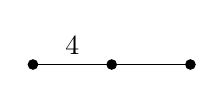
\begin{tikzpicture}[scale=1]
\node at (-0.5,0) [above]{$4$};
\draw (-1,0)--(0,0)--(1,0);
\filldraw
(-1,0) circle (.06)
(0,0) circle (.06)
(1,0) circle (.06);
\end{tikzpicture}\]
\item[(b)] If the edge $\{1,2\}$ is of order $5$, the graph is one of the following:
\[
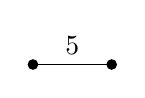
\begin{tikzpicture}[scale=1]
\node at (-0.5,0) [above]{$5$};
\draw (-1,0)--(0,0);
\filldraw
(-1,0) circle (.06)
(0,0) circle (.06);
\end{tikzpicture}\quad\quad
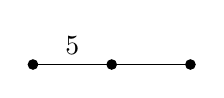
\begin{tikzpicture}[scale=1]
\node at (-0.5,0) [above]{$5$};
\draw (-1,0)--(0,0)--(1,0);
\filldraw
(-1,0) circle (.06)
(0,0) circle (.06)
(1,0) circle (.06);
\end{tikzpicture}\quad\quad
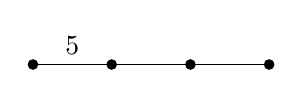
\begin{tikzpicture}[scale=1]
\node at (-0.5,0) [above]{$5$};
\draw (-1,0)--(0,0)--(1,0)--(2,0);
\filldraw
(-1,0) circle (.06)
(0,0) circle (.06)
(1,0) circle (.06)
(2,0) circle (.06);
\end{tikzpicture}\]
\end{itemize}
\end{lemma}
\begin{proof}
We can assume that $l>2$, since the lemma is trivial if $l=2$. First assume that $\{i,i+1\}$ is of order $\geq 4$ with $1\leq i\leq l-1$. Put
\[x=e_1+2e_2+\cdots+ie_i,\quad y=e_l+2e_{l-1}+\cdots+(l-i)e_{i+1}\]
and $j=l-i$. By \cref{Coxeter graph chain of order 3 prop}, we have
\[\|x\|^2=\frac{1}{2}i(i+1),\quad \|y\|^2=\frac{1}{2}j(j+1).\]
On the other hand, $(x,y)=ij(e_i,e_{i+1})=-ij\cos(\pi/m)$ with $m=4$ or $5$ (\cref{Coxeter graph oder geq 6 then 2 vertex}). Now
\[(x,y)^2\leq\|x\|^2\|y\|^2\]
which gives
\[\frac{1}{4}ij(i+1)(j+1)>i^2j^2\cos^2(\pi/m)\]
so
\[(i+1)(j+1)>4ij\cos^2(\pi/m)\geq 2ij.\]
This gives, first of all, that $ij-i-j-1<0$, or equivalently $(i-1)(j-1)<2$. If $1<i<l-1$, then $1<j<l-1$, so $i=j=2$ and
\[16\cos^2(\pi/m)<9\]
since $\cos(\pi/5)=(1+\sqrt{5})/4$, this implies $m=4$ and proves (a). If $i=1$ and $m=5$, then $2j+2>4j\cos^2(\pi/5)$, or $ j<\sqrt{5}+1<4$. This shows $l=j+1\leq 4$, and proves (b).
\end{proof}
\begin{lemma}\label{Coxeter graph ramification length of three chain classification}
If $\Gamma$ has a ramification point $i$, the full subgraph $\Gamma\setminus\{i\}$ is the union of three chains, and if $r-1,s-1,t-1$ are the lengths of these chains, the triple $\{r,s,t\}$ is equal, up to a permutation, to one of the triples $\{1,2,2\}$, $\{1,2,3\}$, $\{1,2,4\}$, $\{1,1,m\}$ (for some $m\geq 1$).
\end{lemma}
\begin{proof}
The vertex $i$ belongs to $3$ edges by \cref{Coxeter graph at most 3 edge}, and there is no other ramification point by \cref{Coxeter graph classification ramification or not}, so the full subgraph $\Gamma\setminus\{i\}$ is the sum of $3$ chains $\Gamma_1,\Gamma_2$, and $\Gamma_3$, each of which has a terminal vertex linked to $i$ in $\Gamma$. Let $\{i_1,i_2\},\dots,\{i_{r-1},i_r\}$ be the edges Of $\Gamma_2$, $\{j_1,j_2\},\dots,\{j_{s-1},j_s\}$ those of $\Gamma_2$, and $\{k_1,k_2\},\dots,\{k_{t-1},k_t\}$ those of $\Gamma_3$, with $i_1,j_1,k_1$ linked to $i$ in $\Gamma$. We can assume that $r\geq s\geq t\geq 1$. Put
\[x=e_{i_r}+2e_{i_{r-1}}+\cdots+re_{i_1},\quad y=e_{j_s}+2e_{j_{s-1}}+\cdots+se_{j_1},\quad z=e_{k_t}+2e_{k_{t-1}}+\cdots+te_{k_1}.\]
Since all the edges of $\Gamma$ are of order $3$ (\cref{Coxeter graph classification ramification or not}), \cref{Coxeter graph chain of order 3 prop} gives
\[\|x\|^2=\frac{1}{2}r(r+1),\quad \|y\|^2=\frac{1}{2}s(s+1),\quad\|z\|^2=\frac{1}{2}t(t+1).\]
On the other hand, $e_i$ is orthogonal to vectors other than $e_{i_1},e_{j_1},e_{k_1}$, so
\[(e_i,x)=-\frac{1}{2}p,\quad (e_i,y)=-\frac{1}{2}s,\quad (e_i,z)=-\frac{1}{2}t.\]
The unit vectors $\|x\|^{-1}x$, $\|y\|^{-1}y$, and $\|z\|^{-1}z$ are mutually orthogonal, and $e_i$ does not belong to the subspace $F$ they generate; the suqre of the distance from $e_i$ to $F$ is
\begin{align*}
1-(e_i,\frac{x}{\|x\|})^2-(e_i,\frac{y}{\|y\|})^2-(e_i,\frac{z}{\|z\|})^2&=1-\frac{r}{2(r+1)}-\frac{s}{2(s+1)}-\frac{t}{2(t+1)}\\
&=\frac{1}{2(r+1)}+\frac{1}{2(s+1)}+\frac{1}{2(t+1)}-\frac{1}{2}.
\end{align*}
Since this quantity is positive, we have
\begin{align}\label{Coxeter graph ramification length of three chain classification-1}
(r+1)^{-1}+(s+1)^{-1}+(t+1)^{-1}>1.
\end{align}
Hence $3(t+1)^{-1}>1$ and finally $r=1$. Then (\ref{Coxeter graph ramification length of three chain classification-1}) gives
\begin{align}\label{Coxeter graph ramification length of three chain classification-2}
(r+1)^{-1}+(s+1)^{-1}>\frac{1}{2}
\end{align}
hence $2(s+1)^{-1}>1/2$, so $s\leq 2$. Finally, if $s=2$, (\ref{Coxeter graph ramification length of three chain classification-2}) gives $(r+1)^{-1}>1/6$, hence $r\leq 4$.
\end{proof}
\begin{theorem}\label{Coxeter graph of finite irreducible classification}
The graph of any irreducible finite Coxeter system $(W,S)$ is isomorphic to one of the following:
{\renewcommand\arraystretch{1.5}
\begin{longtable}[c]{m{1cm}m{7cm}m{2cm}}
$A_l$&\begin{dynkinDiagram}[Coxeter]A{}
\end{dynkinDiagram}&($l\geq 1$)\\
$B_l$&\begin{dynkinDiagram}[Coxeter]B{}
\end{dynkinDiagram}&($l\geq 1$)\\
$D_l$&\begin{dynkinDiagram}[Coxeter]D{}
\end{dynkinDiagram}&($l\geq 4$)\\
$E_6$&\begin{dynkinDiagram}[Coxeter]E{6}
\end{dynkinDiagram}&\\
$E_7$&\begin{dynkinDiagram}[Coxeter]E{7}
\end{dynkinDiagram}&\\
$E_8$&\begin{dynkinDiagram}[Coxeter]E{8}
\end{dynkinDiagram}&\\
$F_4$&\begin{dynkinDiagram}[Coxeter]F{4}
\end{dynkinDiagram}&\\
$G_2$&\begin{dynkinDiagram}[Coxeter,gonality=6]G{2}
\end{dynkinDiagram}&\\
$H_3$&\begin{dynkinDiagram}[Coxeter]H{3}
\end{dynkinDiagram}&\\
$H_4$&\begin{dynkinDiagram}[Coxeter]H{4}
\end{dynkinDiagram}&\\
$I_2(p)$&\begin{dynkinDiagram}[Coxeter,gonality=p]I{}
\end{dynkinDiagram}&\\
\end{longtable}
}
Moreover, no two of these graphs are isomorphic.
\end{theorem}
\begin{proof}
Indeed, let $W=(m_{ij})$ be the Coxeter matrix of $(W,S)$, and let $I=|S|$. If one of the $m_{ij}$ is $\geq 6$, then $l=2$ by \cref{Coxeter graph oder geq 6 then 2 vertex} and the Coxeter graph of $(W, S)$ is of type $G_2$ or $I_2(p)$ with $p\geq 7$. Assume now that all the $m_{ij}\leq 5$.\par
If the $m_{ij}$ are not all equal to $3$, then the graph $\Gamma$ of $(W,S)$ is a chain and exactly one of the $m_{ij}$ is equal to $4$ or $5$ by \cref{Coxeter graph classification ramification or not}. If one of the $m_{ij}$ is equal to $5$, \cref{Coxeter graph chain high order 4 and 5 iff} shows that we have one of the types $H_3$, $H_4$ or $I_2(5)$. If one of the $m_{ij}$ is equal to $4$, \cref{Coxeter graph chain high order 4 and 5 iff} shows that we have one of the types $B_l$ or $F_4$.\par
Assume now that all the $m_{ij}$ are equal to $3$. If $X$ is a chain, the Coxeter graph is of type $A_l$. If not, \cref{Coxeter graph ramification length of three chain classification} shows that it is of type $E_6$, $E_7$, $E_8$ or $D_l$. The fact that no two of the Coxeter graphs listed are isomorphic is clear.
\end{proof}
\begin{theorem}\label{Coxeter graph defined by classification are finite}
The Coxeter groups defined by the Coxeter graphs of \cref{Coxeter graph of finite irreducible classification} are finite.
\end{theorem}
\begin{proof}
This is clear for $I_2(p)$, the corresponding group being the dihedral group of order $2p$. For $H_4$ the matrix $(q_{ij})$ is
\begin{align*}
Q=\begin{pmatrix}
1&-\frac{1}{2}&0&0\\
-\frac{1}{2}&1&-\frac{1}{2}&0\\
0&-\frac{1}{2}&1&-\cos\frac{\pi}{5}\\
0&0&-\cos\frac{\pi}{5}&1
\end{pmatrix}
\end{align*}
By computing the principal minors for this matrix, we see $Q$ is positive and non-degenerate, so the corresponding Coxeter group is finite. The same holds for that corresponding to $H_3$, since it is isomorphic to a subgroup of the preceding.\par
For the types $A_l,B_l,\dots,G_2$, we shall construct root systems having the corresponding groups as Weyl groups. We shall see that these groups are not only finite, but crystallographic.
\end{proof}
\subsection{Dynkin graphs}
By abuse of language, we shall call a \textbf{normed graph} a pair $(\Gamma,f)$ having the following properties:
\begin{itemize}
\item[(a)] $\Gamma$ is a graph (called the \textbf{underlying graph} of $(\Gamma,f)$).
\item[(b)] If $E$ denotes the set of pairs $(i,j)$ such that $\{i,j\}$ is an edge of $\Gamma$, $f$ is a map from $E$ to $\R$ such that $f(i,j)f(j,i)=1$ for all $(i,j)\in E$.
\end{itemize}
There is an obvious notion of isomorphism of normed graphs.\par
Let $\Phi$ be a reduced root system in a real vector space $V$. We are going to associate to it a normed graph $(\Gamma,f)$, called the Dynkln graph of $\Phi$. The vertices of $\Gamma$ will be the elements of the set $I$ of orbits of $W(\Phi)$ in the union of the sets $\{\Delta\}\times\Delta$ (where $\Delta$ is a basis of $\Phi$). If $N=(n_{ij})_{i,j\in I}$ (resp. $M=(m_{ij})_{i,j\in I}$ is the canonical Cartan matrix (resp. the Coxeter matrix) of $\Phi$, two vertices $i$ and $j$ of $\Gamma$ are linked if and only if $n_{ij}\neq 0$ and we then put
\[f(i,j)=\frac{n_{ij}}{n_{ji}}.\]
Since $n_{ij}=0$ implies $n_{ji}=0$, this defines a normed graph $(\Gamma,f)$.\par
Let $(\cdot\,,\cdot)$ be a scalar product on $V$, invariant under $W(\Phi)$, and let $\Delta=(\alpha_i)_{i\in I}$ be a basis of $\Phi$, indexed canonically. Then that vertices $i$ and $j$ of the graph $\Gamma$ are linked if and only if $(\alpha,\alpha_j)\neq 0$, and
\[f(i,j)=\frac{n(\alpha_i,\alpha_j)}{n(\alpha_j,\alpha_i)}=\frac{(\alpha_i,\alpha_i)}{(\alpha_j,\alpha_j)}.\]
In view of Table~\ref{root system angle case}, the only possibilities are the following, up to interchanging $i$ and $j$:
\begin{itemize}
\item[(1)] $i$ and $j$ are not linked, and $n_{ij}=n_{ji}=0$, $m_{ij}=2$;
\item[(2)] $f(i,j)=f(j,i)=1$ and $n_{ij}=n_{ji}=-1$, $m_{ij}=3$;
\item[(3)] $f(i,j)=2$, $f(j,i)=1/2$, and $n_{ij}=n_{ji}=-2$, $m_{ij}=4$;
\item[(4)] $f(i,j)=3$, $f(j,i)=1/3$, and $n_{ij}=n_{ji}=-3$, $m_{ij}=6$;
\end{itemize}
We see from this that the Dynkin graph $\Phi$ determines the Cartan matrix and the Coxeter matrix of $\Phi$, and hence determines $\Phi$ up to isomorphism. More precisely, Corollary~\ref{root system bijection on base induce iso} implies the following result:
\begin{proposition}\label{Dynkin graph iso induce root system iso}
Let $\Phi_1$ and $\Phi_2$ be two reduced root systems in vector spaces $V_1$ and $V_2$. Let $\Delta_1=(\alpha_i)_{i\in I_1}$ and $\Delta_2=(\alpha_i)_{i\in I_2}$ be bases of $\Delta_1$ and $\Delta_2$, indexed canonically. Let $\theta$ be an isomorphism from the Dynkin graph of $\Phi_1$ to the Dynkin graph of $\Phi_2$. Then, there exists a unique isomorphism from $V_1$ to $V_2$ transforming $\Phi_1$ into $\Phi_2$ and $\alpha_i$ into $\alpha_{\theta(i)}$ for all $i\in I_1$.
\end{proposition}
It is clear that an automorphism of $\Phi$ defines an automorphism of the Dynkin graph of $\Phi$, and hence a homomorphism $\Pi$ from the group $\Aut(\Phi)$ to the group of automorphisms of the Dynkin graph of $\Phi$.
\begin{corollary}\label{Dynkin graph automorphism is Aut/W}
The homomorphism $\Pi$ defines by passage to the quotient an isomorphism from the group $\Aut(\Phi)/W(\Phi)$ to the group of automorphisms of the Dynkin graph of $\Phi$.
\end{corollary}
\begin{proof}
Recall that an vertex $i$ represents an orbit of $W$ in the union of the sets $\{\Delta\}\times\Delta$, where $\Delta$ is a basis. Therefore $\Pi(w)=1$ for all $w\in W(\Phi)$. On the other hand, \cref{Dynkin graph iso induce root system iso} shows that there exists an isomorphism $\Xi$ from the group of isomorphisms of the Dynkin graph of $\Phi$ to the subgroup $G$ of elements of $\Aut(\Phi)$ leaving fixed a given basis $\Delta$ of $\Phi$, such that $\Pi\circ\Xi=1$. Since $\Aut(\Phi)$ is the semi-direct product of $G$ and $W(\Phi)$, the corollary follows.
\end{proof}
In practice, the Dynkin graph $(\Gamma,f)$ is represented by a diagram composed of nodes and bonds in the following way. The nodes correspond to the vertices of $\Gamma$; two nodes corresponding to two distinct vertices $i$ and $j$ are joined by $0$, $1$, $2$ or $3$ bonds in cases (1), (2), (3) and (4) above (up to interchanging $i$ and $j$). Moreover, in cases (3) and (4), that is when $f(i,j)>1$, or when the roots $\alpha_i$ and $\alpha_j$ are not orthogonal and not of the same length, an inequality sign $>$ is placed on the double or triple bond joining the nodes corresponding to $i$ and $j$ oriented towards the node corresponding to $j$ (that is, the shortest root):
\[
\dynkin[]{B}{2}\text{\hspace{5pt} if $f(i,j)=2$}\quad\quad\quad \dynkin[style,]{G}{2}\text{\hspace{5pt} if $f(i,j)=3$}.\]
It is clear that the Dynkin graph $(\Gamma,f)$ can be recovered from this diagram.\par
We remark that the diagram associated to the Coxeter graph of $W(\Phi)$ can be obtained from that associated to the Dynkin graph of $\Phi$ by keeping the nodes and the single bonds and replacing the double (resp. triple) bonds by a bond surmounted by the number $4$ (resp. $6$). Conversely, given the Coxeter graph of $W(\Phi)$, the diagram associated to the Dynkin graph of $\Phi$ can be recovered using the inverse of this procedure, except for the inequality signs on the double or triple bonds. \cref{Coxeter graph of finite irreducible classification} thus gives immediately the list of possible Dynkin graphs. More precisely:
\begin{theorem}\label{Dynkin graph finite classification}
If $\Phi$ is an irreducible reduced root system, its Dynkin graph is isomorphic to one of the graphs represented by the following diagrams:
{\renewcommand\arraystretch{1.5}
\begin{longtable}[c]{m{1cm}m{7cm}m{2cm}}
$A_l$&\begin{dynkinDiagram}A{}
\end{dynkinDiagram}&($l\geq 1$)\\
$B_l$&\begin{dynkinDiagram}B{}
\end{dynkinDiagram}&($l\geq 2$)\\
$C_l$&\begin{dynkinDiagram}C{}
\end{dynkinDiagram}&($l\geq 3$)\\
$D_l$&\begin{dynkinDiagram}D{}
\end{dynkinDiagram}&($l\geq 4$)\\
$E_6$&\begin{dynkinDiagram}E{6}
\end{dynkinDiagram}&\\
$E_7$&\begin{dynkinDiagram}E{7}
\end{dynkinDiagram}&\\
$E_8$&\begin{dynkinDiagram}E{8}
\end{dynkinDiagram}&\\
$F_4$&\begin{dynkinDiagram}F{4}
\end{dynkinDiagram}&\\
$G_2$&\begin{dynkinDiagram}G{2}
\end{dynkinDiagram}&\\
\end{longtable}
}
Moreover, no two of these graphs are isomorphic and there are irreducible reduced root systems having each of them as their Dynkin graph (up to isomorphism).
\end{theorem}
\begin{proof}
The first assertion follows immediately from \cref{Coxeter graph of finite irreducible classification}, in view of the preceding remarks, the fact that the Coxeter groups of the graphs $H_3$, $H_4$ and $I_2(p)$ (for $p=5$ and $p\geq 7$) are not crystallographic, and the fact that the two possible inequalities for the double (resp. triple) bond of the Dynkin graph associated to the Coxeter graph $F_4$ (resp. $G_2$) give isomorphic Dynkin graphs. The second assertion is clear and the third will follow from the explicit construction of an irreducible reduced root system for each type.
\end{proof}
\begin{remark}
The graph $A_1$ reduces to a single node; we denote it also by $B_1$ or $C_1$. The graph $B_2$ is also denoted by $C_2$, since they are isomorphic. The graph $A_3$ is also denoted by $D_3$. Finally, $D_2$ denotes the graph consisting of two unconnected nodes. (These conventions are derived from the properties of the corresponding root systems)
\end{remark}
\begin{remark}
If $(\Gamma,f)$ is the Dynkin graph of a reduced root system $\Phi$, the Dynkin graph of the inverse system can be identified with $(\Gamma,f^{-1})$. In other words, the diagram associated to the Dynkin graph of $\check{\Phi}$ can be obtained from that associated to the Dynkin graph of $\Phi$ by reversing the inequality signs. If $\Phi$ is irreducible, we see that $\Phi$ is isomorphic to $\check{\Phi}$ unless $\Phi$ is of type $B_l$ or $C_l$, in which case $\check{\Phi}$ is of type $C_l$ or $B_l$.
\end{remark}
\begin{example}[\textbf{Automorphism groups for connected Dynkin graphs}]
As an application of \cref{Dynkin graph finite classification}, we compute the automorphim of all connected Dynkin diagrams, so that by Corollary~\ref{Dynkin graph automorphism is Aut/W} we can determine the automorphim of reduced irreducible root systems. Let $\Gamma$ be one of the graphs in \cref{Dynkin graph finite classification}. First we note that, if $\Gamma$ is not simply-laced (which means it has $>$ in it), then the automorphim group of $\Gamma$ is trivial. In fact, in this case any automorphim $\tau$ of $\Gamma$ must preserve the edge $\{i,j\}$ such that $n(i,j)\neq 1$ and therefore fixes $i$ and $j$. With this, since we see in any case the vertex $i$ or $j$ is linked to another unique vertex $k$, this vertex is also fixed by $\tau$. Continuing this argument, we see that $\tau$ eventually fixes all vertices of $\Gamma$, so $\tau=1$. Comparing with \cref{Dynkin graph finite classification}, we get
\[\Aut(B_l)=\Aut(C_l)=\Aut(F_4)=\Aut(G_2)=\{1\}.\]
As an example, we compute the automorphims of the Dynkin graph $A_l$, which is given by
\[\dynkin[labels={1,2,l-1,l}]A{}\]
Let $\tau\in\Aut(A_l)$. Then $\tau$ sends terminal vertices to terminal vertices, so $\tau(1)=1$ or $\tau(1)=l$. From this and the fact that $\tau$ send edges to edges, we conclude that $\tau(i)=i$ or $\tau(i)=l+1-i$ for all $i$. If we denote the second automorphim by $-1$, then $\Aut(A_l)=\{1,-1\}\cong\Z/2\Z$.\par
Following this partten, one easily computes the automorphim groups for the rest simply-laced Dynkin graphs. We list our result in the following table:
{\renewcommand\arraystretch{1.5}
\begin{longtable}[c]{m{1cm}m{7cm}m{5cm}}
$A_l$&\begin{dynkinDiagram}A{}
\end{dynkinDiagram}&$\Aut(A_l)=\Z/2\Z$\\
$B_l$&\begin{dynkinDiagram}B{}
\end{dynkinDiagram}&$\Aut(B_l)=\{1\}$\\
$C_l$&\begin{dynkinDiagram}C{}
\end{dynkinDiagram}&$\Aut(C_l)=\{1\}$\\
$D_4$&\begin{dynkinDiagram}D{4}
\end{dynkinDiagram}&$\Aut(D_4)=\mathfrak{S}_3$\\
$D_l$&\begin{dynkinDiagram}D{}
\end{dynkinDiagram}&$\Aut(D_l)=\Z/2\Z\quad\text{($l>4$)}$\\
$E_6$&\begin{dynkinDiagram}E{6}
\end{dynkinDiagram}&$\Aut(E_6)=\Z/2\Z$\\
$E_7$&\begin{dynkinDiagram}E{7}
\end{dynkinDiagram}&$\Aut(E_7)=\{1\}$\\
$E_8$&\begin{dynkinDiagram}E{8}
\end{dynkinDiagram}&$\Aut(E_8)=\{1\}$\\
$F_4$&\begin{dynkinDiagram}F{4}
\end{dynkinDiagram}&$\Aut(F_4)=\{1\}$\\
$G_2$&\begin{dynkinDiagram}G{2}
\end{dynkinDiagram}&$\Aut(G_2)=\{1\}$\\
\end{longtable}
}
\end{example}
Let $\Phi$ be an irreducible reduced root system and $(\Gamma,f)$ be its Dynkin graph. We are going to define another normed graph $(\tilde{\Gamma},\tilde{f})$ that we shall call the \textbf{completed Dynkin graph} of $\Phi$. The set $\tilde{I}$ of vertices of $\Gamma$ consists of the set $I$ of vertices of $\Gamma$ and a vertex denoted by $0$, not belonging to $I$. To define $\tilde{f}$, choose a basis $\Delta=(\alpha_i)_{i\in I}$ of $\Phi$ and a scalar product $(\cdot\,,\cdot)$ invariant under $W(\Phi)$. Let $\alpha_0=-\tilde{\alpha}$ be the negative of the highest root $\tilde{\alpha}$ for the order defined by $\Delta$. Two distinct vertices $i,j\in I$ are linked if and only if $(\alpha_i,\alpha_j)\neq 0$ and we then put
\[\tilde{f}=\frac{(\alpha_i,\alpha_i)}{(\alpha_j,\alpha_j)}.\]
It is immediate that the graph $\tilde{\Gamma}$ and the map $\tilde{f}$ thus defined do not depend on the choice of $\Delta$ or the scalar product.\par
If the rank $l$ of $\Phi$ is equal to $1$, then $I=\{i\}$ and $\alpha_0=-\alpha_1$; hence $\tilde{f}(0,i)=1$. If $l\geq 2$, $\alpha_0$ is not proportional to any of the $\alpha_i$ and $(\alpha_0,\alpha_i)$ is negative (\cref{root system highest root}). For any pair $(i,j)$ of distinct elements of $I$, the only possibilities are those mentioned above (putting, for example, $n_{0i}=n(\alpha_0,\alpha_i)$ and $m_{0,i}$ be order of $s_{\alpha_0}s_{\alpha_i}$ for all $i\in I$).\par
In the case $l\geq 2$, the completed Dynkin graph is represented by a diagram with the same conventions as before, sometimes indicating by dotted lines the bonds joining the vertex $0$ to the other vertices. We remark that the inequality sign $>$ on such a bond, if it exists, is always directed towards the vertex distinct from $0$, since $\alpha_0$ is a longest root (\cref{root system highest root}). The graph $(\Gamma,f)$ is the subgraph obtained from $(\tilde{\Gamma},\tilde{f})$ by deleting the vertex $0$. The action of $\Aut(\Phi)$ on $(\Gamma,f)$ extends to an action on $(\tilde{\Gamma},\tilde{f})$, leaving $0$ fixed, and $W(\Phi)$ acts trivially on $(\tilde{\Gamma},\tilde{f})$. Let $W_a(\Phi)$ be the affine Weyl group of $\Phi$. Then \cref{root system alcove char} together with \cref{reflection group is Coxeter system} shows that the Coxeter graph $\Sigma$ of the affine Weyl group $W_a(\Phi)$ can be obtained from $(\Gamma,f)$, and the index set $\tilde{
I}$ can be viewed as the set of orbits of $W_a(\Phi)$ in the union of sets $\{\Delta\cup\{\tilde{\alpha}\}\}\times(\Delta\cup\{\tilde{\alpha}\})$.\par
On the other hand, let $N$ be the normaliser of $W_a(\Phi)$. To any $g\in N$ corresponds an automorphism $\Pi(g)$ of $\Sigma$ and $\Pi(g)=1$ if $g\in W_a(\Phi)$. Conversely, given an automorphism $\theta$ of $\Sigma$ there is, by \cref{Coxeter group infinite positive degenerate form}, a unique element $g=\Xi(\theta)$ preserving a given alcove $A$ and such that $\Pi(g)=\theta$. Since $N$ is the semi-direct product of the subgroup $N_A$ of elements preserving $A$ and $W_a(\Phi)$, we deduce that $\Pi$ defines by passage to the quotient an isomorphism from $N/W_a(\Phi)=N_A$ to $\Aut(\Sigma)$. Recall that the group $N/W_a(\Phi)$ can be identified with the semi-direct product of $\Aut(\Phi)/W(\Phi)$ and $\Lambda(\check{\Phi})/\Lambda_r(\check{\Phi})$, therefore the group $\Aut(\Sigma)$ is also isomorphic to this semi-direct product. We also recall that the group $\Lambda(\check{\Phi})/\Lambda_r(\check{\Phi})$ is isomorphic to the group $\Gamma_A=N_A\cap\widehat{W}_a(\Phi)$, and that the elements $\gamma_i$ in \cref{root system Gamma_A bijection} correspond to nontrivial representatives in $\Lambda(\check{\Phi})/\Lambda_r(\check{\Phi})$. The element of $\Aut(\Sigma)$ corresponding to the element $\gamma_i$ of $\Gamma_A$ transforms the vertex $0$ to the vertex $i$ of $\Sigma$, in view of \cref{root system alcove gamma_A conjugate action prop}.
\begin{theorem}
Let $(W,S)$ be an irreducible Coxster system with $S$ finite. Then the associated quadratic form is positive and degenerate if and only if the Coxeter graph of $(W,S)$ is isomorphic to one of the following:
{\renewcommand\arraystretch{1.5}
\begin{longtable}[c]{m{0.7cm}m{1.5cm}m{7.5cm}}
$\widetilde{A}_1$&&\begin{dynkinDiagram}[extended,Coxeter]A{1}
\end{dynkinDiagram}
\\
$\widetilde{A}_l$&($l\geq 2$)&\begin{dynkinDiagram}[extended,Coxeter]A{}
\end{dynkinDiagram}\\
$\widetilde{B}_2$&&\begin{dynkinDiagram}[extended,Coxeter]B{2}
\end{dynkinDiagram}
\\
$\widetilde{B}_l$&($l\geq 3$)&\begin{dynkinDiagram}[extended,Coxeter]B{}
\end{dynkinDiagram}\\
$\widetilde{C}_l$&($l\geq 3$)&\begin{dynkinDiagram}[extended,Coxeter]C{}
\end{dynkinDiagram}\\
$\widetilde{D}_l$&($l\geq 4$)&\begin{dynkinDiagram}[extended,Coxeter]D{}
\end{dynkinDiagram}\\
$\widetilde{E}_6$&&\begin{dynkinDiagram}[extended,Coxeter]E{6}
\end{dynkinDiagram}\\
$\widetilde{E}_7$&&\begin{dynkinDiagram}[extended,Coxeter]E{7}
\end{dynkinDiagram}\\
$\widetilde{E}_8$&&\begin{dynkinDiagram}[extended,Coxeter]E{8}
\end{dynkinDiagram}\\
$\widetilde{F}_4$&&\begin{dynkinDiagram}[extended,Coxeter]F{4}
\end{dynkinDiagram}\\
$\widetilde{G}_2$&&\begin{dynkinDiagram}[extended,Coxeter]G{2}
\end{dynkinDiagram}\\
\end{longtable}
}
Moreover, no two of these Coxeter graphs are isomorphic.
\end{theorem}
\begin{proof}
By \cref{Coxeter group infinite positive degenerate form}, the Coxeter systems whose quadratic form is positive and degenerate are those which correspond to the affine Weyl groups of irreducible reduced root systems. The theorem therefore follows from the determination of the completed Dynkin graphs.
\end{proof}
\chapter{Semi-simple Lie algebras and its representations}
In this section, $\K$ denotes a field. By a vector space, we mean a vector space over $\K$, and similarly for "Lie algebra", etc. All Lie algebras are assumed to be finite dimensional.
\section{Cartan subalgebras and regular elements}\label{Lie algebra Cartan subalgebra section}
\subsection{Root decomposition of representations}
Let $V$ be a vector space and $S$ a set. A \textbf{representation} of $S$ on $V$ is defined to be a map $\rho:S\to\End(V)$. Let $\mathcal{P}(S)$ (or $\mathcal{P}$ if the set $S$ is understood) denote the set of all maps from $S$ to $\K$. For any $\lambda\in\mathcal{P}$, we denote by $V_\lambda(S)$ (resp. $V^\lambda(S)$) the subspaces of $V$ defined by
\begin{align*}
V_\lambda(S)=\{v\in V:\text{$\rho(s)\cdot v=\lambda(s)v$ for all $s\in S$}\}
\end{align*}
and
\begin{align*}
V^\lambda(S)=\{v\in V:\text{$(\rho(s)-\lambda(s))^nv=0$ for $n$ sufficiently large}\}.
\end{align*}
We say that $V_\lambda(S)$ is the \textbf{eigenspace} of $V$ relative to $\lambda$ (and to $\rho$), that $V^\lambda(S)$ is the \textbf{primary subspace} of $V$ relative to $\lambda$ (and to $\rho$). Also, the space $V_0(S)$ is called that \textbf{nilspace} of $V$ (relative to $\rho$). We say $\lambda$ is a \textbf{weight} of $S$ in $V$ if $V^\lambda(S)\neq 0$, and the set of all weights of $V$ is denoted by $\mathcal{P}(V)$.\par
In particular, if $S$ reduces to a single element $s$, then the set $\mathcal{P}$ can be identified with $\K$, and we may use the notations $V_\lambda(s)$ and $V^\lambda(s)$ instead of $V_\lambda(\{s\})$ and $V^\lambda(\{s\})$. We speak of eigenspaces, primary subspaces and the nilspace of $\rho(s)$; an element $v$ of $V_\lambda(s)$ is called an \textbf{eigenvector} of $\rho(s)$, and $v\neq 0$, $\lambda(s)$ is called the corresponding \textbf{eigenvalue} of $\rho(s)$. For any map $\lambda:S\to \K$, the following relations are immediate:
\[V_\lambda(S)=\bigcap_{s\in S}V_\lambda(s),\quad V^\lambda(S)=\bigcap_{s\in S}V^\lambda(S).\]

Let $\K'$ be an extension of $\K$. The canonical map from $\End(V)$ to $\End(V\otimes_\K\K')$ gives, by composition with $\rho$, a map $\tilde{\rho}:S\to\End(V\otimes_\K\K')$. Similarly, every map $\lambda:S\to \K$ can be viewed as a map from $S$ to $\K'$. With these notations, we have the following proposition:
\begin{proposition}\label{set rep eigenspace under field extension}
For any map $\lambda\in\mathcal{P}$, we have
\[(V\otimes_\K\K')_\lambda(S)=V_\lambda(S)\otimes_\K\K',\quad(V\otimes_\K\K')_\lambda(S)=V_\lambda(S)\otimes_\K\K'\]
\end{proposition}
\begin{proof}
Let $(\alpha_i)$ be a basis of the $\K$-vector space $\K'$. If $v\in V\otimes_\K\K'$, then $v$ can be expressed uniquely in the form $\sum_iv_i\otimes\alpha_i$ where $(v_i)$ is a finitely-supported family of elements of $V$. For all $s\in S$ and $n\in\N$,
\[(\tilde{\rho}(s)-\lambda(s))^nv=\sum(\rho(s)-\lambda(s))^nv_i\otimes\alpha_i\]
from which the claim follows.
\end{proof}
For two representations $(V,\rho)$ and $(W,\eta)$ of $S$, we define an \textbf{$\bm{S}$-homomorphism} to be a linear map $\varphi:V\to W$ such that for each $s\in S$ and $v\in V$ we have
\[\varphi(\rho(s)v)=\eta(s)\varphi(v).\]
We say the $S$-homomorphism $\varphi$ is injective, surjective, or bijective if the map $\varphi$ is injective, surjective, bijective respectively.
\begin{proposition}\label{set rep eigenspace under homomorphism}
Let $(U,\theta)$, $(V,\rho)$, and $(W,\eta)$ be representations of $S$.
\begin{itemize}
\item[(a)] Let $\varphi:V\to W$ be an $S$-homomorphism. Then $\varphi$ maps $V_\lambda(S)$ (resp. $V^\lambda(S)$) into $W_\lambda(S)$ (resp. $W^\lambda(S)$) for any $\lambda\in\mathcal{P}$.
\item[(b)] Let $B:V\times W\to U$ be a bilinear map such that
\[\theta(s)B(v,w)=B(\rho(s)v,w)+B(v,\eta(s)w)\]
for $s\in S$ and $v\in V$, $w\in W$. Then for any $\lambda,\mu\in \mathcal{P}$, $B$ maps $V_\lambda(S)\times W_\mu(S)$ (resp. $V^\lambda(S)\times W^\mu(S)$) into $U_{\lambda+\mu}(S)$ (resp. $U^{\lambda+\mu}(S)$). 
\item[(c)] Let $B:V\times W\to U$ be a bilinear map such that
\[\theta(s)B(v,w)=B(\rho(s)v,\eta(s)w)\]
for $s\in S$ and $v\in V$, $w\in W$. Then for any $\lambda,\mu\in \mathcal{P}$, $B$ maps $V_\lambda(S)\times W_\mu(S)$ (resp. $V^\lambda(S)\times W^\mu(S)$) into $U_{\lambda\mu}(S)$ (resp. $U^{\lambda\mu}(S)$). 
\end{itemize}
\end{proposition}
\begin{proof}
In case (a), for any $s\in S$ and $v\in V$ we have
\[(\eta(s)-\lambda(s))^n\varphi(v)=\varphi((\rho(s)-\lambda(s))^nv)\]
hence the conclusion. In case (b), for any $s\in S$ and $v\in V$,
\[(\theta(s)-\lambda(s)-\mu(s))B(v,w)=B((\rho(s)-\lambda(s))v,w)+B(v,(\eta(s)-\mu(s))w)\]
hence by induction on $n$ we get
\[(\theta(s)-\lambda(s)-\mu(s))B(v,w)=\sum_{i+j=n}\binom{n}{i}B((\rho(s)-\lambda(s))^iv,w)+B(v,(\eta(s)-\mu(s))^jw).\]
The assertions in (b) follow immediately. In case (c), however, we have
\[(\theta(s)-\lambda(s)\mu(s))B(v,w)=B((\rho(s)-\lambda(s))v,\eta(s)w)+B(\lambda(s)v,(\eta(s)-\mu(s))w)\]
for $s\in S$, $v\in V$, $w\in W$. Again by induction on $n$, we find
\[(\theta(s)-\lambda(s)\mu(s))^nB(v,w)=\sum_{i+j=n}\binom{n}{i}B(\lambda(s)^{j}(\rho(s)-\lambda(s))^iv,\eta(s)^i(\eta(s)-\mu(s))^jw).\]
The assertions in (c) follow immediately.
\end{proof}
\begin{proposition}\label{set rep eigenspace direct sum}
The sums $\sum_{\lambda\in \mathcal{P}}V_\lambda(S)$ and $\sum_{\lambda\in \mathcal{P}}V^\lambda(S)$ are direct.
\end{proposition}
\begin{proof}
Since $V_\lambda(S)\sub V^\lambda(S)$, we only need to prove $\sum_{\lambda\in \mathcal{P}}V^\lambda(S)$ is direct. For this, we will show that any linera combination of weight vectors can not be a weight vector again unless it is zero.\par
If $S$ is empty, the claim is trivial. If $S$ is reduced to a single element $s$, let $\lambda_0,\lambda_1,\dots,\lambda_n$ be distinct elements of $\K$. For each $i=0,\dots,n$ let $v_i\in V^{\lambda_i}(s)$ and assume that $v_0=a_1v_1+\cdots+a_nv_n$. It suffices to prove that $v_0=0$. For each $i$, there exists an integer $r_i>0$ such that $(\rho(s)-\lambda_i)^{r_i}(v_i)=0$.  Consider the polynomials
\[P(T)=\prod_{i=1}^{n}(T-\lambda_i)^{r_i},\quad Q(T)=(T-\lambda_0)^{r_0}.\]
We then have
\[Q(\rho(s))v_0=0,\quad P(\rho(s))v_0=\sum_{i=1}^{n}a_iP(\rho(s))v_i=0.\]
Since $P$ and $Q$ are relatively prime, the Bezout identity proves that $v_0=0$.\par
Now we assume that $S$ is finite and prove the claim by induction on the cardinality of $S$. Let $s\in S$ and $\widetilde{S}=S\setminus\{s\}$. Let $(v_\lambda)_{\lambda\in \mathcal{P}}$ be a finitely-supported family of elements of $V$ and $(a_\lambda)$ a finitely-supported family of elements of $\K$ such that
\begin{align}\label{set rep eigenspace disjoint-1}
v_{\lambda_0}=\sum_{\lambda\in \mathcal{P}}a_\lambda v_\lambda\in V^{\lambda_0}(S),\quad v_\lambda\in V^\lambda(S),
\end{align}
where $\lambda_0\in\mathcal{P}$. Let $\tilde{\mathcal{P}}$ be the set of $\lambda\in\mathcal{P}$ such that $\lambda|_{\widetilde{S}}=\lambda_0|_{\widetilde{S}}$. Then for any $\lambda\in\widetilde{S}$ we have $V^\lambda(\widetilde{S})=V^{\lambda_0}(\widetilde{S})$, so by restricting $(\ref{set rep eigenspace disjoint-1})$ on $\widetilde{S}$ we get
\[\sum_{\lambda\in \mathcal{P}\setminus\tilde{\mathcal{P}}}a_\lambda v_\lambda\in V^{\lambda_0}(\widetilde{S}),\quad v_\lambda\in V^\lambda(\widetilde{S}).\]
By the induction hypothesis applied to $\widetilde{S}$, we have $\sum_{\lambda\in\mathcal{P}\setminus\tilde{\mathcal{P}}}a_\lambda v_\lambda=0$, so equation $(\ref{set rep eigenspace disjoint-1})$ reduces to
\begin{align}\label{set rep eigenspace disjoint-2}
v_{\lambda_0}=\sum_{\lambda\in\tilde{\mathcal{P}}}a_\lambda v_\lambda,\quad v_\lambda\in V^\lambda(s).
\end{align}
If $\lambda,\mu$ are distinct elements of $\tilde{\mathcal{P}}$, then $\lambda(s)\neq\mu(s)$. Since the sum $\sum_{\lambda\in s}V^\alpha(s)$ is direct, from $(\ref{set rep eigenspace disjoint-2})$ we see $v_{\lambda_0}=0$, so the claim is proved in this case.\par
In the general case, let $(v_\lambda)_{\lambda\in \mathcal{P}}$ and $(a_\lambda)_{\lambda\in \mathcal{P}}$ be finitely-supported families of elements of $V$ and $\K$, respectively, such that
\[v_{\lambda_0}=\sum_{\lambda\in \mathcal{P}}a_\lambda v_\lambda\in V^{\lambda_0}(S),\quad v_\lambda\in V^\lambda(S).\]
Let $\tilde{\mathcal{P}}$ be the finite set of $\lambda\in \mathcal{P}$ such that $v_\lambda\neq 0$, and let $\widetilde{S}$ be a finite subset of $S$ such that the conditions $\lambda,\mu\in\tilde{\mathcal{P}}$ and $\lambda|_{\widetilde{S}}=\mu|_{\widetilde{S}}$ imply that $\lambda=\mu$. We have $v_\lambda\in V^{\lambda}(\widetilde{S})$, so applying the preceding arguments we see $v_\lambda=0$ for $\lambda\in\tilde{\mathcal{P}}$, which completes the proof.
\end{proof}
Since the sum $\sum_{\lambda\in\mathcal{P}}V^\lambda(S)$ is direct, we may seek that if there is any chance that $V=\bigoplus_{\lambda\in\mathcal{P}}V^\lambda(S)$, so that we have a nice discription of the action of $S$ on $V$. First,ecall that, if $x\in\End(V)$, we denote by $\ad(x)$ the map $y\mapsto xy-yx=[x,y]$ from $\End(V)$ to itself. 
\begin{lemma}\label{endomorphism ad nilpotent iff eigenspace invariant}
Let $V$ be a vector space and $x,y\in\End(V)$.
\begin{itemize}
\item[(a)] Assume that $V$ is finite dimensional. Then $x$ is triangularizable if and only if we have
\[V=\bigoplus_{\lambda\in \K}V^\alpha(x).\]
\item[(b)] If there exists an integer $n$ such that $\ad(x)^n(y)=0$, each $V^\alpha(x)$ is stable under $y$.
\item[(c)] Assume that $V$ is finite dimensional. If $V=\bigoplus_{\alpha\in \K}V^\alpha(x)$ and each $V^\alpha(x)$ is stable under $y$, then there exists an integer $n$ such that $\ad(x)^n(y)=0$.
\end{itemize}
\end{lemma}
\begin{proof}
Let $E=\End(V)$ and $B$ be the bilinear map defined by
\[B:E\times V\to V,\quad (x,v)\mapsto x(v).\]
By the definition of $\ad(x)$, for $x,y\in E$ and $v\in V$ we have
\[x(B(y,v))=xy(v)=yx(v)+[x,y](v)=B(y,x(v))+B([x,y],v).\]
Let $x$ operate on $E$ via $\ad(x)$, then by \cref{set rep eigenspace under homomorphism} we have $B(E^0(x),V^\alpha(x))\sub V^\alpha(x)$ for all $\alpha\in \K$. If $\ad(x)^n(y)=0$, then $y\in E^0(x)$, so that $y(V^\alpha(x))\sub V^\alpha(x)$, which proves (b).\par
To prove (c), we first note that since each $V^\alpha(x)$ is stable under $y$, we can replace $V$ by $V^\alpha(x)$ and $x$ (resp. $y$) by its restriction to $V^\alpha(x)$. Replacing $x$ by $x-\alpha$, we can assume that $x$ is nilpotent. Then, writting $\ad(x)$ as $L_x-R_x$, where $L_x$ is the left multiplication by $x$ and $R_x$ the right multiplication by $x$, we have
\begin{align}\label{endomorphism ad nilpotent iff eigenspace invariant-1}
\ad(x)^n=(L_x-R_x)^n=\sum_{i+j=n}(-1)^i\binom{n}{i}L_x^iR_x^j.
\end{align}
Since $x$ is nilpotent we see $L_x$ and $R_x$ are both nilpotent, so the claim in (c) follows from $(\ref{endomorphism ad nilpotent iff eigenspace invariant-1})$.
\end{proof}
\begin{corollary}
If $V$ is a finite dimensional vector space and there exists an integer $n$ such that $\ad(x)^n(y)=0$, then $\ad(x)^{2\dim(V)-1}(y)=0$.
\end{corollary}
\begin{proof}
This follows from $(\ref{endomorphism ad nilpotent iff eigenspace invariant-1})$ adn the fact that if $x$ is nilpotent, then $x^{\dim(V)}=0$.
\end{proof}
In the sequel, we shall say that a map $\rho:S\to\End(V)$ is \textbf{almost commutative} if for every pair $(s,t)$ of elements of $S$, there exists an integer $n$ such that
\[\ad(\rho(s))^n(\rho(t))=0.\]
An $S$-representation $(V,\rho)$ is called \textbf{almost commutative} if the map $\rho$ is almost commutative.
\begin{theorem}\label{set rep AC iff eigenspace decomposition}
Let $(V,\rho)$ be a finite dimensional $S$-representation. Then the following conditions are equivalent:
\begin{itemize}
\item[(\rmnum{1})] The map $\rho$ is almost commutative and for each $s\in S$ the endomorphism $\rho(s)$ is triangularizable.
\item[(\rmnum{2})] For all $\lambda\in \mathcal{P}$, $V^\lambda(S)$ is stable under $\rho(S)$, and $V=\bigoplus_{\lambda\in \mathcal{P}}V^\lambda(S)$.
\end{itemize}
\end{theorem}
\begin{proof}
If $V=\bigoplus_{\lambda\in\mathcal{P}}V^\lambda(S)$, then for each $s\in S$ we have $V=\bigoplus_{\lambda\in\mathcal{P}}V^\lambda(s)$, so it follows from \cref{endomorphism ad nilpotent iff eigenspace invariant} that (\rmnum{2}) implies (\rmnum{1}). Conversely, assume that condition (\rmnum{1}) is satisfied. Then \cref{endomorphism ad nilpotent iff eigenspace invariant} imply that each $V^\lambda(S)$ is stable under $\rho(S)$. It remains to prove that $V=\bigoplus_{\lambda\in\mathcal{P}}V^\lambda(S)$. We argue by induction on $\dim(V)$. We distinguish two cases.\par
If for all $s\in S$, $\rho(s)$ has a single eigenvalue $\lambda(s)$, then $V=V^\lambda(S)$, so the claim is true. On the other hand, if there exists $s\in S$ such that $\rho(s)$ has at least two distinct eigenvalues, then $V$ is the direct sum of the $V^\alpha(s)$ for $\alpha\in \K$, and $\dim(V^\alpha(s))<\dim(V)$ for all $\alpha$. Since each $V^\alpha(s)$ is stable under $\rho(S)$, it suffices to apply the induction hypothesis to complete the proof.
\end{proof}
\begin{corollary}\label{set rep eigenspace decomposition extension of scalar}
Let $(V,\rho)$ be a finite dimensional almost commutative representation of $S$. Let $\K'$ be an extension of $\K$. Assume that, for all $s\in S$, the endomorphism $\rho(s)\otimes 1$ of $V\otimes_\K\K'$ is triangularizable. Then
\[V\otimes_\K\K'=\bigoplus_{\lambda\in\mathcal{P}}(V\otimes_\K\K')^\lambda(S).\]
\end{corollary}
\begin{proof}
Let $\tilde{\rho}:S\to\End(V\otimes_\K\K')$ be the map induced by $\rho$. If $s_1,s_2\in S$, then there exists an integer $n$ such that $\ad(\rho(s_1))^n(\rho(s_2))=0$, hence $\ad(\tilde{\rho}(s_1))^n(\tilde{\rho}(s_2))=0$. It now suffices to apply \cref{set rep AC iff eigenspace decomposition}.
\end{proof}
\begin{proposition}\label{set rep Fitting decomposition prop}
Let $(V,\rho)$ be a finite dimensional almost commutative representation of $S$. Let $V^+(S)$ be the vector subspace defined by $V^+(S)=\sum_{s\in S}(\bigcap_{i\geq 1}\rho(s)^iV)$.
\begin{itemize}
\item[(a)] The space $V^+(S)$ is the unique subspace of $V$ that is stable under $\rho(S)$ and such that $V=V^0(S)\oplus V^+(S)$. Moreover, we have
\[\sum_{s\in S}\rho(s)V^+(S)=V^+(S).\]
\item[(b)] Every vector subspace $W$ of $V$, stable under $\rho(S)$ and such that $W^0(S)=\{0\}$, is contained in $V^+(S)$.
\item[(c)] For any extension $\K'$ of $\K$, we have $(V\otimes_\K\K')^+(S)=V^+(S)\otimes_\K\K'$.  
\end{itemize}
\end{proposition}
\begin{proof}
The last assertion is immediate. Thus, taking \cref{set rep eigenspace under field extension} into account, in proving the others we can assume that $\K$ is algebraically closed. By \cref{set rep AC iff eigenspace decomposition}, $V=\bigoplus_{\lambda\in\mathcal{P}}V^\lambda(S)$, and the $V^\lambda(S)$ are stable under $\rho(S)$. If $s\in S$, the characteristic polynomial of $\rho(s)|_{V^\lambda(S)}$ is $(T-\lambda(s))^{\dim(V^\lambda(S))}$. It follows that $\bigcap_{i\geq 1}\rho(s)^iV^\lambda(s)$ is zero if $\lambda(s)=0$ and is equal to $V^\lambda(S)$ if $\lambda(s)\neq 0$ (in this case $\rho(s)$ is an isomorphism when restricted to $V^\lambda(S)$). Hence for each $s\in S$ we get
\[\bigcap_{i\geq 1}\rho(s)^iV=\bigoplus_{\lambda\in\mathcal{P},\lambda(s)\neq 0}V^\lambda(S).\]
Summing over $s\in S$, we see $V^+(S)=\bigoplus_{\lambda\neq 0}V^\lambda(S)$, so the claims in (a) follow.\par
If $W$ is a vector subspace of $V$ stable under $\rho(S)$, then $W=\bigoplus_{\lambda\in\mathcal{P}}W^\lambda(S)$ and $W^\lambda(S)=W\cap V^\lambda(S)$. If $W^0(S)=0$, we see that $W\sub V^+(S)$, which proves (b).\par
Finally, let $\widetilde{V}$ be a vector subspace of $V$ stable under $\rho(S)$ and such that $\widetilde{V}\cap V^0(S)=\{0\}$. Then $\widetilde{V}^0(S)=0$, so $\widetilde{V}\sub V^+(S)$ by (b). If, in addition, $V=V^0(S)+\widetilde{V}$, we see that $\widetilde{V}=V^+(S)$.
\end{proof}
We call $(V^0(S),V^+(S))$ the Fitting decomposition of $V$, or of the map $\rho:S\to\End(V)$. If $S$ reduces to a single element $s$, we write $V^+(s)$ or $V^+(\rho(s))$ instead of $V^+(\{s\})$. Note that $\rho(s)|_{V^0(s)}$ is nilpotent and $\rho(s)|_{V^+(s)}$ is bijective.
\begin{corollary}\label{set rep surjective homomorphism on eigenspace}
Let $V$ and $W$ be finite dimensional representations of $S$ that are almost commutative. Let $\varphi:V\to W$ be a surjective $S$-homomorphism. Then $\varphi(V^\lambda(S))=W^\lambda(S)$ for all $\lambda\in\mathcal{P}$.
\end{corollary}
\begin{proof}
In view of \cref{set rep eigenspace under field extension}, we may assume that $\K$ is algebraically closed. By \cref{set rep AC iff eigenspace decomposition} and \cref{set rep eigenspace under homomorphism} we have $V=\bigoplus_{\lambda\in\mathcal{P}}V^\lambda(S)$, $W=\bigoplus_{\lambda\in\mathcal{P}}W^\lambda(S)$, and
\[W=\varphi(V)=\sum_{\lambda\in\mathcal{P}}\varphi(V^\lambda(S))\sub\bigoplus_{\lambda\in\mathcal{P}}W^\lambda(S)=W,\]
whence the corollary.
\end{proof}
\begin{proposition}\label{set rep Jordan decomposition prop}
Assume that $\K$ is perfect. Let $V$ be a finite dimensional vector space, $x$ an element of $\End(V)$, $x_s$ and $x_n$ the semi-simple and nilpotent components of $x$.
\begin{itemize}
\item[(a)] For all $\lambda\in \K$, $V^\lambda(x)=V^\lambda(x_n)=V_\lambda(x_s)$.
\item[(b)] If $V$ has an algebra structure and if $x$ is a derivation of $V$, then $x_s$ and $x_n$ are derivations of $V$.
\item[(c)] If $V$ has an algebra structure and if $x$ is an algebra automorphism of $V$, then $x_s$ and $1+x_s^{-1}x_n$ are automorphisms of $V$.
\end{itemize}
\end{proposition}
\begin{proof}
In view of \cref{set rep eigenspace under field extension}, we can assume that $\K$ is algebraically closed, so that $V=\bigoplus_{\lambda\in\mathcal{P}}V^\lambda(x)$. The semi-simple component of $x|_{V^\lambda(x)}$ is the homothety with ratio $\lambda$ in $V^\lambda(x)$, which proves (a).\par
Assume from now on that $V$ has an algebra structure. Let $v\in V^\lambda(x)$ and $w\in V^\mu(x)$. If $x$ is a derivation of $V$, then $vw\in V^{\lambda+\mu}(x)$ (take the bilinear map in \cref{set rep eigenspace under homomorphism} to be the product map on $V$), so
\[x_s(vw)=(\lambda+\mu)(vw)=(\lambda v)w+x(\mu w)=(x_sv)\cdot w+v\cdot(x_sw).\]
This proves that $x_s$ is a derivation of $V$, so that $x_n=x-x_s$ is also a derivation of $V$.\par
If $x$ is an automorphism of $V$, then $\ker(x_s)=V^0(x)=0$, so $x_s$ is bijective. On the other hand, $vw\in V^{\lambda\mu}(x)$ by \cref{set rep eigenspace under homomorphism}, so
\[x_s(vw)=(\lambda\mu)(vw)=(\lambda v)(\mu w)=x_s(v)\cdot x_s(w).\]
This proves that $x_s$ is an algebra automorphism of $V$, but then so is $x_s^{-1}x=1+x_s^{-1}x_n$.
\end{proof}
Now let $S$ be a finite dimensional vector space. In this case a representation of $S$ is required to be \textit{linear}, i.e., a linear map from $S$ to $\End(V)$.
\begin{proposition}\label{linear rep weight linear if char}
Let $(V,\rho)$ be a finite dimensional representation of $S$ that is almost commutative, and $\lambda$ a weight of $V$.
\begin{itemize}
\item[(a)] If $\K$ has characteristic zero, then the map $\lambda$ is linear. 
\item[(b)] If $\K$ has nonzero characteristic $p$, then there exists a power $q$ of $p$ dividing $\dim(V^\lambda(S))$, and a homogeneous polynomial function $P$ of degree $q$ such that $\lambda(s)^q=P(s)$ for all $s\in S$.
\end{itemize}
\end{proposition}
\begin{proof}
Since $V^\lambda(S)$ is stable under $\rho(S)$ by \cref{endomorphism ad nilpotent iff eigenspace invariant}, we can assume that $V=V^\lambda(S)$. Let $n=\dim(V)$, then for $s\in S$,
\[\det(X-\rho(s))=(X-\lambda(s))^n.\]
On the other hand, the expansion of the determinant shows that
\[\det(X-\rho(s))=X^n+a_1(s)X^{n-1}+\cdots+a_{n-1}(s)X^1+a_n(s).\]
where $a_i:S\to \K$ is a homogeneous polynomial function of degree $i$. If $\K$ has characteristic zero, then we get $-n\lambda(s)=a_1(s)$, so $\lambda$ is a linear function. On the other hand, if $\char(\K)=p>0$, then write $n=qm$ where $q$ is a power of the characteristic exponent of $k$ and $(q,m)=1$. Since $(X-\lambda(s))^n=(X^q-\lambda(s)^q)^m$, we see $-m\lambda(s)^q=a_q(s)$, which implies the result.
\end{proof}
\begin{proposition}\label{linear rep zero eigenspace and field extension}
Assume that $\K$ is infinite and let $(V,\rho)$ be a finite dimensional representation of $S$ that is almost commutative. Let $L$ be an extension of $\K$. Let $\widetilde{V}=V\otimes_\K\K'$, $\widetilde{S}=S\otimes_\K\K'L$, and $\tilde{\rho}:\widetilde{S}\to\End(\widetilde{V})$ be the map obtained from $\rho$ by extension of scalars. Then
\[V^0(S)\otimes_\K\K'=\widetilde{V}^0(S)=\widetilde{V}^0(\widetilde{S}).\]
\end{proposition}
\begin{proof}
The first equality follows from \cref{set rep eigenspace under field extension}. To prove the second, we can assume that $V=V^0(S)$ and so $\widetilde{V}=\widetilde{V}^0(S)$. Let $(s_1,\dots,s_m)$ be a basis of $S$ and $(e_1,\dots,e_n)$ a basis of $V$. Then there exist polynomials $P_{ij}(X_1,\dots,X_m)$ such that
\[\tilde{\rho}(a_1s_1+\cdots+a_ms_m)^ne_j=\sum_{i=1}^{n}P_{ij}(a_1,\dots,a_m)e_i.\]
for $1\leq j\leq n$ and $a_1,\dots,a_m\in L$. By hypothesis, $\tilde{\rho}(s)^n=0$ for all $s\in S$, in other words $P_{ij}(a_1,\dots,a_m)=0$ for $1\leq i,j\leq n$ and $a_1,\dots,a_m\in L$. Since $\K$ is infinite, $P_{ij}=0$. Consequently, every element of $\tilde{\rho}(\widetilde{S})$ is nilpotent and $\widetilde{V}=\widetilde{V}^0(\widetilde{S})$.
\end{proof}
\begin{proposition}\label{linear rep subset of zero eigenspace equal}
Assume that $\K$ is infinite and let $(V,\rho)$ be a finite dimensional representation of $S$ that is almost commutative. Let $S'$ be the set of $s\in S$ such that $V^0(s)=V^0(S)$. If $s\in S$, let $P(s)$ be the determinant of the endomorphism of $V/V^0(S)$ defined by $\rho(s)$.
\begin{itemize}
\item[(a)] The function $s\mapsto P(s)$ is a polynomial on $S$. We have $S'=\{s\in S:P(s)\neq 0\}$, and this is an open subset of $S$ in the Zariski topology.
\item[(b)] The set $S'$ is non-empty, and $V^+(s)=V^+(S)$ for all $s\in S'$.
\end{itemize}
\end{proposition}
\begin{proof}
The fact that $s\mapsto P(s)$ is polynomial follows from the linearity of $\rho$. If $s\in S$, $V^0(s)\sups V^0(S)$, with equality if and only if $\rho(s)$ defines an automorphism of $V/V^0(S)$, hence (a).\par
Now let $\K'$ be an algebraic closure of $\K$, and introduce $\widetilde{V}$, $\widetilde{S}$, $\tilde{\rho}$ as in \cref{linear rep zero eigenspace and field extension}. We remark that $\tilde{\rho}$ is almost commutative by continuation of the polynomial identity
\[\ad(\rho(s_1)^{2\dim(V)-1}(\rho(s_2))=0\] valid for $s_1,s_2\in S$. Applying \cref{set rep AC iff eigenspace decomposition}, we deduce a decomposition
\[\widetilde{V}=\widetilde{V}^0(\widetilde{S})\oplus\bigoplus_{i=1}^{r}\widetilde{V}^{\lambda_i}(\widetilde{S}).\]
with $\lambda_i\neq 0$ for $1\leq i\leq r$. By \cref{linear rep weight linear if char}, for each $i$ there exists a polynomial function $P_i$ non-zero on $\widetilde{S}$ and an integer $q_i$ such that $\lambda_i^{q_i}=P_i$. Since $\K$ is infinite, there exists $s\in S$ such that $P_i(s)\neq 0$ for all $i$. Then $\lambda_i(s)\neq 0$ for all $i$, so $\widetilde{V}^0(\widetilde{S})=\widetilde{V}^0(s)$ and consequently $V^0(S)=V^0(s)$, which shows that $\widetilde{S}\neq\emp$. If $s\in\widetilde{S}$, the fact that $V^+(S)$ is stable under $\rho(s)$ and is a complement of $V^0(s)$ in $V$ implies that $V^+(S)=V^+(s)$.
\end{proof}
Let $\h$ be a Lie algebra and $V$ an $\h$-module. Let $\mathcal{P}$ be the set of all maps from $\h$ to $\K$. For each $\lambda\in\mathcal{P}$ we have defined the subspaces $V_\lambda(\h)$ and $V^\lambda(\h)$. In particular, if $\g$ is a Lie algebra containing $\h$ as a subalgebra, and if $x\in\g$, we shall often employ the notations $\g_\lambda(\h)$ and $\g^\lambda(\h)$. It will then be understood that $\h$ operates on $\g$ by the adjoint representation $\ad_\g$. Recall that all Lie algebras in this section is assumed to be finite dimensional.
\begin{proposition}\label{Lie algebra rep eigenspace under homomorphism}
Let $\h$ be a Lie algebra, and $V,W$ and $M$ be $\g$-modules.
\begin{itemize}
\item[(a)] The sum $\sum_{\lambda\in\mathcal{P}}V^\lambda(\h)$ is direct.
\item[(b)] If $\varphi:V\to W$ is a homomorphism of $\h$-modules, then $\varphi(V^\lambda(\h))\sub W^\lambda(\h)$ for all $\lambda\in\mathcal{P}$.
\item[(c)] If $B:V\times W\to M$ is a bilinear $\h$-invariant map, then $B(V^\lambda(\h)\times W^\mu(\h))\sub M^{\lambda+\mu}(\h)$.
\end{itemize}
\end{proposition}
\begin{proof}
This follows from \cref{set rep eigenspace under homomorphism} and \cref{set rep eigenspace direct sum}.
\end{proof}
Let $(V,\rho)$ be a representation of $\h$. Then for $x,y\in\h$, by induction on $n$ we have
\[\ad(\rho(x))^n(\rho(y))\in C^{n+1}(\rho(\h)).\]
By \cref{Lie algebra nilpotent iff}, if $\h$ is a nilpotent algebra, then any representation $\rho$ is almost commutative, so the results in the preceding parts are available.
\begin{proposition}\label{Lie nilpotent rep eigenspace under homomorphism}
Let $\h$ be a nilpotent Lie algebra and $(V,\rho)$ a finite dimensional $\h$-module.
\begin{itemize}
\item[(a)] Each $V^\lambda(\h)$ is an $\h$-submodule of $V$. If $\rho(x)$ is triangularizable for all $x\in\h$, then $V=\bigoplus_{\lambda\in\mathcal{P}}V^\lambda(\h)$.
\item[(b)] If $\K$ is infinite, then there exists $x\in\h$ such that $V^0(x)=V^0(\h)$.
\item[(c)] If $\K$ is of characteristic $0$, and if $\lambda\in\mathcal{P}(V)$, then $\lambda$ is a linear form on $\h$ vanishing on $[\h,\h]$ and $V_\lambda(\h)\neq\{0\}$.
\item[(d)] If $\varphi:V\to W$ is a surjective homomorphism of finite dimensional $\h$-modules, then $\varphi(V^\lambda(\h))=W^\lambda(\h)$ for all $\lambda\in\mathcal{P}$.
\item[(e)] If $W$ is a finite dimensional $\h$-module, and B a bilinear form on $V\times W$ invariant under $\h$, then $V^\lambda(\h)$ and $W^\mu(\h)$ are orthogonal relative to $B$ if $\lambda+\mu\neq 0$. Moreover, if $B$ is non-degenerate then so is its restriction to $V^\lambda(\h)\times W^{-\lambda}(\h)$ for all $\lambda\in\mathcal{P}$.  
\end{itemize}
\end{proposition}
\begin{proof}
We have remarked that if $\h$ is nilpotent, then $\rho$ is almost commutative, so assertions (a), (b), and (d) follow. We now prove (c). We can assume that $V=V^\lambda(\h)$. Then, for all $x\in\h$, $\lambda(x)=\dim(V)^{-1}\tr(\rho(x))$, which proves that $\lambda$ is linear and that $\lambda$ vanishes on $[\h,\h]$. Consider the map $\eta:\h\to\End(V)$ defined by
\[\eta(x)=\rho(x)-\lambda(x).\]
This is a representation of $\h$ on $V$, and by part (a) $\eta(x)$ is nilpotent for all $x\in\h$. By Engel's theorem, there exists $v\neq 0$ in $V$ such that $\eta(x)v=0$ for all $x\in\h$, so $v\in V_\lambda(\h)$.\par
The first assertion of (e) follows from \cref{set rep eigenspace under homomorphism}. To prove the second, we can assume that $\K$ is algebraically closed in view of \cref{set rep eigenspace under field extension}. It then follows from the first and the fact that $V=\bigoplus_{\lambda\in\mathcal{P}}V^\lambda(\h)$ and $W=\bigoplus_{\lambda\in\mathcal{P}}W^\lambda(\h)$, so the second assertion follows.
\end{proof}
\begin{example}
Let $\K$ be a field with characteristic $2$. Let $\h=\sl(2,\K)$ and $V$ be the $\h$-module $\K^2$ given by left multiplication. Since $\h$ is a nilpotent Lie algebra, we see the representation is almost commutative. If $x=(\begin{smallmatrix}a&b\\c&a\end{smallmatrix})$ is an arbitrary element of $\h$, denote by $\lambda(x)$ the unique $\lambda\in\K$ such that $\lambda^2=a^2+bc$. A calculation shows immediately that
\[(x-\lambda(x))^2=x^2-\lambda(x)^2=0\]
whence $V=V^\lambda(\h)$. Note that the map $\lambda$ is not linear.
\end{example}
\begin{corollary}\label{Lie nilpotent rep interwinding map char}
Let $\h$ be a nilpotent Lie algebra, and $V$ a finite dimensional $\h$-module such that $V^0(\h)=0$. Let $f:\h\to V$ be a linear map such that
\[f([x,y])=x\cdot f(y)-y\cdot f(x)\]
for $x,y\in\h$. Then there exists $v_0\in V$ such that $f(x)=x\cdot v_0$ for all $x\in\h$.
\end{corollary}
\begin{proof}
Let $W=V\times \K$ and operate $\h$ on $W$ by the formula
\[x\cdot(v,\alpha)=(x\cdot v-\alpha f(x),0).\]
The identity satisfied by $f$ implies that $W$ is an $\h$-module. The map $(v,\alpha)\mapsto\alpha$ from $W$ to $\K$ is a surjective homomorphism from $W$ to the trivial $\h$-module $\K$. By \cref{Lie nilpotent rep eigenspace under homomorphism}, it follows that $W^0(\h)$ contains an element of the form $(v_0,1)$ with $v_0\in V$. In view of the hypothesis on $V$, we have
\[(V\times\{0\})\cap W^0(\h)=\{0\}\]
whence $W^0(\h)\sub\{0\}\times \K$. Since $(v_0,1)\in W^0(\h)$, we see $W^0(\h)$ is of dimension $1$ and hence is annihilated by $\h$. Therefore, $x\cdot v_0-f(x)=0$ for all $x\in\h$, which proves the corollary.
\end{proof}
\begin{proposition}\label{Lie nilpotent rep eigenspace adjoint prop}
Let $\g$ be a Lie algebra, $\h$ a nilpotent subalgebra of $\g$.
\begin{itemize}
\item[(a)] If $V$ is a $\g$-module, then $\g^\lambda(\h)V^\mu(\h)\sub V^{\lambda+\mu}(\h)$ for $\lambda,\mu\in\mathcal{P}$. In particular, each $V^\lambda(\h)$ is a $\g^0(\h)$-module.
\item[(b)] For $\lambda,\mu\in\mathcal{P}$, $[\g^\lambda(\h),\g^\mu(\h)]\sub\g^{\lambda+\mu}(\h)$. In particular, $\g^0(\h)$ is a Lie subalgebra of $\g$ containing $\h$, and the $\g^\lambda(\h)$ are stable under $\g^0(\h)$. Moreover, $\g^0(\h)$ is its own normalizer in $\g$.
\item[(c)] If $B$ is a bilinear form on $\g$ invariant under $\h$, then $\g^\lambda(\h)$ and $\g^\mu(\h)$ are orthogonal relative to $B$ for $\lambda+\mu\neq 0$. Assume that $B$ is non-degenerate, then for all $\lambda\in\mathcal{P}$ the restriction of $B$ to $\g^\lambda(\h)\times\g^{-\lambda}(\h)$ is non-degenerate. In particular, the restriction of $B$ to $\g^0(\h)\times\g^0(\h)$ is non-degenerate.
\item[(d)] Assume that $\K$ is of characteristic zero. Then, if $x\in\g^\lambda(\h)$ with $\lambda\neq 0$, $\ad(x)$ is nilpotent. 
\end{itemize}
\end{proposition}
\begin{proof}
The map $(x,y)\mapsto[x,y]$ from $\g\times\g$ to $\g$ is $\g$-invariant by the Jacobi identity, hence $\h$-invariant. The first part of (b) thus follows from \cref{set rep eigenspace under homomorphism}, and (a) is proved similarly. If $x$ belongs to the normalizer of $\g^0(\h)$ in $\g$, then $\ad(y)(x)=-[x,y]\in\g^0(\h)$ for all $y\in\h$, so $\ad(y)^n(x)=0$ for $n$ sufficiently large. This proves that $x\in\g^0(\h)$.\par
To prove (d), we can assume that $\K$ is algebraically closed. Let $x\in\g^\lambda(\h)$, with $\lambda\neq 0$. For all $\mu\in\mathcal{P}$ and any integer $n>0$, $\ad(x)^n\cdot\g^\mu(\h)\sub\g^{\mu+n\lambda}(\h)$. Let $\mathcal{P}_1$ be the finite set of $\mu\in\mathcal{P}$ such that $\g^\mu(\h)\neq 0$. If $\K$ is of characteristic zero and $\lambda\neq 0$, then $(\mathcal{P}_1+n\lambda)\cap\mathcal{P}_1=\emp$ for $n$ sufficiently large, so $\ad(x)^n=0$.
\end{proof}
Recall that in a semi-simple Lie algebra $\g$, every element $x\in\g$ can be written uniquely as the sum of a semi-simple element $x_s$ and a nilpotent element $x_n$ that commute with each other. The element $x_s$ (resp. $x_n$) is called the semi-simple (resp. nilpotent) component of $x$.
\begin{lemma}\label{Lie algebra reductive subalgebra lemma}
Assume that $\K$ is of characteristic zero. Let $\g$ be a semi-simple Lie algebra over $\K$, $\kappa$ the Killing form of $\g$, $\h$ a subalgebra of $\g$. Assume that the following conditions are satisfied:
\begin{itemize}
\item[(\rmnum{1})] the restriction of $\kappa$ to $\h$ is non-degenerate; 
\item[(\rmnum{2})] if $x\in\h$, the semi-simple and nilpotent components of $x$ in $\g$ belong to $\h$.
\end{itemize}
Then $\h$ is reductive in $\g$.
\end{lemma}
\begin{proof}
By \cref{Lie algebra reductive iff}, $\h$ itself is reductive. Let $\z$ be the centre of $\h$. If $x\in\z$ is nilpotent, then $x=0$; indeed, for all $y\in\h$, $\ad(x)$ and $\ad(y)$ commute, their composition $\ad(x)\circ\ad(y)$ is nilpotent, and $\kappa(x,y)=0$, so $x=0$.\par
Now let $x$ be an arbitrary element of $\z$ and $x_s$, $x_n$ be its semi-simple and nilpotent components. We have $x_s,x_n\in\h$ by hypothesis. Since $\ad(x_n)$ is of the form $P(\ad(x))$, where $P$ is a polynomial with no constant term, we see $(\ad(x_n))\cdot\h=0$ and so $x_n\in\z$. Then $x_n=0$ by the above arguments, so $\ad(x)$ is semi-simple. Consequently, the restriction to $\h$ of the adjoint representation of $\g$ is semi-simple.
\end{proof}
\begin{proposition}\label{Lie nilpotent rep g^0 reductive in semi-simple}
Assume that $\K$ is of characteristic zero. Let $\g$ be a semi-simple Lie algebra and $\h$ a nilpotent subalgebra of $\g$. Then the algebra $\g^0(\h)$ satisfies the conditions in \cref{Lie algebra reductive subalgebra lemma}, so it is reductive in $\g$.
\end{proposition}
\begin{proof}
Let $x,y\in\g$, $x_s$ and $y_s$ be their semi-simple components, $x_n$ and $y_n$ their nilpotent components. By \cref{set rep Jordan decomposition prop}, we see
\[y\in\g^0(x)\iff\ad(x_s)(y)=0\iff\ad(y)(x_s)=0\iff\ad(y_s)(x_s)=0\iff y_s\in\g^0(x).\]
so the condition (\rmnum{2}) in \cref{Lie algebra reductive subalgebra lemma} are proved. The Killing form of $\g$ is nondegenerate, so its restriction to $\g^0(\h)$ is non-degenerate by \cref{Lie algebra reductive subalgebra lemma}. The fact that $\g^0(\h)$ is reductive in $\g$ thus follows from \cref{Lie algebra reductive subalgebra lemma}.
\end{proof}
\begin{proposition}\label{Lie semi-simple algebra reductive sub centralizer is reductive}
Assume that $\K$ is of characteristic zero. Let $\g$ be a semi-simple Lie algebra, $\h$ a subalgebra of $\g$ reductive in $\g$, and $\z$ the centralizer of $\h$ in $\g$. Then the subalgebra $\z$ satisfies the conditions of \cref{Lie algebra reductive subalgebra lemma}, so it is reductive in $\g$.
\end{proposition}
\begin{proof}
By \cref{Lie algebra invariants submodule complement char} applied to the $\h$-module $\g$, we have $\g=\z\oplus[\h,\g]$. Let $\kappa$ be the Killing form of $\g$, and let $x\in\g$, $y\in\h$, $z\in\z$. Then since $[y,z]=0$, 
\[\kappa([x,y],z)=\kappa(x,[y,z])=0\]
which shows that $\z$ is orthogonal to $[\h,\g]$ relative to $\kappa$. Since $\kappa$ is nondegenerate, and since $\g=\z\oplus[\h,\g]$, this implies that the restriction of $\kappa$ to $\z$ is non-degenerate. Thus condition (\rmnum{1}) of \cref{Lie algebra reductive subalgebra lemma} is thus satisfied.\par
Now let $x\in\h$ and let $x_s$ and $x_n$ be its semi-simple and nilpotent components. Then the semi-simple component of $\ad(x)$ is $\ad(x_s)$. Since $\ad(x)$ is zero on $\z$, so is $\ad(x_s)$, by \cref{set rep Jordan decomposition prop}. Thus $x_s\in\z$, so $x_n\in\z$ and condition (\rmnum{2}) of \cref{Lie algebra reductive subalgebra lemma} is satisfied.
\end{proof}
\begin{proposition}\label{Lie algebra rep automorphism eigenspace prop}
Let $\g$ be a Lie algebra, $G$ a group, and $\rho$ a homomorphism from $G$ to $\Aut(\g)$.
\begin{itemize}
\item[(a)] For $\lambda,\mu\in \K$, $[\g^\lambda(G),\g^\mu(G)]\sub\g^{\lambda\mu}(G)$. In particular, $\g^1(G)$ is a subalgebra of $\g$.
\item[(b)] If $\kappa$ is a symmetric bilinear form on $\g$ invariant under $\rho(G)$, then $\g^\lambda(G)$ and $\g^\mu(G)$ are orthogonal relative to $B$ for $\lambda\mu\neq 1$. Assume that $B$ is nondegenerate. Then, if $\lambda\neq 0$, the restriction of $B$ to $\g^\lambda(G)\times\g^{1/\lambda}(G)$ is nondegenerate.
\end{itemize}
\end{proposition}
\begin{proof}
Assertion (a) and the first half of (b) follow from \cref{set rep eigenspace under homomorphism} applied to the bilinear map $(x,y)\mapsto[x,y]$. To prove the second half of (b), we can assume that $\K$ is algebraically closed. Then $\g=\bigoplus_{\alpha\in \K}\g^\alpha(G)$. In view of the above, $\g^\lambda(G)$ is orthogonal to $\g^{\mu}(G)$ if $\lambda\mu\neq 1$. Since $B$ is non-degenerate, it follows that its restriction to $\g^\lambda(G)\times\g^{1/\lambda}(G)$ is also.
\end{proof}
\begin{proposition}
Assume that $\K$ is of characteristic zero. Let $\g$ be a semi-simple Lie algebra, $G$ a group and $\rho$ a homomorphism from $G$ to $\Aut(\g)$. Let $\h$ be the subalgebra of $\g$ consisting of the elements invariant under $\rho(G)$. Assume that the representation $\rho$ is semi-simple, then $\h$ satisfies the conditions of \cref{Lie algebra reductive subalgebra lemma}, so it is reductive in $\g$.
\end{proposition}
\begin{proof}
Let $\g^+$ be the vector subspace of $\g$ generated by the $\rho(g)x-x$, $g\in G$, $x\in\g$. The vector space $\k=\h+\g^+$ is stable under $\rho(G)$. Let $\n$ be a complement of $\k$ in $\g$ stable under $\rho(G)$, so that $\g=\k\oplus\n$. If $x\in\n$ and $g\in G$, then $\rho(a)x-x\in\n\cap\g^+=\{0\}$, so $x\in\h$ and then $x=0$ since $\h\cap\n=\{0\}$. Thus, $\g=\k=\h+\g^+$. Let $\kappa$ be the Killing form of $\g$ and let $x\in\g$, $y\in\h$, $g\in G$. Then by \cref{Lie algebra Killing form invariant under automorphism},
\[\kappa(y,\rho(g)x-x)=\kappa(y,\rho(g)x)-\kappa(y,x)=\kappa(\rho(g^{-1})y,x)-\kappa(y,x)=0.\]
Thus $\h$ and $\g^+$ are orthogonal relative to $\kappa$. It follows that the restriction of $\kappa$ to $\h$ is non-degenerate, hence condition (\rmnum{1}) of \cref{Lie algebra reductive subalgebra lemma}.\par
To see condition (\rmnum{2}), we may assume that $\K$ is algebraically closed. Let $x\in\g^1(G)$ and $x=x_s+x_n$ be the Jordan decomposition of $x$ in $\g$. First we note that, for each $g\in G$, since $\rho(g)(x)=x$, the map $\ad(x)$ commutes with $\rho(g)$ (\cref{Lie algebra adjoint conjugate under automorphism}), whence each $\g^\lambda(x)$ is stable under $\rho(g)$. For $y\in\g^\lambda(x)=\g_\lambda(x_s)$ and $z\in\g$, we then have (\cref{Lie algebra Killing form invariant under automorphism})
\begin{align*}
\kappa(\rho(g^{-1})x_s,[y,z])&=\kappa(x_s,\rho(g)[y,z])=\kappa(x_s,[\rho(g)y,\rho(g)z])\\
&=\kappa([x_s,\rho(g)y],\rho(g)z)=\lambda(x)\kappa(\rho(g)y,\rho(g)z)\\
&=\lambda(x)\kappa(y,z)=\kappa([x_s,y],z)=\kappa(x_s,[y,z]).
\end{align*}
Since the Killing form $\kappa$ is nondegenerate on $\g$ and $\g=[\g,\g]$ ($\g$ is semi-simple), this implies $\rho(g)x_s=x_s$, whence $\rho(g)x_n=x_n$ and condition (\rmnum{2}) is satisfied.
\end{proof}
\subsection{Cartan subalgebras and regular elements}
Let $\h$ be a subalgebra of a Lie algebra $\g$. We say $\h$ is \textbf{self-normalizing} if $\h$ equals its normalizer in $\g$. A \textbf{Cartan subalgebra} of $\g$ is defined to be a nilpotent self-normalizing subalgebra.
\begin{example}[\textbf{Example of Cartan subalgebras}]\label{Lie Cartan subalgebra eg}
\mbox{}
\begin{itemize}
\item[(a)] If $\g$ is nilpotent, the only Cartan subalgebra of $\g$ is $\g$ itself. In fact, if $\h$ is a proper subalgebra of $\g$ and $k$ is the greatest integer such that $C^k(\g)+\h\neq\h$, then
\[[C^k(\g)+\h,\h]\sub C^{k+1}(\g)+\h\sub\h\]
whence the normalizer of $\h$ in $\g$ contains $C^k(\g)+\h$.
\item[(b)] Let $\g=\gl(n,\K)$, and let $\h$ be the set of diagonal matrices belonging to $\g$. We show that $\h$ is a Cartan subalgebra of $\g$. First, $\h$ is commutative, hence nilpotent. Let $(E_{ij})$ be the canonical basis of $\gl(n,\K)$, and let $x=\sum\mu_{ij}E_{ij}$ be an element of the normalizer of $\h$ in $\g$. If $i\neq j$, then the coefficient of $E_{ij}$ in $[E_{ii},x]$ is $\mu_{ij}$. Since $E_{ii}\in\h$, $[E_{ii},x]\in\h$, and the coefficient in question is zero. Thus $\mu_{ij}=0$ for $i\neq j$, so $x\in\h$, which shows that $\h$ is indeed a Cartan subalgebra of $\g$.
\item[(c)] Let $\h$ be a Cartan subalgebra of $\g$ and let $\g_1$ be a subalgebra of $\g$ containing $\h$. Then $\h$ is a Cartan subalgebra of $\g_1$.
\item[(d)] Let $\g$ be a Lie algebra, $\h$ a nilpotent subalgebra of $\g$. We already know that $\g^0(\h)$ is self-normalizing by \cref{Lie nilpotent rep eigenspace adjoint prop}, so if $\g^0(\h)$ is nilpotent, then it is a Cartan subalgebra of $\g$.
\end{itemize}
\end{example}
\begin{proposition}\label{Lie Cartan subalgebra is maximal nilpotent}
Let $\g$ be a Lie algebra and let $\h$ be a Cartan subalgebra of $\g$. Then $\h$ is a maximal nilpotent subalgebra of $\g$.
\end{proposition}
\begin{proof}
Let $\t$ be a nilpotent subalgebra of $\g$ containing $\h$. Then $\h$ is a Cartan subalgebra of $\t$, so $\h=\t$ by Example~\ref{Lie Cartan subalgebra eg}(a).
\end{proof}
\begin{example}
There exist maximal nilpotent subalgebras that are not Cartan subalgebras. For example, let $\K$ be a field with $\char(\K)\neq 2$. Consider the Lie algebras $\g=\gl(n,\K)$ and $\h=\n\oplus\K I_n$, where $\n$ is the subalgebra of strictly upper triangular matrices. Then $\h$ is a maximal nilpotent subalgebra but not a Cartan subalgebra.\par
First, it is easily computed that, if $\b$ is the Lie subalgebra of upper triangular matrices, then $\n_\g(\h)=\b$ and thus $\h$ is not Cartan. It is clear that $\h$ is nilpotent, so let $\tilde{\h}$ be a nilpotent subalgebra of $\g$ containing $\h$. Since $\h\subsetneq\tilde{\h}$, we have $\h\subsetneq\n_{\tilde{\h}}(\h)=\b\cap\tilde{\h}$, so there must exist an element $x\in(\b\cap\tilde{\h})\setminus\h$. But all elements of $\b\setminus\h$ have at least two distinct eigenvalues, and thus are not ad-nilpotent. Thus we find a contradiction to Engel's theorem and this shows $\h$ is a maximal nilpotent subalgebra.
\end{example}
\begin{proposition}\label{Lie Cartan subalgebra of product}
Let $(\g_i)_{i\in I}$ be a finite family of Lie algebras and $\g=\prod_{i\in I}\g_i$. Then the Cartan subalgebras of $\g$ are the subalgebras of the form $\prod_{i\in I}\h_i$, where each $\h_i$ is a Cartan subalgebra of $\g_i$.
\end{proposition}
\begin{proof}
If $\h_i$ is a subalgebra of $\g_i$ with normalizer $\n_i$, then $\h_i$ is a subalgebra of $\g$ with normalizer $\prod_i\n_i$. If the $\h_i$ are nilpotent, then $\prod_i\h_i$ is nilpotent. Thus, if $\h_i$ is a Cartan subalgebra of $\g_i$ for all $i$, $\prod_i\h_i$ is a Cartan subalgebra of $\g$. Conversely, let $\h$ be a Cartan subalgebra of $\g$. The projection $\h_i$ of $\h$ onto $\g_i$ is a nilpotent subalgebra of $\g_i$, and $\prod_i\h_i$ is a nilpotent subalgebra of $\g$ containing $\h$, hence $\h=\prod_i\h_i$ by \cref{Lie Cartan subalgebra is maximal nilpotent}. Thus, for all $i$, $\h_i$ is its own normalizer in $\g_i$, and so is a Cartan subalgebra of $\g_i$.
\end{proof}
\begin{example}
If $\K$ is of characteristic zero, then $\gl(n,\K)$ is the product of the ideals $\sl(n,\K)$ and $\K$. It follows from Example~\ref{Lie Cartan subalgebra eg} and \cref{Lie Cartan subalgebra of product} that the set of diagonal matrices of trace $0$ in $\sl(n,\K)$ is a Cartan subalgebra of $\sl(n,\K)$.
\end{example}
\begin{proposition}\label{Lie Cartan subalgebra iff extension of scalar}
Let $\g$ be a Lie algebra, $\h$ a subalgebra of $\g$, and $L$ an extension of $\K$. Then $\h$ is a Cartan subalgebra of $\g$ if and only if $\h\otimes_\K\K'$ is a Cartan subalgebra of $\g\otimes_\K\K'$.
\end{proposition}
\begin{proof}
Indeed, $\h$ is nilpotent if and only if $\h\otimes_\K\K'$ is nilpotent. On the other hand, if $\n$ is the normalizer of $\h$ in $\g$, the normalizer of $\h\otimes_\K\K'$ in $\g\otimes_\K\K'$ is $\n\otimes_\K\K'$.
\end{proof}
\begin{proposition}\label{Lie algebra subset is Cartan subalgebra iff}
Let $\g$ be a Lie algebra, $\h$ a subset of $\g$. Let $\h$ operate on $\g$ by the adjoint representation. Then $\h$ is a Cartan subalgebra of $\g$ if and only if $\h=\g^0(\h)$.
\end{proposition}
\begin{proof}
First let $\h$ be a Cartan subalgebra and assume that $\g^0(\h)\neq\h$. Consider the representation of $\h$ on $\g^0(\h)/\h$ obtained from the adjoint representation by passage to the quotient. By applying Engel's theorem, we see that there exists $x\in\g^0(\h)$ such that $x\notin\h$ and $[\h,x]\sub\h$. Then $x$ belongs to the normalizer of $\h$ in $\g$, so $\h$ is not a Cartan subalgebra of $\g$, contradiction.\par
Assume now that $\h=\g^0(\h)$. By \cref{Lie nilpotent rep eigenspace adjoint prop}, $\h$ is then a subalgebra of $\g$. If $x\in\h$, $\ad(x)$ is nilpotent on $\h$ since $\h\sub\g^0(\h)$; hence the algebra $\h$ is nilpotent. But then $\h$ is a Cartan subalgebra by \cref{Lie nilpotent rep eigenspace adjoint prop}.
\end{proof}
\begin{corollary}\label{Lie Cartan subalgebra is g^0 for element}
Let $\g$ be a Lie algebra, $\h$ a Cartan subalgebra of $\g$. If $\K$ is infinite, there exists $x\in\h$ such that $\h=\g^0(x)$.
\end{corollary}
\begin{proof}
In fact, we have $\h=\g^0(\h)$ and we can apply \cref{linear rep subset of zero eigenspace equal}.
\end{proof}
\begin{proposition}\label{Lie Cartan subalgebra under surjective homomorphism}
Let $\varphi:\g\to\tilde{\g}$ be a surjective homomorphism of Lie algebras. If $\h$ is a Cartan subalgebra of $\g$, $\varphi(\h)$ is a Cartan subalgebra of $\tilde{\g}$.
\end{proposition}
\begin{proof}
Indeed, $\varphi(\h)$ is a nilpotent subalgebra of $\tilde{\g}$. On the other hand, consider the representation $x\mapsto\ad(\varphi(x))$ of $\h$ on $\tilde{\g}$. By \cref{Lie nilpotent rep eigenspace under homomorphism}(d), $\varphi(\g^0(\h))=\tilde{\g}^0(\h)$. Now $\g^0(\h)=\h$, and on the other hand it is clear that $\tilde{\g}^0(\h)=\tilde{\g}^0(\varphi(\h))$. Hence, $\varphi(\h)=\tilde{\g}^0(\varphi(\h))$ and it suffices to apply \cref{Lie algebra subset is Cartan subalgebra iff}.
\end{proof}
\begin{corollary}\label{Lie Cartan algebra central series}
Let $\h$ be a Cartan subalgebra of a Lie algebra $\g$, and let $C^n(\g)$ be a term of the descending central series of $\g$. Then $\g=\h+C^n(\g)$.
\end{corollary}
\begin{proof}
Indeed, Corollary~\ref{Lie Cartan subalgebra is g^0 for element} shows that the image of $\h$ in $\g/C^n(\g)$ is a Cartan subalgebra of $\g/C^n(\g)$, hence is equal to $\g/C^n(\g)$ since $\g/C^n(\g)$ is nilpotent.
\end{proof}

\begin{corollary}\label{Lie subalgebra containing Cartan is self-normalizing}
Let $\g$ be a Lie algebra, $\h$ a Cartan subalgebra of $\g$, and $\t$ a subalgebra of $\g$ containing $\h$.
\begin{itemize}
\item[(a)] $\t$ is self-normalizing. In particular, if $x$ an element of $\t$ and $x_s$ and $x_n$ are its semi-simple and nilpotent components. Then $x_s\in\t$ and $x_n\in\t$.
\item[(b)] Assume that $\K=\R$ or $\C$; let $G$ be a Lie group with Lie algebra $\g$, $T$ the integral subgroup of $G$ with Lie algebra $\t$. Then $T$ is a Lie subgroup of $G$, and it is the identity component of the normalizer of $T$ in $G$.
\end{itemize}
\end{corollary}
\begin{proof}
Let $\n$ be the normalizer of $\t$ in $\g$. Since $\h$ is a Cartan subalgebra of $\n$, $\{0\}$ is a Cartan subalgebra of $\n/\t$ by Corollary~\ref{Lie Cartan subalgebra under surjective homomorphism}, hence is equal to its normalizer in $\n/\t$; in other words, $\n=\t$. Finally, if $x\in\t$ then we have $\ad(x)\t\sub\t$, so $\ad(x_s)\t\sub\t$ and $\ad(x_n)\t\sub\t$. Since $\t$ is its own normalizer in $\g$, $x_s\in\a$ and $x_n\in\a$. Assertion (b) follows from (a) and (\cite{Bourbaki_LieI} \Rmnum{3}, no.9, cor. of prop.11).
\end{proof}
\begin{corollary}\label{Lie subalgebras restriction of scalar Cartan iff}
Let $\g$ be a Lie algebra, let $\K_0$ be a subfield of $\K$ such that $[\K:\K_0]<+\infty$, and let $\g_0$ be the Lie algebra obtained from $\g$ by restriction of scalars to $\K_0$. Let $\h$ be a subset of $\g$. Then $\h$ is a Cartan subalgebra of $\g$ if and only if $\h$ is a Cartan subalgebra of $\g_0$.
\end{corollary}
\begin{proof}
This follows from Corollary~\ref{Lie algebra subset is Cartan subalgebra iff}, since the condition $\h=\g^0(\h)$ does not involve the base field.
\end{proof}
\begin{proposition}\label{Lie algebra Cartan iff contain center quotient}
Let $\g$ be a Lie algebra, $\z$ its centre, $\h$ a vector subspace of $\g$. Then $\h$ is a Cartan subalgebra of $\g$ if and only if $\h$ contains $\z$ and $\h/\z$ is a Cartan subalgebra of $\g/\z$.
\end{proposition}
\begin{proof}
Assume that $\h$ is a Cartan subalgebra of $\g$. Since $[\z,\g]\sub\h$, we have $\z\sub\h$. On the other hand, $\h/\z$ is a Cartan subalgebra of $\g/\z$ by \cref{Lie Cartan subalgebra under surjective homomorphism}.\par
Assume that $\h\sups\z$ and that $\h/\z$ is a Cartan subalgebra of $\g/\z$. Let $\pi$ be the canonical morphism from $\g$ to $\g/\z$. The algebra $\h$, which is a central extension of $\h/\z$, is then nilpotent. Let $\n$ be the normalizer of $\h$ in $\g$. If $x\in\n$, $[\pi(x),\h/\z]\sub\h/\z$, hence $\pi(x)\in\h/\z$, and so $x\in\h$. This proves that $\h$ is a Cartan subalgebra of $\g$.
\end{proof}
\begin{corollary}\label{Lie Cartan subalgebra inverse image of in quotient}
Let $C_\infty(\g)$ be the union of the ascending central series of the Lie algebra $\g$. The Cartan subalgebras of $\g$ are the inverse images of the Cartan subalgebras of $\g/C_\infty(\g)$.
\end{corollary}
\begin{proof}
Indeed, the centre of $\g/C_i(\g)$ is $C_{i+1}(\g)/C_i(\g)$, and the corollary follows immediately from \cref{Lie algebra Cartan iff contain center quotient} by induction.
\end{proof}

From now on we suppose the field $\K$ has characteristic zero. Let $\g$ be a Lie algebra of dimension $n$. If $x\in\g$, we write the characteristic polynomial of $\ad(x)$ in the form
\[\det(T-\ad(x))=\sum_{i=0}^{n}a_i(x)T^i\]
where $a_i(x)$ is a homogeneous polynomial of degree $n-i$ from $\g$ to $\K$.
\begin{definition}
The \textbf{rank} of $\g$, denoted by $\rank(\g)$, is the smallest integer $i$ such that $a_i\neq 0$. An element $x$ of $\g$ is called \textbf{regular} if $a_r(x)\neq 0$, where $r=\rank(\g)$.
\end{definition}
For all $x\in\g$, $\rank(\g)\leq\dim(\g^0(x))$, and equality holds if and only if $x$ is regular. The set of regular elements is dense and open in $\g$ for the Zariski topology.
\begin{example}[\textbf{Examples of regular elements}]
\mbox{}
\begin{itemize}
\item[(a)] If $\g$ is nilpotent then $\rank(\g)=\dim(\g)$ and all elements of $\g$ are regular. The converse is also true since $\rank(\g)=\dim(\g)$ implies $\ad(x)^n=0$ for all $x\in\g$, where $n=\dim(\g)$.
\item[(b)] Let $\g=\sl(2,\K)$. If $x=(\begin{smallmatrix}
a&b\\c&-a\end{smallmatrix})$, an easy calculation gives
\[\det(T-\ad(x))=T^3-4(bc+a^2)T.\]
Then $\rank(\g)=1$ and the regular elements are those $x$ such that $bc+a^2\neq 0$.
\item[(c)] Let $V$ be a vector space of finite dimension $n$, and $\g=\gl(V)$. Let $x\in\g$, and let $\lambda_1,\dots,\lambda_n$ be the roots of the characteristic polynomial of $x$ in an algebraic closure of $\K$ (each root being written a number of times equal to its multiplicity). The canonical isomorphism from $V^*\otimes V$ to $\g$ is compatible with the $\g$-module structures of these two spaces, in other words it takes $1\otimes x-x^t\otimes 1$ to $\ad(x)$. In view of \cref{set rep Jordan decomposition prop}(a), it follows that the roots of the characteristic polynomial of $\ad(x)$ are the $\lambda_i-\lambda_j$ for $1\leq i,j\leq n$ (each root being written a number of times equal to its multiplicity). Thus, the rank of $\g$ is $n$, and $x$ is regular if and only if each $\lambda_i$ is a simple root of the characteristic polynomial of $x$.
\end{itemize}
\end{example}
\begin{proposition}\label{Lie algebra regular element under extension of scalar}
Let $\g$ be a Lie algebra, $\K'$ an extension of $\K$, and $\tilde{\g}=\g\otimes_\K\K'$.
\begin{itemize}
\item[(a)] An element $x$ of $\g$ is regular in $\g$ if and only if $x\otimes 1$ is regular in $\tilde{\g}$.
\item[(b)] $\rank(\g)=\rank(\tilde{\g})$.
\end{itemize}
\end{proposition}
\begin{proof}
This follows from the observation that, if $\det(T-\ad(x'))=\sum_{i=0}^{n}a'_i(x')T^i$ for $x'\in\tilde{\g}$, then $a'_i|_{\g}=a_i$ for all $i$.
\end{proof}
\begin{proposition}\label{Lie algebra regular element under product}
Let $(\g_i)_{i\in I}$ be a finite family of Lie algebras, and let $\g=\prod_{i\in I}\g_i$.
\begin{itemize}
\item[(a)] An element $(x_i)_{i\in I}$ of $\g$ is regular in $\g$ if and only if, for all $i\in I$, $x_i$ is regular in $\g_i$.
\item[(b)] $\rank(\g)=\sum_{i\in I}\rank(\g_i)$.
\end{itemize}
\end{proposition}
\begin{proof}
Indeed, for any $x=(x_i)_{i\in I}\in\g$, the characteristic polynomial of $\ad_{\g}(x)$ is the product of the characteristic polynomials of the $\ad_{\g_i}(x_i)$.
\end{proof}
\begin{proposition}\label{Lie algebra regular under surjective homomorphism}
Let $\varphi:\g\to\tilde{\g}$ be a surjective homomorphism of Lie algebras.
\begin{itemize}
\item[(a)] If $x$ is a regular element of $\g$, $\varphi(x)$ is regular in $\tilde{\g}$. The converse is true if $\ker\varphi$ is contained in the centre of $\g$.
\item[(b)] $\rank(\g)\geq\rank(\tilde{\g})$.
\end{itemize}
\end{proposition}
\begin{proof}
Let $x\in\g$, then the characteristic polynomials of $\ad(x)$, $\ad(\varphi(x))$ and $\ad(x)|_{\ker\varphi}$ satisfy
\[\chi_{\ad(x)|_{\ker\varphi}}\cdot\chi_{\ad(\varphi(x))}=\chi_{\ad(x)}.\]
This proves (b) and the first assertion of (a). If $\ker\varphi$ is contained in the centre of $\g$ then we have $\chi_{\ad(x)|_{\ker\varphi}}=T^{\dim(\ker\varphi)}$, hence the second assertion of (a).
\end{proof}
\begin{corollary}\label{Lie algebra regular element and central series}
Let $C_n(\g)$ be a term of the ascending central series of $\g$. The regular elements of $\g$ are those whose image in $\g/C_n(\g)$ is regular.
\end{corollary}
\begin{proposition}\label{Lie algebra regular of subalgebra}
Let $\g$ be a Lie algebra and $\h$ a subalgebra of $\g$. Every element of $\h$ regular in $\g$ is regular in $\h$.
\end{proposition}
\begin{proof}
For $x\in\h$, the restriction of $\ad_{\g}(x)$ to $\h$ is $\ad_{\h}(x)$, and so defines an endomorphism $u(x)$ of the vector space $\g/\h$ by passage to the quotient. Let $d_0(x)$ (resp. $d_1(x)$) be the dimension of the nilspace of $\ad_{\h}(x)$ (resp. of $u(x)$), and let $n_0$ (resp. $n_1$) be the minimum of $d_0(x)$ (resp. $d_1(x)$) when $x$ belongs to $\h$. There exist non-zero polynomial maps $p_0$, $p_1$ from $\h$ to $\K$ such that
\[d_0(x)=n_0\Leftrightarrow p_0(x)\neq 0,\quad d_1(x)=n_1\Leftrightarrow p_1(x)\neq 0.\]
Since $\K$ is infinite, the set $S$ of $x\in\h$ such that $d_0(x)=n_0$ and $d_1(x)=n_1$ is then non-empty. Every element of $S$ is regular in $\h$. On the other hand, $S$ is the set of elements of $\h$ such that the nilspace of $\ad_{\g}(x)$ has minimum dimension, and thus contains every element of $\h$ regular in $\g$.
\end{proof}
\begin{theorem}\label{Lie Cartan subalgebra and regular element}
Let $\g$ be a Lie algebra.
\begin{itemize}
\item[(a)] If $x$ is a regular element of $\g$, $\g^0(x)$ is a Cartan subalgebra of $\g$.
\item[(b)] If $\h$ is a maximal nilpotent subalgebra of $\g$, and if $x\in\h$ is regular in $\g$, then $\h=\g^0(x)$.
\item[(c)] If $\h$ is a Cartan subalgebra of $\g$, then $\dim(\h)\geq\rank(\g)$.
\item[(d)] The Cartan subalgebras of $\g$ of dimension $\rank(\g)$ are the $\g^0(x)$ where $x$ is a regular element. 
\end{itemize}
\end{theorem}
\begin{proof}
Let $x$ be a regular element of $\g$ and let $\h=\g^0(x)$. Clearly $\h^0(x)=\h$. Since $x$ is regular in $\h$ by \cref{Lie algebra regular of subalgebra}, we have $\rank(\h)=\dim(\h)$, so $\h$ is nilpotent. On the other hand, $\h=\g^0(x)\sups\g^0(\h)\sups\h$, so $\h=\g^0(\h)$ is a Cartan subalgebra of $\g$. This proves (a).\par
If $\h$ is a maximal nilpotent subalgebra of $\g$, and if $x\in\h$ is regular in $\g$, then $\h\sub\g^0(x)$ and $\g^0(x)$ is nilpotent by (a), so $\h=\g^0(x)$, which proves (b).\par
If $\h$ is a Cartan subalgebra of $\g$, there exists $x\in\h$ such that $\h=\g^0(x)$ (Corollary~\ref{Lie Cartan subalgebra is g^0 for element}), so $\dim(\h)\geq\rank(\g)$, which proves (c). If in addition $\dim(\h)=\rank(\g)$, then $x$ is regular. Finally, if $y$ is regular in $\g$, $\g^0(y)$ is a Cartan subalgebra by (a), and is obviously of dimension $\rank(\g)$. This proves (d).
\end{proof}
\begin{corollary}\label{Lie Cartan subalgebra exist}
Every Lie algebra $\g$ has Cartan subalgebras, and the rank of $\g$ is the minimum dimension of a Cartan subalgebra.
\end{corollary}
\begin{corollary}\label{Lie Cartan subalgebra is image under surjective homomorphism}
Let $\varphi:\g\to\tilde{\g}$ be a surjective homomorphism of Lie algebras. If $\tilde{\h}$ is a Cartan subalgebra of $\tilde{\g}$, there exists a Cartan subalgebra $\h$ of $\g$ such that $\tilde{\h}=\varphi(\h)$.
\end{corollary}
\begin{proof}
By Corollary~\ref{Lie Cartan subalgebra exist}, $\varphi^{-1}(\tilde{\h})$ has a Cartan subalgebra $\h$. Since $\varphi(\h)$ is a Cartan subalgebra of $\tilde{\h}$ by Corollary~\ref{Lie Cartan subalgebra under surjective homomorphism}, we see $\varphi(\h)=\tilde{\h}$. Then
\[\varphi(\n_\g(\h))\sub\n_{\tilde{\g}}(\varphi(\h))=\n_{\tilde{\g}}(\tilde{\h})=\tilde{\h}\]
whence $\n_{\g}(\h)\sub\varphi^{-1}(\tilde{\h})$. But $\h$ is its own normalizer in $\varphi^{-1}(\tilde{\h})$, so $\n_\g(\h)=\h$ and $\h$ is a Cartan subalgebra og $\g$. 
\end{proof}
\begin{corollary}\label{Lie Cartan subalgebra sum is all}
Every Lie algebra $\g$ is the sum of its Cartan subalgebras.
\end{corollary}
\begin{proof}
The sum $\s$ of the Cartan subalgebras of $\g$ contains the set of regular
elements of $\g$. Since this set is dense in $\g$ for the Zariski topology, we have $\s=\g$ (any subspace in the Zariski topology is closed).
\end{proof}
\begin{proposition}\label{Lie Cartan subalgebra of centralizer of abelian}
Let $\g$ be a Lie algebra, $\a$ an abelian subalgebra of $\g$. Assume that $\ad_\g(x)$ is semi-simple for all $x\in\a$, then the Cartan subalgebras of the centralizer $\z_\g(\a)$ are exactly the Cartan subalgebras of $\g$ containing $\a$. In particular, such subalgebra exists.
\end{proposition}
\begin{proof}
Let $\c:=\z_{\g}(\a)$ and fix a Cartan subalgebra $\h$ of $\c$. Since $\a$ is contained in the centre of $\c$, we have $\a\sub\z(\c)\sub\h$ by \cref{Lie algebra Cartan iff contain center quotient}. Let $\n$ be the normalizer of $\h$ in $\g$. Then we have
\[[\a,\n]\sub[\h,\n]\sub\h.\]
Since for each $x\in\a$, the endomorphism $\ad_{\g}(x)$ is semi-simple and commutes with each other, $\n$ is a semi-simple $\a$-module, so that there exists an $\a$-invariant subspace $\l\sub\n$ with $\n=\h\oplus\l$. Then
\[[\a,\l]\sub[\a,\n]\cap\l\sub\h\cap\l=\{0\}\]
implies $\l\sub\c$. Thus, $\n$ is the normalizer of $\h$ in $\c$, and hence $\n=\h$, so $\h$ is a Cartan subalgebra of $\g$ containing a.\par
Conversely, let $\h$ be a Cartan subalgebra of $\g$ containing $\a$. Then $\h=\g^0(\h)\sub\g^0(\a)$, and by hypothesis $\g^0(\a)=\g_0(\a)=\c$. Hence $\a\sub\h\sub\c$ and $\h$ is a Cartan subalgebra of $\c$ (for it is equal to its own normalizer in $\g$, and so a fortiori in $\c$).
\end{proof}
\begin{proposition}\label{Lie Cartan algebra contained in g^0 of nilpotent}
Let $\n$ be a nilpotent subalgebra of a Lie algebra $\g$. Then there exists a Cartan subalgebra of $\g$ contained in $\g^0(\n)$.
\end{proposition}
\begin{proof}
Put $\a=\g^0(\n)$. Then $\n\sub\a$ since $\n$ is nilpotent. If $x\in\a$, let $P(x)$ be the determinant of the endomorphism of $\g/\a$ defined by $\ad(x)$. Denote by $\tilde{\a}$ the set of $x\in\a$ such that $P(x)\neq 0$, which is an open subset of $\a$ in the Zariski topology, so that the relations $x\in\tilde{\a}$ and $\g^0(x)\sub\a$ are equivalent. By \cref{linear rep subset of zero eigenspace equal} applied to the action of $\n$ on $\g$, there exists $y\in\n$ such that $\g^0(y)=\a$, and $y\in\tilde{\a}$ so $\tilde{\a}$ is non-empty. Since $\tilde{\a}$ is open, its intersection with the set of regular elements of $\a$ is non-empty. Let $x$ be an element of this intersection. Then $\g^0(x)\sub\a$ and $\g^0(x)$ is a Cartan subalgebra of $\a$, hence is nilpotent. On the other hand, \cref{Lie nilpotent rep eigenspace adjoint prop} shows that $\g^0(x)$ is its own normalizer in $\g$. It is therefore a Cartan subalgebra of $\g$, which completes the proof.
\end{proof}
Now we let $\g$ be a semi-simple Lie algebra and consider the Cartan subalgebras of $\g$. In this case, since each $\ad(x)$ is semi-simple, we have in fact a eigenspace decomposition for the adjoint representation of on $\g$. This will be our starting point for the theory of roots and weights.
\begin{theorem}\label{Lie Cartan subalgebra of semi-simple is abelian}
Let $\g$ be a semi-simple Lie algebra, $\h$ a Cartan subalgebra of $\g$. Then $\h$ is abelian, and all of its elements are semi-simple in $\g$.
\end{theorem}
\begin{proof}
Since $\h=\g^0(\h)$, $\h$ is reductive by \cref{Lie nilpotent rep g^0 reductive in semi-simple}, hence abelian since it is nilpotent. On the other hand, the restriction of the adjoint representation of $\g$ to $\h$ is semi-simple, so the elements of $\h$ are semi-simple in $\g$.
\end{proof}
\begin{corollary}\label{Lie Cartan subalgebra of semi-simple bracket with eigenspace}
Let $\g$ be a semi-simple Lie algebra, $\h$ a Cartan subalgebra of $\g$. If $x\in\h$ and $y\in\g^\lambda(\h)$, we have $[x,y]=\lambda(x)y$.
\end{corollary}
\begin{proof}
Indeed, $\g^{\lambda}(x)=\g_{\lambda}(x)$ since $\ad(x)$ is semi-simple.
\end{proof}
\begin{corollary}\label{Lie semi-simple algebra regular element is semi-simple}
Let $\g$ be a semi-simple Lie algebra. Then every regular element of $\g$ is semi-simple.
\end{corollary}
\begin{proof}
Any such an element belongs to a Cartan subalgebra.
\end{proof}
\begin{corollary}\label{Lie Cartan subalgebra of reductive abelian}
Let $\h$ be a Cartan subalgebra of a reductive Lie algebra $\g$. Then
\begin{itemize}
\item[(a)] $\h$ is abelian;
\item[(b)] if $\rho$ is a finite dimensional semi-simple representation of $\g$, then the elements of $\rho(\h)$ are semi-simple.
\end{itemize}
\end{corollary}
\begin{proof}
Let $\c$ be the centre of $\g$, and $\s$ its derived algebra. Then $\g=\c\times\s$, so $\h=\c\times\t$ where $\t$ is a Cartan subalgebra of $\s$ (\cref{Lie algebra Cartan iff contain center quotient}). In view of \cref{Lie Cartan subalgebra of semi-simple is abelian}, $\t$ is abelian, hence so is $\h$. Moreover, $\rho(\t)$ consists of semi-simple elements and so does $\rho(\c)$, so assertion (b) follows.
\end{proof}
\subsection{Conjugacy of Cartan subalgebras}
Through out this paragraph, the field $\K$ is assumed to have characteristic zero. Let $\g$ be a Lie algebra. Denote its group of automorphisms by $\Aut(\g)$. We recall that for each nilpotent inner derivation $\ad(x)$, the map $e^{\ad(x)}$ is an automorphism of $\g$. The elements of the group
\[\Aut_e(\g)=\langle e^{\ad(x)}:\text{$x\in\g$, $\ad(x)$ is nilpotent}\rangle\]
generated by these automorphisms are called \textbf{elementray automorphisms}. If $\phi\in\Aut(\g)$, then we have $\phi e^{\ad(x)}\phi^{-1}=e^{\ad(\phi(x))}$. It follows that $\Aut_e(\g)$ is a normal subgroup of $\Aut(\g)$. If $\K=\R$ or $\C$, $\Aut_e(\g)$ is contained in the group $\Inn(\g)$ of inner automorphisms of $\g$.
\begin{lemma}\label{Lie algebra exp and log on gl(V) prop}
Let $V$ be a finite dimensional vector space, $\n$ a Lie subalgebra of $\g=\gl(V)$ consisting of nilpotent elements.
\begin{itemize}
\item[(a)] The map $x\mapsto\exp(x)$ is a bijection from $\n$ to a subgroup $N$ of $\GL(V)$ consisting of unipotent elements. We have $\n=\log(\exp(\n))$. The map $f\mapsto f\circ\log$ is an isomorphism from the algebra of polynomial functions on $\n$ to the algebra of restrictions to $N$ of polynomial functions on $\End(V)$.
\item[(b)] Let $W$ be a finite dimensional vector space, $\m$ a Lie subalgebra of $\gl(W)$ consisting of nilpotent elements, $\pi:\n\to\m$ a homomorphism. Let $\Pi$ be the map $\exp(x)\mapsto\exp(\pi(x))$ from $\exp(\n)$ to $\exp(\m)$. Then $\Pi$ is a group homomorphism. 
\item[(c)] If $x\in\n$ and $y\in\g$, then
\[e^{\ad(x)}(y)=e^xye^{-x}.\] 
\end{itemize}
\end{lemma}
\begin{proof}
By Engel's theorem, we can identify $V$ with $\K^n$ in such a way that $\n$ is a subalgebra of $\n$ (the Lie subalgebra of $\gl(n,\K)$ consisting of the upper triangular matrices with zeros on the diagonal). For $s\geq 0$, let $\n_s$ be the set of $(x_{ij})\in\gl(n,\K)$ such that $x_{ij}=0$ for $j-i<s$. Then
\[[\n_s,\n_t]\sub\n_{s+t}\]
and the Hausdorff series defines a polynomial map $(x,y)\mapsto H(x,y)$ from $\n\times\n\to\n$. This map makes $\n$ into a group. By \cref{*}, the maps $x\mapsto\exp(x)$ from $\n$ to $1+\n$ and $y\mapsto\log(y)$ from $1+\n$ to $\n$ are inverse bijections and are polynomial. By \cref{*}, these maps are isomorphisms of groups if $\n$ is given the group law $(x,y)\mapsto H(x,y)$ and if $1+\n$ is considered as a subgroup of $\GL(n,\K)$. Assertions (a) and (b) of the lemma now follow. Let $x\in\n$ and denote by $L_x,R_x$ the left multiplication and right multiplication, which commute and are nilpotent. We have $\ad(x)=L_x-R_x$, so, for all $y\in\g$,
\[e^{\ad(x)}(y)=e^{L_x-R_x}(y)=e^{L_x}e^{-R_x}(y)=e^{x}ye^{-x}.\]
This completes the proof.
\end{proof}
With the notation in \cref{Lie algebra exp and log on gl(V) prop}, $\Pi$ is called the \textbf{linear representation} of $\exp(\n)$ compatible with the given representation $\pi$ of $\n$ on $W$.
\begin{proposition}\label{Lie algebra ad-nilpotent ideal exp image is subgroup}
Let $\g$ be a Lie algebra, $\n$ a subalgebra of $\g$ such that $\ad(x)$ is nilpotent for all $x\in\n$. Then $e^{\ad(\n)}$ is a subgroup of $\Aut_e(\g)$.
\end{proposition}
\begin{proof}
This follows immediately from \cref{Lie algebra exp and log on gl(V) prop}(a).
\end{proof}
Let $\g$ be a Lie algebra, $\h$ a nilpotent subalgebra of $\g$ and $\Phi$ the set of non-zero weights of $\h$ in $\g$, in other words the set of linear forms $\lambda\neq 0$ on $\h$ such that $\g^\lambda(\h)\neq 0$. Assume that
\[\g=\g^0(\h)\oplus\bigoplus_{\lambda\in\Phi}\g^\lambda(\h)\]
which is the case if $\K$ is algebraically closed. For $\lambda\in\Phi$ and $x\in\g^\lambda(\h)$, $\ad(x)$ is nilpotent by \cref{Lie nilpotent rep eigenspace adjoint prop}(d). Denote by $E(\h)$ the subgroup of $\Aut_e(\g)$ generated by the $e^{\ad(x)}$ where $x$ is of the form above. If $\phi\in\Aut(\g)$, it is immediate that $\phi E(\h)\phi^{-1}=E(\phi(\h))$.
\begin{lemma}\label{Lie algebra product of exp map is dominant polynomial}
Let $\g$ be a Lie algebra and $\h$ a nilpotent subalgebra of $\g$.
\begin{itemize}
\item[(a)] Let $\h_r$ be the set of $x\in\h$ such that $\g^0(x)=\g^0(\h)$. Then $\h_r$ is the set of $x\in\h$ such that $\lambda(x)\neq 0$ for all $\lambda\in\Phi$, and $\h_r$ is open and dense in $\h$ in the Zariski topology.
\item[(b)] Put $\Phi=\{\lambda_1,\dots,\lambda_s\}$ where the $\lambda_i$ are mutually distinct, and define
\[F:\g^0(\h)\times\g^{\lambda_1}(\h)\times\cdots\times\g^{\lambda_s}(\h)\to\g,\quad (h,x_1,\dots,x_s)\mapsto e^{\ad(x_1)}\cdots e^{\ad(x_s)}h.\]
Then $F$ is a dominant polynomial map.
\end{itemize}
\end{lemma}
\begin{proof}
Assertion (a) is clear, so we prove (b). Let $n=\dim(\g)$. If $\lambda\in\Phi$ and $x\in\g^\lambda(\h)$, we have $\ad(x)^n=0$. It follows that $(y,x)\mapsto e^{\ad(x)}y$ is a polynomial map from $\g\times\g^\lambda(\h)$ to $\g$, and it follows by induction that $F$ is polynomial. Let $h_0\in\h_r$ and let $dF$ be the tangent linear map of $F$ at $(h_0,0,\dots,0)$. It suffices to prove that $dF$ is surjective. For $h\in\g^0(\h)$, we have
\[F(h_0+h,0,\dots,0)=h_0+h,\]
so $dF(h,0,\dots,0)=h$ and $\g^0(\h)$ is in the image of $dF$. On the other hand, for $x\in\g^{\lambda_i}(\h)$, 
\[F(h_0,0,\dots,x,\dots,0)=e^{\ad(x)}h_0=h+\ad(x)(h_0)+\cdots\]
so $dF(h_0,0,\dots,x,\dots,0)=\ad(x)(h_0)$. Since $\ad(h_0)$ induces an automorphism of $\g^{\lambda_1}(\h)$, we see $\g^{\lambda_i}(\h)$ is also contained in the image of $dF$, so $dF$ is surjective. This implies $F$ is dominant.
\end{proof}
\begin{proposition}\label{Lie Cartan subalgebra same image under E(h) exist}
Assume that $\K$ is algebraically closed. Let $\g$ be a Lie algebra, $\h$ and $\tilde{\h}$ Cartan subalgebras of $\g$. Then there exist $\phi\in E(\h)$ and $\tilde{\phi}\in E(\tilde{\h})$ such that $\phi(\h)=\tilde{\phi}(\tilde{\h})$.
\end{proposition}
\begin{proof}
We retain the notation of \cref{Lie algebra product of exp map is dominant polynomial}. From the fact that $\h$ and $\tilde{\h}$ are Cartan subalgebras, it follows that $\g^0(\h)=\h$ and $\g^0(\tilde{\h})=\tilde{\h}$. By \cref{Lie algebra product of exp map is dominant polynomial}, $E(\h)\cdot\h_r$ and $E(\tilde{\h})\cdot\tilde{\h}_r$ contain open dense subsets of $\g$ in the Zariski topology, so their intersection is nonempty. In other words, there exist $\phi\in E(\h)$, $h\in\h_r$ and $\tilde{\phi}\in E(\tilde{\h})$, $h'\in\h_r'$ such that $\phi(h)=\tilde{\phi}(h')$. Then we have
\[\phi(\h)=\phi(\g^0(h))=\g^0(\phi(h))=\g^0(\tilde{\phi}(h'))=\tilde{\phi}(\g^0(h'))=\tilde{\phi}(\tilde{\h})\]
whence the proposition.
\end{proof}
\begin{corollary}\label{Lie Cartan subalgebra E(h) equal}
Assume that $\K$ is algebraically closed. Let $\g$ be a Lie algebra, $\h$ and $\tilde{\h}$ Cartan subalgebras of $\g$. Then $E(\h)=E(\tilde{\h})$.
\end{corollary}
\begin{proof}
Let $\phi$ and $\tilde{\phi}$ be as in \cref{Lie Cartan subalgebra same image under E(h) exist}. Then
\[E(\h)=\phi E(\h)\phi^{-1}=E(\phi(\h))=E(\tilde{\phi}(\tilde{\h}))=\tilde{\phi}E(\tilde{\h})\tilde{\phi}^{-1}=E(\tilde{\h})\]
whence the corollary.
\end{proof}
Because of this result, if $\K$ is algebraically closed we shall denote simply by $E$ the group $E(\h)$, where $\h$ is a Cartan subalgebra of $\g$.
\begin{remark}
In general, $\Aut_e(\g)\neq E$ (for example, if $\g$ is nilpotent, $E$ reduces to the identity element, even though non-trivial elementary automorphisms exist provided $\g$ is non-abelian). However, it can be shown that $\Aut_e(\g)=E$ for g semi-simple.
\begin{theorem}\label{Lie Cartan subalgebras conjugacy thm}
Assume that $\K$ is algebraically closed. Let $\g$ be a Lie algebra. The group $E$ is normal in $\Aut(\g)$ and operates transitively on the set of Cartan subalgebras of $\g$.
\end{theorem}
\begin{proof}
Let $\h$ be a Cartan subalgebra of $\g$, and $\phi\in\Aut(\g)$. Then by Corollary~\ref{Lie Cartan subalgebra E(h) equal} we have $\phi E(\h)\phi^{-1}=E(\phi(\h))=E(\h)$, so $E(\h)=E$ is normal in $\Aut(\g)$. If $\tilde{\h}$ is another Cartan subalgebra of $\g$, then, in the notation of \cref{Lie Cartan subalgebra same image under E(h) exist}, $\tilde{\phi}^{-1}\phi(\h)=\tilde{\h}$, and we have $\tilde{\phi}^{-1}\phi\in E$.
\end{proof}
\end{remark}
\begin{theorem}\label{Lie Cartan subalgebra is g^0 of regular}
Let $\g$ be a Lie algebra.
\begin{itemize}
\item[(a)] The Cartan subalgebras of $\g$ are all of the same dimension, namely $\rank(\g)$, and the same nilpotency class.
\item[(b)] An element $x\in\g$ is regular if and only if $\g^0(x)$ is a Cartan subalgebra of $\g$. Every Cartan subalgebra is obtained in this way.
\end{itemize}
\end{theorem}
\begin{proof}
To prove (a), we can assume that $\K$ is algebraically closed (\cref{Lie Cartan subalgebra iff extension of scalar} and \cref{Lie algebra regular element under extension of scalar}), in which case it follows from the Conjugacy Theorem. Assertion (b) follows from (a) and \cref{Lie Cartan subalgebra and regular element}(a) and (d).
\end{proof}
\begin{proposition}\label{Lie Cartan subalgebra of subalgebra}
Let $\g$ be a Lie algebra and $\tilde{\g}$ a subalgebra of $\g$. Then the following conditions are equivalent:
\begin{itemize}
\item[(\rmnum{1})] $\tilde{\g}$ contains a regular element of $\g$, and $\rank(\g)=\rank(\tilde{\g})$.
\item[(\rmnum{2})] $\tilde{\g}$ contains a Cartan subalgebra of $\g$.
\item[(\rmnum{3})] Every Cartan subalgebra of $\tilde{\g}$ is a Cartan subalgebra of $\g$.
\end{itemize}
\end{proposition}
\begin{proof}
Assume that $\rank(\g)=\rank(\tilde{\g})$ and that there exists $x\in\tilde{\g}$ regular in $\g$. Put $h=\g^0(x)$ and $\tilde{\h}=\tilde{\g}^0(x)=\h\cap\tilde{\g}$. Then
\[\rank(\tilde{\g})\leq\dim(\tilde{\h})\leq\dim(\h)=\rank(\g)=\rank(\tilde{\g})\]
whence $\h=\tilde{\h}\sub\tilde{\g}$ and (b) follows.\par
Assume that $\tilde{\g}$ contains a Cartan subalgebra $\h$ of $\g$, and let $\h_1$ be a Cartan subalgebra of $\tilde{\g}$. To prove that $\h_1$ is a Cartan subalgebra of $\g$, we can assume that $\K$ is algebraically closed. Let $E(\h)$ and $\tilde{E}(\h)$ be the groups of automorphisms of $\g$ and $\tilde{\g}$ associated to $\h$. By \cref{Lie Cartan subalgebra is g^0 of regular}, there exists $\phi\in \tilde{E}(\h)$ such that $\phi(\h)=\h_1$. Now every element of $\tilde{E}(\h)$ is induced by an element of $E(\h)$; indeed, it suffices to verify this for $e^{\ad(x)}$, with $x\in\tilde{\g}^\lambda(\h)$, $\lambda\neq 0$, in which case it follows from the inclusion $\tilde{\g}^\lambda(\h)\sub\g^\lambda(\h)$. Thus $\h_1$ is a Cartan subalgebra of $\g$.\par
Assume that condition (\rmnum{3}) is satisfied. Let $\h$ be a Cartan subalgebra of $\tilde{\g}$. Since this is a Cartan subalgebra of $\g$, it contains a regular element of $\g$, and on the other hand $\rank(\g)=\dim(\h)=\rank(\tilde{\g})$.
\end{proof}
\begin{corollary}
Let $\n$ be a nilpotent subalgebra of $\g$. Then the subalgebra $\g^0(\n)$ has the properties in \cref{Lie Cartan subalgebra of subalgebra}.
\end{corollary}
\begin{proof}
Indeed, \cref{Lie Cartan algebra contained in g^0 of nilpotent} shows $\g^0(\n)$ satisfies the property (\rmnum{2}).
\end{proof}
\begin{proposition}
Let $\g$ be a Lie algebra, $r$ the rank of $\g$, $n$ the nilpotency class of the Cartan subalgebras of $\g$, and $x\in\g$. There exists an $r$-dimensional subalgebra of $\g$ whose nilpotency class is smaller than $n$ and which contains $x$.
\end{proposition}
\begin{proof}
Let $T$ be an indeterminate. Let $\K'=\K(T)$ and $\tilde{\g}=\g\otimes_\K\K'$. If $\h$ is a Cartan subalgebra of $\g$, then $\tilde{\h}=\h\otimes_\K\K'$ is a Cartan subalgebra of $\tilde{\g}$, hence the rank of $\tilde{\g}$ is $r$ and the nilpotency class of the Cartan subalgebras of $\tilde{\g}$ is $n$.\par
Choose a regular element $y$ of $\g$. Then we have $a_r(y)\neq 0$, where $a_i$'s are the polynomials in the characteristic polynomial of $\ad(y)$. Denote also by $a_r$ the polynomial function on $\tilde{\g}$ that extends $a_r$. Then the element $a_r(x+Ty)$ of $\K[T]$ has dominant coefficient $a_r(y)$. In particular, $x+Ty$ is regular in $\tilde{\g}$. Let $\tilde{\h}$ be the nilspace of $\ad(x+Ty)$ in $\tilde{\g}$. Then $\dim(\tilde{\h})=r$ and the nilpotency class of $\tilde{\h}$ is $n$. Put $\k=\tilde{\h}\cap(\g\otimes_\K\K[T])$; then $\k\otimes_{\K[T]}\K(T)=\tilde{\h}$.\par
Let $\varphi$ be the homomorphism from $\K[T]$ to $\K$ such that $\varphi(T)=0$, and let $\psi$ be the homomorphism $1\otimes\varphi$ from $\g\otimes_\K\K[T]$ to $\g$. Then $\psi(\k)$ is a subalgebra of $\g$ whose nilpotency class is smaller than $n$ and which contains $\psi(x+Ty)=x$. In the free $\K[T]$-module $\g\otimes_\K\K[T]$, $\K$ is a submodule of rank $r$, and $(\g\otimes_\K\K[T])/\K$ is torsion free, so the submodule $\K$ is a direct summand of $\g\otimes_\K\K[T]$. Hence $\dim_\K\psi(k)=1$, which completes the proof.
\end{proof}
Let $\g$ be a solvable Lie algebra. Denote by $C^\infty(\g)$ the intersection of the terms of the descending central series of $\g$. This is a characteristic ideal of $\g$, and is the smallest ideal $\a$ of $\g$ such that $\g/\a$ is nilpotent. Since $C^\infty(\g)\sub[\g,\g]$, it is a nilpotent ideal of $\g$ (Corollary~\ref{Lie algebra solvable iff commutator nilpotent}). By \cref{Lie algebra ad-nilpotent ideal exp image is subgroup}, the set of $e^{\ad(x)}$ for $x\in C^\infty(\g)$ is a subgroup of $\Aut(\g)$.
\begin{theorem}\label{Lie Cartan subalgebra conjugacy for solvable}
Let $\g$ be a solvable Lie algebra, and let $\h$, $\tilde{\h}$ be Cartan subalgebras of $\g$. There exists $x\in C^\infty(\g)$ such that $e^{\ad(x)}\h=\tilde{\h}$.
\end{theorem}
\begin{proof}
We argue by induction on $\dim(\g)$, the case where $\g=0$ being trivial. Let $\n$ be a minimal non-zero abelian ideal of $\g$. Let $\pi:\g\to\g/\n$ be the canonical morphism. Then $\pi(C^\infty(\g))=C^\infty(\g/\n)$ (Proposition~). Since $\pi(\h)$ and $\pi(\tilde{\h})$ are Cartan subalgebras of $\g/\n$ (\cref{Lie Cartan subalgebra under surjective homomorphism}), there exists, by the induction hypothesis, an $x\in C^\infty(\g)$ such that $e^{\ad(\pi(x))}\pi(\h)=\pi(\tilde{\h})$. Replacing $\h$ by $e^{\ad(x)}\h$, we can assume that $\pi(\h)=\pi(\tilde{\h})$, in other words that
\[\h+\n=\tilde{\h}+\n\]
Then $\h$ and $\tilde{\h}$ are Cartan subalgebras of $\h+\n$. If $\h+\n\neq\g$, the assertion to be proved follows from the induction hypothesis. Assume from now on that $\h+\n=\tilde{\h}+\n=\g$. By the minimality of $\n$, $[\g,\n]=\{0\}$ or $[\g,\n]=\n$.\par
If $[\g,\n]=\{0\}$, then $\n$ is contained in the center of $\g$ and therefore $\n\sub\h$ and $\n\sub\tilde{\h}$ (\cref{Lie algebra Cartan iff contain center quotient}). In this case we have $\h=\h+\n=\tilde{\h}+\n=\tilde{\h}$.\par
It remains to consider the case where $[\g,\n]=\n$, so $\n\sub C^\infty(\g)$. The ideal $\n$ is a simple $\g$-module; since $\g=\h+\n$ and $[\n,\n]=\{0\}$, it follows that $\n$ is a simple $\h$-module. If $\h\cap\n\neq\{0\}$, then by the simplicity $\n\sub\h$, so $\g=\h$ and $\tilde{\h}=\h$. Assume now that $\h\cap\n=\{0\}$. Then $\g=\h\oplus\n$ and hence $\g=\tilde{\h}\oplus\n$, since $\h$ and $\tilde{\h}$ have the same dimension. For all $x\in\h$, let $f(x)$ be the unique element of $\n$ such that $x-f(x)\in\tilde{\h}$. If $x,y\in\h$,
\[[x,y]-[x,f(y)]-[f(x),y]=[x-f(x),y-f(y)]\in\tilde{\h},\]
so $f([x,y])=[x,f(y)]+[f(x),y]$. By Corollary~\ref{Lie nilpotent rep interwinding map char}, there exists $z\in\n$ such that $f(x)=[x,z]$ for all $x\in\h$. We have $\ad(z)^2(\g)\sub\ad(z)(\n)=0$, so, for all $x\in\h$,
\[e^{\ad(z)}(x)=x+[z,x]=x-f(x).\]
Thus $e^{\ad(z)}(\h)=\tilde{\h}$. Since $z\in C^\infty(\g)$, this completes the proof.
\end{proof}
\begin{lemma}\label{Lie algebra elementray automorphism of g/r char}
Let $\g$ be a Lie algebra, $\r$ its radical, $\pi$ the canonical homomorphism from $\g$ to $\g/\r$, $\phi$ an elementary automorphism of $\g/\r$. Then there exists an elementary automorphism $\psi$ of $\g$ such that $\pi\circ\psi=\phi\circ\pi$.
\end{lemma}
\begin{proof}
We can assume that $\phi$ is of the form $e^{\ad(\bar{x})}$, where $\bar{x}\in\g/\r$ and $\ad(\bar{x})$ is nilpotent. Let $\s$ be a Levi subalgebra of $\g$ and let $x$ be the element of $\s$ such that $\pi(x)=\bar{x}$. Since $\ad_\s(x)$ is nilpotent, $\ad_\g(x)$ is nilpotent, and $\phi=e^{\ad_\g(x)}$ is an elementary automorphism of $\g$ such that $\pi\circ\psi=\phi\circ\pi$.
\end{proof}
\begin{proposition}\label{Lie Cartan subalgebra conjugacy and quotient by radical}
Let $\g$ be a Lie algebra, $\r$ its radical, $\h$ and $\tilde{\h}$ Cartan subalgebras of $\g$, and $\pi$ the canonical homomorphism from $\g$ to $\g/\r$. Then the following conditions are equivalent:
\begin{itemize}
\item[(\rmnum{1})] $\h$ and $\tilde{\h}$ are conjugate by an elementary automorphism of $\g$.
\item[(\rmnum{2})] $\pi(\h)$ and $\pi(\tilde{\h})$ are conjugate by an elementary automorphism of $\g/\r$.
\end{itemize}
\end{proposition}
\begin{proof}
It is clear that (\rmnum{1}) implies (\rmnum{2}). Conversely, we assume that condition (\rmnum{2}) is satisfied and prove (\rmnum{1}). By \cref{Lie algebra elementray automorphism of g/r char}, we are reduced to the case where $\pi(\h)=\pi(\tilde{\h})$. Put $\k=\h+\r=\tilde{\h}+\r$, which is a solvable subalgebra of $\g$. Then $\h$ and $\tilde{\h}$ are Cartan
subalgebras of $\k$, so there exists $x\in C^\infty(\k)$ such that $e^{\ad_\k(x)}\h=\tilde{\h}$ (\cref{Lie Cartan subalgebra conjugacy for solvable}). Since $\k/\r$ is nilpotent, $C^\infty(\k)\sub\r$. On the other hand, $C^\infty(\k)\sub[\k,\k]\sub [\g,\g]$, so $x\in\r\cap[\g,\g]$. By Theorem~, $\ad_\g(x)$ is nilpotent, so $e^{\ad_\g(x)}$ is an elementary automorphism of $\g$ transforming $\h$ to $\tilde{\h}$.
\end{proof}
\section{Split semi-simple Lie algebras}
In this section, $\K$ denotes a field of characteristic zero. Unless otherwise stated, by a vector space, we mean a vector space over $\K$; similarly for Lie algebra, etc.
\subsection{The Lie algebra \texorpdfstring{$\sl(2,\K)$}{sl} and its representations}
Recall that we denote by $\sl(2,\K)$ the Lie algebra consisting of the square matrices of order $2$, trace zero, and with entries in $\K$. This Lie algebra is semi-simple of dimension $3$. The canonical basis of $\sl(2,k)$ is the basis $(e,f,h)$, where
\[e=\begin{pmatrix}
0&1\\
0&0
\end{pmatrix},\quad
f=\begin{pmatrix}
0&0\\
1&0
\end{pmatrix},\quad
h=\begin{pmatrix}
1&0\\
0&-1
\end{pmatrix}
\]
and the commutator relations are
\[[h,e]=2e,\quad [h,f]=-2f,\quad [e,f]=h.\]
Since the identity representation of $\sl(2,\K)$ is injective, $h$ is a semi-simple element of $\sl(2,\K)$ and $e,f$ are nilpotent elements of $\sl(2,\K)$. Also, $\K h$ is a Cartan subalgebra of $\sl(2,\K)$. The map $x\mapsto -x^t$ is an involutive automorphism of the Lie algebra $\sl(2,\K)$, called the canonical involution of $\sl(2,\K)$; it transforms $(e,h,f)$ into $(-f,-h,-e)$.
\begin{lemma}\label{Lie algebra sl_2 commutator relation}
Let $(e,h,f)$ be a triple of elements of an associative algebra $A$ satisfying the commutator relations
\[[h,e]=2e,\quad [h,f]=-2f,\quad [e,f]=h.\]
Then the following assertions hold:
\begin{itemize}
\item[(a)] $[h,e^n]=2ne^n$ and $[h,f]=-2nf^n$ for any positive integer $n$.
\item[(b)] For any positive integer $n$,
\begin{align}\label{Lie algebra sl_2 commutator relation-1}
[f,e^n]=-ne^{n-1}(h+(n-1))=-n(h-(n-1))e^{n-1}.
\end{align}
and
\begin{align}\label{Lie algebra sl_2 commutator relation-2}
[e,f^n]=nf^{n-1}(h-(n-1))=n(h+(n-1))f^{n-1}.
\end{align}
\end{itemize}
\end{lemma}
\begin{proof}
Since $\ad(h)$ is a derivation of $A$ and $[h,e]=2e$ commutes with $e$, we obtain inductively $[h,e^n]=ne^{n-1}[h,e]=2ne^n$. The second part of (a) is obtained similarly.\par
Note that by induction we can prove that $[f,e^n]=\sum_{i=0}^{n-1}e^i[f,e]e^{n-i-1}$, and by assertion (a) we have
\begin{align*}
[f,e^n]&=\sum_{i=0}^{n-1}e^i(-h)e^{n-i-1}=-\sum_{i=0}^{n-1}e^i([h,e^{n-i-1}]+e^{n-i-1}h)\\
&=-n(n-1)e^{n-1}-ne^{n-1}h.
\end{align*}
This proves the first part of $(\ref{Lie algebra sl_2 commutator relation-1})$, and the second part can be done using (a). The other part of (b) is reduced to the first by using the canonical involution of $\sl(2,\K)$.
\end{proof}
Let $(V,\rho)$ be an $\sl(2,\K)$-module. Let $\lambda\in\K$. If $h\cdot v=\lambda v$ we say, by abuse of language, that $v$ is an element of $V$ of weight $\lambda$, or that $\lambda$ is the \textbf{weight} of $v$. If $V$ is finite dimensional, then $\rho(h)$ is semi-simple, so the set of elements of weight $\lambda$ is the primary subspace of $V$ relative to $\rho(h)$ and $\lambda$.
\begin{lemma}\label{Lie algebra sl_2 rep weight of image of e and f}
Let $(V,\rho)$ be an $\sl(2,\K)$-module. If $v\in V$ is an element of weight $\lambda$, then $e\cdot v$ is an element of weight $\lambda+2$ and $f\cdot v$ is an element of weight $\lambda-2$.
\end{lemma}
\begin{proof}
Indeed, we have
\[h\cdot e\cdot v=e\cdot h\cdot v+[h,e]\cdot v=e\cdot\lambda v+2e\cdot v=(\lambda+2)(e\cdot v),\]
and similarly $h\cdot f\cdot v=(\lambda-2)(f\cdot v)$.
\end{proof}
\begin{definition}
Let $(V,\rho)$ be an $\sl(2,\K)$-module. An element $v$ of $V$ is said to be \textbf{primitive} if it is a non-zero eigenvector of $\rho(h)$ and belongs to the kernel of $\rho(e)$.
\end{definition}
In other words, a non-zero element $v$ of $V$ is primitive if and only if $\K v$ is stable under the operation of $\K h+\K e$. This follows for example from \cref{Lie algebra sl_2 rep weight of image of e and f}.
\begin{example}
The element $e$ is primitive of weight $2$ for the adjoint representation of $\sl(2,\K)$. The element $(1,0)$ of $\K^2$ is primitive of weight $1$ for the identity representation of $\sl(2,\K)$ on $\K^2$.
\end{example}
\begin{lemma}\label{Lie algebra sl_2 rep primitive elements exist}
Let $(V,\rho)$ be a non-zero finite dimensional $\sl(2,\K)$-module. Then $V$ has primitive elements.
\end{lemma}
\begin{proof}
Since $e$ is a nilpotent element of $\sl(2,\K)$, $\rho(e)$ is nilpotent, say with exponent $n$. By $(\ref{Lie algebra sl_2 commutator relation-1})$, we then have
\[n(\rho(h)-n+1)\rho(e)^{n-1}=[\rho(f),\rho(e)^n]=0\]
and hence the nonzero elements of $\rho(e)^{n-1}(V)$ are primitive.
\end{proof}
\begin{proposition}\label{Lie algebra sl_2 primitive element submodule char}
Let $(V,\rho)$ be an $\sl(2,\K)$-module, and $v\in V$ a primitive element of weight $\lambda$. For each $n\geq 0$, define
\[v_n=\frac{1}{n!}\rho(f)^n\cdot v.\]
Then we have (set $v_{-1}=0$)
\[h\cdot v_n=(\lambda-2n)v_n,\quad f\cdot v_n=(n+1)v_{n+1},\quad e\cdot v_n=(\lambda-n+1)v_{n-1}.\]
\end{proposition}
\begin{proof}
The first formula follows from \cref{Lie algebra sl_2 rep weight of image of e and f}, and the second from the definition of the $v_n$. We prove the third by induction on $n$. It is satisfied for $n=0$ since $v_{-1}=0$. If $n>0$, then
\begin{align*}
n\rho(e)v_n&=\rho(e)\rho(f)v_{n-1}=[\rho(e),\rho(f)]v_{n-1}+\rho(f)\rho(e)v_{n-1}\\
&=\rho(h)v_{n-1}+\rho(f)(\lambda-n+2)v_{n-2}\\
&=(\lambda-2n+2)v_{n-1}+(\lambda-n+2)(n-1)v_{n-1}\\
&=n(\lambda-n+1)v_{n-1}.
\end{align*}
This proves the proposition.
\end{proof}
The integers $n\geq 0$ such that $v_n\neq 0$ constitute an interval in $\N$, and the corresponding elements $v_n$ form a basis over $\K$ of the submodule generated by $v$ (indeed, they are linearly independent because they are non-zero elements of distinct weights). This basis will be said to be \textbf{associated} to the primitive element $v$.
\begin{proposition}\label{Lie algebra sl_2 primitive element submodule prop}
Let $(V,\rho)$ be an $\sl(2,\K)$-module, and $v\in V$ a primitive element of weight $\lambda$. Assume that the submodule $W$ of $V$ generated by the primitive element $v$ is finite dimensional.
\begin{itemize}
\item[(a)] The dimension of $W$ is $\lambda+1$, and in particular $\lambda$ is an integer.
\item[(b)] $\{v_0,v_1,\dots,v_\lambda\}$ is a basis for $W$ and $v_n=0$ for $n>\lambda$.
\item[(c)] The eigenvalues of $\rho(h)$ on $W$ are $\lambda,\lambda-2,\lambda-4,\dots,-\lambda$, all with multiplicity $1$.
\item[(d)] Every primitive element of $W$ is proportional to $v$.
\item[(e)] The commutant of the module $W$ is reduced to the scalars. In particular, $W$ is absolutely simple. 
\end{itemize}
\end{proposition}
\begin{proof}
Let $m$ be the largest integer such that $v_m\neq 0$. Then $0=e\cdot v_{m+1}=(\lambda-m)v_m$, so $\lambda=m$. Since $(v_0,v_1,\dots,v_m)$ is a basis of $W$, this proves (a) and (b). Assertion (c) follows from the equality $h\cdot v_n=(\lambda-2n)v_n$, and (d) is clear by \cref{Lie algebra sl_2 primitive element submodule char}.\par
Let $\phi$ be an element of the commutant of the module $W$. Then $\rho(h)\phi(v)=\phi\rho(h)(v)=\lambda\phi(v)$, so there exists $\mu\in\K$ such that $\phi(v)=\mu v$. Then
\[\phi\rho(f)^n(v)=\rho(f)^n\phi(v)=\mu\rho(f)^n(v)\]
for all $n\geq 0$, so $\phi=\mu\cdot 1$, proving (e).
\end{proof}
\begin{corollary}\label{Lie algebra sl_2 rep finite dim prop}
Let $(V,\rho)$ be a finite dimensional $\sl(2,\K)$-module.
\begin{itemize}
\item[(a)] The endomorphism $\rho(h)$ is diagonalizable and its eigenvalues are integers.
\item[(b)] For any $p\in\Z$, let $V_p$ be the eigenspace of $h_V$ corresponding to the eigenvalue $p$. Let $t$ be a non-negative integer. Then the map $f^t|_{V_p}:V_p\to V_{p-2t}$ is injective for $t\leq p$, bijective for $t=p$, and surjective for $t\geq p$. The map $e^t|_{V_{-p}}:V_{-p}\to V_{-p+2t}$ is injective for $t\leq p$, bijective for $t=p$, and surjective for $t\geq p$.
\item[(c)] The length of $V$ is equal to $\dim(\ker\rho(e))$ and to $\dim(\ker\rho(f))$.
\item[(d)] Let $V_e$ (resp. $V_o$) be the sum of the $V^\mu$ for $\mu$ even (resp. odd). Then $V_e$ (resp. $V_o$) is the sum of the simple submodules of $V$ of odd (resp. even) dimension, and $V=V_e\oplus V_o$. The length of $V_e$ is $\dim(V^0)$, and that of $V_o$ is $\dim(V^1)$. 
\item[(e)] $\ker\rho(e)\cap\im\rho(e)\sub\bigoplus_{\mu>0}V^\mu$ and $\ker\rho(f)\cap\im\rho(f)\sub\bigoplus_{\mu<0}V^\mu$.
\end{itemize}
\end{corollary}
\begin{proof}
If $V$ is simple, then $V$ is generated by a primitive element, and it suffices to apply \cref{Lie algebra sl_2 primitive element submodule char} and \cref{Lie algebra sl_2 primitive element submodule prop}. The general case follows since every finite dimensional $\sl(2,\K)$-module is semi-simple.
\end{proof}
Let $(u,v)$ be the canonical basis of $\K^2$. For the identity representation of $\sl(2,\K)$, we have
\begin{align*}
e(u)=0,\quad h(u)&=1,\quad f(u)=v\\
e(v)=u,\quad h(v)&=-v,\quad f(v)=0.
\end{align*}
Consider the symmetric algebra $\mathcal{S}(\K^2)$ of $\K^2$. The elements of $\sl(2,\K)$ extend uniquely to derivations of $\mathcal{S}(\K^2)$, giving $\mathcal{S}(\K^2)$ the structure of an $\sl(2,\K)$-module. Let $V(\lambda)$ be the set of homogeneous elements of $\mathcal{S}(\K^2)$ of degree $\lambda$. If $\mu,\lambda$ are integers such that $0\leq\mu\leq\lambda$, put
\[\omega^\lambda_\mu=\binom{\lambda}{\mu}u^{\lambda-\mu}v^\mu\in V(\lambda).\]
\begin{proposition}\label{Lie algebra sl_2 V(lambda) is simple module}
For any integer $\lambda\geq 0$, $V(\lambda)$ is a simple $\sl(2,\K)$-module. In this module, $\omega_0^\lambda=u^\lambda$ is primitive of weight $\lambda$.
\end{proposition}
\begin{proof}
We have $e(u^\lambda)=0$ and $h(u^\lambda)=\lambda u^\lambda$, so $u^\lambda$ is primitive of weight $\lambda$. The submodule of $V(\lambda)$ generated by $u^\lambda$ is of dimension $\lambda+1$ by \cref{Lie algebra sl_2 primitive element submodule prop}, and so is equal to $V(\lambda)$. By \cref{Lie algebra sl_2 primitive element submodule prop}, $V(\lambda)$ is absolutely simple.
\end{proof}
\begin{theorem}[\textbf{Classification of Simple $\sl(2,\K)$-Modules}]\label{Lie algebra sl_2 simple module classfication}
For each $n\in\N$, there exists a simple $\sl(2,\K)$-module of dimension $n$ which is unique up to isomorphism. Moreover, every finite dimensional simple $\sl(2,\K)$-module is isomorphic to some $V(\lambda)$ with $\lambda\in\N$.
\end{theorem}
\begin{proof}
This follows from \cref{Lie algebra sl_2 rep primitive elements exist} and Propositions~\ref{Lie algebra sl_2 primitive element submodule char}, \ref{Lie algebra sl_2 primitive element submodule prop} and \ref{Lie algebra sl_2 V(lambda) is simple module}.
\end{proof}
\begin{remark}\label{Lie algebra sl_2 invariant form construct}
Let $\beta$ be the bilinear form on $V(\lambda)$ such that
\[\beta(\omega_\mu^\lambda,\omega_\nu^\lambda)=\begin{cases}
0&\text{if $\mu+\nu\neq\lambda$},\\
(-1)^\mu\binom{\lambda}{\mu}&\text{if $\mu+\nu=\lambda$}.
\end{cases}\]
It is now easy to check that $\beta$ is invariant, and that $\beta$ is symmetric for $m$ even, and alternating for $m$ odd.
\end{remark}
\begin{example}
The adjoint representation of $\sl(2,\K)$ defines on $\sl(2,\K)$ the structure of a simple $\sl(2,\K)$-module. This module is isomorphic to $V^{(2)}$ by an isomorphism that takes $u^2$ to $e$, $2uv$ to $-h$, and $v^2$ to $-f$.
\end{example}
\begin{example}
Let $V=\K[X,Y]$ be the vector space of polynomials in two variables. For each $\lambda>0$ we let $V^\lambda$ be the vector subspace of all homogeneous polynomials of degree $\lambda$. This has a basis given by the monomials $\binom{\lambda}{\mu}X^{\mu}Y^{\lambda-\mu}$ for $0\leq\mu\leq\lambda$. We turn this vector subspace into a module for $\sl(2,\K)$ by defining a Lie algebra homomorphism $\varphi:\sl(2,\K)\to\gl(V^\lambda)$ in the following way
\[\varphi(e)=X\frac{\partial}{\partial Y},\quad \varphi(f)=Y\frac{\partial}{\partial X},\quad \varphi(h)=X\frac{\partial}{\partial X}-Y\frac{\partial}{\partial Y}.\]
Note that this construction in fact coincides with that of $V(\lambda)$, by the definition of the induced representation of $\sl(2,\K)$ on $\mathcal{S}(\K^2)$.
\end{example}
\begin{proposition}\label{Lie algebra sl_2 image of primitive in V(lambda)}
Let $V$ be a finite dimensional $\sl(2,K)$-module, $\lambda$ a postive integer, $P_\lambda$ the set of primitive elements of weight $\lambda$. Then the map
\[\epsilon:\Hom_{\sl(2,\K)}(V(\lambda),V)\to V,\quad \phi\mapsto\phi(u^\lambda)\]
is linear, injective, and its image is $P_\lambda\cup\{0\}$.
\end{proposition}
\begin{proof}
This map is clearly linear, and it is injective because $u^\lambda$ generates the $\sl(2,\K)$-module $V(\lambda)$. If $\phi\in\Hom(V(\lambda),V)$,
\[e\cdot(\phi(u^\lambda))=\phi(e(u^\lambda))=0,\quad h\cdot(\phi(u^\lambda))=\phi(h(u^\lambda))=\lambda\phi(u^\lambda)\]
so $\phi(u^\lambda)\in P_\lambda\cup\{0\}$. Let $v\in P_\lambda$ and $W$ the submodule of $V$ generated by $v$. By \cref{Lie algebra sl_2 primitive element submodule char}, there exists an isomorphism from the module $V(\lambda)$ to the module $W$ that takes $u^\lambda$ to $v$. Thus the image of $\epsilon$ is $P_\lambda\cup\{0\}$.
\end{proof}
\begin{corollary}
The multiplicity of $V(\lambda)$ in $V$ is $\dim(P_\lambda\cup\{0\})$.
\end{corollary}
\begin{proof}
This follows because $\dim(\Hom_{\sl(2,\K)}(V(\lambda),V))$ is the multiplicity of $V(\lambda)$ in $V$.
\end{proof}
\begin{proposition}[\textbf{String Property for $\sl(2,\K)$-modules}]\label{Lie algebra sl_2-module string property}
Let $V$ be a finite-dimensional representation of $\sl(2,\K)$. If $\alpha,\alpha+2k\in\mathcal{P}_V$ for some $k\in\N$, then $\alpha+2j\in\mathcal{P}_V$ for $j=0,\dots,2k$.
\end{proposition}
\begin{proof}
We may assume that $\beta:=\alpha+2k$ satisfies $|\beta|\geq|\alpha|$. Then we pick some simple submodule $V_i\cong V^{(\lambda_i)}$ of $V$ such that $\beta$ is an eigenvalue of $\rho(h)|_{V_i}$. Then $\lambda_i-\beta\in 2\N$ and all integers in $[-|\beta|,|\beta|]\cap(\beta+2\Z)$ are eigenvalues of $\rho(h)|_{V_i}$. This contains in particular the set of all integers of the form $\alpha+2j$, $j=0,1,\dots,k$, between $\alpha$ and $\beta$.
\end{proof}
To conclude this paragraph, we prove an important property for $\sl(2,\K)$-modules. We first consider the element $\theta\in\Aut(\sl(2,\K))$ defined by
\begin{align*}
\theta=\exp(\ad(e))\exp(-\ad(f))\exp(\ad(e))=\Ad(\vartheta)=\Inn(\theta)
\end{align*}
where $\vartheta$ is the element
\[\vartheta=\exp(e)\exp(-f)\exp(e)=\begin{pmatrix}
0&1\\
-1&0
\end{pmatrix}\in\SL(2,\K).\]
A calculation shows that $\theta$ maps $(e,h,f)$ to $(-f,-h,-e)$, so it is the canonical involution on $\sl(2,\K)$. Further, we recall that, since $\ad(e)$ and $\ad(f)$ are nilpotent automorphims of $\g$, by \cref{Lie semi-simple algebra Jordan decomposition} the elements $e,f$ are nilpotent elements in $\sl(2,\K)$ (the adjoint representation is faithful since $\sl(2,\K)$ is semi-simple). Therefore, by Corollary~\ref{Lie semi-simple subalgebra of gl(M) semi-simple iff ad}, if $(V,\rho)$ is a finite dimensional representation of $\sl(2,\K)$ then $\rho(e)$ and $\rho(f)$ are nilpotent automorphims in $\GL(V)$, so we can consider
\[\theta_V:=\exp(\rho(e))\exp(-\rho(f))\exp(\rho(e))\in\GL(V).\]
\begin{proposition}\label{Lie algebra sl_2-module weight space of h}
Let $(V,\rho)$ be a finite-dimensional representation of $\sl_2(\K)$ and define $\theta_V$ as above.
\begin{itemize}
\item[(a)] For each $z\in\sl(2,\K)$, we have
\[\theta_V\rho(z)\theta_V^{-1}=\rho(\vartheta z\vartheta^{-1}).\]
\item[(b)] For each integer $\mu$ we have $\theta_V(V^\mu)=V^{-\mu}$. In particular, $\dim(V^\mu)=\dim(V^{-\mu})$.
\end{itemize}
\end{proposition}
\begin{proof}
For $z\in\sl(2,\K)$, we obtain from $\exp\circ\,\ad=\Ad\circ\exp$ that 
\begin{align*}
\Ad(\theta_V)&=\exp(\ad(\rho(e)))\exp(\ad(\rho(-f)))\exp(\ad(\rho(e)))\\
&=\rho\circ\exp(\ad(e))\circ\exp(-\ad(f))\circ\exp(\ad(e))\\
&=\rho\circ\theta=\rho\circ\Ad(\vartheta)=\rho\circ\Inn(\theta).
\end{align*}
This implies the second claim because for $v\in V_\mu$, we have
\[\rho(h)(\theta_V(v))=\theta_V(\theta_V^{-1}\rho(h)\theta_V)(v)=\theta_V\rho(\vartheta h\vartheta^{-1})(v)=\theta_V\rho(-h)(v)=-\mu \theta_V(v).\]
Simialrly, for $w\in V_{-\mu}$ we have
\[\rho(h)(\theta_V^{-1}(w))=\theta_V^{-1}(\theta_V\rho(h)\theta_V^{-1})(w)=\theta_V^{-1}\rho(\vartheta h\vartheta^{-1})(w)=\theta_V^{-1}\rho(-h)(w)=\mu\theta_V^{-1}(w).\]
This completes the proof.
\end{proof}
\subsection{Root system of a split semi-simple Lie algebra}
Let $\g$ be a semi-simple Lie algebra. A Cartan subalgebra $\h$ of $\g$ is called \textbf{splitting} if, for all $x\in\h$, $\ad_\g(x)$ is triangularizable. A semi-simple Lie algebra is called \textbf{splittable} if it has a splitting Cartan subalgebra. A \textbf{split semi-simple Lie algebra} is a pair $(\g,\h)$ where $\g$ is a semi-simple Lie algebra and $\h$ is a splitting Cartan subalgebra of $\g$.
\begin{example}
Let $\g$ be a semi-simple Lie algebra, $\h$ a Cartan subalgebra of $\g$. For all $x\in\h$, $\ad_\g(x)$ is semi-simple. Thus, to say that $\h$ is splitting means that $\ad_\g(x)$ is diagonalizable for all $x\in\h$. In particular, if $\K$ is algebraically closed, every semi-simple Lie algebra $\g$ is splittable, and every Cartan subalgebra of $\g$ is splitting. When $\K$ is not algebraically closed, there exist non-splittable semi-simple Lie algebras. Moreover, if $\g$ is splittable, there may exist Cartan subalgebras of $\g$ that are not splitting.
\end{example}
\begin{remark}
Let $\g$ be a reductive Lie algebra. Then $\g=\z\times\s$ where $\z$ is the centre of $\g$ and $\s=[\g,\g]$ is semi-simple. The Cartan subalgebras of $\g$ are the subalgebras of the form $\h=\c\times\t$ where $\t$ is a Cartan subalgebra of $\s$ (\cref{Lie algebra Cartan iff contain center quotient}). Then $\h$ is called splitting if $\t$ is splitting relative to $\s$. This leads in an obvious way to the definition of splittable or split reductive algebras.
\end{remark}
From now on, we write $(\g,\h)$ for a split semi-simple Lie algebra. Since $\g$ is semi-simple, we have $\g^\lambda(\h)=\g_\lambda(\h)$ for all $\lambda\in\h^*$, which we simply denote by $\g^\lambda$. Then the weights of $\h$ on $\g$ are the linear forms $\lambda$ on $\h$ such that $\g^\lambda\neq 0$. A \textbf{root} of $(\g,\h)$ is defined to be a non-zero weight of $\h$ on $\g$. Denote by $\Phi(\g,\h)$, or simply by $\Phi$, the set of roots of $(\g,\h)$. We have
\[\g=\h\oplus\bigoplus_{\lambda\in\Phi}\g^\lambda.\]

\begin{proposition}\label{Lie algebra spl-semi-simp invariant form prop}
Let $\alpha,\beta$ be roots of $(\g,\h)$ and let $\langle\cdot,\cdot\rangle$ be a non-degenerate invariant symmetric bilinear form on $\g$ (for example the Killing form of $\g$).
\begin{itemize}
\item[(a)] If $\alpha+\beta\neq 0$, $\g^\alpha$ and $\g^\beta$ are orthogonal. The restriction of $\langle\cdot,\cdot\rangle$ to $\g^\alpha\times\g^{-\alpha}$ is non-degenerate. The restriction of $\langle\cdot,\cdot\rangle$ to $\h$ is non-degenerate.
\item[(b)] Let $x\in\g^\alpha$, $y\in\g^{-\alpha}$ and $h\in\h$. Then $[x,y]\in\h$ and $\langle h,[x,y]\rangle=\alpha(h)\langle x,y\rangle$. 
\end{itemize}
\end{proposition}
\begin{proof}
Assertion (a) is a special case of \cref{Lie nilpotent rep eigenspace under homomorphism}. If $x\in\g^\alpha$, $y\in\g^{-\alpha}$ and $h\in\h$, we have $[x,y]\in\g^{\alpha-\alpha}=\h$, and
\[\langle h,[x,y]\rangle=\langle[h,x],y\rangle=\langle\alpha(h)x,y\rangle=\alpha(h)\langle x,y\rangle.\]
This completes the proof.
\end{proof}

\begin{theorem}\label{Lie algebra spl-semi-simp root prop}
Let $\alpha$ be a root of $(\g,\h)$ and $\langle\cdot,\cdot\rangle$ be a non-degenerate invariant symmetric bilinear form on $\g$.
\begin{itemize}
\item[(a)] The vector space $\g^\alpha$ is of dimension $1$ and $\Z\alpha\cap\Phi=\{\pm\alpha\}$.
\item[(b)] The vector subspace $\h_\alpha=[\g^\alpha,\g^{-\alpha}]$ of $\h$ is of dimension $1$, and it contains a unique element $h_\alpha$ such that $\alpha(h_\alpha)=2$.
\item[(c)] The vector subspace $\s_\alpha=\h_\alpha+\g^\alpha+\g^{-\alpha}$ is a Lie subalgebra of $\g$.
\item[(d)] If $e_\alpha$ is a non-zero element of $\g^\alpha$, there exists a unique $f_\alpha\in\g^{-\alpha}$ such that $[e_\alpha,f_\alpha]=h_\alpha$. Let $\pi$ be the linear map from $\sl(2,\K)$ to $\g$ that takes $(e,h,f)$ to $(e_\alpha,h_\alpha,f_\alpha)$. Then $\pi$ is an isomorphism from the Lie algebra $\sl(2,\K)$ to the Lie algebra $\s_\alpha$.
\end{itemize}
\end{theorem}
\begin{proof}
Let $t_\alpha$ be the unique element of $\h$ such that $\alpha(h)=\langle t_\alpha,h\rangle$ for all $h\in\h$. By \cref{Lie algebra spl-semi-simp invariant form prop}, $[x,y]=\langle x,y\rangle t_\alpha$ for all $x\in\g^\alpha$, $y\in\g^{-\alpha}$. On the other hand, $\langle \g^\alpha,\g^{-\alpha}\rangle\neq 0$, so $\h_\alpha=[\g^\alpha,\g^{-\alpha}]=\K t_\alpha$. Now choose $x\in\g^\alpha$, $y\in\g^{-\alpha}$ such that $\langle x,y\rangle=1$, so $[x,y]=t_\alpha$. Recall that $[t_\alpha,x]=\alpha(t_\alpha)x$ and $[t_\alpha,y]=-\alpha(t_\alpha)y$. If $\alpha(t_\alpha)=0$, it then follows that $\K x+\K y+\K t_\alpha$ is a nilpotent subalgebra $\t$ of $\g$. Since $t_\alpha\in[\t,\t]$, $\ad_\g(t_\alpha)$ is nilpotent (\cref{Lie algebra nilpotent radical char}), which is absurd since $\ad_\g(t_\alpha)$ is non-zero semi-simple. Therefore $\alpha(t_\alpha)\neq 0$, and there exists a unique $h_\alpha\in\h_\alpha$ such that $\alpha(h_\alpha)=2$, which proves (b).\par
Now assume that $\dim(\g^\alpha)>1$ and let $y$ be a nonzero element of $\g^{-\alpha}$. Then as the orthogonal complement of $y$ has codimension $1$ in $\g$, there exists a nonzero element $e_\alpha$ of $\g^\alpha$ such that $\langle e_\alpha,y\rangle=0$. Since $[e_\alpha,\g^{-\alpha}]\neq 0$ by \cref{Lie algebra spl-semi-simp invariant form prop}, in view of (b), there exists $f_\alpha\in\g^{-\alpha}$ such that $[e_\alpha,f_\alpha]=h_\alpha$, and we can consider the corresponding representation $\rho:\sl_2(2,\K)\to\gl(\g)$. By our choice of $e_\alpha$, we then have
\begin{align*}
\rho(h)y=[h_\alpha,y]=-2y,\quad \rho(e)y=[e_\alpha,y]=\langle e_\alpha,y\rangle=0,
\end{align*}
so $y$ is primitive with weight $-2$, which contradicts \cref{Lie algebra sl_2 primitive element submodule prop}; this proves (a).\par
If $e_\alpha$ is a non-zero element of $\g^\alpha$, the element $f_\alpha$ constructed is the unique element of $\g^{-\alpha}$ such that $[e_\alpha,f_\alpha]=h_\alpha$ since $\dim(\g^\alpha)=1$. The last assertion of (d) therefore follows.
\end{proof}

The notations $\h_\alpha$, $h_\alpha$, $\s_\alpha$ will be retained in what follows, and the triple $(e_\alpha,h_\alpha,f_\alpha)$ is often refered as a $\sl(2,\K)$-triple. (To define $h_\alpha$, we take $\langle\cdot,\cdot\rangle$ to be the Killing form.) If $e_\alpha$ is a non-zero element of $\g^\alpha$, the isomorphism $\pi$ of \cref{Lie algebra spl-semi-simp root prop} and the representation $x\mapsto\ad_\g(\pi(x))$ of $\sl(2,\K)$ on $\g$ will be said to be \textbf{associated} to $e_\alpha$. We also note that, since $\alpha(h_\alpha)=2$, the coroot of $\alpha$ is exactly $h_\alpha$, and therefore $\beta(h_\alpha)=n(\beta,\alpha)=\langle\beta,\check{\alpha}\rangle$.
\begin{corollary}\label{Lie algebra spl-semi-simp Killing form formula}
Let $\kappa$ be the Killing form of $\g$. For all $x,y\in\h$,
\[\kappa(x,y)=\sum_{\gamma\in\Phi}\gamma(x)\gamma(y).\]
\end{corollary}
\begin{proof}
Indeed, $\ad(x)\ad(y)$ leaves each $\g^\gamma$ stable, and its restriction to $\g^\gamma$ is the homothety with ratio $\gamma(x)\gamma(y)$.
\end{proof}
\begin{proposition}[\textbf{The Root String Lemma}]\label{Lie algebra spl-semi-simp root string lemma}
Let $\alpha,\beta\in\Phi$ with $\beta\neq\pm\alpha$.
\begin{itemize}
\item[(a)] The set $\{k\in\Z:\beta+k\alpha\in\Phi\}$ is an interval in $\Z$. If it is of the form $[-p,q]\cap\Z$ with $p,q\in\Z$, then $p-q=\beta(h_\alpha)$. In particular, $\beta(h_\alpha)\in\Z$.
\item[(b)] If $\beta(h_\alpha)<0$ then $\beta+\alpha\in\Phi$; and if $\beta(h_\alpha)>0$ then $\beta-\alpha\in\Phi$.
\item[(c)] We have $[\g^\alpha,\g^\beta]=\g^{\alpha+\beta}$, and $[\g^\alpha,\g^\beta]=\{0\}$ implies $\beta(h_\alpha)\geq 0$.
\end{itemize}
\end{proposition}
\begin{proof}
We consider the subspace $V=\sum_{k\in\Z}\g^{\beta+k\alpha}$. Note that $\beta\neq\pm\alpha$ implies that $0$ is not contained in $\beta+\Z\alpha$ (since $\Z\alpha\cap\Phi=\{\pm\alpha\}$). From $[\g^\delta,\g^\gamma]\sub\g^{\delta+\gamma}$, we see that $V$ is a $\s_\alpha$-submodule of $\g$. The eigenvalues of $h_\alpha$ on $V$ are given by
\[\mathcal{P}_V=\{(\beta+k\alpha)(h_\alpha):\beta+k\alpha\in\Phi\}=\beta(h_\alpha)+2\{k:\beta+k\alpha\in\Phi\}.\]
Hence the string property of $\sl_2(\K)$-modules implies the string property of the root system.\par
Next we note that $\beta\in\Phi$ leads to $0\in[-p,q]$, so $p,q\geq 0$. Recall that $\mathcal{P}_V=-\mathcal{P}_V$, therefore
\[\beta(h_\alpha)-2p=-(\beta(h_\alpha)+2q)\]
which implies $\beta(h_\alpha)=p-q$. Now $\beta(h_\alpha)<0$ means $0\leq p<q$, so $1\in[-p,q]$ and $\alpha+\beta\in\Phi$. On the other hand, if $\beta(h_\alpha)>0$ then $-p<q<p$. Since $p$ can not be zero, it follows that $-1\in[-p,q]$ and  $\alpha-\beta\in\Phi$.\par
Since $[\g^\delta,\g^\gamma]\sub\g^{\delta+\gamma}$ and all multiplicities of the eigenvalues of $\ad(h_\alpha)$ on $V$ are $1$, apply \cref{Lie algebra sl_2 primitive element submodule char} to a nonzero element of $\g^{\beta+q\alpha}$ implies that $V\cong V^{(\beta(h_\alpha)+2q)}$. This immediately shows that
\begin{align*}
[\g^\alpha,\g^{\beta+k\alpha}]=\g^{\beta+(k+1)\alpha}\for k=-p,-p+1,\dots,q-1.
\end{align*}
Now assume that $[\g^\alpha,\g^\beta]=\{0\}$. Then $W=\sum_{k\leq 0}\g^{\beta+k\alpha}$ is invariant under $\s_\alpha$ and so a submodule of $V$. Then $\beta(h_\alpha)$ is the maximal eigenvalue of $\ad(h_\alpha)$ on $W$, so $\beta(h_\alpha)\geq 0$ by \cref{Lie algebra sl_2-module string property}.
\end{proof}
\begin{corollary}\label{Lie algebra spl-semi-simp multiple of root prop}
Each root $\alpha\in\Phi$ satisfies $\K\alpha\cap\Phi=\{\pm\alpha\}$.
\end{corollary}
\begin{proof}
Suppose that $\alpha$ and $c\alpha$ lie in $\Phi$ for some $c\in\K$. By \cref{Lie algebra spl-semi-simp root string lemma}, $2c=c\alpha(h_\alpha)\in\Z$, so that $c\in 2\Z$. Simialrly we have $c^{-1}\in \frac{1}{2}\Z$, so that $c\in\{\pm 2,\pm 1,\pm\frac{1}{2}\}$. From the $\sl_2$-Theorem, we know already that $\Z\alpha\cap\Phi=\{\pm\alpha\}$, which rules out the cases $c=\pm 2$. The cases $c=\pm\frac{1}{2}$ are likewise ruled out by applying the same argument to $c\alpha$ instead.
\end{proof}
Let $\alpha\in\Phi$ and $(e_\alpha,h_\alpha,f_\alpha)$ be a $\sl(2,\K)$-triple. Since $\ad(e_\alpha)$ is nilpotent, $\exp(\ad(e_\alpha))$ is an elementary automorphism of $\g$. Similarly, $\exp(\ad(f_\alpha))$ is an elementary automorphism of $\g$. As in the case of $\sl(2,\K)$, consider the following element in $\Aut(\g)$ defined by
\[\theta_\alpha=e^{\ad(e_\alpha)}e^{-\ad(f_\alpha)}e^{\ad(e_\alpha)}\in\Aut(\g).\]
\begin{proposition}\label{Lie algebra spl-semi-simp reflection prop}
Let $\alpha\in\Phi$ and $\theta_\alpha$ be defined as above. Then
\begin{itemize}
\item[(a)] For all $h\in\h$, $\theta_\alpha(h)=h-\alpha(h)h_\alpha$.
\item[(b)] For all $\beta\in\Phi$, $\theta_\alpha(\g^\beta)=\g^{\beta-\beta(h_\alpha)\alpha}$.
\item[(c)] If $\beta\in\Phi$ then $\beta-\beta(h_\alpha)\alpha\in\Phi$.
\end{itemize}
\end{proposition}
\begin{proof}
Let $h\in\h$. If $\alpha(h)=0$, then $[e_\alpha,h]=[f_\alpha,h]=0$, so $\theta_\alpha(h)=h$. On the other hand, we have $\theta_\alpha(h_\alpha)=-h_\alpha$. This proves assertion (a) and it follows that $\theta_\alpha^2|_{\h}=1$. If $x\in\g^\beta$ and $h\in\h$,
\begin{align*}
[h,\theta_\alpha(x)]&=[\theta_\alpha^2(h),\theta_\alpha(x)]=\theta_\alpha([\theta_\alpha(h),x])\\
&=\theta_\alpha([h,x])-\alpha(h)\theta_\alpha([h_\alpha,x])\\
&=[\beta(h)-\alpha(h)\beta(h_\alpha)]\theta_\alpha(x)
\end{align*}
so $\theta_\alpha(x)\in\g^{\beta-\beta(h_\alpha)\alpha}$. This proves (b), and assertion (c) follows from (b).
\end{proof}
\begin{theorem}\label{Lie algebra spl-semi-simp root system structure}
Let $(\g,\h)$ be a split semi-simple Lie algebra and $\Phi$ the set of its roots.
\begin{itemize}
\item[(a)] The set $\Phi=\Phi(\g,\h)$ is a reduced root system in $\h^*$.
\item[(b)] For each $\alpha\in\Phi$, the map $s_\alpha:\lambda\mapsto\lambda-\lambda(h_\alpha)\alpha$ from $\h^*$ to $\h^*$ is the unique reflection of $\h^*$ such that $s_\alpha(\alpha)=-\alpha$ and $s_\alpha(\Phi)=\Phi$. Moreover, $s_\alpha$ is the transpose of $\theta_\alpha|_{\h}$.
\end{itemize}
\end{theorem}
\begin{proof}
First, $\Phi$ generates $\h^*$, for if $h\in\h$ is such that $\alpha(h)=0$ for all $\alpha\in\Phi$, then $\ad(h)=0$ and hence $\h=0$ since the centre of $\g$ is zero. By definition, $0\notin\Phi$. Let $\alpha\in\Phi$. Since $\alpha(h_\alpha)=2$, we see $s_\alpha$ is a reflection such that $s(\alpha)=-\alpha$. Then $s_\alpha(\Phi)=\Phi$ by \cref{Lie algebra spl-semi-simp reflection prop}, and $\beta(h_\alpha)\in\Z$ for all $\beta\in\Phi$. This shows that $\Phi$ is a root system in $\h^*$, and $\Phi$ is reduced by Corollary~\ref{Lie algebra spl-semi-simp multiple of root prop}. For all $h\in\h$ and $\lambda\in\h^*$,
\[\langle s_\alpha(\lambda),h\rangle=\langle\lambda-\lambda(h_\alpha)\alpha,h\rangle=\lambda(h)-\lambda(h_\alpha)\alpha(h)=\langle\lambda,h-\alpha(h)h_\alpha\rangle=\langle\lambda,\theta_\alpha(h)\rangle\]
so $s_\alpha$ is the transpose of $\theta_\alpha|_{\h}$. This completes the proof.
\end{proof}
Identify $\h$ canonically with $\h^{**}$. We then have, by \cref{Lie algebra spl-semi-simp root system structure}, $h_\alpha=\alpha^{\vee}$ for all $\alpha\in\Phi$. The $h_\alpha$ thus form the root system $\Phi^{\vee}$ in $\h$ inverse to $\Phi$. We shall call $\Phi(\g,\h)$ the \textbf{root system} of $(\g,\h)$. The Weyl group, group of weights, Coxeter number of $\Phi(\g,\h)$ are called the Weyl group, group of weights, Coxeter number of $(\g,\h)$. As before, we consider the Weyl group as operating not only on $\h^*$, but also on $\h$ by transport of structure, so that $s_\alpha=\theta_\alpha|_\h$. Since the $\theta_\alpha$ are elementary automorphisms of $\g$, we have:
\begin{corollary}\label{Lie algebra spl-semi-simp Weyl group is elementray automorphism}
Every element of the Weyl group of $(\g,\h)$, operating on $\h$, is the restriction to $\h$ of an elementary automorphism of $\g$.
\end{corollary}
\begin{corollary}\label{Lie algebra spl-semi-simp invariant form Weyl group}
Let $(\g,\h)$ be a split semi-simple Lie algebra, $\beta$ an invariant symmetric bilinear form on $\g$, and $W$ the Weyl group of $(\g,\h)$. Then the restriction $\tilde{\beta}$ of $\beta$ to $\h$ is invariant under $W$.
\end{corollary}
\begin{proof}
Let $\alpha\in\Phi$, $\pi$ the associated representation of $\sl(2,\K)$ on $\g$. Then $\beta$ is invariant under $\pi$. In particular, $\tilde{\beta}$ is invariant under $\theta_\alpha|_{\h}$, and hence under $W$.
\end{proof}
\begin{remark}
If $\h_\Q$ (resp. $\h^*_\Q$) denotes the $\Q$-vector subspace of $\h$ (resp. $\h^*$) generated by the $h_\alpha$ (resp. the $\alpha$), where $\alpha\in\Phi$, then $\h$ (resp. $\h^*$) can be identified canonically with $\h_\Q\otimes_\Q\K$ (resp. with $\h^*\otimes_\Q\K$) and $\h^*_\Q$ can be identified with the dual of $\h_\Q$. We call $\h_\Q$ and $\h^*_\Q$ the canonical $\Q$-structures on $\h$ and $\h^*$. When we mention $\Q$-rationality for a vector subspace of $\h$, for a linear form on $\h$, etc., we shall mean these structures, unless we indicate otherwise. When we mention Weyl chambers, or facets, of $\Phi(\g,\h)$, we shall work in $\h_\Q\otimes_\Q\R$ or $\h^*\otimes_\Q\R$, that we shall denote by $\h_\R$ and $\h^*_\R$.
\end{remark}
\begin{remark}
The root system $\check{\Phi}$ in $\h$ defines a non-degenerate symmetric bilinear form $\beta$ on $\h$, namely the form $(x,y)\mapsto\sum_{\alpha\in\Phi}\alpha(x)\alpha(y)$. By Corollary~\ref{Lie algebra spl-semi-simp Killing form formula}, this form is just the restriction of the Killing form to $\h$. The extension of $\beta|_{\h_\Q\times\h_\Q}$ to $\h_\Q\otimes_\Q\R$ is positive nondegenerate. On the other hand, we see that the inverse form on $\h^*$ of the restriction to $\h$ of the Killing form on $\g$ is the canonical bilinear $\langle\cdot\,,\cdot\rangle_{\Phi}$ form of $\Phi$.
\end{remark}
\begin{proposition}\label{Lie algebra invariant bilinera restriction on Cartan is invariant}
Let $(\g,\h)$ be a split semi-simple Lie algebra, $\beta$ an invariant symmetric bilinear form on $\g$, and $W$ the Weyl group of $(\g,\h)$. Then the restriction $\tilde{\beta}$ of $\beta$ to $\h$ is invariant under $W$. Moreover, if $\beta$ is non-degenerate, so is $\tilde{\beta}$.
\end{proposition}
\begin{proof}
Let $\alpha\in\Phi$, let $x_\alpha$ be a non-zero element of $\g^\alpha$, $\pi$ the associated representation of $\sl(2,\K)$ on $\g$, and $\Pi$ the representation of $\SL(2,\K)$ on $\g$ compatible with $\Pi$. Then $\beta$ is invariant under $\pi$, and hence under $\Pi$. In particular, $\tilde{\beta}$ is invariant under $\theta_\alpha(t)|_{\h}$, and hence under $W$. The last assertion follows from \cref{Lie algebra spl-semi-simp invariant form prop}(a).
\end{proof}
\begin{proposition}\label{Lie spl-semi-simp algebra Casimir element formula}
Let $(\g,\h)$ be a split semi-simple Lie algebra, $\langle\cdot\,,\cdot\rangle$ a nondegenerate invariant symmetric bilinear form on $\g$. For all $\alpha\in\Phi$, let $x_\alpha$ be a non-zero element of $\g_\alpha$. Let $(h_i)_{i\in I}$ be a basis of $\h$, and $(h_i')_{i\in I}$ the basis of $\h$ such that $\langle h_i,h_j'\rangle=\delta_{ij}$. The Casimir element associated to $\langle\cdot\,,\cdot\rangle$ in the enveloping algebra of $\g$ is then
\[\Omega=\sum_{\alpha\in\Phi}\frac{1}{\langle x_\alpha,x_{-\alpha}\rangle}x_\alpha x_{-\alpha}+\sum_{i\in I}h_ih_i'.\]
\end{proposition}
\begin{proof}
Indeed, by \cref{Lie algebra spl-semi-simp invariant form prop}(a), $\langle h_i,x_\alpha\rangle=\langle h_i',x_\alpha\rangle=0$ for all $i\in I$, $\alpha\in\Phi$, and
\[\langle\frac{1}{\langle x_\alpha,x_{-\alpha}\rangle}x_\alpha,x_\beta\rangle=\delta_{\alpha\beta}\]
for all $\alpha,\beta\in\Phi$. Thus the claim follows.
\end{proof}
Let $(\g_1,\h_1)$, $(\g_2,\h_2)$ be split semi-simple Lie algebras, $\varphi$ an isomorphism from $\g_1$ to $\g_2$ such that $\varphi(\h_1)=\h_2$. By transport of structure, the transpose of the map $\varphi|_{\h_1}$ takes $\Phi(\g_2,\h_2)$ to $\Phi(\g_1,\h_1)$.
\begin{proposition}\label{Lie algebra spl-semi-simp root of two Cartan subalgebra}
Let $\g$ be a semi-simple Lie algebra, $\h_1$ and $\h_2$ splitting Cartan subalgebras of $\g$. There exists an isomorphism from $\h^*_1$ to $\h^*_2$ that takes $\Phi(\g,\h_1)$ to $\Phi(\g,\h_2)$.
\end{proposition}
\begin{proof}
Let $\K'$ be an algebraic closure of $\K$, and set $\tilde{\g}=\g\otimes_\K\K'$, $\tilde{h}_i=\h_i\otimes_\K\K'$. Then $\Phi(\tilde{\g},\tilde{\h}_i)$ is the image of $\Phi(\g,\h_i)$ under the map $\lambda\mapsto\lambda\otimes 1$ from $\h_i^*$ to $\h_i^*\otimes_\K\K'=\tilde{\h}_i^*$. By \cref{Lie Cartan subalgebras conjugacy thm}, there exists an automorphism of $\tilde{\g}$ taking $\tilde{\h}_1$ to $\tilde{\h}_2$, hence an isomorphism $\varphi$ from $\tilde{\h}_1^*$ to $\tilde{\h}_2^*$ that takes $\Phi(\tilde{\g},\tilde{\h}_1)$ to $\Phi(\tilde{\g},\tilde{\h}_2)$. Then $\varphi|_{\h_1^*}$ takes $\Phi(\g,\h_1)$ to $\Phi(\g,\h_2)$, and hence $\h_1^*$ to $\h_2^*$.
\end{proof}
Let $(\g,\h)$ be a split semi-simple Lie algebra and $\Phi$ be its roots. We have seen that each $\g^\alpha$ is one-dimensional, and for each $\alpha\in\Phi$ there exist a $\sl(2,\K)$-triple. Moreover, for $\alpha,\beta\in\Phi$ we have 
\[[\g^\alpha,\g^\beta]=\g^{\alpha+\beta}.\]
Now we consider the problem of choosing a nice basis for $\g$ with respect to this root space decomposition. That is, we want to extracta a family $(x_\alpha)_{\alpha\in\Phi}$ of elements of $\g$ with $x_\alpha\in\g^\alpha$ for each $\alpha\in\Phi$ with nice properties. For this, we need some definitions. A family $(x_\alpha)_{\alpha\in\Phi}$ of elements of $\g$ with $x_\alpha\in\g^\alpha$ is called \textbf{distinguished} if for each $\alpha\in\Phi$ we have $[x_\alpha,x_{-\alpha}]=h_\alpha$. The existence of such families follows from \cref{Lie algebra spl-semi-simp root prop}. In fact, let $\Delta$ be a basis for $(\g,\h)$. Then every family $(x_\alpha)_{\alpha\in\Phi^+}$ of nonzero elements in $\g$, can be extended into a distinguished family $(x_\alpha)_{\alpha\in\Phi}$.
\begin{proposition}\label{Lie algebra spl-semi-simp distinguished family invariant form}
Let $\langle\cdot,\cdot\rangle$ a non-degenerate invariant symmetric bilinear form on $\g$. Let $(x_\alpha)_{\alpha\in\Phi}$ be a distinguished family. Then for all $\alpha\in\Phi$, we have
\[\langle x_\alpha,x_{-\alpha}\rangle=\frac{1}{2}\langle h_\alpha,h_\alpha\rangle.\]
\end{proposition}
\begin{proof}
Indeed, since $\langle\cdot,\cdot\rangle$ is invariant, we have
\begin{align*}
2\langle x_\alpha,x_{-\alpha}\rangle=\langle\alpha(h_\alpha)x_\alpha,x_{-\alpha}\rangle=\langle[h_\alpha,x_\alpha],x_{-\alpha}\rangle=\langle h_\alpha,[x_\alpha,x_{-\alpha}]\rangle=\langle h_\alpha,h_\alpha\rangle,
\end{align*}
which proves the claim.
\end{proof}
Let $(x_\alpha)_{\alpha\in\Phi}$ be a distinguished family for $(\g,\h)$. We define the \textbf{transition coefficients} $N_{\alpha,\beta}$ of $(x_\alpha)$ by the following formula:
\[[x_\alpha,x_\beta]=N_{\alpha,\beta}x_{\alpha+\beta}\]
where $N_{\alpha,\beta}$ is defined to be zero if $\alpha+\beta\notin\Phi$. Since $\g=\h\oplus\bigoplus_{\alpha\in\Phi}\g^\alpha$, every $x\in\g$ can be written uniquely as
\[x=h+\sum_{\alpha\in\Phi}m_\alpha x_\alpha\]
and the bracket of two such elements can be then calculated using the transition coefficients. First, let us note the the transition coefficients satisfy some basic equations.
\begin{proposition}\label{Lie algebra spl-semi-simp transition coefficient prop}
Let $(x_\alpha)_{\alpha\in\Phi}$ be a distinguished family. Let $\alpha,\beta\in\Phi$ be such that $\alpha+\beta\in\Phi$ and let $[-p,q]$ be the interval of $k$ such that $\beta+k\alpha\in\Phi$. Then,
\begin{align}
N_{\alpha,\beta}N_{-\alpha,\alpha+\beta}&=q(p+1),\label{Lie algebra spl-semi-simp transition coefficient prop-1}\\
N_{-\alpha,\alpha+\beta}\langle h_\beta,h_\beta\rangle&=-N_{-\alpha,-\beta}\langle h_{\alpha+\beta},h_{\alpha+\beta}\rangle,\label{Lie algebra spl-semi-simp transition coefficient prop-2}\\
N_{\alpha,\beta}N_{-\alpha,-\beta}&=(p+1)^2.\label{Lie algebra spl-semi-simp transition coefficient prop-3}
\end{align}
\end{proposition}
\begin{proof}
Let $\pi$ be the representation of $\sl(2,\K)$ on $\g$ defined by $X_\alpha$. The element $v=x_{\beta+q\alpha}$ is then primitive of weight $p+q$ by \cref{Lie algebra spl-semi-simp root string lemma}. For $n\geq 0$, put
\[v_n=\frac{1}{n!}\rho(f)^nv.\]
By \cref{Lie algebra sl_2 primitive element submodule char} we then have
\[\ad(x_\alpha)v_q=(p+1)v_{q-1},\quad \ad(x_{-\alpha})\ad(x_\alpha)v_{q}=q(p+1)v_q.\]
This proves $(\ref{Lie algebra spl-semi-simp transition coefficient prop-1})$ since $v_q$ is a non-zero element of $\g^\beta$.\par
Since the form $\langle\cdot,\cdot\rangle$ is invariant, we have
\begin{align}\label{Lie algebra spl-semi-simp transition coefficient prop-4}
N_{-\alpha,\alpha+\beta}\langle x_\beta,x_{-\beta}\rangle=\langle[x_{-\alpha},x_{\alpha+\beta}],x_{-\beta}\rangle=-\langle x_{\alpha+\beta},[x_{-\alpha},x_{-\beta}]\rangle=-N_{-\alpha,-\beta}\langle x_{\alpha+\beta},x_{-\alpha-\beta}\rangle
\end{align}
which, in view of \cref{Lie algebra spl-semi-simp distinguished family invariant form}, proves $(\ref{Lie algebra spl-semi-simp transition coefficient prop-2})$.\par
The restriction of $\langle\cdot,\cdot,\rangle$ to $\h$ is non-degenerate and invariant under the Weyl group (Corollary~\ref{Lie algebra spl-semi-simp invariant form Weyl group}). Identify $\h$ and $\h^*$ by means of this restriction. If $\gamma\in\Phi$, $h_\gamma$ is identified with $2\gamma/\langle\gamma,\gamma\rangle$. Hence, for all $\gamma,\delta\in\Phi$,
\[\frac{\langle\gamma,\gamma\rangle}{\langle\delta,\delta\rangle}=\frac{\langle h_\alpha,h_\alpha\rangle}{\langle h_\gamma,h_\gamma\rangle}.\]
Now, by \cref{root system ratio of |a+b|/|b| given by pq}, we have
\[\frac{\langle\alpha+\beta,\alpha+\beta\rangle}{\langle\beta,\beta\rangle}=\frac{p+1}{q}\]
so by $(\ref{Lie algebra spl-semi-simp transition coefficient prop-4})$ we see
\begin{align*}
N_{\alpha,\beta}N_{-\alpha,-\beta}&=-N_{\alpha,\beta}N_{-\alpha,\alpha+\beta}\frac{\langle h_\beta,h_\beta\rangle}{\langle h_{\alpha+\beta},h_{\alpha+\beta}\rangle}=-N_{\alpha,\beta}N_{-\alpha,\alpha+\beta}\frac{p+1}{q}=(p+1)^2.
\end{align*}
This completes the proof.
\end{proof}
Let $(x_\alpha)_{\alpha\in\Phi}$ be a distinguished family. We have an associated linear form $\varphi:\g\to\g$ which is equal to $-1$ on $\h$ and which takes $x_\alpha$ to $-x_{-\alpha}$ for all $\alpha\in\Phi$. The family $(x_\alpha)$ is called a \textbf{Chevalley system} for $(\g,\h)$ if the associated form $\varphi$ is an automorphism of $\g$. As we will see, Chevalley systems possess integral transition coefficients.
\begin{proposition}\label{Lie algebra spl-semi-simp Chevalley system prop}
Let $(x_\alpha)_{\alpha\in\Phi}$ be a Chevalley system for $(\g,\h)$. Then $N_{\alpha,\beta}=-N_{-\alpha,-\beta}$ and $N_{\alpha,\beta}=\pm(p+1)$ for any $\alpha,\beta\in\Phi$ such that $\alpha+\beta\in\Phi$.
\end{proposition}
\begin{proof}
Let $\varphi$ be the automorphism of $\g$ associated with the Chevalley system $(x_\alpha)$. Then
\begin{align*}
N_{-\alpha,-\beta}x_{-\alpha,-\beta}&=[x_{-\alpha},x_{-\beta}]=[\varphi(x_\alpha),\varphi(x_\beta)]=\varphi([x_\alpha,x_\beta])\\
&=\varphi(N_{\alpha,\beta}x_{\alpha+\beta})=-N_{\alpha,\beta}x_{-\alpha-\beta}.
\end{align*}
so $N_{-\alpha,-\beta}=-N_{\alpha,\beta}$. Now $N_{\alpha,\beta}=\pm(q+1)$ by $(\ref{Lie algebra spl-semi-simp transition coefficient prop})$.
\end{proof}
\begin{proposition}\label{Lie algebra spl-semi-simp Chevalley system descent to Z}
Let $(x_\alpha)_{\alpha\in\Phi}$ be a Chevalley system for $(\g,\h)$. Let $V$ be a $\Z$-submodule of $\h$ containing the $h_\alpha$ and contained in the group of weights of $\check{\Phi}$. Let $\g_\Z$ be the $\Z$-submodule of $\g$ generated by $V$ and the $x_\alpha$. Then $\g_\Z$ is a $\Z$-Lie subalgebra of $\g$, and the canonical map from $\g_\Z\otimes_\Z\K$ to $\g$ is an isomorphism.
\end{proposition}
\begin{proof}
If $\alpha,\beta\in\Phi$ are such that $\alpha+\beta\in\Phi$, then $N_{\alpha,\beta}\in\Z$. On the other hand, if $\alpha\in\Phi$ and $h\in V$, then $\alpha(h)\in\Z$. This proves that $\g_\Z$ is a $\Z$-Lie subalgebra of $\g$. On the other hand, $V$ is a free abelian group of rank $\dim(\h)$, so $\g_\Z$ is a free abelian group of rank $\dim(\g)$; this implies the last assertion.
\end{proof}
The existence of Chevalley systems for $(\g,\h)$ is not easy to prove. We will return to this topic after we introduce the generating relation of a split semi-simple Lie algebra.
\subsection{Subalgebras invariant under a Cartan subalgebra}
In this paragraph, we consider cartain subalgebras of a split semi-simple Lie algebra $\g$. Again, we assume that $\K$ has characteristic zero and $(\g,\h)$ is a split semi-simple Lie algebra, with root system $\Phi$.\par
Let $V$ be a vector subspace of $\g$. Then since $\h$ acts via the adjoint representation on $\g$, it also acts on $V$. Although $V$ may not be stable under $\ad(\h)$, it contains a largest invariant subspace. Such a subspace may be characterized using the root decomposation of $\g$, which is the content of the following proposition.
\begin{proposition}\label{Lie algebra spl-semi-simp stable subspace under h}
Let $V$ be a vector subspace of $\g$ and $\Phi(V)$ the set of $\alpha\in\Phi$ such that $\g^\alpha\sub V$. Then $(V\cap\h)+\bigoplus_{\alpha\in\Phi(V)}\g^\alpha$ is the largest vector subspace of $V$ stable under $\ad(\h)$.
\end{proposition}
\begin{proof}
A vector subspace $W$ of $V$ is stable under $\h$ if and only if
\[W=(W\cap\h)+\bigoplus_{\alpha\in\Phi}(W\cap\g^\alpha).\]
The largest vector subspace of $V$ stable under $\ad(\h)$ is thus $(V\cap\h)+\bigoplus_{\alpha\in\Phi}(V\cap\g^\alpha)$. But since $\dim(\g^\alpha)=1$, we have $V\cap\g^\alpha=\{0\}$ if $\alpha\notin\Phi(V)$ and $V\cap\g^\alpha=\g^\alpha$ when $\alpha\in\Phi(V)$, whence the claim.
\end{proof}
Now we want to consider subalgebras of $\g$ invariant under $\ad(\h)$. It turns our that such subalgebras are classified by certain subsets of the root system $\Phi$. For this, we recall that a subset $P$ of $\Phi$ is said to be \textbf{closed} if the conditions $\alpha,\beta\in P$, $\alpha+\beta\in\Phi$ imply $\alpha+\beta\in P$, in other words if $(P+P)\cap\Phi\sub P$. For any subset $P$ of $\Phi$, we put
\[\h_P=\bigoplus_{\alpha\in P}\h_\alpha,\quad \g^P=\bigoplus_{\alpha\in P}\g^\alpha.\]
If $P,Q\sub\Phi$, we clearly have
\[[\h,\g^P]\sub\g^P,\quad [\g^P,\g^Q]=\g^{(P+Q)\cap\Phi}+\h_{P\cap(-Q)}.\]
\begin{lemma}\label{Lie algebra spl-semi-simp t+g_P subalgebra iff closed}
Let $\t$ be a vector subspace of $\h$ and $P$ a subset of $\Phi$. Then $\t+\g^P$ is a subalgebra of $\g$ if and only if $P$ is a closed subset of $\Phi$ and $\t\sups\h_{P\cap(-P)}$.
\end{lemma}
\begin{proof}
Indeed, we have
\[[\t+\g^P,\t+\g^P]=[\t,\g^P]+[\g^P,\g^P]=\h_{P\cap(-P)}+[\t,\g^P]+\g^{(P+P)\cap\Phi}.\]
Hence $\t+\g^P$ is a subalgebra of $\g$ if and only if $\t\sups\h_{P\cap(-P)}$ and $\g^{(P+P)\cap\Phi}\sub\g^P$, which proves the lemma.
\end{proof}
\begin{proposition}\label{Lie algebra spl-semi-simp subalgebra stable char}
Let $(\g,\h)$ be a split semi-simple Lie algebra and $\Phi$ its root system.
\begin{itemize}
\item[(a)] The subalgebras of $\g$ stable under $\ad(\h)$ are the vector subspaces of the form $\t+\g^P$, where $P$ is a closed subset of $\Phi$ and $\t$ is a vector subspace of $\h$ containing $\h_{P\cap(-P)}$.
\item[(b)] Let $\t_1$, $\t_2$ be vector subspaces of $\h$ and $P,Q$ closed subsets of $\Phi$, with $\t_2\sub\t_1$, $Q\sub P$ and $\t_1\sups\h_{P\cap(-P)}$. Then $\t_2+\g^Q$ is an ideal of $\t_1+\g^P$ if and only if
\[(P+Q)\cap\Phi\sub Q\And \h_{P\cap(-Q)}\sub\t_2\sub\bigcap_{\alpha\in P\setminus Q}\ker\alpha.\] 
\end{itemize}
\end{proposition}
\begin{proof}
Assertion (a) follows immediately from \cref{Lie algebra spl-semi-simp stable subspace under h} and \cref{Lie algebra spl-semi-simp t+g_P subalgebra iff closed}. Let $\t_1,\t_2$ and $P,Q$ be as in (b). Then
\[[\t_1+\g^P,\t_2+\g^Q]=\h_{P\cap(-Q)}+[\t_1,\g^Q]+[\t_2,\g^P]+\g^{(P+Q)\cap\Phi}.\]
Hence, $\t_2+\g^Q$ is an ideal of $\t_1+\g^P$ if and only if
\[\h_{P\cap(-Q)}\sub\t_2,\quad [\t_2,\g^P]\sub\g^Q,\quad \g^{(P+Q)\cap\Phi}\sub\g^Q.\]
This implies (b).
\end{proof}
By \cref{Lie algebra spl-semi-simp subalgebra stable char}, the subalgebras of $\g$ containing $\h$ are the sets $\h+\g^P$ where $P$ is a closed subset of $\Phi$. We also note that, by \cref{Lie Cartan subalgebra of subalgebra}, every Cartan subalgebra of $\h+\g^P$ is a Cartan subalgebra of $\g$.
\begin{proposition}\label{Lie algebra spl-semi-simp subalgebra stable prop}
Let $\a=\t+\g^P$ be a subalgebra of $\g$ stable under $\ad(\h)$, where $P$ is a closed subset of $\Phi$.
\begin{itemize}
\item[(a)] Let $\k$ be the set of $x\in\t$ such that $\alpha(x)=0$ for all $\alpha\in P\cap (-P)$. Then the radical of $\a$ is $\k+\g^Q$, where $Q$ is the set of $\alpha\in P$ such that $-\alpha\notin P$; moreover, $\g^Q$ is a nilpotent ideal of $\a$.
\item[(b)] $\a$ is semi-simple if and only if $P=-P$ and $\t=\h_P$.
\item[(c)] $\a$ is reductive in $\g$ if and only if $P=-P$.
\item[(d)] $\a$ is solvable if and only if $P\cap(-P)=\emp$; in this case $[\a,\a]=\g^R$, where
\[R=((P+P)\cap\Phi)\cup\{\alpha\in P:\alpha(\t)\neq 0\}.\] 
\item[(e)] $\a$ consists of nilpotent elements if and only if $\t=0$; in this case $P\cap(-P)=\emp$ and $\a$ is nilpotent.
\end{itemize}
\end{proposition}
\begin{proof}
We first prove (e). If $\a$ consists of nilpotent elements, $\a$ is clearly nilpotent, and $\t=0$ since the elements of $\h$ are semi-simple. Assume that $\t=0$; then by \cref{Lie algebra spl-semi-simp subalgebra stable char}, $P\cap(-P)=\emp$. By \cref{root system closed subset contained in positive iff}, there exists a base $\Delta$ of $\Phi$ such that $P\sub\Phi^+(\Delta)$. Hence, there exists an integer $n>0$ with the following properties: if $\alpha_1,\dots,\alpha_n\in P$ and $\beta\in\Phi\cup\{0\}$, then
\[\alpha_1+\cdots+\alpha_n+\beta\notin\Phi\cup\{0\}.\]
Then the adjoint representation is nilpotent on $\g^P$, hence $\g^P$ is nilpotent, hence (e).\par
Next we consider (d). If $P\cap(-P)=\emp$, $\g^P$ is a subalgebra of $\g$ by \cref{Lie algebra spl-semi-simp subalgebra stable char}, and is nilpotent by (e). Now
\[[\a,\a]=[\t,\g^P]+[\g^P,\g^P]=[\t,\g^P]+\g^{(P+P)\cap\Phi}\sub\g^P.\]
so $\a$ is solvable by (e) and $[\a,\a]$ is given by the formula in the proposition. If $P\cap(-P)\neq\emp$, let $\alpha\in P$ be such that $-\alpha\in P$. Then $\h_\alpha+\g^\alpha+\g^{-\alpha}$ is a simple subalgebra of $\a$ so $\a$ is not solvable.\par
We prove (a). Let $Q$ be the subset of $P$ described in (a). Since $P$ is closed, we have $(P+Q)\cap\Phi\sub P$. If $\alpha\in P$, $\beta\in Q$ and $\alpha+\beta\in\Phi$, we cannot have $\alpha+\beta\in -P$ since this would imply ($P$ is closed) that
\[-\beta=-(\alpha+\beta)+\alpha\in P\]
whereas $\beta\in Q$; therefore $(P+Q)\cap\Phi\sub Q$. This shows that $\g^Q$ is an ideal of $\a$ (\cref{Lie algebra spl-semi-simp subalgebra stable char}(b), since $P\cap(-Q)=\emp$ by definition), and is nilpotent by (e). We also note that $P\cap(-P)=P\setminus Q$, so (by the definition of $\k$)
\[\{0\}=\h_{P\cap(-Q)}\sub\k\sub\bigcap_{\alpha\in P\setminus Q}\ker\alpha.\]
By \cref{Lie algebra spl-semi-simp subalgebra stable char}(b), this implies $\k+\g^Q$ is an ideal of $\a$. Since $Q\cap(-Q)=\emp$, this ideal is solvable by (c), and is therefore contained in the radical $\r$ of $\a$. Since $\r$ is stable under every derivation of $\a$ (\cref{Lie algebra radical is characteristic}), it is stable under $\ad(\h)$. Hence there exists a subset $R$ of $P$ such that $\r=(\r\cap\h)+\g^R$. Suppose that $\alpha\in R$ and that $-\alpha\in P$. Then since $\r$ is an ideal of $\a$, we have
\[\g^{-\alpha}=[\h_\alpha,\g^{-\alpha}]=[[\g^\alpha,\g^{-\alpha}],\g^{-\alpha}]\sub[[\r,\a],\a]\sub\r,\]
therefore $-\alpha\in R$. By (c), this contradicts the fact that $\r$ is solvable, consequently $R\sub Q$. Finally, if $x\in\r\cap\h$ and $\alpha\in P\cap(-P)$, then $[x,\g^\alpha]\sub\g^\alpha\cap\r=0$, so $\alpha(x)=0$; this shows that $x\in\k$. Hence $\r\sub\k+\g^Q$ and the proof of (a) is complete.\par
By (a), the adjoint representation of $\a$ on $\g$ is semi-simple if and only if $\ad_\g(x)$ is semi-simple for all $x\in\k+\g^Q$ (\cref{Lie algebra rep semi-simple iff image reductive}). This is the case if and only if $Q=\emp$, in other words $P=-P$. If moreover $\a$ is semi-simple, then $\a=[\a,\a]\sub\h_P+\g^P$ and consequently $\t=\h_P$ (since $\t\supset\h_{P\cap(-P)}=\h_P$ in this case). Conversely, if $P=-P$ and $\t=\h_P$, then $\a$ is reductive, and $\a=\bigoplus_{\alpha\in P}\s_\alpha$, so $\a=[\a,\a]$ and $\a$ is semi-simple. This proves the assertions of (b) and (c), and completes the proof.
\end{proof}
\begin{corollary}\label{Lie algebra Borel subalgebra solvable reductive iff}
Let $\b=\h+\g^P$ be a subalgebra of $\g$ containing $\h$, where $P$ is a closed subset of $\Phi$.
\begin{itemize}
\item[(a)] $\b$ is solvable if and only if $P\cap(-P)=\emp$; in this case $[\b,\b]=\g^P$.
\item[(b)] $\b$ is reductive if and only if $P=-P$. 
\end{itemize}
\end{corollary}
\begin{proposition}\label{Lie algebra spl-semi-simp semi-simp-subalgebra stable prop}
Let $\g^P=\h_P+\g^P$ be a semi-simple subalgebra of $\g$ stable under $\ad(\h)$, where $P$ is a closed subset of $\Phi$. Then
\begin{itemize}
\item[(a)] $\h_P$ is a splitting Cartan subalgebra of $\g^P$;
\item[(b)] the root system of $(\g^P,\h_P)$ is the set of restrictions to $\h_P$ of elements of $P$.
\end{itemize}
\end{proposition}
\begin{proof}
Let $\n=\n_{\g^P}(\h_P)$ be the normalizer of $\h_P$ in $\g^P$. Then since $\h_P$ is stable under $\ad(\h)$, $\n$ is also stable under $\ad(\h)$:
\[[[\h,\n],\h_P]=[\h,[\n,\h_P]]+[\n,[\h_P,\h]]\sub[\h,\h_P]+[\n,\h_P]\sub\h_P.\]
Hence $\n$ is of the form $\h_P+\g^Q$ where $Q\sub P$ (\cref{Lie algebra spl-semi-simp stable subspace under h}). If $\alpha\in Q$, then
\[\g^\alpha=[\h_\alpha,\g^\alpha]\sub[\h_P,\g^\alpha]\sub\h_P.\]
which is absurd. Thus $Q=\emp$ and we get $\n=\h_P$. Therefore $\h_P$ is a Cartan subalgebra of $\g^P$. If $x\in\h_P$, then $\ad_\g(x)$, and a fortiori $\ad_{\g^P}(x)$, are triangularizable; thus (a) is proved, and (b) is clear.
\end{proof}
\begin{proposition}\label{Lie algebra spl-semi-simp Borel subalgebra char}
Let $\b=\h+\g^P$ be a subalgebra of $\g$ containing $\h$. Then the following conditions are equivalent:
\begin{itemize}
\item[(\rmnum{1})] $\b$ is a maximal solvable subalgebra of $\g$;
\item[(\rmnum{2})] there exists a base $\Delta$ of $\Phi$ such that $P=\Phi^+(\Delta)$;
\item[(\rmnum{3})] $P\cap(-P)=\emp$ and $P\cup(-P)=\Phi$.
\end{itemize}
\end{proposition}
\begin{proof}
If $\b$ is solvable, $P\cap(-P)=\emp$. Then there exists a base $\Delta$ of $R$ such that $P\sub\Phi^+(\Delta)$. Then $\h+\g^{\Phi^+(\Delta)}$ is a solvable subalgebra of $\g$ containing $\b$, hence equal to $\b$ if $\b$ is maximal. In particular, $P\cap(-P)=\emp$ and $P\cup(-P)=\Phi$.\par
Assume that $P\cap(-P)=\emp$ and that $P\cup(-P)=\Phi$. Then $\b$ is solvable. Moreover, if $\tilde{\b}$ be a solvable subalgebra of $\g$ containing $\b$, there exists a subset $Q$ of $\Phi$ such that $\tilde{\b}=\h+\g^Q$. Then $Q\cap(-Q)=\emp$ and $Q\sups P$, so $Q=P$ and $\tilde{\b}=\b$.
\end{proof}
A subalgebra of $\g$ containing $\h$ satisfying the equivalent conditions in \cref{Lie algebra spl-semi-simp Borel subalgebra char} is called a \textbf{Borel subalgebra of $(\g,\h)$}. A subalgebra $\b$ of a splittable algebra $\g$ is called a \textbf{Borel subalgebra of $\g$} if there exists a splitting Cartan subalgebra $\h$ of $\g$ such that $\b$ is a Borel subalgebra of $(\g,\h)$.\par
With the notations of \cref{Lie algebra spl-semi-simp Borel subalgebra char}, we also say that $\b$ is the Borel subalgebra of $\g$ defined by $\h$ and $\Delta$. The map which associates $\Phi^+(\Delta)$ to a base $\Delta$ of $\Phi$ is injective. Consequently, $\Delta\mapsto\b_\Delta=\h+\g^{\Phi^+(\Delta)}$ is a bijection from the set of bases of $\Phi$ to the set of Borel subalgebras of $(\g,\h)$. Thus, the number of Borel subalgebras of $(\g,\h)$ is equal to the number of basis of $\Phi$, which is the order of the Weyl group of $\Phi$.
\begin{proposition}\label{Lie algebra spl-semi-simp Borel subalgebra and extension of scalar}
Let $\b$ be a subalgebra of $\g$, $\K'$ an extension of $\K$. Then $\b\otimes_\K\K'$ is a Borel subalgebra of $(\g\otimes_\K\K',\h\otimes_\K\K')$ if and only if $\b$ is a Borel subalgebra of $(\g,\h)$.
\end{proposition}
\begin{proof}
This is clear from condition (\rmnum{3}) of \cref{Lie algebra spl-semi-simp Borel subalgebra char}, in view of the invariance of the root system under base changes.
\end{proof}
\begin{proposition}\label{Lie algebra spl-semi-simp Borel subalgebra prop}
Let $\b=\h+\n$ be the Borel subalgebra of $(\g,\h)$ defined by a base $\Delta$ of $\Phi$. Let $r=\dim(\h)$.
\begin{itemize}
\item[(a)] If $h\in\h$ and $x\in\n$, then the characteristic polynomial of $\ad_\g(h+x)$ is
\[\chi_{\ad_\g(h+x)}(T)=T^r\prod_{\alpha\in\Phi}(T-\alpha(h)).\]
\item[(b)] The nilradical of $\b$ is equal to $\n$ and to $[\b,\b]$. This is also the set of elements of $\b$ nilpotent in $\g$.
\item[(c)] For all $\alpha\in\Delta$, let $x_\alpha$ be a non-zero element of $\g^\alpha$. Then $(x_\alpha)_{\alpha\in\Delta}$ generates the Lie algebra $\n$, and we have $[\n,\n]=\sum_{\alpha\in\Phi^+\setminus\Delta}\g^\alpha$.
\end{itemize}
\end{proposition}
\begin{proof}
There exists a total order on $\h^*_\Q$ compatible with its vector space structure and such that the elements of $\Phi^+(\Delta)$ are $>0$ (Proposition~). Let $h,x$ be as in (a) and $y\in\g^\alpha$. Then $[h+x,y]=\alpha(h)y+z$ where $z\in\bigoplus_{\beta>\alpha}\g^\beta$. Then, with respect to a suitable basis of $\g$, the matrix of $\ad_\g(h+x)$ has the following properties:
\begin{itemize}
\item[(\rmnum{1})] it is upper triangular;
\item[(\rmnum{2})] the diagonal entries of the matrix are the number $0$ ($r$ times) and the $\alpha(h)$ for $\alpha\in\Phi$.
\end{itemize}
This proves (a), and it also shows that the characteristic polynomial of $\ad_\b(h+x)$ is
\[\chi_{\ad_\b(h+x)}(T)=T^r\prod_{\alpha\in\Phi^+(\Delta)}(T-\alpha(h)).\]
It follows from the preceding that the set of elements of $\b$ nilpotent in $\g$, as well as the largest nilpotent ideal of $\b$, are equal to $\n$. We have $\n=[\b,\b]$ by \cref{Lie algebra spl-semi-simp subalgebra stable prop}(c). Finally, assertion (c) follows from \cref{Lie algebra spl-semi-simp root string lemma} and \cref{root system sum of positive root is root iff truncation}.
\end{proof}
\begin{corollary}\label{Lie algebra Cartan subalgebra of Borel subalgebra prop}
Let $\b$ be a Borel subalgebra of $\g$.
\begin{itemize}
\item[(a)] Every Cartan subalgebra of $\b$ is a splitting Cartan subalgebra of $\g$.
\item[(b)] If $\h_1$, $\h_2$ are Cartan subalgebras of $\b$, there exists $x\in[\b,\b]$ such that $e^{\ad(x)}\h_1=\h_2$.
\end{itemize}
\end{corollary}
\begin{proof}
Assertion (a) follows from \cref{Lie algebra spl-semi-simp Borel subalgebra prop}(a) and \cref{Lie Cartan subalgebra of subalgebra}. Assertion (b) follows from \cref{Lie algebra spl-semi-simp Borel subalgebra prop}(b) and \cref{Lie Cartan subalgebra conjugacy for solvable}.
\end{proof}
\begin{proposition}\label{Lie algebra spl-semi-simp Borel subalgebra common Cartan}
Let $\b_1,\b_2$ be Borel subalgebras of $\g$. Then there exists a splitting Cartan subalgebra of $\g$ contained in $\b_1\cap\b_2$.
\end{proposition}
\begin{proof}
We set
\[\n_1=[\b_1,\b_1],\quad\n_2=[\b_2,\b_2],\quad\p=\b_1\cap\b_2,\quad \a=\b_1+\b_2.\]
Denote by $\t^\bot$ of the orthogonal complement of a subset $\t$ of $\g$ with respect to the Killing form of $\g$. Then by \cref{Lie algebra spl-semi-simp invariant form prop} we have $\n_1=\b_1^\bot$ and $\n_2=\b_2^\bot$. Put 
\[r=\dim(\h),\quad s=\dim(\n_1)=\dim(\n_2),\quad t=\dim(\p).\]
Then we have
\[\dim(\b_1)=\dim(\b_2)=r+s,\quad \dim(\a)=2(r+s)-t,\quad \dim(\g)=r+2s,\]
and therefore
\begin{align}\label{Lie algebra spl-semi-simp Borel subalgebra common Cartan-1}
\dim(\a\cap\p)\geq\dim(\a)+\dim(\p)-\dim(\g)=2(r+s)-t+t-(r+2s)=r.
\end{align}
The elements of $\p\cap\n_1$ are nilpotent in $\g$ and belong to $\b_2$, hence to $\n_2$. Consequently
\[\p\cap\n_1\sub\n_1\cap\n_2=\a^\bot,\]
so $\a\cap\p\cap\n_1=0$. In view of $(\ref{Lie algebra spl-semi-simp Borel subalgebra common Cartan-1})$, we see that $\a\cap\p$ is a complement of $\n_1$ in $\b_1$.\par
Let $\h$ be a Cartan subalgebra of $\b_1$ and $z$ be an element of $\h$ regular in $\g$. Since $z\in\h\sub\b_1$ and $\a\cap\p+\n_1=\b_1$, there exists $y\in\n_1$ such that $y+z\in\a\cap\p$. By \cref{Lie algebra spl-semi-simp Borel subalgebra prop}(i), $\ad_\g(y+z)$ has the same characteristic polynomial as $\ad_\g(z)$, so $x=y+z$ is regular in $\g$ and a fortiori in $\b_1$ and $\b_2$ (\cref{Lie algebra regular of subalgebra}). Since $\g$, $\b_1$, $\b_2$ have the same rank, $\b_1^0(x)=\g^0(x)=\b_2^0(x)$ is simultaneously a Cartan subalgebra of $\b_1$, of $\g$ and of $\b_2$. Finally, this Cartan subalgebra of $\g$ is splitting by Corollary~\ref{Lie algebra Cartan subalgebra of Borel subalgebra prop}.
\end{proof}
\begin{corollary}\label{Lie algebra spl-semi-simp Borel subalgebra transitive}
The group $\Aut_e(\g)$ operates transitively on the set of pairs $(\h,\b)$ where $\h$ is a splitting Cartan subalgebra of $\g$ and $\b$ is a Borel subalgebra of $(\g,\h)$.
\end{corollary}
\begin{proof}
Let $(\h_1,\b_1)$ and $(\h_2,\b_2)$ be two such pairs. There exists a splitting Cartan subalgebra $\h$ of $\g$ contained in $\b_1\cap\b_2$ (\cref{Lie algebra spl-semi-simp Borel subalgebra common Cartan}). By Corollary~\ref{Lie algebra Cartan subalgebra of Borel subalgebra prop}, we are reduced to the case in which $\h=\h_1=\h_2$. Let $\Phi$ be the root system of $(\g,\h)$. There exists bases $\Delta_1,\Delta_2$ of $\Phi$ such that $\b_i$ is associated to $\Delta_i$, and there exists $w\in W(\Phi)$ which transforms $\Delta_1$ into $\Delta_2$. Finally, there exists $\phi\in\Aut_e(\g)$ such that $\phi|_\h=w$ by Corollary~\ref{Lie algebra spl-semi-simp Weyl group is elementray automorphism}. Then $\phi(\h)=\h$ and $\phi(\b_1)=\b_2$.
\end{proof}
\begin{proposition}\label{Lie algebra spl-semi-simp parabolic subalgebra char}
Let $\p=\h+\g^P$ be a subalgebra of $\g$ containing $\h$. Then the following conditions are equivalent:
\begin{itemize}
\item[(\rmnum{1})] $\p$ contains a Borel subalgebra of $(\g,\h)$;
\item[(\rmnum{2})] there exists a base $\Delta$ of $\Phi$ such that $P\sups\Phi^+(\Delta)$;
\item[(\rmnum{3})] $P$ is parabolic, in other words, $P\cup(-P)=\Phi$.
\end{itemize}
\end{proposition}
\begin{proof}
Conditions (\rmnum{1}) and (\rmnum{2}) are equivalent by \cref{Lie algebra spl-semi-simp Borel subalgebra char}. Conditions (\rmnum{2}) and (\rmnum{3}) are equivalent by Proposition~.
\end{proof}
A subalgebra of $\g$ containing $\h$ and satisfying the conditions of \cref{Lie algebra spl-semi-simp parabolic subalgebra char} is called a \textbf{parabolic subalgebra of $(\g,\h)$}. A parabolic subalgebra of $\g$ is a parabolic subalgebra of $(\g,\h)$ where $\h$ is a splitting Cartan subalgebra of $\g$.\par
Let $\Delta$ be a basis of $\Phi$, and $\b$ the corresponding Borel subalgebra. If $\Sigma\sub\Delta$, denote by $Q_\Sigma$ the set of roots that are linear combinations of elements of $\Sigma$ with coefficients $\leq 0$. Put $P(\Sigma)=\Phi^+(\Delta)\cup Q_\Sigma$ and $\p_\Sigma=\h\oplus\g^{P(\Sigma)}$. By \cref{root system parabolic subset iff} and \cref{Lie algebra spl-semi-simp parabolic subalgebra char}, $\p_\Sigma$ is a parabolic subalgebra containing $\b$ and every parabolic subalgebra of $\g$ containing $\b$ is obtained in this way.
\begin{proposition}\label{Lie algebra spl-semi-simp parabolic subalgebra prop}
Let $\p=\h+\g^P$ be a parabolic subalgebra of $(\g,\h)$, $Q$ the set of $\alpha\in P$ such that $-\alpha\notin P$, and $\s=\h+\g^{P\cap(-P)}$. Then 
\begin{itemize}
\item[(a)] $\p=\s\oplus\g^Q$;
\item[(b)] $\s$ is reductive in $\g$;
\item[(c)] $\g^Q$ is the nilradical of $\p$ and the nilpotent radical of $\p$;
\item[(d)] The centre of $\p$ is trivial.
\end{itemize}
\end{proposition}
\begin{proof}
By \cref{Lie algebra spl-semi-simp subalgebra stable prop}, $\s$ is reductive in $\g$ and $\g^Q$ is a nilpotent ideal of $\p$. Since $P\cup(-P)=\Phi$, by \cref{Lie algebra spl-semi-simp subalgebra stable prop}(a) the radical of $\p$ is $\h+\g^Q$. If $\n$ is the nilradical of $\p$, then $\g^Q\sub\n\sub\h+\g^Q$ (since $\n$ is contained in the radical of $\p$). If $x\in\n\cap\h$, $\ad_\p(x)$ is nilpotent, so $\alpha(x)=0$ for all $\alpha\in P$, and hence $x=0$. This proves $\n=\g^Q$. By \cref{Lie algebra nilpotent radical char}, the nilpotent radical of $\p$ equals to $[\p,\p]\cap(\h+\g^Q)$, and is contained in the nilradical $\g^Q$. Since $[\h,\g^Q]=\g^Q$, we see $\g^Q\sub[\p,\p]$, therefore $\g^Q$ is contained in the nilpotent radical of $\p$, and hence equals to it.\par
Let
\[z=h+\sum_{\alpha\in P}x_\alpha,\quad h\in\h, x_\alpha\in\g^\alpha\]
be an element of the centre of $\p$. For all $y\in\h$, we have $0=[y,z]=\sum\alpha(y)x_\alpha$, so $x_\alpha=0$ for all $\alpha\in P$. It follows that $[h,\g^\beta]=0$ for all $\beta\in P$, so $h=0$.
\end{proof}
Finally, recall that closed subsets of $\Phi$ are in one-to-one correspondence to facets, so by \cref{root system parabolic subset and facet connection} we have the following result:
\begin{proposition}
Let $\mathcal{H}$ be the set of hyperplanes of $\h_{\R}$ consisting of the kernels of the roots in $\Phi$. Let $\mathcal{F}$ be the set of facets of $\h_\R$ relative to $\mathcal{H}$. Let $\mathcal{S}$ be the set of parabolic subalgebras of $(\g,\h)$. For every $\p=\h+\g^P\in\mathcal{S}$, let $\mathscr{F}(\p)$ be the facet associated to $P$. Then $\p\mapsto\mathscr{F}(\p)$ is a bijection from $\mathcal{S}$ to $\mathcal{F}$. Moreover, $\p_1\sups\p_2$ if and only if $\mathscr{F}(\p_1)\sub\overline{{\mathscr{F}(\p_2)}}$.
\end{proposition}
\subsection{Lie algebra defined by a reduced root system}
In this paragraph we denote by $\Phi$ a reduced root system in a vector space $V$ and by $\Delta$ a basis of $\Phi$. We denote by $(n(\alpha,\beta))_{\alpha,\beta\in\Delta}$ the Cartan matrix relative to $\Delta$. Recall that $n(\alpha,\beta)=\langle\alpha,\beta\rangle$. We are going to show that $\Phi$ is the root system of a split semi-simple Lie algebra which is unique up to isomorphism. In fact, we will construct a Lie algebra using the Cartan matrix and show that every Lie algebra with Root system $\Phi$ is isomorphic to this constructed Lie algebra. In particular, this shows a split semi-simple Lie algebra is uniquely determined by its root system. Since we have already classified root systems, we thus obtain a classfication for split semi-simple Lie algebras.\par
To begin with, we first establish the following \textbf{Serre relations} for a split semi-simple Lie algebra. This relation turns out to characterizes split semi-simple Lie algebras.
\begin{proposition}\label{Lie algebra Serre relation}
Let $(\g,\h)$ be a split semi-simple Lie algebra, $\Phi$ its root system, $\Delta$ a basis of $\Phi$, and $(n(\alpha,\beta))_{\alpha,\beta\in\Delta}$ the corresponding Cartan matrix. Let $(e_\alpha,h_\alpha,f_\alpha)$ be the $\sl(2,\K)$-triple for $(\g,\h)$. Then any family $(x_\alpha)_{\alpha\in\Delta\cup(-\Delta)}$ with $x_\alpha\in\g^\alpha$ satisfies the following relations:
\begin{align}
[h_\alpha,h_\beta]&=0\label{Lie algebra Serre relation-1}\\
[h_\alpha,x_\beta]&=n(\beta,\alpha)x_\beta\label{Lie algebra Serre relation-2}\\
[h_\alpha,x_{-\beta}]&=-n(\beta,\alpha)x_{-\beta}\label{Lie algebra Serre relation-3}\\
[x_{\alpha},x_{-\beta}]&=0\text{ if $\alpha\neq\beta$}\label{Lie algebra Serre relation-4}\\
\ad(x_\alpha)^{1-n(\beta,\alpha)}(x_\beta)&=0\text{ if $\alpha\neq\beta$}\label{Lie algebra Serre relation-5}\\
\ad(x_{-\alpha})^{1-n(\beta,\alpha)}(x_{-\beta})&=0\text{ if $\alpha\neq\beta$}.\label{Lie algebra Serre relation-6}\\
\end{align}
The family $(h_\alpha)_{\alpha\in\Delta}$ is a basis of $\h$. If $x_\alpha\neq 0$ for all $\alpha\in\Delta\cup(-\Delta)$, then the Lie algebra $\g$ is generated by the family $(x_\alpha)_{\alpha\in\Delta\cup(-\Delta)}$.
\end{proposition}
\begin{proof}
Formulas (\ref{Lie algebra Serre relation-1}), (\ref{Lie algebra Serre relation-2}) and (\ref{Lie algebra Serre relation-3}) are clear. If $\alpha\neq\beta$, $\beta-\alpha$ is not a root since every element of $\Phi$ is a linear combination of elements of $\Delta$ with integer coefficients all of the same sign. This proves (\ref{Lie algebra Serre relation-4}). In view of \cref{root system root string lemma}, this also proves that the $\alpha$-chain defined by $\beta$ is
\[\{\beta,\beta+\alpha,\dots,\beta-n(\beta,\alpha)\alpha\};\]
hence $\beta+(1-n(\beta,\alpha))\alpha\notin\Phi$, which proves (\ref{Lie algebra Serre relation-5}). The equality (\ref{Lie algebra Serre relation-6}) is established in a similar way. The family $(h_\alpha)_{\alpha\in\Delta}$ is the coroot system of $\Phi$, which a basis of $\check{\Phi}$, and hence of $\h$. If $x_\alpha\neq 0$ for all $\alpha\in\Delta\cup(-\Delta)$, then $[x_\alpha,x_{-\alpha}]=\lambda_\alpha h_\alpha$ with $\lambda_\alpha\neq 0$, so the last assertion follows from \cref{Lie algebra spl-semi-simp Borel subalgebra prop}.
\end{proof}
Let $(\g,\h)$ be a split semi-simple Lie algebra, $\Phi$ its root system. A \textbf{framing} of $(\g,\h)$ is a pair $(\Delta,(x_\alpha)_{\alpha\in\Delta})$, where $\Delta$ is a basis of $\Phi$, and where, for all $\alpha\in\Delta$, $x_\alpha$ is a non-zero element of $\g^\alpha$. A \textbf{framed semi-simple Lie algebra} is a sequence $(\g,\h,\Delta,(x_\alpha)_{\alpha\in\Delta})$ where $(\g,\h)$ is a split semi-simple Lie algebra, and where $(\Delta,(x_\alpha)_{\alpha\in\Delta})$ is a framing of $(\g,\h)$. A framing of $\g$ is a framing of $(\g,\h)$, where $\h$ is a splitting Cartan subalgebra of $\g$.\par
Let $(\g_1,\h_1,\Delta_1,(x_\alpha^1)_{\alpha\in\Delta_1})$ and $(\g_2,\h_2,\Delta_2,(x_\alpha^2)_{\alpha\in\Delta_2})$ be framed semi-simple Lie algebras. An framed isomorphism from $\g_1$ to $\g_2$ is an isomorphism $\varphi$ from $\g_1$ to $\g_2$ that takes $\h_1$ to $\h_2$, $\Delta_1$ to $\Delta_2$, and $x_\alpha^1$ to $x_{\varphi(\alpha)}^2$ for all $\alpha\in\Delta_1$ (where $\varphi(\alpha)$ acts by the contragredient map of $\varphi|_{\h_1}$). In this case, $\varphi$ is said to transform the framing $(\Delta_1,(x_\alpha^1)_{\alpha\in\Delta_1})$ to the framing $(\Delta_2,(x_\alpha^2)_{\alpha\in\Delta_2})$.\par
If $(\Delta,(x_\alpha)_{\alpha\in\Delta})$ is a framing of $(\g,\h)$, there exists, for all $\alpha\in\Delta$, a unique element $x_{-\alpha}$ of $\g^{-\alpha}$ such that $[x_\alpha,x_{-\alpha}]=h_\alpha$ (\cref{Lie algebra spl-semi-simp root prop}). The family $(x_\alpha)_{\alpha\in\Delta\cup(-\Delta)}$ is called the \textbf{generating family defined by the framing}. This is also the generating family defined by the framing $(-\Delta,(x_\alpha)_{\alpha\in-\Delta})$. For all $\alpha\in\Delta\cup(-\Delta)$, let $t_\alpha\in\K^\times$, and assume that $t_\alpha t_{-\alpha}=1$ for all $\alpha\in\Delta$. Then $(t_\alpha x_\alpha)_{\alpha\in\Delta\cup(-\Delta)}$ is the generating family defined by the framing $(\Delta,(t_\alpha x_\alpha)_{\alpha\in\Delta})$.\par
Now we begin the construction of our algebra. Let $(n(\alpha,\beta))_{\alpha,\beta\in\Delta}$ be the Cartan matrix of $\Phi$ (in fact, we will see that the construction applies to any square matrix $(n(\alpha,\beta))_{\alpha,\beta\in\Delta}$ over $\K$ with non-zero determinant and such that $n(\alpha,\alpha)=2$ for all $\alpha\in\Delta$). Let $E$ be the free associative algebra of the set $\Delta$ over $\K$; recall that $E$ is $\N$-graded (Example~\ref{}). We are going to associate to each $\alpha\in\Delta$ endomorphisms $X_{-\alpha}^0,H_\alpha^0,X_{\alpha}^0$ of the vector space $E$, of degrees $1,0,-1$ respectively. For any word $(\alpha_1,\dots,\alpha_n)$ in elements of $\Delta$, put
\begin{align}
X_{-\alpha}^0(\alpha_1,\dots,\alpha_n)&=(\alpha,\alpha_1,\dots,\alpha_n),\label{Lie algebra Serre theorem construction-1}\\
H_\alpha^0(\alpha_1,\dots,\alpha_n)&=-\sum_{i=1}^{n}n(\alpha_i,\alpha)(\alpha_1,\dots,\alpha_n).\label{Lie algebra Serre theorem construction-2}
\end{align}
On the other hand, $X_\alpha^0(\alpha_1,\dots,\alpha_n)$ is defined by induction on $n$ using the following formula
\begin{align}\label{Lie algebra Serre theorem construction-3}
X_\alpha^0(\alpha_1,\dots,\alpha_n)=(X_{-\alpha_1}^0X_\alpha^0+\delta_{\alpha,\alpha_1}H_\alpha^0)(\alpha_2,\dots,\alpha_n)
\end{align}
where $\delta_{\alpha,\alpha_1}$ is the Kronecker symbol and it is understood that $X_\alpha^0(\alpha_1,\dots,\alpha_n)$ is zero if $(\alpha_1,\dots,\alpha_n)$ is the empty word.
\begin{lemma}\label{Lie algebra Serre theorem construction relations}
For $\alpha,\beta\in\Delta$, we have
\begin{align}
[X_\alpha^0,X_{-\alpha}^0]&=H_\alpha^0\label{Lie algebra Serre theorem construction relations-1}\\
[H_\alpha^0,H_\beta^0]&=0\label{Lie algebra Serre theorem construction relations-2}\\
[H_\alpha^0,H_\beta^0]&=n(\beta,\alpha)X_\beta^0\label{Lie algebra Serre theorem construction relations-3}\\
[H_\alpha^0,H_{-\beta}^0]&=-n(\beta,\alpha)X_{-\beta}^0\label{Lie algebra Serre theorem construction relations-4}\\
[X_\alpha^0,X_{-\beta}^0]&=0\text{ if $\alpha\neq\beta$}.\label{Lie algebra Serre theorem construction relations-5}
\end{align}
\end{lemma}
\begin{proof}
Indeed, relation (\ref{Lie algebra Serre theorem construction-3}) can be written as
\[(X_\alpha^0X_{-\alpha_1}^0)(\alpha_2,\dots,\alpha_n)=(X_{-\alpha_1}^0X_\alpha^0)(\alpha_2,\dots,\alpha_n)+\delta_{\alpha,\alpha_1}H_\alpha^0(\alpha_2,\dots,\alpha_n)\]
which proves (\ref{Lie algebra Serre theorem construction relations-1}) and (\ref{Lie algebra Serre theorem construction relations-5}). Relation (\ref{Lie algebra Serre theorem construction-2}) is clear. Next,
\begin{align*}
[H_\alpha^0,X_{-\beta}^0](\alpha_1,\dots,\alpha_n)&=H_\alpha^0X_{-\beta}^0(\alpha_1,\dots,\alpha_n)-X_{-\beta}^0H_\alpha^0(\alpha_1,\dots,\alpha_n)\\
&=H_\alpha^0(\beta,\alpha_1,\dots,\alpha_n)+\sum_{i=1}^{n}n(\alpha_i,\alpha)(\beta,\alpha_1,\dots,\alpha_n)\\
&=-n(\beta,\alpha)(\beta,\alpha_1,\dots,\alpha_n)\\
&=-n(\beta,\alpha)X_{-\beta}^0(\alpha_1,\dots,\alpha_n).
\end{align*} 
This proves (\ref{Lie algebra Serre theorem construction relations-4}). Finally, note that by (\ref{Lie algebra Serre theorem construction relations-1}), (\ref{Lie algebra Serre theorem construction relations-2}) and (\ref{Lie algebra Serre theorem construction relations-5}) implies that
\[[H_\alpha^0,[X_\beta^0,X_{-\gamma}^0]]=0,\]
whence
\begin{equation}\label{Lie algebra Serre theorem construction relations-6}
\begin{aligned}
0&=[H_\alpha^0,[X_\beta^0,X_{-\gamma}^0]]=[[H_\alpha^0,X_\beta^0],X_{-\gamma}^0]+[X_\beta^0,[H_\alpha^0,X_{-\gamma}^0]]\\
&=[[H_\alpha^0,X_\beta^0]-n(\gamma,\alpha)X_\beta^0,X_{-\gamma}^0]\\
&=[[H_\alpha^0,X_\beta^0]-n(\gamma,\alpha)X_\beta^0,X_{-\gamma}^0]
\end{aligned}
\end{equation}
where in the last step we use (\ref{Lie algebra Serre theorem construction relations-5}). Now, considering the empty word immediately gives
\[([H_\alpha,X_\beta^0]-n(\beta,\alpha)X_\beta^0)(\emp)=0\]
so (\ref{Lie algebra Serre theorem construction relations-6}) implies that
\[([H_\alpha^0,X_\beta^0]-n(\beta,\alpha)X_\beta^0)X_{-\gamma_1}^0\cdots X_{-\gamma_n}^0(\emp)=0\]
for all $\gamma_1,\dots,\gamma_n\in\Delta$. This proves (\ref{Lie algebra Serre theorem construction relations-3}).
\end{proof}
\begin{lemma}\label{Lie algebra Serre theorem construction linearly independent}
The endomorphisms $X_\alpha^0,H_\beta^0,X_{-\gamma}^0$ where $\alpha,\beta,\gamma\in\Delta$, are linearly independent.
\end{lemma}
\begin{proof}
Since $X_{-\alpha}^0(\emp)=\alpha$, it is clear that the $X_{-\alpha}^0$ are linearly independent. Assume that $\sum_\alpha c_\alpha H_\alpha^0=0$; then, for all $\beta\in\Delta$,
\[0=\Big[\sum_{\alpha}c_\alpha H_\alpha^0,X_{-\beta}^0\Big]=-\sum_\alpha c_\alpha n(\beta,\alpha)X_{-\beta}^0;\]
since $\det(n(\beta,\alpha))\neq 0$, it follows that $c_\alpha=0$ for all $\alpha$. Assume that $\sum_\alpha c_\alpha X_\alpha^0=0$. In view of formulas (\ref{Lie algebra Serre theorem construction-1}), (\ref{Lie algebra Serre theorem construction-2}), (\ref{Lie algebra Serre theorem construction-3}),
\[X_\alpha^0(\beta)=0.\quad X_\alpha^0(\beta,\beta)=2\delta_{\alpha\beta}\beta\]
for all $\beta\in\Delta$. It follows that $c_\alpha=0$ for all $\alpha$. Since $X_\alpha^0,H_\alpha^0,X_{-\alpha}^0$ are of degree $-1,0,1$, respectively, the lemma follows from what has gone before.
\end{proof}
Let $X=B\times\{-1,0,1\}$. Put $X_\alpha=(\alpha,-1)$, $H_\alpha=(\alpha,0)$, and $X_{-\alpha}=(\alpha,1)$. Let $\hat{\g}$ be the Lie algebra defined by the generating family $X$ and the following set $\mathcal{R}$ of relators:
\begin{align*}
&[H_\alpha,H_\beta]\\
&[H_\alpha,X_\beta]-n(\beta,\alpha)X_\beta\\
&[H_\alpha,X_{-\beta}]+n(\beta,\alpha)X_{-\beta}\\
&[X_\alpha,X_{-\alpha}]+H_\alpha\\
&[X_\alpha,X_{-\beta}]\text{ if $\alpha\neq\beta$}.
\end{align*}
By \cref{Lie algebra Serre theorem construction relations}, there exists a unique linear representation $\rho$ of $\hat{\g}$ on $E$ such that
\[\rho(X_\alpha)=X_\alpha^0,\quad \rho(H_\alpha)=H_\alpha^0,\quad \rho(X_{-\alpha})=X_{-\alpha}^0.\]
In view of \cref{Lie algebra Serre theorem construction linearly independent}, the canonical images in $\hat{\g}$ of the elements $X_\alpha$, $H_\beta$, $X_{-\gamma}$, where $\alpha,\beta,\gamma\in\Delta$ are linearly independent. In the following, we identify $X_\alpha$, $H_\alpha$, $X_{-\alpha}$ with their canonical images in $\hat{\g}$.
\begin{lemma}\label{Lie algebra Serre theorem involutive automorphism}
There exists a unique involutive automorphism $\theta$ of $\hat{\g}$ such that
\[\theta(X_\alpha)=-X_{-\alpha},\quad \theta(X_{-\alpha})=-X_\alpha,\quad \theta(H_\alpha)=-H_{\alpha}\]
for all $\alpha\in\Delta$. This automorphism is called the \textbf{canonical involutive automorphism} of $\hat{\g}$.
\end{lemma}
\begin{proof}
Indeed, there exists an involutive automorphism of the free Lie algebra $L(X)$ satisfying these conditions. It leaves $\mathcal{R}\cup(-\mathcal{R})$ stable, and hence defines by passage to the quotient an involutive automorphism of a satisfying the conditions of the lemma. The uniqueness follows from the fact that $\hat{\g}$ is generated by the elements $X_\alpha$, $H_\alpha$, $X_{-\alpha}$ for $\alpha\in\Delta$.
\end{proof}
Let $\Lambda_r$ be the root lattice of $\Phi$; this is a free $\Z$-module with basis $\Delta$. There exists a graduation of type $\Lambda_r$ on the free Lie algebra $L(X)$ such that $X_\alpha$, $H_\alpha$, $X_{-\alpha}$ are of degrees $\alpha,0,-\alpha$, respectively. Now the elements of $\Phi$ are homogeneous. Hence there exists a unique graduation of type $\Lambda_r$ on $\hat{\g}$ compatible with the Lie algebra structure of $\hat{\g}$ and such that $X_\alpha$, $H_\alpha$, $X_{-\alpha}$ are of degrees $\alpha,0,-\alpha$, respectively. For any $\mu\in\Lambda_r$, denote by $\hat{\g}_\mu$ the set of elements of $\hat{\g}$ homogeneous of degree $\mu$.
\begin{lemma}\label{Lie lagebra Serre theorem root space char}
Let $z\in\hat{\g}$. Then $z\in\hat{\g}_\mu$ if and only if $[H_\alpha,z]=\langle\mu,\check{\alpha}\rangle z$ for all $\alpha\in\Delta$.
\end{lemma}
\begin{proof}
For $\mu\in\Lambda_r$, let $\hat{\g}_{(\mu)}$ be the set of $x\in\hat{\g}$ such that $[H_\alpha,x]=\langle\mu,\check{\alpha}\rangle x$ for all $\alpha\in\Delta$. The sum of the $\hat{\g}_{(\mu)}$ is direct. To prove the lemma, it therefore suffices to show that $\hat{\g}_\mu\sub\hat{\g}_{(\mu)}$. Let $\alpha\in\Delta$. The endomorphism $u$ of the vector space $\hat{\g}$ such that $u|_{\hat{\g}_\mu}=\langle\mu,\check{\alpha}\rangle\cdot 1$ is a derivation of $\hat{\g}$ such that $ux=\ad(H_\alpha)(x)$ for $x=X_\beta$, $x=H_\beta$, $x=X_{-\beta}$; hence $u=\ad(H_\alpha)$, which proves our assertion.
\end{proof}
Denote by $\Lambda_r^+$ (resp. $\Lambda_r^-$) the set of linear combinations of elements of $\Delta$ with positive (resp. negative) integer coefficients, not all zero. Put $\hat{\g}^+=\sum_{\mu\in\Lambda_r^+}\hat{\g}_\mu$ and $\hat{\g}_-=\sum_{\mu\in\Lambda_r^-}\hat{\g}_\mu$. Since $\Lambda_r^++\Lambda_r^+\sub\Lambda_r^+$ and $\Lambda_r^-+\Lambda_r^-\sub\Lambda_r^-$, $\hat{\g}^+$ and $\hat{\g}^-$ are Lie subalgebras of $\hat{\g}$.
\begin{proposition}\label{Lie algebra Serre theorem generating}
Let $\hat{\g}$ be the Lie algebra defined above.
\begin{itemize}
\item[(a)] The Lie algebra $\hat{\g}^+$ is generated by the family $(X_\alpha)_{\alpha\in\Delta}$.
\item[(b)] The Lie algebra $\hat{\g}^-$ is generated by the family $(X_{-\alpha})_{\alpha\in\Delta}$.
\item[(c)] The family $(H_\alpha)_{\alpha\in\Delta}$ is a basis of the vector space $\hat{\g}_0$.
\item[(d)] The vector space $\hat{\g}$ is the direct sum of $\hat{\g}^+$, $\hat{\g}^-$, and $\hat{\g}_0$.
\end{itemize}
\end{proposition}
\begin{proof}
Let $\hat{\n}^+$ (resp. $\hat{\n}^-$) be the Lie subalgebra of $\hat{\g}$ generated by $(X_\alpha)_{\alpha\in\Delta}$ (resp. $(X_{-\alpha})_{\alpha\in\Delta}$), and $\hat{\h}$ the vector subspace of $\hat{\g}$ generated by $(H_\alpha)_{\alpha\in\Delta}$. Since the $X_\alpha$ are homogeneous elements of $\hat{\g}^+$, $\hat{\n}^+$ is a graded subalgebra of $\hat{\g}^+$; hence, $[\hat{\h},\hat{\n}^+]\sub\hat{\n}^+$, so $\hat{\h}+\hat{\n}^+$ is a subalgebra of $\hat{\g}$; since
\[[X_{-\alpha},X_\beta]=\delta_{\alpha\beta}H_\alpha\]
we see $[X_{-\alpha},\hat{\n}^+]\sub\hat{\h}+\hat{\n}^+$ for all $\alpha\in\Delta$. Similarly, $\hat{\n}^-$ is a graded subalgebra of $\hat{\g}^-$, one has $[\hat{\h},\hat{\n}^-]\sub\hat{\n}^-$, $\hat{\h}+\hat{\n}^-$ is a subalgebra of $\hat{\g}$, and $[X_\alpha,\hat{\n}^-]\sub\hat{\h}+\hat{\n}^-$ for all $\alpha\in\Delta$. Put $\hat{\a}=\hat{\n}^-+\hat{\h}+\hat{\n}^+$. The preceding shows that $\hat{\a}$ is stable under $\ad(X_\alpha)$, $\ad(H_\alpha)$ and $\ad(X_{-\alpha})$ for all $\alpha\in\Delta$, and hence is an ideal of $\hat{\g}$. Since $\hat{\a}$ contains $X_\alpha$, $H_\alpha$, $X_{-\alpha}$ for all $\alpha\in\Delta$, $\hat{\a}=\hat{\g}$. It follows from this that the inclusions $\hat{\n}^+\sub\hat{\g}^+$, $\hat{\h}\sub\hat{\g}_0$, $\hat{\n}^-\sub\hat{\g}^-$ are equalities, which proves the proposition.
\end{proof}
\begin{proposition}\label{Lie algebra Serre theorem nilpotent part is free}
The Lie algebra $\g^+$ (resp. $\g^-$) is a free Lie algebra with basic family $(X_\alpha)_{\alpha\in\Delta}$ (resp. $(X_{-\alpha})_{\alpha\in\Delta}$).
\end{proposition}
\begin{proof}
Let $L$ be the Lie subalgebra of $E$ generated by $\Delta$. By \cref{*}, $L$ can be identified with the free Lie algebra generated by $\Delta$. The left regular representation of $E$ on itself is clearly injective, and defines by restriction to $L$ an injective representation $\tilde{\rho}$ of the Lie algebra $L$ on $E$. Let $\varphi$ be the unique homomorphism from $L$ to $\g^-$ which takes $\alpha$ to $X_{-\alpha}$ for all $\alpha\in\Delta$.
\[\begin{tikzcd}
L\ar[d,swap,"\varphi"]\ar[r,"\tilde{\rho}"]&\End(E)\\
\hat{\g}^-\ar[ru,swap,"\rho"]
\end{tikzcd}\]
Then, for all $\alpha\in\Delta$, $\rho(\varphi(\alpha))=X_{-\alpha}^0$ is the endomorphism of left multiplication by $\alpha$ on $E$, so $\rho\circ\varphi=\tilde{\rho}$, which proves that $\varphi$ is injective. Thus, $(X_{-\alpha})_{\alpha\in\Delta}$ is a basic family for $\hat{\g}^-$. Since $\theta(X_{-\alpha})=-X_\alpha$ for all $\alpha$, $(X_\alpha)_{\alpha\in\Delta}$ is a basic family for $\hat{\g}^+$.
\end{proof}
Recall that if $\alpha,\beta\in\Delta$ and if $\alpha\neq\beta$, then $n(\beta,\alpha)\leq 0$; moreover, if $n(\beta,\alpha)=0$, then $n(\alpha,\beta)=0$. For any pair $(\alpha,\beta)$ of distinct elements of $\Delta$, put
\[X_{\alpha\beta}=\ad(X_\alpha)^{1-n(\beta,\alpha)}(X_\beta),\quad Y_{\alpha\beta}=\ad(X_{-\alpha})^{1-n(\beta,\alpha)}(X_{-\beta}).\]
Then $X_{\alpha\beta}\in\hat{\g}^+$ and $Y_{\alpha\beta}\in\hat{\g}^-$.
\begin{lemma}\label{Lie algebra Serre theorem X_ab and Y_ab}
Let $\alpha,\beta\in\Delta$ with $\alpha\neq\beta$. Then
\[[\hat{\g}^+,Y_{\alpha\beta}]=0,\quad [\hat{\g}^-,X_{\alpha,\beta}]=0.\]
\end{lemma}
\begin{proof}
The second formula follows from the first by using the automorphism $\theta$. To prove the first, it suffices to show that $[X_\gamma,Y_{\alpha,\beta}]=0$ for all $\gamma\in\Delta$. We first note that, if $\gamma\neq\alpha$ and $\gamma\neq\beta$, then $X_\gamma$ commutes with $X_{-\alpha}$ and $X_{-\beta}$, and hence with $Y_{\alpha\beta}$.\par
If $\gamma=\beta$, then $\gamma\neq\alpha$ and $X_\gamma$ commutes with $X_{-\alpha}$, so
\begin{align*}
[X_\gamma,Y_{\alpha\beta}]&=\ad(X_{-\alpha})^{1-n(\beta,\alpha)}([X_\gamma,X_{-\beta}])=-\ad(X_{-\alpha})^{1-n(\beta,\alpha)}(H_\beta)\\
&=-n(\alpha,\beta)\ad(X_{-\alpha})^{-n(\beta,\alpha)}(X_{-\alpha}).
\end{align*}
If $n(\beta,\alpha)<0$, this expression is zero since $\ad(X_{-\alpha})(X_{-\alpha})=0$. If $n(\beta,\alpha)=0$, then $n(\alpha,\beta)=0$. In both cases, $[X_\gamma,Y_{\alpha\beta}]=0$.\par
If $\gamma=\alpha$, then $\gamma\neq\beta$. In the algebra of endomorphisms of $\hat{\g}$,
\begin{align*}
[\ad(H_\alpha),\ad(X_{\alpha})]&=\ad([H_\alpha,X_{\alpha}])=2\,\ad(X_{\alpha}),\\
[\ad(H_\alpha),\ad(X_{-\alpha})]&=\ad([H_\alpha,X_{-\alpha}])=-2\,\ad(X_{-\alpha}),\\
[\ad(X_\alpha),\ad(X_{-\alpha})]&=\ad([X_\alpha,X_{-\alpha}])=\ad(H_\alpha).
\end{align*}
Therefore, by \cref{Lie algebra sl_2 commutator relation}, we get
\begin{align*}
[\ad(X_\alpha),\ad(X_{-\alpha})^{1-n(\beta,\alpha)}]=(1-n(\beta,\alpha))\ad(X_{-\alpha})^{-n(\beta,\alpha)}(\ad(H_\alpha)+n(\beta,\alpha)).
\end{align*}
Concequently,
\begin{align*}
[X_\gamma,Y_{\alpha\beta}]&=[\ad(X_\alpha),\ad(X_{-\alpha})^{1-n(\beta,\alpha)}](X_{-\beta})+\ad(X_{-\alpha})^{1-n(\beta,\alpha)}\ad(X_\alpha)(X_{-\beta})\\
&=(1-n(\beta,\alpha))\ad(X_{-\alpha})^{-n(\beta,\alpha)}(\ad(H_\alpha)+n(\beta,\alpha))(X_{-\beta})+\ad(X_{-\alpha}).
\end{align*}
Now $[H_\alpha,X_{-\beta}]+n(\beta,\alpha)X_{-\beta}=0$ and $[X_\alpha,X_{-\beta}]=0$, so $[X_\alpha,Y_{\alpha\beta}]=0$.
\end{proof}
\begin{lemma}\label{Lie algebra Serre theorem X_ab and Y_ab generate ideal}
The ideal $\hat{\a}^+$ of $\hat{\g}^+$ generated by the $X_{\alpha\beta}$ ($\alpha,\beta\in\Delta$, $\alpha\neq\beta$) is an ideal of $\g$. The ideal $\hat{\a}^-$ of $\g^-$ generated by the $Y_{\alpha\beta}$ ($\alpha,\beta\in\Delta$, $\alpha\neq\beta$) is an ideal of $\g$ and is equal to $\theta(\hat{\a}^+)$.
\end{lemma}
\begin{proof}
Let $\hat{\a}=\sum_{\alpha,\beta\in\Delta,\alpha\neq\beta}\K X_{\alpha\beta}$. Since each $X_{\alpha\beta}$ is homogeneous in $\hat{\g}$, we have $[\hat{\g}_0,\hat{\a}]\sub\hat{\a}$ by \cref{Lie lagebra Serre theorem root space char} and \cref{Lie algebra Serre theorem generating}. Let $U$ (resp. $V$) be the enveloping algebra of $\hat{\g}$ (resp. $\hat{\g}^+$), and $\sigma$ the representation of $U$ on $\hat{\g}$ defined by the adjoint representation of $\hat{\g}$. The ideal of $\hat{\g}$ generated by $\hat{\a}$ is $\sigma(U)\hat{\a}$. Now $\hat{\g}=\hat{\g}^-+\hat{\g}_0+\hat{\g}^+$ (\cref{Lie algebra Serre theorem generating}), $\sigma(\hat{\g}^-)\hat{\a}=0$, and $\sigma(\hat{\g}_0)\sub\hat{\a}$ by \cref{Lie algebra Serre theorem X_ab and Y_ab}. By the Poincar\'e-Birkhoff-Witt theorem, $\sigma(U)\hat{\a}=\sigma(V)\hat{\a}$, which proves the first assertion of the lemma. It follows that the ideal of $\theta(\hat{\g}^+)=\hat{\g}^-$ generated by the $\theta(\K X_{\alpha\beta})=\K Y_{\alpha\beta}$ ($\alpha,\beta\in\Delta$, $\alpha\neq\beta$) is the ideal $\theta(\hat{\a})$ of $\hat{\g}$.
\end{proof}
The ideal $\hat{\a}^++\hat{\a}^-$ of $\hat{\g}$ is graded since it is generated by homogeneous elements. Consequently, the Lie algebra $\hat{\g}/(\hat{\a}^++\hat{\a}^-)$ is a $\Lambda_r$-graded Lie algebra; in the remainder of this paragraph, it is denoted by $\g_\Delta$, or simply by $\g$. By \cref{Lie algebra Serre theorem generating}, if $\g^\mu\neq 0$ then $\mu\in\Lambda_r^+$, or $\mu\in\Lambda_r^-$, or $\mu=0$. Denote by $x_\alpha$ (resp. $h_\alpha$, $x_{-\alpha}$) the canonical image of $X_\alpha$ (resp. $H_\alpha$, $X_{-\alpha}$) in $\g$. In view of the definition of $\hat{\g}$, $\hat{\a}^+$ and $\hat{\a}^-$, it follows that $\g$ is the Lie algebra defined by the generating family $(x_\alpha,h_\alpha,x_{-\alpha})_{\alpha\in\Delta})$ and the relations
\begin{align}
[h_\alpha,h_\beta]&=0\label{Lie algebra Serre theorem relation-1}\\
[h_\alpha,X_\beta]-n(\beta,\alpha)x_\beta&=0\label{Lie algebra Serre theorem relation-2}\\
[h_\alpha,x_{-\beta}]+n(\beta,\alpha)x_{-\beta}&=0\label{Lie algebra Serre theorem relation-3}\\
[x_\alpha,x_{-\alpha}]-h_\alpha&=0\label{Lie algebra Serre theorem relation-4}\\
[x_\alpha,x_{-\beta}]&=0\text{ if $\alpha\neq\beta$}\label{Lie algebra Serre theorem relation-5}\\
\ad(x_\alpha)^{1-n(\beta,\alpha)}(x_\beta)&=0\text{ if $\alpha\neq\beta$}\label{Lie algebra Serre theorem relation-6}\\
\ad(x_{-\alpha})^{1-n(\beta,\alpha)}(x_{-\beta})&=0\text{ if $\alpha\neq\beta$}.\label{Lie algebra Serre theorem relation-7}
\end{align}
Let $z\in\g$ and $\mu\in\Lambda_r$. Then $z\in\g^\mu$ if and only if $[h_\alpha,z]=\langle\mu,\check{\alpha}\rangle z$ for all $\alpha\in\Delta$. This follows from \cref{Lie lagebra Serre theorem root space char}. Since $\hat{\g}_0\cap(\hat{\a}^++\hat{\a}^-)$, the canonical map from $\hat{\g}^0$ to $\g^0$ is an isomorphism. Consequently, $(h_\alpha)_{\alpha\in\Delta}$ is a basis of the vector space $\g^0$. The commutative subalgebra $\g^0$ of $\g$ will be denoted by $\h_\Delta$ or simply by $\h$. We note that there exists a unique isomorphism $\mu\mapsto\mu_\Delta$ from $V$ to $\h^*$ such that $\langle\mu_\Delta,h_\alpha\rangle=\langle\mu,\check{\alpha}\rangle$ for all $\mu\in V$ and all $\alpha\in\Delta$.\par
The involutive automorphism $\theta$ of $\hat{\g}$ defines by passage to the quotient an involutive automorphism of $\g$ that will also be denoted by $\theta$. We have $\theta(x_\alpha)=-x_{-\alpha}$ for $\alpha\in\Delta\cup(-\Delta)$, and $\theta(h_\alpha)=-h_\alpha$.
\begin{lemma}\label{Lie algebra Serre theorem ad(x_a) locally nilpotent}
Let $\alpha\in\Delta\cup(-\Delta)$. Then $\ad(x_\alpha)$ is locally nilpotent.
\end{lemma}
\begin{proof}
Assume that $\alpha\in\Delta$. Let $\g'$ be the set of $z\in\g$ such that $\ad(x_\alpha)^p(z)=0$ for sufficiently large $p$. Since $\ad(x_\alpha)$ is a derivation of $\g$, $\g'$ is a subalgebra of $\g$. By (\ref{Lie algebra Serre relation-6}), $x_\beta\in\g'$ for all $\beta\in\Delta$. By (\ref{Lie algebra Serre relation-2}), (\ref{Lie algebra Serre relation-4}), (\ref{Lie algebra Serre relation-5}), $h_\beta\in\g'$ and $x_{-\beta}\in\g'$ for all $\beta\in\Delta$. Hence $\g'=\g$ and $\ad(x_\alpha)$ is locally nilpotent. Since $\ad(x_{-\alpha})=\theta\circ\ad(x_\alpha)\circ\theta^{-1}$ we see that $\ad(x_{-\alpha})$ is locally nilpotent.
\end{proof}
\begin{lemma}\label{Lie algebra Serre theorem Weyl group action on root space}
Let $\mu,\nu\in\Lambda_r$ and $w\in W(\Phi)$ be such that $w(\mu)=\nu$. Then there exists an automorphim of $\g$ that takes $\g^\mu$ to $\g^\nu$.
\end{lemma}
\begin{proof}
For all $\alpha\in\Delta$, let $s_\alpha$ be the reflection in $V$ defined by $\alpha$. Since $W(\Phi)$ is generated by the $s_\alpha$, it suffices to prove the lemma when $w=s_\alpha$. In view of \cref{Lie algebra Serre theorem ad(x_a) locally nilpotent}, we can define an automorphim of $\g$ by
\begin{align}\label{Lie algebra Serre theorem Weyl group action on root space-1}
\theta_\alpha=e^{\ad(x_\alpha)}e^{-\ad(x_{-\alpha})}e^{\ad(x_\alpha)}.
\end{align}
We have
\begin{align*}
\theta_\alpha(h_\beta)&=e^{\ad(x_\alpha)}e^{-\ad(x_{-\alpha})}e^{\ad(x_{\alpha})}(h_\beta)=e^{\ad(x_\alpha)}e^{-\ad(x_{-\alpha})}(h_\beta-n(\alpha,\beta)x_\alpha)\\
&=e^{\ad(x_\alpha)}\Big(h_\beta-n(\alpha,\beta)x_\alpha-n(\alpha,\beta)x_{-\alpha}-n(\alpha,\beta)h_\alpha+\frac{n(\alpha,\beta)}{2}2x_{-\alpha}\Big)\\
&=e^{\ad(x_\alpha)}(h_\beta-n(\alpha,\beta)h_\alpha-n(\alpha,\beta)x_\alpha)\\
&=h_\beta-n(\alpha,\beta)h_\alpha-n(\alpha,\beta)x_\alpha-n(\alpha,\beta)x_\alpha+2n(\alpha,\beta)x_\alpha\\
&=h_\beta-n(\alpha,\beta)h_\alpha.
\end{align*}
Therefore $\theta_\alpha$ is involutive and if $z\in\g^\mu$,
\begin{align*}
[h_\beta,\theta_\alpha^{-1}(z)]&=\theta_\alpha^{-1}[\theta_\alpha(h_\beta),z]=[h_\beta-n(\alpha,\beta)h_\alpha,z]=\theta_\alpha^{-1}(\langle\mu,\check{\beta}\rangle z-n(\alpha,\beta)\langle\mu,\check{\alpha}\rangle z)\\
&=\theta_\alpha^{-1}(\langle\mu,\check{\beta}\rangle z-\langle\alpha,\check{\beta}\rangle\langle\mu,\check{\alpha}\rangle z)=\theta_\alpha^{-1}(\langle\mu-\langle\mu,\check{\alpha}\rangle\alpha,\check{\beta}\rangle z)=\langle s_\alpha\mu,\check{\beta}\rangle\theta_\alpha^{-1}(z),
\end{align*}
so $\theta_\alpha^{-1}(z)\in\g^{s_\alpha(\mu)}$. This shows that $\theta_\alpha^{-1}(\g^\mu)\sub\g^{s_\alpha(\mu)}$. Since $\theta_\alpha$ is an involution and since this inclusion holds for all $\mu\in\Lambda_r$, we see that $\theta_\alpha(\g^\mu)=\g^{s_\alpha(\mu)}$, which proves the lemma.
\end{proof}
\begin{lemma}\label{Lie algebra Serre theorem not miltiple of root prop}
Let $\mu\in\Lambda_r$ and assume that $\mu$ is not a multiple of a root. Then there exists $w\in W(\Phi)$ such that certain of the coordinates of $w(\mu)$ with respect to the basis $\Delta$ are positive and certain of them are negative.
\end{lemma}
\begin{proof}
Let $V_{\R}$ be the vector space $\Lambda_r\otimes_{\Z}\R$, in which $\Phi$ is a root system. By the assumption, there exists $f\in V_{\R}^*$ such that $\langle f,\alpha\rangle\neq 0$ for all $\alpha\in\Phi$, and $\langle f,\mu\rangle=0$. There exists a chamber $\check{C}$ of $\check{\Phi}$ such that $f\in\check{C}$. By \cref{root system closure of chamber iff biggest in orbit}, there exists $w\in W(\Phi)$ such that $w(f)$ belongs to the chamber associated to $\Delta$, in other words such that $\langle w(f),\alpha\rangle>0$ for all $\alpha\in\Delta$. Write $w(\mu)=\sum_{\alpha\in\Delta}t_\alpha\alpha$. Then
\[0=\langle f,\mu\rangle=\langle w(f),w(\mu)\rangle=\sum_{\alpha\in\Delta}t_\alpha\langle w(f),\alpha\rangle,\]
which proves that certain $t_\alpha$ are positive and others are negative.
\end{proof}
\begin{lemma}\label{Lie algebra Serre theorem root space dim prop}
Let $\mu\in\Lambda_r$. If $\mu\notin\Phi\cup\{0\}$, then $\g^\mu=0$. If $\mu\in\Phi$, then $\dim(\g^\mu)=1$.
\end{lemma}
\begin{proof}
If $\mu$ is not a multiple of an element of $\Phi$, there exists $w\in W$ such that $w(\mu)\notin\Lambda_r^+\cup\Lambda_r^-$ (\cref{Lie algebra Serre theorem not miltiple of root prop}), so $\hat{\g}_{w(\mu)}=0$, $\g^{w(\mu)}=0$, and hence $\g^\mu=0$ by \cref{Lie algebra Serre theorem Weyl group action on root space}.\par
Let $\alpha\in\Delta$ and let $m$ be an integer. Since $\hat{\g}^+$ is a free Lie algebra with basic family $(x_\alpha)_{\alpha\in\Delta}$, we have $\dim(\hat{\g}_\alpha)=1$ and $\hat{\g^{m\alpha}}=0$ for $m>1$. Hence $\dim(\g^\alpha)\leq 1$ and $\g^{m\alpha}=0$ for $m>1$. We cannot have $\g^\alpha=0$, as this would imply that $x_\alpha\in\hat{\a}^++\hat{\a}^-$, and hence that $\hat{\a}^++\hat{\a}^-$ contains $H_\alpha=[X_\alpha,X_{-\alpha}]$, whereas $\hat{\g}_0\cap(\hat{\a}^++\hat{\a}^-)\neq 0$. Consequently, $\dim(\g^\alpha)=1$.\par
If $\mu\in\Phi$, there exists $w\in W(\Phi)$ such that $w(\mu)\in\Delta$, so $\dim(\g^\mu)=\dim(\g^{w(\mu)}=1$. Moreover, if $n>1$ is an integer then $\g^{nw(\mu)=0}$ and so $\g^{n\mu}=0$.
\end{proof}
Fianlly, we can address the following existence theorem for the semi-simple Lie algebra with a reduced root system $\Phi$.
\begin{theorem}\label{Lie algera Serre theorem existence}
Let $\Phi$ be a reduced root system, $\Delta$ a basis of $\Phi$. Let $\g$ be the Lie algebra defined by the generating family $(x_\alpha,h_\alpha,x_{-\alpha})_{\alpha\in\Delta}$ and the Serre relations. Let $\h=\sum_{\alpha\in\Delta}\K h_\alpha$. Then $(\g,\h)$ is a split semi-simple Lie algebra. The isomorphism $\mu\mapsto\mu_\Delta$ from $V$ to $\h^*$ maps $\Phi$ to the root system of $(\g,\h)$. For all $\mu\in\Delta$, $\g^\mu$ is the eigenspace relative to the root $\mu$.
\end{theorem}
\begin{proof}
Since $\dim(\g^0)=|\Delta|$, it follows from \cref{Lie algebra Serre theorem root space dim prop} that $\g$ is of finite dimension equal to $|\Delta|+|\Phi|$. We show that $\g$ is semi-simple. Let $\k$ be an abelian ideal of $\g$. Since $\k$ is stable under $\ad(\h)$, $\k=(\k\cap\h)+\sum_{\mu\in\Phi}(\k\cap\g^\mu)$. It is clear that, for all $\alpha\in\Delta$, $\g^\alpha+\g^{-\alpha}+\K h_\alpha$ is isomorphic to $\sl(2,\K)$. In view of \cref{Lie algebra Serre theorem root space dim prop}, for all $\mu\in\Phi$, $\g^\mu$ is contained in a subalgebra of $\g$ isomorphic to $\sl(2,\K)$; consequently, $\k\cap\g^\mu=0$ for all $\mu\in\Phi$, so $\k\sub\h$; hence $[\k,\g^\mu]\sub\k\cap\g^\mu=0$, so $\mu_{\Delta}(\k)=0$ for all $\mu\in\Phi$. It follows that $\k=0$, which proves that $\g$ is semi-simple.\par
Let $\mu\in\Phi$. There exists $\alpha\in\Delta$ such that $\langle\mu,\check{\alpha}\rangle\neq 0$, and $\ad(h_\alpha)|_{\g^\mu}$ is then a non-zero homothety. Consequently, $\h$ is equal to its own normalizer in $\g$, and hence is a Cartan subalgebra of $\g$. For all $h\in\h$, $\ad(h)$ is diagonalizable, so $(\g,\h)$ is a split semi-simple Lie algebra. For all $\mu\in\Phi$, it is clear that $\mu_\Delta$ is a root of $(\g,\h)$ and that $\g^\mu$ is the corresponding eigenspace. The number of roots of $(\g,\h)$ is $\dim(\g)-\dim(\h)=|\Phi|$. Hence, the map $\mu\mapsto\mu_\Delta$ from $V$ to $\h^*$ maps $\Phi$ to the root system of $(\g,\h)$.
\end{proof}
With the existence theorem, we now establish the uniqueness of split semi-simple Lie algebras. More precisely, we show that any split semi-simple Lie algebra with root system $\Phi$ is isomorphic to our previous construction.
\begin{proposition}\label{Lie algebra Serre relation is presentation}
Let $(\g,\h,\Delta,(x_\alpha)_{\alpha\in\Delta})$ be a framed semi-simple Lie algebra. Let $(n(\alpha,\beta))_{\alpha,\beta\in\Delta}$ and $(x_\alpha)$ be the corresponding Cartan matrix and generating family.
\begin{itemize}
\item[(a)] The family $(x_\alpha,h_\alpha,x_{-\alpha})_{\alpha\in\Delta}$ and the Serre relations constitute a presentation of $\g$.
\item[(b)] The family $(x_\alpha)_{\alpha\in\Delta}$ and the relations (\ref{Lie algebra Serre theorem relation-6}) constitute a presentation of the subalgebra of $\g$ generated by $(x_\alpha)_{\alpha\in\Delta}$.
\end{itemize}
\end{proposition}
\begin{proof}
Let $\Phi$ be the root system of $(\g,\h)$. Applying to $\Phi$ and $\Delta$ the previous constructions, we obtain objects that we shall denote by $\hat{\g}',\g',x_\alpha',h_\alpha'$ instead of $\hat{\g},\g,x_\alpha,h_\alpha$. There exists a homomorphism $\varphi$ from the Lie algebra $\g'$ to the Lie algebra $\g$ such that $\varphi(x_\alpha')=x_\alpha$, $\varphi(h_\alpha')=h_\alpha$, and $\varphi(x_{-\alpha}')=x_{-\alpha}$ for all $\alpha\in\Delta$ (\cref{Lie algebra Serre relation}). Since $\dim(\g')=|\Phi|+|\Delta|=\dim(\g)$, $\varphi$ is bijective. This proves (a). The second claim follows from \cref{Lie algebra Serre theorem nilpotent part is free}.
\end{proof}
\begin{corollary}\label{Lie algebra spl-semi-simp is extension from Q}
Every framed semi-simple Lie algebra is obtained from a framed semi-simple $\Q$-Lie algebra by extension of scalars from $\Q$ to $\K$.
\end{corollary}
\begin{proof}
This follows from \cref{Lie algebra Serre relation is presentation} and the fact that our construction for $\g_\Delta$ works for $\Q$.
\end{proof}
\begin{theorem}\label{Lie algebra spl-semi-simp classification}
Let $(\g_1,\h_1,\Delta_1,(x_\alpha^1)_{\alpha\in\Delta_1})$ and $(\g_2,\h_2,\Delta_2,(x_\alpha^2)_{\alpha\in\Delta_2})$ be framed semi-simple Lie algebras, let $\Phi_1$ and $\Phi_2$ be the root systems of $(\g_1,\h_1)$ and $(\g_2,\h_2)$, let $(n_1(\alpha,\beta))$ (resp. $(n_2(\alpha,\beta))$) be the Cartan matrix of $\Phi_1$ (resp. $\Phi_2$) relative to $\Delta_1$ (resp. $\Delta_2$), and let $\Gamma_1$ (resp. $\Gamma_2$) be the Dynkin graph of $\Phi_1$ (resp. $\Phi_2$) relative to $\Delta_1$ (resp. $\Delta_2$).
\begin{itemize}
\item[(a)] If $\varphi$ is an isomorphism from $\h_1^*$ to $\h_2^*$ such that $\varphi(\Phi_1)=\Phi_2$ and $\varphi(\Delta_1)=\Delta_2$, there exists a unique isomorphism $\psi$ from $(\g_1,\h_1,\Delta_1,(x_\alpha^1)_{\alpha\in\Delta_1})$ to $(\g_2,\h_2,\Delta_2,(x_\alpha^2)_{\alpha\in\Delta_2})$ such that $\psi|_{\h_1}=(\varphi^{-1})^t$.
\item[(b)] If $f$ is a bijection from $\Delta_1$ to $\Delta_2$ such that $n_2(f(\alpha),f(\beta))=n_1(\alpha,\beta)$ for all $\alpha,\beta\in\Delta_1$, there exists an isomorphism from $(\g_1,\h_1,\Delta_1,(x_\alpha^1)_{\alpha\in\Delta_1})$ to $(\g_2,\h_2,\Delta_2,(x_\alpha^2)_{\alpha\in\Delta_2})$.
\item[(c)] If $\Gamma_1$ is isomorphic to $\Gamma_2$, then there exists an isomorphism from $(\g_1,\h_1,\Delta_1,(x_\alpha^1)_{\alpha\in\Delta_1})$ to $(\g_2,\h_2,\Delta_2,(x_\alpha^2)_{\alpha\in\Delta_2})$.
\end{itemize}
\end{theorem}
\begin{proof}
This follows immediately from \cref{Lie algebra Serre relation is presentation}.
\end{proof}
\begin{proposition}\label{Lie algebra spl-semi-simp involution}
Let $(\g,\h,\Delta,(x_\alpha)_{\alpha\in\Delta})$ be a framed semi-simple Lie algebra, and $(x_\alpha)_{\alpha\in\Delta\cup(-\Delta)}$ the corresponding generating family. There exists a unique involutive automorphism $\theta$ of $\g$ such that $\theta(x_\alpha)=x_{-\alpha}$ for all $\alpha\in\Delta\cup(-\Delta)$ and $\theta(h)=-h$ for all $h\in\h$.
\end{proposition}
\begin{proof}
The uniqueness is clear since $(x_\alpha)_{\alpha\in\Delta\cup(-\Delta)}$ generates the Lie algebra $\g$. In view of \cref{Lie algebra Serre relation is presentation}, the existence of $\theta$ follows from our construction.
\end{proof}
\begin{corollary}\label{Lie algebra spl-semi-simple Chevalley system}
Let $(\g,\h)$ be a split semi-simple Lie algebra. Then $(\g,\h)$ possesses a Chevalley system.
\end{corollary}
\begin{proof}
Let $\Phi$ be the root system of $(\g,\h)$. For all $\alpha\in\Phi$, let $x_\alpha$ be a non-zero element of $\g^\alpha$. Assume that the $x_\alpha$ are chosen so that $[x_\alpha,x_{-\alpha}]=h_\alpha$ for all $\alpha\in\Phi$. Let $\Delta$ be a basis of $\Phi$ and $\theta$ the automorphism of $\g$ such that $\theta(x_\alpha)=-x_{-\alpha}$ for all $\alpha\in\Delta\cup(-\Delta)$. We have $\theta|_{\h}=-\id_{\h}$. Hence, for all $\alpha\in\Phi$ there exists $t_\alpha\in\K^\times$ such that $\theta(x_\alpha)=t_\alpha x_{-\alpha}$. We have
\begin{align*}
t_\alpha t_{-\alpha}h_\alpha=[t_{-\alpha}x_\alpha,t_{\alpha}x_{-\alpha}]=[\theta(x_{-\alpha}),\theta(x_{\alpha})]=\theta([x_{-\alpha},x_\alpha])=\theta(-h_\alpha)=h_\alpha,
\end{align*}
so $t_\alpha t_{-\alpha}=1$ for all $\alpha\in\Phi$. Let $N_{\alpha\beta}$ be the transition constants for the basis $(x_\alpha)_{\alpha\in\Delta\cup(-\Delta)}$. If $\alpha,\beta,\alpha+\beta\in\Phi$, then
\begin{align*}
N_{-\alpha,-\beta}t_\alpha t_\beta x_{-\alpha-\beta}&=t_\alpha t_\beta[x_{-\alpha},x_{-\beta}]=[\theta(x_\alpha),\theta(x_\beta)]=\theta([x_\alpha,x_\beta])\\
&=N_{\alpha\beta}\theta(x_{\alpha+\beta})=N_{\alpha\beta}t_{\alpha+\beta}x_{-\alpha-\beta}.
\end{align*}
so, in view of \cref{Lie algebra spl-semi-simp transition coefficient prop},
\begin{align}\label{Lie algebra spl-semi-simple Chevalley system-1}
(p+1)^2t_\alpha t_\beta=N_{\alpha\beta}^2t_{\alpha+\beta}
\end{align}
where $q$ is an integer. It follows that if $t_\alpha$ and $t_\beta$ are squares in $\K^\times$ (up to a sign), so is $t_{\alpha+\beta}$ (up to a sign). Since $t_\alpha=1$ for all $\alpha\in\Delta$, \cref{root system integer coefficients of basis} proves that $t_\alpha$ is a square for all $\alpha\in\Phi$. Choose, for all $\alpha\in\Phi$, a $c_\alpha\in\K$ such that $\pm c_\alpha^2=t_\alpha$. This choice can be made so that $c_\alpha c_{-\alpha}=1$ for all $\alpha\in\Phi$. Put $x_\alpha'=c_\alpha^{-1}x_\alpha$. Then, for all $\alpha\in\Phi$,
\[x_\alpha'\in\g^\alpha,\quad [x_\alpha',x_{-\alpha}']=[x_\alpha,x_\alpha]=h_\alpha;\]
and
\[\theta(x_\alpha')=\theta(c_\alpha x_\alpha)=c_\alpha^{-1}t_\alpha x_{-\alpha}=\pm c_\alpha x_{-\alpha}=\pm c_\alpha c_{-\alpha}x_{-\alpha}'=\pm x_{-\alpha}'.\]
Therefore it follows from (\ref{Lie algebra spl-semi-simple Chevalley system}) that $(x_\alpha')_{\alpha\in\Phi}$ is a Chevalley system for $(\g,\h)$.
\end{proof}
\subsection{Automorphism of split semi-simple Lie algebras}\label{Lie algebra split semi-simple automorphism subsection}
Recall that $\Aut(\g)$ denotes the group of automorphisms of $\g$. If $\h$ is a Cartan subalgebra of $\g$, we denote by $\Aut(\g,\h)$ the group of automorphisms of $\g$ that leave $\h$ stable. Assume that $\h$ is splitting, and let $\Phi$ be the root system of $(\g,\h)$. If $\varphi\in\Aut(\g,\h)$, the contragredient map of $\varphi|_{\h}$ is an element of $\Aut(\Phi)$ (the group of automorphisms of $\Phi$) which we shall denote by $\eps(\varphi)$ in this paragraph. Thus
\[\eps:\Aut(\g,\h)\to\Aut(\Phi)\]
is a homomorphism of groups. For any root system $\Phi$ and any basis $\Delta$ of $\Phi$, we denote by $\Aut(\Phi,\Delta)$ the group of automorphisms of $\Phi$ that leave $\Delta$ stable. Recall that $\Aut(\Phi)$ is the semi-direct product of $\Aut(\Phi,\Delta)$ and $W(\Phi)$, and that $\Aut(\Phi)/W(\Phi)$ is canonically isomorphic to the group of automorphisms of the Dynkin graph of $\Phi$.
\begin{proposition}\label{Lie algebra spl-semi-simp automorphism of framed}
Let $(\g,\h,\Delta,(x_\alpha)_{\alpha\in\Delta})$ be a framed semi-simple Lie algebra, and $\Phi$ the root system of $(\g,\h)$. Let $G$ be the subgroup of $\Aut(\g,\h)$ of automorphisms of $(\g,\h,\Delta,(x_\alpha)_{\alpha\in\Delta}))$. Then the restriction of $\eps$ to $G$ is an isomorphism from $G$ to $\Aut(\Phi,\Delta)$.
\end{proposition}
\begin{proof}
If $\varphi\in G$, then $\varphi(x_\alpha)=x_{\eps(\varphi)(\alpha)}$ for all $\alpha\in\Delta$, so it is clear that $\eps(\varphi)\in\Aut(\Phi,\Delta)$. On the other hand, the map $\eps|_G:G\to\Aut(\Phi,\Delta)$ is bijective by \cref{Lie algebra spl-semi-simp classification}.
\end{proof}
Let $\Gamma$ be an abelian group, and $A=\bigoplus_{\gamma\in\Gamma}A_\gamma$ an $\Gamma$-graded algebra. For any homomorphism $f$ from the group $\Gamma$ to the multiplicative group $\K^\times$, let $\varsigma(f)$ be the $\K$-linear map from $A$ to $A$ whose restriction to each $A_\gamma$ is the homothety with ratio $f(\gamma)$; it is clear that $\varsigma(f)$ is an automorphism of the graded algebra $A$, and that $\varsigma$ is a homomorphism from the group $\Hom(\Gamma,\K^\times)$ to the group of automorphisms of the graded algebra $A$.\par
Let $\h$ be a splitting Cartan subalgebra of $\g$, and $\Phi$ the root system of $(\g,\h)$. Recall that $\Lambda(\Phi)$ (resp. $\Lambda_r(\Phi)$) denotes the group of weights (resp. radical weights) of $\Phi$. Put
\[T_{\Lambda}=\Hom(\Lambda(\Phi),\K^\times),\quad T_{\Lambda_r}=\Hom(\Lambda_r(\Phi),\K^\times)\]
We can consider $\g=\h+\sum_{\alpha\in\Phi}\g^\alpha$ as a $\Lambda_r(\Phi)$-graded algebra. The preceding remarks define a canonical homomorphism from $T_{\Lambda_r}$ to $\Aut(\g,\h)$, which will be denoted by $f$ in this paragraph. In the other hand, the canonical injection from $\Lambda_r(\Phi)$ to $\Lambda(\Phi)$ defines a homomorphism from $T_{\Lambda}$ to $T_{\Lambda_r}$, which will be denoted by $\iota$:
\[\begin{tikzcd}
T_{\Lambda}\ar[r,"\iota"]&T_{\Lambda_r}\ar[r,"\varsigma"]&\Aut(\g,\h).
\end{tikzcd}\]
If $\varphi\in\Aut(\g,\h)$, let $\varphi^*$ be the restriction of $(\varphi|_{\h})^{-t}$ to $\Lambda_r(\Phi)$. Then for all $f\in T_{\Lambda_r}$,
\begin{align}\label{Lie algebra spl-semi-simp conjugation relation for varsigma}
\varsigma(f\circ\varphi^*)=\varphi^{-1}\circ\varsigma(f)\circ\varphi.
\end{align}
Indeed, let $\gamma\in\Lambda_r(\Phi)$ and $x\in\g^\gamma$; then $\varphi(x)\in\g^{\varphi^*(\gamma)}$ and
\[\varsigma(f\circ\varphi^*)x=(f\circ\varphi^*)(\gamma)x=\varphi^{-1}(f(\varphi^*(\gamma))\varphi(x))=(\varphi^{-1}\circ\varsigma(f)\circ\varphi)(x).\]
\begin{proposition}\label{Lie algebra spl-semi-simp automorphim exact sequence}
The following sequence of homomorphisms is exact:
\[\begin{tikzcd}
1\ar[r]&T_{\Lambda_r}\ar[r,"\varsigma"]&\Aut(\g,\h)\ar[r,"\eps"]&\Aut(\Phi)\ar[r]&1
\end{tikzcd}\]
\end{proposition}
\begin{proof}
Let $f\in T_{\Lambda_r}$. The restriction of $\varsigma(f)$ to $\h=\g^0$ is the identity, so $\im\varsigma\sub\ker\eps$. If $f\in\ker\varsigma$, then $f(\alpha)=1$ for all $\alpha\in\Phi$, so $f$ is the identity of $T_{\Lambda_r}$.\par
Let $\varphi\in\ker\eps$; then $\varphi|_{\h}=\id_{\h}$. For all $\alpha\in\Phi$, we have $\varphi(\g^\alpha)=\g^{\alpha}$, and there exist a $t_\alpha\in\K^\times$ such that $\varphi(x)=t_\alpha x$ for all $x\in\g^\alpha$. Writing down the condition that $\varphi\in\Aut(\g)$, we see
\[t_\alpha t_{-\alpha}=1,\quad t_\alpha t_\beta=t_{\alpha+\beta}\]
whence there exists $f\in T_{\Lambda_r}$ such that $f(\alpha)=t_\alpha$ for all $\alpha\in\Phi$. Then $\varphi=\varsigma(f)$, hence $\ker\eps\sub\im\varsigma$. Finally, the image of $\Aut(\g,\h)$ under $\eps$ contains $W(\Phi)$ by Corollary~\ref{Lie algebra spl-semi-simp Weyl group is elementray automorphism}, and contains $\Aut(\Phi,\Delta)$ by \cref{Lie algebra spl-semi-simp automorphism of framed}. Hence this image is equal to $\Aut(\Phi)$.
\end{proof}
\begin{corollary}\label{Lie algebra spl-semi-simp invariant subgroup of framed is semidirect prod}
Let $(\Delta,(x_\alpha)_{\alpha\in\Delta})$ be a framing of $(\g,\h)$. Let $G$ be the subsubgroup of $\Aut(\g,\h)$ of automorphims of the framed algebra. Then $\Aut(\g,\h)$ is the semidirect product of $G$ and $\eps^{-1}(W(\Phi))$.
\end{corollary}
\begin{proof}
By \cref{Lie algebra spl-semi-simp automorphism of framed}, $G$ is isomorphic to $\Aut(\Phi,\Delta)$ via $\eps$. Recall that $\Aut(\Phi)$ is the semidirect product of $\Aut(\Phi,\Delta)$ and $W(\Phi)$, so the claim follows from the fact that $\eps$ is surjective.
\end{proof}
\begin{remark}
Note that an automorphim $\varphi\in\Aut(\g,\h)$ leaving the framing invariant may not be an automorphim of the framed algebra, since this holds if and only if $x_\alpha$ is mapped to $x_{\eps(\varphi)(\alpha)}$ (the hypothesis only guarantees $\varphi(x_\alpha)=t_\alpha x_{\eps(\varphi)(\alpha)}$. We also note that the quotient of these two groups is isomorphic to $T_{\Lambda_r}$.
\end{remark}
\begin{corollary}\label{Lie algebra spl-semi-simp eps^-1 Weyl group simply transitive on framing}
The group $\eps^{-1}(W(\Phi))$ operates simply-transitively on the set of framings of $(\g,\h)$.
\end{corollary}
\begin{proof}
This follows immediately from \cref{Lie algebra spl-semi-simp automorphim exact sequence}.
\end{proof}
Let $\alpha\in\Phi$, $x_\alpha\in\g^\alpha$, $x_{-\alpha}\in\g^{-\alpha}$ be such that $[x_\alpha,x_{-\alpha}]=h_\alpha$. We have seen (\cref{Lie algebra spl-semi-simp root system structure}) that the restriction of the elementary automorphism
\[\theta_\alpha(t)=e^{t\ad(e_\alpha)}e^{-t\ad(f_\alpha)}e^{t\ad(e_\alpha)}.\]
to $\h$ is the transpose of $s_\alpha$; so $\eps(\theta_\alpha(t))=s_\alpha$ and consequently $\theta_\alpha(t)^2\in\ker\eps$.
\begin{lemma}\label{Lie algebra spl-semi-simp preimage of theta_a^2}
Let $\alpha\in\Phi$ and $t\in\K^\times$. Let $f$ be the homomorphism $\lambda\mapsto t^\lambda(h_\alpha)$ from $\Lambda_r(\Phi)$ to $\K^\times$. Then $\varsigma(f)=\theta_\alpha(t)\theta_\alpha(-1)$.
\end{lemma}
\begin{proof}
Let $\pi$ be the representation of $\sl(2,\K)$ on $\g$ associated to $x_\alpha$ and $\Pi$ be the representation of $\SL(2,\K)$ compatible with $\pi$. Introduce the notations $\theta(t),h(t)$. Since $\pi(h)=\ad(h_\alpha)$, the elements of $\g^\alpha$ are of weight $\lambda(h_\alpha)$ for $\pi$. By (\ref{*}), we have
\[\theta_\alpha(t)\theta_\alpha(-1)=\Pi(\theta(t)\theta(-1))=\Pi(h(t)).\] Hence the restriction of $\theta_\alpha(t)\theta_\alpha(-1)$ to $\g^\alpha$ is the homothety of ratio $t^{\lambda(h_\alpha)}$ (\cref{*}), and the lemma follows.
\end{proof}
\begin{proposition}\label{Lie algebra spl-semi-simp image of T_lambda in Aut is elementary}
The image of the composite homomorphism
\[\begin{tikzcd}
T_{\Lambda}\ar[r,"\iota"]&T_{\Lambda_r}\ar[r,"\varsigma"]&\Aut(\g,\h)
\end{tikzcd}\]
is contained in $\Aut_e(\g)$.
\end{proposition}
\begin{proof}
Let $\Delta$ be a basis of $\Phi$. Then $(h_\alpha)_{\alpha\in\Delta}$ is a basis of $\check{\Phi}$, and the dual basis of $(h_\alpha)_{\alpha\in\Delta}$ in $\h^*$ is a basis of the group $\Lambda(\Phi)$, which we denote by $(\varpi_\alpha)_{\alpha\in\Delta}$. Then for $f\in T_{\Lambda}$,
\[f(\lambda)=f(\sum_{\alpha\in\Delta}n_\alpha\varpi_\alpha)=\prod_{\alpha\in\Delta}f(\varpi_\alpha)^{n_\alpha}=\prod_{\alpha\in\Delta}t_\alpha^{n_\alpha}\]
where $t_\alpha=f(\varpi_\alpha)$. Therefore the group $T_{\Lambda}$ is generated by the homomorphisms $\lambda\mapsto t^{\lambda(h_\alpha)}$ ($t\in\K^\times$, $\alpha\in\Delta$). If $f$ is the restriction of such a homomorphism to $\Lambda_r(\Phi)$, \cref{Lie algebra spl-semi-simp preimage of theta_a^2} proves that $\varsigma(f)\in\Aut_e(\g)$, hence the proposition.
\end{proof}
Let $\widebar{\K}$ be an algebraic closure of $\K$. The map which associates to any automorphism $\varphi$ of $\g$ the automorphism $\varphi\otimes 1$ of $\g\otimes_{\K}\widebar{\K}$ is an injective homomorphism from $\Aut(\g)$ to $\Aut(\g\otimes_{\K}\widebar{\K})$. We denote by $\Aut_0(\g)$ the normal subgroup of $\Aut(\g)$ which is the inverse image of $\Aut_e(\g\otimes_{\K}\widebar{\K})$ under this homomorphism; this is the set of automorphisms of $\g$ that become elementary on extending the base field from $\K$ to $\widebar{\K}$. It is clear that $\Aut_0(\g)$ is independent of the choice of $\widebar{\K}$, and that $\Aut_e(\g)\sub\Aut_0(\g)$. The groups $\Aut_0(\g)$ and $\Aut_e(\g)$ can be distinct. If $\h$ is a Cartan subalgebra of $\g$, put
\[\Aut_e(\g,\h)=\Aut_e(\g)\cap\Aut(\g,\h),\quad \Aut_0(\g,\h)=\Aut_0(\g)\cap\Aut(\g,\h).\]
\begin{lemma}\label{Lie algebra spl-semi-simp no eigenvalue 1 on root space}
Let $\h$ be a splitting Cartan subalgebra of $\g$, and $\varphi\in\Aut_0(\g,\h)$. Assume that the restriction of $\varphi$ to $\sum_{\alpha\in\Phi}\g^\alpha$ does not have $1$ as an eigenvalue. Then $\eps(\varphi)=1$.
\end{lemma}
\begin{proof}
By extension of $\K$, we are reduced to the case where $\varphi\in\Aut_e(\g,\h)$. The dimension of the nilspace of $\varphi-1$ is at least $\dim(\h)$ (\cref{*}). Hence $(\varphi-1)|_{\h}$ is nilpotent. Since $\varphi|_{\h}\in\Aut(\check{\Phi})$, $\varphi|_{\h}$ is of finite order, and hence semi-simple. Consequently, $(\varphi-1)|_{\h}=0$, which proves that $\eps(\varphi)=1$.
\end{proof}
\begin{lemma}\label{Lie algebra spl-semi-simp T_Lambda and T_Lambda_r radical relation}
Let $m=[\Lambda(\Phi):\Lambda_r(\Phi)]$. If $f$ is the $m$-th power of an element of $T_\Lambda$, then $f\in\iota(T_{\Lambda_r})$. In particular, if $\K$ is algebraically closed, then $\iota(T_{\Lambda})=T_{\Lambda_r}$.
\end{lemma}
\begin{proof}
There exist a basis $(\lambda_1,\dots,\lambda_l)$ of $\Lambda(\Phi)$ and integers $n_1,\dots,n_l$ bigger than $1$ such that $(n_1\lambda_1,\dots,n_l\lambda_l)$ is a basis of $\Lambda_r(\Phi)$. We have $m=n_1\cdots n_l$. Let $g\in T_{\Lambda_r}$ and put $t_i=g(n_i\lambda_i)$; for $1\leq i\leq l$, set $m_i=\prod_{j\neq i}n_j$. Let $\chi$ be the element of $T_{\Lambda}$ such that $\chi(\lambda_i)=t_i^{m_i}$. Then
\[\chi(n_i\lambda_i)=t_i^{m_in_i}=t_i^m=(g^m)(n_i\lambda_i)\]
so $\chi|_{\Lambda_r}=g^m$, which shows $f=\chi|_{\Lambda_r}\in T_{\Lambda}$. If $\K$ is algebraically closed, every element of $\K^\times$ is the $m$-th power of an element of $\K^\times$, so every element of $T_{\Lambda_r}$ is the $m$-th power of an element of $T_{\Lambda}$; hence $T_{\Lambda_r}=\iota(T_\Lambda)$. 
\end{proof}
\begin{proposition}\label{Lie algebra spl-semi-simp T_Lambda Aut_0 and Weyl group}
We have $\varsigma(T_{\Lambda_r})\sub\Aut_0(\g,\h)$ and $\eps^{-1}(W(\Phi))=\Aut_0(\g,\h)$.
\end{proposition}
\begin{proof}
Let $f\in T_{\Lambda_r}$ and let $\widebar{\K}$ be an algebraic closure of k. By \cref{Lie algebra spl-semi-simp T_Lambda and T_Lambda_r radical relation}, $f$ extends to an element of $T_\Lambda$. By \cref{Lie algebra spl-semi-simp image of T_lambda in Aut is elementary},
\[\varsigma(f)\otimes 1\in\Aut_e(\g\otimes_\K\widebar{\K},\h\otimes_{\K}\widebar{\K}).\]
Hence $\varsigma(f)\in\Aut_0(\g,\h)$ and $\ker\eps\sub\Aut_0(\g,\h)$. The image of $\Aut_e(\g,\h)$ under $\eps$ contains $W(\Phi)$ (Corollary~\ref{Lie algebra spl-semi-simp Weyl group is elementray automorphism}). In view of the exact sequence in \cref{Lie algebra spl-semi-simp automorphim exact sequence}, we see that $\eps^{-1}(W(\Phi))\sub\Aut_0(\g,\h)$.\par
It remains to prove that $\Aut_0(\g,\h)\sub\eps^{-1}(W(\Phi))$. In view of the previous result, it suffices to prove that $\eps(\Aut_0(\g,\h))\cap\Aut(\Phi,\Delta)$, where $\Delta$ denotes a basis of $\Phi$, reduces to $\{1\}$.\par
Let $\varphi\in\Aut_0(\g,\h)$ be such that $\eps(\varphi)\in\Aut(\Phi,\Delta)$. The subgroup of $\Aut(\Phi)$ generated by $\eps(\varphi)$ has a finite number of orbits on $\Phi$. Let $U$ be such an orbit, of cardinal $r$, and $\g^U=\sum_{\beta\in U}\g^\beta$. Let $\beta_1\in U$, and put $\beta_i=\eps(\varphi)^{i-1}\beta_1$ for $i=1,\dots,r$, so that $U=\{\beta_1,\dots,\beta_r\}$. Let $x_{\beta_1}$ be a non-zero element of $\g^{\beta_1}$, and put $x_{\beta_i}=\varphi^{i-1}x_{\beta_i}$ for $i=1,\dots,r$. There exists $c_U\in\K^\times$ such that $\varphi^rx_{\beta_1}=c_U x_{\beta_1}$, hence $\varphi^rx_{\beta_i}=c_U x_{\beta_i}$, for all $i$, and consequently $\varphi^r|_{\g^U}=c_U\cdot 1$. Let $f\in T_{\Lambda_r}$, and $\tilde{\varphi}=\varphi\circ\varsigma(f)$, which is an element of $\Aut_0(\g,\h)$ by what we have proved. We have $\tilde{\varphi}|_{\g^U}=\tilde{c}_U\cdot 1$, where
\[\tilde{c}_U=c_U\prod_{i=1}^{r}f(\beta_i)=c_Uf(\sum_{i=1}^{r}\beta_i).\]
Put $\Delta=\{\alpha_1,\dots,\alpha_l\}$ and $\sum_{i=1}^{r}\beta_i=\sum_{j=1}^{l}m_j^U\alpha_j$. Since $\eps(\varphi)\in\Aut(\Phi,\Delta)$, the $m_j^U$ are integers of the same sign and not all zero. We have
\[\tilde{c}_U=c_U\prod_{j=1}^{l}f(\alpha_j)^{m_j^U}.\]
Now $f$ can be chosen so that $\tilde{c}_U\neq 1$ for every orbit $U$; indeed, this reduces to choosing elements $f(\alpha_1)=t_1,\dots,f(\alpha_l)=t_l$ of $\K^\times$ which are not annihilated by a finite number of polynomials in $t_1,\dots,t_l$, not identically zero. For such a choice of $f$, $\eps(\tilde{\varphi})=1$ by \cref{Lie algebra spl-semi-simp no eigenvalue 1 on root space}, so
\[\eps(\varphi)=\eps(\tilde{\varphi})\eps(\varsigma(f))^{-1}=1.\]
This proves our claim and completes the proof.
\end{proof}
\begin{corollary}\label{Lie algebra spl-semi-simp Aut(g h) semidirect prod of Aut_0(g h)}
Let $\Delta$ be a basis of $\Phi$. The group $\Aut(\g,\h)$ is isomorphic to the semi-direct product of the groups $\Aut(\Phi,\Delta)$ and $\Aut_0(\g,\h)$.
\end{corollary}
\begin{proof}
This follows from \cref{Lie algebra spl-semi-simp automorphism of framed}, Corollary~\ref{Lie algebra spl-semi-simp invariant subgroup of framed is semidirect prod}, and \cref{Lie algebra spl-semi-simp T_Lambda and T_Lambda_r radical relation}.
\end{proof}
\begin{remark}
Let $\eps_0,\eps_e$ be the restrictions of $\eps$ to $\Aut_0(\g,\h)$, $\Aut_e(\g,\h)$. Let $\tilde{\varsigma}$ be the homomorphism from $T_{\Lambda}$ to $\Aut_e(\g,\h)$ induced by $\varsigma$ via the canonical injection from $\Lambda_r(\Phi)$ to $\Lambda(\Phi)$. In the preceding we have established the following commutative diagram:
\[\begin{tikzcd}
1\ar[r]&T_{\Lambda_r}\ar[r,"\varsigma"]&\Aut(\g,\h)\ar[r,"\eps"]&\Aut(\Phi)\ar[r]&1\\
1\ar[r]&T_{\Lambda_r}\ar[r,"\varsigma"]\ar[u]&\Aut_0(\g,\h)\ar[r,"\eps_0"]\ar[u]&W(\Phi)\ar[r]\ar[u]&1\\
&T_{\Lambda}\ar[u,"\iota"]\ar[r,"\tilde{\varsigma}"]\ar[u]&\Aut_e(\g,\h)\ar[r,"\eps_e"]\ar[u]&W(\Phi)\ar[r]\ar[u]&1
\end{tikzcd}\]
in which the vertical arrows other than $\iota$ denote the canonical injections. We have seen (\cref{Lie algebra spl-semi-simp automorphim exact sequence} and \cref{Lie algebra spl-semi-simp T_Lambda Aut_0 and Weyl group}) that the first two rows are exact. In the third row, the homomorphism $\eps_e$ is surjective (Corollary~\ref{Lie algebra spl-semi-simp Weyl group is elementray automorphism}); it can be shown that its kernel is $\tilde{\varsigma}(T_\Lambda)$.
\end{remark}
\begin{proposition}\label{Lie algebra spl-semi-simp Aut_0(g) simple transitive on framing}
For a splittable semi-simple Lie algera $\g$, the group $\Aut_0(\g)$ operates simply-transitively on the set of framings of $\g$.
\end{proposition}
\begin{proof}
Let $e_1=(\g,\h_1,\Delta_1,(x_\alpha^1)_{\alpha\in\Delta_1})$ and $e_2=(\g,\h_2,\Delta_2,(x_\alpha^2)_{\alpha\in\Delta_2})$ be two framings of $\g$. Let $\widebar{\K}$ be an algebraic closure of $\K$. There exists an element of $\Aut_e(\g\otimes_{\K}\widebar{\K})$ that transforms $\h_1\otimes_{\K}\widebar{\K}$ into $\h_2\otimes_{\K}\widebar{\K}$ (\cref{Lie Cartan subalgebras conjugacy thm}). Hence, by \cref{Lie algebra spl-semi-simp T_Lambda Aut_0 and Weyl group} and Corollary~\ref{Lie algebra spl-semi-simp eps^-1 Weyl group simply transitive on framing}, there exists an element $\varphi$ of $\Aut_e(\g\otimes_{\K}\widebar{\K})$ that transforms the framing $e_1\otimes_{\K}\widebar{\K}$ of $\g\otimes_{\K}\widebar{\K}$ into the framing $e_2\otimes_{\K}\widebar{\K}$. Since $\h_1$ and the $x_\alpha^1$ (resp. $\h_2$ and the $x_\alpha^2$) generate $\g$, we have $\varphi(\g)=\g$, so $\varphi$ is of the form $\psi\otimes 1$ where $\psi\in\Aut_0(\g)$, and $\psi$ transforms $e_1$ into $e_2$. The simplicity of the action follows from Corollary~\ref{Lie algebra spl-semi-simp eps^-1 Weyl group simply transitive on framing}.
\end{proof}
\begin{corollary}\label{Lie algebra spl-semi-simp Aut(g) is semidirect prod of Aut_0}
Let $(\g,\h,\Delta,(x_\alpha)_{\alpha\in\Delta})$ be a framing of $\g$, and $G$ the group of automorphisms of the framing (isomorphic to $\Aut(\Phi,\Delta)$). Then $\Aut(\g)$ is the semi-direct product of $G$ and $\Aut_0(\g)$.
\end{corollary}
\begin{proof}
Indeed, every element of $\Aut(\g)$ transforms $(\g,\h,\Delta,(x_\alpha)_{\alpha\in\Delta})$ into a framing of $\g$. By \cref{Lie algebra spl-semi-simp Aut_0(g) simple transitive on framing}, every coset of $\Aut(\g)$ modulo $\Aut_0(\g)$ meets $G$ in exactly one point.
\end{proof}
It follows from Corollary~\ref{Lie algebra spl-semi-simp Aut(g) is semidirect prod of Aut_0} that the group $\Aut(\g)/\Aut_0(\g)$ can be identified with $\Aut(\Phi,\Delta)$, and is isomorphic to the group of automorphisms of the Dynkin graph of $\Phi$.
\begin{corollary}\label{Lie algebra spl-simp Aut/Aut_0 char}
We have $\Aut(\g)=\Aut_0(\g)$ when $\g$ is a splittable simple Lie algebra of type $A_1$, $B_n$ ($n\geq 2$), $C_n$ ($n\geq 2$), $E_7$, $E_8$, $F_4$, $G_2$. The quotient $\Aut(\g)/\Aut_0(\g)$ is of order $2$ when $\g$ is of type $A_n$ ($n\geq 2$), $D_n$ ($n\geq 5$), $E_6$; it is isomorphic to $\mathfrak{S}_3$ when $\g$ is of type $D_4$.
\end{corollary}
\begin{remark}\label{Lie spl-semi-simp two framing automorphim same on h_1}
Let $e=(\g,\h_1,\Delta_1,(x_\alpha^1)_{\alpha\in\Delta})$, $e_2=(\g,\h_2,\Delta_2,(x_\alpha^2)_{\alpha\in\Delta_2})$, $\tilde{e}_2=(\g,\h_2,\Delta_2,(y_\alpha^2)_{\alpha\in\Delta_2})$ be framings of $\g$, and $\varphi$ (resp. $\tilde{\varphi}$) an element of $\Aut_0(\g)$ that transforms $e_1$ to $e_2$ (resp. $\tilde{e}_2$). Then $\varphi|_{\h_1}=\tilde{s}|_{\h_1}$. Indeed, $\varphi\tilde{\varphi}^{-1}\in\Aut_0(\g,\h_1)$ and $\varphi\tilde{\varphi}^{-1}(\Delta_1)=\Delta_1$, so $\eps(\varphi\tilde{\varphi}^{-1})=1$ (\cref{Lie algebra spl-semi-simp Aut(g h) semidirect prod of Aut_0(g h)}).
\end{remark}
\begin{remark}
Let $\g$ be a splittable semi-simple Lie algebra. Let $X$ be the set of pairs $(\h,\Delta)$ where $\h$ is a splitting Cartan subalgebra of $\g$ and $\Delta$ a basis of the root system of $(\g,\h)$. If $x_1=(\h_1,\Delta_1)$ and $x_2=(\h_2,\Delta_2)$ are two elements of $X$, there exists $\varphi\in\Aut_0(\g)$ that transforms $x_1$ into $x_2$ (\cref{Lie algebra spl-semi-simp Aut_0(g) simple transitive on framing}), and the restriction $\varphi_{x_1,x_2}$ of $\varphi$ to $\h_1$ does not depend on the choice of $\varphi$ (\cref{Lie spl-semi-simp two framing automorphim same on h_1}). In particular, $\varphi_{x_3,x_2}\circ\varphi_{x_2,x_1}=\varphi_{x_3,x_1}$ if $x_1,x_2,x_3\in X$, and $\varphi_{x,x}=1$. The set of families $(h_x)_{x\in X}$ satisfying the conditions
\begin{itemize}
\item[(a)] $h_x\in\h$ if $x=(\h,\Delta)$;
\item[(b)] $\varphi_{x_2,x_1}(h_{x_1})=h_{x_2}$ if $x_1,x_2\in X$
\end{itemize}
is in a natural way a vector space $\h(\g)$ which we sometimes call the \textbf{canonical Cartan subalgebra} of $\g$. For $x_1=(\h_1,\Delta_1)$ and $x_2=(\h_2,\Delta_2)$, $\varphi_{x_2,x_1}$ takes $\Delta_1$ to $\Delta_2$, and hence the root system of $(\g,\h_1)$ to that of $(\g,\h_2)$; it follows that the dual $\h(\g)^*$ of $\h(\g)$ is naturally equipped with a root system $\Phi(\g)$ and with a basis $\Delta(\g)$ of $\Phi(\g)$. We sometimes say that $\Phi(\g)$ is the canonical root system of $\g$ and that $\Delta(\g)$ is its canonical basis. The group $\Aut(\g)$ operates on $\h(\g)$ leaving $\Phi(\g)$ and $\Delta(\g)$ stable; the elements of $\Aut(\g)$ that operate trivially on $\h(\g)$ are those of $\Aut_0(\g)$ (the group $\Aut_0(\g)$ acts trivially on each family $(h_x)_{x\in X}$).
\end{remark}
\begin{proposition}
Let $\h$ be a splitting Cartan subalgebra of $\g$. Then $\Aut_0(\g)=\Aut_e(
g)\cdot\ker\eps=\Aut_e(\g)\cdot\varsigma(T_{\Lambda_r})$.
\end{proposition}
\begin{proof}
By Corollary~\ref{Lie algebra spl-semi-simp Borel subalgebra transitive}, $\Aut_0(\g)=\Aut_e(\g)\cdot\Aut_0(\g,\h)$. On the other hand, $\eps(\Aut_e(\g,\h))\sups W(\Phi)$, so $\Aut_0(\g,\h)=\Aut_e(\g,\h)\cdot\ker\eps$.
\end{proof}
\section{Modules over a split semi-simple Lie algebra}
In this section, $(\g,\h)$ denotes a split semi-simple Lie algebra, $\Phi$ its root system, $W$ its Weyl group, $\Delta$ a basis of $\Phi$, $\Phi^+$ (resp. $\Phi^-$) the set of positive (resp. negative) roots relative to $\Delta$. Put
\[\n^+=\sum_{\alpha\in\Phi^+}\g^\alpha,\quad \n^-=\sum_{\alpha\in\Phi^-}\g^\alpha,\quad \b^+=\h+\n^+,\quad\b^-=\h+\n^-.\]
We have $\n^+=[\b^+,\b^+]$ and $\n^-=[\b^-,\b^-]$. For all $\alpha\in\Phi$, we choose an element $x_\alpha\in\g^\alpha$ such that $[x_\alpha,x_{-\alpha}]=h_\alpha$. It turns out that none of the definitions in this part will depend on this choice.
\subsection{Weights and primitive elements}
Let $V$ be a $\g$-module. For all $\lambda\in\h^*$, denote by $V^\lambda$ the primary subspace, relative to $\lambda$, of $V$ considered as an $\h$-module. The elements of $V^\lambda$ are called the elements of weight $\lambda$ of the $\g$-module $V$. The sum of the $V^\lambda$ is direct by \cref{set rep eigenspace direct sum}. For all $\alpha\in\h^*$ and $\lambda\in\h^*$, $\g^\alpha V^\lambda\sub V^{\alpha+\lambda}$ (\cref{Lie nilpotent rep eigenspace adjoint prop}(a)). The dimension of $V^\lambda$ is called the \textbf{multiplicity} of $\lambda$ in $V$; if it is $\geq 1$, i.e. if $V^\lambda\neq 0$, $\lambda$ is said to be a weight of $V$. If $V$ is finite dimensional, the homotheties of $V$ defined by the elements of $\h$ are semi-simple, so $V^\lambda=V_\lambda$ is the set of $x\in V$ such that $h\cdot x=\lambda(h)x$ for all $h\in\h$.
\begin{lemma}\label{Lie spl-semi-simp algebra module primitive element iff}
Let $V$ be a $\g$-module and $v\in V$. Then the following conditions are equivalent:
\begin{itemize}
\item[(\rmnum{1})] $\b^+\cdot v\sub\K v$;
\item[(\rmnum{2})] $\h\cdot v\sub\K v$ and $\n^+\cdot v=0$;
\item[(\rmnum{3})] $\h\cdot v\sub\K v$ and $\g^\alpha v=0$ for all $\alpha\in\Delta$.
\end{itemize}
\end{lemma}
\begin{proof}
Assume that $\b^+\cdot v\sub\K v$. Then there exists $\lambda\in\h^*$ such that $v\in V^\lambda$. Let $\alpha\in\Phi^+$. Then $\g^\alpha\cdot v\sub V^\lambda\cap V^{\lambda+\alpha}=0$. Hence $\n^+\cdot v=0$. It is clear that (\rmnum{2}) implies (\rmnum{3}), and (\rmnum{3})$\Rightarrow$(\rmnum{1}) follows from the fact that $(x_\alpha)_{\alpha\in\Delta}$ generates $\n^+$.
\end{proof}
Let $V$ be a $\g$-module and $v\in V$. Then $v$ is said to be a \textbf{primitive element} of $V$ if $v\neq 0$ and $v$ satisfies the equivalent conditions of \cref{Lie spl-semi-simp algebra module primitive element iff}. A primitive element belongs to one of the $V^\lambda$. For all $\lambda\in\h^*$, let $V^\lambda_\pi$ denote the set of $v\in V^\lambda$ such that $\b^+v\sub\K v$. Thus, the primitive elements of weight $\lambda$ are the non-zero elements of $V^\lambda_\pi$.
\begin{proposition}\label{Lie spl-semi-simp algebra module generated by primitive prop}
Let $V$ be a $\g$-module, $v$ a primitive element of $V$ and $\omega$ the weight of $v$. Assume that $V$ is generated by $v$ as a $\g$-module.
\begin{itemize}
\item[(a)] If $U(\n^-)$ denote the enveloping algebra of $\n^-$, then $V=U(\n^-)\cdot v$.
\item[(b)] For all $\lambda\in\h^*$, $V^\lambda$ is the set of $x\in V$ such that $h\cdot x=\lambda(h)x$ for all $h\in\h$. We have $V=\bigoplus_{\lambda\in\h^*}V^\lambda$ and and each $V^\lambda$ is finite dimensional. The space $V^{\omega}$ is of dimension $1$, and every weight of $V$ is of the form $\omega-\sum_{\alpha\in\Delta}n_\alpha\alpha$, where the $n_\alpha$ are non-negative integers.
\item[(c)] $V$ is an indecomposable $\g$-module, and its commutant reduces to the scalars.
\item[(d)] Let $U(\g)$ be the enveloping algebra of $\g$, and $Z(\g)$ the centre of $U(\g)$. Then there exists a unique homomorphism $\chi:Z\to\K$ such that, for all $z\in Z$, $z_V$ is the homothety with ratio $\chi(z)$. This homomorphism is called the \textbf{cantral character} of the $\g$-module $V$.
\end{itemize}
\end{proposition}
\begin{proof}
Let $U(\b^+)$ be the enveloping algebra of $\b^+$. We have $U(\g)=U(\n^-)\cdot U(\b^+)$. Hence
\[V=U(\g)\cdot v=U(\n^-)\cdot U(\b^+)\cdot v=U(\n^-)\cdot v.\]
Denote by $\alpha_1,\dots,\alpha_n$ the distinct elements of $\Phi^+$. Then
\[\{x_{-\alpha_1}^{p_1}\cdots x_{-\alpha_n}^{p_n}:(p_1,\dots,p_n)\in\N^n\}\]
is a basis of $U(\n^-)$, so
\begin{align}\label{Lie spl-semi-simp algebra module generated by primitive prop-1}
V=\sum_{(p_1,\dots,p_n)\in\N^n}\K x_{-\alpha_1}^{p_1}\cdots x_{-\alpha_n}^{p_n}\cdot v.
\end{align}
For $\lambda\in\h^*$, we put
\[T_\lambda=\sum_{\substack{(p_1,\dots,p_n)\in\N^n\\ \omega-\sum_{i=1}^{n}p_i\alpha_n=\lambda}}\K x_{-\alpha_1}^{p_1}\cdots x_{-\alpha_n}^{p_n}\cdot v.\]
By \cref{Lie nilpotent rep eigenspace adjoint prop}(a), if $h\in\h$, $h_V|_{T_\lambda}$ is the homothety with ratio $\lambda(h)$, so $T_\lambda\sub V^\lambda$. On the other hand, (\ref{Lie spl-semi-simp algebra module generated by primitive prop-1}) implies that
\[V=\sum_{\lambda\in\omega-\N\alpha_1-\cdots-\N\alpha_n}T_\lambda.\]
The sum of the $V^\lambda$ is direct. From these observations it follows that $V^\lambda=T_\lambda$, that $V$ is the direct sum of the $V^\lambda$, and that $V^\lambda$ is the set of $x\in V$ such that $h\cdot x=\lambda(h)x$ for all $h\in\h$. On the other hand, $\dim(V^\lambda)$ is at most the cardinal of the set of $(p_1,\dots,p_n)\in\N^n$ such that $p_1\alpha_1+\cdots+p_n\alpha_n=\omega-\lambda$. This proves that $V^\lambda=0$ if $\omega-\lambda\notin\sum_{\alpha\in\Delta}\N\alpha$, that $\dim(V^\omega)=1$, and that the $V^\lambda$ are all finite dimensional.\par
Let $s$ be an element of the commutant of $V$. For all $h\in\h$, since $h_V$ commutes with $s$, we see
\[h_Vs(v)=sh_V(v)=\omega(h)s(v),\]
so $s(v)\in V^\omega$; hence there exists $t\in\K$ such that $s(v)=tv$. Now, for all $(p_1,\dots,p_n)\in\N^n$,
\[s(x_{-\alpha_1}^{p_1}\cdots x_{-\alpha_n}^{p_n}\cdot v)=x_{-\alpha_1}^{p_1}\cdots x_{-\alpha_n}^{p_n}\cdot s(v)=tx_{-\alpha_1}^{p_1}\cdots x_{-\alpha_n}^{p_n}\cdot v.\]
so that $s=t\cdot 1$. Hence, the commutant of $V$ reduces to the scalars. This implies (d) and the fact that $V$ is indecomposable.
\end{proof}
\begin{proposition}\label{Lie spl-semi-simp algebra module Hom isomorphism by primitive element}
Let $V$ be a $\g$-module generated by a primitive element $v$ of weight $\omega$, and $W$ a semi-simple $\g$-module. Let $E=\Hom_{\g}(V,W)$ be the set of homomorphisms. Then $\varphi\mapsto\varphi(v)$ is an isomorphism from $E$ to $W_\pi^\omega$.
\end{proposition}
\begin{proof}
It is clear that $\varphi(v)\in W_\pi^\omega$ for all $\varphi\in E$. If $\varphi\in E$ and $\varphi(v)=0$, then $\varphi=0$ since $v$ generates the $\g$-module $V$. We show that, if $e$ is a non-zero element of $W_\pi^\omega$, there exists $\varphi\in E$ such that $\varphi(v)=e$. Let $W'$ be the submodule of $W$ generated by $e$. By \cref{Lie spl-semi-simp algebra module generated by primitive prop}, $W'$ is indecomposable, hence simple since $W$ is semi-simple. The element $(v,e)$ is primitive in the $\g$-module $V\oplus W$. Let $N$ be the submodule of $V\oplus W$ generated by $(e,v)$. Then $N\cap W\sub\pi_2(N)=W'$, so $N\cap W=0$ or $W'$; if $N\cap W=W'$, $N$ contains the linearly independent elements $(v,e)$ and $(0,e)$ which are primitive of weight $\omega$; this is absurd (\cref{Lie spl-semi-simp algebra module generated by primitive prop}), so $N\cap W=0$. Thus $\pi_1|_{N}$ is an injective map $\psi$ from $N$ to $V$; this map is surjective since its image contains $v$. Thus $\varphi=\pi_2\circ\psi^{-1}$ is a homomorphism from the $\g$-module $V$ to the $\g$-module $W$ such that $\varphi(v)=e$.
\end{proof}
Next we consider primitive elements in a simple module. Recall that fixing $\Delta$ defines an order relation on $\h^*_{\Q}$. The elements of $\h^*_{\Q}$ that are positive are the linear combinations of elements of $\Delta$ with positive rational coefficients. More generally, we shall consider the following order relation between elements $\lambda,\mu\in\h^*$: $\lambda\succeq\mu$ if and only if $\lambda-\mu$ is a linear combination of elements of $\Delta$ with positive rational coefficients.
\begin{lemma}\label{Lie spl-semi-simp algebra simple module primitive element iff}
Let $V$ be a simple $\g$-module, $\omega$ a weight of $V$. Then the following conditions are equivalent:
\begin{itemize}
\item[(\rmnum{1})] every weight of $V$ is of the form $\omega-\mu$ where $\mu$ is a positive radical weight;
\item[(\rmnum{2})] $\omega$ is the highest weight of $V$;
\item[(\rmnum{3})] for all $\alpha\in\Delta$, $\omega+\alpha$ is not a weight of $V$;
\item[(\rmnum{4})] there exists a primitive element of weight $\omega$.
\end{itemize}
\end{lemma}
\begin{proof}
It is clear that (\rmnum{1})$\Rightarrow$(\rmnum{2})$\Rightarrow$(\rmnum{3}). Assume that condition (\rmnum{3}) is satisfied. For all $h\in\h$, $\ker(h_V-\omega(h))$ is non-zero, contained in $V^\omega$, and stable under $\h_V$. By induction on $\dim(\h)$, we see that there exists a non-zero $v$ in $V^\omega$ such that $\h\cdot v\sub\K v$. Condition (\rmnum{3}) implies that $\n^+\cdot v=0$, so $v$ is primitive.\par
Finally, let $v$ be a primitive element of weight $\omega$. Since $V$ is simple, $V$ is generated by $v$ as a $\g$-module, so assertion (\rmnum{1}) follows from \cref{Lie spl-semi-simp algebra module generated by primitive prop}.
\end{proof}
Thus, for any simple $\g$-module, the existence of a primitive element is equivalent to that of a highest weight, or to that of a maximal weight. Note that there exist simple $\sl(2,\C)$-modules $V$ that have no weights for any Cartan subalgebra $\h$ of $\sl(2,\C)$. These modules are of infinite dimension over $\C$.
\begin{proposition}\label{Lie spl-semi-simp algbra simple module with highest weight prop}
Let $V$ be a simple $\g$-module with a highest weight $\omega$.
\begin{itemize}
\item[(a)] The primitive elements of $V$ are the non-zero elements of $V^\omega$.
\item[(b)] $V$ is semi-simple as an $\h$-module.
\item[(c)] We have $V=\bigoplus_{\lambda\in\h^*}V^\lambda$. For all $\lambda\in\h^*$, $V^\lambda$ is finite dimensional. We have $\dim(V^\omega)=1$.
\item[(d)] The $\g$-module $V$ is absolutely simple.
\end{itemize}
\end{proposition}
\begin{proof}
Assertions (a), (b) and (c) follow from \cref{Lie spl-semi-simp algebra module generated by primitive prop} and \cref{Lie spl-semi-simp algebra simple module primitive element iff}. Assertion (d) follows from \cref{Lie spl-semi-simp algebra module generated by primitive prop}(c).
\end{proof}
\begin{corollary}\label{Lie spl-semi-simp algebra simple module U(g) to End surjective}
Let $V$ be a simple $\g$-module with a highest weight $\omega$. If $V$ is finite dimensional, the canonical homomorphism $U(\g)\to\End(V)$ is surjective.
\end{corollary}
\begin{proof}
This follows from \cref{Lie spl-semi-simp algbra simple module with highest weight prop}(d).
\end{proof}
\begin{proposition}\label{Lie spl-semi-simp algebra simple module isotypical component char}
Let $V$ be a simple $\g$-module with a highest weight $\omega$, $W$ a semi-simple $\g$-module, and $W'$ the isotypical component of type $V$ in $W$. Then $W'$ is the submodule of $W$ generated by $W_\pi^\omega$. Its length is equal to the dimension of $W_{\pi}^\omega$.
\end{proposition}
\begin{proof}
Let $\tilde{W}$ be the submodule of $W$ generated by $W_{\pi}^\omega$. It is clear that every submodule of $W$ isomorphic to $V$ is contained in $\tilde{W}$. Hence $W'\sub\tilde{W}$. On the other hand, every submodule of $W$ generated by an element in $W_\pi^\omega$ is isomorphic to $V$, so we conclude that $\tilde{W}\sub W'$, hence they are equal. Let $E=\Hom_{\g}(V,W)$; the length of $W'$ is $\dim_{\K}(E)$, that is $\dim_{\K}(W_{\pi}^\omega)$ (\cref{Lie spl-semi-simp algebra module Hom isomorphism by primitive element}).
\end{proof}
Let $\lambda\in\h^*$. Since $\b^+=\h+\n^+$ and $\n^+=[\b^+,\b^+]$, the map $h+n\mapsto\lambda(h)$ (where $h\in\h$, $n\in\n^+$) from $\b^+$ to $\K$ is a $1$-dimensional representation of $\b^+$. We denote by $\K_\lambda$ the vector space $\K$ equipped with the $\b^+$-module structure defined by this representation. Let $U(\g)$, $U(\b^+)$ be the enveloping algebras of $\g$, $\b^+$, so that $U(\b^+)$ is a subalgebra of $U(\g)$; recall that $U(\g)$ is a free right $U(\b^+)$-module (\cref{Lie enveloping algebra subalgebra injective}). Put
\begin{align}\label{Lie spl-semi-simp algebra Verma module def-1}
M(\lambda)=U(\g)\otimes_{U(\b^+)}\K_\lambda.
\end{align}
Then $M(\lambda)$ is a $\g$-module, called the \textbf{Verma module} of weight $\lambda$. Let $e$ be the element $1\otimes 1$ of $M(\lambda)$. 

\begin{proposition}\label{Lie spl-semi-simp algebra Verma module prop}
Let $M(\lambda)$ be the module defined above.
\begin{itemize}
\item[(a)] The element $e$ of $M(\lambda)$ is primitive of weight $\lambda$ and generates the $\g$-module $M(\lambda)$.
\item[(b)] Let $M^+(\lambda)=\sum_{\mu\neq\lambda}M(\lambda)^\mu$. Then every submodule of $M(\lambda)$ distinct from $M(\lambda)$ is contained in $M^+(\lambda)$.
\item[(c)] There exists a largest proper submodule $F(\lambda)$ of $M(\lambda)$. The quotient module $V(\lambda)=M(\lambda)/F(\lambda)$ is simple and has highest weight $\lambda$.
\end{itemize}
\end{proposition}
\begin{proof}
It is clear that $e$ generates the $\g$-module $M(\lambda)$. If $x\in\b^+$,
\[x\cdot e=(x\cdot 1)\otimes 1=(1\cdot x)\otimes 1=1\otimes(x\cdot 1)=\lambda(x)(1\otimes 1)=\lambda(x)e.\]
So $e$ is primitive and (a) follows. The $\h$-module $M(\lambda)$ is semi-simple (\cref{Lie spl-semi-simp algebra module generated by primitive prop}). If $M$ is a $\g$-submodule of $M(\lambda)$, then $M=\sum_{\mu\in\h^*}(M\cap M(\lambda)^\mu)$. The hypothesis $M\cap M(\lambda)^\lambda\neq 0$ implies that $M=M(\lambda)$, since $\dim(M(\lambda)^\lambda)=1$ and $e$ generates the $\g$-module $M(\lambda)$. If $M\neq M(\lambda)$, then $G=\sum_{\mu\neq\lambda}G\cap M(\lambda)^\mu\sub M^+(\lambda)$.\par
Let $F(\lambda)$ be the sum of the $\g$-submodules of $M(\lambda)$ distinct from $M(\lambda)$. By (b), $F(\lambda)\sub M^+(\lambda)$. Hence $F(\lambda)$ is the largest submodule of $M(\lambda)$ distinct from $M(\lambda)$. It is clear that $M(\lambda)/F(\lambda)$ is simple and that the canonical image of $e$ in $M(\lambda)/F(\lambda)$ is primitive of weight $\lambda$.
\end{proof}

\begin{theorem}\label{Lie spl-semi-simp algebra simple module highest weight uniqueness}
Let $\lambda\in\h^*$. The $\g$-module $V(\lambda)$ is simple and has highest weight $\lambda$. Every simple $\g$-module of highest weight $\lambda$ is isomorphic to $V(\lambda)$.
\end{theorem}
\begin{proof}
The first assertion follows from \cref{Lie spl-semi-simp algebra Verma module prop}~(c), and the second one follows from \cref{Lie spl-semi-simp algebra simple module isotypical component char}.
\end{proof}

\begin{proposition}\label{Lie spl-semi-simp algebra module highest weight relation with Verma module}
Let $V$ be a $\g$-module, $\lambda$ an element of $\h^*$ and $v$ a primitive element of $V$ of weight $\lambda$.
\begin{enumerate}
\item[(a)] There exists a unique homomorphism of $\g$-modules $\psi:M(\lambda)\to V$ such that $\psi(e)=v$.
\item[(b)] Assume that $v$ generates $V$. Then $\psi$ is surjective. Moreover, $\psi$ is bijective if and only if, for every non-zero element $u$ of $U(\n^-)$, $u_V$ is injective.
\item[(c)] The map $u\mapsto u\otimes 1$ from $U(\n^-)$ to $M(\lambda)$ is bijective.
\end{enumerate}
\end{proposition}
\begin{proof}
Let $K$ be the kernel of the representation of $U(\b^+)$ on $\K_\lambda$; it is of codimension $1$ in $U(\b^+)$. Let $J=U(\g)K$ be the left ideal of $U(\g)$ generated by $K$; then $\K_\lambda$ can be identified with $U(\b^+)/K$ as a left $U(\b^+)$-module, and $M(\lambda)$ can be identified with $U(\g)/J$ as a left $U(\g)$-module. We have $K\cdot v=0$, so $J\cdot v=0$, and the unique homomorphism $U(\g)/J\to V$ that maps $e$ to $v$ is well defined. This proves (a).\par
Now assume that $v$ generates $V$. It is clear that $\psi$ is surjective. Since $\g/\b^+=\n^-$, by \cref{Lie enveloping algebra subalgebra injective}, a basis of $U(\n^-)$ over $\K$ is also a basis of $U(\g)$ as a right $U(\b^+)$-module. Hence the map $\varphi:u\mapsto u\otimes 1$ from $U(\n^-)$ to $U(\g)\otimes_{U(\b^+)}\K_\lambda$ is bijective. Let $u\in U(\n^-)$. Then $\varphi^{-1}\circ u_{M(\lambda)}\circ\varphi$ is left multiplication by $u$ on $U(\n^-)$. In view of Corollary~\ref{Lie enveloping algebra integral if}, $u_{M(\lambda)}$ is injective if $u\neq 0$. Consequently, if $\psi$ is bijective, then $u_V$ is injective for non-zero $u$ in $U(\n^-)$.\par
Assume that $\psi$ is not injective. There exists $u\in U(\n^-)$ such that $u\neq 0$ and $\psi(\varphi(u))=0$. Then
\[u_V\cdot v=u_V\cdot\psi(1\otimes 1)=\psi(u\otimes 1)=\psi(\varphi(u))=1.\]
This shows $u_V$ is not injective and completes the proof.
\end{proof}

\begin{corollary}\label{Lie spl-semi-simp algebra Verma module M(-a+s_a lambda) submodule of M(a)}
Let $\lambda\in\h^*$ and $\alpha\in\Delta$ be such that $\lambda(h_\alpha)+1\in\N$. Then $M(-\alpha+s_\alpha(\lambda))$ is isomorphic to a $\g$-submodule of $M(\lambda)$.
\end{corollary}
\begin{proof}
Put $m=\lambda(h_\alpha)$. Let $x=x_{-\alpha}^{m+1}\cdot e\in M(\lambda)$, and let $V$ be the submodule of $M(\lambda)$ generated by $x$; then $x\neq 0$ by \cref{Lie spl-semi-simp algebra module highest weight relation with Verma module}(c). On the other hand, $x\in M(\lambda)^{\lambda-(m+1)\alpha}$. For $\beta\in\Delta$ and $\beta\neq\alpha$, $[\g^{-\alpha},\g^\beta]=0$ and $\g^\beta\cdot e=0$, so $\g^\beta\cdot x=0$. Finally, since $[x_\alpha,x_{-\alpha}]=h_\alpha$, we have (\cref{Lie algebra sl_2 commutator relation})
\[[x_\alpha,x_{-\alpha}^{m+1}]=(m+1)x_{-\alpha}^m(h_\alpha-m)\]
and therefore
\begin{align*}
x_\alpha\cdot x&=x_\alpha x_{-\alpha}^{m+1}\cdot e=[x_\alpha,x_{-\alpha}^{m+1}]\cdot e+x_{-\alpha}^{m+1}x_\alpha\cdot e=[x_\alpha,x_{-\alpha}^{m+1}]\cdot e\\
&=(m+1)x_{-\alpha}^m(h_\alpha-m)\cdot e=(m+1)x_{-\alpha}^m(\lambda(h_\alpha)e-me)=0.
\end{align*}
Thus $x$ is a primitive element of weight $\lambda-(m+1)\alpha$. In view of \cref{Lie spl-semi-simp algebra module highest weight relation with Verma module}, since $u_{M(\lambda)}$ is injective for $u\in U(\n^-)$, the $\g$-module $V$ is isomorphic to $M(-\alpha+\lambda-m\alpha)=M(-\alpha+s_\alpha(\lambda))$.
\end{proof}

\begin{remark}
We note that $-\alpha+s_\alpha(\lambda)=\lambda$ if and only if $\lambda(h_\alpha)=-1$, so only the cases $\lambda(h_\alpha)\in\N$ in Corollary~\ref{Lie spl-semi-simp algebra Verma module M(-a+s_a lambda) submodule of M(a)} are interesting.
\end{remark}

\begin{corollary}\label{Lie spl-semi-simp algebra Verma module M(mu) submodule of M(lambda) if}
Let $\rho=\frac{1}{2}\sum_{\alpha\in\Phi^+}\alpha$ be the Weyl vector, and $\lambda,\mu\in\h^*$. Assume that $\lambda+\rho$ is a dominant weight in $\h^*$, and that there exists $w\in W$ with $\mu+\rho=w(\lambda+\rho)$. Then $M(\mu)$ is isomorphic to a submodule of $M(\lambda)$.
\end{corollary}
\begin{proof}
The assertion is clear when $w=1$. Assume that it is established whenever $w$ is of length $<p$. If $w$ is of length $p$, there exists $\alpha\in\Delta$ such that $w=s_\alpha\tilde{w}^{-1}$ with $\ell(\tilde{w})=p-1$. We have $\tilde{w}(\alpha)\in\Phi^+$ by Corollary~\ref{root system positive root sent to negative formula}, and hence $\tilde{w}^{-1}(\lambda+\rho)(h_\alpha)=(\lambda+\rho)(h_{\tilde{w}(\alpha)})$ is a non-negative integer. Put
\[\tilde{\mu}=\tilde{w}^{-1}(\lambda+\rho)-\rho.\]
By the induction hypothesis, $M(\tilde{\mu})$ is isomorphic to a submodule of $M(\lambda)$. On the other hand, by \cref{root system half sum of positive prop},
\[-\alpha+s_\alpha(\tilde{\mu})=-\alpha+s_\alpha\tilde{w}^{-1}(\lambda+\rho)-s_\alpha(\rho)=w(\lambda+\rho)-\rho=\mu.\]
Moreover, $\rho(h_\alpha)=1$, so $\tilde{\mu}(h_\alpha)+1\in\N$. Corollary~\ref{Lie spl-semi-simp algebra Verma module M(-a+s_a lambda) submodule of M(a)} now implies that $M(\mu)$ is isomorphic to a submodule of $M(\tilde{\mu})$, and hence also to a submodule of $M(\lambda)$.
\end{proof}

\begin{example}\label{Lie algebra sl_2 Verma module}
Let $\g=\sl(2,\K)$ and $(e,h,f)$ be the root decomposition for $\g$. Then $\h$ is the vector space generated by $h$. We identify $\K$ with $\h^*$ via the map $\lambda\mapsto(h\mapsto\lambda)$. Then the root $\alpha$ is identified with $2\in\K$, and the weight lattice is identified with $\Z\sub\K$. The Verma modules of $\g$ can be constructed explicitly as follows.\par
Recall that by the Poincar\'e-Birkhoff-Witt theorem, as a vector space $\sl(2,\K)$ has a basis
\[\{f^ih^je^k:i,j,k\in\N\}.\]
Let $\lambda\in\K$ and $v$ be a nonzero element in $\K_\lambda$. Then the tensor product over $U(\b^+)$ means we identify $ab\otimes v$ and $a\otimes bv$ for $a\in\sl(2,\K)$ and $b\in\b^+$, so
\[ah\otimes v=a\otimes hv=\lambda(a\otimes v),\quad ae\otimes v=a\otimes ev=0.\]
Therefore, as a vector space, $M(\lambda)$ is an infinite dimensional $\K$-vector space with a basis
\[\{f^nv:n\in\N\}.\]
Set $v_n=f^nv$, then the action of $\sl(2,\K)$ on $M(\lambda)$ is given by (c.f. \cref{Lie algebra sl_2 primitive element submodule char})
\begin{align}\label{Lie algebra sl_2 Verma module action formula}
h\cdot v_j=(\lambda-2j)v_j,\quad e\cdot v_j=j(\lambda-(j-1))v_{j-1},\quad f\cdot v_j=v_{j+1}.
\end{align}

When $\lambda$ is a non-negative integer, the space $F(\lambda)$ spanned by $v_{\lambda+1},v_{\lambda+2},\dots$ is invariant under the action of $\sl(2,\K)$. After all, this space is clearly invariant under the action of $f$ and $h$, and it is invariant under $e$ because we have
\[e\cdot v_{\lambda+1}=(\lambda+1)(\lambda-\lambda)v_\lambda=0.\]
Moreover, we claim that $F(\lambda)$ is the largest proper sub-$\sl(2,\K)$-module of $M(\lambda)$: In fact, if a sub-$\sl(2,\K)$-module $M$ contains a linear combination $v=\sum_{i=0}^{\lambda}c_iv_i$, then $e^Nv$ is a miltiple of $v_0$, where $N$ is the largest number such that $c_N\neq 0$; therefore $M=M(\lambda)$. The quotient space $V(\lambda)=M(\lambda)/F(\lambda)$ is then the unique simple $\sl(2,\K)$-module with highest weight $\lambda$, with dimension $\lambda+1$. We also note that, the submodule $F(\lambda)$ is isomorphic to $M(-\lambda-2)$ since the element $v_{\lambda+1}$ is primitive with weight $-\lambda-2$. Since the Weyl group of $\sl(2,\K)$ is isomorphic to $\Z/2\Z$ and the nontrivial element acts by $x\mapsto-x$ on $\K$, this verifies Corollary~\ref{Lie spl-semi-simp algebra Verma module M(-a+s_a lambda) submodule of M(a)} and Corollary~\ref{Lie spl-semi-simp algebra Verma module M(mu) submodule of M(lambda) if}.\par
On the other hand, if $\lambda$ is not a non-negative integer, then $e\cdot v_j=j(\lambda-(j-1))v_{j-1}$ is nonzero for all $j>0$, so from any linear combination $\sum_ic_iv_i$ we can get $v_0$ by repeatly applying $e$. In other words, the proper submodule $F(\lambda)$ equals to $0$, and $M(\lambda)$ itself is the simple $\sl(2,\K)$-module with highest weight $\lambda$.
\end{example}

\subsection{Commutant of \texorpdfstring{$\h$}{h} in the enveloping algebra}
Let $(\g,\h)$ be a splitting semi-simple Lie algbra. Let $U(\g)$ be the enveloping algebra of $\g$, $U(\h)\sub U(\g)$ the enveloping algebra of $\h$. Since $\h$ is abelian, the algebra $U(\h)$ can be identified with the symmetric algebra $\bm{S}(\h)$ of $\h$, and also with the algebra of polynomial functions on $\h^*$. Denote by $\alpha_1,\dots,\alpha_n$ the pairwise distinct positive roots. Let $(h_1,\dots,h_l)$ be a basis of $\h$. By the Poincar\'e-Birkhoff-Witt theorem, the elements
\begin{align}\label{Lie spl-semi-simp algebra basis element of U(g) formula}
u(\bm{q},\bm{m},\bm{p}):=x_{-\alpha_1}^{q_1}\cdots x_{-\alpha_n}^{q_n}h_1^{m_1}\cdots h_l^{m_l}x_{\alpha_1}^{p_1}\cdots x_{\alpha_n}^{p_n}
\end{align}
(where $q_i,m_i,p_i$ are non-negative integers) form a basis of the vector space $U(\g)$. For all $h\in\h$, we have
\begin{align}\label{Lie spl-semi-simp algebra bracket of basis element formula-1}
[h,u(\bm{q},\bm{m},\bm{p})]=\sum_{i=1}^{n}(p_i-q_i)\alpha_i(h)\cdot u(\bm{q},\bm{m},\bm{p}).
\end{align}
The vector space $U$ is a $\g$-module (hence also an $\h$-module) under the adjoint representation. If $\lambda\in\h^*$, the subspaces $U(\g)^\lambda$ and $U(\g)_\lambda$ are defined; formula (\ref{Lie spl-semi-simp algebra bracket of basis element formula-1}) shows that $U(\g)^\lambda=U(\g)_\lambda$ and that $U(\g)=\bigoplus_{\lambda\in\Lambda_r}U(\g)^\lambda$ (where $\Lambda_r$ is the group of radical weights of $\Phi$). In particular, $U(\g)^0$ is the commutant of $\h$, or of $U(\h)$, in $U(\g)$.
\begin{lemma}\label{Lie spl-semi-simp algebra commutant of h ideal J prop}
Let $\mathfrak{J}=(\n^-U(\g))\cap U(\g)^0$.
\begin{itemize}
\item[(a)] We have $\mathfrak{J}=(U(\g)\n^+)\cap U(\g)^0$, and $\mathfrak{J}$ is a two-sided ideal of $U(\g)^0$.
\item[(b)] We have $U(\g)^0=U(\h)\oplus\mathfrak{J}$.
\end{itemize}
\end{lemma}
\begin{proof}
It is clear that $\n^-U(\g)$ (resp. $U(\g)\n^+$) is the set of linear combinations of the elements $u(\bm{q},\bm{m},\bm{p})$ such that $\sum q_i>0$ (resp. $\sum p_i>0$). On the other hand, $u(\bm{q},\bm{m},\bm{p})\in U(\g)^0$ if and only if $\sum_{i=1}^{n}p_i\alpha_i=\sum_{i=1}^{n}q_i\alpha_i$, which implies that $(\n^-U(\g))\cap U(\g)^0=(U(\g)\n^+)\cap U(\g)^0$. Finally, $(\n^-U(\g))\cap U(\g)^0$ (resp. $(U(\g)\n^+)\cap U(\g)^0$) is a right (resp. left) ideal of $U(\g)^0$, hence (a). Further, an element $u(\bm{q},\bm{m},\bm{p})$ that is in $U(\g)^0$ belongs to $U(\h)$ (resp. to $\mathfrak{J}$) if and only if $\sum p_i+\sum q_i=0$ (resp. $\sum p_i+\sum q_i>0$) hence (b).
\end{proof}
In view of \cref{Lie spl-semi-simp algebra commutant of h ideal J prop}, the projection of $U(\g)^0$ onto $U(\h)$ with kernel $\mathfrak{J}$ is a homomorphism of algebras. It is called the \textbf{Harish-Chandra homomorphism} from $U(\g)^0$ to $U(\h)$ (relative to $\Delta$). Recall that $U(\h)$ can be identified with the algebra of polynomial functions on $\h^*$.
\begin{proposition}\label{Lie spl-semi-simp algebra centre character and H-C homomorphism}
Let $\lambda\in\h^*$, $V$ a $\g$-module generated by a primitive element of weight $\lambda$, $\chi$ the central character of $V$, and $\varphi$ the Harish-Chandra homomorphism from $U(\g)^0$ to $U(\h)$. Then $\chi(z)=\langle\varphi(z),\lambda\rangle$ for all $z\in Z(\g)$, the centre of $U(\g)$.
\end{proposition}
\begin{proof}
Let $v$ be a primitive element of $V$ of weight $\lambda$, and $z$ an element of the centre of $U(\g)$. Since $\mathfrak{J}=(U(\g)\n^+)\cap U(\g)^0$, there exist $u_1,\dots,u_p\in U(\g)$ and $n_1,\dots,n_p\in\n^+$ such that $z=\varphi(z)+\sum_{i=1}^{p}u_in_i$. Then
\begin{equation*}
\chi(z)v=z\cdot v=\varphi(z)\cdot v+\sum_{i=1}^{p}u_in_i\cdot v=\varphi(z)\cdot v=\lambda(\varphi(z))v=\langle\varphi(z),\lambda\rangle v.\qedhere
\end{equation*}
\end{proof}
We now use the Harish-Chandra homomorphism to establish an important property for the centre character of the Casimir element. Namely, we will compute the eigenvalue of the Casimir element.
\begin{proposition}\label{Lie spl-semi-simp algebra character of Casimir element prop}
Let $(\g,\h)$ be a split semi-simple Lie algebra, $\langle\cdot\,,\cdot\rangle$ a nondegenerate invariant symmetric bilinear form on $\g$, and $\Omega$ the Casimir element associated to $\langle\cdot\,,\cdot\rangle$. Let $\lambda\in\h^*$, $V$ a $\g$-module generated by a primitive element of weight $\lambda$, and $\chi$ the central character of $V$. Then $\chi(\Omega)=\langle\lambda,\lambda+2\rho\rangle$, where $\rho$ is the Weyl vector.
\end{proposition}
\begin{proof}
We retain the notations in \cref{Lie spl-semi-simp algebra Casimir element formula}. Then
\[\Omega=\sum_{\alpha\in\Phi^-}\frac{1}{\langle x_\alpha,x_{-\alpha}\rangle}x_\alpha x_{-\alpha}+\sum_{\alpha\in\Phi^+}\frac{1}{\langle x_\alpha,x_{-\alpha}\rangle}x_{-\alpha} x_{\alpha}+\sum_{\alpha\in\Phi^+}\frac{1}{\langle x_\alpha,x_{-\alpha}\rangle}[x_\alpha,x_{-\alpha}]+\sum_{i\in I}h_ih_i'.\]
Therefore
\[\varphi(\Omega)=\sum_{\alpha\in\Phi^+}\frac{1}{\langle x_\alpha,x_{-\alpha}\rangle}[x_\alpha,x_{-\alpha}]+\sum_{i\in I}h_ih_i'.\]
By \cref{Lie spl-semi-simp algebra centre character and H-C homomorphism},
\[\chi(\Omega)=\sum_{\alpha\in\Phi^+}\frac{1}{\langle x_\alpha,x_{-\alpha}\rangle}\lambda([x_\alpha,x_{-\alpha}])+\sum_{i\in I}\lambda(h_i)\lambda(h_i').\]
Let $h_\lambda$ be the element of $\h$ such that $\langle h_\lambda,h\rangle=\lambda(h)$ for all $h\in\h$. By \cref{Lie algebra spl-semi-simp invariant form prop},
\begin{align*}
\frac{1}{\langle x_\alpha,x_{-\alpha}\rangle}\lambda([x_\alpha,x_{-\alpha}])=\langle h_\lambda,\frac{1}{\langle x_\alpha,x_{-\alpha}\rangle}[x_\alpha,x_{-\alpha}]\rangle=\alpha(h_\lambda)=\langle h_\lambda,h_\alpha\rangle=\langle\lambda,\alpha\rangle.
\end{align*}
Hence
\begin{equation*}
\chi(\Omega)=\sum_{\alpha\in\Phi^+}\langle\lambda,\alpha\rangle+\sum_{i\in I}\lambda(h_i)\lambda(h_i')=\langle\lambda,\alpha\rangle+\langle\lambda,\lambda\rangle=\langle\lambda,\lambda+2\rho\rangle.\qedhere
\end{equation*}
\end{proof}
\begin{example}
Let $\g=\sl(2,\K)$ and consider the bilinear form $(x,y)\mapsto\tr(xy)$ on $\g$. This form is nondegenerate and invariant as one can check. The Casimir element for $\sl(2,\K)$ with respect to this bilinear form is given by
\[\Omega=\frac{1}{2}h^2+ef+fe.\]
Recall that we have discribed the Verma modules for $\sl(2,\K)$ in Example~\ref{Lie algebra sl_2 Verma module}. By (\ref{Lie algebra sl_2 Verma module action formula}), for any $\lambda\in\K$ and $v_j\in M(\lambda)$, we have
\begin{align*}
\Omega\cdot v_j&=(\frac{1}{2}h^2+ef+fe)\cdot v_j=\frac{1}{2}(\lambda-2j)^2v_j+e\cdot v_{j+1}+f\cdot j(\lambda-(j-1))v_{j-1}\\
&=\Big[\frac{1}{2}(\lambda-2j)^2+(j+1)(\lambda-j)+j(\lambda-(j-1))\Big]v_j\\
&=(\frac{1}{2}\lambda^2+\lambda)v_j.
\end{align*}
Thus $\Omega$ acts by $\frac{1}{2}\lambda^2+\lambda$ on $M(\lambda)$. Note that $\frac{1}{2}\lambda^2+\lambda$ is invariant under the map $\lambda\mapsto\lambda-2$, which corresponds the result that $M(-\lambda-2)$ is a submodule of $M(\lambda)$ if $\lambda$ is non-negative integral.
\end{example}
\subsection{Finite dimensional \texorpdfstring{$\g$}{g}-modules}
In this subsection, we retain the previous general notations. We denote by $\Lambda$ (resp. $\Lambda_r$) the group of weights of $\Phi$ (resp. radical weights of $\Phi$). We denote by $\Lambda^+$ (resp. $\Lambda_r^+$) the set of elements of $\Lambda$ (resp. $\Lambda_r$) that are positive for the order relation defined by $\Delta$, and by $\Lambda^{++}$ the set of dominant weights of $\Phi$ relative to $\Delta$ (recall that dominant weights are positive by \cref{root system dominant is higher than 0}). If $w\in W$, we denote by $\eps(w)$ the determinant of $w$, which is equal to $\pm 1$. We put $\rho=\frac{1}{2}\sum_{\alpha\in\Phi^+}\alpha$ to be the Weyl vector.\par
We have seen in Example~\ref{Lie algebra sl_2 Verma module} that for any $\lambda\in\K$ there is an infinite dimensional $\sl(2,\K)$-modules with highest weight $\lambda$ (namely $M(\lambda)$), and the module $M(\lambda)$ is simple if $\lambda$ is not a non-negative integer. On the other hand, the weights of any finite dimensional simple $\sl(2,\K)$-module must be integers by \cref{Lie algebra sl_2 simple module classfication}. This result extends to the the general case: we will show that the weights of a finite dimensional module are weights in the root system, i.e., are elements of $\Lambda$. This can be viewed as a generalization for the observations above, and justifies our terminology for weights. Moreover, we shall construct automorphims of these modules and show that weights belonging to the same orbit under the Weyl group have the same multiplicity.

\begin{proposition}\label{Lie spl-semi-simple algebra finite dimensional module weight prop}
Let $V$ be a finite dimensional $\g$-module.
\begin{enumerate}
\item[(a)] All weights of $V$ belongs to $\Lambda$.
\item[(b)] $V=\bigoplus_{\mu\in\Lambda}V^\mu$.
\item[(c)] For all $\mu\in\h^*$, $V^\mu$ is the set of $x\in V$ such that $h\cdot x=\mu(h)x$ for all $h\in\h$.
\end{enumerate}
\end{proposition}
\begin{proof}
For all $\alpha\in\Delta$, there exists a homomorphism from $\sl(2,\K)$ to $\g$ that takes $h$ to $h_\alpha$. Thus, by Corollary~\ref{Lie algebra sl_2 rep finite dim prop}, $(h_\alpha)_V$ is diagonalizable and its eigenvalues are integers. Hence, the set of $(h_\alpha)_V$, for $\alpha\in\Delta$, is diagonalizable. Consequently, for all $h\in\h$, $h_V$ is diagonalizable. By \cref{set rep AC iff eigenspace decomposition}, $V=\bigoplus_{\mu\in\h^*}V^\mu$. On the other hand, if $V^\mu\neq 0$, the preceding shows that $\mu(h_\alpha)\in\Z$ for all $\alpha\in\Delta$, so $\mu\in\Lambda$. This proves (a) and (b). We see in the same way that $\h_V$ is diagonalizable, hence (c).
\end{proof}

\begin{corollary}\label{Lie spl-semi-simple algebra finite dim module bilinear form}
Let $\rho$ be a finite dimensional representation of $\g$ and $\beta$ the bilinear form associated to $\rho$.
\begin{enumerate}
\item[(a)] If $x,y\in\h_{\Q}$, then $\beta(x,y)\in\Q$ and $\beta(x,x)\in\Q_+$.
\item[(b)] If $\rho$ is injective, the restriction of $\beta$ to $\h$ is non-degenerate.
\end{enumerate}
\end{corollary}
\begin{proof}
Assertion (a) follows from \cref{Lie spl-semi-simple algebra finite dimensional module weight prop} since the elements of $\Lambda$ have rational values on $\h_{\Q}$. If $\rho$ is injective, $\beta$ is non-degenerate (\cref{Lie semi-simple algebra rep bilinear non-degenerate}), so the restriction of $\beta$ to $\h$ is non-degenerate (\cref{Lie nilpotent rep eigenspace adjoint prop}(c)).
\end{proof}

\begin{lemma}\label{Lie spl-semi-simple algebra locally nilpotent representation prop}
Let $V$ be a $\g$-module and $\rho$ the corresponding representation of $\g$.
\begin{enumerate}
\item[(a)] If $x$ is a nilpotent element of $\g$, and if $\rho(x)$ is locally nilpotent,
\[\rho(e^{\ad(x)}(y))=e^{\rho(x)}\rho(y)e^{-\rho(x)}\]
for all $y\in\g$. 
\item[(b)] If $\alpha\in\Phi$ and if the images under $\rho$ of the elements of $\g^\alpha$ and $\g^{-\alpha}$ are locally nilpotent, the set of weights of $V$ is stable under the reflection $s_\alpha$.
\end{enumerate}
\end{lemma}
\begin{proof}
With the assumptions in (a), $\rho(\ad(a)^n(y))=\ad(\rho(x))^n(\rho(y))$ for all $n\geq 0$, so that $\rho(e^{\ad(x)}(y))=e^{\ad(\rho(x))}\rho(b)$. On the other hand,
\[e^{\ad(\rho(x))}(\rho(y))=e^{\rho(x)}\rho(y)e^{-\rho(x)}\]
is assertion (b) of \cref{Lie algebra exp and log on gl(V) prop}.\par
We now adopt the assumptions in (b). Let $\theta_\alpha=e^{\ad(x_\alpha)}e^{-\ad(x_{-\alpha})}e^{\ad(x_\alpha)}$. By (a), there exists $u\in\GL(V)$ such that $\rho(\theta_\alpha(y))=u\rho(b)u^{-1}$ for all $y\in\g$. Now $\theta_\alpha|_{\h}$ is the transpose of $s_\alpha$ (\cref{Lie algebra spl-semi-simp reflection prop}). Let $\lambda$ be a weight of $V$. There exists a non-zero element $x$ of $V$ such that $\rho(h)x=\lambda(h)x$ for all $h\in\h$. Then
\[\rho(h)u^{-1}x=u^{-1}\rho(\theta_\alpha(h))x=u^{-1}\rho(s_\alpha^t(h))x=u^{-1}\lambda(s_\alpha^t(h))x=s_\alpha(\lambda)(h)u^{-1}x\]
for all $h\in\h$. Consequently, $s_\alpha(\lambda)$ is a weight of $V$.
\end{proof}

\begin{proposition}\label{Lie algebra spl-semi-simp finite dim module Aut_0 and Ad}
Let $V$ be a finite dimensional $\g$-module and $\varphi\in\Aut_0(\g)$.
\begin{enumerate}
\item[(a)] There exists $s\in\GL(V)$ such that $(\varphi(x))_V=sx_Vs^{-1}$ for all $x\in\g$.
\item[(b)] If $\varphi\in\Aut_e(\g)$, $s$ can be chosen to be an element of $\SL(V)$ leaving stable all the $\g$-submodules of $V$.
\end{enumerate}
\end{proposition}
\begin{proof}
Assertion (b) follows from \cref{Lie spl-semi-simple algebra locally nilpotent representation prop}(a). Now let $\varphi\in\Aut_0(\g)$ and denote by $\rho$ the representation of $\g$ defined by $V$. By (b), the representations $\rho$ and $\rho\circ\varphi$ become equivalent after extension of scalars. They are therefore equivalent (\cref{Lie algebra extension scalar module isomorphic iff}), hence the existence of $s$.
\end{proof}

Let $s$ satisfy the condition in \cref{Lie algebra spl-semi-simp finite dim module Aut_0 and Ad}~(a), and let $\tilde{\h}=\varphi(\h)$; denote by $\varphi^*$ the isomorphism $\lambda\mapsto\lambda\circ\varphi^{-1}$ from $\h^*$ to $\tilde{\h}^*$. It is clear that $s(V^\lambda)=V^{\varphi^*(\lambda)}$. In particular:

\begin{corollary}\label{Lie algebra spl-semi-simp finite dim module transport by Aut_0}
The isomorphism $\varphi^*$ takes the weights of $V$ with respect to $\h$ to those of $V$ with respect to $\tilde{\h}$; corresponding weights have the same multiplicity.
\end{corollary}

\begin{corollary}\label{Lie algebra spl-semi-simp finite dim module weight under W}
Let $V$ be a finite dimensional $\g$-module. Let $w\in W$. For all $\lambda\in\h^*$, the vector subspaces $V^\lambda$ and $V^{w(\lambda)}$ have the same dimension. The set of weights of $V$ is stable under $W$.
\end{corollary}
\begin{proof}
Indeed, $w$ is of the form $\varphi^*$ with $\varphi\in\Aut_e(\g,\h)$ (\cref{Lie algebra spl-semi-simp Weyl group is elementray automorphism}).
\end{proof}

Finally we consider finite dimensional simple modules and show their weights are dominant. In fact, we shall prove that, such a simple module is isomorphic to $V(\lambda)$ with $\lambda\in\Lambda^{++}$.

\begin{theorem}\label{Lie algebra spl-semi-simp simple module finite dim iff dominant}
A simple $\g$-module is finite dimensional if and only if it has a highest weight belonging to $\Lambda^{++}$.
\end{theorem}
\begin{proof}
We denote by $V$ a simple $\g$-module and by $\mathscr{X}$ its set of weights. Assume that $V$ is finite dimensional. Then $\mathscr{X}$ is finite and non-empty (\cref{Lie spl-semi-simple algebra finite dimensional module weight prop}) and so has a maximal element $\omega$. Let $\alpha\in\Delta$. Then $\omega+\alpha\notin\mathscr{X}$, which proves that $\omega$ is the highest weight of $V$ (\cref{Lie spl-semi-simp algebra simple module primitive element iff}). On the other hand, there exists a homomorphism from $\sl(2,\K)$ to $\g$ that takes $h$ to $h_\alpha$; by \cref{Lie algebra sl_2 primitive element submodule prop}(a), $\omega(h_\alpha)$ is a non-negative integer, so $\omega\in\Lambda^{++}$.\par
Assume that $V$ has a highest weight $\omega\in\Lambda^{++}$. Let $\alpha\in\Delta$ and let $v$ be a primitive element of weight $\omega$ in $V$. Put $v_j=x_{-\alpha}^jv$ for $j\geq 0$, $m=\omega(h_\alpha)\in\N$, and $N=\sum_{j=0}^{m}\K v_j$. Note that by \cref{Lie algebra sl_2 primitive element submodule char} we have $x_\alpha v_{m+1}=0$. If $\beta\in\Delta$ and $\beta\neq\alpha$, then $[x_\beta,x_{-\alpha}]=0$, so 
\[x_\beta v_{m+1}=x_\beta x_{-\alpha}^{m+1}=x_{-\alpha}^{m+1}x_\beta v=0.\]
If $v_{m+1}\neq 0$, we conclude that $v_{m+1}$ is primitive, which is absurd (\cref{Lie spl-semi-simp algbra simple module with highest weight prop}(a)); so $v_{m+1}=0$. Thus the subspace $N$ is invariant under the subalgebra $\s_\alpha$. Now $\s_\alpha$ is reductive in $\g$, so the sum of the finite dimensional subspaces of $V$ that are simple $\s_\alpha$-modules is a $\g$-submodule of $V$ (\cref{Lie reductive subalgebra simple module sum is g-module}); since this sum is non-zero, it is equal to $V$. It follows from this that $(x_\alpha)_V$ and $(x_{-\alpha})_V$ are locally nilpotent. In view of \cref{Lie spl-semi-simple algebra locally nilpotent representation prop}, $\mathscr{X}$ is stable under $\s_\alpha$, and this holds for all $\alpha$. Hence $\mathscr{X}$ is stable under $W$. Now every orbit of $W$ on $\Lambda$ meets $\Lambda^{++}$. On the other hand, if $\lambda\in\Lambda^{++}$, then $\lambda=\omega-\sum_{\alpha\in\Delta}n_\alpha\alpha=\sum_{\alpha\in\Delta}m_\alpha\alpha$ with $n_\alpha,m_\alpha$ non-negative integers for all $\alpha\in\Delta$. So $\mathscr{X}\cap\Lambda^{++}$ is finite and hence so is $\mathscr{X}$. Since each weight has finite multiplicity (\cref{Lie spl-semi-simp algebra module generated by primitive prop}(b)), $V$ is finite dimensional.
\end{proof}

\begin{corollary}\label{Lie algebra spl-semi-simp V(lambda) infinite dim if nondominant}
If $\lambda\in\h^*$ and $\lambda\notin\Lambda^{++}$, the $\g$-module $V(\lambda)$ is infinite dimensional.
\end{corollary}

\begin{corollary}\label{Lie algebra spl-semi-simp finite dim module representative}
The $\g$-modules $V(\lambda)$ for $\lambda\in\Lambda^{++}$ constitute a set of representatives of the classes of finite dimensional simple $\g$-modules.
\end{corollary}

The $\g$-modules $V(\lambda)$, where $\lambda$ is a fundamental weight, are called the fundamental $\g$-modules; the corresponding representations are called the fundamental representations of $\g$; they are absolutely irreducible by \cref{Lie spl-semi-simp algbra simple module with highest weight prop}. If $V$ is a finite dimensional $\g$-module and $\lambda\in\Lambda^{++}$, the isotypical component of $V$ of type $V(\lambda)$ is called the isotypical component of highest weight $\lambda$ of $V$.

\begin{remark}
Let $\lambda\in\Lambda^{++}$, $\rho_\lambda$ the representation of $\g$ on $V(\lambda)$, $\varphi\in\Aut(\g)$, and $\sigma$ the canonical image of $\varphi$ in $\Aut(\Phi,\Delta)$ (Corollary~\ref{Lie algebra spl-semi-simp Aut(g) is semidirect prod of Aut_0}). Then $\rho_\lambda\circ\varphi$ is equivalent to $\rho_{\sigma(\lambda)}$; indeed, if $\varphi\in\Aut_0(\g)$, $\rho_\lambda\circ\varphi$ and $\rho_{\sigma(\lambda)}$ are equivalent to $\rho_\lambda$ (\cref{Lie algebra spl-semi-simp finite dim module Aut_0 and Ad}); and, if $\varphi$ leaves $\h$ and $\Delta$ stable, $\rho_\lambda\circ\varphi$ is simple of highest weight $\sigma(\lambda)$. In particular, the fundamental representations are permuted by $\varphi$, and this permutation is the identity if and only if $\varphi\in\Aut_0(\g)$.
\end{remark}

\begin{proposition}\label{Lie algebra spl-semi-simp finite dim module weight string lemma}
Let $V$ be a finite dimensional $\g$-module and $\mathscr{X}$ its set of weights. Let $\lambda\in\mathscr{X}$, $\alpha\in\Phi$, $I$ the set of $k\in\Z$ such that $\lambda+k\alpha\in\mathscr{X}$, $-p$ (resp. $q$) the smallest (resp. largest) element of $I$. Let $m_k$ be the multiplicity of $\lambda+k\alpha$.
\begin{enumerate}
\item[(a)] $I=[-p,q]\cap\Z$ and $p-q=\lambda(h_\alpha)$.
\item[(b)] For any integer $t\in[0,p+q]$, $\lambda+(q-t)\alpha$ and $\lambda+(-p+t)\alpha$ are conjugate under $s_\alpha$, and $m_{q-t}=m_{-p+t}$.
\item[(c)] If $t\in\Z$ and $t<(q-p)/2$, $(x_\alpha)_V$ maps $V^{\lambda+t\alpha}$ injectively into $V^{\lambda+(t+1)\alpha}$.
\item[(d)] The function $t\mapsto m_t$ is increasing on $[-p,(q-p)/2]$ and decreasing on $[(q-p)/2,q]$. 
\end{enumerate}
\end{proposition}
\begin{proof}
Let $\alpha\in\Delta$. Give $V$ the $\sl(2,\K)$-module structure defined by the elements $x_\alpha,x_{-\alpha},h_\alpha$ of $\g$. Every non-zero element of $V^{\lambda+q\alpha}$ is then primitive. Consequently, $(\lambda+q\alpha)(h_\alpha)\geq 0$ and
\[(x_{-\alpha})^rV^{\lambda+q\alpha}\neq 0\for 0\leq r\leq(\lambda+q\alpha)(h_\alpha)=\lambda(h_\alpha)+2q\]
(\cref{Lie algebra sl_2 primitive element submodule prop}). It follows that $V^{\lambda+t\alpha}\neq 0$ for $q-(\lambda(h_\alpha)+2q)\leq t\leq q$, so
\[p+q\geq \lambda(h_\alpha)+2q.\]
Applying this result to $-\alpha$ gives
\[p+q\geq\lambda(h_{-\alpha})+2q=-\lambda(h_\alpha)+2q.\]
Hence $p-q=\lambda(h_\alpha)$ and $\lambda+t\alpha\in\mathscr{X}$ for $-p\leq t\leq q$, which proves (a).\par
We have $s_\alpha(\alpha)=-\alpha$, and $s_\alpha(\mu)=\mu+k\alpha$ for all $\mu\in\h^*$. Since $W$ leaves $\mathscr{X}$ stable (Corollary~\ref{Lie algebra spl-semi-simp finite dim module weight under W}), $s_\alpha$ leaves $\{\lambda-p\alpha,\lambda-p\alpha+\alpha,\dots,\lambda+q\alpha\}$ stable and takes $\lambda-p\alpha+t\alpha$ to $\lambda+q\alpha-t\alpha$ for all $t\in\K$. Using Corollary~\ref{Lie algebra spl-semi-simp finite dim module weight under W} again, we see that $m_{-p+t}=m_{q-t}$ for every integer $t\in[0,p+q]$. This proves (b).\par
By Corollary~\ref{Lie algebra sl_2 rep finite dim prop}, $(x_\alpha)_V|_{V^{\lambda+t\alpha}}$ is injective for $t<(q-p)/2$. Now $(x_\alpha)_V$ maps $V^{\lambda+t\alpha}$ to $V^{\lambda+(t+1)\alpha}$. Hence $m_{t+1}\geq m_t$ for $t<(q-p)/2$. Changing $\alpha$ to $-\alpha$, we see that $m_{t+1}\leq m_t$ for $t>(q-p)/2$. This proves (c) and (d).
\end{proof}

\begin{corollary}\label{Lie algebra spl-semi-simp finite dim module weight sum}
Let $V$ be a finite dimensional $\g$-module and $\mathscr{X}$ its set of weights. If $\lambda\in\mathscr{X}$ and $\lambda(h_\alpha)\geq 1$, then $\lambda-\alpha\in\mathscr{X}$. If $\lambda+\alpha\in\mathscr{X}$ and $\lambda(h_\alpha)=0$, then $\lambda\in\mathscr{X}$ and $\lambda-\alpha\in\mathscr{X}$.
\end{corollary}
\begin{proof}
This follows immediately from \cref{Lie algebra spl-semi-simp finite dim module weight string lemma}(a).
\end{proof}

\begin{corollary}\label{Lie algebra spl-semi-simp finite dim module mu+nu weight}
Let $V$ be a finite dimensional $\g$-module and $\mathscr{X}$ its set of weights. Let $\mu\in\Lambda^{++}$ and $\nu\in\Lambda_r^+$. If $\mu+\nu\in\mathscr{X}$, then $\mu\in\mathscr{X}$.
\end{corollary}
\begin{proof}
Write $\nu=\sum_{\alpha\in\Delta}c_\alpha\alpha$, where $c_\alpha\in\N$ for all $\alpha\in\Delta$. The corollary is clear when $\sum_{\alpha\in\Delta}c_\alpha=0$; assume that $\sum_{\alpha\in\Delta}c_\alpha>0$ and argue by induction on $\sum_{\alpha\in\Delta}c_\alpha$. Let $(\cdot\,,\cdot)$ be a $W$-invariant non-degenerate positive symmetric bilinear form on $\h_{\R}^*$. Then $(\nu,\nu)=(\nu,\sum_{\alpha\in\Delta}c_\alpha\alpha)>0$, so there exists $\beta\in\Delta$ such that $c_\beta\geq 1$ and $(\nu,\beta)>0$, hence $\nu(h_\beta)\geq 1$. Since $\mu\in\Lambda^{++}$, it follows that $(\mu+\nu)(h_\beta)\geq 1$. By Corollary~\ref{Lie algebra spl-semi-simp finite dim module weight sum}, $\mu+(\nu-\beta)\in\mathscr{X}$, and it suffices to apply the induction hypothesis.
\end{proof}

\begin{corollary}\label{Lie algebra spl-semi-simp finite dim module stabiliser of primitive}
Let $V$ be a finite dimensional $\g$-module and $v\in V$ be primitive of weight $\omega$. Let $\Sigma$ be the set of $\alpha\in\Delta$ such that $\omega(h_\alpha)=0$. Then the stabilizer in $\g$ of the line $\K v$ is the parabolic subalgebra $\p_{\Sigma}$ associated to $\Sigma$.
\end{corollary}
\begin{proof}
Let $\mathscr{X}$ be the set of weights of $V$. Replacing $V$ by the $\g$-submodule generated by $v$, if necessary, we can assume that $V$ is simple (\cref{Lie spl-semi-simp algebra module generated by primitive prop}, since $V$ is finite dimensional). In this case $\omega$ is the highest weight of $V$. Let $\s$ be the stabilizer; we have $\b^+\cdot v\sub\K v$. Let $\alpha\in\Delta$ be such that $\omega(h_\alpha)=0$. We have $\omega+\alpha\notin\mathscr{X}$, hence $\omega-\alpha\notin\mathscr{X}$ (\cref{Lie algebra spl-semi-simp finite dim module weight string lemma}) and consequently $\g^{-\alpha}\cdot v=0$. The preceding proves that $\p_{\Sigma}\sub\s$. If $\p_{\Sigma}\neq\s$, then $\s=\p_{\Sigma'}$, where $\Sigma'$ is a subset of $\Delta$ strictly containing $\Sigma$. Let $\beta\in\Sigma'\setminus\Sigma$. Then $\g^{-\beta}$ stabilizes $\K v$, and hence annihilates $v$. But $\omega(h_\alpha)>0$ and $\omega+\alpha\notin\mathscr{X}$, so by \cref{Lie algebra spl-semi-simp simple module finite dim iff dominant}(c) we obtain a contradiction.
\end{proof}

A subset $\mathscr{X}$ of $\Lambda$ is called \textbf{$\Phi$-saturated} if it satisfies the following condition: for all $\lambda\in\mathscr{X}$ and all $\alpha\in\Phi$, we have $\lambda-t\alpha\in\mathscr{X}$ for all integers $t$ between $0$ and $\lambda(h_\alpha)$. Since $s_\alpha(λ)=\lambda-\lambda(h_\alpha)\alpha$, we see that an $\Phi$-saturated subset of $\Lambda$ is stable under $W$. Let $\mathscr{Y}\sub\Lambda$. An element $\lambda$ of $\mathscr{Y}$ is called $\Phi$-extremal in $\mathscr{Y}$ if, for all $\alpha\in\Phi$, either $\lambda+\alpha\notin\mathscr{Y}$ or $\lambda-\alpha\notin\mathscr{Y}$.

\begin{proposition}\label{Lie algebra spl-semi-simp finite dim module weight is saturated}
Let $V$ be a finite dimensional $\g$-module and $d\geq 1$ an integer. Then the set of weights of $V$ of multiplicity $\geq d$ is $\Phi$-saturated.
\end{proposition}
\begin{proof}
This follows immediately from Corollary~\ref{Lie algebra spl-semi-simp finite dim module weight under W} and \cref{Lie algebra spl-semi-simp simple module finite dim iff dominant}.
\end{proof}

The set $\mathscr{X}$ of weights for a finite dimensional $\g$-module is $\Phi$-saturated, as we will show now. Moreover, we shall see the set $\mathscr{X}$ can be characterized using this notation. But before that, let's establish the following analogoue for Corollary~\ref{Lie algebra spl-semi-simp finite dim module mu+nu weight}.

\begin{lemma}\label{Lie algebra spl-semi-simp saturated subset highest weight lemma}
Let $\mathscr{X}$ be a $\Phi$-saturated subset of $\Lambda$, with highest weight $\omega$. If $\mu\in\Lambda^{++}$ and $\mu\preceq\omega$, then $\mu\in\mathscr{X}$.
\end{lemma}
\begin{proof}
Since $\lambda\preceq\mu$ and $\lambda\in\mathscr{X}$, we can write $\tilde{\mu}=\mu+\sum_{\alpha\in\Delta}n_\alpha\alpha$ with $\tilde{\mu}\in\mathscr{X}$ and $n_\alpha\in\N$ for all $\alpha\in\Delta$. We shall show how to reduce one of the $n_\alpha$ by one while still remaining in $\mathscr{X}$, thus eve ntually arriving at the conclusion that $\mu\in\mathscr{X}$. Of course, our starting point is the fact that $\lambda$ itself is such a $\tilde{\mu}$. Now suppose $\tilde{\mu}\neq\mu$, so some $n_\alpha$ is positive. Let $(\cdot\,,\cdot)$ be a $W$-invariant non-degenerate positive symmetric bilinear form on $\h_{\R}^*$. From $(\sum_\alpha n_\alpha\alpha,\sum_\alpha n_\alpha\alpha)>0$, we deduce that $(\sum_\alpha n_\alpha\alpha,\beta)>0$ for some $\beta\in\Delta$, with $n_\beta>0$. In particular, $\sum_\alpha n_\alpha\alpha(h_\beta)\geq 0$. Since $\mu$ is dominant, $\mu(h_\beta)\geq 0$. Therefore $\tilde{\mu}(h_\beta)$ is positive. By definition of saturated set, it is now possible to subtract $\beta$ once from $\tilde{\mu}$ without leaving $\mathscr{X}$, thus reducing $n_\beta$ by one.
\end{proof}

\begin{proposition}\label{Lie algebra spl-semi-simp finite dim simple module weight char}
Let $V$ be a finite dimensional simple $\g$-module, $\omega$ its highest weight, $\mathscr{X}$ its set of weights. Choose a $W$-invariant non-degenerate positive symmetric bilinear form $(\cdot\,,\cdot)$ on $\h^*_{\R}$.
\begin{enumerate}
\item[(a)] $\mathscr{X}$ is the smallest $\Phi$-saturated subset of $\Lambda$ containing $\omega$, which is characterized by
\begin{align}\label{Lie algebra spl-semi-simp finite dim simple module weight char-1}
\mathscr{X}=W\cdot(\mathscr{X}\cap\Lambda^{++})=\conv(W\cdot\omega)=\{\mu\in\Lambda:\text{$w(\mu)\preceq\omega$ for all $w\in W$}\}.
\end{align}
\item[(b)] The $\Phi$-extremal elements of $\mathscr{X}$ are the $W$-transforms of $\omega$.
\item[(c)] If $\mu\in\mathscr{X}$, we have $\|\mu\|\leq\|\omega\|$. If, in addition, $\mu\neq\omega$, we have $\|\mu+\rho\|<\|\omega+\rho\|$. If $\mu$ is not $\Phi$-extremal in $\mathscr{X}$, then $\|\mu\|<\|\omega\|$.
\item[(d)] An element $\lambda$ of $\Lambda$ (resp. of $\Lambda^{++}$) belongs to $\mathscr{X}$ (resp. $\mathscr{X}\cap\Lambda^{++}$) if and only if $\omega-\lambda\in\Lambda_r^+$.
\end{enumerate}
\end{proposition}
\begin{proof}
Let $\mathscr{Y}$ be the smallest $\Phi$-saturated subset of $\Lambda$ containing $\omega$. We have $\mathscr{Y}\sub\mathscr{X}$ by \cref{Lie algebra spl-semi-simp finite dim simple module weight char}. Assume that $\mathscr{X}\neq\mathscr{Y}$. Let $\lambda$ be a maximal element of $\mathscr{X}\setminus\mathscr{Y}$. Since $\mathscr{X}$ is invariant under $W$, we may conjugate $\lambda$ by $W$ and therefore assume that $\lambda$ is dominant. Since $\lambda\neq\omega$, there exists $\alpha\in\Delta$ such that $\lambda+\alpha\in\mathscr{X}$. Then by \cref{Lie algebra spl-semi-simp saturated subset highest weight lemma} we have $\lambda\in\mathscr{X}$, contradiction. This proves the first claim in (a). Also, \cref{Lie algebra spl-semi-simp saturated subset highest weight lemma} shows that $\mathscr{X}$ contains the $W$-conjugates of dominant weights $\mu$ such that $\mu\preceq\omega$, which proves $\mathscr{X}=W\cdot(\mathscr{X}\cap\Lambda^{++})$. The last statement $\mathscr{X}=\conv(W\cdot\omega)$ follows from \cref{root system conv hull of dominant char}.\par
It is clear that $\omega$ is an $\Phi$-extremal element of $\mathscr{X}$; its $W$-transforms are therefore also $\Phi$-extremal in $\mathscr{X}$. Let $\lambda$ be an $\Phi$-extremal element of $\mathscr{X}$; we shall prove that $\lambda\in W\cdot\omega$. By conjugation via $W$, we can assume that $\lambda\in\Lambda^{++}$. Let $\alpha\in\Delta$; introduce $p$ and $q$ as in \cref{Lie algebra spl-semi-simp simple module finite dim iff dominant}. Since $\lambda$ is $\Phi$-extremal, either $p=0$ or $q=0$. Since $p-q=\lambda(h_\alpha)\geq 0$, we can not have $q>0$. Hence $q=0$ and $\lambda+\alpha\notin\mathscr{X}$. Since this holds for all $\alpha$, we conclude that $\lambda$ is the highest weight for $\mathscr{X}$, which is $\omega$.\par
Let $\mu\in\mathscr{X}\cap\Lambda^{++}$. Then $\omega+\mu\in\Lambda^{++}$ and $\omega-\mu\in\Lambda_r^+$, so 
\[0\leq(\omega-\mu,\omega+\mu)=(\omega,\omega)-(\mu,\mu);\]
hence, $(\mu,\mu)\leq(\omega,\omega)$, and this extends to all $\mu\in\mathscr{X}$ by using the Weyl group. If $\mu\neq\omega$,
\begin{align*}
(\mu+\rho,\mu+\rho)&=(\mu,\mu)+2(\mu,\rho)+(\rho,\rho)\leq(\omega,\omega)+2(\mu,\rho)+(\rho,\rho)\\
&=(\omega+\rho,\omega+\rho)-2(\omega-\mu,\rho).
\end{align*}
Now $\omega-\mu\in\Lambda_r^+$ is nonzero and $\rho$ is strict dominant, so $(\omega-\mu,\rho)>0$. This shows $(\mu+\rho,\mu+\rho)<(\omega+\rho,\omega+\rho)$. If $\mu$ is not $\Phi$-extremal in $\mathscr{X}$, there exists $\alpha\in\mathscr{X}$ such that $\mu\pm\alpha\in\mathscr{X}$; then
\[\|\mu\|<\sup(\|\mu+\alpha\|,\|\mu-\alpha\|)\leq\sup_{\lambda\in\mathscr{X}}\|\lambda\|=\|\omega\|\]
which proves (c). Finally, if $\lambda\in\mathscr{X}$, then $\omega-\lambda\in\Lambda_r^+$ by \cref{Lie spl-semi-simp algebra module generated by primitive prop}. If $\lambda\in\Lambda$ and $\omega-\lambda\in\Lambda_r^+$, then $\lambda\in\mathscr{X}$ by \cref{Lie algebra spl-semi-simp saturated subset highest weight lemma}.
\end{proof}

\begin{corollary}\label{Lie algebra spl-semi-simp saturated set induce module}
Let $\mathscr{X}$ be a finite $\Phi$-saturated subset of $\Lambda$. There exists a finite dimensional $\g$-module whose set of weights is $\mathscr{X}$.
\end{corollary}
\begin{proof}
Since $\mathscr{X}$ is stable under $W$, $\mathscr{X}$ is the smallest $\Phi$-saturated set containing $\mathscr{X}\cap\Lambda^{++}$. By \cref{Lie algebra spl-semi-simp finite dim simple module weight char}~(a), $\mathscr{X}$ is the set of weights of $\bigoplus_{\lambda\in\mathscr{X}\cap\Lambda^{++}}V(\lambda)$.
\end{proof}

\begin{remark}\label{Lie algebra spl-semi-simp lowest weight}
Recall that there exists a unique element $w_0$ of $W$ that transforms $\Delta$ into $-\Delta$; we have $w^2=1$ and $-w_0$ respects the order relation on $\Lambda$. With this in mind, let $V$ be a finite dimensional simple $\g$-module, $\omega$ its highest weight. Then $w_0(\omega)$ is the lowest weight of $V$, and its multiplicity is $1$.
\end{remark}

With (\ref{Lie algebra spl-semi-simp finite dim simple module weight char-1}), we want consider elements $\omega\in\Lambda^{++}$ such that $\mathscr{X}=W\cdot\omega$. These are the minimal elements in the set $\Lambda^{++}$ of dominant weights, which will be called minuscule weights. We shall see they enjoy some nice properties.
\begin{proposition}\label{Lie algebra spl-semi-simp saturated subset is orbit iff}
Let $\lambda\in\Lambda$ and $\mathscr{X}$ the smallest $\Phi$-saturated subset of $\Lambda$ containing $\lambda$. Choose a norm on $\h_{\R}$ as in \cref{Lie algebra spl-semi-simp finite dim simple module weight char}. Then the following conditions are equivalent:
\begin{enumerate}
\item[(\rmnum{1})] $\mathscr{X}=W\cdot\lambda$;
\item[(\rmnum{2})] all elements of $\mathscr{X}$ have the same norm; 
\item[(\rmnum{3})] for all $\alpha\in\Phi$, we have $\lambda(h_\alpha)\in\{0,1,-1\}$.
\end{enumerate}
Every non-empty $\Phi$-saturated subset of $\Lambda$ contains an element $\lambda$ satisfying the above conditions.
\end{proposition}
\begin{proof}
We first introduce the following condition:
\begin{enumerate}
\item[(\rmnum{2}')] for all $\alpha\in\Phi$ and for every integer $t$ between $0$ and $\lambda(h_\alpha)$, $\|\lambda-t\alpha\|\geq\|\lambda\|$.
\end{enumerate}
It is clear that (\rmnum{1})$\Rightarrow$(\rmnum{2})$\Rightarrow$(\rmnum{2}'). Now assume that condition (\rmnum{2}') is satisfied. Let $\alpha\in\Phi$. We have $\|\lambda\|=\|\lambda-\lambda(h_\alpha)\alpha\|$, so $\|\lambda-t\alpha\|<\|\lambda\|$ for every integer $t$ strictly between $0$ and $\lambda(h_\alpha)$; hence, there can be no such integers, so $|\lambda(h_\alpha)|\leq 1$. This shows (\rmnum{2}')$\Rightarrow$(\rmnum{3}).\par
Assume that condition (\rmnum{3}) is satisfied. Let $w\in W$ and $\alpha\in\Phi$. Then $w(\lambda)(h_\alpha)=\lambda(h_{w^{-1}\alpha})\in\{0,1,-1\}$; thus, if $t$ is an integer between $0$ and $w(\lambda)(h_\alpha)$, $w(\lambda)-t\alpha$ is equal to $w(\lambda)$ or $s_\alpha(w(\lambda))$. This proves that $W\cdot\lambda$ is $\Phi$-saturated, so $\mathscr{X}=W\cdot\lambda$.\par
Let $\mathscr{Y}$ be a non-empty $\Phi$-saturated subset of $\Lambda$. There exists in $\mathscr{Y}$ an element $\lambda$ of minimum norm. It is clear that $\lambda$ satisfies condition (\rmnum{2}'), hence the last assertion of the proposition.
\end{proof}

\begin{proposition}\label{Lie algebra spl-semi-simp finite dim simple module minuscule iff}
Let $V$ be a finite dimensional simple $\g$-module, $\mathscr{X}$ the set of weights of $V$, and $\lambda$ the highest element of $\mathscr{X}$. Then the conditions of \cref{Lie algebra spl-semi-simp saturated subset is orbit iff} are equivalent to:
\begin{enumerate}
\item[(\rmnum{4})] for all $\alpha\in\Phi$ and all $x\in\g^\alpha$, we have $(x_V)^2=0$.
\end{enumerate}
If these conditions are satisfied, all the weights of $V$ have multiplicity $1$.
\end{proposition}
\begin{proof}
If (\rmnum{1}) in \cref{Lie algebra spl-semi-simp saturated subset is orbit iff} is satisfied, then $\mathscr{X}=W\cdot\lambda$ and the weights all have the same multiplicity as $\lambda$, in other words, multiplicity $1$. Moreover, if $w\in W$ and $\alpha\in\Phi$, $w(\lambda)+t\alpha$ cannot be a weight of $V$ unless $|t|\leq 1$; thus, if $x\in\g^\alpha$,
\[(x_V)^2(V^{w(\lambda)})\sub V^{w(\lambda)+2\alpha}=0\]
whence $(x_V)^2=0$, which proves (\rmnum{1})$\Rightarrow$(\rmnum{4}).\par
Conversely, assume that (\rmnum{4}) is satisfied. Let $\alpha\in\Phi$, and give $V$ the $\sl(2,\K)$-module structure defined by the elements $x_\alpha,x_{-\alpha},h_\alpha$ of $\g$. Condition (\rmnum{4}), applied to $x=x_\alpha$, implies that the weights of the $\sl(2,\K)$-module $V$ belong to $\{0,1,-1\}$. In particular, $\lambda(h_\alpha)\in\{0,1,-1\}$, so (\rmnum{4})$\Rightarrow$(\rmnum{3}).
\end{proof}

\begin{proposition}\label{Lie algebra simple minuscule iff}
Let $\g$ be a simple Lie algebra. Denote by $\alpha_1,\dots,\alpha_l$ the elements of $\Delta$ and let $\varpi_1,\dots,\varpi_l$ be the corresponding fundamental weights. Let $h=\sum_{i=1}^{l}n_ih_{\alpha_i}$ be the highest root of $\check{\Phi}$, and $J$ the set of $i\in\{1,\dots,l\}$ such that $n_i=1$. Let $\lambda\in\Lambda^{++}\setminus\{0\}$. Then the conditions of \cref{Lie algebra spl-semi-simp saturated subset is orbit iff} are equivalent to each of the following conditions:
\begin{enumerate}
\item[(\rmnum{5})] $\lambda(h)=1$;
\item[(\rmnum{6})] there existence $i\in J$ such that $\lambda=\varpi_i$.
\end{enumerate}
The $\varpi_i$, for $i\in J$, form a system of representatives in $\Lambda(\Phi)$ of the nonzero elements of $\Lambda(\Phi)/\Lambda_r(\Phi)$.
\end{proposition}
\begin{proof}
Let $\lambda=\sum_{i=1}^{l}a_i\varpi_i$, where $a_i$ are non-negative integers and not all zero. Then $\lambda(h)=\sum_{i=1}^{l}a_in_i$ and $n_i\geq 1$ for all $i$, which gives the equivalence of (\rmnum{5}) and (\rmnum{6}) immediately. On the other hand, $\lambda(H)=\sup_{\alpha\in\Phi^+}\lambda(h_\alpha)$, and $\lambda(h)>0$ since $\lambda$ is a non-zero element of $\Lambda^{++}$. Hence condition (\rmnum{5}) is equivalent to the condition $\lambda(h_\alpha)\in\{0,1\}$ for all $\alpha\in\Phi$, in other words to condition (\rmnum{3}) of \cref{Lie algebra spl-semi-simp saturated subset is orbit iff}. The last assertion of the proposition follows from \cref{root system representative of fundamental group}.
\end{proof}

Assume that $\g$ is simple. A \textbf{minuscule weight} of $(\g,\h)$ is an element of $\Lambda^{++}\setminus\{0\}$ which satisfies the equivalent conditions of \cref{Lie algebra spl-semi-simp saturated subset is orbit iff}, \cref{Lie algebra spl-semi-simp finite dim simple module minuscule iff}, and \cref{Lie algebra simple minuscule iff}. Let $\check{\Sigma}'$ be the Coxeter graph of the affine Weyl group $W_a(\check{\Phi})$. Recall that the vertices of $\check{\Sigma}'$ are the vertices of the Coxeter graph $\check{\Sigma}$ of $W(\check{\Phi})$, together with a supplementary vertex $0$. The group $\Aut(\check{\Phi})$ operates on $\check{\Sigma}'$ leaving $0$ fixed. The group $\Aut(\check{\Sigma}')$ is canonically isomorphic to the semi-direct product of $\Aut(\check{\Phi})/W(\check{\Phi})$ with a group $\Gamma_A$; clearly $(\Aut(\check{\Sigma}'))(0)=\Sigma_A(0)$ and $\Sigma_A(0)$ consists of $0$ and the vertices of $\check{\Sigma}$ corresponding to $h_{\alpha_i}$ for $i\in J$. In summary, the minuscule weights are the fundamental weights corresponding to the vertices of $\check{\Sigma}$ which can be obtained from $0$ by the operation of an element of $\Aut(\check{\Sigma}')$.

\subsection{Tensor product and dual of \texorpdfstring{$\g$}{g}-modules}
Let $E,F$ be $\g$-modules. Recall that $\g$ has an action on the tensor product $E\otimes F$ of the vector spaces $E,F$ by
\[x\cdot(v\otimes w)=x\cdot v\otimes w+v\otimes x\cdot w.\]
By \cref{set rep eigenspace under homomorphism}~(b), for $\lambda,\mu\in\h^*$ we have $E^\lambda\otimes F^\mu\sub(E\otimes F)^{\lambda+\mu}$. If $E$ and $F$ are finite dimensional, then $E=\sum_{\lambda\in\Lambda}E^\lambda$ and $F=\sum_{\mu\in\Lambda}F^\mu$; consequently,
\[(E\otimes F)^\nu=\sum_{\substack{\lambda,\mu\in\Lambda\\\lambda+\mu=\nu}}E^\lambda\otimes F^\mu.\]
In other words, equipped with its graduation of type $\Lambda$, $E\otimes F$ is the graded tensor product of the graded vector spaces $E$ and $F$.

\begin{proposition}\label{Lie algebra spl-semi-simp tensor product of simple modules prop}
Let $E,F$ be finite dimensional simple $\g$-modules, with highest weights $\lambda,\mu$, respectively.
\begin{enumerate}
\item[(a)] The component of $E\otimes F$ of highest weight $\lambda+\mu$ is a simple submodule, generated by $(E\otimes F)^{\lambda+\mu}=E^\lambda\otimes F^\mu$.
\item[(b)] The highest weight of any simple submodule of $E\otimes F$ is lower than $\lambda+\mu$.
\end{enumerate}
\end{proposition}
\begin{proof}
If $\alpha,\beta\in\Lambda$ and if $E^\alpha\otimes F^\beta\neq 0$, then $\alpha\preceq\lambda$ and $\beta\preceq\mu$. Consequently, $(E\otimes F)^{\lambda+\mu}$ is equal to $E^\lambda\otimes F^\mu$, and hence is of dimension $1$, and $\lambda+\mu$ is the highest weight of $E\otimes F$. Every non-zero element of $E^\lambda\otimes F^\mu$ is primitive. By \cref{Lie spl-semi-simp algebra simple module isotypical component char}, the length of the isotypical component of $E\otimes F$ of highest weight $\lambda+\mu$ is $1$.
\end{proof}

Retain the notations of \cref{Lie algebra spl-semi-simp tensor product of simple modules prop}. Let $C$ be the isotypical component of $E\otimes F$ of highest weight $\lambda+\mu$. Then $C$ depends only on $E$ and $F$ and not on the choice of $\h$ and the basis $\Delta$. In other words, let $\tilde{\h}$ be a splitting Cartan subalgebra of $\g$, $\tilde{\Phi}$ the root system of $(\g,\tilde{\h})$, and $\tilde{\Delta}$ a basis of $\tilde{\Phi}$; let $\tilde{\lambda},\tilde{\mu}$ be the highest weights of $E$, $F$ relative to $\tilde{\h}$ and $\tilde{\Delta}$; let $\tilde{C}$ be the isotypical component of $E\otimes F$ of highest weight $\tilde{\lambda}+\tilde{\mu}$; then $\tilde{C}=C$. Indeed, to prove this we can assume, by extension of the base field, that $\K$ is algebraically closed. Then there exists $s\in\Aut_e(\g)$ that takes $\h$ to $\tilde{\h}$, $\Phi$ to $\tilde{\Phi}$, $\Delta$ to $\tilde{\Delta}$. Let $s\in\SL(E\otimes F)$ have the properties in \cref{Lie algebra spl-semi-simp finite dim module Aut_0 and Ad}. Then $s((E\otimes F)^{\lambda+\mu})=(E\otimes F)^{\tilde{\lambda}+\tilde{\mu}}$ and $s(C)=C$. Hence 
\[(E\otimes F)^{\tilde{\lambda}+\tilde{\mu}}\sub\tilde{C}\cap s(C)=\tilde{C}\cap C,\]
so $\tilde{C}=C$. Thus, to two classes of finite dimensional simple $\g$-modules we can associate canonically a third; in other words, we have defined on the set $\mathscr{S}_{\g}$ of classes of finite dimensional simple $\g$-modules a composition law. Fith this structure, $\mathscr{S}_{\g}$ is canonically isomorphic to the additive monoid $\Lambda^{++}$.

\begin{corollary}\label{Lie algebra spl-semi-simp tensor product for given dominant weight}
Let $(\varpi_\alpha)_{\alpha\in\Delta}$ be the fundamental weights relative to $\Delta$. Let $\lambda=\sum_{\alpha\in\Delta}m_\alpha\varpi_\alpha$ be in $\Lambda^{++}$. For all $\alpha\in\Delta$, let $E_\alpha$ be a simple gmodule of highest weight $\varpi_\alpha$. Then in the $\g$-module $\bigotimes_{\alpha\in\Delta}E_\alpha^{\otimes m_\alpha}$, the isotypical component of highest weight $\lambda$ is of length $1$.
\end{corollary}
\begin{proof}
This follows from \cref{Lie algebra spl-semi-simp tensor product of simple modules prop} by induction on $\sum_{\alpha\in\Delta}m_\alpha$.
\end{proof}

\begin{proposition}\label{Lie algebra spl-semi-simp simple module weight is addition}
Let $\lambda,\mu\in\Lambda^{++}$. Let $E,F,M$ be simple $\g$-modules with highest weights $\lambda$, $\mu$, $\lambda+\mu$. Let $\mathscr{X}$ (resp. $\mathscr{Y}$, $\mathscr{Z}$) be the set of weights of $E$ (resp. $F$, $M$). Then $\mathscr{Z}=\mathscr{X}+\mathscr{Y}$.
\end{proposition}
\begin{proof}
Fe have $E=\bigoplus_{\nu\in\Lambda}E^\nu$ and $F=\bigoplus_{\sigma\in\Lambda}F^\sigma$, so $E\otimes F$ is the direct sum of the
\[(E\otimes F)^{\tau}=\sum_{\nu+\sigma=\tau}E^\nu\otimes F^\sigma.\]
By \cref{Lie algebra spl-semi-simp tensor product of simple modules prop}, $M$ can be identified with a $\g$-submodule of $E\otimes F$, so $\mathscr{Z}\sub\mathscr{X}+\mathscr{Y}$. Fe have $M^\tau=M\cap(E\otimes F)^\tau$, and it is enough to show that, for $\nu\mathscr{X}$ and $\sigma\in\mathscr{Y}$, we have $M\cap(E\otimes F)^{\nu+\sigma}\neq 0$.\par
Let $(e_1,\dots,e_n)$ (resp. $(f_1,\dots,f_m)$) be a basis of $E$ (resp. $F$) consisting of elements each of which belong to some $E^\nu$ (resp. $F^\sigma$), and such that $e_1\in E^\lambda$ (resp. $f_1\in F^\mu$). The $e_i\otimes f_j$ form a basis of $V\otimes W$. Suppose that the result to be proved is false. Then there exists a pair $(i,j)$ such that the coordinate of index $(i,j)$ of every element $M$ is zero. Let $U(\g)$ be the enveloping algebra of $\g$, $U(\g)^*$ the dual of $U(\g)$, $\gamma$ the coproduct of $U(\g)$. For all $u\in U(\g)$, let $x_i(u)$ (resp. $y_j(u)$) be the coordinate of $u(e_1)$ (resp. $u(f_1)$) of index $i$ (resp. $j$); let $z_{ij}(u)$ be the coordinate of index $(i,j)$ of $u(e_1\otimes f_1)$. Then $x_i,y_j,z_{ij}$ are elements of $U(\g)^*$. Now $e_1$ generates the $\g$-module $E$, so $x_i\neq 0$, and similarly $y_j\neq 0$. By the definition of the $\g$-module $E\otimes F$, if $\gamma(u)=\sum u_s\otimes v_s$, we have
\[z_{ij}(u)=\sum_sx_i(u_s)y_j(v_s)=\langle \gamma(u),x_i\otimes y_j\rangle.\]
In other words, $z_{ij}$ is the product of $x_i$ and $y_j$ in the algebra $U(\g)^*$. But this algebra is an integral domain (\cref{*}), so $z_{ij}\neq 0$. Since $u(e_1\otimes f_1)\in M$ for all $u\in U$, this is a contradiction.
\end{proof}
We now turn to dual of $\g$-modules. Let $E,F$ be $\g$-modules. Recall that $\Hom_{\K}(E,F)$ has a canonical $\g$-module structure, defined by
\[(x\cdot f)(e)=x\cdot f(e)-f(x\cdot e).\]
Let $f$ be an element of weight $\lambda$ in $\Hom_{\K}(E,F)$. If $\mu\in\h^*$, then $f(E^\mu)\sub F^{\lambda+\mu}$ (\cref{set rep eigenspace under homomorphism}(b)). Thus, if $E$ and $F$ are finite dimensional, the elements of weight $\lambda$ in $\Hom_{\K}(E,F)$ are the graded homomorphisms of degree $\lambda$.

\begin{proposition}\label{Lie algebra spl-semi-simp dual module weight}
Let $E$ be a finite dimensional $\g$-module, and consider the $\g$-module $E^*=\Hom_{\K}(E,\K)$.
\begin{enumerate}
\item[(a)] An element $\lambda\in\Lambda$ is a weight of $E^*$ if and only if $-\lambda$ is a weight of $E$, and the multiplicity of $\lambda$ in $E^*$ is equal to that of $-\lambda$ in $E$.
\item[(b)] If $E$ is simple and has highest weight $\omega$, $E^*$ is simple and has highest weight $-w_0(\omega)$.
\end{enumerate}
\end{proposition}
\begin{proof}
Consider $\K$ as a trivial $\g$-module whose elements are of weight $0$. By what was said above, the elements of $E^*$ of weight $\lambda$ are the homomorphisms from $E$ to $\K$ which vanish on $E^\mu$ if $\mu\neq-\lambda$. This proves (a). If $E$ is simple, $E^*$ is simple, and the last assertion follows from \cref{Lie algebra spl-semi-simp lowest weight}.
\end{proof}

\begin{remark}
Let $E,E^*$ be as in \cref{Lie algebra spl-semi-simp dual module weight}, and $\sigma\in\Aut(\g,\h)$ be such that $\eps(\sigma)=-w_0$ in the notations of \cref{Lie algebra spl-semi-simp automorphim exact sequence}. Let $\rho$, $\rho^*$ be the representations of $\g$ associated to $E,E^*$. Then $\rho\circ\sigma$ is a simple representation of $\g$ with highest weight $-w_0(\omega)$, so $\rho\circ\sigma$ is equivalent to $\rho^*$.\par
In particular, if $w_0=-1$, then for any finite dimensional $\g$-module $E$, $E$ is isomorphic to $E^*$. Recall that, if $\g$ is simple, $w_0=-1$ in the following cases: $\g$ of type $A_1$, $B_l$ ($l\geq 2$), $C_l$ ($l\geq 2$), $D_l$ ($l$ even $\geq 4$), $E_7$, $E_8$, $F_4$, $G_2$.
\end{remark}

\begin{lemma}\label{Lie algebra spl-semi-simp construct sl(2,K) to g homomorphism}
Let $h_0=\sum_{\alpha\in\Phi^+}h_\alpha$. Then $h_0=\sum_{\alpha\in\Delta}a_\alpha h_\alpha$, where $a_\alpha$ are integers $\geq 1$. Let $(b_\alpha)_{\alpha\in\Delta}$, $(c_\alpha)_{\alpha\in\Delta}$ be families of scalars such that $a_\alpha=b_\alpha c_\alpha$ for all $\alpha\in\Delta$. Put $x=\sum_{\alpha\in\Delta}b_\alpha x_\alpha$ and $y=\sum_{\alpha\in\Delta}c_\alpha x_{-\alpha}$. Then there existence a homomorphism $\varphi:\sl(2,\K)\to\g$ which maps $(e,h,f)$ to $(x,h_0,y)$.
\end{lemma}
\begin{proof}
The fact that the $a_\alpha$ are integers $\geq 1$ follows from the fact that $(h_\alpha)_{\alpha\in\Delta}$ is a basis of the root system $\check{\Phi}$. We have $\alpha(h_0)=2$ for all $\alpha\in\Delta$ (Corollary~\ref{root system half sum of positive coroot}), so
\begin{align*}
[h_0,x]&=\sum_{\alpha\in\Delta}b_\alpha\alpha(h_0)x_\alpha=2x,\\
[h_0,y]&=\sum_{\alpha\in\Delta}c_\alpha(-\alpha(h_0))x_{-\alpha}=-2y.
\end{align*}
On the other hand,
\[[x,y]=\sum_{\alpha,\beta\in\Delta}b_\alpha c_\beta[x_\alpha,x_{-\beta}]=\sum_{\alpha\in\Delta}b_\alpha c_\alpha h_\alpha=h_0.\]
Hence the existence of the homomorphism $\varphi$.
\end{proof}

\begin{proposition}\label{Lie algebra spl-semi-simp finite dim simple module invariant bilinear}
Let $E$ be a finite dimensional simple $\g$-module, $\omega$ its highest weight, and $\mathscr{B}$ the vector space of $\g$-invariant bilinear forms on $E$. Let $m=\sum_{\alpha\in\Phi^+}\omega(h_\alpha)$, so that $m/2$ is the sum of the coordinates of $\omega$ with respect to $\Delta$ (Corollary~\ref{root system half sum of positive coroot}). Let $w_0$ be the element of $W$ such that $w_0(\Delta)=-\Delta$.
\begin{enumerate}
\item[(a)] If $w_0(\omega)\neq -\omega$, then $\mathscr{B}=0$.
\item[(b)] Assume that $w_0(\omega)=-\omega$. Then $\mathscr{B}$ is of dimension $1$, and every nonzero element of $\mathscr{B}$ is non-degenerate. If $m$ is even (resp. odd), every element of $\Delta$ is symmetric (resp. alternating).  
\end{enumerate}
\end{proposition}
\begin{proof}
Let $\beta\in\mathscr{B}$. The map $\varphi$ from $E$ to $E^*$ defined, for $x,y\in E$, by $f(x)(y)=\beta(x,y)$ is a homomorphism of $\g$-modules. If $\beta\neq 0$, then $\beta\neq 0$, so $\varphi$ is an isomorphism by Schur's lemma, and hence $\beta$ is non-degenerate. Consequently, the $\g$-module $E$ is isomorphic to the $\g$-module $E^*$, so that $w_0(\omega)=-\omega$. We have thus proved (a).\par
Assume from now on that $w_0(\omega)=-\omega$. Then $E$ is isomorphic to $E^*$. The vector space $\mathscr{B}$ is isomorphic to $\Hom_{\g}(E,E^*)$, and hence to $\Hom_{\g}(E,E)$ which is of dimension $1$ (\cref{Lie spl-semi-simp algebra module generated by primitive prop}). Hence $\dim(\mathscr{B})=1$. Every non-zero element $\beta$ of $\Delta$ is non-degenerate by (a). Put $\beta_1(x,y)=\beta(y,x)$ for $x,y\in E$. By the preceding, there exists $\lambda\in\K$ such that $\beta_1(x,y)=\lambda\beta(x,y)$ for all $x,y\in E$. Then $\beta(y,x)=\lambda\lambda(x,y)=\lambda^2(y,x)$, so $\lambda^2=1$ and $\lambda=\pm 1$. Thus, the elements in $\mathscr{B}$ are either symmetric or alternating.\par
Now by \cref{Lie algebra spl-semi-simp finite dim simple module invariant bilinear}, there exists a homomorphism $\varphi$ from $\sl(2,\K)$ onto a subalgebra of $\g$ that takes $h$ to $\sum_{\alpha\in\Phi^+}h_\alpha$. Consider $E$ as an $\sl(2,\K)$-module via this homomorphism. Then the elements of $E^\lambda$ are of weight $\lambda(\sum_{\alpha\in\Phi^+}h_\alpha)=$. If $\lambda\in\Lambda$ is such that $E^\lambda\neq 0$ and $\lambda\neq\pm\omega$, then $-\omega\preceq\lambda\preceq\omega$ (recall that we have assumed that $w_0(\omega)=-\omega$, so $-\omega$ is the lowest weight of $E$), so
\[-m=-\omega(\sum_{\alpha\in\Phi^+}h_\alpha)<\lambda(\sum_{\alpha\in\Phi^+}h_\alpha)<\omega(\sum_{\alpha\in\Phi^+}h_\alpha)=m.\]
Let $S$ be the isotypical component of type $V(m)$ of the $\sl(2,\K)$-module $E$. By the preceding, $S$ is of length $1$ and contains $E^\omega$, $E^{-\omega}$. Since $E^\omega$ and $E^{-\omega}$ are not orthogonal with respect to $\beta$, the restriction of $\beta$ to $S$ is non-zero. By \cref{Lie algebra sl_2 invariant form construct}, $m$ is even or odd according as this restriction is symmetric or alternating. This completes the proof.
\end{proof}

In view of \cref{Lie algebra spl-semi-simp finite dim simple module invariant bilinear}, a finite dimensional irreducible representation $\rho$ of $\g$ is said to be \textbf{orthogonal} (resp. \textbf{symplectic}) if there exists on $E$ a non-degenerate symmetric (resp. alternating) bilinear form invariant under $\rho$.

\subsection{Representation ring and characters}
Let $\g$ be a finite dimensional Lie algebra. Let $\mathscr{F}_\g$ (resp. $\mathscr{S}_\g$) be the set of classes of finite dimensional (resp. finite dimensional simple) $\g$-modules. Let $\mathscr{R}(\g)$ be the free abelian group $\Z^{(\mathscr{S}(\g))}$. For any finite dimensional simple $\g$-module $E$, denote its class by $[E]$. Let $F$ be a finite dimensional $\g$-module; let $(F_n,F_{n-1},\dots,F_0)$ be a Jordan-H\"older series for $F$; the element $\sum_{i=1}^{n}[F_i/F_{i-1}]$ of $\mathscr{R}(\g)$ depends only on $F$ and not on the choice of Jordan-H\"older series; we denote it by $[F]$. If
\[\begin{tikzcd}
0\ar[r]&F_1\ar[r]&F_2\ar[r]&F_3\ar[r]&0
\end{tikzcd}\]
is an exact sequence of finite dimensional $\g$-modules, then $[F_2]=[F_1]+[F_3]$.\par
Let $F$ be a finite dimensional semi-simple $\g$-module; for all $E\in\mathscr{S}_\g$, let $n_E$ be the length of the isotypical component of $F$ of type $E$; then $[F]=\sum_{E\in\mathscr{S}_\g}n_E[E]$. If $F_1$, $F_2$ are finite dimensional semi-simple a-modules, and if $[F_1]=[F_2]$, then $F_1$ and $F_2$ are isomorphic.

\begin{proposition}\label{Lie algebra representation ring universal prop}
Let $G$ be an abelian group written additively, and $\varPhi:\mathscr{F}_\g\to G$ a map; by abuse of notation, we denote by $\varphi(F)$ the image under $\varphi$ of the class of any finite dimensional $\g$-module $F$. Assume that, for any exact sequence
\[\begin{tikzcd}
0\ar[r]&F_1\ar[r]&F_2\ar[r]&F_3\ar[r]&0
\end{tikzcd}\]
of finite dimensional a-modules, we have $\varphi(F_2)=\varphi(F_1)+\varphi(F_3)$. Then, there exists a unique homomorphism $\theta:\mathscr{R}(\g)\to G$ such that $\theta([F])=\varphi(F)$ for every finite dimensional $\g$-module $F$.
\end{proposition}
\begin{proof}
There exists a unique homomorphism $\theta$ from $\mathscr{R}(\g)$ to $G$ such that $\theta([E])=\varphi(E)$ for every finite dimensional simple $\g$-module $E$. Let $F$ be a finite dimensional $\g$-module, and $(F_n,F_{n-1},\dots,F_0)$ a Jordan-H\"older series of $F$; if $n>0$, we have, by induction on $n$,
\[\theta([F])=\sum_{i=1}^{n}\theta([F_i/F_{i-1}])=\sum_{i=1}^{n}\varphi([F_i/F_{i-1}])=\varphi(F).\]
If $n=0$ then $[F]=0$ so $\theta([F])=0$; on the other hand, by considering the exact sequence of zero modules we see that $\varphi(0)=0$.
\end{proof}

\begin{example}
Take $G=\Z$ and $\varphi(F)=\dim(F)$. The corresponding homomorphism from $\mathscr{R}(\g)$ to $\Z$ is denoted by $\dim$. Let $\bm{1}$ be the class of a trivial $\g$-module of dimension $1$, and let $\psi$ be the homomorphism $n\mapsto n\cdot\bm{1}$ from $\Z$ to $\mathscr{R}(\g)$. It is immediate that $\dim\circ\psi=\id_{\Z}$, so that $\mathscr{R}(\g)$ is the direct sum of $\ker\dim$ and $\Z\bm{1}$.
\end{example}

\begin{proposition}
There exists on the additive group $\mathscr{R}(\g)$ a unique multiplication distributive over addition such that $[E][F]=[E\otimes F]$ for all finite dimensional $\g$-modules $E,F$. In this way $\mathscr{R}(\g)$ is given the structure of a commutative ring. The class of the trivial $\g$-module of dimension $1$ is the unit element of this ring.
\end{proposition}
\begin{proof}
It is clear that there exists a commutative multiplication on $\mathscr{R}(\g)=\Z^{(\mathscr{S}_\g)}$ that is distributive over addition and such that $[E][F]=[E\otimes F]$ for all $E,F\in\mathscr{S}_\g$. Let $E_1,E_2$ be finite dimensional $\g$-modules, $l_1$ and $l_2$ their lengths; we show that $[E_1][E_2]=[E_1\otimes E_2]$ by induction on $l_1+l_2$. This is clear if $l_1+l_2\leq 2$. On the other hand, let $F_1$ be a submodule of $E_1$ distinct from $0$ and $E_1$. Then
\[[F_1][E_2]=[F_1\otimes E_2],\quad [E_1/F_1][E_2]=[(E_1/F_1)\otimes E_2]\]
by the induction hypothesis. On the other hand, $(E_1\otimes E_2)/(F_1\otimes E_2)$ is isomorphic to $(E_1/F_1)\otimes E_2$. Hence
\[[E_1][E_2]=([E_1/F_1]+[F_1])[E_2]=[(E_1/F_1)\otimes E_2]+[F_1\otimes E_2]=[E_1\otimes E_2]\]
which proves our assertion. It follows immediately that the multiplication defined above is associative, so $\mathscr{R}(\g)$ has the structure of a commutative ring. Finally, it is clear that the class of the trivial $\g$-module of dimension $1$ is the unit element of this ring.
\end{proof}

\begin{proposition}\label{Lie algebra representation ring involution by dual}
There exists a unique involutive automorphism $X\mapsto X^*$ of the ring $\mathscr{R}(\g)$ such that $[E]^*=[E^*]$ for every finite dimensional $\g$-module $E$. 
\end{proposition}
\begin{proof}
The uniqueness is clear. By \cref{Lie algebra representation ring universal prop}, there exists a homomorphism $X\mapsto X^*$ from the additive group $\mathscr{R}(\g)$ to itself such that $[E]^*=[E^*]$ for every finite dimensional $\g$-module $E$. We have $(X^*)^*=X$, so this homomorphism is involutive. It is an automorphism of the ring $R(\g)$ since $(E\otimes F)^*$ is isomorphic to $E^*\otimes F^*$ for all finite dimensional $\g$-modules $E$ and $F$.
\end{proof}

Let $U(\g)$ be the enveloping algebra of $\g$, $U(\g)^*$ the vector space dual of $U(\g)$. Recall that the coalgebra structure of $U(\g)$ defines on $U(\g)^*$ a commutative, associative algebra structure with unit element. For any finite dimensional $\g$-module $E$, the map $u\mapsto\tr(u_E)$ from $U(\g)$ to $\K$ is an element $\tau_E$ of $U(\g)^*$. If
\[\begin{tikzcd}
0\ar[r]&E_1\ar[r]&E_2\ar[r]&E_3\ar[r]&0
\end{tikzcd}\]
is an exact sequence of finite dimensional $\g$-modules, then $\tau_{E_2}=\tau_{E_1}+\tau_{E_3}$. Hence, by \cref{Lie algebra representation ring universal prop} there exists a unique homomorphism, which we denote by $\tr$, from the additive group $\mathscr{R}(\g)$ to the group $U(\g)^*$ such that $\tr([E])=\tau_E$ for every finite dimensional $\g$-module $E$. If $\K$ denotes the trivial $\g$-module of dimension $1$, it is easy to check that $\tr([\K])$ is the unit element of $U(\g)^*$. Finally, let $E$ and $F$ be finite dimensional $\g$-modules. Let $u\in U(\g)$ and let $\gamma$ be the coproduct of $U(\g)$. By definition of the $U(\g)$-module $E\otimes F$,
if $\gamma(u)=\sum_iu_i\otimes v_i$, then
\[u_{E\otimes F}=\sum_i(u_i)_E\otimes(v_i)_F.\]
Therefore
\[\tau_{E\otimes F}(u)=\sum_i\tr((u_i)_E)\tr((v_i)_F)=\sum_i\tau_E(u_i)\tau_F(v_i)=(\tau_E\otimes\tau_F)(\gamma(u)).\]
This means that $\tau_E\tau_F=\tau_{E\otimes F}$. Thus, $\tr:\mathscr{R}(\g)\to U(\g)^*$ is a homomorphism of rings.\par
Let $\g_1$ and $\g_2$ be Lie algebras, $\varphi$ a homomorphism from $\g_1$ to $\g_2$. Every finite dimensional $\g_2$-module $E$ defines by means of $\varphi$ an $\g_1$-module, hence elements of $\mathscr{R}(\g_2)$ and $\mathscr{R}(\g_1)$ that we denote provisionally by $[E]_2$ and $[E]_1$. By \cref{Lie algebra representation ring universal prop}, there exists a unique homomorphism, denoted by $\mathscr{R}(\varphi)$, from the group $\mathscr{R}(\g_2)$ to the group $\mathscr{R}(\g_1)$ such that $\mathscr{R}(\varphi)([E]_2)=[E]_1$ for every finite dimensional $\g_2$-module $E$. Moreover, $\mathscr{R}(\varphi)$ is a homomorphism of rings. If $U(\varphi)$ is the homomorphism from $U(\g_1)$ to $U(\g_2)$ extending $\varphi$, the following diagram is commutative
\[\begin{tikzcd}
\mathscr{R}(\g_2)\ar[r,"\mathscr{R}(\varphi)"]\ar[d,"\tr"]&\mathscr{R}(\g_1)\ar[d,"\tr"]\\
U(\g_2)^*\ar[r,"U(\varphi)^t"]&U(\g_1)^*
\end{tikzcd}\]
In what follows we take for a the splittable semi-simple Lie algebra $\g$. The ring $\mathscr{R}(\g)$ is called the \textbf{representation ring} of $\g$. For all $\lambda\in\Lambda^{++}$, we denote by $[\lambda]$ the class of the simple $\g$-module $V(\lambda)$ of highest weight $\lambda$.\par
Let $\Lambda$ be a commutative monoid written additively, and $\Z[\Lambda]=\Z^{(\Lambda)}$ the algebra of the monoid $\Lambda$ over $\Z$. Denote by $(e^\lambda)_{\lambda\in\Lambda}$ the canonical basis of $\Z[\Lambda]$. For all $\lambda,\mu\in\Lambda$, we have $e^{\lambda+\mu}=e^\lambda e^\mu$. If $0$ is the neutral element of $\Lambda$, then $e^0$ is the unit element of $\Z[\Lambda]$, which is denoted by $1$. Let $E$ be a $\Lambda$-graded vector space over a field $\K$, and let $(E^\lambda)_{\lambda\in\Delta}$ be its graduation. If each $E^\lambda$ is finite dimensional, the \textbf{character} of $E$, denoted by $\chi(E)$, is the element $(\dim(E^\lambda))_{\lambda\in\Lambda}$ of $\Z^{\Lambda}$. If $E$ itself is finite dimensional, then this element has finite support, so (we regard $\Z[\Lambda]$ as a subset of $\Z^{\Lambda}$)
\[\chi(E)=\sum_{\lambda\in\Lambda}\dim(E^\lambda)\cdot e^\lambda\in\Z[\Lambda].\]
Let $E_1,E_2,E_3$ be $\Lambda$-graded vector spaces such that the $E_1^\lambda$, $E_2^\lambda$, $E_3^\lambda$ are finite dimensional over $\K$, and 
\[\begin{tikzcd}
0\ar[r]&E_1\ar[r]&E_2\ar[r]&E_3\ar[r]&0
\end{tikzcd}\]
an exact sequence of graded homomorphisms of degree $0$. It is immediate that
\begin{align}\label{Lie algebra character is additive}
\chi(E_2)=\chi(E_1)+\chi(E_3).
\end{align}
In particular, if $F_1$, $F_2$ are $\Lambda$-graded vector spaces such that the $F_1^\lambda$ and the $F_2^\lambda$ are finite dimensional over $\K$, then
\begin{align}\label{Lie algebra character direct sum}
\chi(F_1\oplus F_2)=\chi(F_1)+\chi(F_2).
\end{align}
If $F_1$ and $F_2$ are finite dimensional, we also have
\begin{align}\label{Lie algebra character tensor product}
\chi(F_1\otimes F_2)=\chi(F_1)\chi(F_2).
\end{align}

\begin{example}
Assume that $\Lambda=\N$. Let $T$ be an indeterminate. There exists a unique isomorphism from the algebra $\Z[\N]$ to the algebra $\Z[T]$ that takes $e^n$ to $T^n$ for all $n\in\N$. For any finite dimensional $\N$-graded vector space $E$, the image of $\chi(E)$ in $\Z[T]$ is the Poincar\'e polynomial of $E$.
\end{example}

Now let $\Lambda$ be the weight lattice for $\g$. Let $E$ be a $\g$-module such that $E=\sum_{\lambda\in\h^*}E^\lambda$ and such that each $E^\lambda$ is finite dimensional. We know that $(E^\lambda)_{\lambda\in\h^*}$ is a graduation of the vector space $E$. In what follows we shall reserve the notation $\chi(E)$ for the character of $E$ considered as a $\h^*$-graded vector space. Thus, the character $\chi(E)$ is an element of $\Z^{\h^*}$. If $E$ is finite dimensional, $\chi(E)\in\Z[\Lambda]$. By formula (\ref{Lie algebra character is additive}) and \cref{Lie algebra representation ring universal prop}, there exists a unique homomorphism from the group $\mathscr{R}(\g)$ to $\Z[\Lambda]$ that takes $E$ to $\chi(E)$, for any finite dimensional $\g$-module $E$; this homomorphism will be denoted by $\chi$. Relation (\ref{Lie algebra character tensor product}) shows that $\chi$ is a homomorphism from the ring $\mathscr{R}(\g)$ to the ring $\Z[\Lambda]$.

\begin{remark}
Every element of $\Lambda$ defines a simple $\h$-module of dimension $1$ (the module $\K_\lambda$, in the previous notation), hence a homomorphism from the group $Z[\Lambda]$ to the group $\mathscr{R}(\h)$, which is an injective homomorphism of rings. It is immediate that the composite
\[\begin{tikzcd}
\mathscr{R}(\g)\ar[r]&\Z[\Lambda]\ar[r]&\mathscr{R}(\h)
\end{tikzcd}\]
is the homomorphism defined by the canonical injection of $\h$ into $\g$.
\end{remark}

The Weyl group $W$ operates by automorphisms on the group $\Lambda$, and hence operates on $\Z^{\Lambda}$. For all $\lambda\in\Lambda$ and all $w\in W$, we have $we^\lambda=e^{w(\lambda)}$. Let $\Z[\Lambda]^W$ be the subring of $\Z[\Lambda]$ consisting of the elements invariant under $W$.

\begin{lemma}\label{Lie algebra spl-semi-simp maximal term of character}
If $\lambda\in\Lambda^{++}$, then $\chi([\lambda])\in\Z[\Lambda]^W$ and the unique maximal term of $\chi([\lambda])$ is $e^\lambda$.
\end{lemma}
\begin{proof}
This follows from Corollary~\ref{Lie algebra spl-semi-simp finite dim module weight under W} and \cref{Lie spl-semi-simp algebra module generated by primitive prop}.
\end{proof}

\begin{theorem}\label{Lie algebra spl-semi-simp representation ring isomorphic to invariant}
Let $(\varpi_\alpha)_{\alpha\in\Delta}$ be the family of fundamental weights relative to $\Delta$. Let $(X_\alpha)_{\alpha\in\Delta}$ be a family of indeterminates.
\begin{enumerate}
\item[(a)] The following homomorphisms are isomorphisms of rings
\[ 
\begin{tikzcd}[column sep=20pt]
\mathscr{R}(\g)\ar[r,"\chi"]&\Z[\Lambda]^W&\Z[(X_\alpha)_{\alpha\in\Delta}]\ar[l,swap,"\phi"]
\end{tikzcd}
\]
where $\phi(X_\alpha)=\chi([\varpi_\alpha])$.
\item[(b)] Let $E$ be a finite dimensional $\g$-module. If $\chi(E)=\sum_{\lambda}m_\lambda\chi([\lambda])$, then the isotypical component of $E$ of highest weight $\lambda$ has length $m_\lambda$.
\end{enumerate}
\end{theorem}
\begin{proof}
The family $([\lambda])_{\lambda\in\Lambda^{++}}$ is a basis of the $\Z$-module $\mathscr{R}(\g)$, and the family $(\chi[\lambda])_{\lambda\in\Lambda^{++}}$ is a basis of the $\Z$-module $\Z[\Lambda]^W$ (\cref{Lie algebra spl-semi-simp maximal term of character} and \cref{root system group algebra invariant basis if}). This proves that $\chi$ is an isomorphism. The fact that $\varphi$ is an isomorphism follows from \cref{Lie algebra spl-semi-simp maximal term of character} and \cref{root system group algebra invariant isomorphic to polynomial}. The claim in (b) then follows from (a).
\end{proof}

\begin{corollary}\label{Lie algebra spl-semi-simp finite dim module iso iff character}
Let $E,F$ be finite dimensional $\g$-modules. Then $E$ is isomorphic to $F$ if and only if $\chi(E)=\chi(F)$.
\end{corollary}
\begin{proof}
This follows from \cref{Lie algebra spl-semi-simp representation ring isomorphic to invariant} and the fact that $E$, $F$ are semi-simple.
\end{proof}

\subsection{Symmetric invariants}
In this paragraph, we retain the notations in the previous part. We denote by $(\g,\h)$ a split semi-simple Lie algebra, by $\Phi$ its root system, by $W$ its Weyl group, and by $\Lambda$ its group of weights.\par
Let $V$ be a finite dimensional vector space, $\bm{S}(V)$ its symmetric algebra. The coalgebra structure of $\bm{S}(V)$ defines on $\bm{S}(V)^*$ a commutative and associative algebra structure. The vector space $\bm{S}(V)^*$ can be identified canonically with $\prod_{n\geq 0}\bm{S}^n(V)^*$, and $\bm{S}^n(V)^*$ can be identified canonically with the space of symmetric $n$-linear forms on $V$. The canonical injection of $V^*=\bm{S}^1(V)^*$ into $\bm{S}(V)^*$ defines an injective homomorphism from the algebra $\bm{S}(V^*)$ to the algebra $\bm{S}(V)^*$, whose image is $\gr(\bm{S}(V)^*)=\sum_{n\geq 0}\bm{S}^n(V)^*$. We identify the algebras $\bm{S}(V^*)$ and $\gr(\bm{S}(V)^*)$ by means of this homomorphism; we also identify $\bm{S}(V^*)$ with the algebra of polynomial functions on $V$.

\paragraph{The exponential of a linear functional}
The elements $(u_n)\in\prod_{n\geq 0}\bm{S}^n(v)^*$ such that $u_0=0$ form an ideal $\m$ of $\bm{S}(V)^*$; we give $\bm{S}(V)^*$ the $\m$-adic topology, in which $\bm{S}(V)^*$ is complete and $\bm{S}(V^*)$ is dense in $\bm{S}(V)^*$. If $(e_i^*)_{1\leq i\leq l}$ is a basis of $V^*$, and if $T_1,\dots,T_l$ are indeterminates, the homomorphism from $\K[T_1,\dots,T_l]$ to $\bm{S}(V^*)$ that takes $T_i$ to $e_i^*$ is an isomorphism of algebras, and extends to a continuous isomorphism from the algebra $\K\llbracket T_1,\dots,T_l\rrbracket$ to the algebra $\bm{S}(V)^*$.\par
For all $\lambda\in V^*$, the family $\lambda^n/n!$ is summable in $\bm{S}(V)^*$; its sum is called the \textbf{exponential} of $\lambda$ and is denoted by $\exp(\lambda)$. If $x_1,\dots,x_n\in V$, then we have
\[\langle\exp(\lambda),x_1\cdots x_n\rangle=\frac{1}{n!}\langle\lambda^n,x_1\cdots x_n\rangle=\frac{1}{n!}\sum_{\sigma\in\mathfrak{S}_n}\langle\lambda,x_{\sigma(1)}\rangle\cdots\langle\lambda,x_{\sigma(n)}\rangle=\langle\lambda,x_1\rangle\cdots\langle\lambda,x_n\rangle.\]
It follows immediately that $\exp(\lambda)$ is the unique homomorphism from the algebra $\bm{S}(V)$ to $\K$ that extends $\lambda$.\par
We have $\exp(\lambda+\mu)=\exp(\lambda)\exp(\mu)$ for all $\lambda,\mu\in V^*$. Thus, the map $\exp:V^*\to \bm{S}(V)^*$ is a homomorphism from the additive group $V^*$ to the multiplicative group of invertible elements of $\bm{S}(V)^*$. The family $(\exp(\lambda))_{\lambda\in V^*}$ is a free family in the vector space $\bm{S}(V)^*$ (\cref{*}), and in particular the map $\psi$ is injective.

\begin{proposition}\label{Lie algebra spl-semi-simp exp of linear form generate S^p}
Let $\Pi$ be a subgroup of $V^*$ that generates the vector space $V^*$, and $n$ an non-negative integer. Then $\pi_n(\exp(\Pi))$ generates the vector space $\bm{S}^n(V^*)$.
\end{proposition}
\begin{proof}
By \cref{*}, any product of $p$ elements of $V^*$ is a $\K$-linear combination of elements of the form $x^p$ where $x\in\Pi$. But we have $x^n=n!\pi_n(\exp(x))$, whence the proposition.
\end{proof}
By transport of structure, every automorphism of $V$ defines automorphisms of the algebras $\bm{S}(V)$ and $\bm{S}(V)^*$; this gives linear representations of $\GL(V)$ on $\bm{S}(V)$ and $\bm{S}(V)^*$.\par
Now consider the vector space $V=\h$. The map $\lambda\mapsto\exp(\lambda)$ from $\Lambda$ to $\bm{S}(\h)^*$ is a homomorphism from the additive group $\Lambda$ to $\bm{S}(\h)^*$ equipped with its multiplicative structure. Consequently, there exists a unique homomorphism $\psi$ from the algebra $\K[\Lambda]$ of the monoid $\Lambda$ to the algebra $\bm{S}(\h)^*$ such that
\[\psi(e^\lambda)=\exp(\lambda)\for \lambda\in\Lambda.\]
By transport of structure, $\psi(w(e^\lambda))=w(\psi(e^\lambda))$ for all $\lambda\in\Lambda$ and all $w\in W$. Hence, if $\K[\Lambda]^W$ (resp. $\bm{S}(\h)^{*W}$) denotes the set of elements of $\K[\Lambda]$ (resp. $\bm{S}(\h)^*$) invariant under $W$, we have $\psi(\K[\Lambda]^W)\sub \bm{S}(\h)^{*W}$.

\begin{proposition}\label{Lie algebra spl-semi-simp exp of invariant weight}
Let $\bm{S}^n(\h^*)^W$ be the set of elements of $\bm{S}^n(\h^*)$ invariant under $W$. Then
\[\pi_n(\psi(\K[\Lambda]^W))=\bm{S}^n(\h^*)^W.\]
\end{proposition}
\begin{proof}
It is clear from the preceding that $\pi_n(\psi(\K[\Lambda]^W))\sub \bm{S}^n(\h^*)^W$. Every element of $\bm{S}^n(\h^*)$ is a $\K$-linear combination of elements of the form
\[\pi_n(\exp(\lambda))=(\pi_n\circ\psi)(e^\lambda)\]
where $\lambda\in\Lambda$ (\cref{Lie algebra spl-semi-simp exp of linear form generate S^p}). Hence every element of $\bm{S}^n(\h^*)^W$ is a linear combination of elements of the form
\[\sum_{w\in W}w((\pi_n\circ\psi)(e^\lambda))=(\pi_n\circ\psi)\Big(\sum_{w\in W}w(e^\lambda)\Big)\]
each of which belongs to $\pi_n(\psi(\K[\Lambda]^W))$.
\end{proof}

\begin{proposition}\label{Lie algebra spl-semi-simp chi and tr relation}
Let $E$ be a finite dimensional $\g$-module. Let $U(\h)=\bm{S}(\h)$ be the enveloping algebra of $\h$. If $u\in U(\h)$, then
\begin{align}\label{Lie algebra spl-semi-simp chi and tr relation-1}
\tr(u_E)=\langle\psi(\chi(E)),u\rangle.
\end{align}
\end{proposition}
\begin{proof}
It suffices to treat the case in which $u=h_1\cdots h_n$ with $h_1,\dots,h_n\in\h$. For all $\lambda\in\Lambda$, let $d_\lambda=\dim(E^\lambda)$. Then $\chi(E)=\sum_\lambda d_\lambda e^\lambda$, so $\psi(\chi(E))=\sum_{\lambda}d_\lambda\exp(\lambda)$, hence
\begin{align*}
\langle\psi(\chi(E)),u\rangle&=\sum_\lambda d_\lambda\langle\exp(\lambda),h_1\cdots h_n\rangle=\sum_\lambda d_\lambda\langle\lambda,h_1\rangle\cdots \langle\lambda,h_n\rangle=\tr(u_E).
\end{align*}
This proves the claim.
\end{proof}

\begin{corollary}\label{Lie algebra spl-semi-simp commute diagram of tr and chi}
Let $U(\g)$ be the enveloping algebra of $\g$. Let $\zeta:U(\g)^*\to U(\h)^*=\bm{S}(\h)^*$ be the transpose of the canonical injection $U(\h)\to U(\g)$. The following diagram commutes
\[\begin{tikzcd}
\mathscr{R}(\g)\ar[d,"\tr"]\ar[r,"\chi"]&\Z[\Lambda]\ar[d,"\psi"]\\
U(\g)^*\ar[r,"\zeta"]&\bm{S}(\h)^*
\end{tikzcd}\]
\end{corollary}
\begin{proof}
This is just a reformulation of \cref{Lie algebra spl-semi-simp chi and tr relation}.
\end{proof}

\begin{corollary}\label{Lie algebra spl-semi-simp invariant polynomial under W is trace}
Let $n$ be a non-negative integer. Then every element of $\bm{S}^n(\h^*)^W$ is a linear combination of polynomial functions on $\h$ of the form $x\mapsto\tr(\rho(x)^n)$, where $\rho$ is a finite dimensional linear representation of $\g$.
\end{corollary}
\begin{proof}
By \cref{Lie algebra spl-semi-simp exp of invariant weight}, $\bm{S}^n(\h^*)^W=(\pi_n\circ\psi)(\K[\Lambda]^W)$. Now $\Z[\Lambda]^W=\chi(\mathscr{R}(\g))$ (\cref{Lie algebra spl-semi-simp representation ring isomorphic to invariant}), so $\psi(\K[\Lambda]^W)$ is the $\K$-vector subspace of $\bm{S}(\h)^*$ generated by $\psi(\chi(\mathscr{R}(\g)))=\zeta(\tr(\mathscr{R}(\g)))$. Consequently, $\bm{S}^n(\h^*)^W$ is the vector subspace of $\bm{S}^n(\h^*)$ generated by $(\pi_n\circ\zeta\circ\tr)(\mathscr{R}(\g))$. But, if $\rho$ is a finite dimensional linear representation of $\g$, for all $x\in\h$ have
\begin{equation*}
(\pi_n\circ\zeta\circ\tr)(\rho)(x)=\langle(\zeta\circ\tr)(\rho),\frac{x^n}{n!}\rangle=\frac{1}{n!}\tr(\rho(x)^n).\qedhere
\end{equation*}
\end{proof}

\paragraph{Invariant polynomial functions}
We now take a further step and consider invariant polynomial functions on $\g$. Let $\g$ be a finite dimensional Lie algebra. In accordance with the conventions before, we identify the algebra $\bm{S}(\g^*)$, the algebra $\gr(\bm{S}(\g)^*)$, and the algebra of polynomial functions on $\g$. For all $x\in\g$, we have the adjoint representation $\ad(x)$ on $\g$, which can be extended to a derivation on $\bm{S}(\g)$, still denoted by $\ad(x)$. Let $\ad^*(x)$ be the restriction of $-\ad(x)^{t}$ to $\g^*$ (the coadjoint representation), and extend it to $\bm{S}(\g^*)$ to obtain a derivation on $\bm{S}(\g^*)$. Then $\ad$ and $\ad^*$ are representations of $\g$. If $f\in \bm{S}^n(\g^*)$, then $\ad^*(x)(f)\in \bm{S}^n(\g^*)$ and, for $x_1,\dots,x_n\in\g$,
\begin{align}
\ad(x)(x_1\cdots x_n)&=\sum_{i=1}^{n}x_1\cdots x_{i-1}[x,x_i]x_{i+1}\cdots x_n,\label{Lie algebra representation on S(g)}\\
\ad^*(x)(f)(x_1,\dots,x_n)&=-\sum_{i=1}^{n}f(x_1,\dots,x_{i-1},[x,x_i],x_{i+1},\dots,x_n).\label{Lie algebra representation on S(g^*)}
\end{align}
We deduce easily from (\ref{Lie algebra representation on S(g)}) and (\ref{Lie algebra representation on S(g^*)}) that $\ad(x)$ and $\ad^*(x)$ are derivations of $\bm{S}(\g)$, $\bm{S}(\g^*)$ respectively. An element of $\bm{S}(\g)$ (resp. $\bm{S}(\g^*)$) that is invariant under the representation $\ad$ (resp. $\ad^*$) of $\g$ is called an \textbf{invariant element} of $\bm{S}(\g)$ (resp. $\bm{S}(\g^*)$).

\begin{remark}
Let $U(\g)$ be the enveloping algebra of $\g$ and recall that we have a canonical isomorphism $\eta:\bm{S}(\g)\to U(\g)$ as $\g$-modules (the comments after \cref{Lie enveloping algebra derivation prop}). In particular, the invariant elements in $\bm{S}(\g)$ corresponds to invariant elements of $U(\g)$ under $\g$.
\end{remark}

\begin{lemma}\label{Lie algebra spl-semi-simp trace is invariant function}
Let $\rho$ be a finite dimensional linear representation of $\g$, and $n$ a non-negative integer. Then the function $x\mapsto\tr(\rho(x)^n)$ on $\g$ is an invariant polynomial function.
\end{lemma}
\begin{proof}
Put $g(x_1,\dots,x_n)=\tr(\rho(x_1)\cdots\rho(x_n))$ for $x_1,\dots,x_n\in\g$. If $x\in\g$, we have
\begin{align*}
-(\ad^*(x)g)(x_1,\dots,x_n)&=\sum_{i=1}^{n}\tr(\rho(x_1)\cdots\rho(x_{i-1})[\rho(x),\rho(x_i)]\rho(x_{i+1})\cdots\rho(x_n))\\
&=\tr(\rho(x)\rho(x_1)\cdots\rho(x_n))-\tr(\rho(x_1)\cdots\rho(x_n)\rho(x))=0.
\end{align*}
so $\ad^*(x)g=0$. Let $h$ be the symmetric multilinear form defined by
\[h(x_1,\dots,x_n)=\frac{1}{n!}\sum_{\sigma\in\mathfrak{S}_n}g(x_{\sigma(1)},\dots,x_{\sigma(n)}).\]
For all $x\in\h$, we have $\ad^*(x)h=0$ and $\tr(\rho(x)^n)=h(x,\dots,x)$, hence the lemma.
\end{proof}

\begin{lemma}\label{Lie algebra spl-semi-simp module invariant element iff exp of nilpotent}
Let $E$ be a finite dimensional $\g$-module, and $e\in E$. Then $x$ is an invariant element of the $\g$-module $E$ if and only if $\exp(x_E)e=e$ for every nilpotent element $x$ of $\g$.
\end{lemma}
\begin{proof}
The condition is clearly necessary. Assume now that it is satisfied. Let $e$ be a nilpotent element of $\g$. There exists an integer $N$ such that $(x_E)^N=0$. For all $t\in\K$, we have
\[0=\exp(tx_E)e-e=\sum_{n=0}^{N-1}\frac{(tx_E)^ne}{n!}\]
so $x\cdot e=0$. But the Lie algebra $\g$ is generated by its nilpotent elements (\cref{Lie algebra Serre relation}). Hence $e$ is an invariant element of the $\g$-module $E$.
\end{proof}

For any $\xi\in\GL(\g)$, let $\bm{S}(\xi)$ be the automorphism of $\bm{S}(\g)$ that extends $\xi$, and $\bm{S}^*(\xi)$ the restriction to $\bm{S}(\g^*)$ of the contragredient automorphism of $\bm{S}(\xi)$. Then $S$ and $\bm{S}^*$ are representations of $\GL(\g)$. If $x$ is a nilpotent element of $\g$, $\ad(x)$ is locally nilpotent on $\bm{S}(\g)$ and $\bm{S}(\exp(\ad(x)))=\exp(\ad(x))$, so 
\begin{align}\label{Lie algebra exp of ad extend on S(g^*) prop}
\bm{S}^*(\exp(\ad(x)))=\exp(\ad^*(x)).
\end{align}

\begin{proposition}\label{Lie algebra spl-semi-simp polynomial function invariant iff}
Let $f$ be a polynomial function on $\g$. Then the following conditions are equivalent:
\begin{itemize}
\item[(\rmnum{1})] $f\circ\varphi=f$ for all $\varphi\in\Aut_e(\g)$;
\item[(\rmnum{2})] $f\circ\varphi=f$ for all $\varphi\in\Aut_0(\g)$;
\item[(\rmnum{3})] $f$ is invariant.
\end{itemize}
\end{proposition}
\begin{proof}
The equivalence of (\rmnum{1}) and (\rmnum{3}) follows from formula (\ref{Lie algebra exp of ad extend on S(g^*) prop}) and \cref{Lie algebra spl-semi-simp module invariant element iff exp of nilpotent}. It follows from this that (\rmnum{3}) implies (\rmnum{2}) by extension of the base field. The implication (\rmnum{2})$\Rightarrow$(\rmnum{1}) is clear.
\end{proof}

\begin{theorem}\label{Lie algebra spl-semi-simp invariant polynomial under ad and W iso}
Let $I(\g^*)$ be the algebra of invariant polynomial functions on $\g$. Let $i:\bm{S}(\g^*)\to \bm{S}(\h^*)$ be the restriction homomorphism.
\begin{itemize}
\item[(a)] The map $i|_{I(\g^*)}$ is an isomorphism from the algebra $I(\g^*)$ to the algebra $\bm{S}(\h^*)^W$.
\item[(b)] For any non-negative integer $n$, let $I^n(\g^*)$ be the set of homogeneous elements of $I(\g^*)$ of degree $n$. Then $I^n(\g^*)$ is the set of linear combinations of functions on $\g$ of the form $x\mapsto\tr(\rho(x)^n)$, where $\rho$ is a finite dimensional linear representation of $\g$.
\item[(c)] Let $l=\rank(\g)$. Then there exist $l$ algebraically independent homogeneous elements of $I(\g^*)$ that generate the algebra $I(\g^*)$.
\end{itemize}
\end{theorem}
\begin{proof}
Let $f\in I(\g^*)$ and $w\in W$. There exists $s\in\Aut_e(\g,\h)$ such that $s|_{\h}=w^*$. Since $f$ is invariant under $s$ (\cref{Lie algebra spl-semi-simp polynomial function invariant iff}), $i(f)$ is invariant under $w$. Hence $i(I(\g^*))\sub \bm{S}(\h^*)^W$. We prove that, if $f\in I(\g^*)$ is such that $i(f)=0$, then $f=0$. Extending the base field if necessary, we can assume that $\K$ is algebraically closed. By \cref{Lie algebra exp of ad extend on S(g^*) prop}, $f$ vanishes on $\varphi(\h)$ for all $\varphi\in\Aut_e(\g)$. Hence $f$ vanishes on every Cartan subalgebra of $\g$, and in particular on the set of regular elements of $\g$. But this set is dense in $\g$ for the Zariski topology, so our claim follows.\par
Let $n$ be a non-negative integer. Let $I^n$ be the set of linear combinations of functions of the form $x\mapsto\tr(\rho(x)^n)$ on $\g$, where $\rho$ is a finite dimensional linear representation of $\g$. By \cref{Lie algebra spl-semi-simp trace is invariant function}, $I^n\sub I^n(\g^*)$. Thus
\[i(I^n)\sub i(I^n(\g^*))\sub \bm{S}^n(\h^*)^W.\]
By Corollary~\ref{Lie algebra spl-semi-simp invariant polynomial under W is trace}, $\bm{S}^n(\h^*)^W\sub i(I^n)$, hence $i(I^n(\g^*))=\bm{S}^n(\h^*)^W$, which proves (a), and $i(I^n)=i(I^n(\g^*))$, which shows (b). Assertion (c) follows from (a) and \cref{reflection group inv of Sym minimal generating prop}.
\end{proof}

\begin{corollary}\label{Lie algebra simple exponent and degree of invariant polynomial}
Assume that $\g$ is simple. Let $m_1,\dots,m_l$ be the exponents of the Weyl group of $\g$. Then there exist elements $P_1,\dots,p_l$ of $I(\g^*)$, homogeneous of degrees $m_1+1,\dots,m_l+1$, which are algebraically independent and generate the algebra $I(\g^*)$.
\end{corollary}
\begin{proof}
This follows from \cref{Lie algebra spl-semi-simp invariant polynomial under ad and W iso}(a) and \cref{Coxeter transform degree is exponent}.
\end{proof}

\begin{corollary}\label{Lie algebra spl-semi-simp projection S(g) to S(h)}
Let $\Delta$ be a basis of $\Phi$, $\bm{S}(\h)$ the symmetric algebra of $\h$, and $J$ the ideal of $\bm{S}(\g)$ generated by $\n^+\cup\n^-$.
\begin{itemize}
\item[(a)] $\bm{S}(\g)=\bm{S}(\h)\oplus J$.
\item[(b)] Let $j:\bm{S}(\g)\to \bm{S}(\h)$ be the homomorphism defined by the preceding decomposition of $\bm{S}(\g)$. Let $I(\g)$ be the set of invariant elements of $\bm{S}(\g)$. Let $\bm{S}(\h)^W$ be the set of elements of $\bm{S}(\h)$ invariant under the operation of $W$. Then $j|_{I(\g)}$ is an isomorphism from $I(\g)$ to $\bm{S}(\h)^W$.
\end{itemize}
\end{corollary}
\begin{proof}
Assertion (a) is clear. The Killing form defines an isomorphism from the vector space $\g^*$ to the vector space $\g$, which extends to an isomorphism $\xi$ from the $\g$-module $\bm{S}(\g^*)$ to the $\g$-module $\bm{S}(\g)$. We have $\xi(I(\g^*))=I(\g)$. The orthogonal complement of $\h$ with respect to the Killing form is $\n^++\n^-$. If we identify $\h^*$ with the orthogonal complement of $\n^++\n^-$ in $\g^*$, then $\xi(\h^*)=\h$, so $\xi(\bm{S}(\h^*)) =\bm{S}(\h)$ and $\xi(\bm{S}(\h^*)^W)=\bm{S}(\h)^W$. Finally, $\xi^{-1}(J)$ is the set of polynomial functions on $\g$ that vanish on $\h$. This proves that $\xi$ transforms the homomorphism $i$ of \cref{Lie algebra spl-semi-simp invariant polynomial under ad and W iso} into the homomorphism $j$. Thus assertion (b) follows from \cref{Lie algebra spl-semi-simp invariant polynomial under ad and W iso}(i).
\end{proof}

Recall that $W$ is a group generated by reflections, so by \cref{reflection group inv of Sym minimal generating prop} the algebra $\bm{S}(\h)^W$ (resp. $\bm{S}(\h^*)^W$) is a graded polynomial $\K$-algebra of transcendence degree $l=\rank(\g)$; therefore $I(\g)$ and $I(\g^*)$ are both polynomial $\K$-algebras. On the other hand, recall that by the Poincar\'e-Birkhoff-Witt theorem, $\bm{S}(\g)$ is isomorphic to the graded algebra $\gr(U(\g))$ associated with $U(\g)$, so $I(\g)$ can be identified with the graded algebra $\gr(Z(\g))$ associated with $Z(\g)$, the centre of $U(\g)$. The preceding remarks show that $\gr(Z(\g))$ is a graded polynomial algebra of degree $l$. We now show that $Z(\g)$ is a polynomial algebra and extend this to the case where $\g$ is not splitting. The following lemma is the key for our arguments.
\begin{lemma}\label{graded algebra polynomial iff extension of scalar}
Let $\K$ be a field and $A=\bigoplus_{n\geq 0}A_n$ be a graded $\K$-algebra, $\K'$ an extension of $\K$, and $A'=A\otimes_{\K}\K'$. Assume that $A'$ is a graded polynomial algebra over $\K'$. Then $A$ is a graded polynomial algebra over $\K$.
\end{lemma}
\begin{proof}
Since $A'$ is a polynomial algebra, we have $A'_0=\K'$, so $A_0=\K$. Put $A_+=\bigoplus_{n\geq 1}A_n$ and $V=A_+/A_+^2$. Then $V$ is a graded vector space and there is a graded linear map $f:V\to A_+$ of degree zero such that the composite with the canonical projection $A_+\to V$ is the identity on $M$. Give $\bm{S}(V)$ the graded structure induced by that of $V$. The homomorphism of $\K$-algebras $\tilde{f}:\bm{S}(V)\to A$ that extends $f$ is a graded homomorphism of degree $0$; an immediate induction on the degree shows that $\tilde{f}$ is surjective.\par
We claim that $A$ is a graded polynomial algebra if and only if $V$ is finite dimensional and $\tilde{f}$ is bijective. In fact, if $V$ is finite dimensional, $\bm{S}(V)$ is clearly a graded polynomial algebra, and so is $A$ if $\tilde{f}$ is bijective. Conversely, assume that $A$ is generated by algebraically independent homogeneous elements $x_1,\dots,x_l$ of degrees $d_1,\dots,d_l$. Let $\bar{x}_i$ be the image of $x_i$ in $V$. It is immediate that the $\bar{x}_i$ form a basis of $V$; since $\bar{x}_i$ is of degree $d_i$, it follows that $\bm{S}(V)$ and $A$ are isomorphic; in particular, $\dim(\bm{S}^n(V))=\dim(A_n)$ for all $n$. Since $\tilde{f}$ is surjective, it is necessarily bijective.\par
Finally, we show that $\tilde{f}$ is bijective in our case. In fact, the preceding result, appiled to the graded $\K'$-algebra $A'$, shows that $\tilde{f}\otimes 1:\bm{S}(V)\otimes\K'\to A\otimes\K'$ is bijective, and hence so is $\tilde{f}$.
\end{proof}

\begin{proposition}\label{Lie algebra spl-semi-simp invariant is polynomial algebra}
Let $\g$ be a semi-simple Lie algebra, $l$ its rank. Let $I(\g)$ (resp. $I(\g^*)$) be the set of elements of $\bm{S}(\g)$ (resp. $\bm{S}(\g^*)$) invariant under the representation induced by the adjoint representation of $\g$. Let $Z(\g)$ be the centre of the enveloping algebra of $\g$.
\begin{itemize}
\item[(a)] $I(\g)$ and $I(\g^*)$ are graded polynomial algebras of transcendence degree $l$.
\item[(b)] $Z(\g)$ is isomorphic to the algebra of polynomials in $l$ indeterminates over $\K$.
\end{itemize}
\end{proposition}
\begin{proof}
The canonical filtration of the enveloping algebra of $\g$ induces a filtration of $Z(\g)$.  so $\gr(Z(\g))$ is isomorphic to $I(\g)$. In view of \cref{filtered complete ring generator of A and gr(A)}, it follows that (\rmnum{1})$\Rightarrow$(\rmnum{2}). On the other hand, \cref{Lie algebra spl-semi-simp invariant polynomial under ad and W iso} and Corollary~\ref{Lie algebra spl-semi-simp projection S(g) to S(h)} show that (a) is true whenever $\g$ is split. The general case reduces to that case in view of the previous lemma.
\end{proof}

\begin{proposition}\label{Lie algebra spl-semi-simp nilpotent iff zero under invariant polynomial}
We retain the notations of \cref{Lie algebra spl-semi-simp invariant is polynomial algebra}, and denote by $\p$ the ideal of $\bm{S}(\g^*)$ generated by the homogeneous elements of $I$ of positive degree. Let $x\in\g$. Then $x$ is nilpotent if and only if $f(x)=0$ for all $f\in\p$.
\end{proposition}
\begin{proof}
Extending the base field if necessary, we can assume that $\g$ is splittable. Assume that $x$ is nilpotent. For any finite dimensional linear representation $\rho$ of $\g$, and any positive integer $n$, we have $\tr(\rho(x)^n)=0$, so $f(x)=0$ for all homogeneous $f\in I(\g^*)$ of positive degree, and hence $f(x)=0$ for all $f\in\p$. Conversely, if $f(x)=0$ for all $f\in\p$, then $\tr(\ad(x)^n)=0$ for all $n\geq 1$, so $\ad(x)$ is nilpotent and thus $x$ is nilpotent by \cref{Lie semi-simple algebra Jordan decomposition}.
\end{proof}

We have seen that a polynomial is invariant under $\ad(x)$ if and only if it is invariant under $\Aut_0(\g)$ (\cref{Lie algebra spl-semi-simp polynomial function invariant iff}). Now we use the preceding results to prove a reverse of this. For this we need the following lemma.
\begin{lemma}\label{Lie algebra different orbit seperated by polynomial}
Let $V$ be a finite dimensional vector space, $G$ a finite group of automorphisms of $V$, and $v_1$, $v_2$ elements of $V$ such that $v_2\notin G\cdot v_1$. Then there exists a $G$-invariant polynomial function $f$ on $V$ such that $f(v_1)\neq f(v_2)$.
\end{lemma}
\begin{proof}
Indeed, for each $s\in G$ there exists a polynomial function $f_s$ on $V$ equal to $1$ at $v_1$ and to $0$ at $sv_2$. Then the function $f=1-\prod_{s\in G}f_s$ is equal to $0$ at $v_1$ and to $1$ on $Gv_2$. The polynomial function $g=\prod_{t\in G}t\cdot f$ is $G$-invariant, equal to $0$ at $v_1$ and to $1$ at $v_2$.
\end{proof}

\begin{proposition}\label{Lie algebra semi-simp Aut_0 iff invariant under polynomial}
Let $\g$ be a semi-simple Lie algebra and $\varphi\in\Aut(\g)$. Then $\varphi\in\Aut_0(\g)$ if and only if for any invariant polynomial function $f$ on $\g$, we have $f\circ\varphi=f$.
\end{proposition}
\begin{proof}
By extending scalars if necessary, we can assume that $\K$ is algebraically closed. One implication is proved in \cref{Lie algebra spl-semi-simp polynomial function invariant iff}. We assume that $f\circ\varphi=f$ for all $f\in I(\g)$ and prove that $\varphi\in\Aut_0(\g)$. In view of \cref{Lie algebra spl-semi-simp polynomial function invariant iff} and Corollary~\ref{Lie algebra spl-semi-simp Aut(g) is semidirect prod of Aut_0}, we can assume that $\varphi\in\Aut(\g,\h)$ and that $\varphi$ leaves stable a Weyl chamber $C$ (i.e., $\eps(\varphi)\in\Aut(\Phi,\Delta)$). Let $x\in C\cap\h_{\Q}$. We have $\varphi(x)\in C$. If $f$ is a $W$-invariant polynomial function on $\h$, we have $f(x)=f(\varphi(x))$ (\cref{Lie algebra spl-semi-simp invariant polynomial under ad and W iso}(a)). By \cref{Lie algebra different orbit seperated by polynomial}, it follows that $\varphi(x)\in W\cdot x$. Since $\varphi(x)\in C$, we have $x=\varphi(x)$. Then $\varphi|_{\h}=\id_{\h}$ and therefore $\varphi\in\Aut_0(\g,\h)$ (Corollary~\ref{Lie algebra spl-semi-simp Aut(g h) semidirect prod of Aut_0(g h)}).
\end{proof}

\begin{corollary}\label{Lie algebra semi-simple Aut_0 open and closed in Zariski}
The group $\Aut_0(\g)$ is open and closed in $\Aut(\g)$ in the Zariski topology.
\end{corollary}
\begin{proof}
\cref{Lie algebra semi-simp Aut_0 iff invariant under polynomial} shows that $\Aut_0(\g)$ is closed. Let $\widebar{\K}$ be an algebraic closure of $\K$. The group $\Aut(\g\otimes\widebar{\K})/\Aut_0(\g\otimes\widebar{\K})$ is finite (Corollary~\ref{Lie algebra spl-semi-simp Aut(g) is semidirect prod of Aut_0}); a fortiori, the group $\Aut(\g)/\Aut_0(\g)$ is finite. Since the cosets of $\Aut_0(\g)$ in $\Aut(\g)$ are closed, it follows that $\Aut_0(\g)$ is open in $\Aut(\g)$.
\end{proof}

\paragraph{Centre of the universal enveloping algebra}
To conclude this paragraph, we consider the centre $Z(\g)$ of the enveloping algebra $U(\g)$. We have seen that $Z(\g)$ and $\bm{S}(\h)^W$ are both isomorphic to a polynomial algebra over $\K$ of transcendence degree $l=\rank(\g)$, so they are isomorphic. In fact, with a bit efforts, we can construct a explicit isomorphism from $Z(\g)$ to $\bm{S}(\h)^W$, which is called the Harish-Chandra isomorphism. We also recall that we have a Harish-Chandra homomorphism, which is a homomorphism $\varphi$ from the commutant $U(\g)^0$ of $U(\h)$ to $U(\h)=\bm{S}(\h)$.\par
Let $\rho=\frac{1}{2}\sum_{\alpha\in\Phi^+}\alpha$ be the Weyl vector, and $t_\rho$ the automorphism of the algebra $\bm{S}(\h)$ that takes every $x\in\h$ to $x-\rho(x)$, and hence the polynomial function $f$ on $\h^*$ to the function $\lambda\mapsto f(\lambda-\rho)$.
\begin{theorem}\label{Lie algebra spl-semi-simp H-C isomorphism}
Let $U(\g)$ be the enveloping algebra of $\g$, $Z(\g)$ its centre, $U(\h)\sub U(\g)$ the enveloping algebra of $\h$ (identified with $\bm{S}(\h)$), $U(\g)^0$ the commutant of $U(\h)$ in $U(\g)$, and $\varphi:U(\g)^0\to U(\h)$ the Harish-Chandra homomorphism relative to $\Delta$. Let $\bm{S}(\h)^W$ be the set of elements of $\bm{S}(\h)$ invariant under the action of $W$. Then $(t_{\rho}\circ\varphi)|_{Z(\g)}$ is an isomorphism from $Z(\g)$ to $\bm{S}(\h)^W$, independent of the choice of $\Delta$.
\end{theorem}
\begin{proof}
Let $\Lambda^{++}$ be the set of dominant weights of $\Phi$, $w\in W$, $\lambda\in\Lambda^{++}$, $\mu=w(\lambda)$. Then $M(\mu-\rho)$ is isomorphic to a submodule of $M(\lambda-\rho)$ by Corollary~\ref{Lie spl-semi-simp algebra Verma module M(mu) submodule of M(lambda) if}, and $\langle\varphi(u),\lambda-\rho\rangle=\langle\varphi(u),\mu-\rho\rangle$ for all $u\in Z(\g)$ (\cref{Lie spl-semi-simp algebra centre character and H-C homomorphism}). Thus, the polynomial functions $(t_\rho\circ\varphi)(u)$ and $(\rho\circ\varphi)(u)\circ w$ on $\h^*$ coincide on $\Lambda^{++}$. But $\Lambda^{++}$ is dense in $\h^*$ in the Zariski topology: this can be seen by identifying $\h^*$ with $\K^{\Delta}$ by means of the basis consisting of the fundamental weights $\varpi_\alpha$, and by applying \cref{*}. Hence
\begin{align}\label{Lie algebra spl-semi-simp H-C isomorphism-1}
(t_\rho\circ\varphi)(u)=(t_\rho\circ\varphi)(u)\circ w,
\end{align}
which shows that $(t_\rho\circ\varphi)(Z(\g))\sub \bm{S}(\h)^W$.\par
Let $\zeta:I(\g)\to \bm{S}(\h)$ be the homomorphism defined in Corollary~\ref{Lie algebra spl-semi-simp projection S(g) to S(h)}, which induces an isomorphism from $I(\g)$ to $\bm{S}(\h)^W$. Consider the canonical isomorphism from the $\g$-module $U(\g)$ to the $\g$-module $\bm{S}(\g)$, and let $\theta$ be its restriction to $Z(\g)$. Then $\theta(Z(\g))=I(\g)$.
\[\begin{tikzcd}
Z(\g)\ar[r,"\theta"]\ar[d,"\varphi"]&I(\g)\ar[d,"\zeta"]\\
\bm{S}(\h)\ar[r,"t_{\rho}"]&\bm{S}(\h)
\end{tikzcd}\]
Let $z$ be an element of $Z(\g)$ with $\deg(z)\leq d$ in $U(\g)$. Introduce the notations of (\ref{Lie spl-semi-simp algebra basis element of U(g) formula}), and put 
\[z=\sum_{|\bm{q}|+|\bm{m}|+|\bm{p}|\leq d}\lambda_{\bm{q},\bm{m},\bm{p}}u(\bm{q},\bm{m},\bm{p}).\]
Let $v(\bm{q},\bm{m},\bm{p})$ be the monomial 
\[v(\bm{q},\bm{m},\bm{p})=x_{-\alpha_1}^{q_1}\cdots x_{-\alpha_n}^{q_n}h_1^{m_1}\cdots h_l^{m_l}x_{\alpha_1}^{m_1}\cdots x_{\alpha_n}^{p_n}\]
calculated in $\bm{S}(\g)$. Denoting by $\bm{S}_n(\g)$ the sum of the homogeneous components of $\bm{S}(\g)$ of degrees smaller than or equal to $n$, then by Corollary~\ref{Lie algebra image of S^n in enveloping algebra} we have
\begin{align*}
\theta(z)\equiv\sum_{|\bm{q}|+|\bm{m}|+|\bm{p}|=d}\lambda_{\bm{q},\bm{m},\bm{p}}v(\bm{q},\bm{m},\bm{p})\quad\text{mod \hspace{6pt} $\bm{S}_{d-1}(\g)$}
\end{align*}
so
\begin{align*}
(\zeta\circ\theta)(z)\equiv\sum_{|\bm{m}|=d}\lambda_{\bm{0},\bm{m},\bm{0}}v(\bm{0},\bm{m},\bm{0})\quad\text{mod \hspace{6pt} $\bm{S}_{d-1}(\h)$}
\end{align*}
and concequently
\begin{align}\label{Lie algebra spl-semi-simp H-C isomorphism-2}
(\zeta\circ\theta)(z)\equiv\varphi(z)\quad\text{mod \hspace{6pt} $\bm{S}_{d-1}(\h)$}.
\end{align}
The canonical filtrations on $U(\g)$ and $\bm{S}(\g)$ induce filtrations on $Z(\g)$, $I(\g)$ and $\bm{S}(\h)^W$, and $\theta$, $\zeta$ are compatible with these filtrations, so that $\gr(\zeta\circ\theta)$ is an isomorphism from the vector space $\gr(Z(\g))$ to the vector space $\gr(\bm{S}(\h)^W)$. By (\ref{Lie algebra spl-semi-simp H-C isomorphism-2}), $\gr(\varphi)=\gr(\zeta\circ\theta)$, and it is clear that $\gr(t_{\rho})$ is an isomorphism. Hence $\gr(t_{\rho}\circ\varphi)$ is bijective, so $t_{\rho}\circ\varphi:Z(\g)\to \bm{S}(\h)^W$ is bijective (since $Z(\g)$ and $\bm{S}(\h)^W$ are isomorphic to their associated graded algebras).\par
Now let $E$ be a simple $\g$-module of highest weight $\lambda$, and $\chi$ its central character. Let $w\in W$ and let $\tilde{\varphi}$ and $t_{\tilde{\rho}}$ be the homomorphisms analogous to $\varphi$ and $\rho$ relative to the basis $w(\Delta)$. The highest weight of $E$ relative to $w(\Delta)$ is $w(\lambda)$. By \cref{Lie spl-semi-simp algebra centre character and H-C homomorphism},
\[\langle\varphi(u),\lambda\rangle=\chi(u)=\langle\tilde{\varphi}(u),w(\lambda)\rangle\]
for $u\in Z(\g)$, and by (\ref{Lie algebra spl-semi-simp H-C isomorphism-1})
\begin{align*}
\langle(t_{\rho}\circ\varphi)(u),w(\lambda+\rho)\rangle&=\langle(t_{\rho}\circ\varphi)(u),\lambda+\rho\rangle=\langle\varphi(u),\lambda\rangle=\langle\tilde{\varphi}(u),w(\lambda)\rangle\\
&=\langle(t_{\tilde{\rho}}\circ\tilde{\varphi})(u),w(\lambda+\rho)\rangle.
\end{align*}
Thus, the polynomial functions $(t_{\rho}\circ\varphi)(u)$ and $(t_{\tilde{\rho}}\circ\tilde{\varphi})(u)$ coincide on $w(\Lambda^{++})+w(\rho)$, and hence are equal.
\end{proof}
\begin{corollary}\label{Lie spl-semi-simp centre character prop}
For all $\lambda\in\h^*$, let $\chi_\lambda$ be the homomorphism $z\mapsto\langle\varphi(z),\lambda\rangle$ from $Z(\g)$ to $\K$.
\begin{itemize}
\item[(a)] If $\K$ is algebraically closed, every homomorphism from $Z(\g)$ to $\K$ is of the form $\chi_\lambda$ for some $\lambda\in\h^*$.
\item[(b)] Let $\lambda,\mu\in\h^*$, then $\chi_\lambda=\chi_\mu$ if and only if $\mu+\rho\in W\cdot(\lambda+\rho)$.
\end{itemize}
\end{corollary}
\begin{proof}
If $\K$ is algebraically closed, every homomorphism from $\bm{S}(\h)^W$ to $\K$ extends to a homomorphism from $\bm{S}(\h)$ to $\K$ (\cref{algebra action integral over fix point} and Corollary~\ref{integral extension homomorphism to algebraically closed}), and every homomorphism from $\bm{S}(\h)$ to $\K$ is of the form $f\mapsto f(\lambda)$ for some $\lambda\in\h^*$. Hence, if $\chi$ is a homomorphism from $Z(\g)$ to $\K$, there exists a $\mu\in\h^*$ such that, for all $z\in Z(\g)$,
\[\chi(z)=\langle(t_{\rho}\circ\varphi)(z),\lambda\rangle=\langle\varphi(z),\lambda-\rho\rangle\]
hence (a).\par
Let $\lambda,\mu\in\h^*$ and assume that $\chi_\lambda=\chi_\mu$. Then, for all $z\in Z(\g)$,
\[\langle(t_{\rho}\circ\varphi)(z),\lambda+\rho\rangle=\chi_\lambda(z)=\chi_\mu(z)=\langle(t_{\rho}\circ\varphi)(z),\mu+\rho\rangle\]
in other words, the homomorphisms from $\bm{S}(\h)$ to $\K$ defined by $\lambda+\rho$ and $\mu+\rho$ coincide on $\bm{S}(\h)^W$; thus, assertion (b) follows from Corollary~\ref{algebra finite group action homomorphism same restriction}.
\end{proof}

\begin{corollary}\label{Lie spl-semi-simp finite simple module isomorphic iff central character}
Let $E,F$ be finite dimensional simple $\g$-modules, and $\chi_E,\chi_F$ their central characters. If $\chi_E=\chi_F$, then $E$ and $F$ are isomorphic.
\end{corollary}
\begin{proof}
Let $\lambda,\mu$ be the highest weights of $E,F$, so that $\chi_E=\chi_\lambda$ and $\chi_F=\chi_\mu$. Then $\chi_\lambda=\chi_\mu$, so there exists $w\in W$ such that $\mu+\rho=w(\lambda+\rho)$ (\cref{Lie spl-semi-simp centre character prop}). Since $\lambda+\rho$ and $\mu+\rho$ belong to the chamber defined by $\Delta$, we have $w=1$. Thus, $\lambda=\mu$, hence the corollary.
\end{proof}
\begin{proposition}\label{Lie algebra spl-semi-simp decomposation of U along centre}
For any class $\lambda$ of finite dimensional simple $\g$-modules, let $U(\g)_\lambda$ be the isotypical component of type $\lambda$ of the $\g$-module $U(\g)$ (for the adjoint representation of $\g$ on $U(\g)$). Let $\lambda_0$ be the class of the trivial $\g$-module of dimension $1$. Let $[U(\g),U(\g)]$ be the vector subspace of $U(\g)$ generated by the brackets of pairs of elements of $U(\g)$.
\begin{itemize}
\item[(a)] $U(\g)$ is the direct sum of the $U(\g)_\lambda$;
\item[(b)] $U(\g)_{\lambda_0}=Z(\g)$, and $\sum_{\lambda\neq\lambda_0}U(\g)_\lambda=[U(\g),U(\g)]$.
\item[(c)] Let $u\mapsto u^{\sharp}$ be the projection of $U(\g)$ onto $Z(\g)$ defined by the decomposition $U(\g)=Z(\g)\oplus[U(\g),U(\g)]$. Then for $u,v\in U(\g)$ and $z\in Z(\g)$, we have
\[(uv)^\sharp=(vu)^\sharp,\quad (uz)^\sharp=u^\sharp z.\]
\item[(d)] Let $\varphi$ be the Harish-Chandra homomorphism. Let $\lambda\in\Lambda^{++}$, and let $E$ be a finite dimensional simple $\g$-module of highest weight $\lambda$. For all $u\in U(\g)$, we have
\[\tr(u_E)=\dim(E)\langle\varphi(u^\sharp),\lambda\rangle.\] 
\end{itemize}
\end{proposition}
\begin{proof}
The $\g$-module $U(\g)$ is a direct sum of finite dimensional submodules. This implies (a). It is clear that $U(\g)_{\lambda_0}=Z(\g)$. Let $V$ be a vector subspace of $U(\g)$ defining a irreducible subrepresentation of class $\lambda$ of the adjoint representation. Then either $[\g,V]=V$ or $[\g,V]=0$. Thus, if $\lambda\neq\lambda_0$ then $[\g,V]=V$, so $\sum_{\lambda\neq\lambda_0}U(\g)_\lambda\sub [U(\g),U(\g)]$. On the other hand, if $u\in U(\g)$ and $x_1,\dots,x_n\in\g$, then
\begin{align*}
[x_1\cdots x_n,u]&=\sum_{i=1}^{n}[x_i,x_{i+1}\cdots x_nux_1\cdots x_{i-1}]\in[\g,U(\g)]
\end{align*}
Hence $[U(\g),U(\g)]\sub[\g,\sum_\lambda U(\g)_\lambda]=[\g,\sum_{\lambda\neq\lambda_0}U(\g)_\lambda]\sub\sum_{\lambda\neq\lambda_0}U(\g)_\lambda$. This proves (b). Under
these conditions, (c) follows from \cref{Lie algebra invariant subspace under bilinear form component prop}.\par
Finally, let $E$, $\lambda$ be as in (d). Then
\begin{align*}
\tr(u_E)&=\tr((u^\sharp)_E)=\tr(\langle\varphi(u^\sharp),\lambda\rangle\cdot 1)=\dim(E)\langle\varphi(u^\sharp),\lambda\rangle.
\end{align*}
This completes the proof.
\end{proof}
\subsection{Weyl's character formula}
Let $(e^\lambda)_{\lambda\in\h^*}$ be the canonical basis of the ring $\Z[\h^*]$. Give the space $\Z^{\h^*}$ of all maps from $\h^*$ to $\Z$ the product topology of the discrete topologies on the factors. If $f\in\Z^{\h^*}$, the family $(f(\lambda)e^\lambda)_{\lambda\in\h^*}$ is summable, and
\[f=\sum_{\lambda\in\h^*}f(\lambda)e^\lambda.\]
Let $\Z\langle\Lambda\rangle$ be the set of $f\in\Z^{\h^*}$ whose support is contained in a finite union of sets of the form $\nu-\Lambda^+$, where $\lambda\in\h^*$. Then $\Z[\Lambda]\sub\Z\langle\Lambda\rangle\sub\Z^{\h^*}$. Define on $\Z\langle\Lambda\rangle$ a ring structure extending that of $\Z[\Lambda]$ by putting, for $f,g\in\Z\langle\Lambda\rangle$ and $\lambda\in\h^*$
\[(fg)(\lambda)=\sum_{\mu\in\h^*}f(\mu)g(\lambda-\mu)\]
(the family $(f(\mu)g(\lambda-\mu))_{\mu\in\h^*}$ has finite support, in view of the condition satisfied by the supports of $f$ and $g$). If $f=\sum_\mu x_\mu e^\mu$ and $g=\sum_\nu y_\nu e^\nu$, then $fg=\sum_{\mu,\nu}x_\mu y_\nu e^{\mu+\nu}$.\par
Let $\lambda\in\h^*$. We let $p(\lambda)$ denote the number of ways (possibly zero) that $\lambda$ can be expressed as a non-negative integer combination of positive roots. The function $p$ is known as the \textbf{Kostant partition function}. We have $p(\lambda)>0$ if and only if $\lambda\in\Lambda_r^+$. Recall that the Weyl denominator (\cref{root system Weyl denominator prop})
\[q=\prod_{\alpha\in\Phi^+}(e^{\alpha/2}-e^{-\alpha/2})=e^\rho\prod_{\alpha\in\Phi^+}(1-e^{-\alpha})=e^{-\rho}\prod_{\alpha\in\Phi^+}(e^\alpha-1)=\sum_{w\in W}e^{w(\rho)}\]
is an anti-invariant element of $\Z[\Lambda]$. We first deduce the inverse of $q$, which is an element of $Z\langle\Lambda\rangle$.
\begin{lemma}\label{Lie algebra inverse of Weyl denominator}
In the ring $Z\langle\Lambda\rangle$, we have
\[q^{-1}=e^{-\rho}\sum_{\nu\in\Lambda^+}p(\nu)e^{-\nu}=e^{-\rho}\sum_{\nu\in\Lambda_r^+}p(\nu)e^{-\nu}.\]
\end{lemma}
\begin{proof}
We have $p(\nu)=0$ if $\nu\notin\Lambda_r^+$, so the second equality holds. For the first, we note that
\begin{align*}
\sum_{\nu\in\Lambda_r^+}p(\nu)e^{-\nu}=\prod_{\alpha\in\Phi^+}(1+e^{-\alpha}+e^{-2\alpha}+\cdots)=\prod_{\alpha\in\Phi^+}\frac{1}{1-e^{-\alpha}}
\end{align*}
whence
\begin{align*}
qe^{-\rho}\sum_{\nu\in\Lambda_r^+}p(\nu)e^{-\nu}&=\prod_{\alpha\in\Phi^+}\frac{1}{1-e^{-\alpha}}\prod_{\alpha\in\Phi^+}(1-e^{-\alpha})=1
\end{align*}
so the claim follows.
\end{proof}
\begin{lemma}\label{Lie algebra spl-semi-simp character of Verma module}
Let $\lambda\in\h^*$. Then the Verma module $M(\lambda)$ admits a character that is an element of $\Z\langle\Lambda\rangle$, and we have
\[\chi(M(\lambda))=\frac{e^{\lambda+\rho}}{q}.\]
\end{lemma}
\begin{proof}
Let $\alpha_1,\dots,\alpha_n$ be distinct elements of $\Phi^+$. The elements $x_{-\alpha_1}^{p_1}\cdots x_{-\alpha_n}^{p_n}\otimes 1$ form a basis of $M(\lambda)$ (\cref{Lie spl-semi-simp algebra Verma module prop}). For $h\in\h$, we have
\begin{align*}
h\cdot(x_{-\alpha_1}^{p_1}\cdots x_{-\alpha_n}^{p_n}\otimes 1)&=[h,x_{-\alpha_1}^{p_1}\cdots x_{-\alpha_n}^{p_n}]\otimes 1+x_{-\alpha_1}^{p_1}\cdots x_{-\alpha_n}^{p_n}\otimes h\cdot 1\\
&=(\lambda-\sum_{i=1}^{n}p_i\alpha_i)(h)(x_{-\alpha_1}^{p_1}\cdots x_{-\alpha_n}^{p_n}\otimes 1).
\end{align*}
Thus, the dimension of $M(\lambda)^{\lambda-\mu}$ equals to $p(\mu)$. This proves that $\chi(M(\lambda))$ is defined, is an element of $\Z\langle\Lambda\rangle$, and that
\[\chi(M(\lambda))=\sum_{\mu}p(\mu)e^{\lambda-\mu}=\frac{e^{\lambda+\rho}}{q}\]
in view of \cref{Lie algebra inverse of Weyl denominator}.
\end{proof}

\begin{lemma}\label{Lie algebra spl-semi-simp character linera combination of Verma if}
Let $M$ be a $\g$-module which admits a character $\chi(M)\in\Z\langle\Lambda\rangle$. Let $U(\g)$ be the enveloping algebra of $\g$, $Z(\g)$ the centre of $U(\g)$, $\lambda\in\h^*$, and $\chi_{\lambda}$ the corresponding homomorphism from $Z(\g)$ to $\K$. Assume that, for all $z\in Z(\g)$, $z_M$ is the homothety with ratio $\chi_\lambda(z)$. Let $D_M$ be the set of $\mu\in W(\lambda+\rho)-\rho$ such that $\mu+\Lambda_r^+$ meets $\supp(\chi(M))$. Then $\chi(M)$ is a $\Z$-linear combination of the $\chi(M(\mu))$ for $\mu\in D_M$.
\end{lemma}
\begin{proof}
If $\supp(\chi(M))$ is empty, the lemma is clear. Assume that $\supp(\chi(M))\neq\emp$. Let $\mu$ be a maximal element of this support, and put $\dim(M^\mu)=m$. There exists a $\g$-homomorphism $\varphi$ from $(M(\mu))^m$ to $M$ which maps $(M(\mu)^\mu)^m$ bijectively onto $M^\mu$ (\cref{Lie spl-semi-simp algebra module highest weight relation with Verma module}). Thus the central character of $M(\mu)$ is $\chi_{\lambda}$, so $\mu\in W\cdot(\lambda+\rho)-\rho$ by Corollary~\ref{Lie spl-semi-simp centre character prop}. This proves that $D_M\neq\emp$, and allows us to argue by induction on $|D_M|$. Let $L$ and $N$ be the kernel and cokernel of $\varphi$. Then we have an exact sequence of $\g$-homomorphisms
\[\begin{tikzcd}
0\ar[r]&L\ar[r]&(M(\mu))^m\ar[r]&M\ar[r]&N\ar[r]&0
\end{tikzcd}\]
so
\[\begin{tikzcd}
\chi(M)=-\chi(L)+m\chi(M(\mu))+\chi(N)
\end{tikzcd}\]
Note that the sets $\supp(\chi(L))$ and $\supp(\chi(N))$ are contained in a finite union of sets $\nu-\Lambda^+$. For $z\in Z(\g)$, $z_L$ and $z_N$ are homotheties with ratio $\chi_\lambda(z)$. Clearly, $D_N\sub D_M$. On the other hand, since $\mu$ is the highest weight of $M$, we have $(\mu+\Lambda_r^+)\cap\supp(\chi(M))=\{\mu\}$, and $\mu\notin\supp(\chi(N))$, so $\mu\notin D_N$ and
\[|D_N|<|D_M|.\]
Now $L$ is a submodule of $(M(\mu))^m$; if $\nu\in D_L$, then $\mu-\nu\in\Lambda_r^+$ by \cref{Lie spl-semi-simp algebra module generated by primitive prop}, so $\nu\in D_M$ and $D_L\sub D_M$. Since $L\cap (M(\mu)^\mu)^m=0$, we have $\mu\notin D_L$, so
\[|D_L|<|D_M|.\]
It now suffices to apply the induction hypothesis.
\end{proof}

\begin{theorem}[\textbf{Weyl's Character Formula}]
Let $M$ be a finite dimensional simple $\g$-module, and $\lambda$ its highest weight. Then
\begin{align}\label{Lie algebra spl-semi-simp Weyl character formula}
\chi(M)=\frac{\sum_{w\in W}\eps(w)e^{w(\lambda+\rho)}}{\sum_{w\in W}\eps(w)e^{w(\rho)}}.
\end{align}
\end{theorem}
\begin{proof}
With the notations of \cref{Lie algebra spl-semi-simp character linera combination of Verma if}, the central character of $M$ is $\chi_\lambda$ by \cref{Lie spl-semi-simp algebra centre character and H-C homomorphism}. Hence, by Lemmas~\ref{Lie algebra spl-semi-simp character of Verma module} and~\ref{Lie algebra spl-semi-simp character linera combination of Verma if}, $q\chi(M)$ is a $\Z$-linear combination of the $e^{\mu+\rho}$ such that
\[\mu+\rho\in W\cdot(\lambda+\rho).\]
On the other hand, by \cref{Lie algebra spl-semi-simp maximal term of character}, $q\chi(M)$ is anti-invariant, and its unique maximal term is $e^{\lambda+\rho}$, whence the theorem.
\end{proof}
\begin{example}
Take $\g=\sl(2,\K)$, $\h=\K h$. Let $\alpha$ be the root of $(\g,\h)$ such that $\alpha(h)=2$. The $\g$-module $V(\lambda)$ has highest weight $(\lambda/2)\alpha$. Hence
\begin{align*}
\chi(V(\lambda))&=\frac{e^{\frac{\lambda}{2}\alpha+\frac{1}{2}\alpha}-e^{-\frac{\lambda}{2}\alpha-\frac{1}{2}\alpha}}{e^{\frac{1}{2}\alpha}-e^{-\frac{1}{2}\alpha}}=e^{-\frac{\lambda}{2}\alpha}\frac{e^{(\lambda+1)\alpha}-1}{e^\alpha-1}\\
&=e^{-\frac{\lambda}{2}\alpha}(e^{\lambda\alpha}+e^{(\lambda-1)\alpha}+\cdots+1)\\
&=e^{\frac{\lambda}{2}\alpha}+e^{-\frac{\lambda-2}{2}\alpha}+\cdots+e^{-\frac{\lambda}{2}\alpha}
\end{align*}
which can be easily derived from \cref{Lie algebra sl_2-module string property}.
\end{example}
\begin{example}
Now consider the case $\g=\sl(n,\K)$. We consider the space
\[V=\Z^n/\langle\eps_1+\cdots+\eps_n\rangle\]
and inner product on $V$ is defined to be
\[\Big(\sum_{i=1}^{n}a_i\eps_i,\sum_{i=1}^{n}b_i\eps_i\Big)=\sum_{i=1}^{n}a_ib_i.\]
The root system of $\g$ is given by
\[\Phi=\{\eps_i-\eps_j:1\leq i,j\leq n\}.\]
A basis for $\Phi$ can be chosen to be $\Delta=\{\alpha_1,\dots,\alpha_n\}$ where
\[\alpha_i=\eps_i-\eps_{i+1}\]
and the corresponding positive roots are given by $\Phi^+=\{\eps_i-\eps_j:i<j\}$. The Weyl group is $W=\mathfrak{S}_n$, acting by $\pi(\sum_ia_i\eps_i)=\sum_ia_i\eps_{\sigma(i)}$. In particular, the fundamental weights $\{\varpi_1,\dots,\varpi_n\}$ can be verified to be given by
\[\varpi_i=\eps_1+\cdots+\eps_i.\]
Hence the Weyl vector $\rho$ can be then computed by
\begin{align*}
\rho&=\frac{1}{2}\sum_{i<j}(\eps_i-\eps_j)=\frac{1}{2}\sum_{i=1}^{n-1}\Big((n-i)\eps_i-\sum_{j=i+1}^{n}\eps_j\Big)=\frac{1}{2}\sum_{i=1}^{n}(n+1-2i)\eps_i\\
&=\frac{1}{2}\Big((n-1)\sum_{i=1}^{n-1}\eps_i+\sum_{i=1}^{n-1}(n+1-2i)\eps_i\Big)=\sum_{i=1}^{n-1}(n-i)\eps_i. 
\end{align*}
Now consider a finite dimensional irreducible representation $V$ of $\g$ with highest weight $\lambda$. Since $\lambda$ is dominant, we may write $\lambda=\sum_{i=1}^{n}\lambda_i\eps_i$ with $\lambda_1\geq\cdots\geq\lambda_n$ and $\lambda_n=0$. Then the Weyl character formula takes the form
\begin{align}\label{Weyl character formula for sl(n,K)}
\chi(V)=\frac{\sum_{\sigma\in S_n}\sgn(\sigma)e^{\sum_{i=1}^{n-1}(\lambda_i+n-i)\eps_{\sigma(i)}}}{\sum_{\sigma\in S_n}\sgn(\sigma)e^{\sum_{i=1}^{n-1}(n-i)\eps_{\sigma(i)}}}=\frac{\sum_{\sigma\in S_n}\sgn(\sigma)\prod_{i=1}^{n}z_{\sigma(i)}^{\lambda_i+n-i}}{\sum_{\sigma\in S_n}\sgn(\sigma)\prod_{i=1}^{n}z_{\sigma(i)}^{n-i}}=\frac{\det(z_j^{\lambda_i+n-i})}{\det(z_j^{n-i})}
\end{align}
where we set $z_i:=e^{\eps_i}$. The right side of (\ref{Weyl character formula for sl(n,K)}) is a famous formula for the Schur polynomial $s_\lambda(z_1,\dots,z_n)$, which can be proved by Young tableaux.
\end{example}
We now establish some of the concequences of the Weyl character formula. First, we shall use it to compute the dimension of $V(\lambda)$, for a dominant weight $\lambda$.
\begin{theorem}[\textbf{Weyl Dimension Formula}]
Let $V$ be a finite dimensional simple $\g$-module, $\lambda$ its highest weight and $(\cdot\,,\cdot)$ a $W$-invariant non-degenerate positive symmetric bilinear form on $\h^*$. Then the dimension of $V(\lambda)$ may be computed as
\begin{align}\label{Lie algebra spl-semi-simp Weyl dimension formula}
\dim(V(\lambda))=\frac{\prod_{\alpha\in\Phi^+}\langle\lambda+\rho,h_\alpha\rangle}{\prod_{\alpha\in\Phi^+}\langle\rho,h_\alpha\rangle}=\prod_{\alpha\in\Phi^+}\Big(1+\frac{(\lambda,\alpha)}{(\rho,\alpha)}\Big).
\end{align}
\end{theorem}
\begin{proof}
Let $T$ be an indeterminate. For all $\nu\in\Lambda$, we denote by $f_\nu$ the ring homomorphism from $\Z[\Lambda]$ to $\R\llbracket T\rrbracket$ that takes $e^\mu$ to $e^{(\nu,\mu)T}$ for all $\mu\in\Lambda$. Then by the definition of $\chi(V)$, $\dim(V)$ is the constant term of the series $f_\nu(\chi(V))$.\par
If $\mu\in\h^*$, put $J(e^\mu)=\sum_{w\in W}\eps(w)e^{w(\mu)}$. Then for all $\mu,\nu\in\Lambda$, we have
\begin{align*}
f_\nu(J(e^\nu))&=\sum_{w\in W}\eps(w)e^{(\nu,w(\mu))T}=\sum_{w\in W}\eps(w)e^{(w^{-1}(\nu),\mu)T}=f_\mu(J(e^\nu)).
\end{align*}
In particular, in view of (\ref{root system Weyl denominator def}),
\[f_\rho(J(e^\mu))=f_\mu(J(e^\rho))=e^{(\mu,\rho)T}\prod_{\alpha\in\Phi^+}(1-e^{-(\mu,\alpha)T}).\]
Setting $|\Phi^+|=N$, we conclude that
\[f_\rho(J(e^\mu))\equiv T^N\prod_{\alpha\in\Phi}(\mu,\alpha)\quad\text{mod\hspace{6pt}$T^{N+1}\R\llbracket T\rrbracket$}.\]
The formula $J(e^{\lambda+\rho})=\chi(V)J(e^\rho)$ thus implies
\begin{align*}
T^N\prod_{\alpha\in\Phi^+}(\lambda+\rho,\alpha)\equiv f_\rho(\chi(V))\cdot T^N\prod_{\alpha\in\Phi^+}(\rho,\alpha)\quad\text{mod\hspace{6pt}$T^{N+1}\R\llbracket T\rrbracket$}
\end{align*}
whence
\begin{align*}
\dim(V)=\frac{\prod_{\alpha\in\Phi^+}(\lambda+\rho,\alpha)}{\prod_{\alpha\in\Phi^+}(\rho,\alpha)}=\prod_{\alpha\in\Phi^+}\Big(1+\frac{(\lambda,\alpha)}{(\rho,\alpha)}\Big).
\end{align*}
Now, if $\alpha\in\Phi^+$, $\alpha$ can be identified with an element of $\h_{\R}$ proportional to $h_\alpha$, so
\[\frac{(\lambda+\rho,\alpha)}{(\rho,\alpha)}=\frac{\langle\lambda+\rho,h_\alpha\rangle}{\langle\rho,h_\alpha\rangle}.\]
This completes the proof.
\end{proof}
\begin{example}
In the example of $\sl(2,\K)$, let $\lambda$ be an integer, we find that
\[\dim(V(\lambda))=\frac{(\frac{\lambda}{2}\alpha+\frac{1}{2}\alpha)(h_\alpha)}{(\frac{1}{2}\alpha)(h_\alpha)}=\lambda+1.\]
which is known in \cref{Lie algebra sl_2 simple module classfication}.
\end{example}
\begin{example}
Consider the application of Weyl dimension formula on $\sl(n,\K)$. For an irreducible representation $V(\lambda)$ of $\sl(n,\K)$ with highest weight $\lambda=\sum_{i=1}^{n}\lambda_i\eps_i$, we have
\begin{align}\label{Weyl dimension formula for sl(n,K)}
\dim(V(\lambda))=\frac{\prod_{i<j}[\lambda_i+(n-i)]-[\lambda_j+(n-j)]}{\prod_{i<j}[(n-i)-(n-j)]}=\frac{\prod_{i<j}\lambda_i-\lambda_j+(j-i)}{\prod_{i<j}(j-i)}.
\end{align}
Again, the right side of $(\ref{Weyl dimension formula for sl(n,K)})$ is a famous formula for the dimension of an irreducible representation of $\sl(n,\K)$, in which case the representations are indexed by partitions of at most $n$ parts.
\end{example}
Beside the dimension formula, we can also comupte the multiplicity of each weight $\mu$ in the module $V(\lambda)$. This is the following famous Kostant's Multiplicity Formula.
\begin{theorem}[\textbf{Kostant's Multiplicty Formula}]
Let $\lambda$ be dominant integral element and $V(\lambda)$ is the finite-dimensional irreducible representation with highest weight $\lambda$. Then if $\mu$ is a weight of $V(\lambda)$, the multiplicity of $\mu$ is given by
\[m_\mu^\lambda=\sum_{w\in W}\eps(w)p(w(\lambda+\rho)-(\mu+\rho)).\]
\end{theorem}
\begin{proof}
By the Weyl character formula and \cref{Lie algebra inverse of Weyl denominator}, we have
\[\chi(V(\lambda))=\Big(\sum_{\eta\in\Lambda^+}p(\eta)e^{-(\eta+\rho)}\Big)\Big(\sum_{w\in W}\eps(w)e^{w(\lambda+\rho)}\Big).\]
For a fixed weight $\mu$, the coefficient of $e^{\mu}$ in the character $\chi(V(\lambda))$ is just the multiplicity of $\mu$ in $V(\lambda)$. This coefficient is the sum of the quantity $p(\eta)\eps(w)$ over all pairs $(\eta,w)$ for which
\[-\eta-\rho+w(\lambda+\rho)=\mu,\]
or equivalently
\[\eta=w(\lambda+\rho)-(\mu+\rho).\]
Substituting this into $p(\eta)$ and summing over $W$ gives Kostant's formula.
\end{proof}
\begin{corollary}\label{Lie algebra spl-semi-simp multiplicity of Verma module}
If $\mu$ is a weight of $V(\lambda)$ distinct from $\lambda$,
\[m_\mu^\lambda=-\sum_{w\in W,w\neq 1}\eps(w)m_{\lambda+\rho-w(\rho)}^\lambda.\]
\end{corollary}
\begin{proof}
Apply Kostant's Multiplicty Formula with $\lambda=0$. If $\mu\in\Lambda\setminus\{0\}$, we find that
\[0=m_{-\mu}^\lambda=\sum_{w\in W}\eps(w)p(w(\rho)+\mu-\rho)\]
hence
\begin{align*}
p(\mu)=-\sum_{w\in W,w\neq 1}\eps(w)p(w(\rho)+\mu-\rho).
\end{align*}
Since $w(\mu+\rho)\neq\lambda+\rho$ for all $w\in W$, substitute this into Kostant's Multiplicty Formula gives
\begin{align*}
m_\mu^\lambda&=-\sum_{w_1\in W}\eps(w_1)\sum_{w_2\in W,w_2\neq 1}\eps(w_2)p(w_2(\rho)+w_1(\lambda+\rho)-(\mu+\rho)-\rho)\\
&=-\sum_{w_2\in W,w_2\neq 1}\eps(w_2)\sum_{w_1\in W}\eps(w_1)p(w_1(\lambda+\rho)-(\mu+\rho-w_2(\rho)+\rho))\\
&=-\sum_{w_2\in W,w_2\neq 1}\eps(w_2)m_{w_2(\mu+\rho-w_2(\rho))}^\lambda.
\end{align*}
This completes the proof.
\end{proof}

Finally, with the multiplicity formula, we consider the question of decomposing the tensor product $V(\lambda)\otimes V(\mu)$ into direct sum of simple $\g$-modules. Recall that we have seen that the highest weight of $V(\lambda)\otimes V(\mu)$ is $\lambda+\mu$, with multiplicity $1$.

\begin{proposition}\label{Lie spl-semi-simp decomposing tensor product}
Let $\lambda,\mu\in\Lambda^{++}$. Then in $\mathscr{R}(\g)$, the coefficient of $[\nu]$ in $[\lambda]\cdot[\mu]$ is given by
\begin{align}\label{Lie spl-semi-simp decomposing tensor product-1}
m_\nu^{\lambda,\mu}=\sum_{w_1,w_2\in W}\eps(w_1w_2)p(w_1(\lambda+\rho)+w_2(\mu+\rho)-(\nu+2\rho)).
\end{align}
\end{proposition}
\begin{proof}
Let $E$, $F$ be finite dimensional simple $\g$-modules of highest weights $\lambda,\mu$. Let $\ell_\nu$ be the length of the isotypical component of $E\otimes F$ of highest weight $\nu$. It suffices to show that
\[\ell_\nu=\sum_{w_1,w_2\in W}\eps(w_1w_2)p(w_1(\lambda+\rho)+w_2(\mu+\rho)-(\nu+2\rho)).\]
We have
\[\sum_{\nu\in\Lambda^{++}}\ell_\nu\chi([\nu])=\chi(E\otimes F)=\chi_E\chi_F\]
so, after multiplying by $q$ and using Weyl Character Formula,
\begin{align}\label{Lie spl-semi-simp decomposing tensor product-2}
\sum_{\nu\in\Lambda^{++}}\ell_\nu J(e^{\nu+\rho})=\Big(\sum_{\sigma\in\Lambda}m_\sigma^\lambda e^\sigma\Big)\Big(\sum_{w\in W}\eps(w)e^{w(\mu+\rho)}\Big)=\sum_{\tau\in\Lambda}\Big(\sum_{w\in W}m_{\tau+\rho-w(\mu+\rho)}^\lambda\Big)e^{\tau+\rho}.
\end{align}
Now, if $\nu\in\Lambda^{++}$, $\nu+\rho$ belongs to the chamber defined by $\Delta$; thus, for all $w\in W$ distinct from $1$, we have $w(\nu+\rho)\notin\Lambda^{++}$. Consequently, the coefficient of $e^{\nu+\rho}$ in $\sum_\nu\ell_\nu J(e^{\nu+\rho})$ is equal to $\ell_\nu$. In view of (\ref{Lie spl-semi-simp decomposing tensor product-2}), we obtain
\[\ell_\nu=\sum_{w\in W}\eps(w)m_{\nu+\rho-w(\mu+\rho)}^\lambda.\]
By Kostant's Multiplicity Formula, this shows
\[\ell_\nu=\sum_{w_1,w_2\in W}\eps(w_1w_2)p(w_1(\lambda+\rho)+w_2(\mu+\rho)-(\nu+2\rho)).\]
This completes the proof.
\end{proof}
\begin{example}
We note that $w_1(\lambda+\rho)+w_2(\mu+\rho)\preceq\lambda+\mu+2\rho$ with the equality holds if and only if for $w_1=w_2=1$. Hence by (\ref{Lie spl-semi-simp decomposing tensor product-1}), the coefficient of $[\lambda+\mu]$ in $[\lambda]\cdot[\mu]$ is $1$, and any weight of $[\lambda]\cdot[\mu]$ is lower than $\lambda+\mu$. This justifies \cref{Lie algebra spl-semi-simp tensor product of simple modules prop}
\end{example}
\begin{example}
We return to the case of $\g=\sl(2,\K)$. Let $\lambda=(r/2)\alpha$, $\mu=(s/2)\alpha$, and $\nu=(n/2)\alpha$ with $r\geq s$. We have $\rho=\alpha/2$, so
\begin{align*}
m_{\nu}^{\lambda+\mu}&=\sum_{w_1,w_2\in\mathfrak{S}_2}\eps(w_1w_2)p\Big(w_1(\frac{r}{2}\alpha+\frac{1}{2}\alpha)+w_2(\frac{s}{2}\alpha+\frac{1}{2}\alpha)-(\frac{n}{2}\alpha+2\frac{1}{2}\alpha)\Big)\\
&=p\Big(\frac{r+s-n}{2}\alpha\Big)-p\Big(\frac{r-s-n-2}{2}\alpha\Big)-p\Big(\frac{s-r-n-2}{2}\alpha\Big)+p\Big(\frac{-r-s-n-4}{2}\alpha\Big)\\
&=p\Big(\frac{r+s-n}{2}\alpha\Big)-p\Big(\frac{r-s-n-2}{2}\alpha\Big)
\end{align*}
This is zero if $r+s+n$ is not divisible by $2$, or if $n\geq r+s$. If $r+s-n=2t$ with $t\geq 0$ and integer, we have
\[m_{\nu}^{\lambda+\mu}=p(t\alpha)-p((t-s-1)\alpha)\]
hence $m_{\nu}^{\lambda+\mu}=1$ if $t\leq s$ and $m_{\nu}^{\lambda+\mu}=0$ if $t>s$. From this, we conclude that the $\g$-module $V(r)\oplus V(s)$ can be decomposed as
\[V(r)\otimes V(s)=\bigoplus_{i=0}^{s}V(r+s-2i).\]
This result is usually refered as the \textbf{Clebsch-Gordan formula}.
\end{example}
\section{Classical splittable simple Lie algebras}
In this paragraph we describe explicitly, for each type of classical splittable simple Lie algebra: an algebra of this type, its dimension and its splitting Cartan subalgebras; its coroots; its Borel subalgebras and its parabolic subalgebras; its fundamental simple representations; those of its fundamental simple representations which are orthogonal or symplectic; the algebra of invariant polynomial functions.
\subsection{Lie algebras of type \texorpdfstring{$A_l$}{Al}}
\subsection{Lie algebras of type \texorpdfstring{$B_l$}{Bl}}
Let $V$ be a finite dimensional vector space, and $\beta$ a non-degenerate symmetric bilinear form on $V$. The set of endomorphisms $x$ of $V$ such that
\[\beta(xv_1,v_2)+\beta(v_1,xv_2)=0\for v_1,w_2\in V\]
is a Lie subalgebra of $\sl(V)$, and semisimple for $\dim(V)\neq 2$ (\cref{Lie algebra so and sp semi-simple}). We denote it by $\o(\beta)$ and call it the \textbf{orthogonal Lie algebra} associated to $\psi$. Assume that $V$ is of odd dimension $2l+1\geq 3$ and that $\beta$ is of maximum index $l$. Denote by $Q$ the quadratic form such that $\beta$ is associated to $Q$ (that is, $Q(x)=\beta(x,x)$). Now $V$ can be written as the direct sum of two maximal totally isotropic subspaces $F^+$ and $F^-$ and the orthogonal complement of $F^++F^-$, which is non-isotropic and $1$-dimensional. Up to multiplying $\beta$ by a non-zero constant, we can assume that there exists $e_0\in(F^++F^-)^\bot$ such that $\beta(e_0,e_0)=1$. On the other hand, $F^+$ and $F^-$ are in duality via $\beta$; let $(e_i)_{1\leq i\leq l}$ be a basis of $F^+$ and $(e_{-i})_{1\leq i\leq l}$ the dual basis of $F^-$. Then 
\[(e_1,\dots,e_l,e_0,e_{-l},\dots,e_{-1})\]
is a basis of $V$; we have
\[Q\Big(\sum x_ie_i\Big)=x_0^2+2\sum_{i=1}^{l}x_ix_{-i}.\]
and the matrix of $\beta$ with respect to this basis is the square matrix of order $2l+1$
\[B=\begin{pmatrix}
0&0&s\\
0&1&0\\
s&0&0
\end{pmatrix},\quad s=\begin{pmatrix}
0&0&\cdots&0&1\\
0&0&\cdots&1&0\\
0&1&\cdots&0&0\\
1&0&\cdots&0&0
\end{pmatrix}\]
where $s$ is the square matrix of order $l$ all of whose entries are zero except those on the anti diagonal which are equal to $1$. A basis of $V$ with the preceding properties will be called a \textbf{Witt basis} of $V$. The algebra $\g=\o(\beta)$ can then be identified with the algebra $\o_B(2l+1,\K)$ of square matrices $x$ of order $2l+1$ such that $Bx+xB=0$.
\begin{proposition}\label{Lie algbra o_B(2l+1) char}
The algebra $\o_B(2l+1,\K)$ is given by
\[\o_B(2l+1,\K)=\{x\in\gl(2l+1,\K):x+x'=0\}\]
where $x'$ is the transposition of $x$ with respect to the anti-diagonal.
\end{proposition}
\begin{proof}
The algebra $\o_B(2l+1,\K)$ is the set $x\in\gl(2l+1,\K)$ such that $xB+Bx=0$. Viewing $B$ as a permutation matrix, then $Bx$ permutes the rows by $i\mapsto n-i$, so $B^2=I$ and
\[B(Bx)^T=x',\quad BBx=x.\]
Moreover, we observe that, since $B=B^T$,
\[x^TB=x^TB^T=(Bx)^T.\]
Hence we conclude that
\begin{align*}
x^TB+Bx=(Bx)^T+Bx=B(B(Bx)^T+BBx)=B(x'+x).
\end{align*}
The matrix $B$ is invertible, so claim follows.
\end{proof}
In particular, it follows from \cref{Lie algbra o_B(2l+1) char} that
\[\dim(\g)=\frac{2l(2l+1)}{2}=l(2l+1).\]
Let $\h$ be the set of diagonal elements of $\g$. This is a commutative subalgebra of $\g$, with basis the elements
\[h_i=e_{i,i}-e_{-i,-i},\quad 1\leq i\leq l.\]
Let $(\eps_i)$ be the basis of $\h^*$ dual to $(h_i)$. We note that, for an element $h\in\h$ and $1\leq i<j\leq l$, we have
\[[h,E_{ij}]=(h_i-h_j)E_{ij},\quad [h,E_{i,-j}]=(h_i+h_j)E_{ij},\quad [h,E_{-j,i}]=(-h_j-h_i)E_{-j,i}.\]
Thus, put
\begin{align*}
\left\{\begin{array}{ll}
x_{\eps_i-\eps_j}=E_{i,j}-E_{-j,-i}&(1\leq i<j\leq l)\\
x_{\eps_j-\eps_i}=E_{j,i}-E_{-i,-j}&(1\leq i<j\leq l)\\
x_{\eps_i+\eps_j}=E_{i,-j}-E_{j,-i}&(1\leq i<j\leq l)\\
x_{-\eps_i-\eps_j}=E_{-j,i}-E_{-i,j}&(1\leq i<j\leq l)\\
x_{\eps_i}=E_{i,0}-E_{0,-i}&(1\leq i\leq l)\\
x_{-\eps_i}=E_{0,i}-E_{-i,0}&(1\leq i\leq l)
\end{array}\right. 
\end{align*}
It is easy to verify that these elements form a basis of a complement of $\h$ in $\g$ and that, for $h\in\h$,
\[[h,x_\alpha]=\alpha(h)x_\alpha\]
for all $\alpha\in\Phi$, where $\Phi$ is the set
\[\Phi=\{\pm\eps_i,\pm\eps_i\pm\eps_j:1\leq i<j\leq l\}.\]
It follows that $\h$ is equal to its normalizer in $\g$, and hence is a Cartan subalgebra of $\g$, that $\h$ is splitting, and that the roots of $(\g,\h)$ are the elements of $\Phi$. The root system $\Phi$ of $(\g,\h)$ is of type $B_l$ for $l\geq 2$, and of type $A_1$ (also said to be of type $B_1$) for $l=1$. Consequently, $\g$ is a splittable simple Lie algebra of type $B_l$.\par
Every splitting Cartan subalgebra of $\o(\beta)$ is a transform of $\h$ by an elementary automorphism of $\o(\beta)$, and hence by an element of $\O(\beta)$, and consequently is the set $\h_{\mathcal{B}}$ of elements of $\g$ whose matrix with respect to a Witt basis $\mathcal{B}$ of $V$ is diagonal. We verify immediately that the only vector subspaces invariant under $\h_{\mathcal{B}}$ are those generated by a subset of $\mathcal{B}$. If $l=1$, the algebras $\o(\beta)$ and $\sl(2,\K)$ have the same root systems, and are thus isomorphic. From now on, we assume that $l\geq 2$.\par
The root system $\check{\Phi}$ is determined, and we find that
\[h_{\eps_i}=2h_i,\quad h_{\eps_i-\eps_j}=h_i-h_j,\quad h_{\eps_i+\eps_j}=h_i+h_j.\]
Put $\alpha_1=\eps_1-\eps_2,\dots,\alpha_{l-1}=\eps_{l-1}-\eps_l$, $\alpha_l=\eps_l$. Then $(\alpha_1,\dots,\alpha_l)$ is a basis $\Delta$ of $\Phi$; the positive roots relative to $\Delta$ are the $\eps_i$ and the $\eps_i\pm\eps_j$ ($i<j$). The corresponding Borel subalgebra $\b$ is the set of upper triangular matrices in $\g$.\par
It is immediately verified that the only vector subspaces of $V$ distinct from $\{0\}$ and $V$ stable under $\b$ are the elements of the maximal flag corresponding to the basis $(e_i)$, that is, the totally isotropic subspaces $V_1,\dots,V_l$, where $V_i$ is generated by $e_1,\dots,e_i$, together with their orthogonal complements $V_{-1},\dots,V_{-i}$: the orthogonal complement $V_{-i}$ of $V_i$ is generated by $e_1,\dots,e_l,e_0,e_{-l},\dots,e_{-i-1}$ and is not totally isotropic. On the other hand, if an element of $\g$ leaves stable a vector subspace, it leaves stable its orthogonal complement. Consequently, $\b$ is the set of elements of $\g$ leaving stable the elements of the flag $\{V_1,\dots,V_l\}$.\par
A flag is said to be \textbf{isotropic} if each of its elements is totally isotropic. The flag $\{V_1,\dots,V_l\}$ is a maximal isotropic flag. Since the group $\O(\beta)$ operates transitively both on the Borel subalgebras of $\g$ and on the maximal isotropic flags, we see that, for any maximal isotropic flag $\mathcal{F}$ in $V$, the set $\b_{\mathcal{F}}$ of elements of $\g$ leaving stable the elements of $\mathcal{F}$ is a Borel subalgebra of g and that the map $\mathcal{F}\mapsto\b_{\mathcal{F}}$ is a bijection from the set of maximal isotropic flags to the set of Borel subalgebras of $\g$.\par
Let $\mathcal{F}$ be an isotropic flag and let $\p_{\mathcal{F}}$ be the set of elements of $\g$ leaving stable the elements of $\mathcal{F}$. If $\mathcal{F}\sub\{V_1,\dots,V_l\}$, then $\p_{\mathcal{F}}$ is a parabolic subalgebra of $\g$ containing $\b$, and it is easy to verify that the only nontrivial totally isotropic subspaces stable under $\p_{\mathcal{F}}$ are the elements of $\mathcal{F}$. This gives $2^l$ parabolic subalgebras of $\g$ containing $\b$. We see as above that the map $\mathcal{F}\mapsto\p_{\mathcal{F}}$ is a bijection from the set of isotropic flags in V to the set of parabolic subalgebras of $\g$. Moreover, $\p_{\mathcal{F}}\sub\p_{\mathcal{G}}$ if and only if $\mathcal{F}\sups\mathcal{G}$.\par
The fundamental weights corresponding to $\alpha_1,\dots,\alpha_l$ are
\begin{align*}
\varpi_i&=\eps_1+\cdots+\eps_i,\quad 1\leq i\leq l-1,\\
\varpi_l&=\frac{1}{2}(\eps_1+\cdots+\eps_l).
\end{align*}
Let $\sigma$ be the identity representation of $\g$ on $V$. Then the exterior power $\wedge^k\sigma$ operates on $\bigwedge^kV$. If $h\in\h$,
\begin{align*}
\sigma(h)\cdot e_i&=\eps_i(h)e_i\for 1\leq i\leq l,\\
\sigma(h)\cdot e_0&=0,\\
\sigma(h)\cdot e_{-i}&=-\eps_i(h)e_{-i}\for 1\leq i\leq l.
\end{align*}
It follows that, for $1\leq k\leq l$, $\varpi_k=\eps_1+\cdots+\eps_k$ is the highest weight of $\wedge^k\sigma$, and the elements of weight $\varpi_k$ being those proportional to $e_1\wedge\cdots e_k$. We shall show that for $1\leq k\leq l$, the representation $\wedge^k\sigma$ is a fundamental representation of $\g$ of highest weight $\varpi_k$. For this, it is enough to show that $\wedge^k\sigma$ is irreducible for $0\leq k\leq 2l+1$. But the bilinear form $\Psi$ on $\bigwedge^kV\times\bigwedge^{2l+1-k}V$ defined by
\[x\wedge y=\Psi(x,y)e_1\wedge\cdots e_l\wedge e_0\wedge e_{-l}\wedge\cdots\wedge e_{-1}\]
is invariant under $\g$ and puts $\bigwedge^kV$ and $\bigwedge^{2l+1-k}V$ in duality. Thus, the representation $\wedge^{2l+1-k}\sigma$ is the dual of $\wedge^i\sigma$ and it suffices to prove the irreducibility of $\wedge^k\sigma$ for $0\leq k\leq l$, or that the smallest subspace $T_k$ of $\bigwedge^iV$ containing $e_1\wedge\cdots e_i$ and stable under $\g$ is the whole of $\wedge^kV$. This is immediate for $k=0$ and $k=1$. For $k=2$ (and hence $l\geq 2$), the representation $\wedge^2\sigma$ and the adjoint representation of $\g$ (which is irreducible) have the same dimension $l(2l+1)$ and the same highest weight $\eps_1+\eps_2$ (recall that $\eps_1+\eps_2$ is the highest root of $B_l$). We conclude that $\wedge^2\sigma$ is equivalent to the adjoint representation, and hence is irreducible. This proves our assertion for $l=1$ and $l=2$.\par
We now argue by induction on $l$, and assume that $l\geq k\geq 3$. We remark first of all that if $W$ is a non-isotropic subspace of $V$ of odd dimension, with orthogonal complement $W^\bot$, the restriction $\beta_W$ of $\beta$ to $W$ is non-degenerate and $\o(\beta_W)$ can be identified with the subalgebra of $\g$ consisting of the elements vanishing on $W^\bot$. If $\dim(W)<\dim(V)$, and if $\beta_W$ is of maximal index, the induction hypothesis implies that if $T_k$ contains a non-zero element of the form $v\wedge w$, with $v\in\bigwedge^{k-i}W^\bot$ and $w\in\bigwedge^iW$ ($0\leq i\leq k$), then $T_k$ contains $v\wedge\bigwedge^kW$: indeed, we have $x\cdot(v\wedge w)=v\wedge x\cdot w$ for all $x\in\o(\psi_W)$. We now show by induction on $p\in[0,r]$ that $T_r$ contains the elements
\[x=e_{i_1}\wedge\cdots\wedge e_{i_{k-p}}\wedge e_{j_1}\wedge\cdots\wedge e_{j_p}\]
for $1\leq i_1<\cdots<i_{k-p}\leq l$ and $-l\leq j_1<\cdots<j_p\leq 0$. For $p=0$, this follows from the irreducibility of the operation of $\gl(F)$ on $\bigwedge^kF$, since $\g$ contains the elements leaving $F=V_l=\sum_{i=1}^{l}\K e_i$ fixed and inducing on it any endomorphism (c.f. \cref{Lie algbra o_B(2l+1) char}). If $p=1$, let $q\in(1,l)$ be such that $q\neq -j_1$ and such that there exists $\lambda\in[1,k-p]$ with $q=i_\lambda$; if $p\geq 2$, let $q\in[1,l]$ be such that $-q\in\{j_1,\dots,j_p\}$. Permuting the $e_i$ if necessary, we can assume that $q=1$. Now take for $W$ the orthogonal complement of $W^\bot=\K e_1+\K e_{-1}$. If $p=1$, we have $x\in e_1\wedge\bigwedge^{k-1}W$; since $T_k$ contains $e_1\wedge\cdots\wedge e_k$, we see that $T_k$ contains $x$. If $p\geq 2$, either $x\in e_{-1}\wedge\bigwedge^{k-1}W$ or $x\in e_1\wedge e_{-1}\wedge\bigwedge^{k-2}W$; since $T_k$ contains $e_{-1}\wedge e_2\wedge\cdots\wedge e_{k-1}$ and $e_{-1}\wedge e_1\wedge e_2\wedge\cdots e_{k-2}$ by the induction hypothesis, we see that $T_k$ contains $x$, which completes the proof.\par
We shall now determine the fundamental representation with highest weight $\varpi_l$. Recall that for the quadratic form $Q$ on $V$, the Clifford algebra $\Cl(V,Q)$ associated with $Q$ is defined by the following relations
\[v^2+Q(v)\cdot 1=0\for v\in V.\]
Also, from this relation we deduce that, for $v,w\in V$, we have
\[vw+wv=-2\beta(v,w).\]
We note show that representations of the Clifford algebra $\Cl(V,Q)$ corresponds to representations of that of $\o(\beta)$.
\begin{lemma}\label{Lie algebra simple Clifford algebra and type B_l}
Let $V$ be a finite dimensional vector space, $Q$ a non-degenerate quadratic form on $V$, $\beta$ the symmetric bilinear form associated to $Q$, $\Cl(V,Q)$ the Clifford algebra of $V$ relative to $Q$, $\varphi_0$ the composite of the canonical maps
\[\begin{tikzcd}
\o(\beta)\ar[r]&\gl(V)\ar[r]&V\otimes V^*\ar[r]&V\otimes V\ar[r]&\Cl^+(V,Q)
\end{tikzcd}\]
(the 1st is the canonical injection, the 3rd is defined by the canonical isomorphism from $V^*$ to $V$ corresponding to $\beta$, the 4th is defined by the multiplication in $\Cl(V,Q)$). Put $\varphi=-\frac{1}{4}\varphi_0$.
\begin{enumerate}
\item[(a)] If $(e_i)$, $(e_j')$ are bases of $V$ such that $\beta(e_i,e_j')=\delta_{ij}$, we have $\varphi_0(x)=\sum_i(xe_i)e_i'$ for all $x\in\o(\beta)$.
\item[(b)] If $x,y\in\o(\beta)$, we have $\sum_i(xe_i)(ye_i')=-\sum_i(xye_i)e_i'$.
\item[(c)] If $x\in\o(\beta)$ and $v\in V$, we have $[\varphi(x),v]=xv$.
\item[(d)] If $x,y\in\o(\beta)$, we have $[\varphi(x),\varphi(y)]=\varphi([x,y])$
\item[(e)] $\varphi(\o(\beta))$ generates the associative algebra $\Cl^+(V,Q)$.
\item[(f)] Let $N$ be a left $\Cl^+(V,Q)$-module and $\rho$ the corresponding homomorphism from $\Cl^+(V,Q)$ to $\End_{\K}(N)$. Then $\rho\circ\varphi$ is a representation of $\o(\beta)$ on $N$. If $N$ is simple, $\rho\circ\varphi$ is irreducible.
\end{enumerate}
\end{lemma}
\begin{proof}
Assertion (a) is clear. If $x,y\in\o(\beta)$, we have (putting $\beta(x,y)=(x,y)$):
\begin{align*}
\sum_i(xe_i)(ye_i')&=\sum_{ijk}(xe_i,e_j')(be_i',e_k)e_je_k'=\sum_{ijk}(e_i,xe_j')(e_i',ye_k)e_je_k'\\
&=\sum_{jk}(xe_j',ye_k)e_je_k'=-\sum_{jk}(e_j',xye_k)e_je_k'\\
&=-\sum_k(xye_k)e_k'
\end{align*}
which proves (b). Next, for $v\in V$, we have by (a),
\begin{align*}
[\varphi(x),v]&=-\frac{1}{4}\sum_i((xe_i)e_i'v-v(xe_i)e_i')=-\frac{1}{4}\sum_i((xe_i)e_i'v+(xe_i)ve_i'-(xe_i)ve_i'-v(xe_i)e_i')\\
&=\frac{1}{2}\sum_i((xe_i)(e_i',v)-(xe_i,v)e_i')=\frac{1}{2}x\Big(\sum_i(e_i',v)e_i\Big)+\frac{1}{2}\sum_i(e_i,xv)e_i'\\
&=\frac{1}{2}xv+\frac{1}{2}xv=-xv
\end{align*}
which proves (c). Then from (a), (b), (c), we conclude that
\begin{align*}
[\varphi(x),\varphi(y)]&=[\varphi(x),-\frac{1}{4}\sum_i(ye_i)e_i']=-\frac{1}{4}\sum_i([\varphi(x),ye_i]e_i'+(ye_i)[\varphi(x),e_i'])\\
&=-\frac{1}{4}\sum_i((xye_i)e_i'+(ye_i)(xe_i'))=-\frac{1}{4}\sum_i((xye_i)e_i'-(yxe_i)(e_i'))=\varphi([x,y])
\end{align*}
which proves (d). To prove (e), we can, by extending scalars, assume that $\K$ is algebraically closed. Choose then a basis $(e_i)$ of $V$ such that $\beta(e_i,e_j)=\delta_{ij}$, so $e_i'=e_i$. If $i\neq j$, then $E_{ij}-E_{ji}\in\o(\beta)$ and
\[\varphi(E_{ij}-E_{ji})=-\frac{1}{4}(e_ie_j-e_je_i)=-\frac{1}{2}e_ie_j\]
but the $e_ie_j$ generate $\Cl^+(V,Q)$. Assertion (f) follows from (d) and (e).
\end{proof}
\chapter{Compact real Lie groups}
In this section, the expression "Lie group" means "finite dimensional Lie group over the field of real numbers", the expression "Lie algebra" means, unless stated otherwise, "finite dimensional Lie algebra over the field of real numbers", and the expression "real Lie algebra" (resp. "complex Lie algebra") means "finite dimensional Lie algebra over the field of real numbers" (resp. "finite dimensional Lie algebra over the field of complex numbers"). We denote by $G^0$ the identity component of a topological group $G$, by $Z(G)$ the centre of a group $G$, by $D(G)$ its derived group, and by $N_G(H)$ or $N(H)$ (resp. $Z_G(H)$ or $Z(H)$) the normalizer (resp. centralizer) of a subset $H$ of a group $G$.\par

We use the letter $\K$ to denote the field $\R$ or $\C$. Let $V$ be a finite dimensional $\K$-vector space, $(\cdot\,,\cdot)$ be a \textit{separating}\footnote{Recall that a hermitian form $(\cdot\,,\cdot)$ on $V$ is said to be separating (or non-degenerate) if, for every non-zero element $u$ of $V$, there exists $v\in V$ such that $(u,v)\neq 0$.} positive hermitian form on $V$, $G$ be a group, $\g$ be an $\R$-Lie algebra, $\rho:G\to\GL(V)$ be a group homomorphism, and $\varphi:\g\to\gl(V)$ be a homomorphism of $\R$-Lie algebras. The form $(\cdot\,,\cdot)$ is \textbf{invariant} under $G$ (resp. $\g$) if and only $\rho(\g)$ is unitary with respect to $(\cdot\,,\cdot)$ for all $\g\in G$ (resp. $\varphi(x)$ is \textit{anti-hermitian}\footnote{An element $x\in\End(V)$ is said to be anti-hermitian with respect to $(\cdot\,,\cdot)$ if the adjoint $x^*$ of $x$ with respect to $(\cdot\,,\cdot)$ is equal to $-x$. When $\K=\C$ (resp. $\K=\R$) this also means that the endomorphism $ix$ of $V$ (resp. of $\C\otimes_{\R}V$) is hermitian.} with respect to $(\cdot\,,\cdot)$ for all $x\in\g$). Indeed, denote by $x^*$ the adjoint of an endomorphism $x$ of $V$ with respect to $(\cdot\,,\cdot)$; for $\g$ in $G$, $x$ in $\g$, $v$ and $w$ in $V$, we have
\begin{align*}
(\rho(g)v,\rho(g)w)&=(\rho(g)^*\rho(g)v,w),\\
(\varphi(x)v,w)+(x,\varphi(x)w)&=((\varphi(x)+\varphi(x)^*)v,w).
\end{align*}

If the form $(\cdot\,,\cdot)$ is invariant under $G$ (resp. $\g$), the orthogonal complement of a stable subspace of $V$ is stable; in particular, the representation $\rho$ (resp. $\varphi$) is then semi-simple. Moreover, for all $g\in G$ (resp. $x\in\g$), the endomorphism $\rho(g)$ (resp. $\varphi(x)$) of $V$ is then semi-simple, with eigenvalues of absolute value $1$ (resp. with purely imaginary eigenvalues); indeed, $\rho(g)$ is unitary (resp. $\i\varphi(x)$ is hermitian).\par

Assume that $\K=\R$. If $G$ is a connected Lie group, $\rho$ a morphism of Lie groups, $\g$ the Lie algebra of $G$ and $\varphi$ the homomorphism induced by $\rho$, then $(\cdot\,,\cdot)$ is invariant under $G$ if and only if it is invariant under $\g$ (\cite{Bourbaki_LieI} \Rmnum{3}, \S 6 no.5 cor.3). Moreover, there exists a separating positive hermitian form on $V$ invariant under $G$ if and only if the subgroup $\rho(G)$ of $\GL(V)$ is relatively compact (\cite{Bourbaki_IntII} \Rmnum{7} \S 3, no.1 prop.1).\par

Let $G$ be a connected commutative (real) Lie group. The exponential map $\exp_G:\mathfrak{Lie}(G)\to G$ is a morphism of Lie groups, surjective with discrete kernel (\cite{Bourbaki_LieI} \Rmnum{3}, \S 6 no.4 prop.11), so $\mathfrak{Lie}(G)$ is a universal covering of $G$. The following conditions are equivalent: 
\begin{itemize}
\item[(\rmnum{1})] $G$ is simply-connected;
\item[(\rmnum{2})] $\exp_G$ is an isomorphism;
\item[(\rmnum{3})] $G$ is isomorphic to $\R^n$ ($n=\dim(G)$).
\end{itemize}
In this case, transporting the vector space structure of $L(G)$ to $G$ by the isomorphism $\exp_G$ gives a vector space structure on $G$, which is the only one compatible with the topological group structure of $G$. Simply-connected commutative Lie groups are called \textbf{vector (Lie) groups}; unless stated otherwise, they are always given the $\R$-vector space structure defined above.\par

Denote by $\Gamma(G)$ the kernel of $\exp_G$. By (\cite{Bourbaki_Topo5-10} \Rmnum{7}, \S 1, no.1 Th. 1), the group $G$ is compact if and only if $\Gamma(G)$ is a lattice in $\mathfrak{Lie}(G)$, i.e. (loc. cit.) if the rank of the free $\Z$-module $\Gamma(G)$ is equal to the dimension of $G$. Conversely, if $V$ is a finite dimensional $\R$-vector space and $\Gamma$ a lattice in $V$, the quotient topological group $V/\Gamma$ is a compact connected commutative Lie group. The compact connected commutative Lie groups are called \textbf{real tori}, or \textbf{tori}.\par

In the general case, let $E$ be the vector subspace of $\mathfrak{Lie}(G)$ generated by $\Gamma(G)$, and let $V$ be a complementary subspace. Then $G$ is the direct product of its Lie subgroups $\exp(E)$ and $\exp(V)$; the first is a torus, the second is vector. Finally, every compact subgroup of $G$ is contained in $\exp(E)$ (since its projection onto $\exp(V)$ is necessarily reduced to the identity element); thus, the subgroup $\exp(E)$ is the unique maximal compact subgroup of $G$.\par
For example, take $G=\C^*$; identify $\mathfrak{Lie}(G)$ with $\C$ so that the exponential map of $G$ is $z\mapsto e^z$. Then $\Gamma(G)=2\pi\i\Z$, $E=\i\R$, and so $\exp(E)=\mathbb{U}$, the upper half plane; if we take $V=\R$, then $\exp(V)=\R^\times_+$ and we recover the isomorphism $\C^\times\cong\mathbb{U}\times\R^\times_+$. Note finally that $\exp_G:\mathfrak{Lie}(G)\to G$ is a universal covering of $G$, hence $\Gamma(G)$ can be identified naturally with the fundamental group of $G$.

\section{Compact Lie algebras and maximal tori}
The Lie groups we are dealing with are \textit{real} Lie groups, so its algebras are \textit{real} Lie algebras. However, since $\C$ is algebraically closed, our previous theory for splitting semi-simple Lie algebras works nicely only for \textit{complex} Lie algebras. Our strategy is that, for a real Lie group $G$ and its Lie algebra $\g$, we will consider the complexification $\g_{(\C)}$ of $\g$, and apply the theory of roots on $\g_{(\C)}$. But first, we note that, the Lie algebra $\g$ itself, being the Lie algebra of a compact Lie group, already has some extraordinary properties.

\subsection{Compact Lie algebras}
A \textbf{compact Lie algebra} is  defined to be a Lie algebra that is isomorphic to the Lie algebra of a compact real Lie group. In this subsection we characterize these Lie algebras, and consider their basic properties.

\begin{proposition}\label{Lie algebra real compact iff}
Let $\g$ be a (real) Lie algebra. The following conditions are equivalent:
\begin{enumerate}
\item[(\rmnum{1})] $\g$ is isomorphic to the Lie algebra of a compact Lie group.
\item[(\rmnum{2})] The group $\Inn(\g)$ is compact.
\item[(\rmnum{3})] $\g$ has an invariant bilinear form that is symmetric, positive and separating.
\item[(\rmnum{4})] $\g$ is reductive and for all $x\in\g$, the endomorphism $\ad(x)$ is semi-simple, with purely imaginary eigenvalues.
\item[(\rmnum{5})] $\g$ is reductive and its Killing form $\kappa$ is negative. 
\end{enumerate}
\end{proposition}
\begin{proof}
If $\g$ is the Lie algebra of a compact Lie group $G$, the group $\Inn(\g)$ is separating and isomorphic to a quotient of the compact group $G^0$ (\cite{Bourbaki_LieI} \Rmnum{3} \S 6, no.4 cor.4), hence is compact. Moreover, in this case, there exists a symmetric bilinear form on $\g$ that is positive, separating and invariant under $\Inn(\g)$, hence also invariant under the adjoint representation of $\g$. This shows (\rmnum{1})$\Rightarrow$(\rmnum{2})$\Rightarrow$(\rmnum{3}).\par
If (\rmnum{3}) is satisfied, the adjoint representation of $\g$ is semisimple, hence $\g$ is reductive; moreover, the endomorphisms $\ad(x)$, for $x\in\g$, have the indicated properties in (\rmnum{4}). For all $x\in\g$, $\kappa(x,x)=\tr(\ad(x)^2)$, so $\kappa(x,x)$ is the sum of the squares of the eigenvalues of $\ad(x)$, and hence is negative if these are purely imaginary. We then conclude that (\rmnum{3})$\Rightarrow$(\rmnum{4})$\Rightarrow$(\rmnum{5}).\par
Finally, assume that $\g$ is reductive, hence the product of a commutative subalgebra $\z$ and a semi-simple subalgebra $\s$. The Killing form of $\s$ is the restriction of the form $\kappa$ to $\s$, hence is negative and separating if $\kappa$ is negative. The subgroup $\Inn(\s)$ of $\GL(\s)$ is closed (it is the identity component of $\Aut(\s)$, cf. \cite{Bourbaki_LieI} \Rmnum{3} \S 10, no.2 cor.2) and leaves the separating positive form $-\beta$ invariant; thus, it is compact, and $\s$ is isomorphic to the Lie algebra of the compact Lie group $\Inn(\s)$. Further, since $\z$ is commutative, it is isomorphic to the Lie algebra of a torus $T$. Thus $\g$ is isomorphic to the Lie algebra of the compact Lie group $\Inn(\s)\times T$.
\end{proof}

Thus, the compact Lie algebras are the products of a commutative algebra (namely its centre) with a compact semi-simple algebra. In other words, a Lie algebra is compact if and only if it is reductive and its derived Lie algebra is compact. The Lie algebra of a compact Lie group is compact.

\begin{proposition}\label{Lie algebra real compact prop}
The product of a finite number of Lie algebras is a compact Lie algebra if and only if each factor is compact. A subalgebra of a compact Lie algebra is compact. Let $\h$ be an ideal of a compact Lie algebra $\g$. Then the algebra $\g/\h$ is compact and the extension $\h\to\g\to\g/\h$ is trivial.
\end{proposition}
\begin{proof}
The first two assertions follow from the characterization (iii) of \cref{Lie algebra real compact iff}. The last one follows from (a) and the fact that, in a reductive Lie algebra, every ideal is a direct factor.
\end{proof}

\begin{proposition}\label{Lie group finite component Lie algebra compact iff}
Let $G$ be a Lie group such that the group of connected components of $G$ is finite. Then the following conditions are equivalent:
\begin{enumerate}
\item[(\rmnum{1})] The Lie algebra $\mathfrak{Lie}(G)$ is compact.
\item[(\rmnum{2})] The group $\Ad(G)$ is compact.
\item[(\rmnum{3})] There exists a separating positive symmetric bilinear form on $\mathfrak{Lie}(G)$ invariant under the adjoint representation of $G$.
\item[(\rmnum{4})] $G$ has a Riemannian metric invariant under left and right translations.
\end{enumerate}
\end{proposition}
\begin{proof}
If $\mathfrak{Lie}(G)$ is compact, the group $\Ad(G^0)=\Inn(\mathfrak{Lie}(G))$ is compact; since it has finite index in $\Ad(G)$, this latter group is also compact. Further, if $\Ad(G)$ is compact, then clearly (\rmnum{3}) is ture. On the other hand, if (\rmnum{3}) holds, then since $\Inn(\mathfrak{Lie}(G))\sub\Ad(G)$, (\rmnum{1}) follows from \cref{Lie algebra real compact iff}. The equivalence of (\rmnum{3}) and (\rmnum{4}) is established in (\cite{Bourbaki_LieI} \Rmnum{3}, \S 3, no.13).
\end{proof}

One may wonder the reverse problem: what happens if a connected Lie group has a compact Lie algebra $\g$? Is the group then compact? The following theorem answers this question, and give us a nice description for such Lie groups.

\begin{theorem}[\textbf{Weyl}]\label{Lie group with compact semisimple Lie algebra char}
Let $G$ be a connected Lie group whose Lie algebra is compact semi-simple. Then $G$ is compact and its centre is finite.
\end{theorem}
\begin{proof}
Since $\g$ is semi-simple, the centre $Z=Z(G)$ of $G$ is discrete (ite Lie algebra is $\z(\g)$, which is zero). Moreover, the quotient group $G/Z$ is isomorphic to $\Ad(G)$ (\cite{Bourbaki_LieI} \Rmnum{3} \S 6, no.4, cor.4), hence compact (\cref{Lie group finite component Lie algebra compact iff}). Finally, the group $G/Z$ is equal to its derived group (\cite{Bourbaki_LieI} \Rmnum{3} \S 9, no.2, cor. of prop.4). The theorem now follows from (\cite{Bourbaki_IntII} \Rmnum{7} \S 3, no.2, prop.5).
\end{proof}

\begin{proposition}\label{Lie group with compact Lie algebra char}
Let $G$ be a connected Lie group whose Lie algebra is compact. Then there exist a torus $T$, a simply-connected compact semi-simple Lie group $S$, a vector group $E$ and a surjective morphism $\psi:E\times T\times S\to G$ with finite kernel. If $G$ is compact, the group $E$ is reduced to the identity.
\end{proposition}
\begin{proof}
Let $Z$ (resp. $S$) be a simply-connected Lie group whose Lie algebra is isomorphic to the centre (resp. the derived algebra) of $\mathfrak{Lie}(G)$. Then $Z$ is a vector group, $S$ is a compact group with finite centre (\cref{Lie group with compact semisimple Lie algebra char}) and $G$ can be identified with the quotient of $Z\times S$ by a discrete subgroup $\Gamma$, which is central (\cite{Bourbaki_IntII} \Rmnum{7} \S 3, no.2, lemma 4). Since the image of the projection of $\Gamma$ onto $S$ is central, hence finite, $\Gamma\cap Z$ is of finite index in $\Gamma$. Let $Z'$ be the vector subspace of $Z$ generated by $\Gamma\cap Z$, and $E$ a complementary subspace. Then the group $T=Z'/(\Gamma\cap Z)$ is compact and commutative, hence a torus, and $G$ is isomorphic to the quotient of the product group $E\times T\times S$ by a finite group. If $G$ is compact, so is $E\times T\times S$ (\cite{Bourbaki_Topo1-4} \Rmnum{3} \S 4, no.1 cor.2 of prop.2), hence so is $E$, which implies that $E=\{e\}$.
\end{proof}

\begin{corollary}\label{Lie group compact Z(G)^0 is torus and product is cover}
Let $G$ be a connected compact Lie group. Then $Z(G)^0$ is a torus, $D(G)$ is a connected compact semi-simple Lie group and the morphism $(x,y)\mapsto xy$ from $Z(G)^0\times D(G)$ to $G$ is a finite covering.
\end{corollary}
\begin{proof}
With the notation in \cref{Lie group with compact Lie algebra char}, we have $E=\{e\}$ and the subgroups $\psi(T)$ and $\psi(S)$ of $G$ are compact, hence closed. Thus it suffices to show that $\psi(T)=Z(G)^0$, $\psi(S)=D(G)$. Now, $\mathfrak{Lie}(G)=\mathfrak{Lie}(\psi(T))\times\mathfrak{Lie}(\psi(S))$; since $S$ is semi-simple and $T$ is commutative, this implies that
\[\mathfrak{Lie}(\psi(T))=\z(\mathfrak{Lie}(G))=\mathfrak{Lie}(Z(G)^0),\quad \mathfrak{Lie}(\psi(S))=[\mathfrak{Lie}(G),\mathfrak{Lie}(G)]=\mathfrak{Lie}(D(G)),\]
hence the stated assertion.
\end{proof}

\begin{corollary}\label{Lie group compact semi-simp connected center and pi_1}
The centre and the fundamental group of a connected compact semi-simple Lie group are finite. Its universal covering is compact.
\end{corollary}
\begin{proof}
With the notation in \cref{Lie group with compact Lie algebra char}, the groups $E$ and $T$ are reduced to the identity, thus $S$ is a universal covering of $G$, and the fundamental group of $G$ is isomorphic to $\ker\psi$, hence finite. The centre $Z$ of $G$ is discrete since $G$ is semi-simple, so $Z$ is finite.
\end{proof}

\begin{corollary}\label{Lie group compact connected pi_1 is finitely generated rank equal Z(G)}
The fundamental group of a connected compact Lie group $G$ is a finitely generated $\Z$-module, of rank equal to the dimension of $Z(G)$.
\end{corollary}
\begin{proof}
Indeed, with the notations in Corollary~\ref{Lie group compact Z(G)^0 is torus and product is cover}, the fundamental group of $Z(G)^0$ is isomorphic to $\Z^n$, with $n=\dim(Z(G)^0)$, and the fundamental group of $D(G)$ is finite by Corollary~\ref{Lie group compact semi-simp connected center and pi_1}.
\end{proof}

\begin{corollary}\label{Lie group compact connected semi-simp iff Z(G) finite}
Let $G$ be a connected compact Lie group. The following conditions are equivalent:
\begin{enumerate}
\item[(\rmnum{1})] $G$ is semi-simple;
\item[(\rmnum{2})] $Z(G)$ is finite;
\item[(\rmnum{3})] $\pi_1(G)$ is finite.
\end{enumerate}
\end{corollary}
\begin{proof}
This follows from \cref{Lie group with compact Lie algebra char} and \cref{Lie group with compact Lie algebra char}.
\end{proof}

\begin{corollary}\label{Lie group compact Inn(G) is identity component of Aut(G)}
Let $G$ be a connected compact Lie group. Then $\Inn(G)$ is the identity component of the Lie group $\Aut(G)$.
\end{corollary}
\begin{proof}
Let $\varphi\in\Aut(G)^0$. Then $\varphi$ induces an automorphism $\varphi_1$ of $Z(G)^0$ and an automorphism $\varphi_2$ of $D(G)$, and we have $\varphi_1\in\Aut(Z(G)^0)^0$ and $\varphi_2\in\Aut(D(G))^0$. Since $\Aut(Z(G)^0)$ is discrete (\cite{Bourbaki_Topo5-10} \Rmnum{7} \S 2, no.4, prop.5), we have $\varphi_1=\id$; since $D(G)$ is semi-simple, by (\cite{Bourbaki_LieI} \Rmnum{3}, \S 10, no.2, Cor.2 of th.1), there exists an element $g\in D(G)$ such that $\varphi_2(x)=\Inn(g)(x)$ for all $x\in D(G)$. For $x\in Z(G)^0$, we then have $\Inn(g)(x)=x=\varphi_1(x)$, and it follows that $\Ad(g)=\varphi$ since $G=Z(G)^0\cdot D(G)$.
\end{proof}

\begin{proposition}\label{Lie group compact Lie algebra maximal compact subgroup}
Let $G$ be a Lie group whose Lie algebra is compact.
\begin{enumerate}
  \item[(a)] Assume that $G$ is connected. Then $G$ has a largest compact subgroup $K$, which is connected. Moreover, there exists a closed central vector subgroup $N$ of $G$ such that $G$ is the direct product $N\times K$.
  \item[(b)] Assume that the group of connected components of $G$ is finite. Then:
  \begin{enumerate}
    \item[(\rmnum{1})] Every compact subgroup of $G$ is contained in a maximal compact subgroup.
    \item[(\rmnum{2})] If $K_1$ and $K_2$ are two maximal compact subgroups of $G$, there exists $g\in G$ such that $K_2=gK_1g^{-1}$.
    \item[(\rmnum{3})] Let $K$ be a maximal compact subgroup of $G$. Then $K\cap G^0$ is equal to $K^0$, and is the largest compact subgroup of $G^0$.
    \item[(\rmnum{4})] There exists a closed central vector subgroup $H$ of $G^0$, normal in $G$, such that for any maximal compact subgroup $K$ of $G$, $G^0$ is the direct product of $K^0$ by $H$, and $G$ is the semi-direct product of $K$ by $H$. 
  \end{enumerate} 
\end{enumerate}
\end{proposition}
\begin{proof}
Assume thet $G$ is connected. We retain the notations of \cref{Lie group with compact Lie algebra char}. The projection of $\ker\psi$ onto $E$ is a finite subgroup of the vector group $E$, hence is reduced to the identity. It follows that $\ker\psi$ is contained in $T\times S$, hence that $G$ is the direct product of the vector group $N=\psi(E)$ and the compact group $K=\psi(T\times S)$. Every compact subgroup of $G$ has a projection onto $N$ that is reduced to the identity element, hence is contained in $K$. This proves the assertions of (a).\par
Now assume that $G/G^0$ is finite. By (a), $G^0$ is the direct product of its largest compact subgroup $L$ and a vector subgroup $M$; the subgroup $L$ of $G$ is clearly normal. Let $\n$ be a vector subspace complement of $\mathfrak{Lie}(L)$ in $\mathfrak{Lie}(G)$, stable under the adjoint representation of $G$ (\cref{Lie group finite component Lie algebra compact iff}); this is an ideal of $\mathfrak{Lie}(G)$ and we have $\mathfrak{Lie}(G)=\mathfrak{Lie}(L)\times\n$. Let $H$ be the integral subgroup of $G$ with Lie algebra $\n$; by (\cite{Bourbaki_LieI} \Rmnum{3}, \S 6, no.6, prop.14), this is normal in $G$. The projection of $\mathfrak{Lie}(G)$ onto $\mathfrak{Lie}(M)$ with kernel $\mathfrak{Lie}(L)$ induces an isomorphism from $\n$ to $\mathfrak{Lie}(M)$, so it follows that the projection of $G^0$ to $M$ induces an \'etale morphism from $H$ to $M$. Since $M$ is simply connected, this is an isomorphism, and $H$ is a vector group. The morphism $(x,y)\mapsto xy$ from $M\times L$ to $G^0$ is an injective \'etale morphism (since $H\cap L$ is reduced to the identity), hence an isomorphism. It follows that $H$ is a closed subgroup of $G$ and the quotient $G/H$ is compact, since $G^0/H$ is compact and $G/G^0$ is finite (\cite{Bourbaki_Topo1-4} \Rmnum{3}, \S 4, no.1 cor.2 of prop.2). By (\cite{Bourbaki_IntII} \Rmnum{7}, \S 3, no.2 prop.3), every compact subgroup of $G$ is contained in a maximal compact subgroup, which are conjugate, and for any maximal compact subgroup $K$ of $G$, $G$ is the semi-direct product of $K$ by $H$. Since $G^0$ contains $H$, it is the semi-direct product of $H$ by $G^0\cap K$. It follows that $G^0\cap K$ is connected, hence equal to $K^0$, since $K/(G^0\cap K)$ is isomorphic to $G/G^0$, hence finite. Finally, $K^0$ is clearly the largest compact subgroup of $G^0$ by (a).
\end{proof}

\begin{corollary}\label{Lie group compact Lie algebra maximal compact conjugate}
If $H$ satisfies the conditions of \cref{Lie group compact Lie algebra maximal compact subgroup}~(b)(\rmnum{4}), and if $K_1$ and $K_2$ are two maximal compact subgroups of $G$, there exists $h\in H$ such that $hK_1h^{-1}=K_2$.
\end{corollary}
\begin{proof}
Indeed, by \cref{Lie group compact Lie algebra maximal compact subgroup}~(b)(\rmnum{2}) there exists an element $g\in G$ such that $gK_1g^{-1}$. On the other hand, by \cref{Lie group compact Lie algebra maximal compact subgroup}~(b)(\rmnum{4}), there exists $h\in H$ and $k\in K_1$ such that $g=hk$. The element $h$ then has the required properties.
\end{proof}

\subsection{Maximal tori of compact Lie groups}
Recall that for a Lie group $G$, the adjoint representation of $g\in G$ is the tangent map at $e$ to $\Inn(g)$.
\begin{lemma}\label{Lie group invariant bilinear on compact subgroup prop}
Let $G$ be a Lie group, $K$ a compact subgroup of $G$, and $(\cdot\,,\cdot)$ an invariant bilinear form on $\mathfrak{Lie}(G)$. Let $x,y\in\mathfrak{Lie}(G)$. There exists an element $k$ of $K$ such that $(u,[\Ad(k)(x),y])=0$ for all $u\in\mathfrak{Lie}(K)$.
\end{lemma}
\begin{proof}
The function $v\mapsto(\Ad(v)(x),y)$ from $K$ to $\R$ is continuous, and hence has a minimum at some point $k\in K$. Let $u\in\mathfrak{Lie}(K)$ and put
\[h(t)=(\Ad(\exp(tu))\circ\Ad(k)(x),y),\quad t\in\R.\]
We have $h(t)\geq h(0)$ for all $t$; moreover,
\[\frac{dh}{dt}\Big|_{t=0}=([u,\Ad(k)(x)],y)=(u,[\Ad(k)(x),y]),\]
hence the lemma.
\end{proof}

\begin{theorem}\label{Lie algebra compact Cartan subalgebra char}
Let $\g$ be a compact Lie algebra. The Cartan subalgebras of $\g$ are its maximal abelian subalgebras; in particular, $\g$ is the union of its Cartan subalgebras. The group $\Inn(\g)$ operates transitively on the set of Cartan subalgebras of $\g$.
\end{theorem}
\begin{proof}
Since $\g$ is reductive, its Cartan subalgebras are commutative (Corollary~\ref{Lie Cartan subalgebra of reductive abelian}). Conversely, let $\t$ be a commutative subalgebra of $\g$. By \cref{Lie algebra real compact iff}, $\ad(x)$ is semi-simple for all $x\in\t$; by \cref{Lie Cartan subalgebra of centralizer of abelian}, there exists a Cartan subalgebra of $\g$ containing $\t$. This proves the first assertion of the theorem.\par
Now let $\t$ and $\tilde{\t}$ be two Cartan subalgebras of $\g$. We prove that there exists $f\in\Inn(\g)$ such that $f(\t)=\tilde{\t}$. By \cref{Lie algebra real compact iff}, we can assume that $\g$ is of the form $\mathfrak{Lie}(G)$, where $G$ is a connected compact Lie group, and can choose a separating invariant symmetric bilinear form $(\cdot\,,\cdot)$ on $\g$. Let $x$ (resp. $\tilde{x}$) be a regular element of $\g$ such that $\t=\g^0(x)$ (resp. $\tilde{\t}=\g^0(\tilde{x})$). Applying \cref{Lie group invariant bilinear on compact subgroup prop} with $K=G$, we see that there exists $k\in G$ such that $[\Ad(k)(x),\tilde{y}]$ is orthogonal to $\g$, and hence is zero; then $\Ad(k)(x)\in\g^0(\tilde{x})=\tilde{\t}$, so $\g^0(\Ad(k)(x))=\tilde{\t}$ since $\Ad(k)(x)$ is regular. We conclude that $\Ad(k)(\t)=\tilde{\t}$, hence the theorem.
\end{proof}

\begin{corollary}\label{Lie algebra compact conjugation of Cartan subalgebra prop}
Let $\g$ be a compact Lie algebra. Let $\t$ and $\tilde{\t}$ be Cartan subalgebras of $\g$, $\a$ be a subset of $\t$ and $u$ an automorphism of $\g$ that takes $\a$ into $\tilde{\t}$. There exists an element $s$ of $\Inn(\g)$ such that $u\circ s$ takes $\t$ to $\tilde{\t}$, and coincides with $u$ on $\a$.
\end{corollary}
\begin{proof}
Put $G=\Inn(\g)$, and consider the fixer $Z_G(\a)$ of $\a$ in $G$; this is a Lie subgroup of $G$, whose Lie algebra $\z_\g(\a)$ consists of the elements of $\g$ that commute with every element of $\a$ (\cite{Bourbaki_LieI} \Rmnum{3} \S 9, no.3, prop.7). Then $\t$ and $u^{-1}(\tilde{\t})$ are two Cartan subalgebras of the compact Lie algebra $\z_\g(\a)$. By \cref{Lie algebra compact Cartan subalgebra char}, there exists an element $s$ of $Z_G(\a)$ such that $s(\t)=u^{-1}(\tilde{\t})$; any such element has the desired properties.
\end{proof}

Let $G$ be a Lie group. A \textbf{torus} of $G$ is a closed subgroup that is a torus, in other words, any commutative connected compact subgroup. The maximal elements of the set of tori of $G$, ordered by inclusion, are called the \textbf{maximal tori} of $G$.

\begin{theorem}\label{Lie group compact connected maximal tori prop}
Let $G$ be a connected compact Lie group.
\begin{enumerate}
\item[(a)] The Lie algebras of the maximal tori of $G$ are the Cartan subalgebras of $\mathfrak{Lie}(G)$.
\item[(b)] Let $T_1$ and $T_2$ be two maximal tori of $G$. There exists $g\in G$ such that $T_2=gT_1g^{-1}$.
\item[(c)] $G$ is the union of its maximal tori.
\end{enumerate}
\end{theorem}
\begin{proof}
Let $\t$ be a Cartan subalgebra of $\mathfrak{Lie}(G)$; the integral subgroup of $G$ whose Lie algebra is $\t$ is closed (\cref{Lie subalgebra containing Cartan is self-normalizing}) and commutative, and hence is a torus of $G$. If $T$ is a maximal torus of $G$, its Lie algebra is commutative, hence is contained in a Cartan subalgebra of $\mathfrak{Lie}(G)$ (\cref{Lie algebra compact Cartan subalgebra char}). It follows that the maximal tori of $G$ are exactly the integral subgroups of $G$ associated to the Cartan subalgebras of $\mathfrak{Lie}(G)$, whence (a). Assertion (b) follows from \cref{Lie algebra compact Cartan subalgebra char}, since the canonical homomorphism $G\to\Inn(\mathfrak{Lie}(G))$ is surjective (\cite{Bourbaki_LieI} \Rmnum{3}, no.4 cor.4 of prop.10).\par
Denote by $M$ the union of the maximal tori of $G$, and let $T$ be a maximal torus of $G$. The continuous map $(g,t)\mapsto gtg^{-1}$ from $G\times T$ to $G$ has image $M$, which is therefore closed in $G$; thus, to prove (c), it suffices to prove that $M$ is open in $G$; since $M$ is invariant under inner automorphisms, it suffices to show that, for all $a\in T$, $M$ is a neighbourhood of $a$. We argue by induction on the dimension of $G$ and distinguish two cases.\par
Suppose that $a$ is not central in $G$. Let $H$ be the identity component of the centralizer of $a$ in $G$; this is a connected compact subgroup of $G$ distinct from $G$, which contains $T$, and hence $a$. Since $\Ad(a)$ is semi-simple, the Lie algebra of $H$ is the nilspace of $\Ad(a)-\id$; it now follows from (\cite{Bourbaki_LieIII} \Rmnum{7} \S 4, no.2, prop.4) that the union $Y$ of the conjugates of $H$ is a neighbourhood of $a$. By the induction hypothesis, $H\sub M$, and hence $Y\sub M$; thus, $M$ is a neighbourhood of $a$.\par
Now assume that $a$ is central in $G$. It suffices to prove that $a\exp(x)$ belongs to $M$ for all $x$ in $\mathfrak{Lie}(G)$. Now every element $x$ of $\mathfrak{Lie}(G)$ belongs to a Cartan subalgebra of $G$ (\cref{Lie algebra compact Cartan subalgebra char}); the corresponding integral subgroup $\tilde{T}$ contains $\exp(x)$; since it is conjugate to $T$, it contains $a$ and hence $a\exp(x)$, as required.
\end{proof}

\begin{corollary}\label{Lie group compact connected exp surjective}
Let $G$ be a connected compact Lie group.
\begin{enumerate}
\item[(a)] The exponential map of $G$ is surjective.
\item[(b)] For all $n\geq 1$, the map $g\mapsto g^n$ on $G$ is surjective.
\end{enumerate}
\end{corollary}
\begin{proof}
Indeed, $\exp(\mathfrak{Lie}(G))$ contains all the maximal tori of $G$, hence (a). Assertion (b) follows from the formula $\exp(x)^n=\exp(nx)$ for $x$ in $\mathfrak{Lie}(G)$.
\end{proof}

\begin{corollary}\label{Lie group compact intersection of maximal tori}
Let $G$ be a connected compact Lie group. Then the intersection of the maximal tori of $G$ is the centre of $G$.
\end{corollary}
\begin{proof}
Let $x$ be an element of the centre of $G$; by \cref{Lie group compact connected maximal tori prop}~(c), there exists a maximal torus $T$ of $G$ containing $x$; then $x$ belongs to all the conjugates of $T$, hence to all the maximal tori of $G$. Conversely, if $x$ belongs to all the maximal tori of $G$, it commutes with every element of $G$ by \cref{Lie group compact connected maximal tori prop}~(c).
\end{proof}

\begin{corollary}\label{Lie group compact centralizer of element prop}
Let $G$ be a connected compact Lie group. Let $g\in G$ and $Z=Z_G(g)$ be its centralizer. Then $g$ belongs to $Z^0$, and the group $Z^0$ is the union of the maximal tori of $G$ containing $g$.
\end{corollary}
\begin{proof}
There exists a maximal torus $T$ of $G$ containing $g$ by \cref{Lie group compact connected maximal tori prop}~(c), and hence contained in $Z^0$. Moreover, the group $Z^0$ is a connected compact Lie group, and hence the union of its maximal tori \cref{Lie group compact connected maximal tori prop}~(c). If $T$ is a maximal torus containing $g$, then since $T$ is connected and commutative, it is contained in $Z^0$. This proves the claim.
\end{proof}

\begin{corollary}\label{Lie group regular iff contained in unique maximal tori}
Let $g\in G$. If $g$ is regular (\cite{Bourbaki_LieIII} \Rmnum{7} \S 4, no.2), it belongs to a unique maximal torus, which is the identity component of its centralizer. Otherwise, it belongs to infinitely many maximal tori.
\end{corollary}
\begin{proof}
Since $\Ad(g)$ is semi-simple, the dimension of the nilspace $\Ad(g)-\id$ is also that of the centralizer $C$ of $g$. By (\cite{Bourbaki_LieIII} \Rmnum{7} \S 4, no.2, prop.8 and th.1), $g$ is regular if and only if $C^0$ is a maximal torus of $G$. The conclusion then follows from \cref{Lie group compact centralizer of element prop}.
\end{proof}

\begin{corollary}\label{Lie group centralizer of torus union of maximal tori}
Let $T$ be a torus of $G$. Then the centralizer of $T$ is connected, and is the union of maximal tori of $G$ containing $T$. If $\s$ is a commutative subalgebra of $\mathfrak{Lie}(G)$, then the fixer of $\s$ in $G$ is connected, and is the union of maximal tori of $G$ whose Lie algebra contain $\s$.
\end{corollary}
\begin{proof}
To prove the first assertion, it suffices to show that if an element $g$ of $G$ centralizes $T$, there exists a maximal torus of $G$ containing $T$ and $g$. Now, if $C$ is the centralizer of $g$, we have $g\in C^0$ by \cref{Lie group compact centralizer of element prop} and $T\sub C^0$. If $T'$ is a maximal torus of $G$ containing $T$, then it is contained in the connected compact Lie group $C^0$, and we have $g\in T'$ in view of \cref{Lie group compact intersection of maximal tori} applied to $C^0$, whence the first assertion. The second assertion follows from this applied to the closure of the integral subgroup with Lie algebra $\s$, in view of (\cite{Bourbaki_LieI} \Rmnum{3} \S 9, no.3 prop.9).
\end{proof}

\begin{corollary}\label{Lie group compact connected morphism injective iff on maximal tori}
Let $G$ be a connected compact Lie group, $T$ a maximal torus of $G$, $H$ a Lie group and $\varphi:G\to H$ a morphism. Then $\varphi$ is injective if and only if its restriction to $T$ is injective.
\end{corollary}
\begin{proof}
Indeed, by \cref{Lie group compact connected maximal tori prop} the normal subgroup $\ker\varphi$ of $G$ reduces to the identity element if and only if its intersection with $T$ (hence with any maximal tori of $G$) reduces to the identity element.
\end{proof}

\begin{corollary}\label{Lie group compact torus and commutative subalgebra prop}
Let $G$ be a connected compact Lie group.
\begin{enumerate}
\item[(a)] Let $H$ be a torus of $G$. Then the centralizer of $H$ is connected, and is the union of the maximal tori of $G$ containing $H$.
\item[(b)] Let $\z$ be a commutative subalgebra of $\mathfrak{Lie}(G)$. Then the fixer of $\z$ in $G$ is connected, and is the union of the maximal tori of $G$ whose Lie algebras contain $\z$.
\end{enumerate}
\end{corollary}
\begin{proof}
To prove (a), it suffices to prove that if an element $g$ of $G$ centralizes $H$, there exists a maximal torus of $G$ containing $H$ and $g$. Now, if $Z=Z_G(g)$ is the centralizer of $g$, we have $g\in Z^0$ by Corollary~\ref{Lie group compact centralizer of element prop} and $H\sub Z^0$; if $T$ is a maximal torus of the connected compact Lie group $Z^0$ containing $H$, we have $g\in T$ (Corollary~\ref{Lie group compact centralizer of element prop}), hence (a). Assertion (b) follows from (a) applied to the closure of the integral subgroup with Lie algebra $\z$, in view of (\cite{Bourbaki_LieI} \Rmnum{3} \S 9, no.3, prop.9).
\end{proof}

\begin{remark}
It follows from Corollary~\ref{Lie group compact torus and commutative subalgebra prop} that a maximal torus of $G$ is a maximal commutative subgroup. The converse is not true: for example, in the group $\SO(3,\R)$, the maximal tori are of dimension $1$, and thus cannot contain the subgroup of diagonal matrices, which is isomorphic to $(\Z/2\Z)^2$. Moreover, if $g\in\SO(3,\R)$ is a non-scalar diagonal matrix, $g$ is a regular element of $\SO(3,\R)$ whose centralizer is not connected.
\end{remark}

\begin{corollary}\label{Lie group compact maximal tori self-centralizing}
Let $G$ be a connected compact Lie group. The maximal tori of $G$ are their own centralizers, and are the fixers of their Lie algebras.
\end{corollary}
\begin{proof}
Let $T$ be a maximal torus of $G$ and $Z$ its centralizer; since $\mathfrak{Lie}(T)$ is a Cartan subalgebra of $\mathfrak{Lie}(G)$, we have $\mathfrak{Lie}(T)=\mathfrak{Lie}(Z)$, hence $T=Z$ since $Z$ is connected.
\end{proof}

\begin{corollary}\label{Lie group compact maximal tori conjugate on subset}
Let $G$ be a connected compact Lie group. Let $T$ and $\tilde{T}$ be two maximal tori of $G$, $A$ be a subset of $T$ and $\varphi$ be an automorphism of $G$ that takes $A$ into $\tilde{T}$. There exists $g\in G$ such that $\varphi\circ\Inn(g)$ takes $T$ to $\tilde{T}$ and coincides with $\varphi$ on $A$.
\end{corollary}
\begin{proof}
Let $Z$ be the centralizer of $A$. Then $T$ and $\varphi^{-1}(\tilde{T})$ are two maximal tori of $Z^0$; every element $g$ of $Z^0$ such that $\Inn(g)(T)=\varphi^{-1}(\tilde{T})$ has the desired properties.
\end{proof}

\begin{corollary}\label{Lie group compact maximal tori and normalizer}
Let $G$ be a compact Lie group and $T$ be a maximal torus of $G$. Then $G=N_G(T)\cdot G^0$, and the injection of $N_G(T)$ into $G$ induces an isomorphism from $N_G(T)/N_{G^0}(T)$ to $G/G^0$.
\end{corollary}
\begin{proof}
Let $h\in G$. Then $h^{-1}Th$ is a maximal torus of $G^0$, hence (\cref{Lie group compact connected maximal tori prop}) there exists $g\in G^0$ such that $hg\in N_G(T)$; thus $h$ belongs to $N_G(T)\cdot G^0$, hence the first assertion. The second follows immediately.
\end{proof}

\begin{remark}
Let $G$ be a connected Lie group whose Lie algebra is compact. The \textbf{Cartan subgroups} of $G$ are defined to be the integral subgroups whose Lie algebras are the Cartan subalgebras of $\mathfrak{Lie}(G)$ (by \cref{Lie group compact connected maximal tori prop}, the Cartan subgroups of a connected compact group are thus its maximal tori). \cref{Lie group compact connected maximal tori prop} and its corollaries remain valid for $G$, if we replace everywhere the expression "maximal torus" by "Cartan subgroup". This follows immediately from the fact that, in view of \cref{Lie group compact Lie algebra maximal compact subgroup}, $G$ is the direct product of a vector group $V$ and a connected compact group $K$ and that the Cartan subalgebras of $G$ are the products of $V$ with the maximal tori of $K$. Moreover, note that it follows from \cref{Lie group compact maximal tori self-centralizing} that the Cartan subgroups of $G$ can also be defined by the fixers of the Cartan subalgebras of $\mathfrak{Lie}(G)$.
\end{remark}

\begin{proposition}\label{Lie group compact subgroup and quotient maximal tori}
Let $G$ and $\tilde{G}$ be two connected compact Lie groups.
\begin{enumerate}
\item[(a)] Let $\varphi:G\to\tilde{G}$ be a surjective morphism of Lie groups. The maximal tori of $\tilde{G}$ are the images under $\varphi$ of the maximal tori of $G$. If the kernel of $\varphi$ is central in $G$ (for example discrete), the maximal tori of $G$ are the inverse images under $\varphi$ of the maximal tori of $\tilde{G}$.
\item[(b)] Let $H$ be a connected closed subgroup of $G$. Every maximal torus of $H$ is the intersection with $H$ of a maximal torus of $G$.
\end{enumerate}
\end{proposition}
\begin{proof}
Let $T$ be a maximal torus of $G$; then $\mathfrak{Lie}(T)$ is a Cartan subalgebra of $\mathfrak{Lie}(G)$ (\cref{Lie group compact connected maximal tori prop}~(a)), so $\mathfrak{Lie}(\varphi(T))$ is a Cartan subalgebra of $\mathfrak{Lie}(\tilde{G})$ by Corollary~\ref{Lie Cartan subalgebra under surjective homomorphism}; it follows that $\varphi(T)$ is a maximal torus of $\tilde{G}$ (\cref{Lie group compact connected maximal tori prop}~(a)). If $\ker\varphi$ is central in $G$, it is contained in $T$ by Corollary~\ref{Lie group compact intersection of maximal tori}, so $T=\varphi^{-1}(\varphi(T))$.\par
Conversely, let $\tilde{T}$ be a maximal torus of $\tilde{G}$; we show that there exists a maximal torus $T$ of $G$ such that $\varphi(T)=\tilde{T}$. Let $T_1$ be a maximal torus of $G$; then $\varphi(T_1)$ is a maximal torus of $\tilde{G}$ and there exists $\tilde{g}\in\tilde{G}$ such that $\tilde{T}=\tilde{g}\varphi(T_1)\tilde{g}^{-1}$ (\cref{Lie group compact connected maximal tori prop}~(b)); if $g\in G$ is such that $\varphi(g)=\tilde{g}$, we have $\tilde{T}=\varphi(T)$ with $T=gT_1g^{-1}$.\par
Let $H$ be a connected closed subgroup of $G$ and $S$ be a maximal torus of $H$; this is a torus of $G$ so there exists a maximal torus $T$ of $G$ containing $S$. Then $T\cap H$ is a commutative subgroup of $H$ containing $S$, hence is equal to $S$ (Corollary~\ref{Lie group compact maximal tori self-centralizing}).
\end{proof}

\begin{remark}
\cref{Lie group compact subgroup and quotient maximal tori} generalizes immediately to connected groups with compact Lie algebras. In particular, if $G$ is a connected Lie group whose Lie algebra is compact, the Cartan subgroups of $G$ are exactly the inverse images of the maximal tori of the connected compact Lie group $\Ad(G)$ (under the canonical homomorphism from $G$ to $\Ad(G)$).
\end{remark}

We shall call the \textbf{rank} of a connected Lie group $G$ the rank of its Lie algebra, and we shall denote it by $\rank(G)$. By \cref{Lie group compact connected maximal tori prop}, the rank of a connected compact Lie group is the common dimension of its maximal tori.\par
Let $G$ be a connected compact Lie group and $H$ a closed subgroup of $G$. If $H$ is connected, then $\rank(H)\leq\rank(G)$ (since the maximal tori of $H$ are tori in $G$). By \cref{Lie group compact connected maximal tori prop}~(c), to say that $H$ is connected and of maximal rank (that is, of rank $\rank(G)$) means that $H$ is a union of maximal tori of $G$.

\begin{proposition}\label{Lie group compact connected subgroup maximal rank pi_1 connection}
Let $G$ be a connected compact Lie group, and $H$ a connected closed subgroup of maximal rank.
\begin{enumerate}
\item[(a)] The compact manifold $G/H$ is simply connected.
\item[(b)] The homomorphism $\pi_1(H)\to\pi_1(G)$, induced by the canonical injection of $H$ into $G$, is surjective.
\end{enumerate}
\end{proposition}
\begin{proof}
Since $H$ is connected, we have an exact sequence 
\[\begin{tikzcd}
\pi_1(H)\ar[r]&\pi_1(G)\ar[r]&\pi_1(G/H,\bar{e})\ar[r]&0
\end{tikzcd}\]
where $\bar{e}$ is the image in $G/H$ of the identity element of $G$. Since $G/H$ is connected, this immediately implies the equivalence of assertions (a) and (b). Moreover, if $\varphi:\tilde{G}\to G$ is a surjective morphism of connected compact Lie groups whose kernel is central, proving the proposition (in the form (a)) for $G$ is the same as proving it for $\tilde{G}$ (by \cref{Lie group compact subgroup and quotient maximal tori}). Thus, we can first of all replace $G$ by $\Ad(G)$, then assume that $G$ is semi-simple, and then by replacing $G$ by a universal covering, assume that $G$ is simply-connected. But then assertion (b) is trivial.
\end{proof}

Let $G$ be a connected compact Lie group, $T$ a maximal torus of $G$. For an application of \cref{Lie group compact subgroup and quotient maximal tori}, we consider the derived group $D(G)$ of $G$ and its universal covering $\widetilde{D}(G)$; let $p:\widetilde{D}(G)\to G$ be the composite of the canonical morphisms $\widetilde{D}(G)\to D(G)$ and $D(G)\to G$. Then $\widetilde{D}(G)$ is a connected compact Lie group (\cref{Lie group compact semi-simp connected center and pi_1}); moreover, the inverse image $\widetilde{T}$ of $T$ under $p$ is a maximal torus of $\widetilde{D}(G)$.

\begin{lemma}\label{Lie group compact connected morphism on tori extension}
Let $H$ be a Lie group, $\varphi_T:T\to H$ and $\tilde{\varphi}:\widetilde{D}(G)\to H$ morphisms of Lie groups such that $\varphi_T(p(t))=\tilde{\varphi}(t)$ for all $t\in\tilde{T}$. Then there exists a unique morphism of Lie groups $\varphi:G\to H$ such that $\varphi\circ p=\tilde{\varphi}$ and such that the restriction of $\varphi$ to $T$ is $\varphi_T$.
\[\begin{tikzcd}
\widetilde{D}(G)\ar[rr,bend left=40pt,"\tilde{\varphi}"]\ar[r,"p"]&G\ar[r,dashed,"\varphi"]&H\\
\widetilde{T}\ar[r,"p"]\ar[u,hook]&T\ar[u,hook]\ar[ru,swap,"\varphi_T"]
\end{tikzcd}\]
\end{lemma}
\begin{proof}
Put $Z=Z(G)^0$; by Corollary~\ref{Lie group compact Z(G)^0 is torus and product is cover}, the morphism of Lie groups $\psi:Z\times\widetilde{D}(G)\to G$ such that $g(z,x)=z^{-1}p(x)$ is a covering; its kernel consists of the pairs $(z,x)$ such that $p(x)=z$, for which $x\in p^{-1}(Z)\sub\widetilde{T}$.
\[\begin{tikzcd}
Z\times\widetilde{D}(G)\ar[r,"\psi"]\ar[rr,bend left=50pt,"\text{$(z,x)\mapsto\varphi_T(z^{-1})\tilde{\varphi}(x)$}"]&G\ar[r,"\varphi"]&H
\end{tikzcd}\]
Since the morphism $(z,x)\mapsto\varphi_T(z^{-1})\tilde{\varphi}(x)$ from $Z\times\widetilde{D}(G)$ to $H$ maps $\ker\psi$ to $\{e\}$, there exists a unique morphism $\varphi:G\to H$ such that
\[\varphi(\psi(z,x))=\varphi(z^{-1}p(x))=\varphi_T(z^{-1})\tilde{\varphi}(x).\]
Since $z$ and $x$ are arbitrary, we conclude that $\varphi(z)=\varphi_T(z)$ for $z\in Z$ and $\varphi\circ p=\tilde{\varphi}$. But we also have $\varphi(t)=\varphi_T(t)$ for $t\in p(\widetilde{T})$; since $T=Z\cdot p(\widetilde{T})$, the restriction of $\varphi$ to $T$ is indeed $\varphi_T$.
\end{proof}

\begin{proposition}\label{Lie group compact connected covering of a morphism iff}
Let $G$ be a connected compact Lie group and $T$ a maximal torus of $G$. Let $H$ be a Lie group and $f:\mathfrak{Lie}(G)\to\mathfrak{Lie}(H)$ a homomorphism of Lie algebras. Then there exists a morphism of Lie groups $\varphi:G\to H$ such that $\mathfrak{Lie}(\varphi)=f$ if and only if there exists a morphism of Lie groups $\varphi_T:T\to H$ such that $\mathfrak{Lie}(\varphi_T)=\varphi|_{\mathfrak{Lie}(T)}$. Moreover, in this case we have $\varphi_T=\varphi|_T$.
\end{proposition}
\begin{proof}
If $\varphi:G\to H$ is a morphism of Lie groups such that $\mathfrak{Lie}(\varphi)=f$, the restriction $\varphi_T$ of $\varphi$ to $T$ is the unique morphism from $T$ to $H$ such that $\mathfrak{Lie}(\varphi_T)=f|_{\mathfrak{Lie}(T)}$. Conversely, let $\varphi_T:T\to H$ be a morphism of Lie groups such that $\mathfrak{Lie}(\varphi_T)=f|_{\mathfrak{Lie}(T)}$. Let $\widetilde{D}(G)$ and $p$ be as above; the map $\mathfrak{Lie}(p)$ induces an isomorphism from $\mathfrak{Lie}(\widetilde{D}(G))$ to the derived algebra $\d$ of $\mathfrak{Lie}(G)$. There exists a morphism of Lie groups $\tilde{\varphi}:\widetilde{D}(G)\to H$ such that $\mathfrak{Lie}(\tilde{\varphi})=(f|_{\d})\circ\mathfrak{Lie}(p)$ (\cite{Bourbaki_LieI} \Rmnum{3} \S 6, no.1 th.1). The morphisms $t\mapsto\tilde{\varphi}(t)$ and $t\mapsto\varphi_T(p(t))$ from $\widetilde{T}$ to $H$ induce the same homomorphism of Lie algebras, and hence coincide. Applying \cref{Lie group compact connected morphism on tori extension}, we deduce the existence of a morphism $\varphi:G\to H$ such that $\mathfrak{Lie}(\varphi)$ and $f$ coincide on $\mathfrak{Lie}(T)$ and $\d$. Since $\mathfrak{Lie}(G)=\d+\mathfrak{Lie}(T)$, we have $\mathfrak{Lie}(\varphi)=f$.
\end{proof}

\subsection{The Weyl group associated with a maximal torus}
\begin{proposition}\label{Lie group compact maximal rank subgroup normalizer}
Let $G$ be a compact Lie group, $H$ a connected closed subgroup of $G$ of maximal rank and $N$ the normalizer of $H$ in $G$. Then $H$ is of finite index in $N$ and is the identity component of $N$.
\end{proposition}
\begin{proof}
The Lie algebra of $H$ contains a Cartan subalgebra of $\mathfrak{Lie}(G)$. Thus, by Corollary~\ref{Lie subalgebra containing Cartan is self-normalizing}, $H$ is the identity component of $N$. Since $N$ is compact, $H$ is of finite index in $N$.
\end{proof}

\begin{remark}\label{Lie group compact subgroup of maximal rank closed}
Every integral subgroup $H$ of $G$ such that $\rank(H)=\rank(G)$ is closed: indeed, the preceding proof shows that $H$ is the identity component of its normalizer, which is a closed subgroup of $G$.
\end{remark}

Let $G$ be a connected compact Lie group and $T$ a maximal torus of $G$. Denote by $N_G(T)$ the normalizer of $T$ in $G$. In view of \cref{Lie group compact maximal rank subgroup normalizer}, the quotient group $N_G(T)/T$ is finite. We denote it by $W_G(T)$, or by $W(T)$, and call it the \textbf{Weyl group} of the maximal torus $T$ of $G$, or the Weyl group of $G$ relative to $T$. Since $T$ is commutative, the operation of $N_G(T)$ on $T$ by inner automorphisms of $G$ induces by passage to the quotient an operation, called the \textbf{canonical operation}, of the group $W_G(T)$ on the Lie group $T$. By Corollary~\ref{Lie group compact maximal tori self-centralizing}, this operation is faithful: the associated homomorphism $W_G(T)\to\Aut(T)$ is injective.\par
If $\tilde{T}$ is another maximal torus of $G$ and if $g\in G$ is such that $\Inn(g)$ maps $T$ to $\tilde{T}$, then $\Inn(g)$ induces an isomorphism $a_g:W_G(T)\stackrel{\sim}{\to}W_G(\tilde{T})$ and 
\[a_g(w)(gtg^{-1})=gw(t)g^{-1}\]
for all $w\in W_G(T)$ and all $t\in T$.

\begin{proposition}\label{Lie group compact connected orbit of Weyl group}
Let $G$ be a connected compact Lie group and $T$ a maximal torus of $G$.
\begin{itemize}
\item[(a)] Every conjugacy class of $G$ meets $T$.
\item[(b)] The intersections with $T$ of the conjugacy classes of $G$ are the orbits of the Weyl group.
\end{itemize}
\end{proposition}
\begin{proof}
The first assertion follows from \cref{Lie group compact connected maximal tori prop}. By definition of the Weyl group and the canonical operation, any two elements in the same orbit of $W_G(T)$ on $T$ are conjugate in $G$; conversely, let $a,b$ be two elements of $T$ conjugate under $G$. There exists $h\in G$ such that $b=hah^{-1}$; applying Corollary~\ref{Lie group compact maximal tori conjugate on subset} with $A=\{a\}$, $\varphi=\Inn(h)$, $\tilde{T}=T$, we see that there exists $g\in G$ such that $\Inn(hg)$ maps $T$ to $T$ and $a$ to $b$. The class of $hg$ in $W_G(T)$ then maps $a$ to $b$, hence the proposition.
\end{proof}

\begin{corollary}\label{Lie group compact connected T/W and G/Inn}
Let $G$ be a connected compact Lie group and $T$ a maximal torus of $G$. The canonical injection of $T$ into $G$ defines by passage to the quotient a homeomorphism from $T/W_G(T)$ to the space $G/\Inn(G)$ of conjugacy classes of $G$.
\end{corollary}
\begin{proof}
Indeed, this is a bijective continuous map between two compact spaces.
\end{proof}

\begin{corollary}\label{Lie group compact connected union of conjugate class open closed iff}
Let $G$ be a connected compact Lie group and $T$ a maximal torus of $G$. Let $C$ be a subset of $G$ stable under inner automorphisms. Then $C$ is open (resp. closed, resp. dense) in $G$ if and only if $C\cap T$ is open (resp. closed, resp. dense) in $T$.
\end{corollary}
\begin{proof}
This follows from Corollary~\ref{Lie group compact connected T/W and G/Inn} and the fact that the canonical maps $T\to T/W_G(T)$ and $G\to G/\Inn(G)$ are open.
\end{proof}

Denote the Lie algebra of $G$ by $\g$, and that of $T$ by $\t$. The operation of $W_G(T)$ on $T$ induces a representation, called the \textbf{canonical representation}, of the group $W_G(T)$ on the $\R$-vector space $t$. We have the following counterpart of \cref{Lie group compact connected orbit of Weyl group}.

\begin{proposition}\label{Lie group compact connected ad and Weyl on Lie algebra orbit}
Let $G$ be a connected compact Lie group and $T$ a maximal torus of $G$. Let $\g=\mathfrak{Lie}(G)$ and $\t=\mathfrak{Lie}(T)$.
\begin{itemize}
\item[(a)] Every orbit of $G$ on $\g$ (for the adjoint representation) meets $\t$.
\item[(b)] The intersections with $\t$ of the orbits of $G$ are the orbits of $W_G(T)$ on $\t$.
\end{itemize}
\end{proposition}
\begin{proof}
Assertion (a) follows from \cref{Lie algebra compact Cartan subalgebra char}. Let $x,y$ be two elements of $\t$ conjugate under $\Ad(G)$, and let $h\in G$ be such that $\Ad(h)(x)=y$. Applying Corollary~\ref{Lie algebra compact conjugation of Cartan subalgebra prop} with $\a=\{x\}$, $u=\Ad(h)$, $\tilde{\t}=\t$, we see that there exists $g\in G$ such that $\Ad(hg)$ maps $\t$ to $\t$ and $x$ to $y$. Then $hg\in N_G(T)$ (\cite{Bourbaki_LieI} \Rmnum{3} \S 9, no.4 prop.11), and the class of $hg$ in $W_G(T)$ maps $x$ to $y$, hence the proposition.
\end{proof}

\begin{corollary}\label{Lie group compact connected t/W and g/Ad(G)}
Let $G$ be a connected compact Lie group and $T$ a maximal torus of $G$. Then the canonical injection of $\t$ into $\g$ defines by passage to the quotient a homeomorphism from $\t/W_G(T)$ to $\g/\Ad(G)$.
\end{corollary}
\begin{proof}
Denote the map by $\iota:\t\to\g$ and the induced map by $\bar{\iota}$. Then $\bar{\iota}$ is bijective and continuous by \cref{Lie group compact connected ad and Weyl on Lie algebra orbit}. We have a commutative diagram
\[\begin{tikzcd}
\t\ar[d]\ar[r,"\iota"]&\g\ar[d]\\
\t/W_G(T)\ar[r,"\bar{\iota}"]&\g/\Ad(G)
\end{tikzcd}\]
where the vertical are quotient maps. Since $\iota$ and $\pi_\g$ are proper (\cite{Bourbaki_Topo1-4} \Rmnum{1} \S 10, no. 1, prop.2 and \cite{Bourbaki_Topo1-4} \Rmnum{3} \S 4, no. 1, prop.2 (c)) and since $\pi_\t$ is surjective, it follows that $\bar{\iota}$ is proper (\cite{Bourbaki_Topo1-4} \Rmnum{1} \S 10, no.1 prop.5), and hence is a homeomorphism.
\end{proof}

\begin{proposition}\label{Lie group compact connected group contain maximal tori Weyl group prop}
Let $G$ be a connected compact Lie group and $T$ a maximal torus of $G$. Let $H$ be a closed subgroup of $G$ containing $T$.
\begin{itemize}
\item[(a)] Denote by $W_H(T)$ the subgroup $N_H(T)/T$ of $W_G(T)$. Then the group $H/H^0$ is isomorphic to the quotient group $W_H(T)/W_{H^0}(T)$.
\item[(b)] $H$ is connected if and only if every element of $W_G(T)$ that has a representative in $H$ belongs to $W_{H^0}(T)$.
\end{itemize}
\end{proposition}
\begin{proof}
Assertion (a) follows from Corollary~\ref{Lie group compact maximal tori and normalizer}, and (b) is a particular case of (a).
\end{proof}

\section{Compact real forms}
If $\g$ is a complex Lie algebra, we denote by $\g_{[\R]}$ (or sometimes by $\g$) the real Lie algebra obtained by restriction of scalars. If $\k$ is a real Lie algebra, we denote by $\k_{(\C)}$ (or sometimes by $\k_{\C}$) the complex Lie algebra $\C\otimes_{\R}\k$ obtained by extension of scalars. The homomorphisms of real Lie algebras $\k\to\g_{[\R]}$ correspond bijectively to the homomorphisms of complex Lie algebras $\k_{(\C)}\to\g$: if $f:\k\to\g_{[\R]}$ and $g:\k_{(\C)}\to\g$ correspond, we have
\[f(x)=g(1\otimes x),\quad g(\lambda\otimes x)=\lambda f(x)\]
for $x\in\k$, $\lambda\in\C$.\par
Let $\g$ be a complex Lie algebra. A \textbf{real form} of $\g$ is a real subalgebra $\k$ of $\g$ that is an $\R$-structure on the $\C$-vector space $\g$. This means that the homomorphism of complex Lie algebras $\k_{(\C)}\to\g$ associated to the canonical injection $\k\to\g_{[\R]}$ is bijective. Thus, a real subalgebra $\k$ of $\g$ is a real form of $\g$ if and only if the subspaces $\k$ and $i\k$ of the real vector space $\g$ are complementary. The \textbf{conjugation} of a relative to the real form $\k$ is the map $\sigma:\g\to\g$ such that
\[\sigma(x+\i y)=x-\i y,\quad x,y\in\k.\]

\begin{proposition}
Let $\g$ be a complex Lie algebra.
\begin{itemize}
\item[(a)] Let $\k$ be a real form of $\g$ and $\sigma$ the conjugation of $\g$ relative to $\k$. Then:
\begin{align}\label{Lie algebra real form conjugation prop}
\sigma^2=\id_{\g},\quad \sigma(\lambda x+\mu y)=\bar{\lambda}\sigma(x)+\bar{\mu}\sigma(y),\quad \sigma([x,y])=[\sigma(x),\sigma(y)]
\end{align}
for $\lambda,\mu\in\C$, $x,y\in\g$. An element $x$ of $\g$ belongs to $\k$ if and only if $\sigma(x)=x$.
\item[(b)] Let $\sigma:\g\to\g$ be a map satisfying (\ref{Lie algebra real form conjugation prop}). Then the set $\k$ of fixed points of $\sigma$ is a real form of $\g$, and $\sigma$ is the conjugation of $\g$ relative to $\k$.
\end{itemize}
\end{proposition}
\begin{proof}
Recall that $\k$ is a real Lie algera, so (a) follows from the definition of $\sigma$. For (b), it follows from (\ref{Lie algebra real form conjugation prop}) that the set $\k$ is a Lie subalgebra of $\g$. Moreover, for $x\in\g$, we have
\[x=\frac{x+\sigma(x)}{2}+\i\frac{x-\sigma(x)}{2\i}\]
and $\frac{x+\sigma(x)}{2}$, $\frac{x-\sigma(x)}{2\i}$ are elements of $\k$.
\end{proof}

Note that if $\kappa$ denotes the Killing form of $\g$, and if $\k$ is a real form of $\g$, the restriction of $\kappa$ to $\k$ is the Killing form of $\k$; in particular, $\kappa$ is real-valued on $\k\times\k$. Assume that $\g$ is reductive; then the real Lie algebra $\k$ is compact if and only if the restriction of $\kappa$ to $\k$ is negative. In that case we say that $\k$ is a \textbf{compact real form} of $\g$.

\subsection{The real form associated with a Chevalley system}
We now associate a real form for a Chevalley system. Consider a split semi-simple Lie algebra $(\g,\h)$ over $\C$, with root system $\Phi(\g,\h)=\Phi$, and a Chevalley system $(x_\alpha)_{\alpha\in\Phi}$ of $(\g,\h)$. Recall that the linear map $\theta:\g\to\g$ that coincides with $-\id_{\h}$ on $\h$ and maps $x_\alpha$ to $x_{-\alpha}$ for all $\alpha\in\Phi$ is an automorphism of $\g$. Moreover, if $\alpha,\beta,\alpha+\beta$ are roots, then
\begin{align}\label{Lie algebra real form Chevalley system-1}
[x_\alpha,x_\beta]=N_{\alpha,\beta}x_{\alpha+\beta}
\end{align}
with $N_{\alpha,\beta}\in\R^*$ and
\begin{align}\label{Lie algebra real form Chevalley system-2}
N_{-\alpha,-\beta}=-N_{\alpha,\beta}
\end{align}
Denote by $\h_0$ the real vector subspace of $\h$ consisting of the $h\in\h$ such that $\alpha(h)\in\Phi$ for all $\alpha\in\Phi$. Then $\h_0$ is an $\R$-structure on the complex vector space $\h$, we have $[x_\alpha,x_{-\alpha}]\in\h_0$ for all $\alpha\in\Phi$ and the restriction of the Killing form $\kappa$ of $\g$ to $\h_0$ is separating positive. Moreover, we have: (\cref{Lie algebra spl-semi-simp distinguished family invariant form})
\begin{align}\label{Lie algebra real form Chevalley system-3}
\kappa(h,x_\alpha)=0,\quad \kappa(x_\alpha,x_\beta)=0\text{\hspace{6pt}if $\alpha+\beta\neq 0$},\quad \kappa(x_\alpha,x_{-\alpha})<0.
\end{align}

\begin{proposition}\label{Lie algebra real form associated with Chevalley system}
Let $(x_\alpha)_{\alpha\in\Phi}$ be a Chevalley system for $(\g,\h)$.
\begin{itemize}
\item[(a)] The real vector subspace $\g_0=\h_0+\sum_{\alpha\in\Phi}\R x_\alpha$ of $\g$ is a real form of $\g$, of which $\h_0$ is a Cartan subalgebra. The pair $(\g_0,\h_0)$ is a split semi-simple real Lie algebra, of which $(x_\alpha)$ is a Chevalley system.
\item[(b)] Let $\sigma$ be the conjugation of $\g$ relative to $\g_0$. Then $\sigma\circ\theta=\theta\circ\sigma$. The set of fixed points of $\sigma\circ\theta$ is a compact real form $\g_u$ of $\g$, of which $i\h_0$ is a Cartan subalgebra.
\end{itemize}
\end{proposition}
\begin{proof}
Assertion (a) follows immediately from the preceding. We prove (b). Since $\sigma\circ\theta$ and $\theta\circ\sigma$ are two semi-linear maps from $\g$ to $\g$ that coincide on $\g_0$, they coincide. Now $\sigma\circ\theta$ satisfies conditions (\ref{Lie algebra real form conjugation prop}), hence is the conjugation of a relative to the real form $\g_u$ consisting of the $x\in\g$ such that $\sigma\circ\theta(x)=x$. For all $\alpha\in\Phi$ put
\begin{align}\label{Lie algebra real form Chevalley system-4}
u_\alpha=x_\alpha-x_{-\alpha},\quad v_\alpha=\i(x_\alpha+x_{-\alpha})
\end{align}
Then the $\R$-vector space $\g_u$ is generated by $\i\h_0$, the $u_\alpha$ and the $v_\alpha$. More precisely, if we choose a chamber $C$ of $\Phi$, then
\begin{align}\label{Lie algebra real form Chevalley system-5}
\g_u=\i\h_0\oplus\bigoplus_{\alpha\in\Phi^+(C)}(\R u_\alpha+\R v_\alpha).
\end{align}
It is clear that $\i\h_0$ is a Cartan subalgebra of $\g_u$, and it remains to prove that the restriction of $\Delta$ to $\g_u$ is negative. Now $\i\h_0$ and the different subspaces of the form $\R u_\alpha\oplus\R v_\alpha$ are orthogonal with respect to $\Delta$, by (\ref{Lie algebra real form Chevalley system-3}); the restriction of $\Delta$ to $\i\h_0$ is negative and
\begin{align}\label{Lie algebra real form Chevalley system-6}
\kappa(u_\alpha,u_\alpha)=\kappa(v_\alpha,v_\alpha)=-2\kappa(x_\alpha,x_{-\alpha})<0,\quad \kappa(u_\alpha,v_\alpha)=0,
\end{align}
whence the proposition.
\end{proof}

\begin{remark}
With the preceding notations, we have the following formulas:
\begin{equation}\label{Lie algebra real form g_u transition coefficients}
\begin{aligned}
[h,u_\alpha]&=\i\alpha(h)v_\alpha\\
[h,v_\alpha]&=\i\alpha(h)u_\alpha\\
[u_\alpha,v_\alpha]&=2\i h_\alpha\\
[u_\alpha,u_\beta]&=N_{\alpha,\beta}u_{\alpha+\beta}+N_{\alpha,-\beta}u_{\alpha-\beta}\quad \alpha\neq\pm\beta\\
[v_\alpha,v_\beta]&=-N_{\alpha,\beta}u_{\alpha+\beta}-N_{\alpha,-\beta}u_{\alpha-\beta}\quad \alpha\neq\pm\beta\\
[u_\alpha,v_\beta]&=N_{\alpha,\beta}v_{\alpha+\beta}+N_{\alpha,-\beta}v_{\alpha-\beta}\quad \alpha\neq\pm\beta
\end{aligned}
\end{equation}
(in the last three formulas, it is understood, as usual, that $N_{\alpha,\beta}=0$ if $\alpha+\beta$ is not a root). Note that $\sum\R u_\alpha$ is a real subalgebra of $\g$, in view of (\ref{Lie algebra real form g_u transition coefficients}), which equals to $\g_0\cap \i\g_u$.
\end{remark}

Let $\Lambda_r(\Phi)$ be the group of radical weights of $\Phi$. Recall that to any homomorphism $f:\Lambda_r(\Phi)\to\C^\times$ is associated an elementary automorphism $\varsigma(f)$ of $\g$ such that $\varsigma(f)(h)=h$ for all $h\in\h$ and $\varsigma(f)x_\alpha=f(\alpha)x_\alpha$.

\begin{proposition}\label{Lie algebra compact real form image of g_u}
Let $\k$ be a compact real form of $\g$ such that $\k\cap\h=\i\h_0$. Then there exists a homomorphism $f:\Lambda_r(\Phi)\to\R^\times_+$ such that $\k=\varsigma(f)(\g_u)$.
\end{proposition}
\begin{proof}
Let $\tau$ be the conjugation of $\k$ relative to $\g$. By hypothesis $\tau(x)=x$ for $x\in \i\h_0$, so $\tau(x)=-x$ for $x\in\h_0$. Thus, for all $\alpha\in\Phi$ and all $h\in\h_0$,
\[[h,\tau(x_\alpha)]=[-\tau(h),\tau(x_\alpha)]=-\tau([h,x_\alpha])=-\tau(\alpha(h)x_\alpha);\]
it follows that $[h,\tau(x_\alpha)]=-\alpha(h)\tau(x_\alpha)$ for all $h\in\h_0$, hence also for all $h\in\h$. Hence there exists $c_\alpha\in\C^\times$ such that $\tau(x_\alpha)=c_\alpha x_{-\alpha}$. Since $[x_\alpha,x_{-\alpha}]\in\h_0$, we have $[\tau(x_\alpha),\tau(x_{-\alpha})]=-[x_\alpha,x_{-\alpha}]$, so $c_\alpha c_{-\alpha}=1$; similarly, formulas (\ref{Lie algebra real form Chevalley system-1}) and (\ref{Lie algebra real form Chevalley system-2}) give $c_{\alpha+\beta}=c_\alpha c_\beta$ if $\alpha,\beta,\alpha+\beta$ are roots. By \cref{Lie algebra spl-semi-simp T_Lambda and T_Lambda_r radical relation}, there exists a homomorphism $g:\Lambda_r(\Phi)\to\C^\times$ such that $g(\alpha)=c_\alpha$ for all $\alpha\in\Phi$.\par
We now show that each $c_\alpha$ is strictly positive. Indeed, $c_\alpha\kappa(x_\alpha,x_{-\alpha})=\kappa(x_\alpha,\tau(x_\alpha))$, and since $\kappa(x_\alpha,x_{-\alpha})$ is negative, it suffices to show that $\kappa(z,\tau(z))<0$ for every non-zero element $z$ of $\g$; but every element of $\g$ can be written as $x+\i y$, with $x$ and $y$ in $\k$, and
\[\kappa(x+\i y,\tau(x+\i y))=\kappa(x+\i y,x-\i y)=\kappa(x,x)+\kappa(y,y)<0\]
hence the stated assertion, the restriction of $\kappa$ to $\g$ being negative and separating by hypothesis.\par
It follows that the homomorphism $g$ takes values in $\R^\times_+$; hence there exists a homomorphism $f:\Lambda_r(\Phi)\to\R^\times_+$ such that $g=f^{-2}$. Then $\varsigma(f)^{-1}(\k)$ is a real form of $\g$; the corresponding conjugation is $\tilde{\tau}=\varsigma(f)^{-1}\circ\tau\circ\varsigma(f)$. For all $\alpha\in\Phi$, we have
\[\tilde{\tau}(x_\alpha)=\varsigma(f)^{-1}(\tau(c_\alpha^{-1/2}x_\alpha))=\varsigma(f)^{-1}(c_\alpha^{1/2}x_{-\alpha})=x_{-\alpha}\]
and $\tilde{\tau}=\tau(h)=h$ for $h\in \i\h_0$; it follows that $\tilde{\tau}$ is the conjugation with respect to $\g_u$, and hence that $\varsigma(f)^{-1}(\k)=\g_u$.
\end{proof}

\begin{theorem}\label{Lie algebra real form conjugation theorem}
Let $\g$ be a complex semi-simple Lie algebra.
\begin{itemize}
\item[(a)] $\g$ has compact (resp. splittable) real forms.
\item[(b)] The group $\Inn(\g)$ operates transitively on the set of compact (resp. splittable) real forms of $\g$.
\end{itemize}
\end{theorem}
\begin{proof}
Let $\h$ be a Cartan subalgebra of $\g$. Then $(\g,\h)$ is split, and has a Chevalley system $(x_\alpha)$. Assertion (a) now follows from \cref{Lie algebra real form associated with Chevalley system}. Let $\k$ be a compact real form of $\g$; we show that there exists $s\in\Inn(\g)$ such that $s(\g_u)=\g$. Let $\t$ be a Cartan subalgebra of $\k$; then $\t_{(\C)}$ is a Cartan subalgebra of $\g$; since $\Inn(\g)$ operates transitively on the set of Cartan subalgebras of $\g$ (\cref{Lie Cartan subalgebras conjugacy thm}), we are reduced to the case in which $\t_{(\C)}=\h$. Since $\k$ is a compact form, the eigenvalues of the endomorphisms $\ad(h)$, for $h\in\t$, are purely imaginary (\cref{Lie algebra real compact iff}), so the roots $\alpha\in\Phi$ map $\t$ to $i\R$; this implies that $\t=\i\h_0$. Then, by \cref{Lie algebra compact real form image of g_u}, there exists $s\in\Inn(\g)$ such that $s(\g_u)=\k$, hence (b) in the case of compact forms.\par
Finally, let $\k_1$ and $\k_2$ be two splittable real forms of $\g$. There exist framings $(\k_1,\h_1,\Delta_1,(x_\alpha^1))$ and $(\k_2,\h_2,\Delta_2,(x_\alpha^2))$. These extend in an obvious way to bases $e_1$ and $e_2$ of $\g$. An automorphism of $\g$ that maps $e_1$ to $e_2$ maps $\k_1$ to $\k_2$; thus, it suffices to apply \cref{Lie algebra spl-semi-simp Aut_0(g) simple transitive on framing} to obtain the existence of an element $u$ of $\Aut_0(\g)=\Inn(\g)$ such that $u(\k_1)=\k_2$.
\end{proof}

\begin{corollary}\label{Lie algebra real compact isomorphic iff complexification}
Let $\k$ and $\tilde{\k}$ be two compact real Lie algebras. Then $\k$ and $\tilde{\k}$ are isomorphic if and only if the complex Lie algebras $\k_{(\C)}$ and $\tilde{\k}_{(\C)}$ are isomorphic.
\end{corollary}
\begin{proof}
The condition is clearly necessary. Conversely, assume that $\k_{(\C)}$ and $\tilde{\k}_{(\C)}$ are isomorphic. Let $\z$ (resp. $\tilde{\z}$) be the centre of $\k$ (resp. $\tilde{\k}$) and $\s$ (resp. $\tilde{\s}$) the derived algebra of $\k$ (resp. $\tilde{\k}$). Then $\z_{(\C)}$ and $\z_{(\C)}$ are the centres of $\k_{(\C)}$ and $\tilde{\k}_{(\C)}$, respectively, and hence are isomorphic; it follows that the commutative algebras $\z$ and $\tilde{\z}$ are isomorphic. Similarly, $\s_{(\C)}$ and $\tilde{\s}_{(\C)}$ are isomorphic, hence $\s$ and $\tilde{\s}$, which are compact real forms of two isomorphic complex semi-simple Lie algebras, are isomorphic by \cref{Lie algebra real form conjugation theorem}.
\end{proof}

\begin{corollary}\label{Lie algebra complex reductive iff compact real form}
Let $\g$ be a complex Lie algebra. The following conditions are equivalent:
\begin{itemize}
\item[(a)] $\g$ is reductive;
\item[(b)] there exists a compact real Lie algebra $\k$ such that $\g$ is isomorphic to $\k_{(\C)}$;
\item[(c)] there exists a compact Lie group $G$ such that $\g$ is isomorphic to $\mathfrak{Lie}(G)_{(\C)}$.
\end{itemize}
\end{corollary}
\begin{proof}
By definition, conditions (\rmnum{2}) and (\rmnum{3}) are equivalent and imply (\rmnum{1}). If $\g$ is reductive, it is the direct product of $\g$ commutative algebra, which clearly has a compact real form, and a semi-simple algebra which has one by \cref{Lie algebra real form conjugation theorem}, hence (\rmnum{1}) implies (\rmnum{2}).
\end{proof}

\begin{corollary}\label{Lie algebra complex product of semi-simp compact real form}
Let $\g_1$ and $\g_2$ be two complex semi-simple Lie algebras. Then the compact real forms of $\g_1\times\g_2$ are the products $\t_1\times\t_2$, where $\k_i$ is a compact real form of $\g_i$.
\end{corollary}
\begin{proof}
Indeed, there exists a compact real form $\k_1$ (resp. $\k_2$) of $\g_1$ (resp. $\g_2$); then $\k_1\times\k_2$ is a compact real form of $\g_1\times\g_2$. The corollary now follows from \cref{Lie algebra real form conjugation theorem}(b), applied to $\g_1$, $\g_2$ and $\g_1\times\g_2$.
\end{proof}

Note that it follows from Corollary~\ref{Lie algebra complex product of semi-simp compact real form} above that a compact real Lie algebra $\k$ is simple if and only if the complex Lie algebra $\k_{(\C)}$ is simple. We say that $\k$ is of type $A_n$, or $B_n$, $\dots$, if $\k_{(\C)}$ is of type $A_n$, or $B_n$, $\dots$. By Corollary~\ref{Lie algebra real compact isomorphic iff complexification} above, two compact simple real Lie algebras are isomorphic if and only if they are of the same type.\par
Let $G$ be an almost simple connected compact Lie group. We say that $G$ is of type $A_n$, or $B_n$, $\dots$, if its Lie algebra is of type $A_n$, or $B_n$, $\dots$. Two simply-connected almost simple compact Lie groups are isomorphic if and only if they are of the same type.

\subsection{Examples of complex Lie algebras}
\paragraph{Compact Lie algebras of type $A_n$}
Let $V$ be a finite dimensional complex vector space and $\beta$ a separating positive Hermitian form on $V$. The unitary group associated to $\beta$ is the subgroup $\U(\beta)$ of $\GL(V)$ consisting of the automorphisms of the complex Hilbert space $(V,\beta)$; this is a (real) Lie subgroup of the group $\GL(V)$, whose Lie algebra is the subalgebra $\u(\beta)$ of the real Lie algebra $\gl(V)$ consisting of the endomorphisms $x$ of $V$ such that $x^*=-x$, where $x^*$ denotes the adjoint of $x$ relative to $\beta$. Since the group $\U(\beta)$ is compact, $\u(\beta)$ is a compact real Lie algebra. Similarly, the special unitary group $\SU(\beta)=\U(\beta)\cap\SL(V)$ is a compact Lie subgroup of $\SL(V)$, whose Lie algebra is $\su(\beta)=\u(\beta)\cap\sl(V)$.\par
When $V=\C^n$ and $\beta$ is the usual Hermitian form (for which the canonical basis of $\C^n$ is orthonormal), we write $\U(n,\C)$, $\SU(n,\C)$, $\u(n,\C)$, $\su(n,\C)$ instead of $\U(\beta)$, $\SU(\beta)$, $\u(\beta)$, $\su(\beta)$. The elements of $\U(n,\C)$ (resp. $\u(n,\C)$) are the matrices $A\in\mathcal{M}_n(\C)$ such that $A^*A=I_n$ (resp. $A^*+A=0$), which are said to be unitary (resp. anti-Hermitian).

\begin{proposition}\label{Lie algebra gl and sl compact real form}
Let $V$ be a complex vector space of finite dimension.
\begin{enumerate}
\item[(a)] The compact real forms of the complex Lie algebra $\sl(V)$ are the algebras $\su(\beta)$, where $\beta$ belongs to the set of separating positive Hermitian forms on the complex vector space $V$.
\item[(b)] The algebras $\u(\beta)$ are the compact real forms of $\gl(V)$.
\end{enumerate}
\end{proposition}
\begin{proof}
Let $\beta$ be a separating positive hermitian form on $V$. For all $x\in\gl(V)$, put $\sigma(x)=-x^*$ (where $x^*$ is the adjoint of $x$ relative to $\Phi$). Then $\sigma$ satisfies conditions (\ref{Lie algebra real form conjugation prop}), so the set $\u(\beta)$ (resp. $\su(\beta)$) of fixed points of $\sigma$ on $\gl(V)$ (resp. $\sl(V)$) is a compact real form of $\gl(V)$ (resp. $\sl(V)$). Since $\GL(V)$ operates transitively on the set of separating positive hermitian forms on $V$ and on the set of compact real forms of $\sl(V)$ (\cref{Lie algebra real form conjugation theorem}), the claim is proved.
\end{proof}

\begin{corollary}\label{Lie algebra compact real simple of type A is su(n+1)}
Every compact simple real Lie algebra of type $A_n$ ($n\geq 1$) is isomorphic to $\su(n+1,\C)$.
\end{corollary}
\begin{proof}
Indeed, every complex Lie algebra of type $A_n$ is isomorphic to $\sl(n+1,C)$.
\end{proof}

\begin{remark}
We have $\gl(V)=\sl(V)\times\C\cdot 1$ and $\u(\beta)=\su(\beta)\times\R\cdot\id$. The compact real forms of $\gl(V)$ are the $\su(\beta)\times\R\cdot\alpha$, $\alpha\in\C^*$. If the complex Lie algebra $\g=\sl(n,\C)$ is equipped with the usual splitting Cartan subalgebra and Chevalley system, then
\[\g_u=\su(n,\C),\quad \g_0=\sl(n,\R),\quad \g_0\cap \g_u=\o(n,\R).\]
\end{remark}

\paragraph{Compact Lie algebras of type $B_n$ and $D_n$}
Let $V$ be a finite dimensional real vector space and $\beta$ a separating positive symmetric bilinear form on $V$. The orthogonal group associated to $\beta$ is the subgroup $\O(\beta)$ of $\GL(V)$ consisting of the automorphisms of the Euclidean space $(V,\beta)$; this is a Lie subgroup of $\GL(V)$, whose Lie algebra is the subalgebra $\o(\beta)$ of $\gl(V)$ consisting of the endomorphisms $x$ of $V$ such that $x^*=-x$, $x^*$ denoting the adjoint of $x$ relative to $\beta$. Since the group $\O(\beta)$ is compact, $\o(\beta)$ is thus a compact real Lie algebra. Put $\SO(\beta)=\O(\beta)\cap\SL(V)$; this is a closed subgroup of finite index of $\O(\beta)$ (of index $2$ if $\dim(V)\neq 0$), hence also with Lie algebra $\o(\beta)$.\par
When $V=\R^n$ and $\beta$ is the usual quadratic form (for which the canonical basis of $\R^n$ is orthonormal), we write $\O(n,\R)$, $\SO(n,\R)$, $\o(n,\R)$ instead of $\O(\beta)$, $\SO(\beta)$, $\o(\beta)$. The elements of $\O(n,\R)$ (resp. $\o(n,\R)$) are the matrices $A\in\mathcal{M}_n(\R)$ such that $A^TA=I_n$ (resp. $A+A^T=0$), which are said to be orthogonal (resp. anti-symmetric).\par
Let $V_{(\C)}$ be the complex vector space associated to $V$ and let $\beta_{(\C)}$ be the bilinear form on $V_{(\C)}$ associated to $\beta$. Identify $\gl(V)_{(\C)}$ with $\gl(V_{(\C)})$; then $\o(\beta)_{(\C)}$ is identified with $\o(\beta_{(\C)})$: this is clear since the map $x\mapsto x^*+x$ from $\gl(V_{(\C)})$ to itself is $\C$-linear. Since $\o(\beta_{(\C)})$ is of type $B_n$ if $\dim(V)=2n+1$, $n\geq 1$, and of type $D_n$ if $\dim(V)=2n$, $n\geq 3$, we deduce:

\begin{proposition}\label{Lie algebra compact real type B and D}
Every compact simple real Lie algebra of type $B_n$, $n\geq 1$ (resp. of type $D_n$, $n\geq 3$) is isomorphic to $\o(2n+1,\R)$ (resp. $\o(2n,\R)$).
\end{proposition}

\paragraph{Compact groups of rank \texorpdfstring{$1$}{1}}
Recall that the topological group $\SU(2,\C)$ is isomorphic to the topological group $S^3$ of quaternions of norm $1$, and the quotient of $\SU(2,\C)$ by the subgroup $Z=\{I_2,-I_2\}$ is isomorphic to the topological group $\SO(3,\R)$. Note that $Z$ is the centre of $\SU(2,\C)$: indeed, since $\mathbb{H}=\R\cdot S^3$, every element of the centre of the group $S^3$ is in the centre $\R$ of the algebra $\H$ and hence belongs to the group with two elements $S^3\cap\R=\{I_2,-I_2\}$. 

\begin{proposition}\label{Lie algebra group rank 1 classification}
Every compact semi-simple real Lie algebra of rank $1$ is isomorphic to $\su(2,\C)$ and to $\o(3,\R)$. Every connected semi-simple compact Lie group of rank $1$ is isomorphic to $\SU(2,\C)$ if it is simply-connected, and to $\SO(3,\R)$ if not.
\end{proposition}
\begin{proof}
The first assertion follows from Corollary~\ref{Lie algebra compact real simple of type A is su(n+1)} and \cref{Lie algebra compact real type B and D}. Now since $\SU(2,\C)$ is homeomorphic to $S^3$, hence is simply-connected, every simply-connected compact semi-simple Lie group of rank $1$ is isomorphic to $\SU(2,\C)$; every connected compact semi-simple Lie group of rank $1$ that is not simply-connected is isomorphic to a quotient of $\SU(2,\C)$ by a subgroup of $Z$ that does not reduce to the identity element, hence to $\SO(3,\R)$.
\end{proof}

We recall that the canonical basis of $\sl(2,\C)$ is the basis $(e,h,f)$, where
\[e=\begin{pmatrix}
0&1\\
0&0
\end{pmatrix},\quad h=\begin{pmatrix}
1&0\\
0&-1
\end{pmatrix},\quad\begin{pmatrix}
0&0\\
1&0
\end{pmatrix},\]
and we thus obtain a canonical basis $(u,\i h,v)$ of $\su(2,\C)$, by putting\footnote{Note that by dividing by $\i$, these matrices correspond to Pauli matrices occurs in quantum mechanics.}
\[u=\begin{pmatrix}
0&1\\
-1&0
\end{pmatrix},\quad \i h=\begin{pmatrix}
\i&0\\
0&-\i
\end{pmatrix},\quad v=\begin{pmatrix}
0&\i\\
\i&0
\end{pmatrix}.\]
We also have the following commutator relation:
\begin{align}\label{Lie algebra bracket for su(2)}
[\i h,u]=2v,\quad [\i h,v]=-2u,\quad [u,v]=2\i h. 
\end{align}
If $\kappa$ denotes the Killing form of $\su(2,\C)$, an immediate calculation gives
\begin{align}\label{Lie algebra Killing form on su(2)}
\kappa(x_1u+x_2v+x_3\i h,y_1u+y_2v+y_3\i h)=-8\sum_{i=1}^{3}x_iy_i
\end{align}
so that, if we identify $\su(2,\C)$ with $\R^3$ by means of the canonical basis, the adjoint representation of $\SU(2,\C)$ defines a homomorphism $\SU(2,\C)\to\SO(3,\R)$. Further, note that $\R\i h$ is a Cartan subalgebra of $\su(2,\C)$, that the corresponding maximal torus $T$ of $\SU(2,\C)$ consists of diagonal matrices, and that the exponential map $\exp:\i\R h\to T$ maps $xh$, for $x\in\i\R$, to the matrix $(\begin{smallmatrix}e^x&0\\0&e^{-x}\end{smallmatrix})$, and thus has kernel $2\pi\i h$.\par
Recall that the element
\[\theta=\begin{pmatrix}
0&-1\\
1&0
\end{pmatrix}\in\SU(2,\C)\]
induce an automorphim of the group $\sl(2,\K)$, and we have
\begin{align}\label{Lie group SU(2,C) involution by theta}
\theta^2=-I_2,\quad \Inn(\theta)t=t^{-1},\quad t\in T.
\end{align}
Now for $t=(\begin{smallmatrix}
z&0\\
0&\bar{z}
\end{smallmatrix})$, we have
\begin{gather}
\Ad(t)(e)=z^2e,\quad \Ad(t)(f)=z^{-2}f,\quad\Ad(t)(h)=h,\label{Lie group SU(2,C) weight}\\
\Ad(t)(u)=\Re(z^2)u+\Im(z^2)v,\quad \Ad(t)(v)=-\Im(z^2)u+\Re(z^2)v.\label{Lie group SU(2,C) action on basis (u,v)}
\end{gather}

\section{Root system associated to a compact Lie group}
In this section we shall construct a root system from a compact Lie group and consider its relation with the root system of the Lie algebra associated. Here quite a bit notations in the Lie algebra setting generalize to compact Lie groups, and analogous statements are valid. However, there are still subtle points for the transition of Lie algebras to Lie groups, as we will see in the discussion.

\subsection{The character group and nodal group}
Let $G$ be a compact Lie group with Lie algebra $\g$. Denote by $X(G)$ the (commutative) group of continuous homomorphisms from $G$ to the topological group $\C^\times$. By (\cite{Bourbaki_LieI} \Rmnum{3} \S 8, no.1, th.1), the elements of $X(G)$ are morphisms of Lie groups. We identify the Lie algebra of $\C^\times$ with $\C$ in such a way that the exponential map of $\C^\times$ coincides with the map $z\mapsto e^z$ from $\C$ to $\C^\times$. Then, any element $\chi\in X(G)$ is associated with an element $\mathfrak{Lie}(\chi)\in\Hom_{\R}(\g,\C)$, and we denote by $\chi_*$ the element of $\Hom_{\C}(\g_{(\C)},\C)$ that corresponds to it (that is, whose restriction to $\g\sub\g_{(\C)}$ is equal to $\mathfrak{Lie}(\chi)$). For all $x\in\g$ and all $\chi\in X(G)$, we then have
\[\chi(\exp_G(x))=e^{\chi_*(x)},\]
by the functoriality of the exponential map.\par

We shall often denote the group $X(G)$ additively; in that case, we denote the element $\chi(g)$ of $\C^\times$ by $g^\chi$. With this notation, we have the formulas
\[g^{\chi+\tau}=g^\chi g^\tau\for g\in G,\chi,\tau\in X(G),\]
\[(\exp_G(x))^\chi=e^{\chi_*(x)}\for x\in\g,\chi\in X(G).\]
Since $G$ is compact, the elements of $X(G)$ take values in the subgroup $S^1$ of complex numbers of absolute value $1$, so that $X(G)$ can be identified with the group of continuous (or analytic) homomorphisms from $G$ to $S^1$. It follows that, for all $\chi\in X(G)$, the map $\mathfrak{Lie}(\chi)$ takes values in the subspace $\R\i$ of $\C$, so $\chi_*$ maps $\g$ to $\R\i$.\par
If $G$ is commutative, $X(G)$ is simply the (discrete) dual group of $G$. If $G$ is commutative and finite, $X(G)$ can be identified with the dual finite group $\Hom_{\Z}(G,\Q/\Z)$ (where we identify $\Q/\Z$ with a subgroup of $\C^\times$ by the homomorphism $x\mapsto\exp(2\pi\i x)$).\par

For any morphism $\varphi:G\to K$ of compact Lie groups, we denote by $X(\varphi)$ the homomorphism $\chi\mapsto\chi\circ\varphi$ from $X(K)$ to $X(G)$. If $N$ is a closed normal subgroup of the compact Lie group $G$, we have an exact sequence of $\Z$-modules 
\[\begin{tikzcd}
0\ar[r]&X(G/N)\ar[r]&X(G)\ar[r]&X(N)
\end{tikzcd}\]

\begin{proposition}\label{Lie group compact dual group is finitely generated}
For any compact Lie group $G$, the $\Z$-module $X(G)$ is finitely generated. It is free if $G$ is connected.
\end{proposition}
\begin{proof}
Assume first that $G$ is connected; every element of $X(G)$ vanishes on the derived group $D(G)$ of $G$, hence we have an isomorphism $X(G/D(G))\cong X(G)$. But $G/D(G)$ is compact connected and commutative, hence is a torus, and $X(G/D(G))$ is a free $\Z$-module of finite rank. In the general case, it follows from the exactness of the sequence
\[\begin{tikzcd}
0\ar[r]&X(G/G^0)\ar[r]&X(G)\ar[r]&X(G^0)
\end{tikzcd}\]
where $X(G^0)$ is free of finite rank and $X(G/G^0)$ is finite (since $G/G^0$ is finite), that $X(G)$ is of finite type.
\end{proof}

\begin{proposition}\label{Lie group compact abelian generating family dual group iff kernel}
Let $G$ be a commutative compact Lie group, and $(\chi_i)_{i\in I}$ a family of elements of $X(G)$. Then the $\chi_i$ generate $X(G)$ if and only if the intersection of their kernels reduces to the identity element.
\end{proposition}
\begin{proof}
By (\cite{Bourbaki_Spectral} \Rmnum{2} \S 1, no.7 th.4), the orthogonal complement of the kernel of $\chi_i$ is the subgroup $M_i$ of $X(G)$ generated by $\chi_i$; by (\cite{Bourbaki_Spectral} \Rmnum{2} \S 1, no.7 cor.2 of th.4), the orthogonal complement of $\ker\chi_i$ is the subgroup of $X(G)$ generated by the $M_i$, hence the proposition.
\end{proof}

We now consider a torus $T$ in $G$, with Lie algebra $\t$. The \textbf{nodal group} of $T$, denoted by $\Gamma(T)$, is defined to be the kernel of the exponential map of $T$. This is a discrete subgroup of $\t$, whose rank is equal to the dimension of $T$, and the $\R$-linear map $\R\otimes_{\Z}\Gamma(T)\to\t$ that extends the canonical injection of $\Gamma(T)$ into $\t$ is bijective. It induces by passage to the quotient an isomorphism $\R/\Z\otimes_{\Z}\Gamma(T)\to T$. For example, the nodal group $\Gamma(S^1)$ of $S^1$ is the subgroup $2\pi\i\Z$ of $\mathfrak{Lie}(S^1)=\i\R$.\par

For any morphism of tori $\varphi:T\to H$, denote by $\Gamma(\varphi)$ the homomorphism $\Gamma(T)\to\Gamma(H)$ induced by $\mathfrak{Lie}(\varphi)$. We have a commutative diagram
\begin{equation}\label{Lie group tori nodal group induced homomorphism-1}
\begin{tikzcd}
0\ar[r]&\Gamma(T)\ar[r]\ar[d,"\Gamma(\varphi)"]&\mathfrak{Lie}(T)\ar[r,"\exp_T"]\ar[d,"\mathfrak{Lie}(\varphi)"]&T\ar[r]\ar[d,"\varphi"]&0\\
0\ar[r]&\Gamma(H)\ar[r]&\mathfrak{Lie}(H)\ar[r,"\exp_H"]&H\ar[r]&0
\end{tikzcd}
\end{equation}
Let $\chi\in X(T)$; by applying the preceding diagram to the morphism from $T$ to $S^1$ defined by $\chi$, we see that the $\C$-linear map $\chi_*:\t_{(\C)}\to\C$ sends $\Gamma(T)$ to $2\pi\i\Z$. Thus, we can define a $\Z$-bilinear form on $X(T)\times\Gamma(T)$ by putting
\begin{equation}\label{Lie group tori nodal group induced homomorphism-2}
\langle\chi,x\rangle=\frac{1}{2\pi\i}\chi_*(x),\quad \chi\in X(T),x\in\Gamma(T).
\end{equation}

\begin{proposition}\label{Lie group tori bilinear form invertible}
The bilinear form $(\chi,x)\mapsto\langle\chi,x\rangle$ on $X(T)\times\Gamma(T)$ is nondegenerate.
\end{proposition}
\begin{proof}
Recall that, by definition, this means that the linear maps $X(T)\to\Hom_{\Z}(\Gamma(T),\Z)$ and $\Gamma(T)\to\Hom_{\Z}(X(T),\Z)$ associated to this bilinear form are bijective. It is immediate that if the conclusion of the proposition is true for two tori, it is also true for their product. Thus, since every torus of dimension $n$ is isomorphic to $(S^1)^n$, we are reduced to the case in which $T=S^1$. In this particular case, the assertion is immediate.
\end{proof}

Let $\varphi:T\to H$ be a morphism of tori. Then under the bilinear form $\langle\cdot\,,\cdot\rangle$, each of the linear maps $X(\varphi):X(H)\to X(T)$ and $\Gamma(\varphi):\Gamma(T)\to\Gamma(H)$ is the transpose of the other: for all $\chi\in X(H)$ and all $x\in\Gamma(T)$,
\begin{align}\label{Lie group tori X and Gamma dual to each other}
\langle X(\varphi)(\chi),x\rangle=\langle\chi,\Gamma(\varphi)(x)\rangle.
\end{align}
In fact, both sides are equal to $\frac{1}{2\pi\i}\mathfrak{Lie}(\chi\circ\varphi)(x)$.

\begin{proposition}\label{Lie group tori X and Gamma and Hom isomorphic}
Let $T$ and $H$ be tori. Denote by $\Hom(T,H)$ the group of morphisms of Lie groups from $T$ to $H$. Then the maps $\varphi\mapsto X(\varphi)$ and $\varphi\mapsto\Gamma(\varphi)$ are group isomorphisms from $\Hom(T,H)$ to $\Hom_{\Z}(X(H),X(T))$ and to $\Hom_{\Z}(\Gamma(T),\Gamma(H))$, respectively.
\end{proposition}
\begin{proof}
If $\varphi$ is a morphism of Lie groups from $T$ to $H$, the homomorphism $X(\varphi)$ is simply the dual of $\varphi$ in the sense of (\cite{Bourbaki_Spectral} \Rmnum{2} \S 1, no.7). The map from $\Hom_{\Z}(X(H),X(T))$ to $\Hom(T,H)$ defined in (\cite{Bourbaki_Spectral} \Rmnum{2} \S 1, no.7) is the inverse of the map $\varphi\mapsto X(\varphi)$, the latter is thus bijective. If we identify $\Gamma(T)$ (resp. $\Gamma(H)$) with the dual $\Z$-module of $X(T)$ (resp. $X(H)$) (\cref{Lie group tori bilinear form invertible}), then in view of (\ref{Lie group tori X and Gamma dual to each other}), $\Gamma(\varphi)$ is identified with the transpose of the homomorphism $X(\varphi)$, hence the proposition.
\end{proof}

\begin{example}
By \cref{Lie group tori X and Gamma and Hom isomorphic}, the map 
\[\Hom(S^1,T)\to\Hom(\Gamma(S^1),\Gamma(T))\cong\Gamma(T),\quad \varphi\mapsto\Gamma(\varphi)(2\pi\i)\]
is an isomorphism. If $\chi\in X(T)=\Hom(T,S^1)$ and $\varphi\in\Hom(S^1,T)$, then by (\ref{Lie group tori X and Gamma dual to each other}), the composite $\chi\circ\varphi\in\Hom(S^1,S^1)$ is the endomorphism $z\mapsto z^n$, where $n=\langle\chi,\Gamma(\varphi)(2\pi\i)\rangle$: in fact, we have
\[\langle\chi,\Gamma(\varphi)(2\pi\i)\rangle=\frac{1}{2\pi\i}\mathfrak{Lie}(\chi\circ\varphi)(2\pi\i).\]
We shall identify $\Hom(S^1,S^1)=X(S^1)$ with $\Z$ from now on, the element $n$ of $\Z$ being associated to the endomorphism $z\mapsto z^n$. Then with the notations above, we have
\[\chi\circ\varphi=\langle\chi,\Gamma(\varphi)(2\pi\i)\rangle.\]
\end{example}

\begin{remark}\label{Lie group tori exact sequence for isogeny}
Let $\varphi:T\to H$ be a morphism of tori. The snake diagram associated to (\ref{Lie group tori nodal group induced homomorphism-1}) gives an exact sequence
\begin{equation}\label{Lie group tori morphism exact sequence for X and Gamma-1}
\begin{tikzcd}
0\ar[r]&\ker\Gamma(\varphi)\ar[r]&\ker\mathfrak{Lie}(\varphi)\ar[r]&\ker\varphi\ar[out=0, in=180, looseness=2, overlay,"\delta"description]{dll}\\
&\coker\Gamma(\varphi)\ar[r]&\coker\mathfrak{Lie}(\varphi)\ar[r]&\coker\varphi\ar[r]&0
\end{tikzcd}
\end{equation}
In particular, assume that $\varphi$ is surjective, with finite kernel $Z$, so that we have an exact sequence
\[\begin{tikzcd}
0\ar[r]&Z\ar[r,"i"]&T\ar[r,"\varphi"]&H\ar[r]&0
\end{tikzcd}\]
where $i$ is the canonical injection. Then $\mathfrak{Lie}(\varphi)$ is bijective and (\ref{Lie group tori morphism exact sequence for X and Gamma-1}) gives an isomorphism $Z\cong\coker\Gamma(\varphi)$, whence an exact sequence 
\begin{equation}\label{Lie group tori morphism exact sequence for X and Gamma-2}
\begin{tikzcd}
0\ar[r]&\Gamma(T)\ar[r,"\Gamma(\varphi)"]&\Gamma(H)\ar[r]&Z\ar[r]&0
\end{tikzcd}
\end{equation}
Moreover, by (\cite{Bourbaki_Spectral} \Rmnum{2} \S 1, no.7, th.4), we see that the following sequence is exact:
\begin{equation}\label{Lie group tori morphism exact sequence for X and Gamma-3}
\begin{tikzcd}
0\ar[r]&X(H)\ar[r,"X(\varphi)"]&X(T)\ar[r,"X(i)"]&X(Z)\ar[r]&0
\end{tikzcd}
\end{equation}

\end{remark}

\begin{remark}
Since the exponential map is a universal covering for tori, from the exact sequence $0\to\Gamma(T)\to\mathfrak{Lie}(T)\to T\to 0$, we obtain an isomorphism from $\Gamma(T)$ to the fundamental group of $T$, called \textbf{canonical} in the sequel. For any morphism of tori $\varphi:T\to H$, $\Gamma(\varphi)$ can then be identified via the canonical isomorphisms $\Gamma(T)\to \pi_1(T)$ and $\Gamma(H)\to \pi_1(H)$ with the homomorphism $\varphi^*:\pi_1(T)\to\pi_1(H)$ induced by $\varphi$. Note that this gives another interpretation of the exact sequence (\ref{Lie group tori morphism exact sequence for X and Gamma-2}).
\end{remark}

\begin{remark}
The homomorphisms of $\Z$-modules $(-)_*:X(T)\to\Hom_{\C}(\t_{(\C)},\C)$ and $\iota:\Gamma(T)\to\t_{(\C)}$ ($\iota$ is induced by the canonical injection of $\Gamma(T)$ into $\t$) extend to cannical isomorphisms of $\C$-vector spaces
\[(-)_*:\C\otimes X(T)\cong \Hom_{\C}(\t_{(\C)},\C),\quad \iota:\C\otimes\Gamma(T)\cong\t_{(\C)}.\]
Note that, if we extend the pairing between $X(T)$ and $\Gamma(T)$ by $\C$-linearity to a bilinear form $\llangle\cdot\,,\cdot\rrangle$ on $(\C\otimes X(T))\times(\C\otimes\Gamma(T))$, then (cf. (\ref{Lie group tori nodal group induced homomorphism-2}))
\[\langle\chi_*,\iota(x)\rangle=2\pi\i\llangle\chi,x\rrangle.\]
\end{remark}

\subsection{Weight of a linear representation}
Now let $G$ be a connected compact Lie group and $T$ a maximal torus of $G$. We denote by $\g$ (resp. $\t$) the Lie algebra of $G$ (resp. $T$), by $\g_\C$ (resp. $\t_\C$) the complexified Lie algebra of $\g$ (resp. $\t$), and by $W$ the Weyl group of $G$ relative to $T$. Let $V$ be a finite dimensional vector space over $\K$ (recall that $\K=\R$ or $\C$), and $\rho:G\to\GL(V)$ a continuous (hence smooth) representation of the connected compact Lie group $G$ on $V$. Define a complex vector space $\tilde{V}$ and a continuous representation $\tilde{\rho}:G\to\GL(\tilde{V})$ as follows: if $\K=\C$ we set $\tilde{V}=V$ and $\tilde{\rho}=\rho$; if $\K=\R$, set $\tilde{V}=V_{(\C)}$ and $\tilde{\rho}$ to be the composite of $\rho$ with the canonical homomorphism $\GL(V)\to\GL(\tilde{V})$. For $\lambda\in X(G)$, we denote by $\tilde{V}_\lambda(G)$ the vector subspace of $\tilde{V}$ consisting of the $v\in\tilde{V}$ such that $\tilde{\rho}(g)v=g^\lambda v$ for all $g\in G$. By \cref{set rep eigenspace direct sum}, the sum of the $\tilde{V}_\lambda(G)$ (for $\lambda$ belonging to $X(G)$) is direct. Moreover:

\begin{lemma}\label{Lie group compact module is direct sum of eigenspace if abelian}
If $G$ is commutative, then $\tilde{V}=\bigoplus_{\lambda\in X(G)}\tilde{V}_\lambda(G)$.
\end{lemma}
\begin{proof}
Recall that $\rho$ is semi-simple since $G$ is compact, so it suffices to prove the lemma in the case in which $\rho$ is simple. In that case, the commutant $Z$ of $\rho(G)$ in $\End(\tilde{V})$ reduces to homotheties (\cite{Bourbaki_Alg8} \Rmnum{8}, \S 3, no.2, th.1); thus, the image of the homomorphism $\tilde{\rho}$ is contained in the subgroup $\C^\times\cdot 1$ of $\GL(\tilde{V})$, and there exists $\lambda\in X(G)$ such that $\tilde{V}=\tilde{V}_\lambda(G)$.
\end{proof}

Let $T$ be a mximal torus of $G$, then the elements $\lambda\in X(T)$ such that $\tilde{V}_\lambda(T)\neq 0$ are called the \textbf{weights} of the representation $\rho$ of $G$. Denote by $\mathcal{P}(\rho,T)$, or by $\mathcal{P}(\rho)$ if there is no possibility of confusion over the choice of $T$, the set of weights of $\rho$ relative to $T$. By \cref{Lie group compact module is direct sum of eigenspace if abelian}, we have
\[\tilde{V}=\bigoplus_{\lambda\in\mathcal{P}(\rho,T)}\tilde{V}_\lambda(T).\]
Let $H$ be another maximal torus of $G$ and $g$ an element of $G$ such that $\Inn(g)(T)=H$. For all $\lambda\in X(T)$,
\begin{align}\label{Lie group weight under Inn-1}
\tilde{\rho}(g)(\tilde{V}_\lambda(T))=\tilde{V}_{\mu}(H),\quad\mu=X(\Inn(g^{-1}))(\lambda).
\end{align}
Concequently
\begin{align}\label{Lie group weight under Inn-2}
X(\Inn(g^{-1}))(\mathcal{P}(\rho,H))=\mathcal{P}(\rho,T).
\end{align}
The Weyl group $W=W_G(T)$ operates on the left on the $\Z$-module $X(T)$ by $w\mapsto X(w^{-1})$, thus, for $t\in T$, $\lambda\in X(T)$, $w\in W$, we have $t^{w(\lambda)}=(w^{-1}(t))^\lambda$.

\begin{proposition}\label{Lie group weight stable under Weyl group}
The set $\mathcal{P}(\rho,T)$ is stable under the operation of the Weyl group $W$. Let $n\in N_G(T)$ and let $w$ be its class in $W$; for $\lambda\in X(T)$, we have
\[\rho(n)(\tilde{V}_\lambda(T))=\tilde{V}_{w(\lambda)}(T),\quad \dim(\tilde{V}_{w(\lambda)}(T))=\dim(\tilde{V}_\lambda(T)).\]
\end{proposition}
\begin{proof}
Formula (\ref{Lie group weight under Inn-2}), with $H=T$ and $g=n$, implies that $\mathcal{P}(\rho,T)$ is stable under $w$; further, $\tilde{\rho}(n)$ induces an isomorphism from $\tilde{V}_\lambda(T)$ to $\tilde{V}_{w(\lambda)}(T)$ by formula (\ref{Lie group weight under Inn-1}), hence the proposition.
\end{proof}

\begin{proposition}\label{Lie group compact rep injective iff weight generate dual group}
The homomorphism $\rho:G\to\GL(V)$ is injective if and only if $\mathcal{P}(\rho,T)$ generates the $\Z$-module $X(T)$.
\end{proposition}
\begin{proof}
The homomorphism $\rho$ is injective if and only if its restriction to $T$ is injective (\cref{Lie group compact connected morphism injective iff on maximal tori}). Further, since the canonical homomorphism $\GL(V)\to\GL(\tilde{V})$ is injective, we can replace $\rho$ by $\tilde{\rho}$. It then follows that the kernel of the restriction of $\rho$ to $T$ is the intersection of the kernels of the elements of $\mathcal{P}(\rho,T)$. Thus, the conclusion follows from \cref{Lie group compact abelian generating family dual group iff kernel}.
\end{proof}

The linear representation $\mathfrak{Lie}(\rho)$ of $\t$ in $\gl(\tilde{V})$ extends to a homomorphism of $\C$-Lie algebras
\[\tilde{\mathfrak{Lie}}(\rho):\t_\C\to\gl(\tilde{V}).\]
Moreover, recall that we have associated to every element $\lambda$ of $X(T)$ a linear form $\lambda_*$ on $\t_{\C}$ such that
\begin{equation}\label{Lie group compact weight and Lie algebra weight bijection-1}
(\exp_T(x))^\lambda=e^{\lambda_*(x)},\quad x\in\t.
\end{equation}
Finally, recall that for any map $\mu:\t_{\C}\to\C$, we denote by $\tilde{V}_\mu(\t_\C)$ the vector subspace of $\tilde{V}$ consisting of the $v$ such that $(\tilde{\mathfrak{Lie}}(\rho)(x))(v)=\mu(x)v$ for all $x\in\t_{\C}$.

\begin{proposition}\label{Lie group compact weight and Lie algebra weight bijection}
With the notations above, we have:
\begin{enumerate}
\item[(a)] for all $\lambda\in X(T)$ we have $\tilde{V}_\lambda(T)=\tilde{V}_{\lambda_*}(\t_{\C})$;
\item[(b)] the map $(-)_*:X(T)\to\Hom_{\C}(\t_{\C},\C)$ induces a bijection from $\mathcal{P}(\rho,T)$ to the set of weights of $\t_\C$ on $\tilde{V}$.
\end{enumerate}
\end{proposition}
\begin{proof}
Note first that, if $W$ acts on $\t_{\C}$ by associating to any element $w$ of $W$ the endomorphism $\mathfrak{Lie}(w)_{(\C)}$ of $\t_\C$, the map $(-)_*$ is compatible with the operation of $W$ on $X(T)$ and $\Hom_{\C}(\t_{\C},\C)$. Now it follows immediately from the equality (\ref{Lie group compact weight and Lie algebra weight bijection-1}) that $\tilde{V}_\lambda(T)\sub\tilde{V}_{\lambda_*}(\t_{\C})$ (as $\exp_T$ is surjective). Since $\tilde{V}$ is the direct sum of the $\tilde{V}_\lambda(T)$ and the $\tilde{V}_{\lambda_*}(\t_{\C})$, we then conclude assertion (a), and assertion (b) follows from (a).
\end{proof}

Assume now that $\K=\R$. Denote by $\sigma$ the conjugation of $\tilde{V}$ relative to $V$, defined by $\sigma(x+iy)=x-iy$ for $x,y$ in $V$; for every complex vector subspace $E$ of $\tilde{V}$, the smallest subspace of $\tilde{V}$ rational over $\R$ and containing $E$ is $E+\sigma(E)$. In particular, for all $\lambda\in X(T)$, there exists a real vector subspace $V(\lambda)$ of $V$ such that the subspace $V(\lambda)_{(\C)}$ of $\tilde{V}$ is $\tilde{V}_\lambda(T)+\tilde{V}_{-\lambda}(T)$ (note that $\sigma(\tilde{V}_{\lambda}(T))=\tilde{V}_{-\lambda}(T)$, since $\lambda$ has value in $S^1$ and $\bar{z}=z^{-1}$ for $z\in S^1$). We have $V(\lambda)=V(-\lambda)$, and the $V(\lambda)$ are the isotypical components of the representation of $T$ on $V$ induced by $\rho$.\par

We now define the \textbf{roots} of $G$ relative to $T$ to be the non-zero weights of the adjoint representation of $G$. The set of roots of $G$ relative to $T$ is denoted by $\Phi(G,T)$, or simply by $\Phi$ if there is no risk of confusion. By \cref{Lie group compact weight and Lie algebra weight bijection}, the map
\[(-)_*:X(T)\to\t_{\C}^*\]
($\t_{\C}^*$ denotes the dual of the complex vector space $\t_{\C}$) maps $\Phi(G,T)$ bijectively onto the set $\Phi(\g_{\C},\t_{\C})$ of roots of the split reductive algebra $(\g_{\C},\t_{\C})$. If we put
\begin{align}\label{Lie group root system g^a define}
\g^\alpha=(\g_\C)_\alpha(T)=(\g_{\C})_{\alpha_*}(\t_\C)
\end{align}
for $\alpha\in\Phi$, then each $\g^\alpha$ is of dimension $1$ over $\C$ and
\begin{align}\label{Lie group root system g^a decomposition}
\g_{\C}=\t_\C\oplus\bigoplus_{\alpha\in\Phi}\g^\alpha
\end{align}
For each $\alpha\in\Phi$, denote by $\g(\alpha)$ the $2$-dimensional subspace of $\g$ such that $\g(\alpha)_{(\C)}=\g^\alpha+\g^{-\alpha}$; the non-zero isotypical components of $\g$ for the adjoint representation of $T$ are $\t$ and the $\g(\alpha)$. Further, let $Q$ be the quadratic form associated to the Killing form of $\g$; it is negative (\cref{Lie algebra real compact iff}) and its restriction $Q(\alpha)$ to $\g(\alpha)$ is negative and nondegenerate. For each element $t$ of $T$, $\Ad(t)$ leaves $Q(\alpha)$ stable, and hence gives a morphism of Lie groups
\[\iota_\alpha:T\to\SO(Q(\alpha)).\]
There exists a \textit{unique isomorphism} $\rho_\alpha:S^1\to\SO(\g(\alpha))$ such that $\iota_\alpha=\rho_\alpha\circ\alpha$. Indeed, let $x$ be a non-zero element of $\g^\alpha$, and let $y$ be the image of $x$ under the conjugation of $\g_{\C}$ relative to $\g$; then $y\in\g^{-\alpha}$, and we obtain a basis $(u,v)$ of $\g(\alpha)$ by putting 
\[u=x+y,\quad y=\i(x-y);\]
the matrix of the endomorphism of $\g(\alpha)$ induced by $\Ad(t)$, $t\in T$, with respect to the basis $(u,v)$ is
\[\begin{pmatrix}
\Re(t^\alpha)&-\Im(t^\alpha)\\
\Im(t^\alpha)&\Re(t^\alpha)
\end{pmatrix}\]
whence the assertion.

\begin{proposition}\label{Lie group compact root lattice and center}
Let $\Lambda_r(\Phi)$ be the subgroup of $X(T)$ generated by the roots of $G$.
\begin{enumerate}
\item[(a)] The centre $Z(G)$ of $G$ is a closed subgroup of $T$ and is equal to the intersection of the kernels of roots. The canonical map $X(T/Z(G))\to X(T)$ is injective with image $\Lambda_r(\Phi)$.
\item[(b)] The compact group $Z(G)$ is isomorphic to the dual of the discrete group $X(T)/\Lambda_r(\Phi)$.
\item[(c)] $Z(G)$ reduces to the identity element if and only if $\Lambda_r(\Phi)$ is equal to $X(T)$.
\end{enumerate}
\end{proposition}
\begin{proof}
By Corollary~\ref{Lie group compact intersection of maximal tori}, $Z(G)$ is contained in $T$. Since this is the kernel of the adjoint representation ($G$ is connected), it is the intersection of the kernels of the roots, in other words the orthogonal complement of the subgroup $\Lambda_r(\Phi)$ of $X(T)$. Thus, the proposition follows from (\cite{Bourbaki_Spectral} \Rmnum{2} \S 1, no.7, th.4 and no.5, thh.2).
\end{proof}

\begin{proposition}\label{Lie group compact auto id on T iff Inn(t)}
Every automorphism of the Lie group $G$ that induces the identity on $T$ is of the form $\Inn(t)$, with $t\in T$.
\end{proposition}
\begin{proof}
Assume first of all that $Z(G)$ reduces to the identity element, in other words that $X(T)=\Lambda_r(\Phi)$ (\cref{Lie group compact root lattice and center}). Let $\varphi$ be an automorphism of $G$ inducing the identity on $T$, and $f=\mathfrak{Lie}(\varphi)_{(\C)}$; then $f$ is an automorphism of $\g_\C$ inducing the identity on $\t_\C$. By \cref{Lie algebra spl-semi-simp automorphim exact sequence}, there exists a unique homomorphism $\tau:\Lambda_r(\Phi)\to\C^\times$ such that $f$ induces on each $\g^\alpha$ the homothety with ratio $\tau(\alpha)$. Since $f$ leaves stable the real form $\g$ of $\g_\C$, it commutes with the conjugation $\sigma$ of $\g_\C$ with respect to $\g$; but $\sigma(\g^\alpha)=\g^{-\alpha}$, so $\tau(-\alpha)=\widebar{\tau(\alpha)}$ for all $\alpha\in\Phi$. This implies that $|\tau(\alpha)|^2=\tau(\alpha)\tau(-\alpha)=1$. It follows that $\tau$ takes values in $S^1$ (in other words, $\tau$ is a character on $X(T)$), and hence corresponds by duality to an element $t$ of $T$ such that $\tau(\alpha)=\alpha(t)$, or equivalently $\Ad(t)_{(\C)}=f$, so $\Inn(t)=\varphi$.\par
In the general case, the preceding applies to the group $G/Z(G)$, whose centre reduces to the identity element, and to its maximal torus $T/Z(G)$. It follows that, if $\varphi$ is an automorphism of $G$ inducing the identity on $T$, there exists an element $t$ of $T$ such that $\varphi$ and $\Inn(t)$ induce by passage to the quotient the same automorphism of $G/Z(G)$. But, since the canonical morphism $D(G)\to G/Z(G)$ is a finite covering (Corollary~\ref{Lie group compact Z(G)^0 is torus and product is cover}), $\varphi$ and $\Inn(t)$ induce the same automorphism of $D(G)$, hence of $D(G)\times Z(G)$, and hence also of $G$ (Corollary~\ref{Lie group compact Z(G)^0 is torus and product is cover}).
\end{proof}

\begin{corollary}\label{Lie group compact connected auto is inn iff fixed group maximal rank}
Let $\varphi$ be an automorphism of $G$ and $H$ the closed subgroup of $G$ consisting of the fixed points of $\varphi$. Then the automorphism $\varphi$ is inner if and only if $H^0$ is of maximal rank.
\end{corollary}
\begin{proof}
If $\varphi$ is equal to $\Inn(g)$, with $g\in G$, the subgroup $H^0=Z_G(g)^0$ is of maximal rank (Corollary~\ref{Lie group compact centralizer of element prop}). Conversely, if $H$ contains a maximal torus $T$, the automorphism $\varphi$ is of the form $\Int(t)$ with $t\in T$ (\cref{Lie group compact auto id on T iff Inn(t)}).
\end{proof}

\subsection{Nodal vectors and coroots}
\begin{lemma}\label{Lie group closed subgroup of maximal tori root system}
Let $H$ be a closed subgroup of $T$ and $Z_G(H)$ its centralizer in $G$.
\begin{enumerate}
\item[(a)] $\Phi(Z_G(H)^0,T)$ is the set of $\alpha\in\Phi(G,T)$ such that $\alpha(H)=\{1\}$.
\item[(b)] The center of $Z_G(H)^0$ is the intersection of the kernels of $\alpha\in\Phi(Z_G(H)^0,T)$.
\item[(c)] If $H$ is connected, then $Z_G(H)$ is connected.
\end{enumerate}
\end{lemma}
\begin{proof}
The Lie algebra $\mathfrak{Lie}(Z_G(H))_{(\C)}$ consists of the invariants of $H$ on $\g_{\C}$ (\cite{Bourbaki_LieI} \Rmnum{3}, \S 9, no.3, prop.8), and hence is the direct sum of $\t_{\C}$ and the $\g^\alpha$ for which $\alpha(H)=\{1\}$, whence the assertion in (a). Assertion (b) follows from \cref{Lie group compact root lattice and center}, and assertion (c) has already been proved (Corollary~\ref{Lie group compact torus and commutative subalgebra prop}).
\end{proof}

\begin{theorem}\label{Lie group compact centralizer of kernel of root prop}
For $\alpha\in\Phi(G,T)$, the centralizer $Z_\alpha$ of the kernel of $\alpha$ is a connected closed subgroup of $G$ containing $T$, with centre $\ker\alpha$. Its derived group $D(Z_\alpha)=H_\alpha$ is a connected closed semi-simple subgroup of $G$ of rank $1$, and we have $\Phi(Z_\alpha,T)=\{\alpha,-\alpha\}$, $\dim(Z_\alpha)-\dim(T)=2$.
\end{theorem}
\begin{proof}
Let $\widetilde{Z}_\alpha$ be the centralizer of $(\ker\alpha)^0$. By \cref{Lie group closed subgroup of maximal tori root system}~(a) and (c), this is a connected closed subgroup of $G$, and $\Phi(\widetilde{Z}_\alpha,T)$ is the set of $\beta\in\Phi(G,T)$ such that $\beta((\ker\alpha)^0)=\{1\}$; clearly, $\{\alpha,-\alpha\}\sub\Phi(\widetilde{Z}_\alpha,T)$. Conversely, let $\beta\in\Phi(\alpha,T)$; since $(\ker\alpha)^0$ is of finite index in $\ker\alpha$, there exists an integer $r\neq 0$ such that $t^{r\beta}=1$ for $t\in\ker\alpha$. From the exactness of the sequence
\[\begin{tikzcd}
0\ar[r]&\Z\ar[r,"\cdot\alpha"]&X(T)\ar[r]&X(\ker\alpha)\ar[r]&0
\end{tikzcd}\]
corresponding by duality to the exact sequence
\[\begin{tikzcd}
0\ar[r]&\ker\alpha\ar[r]&T\ar[r,"\alpha"]&S^1\ar[r]&0
\end{tikzcd}\]
it follows that $r\beta$ is a multiple of $\alpha$. By \cref{Lie algebra spl-semi-simp root prop}, this implies that $\beta\in\{\alpha,-\alpha\}$, so $\Phi(\widetilde{Z}_\alpha,T)=\{\alpha,-\alpha\}$, and it follows from \cref{Lie group closed subgroup of maximal tori root system}~(b) that the centre of $\widetilde{Z}_\alpha$ is $\ker\alpha$, so $\widetilde{Z}_\alpha=Z_\alpha$, i.e. $Z_\alpha$ is connected. Finally, by Corollary~\ref{Lie group compact Z(G)^0 is torus and product is cover}, $D(Z_\alpha)$ is a connected closed semi-simple subgroup of $G$; it is of rank $1$ because we have 
\begin{equation*}
[\mathfrak{Lie}(Z_\alpha)_{(\C)},\mathfrak{Lie}(Z_\alpha)_{(\C)}]=\g^\alpha+\g^{-\alpha}+[\g^\alpha,\g^{-\alpha}].\qedhere
\end{equation*}
\end{proof}

\begin{corollary}\label{Lie group compact coroot morphism}
For each $\alpha\in\Phi(G,T)$, there exists a morphism of Lie groups $\phi:\SU(2,\C)\to G$ with the following properties:
\begin{enumerate}
\item[(a)] The image of $\phi$ is contained in $Z_\alpha$.
\item[(b)] For all $z\in S^1$, we have
\[\phi\begin{pmatrix}
z&0\\
0&\bar{z}
\end{pmatrix}\in T,\quad \alpha\circ\phi\begin{pmatrix}
z&0\\
0&\bar{z}
\end{pmatrix}=z^2.\]
\end{enumerate}
Moreover, if $\phi_1$ and $\phi_2$ are two morphisms from $\SU(2,\C)$ to $G$ with the preceding properties, then there exists $z\in S^1$ such that $\phi_2=\phi_1\circ\Inn(\begin{smallmatrix}z&0\\0&\bar{z}\end{smallmatrix})$.
\end{corollary}
\begin{proof}
By \cref{Lie group compact centralizer of kernel of root prop} and \cref{Lie algebra group rank 1 classification}, there exists a morphism of Lie groups $\phi:\SU(2,\C)\to H_\alpha$ that is surjective with discrete kernel. Then $\phi^{-1}(T\cap H_\alpha)$ is a maximal torus of $\SU(2,\C)$ (\cref{Lie group compact subgroup and quotient maximal tori}). Since the maximal tori of $\SU(2,\C)$ are conjugate (\cref{Lie group compact connected maximal tori prop}), we can assume, by replacing $\phi$ with $\phi\circ\Inn(t)$ ($t\in\SU(2,\C)$) if necessary, that $\phi^{-1}(T\cap H_\alpha)$ is the group of diagonal matrices in $\SU(2,\C)$. Then $\phi(\begin{smallmatrix}z&0\\0&\bar{z}\end{smallmatrix})\in T$ for all $z\in S^1$, and the map
\[\begin{pmatrix}
z&0\\
0&\bar{z}
\end{pmatrix}\mapsto\alpha\circ\phi\begin{pmatrix}
z&0\\
0&\bar{z}
\end{pmatrix}\]
is a root of $\SU(2,\C)$, hence is equal to one of the two maps $(\begin{smallmatrix}z&0\\0&\bar{z}\end{smallmatrix})\mapsto z^2$ or $(\begin{smallmatrix}z&0\\0&\bar{z}\end{smallmatrix})\mapsto z^{-2}$ (formula (\ref{Lie group SU(2,C) weight})). In the first case, the homomorphism $\phi$ has the required properties; in the second case, the homomorphism $\phi\circ\Inn(\theta)$ has them (formula (\ref{Lie group SU(2,C) involution by theta})). \par
Now if $\phi_1$ and $\phi_2$ are two morphisms from $\SU(2,\C)$ to $G$ satisfying the stated properties, they both send $\SU(2,\C)$ into $H_\alpha$ (condition (a)), hence are both universal coverings of $H_\alpha$. Therefore, there exists an automorphism $\psi$ of $\SU(2,\C)$ such that $\phi_2=\phi_1\circ\psi$, and we conclude by using \cref{Lie group compact auto id on T iff Inn(t)}: In fact, it follows from \cref{Lie group compact centralizer of kernel of root prop} that the image of diagonal matrices under $\phi_i$ ($i=1,2$) is contained in the maximal tori $T\cap H_\alpha$ of $H_\alpha$, which is of dimensional $1$; the second condition of (b) then implies that $\phi_1$ and $\phi_2$ coincide on diagonal matrices.
\end{proof}

It follows from the preceding corollary (since $\Inn(t)$ acts trivially on $T$) that the homomorphism $\phi_T:S^1\to T$, defined by 
\[\phi_T(z)=\phi\begin{pmatrix}
z&0\\
0&\bar{z}
\end{pmatrix}\]	
for $z\in S^1$, is independent of the choice of $\phi$. We denote by $k_\alpha\in\Gamma(T)$ the image of the element $2\pi\i\in\Gamma(S^1)=2\pi\i\Z$ (which is a generator for it) under $\Gamma(\phi_T)$; it is called the \textbf{nodal vector} associated to the root $\alpha$. In view of \cref{Lie group compact coroot morphism}~(b), we have $\langle\alpha,k_\alpha\rangle=2$, i.e. $\alpha_*(k_\alpha)=4\pi\i$; since $k_\alpha$ belongs to the intersection of $\t$ and $\mathfrak{Lie}(H_\alpha)_{(\C)}$, we have
\begin{equation}\label{Lie group compact nodal vector and inverse root relation}
k_\alpha=2\pi\i h_{\alpha_*}
\end{equation}
where $h_{\alpha_*}$ is the inverse root associated to the root $\alpha_*$ of $(\g_{\C},\t_{\C})$ (cf. \cref{Lie algebra spl-semi-simp root prop}). In other words, if $\Gamma(T)\otimes\R$ is identified with the dual of $X(T)\otimes\R$ via the pairing $\langle\cdot\,,\cdot\rangle$ defined by (\ref{Lie group tori nodal group induced homomorphism-2}), then $k_\alpha$ is identified with the coroot $\check{\alpha}\in(X(T)\otimes\R)^*$.

\begin{remark}
With the notations of \cref{Lie group compact coroot morphism}, for any $x\in\R$, we have
\begin{equation}\label{Lie group compact coroot morphism-1}
\phi\begin{pmatrix}
e^{2\pi\i x}&0\\
0&e^{-2\pi\i x}
\end{pmatrix}=\phi_T(e^{2\pi\i x})=\exp(xk_\alpha).
\end{equation}
In particular, taking $x=-1/2$, we obtain:
\begin{equation}\label{Lie group compact coroot morphism-2}
\phi\begin{pmatrix}
-1&0\\
0&-1
\end{pmatrix}=\phi_T(-1)=\exp(\frac{1}{2}k_\alpha).
\end{equation}
It follows that $\phi$ is injective if and only if $k_\alpha\notin 2\Gamma(T)$, that is, if there does exists $\lambda\in X(T)$ such that $\langle\lambda,k_\alpha\rangle\notin 2\Z$. If $\g_{\C}$ is simple, $\phi$ is injective unless $\g_{\C}$ is of type $B_n$, $Z(G)=\{1\}$ and $\alpha$ is a short root (cf. \cite{Bourbaki_LieII} \Rmnum{6} Plates). 
\end{remark}

We denote by $\check{\Phi}(G,T)$ the set of nodal vectors $k_\alpha$ for $\alpha\in\Phi(G,T)$. This is a subset of $\Gamma(T)$ whose image under the canonical injection of $\Gamma(T)\hookrightarrow\t_{\C}$ is identified with the homothety with ratio $2\pi\i$ of the inverse root system $\check{\Phi}(\g_\C,\t_\C)=\{h_{\alpha_*}\}$ of $\Phi_*$, and if follows that $\check{\Phi}(G,T)$ generates the $\R$-vector space $\mathfrak{Lie}(T\cap D(G))$, and hence that its orthogonal complement in $X(T)$ is $X(T/(T\cap D(G)))$.\par

Let $\Aut(T)$ be the group of automorphisms of the Lie group $T$; the Weyl group $W=W_G(T)$ can be identified with a subgroup of $\Aut(T)$. On the other hand, recall that the Weyl group $W(\g_\C,\t_\C)$ of the split reductive algebra $(\g_\C,\t_\C)$ operates on $\t_\C$, and thus is canonically identified with a subgroup of $\GL(\t_\C)$.

\begin{proposition}\label{Lie group compact Weyl group isomorphic to Lie algebra}
The map $\varphi\mapsto\mathfrak{Lie}(\varphi)_{(\C)}$ from $\Aut(T)$ to $\GL(\t_\C)$ induces an isomorphism from $W$ to the Weyl group of the split reductive Lie algebra $(\g_\C,\t_\C)$. For any $\alpha\in\Phi$, $W_{Z_\alpha}(T)$ is of order $2$, and the image under the preceding isomorphism of the nontrivial element of $W_{Z_\alpha}(T)$ is the reflection $s_{h_{\alpha_*}}$.
\end{proposition}
\begin{proof}
The considered map is injective as $T$ is a torus, so it remains to show that its image is equal to $W(\g_\C,\t_\C)$. Let $g\in N_G(T)$; with the notations of \autoref{Lie algebra split semi-simple automorphism subsection}, we have $\Ad(g)\in\Aut(\g_\C,\t_\C)\cap\Inn(\g_\C)$, hence $\Ad(g)\in\Aut_0(\g_\C,\t_\C)$ (\cref{Lie algebra spl-semi-simp Aut(g) is semidirect prod of Aut_0}). By \cref{Lie algebra spl-semi-simp T_Lambda Aut_0 and Weyl group}, the automorphism of $\t_\C$ induced by $\Ad(g)$ belongs to $W(\g_\C,\t_\C)$, so the image of $W$ in $\GL(\t_\C)$ is contained in $W(\g_\C,\t_\C)$.\par
Let $\alpha\in\Phi(G,T)$ and $\phi:\SU(2,\C)\to G$ be a morphism of Lie groups having the properties in Corollary~\ref{Lie group compact coroot morphism}. The image under $\phi$ of the element $\theta$ of $\SU(2,\C)$ has the following properties (c.f. Corollary~\ref{Lie group compact coroot morphism}(a) and formula (\ref{Lie group SU(2,C) involution by theta})):
\[\Inn(\phi(\theta))(t)=\begin{cases}
t&\text{if $t\in\ker\alpha$},\\
t^{-1}&\text{if $t\in T\cap H_\alpha$}.
\end{cases}\]
It follows that $\Ad(\phi(\theta))$ induces the identity on $\ker\alpha_*\sub\t_\C$ and induces the map $x\mapsto -x$ on $[\g^\alpha,\g^{-\alpha}]$, hence coincides with the reflection $s_{h_{\alpha_*}}$. Thus, the image of $W$ contains all the $s_{h_{\alpha_*}}$, and hence is equal to $W(\g_\C,\t_\C)$. In particular, $W_{Z_\alpha}(T)$ is of order $2$, and hence consists of the identity and $\Inn(\phi(\theta))$. This completes the proof of the proposition.
\end{proof}

\begin{corollary}\label{Lie group compact semi-simp every element is commutator}
Assume that $G$ is semi-simple. Then every element of $G$ is the commutator of two elements of $G$.
\end{corollary}
\begin{proof}
Let $w_C$ be a Coxeter transformation of the Weyl group $W(\g_\C,\t_\C)$ (\autoref{Coxeter transformation def subsection}), and $n$ be an element of $N_G(T)$ whose class in $W$ is identified with $w_C$ by the isomorphism defined in the proposition. Denote by $\varphi_{w_C}$ the morphism $t\mapsto ntn^{-1}t^{-1}$ from $T$ to $T$; for $x\in\t_\C$, we have
\[\mathfrak{Lie}(\varphi_{w_C})(x)=\Ad(n)(x)-x=w_C(x)-x.\]
By \cref{Coxeter tranformation eigenvalue subsection}, the endomorphism $w_C$ of $\t_\C$ has no eigenvalue equal to $1$, so $\mathfrak{Lie}(\varphi_{w_C})$ is surjective, and hence so is $\varphi$. It follows that every element of $T$ is the commutator of two elements of $G$, which implies the corollary in view of \cref{Lie group compact connected maximal tori prop}.
\end{proof}

\subsection{Application to fundamental groups}
Recall that since $T$ is commutative, the map $\exp_T:\t\to T$ is a universal covering of $T$ and the group $\Gamma(T)$ can be viewed as the fundamental group $\pi_1(T)$. We now consider the fundamental group of the compact Lie group $G$; we denote by $\gamma(G,T)$ the homomorphism from $\Gamma(T)$ to $\pi_1(G)$ that is the composite of the canonical isomorphism from $\Gamma(T)$ to $\pi_1(T)$ and the homomorphism $\pi_1(\iota)$, where $\iota$ is the canonical injection $T\to G$.
\begin{proposition}\label{Lie group compact pi_1 map surjective with kernel coroot}
The homomorphism $\gamma(G,T):\Gamma(T)\to\pi_1(G)$ is surjective and its kernel is the subgroup $N(G,T)$ of $\Gamma(T)$ generated by the family of nodal vectors $(k_\alpha)_{\alpha\in\Phi(G,T)}$.
\end{proposition}
\begin{proof}
The homomorphism $\gamma(G,T)$ is surjective by \cref{Lie group compact connected subgroup maximal rank pi_1 connection}. We denote by $P(G,T)$ the assertion: "the kernel of $\gamma(G,T)$ is generated by the $k_\alpha$" which it remains to prove, and distinguish several cases.\par
First let $G$ be simply-connected. Let $\rho:\g_\C\to\gl(V)$ be a linear representation of $\g_\C$ on a finite dimensional complex vector space $V$. Restricting to $\g$, we obtain a representation of $\g$ on the real vector space $V(\R)$; since $G$ is simply-connected, there exists an analytic linear representation $\Pi$ of $G$ on $V(\R)$ such that $\rho=\mathfrak{Lie}(\Pi)$. It follows from \cref{Lie group compact weight and Lie algebra weight bijection} that the image $X(T)_*$ of $X(T)$ in $\t_\C^*$ contains all the weights of $\rho$ on $V$. This being true for every representation $\rho$ of $\g_\C$, it follows from \cref{Lie algebra spl-semi-simp simple module finite dim iff dominant} that $X(T)_*$ contains the group of weights of $\Phi_*$, which is by definition the set of $\lambda\in\t_\C^*$ such that $\lambda(\alpha_*)\in\Z$ for all $\alpha\in\Phi$, in other words, $\lambda(k_\alpha)\in 2\pi i\Z$ for all $\alpha\in\Phi$. Thus, the group $X(T)$ contains all the elements $\lambda$ of $X(T)\otimes\Q$ such that $\langle\lambda,k_\alpha\rangle\in\Z$ for all $\alpha\in\Phi$, which implies by duality that $\Gamma(T)$ is generated by the $k_\alpha$, hence the assertion $P(G,T)$.\par
Next, suppose that $G$ is the direct product of a simply-connected group $\tilde{G}$ and a torus $H$. Then $T$ is the direct product of a maximal torus $\tilde{T}$ of $\tilde{G}$ with $H$, $\Gamma(T)$ can be identified with $\Gamma(\tilde{T})\times\Gamma(H)$, $\pi_1(G)$ with $\pi_1(\tilde{G})\times\pi_1(H)$, and $\gamma(G,T)$ with the homomorphisms with components $\gamma(\tilde{G},\tilde{T})$ and $\gamma(H,H)$. Since $\gamma(H,H)$ is bijective, the canonical map $\Gamma(\tilde{T})\to\Gamma(T)$ maps $\ker\gamma(\tilde{G},\tilde{T})$ bijectively onto $\ker\gamma(G,T)$. Moreover, the $k_\alpha$ belong to the Lie algebra of the derived group  of $\tilde{G}$, hence to the image of $\Gamma(\tilde{T})$, so it is immediate that $P(\tilde{G},\tilde{T})$ implies $P(G,T)$, hence assertion $P(G,T)$, in view of the first case.\par
For the general case, there exists a surjective morphism $p:\tilde{G}\to G$ with finite kernel, where $\tilde{G}$ is the direct product of a simply-connected group by a torus (\cref{Lie group with compact Lie algebra char}). If $\tilde{T}$ is the inverse image of $T$ in $\tilde{G}$ (this is a maximal torus of $\tilde{G}$), and $N$ the kernel of $p$, we have exact sequences $0\to N\to\tilde{G}\to G\to 0$ and $0\to N\to \tilde{T}\to T\to 0$, hence a commutative diagram with exact rows
\[\begin{tikzcd}
0\ar[r]&\Gamma(\tilde{T})\ar[d,"{\gamma(\tilde{G},\tilde{T})}"]\ar[r]&\Gamma(T)\ar[r]\ar[d,"{\gamma(G,T)}"]&N\ar[r]\ar[d,"\id_N"]&0\\
0\ar[r]&\pi_1(\tilde{G})\ar[r]&\pi_1(G)\ar[r]&N\ar[r]&0
\end{tikzcd}\]
It follows immediately from the snake diagram that $P(\tilde{G},\tilde{T})$ implies $P(G,T)$, hence the proposition.
\end{proof}

\begin{corollary}\label{Lie group compact simply connected iff coroot generate nodal}
$G$ is simply-connected if and only if the family $(k_\alpha)_{\alpha\in\Phi(G,T)}$ generates $\Gamma(T)$.
\end{corollary}

\begin{corollary}\label{Lie group compact closd subgroup exact sequence for pi_1}
Let $H$ be a connected closed subgroup of $G$ containing $T$; there is an exact sequence
\[\begin{tikzcd}
0\ar[r]&N(H,T)\ar[r]&N(G,T)\ar[r]&\pi_1(H)\ar[r]&\pi_1(G)\ar[r]&0
\end{tikzcd}\]
\end{corollary}
\begin{proof}
This follows from the snake lemma, applied to the commutative diagram
\begin{equation*}
\begin{tikzcd}
0\ar[r]&N(H,T)\ar[d]\ar[r]&\Gamma(T)\ar[d]\ar[r]&\pi_1(H)\ar[d]\ar[r]&0\\
0\ar[r]&N(G,T)\ar[r]&\Gamma(T)\ar[r]&\pi_1(G)\ar[r]&0
\end{tikzcd}
\end{equation*}
(note that $N(H,T)$ is a subgroup of $N(G,T)$, and $\pi_1(H)\to\pi_1(G)$ is surjective by \cref{Lie group compact pi_1 map surjective with kernel coroot}.)
\end{proof}

\begin{remark}
It can be shown that $\pi_2(G)$ is zero (cf. \cite{Bourbaki_LieIII} \Rmnum{9} \S 5, exercice 2). The exactness of the sequence in \cref{Lie group compact closd subgroup exact sequence for pi_1} then gives an isomorphism from $\pi_2(G/H)$ to $N(G,T)/N(H,T)$.
\end{remark}

\begin{corollary}\label{Lie group compact pi_1 of D(G) is torsion pi_1}
The homomorphism $\pi_1(D(G))\to\pi_1(G)$ induced from the inclusion of $D(G)\to G$ induces an isomorphism of $\pi_1(D(G))$ to the subgroup of torsions of $\pi_1(G)$.
\end{corollary}
\begin{proof}
In fact, $T\cap D(G)$ is a maximal torus of $D(G)$ (\cref{Lie group compact subgroup and quotient maximal tori}~(b)), so from the exact sequence
\[\begin{tikzcd}
0\ar[r]&\Gamma(T\cap D(G))\ar[r]&\Gamma(T)\ar[r]&\Gamma(T/(T\cap D(G)))\ar[r]&0
\end{tikzcd}\]
and \cref{Lie group compact pi_1 map surjective with kernel coroot}, we obtain an exact sequence
\[\begin{tikzcd}
0\ar[r]&\pi_1(D(G))\ar[r]&\pi_1(G)\ar[r]&\Gamma(T/(T\cap D(G)))\ar[r]&0
\end{tikzcd}\]
whence the corollary, since $\pi_1(D(G))$ is finite and $\Gamma(T/(T\cap D(G)))$ is free.
\end{proof}

\subsection{Subgroups of maximal rank}
Recall that a subset $P$ of $\Phi=\Phi(G,T)$ is said to be \textit{closed} if $(P+P)\cap\Phi\sub P$, and \textit{symmetric} if $P=-P$. We know that closed subsets of the root system of $(\g_\C,\t_\C)$ corresponds to subalgebras of the corresponding Lie algebra, and we now consider an analogous result for compact Lie groups, which concerns the subgroups of $G$ of maximal rank.

\begin{proposition}\label{Lie group compact subgroup contain tori and symmetric subset}
Let $\mathscr{H}$ be the set of connected closed subgroups of $G$ containing $T$, ordered by inclusion. Then the map $H\mapsto\Phi(H,T)$ is an increasing bijection from $\mathscr{H}$ to the set of symmetric closed subsets of $\Phi(G,T)$, ordered by inclusion.
\end{proposition}
\begin{proof}
If $H\in\mathscr{H}$, then $\mathfrak{Lie}(H)_{(\C)}$ is the direct sum of $\t_\C$ and the $\g^\alpha$ for $\alpha\in\Phi(H,T)$; since this is a reductive subalgebra in $\g_\C$, the subset $\Phi(H,T)$ of $\Phi$ satisfies the stated conditions (\cref{Lie algebra spl-semi-simp subalgebra stable prop}). Conversely, if $P$ is a subset of $\Phi$ satisfying these conditions, then $\t_\C\oplus\sum_{\alpha\in P}\g^\alpha$ is a subalgebra of $\g_\C$ (loc. cit.) which is rational over $\R$, and hence of the form $\h_{(\C)}$, where $\h$ is a subalgebra of $\g$. Let $H(P)$ be the integral subgroup of $G$ defined by $\h$; it is closed (\cref{Lie group compact subgroup of maximal rank closed}). We verify immediately that the maps $H\mapsto\Phi(H,T)$ and $P\mapsto H(P)$ are increasing and inverses of each other.
\end{proof}

\begin{corollary}\label{Lie group compact finitely many subgroup contain tori}
There are only finitely-many closed subgroups of $G$ containing $T$.
\end{corollary}
\begin{proof}
Let $H$ be such a subgroup; then $H^0\in\mathscr{H}$, and $\mathscr{H}$ is finite. Moreover, $H$ is a subgroup of $N_G(H^0)$ containing $H^0$ (since $H^0$ is normal in $H$), and $N_G(H^0)/H^0$ is finite by \cref{Lie group compact maximal rank subgroup normalizer}.
\end{proof}

\begin{corollary}\label{Lie group compact subgroup contain tori N_G(H)/H isomorphic}
Let $H$ be a connected closed subgroup of $G$ containing $T$, and let $W_G^H(T)$ be the stabilizer in $W_G(T)$ of the subset $\Phi(H,T)$ of $\Phi$. Then the group $N_G(H)/H$ is isomorphic to the quotient group $W_G^H(T)/W_H(T)$.
\end{corollary}
\begin{proof}
Indeed, it follows from \cref{Lie group compact connected group contain maximal tori Weyl group prop}, applied to $N_G(H)$ (recall that $H$ is the identity component of $N_G(H)$), that $N_G(H)/H$ is isomorphic to $W_{N_G(H)}(T)/W_H(T)$, where $W_{N_G(H)}(T)$ is the set of elements of $W_G(T)$ whose representatives in $N_G(T)$ normalize $H$ (i.e., belongs to $N_G(H)$). Let $n\in N_G(T)$ and $w$ be its class in $W_G(T)$; let $\h$ be the Lie algebra of $H$. By (\cite{Bourbaki_LieI} \Rmnum{3}, \S 9, n.4, prop.11), $n$ normalizes $H$ if and only if $\Ad(n)(\h)=\h$; in view of \cref{Lie group weight stable under Weyl group}, this also means that the subset $\Phi(H,T)$ of $\Phi$ is stable under $w$, hence the corollary.
\end{proof}

\begin{proposition}\label{Lie group compact subgroup maximal rank centre prop}
Let $H$ be a connected closed subgroup of $G$ of maximal rank, and $C$ be its centre. Then $C$ contains the centre of $G$, and $H$ is equal to the identity component of the centralizer of $C$.
\end{proposition}
\begin{proof}
Let $T$ be a maximal torus of $H$. Since the centre of $G$ is contained in $T$, it is contained in $C$. Put $L=Z_G(C)^0$; this is a connected closed subgroup of $G$ containing $H$, hence is of maximal rank. Let $\tilde{C}$ be the centre of $L$; then $C\sub\tilde{C}$ by the definition of $L$. On the other hand, since the center of $L$ is contained in $T$, it is contained in $C$. Thus the centre of $L$ is $C$.\par
Denote by $\Phi_H$ and $\Phi_L$ the root systems of $H$ and $L$, respectively, relative to $T$; then $\Phi_H\sub\Phi_L\sub\Phi(G,T)$. Since $Z(H)=Z(L)$, \cref{Lie group compact root lattice and center} implies the equality $\Lambda_r(\Phi_H)=\Lambda_r(\Phi_L)$; but $\Lambda_r(\Phi_H)\cap\Phi_L=\Phi_H$ (\cref{root system closed symmetric subset iff}), so $\Phi_H=\Phi_L$ and $H=L$ (\cref{Lie group compact subgroup contain tori and symmetric subset}).
\end{proof}

\begin{example}
A subgroup $C$ of $G$ is called \textbf{radical} if there exists a maximal torus $T$ of $G$ and a subset $P$ of $\Phi(G,T)$ such that $C=\bigcap_{\alpha\in P}\ker\alpha$. It follows from \cref{Lie group compact subgroup maximal rank centre prop} and \cref{Lie group closed subgroup of maximal tori root system} that the map $H\mapsto Z(H)$ induces a bijection from the set of connected closed subgroups of maximal rank to the set of radical subgroups of $G$. The inverse map is given by $C\mapsto Z_G(C)^0$.
\end{example}

\begin{corollary}\label{Lie group compact conjugation of tori neq center}
The set of $g\in G$ such that $T\cap gTg^{-1}\neq Z(G)$ is the union of finitely many closed smooth proper submanifolds of $G$.
\end{corollary}
\begin{proof}
Indeed, put $M_g=T\cap gTg^{-1}$; we have $T\sub Z_G(M_g)$ and $gTg^{-1}\sub Z_G(M_g)$. Hence, there exists $x\in Z_G(M_g)$ such that $xTx^{-1}=gTg^{-1}$ (\cref{Lie group compact connected maximal tori prop}), which implies that $g\in Z_G(M_g)\cdot N_G(T)$. Denote by $\mathscr{M}$ the finite set of closed subgroups of $G$ containing $T$ and distinct from $G$, and put $X=\bigcup_{H\in\mathscr{M}}H\cdot N_G(T)$; this is a finite union of closed submanifolds of $G$, distinct from $G$. If $M_g\neq Z(G)$, then $Z_G(M_g)\in\mathscr{M}$, and $g$ belongs to $X$. Conversely, if $g\in H\cdot N_G(T)$, with $H\in\mathscr{M}$, then $M_g$ contains $Z(H)$, so $M_g\neq Z(G)$ by \cref{Lie group compact subgroup maximal rank centre prop}. This proves the claim.
\end{proof}

\begin{proposition}
Let $X$ be a subset of $T$, and let $\Phi_X$ be the set of roots $\alpha\in\Phi(G,T)$ such that $\alpha(X)=\{1\}$. Then the group $Z_G(X)/Z_G(X)^0$ is isomorphic to the quotient of the subgroup of $W_G(T)$ fixing $X$ by the subgroup generated by the reflections $s_\alpha$ for $\alpha\in\Phi_X$.
\end{proposition}
\begin{proof}
Put $H=Z_G(X)$; since $\mathfrak{Lie}(H)_{(\C)}$ is the set of points of $\g_\C$ fixed by $\Ad(X)$, it is the sum of $\t_\C$ and the $\g^\alpha$ for which $\alpha(X)=\{1\}$. Consequently, $\Phi(H^0,T)=\Phi_X$, so $W_{H^0}(T)$ is generated by the reflections $s_\alpha$ for $\alpha\in\Phi_X$. It now suffices to apply \cref{Lie group compact connected group contain maximal tori Weyl group prop}.
\end{proof}

\subsection{Root diagrams}
\paragraph{Definitions and elementary properties}
A \textbf{root diagram} (or simply a \textbf{diagram}, if there is no risk of confusion) is a triple $D=(M,M_0,\Phi)$ where
\begin{enumerate}[leftmargin=40pt]
\item[(RD0)] $M$ is a free $\Z$-module of finite rank and the submodule $M_0$ is a direct factor of $M$;
\item[(RD1)] $\Phi$ is a finite subset of $M$ and $\Phi\cup M_0$ generates the $\Q$-vector space $\Q\otimes_{\Z}M$;
\item[(RD2)] for any $\alpha\in\Phi$, there exists an element $\check{\alpha}$ of $M^*=\Hom_\Z(M,\Z)$ such that $\check{\alpha}(M_0)=0$, $\check{\alpha}(\alpha)=2$ and the endomorphism $x\mapsto x-\check{\alpha}(x)\alpha$ of $M$ leaves $\Phi$ stable.
\end{enumerate}

By \cref{root system reflection unique lemma}, since $\Phi\cup M_0$ generates $\Q\otimes M$, for any $\alpha\in\Phi$ the element $\check{\alpha}$ of $M^*$ is uniquely determined by $\alpha$; we denote by $s_\alpha$ the endomorphism $x\mapsto x-\check{\alpha}(x)\alpha$ of $M$. Moreover, the $\Q$-vector space $\Q\otimes M$ is the direct sum of $\Q\otimes M_0$ and the vector subspace $V(\Phi)$ generated by $\Phi$, and $\Phi$ is a root system in $V(\Phi)$.\par
The elements of $\Phi$ are called the \textbf{roots} of the root diagram $D$, and the elements $\check{\alpha}$ of $M^*$ the inverse roots. The group generated by the automorphisms $s_\alpha$ of $M$ is called the \textbf{Weyl group} of $D$ and denoted by $W(D)$; the elements of $W(D)$ induce the identity on $M_0$, and induce on $V(\Phi)$ the transformations of the Weyl group of the root system $\Phi$.

\begin{example}[\textbf{Example of root diagrams}]
\mbox{}
\begin{enumerate}
\item[(a)] For every free $\Z$-module of finite type $M$, the triple $(M,M,\emp)$ is a root diagram.
\item[(b)] If $D=(M,M_0,\Phi)$ is a root diagram, let $M_0^*$ be the orthogonal complement of $V(\Phi)$ in $M^*$, and let $\check{\Phi}$ be the set of coroots of $\Phi$. Then $\check{D}=(M^*,M_0^*,\check{\Phi})$ is a root diagram, called the \textbf{inverse} of $D$. For all $\alpha\in\Phi$, the symmetry $s_{\check{\alpha}}$ of $M^*$ is the contragredient automorphism of the symmetry $s_\alpha$ of $M$, and the map $w\mapsto (w^{-1})^t$ is an isomorphism from $W(D)$ to $W(\check{D})$. Moreover, $V(\check{\Phi})$ can be naturally identified with the dual of the $\Q$-vector space $V(\Phi)$, $\check{\Phi}$ then being identified with the inverse root system of $\Phi$. 
\item[(c)] Let $(\g,\h)$ be a split reductive $\Q$-Lie algebra, and $M\sub\h$ a \textit{permissible lattice} (\cite{Bourbaki_LieIII} \Rmnum{8}, \S 12, no.6, Def.1). Let $M_0$ be the subgroup of $M$ orthogonal to the roots of $(\g,\h)$ and $\check{\Phi}$ be the set of the $h_\alpha$ ($\alpha\in\Phi(\g,\h)$). Then $(M,M_0,\check{\Phi})$ is a root diagram, and $(M^*,M_0^*,\Phi(\g,\h))$ is the inverse diagram.
\item[(d)] Let $V$ be a vector space over $\Q$ and $\Phi$ a root system in $V$; denote by $\Lambda(\Phi)$ the group of weights of $\Phi$ and by $\Lambda_r(\Phi)$ the group of radical weights of $\Phi$. Then $(\Lambda_r(\Phi),0,\Phi)$ and $(\Lambda(\Phi),0,\Phi)$ are root diagrams. A root diagram $(M,M_0,\Psi)$ is isomorphic to a diagram of the form $(\Lambda_r(\Phi),0,\Phi)$ (resp. $(\Lambda(\Phi),0,\Phi)$) if and only if $M$ is generated by $\Psi$ (resp. $M^*$ is generated by $\check{\Psi}$).\par
For every subgroup $X$ of $\Lambda(\Phi)$ containing $\Lambda_r(\Phi)$, $(X,0,\Phi)$ is a root diagram and, up to isomorphism, every diagram $(M,M_0,\Psi)$ such that $M_0=0$, i.e. such that $\Psi$ generates a subgroup of $M$ of finite index, arises in this way.
\end{enumerate}
\end{example}

The root diagram $(M,M_0,\Phi)$ is said to be \textbf{reduced} if the root system $\Phi$ is reduced (i.e. if the relations $\alpha,\beta\in\Phi$, $\lambda\in\Z$, $\beta=\lambda\alpha$ imply that $\lambda=\pm 1$). The examples given above are all reduced.

\paragraph{Root diagrams of compact Lie groups}
\begin{theorem}\label{Lie group compact root diagram prop}
Let $G$ be a compact connected Lie group and $T$ a maximal torus of $G$.
\begin{enumerate}
\item[(a)] $(X(T),X(T/T\cap D(G)),\Phi(G,T))$ is a reduced root diagram; its Weyl group consists of the $X(w)$ for $w\in W$; the group $X(Z(G))$ is isomorphic to the quotient of $X(T)$ by the subgroup generated by $\Phi(G,T)$.
\item[(b)] $(\Gamma(T),\Gamma(Z(G)^0),\check{\Phi}(G,T))$ is a reduced root diagram; its Weyl group consists of the $\Gamma(w)$, for $w\in W$; the group $\pi_1(G)$ is isomorphic to the quotient of $\Gamma(T)$ by the subgroup generated by $\check{\Phi}(G,T)$.
\item[(c)] If each of the $\Z$-modules $X(T)$ and $\Gamma(T)$ is identified with the dual of the other, each of the preceding root diagrams is identified with the inverse of the other.
\end{enumerate}
\end{theorem}
\begin{proof}
The first assertion follows from \cref{Lie group compact root lattice and center}~(b) and the observation that the orthogonal complement of $\check{\Phi}(G,T)$ in $X(T)$ is $X(T/(T\cap D(G)))$. The second and the last assertion both follow from \cref{Lie group compact pi_1 map surjective with kernel coroot} and the fact that the orthogonal complement of $\check{\Phi}(G,T)$ in $X(T)$ is $X(T/(T\cap D(G)))$, and the orthogonal complement of $\Phi(G,T)$ in $\Gamma(T)$ is $\Gamma(Z(G)^0)$ (cf. \cref{Lie group compact root lattice and center}~(a)).
\end{proof}

Denote by $D^*(G,T)$ the diagram $(X(T),X(T/(T\cap D(G)),\Phi(G,T)))$ and by $D_*(G,T)$ the diagram $(\Gamma(T),\Gamma(Z(G)^0),\check{\Phi}(G,T))$; these are called the \textbf{contravariant diagram} and the \textbf{covariant diagram} of $G$ (relative to $T$), respectively.
\begin{example}[\textbf{Example of root diagrams for compact Lie groups}]\label{Lie group compact root diagram example}
\mbox{}
\begin{enumerate}
\item[(a)] If $G$ is semi-simple of rank $1$, then $D^*(G,T)$ and $D_*(G,T)$ are necessarily isomorphic to one of the two diagrams
\[D_1=(\Z,0,\{1,-1\}),\quad D_2=(\Z,0,\{2,-2\}).\]
If $G$ is isomorphic to $\SU(2,\C)$, $D_*(G,T)$ is isomorphic to $D_1$ (since $G$ is simply-connected, cf. \cref{Lie group compact root diagram prop}~(b)), so $D^*(G,T)$ is isomorphic to $D_2$. If $G$ is isomorphic to $\SO(3,\R)$, then $D^*(G,T)$ is isomorphic to $D_1$ (because $Z(G)=\{1\}$, cf. \cref{Lie group compact root diagram prop}~(a)), so $D_*(G,T)$ is isomorphic to $D_2$.
\item[(b)] If $G$ and $\tilde{G}$ are two connected compact Lie groups, with maximal tori $T$ and $\tilde{T}$, respectively, and if $D^*(G,T)=(M,M_0,\phi)$ and $D^*(\tilde{G},\tilde{T})=(\tilde{M},\tilde{M}_0,\tilde{\Phi})$, then $D^*(G\times\tilde{G},T\times\tilde{T})$ can be identified with $(M\oplus\tilde{M},M_0\oplus\tilde{M}_0,\Phi\cup\tilde{\Phi})$. Similarly for the covariant diagrams.
\item[(c)] Let $N$ be a closed subgroup of $T$, central in $G$, and let $(M,M_0,\Phi)$ be the contravariant diagram of $G$ relative to $T$. Then the contravariant diagram of $G/N$ relative to $T/N$ can be identified with $(\tilde{M},\tilde{M}_0,\Phi)$, where $\tilde{M}$ is the subgroup of $M$ consisting of the $\lambda$ such that $\lambda(N)=\{1\}$ and $\tilde{M}_0=\tilde{M}\cap M_0$.
\item[(d)] Let $N$ be a finite abelian group, and $\varphi:\pi_1(G)\to N$ a surjective homomorphism. Let $\tilde{G}$ be the covering of $G$ associated to this homomorphism; this is a connected compact Lie group, of which $N$ is a central subgroup, and $G$ can be naturally identified with $\tilde{G}/N$. Let $\tilde{T}$ be the maximal torus of $\tilde{G}$ that is the inverse image of $T$. If $D_*(G,T)=(M,M_0,\Phi)$ is the covariant diagram of $G$ relative to $T$, the covariant diagram of $\tilde{G}$ relative to $\tilde{T}$ can be identified with $(\tilde{M},\tilde{M}_0,\Phi)$, where $\tilde{M}$ is the kernel of the composite homomorphism $\varphi\circ\gamma(G,T):M\to N$ and $\tilde{M}_0=M_0\cap\tilde{M}$.  
\end{enumerate}
\end{example}

\begin{example}
Let $\z$ be the centre of $\g_\C$; then $\z=\mathfrak{Lie}(Z(G))_{(\C)}$. We have the following relations between the diagrams of $G$ relative to $T$ and the direct and inverse root systems of the split reductive algebra $(\g_\C,\t_\C)$:
\begin{enumerate}
\item[(a)] The canonical isomorphism from $\C\otimes\Gamma(T)$ to $\t_\C$ induces a bijection from $\C\otimes\Gamma(Z(G)^0)$ to $\z$ and a bijection from $1\otimes\check{\Phi}(G,T)$ to $2\pi\i\cdot\check{\Phi}(\g_\C,\t_\C)$.
\item[(b)] The canonical isomorphism from $\C\otimes X(T)$ to the dual $\t_\C^*$ of $\t_\C$ induces a bijection from $\C\otimes X(T/(T\cap D(G)))$ to the orthogonal complement of $\t_\C\cap\mathscr{D}(\g)_\C$, and a bijection from $1\otimes\Phi(G,T)$ to $\Phi(\g_\C,\t_\C)$.
\end{enumerate}
\end{example}

\begin{example}
Assume that the group $G$ is semi-simple. Then by Corollary~\ref{Lie group compact semi-simp every element is commutator} and the fact that $\z(\g)=0$, we conclude that $X(T/T\cap D(G))=\Gamma(Z(G)^0)=0$, so the root diagrams of $G$ relative to $T$ are given by
\[D^*(G,T)=(X(T),0,\Phi),\quad D_*(G,T)=(\Gamma(T),0,\check{\Phi}).\]
where we denote by $\Phi$ (resp. $\check{\Phi}$) the root system $\Phi(G,T)$ (resp. $\check{\Phi}(G,T)$). Then we have inclusions
\[\Lambda_r(\Phi)\sub X(T)\sub\Lambda(\Phi),\quad \Lambda_r(\check{\Phi})\sub\Gamma(T)\sub\Lambda(\check{\Phi}).\]
The finite abelian groups $\Lambda(\Phi)/\Lambda_r(\Phi)$ and $\Lambda(\check{\Phi})/\Lambda_r(\check{\Phi})$ are in duality; if $\widehat{M}$ denotes the dual group of a finite abelian group $M$, we deduce from \cref{Lie group compact root diagram prop} the preceding canonical isomorphisms
\begin{alignat*}{3}
\Gamma(T)/\Lambda_r(\check{\Phi})&\to\pi_1(G)&&\quad&\Lambda(\check{\Phi})/\Gamma(T)&\to Z(G),\\
\Lambda(\Phi)/X(T)&\to\widehat{\pi_1(G)}&&\quad& X(T)/\Lambda_r(\Phi)&\to\widehat{Z(G)}.
\end{alignat*}
In particular, the product of the orders of $\pi_1(G)$ and $Z(G)$ is equal to the connection index $f$ of $\Phi(G,T)$.
\end{example}

Now let $\tilde{G}$ be another connected compact Lie group, $\tilde{T}$ a maximal torus of $\tilde{G}$. Let $\varphi:G\to\tilde{G}$ be an isomorphism of Lie groups such that $\varphi(T)=\tilde{T}$; denote by $\varphi_T$ the isomorphism from $T$ to $\tilde{T}$ that it defines. Then $X(\varphi_T)$ is an isomorphism from $D^*(\tilde{G},\tilde{T})$ to $D^*(G,T)$, denoted by $D^*(\varphi)$, and $\Gamma(\varphi_T)$ is an isomorphism from $D_*(G,T)$ to $D_*(\tilde{G},\tilde{T})$, denoted by $D_*(\varphi)$. If $t\in T$, and if we put $\psi=\varphi\circ\Inn(t)=\Inn(\varphi(t))\circ\varphi$, then $D^*(\psi)=D^*(\varphi)$ and $D_*(\psi)=D_*(\varphi)$.

\begin{proposition}\label{Lie group compact root diagram isomorphism induced by}
Let $f$ be an isomorphism from $D^*(\tilde{G},\tilde{T})$ to $D^*(G,T)$ (resp. from $D_*(G,T)$ to $D_*(\tilde{G},\tilde{T})$). Then there exists an isomorphism $\varphi:G\to\tilde{G}$ such that $\varphi(T)=\tilde{T}$ and $f=D^*(\varphi)$ (resp. $f=D_*(\varphi)$); if $\varphi_1$ and $\varphi_2$ are two such isomorphisms, there exists an element $t$ of $T$ such that $\varphi_2=\varphi_1\circ\Inn(t)$.
\end{proposition}
\begin{proof}
The second assertion follows immediately from \cref{Lie group compact auto id on T iff Inn(t)}; we prove the first for the covariant diagrams, for example. Denote by $\tilde{\g}$ (resp. $\tilde{\t}$) the Lie algebra of $\tilde{G}$ (resp. $\tilde{T}$), and by $\tilde{\g}_\C$ (resp. $\tilde{\t}_\C$) its complexified Lie algebra. By \cref{Lie algebra spl-semi-simp classification}(a), there exists an isomorphism $\psi:\g_\C\to\tilde{\g}_\C$ that maps $\t_\C$ to $\tilde{\t}_\C$ and induces on $\Gamma(T)\sub\t_\C$ the given isomorphism $f:\Gamma(T)\to\Gamma(\tilde{T})$. Then $\g$ and $\psi^{-1}(\tilde{\g})$ are two compact forms of $\g_\C$ that have the same intersection $\t$ with $\t_\C$; by \cref{Lie algebra compact real form image of g_u}, there exists an inner automorphism $\theta$ of $\g_\C$ inducing the identity on $\t_\C$ and such that $\theta(\g)=\psi^{-1}(\tilde{\g})$. By replacing $\psi$ with $\psi\circ\theta$, we can assume that $\psi$ maps $\g$ to $\tilde{\g}$. Further, by \cref{Lie group tori X and Gamma and Hom isomorphic}, there exists a unique morphism $\varphi_T:T\to\tilde{T}$ such that $\Gamma(\varphi_T)=f_T$. Then the restriction of $\psi$ to $\t$ is $\mathfrak{Lie}(\varphi_T)$, and by \cref{Lie group compact connected covering of a morphism iff}, there exists a unique morphism $\varphi:G\to\tilde{G}$ that induces $\varphi_T$ on $T$ and $\psi$ on $\g_\C$. Applying the preceding to $f^{-1}$ and $\psi^{-1}$ we obtain an inverse morphism to $\varphi$, which is therefore an isomorphism. Then $D_*(\varphi)=\Gamma(\varphi_T)=f$, hence the proposition.
\end{proof}

Note that, if $T$ and $\tilde{T}$ are two maximal tori of $G$, the diagrams $D^*(G,T)$ and $D^*(G,\tilde{T})$ are isomorphic (if $g\in G$ is such that $gTg^{-1}=\tilde{T}$, then $\Int(g)$ is an isomorphism from $G$ to $G$ that maps $T$ to $\tilde{T}$). Denote by $D^*(G)$ the isomorphism class of $D^*(G,T)$; this is a root diagram that depends only on $G$ and is called the \textbf{contravariant diagram} of $G$. The covariant diagram $D_*(G)$ of $G$ is defined similarly, and we obtain:

\begin{corollary}\label{Lie group compact connected isomorphic iff root diagram}
Two connected compact Lie groups $G$ and $\tilde{G}$ are isomorphic if and only if the diagrams $D^*(G)$ and $D^*(\tilde{G})$ (resp. $D_*(G)$ and $D_*(\tilde{G})$) are equal.
\end{corollary}
\begin{proposition}\label{Lie group compact reduced root diagram induce group}
For every reduced root diagram $D$, there exists a connected compact Lie group $G$ such that $D^*(G)$ (resp. $D_*(G)$) is isomorphic to $D$.
\end{proposition}
\begin{proof}
By replacing $D$, if necessary, by its inverse diagram, we are reduced to constructing $G$ such that $D^*(G)$ is isomorphic to $D$. Put $D=(M,M_0,\Phi)$; then $\Q\otimes M$ is the direct sum of $\Q\otimes M_0$ and the vector subspace $V(\Phi)$ generated by $\Phi$. Moreover, since the inverse roots take integer values on $M$, the projection of $M$ on $V(\Phi)$ parallel to $\Q\otimes M_0$ is contained in the group of weights $\Lambda(\Phi)$ of $\Phi$, so that $M$ is a subgroup of $M_0\oplus\Lambda(\Phi)$ of finite index. Denote by $\tilde{D}$ the diagram $(M_0\oplus\Lambda(\Phi),M_0,\Phi)$. Let $\a$ be a complex semi-simple Lie algebra whose canonical root system is isomorphic to $\Phi\sub\C\otimes V(\Phi)$, and let $\g_1$ be a compact real form of $\a$. Let $G_1$ be a simply-connected real Lie group whose Lie algebra is isomorphic to $\g_1$; then $G_1$ is compact (\cref{Lie group with compact semisimple Lie algebra char}). Let $T_1$ be a maximal torus of $G_1$. By \cref{Lie group compact root diagram prop}, the diagram $D^*(G_1,T_1)$ is isomorphic to $(\Lambda(\Phi),0,\Phi)$.\par
Let $T_0$ be a torus of dimension equal to the rank of $M_0$; then $D^*(T_0,T_0)$ is isomorphic to $(M_0,M_0,\emp)$, so $D^*(G_1\times T_0,T_1\times T_0)$ is isomorphic to $\tilde{D}$. Finally, let $N$ be the finite subgroup of $T_1\times T_0$ orthogonal to $M$ (recall that $M$ is of finite index in $M_0\oplus\Lambda(\Phi)\cong X(T_1\times T_0)$). Put $G=(G_1\times T_0)/N$, $T=(T_1\times T_0)/N$. Then $G$ is a connected compact Lie group, $T$ a maximal torus of $G$, and $D(G,T)$ is isomorphic to $D$ (c.f. Example~\ref{Lie group compact root diagram example}(b) and (c)).
\end{proof}

The classification of connected compact Lie groups up to isomorphism is thus reduced to that of reduced root diagrams. The connected compact semi-simple Lie groups correspond to the reduced root diagrams $(M,M_0,\Phi)$ such that $M_0=0$; giving such a diagram is equivalent to giving a reduced root system $\Phi$ in a vector space $V$ over $\Q$ and a subgroup $M$ of $V$ such that $\Lambda_r(\Phi)\sub M\sub\Lambda(\Phi)$.

\subsection{Automorphisms of a connected compact Lie group}
Let $G$ be a compact connected Lie group and $T$ a maximal torus. Denote by $\Aut(G)$ the Lie group of automorphisms of $G$, and by $\Aut(G,T)$ the closed subgroup of $\Aut(G)$ consisting of the elements $\varphi$ such that $\varphi(T)=T$. We have seen (Corollary~\ref{Lie group compact Inn(G) is identity component of Aut(G)}) that the identity component of $\Aut(G)$ is the subgroup $\Inn(G)$ of inner automorphisms; denote by $\Inn_G(H)$ the image in $\Inn(G)$ of a subgroup $H$ of $G$.\par
Let $D$ be the covariant diagram of $G$ relative to $T$; denote by $\Aut(D)$ the group of its automorphisms, and by $W(D)$ its Weyl group. The map $\varphi\mapsto D_*(\varphi)$ is a homomorphism from $\Aut(G,T)$ to $\Aut(D)$. \cref{Lie group compact root diagram isomorphism induced by} immediately gives:

\begin{proposition}\label{Lie group compact Aut morphism kernel Inn}
The homomorphism $\Aut(G,T)\to\Aut(D)$ is surjective, with kernel $\Inn_G(T)$.
\end{proposition}

Note that $\Aut(G,T)\cap\Inn(G)=\Inn_G(N_G(T))$ and that the image of $\Inn_G(N_G(T))$ in $\Aut(D)$ is $W(D)$ (\cref{Lie group compact Weyl group isomorphic to Lie algebra}). Thus, \cref{Lie group compact Aut morphism kernel Inn} gives an isomorphism
\[\Aut(G,T)/(\Aut(G,T)\cap\Inn(G))\cong\Aut(D)/W(D).\]
Further, $\Aut(G)=\Inn(G)\cdot\Aut(G,T)$. Indeed, if $\varphi$ belongs to $\Aut(G)$, $\varphi(T)$ is a maximal torus of $T$, hence is conjugate to $T$, and there exists an inner automorphism $\nu$ of $G$ such that $\varphi(T)=\nu(T)$, in other words $\nu^{-1}\varphi\in\Aut(G,T)$. It follows that $\Aut(G)/\Inn(G)$ can be identified with $\Aut(G,T)/(\Aut(G,T)\cap\Inn(G))$, so in view of the preceding we have an exact sequence
\[\begin{tikzcd}
1\ar[r]&\Inn(G)\ar[r]&\Aut(G)\ar[r]&\Aut(D)/W(D)\ar[r]&1
\end{tikzcd}\]
Consequently, we conclude the following result:

\begin{proposition}\label{Lie group Aut/Inn isomorphic to Aut(D)/W(D)}
The group $\Aut(G)/\Inn(G)$ is isomorphic to $\Aut(D)/W(D)$.
\end{proposition}
In particular, assume that $G$ is semi-simple; the group $\Aut(D)$ can then be identified with the subgroup of $\Aut(\Phi(G,T))$ consisting of the elements $f$ such that $f(X(T))\sub X(T)$, and the subgroup $W(D)$ can be identified with $W(\Phi(G,T))$.
\begin{corollary}\label{Lie group compact Aut/Inn isomorphic to aut of Dynkin if}
If $G$ is simply-connected or semi-simple, the group $\Aut(G)/\Inn(G)$ is isomorphic to the group of automorphisms of the Dynkin graph of $\Phi(G,T)$.
\end{corollary}
\begin{proof}
This follows from the preceding and Corollary~\ref{Dynkin graph automorphism is Aut/W}.
\end{proof}

For all $\alpha\in\Phi(G,T)$, denote by $\g(\alpha)$ the $2$-dimensional vector subspace of $\g$ such that $\g(\alpha)_{(\C)}=\g^\alpha+\g^{-\alpha}$; denote by $\kappa$ the Killing form of $\g$. A \textbf{framing} of $(G,T)$ is a pair $(\Delta,(U_\alpha)_{\alpha\in\Phi})$, where $\Delta$ is a basis of $\Phi(G,T)$ and where, for all $\alpha\in\Delta$, $u_\alpha$ is an element of $\g(\alpha)$ such that $\kappa(u_\alpha,u_\alpha)=-1$. A framing of $G$ is a maximal torus $T$ of G together with a framing of $(G,T)$.

\begin{lemma}\label{Lie group compact Inn(T) acts simply-transitive on framing}
Let $\Delta_0$ be a basis of $\Phi(G,T)$. The group $\Inn_G(T)$ operates simply-transitively on the set of framings of $(G,T)$ of the form $(\Delta_0,(u_\alpha)_{\alpha\in\Delta_0})$.
\end{lemma}
\begin{proof}
For all $\alpha\in\Delta_0$, denote by $\kappa_\alpha$ the restriction of the Killing form $\kappa$ to $\g(\alpha)$; the operation of $T$ on $\g(\alpha)$ defines a morphism $\iota_\alpha:T\to\SO(\kappa_\alpha)$. We have seen that $\SO(\kappa_\alpha)$ can be identified with $S^1$ in such a way that $\iota_\alpha$ is identified with the root $\alpha$. Since $\Delta_0$ is a basis of $\Phi$, it is a basis of the $\Z$-module $\Lambda_r(\Phi)$ generated by the roots, hence a basis of the submodule $X(T/Z(G))$ of $X(T)$. It follows that the product of the morphisms $\iota_\alpha$ induces an isomorphism from $T/Z(G)$ to the product of the groups $\SO(\kappa_\alpha)$. But the latter group operates simply-transitively on the set of framings of $(G,T)$ whose first component is $\Delta_0$.
\end{proof}

\begin{proposition}\label{Lie group compact Inn(G) acts simply-transitive on framing}
The group $\Inn(G)$ operates simply-transitively on the set of framings of $G$.
\end{proposition}
\begin{proof}
Let $e=(T,\Delta,(u_\alpha))$ and $\tilde{e}=(\tilde{T},\tilde{\Delta},(\tilde{u}_\alpha))$ be two framings of $G$. There exist elements $g$ in $G$ such that $\Inn(g)(T)=\tilde{T}$, and these elements form a single coset modulo $N_G(T)$. Thus, we can assume that $T=\tilde{T}$, and we must prove that there exists a unique element of $\Inn_G(N_G(T))$ that transforms $e$ to $\tilde{e}$. First, there exists a unique element $w$ of $W(\Phi)$ such that $w(\Delta)=\tilde{\Delta}$. Since $W(\Phi)$ can be identified with $N_G(T)/T$, there exists $n\in N_G(T)$ such that $w=\Inn(n)$, and $n$ is uniquely determined modulo $T$. Thus, we can assume that $\Delta=\tilde{\Delta}$, and we must prove that there exists a unique element of $\Inn_G(T)$ that transforms $e$ to $\tilde{e}$, which is simply \cref{Lie group compact Inn(T) acts simply-transitive on framing}.
\end{proof}

\begin{corollary}\label{Lie group compact Aut is semidirect prod}
Let $e$ be a framing of $(G,T)$ and let $E$ be the group of automorphisms of $G$ that leave $e$ stable. Then $\Aut(G)$ is the semi-direct product of $E$ by $\Inn(G)$, and $\Aut(G,T)$ is the semi-direct product of $E$ by $\Inn(G)\cap\Aut(G,T)=\Inn_G(N_G(T))$.
\end{corollary}
\begin{proof}
Indeed, every element of $\Aut(G)$ transforms $e$ into a framing of $G$. By \cref{Lie group compact Inn(G) acts simply-transitive on framing}, every coset of $\Aut(G)$ modulo $\Inn(G)$ meets $E$ in a single point, hence the first assertion. The second is proved in the same way.
\end{proof}

\begin{remark}
Let $G$ and $\tilde{G}$ be two connected compact Lie groups, and let $e=(T,\Delta,(u_\alpha))$ and $\tilde{e}=(\tilde{T},\tilde{\Delta},(\tilde{u}_\alpha))$ be framings of $G$ and $\tilde{G}$, respectively. Let $X$ be the set of isomorphisms from $G$ to $\tilde{G}$ that take $e$ to $\tilde{e}$. The map $\varphi\mapsto D^*(\varphi)$ (resp. $D_*(\varphi)$) is a bijection from $X$ to the set of isomorphisms from $D^*(\tilde{G},\tilde{T})$ to $D^*(G,T)$ (resp. $D_*(G,T)$ to $D_*(\tilde{G},\tilde{T})$) that map $\tilde{\Delta}$ to $\Delta$ (resp. $\Delta$ to $\tilde{\Delta}$). Indeed, this follows immediately from \cref{Lie group compact root diagram isomorphism induced by} and \cref{Lie group compact Inn(T) acts simply-transitive on framing}.
\end{remark}

\section{Conjugacy classes of maximal tori}
